\KOMAoptions{twoside=no}

\pagestyle{empty}

\input{PERRON/GARDE}

% \newpage

% ~

% \cleardoublepage

% \pagestyle{empty}

% \input{PERRON/REMERCIEMENTS}

% \cleardoublepage

% \KOMAoptions{twoside=yes}

\frontmatter

\pagestyle{scrheadings}

\shorttableofcontents{Sommaire}{2}

\cleardoublepage


%%%%%%%%%%%%%%%%%%%%%%%%%%%%%%%%%%%%%%%%%%%%%%%%%%%%%%%%%%%%%%%%%%%%%%%%%%%%%%%%%%%%%%%%%%%%%%%%%%%
%%%%%%%%%%%%%%%%%%%%%%%%%%%%%%%%%%%%%%%%%%%%%%%%%%%%%%%%%%%%%%%%%%%%%%%%%%%%%%%%%%%%%%%%%%%%%%%%%%%


% \pagestyle{empty}

% ~

% \bigskip

% \vspace{11em}

% \bigskip

% \epigraphii{La totalité est la non vérité.}{Adorno, \ita{Minima Moralia}}

% \cleardoublepage
% \addcontentsline{toc}{part}{État de l'Art}
% \pagestyle{empty}

% ~
% \bigskip

% \vspace{11em}

% \bigskip

% \epigraphii{Se demander si un ordinateur peut penser ... est aussi intéressant que de se demander si un sous-marin peut nager.}{ Edsger Wybe Dijkstra, \ita{The threats to computing science}}

% \pagestyle{scrheadings}

%%%%%%%%%%%%%%%%%%%%%%%%%%%%%%%%%%%%%%%%%%%%%%%%%%%%%%%%%%%%%%%%%%%%%%%%%%%%%%%%%%%%%%%%%%%%%%%%%%%
%%%%%%%%%%%%%%%%%%%%%%%%%%%%%%%%%%%%%%%%%%%%%%%%%%%%%%%%%%%%%%%%%%%%%%%%%%%%%%%%%%%%%%%%%%%%%%%%%%%
\part*{Exposition}
\addcontentsline{toc}{part}{Exposition}

\mainmatter
%%%%%%%%%%%%%%%%%%%%%%%%%%%%%%%%%%%%%%%%%%%%%%%%%%%%%%%%%%%%%%%%%%%%%%%%%%%%%%%%%%%%%%%%%%%%%%%%%%%
%%%%%%%%%%%%%%%%%%%%%%%%%%%%%%%%%%%%%%%%%%%%%%%%%%%%%%%%%%%%%%%%%%%%%%%%%%%%%%%%%%%%%%%%%%%%%%%%%%%
% \section*{Préambule (n)}
% \addcontentsline{toc}{section}{Préambule}



%%%%%%%%%%%%%%%%%%%%%%%%%%%%%%%%%%%%%%%%%%%%%%%%%%%%%%%%%%%%%%%%%%%%%%%%%%%%%%%%%%%%%%%%%%%%%%%%%%%
%%%%%%%%%%%%%%%%%%%%%%%%%%%%%%%%%%%%%%%%%%%%%%%%%%%%%%%%%%%%%%%%%%%%%%%%%%%%%%%%%%%%%%%%%%%%%%%%%%%
\chapter{Introduction}\label{chap:intro}
\minitoc
% \epigraphii{On peut s'étonner que les actes spontanés par lesquels l'homme a mis en forme sa vie, se sédimentent au dehors et y mènent l'existence anonyme des choses. La civilisation à laquelle je participe existe pour moi avec évidence dans les ustensiles qu'elle se donne.}{Merleau-Ponty\\\hfill\ita{Phénoménologie de la perception}}

%%%%%%%%%%%%%%%%%%%%%%%%%%%%%%%%%%%%%%%%%%%%%%%%%%%%%%%%%%%%%%%%%%%%%%%%%%%%%%%%%%%%%%%%%%%%%%%%%%%
% \section{Contexte}\label{chap:contexte}
Le travail de thèse dont nous rendons compte dans ce mémoire s'est déroulé dans le cadre du projet MediaMap\footnote{Voir \url{http://www.mediamapproject.org/}} soutenu par le cluster européen Eureka Celtic et la Direction Générale de la Compétitivité, de l'Industrie et
des Services (DGCIS) du ministère de l'Economie, des finances et de l'industrie.
La participation à ce projet de recherche et développement nous a imprégnés de connaissances sur la production audiovisuelle.
%, les besoins qui émergent des tendances actuelles et les problèmes rencontrés pour les combler. 



%Nous nous intéresserons ensuite (\g{Chapitre \ref{chap:problo}}) aux 


%%%%%%%%%%%%%%%%%%%%%%%%%%%%%%%%%%%%%%%%%%%%%%%%%%%%%%%%%%%%%%%%%%%%%%%%%%%%%%%%%%%%%%%%%%%%%%%%%%%
\section{L'impact du numérique sur l'audiovisuel}\label{sec:motiv}
\e{
La révolution numérique initiée depuis une trentaine d'années en conjonction avec la révolution électronique et informatique, s'est progressivement imposée à tous types d'information et de contenus. 
%jusqu'à devenir prépondérante et indispensable dans un monde informatisé.
Ces mouvements d'informatisation des pratiques et de numérisation de l'information impactent les organisations et les métiers en redistribuant les tâches entre humains et machines. 
Dans le cadre de cette thèse, nous nous pencherons sur le cas de l'audiovisuel et de la numérisation de ce contenu et des informations associées.}

%L'audiovisuel représente à plus d'un titre un objet singulier.
%l'exploitation des contenus numériques est en passe de s'étendre à toutes les étapes du cycle de vie d'un objet audiovisuel. % ? pourquoi exploitation ?
Après une informatisation des étapes de postproduction (logiciels de montage, effets spéciaux etc.) puis des équipements de captation (caméra, micro etc.) et de la distribution du côté des diffuseurs, nous avons connu une véritable explosion d'appareils destinés au grand public (lecteur multimédia portable, appareil photo, téléphone portable, dictaphone etc.).


Plusieurs grands chantiers s'ouvrent désormais dans ce mouvement d'informatisation des étapes de la chaîne de production :
\begin{liste}
	\item L'archivage des contenus de manière à les faire entrer dans l'histoire malgré la dégradation inexorable des supports. 
	Il ne s'agit pas simplement de leur permettre de survivre jusqu'à la prochaine génération d'appareils électroniques, mais également de garantir leur \ciel{lisibilité technique et culturelle}, (\cite[p.~12]{Bachimont2000}).

	\item La préproduction des contenus qui est presque inexistante et qui permettrait de récolter des informations sur les contenus avant même leur fabrication. 
	L'enjeu plus général est d'initier l'indexation des contenus au moment du \e{Scripting} et de la continuer tout au long de la chaîne, chaque étape pouvant rajouter des informations ou bien réévaluer les anciennes.
\end{liste}

À côté de la numérisation et de l'informatisation, il ne faudrait pas oublier le développement considérable des réseaux de télécommunications qui a grandement favorisé les échanges de contenus de manière illégale ou légale, de pairs à pairs (\e{Peer to Peer}), entre diffuseurs et spectateurs (\e{Business to Consumers}) ou entre acteurs professionnels de la chaîne (\e{Business to Business}). 
Ainsi, numérisation et informatisation sont dorénavant implictement associées aux facilités de transfert de ces réseaux. 

Sans tenter de tirer toutes les conséquences de ces révolutions technologiques (électronique et informatisation, numérisation, mise en réseaux) sur les usages des spectateurs et des acteurs de la chaîne de production audiovisuelle, on retiendra trois constats important qui charpentent notre réflexion : 
\begin{liste}
	\item \eg{il existe un nombre croissant de contenus audiovisuels en circulation.}
	L'offre et la demande augmentent de même que les capacités de transfert des réseaux et la généralisation des appareils électroniques de captation et de visionnage.

	\item \eg{les pratiques en lien avec les contenus audiovisuels se développent et s'individualisent.}
	La consommation de ces contenus se joue de plus en plus à un niveau individuel depuis l'apparition d'appareils personnels de communication et de visionnage. 
	De même, la production de contenus est facilité par l'informatisation et les progrès des appareils électroniques de captation. 
	La création de contenus n'est donc plus l'apanage de grandes équipes spécialisées et lourdement équipées.
	
	\item \eg{la numérisation complique le maintien de l'unicité des contenus audiovisuels}. 
	%Le principe même du numérique (\ciel{ça a été manipulé} [Bachimont2010]) repose sur la représentation de l'information et le calcul. 
	L'environnement numérique, par rapport à l'analogique, est plus propice à la copie, le transfert, la fragmentation et la manipulation des contenus ramenés invariablement à une donnée muette quelle que soit sa nature (texte, son, image animée ou non etc.) ou sa signification.
	Ainsi coupé des sens et du sens, les contenus semblent perdre leur identité dans le \gui{monomédia} numérique (\cite[p.~13]{Bachimont2000}) dans lequel on a peine à les gérer pour ce qu'ils représentent. 	

	%plus manipulables au sens où chaque visionnage construit une forme perceptive du contenu 

	%est une reconstruction de leur forme perceptible par des appareils de . Il y a donc par définition une certaine instabilité 
	%mobile, versatile, altérable, mouvant, variable, instable
\end{liste} 

%Le développement de l'électronique a ainsi favorisé une  le nombre de contenus audiovisuels, à favoriser leur circulation
%On constate ainsi une augmentation des sources de contenus ainsi qu'une intensification de leur circulation qui ont des conséquences sur les usages des spectateurs et les acteurs de la chaîne de production.
Nous allons maintenant préciser cet argumentaire et présenter les enjeux posés par la numérisation, l'informatisation et le développement de l'électronique.




%%%%%%%%%%%%%%%%%%%%%%%%%%%%%%%%%%%%%%%%%%%%%%%
\subsection{La numérisation des contenus audiovisuels}\label{sec:num}
Le contenu audiovisuel est avant tout un objet temporel, c'est-à-dire un flux d'images et de sons qui s'écoule en un temps donné. 
Un des enjeux liés à l'audiovisuel constitue alors à trouver une technologie d'enregistrement et de manipulation de ces flux.

\paragraph{L'enregistrement analogique du flux}
Les techniques d'enregistrement analogique reposent sur la conversion continue du flux original en un signal analogue dont les variations s'effectuent sur une échelle physique différente, par exemple une fréquence sonore transformée en une tension électrique. 
L'enregistrement s'effectue sur différents types de supports, cassettes magnétiques, films argentiques etc. 
La caractéristique commune de ces supports est que l'accès au contenu enregistré ne peut se faire que de manière linéaire ou séquentielle, c'est-à-dire qu'il faut avancer ou rembobiner la bande jusqu'au point de départ avant de pouvoir commencer la lecture. 
Ainsi, chaque opération de manipulation de ces contenus compte toujours un temps pas forcément négligeable consacré à l'alignement avec le point de départ désiré. 
Pour bien s'en rendre compte, il suffit de se souvenir du temps qu'il fallait pour rembobiner la cassette de votre film préféré, puis du temps passé en avance rapide pour passer les inévitables publicités précédant le film.

\paragraph{Numérisation et délinéarisation de l'accés}
Avec le numérique, cette expérience autrefois familière a complètement disparu et se voit remplacée par un accès immédiat à n'importe quel moment du contenu audio-visuel. 
La numérisation des contenus consiste à discrétiser le flux en un ensemble de valeurs que l'on convertit ensuite en flux binaire. Ce flux est ensuite enregistré sur des supports de mémoire magnétiques (disquettes 3'1/2, disques durs etc.) optiques (CD, DVD etc.) ou électronique (mémoire vive dite RAM, mémoire flash etc.). 
Seules ces dernières garantissent un accès arbitraire ou délinéarisé aux données stockées en mémoire (n'importe quelle donnée, à n'importe quel moment). 
Les supports magnétiques et optiques proposent un accés séquentiel comme l'analogique, mais plus rapide et surtout que l'on peut coupler avec les mémoires électroniques afin de se rapprocher de leurs performances.

\paragraph{Fragmentation}
Par ailleurs, au-delà des avantages liées aux temps d'accès au contenu, le numérique facilite également sa fragmentation et sa manipulation.
Contrairement à l'analogique, le numérique permet de représenter de manière arbitraire tout type d'information puis d'effectuer des calculs sur ces représentations. 
Ainsi, on peut associer au contenu audiovisuel d'autres contenus de différentes natures pour les enrichir et faciliter son exploitation ultérieure.

\paragraph{Discrétisation}
La discrétisation du flux audiovisuel quant-à-elle remet en cause la temporalité du contenu et permet de ce fait une fragmentation plus aisée et plus fine. 
Lorsque l'analogique effectue une transformation continue et analogue, le numérique définit une fréquence d'échantillonnage et quantifie les valeurs de la source sur une échelle arbitraire finie. 
C'est donc véritablement la fréquence d'échantillonnage qui constitue la première unité de réprésentation de l'information au-dessus du bit.
C'est donc en décidant du nombre de pixels pour représenter une image, ou aux nombres de valeurs par secondes prises pour représenter un son que l'on décide d'une première échelle de fragmentation. 
% Premier niveau de manip technique, ensuite il y a des USI
Toute autre fragmentation à l'échelle supérieure est potentiellement (re)constructible par calcul, pour autant qu'on possède une méthode opérationnalisable. 
%De même que chaque élément de cette fragmentation, chaque unité, devient adressable et donc manipulable par calcul. 
%\cite{Bachimont2000} parle ainsi d'utm, usi ...
% COUPURE DU SENS ?

% \g{== Révision à faire, introduire les UTM et USI ==}
\paragraph{Numériser, c'est informatiser le métier}
Parmi toutes les fragmentations possibles, il convient alors de déterminer leur pertinence par rapport aux types de calculs que l'on souhaite réaliser à chaque étape de la chaîne de production. 
Il s'agit ici de contrôler les calculs à effectuer en suivant les règles du métier qui en disposera.
Chaque étape ayant ses objectifs propres, les calculs effectués varient et s'opèrent à différents niveaux de fragmentation. 
Or la numérisation des contenus et de l'information s'effectue toujours en vue de leur manipulation par des programmes informatiques.
Ainsi, la numérisation entraîne toujours une informatisation qui impacte le métier dans son organisation et ses pratiques parce qu'il transforme les possibilités techniques qui le concerne.
% L'enjeu est donc double, d'une part identifier les niveaux de fragmentation pertinents pour chaque étape de la chaîne de production, et d'autre part de se donner les moyens de reconstruire la cohérence . 

% numériser => (a) fragmenter + (b) mettre en réseau => (a) besoin de conserver la cohérence de l'ensemble + (b) besoin d'autonomiser pour une future situation d'usage





%%%%%%%%%%%%%%%%%%%%%%%%%%%%%%%%%%%%%%%%%%%%%%%
\subsection{Le développement de l'électronique et des réseaux de télécommunications}\label{sec:electro}

L’explosion des appareils multimédia et des possibilités de transférer des contenus par les réseaux de télécommunication a promu de nouvelles pratiques de consommation et d'échanges des contenus tant chez les professionnels de l'audiovisuel que dans le grand public.

Du côté des professionnels, on voit ainsi l’émergence de systèmes de production qui utilisent le réseau pour faire transiter les contenus entre les systèmes d'information de leurs différents départements. 
Ces systèmes reprennent les principes d'architecture multi-tiers utilisés sur le Web avec les contenus représentés par des fichiers ou des flux binaires, d'où leur appelation de \e{file-based production system}.

Ce genre de système favorise également l’échange de fichiers entre organisations, puisque l’architecture permet d'exposer les données stockées de la même manière sur un réseau interne (intranet) ou externe (extranet, Internet).

Du côté du grand public, les appareils portables acquièrent de plus en plus de connectivité avec leur environnement et les réseaux. 
De simples lecteurs à brancher en USB, les appareils sont passés au stade communicant avec la 3G, le Wifi ou le Bluetooth. 
La fonction d'échange se banalise et inversement, les appareils communicant comme les téléphones deviennent eux-même des stations multimédia à part entière, musique, photo, vidéo, courriel, sms etc.\\


Un autre facteur à noter, est que ces appareils portables sont personnels, c’est-à-dire qu’ils sont majoritairement utilisés par un seul individu contrairement à l’usage du téléviseur qui était et reste encore largement un objet collectif. 
Une autre distinction fondamentale se situe dans le fait que ce sont des appareils informatiques qui fonctionnent entièrement dans le numérique. 
Les possibilités d’interaction en font non plus de simples terminaux de lecture, mais potentiellement de véritables instruments de création et de communication. En effet, l'insertion de données et la capture de contenus (photos, sons, textos etc.) est prévu et le couplage avec des plates-formes de publication (réseaux sociaux, dépôts de contenus, CMS etc.) est de mieux en mieux réalisé.

De ce fait, en plus des capacités toujours plus importante de consommation de contenus, ces appareils favorisent eux aussi leur circulation ou la circulation d’information annexes. 
Le partage d’opinions s’est considérablement développé avec la vague d'applications Web dites sociales qui permettaient aux utilisateurs de créer du contenu sans avoir à maîtriser les arcanes techniques du Web. 
Cet ajout d’opinion, même s’il est parfois réduit au minimum à une marque d'appréciation, implique ainsi l’utilisateur dans le processus de diffusion du contenu en le portant à l'attention d'autres utilisateurs (ses contacts dans le cas des réseaux sociaux, ses lecteurs dans le cas d'un weblog ou autres CMS, un ensemble d'utilisateurs anonymes dans le cas de services sociaux tels que Delicious\footnote{Delicious : \url{http://delicious.com/} est une plate-forme de sauvegarde, d'indexation par mot-clé et de partage de marques-pages. Pour l'utilisateur il s'agit soit de sauvegarder et d'indexer ses marques-pages, soit de découvrir les marques-pages correspondant à tel ou tel mot(s)-clé(s) déjà sauvegardées par la communauté. Les grandes tendances d'indexation sont ainsi accessibles à tous, tout en permettant à chacun de développer son système d'indexation personnelle -- adaptation française du mot anglais \e{folksonomy}. Il est également possible de partager directement ses trouvailles avec d'autres utilisateurs par un système d'abonnement et de notification.} ou Digg \footnote{Digg : \url{http://digg.com/} est un site de marque-page social qui fonctione sur le principe du vote. Un utilisateur peut proposer une page qui est alors soumise aux votes des autres utilisateurs. Suivant le succès de la page, celle-ci sera mise en avant sur la page principale de Digg, ou bien mise de côté avec le reste des pages moins populaires, et finira par être supprimée.}).\\


Les appareils numériques multimédia possèdent également des capteurs de plus en plus performant et de moins en moins coûteux qui permettent au grand public de découvrir de nouvelles activités de création (photographie et retouche d’image, tournage et montage vidéo, prise de son et mixage audio etc.).
Cet abaissement du coût d’entrée dans la production a favorisé l'émergence d’une production amateur hétéroclite qui va du passant prenant une photo d’un évènement se déroulant devant ses yeux jusqu’à l’amateur qui pratique par amour mais avec l'exigence d’un professionnel. 
Cette production amateur rentre alors en concurrence avec la production professionnelle, voire la remplace dans certains cas (lorsqu’un passant est le seul témoin d’un évènement inattendu par exemple). 
La concurrence est d'autant plus forte depuis l’apparition de plates-formes de partages qui facilitent la distribution des contenus. 
De manière générale, l’opposition classique entre producteurs et consommateurs se brouille et les professionnels cherchent de plus en plus à mettre à contribution les amateurs dans leurs processus. 
On se dirige ainsi vers un modèle où professionnels et amateurs contribuent à divers degrés et divers moments au cycle de vie des contenus.\\


Avec l'informatisation des appareils multimédia s’est introduit la possibilité de personnaliser la communication avec l'utilisateur, d'y ajouter de l'interactivité et de connecter les utilisateurs entre eux. 
Ces nouvelles possibilités transforment les attendus et les pratiques du grand public. 
De ce fait, cela impacte les rapports avec les professionnels qui tendent à vouloir intégrer les contributions externes à leurs propres productions. 
Ainsi, il ne s’agit plus simplement de produire des contenus qui s'adressent indistinctement aux masses, mais de trouver des moyens de personnaliser son offre, de recommander des contenus, de faciliter la récupération de contenus, de diversifier les occasions de consommer ou de contribuer.








%%%%%%%%%%%%%%%%%%%%%%%%%%%%%%%%%%%%%%%%%%%%%%%
\section{Le projet MediaMap}\label{sec:mm}
% %%%%%%%%%%%%%%%%%%%%%%%%%
\paragraph{Objectifs}
Le projet MediaMap vise à développer des modèles et des applications pour promouvoir la production audiovisuelle collaborative articulant contenus professionnels et amateurs. 
En particulier, l'ambition est d'intégrer les amateurs et leurs contenus dans la chaîne de production professionnelle en améliorant d'une part la qualité technique et éditoriale des contenus fabriqués, et d'autre part en facilitant la collaboration et l'intercompréhension entre les différents acteurs de la chaîne.

La piste de travail retenue a été de construire des ontologies capables de représenter et décrire les contenus au fur et à mesure de leur processus de production. 
Ces informations serviraient de base de connaissances pour de nouvelles applications s'intégrant dès le début à la chaîne de production audiovisuelle, c'est-à-dire dès la conception du contenu. 
Les partenaires du projet ont ainsi développé des applications d'organisation du processus de production, de description du contenu, d'assistance au tournage ainsi qu'un moteur de recherche utilisant ces ontologies comme modèle d'information de référence.

%%%%%%%%%%%%%%%%%%%%%%%%%
\paragraph{Composition}
Le projet MediaMap a rassemblé une dizaine d'entreprises ainsi que deux équipes de recherche de l'Université de Technologie de Compiègne :
\begin{liste}
	\item l'équipe de recherche \pc{Information Connaissance Interaction} (ICI) chargée de la partie modélisation qui a abouti à la construction d'ontologies.

	\item l'équipe de recherche \pc{Automatique, Systèmes Embarqués, Robotique} (ASER) chargée de la conception d 'algorithmes d'analyse d'images et de vidéos.
\end{liste}


Parmi les entreprises du consortium, on compte les deux grandes chaînes de télévision publiques belges ainsi que de nombreuses PME belge ou française qui apportent leurs expertises dans différents domaines :
\begin{liste}
	\item \pc{BelgaVox} qui gère un des plus grands stocks d'archives audiovisuelles belges et produit des documentaires.

	\item \pc{Exalead} qui est un éditeur de solution de recherche pour les entreprises.

	\item \pc{Kane Consulting} qui propose des analyses du marché et des usages aux acteurs de la production audiovisuelle.

	\item \pc{Memnon} qui est spécialisé dans la numérisation, la documentation et l'archivage de contenus audio et vidéo.

	\item \pc{Perfect Memory} qui s'est créé pendant le projet afin d'accompagner les solutions du projet sur le marché grand public et prospecte également le marché professionnel.

	\item \pc{Skema} qui développe des applications de production de contenu audiovisuel amateur pour mobiles et caméras.

	\item \pc{Solution 2.0} qui est une agence de conception et de réalisation de plate-forme Web.

	\item la \pc{Radio-Télévision Belge de la communauté Française} (RTBF).

	\item \pc{Vitec Multimédia} qui développe et manufacture du matériel vidéo numérique.

	\item la \pc{Vlaamse Radio- en Televisieomroep} (VRT).
\end{liste}









%%%%%%%%%%%%%%%%%%%%%%%%%%%%%%%%%%%%%%%%%%%%%%%
\section*{Organisation du mémoire}\label{sec:plan}
\addcontentsline{toc}{section}{Organisation du mémoire}

\paragraph{Exposition}
\e{
La première partie de ce mémoire a pour objectif de présenter les problèmes qui se posent à la production audiovisuelle depuis son avancée vers la numérisation. 
Elle nous permet également de préciser la manière dont nous posons le problème, à la fois en terme métiers et avec nos lunettes de scientifiques.}

Le chapitre \g{\ref{chap:intro}. Introduction} nous sert à rappeler le contexte technologique général qui s'impose au monde de l'audiovisuel. 
En effet, la production audiovisuelle se dirige progressivement vers une numérisation et une mise en réseau de ses produits ainsi qu'une informatisation de ses pratiques qui n'est pas sans conséquences. 

Le chapitre \g{\ref{chap:problo}. Problématisation} nous permet de préciser comment ces tendances impactent le monde de l'audiovisuel.
Nous nous appuyerons sur l'étude du fonctionnement de la chaîne de production audiovisuelle classique (\ref{sec:prod}) pour dresser un bilan des attentes des professionnels vis-à-vis du numérique (\ref{sec:besoins}).
% En particulier, 
Nous précisons alors la manière dont nous posons le problème sur le plan métier, ce qui nous amènera à définir le problème scientifique. 
Sur le plan métier, le défi posé par le numérique consiste à passer d'une vision à l'échelle du document à une vision à l'échelle du fragment. 
En effet, le numérique favorise la fragmentation et la circulation des contenus qu'il s'agit alors de rendre autonome pour en permettre l'exploitation (\ref{sec:pmetiers}). 
Sur le plan scientifique, nous posons le problème en terme de modélisation des objets audiovisuels et des connaissances associées afin de construire une compréhension commune et dynamique pour tous les acteurs impliqués dans la production audiovisuelle (\ref{sec:scien}).
% Nous concluons en expliquant comment nous mobilisons diverses disciplines scientifiques pour construire une réponse aux problèmes posés (\ref{sec:posd}).
% proposent d'une part des outils et des méthodes de modélisation, et d'autre part proposent des modélisations de l'audiovisuel (\ref{sec:posd}).


\paragraph{État de l'art}
\e{
La deuxième partie de ce mémoire vise à étudier des outils, méthodes et langages de modélisation. Elle permet également d'étudier les modélisations existantes des objets audiovisuels, mais égalements des connaissances métiers qui y sont associées afin de faciliter leur exploitation.}

Le chapitre \g{\ref{chap:omod}. Outils de modélisation} commence par clarifier les besoins de modélisations à partir d'un scénario de production collaborative impliquant des acteurs professionnels et amateurs (\ref{sec:cdcf}).
Ces besoins ne se situent pas seulement au niveau de la modélisation conceptuelle, mais également sur le plan des jargons utilisées pour présenter ces concepts à des contributeurs de la production.
Ainsi, nous examinons les définitions des concepts de \gui{systèmes d'organisation de connaissances} (SOC) et en particulier les relations qu'entretiennent \gui{terminologie} et d'\gui{ontologie} (\ref{sec:defs}).
Nous étudions ensuite les langages de structuration et de représentation des connaissances qui permettent de modéliser ces deux types de SOC (\ref{sec:mods}).

Le chapitre \g{\ref{chap:mav}. Modélisations de l'audiovisuel} a pour objectif de mettre en rapport les représentations des professionnels de la production avec diverses communautés scientifiques, en vue de clarifier la définition d'un objet audiovisuel (\ref{sec:dav}) et de sa réutilisation (\ref{sec:gest}).
Cette étude s'appuie sur la poursuite du scénario d'usage du chapitre précédent, et met en exergue la nécessité de fragmenter la modélisation des objets audiovisuels pour favoriser leur réutilisation (\ref{sec:cdc-av}).
Nous étudions ensuite les solutions utilisées dans l'industrie pour gérer la circulation des programmes (\ref{sec:wrapper}) et les décrire (\ref{sec:desc}).
Cette dernière partie analyse les méthodes de fabrication de ces description ainsi que leur nature, puis les modélisations développées.
Une attention particulière est portée à de MPEG-7 (\ref{sec:mpeg7}), qui tient lieu de référence à de nombreux travaux de formalisation sous la forme d'ontologie (\ref{sec:mpeg7etc}).
Nous présentons également des approches de description plus proche de la perspective de la production audiovisuelle (\ref{sec:plan}).


\paragraph{Contribution}
\e{La troisième partie de ce mémoire présente notre contribution conceptuelle et informatique aux problèmes de modélisations que nous avons soulevées.
Nous détaillons nos choix de représentation pour opérationnaliser notre contribution en une ontologie informatique.}

Le chapitre \g{\ref{chap:mod}. Approche et modélisation} revient sur les langages et les modélisations étudiés dans le chapitre précédent et introduit les principes de notre approche (\ref{sec:principes}).
Notre positionnement au sein de la chaîne de production audiovisuelle, nous permet de modéliser le déroulement de la chaîne, la définition d'une structure documentaire première, puis les fragments audiovisuels construits ainsi que les connaissances qui s'y rapportent.
Nous détaillons la modélisation conceptuelle en parties, chacune correspondant à un besoin fonctionnel, en expliquant leur mise en relation par des exemples (\ref{sec:concept}).

Le chapitre \g{\ref{chap:op}. Mise en oeuvre} présente la représentation informatique de notre conceptualisation.
Nous argumentons d'abord nos choix de langage et montrons comment nous les utilisons (\ref{sec:ln}). 
Nous détaillons ensuite la structuration de notre ontologie et son articulation avec des thésaurus et des bases de faits (\ref{sec:op}).

\paragraph{Discussion}
\e{La dernière partie de ce mémoire montre comment notre contribution est utilisé dans le cadre du projet MediaMap et ouvre la discussion sur ce travail de thèse.}

Le chapitre \g{\ref{chap:app}. Applications et expérimentations} introduit les diverses applications qui ont été développé (\ref{sec:app}) par nos partenaires et les expérimentations qu'elles ont permis de mener (\ref{sec:xp}).
Il s'agit d'éclairer l'appropriation de notre travail dans le cadre de scénarios de production audiovisuelle collaborative.
En particulier, nous expliquons quelle partie de l'ontologie est mobilisée par les applications pour construire ou bien intégrer des connaissances sur la production, ses contributeurs et ses produits.

La \g{Conclusion} remet en perspective notre contribution et les applications développées par rapport aux problèmes métiers et scientifiques posés.
Nous ouvrons également la discussion sur la poursuite de nos recherches et l'avenir des applications du projet MediaMap.

\chapter{Problématisation}\label{chap:problo}
\minitoc
\section{La production audiovisuelle}\label{sec:metier}
% faire le point sur ce que le numérique pourrait apporté à la production audiovisuelle
\e{
L'objectif de cette première section est de donner des éléments de compréhension du métier de la production audiovisuelle.
Dans un premier temps, nous rappelons comment s'organise classiquement la fabrication des objets audiovisuels (\ref{sec:prod}).
Ensuite, nous détaillons les notions et des mots utilisées par les professionnels pour parler de l'objet audiovisuel à construire (\ref{sec:docvoc}).
Enfin, à partir de ces éléments nous précisons les besoins que rencontrent ces professionnels avec l'émergence du numérique et de la mise en réseau (\ref{sec:besoins}). 
}


%%%%%%%%%%%%%%%%%%%%%%%%%%%%%%%%%%%%%%%%%%%%%%%
\subsection{Déroulement de la chaîne de production}\label{sec:prod}
% \addcontentsline{toc}{subsection}{La production audiovisuelle}
La création de documents audiovisuels est une entreprise collective qui suit généralement ce qu'on appelle la chaîne de production audiovisuelle. 
Organisée de manière linéaire, cette chaîne peut se décomposer en 4 grandes étapes -- voir Figure \ref{img:intro:chaine}.

\begin{liste} 
	\item \g{Préproduction} : Cette première étape consiste à construire une ébauche du futur document audiovisuel de manière à prévoir les moyens à engager pour le réaliser.

	\item \g{Production} : Cette étape vise à tourner plusieurs prises pour chaque partie du document et à commencer à faire le tri entre elles.

	\item \g{Postproduction} : L'objectif est d'assembler les prises et de les retoucher de manière à former un document cohérent et adapté à une audience et un mode de distribution.

	\item \g{Exploitation} : Une fois le document achevé, on valorise sa construction par une distribution auprès d'une audience ainsi qu'un archivage qui permettra de le réutiliser ultérieurement.
\end{liste}

\begin{figure}[ht!]
\centering
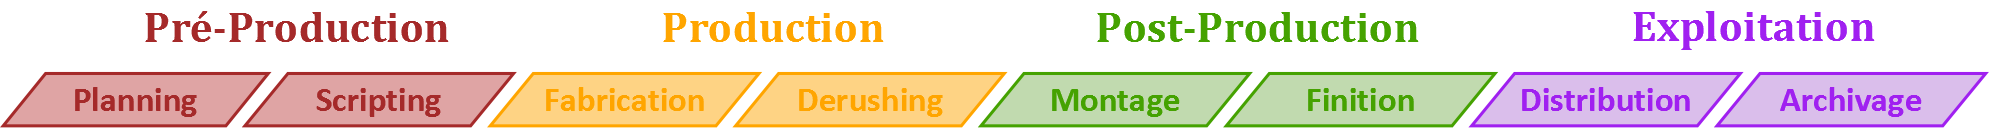
\includegraphics[width=\textwidth]{images/Workflow-Thesis-v0.png}
\caption{La chaîne de production audiovisuelle classique}
\label{img:intro:chaine}
\end{figure}


%%%%%%%%%%%%%%%%%%%%%%%%%
\subsubsection*{Préproduction}\label{sec:preprod}
L'objectif de cette étape est de construire une ébauche du futur document audiovisuel, de manière à prévoir les moyens à engager pour le réaliser. 
On distingue deux phases de préparation, l'écriture ou \e{Scripting} et le \e{Planning} ou planification.

À partir d'une idée, l'écriture du document se déroule en plusieurs étapes où l'on fixe progressivement le message à faire passer ainsi que sa forme audiovisuelle. 
Une fiction par exemple s'écrit à partir d'un résumé de l'histoire, puis on développe les scènes, les personnages, les lieux, les dialogues, etc. jusqu'à arriver à la manière dont cette histoire sera racontée à l'écran. 
On fixe ainsi le type de plan à filmer, les mouvements de caméra, le type de lumière, etc. 
Dans certaines grosses productions, on aura même recours au dessin pour aider à la représentation visuelle.


Toutes ces informations sur le contenu et la forme du futur document audiovisuel servent à estimer le temps nécessaire et les moyens à engager. 
L'estimation du coût d'une production est un élément essentiel pour la production audiovisuelle. 
En effet, dès le départ le producteur doit estimer la rentabilité du futur document afin de voir quels moyens il peut engager. 
Il s'agit bel et bien d'investissement, parfois très lourd, surtout en comparaison avec d'autres industries culturelles – musique, littérature, radio, presse – à l'exception récente du jeu vidéo. 
Contrainte budgétaire et forme esthétique sont donc en négociation dans cette première étape.


%%%%%%%%%%%%%%%%%%%%%%%%%
\subsubsection*{Production}
Une fois l'ébauche et les moyens déterminés, la production vise à réaliser chaque partie du document une à une puis à les assembler en un montage cohérent.

La phase de \e{Fabrication} consiste à capter du réel que l'on a mis en scène. La captation d'un évènement est réalisée grâce à des appareils d'enregistrement (caméra, microphones, etc.). 
La mise en scène du réel se construit à partir d'un ensemble de techniques, d'équipements et d'accessoires (lumière, costume, décors, maquillage, etc.) qui permettent d'obtenir l'image et le son souhaités. 
La technique est ainsi mobilisée dans un objectif esthétique. 
Dans le cas d'une fiction, la fabrication du contenu se fait en fonction du planning de mobilisation des personnes et des équipements plutôt que suivant l'ordre chronologique de l'histoire. 
On regroupe ainsi le tournage des scènes dans tel lieu ou avec tel équipement afin de réduire les coûts. Au final, la fabrication
produit des séquences vidéo et audio qu'il s'agit ensuite de redécouper pour mieux les assembler.

La phase de \e{Derushing} consiste à examiner les séquences réalisées pendant la fabrication et à les trier en vue de faciliter le montage. 
Par exemple, le tournage d'une fiction produit des séquences vidéo comprenant plusieurs prises d'une même scène et souvent des séquences captées par des caméras ayant des angles de prise de vue différents. 
Il faut donc redécouper les séquences en prises puis regrouper les prises d'une même scène. 
Le montage se fera d'autant plus facilement qu'on saura également identifier la qualité et les avantages de chaque prise d'une même scène.


%%%%%%%%%%%%%%%%%%%%%%%%%
\subsubsection*{Postproduction}
Lorsque le contenu audiovisuel est fabriqué et trié, il reste à le structurer en un document et à le conditionner en fonction de sa future exploitation.

La phase de \e{Montage} consiste à agencer des petites séquences de vidéo et d'audio pour construire la structure du document audiovisuel.
L'agencement des plans, leur durée et la transition entre ces plans constituent les ressorts esthétiques propres à l'audiovisuel. 
Ils participent à la transmission du message en ceci qu'ils servent de raccord entre les plans, comme le souligne le réalisateur \pc{Sergueï Mikhaïlovitch Eisenstein}\footnote{L'origine de cette fameuse citation est assez obscur, on la retrouve dans de nombreux documents, dont cet article --\cite{Montage et Réalisme}-- datant des années 60 et extrait de la revue québecoise \gui{Séquence : La revue du cinéma}.} :

\begin{cico}
Le montage est l 'art d'exprimer ou de signifier par le rapport de deux plans juxtaposés de telle sorte que cette juxtaposition fasse naître l'idée ou exprime quelque chose qui n'est contenu dans aucun des deux plans pris séparément. L'ensemble est supérieur à la somme des parties.
\end{cico}

Après le montage, une phase de \e{Finition} est nécessaire pour intégrer d'autres ressources au document en fonction de sa distribution. 
Pour une diffusion antenne d'un reportage, on ajoute le logo de la chaîne de télévision, un jingle, le nom des intervenants ou des titres, etc. 
Une diffusion sur DVD nécessitera l'ajout des conditions
légales d'usages, l'intégration d'un menu de navigation, etc. 
La distribution détermine également un format d'encapsulation (.avi, .mkv, .ogg etc.) et un encodage du contenu audiovisuel (MPEG-2, H.264, MPEG-4, theora vorbis etc.). 
Le résultat de cette phase de post-production est de fournir des documents prêts à l'usage et dans certains cas plusieurs variantes pour chacun des modes de distribution envisagés.


%%%%%%%%%%%%%%%%%%%%%%%%%
\subsubsection*{Exploitation}
Une fois le document achevé, on valorise sa construction par une distribution auprès d'une audience ainsi qu'un archivage qui permettra de le réutiliser ultérieurement.

La phase de \e{Distribution} consiste à rendre le document matériellement accessible à une audience. 
Il s'agit d'un transfert qui peut faire l'objet d'une transaction commerciale ou s'appuyer sur d'autres types de modèles économiques (publicité entre autres). 
La nature du transfert varie et porte à la fois sur les modalités d'accès au contenu et les droits d'usages.

La phase d'\e{Archivage} consiste le plus souvent à stocker le contenu diffusé afin de pouvoir le réutiliser tel quel plus tard, soit en le rediffusant, soit en le vendant à un autre diffuseur. 
C'est aussi généralement la phase où l'on construit, récupère et attache des descriptions du contenu au document audiovisuel. 
En effet, l'archivage n'a de sens que s'il permet de retrouver, voire redécouvrir, les documents archivés.
\ciel{Au plan économique, un film est un bien informationnel, d'expérience, caractérisé par une très forte densité d'informations. Son exploitation s'organise autour de versions différentes, distribuées sur des marchés distincts par des acteurs spécialisés.} (\cite{Blanc2006}).%Gilles Le Blanc - Innovations numériques, distribution et différenciation  : le cas de la projection numérique dans le cinéma.




%<TODO
%TODO>
\subsection{Documents et vocabulaire de la production}\label{sec:docvoc}
\e{
Dans cette section, nous présentons des définitions utilisées dans le milieu professionnel et tirées du \gui{Dictionnaire technique du Cinéma (\cite{Pinel2008})} afin de présenter les principaux documents et le vocabulaire utilisé pendant la phase de préproduction. 
Il s'agit ainsi de mettre en exergue la manière dont se construit une description textuelle de l'objet audiovisuel en devenir ainsi que le vocabulaire utilisé pour faire cette description.}
% Des éléments qui nous serviront à mieux cerner les problèmes qui se posent à la production audiovisuelle.

\paragraph{La notion de plan}
La notion de plan peut se présenter de diverses manières suivant le point de vue adopté. 
Du point de vue technique, il s'agit d'une série d'images (ou photogrammes) qui sont enregistré par un appareil de capatation (une caméra) au cours d'une même prise de vue : \ciel{série de photogrammes enregistrés au cours d'une même prise} (\cite{Pinel2008}).
Il s'agit donc de l'enregistrement qui est effectué entre le moment où l'on presse sur le bouton pour lancer et celui où l'on arrête l'enregistrement.
Cette définition, certes robuste, ne permet pas pour autant de caractériser les plans ou de les comparer entre eux. 
Ainsi, on s'intéresse au point de vue de l'écriture filmique et de la réalisation qui considère non seulement l'action d'enregistrement, mais également la manière dont il est effectué : 

\ciel{
Fragment de temps et d'espace enregistré d'un seul tenant, selon un point de vue déterminé, et donnant à la projection le sentiment de la continuité d'une même \e{image en mouvement}.} (\cite{Pinel2008})

Cette définition complète la précédente en considérant le rapport au sujet (le point de vue) et la temporalité du plan et son rapport à un ensemble d'autres plans (la continuité). 
Elle permet d'envisager les plans comme des éléments de base que l'on assemblera ensuite pour construire un objet audiovisuel : 

\ciel{
La notion de plan est apparue [\dots] lorsqu'on a abandonné le point de vue unique du tableau pour envisager le sujet sous différents angles et à différentes distances et lorsque, par la grâce du montage, on a mis en relation ces plans entre eux.
[\dots]
Si le photogramme représente l'unité technique de la prise de vues, la scène et la séquence les unités narratives de l'oeuvre cinématographique, le plan est la cellule fondamentale de l'écriture du film, de sa préparation jusqu'à la copie standard.} (\cite{Pinel2008})

Dans cette citation, on voit aussi émerger l'idée qu'il existe différents niveaux d'analyse dans l'objet audiovisuel : 
\begin{liste}
	\item un \g{niveau technique} avec le photogramme mais également le pixel dans le numérique.
	\item un \g{niveau narratif} avec la scène (unité de temps et de lieu dans l'histoire) et la séquence (suite de scènes constituant une action dramatique autonome ou distincte).
	\item \g{un niveau dont le plan est l'unité de base qui sert tout au long de la chaîne de production}. 
	On parle d'unité, car il s'agit du résultat de base d'une prise de vue, c'est-à-dire de la fabrication (production) de l'objet audiovisuel. 
	La pré-production, étape de préparation du tournage, utilise donc naturellement cette unité. 
	De même, le montage consiste à organiser ces plans pour former un ensemble cohérent, quitte à les ajuster (raccourcir, allonger, modification du cadrage etc.). 
	Ainsi, il semble que cette unité servent non seulement d'unité de travail de référence pour la chaîne de production\footnote{La production sonore d'un objet audiovisuel ne s'organise pas forcément de la même manière que celle de la production de l'image. Néanmoins, par la force des choses, la construction de l'image prime bien souvent sur celle du son et son unité de base sert donc de référence même pour la production sonore.}, mais également du premier niveau signifiant propre à l'audiovisuel (l'image seul pouvant être rattaché à la photographie).
\end{liste}

Ces distinctions nous permettent de définir le plan selon les caractéristiques suivantes : 
\begin{liste}
	\item \g{l'échelle relative du cadre par rapport au(x) sujet(s)} (personnages, objets etc.).
	C'est ce qui permet de définir un ensemble de \gui{valeurs de plan}, gros plan, plan américain etc. que nous définirons par la suite.
	
	\item \g{l'angle de la prise de vue} (plongée, contre-plongée, cadre incliné etc.)

	\item \g{le mouvement de la caméra} et d'autres paramètres de son objectif (panoramique, travelling, rotation, zoom, focale, focus etc.)

	\item \g{l'articulation des plans entre eux}, d'une part en terme de durée, mais aussi en terme de transition et d'impression de continuité entre les plans. 
	Par exemple, il existe des règles de cadrage et de montage pour aider les spectateurs à situer les personnes sur un plateau\footnote{La règle des 180° oblige ainsi à maintenir les mêmes relations est-à-gauche/droite-de entre les personnes, de manière à ce que le spectateur puisse se souvenir des positions des interlocuteurs sur un plateau. En inversant ces relations topographiques, on donne l'impression au spectateurs que les personnes ont échangé leurs places alors que c'est juste la caméra qui a changé de point de vue. Il s'agit donc d'une règle très importante pour assurer la continuité et la compréhension du spectateur.}.
\end{liste}


\paragraph{Valeurs de plan utilisées dans un script}
La valeur de plan est un des éléments le plus utilisé pour distinguer les plans entre eux, notamment au moment de l'écriture. 
Plutôt que de préciser les paramètres optiques de la caméra (considérés comme des détails très difficile à préciser à l'avance), le réalisateur préfère parler d'un type de plan pour donner une idée générale de l'image à obtenir. 
Le Tableau \ref{tab:vplans} présente les principales valeurs de plans utilisées par les professionnels, avec leur abréviations et leur(s) dénomination(s) anglaise(s) tandis que la Figure \ref{img:intro:plans} en propose une illustration.

\begin{table}[ht!]
   \begin{center}
		\begin{tabularx}{\textwidth}{|p{100pt}|X|p{100pt}|}
		   \hline
	\pc{Dénomination française} & \pc{Défintion} & \pc{Dénomination anglaise} \\ \hline\hline
 	\g{très gros plan (t.g.p.)} & plan cadrant une partie du visage, un détail du corps (un oeil, une bouche, un doigt etc.) ou le détail d'un objet. & extreme close-up, e.c.u. ; big close-up, b.c.u.\\ \hline

 	\g{gros plan (g.p.)} & plan isolant un visage, généralement cadré à la hauteur du noeud de cravate, ou un autre détail du corps (plan de détail ; insert), voire \e{tout ou partie d'un petit objet}. & close-up, c.u.\\ \hline

	\g{plan rapproché} & plan cadrant le(s) personnage(s) au niveau de la taille (plan rapproché taille, p.r.t.) ou de la poitrine (plan rapproché poitrine, p.r.p.). & medium close-up, m.c.u.\\ \hline
	
	\g{plan ceinture} & plan coupant les personnages au niveau de la ceinture & belt shot\\ \hline 

	\g{plan américain} (p.a.) & plan coupant les personnages à mi-cuisse & american shot ; medium close-shot, m.c.s.\\ \hline
	
	\g{plan moyen (p.m.) ou plan en pied} & plan présentant le(s) personnage(s) en pied. Il existe également des variations de ce plan qui sont nommées \e{serré} (aussi nommé plan américain large) ou \e{large} et qui font varier légèrement le cadrage. & medium shot, middle-shot, mid-shot, m.s. ; full shot, f.s.\\ \hline
	

	\g{plan de demi-ensemble (p.d.e., 1/2e.)} & plan mettant en place les personnages dans leur milieu en cadrant une bonne partie du décor & medium-long shot, m.l.s.\\ \hline

	\g{plan d'ensemble (p.e.)} & plan cadrant l'ensemble du décor construit & long shot, l.s.\\ \hline
	
	\g{plan de grand ensemble (p.g.e.)} & plan cadrant l'ensemble du décor construit de grande envergure. & very long shot, v.l.s.\\ \hline

	\g{plan général (p.g.)} & plan couvrant un vaste ensemble qui situe le décor construit dans son cadre : le décor dans le décor. & master shot ; extreme long shot, e.l.s\\ \hline 
		\end{tabularx}
		\caption{Valeurs de plans : du plus précis au plus général \label{tab:vplans}}
   \end{center}
\end{table}

% \begin{liste}
% 	\item \g{très gros plan} (t.g.p.) : \ciel{plan cadrant une partie du visage, un détail du corps (un oeil, une bouche, un doigt etc.) ou le détail d'un objet}. [extreme close-up, e.c.u. ; big close-up, b.c.u.]

% 	\item \g{gros plan} (g.p.) : \ciel{plan isolant un visage, généralement cadré à la hauteur du noeud de cravate, ou un autre détail du corps} (plan de détail ; insert), voire \ciel{tout ou partie d'un petit objet}. [close-up, c.u.]

% 	\item \g{plan rapproché} : \ciel{plan cadrant le(s) personnage(s) au niveau de la taille (plan rapproché taille, p.r.t.) ou de la poitrine (plan rapproché poitrine, p.r.p.).} [medium close-up, m.c.u.]
	
% 	\item \g{plan ceinture} : plan coupant les personnages au niveau de la ceinture [belt shot] 

% 	\item \g{plan américain} (p.a.) : \ciel{plan coupant les personnages à mi-cuisse} [american shot ; medium close-shot, m.c.s.]
	
% 	\item \g{plan moyen} (p.m.) ou \g{plan en pied} : \ciel{plan présentant le(s) personnage(s) en pied.} [medium shot, middle-shot, mid-shot, m.s. ; full shot, f.s.]
% 	Il existe également des variations de ce plan qui sont nommées \ciel{serré} (aussi nommé plan américain large) ou \ciel{large} et qui font varier légèrement le cadrage.

% 	\item \g{plan de demi-ensemble} (p.d.e., 1/2e.): \ciel{plan mettant en place les personnages dans leur milieu en cadrant une bonne partie du décor}. [medium-long shot, m.l.s.]

% 	\item \g{plan d'ensemble} (p.e.) : \ciel{plan cadrant l'ensemble du décor construit}. [long shot, l.s.]
	
% 	\item \g{plan de grand ensemble} (p.g.e.) : \ciel{plan cadrant l'ensemble du décor construit de grande envergure}. [very long shot, v.l.s.]

% 	\item \g{plan général} (p.g.) : \ciel{plan couvrant un vaste ensemble qui situe le décor construit dans son cadre : le décor dans le décor}. [master shot ; extreme long shot, e.l.s] 
% \end{liste}
%TODO:source

\begin{figure}[ht!]
\centering
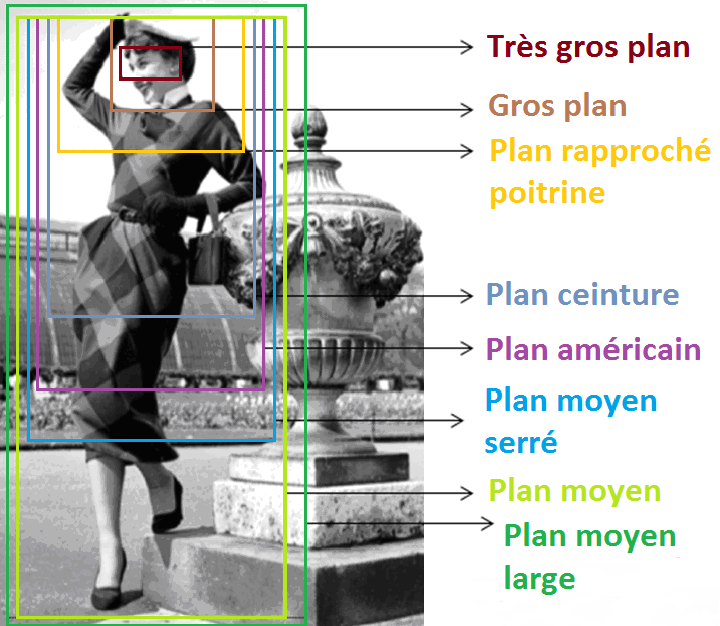
\includegraphics[width=0.4\textwidth]{./images/ValeurPlan-v1.png}
\caption{Différentes valeurs de plan pour le cadrage d'un personnage à l'écran}
\label{img:intro:plans}
\end{figure}


\paragraph{Quelques documents de (pré)production}
%TODO:description + source
La pré-production se repose sur différents types de documents qui permettent de faire émerger progressivement la structure narrative ou documentaire, le découpage en plans et tous les détails de réalisation nécessaire à une bonne préparation du tournage. 
On notera que chacun de ces documents constitue un jalon dans la préparation du projet et que le script, résultat final de cette écriture, constitue une sorte de cahier des charges de l'objet audiovisuel à fabriquer.
\begin{liste}
	\item \g{sujet} : \ciel{matière première du film enrichie et développée lors de la préparation puis mise en forme au cours de la réalisation et du montage.} 
	
	\item \g{synopsis} : \ciel{exposé sommaire en quelques lignes, voire en quelques pages, du contenu dramatique ou documentaire d'un film}. 
	À noter que ce document est également utilisé plus tard dans la chaîne de production, notamment pour être transmis aux journalistes ou aux archivistes.
	De plus, il constitue la première mise en forme narrative du contenu du film, à la différence du sujet qui ne se constitue que de quelques idées directrices. 

	\item en cas d'adaptation d'une oeuvre littéraire en un objet audiovisuel, on développe un \g{traitement} : 
	\ciel{Travail littéraire préparatoire effectué à partir d'une oeuvre pré-existante ou d'une oeuvre originale pour assurer sa transmutation en termes cinématographiques.}

	\item lorsqu'on développe un objet audiovisuel original, à défaut de traitement on peut parler de \g{scénario} :
	\ciel{description de l'action d'un film épousant la forme \e{littéraire} du récit, rendant compte des articulations narratives et comportant une ébauche des dialogues, quelquefois la description plus précise de certaines scènes-clefs.}

	\item lorsque le besoin de préciser encore la construction de la narration, les auteurs peuvent construire une \g{continuité (dialoguée)} : \ciel{étape de la préparation écrite du film qui permet d'enrichir le traitement en développant chronologiquement les fragments d'action, en mettant au point le détail de chaque scène et en précisant le dialogue.}

	\item \g{plan de tournage} : \ciel{ultime travail de préparation effectué par le réalisateur avant le tournage. Il consiste à fragmenter la continuité en unités cinématographiques de temps et d'espace : les plans.}

	\item \g{script} : \ciel{dernière mouture du scénario, guide complet du tournage}.La Figure \ref{img:intro:script} présente un exemple de script extrait d'un film récent écrit et réalisé par Quentin Tarantino.
\end{liste}

\begin{figure}[ht!]
\centering
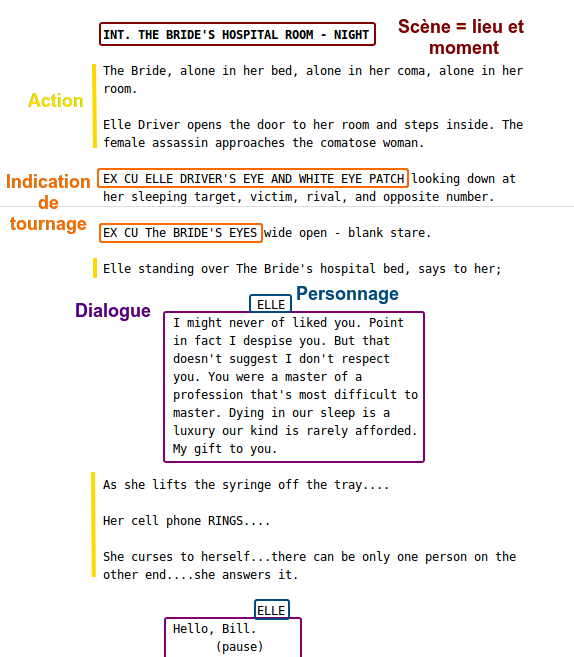
\includegraphics[width=0.7\textwidth]{images/ScriptExample-v1.png}
\caption{Extrait du script de Kill Bill écrit et réalisé par Quentin Tarantino}
\label{img:intro:script} 
\end{figure}

% des réécritures de documents et des mises à jours qui pourraient être réalisées par des machines, des informations qui pourraient être transmises automatiquement à travers un réseau numérique d'information


% un vocabulaire bien défini qui fait l'objet de nombreux dictionnaires, donc prêt à être formalisé


% des équipes qui sont réduites lors de tournage en extérieur




%%%%%%%%%%%%%%%%%%%%%%%%%%%%%%%%%%%%%%%%%%%%%%%%%%%%%%%%%%%%%%%%%%%%%%%%%%%%%%%%%%%%%%%%%%%%%%%%%%%
\subsection{Besoins Métiers}\label{sec:besoins}
\e{
Face à une numérisation qui fragmente les contenus, une mise en réseau qui facilite la fabrication amateur, intensifie la circulation de ces fragments (\ref{sec:motiv}), la production audiovisuelle rencontre de nouveaux défis qui remettent en jeu son organisation et sa manière de se représenter le monde. 
Ainsi d'une part la fragmentation ne doit pas mettre en péril la cohérence de l'ensemble et d'autre part, la circulation des contenus ne doit pas compromettre l'exploitation future du tout ou des parties. 
L'ouverture d'une chaîne de production à des acteurs tiers implique de clarifier les attendus de chacun. 
Lorsqu'il s'agit de faire fabriquer ou de récupérer du contenu, il devient nécessaire pour le client de décrire la commande de contenu au fournisseur, de même que le fournisseur doit décrire à son client le contenu livré pour faciliter son exploitation. 
Ainsi, on souhaite adjoindre aux contenus des descriptions qui permettent de faciliter leur recherche et leur manipulation.
}


Pour les professionnels de la production audiovisuelle, le défi porte à la fois sur l'organisation de leur chaîne de production et sur la gestion de leurs produits :
\begin{liste}
	\item[(1)] \g{comment transformer la chaîne de production afin de l'ajuster à la diversification des formes de fabrication et de distribution des contenus, mais aussi aux changements dans les pratiques de consommation des audiences ?}

	\item[(2)] \g{comment passer d'une gestion de fichiers à une gestion de contenus audiovisuels considérés comme des objets numériques fragmentés dont il s'agit de garantir l'autonomie dès leur conception et jusque dans leurs différents cadres d'exploitation ?}
\end{liste}

% Problèmes métiers ? Tant que ça ne devient pas une solution, mais des tendances à prendre en compte 

On peut ensuite détailler ces défis en objectifs plus précis :
\begin{liste}
	\item[(1a)] \e{accorder contribution amateur et production professionnelle pour fabriquer ou valoriser du contenu.}

	L'amélioration croissante des capteurs des appareils multimédia ajoutée aux capacités de communication offrent au grand public de plus en plus de manières de participer aux processus de fabrication ou de diffusion des contenus.
	Les possibilités accrues de participation au processus médiatique (participation à l'émission, envoi de contenu, propagation via ses contacts, commentaires etc.) valorisent le spectateur, le contenu et la plate-forme de diffusion (comme d'une certaine manière peut le faire le bouche à oreille).

	De manière générale, l'intégration de contenus externes dans une chaîne de production professionnelle ne s'envisage  qu'à partir d'un certain niveau de qualité du contenu livré.  
	Paradoxalement, dans certains cas les signes d'une production amateur (tremblements, caméra à l'épaule etc.) peuvent être revendiquées comme des marque de style qui suggère une collaboration avec le public ou une proximité avec une réalité éloignée des images diffusées par les médias.
	Ainsi, les professionnels souhaitent encadrer plus ou moins fortement la production amateur par des indications, recommendations, obligations.\\


	\item[(1b)] \e{créer de nouvelles étapes dans la chaîne visant à réutiliser les contenus existants et les adapater à de nouveaux modes de consommation.}

	L'augmentation de l'offre de contenus accessibles aux spectateurs (chaînes, enregistrements, balladodiffusion, vidéo à la demande etc.) se traduit par une mise en concurrence accrue des contenus diffusés par les professionnels.
	Le contrôle de l'offre n'étant plus atteignable, il faut adopter de nouvelles stratégies de valorisation des contenus produits ou diffusés pour maintenir leur visibilité et leur rentabilité. 
	Une autre approche consiste à fournir un service de recommandation aux spectateurs et ainsi rentrer dans une démarche de fidélisation. 

	Par ailleurs, l'augmentation des terminaux de lecture multimédia et leur portabilité offrent de plus en plus d'occasions aux spectateurs de consommer des contenus. 
	Par exemple, les situations de mobilités peuvent impliquer des capacités de transfert diminués, un écran plus petit, des temps de disponibilités plus courts etc.
	Il semble alors que la production doivent évoluer pour fournir de nouveaux formats ou des formes retravaillées de contenus existants.

	Dans tous les cas, cela implique de se consacrer à des tâches d'éditorialisation des contenus pour répondre aux exigences et aux attentes de ces nouveaux modes de consommation.\\
% \end{liste}


% \begin{liste}
	\item[(2a)] \e{gérer l'intégration de contenu externes, les variations d'un même contenu pour les rattacher à un même objet numérique.} 
	% représentation

	L'utilisation de contenus provenant de sources externes de même que la production de multiples variations d'un même contenu augmente le nombre de ressources à gérer. 
	De plus, les relations entre ces différentes ressources nécessitent d'être clarifiées et explicitées dans le système de gestion. 
	% chaîne éditoriale ? 
	
	Il ne s'agit plus simplement de gérer des fichiers mais un ensemble de fichiers et de données qui constituent un ensemble cohérent et fragmenté que l'on nomme un objet numérique. 
	Cet objet doit intégrer à la fois les diverses sources qui le composent mais aussi des variations correspondants aux exploitations visées, des descriptions et tout ce qui permet de garantir son autonomie. 
	Il doit également s'agir d'un objet \e{métier} car son statut, son organisation, sa sémantique correspondent à la vision d'un métier, à la manière dont il pense le monde. 

	% Ainsi, on ne souhaite plus gérer des fichiers mais des objets numériques qui doivent acquérir un statut, une sémantique correspondant à la manière dont les métiers de la production les considèrent.\\
	% qui possède une valeur et une sémantique propre à un contexte d'usage. 	


	\item[(2b)] \e{associer des descriptions aux contenus pour faciliter leur exploitation dans un environnement numérique.}
	% description

	L'augmentation des contenus audiovisuels en circulation, la diversification de leurs modes d'exploitation compliquent la gestion des contenus.  
	Afin de favoriser la réutilisation de ces contenus, il faut pouvoir leur attacher des informations pertinentes pour les professionnels qui les manipulent. 
	La description du contenu peut varier suivant les besoins de chaque métier impliqué dans la chaîne de production. 
	Les opérations n'étant pas les mêmes, les descriptions de ces opérations varient donc également et sont nécessaires pour faciliter la réutilisation du contenu. 
	%de manière à faciliter modalités d'exploitation envisagées  

	Lorsque la réutilisation et production s'entremêlent, il est également nécessaire de construire les descriptions en même temps que le contenu. 
	De cette manière on récupère ou on réévalue l'information à mesure de l'avancée dans la chaîne. 

	Cela nécessite d'informatiser l'étape de pré-production de la chaîne et de modéliser les informations utilisées par les professionnels. 
	%commencer plus tôt, avoir plusieurs niveaux/types de description, raccrocher les bons éléments à la représentation de l'objet numérique
	
	%et embarquent des descriptions explicitant leurs modalités d'exploitation.

\end{liste}

\e{
En guise de synthèse, nous pouvons dire qu'il s'agit de constituer des objets audiovisuels autonomes dans les chaînes de production audiovisuelle. 
Nous précisons ce caractère autonome, car ces objets seront porteurs de leur propre description et associés à des connaissances sur l'organisation de la chaîne de production dans lesquels ils évoluent.
Ainsi, ces objets audiovisuels pourront être (ré)introduits à n'importe quelle étape d'une chaîne de production et fourniront aux contributeurs concernés des informations propres à faciliter leur (ré)utilisation.
}
	% \item \eg{valoriser et éditorialiser les contenus existants pour les rendres plus visibles, plus attrayants auprès des audiences ciblées.}
	% L'augmentation de l'offre de contenus accessibles aux spectateurs (chaînes, enregistrements, balladodiffusion, vidéo à la demande etc.) se traduit par une mise en concurrence accrue des contenus diffusés par les professionnels.

	% Le contrôle de l'offre n'étant plus atteignable, il faut adopter de nouvelles stratégies de valorisation des contenus produits ou diffusés pour maintenir leur visibilité et leur rentabilité. 
	% Une autre approche consiste à fournir un service de recommandation aux spectateurs et ainsi rentrer dans une démarche de fidélisation. 
	% Cela implique de se consacrer à des tâches d'éditorialisation des contenus pour des audiences plus ciblées.
	
	% \item \eg{produire de nouvelles formes de contenus ou adapter les rmes existantes pour satisfaires aux nouveaux modes de distribution/consommation.}
	% L'augmentation des terminaux de lecture multimédia et leur portabilité offrent de plus en plus d'occasions aux spectateurs de consommer des contenus. Par exemple, les situations de mobilités peuvent impliquer des capacités de transfert diminués, un écran plus petit, des temps de disponibilités plus courts etc.
	% Il semble alors s'ouvrir une place pour de nouveaux formats ou des formes retravaillés de contenus existants. 
	% Il s'agit de faire de la production multi-support et d'adapter les contenus en fonction des conditions de distribution et de l'audience visé (réutilisation).
	
	% \item \eg{articuler la contribution amateur avec la chaîne de production professionnelle.}
	% L'amélioration croissante des capteurs des appareils multimédia ajoutée aux capacités de communication offrent au grand public de plus en plus de manières de participer aux processus de fabrication ou de diffusion des contenus.
	% Les possibilités accrues de participation au processus médiatique (participation à l'émission, envoi de contenu, propagation via ses contacts, commentaires etc.) valorisent le spectateur, le contenu et la plate-forme de diffusion.

	% Cependant, il faut être capable d'intégrer ces contributions externes au sein de la production professionnelle en les encadrant plus ou moins fortement, par des indications, recommendations ou des contraintes.

	% \item \eg{gérer les objets audiovisuels dès le début et tout au long de leur cycle de vie.}
	% %
	
	% Une circulation plus importante des contenus implique de trouver un moyen de gérer non plus des fichiers mais des objets numériques qui unifient plusieurs variations d'un même contenu et embarquent des descriptions explicitant leurs modalités d'exploitation.



% numériser => (a) fragmenter + (b) mettre en réseau => (a) besoin de conserver la cohérence de l'ensemble + (b) besoin d'autonomiser pour une future situation d'usage








%%%%%%%%%%%%%%%%%%%%%%%%%%%%%%%%%%%%%%%%%%%%%%%%%%%%%%%%%%%%%%%%%%%%%%%%%%%%%%%%%%%%%%%%%%%%%%%%%%%
% \newpage
\section{Problèmes}\label{sec:prob}



%%%%%%%%%%%%%%%%%%%%%%%%%%%%%%%%%%%%%%%%%%%%%%%%%%%%%%%%%%%%%%%%%%%%%%%%%%%%%%%%%%%%%%%%%%%%%%%%%%%
\subsection{Problèmes métiers}\label{sec:pmetiers}
% Nos champs d'applications sont : 
% Prenant acte des besoins de la production audiovisuelle nous distinguons deux problèmes métiers (1) identifier le(s) niveau(x) de fragmentation et (2) le(s) type(s) de description susceptibles de favoriser la fabrication mixte, la circulation et la réutilisation des contenus.
% Ces problèmes remettent en cause à la fois la représentation classique des contenus et leur description. 
% de manière à faciliter (1) la production mixte amateur-professionnel et (2) leur réutilisation dans de nouveaux contextes d'exploitation.
% l'informatisation du début de la chaîne de production, préproduction 
% l'inscription formelle de l'écriture audiovisuelle ?

\e{
L'objectif central qui se pose à la production audiovisuelle est de constituer des objets audiovisuels autonomes et donc (ré)utilisable à n'importe quel étape de la chaîne. 
Or, dans la chaîne de production classique les programmes n'émergent qu'à la fin de la chaîne et sont gérés d'une pièce. 
Il n'y a pas forcément de place pour les éléments de contenu intermédiaires, et c'est justement à la modélisation de ces fragments que l'on s'attaque. 
Ces fragments doivent devenir des éléments documentaires qui possèdent leur unité propre de même que les objets finis que sont les programmes. 
Une des difficultés réside dans cette articulation entre des fragments et le tout ou l'ensemble que constitue les programmes. 
Par ailleurs, il existe des problèmes sous-jacents à cette fragmentation documentaire : 
}
\begin{liste}
	\item \e{identifier quels niveaux de fragments peuvent prétendre à ce genre de transformation}.
	Si le numérique permet de fragmenter à l'envie, il faut cependant prendre en compte les pratiques du métier pour identifier les niveaux de fragmentation pertinents ou déjà utilisés dans le métier mais non modélisés.
	Par exemple, la prise de vue est le résultat d'une activité de tournage, pour autant elle ne constitue pas un objet éditorial comme peut l'être une interview.
	De plus, il s'agit également de déterminer comment manipuler ces fragments comme des objets à part entière sans compromettre l'articulation de l'ensemble. 
	Par exemple, une interview peut s'intégrer dans un journal télévisé ou bien un reportage dans des versions plus ou moins courtes. 
	Pour autant, il s'agit du fruit d'une même activité, simplement le montage, et donc le résultat, est différent suivant le programme dans lequel l'interview s'insère.\\
	
	\item \e{identifier quelles informations et connaissances doivent être rattachées à ces fragments pour les rendre autonome}.
	D'une manière similaire à la démarche pour les objets entiers, certaines connaissances, notamment relatives au contexte de production, doivent être attachées au fragment pour garantir sa réutilisation et sa cohérence. 
	En reprenant l'exemple de la prise de vue, on peut lui associer le bout de script qui a prescrit ce qu'elle devait montrer. 
	Si l'on pousse encore cette logique, il faut également incorporer le document qui définit le programme pour lequel on a tourné cette prise de vue, la personne qui l'a effectuée, les équipements utilisés etc. 
	Ainsi, on étend la modélisation de l'objet audiovisuel à son contexte de production et tout ce qui renforce les possibilités de recherche, de manipulation, de gestion et de transformation de ces objets. 
	De plus, s'ajoute à cela la question de la collecte de ces informations. 
	En effet, la saisie de ces informations au sein d'un système d'information et leur utilisation par les acteurs de la chaîne n'est pas une simple formalité.
	Ce problème pousse également dans le sens d'une modélisation plus contextuelle, de manière à proposer un environnement de travail adapté et utilisable aux contributeurs de la chaîne.\\
	
	% \item \e{}.
\end{liste}


% Notre problème se situe dans le croisement de la représentation des contenus et la représentation des activités humaines qui construisent, manipulent, éditent, transforment, publient et documentent ces contenus. 
% Cet angle de recherche nous amène donc à considérer non pas le contenu audiovisuel dans son ensemble, une fois terminé et validé, mais la construction de tout ces fragments qui le composent. 
% Il nous faut aussi considérer, non pas seulement le contenu audiovisuel, mais aussi d'autres informations, d'autres documents qui constituent son contexte de production, dans un sens très général. 
% Chaque prise de vue constitue donc un objet à représenter en tant que tel, tout autant que le bout de script qui a prescrit ce que cette prise de vue devait montrer. 
% Si l'on pousse encore cette logique, on peut alors représenter de même le document qui définit le programme pour lequel on a tourné cette prise de vue, la personne qui l'a effectué, les équipements utilisés etc. 
% Ainsi, on étend la représentation du contenu à son contexte de production entendu comme toutes les informations qui renforceront les possibilités de recherche, de manipulation, de gestion et de transformation de ces contenus. 

%%%%%%%%%%%%%%%%%%%%%%%%%%%%%%%%%%%%%%%%%%%%%%%
\subsection{Problèmes scientifiques}\label{sec:scien}
Au fur et à mesure que la circulation des contenus s'intensifie, il y a un besoin grandissant de faciliter l'échange d'information tant à la fois sur le plan informatique, que sur le plan humain. 
De plus, l'ouverture de la chaîne de production à de nouveaux contributeurs (amateurs et professionnels) ne fait qu'accentuer la disparité des connaissances et des systèmes utilisés. 
Afin de construire une compréhension commune à tous les contributeurs au cycle de vie, on fabrique un modèle conceptuel capable d'intégrer et de mettre en relation leurs connaissances. 
Il s'agit là d'un apport par rapport à la situation existante où le consensus n'existait pas, ou alors de manière éphémère, locale au sein d'une équipe.
L'objectif est de fluidifier les échanges d'information et de contenus en formalisant les connaissances utilisées pour :
\begin{problemes}{LightGoldenrodYellow}
\begin{liste}
% modéliser tous les objets de la chaîne de production audiovisuelle
	\item[(A)] \g{modéliser les objets construits au fil de la chaîne de production audiovisuelle}.
	\item[(B)] \g{modéliser les connaissances sur ces objets} (descriptions, contexte de production, contribution au cycle de vie).
	% \item[(B)] décrire les objets audiovisuels
	% \item[(C)] représenter la contribution de chacun des acteurs au cycle de vie des objets audiovisuels
\end{liste}
\end{problemes}

\e{
Ainsi, notre problème de recherche général s'articule autour de la modélisation des connaissances et des informations que les contributeurs construisent, utilisent, échangent au cours du cycle de vie des objets audiovisuels. 
Cette modélisation constitue une première étape dans la mise en place d'un système d'information servant à mieux gérer les objets audiovisuels et médier la communication entre systèmes informatiques tout autant qu'entre contributeurs humains.
Après avoir numérisé les contenus audiovisuels, on souhaite transformer chaque élément les composant en objet documentaire et documenter leur cycle de vie.\\}



\g{(A)} Le problème est d'organiser la gestion des objets audiovisuels en proposant une modélisation capable de faciliter leur identification, leur manipulation et leur réutilisation tout au long de leur cycle de vie. 
En particulier,	l'objet audiovisuel professionnel est produit de manière collective, chaque contributeur apportant un élément à l'ensemble. 
Ces contributions doivent donc pouvoir être identifiées comme appartenant à un ensemble, de même que chaque élément doit pouvoir être considéré pour soi afin d'être intégré dans un autre ensemble (réutilisation).

Pour cela on adopte une représentation des différents niveaux d'abstraction des objets audiovisuels numériques de façon à rétablir les liens entre les différentes versions ou copies d'un même contenu, quelque soit la nature des variations entre elles (encodage, format d'encapsulation, montage, finition, langue etc.).
La distinction entre différents niveaux de modélisation (technique, esthétique, éditorial etc.) doit permettre de construire une représentation dynamique de l'objet audiovisuel qui suit l'avancement du processus de production.\\
% La distinction entre différents niveaux de modélisation (technique, esthétique, éditorial etc.) doit permettre de construire une représentation de l'objet audiovisuel au fur et à mesure de l'avancement du processus de production.\\


\g{(B)} Le problème est d'attacher plusieurs types de connaissances aux objets audiovisuels de manière à les rendre autonomes dans leur circulation et leur réutilisation. 
Afin de faciliter l'échange d'information et la réutilisation des objets audiovisuels entre différents contextes, il faut modéliser des connaissances sur ces objets qui sont parfois déjà existantes mais non formalisées, ou bien qu'il faut rendre compréhensibles.
En effet, l'échange d'informations dans la production audiovisuelle est primordial et s'effectue entre métiers ou organisations différent(e)s, voire avec des amateurs. 
En particulier, on souhaite s'appuyer sur le vocabulaire de l'écriture filmique utilisé dans des documents de préproduction pour spécifier les résultats attendus de la production.
L'information contenue dans ces documents est importante mais repose sur des conventions plus ou moins tacites qu'il faut expliciter pour les professionnels, expliquer pour les amateurs.
La formalisation de ces éléments devra donc pouvoir être lu et modifié tout au long du cycle de vie des objets audiovisuels par tout types de contributeurs.

% échange d'info, adaptation par l'explicitation du vocabulaire et la contribution au cycle de vie
La formalisation de l'écriture filmique permettra d'adapter la présentation de l'information en fonction des connaissances, de l'implication du contributeur dans la chaîne (rôle, tâche, niveau de compétences etc.), de son référentiel professionnel ou linguistique. 
Il s'agit alors d'établir des correspondances entre les connaissances connues par le lecteur d'une information et celles utilisées par la personne qui l'a exprimée.
Ainsi, d'une part on explicite l'expression de l'information, ce qui permet l'adpatation, et facilite son interprétation ultérieure.
Le processus prend tout son sens lorsqu'il s'agit de traduire un concept de la réalisation audiovisuelle pour guider un amateur dans son tournage.
% Par exemple, l'action écrite par l'auteur et transformé en scène par le réalisateur, doit ensuite être tourné un caméraman, des acteurs etc. 


% réutilisation, attachement des connaissances pertinentes pour manipuler ou exploiter chaque fragment ou l'objet en entier
De plus, les descriptions utilisées, en plus de permettre de spécifier le résultat attendu de la production, doivent permettre de faciliter la recherche, la manipulation et la réutilisation des objets audiovisuels.
Pour cela, il faut articuler ces connaissances aux objets et aux fragments qui les composent. 
Le vocabulaire de l'écriture filmique sera également précieux, puisqu'il nous donne une unité de base, le plan, ainsi que ses caractéristiques qui permettent de le distinguer des autres. 
La recherche dans des dépôts de contenus se fera ainsi de manière similaire à la commande de contenu à d'autres contributeurs, qu'ils soient professionnels ou amateurs.



% Il s'agit donc de définir un modèle de description susceptible d'être utilisé par les contributeurs professionnels ou amateurs, à toutes les étapes de la chaîne de production. 


% Afin de décrire les contenus, on souhaite s'appuyer sur le vocabulaire de l'écriture audiovisuelle utilisé dans les différentes étapes de la chaîne et notamment dès la préproduction. 
% Cette écriture repose sur un vocabulaire des techniques de réalisation audiovisuelle (prise de vue, transition, composition de l'image etc.) renvoyant à des effets largement connus dans le milieu de l'audiovisuel et chez les cinéphiles. 
% L'écriture est utilisée avant la fabrication du contenu pour la spécifier, puis pendant la fabrication pour enregistrer les différences. 
% Une formalisation de ce vocabulaire permettrait de construire une description textuelle d'un contenu à partir d'une description objective de la réalisation (réglages des appareils, position des acteurs etc.).\\



% \g{(C)} Le problème est de représenter et faciliter l'échange d'information entre des contributeurs hétérogènes dans leurs connaissances et leur implication dans la chaîne de production.
% Une première diffculté réside dans l'articulation entre les connaissances des contributeurs qui expriment l'information et ceux qui l'interprèteront.
% La seconde diffculté consiste dans l'articulation des représentations du cycle de vie, de l'objet audiovisuel et des descriptions qui leurs sont associées. 
% En effet, chaque contributeur peut participer à la constitution d'informations associées au contenu en cours de sa production.
% Ces informations varient en fonction de l'implication du contributeur dans la chaîne (rôle, tâche, niveau de compétences etc.). 
% De plus, les informations construites à un moment sont susceptibles d'être utilisées plus tard dans la chaîne, par un contributeur ne partageant pas forcément les mêmes connaissances ou le même référentiel professionnel ou linguistique.

% On cherche alors à réaliser une adaptation de la forme d'expression de ces informations afin de faciliter le déroulement du processus de production. 
% Dans un premier temps, on explicite les connaissances utilisées par un premier utilisateur pour exprimer une information. 
% Ensuite, on établit une correspondance avec les connaissances connues d'un autre utilisateur et on adapte au besoin la forme de d'expression de cette information pour faciliter son interprétation. 
% L'adpatation qui en résulte prend tout son sens lorsqu'il s'agit de traduire un concept de la réalisation audiovisuelle pour guider un amateur dans son tournage.


%%%%%%%%%%%%%%%%%%%%%%%%%%%%%%%%%%%%%%%%%%%%%%%
% \section{Positionnement Disciplinaire (n,i)}\label{sec:posd}
% [Ingénierie des connaissances ; Media Asset Management ; Gestion électronique de Documents ; Ingénierie documentaire]
% ingénierie des connaissances (représentation des connaissances) ingénierie des inscriptions numériques de connaissances, dont les documents
% ingénierie documentaire (modélisation des documents propres à la production audiovisuelle)
% indexation et gestion des connaissances (description des contenus audiovisuels)
% la ged s'occupe de la gestion de documents, nous proposons de gérer des fragments de documents, de gérer leur construction en plusieurs étapes, par plusieurs acteurs et dans le cadre de différentes missions.

% Pour définir cet ensemble d'informations qui forment le contexte de production, nous nous sommes appuyés sur les partenaires du projet MediaMap. 



% des réécritures de documents et des mises à jours qui pourraient être réalisées par des machines, des informations qui pourraient être transmises automatiquement à travers un réseau numérique d'information
% un vocabulaire bien défini qui fait l'objet de nombreux dictionnaires, donc prêt à être formalisé
% des équipes qui sont réduites lors de tournage en extérieur

% à mettre dans le pos. disciplinaire, comment on aborde les problèmes posées
% [Nous avons ainsi dégagé plusieurs perspectives métiers qui nous ont servi de guide pour identifier les échanges d'informations les plus importants ainsi que le vocabulaire utilisé pour les exprimer. 
% Chacune de ces perspective possède un objectif propre et des spécificités, cependant il apparaît qu'un langage commun est utilisé par tous les acteurs de la production. 
% En se concentrant sur la description d'un contenu existant ou à venir, ce langage permet à ces acteurs de communiquer entre eux. Le réalisateur qui spécifie un attendu dans son script, les caméraman qui réalisent le cadrage, les opérateurs lumières etc. 
% Tous utilisent ce langage pour imaginer le résultat à produire et en déduire les gestes à opérer. 
% Les usages n'étant jamais complètement figé, chaque organisation développe ses propres idiomatismes de langage. 
% Dans ce cas, la collaboration entre organisations impliquent de pouvoir réaliser des ajustements dans l'expression de la description du contenu. 
% De même, la collaboration avec des contributeurs amateurs soulève un problème de compréhension de ce langage (et donc de l'attendu) mais aussi de connaissances des gestes à opérer (pour produire le résultat attendu).
% Ainsi, à mesure que la circulation des contenus s'intensifie, que les besoins de collaboration augmentent, naît un besoin grandissant d'explicitation des échanges d'information afin de dégager une vue d'ensemble de la chaîne de production, de ses acteurs, de leurs interactions, de leurs produits. 

% Notre proposition consiste à modéliser ces éléments et à en informatiser l'accès de manière à fluidifier les échanges de contenus et faciliter la compréhension des informations afférentes.] 


% \cleardoublepage





%%%%%%%%%%%%%%%%%%%%%%%%%%%%%%%%%%%%%%%%%%%%%%%%%%%%%%%%%%%%%%%%%%%%%%%%%%%%%%%%%%%%%%%%%%%%%%%%%%%
%%%%%%%%%%%%%%%%%%%%%%%%%%%%%%%%%%%%%%%%%%%%%%%%%%%%%%%%%%%%%%%%%%%%%%%%%%%%%%%%%%%%%%%%%%%%%%%%%%%
\part*{État de l'Art}
%%%%%%%%%%%%%%%%%%%%%%%%%%%%%%%%%%%%%%%%%%%%%%%%%%%%%%%%%%%%%%%%%%%%%%%%%%%%%%%%%%%%%%%%%%%%%%%%%%%
%%%%%%%%%%%%%%%%%%%%%%%%%%%%%%%%%%%%%%%%%%%%%%%%%%%%%%%%%%%%%%%%%%%%
%%%%%%%%%%%%%%%%%%%%%%%%%%%%%%%%%%%%%%%%%%%%%%%%%%%%%%%%%%%%%%%%%%%%
%%%%%%%%%%%%%%%%%%%%%%%%%%%%%%%%%%%%%%%%%%%%%%%%%%%%%%%%%%%%%%%%%%%%
%%%%%%%%%%%%%%%%%%%%%%%%%%%%%%%%%%%%%%%%%%%%%%%%%%%%%%%%%%%%%%%%%%%%
\chapter{Outils de modélisation}\label{c:omod}


% pourquoi on parle de SOC ? Parce qu'on souhaite représenter des objets audiovisuels, leur production, leur description et que ceci ne peut se faire sans une représentation du vocabulaire utilisé dans la production audiovisuelle. 

Dans le cadre de la production audiovisuelle collaborative, qui implique à la fois des amateurs et des professionnels, un des enjeux que nous avons noté (\ref{sec:scien}) est de rendre plus compréhensible l'échange d'informations entre contributeurs. 
D'une part, nous avons des practiciens professionnels utilisant un ou plusieurs vocabulaires métiers suffisamment définis pour que l'on puisse en faire des dictionnaires (\cite{Journot2008}; \cite{Pinel2008}). 
Ces personnes font usage de la langue d'une manière précise, régie par des conventions et portée par une conception de la production audiovisuelle et de ses objets, que l'on suppose stabilisée, au moins localement (au sein d'un même pays, d'une même école de pensée, organisation, équipe etc.).
Toutefois, on s'attend à des variations dans les usages de la langue, au même titre que l'on suppose qu'il existe des variations entre pratiques des gens du métiers.
Cependant, il semble qu'il s'agit seulement de variations et qu'il soit possible alors d'identifier les éléments communs et distincts.

D'autre part, les amateurs, quant à eux, n'ont pas le support de ces conventions travaillées au quotidien.
Ils sont, au mieux, des intermittents éclairés qui ont saisi le sens d'éléments de langage propres aux métiers (par des lectures, des rencontres, des formations etc.). 
Il faut donc supposer qu'il y a tout à expliquer à ces amateurs, plutôt que de parier sur leur compréhension innée des métiers de la production audiovisuelle.
En particulier s'il s'agit de demander du contenu à des amateurs sous la forme d'un script de tournage, il faudra alors trouver un moyen d'expliciter cette commande et d'expliquer ou d'assister sa réalisation. 

Ainsi, l'écart entre collaborateurs (qu'ils soient tous professionnels, ou un mélange d'amateurs et de professionnels) peut se situer sur différents niveaux : 
\begin{liste} 
	\item au niveau du vocabulaire métier, comme les mots utilisés dans le script pour désigner tel ou tel type de plan etc. 
	Dans le cas d'amateurs, il faut supposer que ces mots sont inconnus ou méconnus ; dans le cas de professionnels, on préfèrera expliciter le vocabulaire afin d'éviter toute confusion. 
	
	\item au niveau des connaissances et de la manière de conceptualiser le métier, le cycle de production et ses objets. 
	Là encore, un amateur ne connaît pas ou très peu les détails classiques des méthodes de production professionnelle. 
	De plus, la production audiovisuelle étant organisée en projets distincts, les méthodes peuvent fortement varier entre la production d'un documentaire et d'une émission de variétés. 
	Chaque genre, chaque équipe aura donc ses propres objets, ses propres méthodes qu'il faut alors expliciter aux autres professionnels pour s'assurer de leur collaboration. 

	\item sur le plan pratique, il faut également remarquer que les compétences peuvent également varier fortement entre métiers, suivant les genres de production audiovisuelle. 
	Ainsi, en plus d'expliciter les échanges d'informations, il serait également souhaitable de proposer une assistance aux collaborateurs amateurs ou professionnels pour s'assurer que le résultat produit correspond bien à l'attente initiale. 	
\end{liste}


Nous présentons dans une première section un exemple de commande de tournage qui illustre ces différents écarts en impliquant des communautés d'amateurs et de professionnels (\ref{sec:cdcf}). 
Ce scénario d'usage nous permet de préciser les besoins en modélisation exprimées précédemment (\ref{sec:prob}).
Notamment, il apparaît nécessaire de représenter à la fois la ou les conceptualisation(s), le(s) vocabulaire(s) utilisé(s) ainsi que les résultats attendus par les acteurs de la chaîne de production audiovisuelle. 
Ainsi, nous nous intéresserons à l'utilisation de divers Systèmes d'Organisations de Connaissances (SOC, \cite{Zacklad2010}) pour mettre en place un partage d'information normalisée. 
Après un retour sur les définitions principales que nous utiliserons, nous examinerons les langages, modèles et normes existants qui permettent de représenter des SOC (\ref{sec:defs}).
La distinction entre terminologie et ontologie nous nous permet de détailler le fonctionnement d'une méthode de construction d'ontologie différentielle (\ref{sec:construction}).
Enfin, nous présenterons les langages permettant de représenter ces SOCs (\ref{sec:mods}). 

%Dans une seconde partie, nous examinerons les modèles de l'audiovisuel existants.




%%%%%%%%%%%%%%%%%%%%%%%%%%%%%%%%%%%%%%%%%%%%%%%%%%%%%%%%%%%%%%%%%%%%
%%%%%%%%%%%%%%%%%%%%%%%%%%%%%%%%%%%%%%%%%%%%%%%%%%%%%%%%%%%%%%%%%%%%
\section{Cahier des charges fonctionnel (n)}\label{sec:cdcf}


%%%%%%%%%%%%%%%%%%%%%%%%%%%%%%%%%%%%%%%%%%%%%%%%%%%%%%%%%%%%%%%%%%%%
\subsection{Scénario de commande de tournage}\label{sec:scenar}
Considèrons comme cas d'étude une commande de tournage en vue de réaliser des reportages sur des évènements culturels de type concert ou opéra. 
Il met en jeu trois communautés en collaboration :

\begin{itemize}
	\item la RTBF (Radio Télévision Belge Francophone) établit des commandes de contenu dans un jargon métier propre. Son objectif est d'externaliser dès que possible la réalisation de la commande. Cela implique une compréhension commune sur le contenu à réaliser qui passe par un accord sur la manière de décrire la commande. 
	
	\item le contenu commandé est tourné soit par la VRT (Radio-Télévision Flamande) qui utilise un jargon différent de la RTBF, soit des amateurs qui ne connaissent pas les concepts de la réalisation audiovisuelle. Dans le premier cas, la conceptualisation est commune, seuls les termes changent. Dans le second cas, il s'agit d'expliquer et d'illustrer les concepts utilisés \\
\end{itemize}

Le développement d'une application d'assistant de tournage pour guider les amateurs paraît souhaitable pour amener le contenu filmé à un niveau de qualité exploitable. 
Il faut cependant faire la distinction entre les propositions de dépôt spontané de contenu (comme le pratique une chaîne d'information telle que BFM\footnote{La rubrique témoins BFM permet à un utilisateur de déposer des photos ou vidéos sur le site. 
Après modération, le contenu est diffusé et peut même faire l'objet d'une vente. Voir http$:$//temoins.bfmtv.com/}) et les appels à contribution où le professionnel passe commande auprès d'amateurs en détaillant ses exigences. 

Dans ce dernier cadre, on souhaite fournir un plan de tournage au caméraman afin de guider sa prise de vue. 
Le plan de tournage est construit à partir de recommandations rédigées par un réalisateur (position, cadrage, lumière, etc.) utilisant un vocabulaire métier. 
L'originalité de l'application est d'adapter l'information présentée au caméraman suivant ses capacités (amateur, professionnel) ou son employeur si c'est un professionnel travaillant dans une tierce organisation. 
On suppose ainsi que malgré quelques variations dans le vocabulaire utilisé, les professionnels de l'audiovisuel utilisent les mêmes concepts pour décrire le contenu. 
Par exemple, la notion de cadrage fait appel à des concepts de valeurs de plan indiquant la portion visible d'un personnage à l'écran (voir Figure \ref{img:intro:script}, page \pageref{img:intro:script}).
Un \textit{plan américain} indique ainsi que le personnage principal est cadré de la tête jusqu'au dessus des genoux. 
Le terme est utilisé en Europe en rappel à son emploi caractéristique dans les films américains des années 1910-1940, notamment dans les westerns où il permettait de montrer l'ensemble du pistolet à la ceinture des personnages\footnote{Roger Boussinot, l'Encyclopédie du Cinéma, Bordas.}. 
Ce cadrage est aussi appelé \textit{plan 3/4} et en anglais 3/4 shot, medium-long shot ou american shot pour traduire l'expression popularisée en Europe. 
Si le terme utilisé varie suivant le lieu et la littérature de référence, la définition de ce type de cadrage est sans équivoque. 

%=============
% \begin{figure}[htb]
% \centering
% 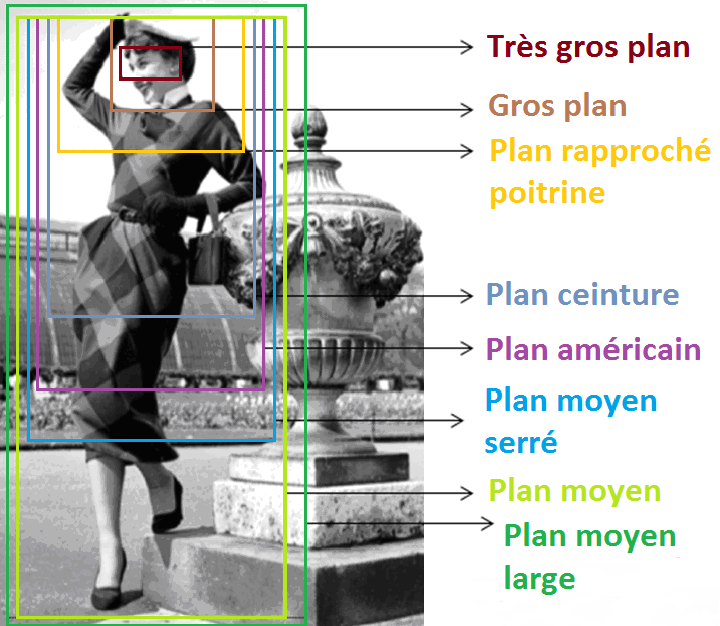
\includegraphics[width=0.5\textwidth]{./images/ValeurPlan-v1.png}
% \caption{Différentes valeurs de plan pour le cadrage d'un personnage à l'écran}
% \label{fig:cadrage}
% \end{figure}
%=============

Les amateurs quand à eux ignorent ces concepts et n'ont pas été initiés à ces pratiques. Ils ont donc besoin d'explications et d'illustrations pour comprendre les recommandations du réalisateur. 
Dans le cas du cadrage, une illustration graphique est d'autant plus pertinente. 
L'enjeu se situe donc dans la collaboration entre un prescripteur et un opérateur qui doivent s'accorder sur le contenu à produire malgré la différence de vocabulaire. 
% Un exemple des différences de présentation entre amateur et professionnel est illustré figure \ref{fig:prescription}.


% %%=============
% \begin{figure}[htb]
% \centering
% \includegraphics[width=0.3\textwidth]{./images/ShootingRecommandation-v1.png}
% \caption{Exemple de prescription de tournage à destination de professionnels (en haut) ou d'amateurs (en bas)}
% \label{fig:eda:prescription}
% \end{figure}
% %%=============


%%%%%%%%%%%%%%%%%%%%%%%%%%%%%%%%%%%%%%%%%%%%%%%%%%%%%%%%%%%%%%%%%%%%
\subsection{Besoins en modélisation}\label{sec:bm}
La mise en place d'une telle application nécessite de représenter le vocabulaire de la réalisation audiovisuelle dans toutes ses variations possibles et de le documenter suffisamment afin de le rendre compréhensible pour des novices. 
Cet objectif nous amène à considérer la construction d'une ressource termino-ontologique. L'ontologie permet de représenter les concepts partagés par les professionels de la réalisation audiovisuelle et la terminologie permet de capturer les différentes formes d'expression associées à ces concepts. 

La spécificité de notre problématique est de considérer la collaboration de communautés hétérogènes par leur degré de compréhension des concepts ou leur utilisation de la terminologie. 
Ceci nous amène à envisager la terminologie comme un moyen d'associer à des éléments ontologiques (concept, relation, instances) une chaîne lexicale ou des ressources média. 
Chaque chaîne ou ressource s'adresse en particulier à une communauté dont les membres partagent une capacité d'interprétation commune. 
Il n'existe donc plus une terminologie de référence par langue, mais des terminologies pour chaque communauté d'utilisateurs. 
On remarquera que notre acception de la terminologie sert bien à normaliser les pratiques linguistiques entre les membres d'une même organisation. 
En plus de cela, elle permet de fixer la manière de s'adresser à d'autres communautés.

Par ailleurs, les types de réalisations sont divers et nécessitent des concepts spécifiques pour être décrits. 
Une fiction se structure en séquences et en scènes alors que les documentaires ou magazines d'information se composent de sujets. 
La variabilité des types de contenu à filmer implique donc de pouvoir étendre le fond conceptuel initial pour représenter de nouveaux usages. 
De la même manière, la collaboration avec de nouveaux partenaires nécessite de pouvoir ajouter de nouvelles terminologies au fond conceptuel existant. 
Ontologie et terminologie doivent se gérer de manière indépendante. A partir de ces besoins, nous définissons maintenant les exigences en terme de modélisation. 

Nos besoins en modélisation peuvent être exprimés par les assertions suivantes:
\begin{enumerate}
	\item[(A1)] la variabilité des pratiques linguistiques des organisations et des communautés implique d'associer plusieurs termes à un même concept. 
	Il n'y a pas de choix des termes préférés par une communauté mais une \textit{correspondance} entre les termes d'une ou plusieurs communautés, quels que soient la langue et le code d'écriture utilisé.
	
	\item[(A2)] la variabilité de compréhension des communautés implique d'associer des explications (chaîne lexicale) ou des illustrations (ressource média) aux concepts afin d'en enrichir la \textit{documentation}. 
	
	\item[(A3)] la variabilité des cas de collaboration implique de pouvoir étendre la conceptualisation initiale ou la terminologie pour s'adapter à de nouvelles pratiques ou de nouvelles communautés. 
	Cela implique une gestion et une \textit{évolution} indépendante de l'ontologie et de la terminologie. 
\end{enumerate}


Dans le cas d'une demande de cadrage en plan américain, la demande est d'abord exprimée dans le jargon de la RTBF puis traduite dans le jargon de la VRT (plan américain pour la RTBF, plan 3/4 pour la VRT) [A1]. 
Ensuite, pour les amateurs, la terminologie est enrichie par des illustrations [A2]. Enfin, un nouveau concept de cadrage est ajouté (plan américain large ou plan moyen serré) [A3] en vue d'une nouvelle coopération avec la VRT. En plus de cela, le problème de la langue (français et flamand) s'ajoute à la question des jargons métiers. 



\section{Définitions des SOC (i)}\label{chap:defs}
%Distinguer entre terme et concept ; dictionnaire, thésaurus, ontologies etc.

\e{
L'objectif de cette section est de clarifier ce qui appartient au domaine de la  linguistique et ce qui relève du domaine conceptuel, en vue d'identifier les notions qui nous serviront à spécifier une solution au cahier des charges dressés dans la section précédente. 
La confusion qui nous intéresse concerne principalement la définition des ontologies par rapport à d'autres SOC tels ques les thésaurus, notamment du fait qu'on utilise parfois les mêmes langages pour les représenter.}

La définition des SOC proposée par \cite{Zacklad2010}, étend celle de \cite{Hodge2000} à \ciel{l'ensemble des formes d'écritures codifiées participant à la description documentaire primaire ou secondaire d'une situation}. 
L'ensemble défini par \citeauthor{Hodge2000} comprend ainsi tout type de :
\begin{liste}
	\item \e{liste de termes} (fichiers d'autorités, glossaires, dictionnaires, répertoires géographiques)
	\item \e{schème de classification/catégorisation} (vedettes-matières, taxonomie)
	\item \e{schème qui se structure par le types de relations qui unit ses membres} (thésaurus, réseaux sémantiques, ontologies). 
\end{liste}

À cela \citeauthor{Zacklad2010} souhaite ajouter des modes de description du contenu émergents ou plus faiblement codifiés comme par exemple les folksonomies. 
Les SOC qui nous intéressent en particulier sont les schèmes structurés par types de relations. 
% pourquoi ? 


\subsection{Thésaurus, terminologie, ontologie}
Dans cette section, nous nous reposerons majoritairement sur les définitions de \cite{bachimont:icc}. Concernant le thésaurus, l'auteur écrit :

\g{Thésaurus :} 
\ciel{
Une organisation de libellés linguistiques selon des relations d'hyperonymie et d'hyponimie. 
Les libellés sont également reliés par des relations dites d'association, qui sont de nature quelconque. 
Même si en pratique les libellés d'un thésaurus correspondent souvent à des termes du domaine, ce n'est pas nécessairement systématique.}

Cette définition situe clairement les thésaurus comme faisant partie du cadre de la linguistique. 
Il s'agit d'un ensemble de mots structurés et reliés suivant leur \e{signification}, c'est à dire leur sens normé ou commun à plusieurs contextes d'usage particuliers (à l'inverse du sens, qui lui varie suivant les usages, \cite{Roche2005}). 
\citeauthor{bachimont:icc} finit sa définition en comparant les mots issus d'un thésaurus aux termes. La distinction se joue à deux niveaux, la stabilité d'écriture du terme (niveau linguistique) et le fait qu'un terme renvoit à un concept (niveau conceptuel) : 

\g{Terme :} 
\ciel{
Une unité linguistique dont le signifié est un concept, c'est-à-dire un signifié normé. 
Le terme se manifeste linguistiquement par une stabilité et régularité de sa forme signifiante.
En particulier, un terme possède des contextes d'occurrence réguliers, obéissant à des canevas morpho-syntaxiques typiques. 
La détection de ces canevas est à la base des outils de détection des termes en corpus. 
Un terme peut posséder des variantes terminologiques.
Dans une optique normative, on détermine une forme préférée.}

Ainsi, plus qu'un repérage des mots (signifiant) utilisés dans un domaine donné, la terminologie s'attache à identifier les signifiés correspondants. 
Au-delà des débats sur les méthodes utilisées pour constituer les couples signifiant-signifié\footnote{L'approche \e{sémasiologique} (initiée par \cite{Bourigault1994}) s'appuie sur l'analyse linguistique d'un corpus de textes pour repérer les couplages signifiant-signifié ainsi que l'organisation conceptuelle sous-jacente. L'identification de ces \e{désignations} est ensuite validée par des experts du domaine. 
Dans une optique différente, l'approche \e{onomasiologique} prend comme appui la modélisation conceptuelle pour nommer ensuite les concepts. On parle alors de \e{dénominations} dont l'objectif est de refléter sans ambiguïté la structure conceptuelle dont elles sont issues.
Une critique faite à la première approche par \cite{Roche2006} est que les relations identifiées entre désignations sont purement linguistiques (hyper/hyponymie, méronymie etc.) et ne se rattachent pas à une structure conceptuelle. Ainsi, l'analyse de texte n'est qu'une première étape dans la constitution d'une terminologie, elle permet d'identifier les usages des mots, mais pas de les raccorder à des concepts. De même, la constitution du corpus va également grandement influer sur les résultats de l'analyse et pose alors un problème de réutilisabilité.}, on cherche à repérer la modélisation conceptuelle sous-jacente d'un domaine, de manière à pouvoir adosser chaque terme à un concept.
À noter que l'inverse n'est pas forcément valable, car il existe des concepts qui n'ont pas d'appelation usuelle et que l'on doit alors désigner par une phrase. 
Une autre conséquence de cette définition est que plusieurs mots peuvent être adossés au même concept.
Il devient alors important de pouvoir expliciter cette équivalence et éventuellement de spécifier un signifié préféré pour le terme.

Cette définition du terme préfigure ainsi la relation qu'entretient la terminologie avec l'ontologie pour \cite{bachimont:icc} : 

\g{Terminologie :} 
\ciel{un recensement et une organisation d'unités linguistiques à l'usage stabilisé et attesté, dont le signifié correspond à un concept du domaine.
La terminologie est l'organisation des termes du domaine.
La terminologie est la face linguistique de l'ontologie, qui en est le côté conceptuel. 
Il n'y a pas une stricte correspondance cependant entre ontologie et terminologie : si tout terme doit correspondre à un concept de l'ontologie, tout concept n'a pas forcément d'usage linguistique régulier attesté.}

De son côté, \cite[\S 2.4]{Roche2005} parle de manière similaire \ciel{[d']un système de termes reflétant une modélisation conceptuelle, [...] plus généralement dénommé \e{système notionnel} [qui] trouve sa raison d'être dans la façon dont nous appréhendons les objets du monde.}
\citeauthor{Roche2005} précise que si les systèmes notionnels ne relèvent pas de la linguistique, ils ne dépassent pas forcément le cadre d'une langue, sauf \ciel{pour des communautés de pratique dont les langues d'usage partagent la même conceptualisation du monde.}.
La distinction est ainsi faite entre les mots d'usage (qui peuvent être polysémiques) et les termes dont on spécifié une forme préférée (signifiant) et qu'on adosse à une signification (signifié normé).  

Concernant les particularismes qui peuvent exister dans chaque communauté, \citeauthor{Roche2005} propose de s'éloigner d'une vision purement normalisatrice. 
Ainsi, sur le plan linguistique, il est possible de rattacher les différents mots d'usages et de préciser leur contextes d'utilisation.
Sur le plan conceptuel, l'auteur propose de constituer des \gui{terminologies régionales} que l'on cherchera ensuite à mettre en correspondance. 




\paragraph{Ontologie}
Concernant les ontologies, nous nous limiterons aux définitions proposés dans le cadre de l'ingénierie des connaissances (IC). Les travaux de \cite{Charlet2002} nous rappelle qu'il existe de multiples définitions : 

Pour \cite{Gruber1993} : \ciel{Une ontologie est une spécification explicite d'une conceptualisation.}

 La définition proposée par \cite{Uschold1996} nous permet de préciser de quoi se compose une conceptualisation et en quoi une ontologie la spécifie : 

\ciel{Une ontologie implique ou comprend une certaine vue du monde par rapport à un domaine donné. Cette vue est souvent conçue comme
un ensemble de concepts -- e.g. entités, attributs, processus --, leurs définitions
et leurs interrelations. On appelle cela une conceptualisation. [...]
Une ontologie peut prendre différentes formes mais elle inclura nécessairement
un vocabulaire de termes et une spécification de leur signification. [...]
Une ontologie est une spécification rendant partiellement compte d’une conceptualisation.}

\citeauthor{Charlet2002} en conclut qu'une ontologie est une conceptualisation, c'est-à-dire un ensemble de concepts et de relations dont on cherche à normer la signification. 
Pour faire de la conceptualisation un objet informatique, il faut spécifier une théorie logique dotée d'un vocabulaire (les concepts et les relations), à la manière des travaux de \cite{Guarino1995}.

% Roche puis Babache
Pour \citeauthor{Roche2005}, une ontologie est équivalente au système notionnel des terminologies, d'où la relation forte établie par les chercheurs en IC : 

\ciel{définie pour un objectif donné et un domaine particulier, une ontologie est pour l'ingénierie des connaissances une représentation d'une modélisation d'un domaine partagée par une communauté d'acteurs. Objet informatique défini à l'aide d'un formalisme de représentation, elle se compose principalement d'un ensemble de concepts définis en compréhension, de relations et de propriétés logiques.} (\cite{Roche2005})

\citeauthor{Bachimont2000a} insiste sur le fait qu'on utilise une sémantique donnée (différentielle, référentielle, psychologique, distributionnelle, conceptuelle etc., \cite{bachimont:hdr}) pour établir la signification des concepts de l'ontologie. Chaque sémantique propose un point de vue particulier qui permet de faire correspondre une signification propre à chaque unité   : 

\ciel{une ontologie est la signature fonctionnelle et relationnelle, munie de sa sémantique, d'un langage formel de représentation et manipulation des connaissances.} (\cite{Bachimont2000a})

% ? différentes sémantiques 
Pour bien cerner les conséquences de cette définition, voici quelques sémantiques décrites par \cite{bachimont:hdr} qui se distinguent dans leur manière d'expliciter la signification d'une unité d'expression : 
\begin{liste}
	\item \e{sémantique différentielle} : la signification d'une unité consiste en l'identité et la différence par rapport aux autres unités linguistiques de la langue. On reste donc dans le cadre de la linguistique.
	\item \e{sémantique référentielle} : la signification d'une unité est l'objet auquel elle fait référence, dans un univers extralinguistique. Ici, on s'attache à une théorie %...
	\item \e{sémantique psychologique} : la signification d'une unité est la représentation mentale que l'on s'en fait. 
\end{liste}

% Au final, on construit un objet informatique en suivant une méthode de construction qui nous guide pour spécifier le comportement de l'ontologie. 

% RTO




\section{Méthode de construction d'ontologie}\label{chap:construction}
\subsection{Une méthode de construction d'ontologie}\label{sec:construction}
Nous avons défini dans la section précédente (\ref{sec:tto}) ce qu'est une ontologie,  présenté des exemples de sémantiques et montré comment il était possible de classifier ces ontologies suivant leur usage. 
Dans cette section, nous détaillons la méthode de construction d'ontologie \pc{Archonte} (\pc{arch}itecture for \pc{ont}ological \pc{e}laborating) proposé par \cite{Bachimont2000a}.
Cette présentation est aussi l'occasion de préciser l'importance crucuiale du choix d'une sémantique sur la construction d'une ontologie.

La méthode repose sur trois étapes successives qui aboutissent à une ontologie computationnelle, exprimée dans un langage opérationnel de représentation des connaissances et à partir duquel on peut effectuer des inférences. 
% Précisons maintenant les étapes de cette méthode ainsi que les résultats obtenus :
% \begin{liste}
Le point de départ de la méthodologie est constitué d'expressions linguistiques (signifiant) issues du domaine considéré.
L'intérêt de disposer d'un tel ensemble de traces linguistiques est qu'elles servent à exprimer des concepts (signifiés) ou des connaissances sur le monde. 
Ainsi, on se retrouve avec un corpus de candidats-termes dont la signification peut être source d'ambiguïtés et dont l'on cherche à clarifier l'interprétation.\\
% \end{liste}
% \begin{liste}

\g{[1.]} La première étape de cette méthode (aussi appelée \e{normalisation sémantique}) consiste à établir un \g{engagement sémantique}  qui précise la manière de mener l'interprétation des candidats-termes et de construire une première structure de connaissances. 
Pour cela, on fixe d'abord un contexte de référence, la tâche ou le problème qui a poussé à l'élaboration de l'ontologie, qui permet de cadrer l'interprétation des candidats-termes.

Ensuite, pour préciser l'interprétation on s'appuie sur la sémantique différentielle afin d'expliciter les différences et les similarités entre une notion et son voisinage direct (notion parente, notions soeurs) : 

	\ciel{
	La méthodologie que nous proposons ici repose sur l'organisation générale des unités en un réseau d'identités et de différences.
	Ce sont les propriétés structurelles de ce réseau qui permettent de contraindre l'interprétation des unités définies dans le réseau : la position d'une unité dans le réseau prescrit comment la comprendre et lui prescrit une signification qui pourra dès lors lui être associée, quel que soit le contexte où elle se rencontre.} (\cite[p.139]{bachimont:icc})

Cette caractérisation des notions par leur voisinage repose sur quatres relations à expliciter : 
\begin{liste}
	\item la \e{communauté avec le parent} (similarity with parent) : pourquoi la notion hérite des proprités de son parent.
	\item la \e{différence avec le parent} (difference with parent) : en quoi la notion est différente de son parent.
	\item la \e{différence avec les soeurs} (difference with siblings) : en quoi un notion est différentes de ses notions soeurs.
	\item la \e{communauté avec les soeurs} (similarity with siblings) : quelle est la propriété que partage les notion soeurs -- dont on distingue plusieurs valeurs exclusives, une par soeur.\\ 		
\end{liste}
% \end{liste}

Cette première étape aboutit à la construction d'un \g{arbre ontologique différentiel} qui structure un ensemble de notions de manière hiérarchique et non ambiguië par rapport à un contexte de référence.
Les candidats-termes sont structurés par des prescriptions interprétatives et deviennent ainsi des primitives de modélisation.\\

% \begin{liste}
\g{[2.]} L'\g{engagement ontologique} consiste à munir l'ontologie différentielle d'une sémantique formelle extensionnelle.
Rappelons que cette sémantique définit les concepts par leur extension, c'est-à-dire tous les individus qu'ils désignent parmi un ensemble de référence. 
Il s'agit donc de relier des primitives dotées d'une signification linguistique normalisée à des concepts désignant un ensemble de référents (ou individus).
Pour cela, il faut adjoindre à l'ontologie différentielle un modèle référentiel : 

	\ciel{
	l'ontologie référentielle obéit aux contraintes sémantiques de l'ontologie différentielle : [s]a structure arborescente se retrouve dans l'ontologie référentielle et lui donne son squelette.
	Chaque relation de spécialisation sémantique au niveau différentiel se traduit par une spécialisation d'extension au niveau référentiel.} (\cite[p.148]{bachimont:icc})

Ce changement de sémantique permet d'enrichir l'ontologie de nouveaux concepts et d'en modifier la structuration. 
En effet, on peut désormais avoir recours à des opérations ensemblistes (réunion, intersection, complémentaire) qui composent le sens des concepts et permettent ainsi de définir de nouveaux concepts.
L'ajout de ces \gui{concepts définis} modifie également la structure de l'ontologie, qui passe d'une arborescence à une structure en treillis, c'est-à-dire admettant l'héritage multiple. 
Par exemple, une primitive différentielle de \cd{mandat politique} spécialisée en concepts de \cd{député} et de \cd{maire} ne permet pas de représenter de double mandat.
Par contre, une définition extensionnelle permet de définir le concept de \cd{député-maire} simplement par l'intersection des extensions de ces concepts\footnote{Pour plus de détails sur cet exemple, se reporter à l'exemple donné par \cite[p.149]{bachimont:icc}}.
% \end{liste}

À l'issue de cette étape on obtient donc une \g{ontologie référentielle}, c'est-à-dire un treillis de concepts définis par une sémantique référentielle.\\

% \begin{liste}
\g{[3.]} L'\g{engagement computationnel} vise à doter les concepts de l'ontologie référentielle d'une signification en termes d'opérations informatiques.
Pour cela, il faut d'abord choisir un langage opérationnel de représentation des connaissances qui détermine l'expressivité et les opérations de calculs à disposition pour élaborer une version informatique de l'ontologie.
Nous présentons quelques uns de ces langages dans la section \ref{sec:onto-mc}.
La transposition dans un langage a des conséquences au niveau de l'expressivité et de la décidabilité du modèle.
% \end{liste}

Nous obtenons une \g{ontologie computationelle} qui est une version de l'ontologie référentielle exploitable informatiquement.


% \begin{liste}
% 	\item
% \end{liste}







\subsection{La validation en Ingénierie des Connaissances}\label{sec:valid-ic}
En suivant l'analyse proposée par \cite{Bachimont2004}, il en découle que  l'Ingénierie des Connaissances (IC) \ciel{exprime les connaissances d'un domaine dans un langage de modélisation et l'opérationnalise en un système}. 
En d'autres termes, la modélisation de l'IC porte sur les concepts utilisés par les gens de ce domaine pour penser et établir des connaissances sur le monde, mais pas directement sur le monde.
Ainsi, les modèles de l'IC n'ont pas pour vocation à \ciel{prédire quoi que ce soit sur le monde ni sur la connaissance}, mais plutôt d'\ciel{instrumenter le travail intellectuel, l'exercice de la pensée, le travail de la connaissance}. 
Dans cette perspective, \citeauthor{Bachimont2004} nous propose de théoriser l'IC comme \ciel{une ingénierie des inscriptions numériques des connaissances qui vise à instrumenter le travail cognitif associé à ces inscriptions}. 
        
Les inscriptions possèdent une double dimension ; \e{matérielle} (et donc manipulable par des techniques de calcul logique) ; \e{sémiotique} (et donc interprétable selon des conventions propres à une situation d'usage).  
En d'autres termes, le systèmes d'IC permet d'agir de manière prédictible sur les inscriptions de connaissances, ces actions produisant de nouvelles inscriptions qui donnent matière à penser à l'utilisateur. 
        
Il y a donc plusieurs éléments à valider en IC, les calculs qui seront faits sur les inscriptions (on teste le comportement du système informatique) puis l'interprétation de ces inscriptions (on évalue le gain apporté par le système et les inscriptions qu'il fournit à l'utilisateur selon une situation d'usage). 
La modélisation prise en charge par l'IC ne porte donc ni sur le monde, ni sur l'activité cognitive et ne peut être validée uniquement par le formalisme de ses inscriptions. 
        
Les inscriptions de connaissances doivent être considérées sous deux angles : d'un point de vue \e{nomographique} (on formalise la manipulation symbolique des inscriptions pour prévoir/définir le comportement du système) et \e{idiographique} (on décrit le sens des manipulations symboliques et des inscriptions produites par rapport aux normes, conventions, concepts du domaine).



% Au final, on construit un objet informatique en suivant une méthode de construction qui nous guide pour spécifier le comportement de l'ontologie. 

% RTO






\newpage
\section{Langages de représentation}\label{sec:mods}
\e{
  L'objectif de cette section est de présenter des langages de représentation qui permettent de structurer des documents textuels (\ref{sec:xml}) et de construire des systèmes de connaissances (SOC).
  Nous nous intéressons à deux types de SOC, les ontologies (\ref{sec:ln-onto}) et les vocabulaires structurés de type thésaurus (\ref{sec:thesaurus}).
  La vision du W3C joue un rôle fondamental dans la définition de ces langages et leur adoption en tant que standards par l'industrie et les communautés scientifiques engagées dans ces questions.
  L'idée d'un Web Sémantique, proposée par \cite{Berners-Lee2001}, constitue une nouvelle étape dans la manipulation automatique des données sur le Web, qui ajoute à l'objectif de représentation des structures, la formalisation de leur sémantique :} 

  \gui{
    The Semantic Web is not a separate Web but an extension of the current one, in which information is given well-defined meaning, better enabling computers and people to work in cooperation.}

  \e{
  Ainsi, la formalisation des connaissances permet d'orienter la manipulation et la rendre signifiante dans le cadre d'activités humaines.
  Nous étudions ainsi le langage RDF qui fournit un moyen d'annoter les ressources sur le Web (\ref{sec:rdf}), tandis que RDF-Schema (\ref{sec:rdfs}) permet de spécifier le vocabulaire utilisé sous la forme d'ontologie légère.
  OWL propose des axiomes de représentations plus expressifs permettant de construire des ontologies lourdes (\ref{sec:owl}). }



% \subsection{Langages de balisages }
\subsection{XML}\label{sec:xml}
eXtended Markup Language (XML) est un langage de structuration hiérarchique de texte par balise qui facilite sa manipulation par les machines, tout en restant lisible par des humains.
XML est défini formellement comme un sous-ensemble du langage \pc{Standard Generalized Markup Language} (SGML), conçu pour améliorer l'efficacité des parseurs et l'échange d'information sur le Web.
Il est devenu une recommandation du W3C en 1998. 

% aims to give a hierarchical structure to  text in a machine-, yet human-readable way. It is widely used to store or exchange information as it also supports Unicode.
% XML is formally defined as a Standard Generalized Markup Language's subset (SGML) designed to improve parser efficiency. Work on XML began in 1996 and it became a W3C Recommendation in early 1998.

\paragraph{Syntaxe}
Le balisage permet de créer des éléments qui encadrent du texte, de ce fait l'identifie et facilite ainsi sa manipulation.
Des attributs peuvent être ajoutés aux élements afin de donner une information sur leur contenu, sous la forme \cd{att1='val1'} séparés par des virgules.
Par exemple, \cd{xml:lang} permet de spécifier quel langage naturel a été utilisé pour écrire le texte encadré.
XML permet de plus d'imbriquer des éléments afin de créer une structure d'arbre représentant la structure dite \e{logique} ou \e{canonique} du document.
L'exemple suivant propose une synthèse de la syntaxe proposée par XML, en définissant l'élémént \cd{film} composé d'un sous-élément \cd{titre}.
Dans cet exemple, il s'agit de décrire le film \gui{Hook ou la revanche du capitaine Crochet}, mais en donnant le titre du film en Russe :
% This is achieved by adding mark-up elements that are easily noticed as they begin with '<' and end with a '>'. Mark-up elements are used to enclose unicode text, and give thus a mean to identify them and possibly to process it. As its name indicates, it is said extensible because we can define our own mark-up elements and writes a line like that:
% opening mark-up element       enclosing mark-up element
\begin{Verbatim}[fontsize=\small,formatcom=\color{black!70}]
<film>
  <titre xml:lang='ru'>Капитан Крюк</titre>
</film>
\end{Verbatim}

% Attributes can be defined for each mark-up element. 
% For instance, the xml:lang attributes indicates the natural language used to write the enclosed text. The \gui{1812 Overture} full title can be written like that:
% \begin{Verbatim}[fontsize=\small,formatcom=\color{black!70}]
% <title xml:lang='ru'>Торжественная увертюра 1812 года, Toržestvennaja uvertjura 1812 goda</title>
% <title xml:lang='fr'>Ouverture Solennelle, L'Année 1812, Op. 49</title>
% \end{Verbatim}

% \paragraph{Syntax}
% XML does not only enclose text with mark-up elements. It also enables to imbricate mark-up elements in such a way that the elements conforms to a tree structure. 

% \begin{Verbatim}[fontsize=\small,formatcom=\color{black!70}]
% <element>
% 	<sub-element>Example of text</sub-element>
% </element>
% \end{Verbatim}

% Other syntaxic rules have been defined to enables conforming parser to process XML file. Any file conspuing to these rules is said to be well-formed.

\paragraph{Schéma}
En plus de la syntaxe fournit par XML, il existe de nombreux langages de schéma\footnote{Nous citerons \gui{Document Type Defintion} (DTD) qui est très simple à prendre en main, mais peu expressif comparé à \gui{XML Schema} et \gui{Relax NG}.} qui permettent de modéliser des documents et de fournir des grammaires de structuration.
Ces schémas définissent des contraintes sur la structure des éléments, les attributs et les types de valeurs que l'on peut utiliser.
Un fichier XML qui se conforme aux contraintes d'un schéma particulier est dit \e{valide}.
Il existe donc deux types de contraintes pour les documents XML utilisant un schéma, la syntaxe de XML (qui les rend \e{bien formés}) et le schéma (qui les rend \e{valides}).

% XML permet également de créer
% Furthermore, if XML provides us with a syntax we also have the ability to makes purpose-specific XML-based mark-up languages – i.e. define constraints on structure, mark-up elements or even datatyping definition. Indeed, several schema languages exists and are used to encode documents or serialize text data according to a particular schema. XML files complying with a schema – i.e. conforming to the constraints defined in the schema – are said to be valid.


\paragraph{Espace de nom}
La création de schémas peut aboutir à des problèmes d'ambiguïtés entre des éléments homonymes. 
La définition d'un espace de nom (Namespace) permet de gérer ce problème en ajoutant un préfixe à chaque élément et attribut.
L'espace de nom propose ainsi un espace abstrait, identifié par une URI, qui résoud les problèmatiques de nommage d'éléments et permet ainsi de garder les spécificités de chacun des homonymes. 
On peut donc par exemple, redéfinir l'élément \cd{title} du Dublin Core en lui ajoutant le préfixe \cd{ex} correspondant à l'URI \cd{http://example.org} : 

% When creating schemas, ambiguity problems usually arise and namespace declaration can take care of that. Indeed, it provides an abstract container for XML elements and attributes and gives to their name a scope. As each namespace is identified by an URI, the ambiguity between identically named elements or attributes from differents namespace can be resolved. 

% Therefore, I can declare my own \gui{title} element and simultaniously use the \gui{DC Terms} property title. We show here a complete example with xml heading:
\begin{Verbatim}[fontsize=\small,formatcom=\color{black!70}]
<?xml version="1.0" encoding="UTF-8"?>
<ex:racine xmlns:dc="http://purl.org/dc/elements/1.1/"
    			 xmlns:ex="http://example.org">
	<dc:title>Hook</dc:title>
  <ex:title>Hook ou la revanche du capitaine Crochet</ex:title>
</ex:racine>
\end{Verbatim}
Dans cet exemple, dc:title correspond à l'élément désignant le titre courant, et ex:title correspond à l'élément désignant le titre long.


\subsubsection*{XML Schema}
Cette recommandation du W3C a été publiée en 2001, comme l'un des langages de schéma développé pour XML \parcite{Thompson2004}.
Souvent appellé XSD en référence à son suffixe de fichier '.xsd', le langage offre de nombreuses fonctionnalités : 
\begin{liste}
  \item Déclarer des imbrications (ordre et hiérarchie), des quantifications et des règles de nommage pour les éléments et attributs XML.
  \item Réutiliser des parties d'autres schémas grâce aux espaces de noms.
  \item Distinguer entre type simple (pas d'élément, ni d'attribut) ou des types complexes.
  \item La déclaration de types dérivés, en définissant des restrictions sur des types existants.
\end{liste}
% This W3C recommendation was published in 2001 and is one of several xml schema languages\footnote{We can cite, the old and very simple \gui{Document Type Defintion}(DTD) as well as the major rival of XML Schema, namely \gui{Relax NG}.}. It is often called XSD in reference to its files suffix – '.xsd'.

% XSD can define imbrication, quantification and naming rules for xml elements and attributes – in order to enable vocabulary and content model validation. XSD also supports namespace so parts of other schemas can be included or imported. 

\paragraph{Type de données}
Une des principales caractéristiques de XSD, et aussi une des plus critiquées, est l'utilisation de types de données (Datatype), qui peut s'appliquer sur les éléments ou les attributs pour contraindre le champ de valeur possible \parcite{Biron2004}.
Le problème soulevé étant que cette restriction ne peut se déclarer qu'à partir de la définition d'un type de données, soit par restriction, par liste de valeurs possibles, ou bien par union entre différents types de données.

% But one of the main and most criticized characteristic of XSD is DataType validation.
% It can be applied to elements or attributes to constraint their content.  DataType definition must use XSD primitive or derived datatypes – see the scheme for a detailled hierarchy. This dependence upon specific datatypes is the source of many criticism. 

% Derived datatypes can be built by restriction – of the permitted values set –, list – declaration of values –, or union – between several types. 
% As an complete example, we define a XSD schema describing \gui{MusicalOpus} as a list of XML elements named:
Voici un exemple de schéma XSD décrivant sommairement un film par une liste d'éléments XML : 
\begin{liste}
	\item Title: titre du film
	% \item Extent: length or duration – as a string
	\item Director: nom du réalisateur
	\item released: date de sortie du film (seulement l'année)
	% \item Performer: name of the performer
	% \item performed: date of performance – only the year
	\item writtenBy: nom de la personne ayant écrit une oeuvre dont le film propose une adaptation (attribut optionnel)
	\item DirectorNationality: nationalité du réalisateur (à partir d'une liste de valeur)
\end{liste}

Voilà le schéma XSD pour la description d'un Film:
\begin{Verbatim}[fontsize=\small,formatcom=\color{black!70}]
<?xml version="1.0" encoding="utf-8"?> 
<xs:schema elementFormDefault="qualified"   xmlns:xs="http://www.w3.org/2001/XMLSchema"> 
 <xs:element name="Film"> 
   <xs:complexType> 
     <xs:sequence> 
       <xs:element name="Title" type="xs:string" /> 
       <xs:element name="Director" type="xs:string" /> 
       <xs:element name="released" type="xs:gYear" /> 
       <xs:element name="writtenBy" type="xs:string" minOccurs="0"/>  
       <xs:element name="DirectorNationality"> 
         <xs:simpleType> 
           <xs:restriction base="xs:string"> 
             <xs:enumeration value="FR" /> 
             <xs:enumeration value="DE" /> 
             <xs:enumeration value="RU" /> 
             <xs:enumeration value="UK" /> 
             <xs:enumeration value="US" /> 
           </xs:restriction> 
         </xs:simpleType> 
       </xs:element> 
     </xs:sequence> 
   </xs:complexType> 
 </xs:element> 
</xs:schema> 
\end{Verbatim}
       % <xs:element name="Performer" type="xs:string" /> 
       % <xs:element name="performed" type="xs:gYear"/> 
% <xs:element name="Extent" type="xs:string" /> 

Voici un exemple de fichier XML dont le contenu est valide par rapport au schéma XSD précédent, le lien étant fait par l'attribut \cd{xsi:noNamespaceSchemaLocation} :
% And we provide a XML file which states that it conforms to the previous XSD scheme through a xsi:noNamespaceSchemaLocation attribute:
\begin{Verbatim}[fontsize=\small,formatcom=\color{black!70}]
<?xml version="1.0" encoding="utf-8"?> 
<Film xmlns:xsi="http://www.w3.org/2001/XMLSchema-instance" 
         xsi:noNamespaceSchemaLocation="Film.xsd"> 
  <Title>Hook ou la vengeance du capitaine Crochet</Title> 
  <Director>Steven Spielberg</Director> 
  <released>1991</released> 
  <writtenBy>James Matthew Barrie</conductedBy> 
  <DirectorNationality>US</DirectorNationality> 
</Film> 
\end{Verbatim}
%   <Extent>14:19</Extent>      
% <Performer>Minneapolis Symphony Orchestra</Performer> 
%   <performed>1954</performed> 














\subsection{Ontologie et modèle conceptuel}\label{sec:onto-mc}\label{sec:ln-onto}
\subsubsection{Resource Description Framework}\label{sec:rdf}
% \addcontentsline{toc}{subsubsection}{Resource Description Framework}
RDF est un modèle de graphe développé par le W3C \parcite{Manola2004}.
Il permet d'annoter et de relier des ressources sur le Web, de manière à les rendre manipulable par des agents logiciels.
Pour faciliter l'exploitation de ces ressources, RDF est doté d'une sémantique formelle propice à la réalisation d'inférences.

% The Resource  Description Framework (RDF) is an abstract model which is part of the W3C recommendations for the Semantic Web. 
% Let's just bring back to mind how \pc{Tim Berners-Lee} defined it to set RDF back into its context of creation: 

% \ciel{
% The Semantic Web is not a separate Web but an extension of the current one, in which information is given well-defined meaning, better enabling computers and people to work in cooperation.}

% Indeed, RDF aims to describe and link resources – and no more web pages – in a simple, all-purpose and machine-readable way. 
% The focus on software agents led to choose a formal semantic and provable inference. 
% Thus, such descriptions will foremost benefits to software agents which we'll be able to exploit, process and search into this web of linked data. 

\paragraph{Syntaxe}
L'annotation des ressources consiste à écrire des assertions sous la forme \e{Sujet --Prédicat--> Objet}.
Les sujets sont les ressources à annoter, les objets peuvent être soit une ressource, soit une valeur littérale.
Plusieurs assertions forment un graphe orienté dans lequel chaque \e{sujet/objet} est un noeud, et les prédicats (propriétés) sont des liens étiquettés.
RDF utilise les URI pour identifier ces ressources, propriétés et des valeurs littérales typées (par exemple, grâce aux types XSD).
RDF peut utiliser plusieurs types de sérialisations, comme RDF/XML, ou bien la Notation3 (N3).

L'exemple suivant annote la page Wikipédia du film \ciel{Hook} en précisant sa date de réalisation. L'annotation utilise des préfixes d'URI et une entité XML pour simplifier l'écriture de l'URI du type de données \cd{gYear} de XSD : 
\begin{Verbatim}[fontsize=\small,formatcom=\color{black!70}]
<?xml version="1.0"?>
<!DOCTYPE rdf:RDF [<!ENTITY xsd "http://www.w3.org/2001/XMLSchema#">]>
<rdf:RDF
  xmlns:rdf="http://www.w3.org/1999/02/22-rdf-syntax-ns#"
  xmlns:ex="http://example.org">
        <rdf:Description rdf:about="https://fr.wikipedia.org/wiki/Hook_ou_la_Revanche_du_capitaine_Crochet">
                <ex:released rdf:datatype="&xsd;gYear">1991</ex:released>
        </rdf:Description>
</rdf:RDF>
\end{Verbatim}

\paragraph{Grouper des ressources}
Lorsqu'une même ressource est le sujet de plusieurs assertions, la syntaxe de RDF nous impose de créer des noeuds intermédiaires (\e{blank node}).
De ce fait, ces noeuds ne sont pas référencés par une URI, mais utilise un système d'identification propre.

Ces groupes de ressources peuvent être typés pour définir la manière dont ses membres sont organisés.
Le type \cd{Collection} permet de définir des groupes clos (seul les membres cités sont compris dans le groupe), alors que le type \cd{Container} ne permet pas de clôturer l'appartenance à un groupe.
Ce dernier type propose trois sous-types qui organisent leurs membres de manière distincte : 

\begin{liste}
  \item Un sac (\cd{bag}) est un groupe non-ordonné qui peut contenir des doublons.
  \item Une séquence (\cd{seq}) est un groupe ordonné qui peut contenir des doublons. 
  \item Un type alternatif (\cd{alt}) est un groupe de valeur littérale ou de ressources alternatives.
\end{liste}

Par exemple, on peut déclarer une liste de noms alternatifs pour le titre du film \e{Hook} en utilisant le type \cd{alt} (anglais, français et le titre français du Canada) :
\begin{Verbatim}[fontsize=\small,formatcom=\color{black!70}]
wk:Hook         -- ex:Name -->    _blank_node_01
_blank_node_01  -- rdf:type -->   rdf:alt
_blank_node_01  -- rdf:li -->     'Hook' @en 
_blank_node_01  -- rdf:li -->     'Hook ou la Revanche du capitaine Crochet' @fr
_blank_node_01  -- rdf:li -->     'Capitaine Crochet' @fr-ca
\end{Verbatim}


\begin{table}[ht!]
   \begin{center}
    \begin{tabularx}{\textwidth}{|l|X|}
       \hline
    \gpc{Nom de la classe} & \gpc{Définition}\\ \hline\hline
    \cd{rdf:Statement} & La classe des assertions RDF.\\ \hline
    \cd{rdfs:Resource} & La classe de toute les ressources.\\ \hline
    \cd{rdfs:Class} & La classe de toutes les classes.\\ \hline
    \cd{rdf:Property} & La classe des propriétés RDF.\\ \hline
    \cd{rdfs:Literal} & La classe des valeurs littérales, chaîne de caractères, entiers etc.\\ \hline
    \cd{rdf:XMLLiteral} & La classe des valeurs littérales en XML.\\ \hline
    \cd{rdfs:Datatype} & La classe des types de données RDF.\\ \hline
    \cd{rdfs:Container} & The class of RDF containers.\\ \hline
    \cd{rdfs:ContainerMembershipProperty} & La classe container des propriétés d'appartenance à une groupe.\\ \hline
    \cd{rdf:Bag} & La classes container avec membres non-ordonnés.\\ \hline
    \cd{rdf:Seq} & La classes container avec membres ordonnés.\\ \hline
    \cd{rdf:Alt} & La classes container  avec membres alternatifs.\\ \hline
    \cd{rdf:List} & La classe des listes RDF.\\ \hline
    \end{tabularx}
    \caption{Liste des classes introduites par RDFS\label{tab:rdfs-classes}}
   \end{center}
\end{table}


\subsubsection{RDF Schema}\label{sec:rdfs}
% \addcontentsline{toc}{subsubsection}{RDF Schema}
RDFS a été développé pendant 6 ans par des groupes de travail du W3C, pour devenir une recommandation \parcite{Brickley2004}.
RDFS est un language permettant de définir des vocabulaires de descriptions de ressources, proche des ontologies.
Comme RDF, RDFS suit une approche minimaliste qui réduit l'expressivité du langage pour faciliter son exploitation, contrairement à OWL qui lui rajoute certains raffinements.

\paragraph{Ressource, Classe, Propriété}
RDFS définit des classes de ressources (voir la Table \ref{tab:rdfs-classes}), identifiés par des URI, décrits par des propriétés (voir la Table \ref{tab:rdfs-properties}) et associés avec un ensemble d'instances (l'extension de la classe). 
Les classes, comme les propriétés, sont hiérarchisées par la primitive \cd{rdfs:subClassOf} (\cd{subPropertyOf} pour les propriétés).
Une des particularités de \cd{rdfs:class}, comme de \cd{rdfs:property}, est de s'accepter comme des instances, ce qui explique leur présence dans la liste des classes et de propriétés.

Les propriétés définissent des liens entre ressources, l'une étant le sujet de l'assertion, l'autre l'objet.
La déclaration des propriétés utilise les propriétés \cd{rdfs:domain} et \cd{rdfs:range} pour contraindre la classe de ressources pouvant être utilisée comme sujet (le domaine) et objet d'une assertion (la portée).
Remarquons également que les propriétés suivantes correspondent plus à une documentation des vocabulaires construits par RDFS, qu'à une anntotation de ressources : \cd{rdfs:label}, \cd{rdfs:comment}, \cd{rdfs:seeAlso}, \cd{rdfs:isDefinedBy}.



% 7.3.2.a  Property List
\begin{table}[ht!]
   % \begin{center}
		\begin{tabularx}{450pt}{|l|X|r|l|}
		   \hline 
       \gpc{Nom de la propriété} & \gpc{Définition} & \gpc{Domaine} & \gpc{Portée} \\ \hline\hline
\cd{rdf:type} & Le sujet est une instance de la classe. & \cd{rdfs:Resource} & \cd{rdfs:Class} \\ \hline
\cd{rdfs:subClassOf} & Le sujet est une sous-classe de la classe. & \cd{rdfs:Class} & \cd{rdfs:Class} \\ \hline
\cd{rdfs:subPropertyOf} & Le sujet est une sous-propriété de la propriété. & \cd{rdf:Property} &\cd{rdf:Property} \\ \hline
\cd{rdfs:domain} & Le domaine d'une propriété (la classe de ressources pouvant être sujet). & \cd{rdf:Property} & \cd{rdfs:Class}\\ \hline
\cd{rdfs:range} & La portée d'une propriété (la classe de ressources pouvant être objet) & \cd{rdf:Property} & \cd{rdfs:Class}\\ \hline
\cd{rdfs:label} & Une étiquette lisible par des humains. & \cd{rdfs:Resource} & \cd{rdfs:Literal} \\ \hline
\cd{rdfs:comment} & Une description de la ressource sujet. & \cd{rdfs:Resource} & \cd{rdfs:Literal}\\ \hline
\cd{rdfs:member} & Une ressource membre de la ressource sujet. & \cd{rdfs:Resource} & \cd{rdfs:Resource}\\ \hline
\cd{rdf:first} & Le premier élémént d'une liste RDF. & \cd{rdf:List} & \cd{rdfs:Resource}\\ \hline
\cd{rdf:rest} & Le reste d'une liste RDF (les éléments après le premier). & \cd{rdf:List} & \cd{rdf:List}\\ \hline
\cd{rdfs:seeAlso} & Des informations complémentaires sur le sujet. & \cd{rdfs:Resource} &\cd{rdfs:Resource}\\ \hline
\cd{rdfs:isDefinedBy} & La définition de la ressource sujet. & \cd{rdfs:Resource} & \cd{rdfs:Resource}\\ \hline
\cd{rdf:value} & Propriété idiomatique utilisée pour la définition de valeurs structurés (Container etc.) & \cd{rdfs:Resource} & \cd{rdfs:Resource}\\ \hline
\cd{rdf:subject} & Le sujet d'une assertion RDF. & \cd{rdf:Statement} & \cd{rdfs:Resource}\\ \hline
\cd{rdf:predicate} & Le prédicat (propriété) d'une assertion RDF. & \cd{rdf:Statement} & \cd{rdfs:Resource}\\ \hline
\cd{rdf:object} & L'objet d'une assertion RDF. & \cd{rdf:Statement} & \cd{rdfs:Resource}\\ \hline
		\end{tabularx}
		\caption{Class list \label{tab:rdfs-properties}}
   % \end{center}
\end{table}

% Eventually, observe these four properties that appear more like annotation than property defining resource: \cd{rdfs:label}, \cd{rdfs:comment}, \cd{rdfs:seeAlso}, \cd{rdfs:isDefinedBy}.





\subsubsection{Ontology Web Language}\label{sec:owl}
% \addcontentsline{toc}{subsubsection}{Ontology Web Language}
OWL est un langage de représentation des connaissances visant à construire des ontologies pour le Web \parcite{Bechhofer2004}.
Le travail sur le langage a débuté en 2001 à partir des travaux sur DAML+OIL initiés conjointement par le \pc{Defense Advanced Research Projects Agency} (DARPA) et le le projet \pc{Information Society Technologies} (IST) de l'Union Européenne \parcite{Connolly2001}.

OWL repose sur RDF et une syntaxe XML et définit ses primitives par extension des classes et propriétés RDF/RDFS, notamment en ajoutant des contraintes de cardinalité ou de comparaison sur les déclarations de classes et de propriétés.
En comparaison de RDF/RDFS, dont la sémantique se rapproche de celle des graphes conceptuels, OWL est doté d'une sémantique en logique de description.
OWL permet ainsi de développer des ontologies informatiques exploitables par des outils de raisonnement.
Cependant, afin de couvrir un plus grand nombre de cas d'usage, OWL définit trois sous-langages dont l'expressivité, et donc l'efficacité computationnelle, varie. 
Chaque sous-langage est un sous-ensemble de ses prédécesseurs, ce qui implique que toute représentation en \pc{OWL Lite} est valide en \pc{OWL-DL}, et de même entre \pc{OWL-DL} et \pc{OWL Full}.

\begin{liste}
  \item \pc{OWL Full} a été conçu comme un sur-ensemble de RDF/RDFS de manière à être le plus compatible avec lui, au prix de la décidabilité.
  Par exemple, \pc{OWL Full} est la seule version de OWL qui accepte que tout élément d'une ontologie soit considéré comme un individu (même pour les classes et les propriétés).

  \item OWL-DL dispose des mêmes primitives que \pc{OWL Full}, mais leur usage est plus contraint de manière à assurer complétude computationnelle (toutes les inférences sont calculables) et décidabilité (tous les calculs finissent en un temps fini).

	\item \pc{OWL Lite} est le plus simple, le moins expressif des sous-langage.
  Il a été conçu pour formaliser des ontologies peu complexe et favoriser la vitesse de raisonnement.	
\end{liste}
% Each level is a sub-level from its predecessor, that is every legal ontology or valid conclusion expressed in \gui{OWL Lite} is a legal ontology or respectively a valid conclusion in \gui{OWL-DL} and so on between \gui{OWL-DL} and \gui{OWL Full}. 

Une ontologie OWL est un ensemble \e{classes} et de \e{propriétés} organisé hiérarchiquement et éventuellement associé à une base de faits, c'est-à-dire des \e{instances} de ces classes et des assertions les reliant.
La Table \ref{tab:owl-class} présente l'ensemble des axiomes s'appliquant aux classes OWL. 
Les cases en gris clair indiquent les axiomes qui s'appliquent à \pc{OWL Lite} sous conditions, et les cases en gris foncé, les axiomes qui ne sont pas disponibles dans \pc{OWL Lite} (mais bien dans OWL-DL et \pc{OWL Full}).
On distingue en particulier, les axiomes qui permettent de déclarer une nouvelle classe, éventuellement en apposant des restrictions ou en combinant d'autres classes, de ceux qui participent à sa définition, notamment en rapport avec les autres classes de l'ontologie.
À cela, il faut ajouter l'axiome RDFS \cd{rdfs:subClassOf}.
% Il est important de noter que toutes les classes sont des sous-classe de la superclasse \cd{owl:Thing}.


\begin{table}[ht!]
    \begin{tabularx}{\textwidth}{|p{3cm}|X|r|}
       \hline
     \multicolumn{2}{|X|}{\gpc{Axiomes de déclaration de classe}} & \gpc{Primitive}\\ \hline\hline
    
    \multicolumn{2}{|p{11cm}|}{\e{Déclaration simple} en utilisant une URI.} & \cd{owl:class} \\ \hline
    
    \rowcolor{lightgray} 
    \multicolumn{2}{|p{11cm}|}{\e{Déclaration par énumération} exhaustive de l'extension de classe (instance), par exemple en utilisant les primitives RDFS de groupage.} & \cd{owl:oneOf} \\ \hline
    

    \multirow{3}{3cm}{\e{Combinaison booléenne}} & opérateur logique AND & \cd{owl:intersectionOf}  \\ \cline{2-3}
    & opérateur logique OR & \cellcolor{lightgray} \cd{owl:unionOf}  \\ \cline{2-3}
    & opérateur logique NOT & \cellcolor{lightgray} \cd{owl:complementOf} \\ \hline
    

    \multirow{7}{3cm}{\e{Restriction sur les propriétés}} & \multirow{2}{8cm}{en désignant une classe (\pc{OWL Lite}) ou bien un types de données} & \cellcolor{black!10} \cd{owl:allValuesFrom} \\ \cline{3-3}
    & & \cd{owl:someValuesFrom} \\ \cline{2-3}
    & en désignant des instances ou des valeurs littérales & \cellcolor{lightgray} \cd{owl:hasValue} \\ \cline{2-3}
    & \multirow{3}{8cm}{en définissant des cardinalités (0..1 pour \pc{OWL Lite})}
    & \cellcolor{black!10} \cd{owl:maxCardinality} \\ \cline{3-3}
    & & \cellcolor{black!10} \cd{owl:minCardinality} \\ \cline{3-3}
    & & \cellcolor{black!10} \cd{owl:cardinality} \\ \hline\hline


    \multicolumn{2}{|X|}{\gpc{Axiomes de définition de classe}} & \gpc{Primitive}\\ \hline\hline
    \multicolumn{2}{|p{11cm}|}{\e{Spécialisation} en désignant une classe mère dont l'extension contient l'extension de la classe fille.} & \cd{owl:subClassOf}\\ \hline
    \multicolumn{2}{|p{11cm}|}{\e{Équivalence} entre classes (extension équivalente)} & \cd{owl:equivalentClass}\\ \hline
    \multicolumn{2}{|p{11cm}|}{\e{Disjonction} entre les extensions de classes} & \cellcolor{lightgray} \cd{owl:disjointWith}\\ \hline

    \end{tabularx}
    \caption{Axiomes de classe en OWL\label{tab:owl-class}}
\end{table}

OWL distingue quatre types de propriétés, qui doivent être mutuellement disjointes lorsqu'on utilise OWL-DL :
\begin{liste}
	\item \cd{owl:DatatypeProperty} associe des valeurs littérales à une instance.
	\item \cd{owl:ObjectProperty} définit des relations entre des instances.
	\item \cd{owl:AnnotationProperty} associe n'importe quelle valeur ou ressource à une instance dans un but de documentation de l'ontologie. 
  En effet, ces propriétés ne seront pas traités par les raisonneurs.
  En OWL-DL, il est impossible de définir des restrictions ou des spécialisations sur ces propriétés.
	\item \cd{owl:OntologyProperty} est utilisée pour l'importation d'ontologie et documenter le développement (par version) de l'ontologie.
	En OWL-DL, ces propriétés partagent les mêmes contraintes que les propriétés d'annotation.
\end{liste}

Ces propriétés sont définies par l'intermédiaire d'axiomes RDFS, pour déclarer le domaine (\cd{rdfs:domain}) et la portée (\cd{rdfs:range}) ou encore une propriété mère (\cd{rdfs:subPropertyOf}).
À cela, OWL ajoute des axiomes permettant d'établir l'équivalence entre deux propriétés (\cd{owl:equivalentProperty}) ainsi que d'autres propriétés algébriques qui affine la formalisation des définitions : 
\begin{liste}
  \item \cd{owl:TransitiveProperty}: P(X,Y) et P(Y,Z) implique P(X,Z). 
  Par eXemple, si X est près de Y et Y est près de Z, alors X est près de Z.
  \item \cd{owl:SymetricProperty}: P(X,Y) si et seulement si (ssi) P(Y,X).Si X est près de Y, alors Y doit être près de X.
  \item \cd{owl:FunctionalProperty}: P(X,Y) et P(X,Z) implique Y = Z. 
  La propriété possède une seule valeur pour chaque individu sur laquelle elle s'applique.
  \item \cd{owl:InverseFunctionalProperty}: P(Y,X) et P(Z,X) implique Y = Z.
  \item \cd{owl:InverseOf}: P1(X,Y) ssi P2(Y,X). 
  Si X est pèreDe Y, alors Y est filsDe X, donc les propriétés pèreDe et filsDe sont inverses.
\end{liste}

Les propriétés d'annotation utilisées sont celles de RDFS, plus la propriété \cd{owl:versionInfo} qui permet de documenter la version actuelle de l'ontologie.
Les propriétés d'ontologies (\cd{owl:priorVersion}, \cd{owl:backwardCompatibleWith}, \cd{owl:incompatibleWith}) permettent de documenter l'ontologie en précisant sa relation avec d'autres versions (représentées par des instances de instance de \cd{owl:Ontology}).
Les propriétés \cd{owl:DeprecatedClass} et \cd{owl:DeprecatedProperty} désignent les classes ou propriétés qui sont maintenues dans l'ontologie pour des raisons de compatibilité, mais ne sont pas susceptibles d'être utilisées dans les futures versions.

% \paragraph{Property declaration}
% We take as an example the definition of creation relationships on two different level of specialisation. 
% First, a \gui{createdBy} relation between a \gui{Person} and an \gui{Opus}. 
% Second, a music related \gui{composedBy} relation, involving a \gui{Composer} and a \gui{MusicalOpus}.

% Class declaration:
% \begin{Verbatim}[fontsize=\small,formatcom=\color{black!70}]
% <owl:Class rdf:ID='Composer'>
% 	<rdfs:subClassOf rdf:resource='Person' />
% </owl:Class>
% <owl:Class rdf:ID='Opus' />
% <owl:Class rdf:ID='MusicalOpus'>
% 	<rdfs:subClassOf rdf:resource='Opus' />
% </ow:Class>
% \end{Verbatim}

% Property declaration:
% \begin{Verbatim}[fontsize=\small,formatcom=\color{black!70}]
% <owl:ObjectProperty rdf:ID='createdBy'>
% 	<rdfs:domain rdf:resource='Opus' />
% 	<rdfs:range rdf:resource='Person' />
% </owl:ObjectProperty>
% <owl:ObjectProperty rdf:ID='composedBy'>
% 	<rdfs:domain rdf:resource='MusicalOpus' />
% 	<rdfs:range rdf:resource='Composer' />
% 	<rdfs:subPropertyOf rdf:resource='createdBy />
% </owl:ObjectProperty>
% \end{Verbatim}
% Note the use of rdfs:domain, rdfs:range, rdfs:subPropertyOf and rdfs:subClassOf properties within OWL statements.

% Now, if we want to take advantage of Property restrictions to define our \gui{Composer} class, we can state for instance that \gui{Composer} individuals are precisely those \gui{Person} individuals who have \gui{composed} at least one \gui{MusicalOpus}. 
% This lead us to write the following declaration: 
% \begin{Verbatim}[fontsize=\small,formatcom=\color{black!70}]
% <owl:Class rdf:ID='Composer'>
%   <rdfs:subClassOf>
%     <owl:intersectionOf rdf:parseType='Collection'>
%       <owl:Class rdf:ID='Person' />
%       <owl:Restriction>
%         <owl:onProperty rdf:resource='composedBy' />
%         <owl:minCardinality rdf:datatype='\&xsd;nonNegativeInteger'>1</owl:minCardinality>
%       </owl:Restriction>
%     </owl:intersectionOf >
%   </rdfs:subClassOf>	
% </owl:Class>
% \end{Verbatim}
% Note that the intersectionOf property requires a list of Classes declarations which can be given either by owl:Class or owl:Restriction – which is defined as a sub-class of owl:Class. 


% \paragraph{Individual}
Les ontologies OWL peuvent également contenir des individus, c'est-à-dire des instances de classes, décrits par l'usage de propriétés.
Ces individus sont identifiés par des URI, comme dans RDF/RDFS. 
Trois axiomes OWL permettent de définir des individus par leurs relations aux autres : 
\begin{liste}
  \item \cd{owl:sameAs} déclare deux URI comme faisant référence au même individu, permettant ainsi de fusionner leur définition et les conclusions qu'on a pu en tirer.
  \item \cd{owl:differentFrom} déclare explicitement deux URI comme se référant à des individus distincts.
  \item \cd{owl:AllDifferent} permet de déclarer que tous les individus d'une liste sont distincts.
\end{liste}
% Ontology is not only about Classes and Properties, it enables us to state some facts about individuals. In order to describe them, we state them as Class instance, make use of Property or assert facts about their individuality. 
% Let's use our previous ontology description to decribe \gui{Tchaikovsky} and the \gui{1812 overture}.
% \begin{Verbatim}[fontsize=\small,formatcom=\color{black!70}]
% <Person rdf:ID='Tchaikovsky' />
% <MusicalOpus rdf:ID='1812_Overture'>
% 	<composedBy rd:resource='Tchaikovsky' />
% </MusicalOpus>
% \end{Verbatim}

% From this description, we can entail that:
% \gui{Tchaikovsky} is not only a \gui{Person}, it is also a \gui{Composer} because he composed the \gui{1812 overture}. As he composed it, we can also say that he has \gui{created} it. 

% As OWL is a web language, it has rejected the \gui{unique name} assumption and hence need to deal with identity uniqueness – and thus URI reference. In order to do so, three constructs have been defined:
 



% Now, to demonstrate the use of sameAs property and to refer to our information sample, we define several \gui{Tchaikovsky} individuals with different spelling. Then, we declare several MusicalOpus, \gui{Cappricio italien} and «\verb?Ромео и Джульетта?» which is the russian spelling for \gui{Romeo and Juliet}.

% \begin{Verbatim}[fontsize=\small,formatcom=\color{black!70}]
% <Person rdf:ID='Tchaïkovski' xml:lang='fr' />
% <Person rdf:ID='Чайкoвский' xml:lang='ru' />

% <MusicalOpus rdf:ID='Capriccio_italien' xml:lang='fr'>
% 	<composedBy rd:resource='Tchaïkovski' />
% </MusicalOpus>
% <MusicalOpus rdf:ID='Ромео и Джульетта' xml:lang='ru'>
% 	<composedBy rd:resource='Чайкoвский' />
% </MusicalOpus>
% \end{Verbatim}
% If we change the first statements by:
% \begin{Verbatim}[fontsize=\small,formatcom=\color{black!70}]
% <Person rdf:ID='Tchaïkovski' xml:lang='fr'>
% 	<owl:sameAs rdf:resource='Tchaikovsky'/>
% </Person>
% <Person rdf:ID='Чайкoвский' xml:lang='ru'>
% 	<owl:sameAs rdf:resource='Tchaikovsky'/>
% </Person>
% \end{Verbatim}
% We can entail that there are the same person and that he has composed all three \gui{MusicalOpus} described. 





\paragraph{Discussion}
OWL, notamment dans ces versions OWL-DL et \pc{OWL Full} enrichit fortement l'expressivité des modélisations par rapport à RDF/RDFS, notamment du fait des définitions de propriétés avec des propriétés algébriques, et de la déclaration de classes par ajout de restrictions ou de combinaisons booléenne.
Les primitives de OWL permettent de documenter les concepts a minima, grâce à l'apposition d'étiquettes multilingues, à l'ajout de définition et au renvoi vers des ressources externes [\g{$\delta_2$ : documentation}]. 
Les propriétés d'ontologie permettent de documenter son évolution et faciliter sa prise en main par ses utilisateurs.
De plus, la possibilité d'importer des ontologies et d'utiliser des espaces de noms (via les URI) permet l'intégration d'autres ontologies, qu'on peut ensuite aligner pour fusionner les connaissances [\g{$\delta_3$ : gestion, évolution}].
Pour autant, OWL ne permet pas d'associer un thésaurus multi-jargon à la conceptualisation modélisée, car les étiquettes sont des valeurs littérales, et non des objets que l'on peut organiser hiérarchiquement [\g{$\delta_1$ : multi-jargon}].
De ce fait, OWL n'est pas suffisant pour satisfaire à tous nos besoins de modélisations (\ref{sec:bm}).
La section suivante examine donc des formalismes de représentation de vocabulaire structuré.
L'objectif étant de pouvoir représenter l'ontologie en OWL et d'intégrer des vocabulaires à cette ontologie via un autre formalisme.








\subsection{Thésaurus et vocabulaire structuré}\label{sec:thesaurus}
\subsubsection{Simple Knowledge Organization System}\label{sec:skos}
% \addcontentsline{toc}{subsubsection}{Simple Knowledge Organization System}
\e{
SKOS est un langage de représentation de vocabulaires structurés et de thésaurus qui repose sur RDF et OWL. 
Son objectif est de représenter tout type de SOC en vue de le publier sur le web de données,  liées et ouvertes (Linked Open Data). 
En témoigne les travaux et méthodes de conversion proposés par \cite{Summers2008} ou \cite{VanAssem2006} et les applications de gestion de thésaurus développés autour de SKOS, comme celle de \cite{Schandl2010}.
On notera que l'objectif de publication semble pousser vers une représentation minimale mais extensible de SOC déjà construits.
}

\paragraph{Concept et Etiquette}
SKOS centre son modèle sur les concepts (\cd{skos:Concept}) et considère les étiquettes comme des propriétés de ces derniers. 
On distingue trois types d'étiquettes: 
\begin{liste} 
	\item Les étiquettes préférées (\cd{skos:prefLabel}) qui sont uniques par langue et servent de référence.
	\item Les étiquettes alternatives (\cd{skos:altLabel}) qui servent de synonymes pour l'étiquette de référence. 
	\item Les étiquettes cachées (\cd{skos:hiddenLabel}) qui servent à la récupération d'erreurs de frappes les plus courantes. 
\end{liste}
Chacune de ces propriétés est formalisée comme une instance de \cd{owl:Anno\-tationProperty}, ce qui permet de l'attacher dans les faits à tout type d'éléments ontologiques, et pas seulement à des concepts. 
Les valeurs lexicales portées par ces étiquettes sont formalisées comme des \cd{rdf:PlainLiteral}, ce qui permet de spécifier la langue et l'alphabet utilisés. 
Par exemple, la chaîne "higashi"@ja-Latn correspond à un mot japonais écrit avec l'alphabet latin.

\paragraph{Documentation}
Différentes notes de documentation existent afin de :
\begin{liste}
	\item Définir un concept (\cd{skos:definition}), expliciter son contexte d'usage (\cd{skos:scopeNote}) ou donner des exemples (\cd{skos:example}).
	\item Spécifier l'historique de sa signification (\cd{skos:historyNote}), les changements effectués (\cd{skos:changeNote}) ou à faire (\cd{skos:editorialNote}).
\end{liste}
L'ensemble de ces notes est défini comme une spécialisation de \cd{skos:note}, formalisé comme une \cd{owl:annotationProperty}. 
De cette manière, les notes peuvent servir à porter de la documentation écrite (comme les étiquettes), pointer vers des ressources RDF ou des documents identifiés par une URI. 
Cela permet ainsi de prévoir l'extension de ces notes à des besoins plus spécifiques.


\paragraph{Groupes et relations entre Concepts}
Les concepts peuvent être regroupés dans des schémas conceptuels (\cd{skos:\-ConceptScheme} et relation \cd{skos:inScheme}) et structurés par différentes relations:
\begin{liste}
	\item Des relations de structuration hiérarchiques (\cd{skos:broader}, \cd{skos:na\-rrower}) ou associatives (\cd{skos:related})
	\item Des relations de correspondances entre concepts de schémas différents, soit une relation d'équivalence exacte (\cd{skos:exactMatch}), une équivalence approximative (\cd{skos:closeMatch}), des relations hiérarchiques (\cd{skos:broadMatch}, \cd{skos:narrowMatch}) ou associative \cd{skos:rela\-ted\-Match}).
\end{liste}



\paragraph{Exemple de représentation} 
Pour illustrer l'utilisation de SKOS, nous reprendrons le scénario présenté dans notre cahier des charges fonctionnels (\ref{sec:cdcf}). 
Il s'agit de représenter deux termes de jargons correspondant au même concept de cadrage.
En effet, les deux organisations ont décidé de lier la définition de leur concept malgré leur usage d'étiquettes différent. 
Ceci se reflète par la mise en relation explicite de ces concepts (\cd{skos:exactMatch}) et leur incorporation dans des schèmes différents (\cd{skos:inScheme}).
Par ailleurs, la VRT utilise des étiquettes cachées pour gérer l'utilisation d'abréviations par les utilisateurs écrivant leurs requêtes. 
Afin de satisfaire aux besoins des amateurs, on rajoute également une illustration graphique ainsi qu'une définition :
\begin{Verbatim}[fontsize=\small,formatcom=\color{black!70}]
//====== CONCEPTS ======//
<PlanAmericain> rdf:type skos:Concept ; 
  skos:prefLabel "Plan américain"@fr ;
  skos:prefLabel "American shot"@en
  skos:altLabel "Plan 3/4"@fr ;
  skos:altLabel "Medium-close shot"@en ;
  skos:inScheme   <RTBF-Scheme> ;
  skos:inScheme   <AV-Scheme> ;
  skos:example ex:PlanAmericain.png ;                               //Illustration//
  skos:definition "plan coupant les personnages à mi-cuisse"@fr ;   //Définition//
  skos:exactMatch <Plan34> .
   
<Plan34> rdf:type skos:Concept ;
  skos:prefLabel "3/4 shot"@en
  skos:prefLabel "Plan 3/4"@fr ;
  skos:altLabel "Medium-close shot"@en ;
  skos:hiddenLabel "mcs"@en ;                                       //Abréviations//
  skos:hiddenLabel "m.c.s."@en ;
  skos:example ex:PlanAmericain.png ;                               //Illustration//
  skos:definition "shows a character from head to the middle of the leg"@en ;
  skos:inScheme   <AV-Scheme> ;
  skos:inScheme   <VRT-Scheme> .
\end{Verbatim}



\paragraph{SKOS-XL}\label{sec:skos-xl}
SKOS-XL est une extension de SKOS développée courant 2008 pour proposer une modélisation alternative au vocabulaire de base et favoriser des extensions plus fines. 
Dans SKOS-XL les termes ne sont plus portés par les concepts mais deviennent des éléments à part entière (\cd{skosxl:Label}). 

Les relations d'attachement entre termes et concepts sont analogues aux attributs de SKOS mais les formalisent comme des instances de \cd{owl:objectProperty}. 
Le domaine de ces relations n'est pas défini ce qui permet de les associer à n'importe quelle ressource RDF, et donc en particulier aux concepts SKOS mais également à des ConceptScheme. 
Si cette dernière possibilité permet de créer des groupes de termes, elle introduit une confusion sur la sémantique des ConceptScheme.
Est-ce un groupe de concepts, de termes ou bien de triplets ? 
Les étiquettes portent une seule chaîne lexicale avec les mêmes possibilités que pour SKOS grâce à l'attribut \cd{skos:literalForm}. 
L'indépendance des étiquettes permet également de spécifier des relations entre eux comme la synonymie, la traduction, etc. \cite{Pastor2009a}. 
Cette possibilité est ouverte par la relation générique \cd{skosxl:labelRelation}. 


% REVOIR les termes par rapport à l'exemple de SKOS
\begin{Verbatim}[fontsize=\small,formatcom=\color{black!70}]
//====== CONCEPTS ======//
C-PlanAmericain rdf:type skos:Concept ; 
  skosxl:prefLabel <T-PlanAmericain> ;
  skosxl:prefLabel <T-AmericanShot> ;
  skosxl:altLabel <T-Plan34> ;
  skosxl:altLabel <T-MCShot> ;
  skos:example ex:PlanAmericain.png ;                               //Illustration//
  skos:definition "plan coupant les personnages à mi-cuisse"@fr ;   //Définition//
  skos:inScheme   <RTBF-Scheme> ;
  skos:inScheme   <AV-Scheme> ;
  skos:exactMatch <C-Plan34> .

C-Plan34 rdf:type skos:Concept ;
  skosxl:prefLabel <T-Plan34> ;
  skosxl:prefLabel <T-34Shot> ;
  skosxl:altLabel <T-MCShot> ;
  skosxl:hiddenLabel <T-MCS> ;                                      //Abréviations//
  skosxl:hiddenLabel <T-M-C-S> ;
  skos:example ex:PlanAmericain.png ;                               //Illustration//
  skos:definition "shows a character from head to the middle of the leg"@en ;
  skos:inScheme <AV-Scheme> ;
  skos:inScheme <VRT-Scheme> .

//====== TERMES ======//
T-PlanAmericain rdf:type skosxl:Label ;
  skosxl:literalForm "Plan américain"@fr .
T-AmericanShot rdf:type skosxl:Label ;
  skosxl:literalForm "American shot"@en .
T-MCShot rdf:type skosxl:Label ;
  skosxl:literalForm "Medium-close shot"@en .
T-Plan34 rdf:type skosxl:Label ;
  skosxl:literalForm "Plan 3/4"@fr .
T-34Shot rdf:type skosxl:Label ;
  skosxl:literalForm "3/4 shot"@en .
T-MCS  rdf:type skosxl:Label ;
  skosxl:literalForm "mcs"@en .
T-M-C-S  rdf:type skosxl:Label ;
  skosxl:literalForm "m.c.s."@en .
\end{Verbatim}


Dans SKOS, la gestion de plusieurs jargons métiers dans une même conceptualisation [\g{$\delta_1$ : multi-jargon}] est rendue difficile par la caractérisation simple des termes par la langue. 
Ainsi, même si on accroche plusieurs étiquettes au même concept, on ne sait pas les sélectionner pour les présenter à l'une ou l'autre communauté. 
Cela implique un dédoublement des concepts et donc des schémas conceptuels nécessaires (un par communauté). %, voir figure \ref{fig:skos}. 
%implique une représentation plus fine par rapport à SKOS ce qui 
Avec le découplage terme-concept de SKOS-XL, on peut gérer terme et concept de manière séparée sans pour autant avoir de primitives spécifiques pour regrouper les termes par jargon ou code d'écriture. %, voir figure \ref{fig:skosxl}. 
Une solution consisterait à regrouper les termes dans des ConceptScheme (SKOS-XL l'autorise).
Les ConceptScheme serviraient alors à la fois à regrouper les concepts (AV-Scheme) et les termes spécifiques aux organisations (RTBF-Scheme, VRT-Scheme). 
Cependant, si cette modélisation permet de gérer vocabulaire métier et conceptualisation de manière séparée c'est au prix d'un flottement sur la sémantique de ConceptScheme. 
Le support d'un nouveau jargon peut donc se faire sans toucher à la conceptualisation [\g{$\delta_3$: gestion, évolution}] grâce à la permissivité de l'extension SKOS-XL. 
L'extension ou la mise en correspondance de la conceptualisation est facilitée par les relations sémantiques entre concepts.


\subsubsection{ISO 25964-1}
% \addcontentsline{toc}{subsubsection}{ISO 25964-1}
Cette norme propose une modélisation terme-concept similaire à SKOS-XL mais se concentre sur la représentation des thésaurus. 
Elle se fonde sur des modèles pré-existants, le méta-modèle de \cite{Vandenbussche2009} ainsi que la norme BS 8723. 
L'originalité par rapport à SKOS est de considérer la composition de termes ou de concepts et d'enrichir la description des éléments du modèle par des attributs Dublin Core.

Les termes se distinguent entre termes préférés simples ou composés et termes non préférés simples. 
La caractérisation des termes porte également sur l'appartenance à une langue à laquelle s'ajoutent des attributs de date, une définition ainsi que des notes d'historique et de révision. 
Des relations sémantiques entre termes sont également considérées en particulier l'équivalence composée, la synonymie, l'abréviation, l'acronyme, etc. 
Le thésaurus est considéré comme l'élément central décrit par l'ensemble des quinze attributs originaux du Dublin Core ainsi que des notes d'historique pour la maintenance. 
Sur les questions de documentation et de groupement de concepts, il existe une similarité importante avec les primitives de SKOS (note, groupe de concepts, etc.).\\

%\textbf{Discussion}\\
Les apports de la norme ISO 25964 par rapport à SKOS concernent davantage les pratiques de création et de maintenance de thésaurus que la gestion des jargons métiers [\g{$\delta_1$ : multi-jargon}] et l'illustration de concepts par des ressources média [\g{$\delta_2$ : documentation}]. 
Ainsi, les manques par rapport à nos besoins sont similaires. L'attention portée sur les détails de description de chaque élément du modèle est tout à fait convaincante. 
L'écart avec l'aspect épuré et synthétique de SKOS s'explique certainement par l'écart entre leurs objectifs. 
Alors que SKOS vise la publication de tout type de SOC, l'ISO 25946 se concentre sur la construction et l'évolution des seuls thésaurus. 
La norme ne s'est pas encore attelée aux questions d'interopérabilité et de correspondance avec d'autres vocabulaires. Ce travail est en cours et sera dévoilé dans la seconde partie de la norme (ISO 25946-2). 
De notre point de vue, il manque toujours un moyen de regrouper des termes indépendamment des concepts pour ajouter des jargons à une conceptualisation existante [\g{$\delta_3$: gestion, évolution}].


% \subsection*{Bilan}



\subsection*{Discussion}
\addcontentsline{toc}{subsection}{Discussion}
% Partie sur les LN de représentations

L'étude des standards et normes de références précédentes ne semble pas apporter de solution complètement satisfaisante pour l'ensemble de nos besoins. 
En effet, les approches restent centrées sur le concept et sa structuration auquel on intègre (SKOS) ou rattache (SKOS-XL, ISO 25946-1) ensuite les termes. 
Ces derniers sont représentés de manière plus ou moins fine (gestion des compositions dans ISO 25946 absente de SKOS). 
Dans tous les cas, la préférence d'un terme s'établit uniquement sur l'appartenance à une langue et non par rapport à une communauté de jargon. % mais sont caractérisés de manière identique dans les deux modèles (appartenance à une langue). 
De ce fait, ces modèles se limitent à représenter un seul jargon de référence par thésaurus et suppose ainsi l'existence d'une communauté homogène dans sa compréhension dont on cherche à normaliser l'usage linguistique. %
Dans notre cas, la collaboration entre communautés hétérogènes dans leur compréhension des concepts et leur utilisation de la langue exige de pouvoir gérer plusieurs jargons. 
% C'est pourquoi nous proposons dans la suite un modèle Multi-Jargon afin d'associer plusieurs jargons métiers et des explications à une conceptualisation commune. %basé sur des concepts originaux 

% % % \cleardoublepage

% % %%%%%%%%%%%%%%%%%%%%%%%%%%%%%%%%%%%%%%%%%%%%%%%%%%%%%%%%%%%%%%%%%%%%%%%%%%%%%%%%%%%%%%%%%%%%%%%%%%%
\chapter{Modélisations de l'audiovisuel (m,i)}\label{chap:mav}
%
% Il existe de nombreux modèles, schémas et standards pour décrire les divers aspects de la chaîne de production audiovisuelle et des objets qui y sont construits. 
% Parmi ces modèles, certains sont issus d'une refléxion générale sur la description des ressources numériques. 
% L'exemple le plus emblématique étant le schéma de métadonnées de la \pc{Dublin Core Metadata Initiative} (\cite{DCMIUsageBoard2010}) qui doit servir à décrire toutes ressources sur le Web.
% De tels modèles ne suffisent pas à décrire les objets audiovisuels, il ont donc fait l'objet de spécialisation, par exemple \cite{Hunter1999}.
% D'autres adoptent une approche générale qui englobe l'ensemble des contenus multimédia.
% Le \pc{Moving Picture Experts Group} (MPEG) est certainement l'organisation qui a le plus porté cette vision avec leurs standards MPEG-7 et MPEG-21.
% Enfin, il y a des modèles développés spécifiquement par des membres de l'industrie pour répondre aux besoins de l'audiovisuel ou de la télévision.
% Il s'agit par exemple d'organisation comme le \pc{TV Anytime Forum}, la \pc{Society of Motion Picture and Television Engineers} (SMPTE) et l'\pc{Union Européenne de Radio-télévision} (UER ou EBU en anglais)

Les problèmes principaux qui se posent à la production audiovisuelle se situent dans la modélisation des objets qu'elle produit et des connaissances qui y sont associées (\ref{sec:pmetiers}). 
Le besoin d'autonomiser tous les objets de la chaîne audiovisuelle, en vue de les réutiliser dans de nouveaux contextes d'exploitations, exige en effet de réévaluer les modélisations sur ces deux points (\ref{sec:scien}) : 
\begin{liste}
	\item[(A)] \g{la modélisation des objets construits au fil de la chaîne de production audiovisuelle}.
	Il s'agit de modéliser non seulement le produit final et ses composants, mais également tous les produits intermédiaires de la chaîne.
	On entend par là tous les fragments de contenu construits ou transformés au cours de la chaîne de production (les prises de vue du tournage, le montage et la séquence monté, le programme prêt à diffuser, la version pour DVD, le résumé pour le journal télévisé etc.).
	Le fait qu'ils participent ou non à la composition d'un produit final n'implique pas qu'ils ne soient pas exploitable dans d'autres contextes.
	De la même manière, les fragments peuvent être transformés à différents niveaux (technique, esthétique, éditorial etc.) pour les adapter à d'autres usages. 

	De ce fait, la condition pour rendre ces fragments autonomes et réutilisables est de les modéliser en tant qu'éléments documentaires à part entière.	
	Mais identifier des fragments documentaires après coup ne suffit pas. 
	Il faut les modéliser dès que possible, afin de rendre compte de leur statut dans le processus de construction. 
	Ce faisant, il devient alors possible de reprendre ce processus, et de l'adapter aux besoins d'un nouveau contexte d'exploitation. 
	La modélisation de l'objet audiovisuel doit donc se faire sur différents niveaux et de manière progressive, en suivant les opérations meneés au cours de la chaîne de production.\\

	% On s'intéresse donc aux types d'objets audiovisuels modélisés, au niveau d'abstraction et de fragmentation proposé pour rendre compte de la composition de ces objets et de leur construction.\\
	% modèle de composition (\cite{Stockinger2007})

	\item[(B)] \g{la modélisation des connaissances construites sur ces objets}.
	De multiples connaissances peuvent être associées aux objets audiovisuels, soit au cours la chaîne de production, soit a posteriori par analyse du produit final.
	Dans le premier cas, on vise la modélisation des connaissances construites par les contributeurs de la chaîne et exprimés dans leur vocabulaire métier (section \ref{sec:docvoc}). 
	Ces informations concernent la prescription du contenu à produire, le déroulement de la production mais aussi les objets produits (composition et contenu).
	La structure de l'objet est ainsi décrite en termes de scène, de plan, de séquence plateau etc. alors que le contenu est décrit en termes de personnage à l'écran, de posture, de mouvement de caméra etc. 
	Pour reprendre la distinction faite par \cite[\S 3.3.2.1 Descriptions du contenu, p.83]{ThiBui2003}, les documents métier propose une description à forte teneur sémantique, plutôt qu'une description des primitives perceptives du contenu.
	
	Dans le second cas, en effet, les objets produits sont plutôt décrits par des segments spatiaux ou temporels, par la colorimétrie de l'image, la tonalité ou le rythme du son etc. 
	La production de ces informations peut être automatisée. 
	
	Ainsi, ces deux approches peuvent être menées de manière complémentaires car elles ne se réalisent pas au même moment, ne suivent pas la même méthode et ne produisent pas le même type d'informations.
	L'enjeu est donc de trouver un moyen de faire co-exister toute ces informations, selon leur nature, leur producteur et le moment de leur production.
	% \e{prescription}  \e{description} après la production
\end{liste}

% Sur ce point, il s'agit de clarifier la nature des connaissances que l'on attache aux objets et leur pertinence vis-à-vis des usages que l'on prend en compte. 
% Nous considérons trois types de connaissances à associer aux objets : 
% \begin{liste}
% 	\item les connaissances sur les objets ; leur \e{représentation matérielle} (stockage, encodage, format etc.) ; leur \e{contenu} (ce qui est vu ou entendu par le lecteur).

% 	\item les connaissances liées à la chaîne de production ; la \e{spécification de la forme et du contenu} (que l'on retrouve dans les documents de pré-production) ; le \e{contexte de production} au sens large, incluant les contributeurs et leurs contributions à la chaîne ; le \e{cadre d'exploitation}  qui détaille l'usage de ces objets (type de distribution, droits et propriété intellectuelle, type de réutilisation et transformations opérées pour la réaliser, etc.).

% 	\item des connaissances issues de l'analyse du contenu des objets audiovisuels. 
% 	Par exemple, une analyse rhétorique du contenu permettra de mettre à jour la logique argumentative ou discursive (\cite{Gaillard2008}). 
% 	Ainsi, une multitude d'analyses peuvent être menées, chacune selon une grille d'analyse du contenu propre. 
% 	On examinera alors si les modélisations permettent d'ajouter de nouvelles échelles de fragmentation et d'y adjoindre des informations.
% \end{liste}

	
% \cite{ThiBui2003} propose 4 types de descriptions d'un contenu :
% \begin{liste}
% 	\item \e{description syntaxique d'ordre sensoriel} : il s'agit de caractériser le signal et la manière dont il peut être perçu.
% 	Pour les aspects visuels, la couleur, la forme, la luminosité, le mouvement, la position etc.
% 	Pour les aspects sonores, la tonalité, le rythme etc.
   
% 	\item \e{description syntaxique d'ordre structurel} : le contenu peut être découpé en éléments de base. 
% 	Pour un contenu audiovisuel, il peut s'agir d'un découpage temporel (image ou segment temporel), d'un découpage visuel (portion de l'image) ou bien encore d'un mélange des deux.
% 	Le caractère syntaxique s'oppose au caractère sémantique et indique que le découpage est indépendant de sa signification. 
% 	Le découpage se fait donc de manière arbitraire. 
% 	Ilne correspond pas forcément à des objets signifiants pour un humain, comme un plan, une scène ou bien une table que l'on verrait à l'écran.
% 	Il est toujours difficile de trancher le passage d'un élément syntaxique à un objet signifiant car cela dépend de l'application que l'on considère. 

% 	\item \e{description sémantique d'ordre structurel} : le contenu est décrit par des objets signifiants. 
% 	Du point de vue temporel, on distinguera les scènes, les chansons des moments parlés, les refrains des couplets etc.
% 	Du point de vue spatial, il s'agit d'objets comme une chaise, ou bien de regroupements d'objets.

% 	\item \e{description sémantique des objets du monde narratif} 
% \end{liste}



Nous présenterons d'abord un scénario de réutilisation pour clarifier les usages que nous visons ainsi que les besoins en modélisation (\ref{sec:cdc-av}).
Notre état de l'art sera nourri par un examen préalable des définitions que l'on trouve dans la littérature sur l'objet audiovisuel (section \ref{sec:dav}) et de la réutilisation des contenus (\ref{sec:gest}).
Nous passerons ensuite à l'examen des modélisations existantes (\ref{sec:desc}) en précisant quels types d'informations elles proposent et la manière dont celles-ci sont produites. 




% d'un exemple de réutilisation d'objets audiovisuels (\ref{sec:cdc-av}). 
% À 
% , qu'il s'agisse de clarifier les notions d'objet ou de document audiovisuel puis d'investir les problèmes de leur gestion et de leur description. 
% Nous poserons d'abord un exemple de réutilisation d'objet audiovisuels comme élément de base de notre réflexion (\ref{sec:ex-reuse}).

% \e{
% Qu'est-ce qu'un objet audiovisuel et particulier comment peut-on aborder le document audiovisuel ? (\ref{sec:dav})
% Comment les produits de la chaîne audiovisuelle sont gérées par les systèmes informatiques, quelles opérations sont menées sur ces objets ? (\ref{sec:gest})
% Comment décrit-on les objets audiovisuels, comment s'organisent la construction ou la récolte de ces informations dans la chaîne de production ? (\ref{sec:desc})}

\section{Cahier des charges fonctionnel (n,m)}\label{sec:cdc-av}
% \addcontentsline{toc}{section}{Cahier des charges fonctionnel}
\e{
Pour bien saisir les implications de la réutilisation de contenu, nous développons un scénario de production prévoyant de multiple formes d'exploitations. 
Ce scénario suit celui de la commande de tournage développé en section \ref{sec:scenar}.}

\subsection{Scénario de réutilisation multiple (m)}\label{sec:ex-reuse}
Imaginons une chaîne de télévision (la RTBF par exemple) qui souhaite réaliser la captation d'un évènement culturel, comme un opéra, une pièce de théâtre, un concert etc. 
Les producteurs de la chaîne sont intéressés par trois types de contenus qui seront ensuite exploités de quatre manières différentes (voir Figure \ref{img:intro:reuse}):
\begin{listenum}
	\item[a.] la \e{captation de l'évènement} en tant que tel, qui pourrait être réalisé par une organisation tierce à la RTBF.
	\item[b.] des \e{entrevues avec l'équipe} (metteur en scène, talents sur scène, programmateur etc.) qui serait prise en charge par la RTBF. 
	\item[c.] des \e{commentaires du public} avant ou après l'évènement, par des amateurs, spectateurs ou non.\\

	\item une partie de tous les types de contenu sera utilisée pour construire un sujet destiné à un \e{journal télévisé}. 
	\item un montage raccourci de l'évènement et des commentaires du public seront utilisés pour produire une \e{bande-annonce diffusée sur le Web}.
	\item un montage de la captation de l'évènement, des bonus comprenant les entrevues avec l'équipe ainsi que la bande-annonce utilisant les commentaires spectateurs seront intégrés dans le \e{DVD}.	 
	\item tout ou partie du contenu filmé pourra être transmis ou vendu à des \e{organisations tierces}. 
\end{listenum}

\begin{figure}[ht!]
\centering
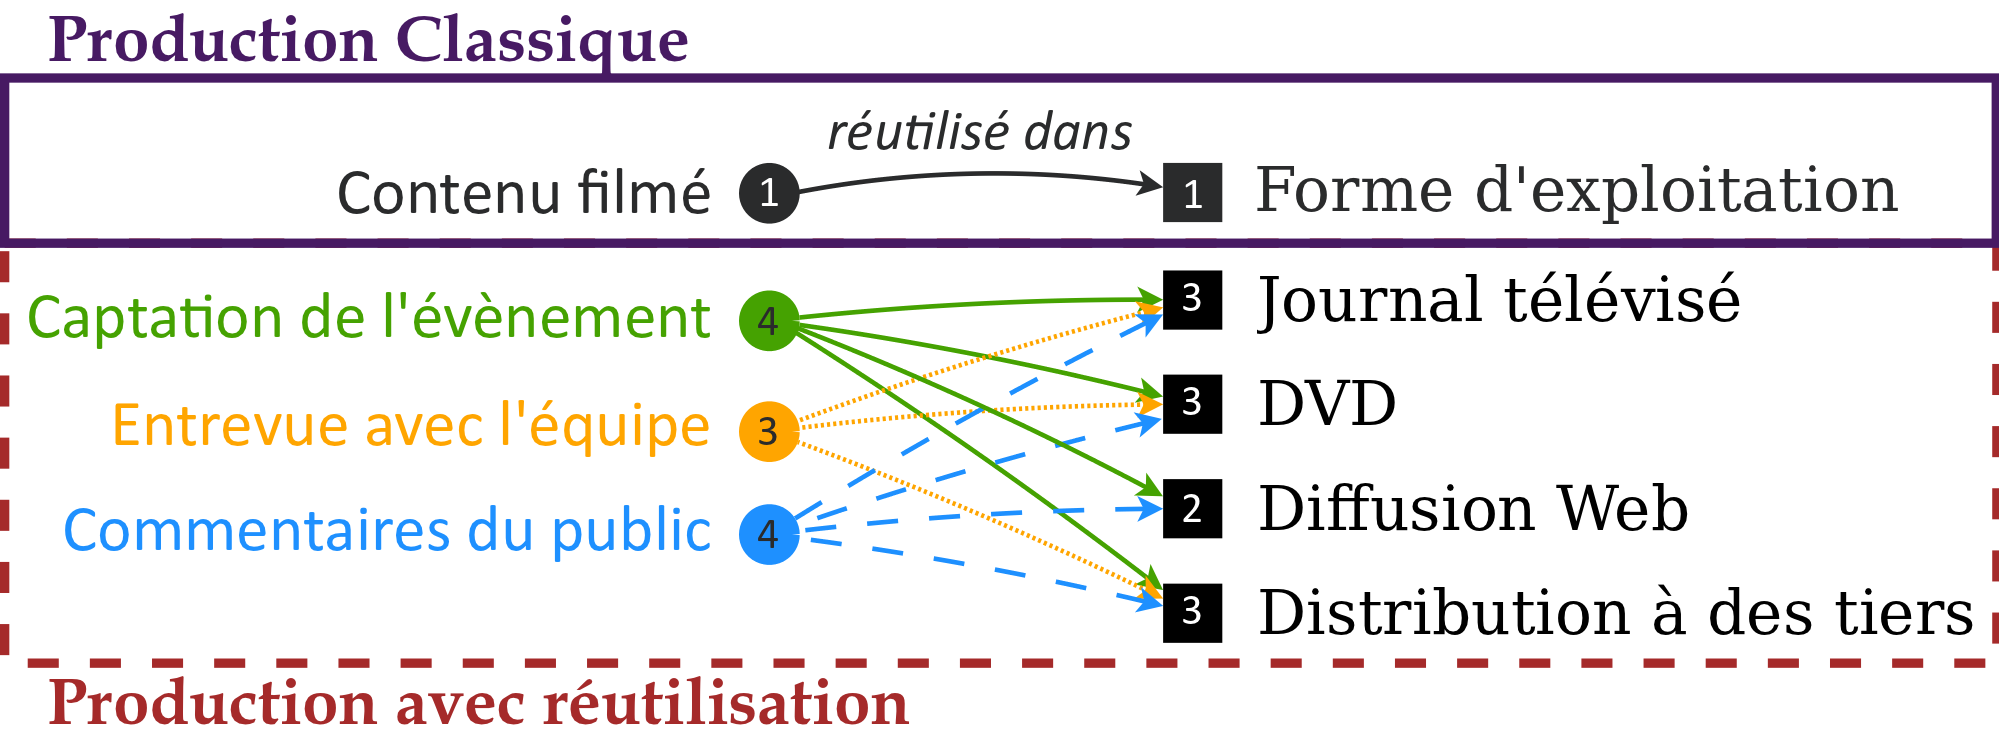
\includegraphics[width=0.7\textwidth]{images/UC-Tahnhauser-v1fr.png}
\caption{Modèle de la production classique comparé avec une production avec réutilisation}
\label{img:intro:reuse}
\end{figure}

Chaque cas de réutilisation tire sa matière première d'à peu près la même base de contenu filmé, mais en tire partie d'une manière propre à chaque forme d'exploitation visée. 
En effet, chaque audience a ses attentes, de même qu'il existe des contraintes techniques spécifiques pour chaque contexte d'exploitation. 
%En effet, il existe des contraintes techniques et des attentes spécifiques à chaque contexte d'exploitation. 

Ces spécificités exigent des variations dans la qualité de l'encodage, le format d'encapsulation utilisé, le montage réalisé, l'habillage du contenu etc. 
Par exemple, les contraintes de diffusion sur le Web implique d'encoder la vidéo dans un format spécifique et de multiples résolutions, généralement plus petites que pour la diffusion télévisée. 
Ensuite, le montage d'une bande-annonce possède un rythme généralement plus rapide que celui des bonus de DVD. 
Finalement, les cas d'exploitation gérés par la chaîne de télévision posséderont un habillage spécifique (logo de la chaîne, message d'annonces etc.) que ne partageront pas forcément les versions vendu à des organisations tierces. 

L'exemple des commentaires du public -- voir la Figure \ref{img:intro:reuse-process} -- permet de montrer à quels moments des transformations doivent être effectuées afin de produire les différentes formes d'exploitation :
\begin{liste} 
	\item[$\bullet$] On considère que deux commentaires de spectateur ont été tournés. 
	\item[$\bullet$] Un des commentaires est intégré au montage du journal télévisé, alors que les deux sont utilisés pour créer la bande-annonce. La bande-annonce est elle-même intégrée au montage du DVD. 
	\item[$\bullet$] Au moment de la finition, l'encodage de la bande-annonce est adapté à la qualité DVD et Web. De même, le journal télévisé est encodé à la fois pour une diffusion en définition standard (SD) et haute-définition (HD).
\end{liste}


\begin{figure}[ht!]
\centering
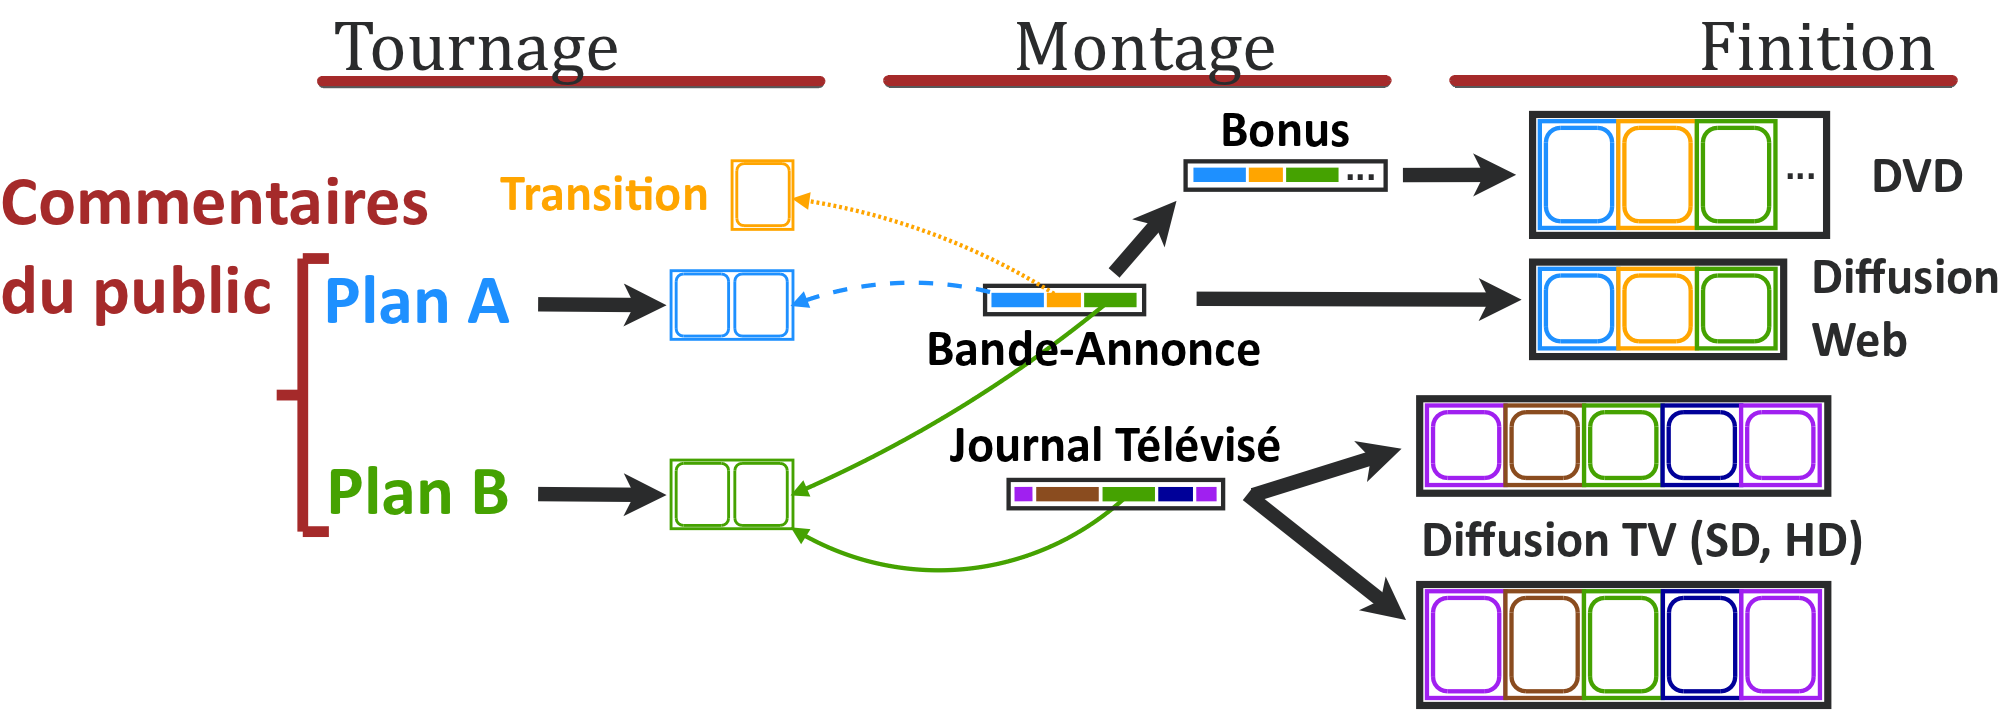
\includegraphics[width=0.8\textwidth]{images/EX-Content-Production-v7fr.png}
\caption{Étapes et transformations des contenus pour chaque forme d'exploitation des commentaires des spectateurs}
\label{img:intro:reuse-process}
\end{figure}

% Dans cet exemple, on distingue deux types d'opérations effectuées sur le contenu ; 
% la sélection de séquences au moment du montage qui correspond à une décision éditoriale (quel contenu va-t-on présenter à l'audience ?) ; 
% la tranformation de l'enregistrement du contenu qui correspond à des choix techniques (quelle méthode d'enregistrement va-t-on utiliser ?).
% Afin de préciser la nature de ces opérations, nous présentons différentes approches de la réutilisation des contenus.


\subsection{Besoins en modélisation (n)}
Le scénario d'usage que nous venons de voir présente un exemple de production incluant directement plusieurs formes d'exploitations pour des contenus produits en collaboration avec deux organisations professionelles et des amateurs. 
Ce scénario permet d'illustrer des opérations de transformation des contenus qui ne se limite pas à une réutilisation brut de matériel. 
On distingue ainsi plusieurs types de transformations qui définissent par les objets d'entrée et de sortie nos besoins de modélisations :
\begin{liste}
	\item le \e{transcodage} d'un contenu d'un format/encodage/résolution à l'autre afin de satisfaire aux contraintes techniques propre à un médium ou un canal de distribution. 
	Par exemple, le journal télévisé distribué dans 2 types de définitions ou bien la bande-annonce préparé pour une diffusion Web et DVD.
	%retraitement

	\item le \e{montage} différencié d'une séquence de contenu suivant la forme éditoriale dans laquelle elle s'insère.
	Le montage des commentaires du public sera plus rapide et dense pour la bande-annonce que pour le journal télévisé. 
	Ce dernier utilisera aussi moins de contenu pour rester sur les commentaires les plus construits ou marquants.
	%rééditorialisation 

	\item l'\e{intégration} d'une séquence montée dans de multiple formes d'exploitations. 
	Par exemple, la bande-annonce est un montage de plusieurs commentaires du public. 
	Elle sert, telle quelle, à la fois sur le site Web de la chaîne et dans les bonus du DVD. 
\end{liste}

De plus, si l'on reprend le scénario depuis la commande de tournage, on se rend compte qu'il existe de nombreux types d'informations que l'on peut collecter sur les objets audiovisuels construits :
\begin{liste}
	\item le genre de l'objet audiovisuel à construire qui détermine un schéma de \e{structure éditoriale}. 
	\item la commande de tournage qui fait office de \e{prescription} de la forme et du contenu de l'objet à produire.
	\item le tournage dont le résultat constitue la \e{réalisation} de la commande, c'est-à-dire le fichier vidéo créé.
	\item une fois le contenu produit, on peut en établir une \e{description} qui se révèlera plus ou moins proche de la prescription.
	\item le montage qui détermine la \e{composition} de l'objet audiovisuel.
	\item l'\e{organisation de la production} de manière générale, c'est-à-dire la division des tâches entre contributeurs. 
\end{liste}

Nos besoins en modélisations peuvent donc se résumer par les assertions suivantes : 
\begin{liste}
	\item[(B1)] rendre les objets et les fragments audiovisuels \g{autonomes} implique de les modéliser sur différents niveaux (technique, esthétique, éditorial etc.). 
	Chaque niveau de modélisation de ces objets correspond au résultat d'opérations effectuées durant le processus de production audiovisuel.
	Ainsi, chaque niveau peut être repris séparément de l'ensemble.

	\item[(B2)] rendre les objets et les fragments audiovisuels \g{réutilisables} implique de leur associer de multiples connaissances dès le début et tout au long de leur cycle de vie.
	Ces connaissances doivent correspondre à celles mobilisées par les contributeurs (humain ou logiciel) de la chaîne de production.
	Chaque type de connaissance s'associe à un niveau spécifique de l'objet audiovisuel de manière à faciliter leur recherche.

	% \item[(B3)] : 
\end{liste}

% À chaque niveau de modélisation des objets et fragments audiovisuels correspond des types de connaissances. 
On notera que la modélisation des objets et des connaissances associées s'enrichit suivant le déroulement de la chaîne de production.
\section{Qu'est-ce qu'un objet audiovisuel numérique ?}\label{sec:dav}
\e{
Dans le monde de l'audiovisuel, certaines notions implicites déterminent la manière dont les professionnels se représentent les objets qu'ils produisent, manipulent, échangent etc. 
L'objectif de cette section est d'expliciter les définitions de ces objets, d'en faire un inventaire (\ref{sec:pv-av}).
Notre démarche ne se limite cependant pas à la vision des professionnels de la production, puisque nous comparons leurs concepts avec ceux d'autres communautés, en vue d'identifier des écarts ou des manques que nous pourrons intégrer dans notre travail.
Ainsi, la communauté des bibliothèques numériques examine plus en détails les relations qui existent entre les résultats d'un processus de création (\ref{sec:pv-bn}). 
La communauté de l'ingénierie documentaire et des sciences de l'information et de la communication invoque quant-à-eux la notion de document, généralement fort absente dans la communauté audiovisuelle, et propose une vision plus fine des différents états de la fabrication et de la consultation d'un contenu audiovisuel (\ref{sec:pv-id}).
Ces deux perspectives apportent une richesse conceptuelle qui, au moment d'examiner les modélisations de l'audiovisuel existantes, nous permettra de mieux identifier ce qu'ils représentent et ne représentent pas.}



\subsection{Du point de vue de l'audiovisuel}\label{sec:pv-av}
Afin de clarifier la notion d'objet audiovisuel, nous présentons la manière dont les professionnels se représentent ses différents composants.
Nous reprenons une liste de définitions proposées par \cite[p.77]{Cox2006} (sauf pour la notion d'\pc{Asset} que nous empruntons à \cite{Austerberry2004}) que nous \ciel{traduisons} et commentons en français : 
\begin{liste}
	\item \pc{Work} (Oeuvre) : \ciel{un travail de création artistique produite ou construite par les efforts conjugués d'une personne ou d'un groupe}.
	Cette définition est clairement reprise du modèle FRBR (voir ci-après) et s'intègre d'ailleurs assez mal avec le reste de la modélisation.

	\item \pc{Essence} : \ciel{toute donnée (numérique) ou signal (analogique) nécessaire à la représentation d'une modalité d'expérience perceptive (visuel, olfactive, auditive etc.)}.

	\item \pc{Material} (Matériel) : \ciel{toute Essence ou combinaison d'Essences (image, son etc.)}. 
	Ainsi, on peut parler de matériel audiovisuel, qui est une combinaison d'Essence audio et visuelle.
	En résumé : Essence/Matériel sont ce que l'on transmet au spectateur, l'Essence se limitant à une modalité.

	\item \pc{Metadata} (Métadonnées) : \ciel{les données qui transportent des informations sur le Matériel -- par exemple des informations d'identification, codage des essences, timeline, propriété intellectuelle etc.}
	Matériel et Essence se différencient des Métadonnées par leur vocation : transmettre une expérience perceptive au spectateur ou transmettre des informations sur le Matériel.

	\item \pc{Content} (Contenu) : \ciel{le Matériel et les métadonnées associées}. 
	Il est particulièrement intéressant de noter l'écart entre cette définition ensembliste et le sens commun. 
	Ici, il s'agit de pouvoir désigner un objet à manipuler, ce qui a de la valeur en terme d'échange, mais non de référer à la signification de l'Oeuvre.
	En résumé : Contenu = Matériel + Métadonnées.

	\item \pc{Instance} : \ciel{une occurrence spécifique et unique de Matériel, Métadonnée ou Contenu}.
	Là encore, l'explicitation de la définition renvoit à un éléments appartenant à trois ensembles. 

	\item \pc{Asset} : \ciel{un asset est ce qui a de la valeur. Le contenu ne suffit pas forcément à représenter un asset. Le propriétaire du contenu doit avoir le droit d'utiliser le matériel avant de pouvoir l'appeler un asset.} 
	En résumé : Asset = Contenu + Droits.
\end{liste}

% On peut résumer ces définitions par l'équation suivante : Asset = Contenu(Matériel + Métadonnées) + Rights.
Cette liste de définition semble intégrer plusieurs manières de se représenter le travail de la production audiovisuelle et ses résultats :
\begin{liste} 

	\item[\g{artistique}] : le travail de création artistique qui aboutit au résultat abstrait d'une Oeuvre. 
	C'est cette réalisation abstraite qui est protégée par la propriété intellectuelle et peut faire l'objet d'une cession de droits.
	Pourtant, la relation entre l'Oeuvre et l'Asset n'est pas établie clairement.

	\item[\g{concrète}] : plusieurs définitions font référence aux résultats concrets de la production (les Instances de Matériel, de Métadonnée et donc de Contenu, les Essences).

	\item[\g{commerciale}] : la notion d'Asset aborde le résultat du travail de production sous l'angle de l'exploitation commerciale. 
	Si on prend l'exemple de la diffusion d'un Contenu qui n'appartient pas à la chaîne, cette diffusion ne peut se faire qu'après achat des droits qui établissent en détails les conditions d'exploitation cédées (zone géographique de diffusion, nombre de rediffusion, limite dans le temps etc.).
	
\end{liste}

% Définition de Media Asset etc. de \cite{Furht2008}.


\subsection{Du point de vue des bibliothèques numériques}\label{sec:pv-bn}
Le \e{Functional Requirements for Bibliographic Records : object-oriented} (FRBRoo) est un modèle conceptuel développé par \cite{Aalberg2008}.
Il vise à faciliter l’échange d’information entre les bibliothèques numériques et les musées. 
Il permet de représenter les personnes participant aux différentes étapes de construction d’un objet culturel, depuis l’idée jusqu’à la réalisation matérielle.

La particularité de cette modélisation est de disséquer les objets culturels dans le but de leur conservation.
Ainsi, le modèle cherche à établir quelles sont les liens généalogiques entre les objets conservés, déterminer les inspirations, les adaptations etc. afin de mettre en évidence des relations culturelles.
Ce souci du détail clarifie les relations entre les objets et par conséquence le processus de création. 
Chaque objet culturel possède trois niveaux de modélisation qui sont présentés dans leur ordre chronologique d'apparition dans le processus de création :
\begin{liste}
	\item le niveau des \e{idées} ou des \e{oeuvres} (\pc{Work}) n’ayant pas pris corps dans une matérialité externe à un sujet (par exemple une mélodie ou une histoire qui nous reste dans la tête). 

	\item le niveau des \e{formes d'expression} (\pc{Expression}) où l'on distingue parmi toutes les formes possibles pour exprimer une idée (une nouvelle écrite, ses traductions, une adaptation de nouvelle en scénario, une lecture de cette nouvelle etc.).
	On se situe à un niveau intermédiaire qui définit des formes abstraites de  réalisation.
	Il faut préciser qu'on parle de forme abstraite dans le sens où il n'existe pas de réalisation concrète, ce qui n'empêche pas de les définir précisement et donc de distinguer de multiples variantes d'expressions :

	\ciel{
	the form of expression is an inherent characteristic of the expression, any change in form (e.g., from alpha-numeric notation to spoken word, a poem created in capitals and rendered in lower case) is a new expression. Similarly, changes in the intellectual conventions or instruments that are employed to express a work (e.g., translation from one language to another) result in the creation of a new expression.} (\cite{Aalberg2008})
	
	\item le niveau des \e{réalisations concrètes} comme les porteurs physiques d’information (\pc{Information Carrier}) portant les expressions (livre, partition, cd-rom etc.). 
	À ce niveau, il faut également distinguer entre l’original (\pc{Manifestation Singleton}) et les copies manufacturées (\pc{Item}) issues d’un modèle de publication (\pc{Manifestation Product Type}). % à rapprocher de la notion de Media Profile dans MPEG-7
\end{liste}

\paragraph{Discussion et comparaison}
Dans la perspective audiovisuelle présentée précédemment, la relation entre Oeuvre et Asset est bien plus floue.
À la fin du processus de création, il apparaît évident que l'on a produit un Asset, mais la notion d'Oeuvre, et donc de l'idée qui a amené à la création, échappe aux systèmes de gestions d'objets audiovisuels.
Ces systèmes ne sont pas fait pour gérer la propriété intellectuelle, ou bien rendre compte des adaptations d'une même idée en plusieurs réalisations.

Par ailleurs, on peut identifier des correspondances entre les notions de FRBR et celles du monde de l'audiovisuel :
\begin{liste}
	\item un \pc{Manifestation Singleton} correspond à la réalisation concrète originale du processus de production, ce qui correspond à la notion de \e{master} dans l'audiovisuel.
	
	\item dans le cadre du numérique, la notion de \pc{Manifestation Product Type} existe dans les cas des documents structurés associés à des feuilles de style.
	On peut noter, que cette notion se rapproche de celle de \pc{MediaProfile} définie dans MPEG-7 à la section \ref{sec:mpeg7}.

	\item un \pc{Item} correspond à une \pc{Instance} de \pc{Contenu} ou de \pc{Matériel}.
	\item un \pc{Information Carrier} correspond à un \e{medium} (media en anglais).

	\item une \pc{Expression} correspond à la notion de \e{format} en audiovisuel.
	Cette notion est centrale puisqu'elle détermine la manière dont la production se déroulera, les moyens attribués, s'il s'agit de l'adapation d'une Oeuvre pré-existante, il faut d'abord vérifier si l'on dispose des droits etc.
	Cette notion est représentée comme une propriété d'un \pc{Contenu} dans ses Métadonnées mais ne permet pas de rendre compte de la relation entre Oeuvre et format d'expression.
\end{liste}





\subsection{Du point de vue de l'ingénierie documentaire}\label{sec:pv-id}
Nous examinons principalement la lignée des travaux de recherche menés initiallement par \cite{Bachimont1998}, formalisés comme une théorie du support numérique dans \cite{bachimont:hdr} puis affinés dans \cite{bachimont:icc}. 
% De nombreux travaux ont repris ce positionnement pour 
Ce positionnement a été approfondi dans le domaine de l'audiovisuel par d'autres auteurs dont \cite{Prie1999}, \cite{Troncy2004}, \cite{Morizet-mahoudeaux2005a}, \cite{Gaillard2008}.

\subsubsection{Les dimensions de l'inscription matérielle}
Ces travaux reposent sur les concepts d'\pc{Inscription}, de \pc{Conte\-nu} et de \pc{Support}. 
La définition d'un \pc{Contenu} permet de relier ces concepts : 
\ciel{
	Un contenu est une forme inscrite sur un support se prêtant à une interprétation à travers laquelle elle fait sens pour quelqu'un ou une communauté.
	C'est donc une \e{forme matérielle interprétable.}} \parcite{bachimont:icc}

Un point à noter est que le contenu est bien une inscription matérielle, non pas le sens que l'on aurait construit de son interprétation.
En tant qu'inscription matérielle, \citeauthor{bachimont:icc} distingue trois dimensions qui caractérisent la manière dont un contenu exprimé sera enregistré, puis restitué.
Dans chacune de ces dimensions (expression, conservation, restitution) intervient une forme, un support et un dispositif, voir la Figure \ref{img:inscriptions}.
Le dispositif a pour objectif de transformer une forme A inscrite sur un support $\alpha$ en une forme B inscrite sur un support $\beta$.

\begin{figure}[ht!]
\centering
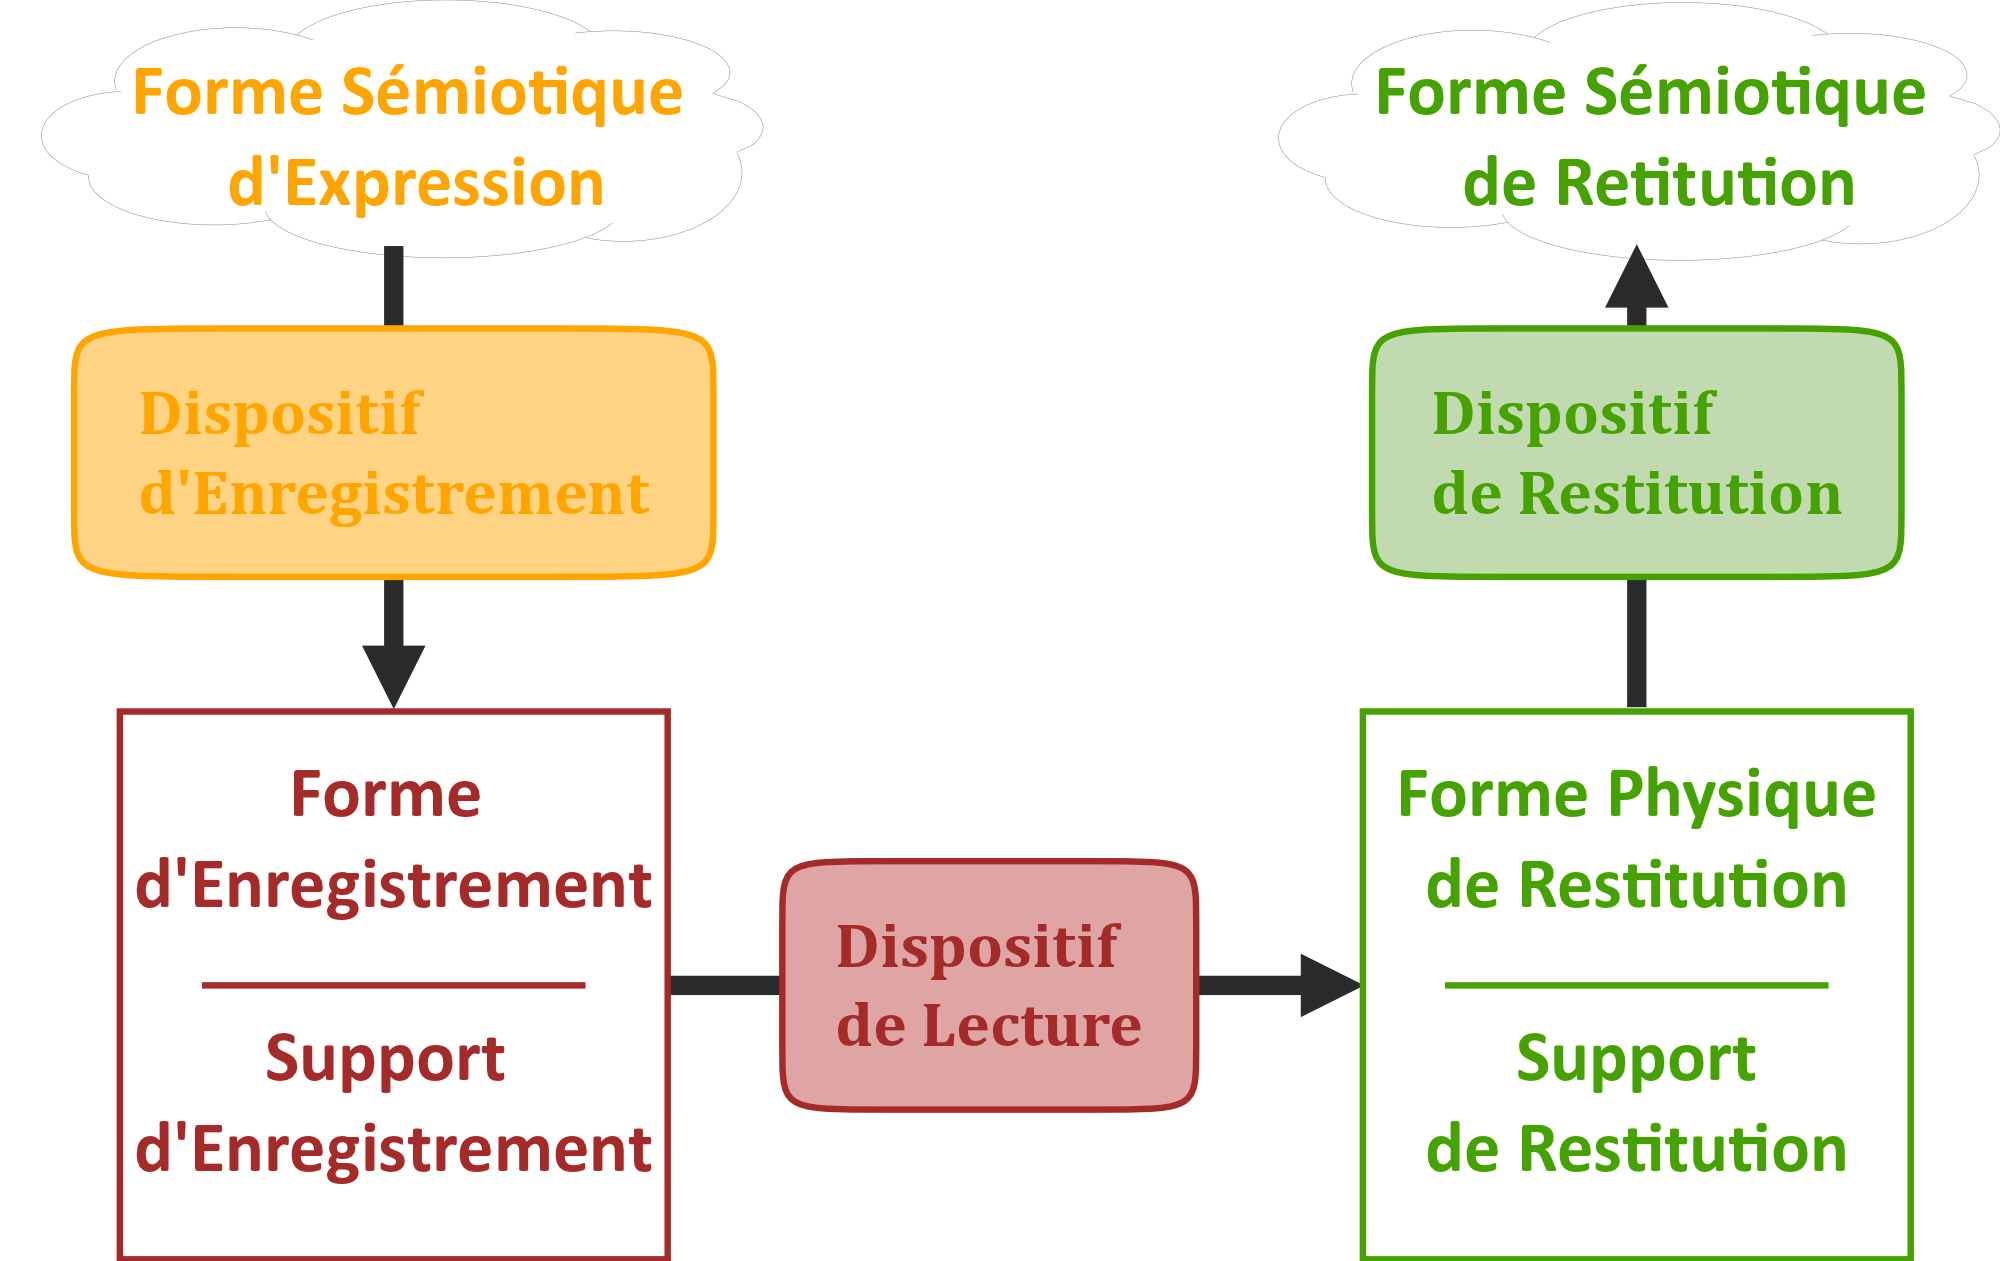
\includegraphics[width=0.7\textwidth]{images/DimensionsInscriptions-v2.png}
\caption{Les dimensions de l'inscription matérielle : forme, support et dispositif}
\label{img:inscriptions}
\end{figure}


\begin{listeni}
	\item \g{dimension de l'expression}
	\begin{liste}
		\item \e{forme sémiotique d'expression} (FSE) : Il ne s'agit pas simplement d'une forme à inscrire, mais bien d'un contenu, puisque l'auteur exprime une intention selon un code sémiotique qui permet à d'autres de l'interpréter.
		La forme sémiotique d'expression est considéré comme volatile et non-permanente, comme la parole ou bien une mélodie sifflée.

		\item \e{dispositif d'enregistrement} (DE) : le dispositif matériel qui réalise l'inscription de la forme d'expression sur un support afin d'assurer sa conservation.
		Cette inscription consiste en une sélection et une configuration de la forme d'expression en une forme d'enregistrement, comme le réalise par exemple un microphone ou bien une caméra.
	\end{liste}

	\item \g{dimension de la conservation}
	\begin{liste}
		\item \e{forme d'enregistrement} (FE) : une forme d'inscription qui assure l'enregistrement, c'est-à-dire la persistance matérielle du contenu sur un support. 
		Par exemple, le code binaire pour un support numérique, un signal mesuré sur une échelle physique quelconque pour l'analogique (magnétique, tension électrique etc.), les lettres de l'alphabet pour l'écriture etc.

		\item \e{support d'enregistrement} (SE) : l'objet matériel sur lequel on inscrit une forme pour conserver et préserver le contenu.
		Par exemple, le papier pour un texte, un 45 tours pour la musique, une mémoire magnétique (disque dur etc.) ou optique (CD etc.) pour le numérique, une cassette vidéo pour une vidéo analogique etc.

		\item \e{dispositif de lecture} (DL) : le dispositif matériel qui réalise la transformation de la forme d'enregistrement en une forme physique de restitution.
		Par exemple, un tourne-disque pour les 45 tours, un ordinateur avec un lecteur multimédia pour une vidéo numérique, un magnétoscope pour une cassette vidéo etc.
	\end{liste}

	\item \g{dimension de la restitution}
	\begin{liste}
		\item \e{forme physique de restitution} (FPR) : une forme sous laquelle l'inscription est présentée pour être perceptible.
		Par exemple, des pixels de couleurs pour une vidéo, une onde sonore pour une musique etc.
		Les normes MPEG-1 et MPEG-2 définissent des techniques d'encodageet de compression d'images et de vidéos.
		Il s'agit donc de normes qui permettent la numérisation de la FPR.
		
		\item \e{support de restitution} (SR) : il s'agit de l'objet matériel sur lequel la restitution du contenu s'inscrit, ce qui permet à un lecteur d'appréhender un contenu par ses sens. 
		Par exemple, un écran pour un signal visuel ou bien l'air ambiant pour le son.
		Cet élément est relié au dispositif de lecture, qui se contente de fournir une forme sans la rendre perceptible à son lecteur, ainsi qu'au dispositif de restitution, qui lui permet au lecteur de l'interpréter.
		
		\item \e{dispositif de restitution} (DR) : le dispositif matériel qui permet de transformer une forme physique en une forme sémiotique.
		Il peut s'agir d'un téléviseur ou d'un écran d'ordinateur pour une forme visuelle, de haut-parleurs pour une forme sonore.
		
		\item \e{forme sémiotique de restitution} (FSR) : une forme de représentation intelligible par l'utilisateur qui en connaît les codes sémiotiques.
		Les formes sémiotiques usuelles sont l'image, la musique, le bruit, la parole etc.
	\end{liste}
\end{listeni}

L'intérêt de cette définition du contenu par état (forme/support) est également de pouvoir introduire la notion de document et de formes documentaires, complètement absente des deux premières perspectives que nous avons examinées.


\subsubsection{Le document audiovisuel numérique}\label{sec:docnum}
\cite{Morizet-mahoudeaux2005a} définissent un document comme un contenu qui peut servir de référence par sa consistance matérielle dans le temps : \ciel{a document is a \e{content} instituted by a \e{publication act}, written down a medium, which possesses a \e{spatial} and \e{temporal delimitation}}.

\begin{liste}
	\item \e{permanence dans le temps} : \ciel{la consistance des signes matériels qu’il porte doit être assurée quelque soit le moment de leur consultation.} \parcite{Bottini2010}

	\item \e{délimitation spatiale} : un document se définit par ce qu'il contient et ce qu'il ne contient pas.
	C'est par ses frontières que le document ouvre la possibilité de sa lecture et de son interprétation.

	\item \e{délimitation temporelle} : la naissance d'un document est institué par un acte de publication, c'est-à-dire le moment où l'on arrête de faire varier sa forme matérielle, pour le faire rentrer dans une sphère médiatique.

	\item \e{intentionnalité} : le document est porteur d'une signification qui ne se résume pas à sa forme matérielle.
	On peut distinguer les documents possédant une intentionnalité \e{a priori} (l'objet matériel a été créé pour porter une intentionnalité documentaire) et ceux dont on attribue une intentionnalité \e{a posteriori} (par exemple, des outils de chasse retrouvés par un archéologue qui les interprètent pour reconstruire les habitudes de l'époque).
\end{liste}


Pour \cite{Leleu-Merviel2004}, le document comporte à la fois une dimension \e{sémiotique} qui renvoit au contenu (signes et sens), \e{technique} qui renvoit aux données (format d'enregistrement, codage et transmission de signaux) et \e{médiatique} qui renvoit à des processus de socialisation, de diffusion, de réception et de consultation.
\cite{Leleu-Merviel2005} décrit cette dernière dimension comme étant la dimension d'accès aux données, un accès qui peut être organisé spatialement et temporellement :
\begin{liste}
	\item la \e{scénique} est la manière de transposer des données en une réalité concrète : \ciel{la forme visuelle et sonore de l’inscription spatiale des fragments}. %FPR+SR
	\item la \e{scénation} est la manière de restituer temporellement à l'utilisateur les fragments d'un document : \ciel{la structure organisée d’événements et/ou d’états avec lesquels l’utilisateur est effectivement mis en interaction}. %DR+FSR
\end{liste}

On retrouve dans cette définition, la caractérisation de l'inscription matérielle faite par \cite{bachimont:icc} avec les correspondances suivantes : 
\begin{liste}
	\item les données correspondent aux éléments matériels qui vont de la FE (l'enregistrement en binaire, inaccessible et illisible pour l'humain) jusqu'à la FPR (qui rend perceptible le contenu). 
	\item la dimension sémiotique renvoit à la FSR ainsi qu'à ses structuration, mais aussi à la configuration par le DR de son accès dans ses dimensions spatiale (scénique) et temporelle (scénation).
	% \begin{liste}
	% 	\item la scénique renvoit à l'association FPR + SR qui rend perceptible le contenu.
	% 	\item la scénation renvoit à l'association FSR + DR qui conditionne l'interprétation du contenu.
	% \end{liste}
\end{liste}

Cette définition développe celle proposée antérieurement par le réseau thématique pluridisciplinaire 33 (RTP-DOC, \cite{Pedauque2003}) qui fait référence dans les communautés scientifiques engagées dans les questions documentaires.
Leur définition du document comporte trois dimensions similaires : le document comme \e{forme} (la dimension matérielle dans laquelle s’incarne le contenu et qui permet sa manipulation), le document comme \e{signe} (il est porteur d’un sens intentionnel), et le document comme \e{médium} (sa dimension sociale, d'échange et de communication).

\paragraph{Le document audiovisuel}
Dans le cas de l'audiovisuel, la forme sémiotique qui est inscrite sur le support d'enregistrement est temporelle, non-interactive et multi-modale.
En effet, les images et le son se présentent au lecteur de manière successive, selon un ordre, un rythme et une durée pré-définis.
La forme audiovisuelle se constitue de la superposition de ces flux visuels et sonores \parcite{Prie1999}.
Or un enregistrement se fait nécessairement sur un espace matériel, ce qui implique de se donner un moyen de représenter spatialement le temps, et d'y associer ces images et ces sons.
L'utilisation de code temporel (\e{timecode}) permet de marquer l'écoulement du temps et de réaliser cette synchronisation des flux.
Une fois cette synchronisation faite, les flux peuvent être lu ensemble pour recréer le flux audiovisuel.
Mais il devient également possible de représenter graphiquement ces flux afin de les appréhender de manière synoptique, quoique imprécise, pour faciliter sa manipulation et son analyse\footnote{Nous mentionnons en particulier le logiciel \gui{Ligne de Temps} développé par l'Institut Recherche et Innovation du Centre Pompidou. Voir \url{http://iri-web.centrepompidou.fr/outils/lignes-de-temps/} pour plus de détails sur son fonctionnement.}. 
En effet, on peut représenter une successsion d'images en sélectionnant à intervalle régulier l'un d'entre elles, pour autant on ne peut réduire l'interprétation d'un objet audiovisuel à cela.
La représentation graphique du son par sa fréquence est bien plus problématique, puisqu'elle ne permet pas de distinguer les moments de paroles et de musique, ni les mots prononcés etc.


 % doc adaptatif
 % doc av
 \subsubsection{Personnalisation et adaptation}
La particularité du document numérique par rapport au document papier, est la coupure entre le support d'enregistrement et le support de restitution. 
Ainsi, l'enregistrement des données ne suffit pas à rendre le document lisible, il faut pour cela la médiation des dispositifs de lecture et de restitution, qui par calcul, reconstruisent le document au lecteur.
Cette reconstruction peut alors faire l'objet d'une configuration prenant en compte la situation de lecture (lecteur, contexte de travail, dispositif matériel etc.), pour proposer non pas une vue canonique du document, mais une vue personnalisée ou adaptée à cette situation.
Ces questions sont traités dans les domaines des hypermédia adaptatifs \parcite{Balpe1990}, de la modélisation utilisateur et des documents virtuels personnalisables \parcite{Leleu-Merviel2004}. \cite{Iksal2002} a réalisé une étude approfondie de ces questions et \cite{Garlatti2004} détaillent leur fonctionnement dans le cadre du projet d'un Web sémantique.

Le fait de nommer les documents ainsi construits de \e{virtuel} renvoit également au caractère dynamique de cette construction, qui s'oppose à la matérialité du document traditionnel, à sa \e{permanence}, son statut de \e{référence} destinée à être \e{partagée} par plusieurs lecteurs \cite[pp.185-186]{bachimont:icc}. 
Ainsi, l'adaptation du document construit des vues perceptibles et manipulables dans l'ici et le maintenant de l'interaction entre le lecteur et les dispositifs de lecture qu'on lui fournit.
Les documents deviennent alors des ressources dont un système se saisit pour composer de nouveaux points de vue, rendu plus pertinent par leur adaptation au contexte de lecture :

\ciel{
conserver, retrouver l’information n’est pas suffisant. 
Pour qu’elle puisse être utile, il faut qu’elle puisse être exploitée, c’est-à-dire traitée et rapprochée d’autres de façon à produire de l’information nouvelle. 
Produire du sens n’est, pour l’essentiel, que rapprocher des informations disparates jamais rassemblées auparavant.} \parcite{Balpe1990}


On remarque que deux types de systèmes d'adaptation se distinguent \parcite{DeBra1999} : 
\begin{liste}
	\item les systèmes \g{adaptables} qui fonctionnent à partir d'une requête de l'utilisateur (quelque soit la forme de celle-ci, formulaire, questionnaire etc.) et des informations sur l'utilisateur (connaissances et préférences).
	Dans ce cadre, l'utilisation d'une modèle de l'utilisateur est primordiale pour mener à bien l'adaptation.
	\item les systèmes \g{adaptatifs} qui repose sur l'observation de l'utilisateur pour déduire ses connaissances et préférences. 
	De la sorte, le système déduit les informations sur l'utilisateur, plutôt qu'il ne le consulte (comme dans la première approche).
\end{liste}

Dans le cadre du projet MediaMap, il est prévu qu'un système \e{adaptable} soit développé pour faciliter la prise de vue par des contributeurs amateurs.
Notre modèle doit ainsi permettre l'adaptation de scripts de tournage, ce qui implique de représenter d'une part les contributeurs et leurs connaissances, le vocabulaire du script et la structure du document audiovisuel.
Toutefois, la manière de réaliser l'adaptation n'est pas traitée dans notre modèle, mais laissée aux développeurs d'applications.
L'objectif de notre modélisation étant de fournir des éléments de contexte pour faciliter les échanges de connaissances le long de la chaîne de production.

% \ciel{
% Cependant en numérique, les fragments existaient, au moins potentiellement, dans la mémoire de la machine, ce n’est que leur actualisation sur l’écran et la forme qu’elle prend qui se construit dans l’ici et maintenant de l’interaction. 
% Celle-ci est donc nécessairement volatile. De plus, elle change à chaque fois.
% Ainsi c’est l’affichage, [\dots] qui varie, mais non le document lui-même tel qu’il est mémorisé au niveau des données.}

% \ciel{
% conserver, retrouver l’information n’est pas suffisant. 
% Pour qu’elle puisse être utile, il faut qu’elle puisse être exploitée, c’est-à-dire traitée et rapprochée d’autres de façon à produire de l’information nouvelle. 
% Produire du sens n’est, pour l’essentiel, que rapprocher des informations disparates jamais rassemblées auparavant.} (\cite{Balpe1990})

% % Deux pistes proposées par SLM : 
% Il est alors possible de construire des assemblage cohérent de fragments le temps d'une consultation (d'un affichage) par un utilisateur (documents virtuels personnalisables).
% Plus on a de connaissance sur son activité, ses tâches, ses compétences propres, plus il est alors possible de rendre cette assemblage pertinent. 

% Il est aussi possible de mettre à profit la description des documents pour construire des notions de voisinage indépendamment du profilage des utilisateurs. 
% La proximité entre deux documents pourra s'évaluer d'autant de manière qu'il y a de critères descriptifs.
% Ainsi, des informations auparavant éparpillées dans des documents papier différents pourraient être regroupés pour former de nouveaux assemblages

\subsubsection{Unité de contenu et structures documentaires}\label{sec:uc-sd}
La distinction entre \e{forme physique de restitution} (FPR) et \e{forme sémiotique de restitution} (FSR) sera essentielle pour l'examen des modélisations de l'audiovisuel.
Un changement de la FSR impacte la signification du contenu, alors que les changements sur la FPR ont une conséquence sur le plan perceptif, mais pas forcément sur la signification (un pixel mort ne change pas le sens d'une image).
Comme nous le verrons plus tard (\ref{sec:codesc}), beaucoup de modèles se focalisent sur la FPR, c'est-à-dire sur la caractérisation du signal par des descripteurs de bas-niveau que l'on pourrait qualifier d'objectif (texture, couleur, forme etc.).

La modélisation de la FSR se fonde sur une interprétation de la forme matérielle du contenu pour dégager ce que \cite{Prie2000} appelle des \e{structures documentaires}.
Une structure documentaire découpe le contenu en unités suivant une grammaire de (dé)composition.
\citeauthor{Prie2000} considère ainsi que \ciel{toute structure est sémantique et fait partie d'une structure d’indexation conceptuelle} qui renvoit donc à une utilisation \ciel{dans le cadre d'une tâche qui peut être une tâche de présentation}.
L'indexation conceptuelle est définie commme \ciel{explicitation de structures et de concepts contenus dans les documents numériques ou qui leur sont associés, pour mieux les exploiter}.
On construira donc des structures différentes suivant l'exploitation du contenu visée, qu'il s'agisse de produire une interprétation pour faciliter l'accès au contenu, de manipuler le contenu ou bien d'en fournir une présentation. 

\citeauthor{Prie2000} distingue ainsi le cas particulier de l'écriture.
Il s'agit d'une tâche à part où \ciel{l’intentionnalité de l’auteur se retrouve plus ou moins dans les structures documentaires} qu'il définit. 
Ces structures expriment des \ciel{connaissances \e{auctoriales} premières}, dans le sens où elles constituent le document et permettent sa médiatisation auprès d'un lectorat.
Cette structure documentaire première renvoit également à un genre documentaire, où elle puise une \ciel{une structure de présentation \e{canonique}}, souvent appelée structure logique par d'autres auteurs.
La notion de genre, amène à la notion de tradition de lecture, dont les éléments de structure canoniques prescrivent une interprétation du document.
Les auteurs peuvent ainsi identifier des communautés de lecteurs par les genres documentaires qu'elles mobilisent dans leurs activités.

La structure première ou canonique définit par l'auteur sert ensuite à d'autres communautés pour établir leur propre structure documentaires en fonction de leurs usages.
Lorsque plusieurs structures sont associées à un document, \cite{Abascal2003} et \cite{Abascal2004} parlent alors de documents \ciel{multistructurés}, chacune répondant aux contraintes d'un usage.

La multiplicité des structures documentaires n'éclaire pas pour autant sur leur nature.
\cite[p.191-192]{bachimont:icc} propose ainsi de distinguer entre quatre niveaux :
\begin{liste}
 	\item \e{niveau physique} : le document est avant tout un assemblage de formes matérielles (unités de contenu), organisées et destinées à faire sens pour un lecteur.

 	\item \e{niveau de typage du contenu} : chaque unité de contenu possède un type qui détermine sa sémantique et les manipulations qu'il peut subir.
 
 	\item \e{niveau syntaxique} : des règles syntaxiques (grammaire) tirent parti du typage des unités de contenu pour régir leur organisation au niveau physique. 

 	\item \e{niveau conceptuel} : le typage d'une unité de contenu lui associe également une signification conceptuelle, indépendante des règles syntaxiques (comme \citeauthor{Prie2000} le fait remarquer avec les structures documentaires).
\end{liste}


La caractérisation de ces différents niveaux nous renvoit aux besoins de modélisations exprimés en \ref{sec:bm-av} (\g{B1 : autonomie} et \g{B2 : réutilisabilité}).

% on propose une modélisation logique du document qui repose sur la vision des contributeurs à sa production.


% paragraph{Discussion et comparaison}

 . 


\newpage
\section{Circulation et réutilisation des objets audiovisuels}\label{sec:gest}

% [Voir MXF, voir AAF ? \cite{Cox2006}
% [Identifiant : hors du cadre de la thèse, dépendant des choix applicatifs des organisations qui utilisent notre modèle. Plusieurs solutions peuvent être implementés via OWL, les URI pouvant être transformé.]

\e{
Si la promesse du numérique de faciliter la manipulation et la circulation des fichiers semble bien s'être réalisée, il n'est pas si évident de l'articuler avec les besoins de la production audiovisuelle (\ref{sec:besoins}).
Ce que l'on nomme la réutilisation des objets audiovisuels recouvre en réalité diverses pratiques et qui repose plus sur la notion d'objet métier ou d'objet numérique que sur la notion informatique de fichier.
Ainsi, la production souhaite récupérer des contenus existants ou produits par d'autres pour les intégrer dans sa propre chaîne de production, ou bien de réutiliser des contenus dans de nouveaux cadres d'exploitations (variation des modes de consommation, de distribution, de public etc.) quelque soit la manière dont l'informatique représente ces objets.}

\e{
Ces opérations qui semblaient a priori plus simple dans un environnement numérique sont en fait plus compliquées qu'il n'y paraît. 
Le numérique impose le calcul et l'explicitation des informations.
Or toutes les informations construites durant la chaîne de production ne sont pas encore intégrées dans les systèmes informatiques actuels.
Lorsque ces informations s'échangent sur papier, à l'oral, par mail ou dans des fichiers non-structurés, le lien avec les objets audiovisuels est alors bien souvent rompu, ce qui entraîne une limitation des traitements réalisables sur ces objets.}

\e{
Dès lors que l'on s'applique à structurer et associer ces informations aux objets audiovisuels, on ouvre la possibilité de récupérer, manipuler, transformer ces objets de nouvelles manières. 
Ainsi augmentés d'un supplément de contexte, les objets gagnent un supplément de manipulabilité susceptible de satisfaire aux besoins de la production audiovisuelle.
Une des solutions développée et utilisée dans l'industrie de la production audiovisuelle est le format conteneur qui encapsule divers types de données en un seul fichier. 
Ainsi, ces formats permettent d'associer de multiples types de fichiers multimédia avec d'autres types d'informations.}

\e{
Cette section a d'abord un souci de clarification des usages et des solutions adoptées. Nous nous intéresserons d'abord aux pratiques de réutilisations (\ref{sec:reuse}), puis nous expliquerons leurs impacts sur la chaîne de production audiovisuelle (\ref{sec:rechaine}). 
Enfin, nous présenterons des formats conteneurs qui assurent le transport des contenus et des informations associées le long de la chaîne de production (\ref{sec:wrapper}).}





%%%%%%%%%%%%%%%%%%%%%%%%%%%%%%%%%%%%%%%%%%%%%%%
\subsection{Caractériser la réutilisation}\label{sec:reuse}
% \subsubsection{Caractérisations de la réutilisation}\label{sec:caracs-reuse}
Nous avons vu grâce à l'exemple de la section \ref{sec:ex-reuse} à quel moment et dans quel type d'opérations la réutilisation pouvait se concrétiser. 
Nous proposons maintenant d'examiner la manière dont différentes communautés scientifiques  abordent la notion de réutilisation. 
Il s'agit de clarifier les hypothèses et les techniques proposées par chacune de ces communautés, et ainsi identifier les éléments pris en compte dans leur représentation du monde.  % Correction ?

\paragraph{Multimédia et Signal}
Prenons d'abord le cas de la communauté multimédia très orientée analyse et traitement du signal. 
Dans ce cadre, les constats mis en avant sont largement les mêmes que ceux que nous avons présentés précédemment (voir section \ref{sec:motiv}, multiplication et diversification des terminaux de lecture et des réseaux de communication, transformation des usages) :
 
\ciel{ 
Hundreds of device profiles are available for accessing online content and more announced everyday. These devices are connected through a wide variety of networks [\dots] As before, the issue of usage scenarios --activity type, user age and gender, time available, and prior knowledge of the subject matter-- continues to exist.} (\cite{Singh2004}).

Un point diffère cependant, le \gui{problème} de la variabilité des usages est considéré comme de même nature que la variabilité des technologies pour transférer et lire le contenu. 
En effet, l'approche de la réutilisation privilégiée par cette communauté consiste en une transformation automatique du contenu en fonction des paramètres d'un scénario de distribution et de lecture : 

\ciel{
Fundamental to this approach is the need to maintain a single copy of the content in its original form and to repurpose the content to fit the desired scenario in real time and in an automated fashion. [\dots] the next step in the repurposing process is to describe the content so that it can be understood and processed to fit delivery requirements --whether they're technical or usage based.} (\cite{Singh2004}).

L'approche automatique est justifiée par la difficulté à maintenir et gérer différentes versions d'un même contenu, en plus d'être coûteux et chronophage.
Ainsi, la décision humaine est simplement reportée au niveau du paramétrage du système de supervisation des opérations techniques.\\


\paragraph{Ingénierie Documentaire}
Dans la communauté de l'ingénierie documentaire, le principe est de pouvoir modéliser distinctement le message que l'auteur souhaite transmettre et la forme dans laquelle ce message se donne à voir par un lecteur. 
Cette tradition, que l'on pourrait faire remonter à la fin des années 60 avec la création du \e{Generalized Markup Language} (\cite{Goldfarb}) ancêtre des SGML, HTML, XML et consorts, repose sur le balisage d'un contenu source. 
Il s'agit alors d'identifier des fragments de contenu ainsi que leur structuration pour mieux les manipuler, quelque soit les opérations effectuées sur ces fragments (transformation, indexation, réécriture etc. \cite[chap.5.2]{Bachimont2004}). 
Les langages de modélisation documentaires tels que \e{Document Type Definition} ou \e{XML Schema} (\cite{Fallside2004}) permettent de contrôler par une grammaire les systèmes de balises construits en vue de formaliser des usages documentaires. 

Nous noterons le développement récent des \gui{chaînes éditoriales}, ces systèmes qui opérationnalisent l'hypothèse de base de l'ingénierie documentaire reformulée par \cite{Crozat2004} de la sorte : \ciel{tout contenu numérique consiste en une ressource qu’un calcul permet de publier dynamiquement sous différentes formes contextualisées}. 

Ces systèmes se concentrent ainsi sur le maintien d'une ressource de base que l'on peut transformer ensuite de diverses manières, soit par une transformation technique que l'on pourra automatisée, soit par une transformation manuelle réglée sur les usages visés (\cite{Crozat2011}) : 
\begin{liste}
	\item le polymorphisme \ciel{consiste en la possibilité technique de disposer d'une source unique de contenu et de la transformer à volonté selon les supports et mises en formes désirés}. Dans ce cas, on établit une séparation entre le fond (la source documentaire) et les formes de publication qui permet de mettre en place une production multi-support.

	\item la réutilisation \ciel{par référence (sans duplication d'information) consiste en la possibilité technique de désassembler et de ré-assembler des fragments de contenu afin de les partager entre plusieurs documents}. Dans ce cas, l'opération repose sur une modélisation séparée du scénario (la structuration) et le contenu.

	\item la ré-éditorialisation est une \ciel{remise en contexte de fragments issus d'un fonds documentaire, par leur ré-agencement au sein d'un nouveau document, leur augmentation par une création de contenus spécifiques et leur publication sur un nouveau support et/ou pour un nouveau public}.

	% \item[T] l'\e{intégration multimédia} est l'exploitation de la propriété héritée du numérique et du codage binaire de permettre l'inscription sur le même support de formes sémiotiques différentes (texte, image, audio, vidéo, ...), afin de composer des contenus multimédia.
\end{liste}

Notons que les chaînes éditoriales s'orientent vers des pratiques de ré-éditorialisation qui sont réalisées manuellement plutôt que de manière automatique.
Les définitions données du polymorphisme et de la réutilisation sont des définitions d'opérations techniques plutôt que des pratiques en tant que telle. 
Ces opérations sont donc permises et prises en charges par les chaînes éditoriales mais ne constituent par leur horizon d'usage.
 % et paramétrées par des règles définies par un utilisateur.
Il semble donc que l'Ingénierie documentaire traditionnelle et le courant lié aux chaînes éditoriales s'intéressent tous deux à des opérations techniques similaires (le polymorphisme et la réutilisation) mais visent des usages distincts qui ne posent pas les mêmes problèmes :
\begin{liste}
	\item D'un côté, il s'agit d'instrumenter d'automatiser des réécritures, entre objets multimédia mais aussi entre documents structurés en XML, base de données etc. 
	Un exemple classique est la création de compte-rendu (ou reporting) qui s'effectue en extrayant des données de diverses sources puis en les intégrant dans de nouveaux documents.

	\item De l'autre on vise à fournir un nouvel environnement de travail aux métiers de l'édition (auteur, éditeur, graphiste etc.) qui permet de passer d'une production artisanale à une production multi-support, réutilisable, ré-éditorialisable. 
	Dans ce cadre, on s'intéresse plus à la création de documents non automatisable telle que les supports pédagogiques par exemple (\cite{Crozat2007}).\\
\end{liste}


\paragraph{Sémiotique Audiovisuelle}
% transition définition Stockinger
Alors que les approches précédentes se concentrent sur des techniques et des outils particuliers, l'approche sémiotique que nous présentons ici propose un point de vue plus général pour définir les différents types de réutilisations existants. 

La sémiotique s'intéresse aux signes pour étudier les activités humaines associées, qu'il s'agisse des producteurs (et de leur intention de communication), des lecteurs (et de leur interprétation des signes produits) ou des relations entre producteur et lecteur (c'est-à-dire des conventions qu'ils partagent). 
Selon \cite{Peirce1978} le \gui{signe} est composé de trois éléments ; le \e{représentamen}, ce qui représente et qu'on pourrait rapprocher de la notion de signifiant chez \cite{DeSaussure1995} ; l'\e{objet}, ce qui est représenté ; l'\e{interprétant} qui produit la relation entre les deux premiers éléments. 

En sémiotique, le signe fait donc toujours l'objet d'une interprétation de la part d'un lecteur qui mobilise un ensemble de conventions pour tenter d'extraire un sens --qui n'est pas forcément l'intention qu'a voulu exprimé l'auteur.
La transmission d'un contenu ne suffit pas en soi à garantir la réussite de la communcation, celle-ci est toujours suceptible d'échouer (soit par un défaut d'expression, un défaut de convention, un défaut d'interprétation). 

Dans ce cadre théorique, la réutilisation de contenu ne se limite pas à une transformation technique (conversion de formats d'encapsulation, de taille d'image, d'encodage) mais se conçoit comme une \gui{adaptation culturelle} \parencite{Stockinger2007} d'une ressource vis-à-vis d'un contexte qui comprend à la fois un usage et une communauté cible. 
Les contenus n'ont donc pas de valeur en soi, mais une valeur d'usage pour une communauté. 
La réutilisation, l'adaptation culturelle ou encore la republication interviennent alors lorsque les contenus sources ne satisfont pas à leur utilisation ou leur communauté de lecteurs future : 

\ciel{
La \e{republication} (en anglais re-authoring ou re-purposing) recouvre un ensemble d'activités visant à réutiliser un corpus de documents numériques (textuels, audiovisuels, visuels, etc.) pour des usages spécifiques auxquels les documents sources, dans leur forme initiale, ne peuvent que partiellement répondre} \parencite{Stockinger2007b}.


On l'aura compris, ce processus englobe des opérations techniques et éditoriales et place les conventions des communautés dans une position centrale. 
Pour ce qui est de caractériser des communautés d'utilisateurs, \pc{Stockinger} se réfère à des sociologues dont \cite{Bourdieu}, et propose différents critères de regroupement :
% la notion d'habitus développée par
\begin{liste}
	\item le temps ou l'espace occupé
	\item les activités et les objectifs recherchés
	\item les attentes et les intérêts
	\item les compétences linguistiques
	\item et de manière générale les connaissances ou les représentations
\end{liste}

Une fois une communauté cible identifiée, il est alors possible ; (1) de définir le type et la forme de contenu qui est pertinent (utilisable, utile, compréhensible, acceptable etc. par ces utilisateurs) ; (2) les outils nécessaires pour effectuer les opérations propres à adapter le contenu aux besoins de la communauté cible :

\ciel{
La republication est donc un processus, parfois très complexe, d'adaptation d'un document ou d'un corpus de documents sources à des usages spécifiques. Ce processus d'adaptation peut concerner tous les plans constitutifs d'un document (Stockinger, 1981, 1999 et 2003), c'est-à-dire aussi bien le plan du contenu que celui de l'expression. Il s'accomplit à travers un ensemble d'activités intellectuelles et de gestes techniques et en référence à des modèles ou genres de publications qui intègrent les contraintes typiques des contextes et des communautés d'usage auxquels un document ou un corpus de documents republiés est destiné} \parencite{Stockinger2007b}.

% opérations : (traitement linguistique, restructuration, rééditorialisation).
La republication repose donc sur une représentation des communautés d'utilisateurs, de leur capacités d'interprétation ainsi que sur une représentation des contenus dont elles disposent habituellement. 
La republication se définit selon \parencite{Stockinger2007} suivant les critères suivants : 
\begin{liste}
	\item \e{les opérations à effectuer} ; sélection, réorganisation, ajout d'explications, ajout d'éléments complémentaires, traduction, mise en lien avec d'autres ressources, modification de la forme d'expression, création de nouveau contenu etc.
	\item \e{le type} (image, texte, objet audiovisuel etc.) \e{et le genre} (journal télévisé, émission etc.) \e{de ressources à traiter}. 
	\item \e{l'objectif de la réutilisation} ; le contexte d'usage, la communauté cible, le genre de la future publication, le format de distribution etc.
	\item \e{les ressources à disposition pour effectuer la republication} ; les personnes, les outils, le budget, les ressources intellectuelles.
\end{liste}
Cette approche générale de la réutilisation n'est pas purement intellectuelle puisqu'elle se concrétise également dans des développements logiciels. 
En effet, un logiciel nommé \gui{Atelier Sémiotique} se développe dans le cadre de l'\gui{Atelier de Sémiotique Audiovisuelle} et par l'intermédiaire de divers projets (Saphir, Logos) et partenaires (INA, ESCoM, MSH de Paris).

\paragraph{Discussion}
% Notons que cette définition, par rapport à celle des approches précédentes, décrit de manière plus globale ce qu'est la réutilisation en citant de nombreux et nouveaux éléments à prendre en compte. 
% L'analyse proposé par la sémiotique audiovisuelle propose une définition plus générale de ce qu'est la réutilisation. 
L'analyse proposée par \pc{Stockinger} propose une définition générale de la réutilisation qui englobe les pratiques présentées précédemment. 
En effet, l'ingénierie documentaire et la communauté multimédia se concentrent sur la construction d'outils pour automatiser certaines transformations ou réécritures de contenu.
En se concentrant sur un éventail de techniques, ces approches se prêtent plus à certains cas d'usages et visent des objectifs différents. %(comme la ré-éditorialisation pour l'ingénierie documentaire ou bien la construction automatique de compte-rendu pour la communauté multimédia).
% parler de C2M qui vise à une chaîne éditoriale multimédia ?  

\begin{figure}[ht!]
\centering
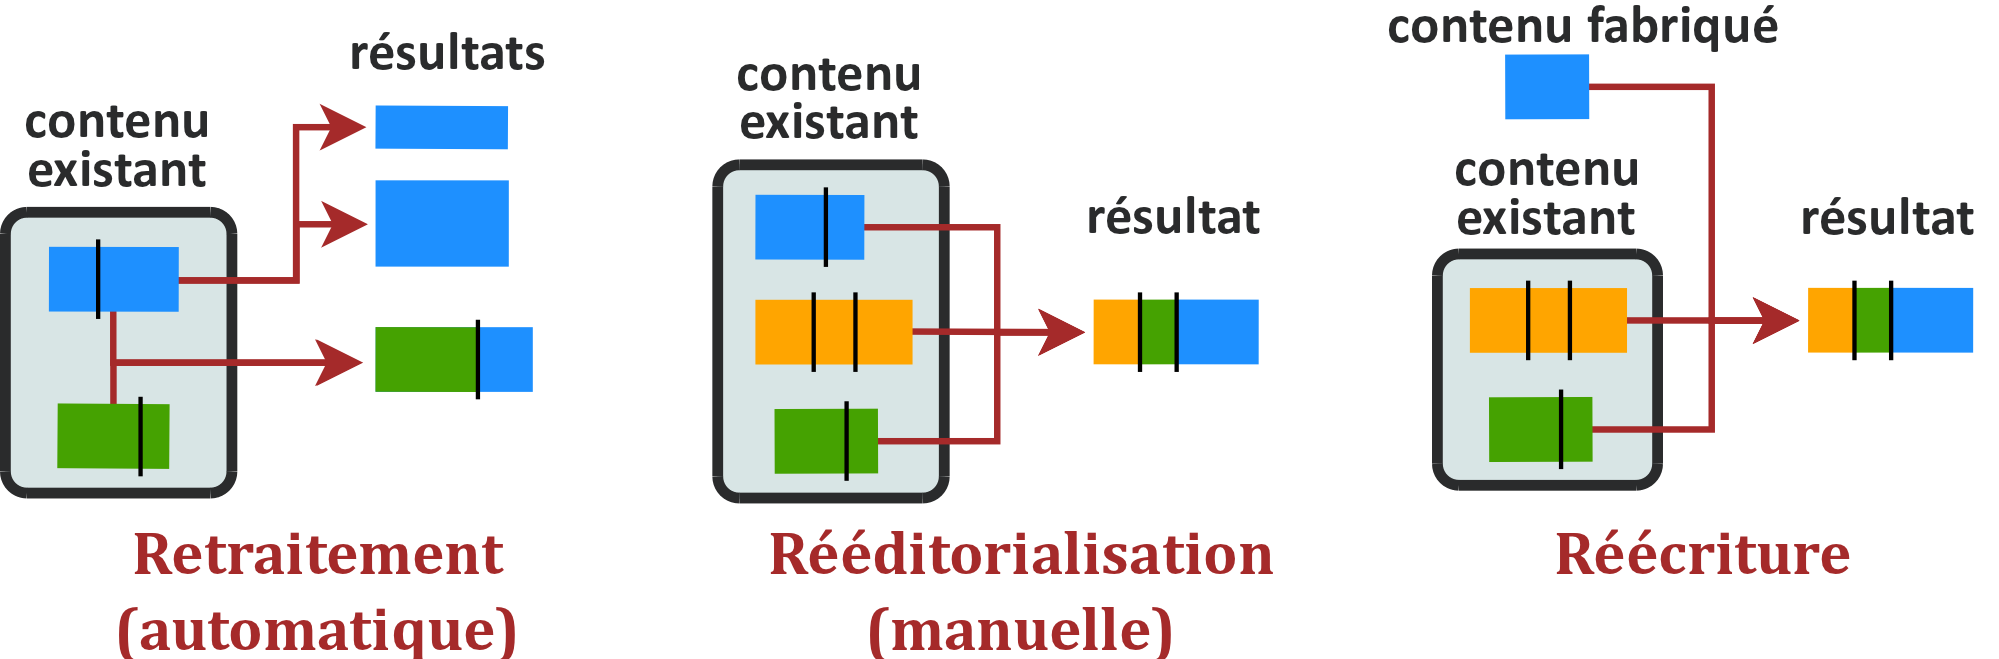
\includegraphics[width=0.75\textwidth]{images/Reuse-v1.png}
\caption{Les différentes pratiques de réutilisations}
\label{img:intro:reuse}
\end{figure}

Nous proposons donc de définir la terminologie suivante pour distinguer entre trois niveaux successifs de réutilisation, chacun visant à créer un nouveau document mais suivant des opérations différentes (voir Figure \ref{img:intro:reuse}). 
La premier critère distinctif est l'automatisation de la transformation, le second critère repose sur la création originale de contenu plutôt que la réorganisation d'un existant : 
\begin{liste}
	\item le \eg{retraitement} (repurposing) qui se caractérise par une automatisation de la transformation opérée sur le contenu (quelque soit son type), c'est-à-dire que cette transformation est effectué par un logiciel lui-même paramétré par un humain. 
	Ces transformations visent à modifier la forme d'expression du document, extraire des fragments de contenu de différentes sources pour les aggréger dans un nouveau document, ou bien encore réorganiser automatiquement la structure du contenu. 
	Le retraitement dépasse le polymorphisme en ce sens où il est possible de gérer de multiple sources de contenus pour construire dynamiquement un nouveau document. 
	Dans le cas de l'audiovisuel, il s'agit des pratiques de réencodage, de changements de format d'encapsulation etc.
	Pour reprendre l'exemple précédent (\ref{sec:ex-reuse}) d'un contenu TV pour une diffusion Web, ou bien encore la création automatique de résumé de rencontres sportives etc. \\

	\item la \eg{rééditorialisation} (reediting) se caractérise par une transformation (manuelle et automatique) de contenus existants. 
	Le document doit s'adapter à un nouveau contexte de lecture (genre éditoriale, public, forme d'expression etc.).
	La transformation du contenu nécessite une compréhension du nouveau contexte de lecture et consiste en des opérations de réorganisation, de mise en relation avec d'autres contenus, de traduction etc. 
	Ces opérations ne se limitent pas à une transformation de la forme d'expression du document (retraitement) mais ne constituent pas une création originale de contenus (réécriture). 
	Simplement, on réutilise divers contenus existants pour créer un nouveau document.  
	La ré-éditorialisation repose donc sur le polymorphisme et la réutilisation au sens de \cite{Crozat2011}.
	Dans le cas de l'audiovisuel, il s'agit typiquement de pratiques de re-montage et de nouvelles sélections de contenu. 
	Pour reprendre l'exemple précédent, il s'agit de monter différemment une séquence initialement prévue pour un journal TV et qui doit s'insérer dans un DVD etc. \\

	 
	\item la \eg{réécriture} (reauthoring) se caractérise par une transformation de contenus existants accompagnée d'une création de contenu original. 
	L'ajout de contenu sert à satisfaire soit aux attentes spécifiques du nouveau public cible, aux contraintes d'un nouveau genre éditorial (commentaires, explications, exemples etc.) soit à la création d'une version augmentée d'un document existant (pas de changement de public cible, mais de nouvelles attentes).
	Dans le cas de l'audiovisuel, il s'agit par exemple de la construction d'un documentaire à partir de vidéo d'archives, la création originale étant le commentaire proposé.\\	 
\end{liste}

Les pratiques de réutilisations sont donc chevillées aux dimensions techniques, éditoriales et sémiotiques du contenu audiovisuel. 
Leur mise en place pose également des problèmes dans l'organisation de la chaîne de production audiovisuelle et son informatisation
% Il faut donc élargir le champ de la modélisation des contenus à une dimension sémiotique et éditoriale et faire le lien avec le déroulement de la production.








%%%%%%%%%%%%%%%%%%%%%%%%%%%%%%%%%%%%%%%%%%%%%%%
\subsection{Évolutions de la chaîne de production}\label{sec:rechaine}
\e{
Les changements introduits par la réutilisation dans la chaîne de production sont donc plus vastes qu'une simple adaptation technique à de nouveaux modes de distribution. %(canal de diffusion + terminal de lecture). 
Il s'agit également de prendre en compte l'audience visée pour affiner encore plus l'adaptation du contenu à ses futurs consomateurs/lecteurs.
L'objectif est de favoriser le développement de variantes d'un même programme soit par la restructuration du contenu (retraitement ou rééditorialisation) ou par l'ajout de contenus (réécriture). 
L'introduction d'acteurs tiers dans une chaîne de production pour fabriquer ou fournir du contenu ne peut se faire sans une plus grande maîtrise des contenus et une meilleure description de ces derniers dès la pré-production.
En effet, le client qui souhaite déléguer la fabrication de contenu à un fournisseur tiers doit d'abord définir ses attentes. 
À l'inverse, si le fournisseur connaît son contenu le client lui a besoin d'un descriptif pour sélectionner les fragments les plus pertinents.
Ainsi, les chaînes de production des clients et des fournisseurs doivent évoluer pour gérer (fournir/acquérir) non pas juste du contenu, mais des descriptions (adjointes ou pas à du contenu) facilitant le travail de leurs partenaires (fabrication ou réutilisation).
}
% Le producteur-diffuseur rentre alors dans une dynamique d'adaptation de ces contenus.

Comme nous l'avons constaté en \ref{sec:electro}, le développement de l'électronique offre de nouvelles opportunités de production mixte, soit avec des amateurs, soit avec d'autres professionnels. 
Cependant, une organisation souhaitant profiter de ces opportunités devra réussir d'abord à encadrer ses partenaires et clarifier avec eux les termes de leurs accords. 
Ce qui auparavant pouvait se résoudre \e{de visu} ou de manière informelle doit maintenant être explicité afin de clarifier la demande, c'est-à-dire le contenu souhaité. 
Qu'il s'agisse de passer commande, ou bien de rechercher dans des bases existantes, cette étape s'apparente à la définition du besoin, à l'écriture d'un cahier des charges, ou dans les termes propres à la production audiovisuelle, au \e{Scripting} défini en \ref{sec:preprod}. 
Maintenant que la fabrication du contenu est déléguée à des tiers, il reste cependant à récupérer le résultat et à vérifier qu'il satisfait à la demande initiale. 
Cette dernière étape nommée généralement \e{Acquisition} constitue un travail à part entière puisqu'il s'agit de \gui{faire rentrer} le contenu dans les \gui{cases} du système d'information et de gestion des contenus. 
En plus des questions de formats informatiques, s'ajoute souvent le problème de la description des contenus et de leur classification en vue de leur utilisation future.  
L'acquisition dépend grandement des conventions établies avec le fabricant/livreur de contenu et impacte directement sur le temps passé à faire le \e{derushing}. 

Côté client, on transforme d'abord la phase de scripting en l'expression d'une \pc{Commande} ou d'une \pc{Requête} ce qui permet de déléguer la fabrication des contenus à un tiers.
Ensuite, on vérifie par \pc{Acquisition} du contenu que le résultat correspond bien à la demande et on procède aux ajustements nécessaires (si besoin) pour satisfaire aux contraintes de notre système (voir Figure \ref{img:intro:evochain}). 

\begin{figure}[ht!]
\centering
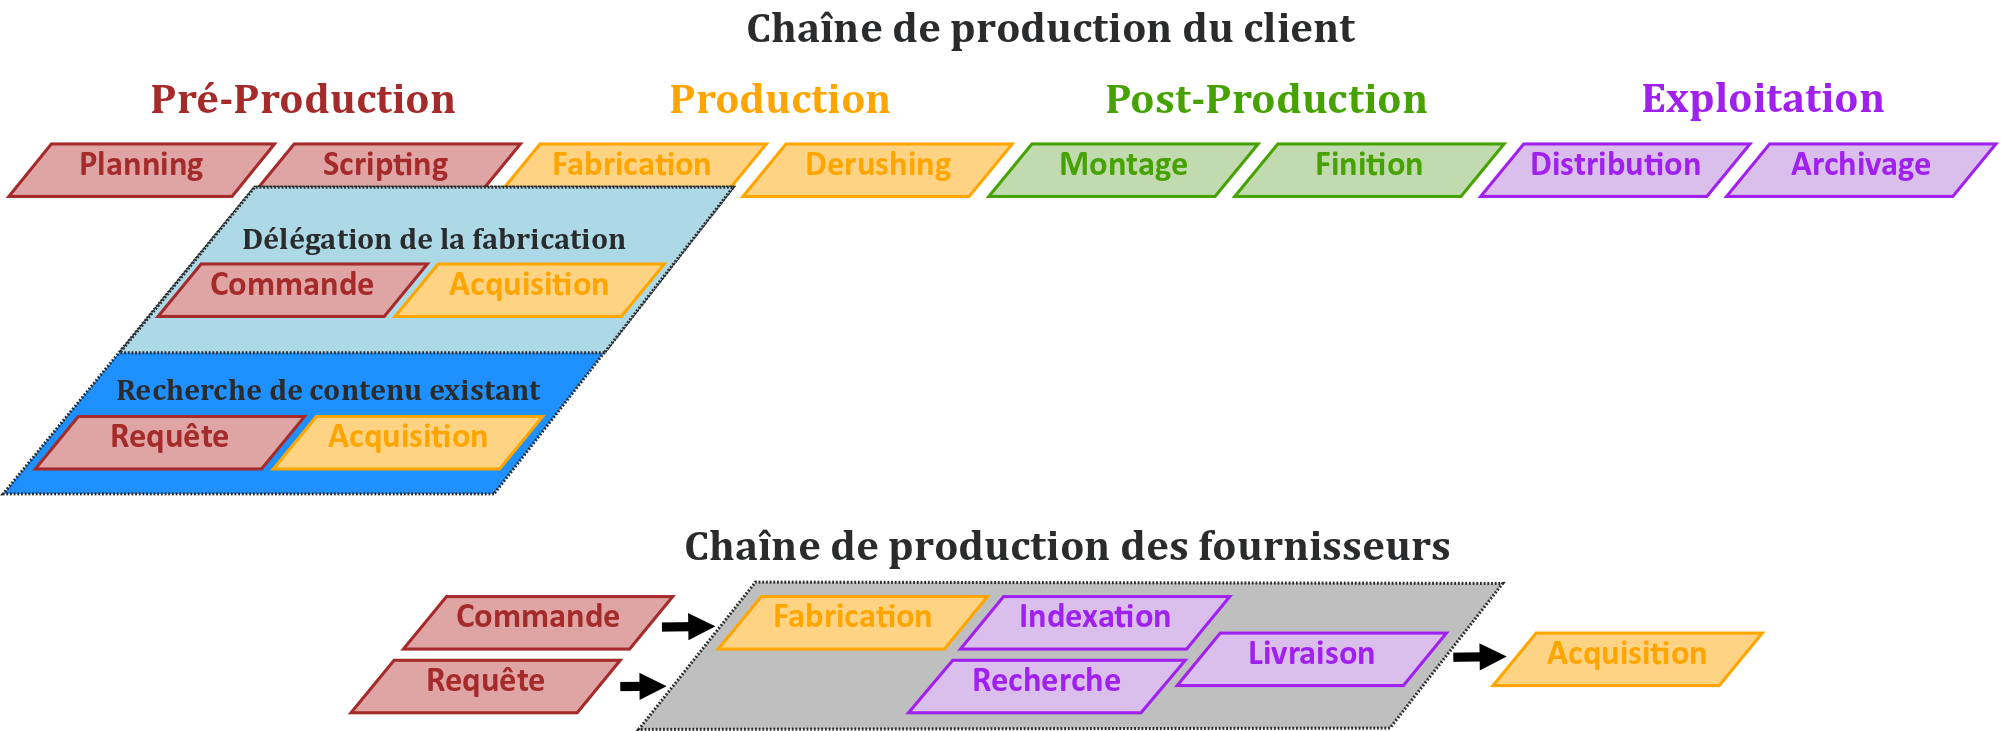
\includegraphics[width=\textwidth]{images/Workflow-Thesis-v6.png}
\caption{Ouverture des chaînes de production du client et du fournisseur}
\label{img:intro:evochain}
\end{figure}

Du côté des fournisseurs de contenu, il existe une distinction entre les chaînes du fabricant et du fournisseur du contenu :  

\begin{liste}
	\item \e{déléguer la fabrication à des contributeurs tiers} : l'utilisation du scripting pour définir la \pc{Commande} de contenu attendu semble une solution satisfaisante, à condition que le vocabulaire utilisé soit normé et rattaché à une conceptualisation de manière à éviter la confusion ou les différences d'interprétations. 
    Lorsqu'il s'agit d'amateurs, la situation se complique car on ne peut pas s'appuyer sur une conceptualisation commune de la production audiovisuelle pour clarifier la commande. 
    De plus, le manque d'expérience et l'ignorance des usages du métier impliquent non seulement de documenter les concepts par des mots et des définitions, mais aussi d'expliquer ce qu'il faut faire durant la phase de \pc{Fabrication}. 
    En d'autres termes, en travaillant avec des amateurs, les professionnels ne se retrouvent non pas à écarter la confusion entre des mots se reférant au même concept, mais à expliquer les opérations auxquelles ces concepts font référence. 
    De même pour l'acquisition, s'il s'agit surtout de se mettre d'accord entre professionnels, travailler avec des amateurs semble plus difficile de prime abord. 
    Les notions de formats d'encodage et d'encapsulation sont souvent confuses ou se mélangent, de même que la description des contenus peut s'avérer compliquée à réaliser sans expérience préalable. 
    Tout du moins, il faut remarquer que la description de la demande initiale sert de description a minima du contenu produit, même si les variations ou les écarts ne sont pas forcément indiqués.
    Le cas échéant, une phase d'\pc{Indexation} peut être nécessaire pour décrire le contenu suivant les exigences du client.\\

	\item \e{rechercher des contenus existants depuis les bases professionnelles} : l'utilisation du vocabulaire de l'écriture audiovisuelle pour définir une \pc{Requête} nécessite une indexation utilisant ce même vocabulaire, ou alors une manière de traduire la requête d'un langage à l'autre (par alignement des vocabulaires par exemple). 
	De même, il faut pouvoir s'accorder sur le niveau de fragmentation recherché (programme complet, séquences, scène, frame etc.), le format du contenu, les descriptions ou les métadonnées à fournir etc.
	Ainsi, la \pc{Livraison} de contenu ne consiste pas en un simple transfert de fichier, mais représente le moment où l'on teste l'interopérabilité entre les systèmes et les formats. 
	Cette étape est d'autant plus cruciale qu'elle se répercute directement sur la phase d'acquisition pour le client. 
	Tout ce qui n'a pas pu être résolu à la livraison (côté fournisseur) devra l'être au moment de l'acquisition dans le système (côté client).\\
	% un vocabulaire de requêtes, s'accorder sur les niveaux de fragmentation, le format de livraison, le contenu de la livraison
\end{liste}



Finalement, il nous faut encore éclairer à quels moments dans la chaîne de production les différentes pratiques de réutilisation sont réalisées (voir définition en \ref{sec:reuse}).
De manière générale, on considère que la réutilisation commence à la phase de pré-production, au moment du \pc{Planning} et du \pc{Scripting} où l'on spécifie les nouvelles formes et formats d'exploitation (voir Figure \ref{img:intro:reutilisation}). 
Mais chaque pratique opére à différents étapes de la chaîne :
\begin{liste}
	\item pour le \e{retraitement}, les variations sur la forme d'expression du document se réalisent en phase de \pc{Finition}. 
	C'est à ce moment que l'original et les variantes sont encodés et encapsulés dans les formats correspondants à leur mode de distribution. 
	Lorsqu'il y a manipulation de la structure des contenus, ces opérations (automatisées) se réalisent à la phase de \pc{Montage}.

	\item pour la \e{rééditorialisation}, le travail commence en phase de \pc{Derushing}, par la sélection des séquences de contenu à ajouter ou à retirer du contenu original. 
	La grande différence avec le retraitement, c'est que cette sélection s'effectue manuellement sur les contenus à disposition. 
	Ensuite, on opére un nouveau \pc{Montage} qui peut également impliquer une \pc{Finition} différente.

	\item pour la \e{réécriture}, la grande différence avec les autres pratiques est que l'on ajoute une nouvelle phase de \pc{Fabrication}. 
	Qu'il s'agisse de création originale ou de récupération de contenu chez un fournisseur tiers, la réécriture consiste à utiliser de nouveaux contenus. 
	Ensuite, on sélectionne en \pc{Derushing} les séquences qui permettront de réaliser un nouveau \pc{Montage}. 
	Finalement, plusieurs \pc{Finition} sont à envisager suivant les cas d'exploitation.
\end{liste}
% conséquences de la réutilisation dans la chaîne : à quel étape ça se joue

\begin{figure}[ht!]
\centering
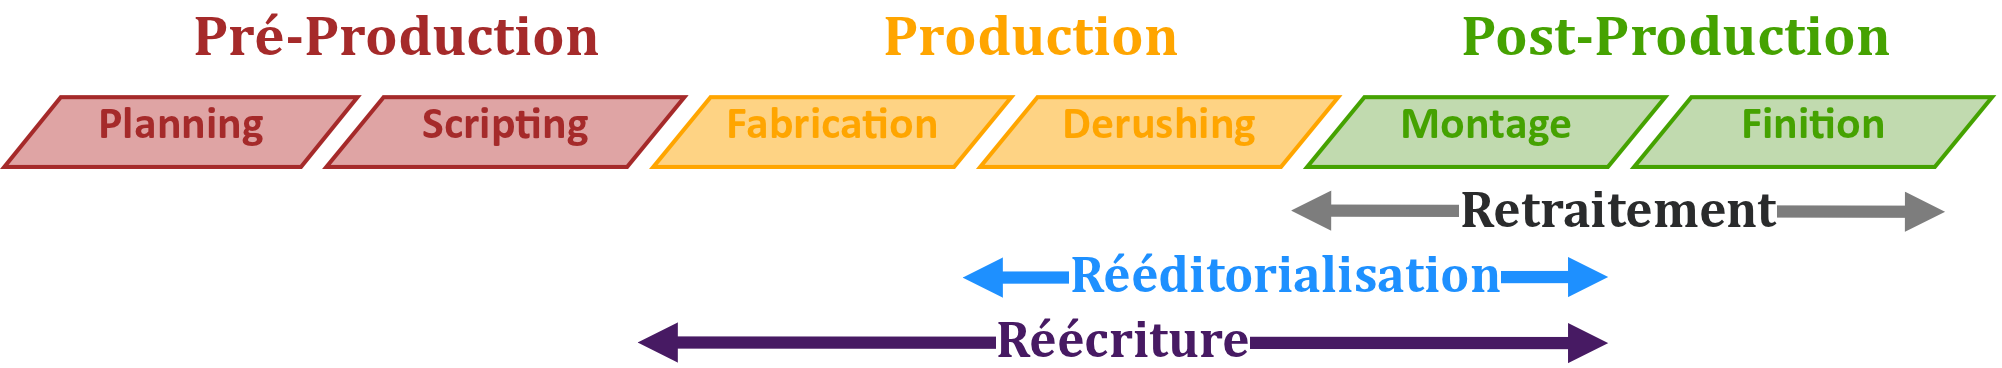
\includegraphics[width=0.8\textwidth]{images/Workflow-Reuse-v1.png}
\caption{Les différentes formes de réutilisation et leur mise en oeuvre dans la chaîne de production audiovisuelle.}
\label{img:intro:reutilisation}
\end{figure}








\subsection{Formats conteneurs pour l'audiovisuel} \label{sec:wrapper}
% intro
Les formats conteneurs sont des formats de fichiers qui encapsulent des contenus de toutes sortes (audio, vidéo, texte, image etc.). 
Un des exemples le plus connu pour la vidéo est le format AVI de Microsoft, souvent confondu avec un format de compression. 
Ces formats ont la particularité d'associer aux contenus audio-visuels des informations annexes, le plus souvent sous la forme de métadonnées.
L'intérêt de ces formats est de constituer un objet numérique qui structure l'enregistrement du contenu et de ses informations annexes et fournit ainsi une manière unique d'y accéder (\cite{Ferreira2010}).
Sans cela, les informations seraient dispersées et le lien avec le contenu devrait se faire via des références. 
Cette force constitue également un inconvénient lorsqu'il n'est pas possible de faire évoluer le modèle d'information ou bien d'en changer en fonction du type de production ou d'exploitation envisagé.

Dans le cas de la production télévisuelle, deux formats liés et complémentaires ont été progressivement adoptés par l'industrie.  
Il s'agit du \pc{Material eXchange Format} (MXF) et de l'\pc{Advanced Authoring Format} (AAF) que nous présentons par la suite. 
Leur particularité est de pouvoir intégrer des schémas de métadonnées propres aux besoins de l'industrie, mais aussi de pouvoir en utiliser d'autres. 
Comme ces formats servent de référence à l'industrie, il est particulièrement intéressant pour nous de comprendre leur modélisation de l'objet audiovisuel, de voir comment ils gèrent les résultats intermédiaires de la chaîne de production ou quels genres d'informations ils embarquent avec le contenu.


\subsubsection{Material eXchange Format}\label{sec:mxf}
% qui / quand
MXF est un format conteneur ouvert développé depuis le milieu des années 90 par des membres de l'industrie et standardisé en 2004 par la \pc{Society of Motion Picture and Television Engineers} (SMPTE).
% objectif
Son objectif est de favoriser les échanges de contenus audio-visuels finis en les associant à d'autres données ou métadonnées (\cite{Devlin2002}).
Ces métadonnées sont structurés par le schéma \pc{Descriptive Metadata Scheme-1} (DMS-1, ) que nous présenterons en détails dans la suite de la section. 

% description
Voici d'abord les principales caractéristiques de MXF en tant que format (\cite{Ferreira2010a}) : 
\begin{liste} 
	\item \e{indépendant d'un système propriétaire}. 
	Le standard se veut avant tout un format qui fonctionne sur tout systèmes. 
	Ainsi, il définit une organisation des données bit par bit qui repose notamment sur le système de \pc{Key-Length-Value} (KLV, clé-longueur-valeur). 
	La clé donne un identificateur de l'élément à suivre, la longueur précise la taille de la valeur à suivre et la valeur contient les données de l'élément.
	Comme dans tout format de fichier, on retrouve la définition d'en-tête et de fin de fichier. 
	L'en-tête contient des métadonnées de description du contenu (\pc{Header Metadata}), de sa structuration (\pc{Partition Metadata}) et une table d'association entre un timecode et une position dans le flux binaire du fichier (\pc{Index Table}).

	\item \e{indépendant des méthodes de compression du contenu utilisées}.
	MXF définit une structure d'encapsulation et d'accès au contenu nommé \pc{Essence Container} (EC) qui permet de transporter du contenu sans le transformer ou bien de faire référence à des fichiers externes.  
	MXF possède des transpositions permettant de synchroniser différents flux de contenus, quelque soit leur encodage. 
	Chaque type de contenu est traité à part, ainsi les EC sont composés de \pc{Content Package}, eux-mêmes décomposé en \pc{Picture Item} (piste vidéo), \pc{SoundItem} (piste audio), \pc{Data Item} (télétexte, sous-titre etc.), \pc{Compound Item} (contenu audiovisuel encodé comme un seul contenu) et \pc{System Item} (autres données comme les timecode etc.).
	La Figure \ref{img:mxf-content} montre deux méthodes d'encapsulation de ces essences.


	\item \e{diffusable en flux continu ou bien par fichier}. 
	Suivant la méthode d'organisation de l'EC décrit ci-dessus, le contenu d'un fichier MXF peut être visionné au cours de son transfert (streaming). 
	Cette caractéristique est particulièrement importante dans le cadre de la diffusion télévisuelle et s'applique à tout les types de contenu d'un MXF (audio-visuel, mais aussi sous-titre ou métadonnées etc.). 
	Naturellement, le fichier MXF peut également être transféré en FTP.

	\item \e{une organisation des contenus indépendante de leur visionnage}. 
	En effet, MXF définit à part l'organisation des contenus encapsulés et la manière de les visionner.
	Le \pc{Header Metadata}	d'un fichier MXF contient une partie \pc{File Pacakage} (FP) qui décrit la manière dont les fichiers de contenus sont encapsulés dans le MXF. 
	Cette description détaille les méthodes d'encodage pour toutes les pistes de contenus (Track) du fichier, de même que les timecode originaux.
	Cependant, si le FP décrit les sources d'un fichier MXF, il existe également un \pc{Material Package} (MP) décrivant la manière dont celles-ci doivent être visionnées.
	Il s'agit là de définir un montage simplifié qui explicite quelle partie et dans quel ordre jouer les contenus sources, à la manière d'une \ciel{Edit Decision List}. 

	\item \e{encapsulation conjointe des contenus et des métadonnées}. 
	Comme nous l'avons vu, un fichier MXF contient un \pc{Header Metadata} transportant des métadonnées propres à l'ensemble du fichier ainsi que des métadonnées propres à chaque paquet de données (Package). 
	Ces éléments sont donc intégrés dans la structure du fichier, au même titre que le contenu.
\end{liste}


\begin{figure}[ht!]
\centering
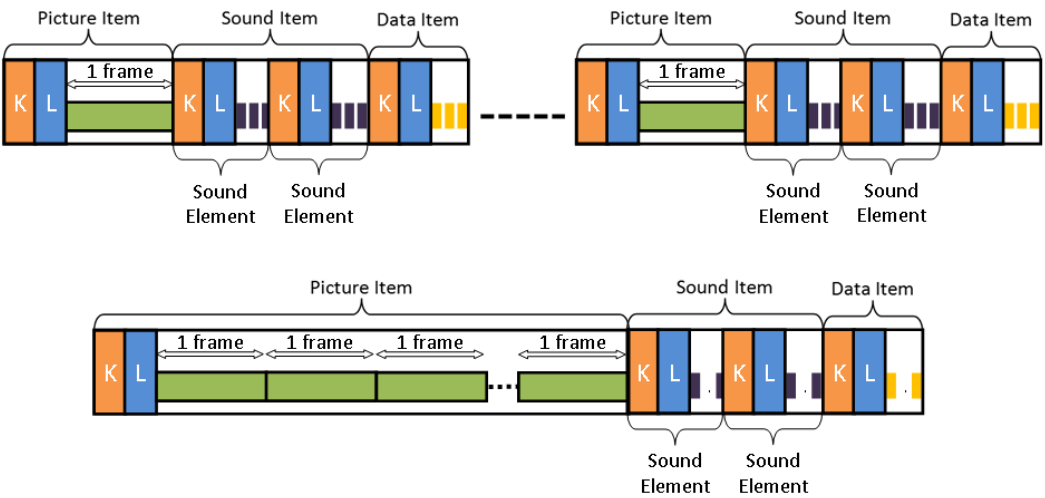
\includegraphics[width=0.9\textwidth]{images/MXF-ContentPackage.png}
\caption{Deux méthodes d'encapsulation des essences en MXF : image par image (haut, pour le streaming), par séquence vidéo (bas).}
\label{img:mxf-content}
\end{figure}

\paragraph{Adoption et usage}
Du fait de sa large adoption par l'industrie de la télévision, il favorise l'interopérabilité entre les systèmes, souvent propriétaires, des producteurs, diffuseurs, chaînes de télévision etc. (\cite{Ferreira2010}, \cite{Devlin2002}). 
Cependant, MXF n'est pas fait pour gérer les résultats intermédiaires de la chaîne de production. 
Il a été spécifiquement conçu pour favoriser la circulation des programmes finis, indépendamment de la manière dont les contenus sont matériellement enregistrés et structurés.
De ce fait, MXF se positionne comme un format utilisé en fin de chaîne de production, à la diffusion des programmes ou bien dans le cas d'échanges entre professionnels.

\subsubsection{Description Metadata Scheme-1}\label{sec:dms-1}
Le schéma DMS-1 a été standardisé par le SMPTE en 2004 (\cite{Smpte2004}).
Il propose trois schémas de description (\pc{Framework}), chacun proposant une perspective de description particulière : 
\begin{liste}
	\item le \pc{Production Framework} propose une description du fichier MXF en tant que résultat d'une production. 
	Les informations qu'il regroupe s'appliquent donc au fichier en entier (identification, propriété intellectuelle, droits et contrats, projet, format de publication, format d'image, récompense) mais aussi au contenu de l'objet audiovisuel (évènements relatés, période historique, annotation).

	\item le \pc{Clip Framework} aborde la description du point de vue de la création du matériel audio-visuel, c'est-à-dire des séquences de contenu encapsulées dans le MXF. 
	On retrouve des informations liées à la production (projet, droits et contrat) mais surtout des éléments pour décrire les essences (format de l'image, sous-titre, script utilisé, matériel utilisé et paramètrage, opérations de transformation des essences) et une description par plan.

	\item le \pc{Scene Framework} propose une vision éditoriale du contenu en le découpant en scène et plan. 
	Ces éléments sont ensuite décrits en terme d'évènements, en précisant les participants et les lieux où ils se déroulent etc.
\end{liste}

\paragraph{Framework et ensemble de métadonnées}
Ces \pc{Framework} sont composés de petits ensembles de métadonnées, parfois partagés,  que l'on attachent au \pc{Header Metadata} d'un fichier MXF. 
Par exemple, l'ensemble \pc{Titles} est commun au trois \pc{Framework} et se compose des métadonnées suivantes ; \e{Extended Text Language Code} ; \e{Main Title} ; \e{Secondary Title} ; \e{Working Title} ; \e{Original Title} ; \e{Version Title}. 
De nombreux autres ensembles sont partagés, comme les annotations, la description des lieux, des participants, des organisations etc. 
Ces ensembles prennent alors un sens différent en fonction du \pc{Framework} auquel ils sont associés. 
Par exemple, on distingue les participants à la production, à la création d'une séquence, en tant que présentateur ou acteur (respectivement pour le \pc{Production}, \pc{Clip} et \pc{Scene Framework}). 
De même, pour les lieux il peut s'agir d'un lieu où se trouve l'organisme producteur, du lieu de tournage, du lieu où se déroule l'action qui est différent du lieu de tournage dans le cas d'une fiction (respectivement pour le \pc{Production}, \pc{Clip} et \pc{Scene Framework}). 
Ainsi, la distinction entre éléments réels (issu du \pc{Clip Framework}) ou fictifs (issu du \pc{Scene Framework}) n'est pas clairement spécifié. 
De manière générale, il semble regrettable que les mêmes ensembles de métadonnées soient utilisés pour décrire des objets différents.
Cela propage ainsi une certaine confusion sur le plan sémantique. 

\paragraph{Framework et Package MXF}
Comme pour les ensembles, les \pc{Framework} peuvent s'attacher à un ou plusieurs des \pc{Package} de MXF (\pc{File Package}, \pc{Material Package} etc.). 
Par exemple, le \pc{Clip Framework} appliqué au \pc{Material Package} décrit ce qui est nécessaire au visionnage du contenu (format d'image prévu).
S'il s'appliquait au \pc{File Package}, les informations correspondrait aux informations de création (format d'image original).
Là encore, l'objet de la description change légèrement et si les mêmes éléments de description peuvent être utilisé, il semblerait plus clair de préciser la nature de ces informations. 

Nous remarquerons que DMS-1 utilise la notion de plan de deux manière différentes qui peuvent sembler ambigüe. 
Ainsi, le plan est utilisé à la fois dans le \pc{Clip Framework} et le \pc{Scene Framework}. 
D'après les auteurs, cela correspond à la nature duale des plans, à la fois élément factuel et éditorial. 
Ce choix implique alors que chaque plan peut être décrit à deux endroits à la fois, selon deux perspectives différentes (descriptive de ce qui est perçu, ou bien pour nommer le plan par rapport au script par exemple).

\paragraph{Multilingue et thésaurus}
Concernant la gestion des vocabulaires et des langues, DMS-1 prévoit que certains ensembles de métadonnées soient décrites par un code de langue et puissent faire référence à un élément d'un thésaurus.
Cette perspective est particulièrement intéressante vis-à-vis des besoins que nous avons exprimés dans le chapitre précédent (\ref{sec:bm}).
Cependant, le lien avec un thésaurus externe est limité car il ne s'applique qu'aux ensembles et non à chaque métadonnée de l'ensemble.

\paragraph{Travaux liés}
\cite{Marcos2009} ont construit une ontologie basée sur le schéma DMS-1, MPEG-7 et une ontologie de domaine pour construire un système de Media Asset Management. 
Ce système, développé dans le cadre du projet européen RUSHES, a pour objectif d'aggréger des informations récoltées pendant la production par différentes sources, puis de les associer aux objets audiovisuels et proposer des services de recherche d'information et d'accès au contenu (\cite{Gorka2008}). 
Les objets audiovisuels considérés sont les prises de vue brutes, nommées \ciel{rush} dans le milieu audiovisuel.

L'approche consiste à transformer ou relier des informations de bas-niveau en une indexation sémantique à l'aide des ontologies développées.
Les services sémantiques proposés par le système sont les suivants : 
\begin{liste}
	\item \e{transformation de formats des données échangées pendant la production}. 
	Les annotations recueillies à partir des équipements de tournage et après analyse automatique du contenu sont transformés du format DMS-1 en un autre format utilisé par le système d'indexation.
	\item \e{sémantisation de l'analyse automatique du contenu}. 
	Les auteurs prennent l'exemple d'une reconnaissance des visages qui permet d'identifier le nombre de personnes présents dans une séquence.
	Ces personnes peuvent alors être intégrées à une base de connaissances.
	De même, l'analyse permet de détecter les changements de plans.
	\item \e{recherche, découverte, annotation de séquences}. 
	La recherche peut se faire soit à l'aide de mots-clés, soit à l'aide des concepts de l'ontologie, qui permettent alors d'enrichir les requêtes, de proposer des recommandations etc. 
	De plus, l'ontologie peut être également utilisé pour relier les annotations manuelles avec des concepts ou des éléments de la base de connaissances.
\end{liste}

Ces travaux poussent ainsi l'utilisation de DMS-1 en tant que schéma de description des prises de vue, juste après leur production, et non pas seulement des programmes finis, en fin de chaîne. 
Ce changement de granularité montre l'importance du \pc{Clip Framework} et du \pc{Scene Framework} qui permettent d'attacher la description à ces objets intermédiaires de la production.
Ceci est d'autant plus pertinent que DMS-1 prévoit déjà de décrire, en partie, les participants de la chaîne et leurs contributions.

L'originalité de l'approche se situe également dans la transformation des résultats d'une analyse automatique en objet sémantique. 
Les exemples de l'analyse des visages et de la détection de plan sont éclairants mais les auteurs ne fournissent pas d'indication pour généraliser le procédé à d'autres types d'information.



\subsubsection{Advanced Authoring Format}
% \cite{Gilmer2002} 
% \cite{Austerberry2004}
% qui 
AAF est un format conteneur développé principalement par l'\ciel{Advanced Media Workflow Association} (AMWA) en collaboration avec d'autres organismes tels que le SMPTE et l'EBU.
% objectif, portée et usage 
Ses objectifs sont similaires à celui de MXF, à la différence qu'AAF vise à favoriser les échanges de contenus à l'intérieur de la chaîne de production (\cite{Austerberry2004}).
AAF s'occupe plus particulièrement des informations utilisées au moment de la post-production par les applications de montage : 

\ciel{The traditional workflow – based around tape interchange, isolated non-linear editing and authoring tools, and ad-hoc metadata systems – is being recast as a more integrated networked system with a consistent approach to the format and interchange of essence and metadata.} (\cite{Gilmer2002})

% description
Le modèle de MXF présenté précédemment est en réalité une sous-partie de celui d'AAF. 
On retrouve donc les mêmes principes et fonctions, dont les \pc{Packages} qui portent les descriptions et les \pc{Items} qui encapsulent les contenus. 
Parmi les éléments supplémentaires dans AAF qui le destine particulièrement à une utilisation dans la chaîne de production., nous trouvons :
\begin{liste}
	\item le \pc{Physical Source Package} permet de référencer des contenus enregistré sur d'autres mediums que les disques durs (cassette vidéo, bande 35mm etc.).

	\item le \pc{Composition Package} permet de définir la manière dont le contenu doit être visionné en termes d'ordre (comme MXF) mais aussi en terme d'effets, de transition ou de composition des flux de contenu (ce que l'on appelle des EDL complexes).
	
	\item le \pc{Dictionary} qui permet d'intégrer des définitions des métadonnées autres que celles du dictionnaire du SMPTE dans le AAF.
\end{liste}

De plus, AAF se différencie par l'utilisation de la technologie \e{Structured Storage} de Microsoft pour gérer l'organisation des données (plutôt que la méthode du KLV).
De ce fait, AAF ne permet pas la diffusion en continu (streaming) de ses contenus.
Cependant, les deux formats utilisent le même modèle de structuration, ce qui permet aux applications d'effectuer des transformations de l'un à l'autre aisément, et particulièrement du AAF vers le MXF en suivant le déroulement de la chaîne.
Leurs différences les prédisposent néanmoins à des usages complémentaires. 
AAF se positionne comme un format pour la post-production qui conserve toutes les sources et le master alors que MXF, avec son modèle simplifié et ses capacités de diffusion en continu, est particulièrement intéressant pour les échanges de programmes finis.


\paragraph{SMPTE Metadata Dictionary}
Ce dictionnaire est un gigantesque registre de toutes les métadonnées utilisées par l'industrie télévisuelle. 
Régulièrement mis à jour, la dernière version disponible (\cite{SMPTE2010}) comporte 1476 métadonnées distribuées dans 499 catégories et sous-catégories.
La nature des métadonnées est très diverse, puisqu'on trouve des identificateurs, des informations administratives, interprétative, paramétriques, liées au processus etc.
Le dictionnaire donne une identification unique à chaque métadonnée et donne une définition ainsi que le codage utilisé pour la valeur. 
Malgré sa taille imposante, il est utilisé par les membres de l'industrie et notamment dans DMS-1.



\subsection*{Discussion}
\addcontentsline{toc}{subsection}{Discussion}
Les formats conteneurs MXF et AAF reposent sur le schéma de description DMS-1 ainsi que des dictionnaires de métadonnées développés par l'industrie.
L'originalité de ces formats est d'associer directement au matériel audiovisuel plusieurs perspectives de modélisation (\pc{Framework}) [\g{$\chi_1$ : autonomie}].
L'objet audiovisuel est ainsi modélisé en tant que résultat d'une production qu'il faut valoriser commercialement (\pc{Production}) ; 
décomposé en éléments narratif (plan, scène) faisant partie d'un ensemble documentaire (\pc{Scene}) et dont on décrit le contexte historique (\pc{Production}) et les évènements réels (\pc{Clip}) ou fictifs (\pc{Scene}) qui s'y déroulent ; matériel audiovisuel construit pendant la production dont on décrit les caractéristiques techniques (\pc{Clip}).
Cette pluralité des points de vue pourrait permettre de modéliser les produits intermédiaires de la chaîne tout en leur associant des métadonnées. 
Ce remplissage progressif ne peut intervenir qu'après la production du matériel, et encapsulé dans le format AAF. 
C'est donc les informations de la post-production qui y sont capturées, puis transmises sous une forme simplifiée à un MXF qui symbolise le produit final de la chaîne.
Les produits intermédiaires ne sont donc pas représentés pour eux-mêmes, mais en tant que partie du produit final.
L'approche de modélisation est donc intéressante, mais le couplage matériel et métadonnées empêche de fragmenter la modélisation et de la commencer dès le début de la production.

Parmi les descriptions associées au matériel audiovisuel [\g{$\chi_2$ : réutilisabilité}], on note un certaine confusion sur le plan sémantique. 
Ainsi, des mêmes ensembles de métadonnées sont utilisées pour représenter des éléments fictifs ou rééls, tandis que d'autres peuvent prendre un sens différents suivant le \pc{Package} ou le \pc{Framework} auxquels ils sont associés.
Ainsi, il ne s'agit pas de critiquer la modélisation qui distingue élément réél et fictif, ou bien encore le plan prévu dans le script et le plan tourné, mais bien la représentation confuse qui en est faite dans DMS-1.

Nous en concluons que les formats conteneurs sont adaptés à la circulation de documents audiovisuels finis mais dont la représentation d'une seule pièce et parfois confuse ne couvre pas nos besoins pour la réutilisation de fragments documentaires.

%====================================================
%====================================================
%====================================================
\newpage
\section{Déscription des objets audiovisuels}\label{sec:desc}
\e{
Avant de commencer notre état de l'art sur les modélisations des objets audiovisuels, nous souhaitons préciser la nature des descriptions et les approches de fabrication de ces descriptions (\ref{sec:fab}).}
% Nous verrons quelles types de description chacune de ces approches construit sur les contenus, et comment ces descriptions sont exploitées, pour quel type d'usage, à l'intention de systèmes informatiques ou d'être humains.

\subsection{Fabriquer des descriptions}\label{sec:fab}
% \subsection{Quelles descriptions ?}

\subsubsection{Nature des descriptions}
\paragraph{L'intérêt des descriptions textuelles}
Tout d'abord, nous souhaitons argumenter sur les avantages d'une description textuelle de contenus audio-visuels. 
En effet, pourquoi ne pas se contenter de ce que les images ont à nous offrir pour construire des index et rechercher ces images ? 
La question est d'autant plus pertinente que depuis presque une vingtaine d'années se développent des techniques évaluant la similarité entre images, ce qui permet d'utiliser une image (\gui{Query by Example}, initié par \cite{Flickner1995}, \cite{Pentland1996}) ou bien une représentation graphique (\gui{Query by Canvas}, initié par \cite{Flickner1995}, \cite{Bach1996}) comme élément de base pour une requête.
Ces approches sont donc tout à fait pertinentes dans le cadre de la recherche d'images extraites d'objets audiovisuels. 
Cependant, ces techniques reposent sur une caractérisation visuelle de l'image qui ne suffit pas à rendre compte de la richesse d'information que l'on voudrait associer aux objets audiovisuels.
En effet, de lui-même le contenu audiovisuel ne se laisse pas saisir dans son entièreté, ni ne se laisse manipuler aussi aisément que nous arrivons à le faire avec du texte. 
L'objet audiovisuel est avant tout temporel, il se déploie progressivement au fur et à mesure de sa lecture. 
On ne peut donc l'appréhender qu'en prenant le temps de le voir, instant après instant. 
À l'inverse, le texte est déployé dans l'espace ce qui lui permet d'être observé d'un point de vue synoptique. 
Ensuite, l'informatique manipule  bien plus aisément le texte que les contenus audiovisuels, surtout du point de vue de l'indexation. 
L'indexation textuelle utilise des mots-clés extraits directement du texte, mots-clés que l'on a appris à utiliser également pour effectuer une recherche d'information. 
De plus, les mots peuvent servir à décrire de multiple aspects de l'objet audiovisuel, qu'il s'agisse de nommer des éléments de l'image, de décrire sa composition, le contexte de sa production, son statut légal etc.
La limite d'une telle approche ne semble ainsi pas provenir du langage utilisé pour exprimer ces mots, mais plutôt de la manière de produire ces libellés. 
Nous écartons donc de notre état de l'art les recherches par images pour nous concentrer sur l'étude des modèles de description permettant de prendre en compte plusieurs aspects de l'objet audiovisuel. 


\paragraph{La diversité des descriptions}
La description d'un objet dépend fortement du point de vue de la personne qui la produit. 
En particulier, chaque corps de métier de la chaîne de production peut avoir une perspective particulière sur l'objet audiovisuel, même s'ils partagent des éléments communs pour discuter de sa production. 
Comme ces informations peuvent servir à de nombreux usages, il est intéressant de proposer des catégories permettant de les distinguer. 
Ainsi, \cite[\S 2:Types of Metadata]{Austerberry2004} distingue en particulier trois types d'informations : 
\begin{liste}
	\item \ciel{descriptive information} (informations descriptives) : qui sont relatives à la description du contenu, comme le sujet ou le genre de l'objet audiovisuel. 
	Par exemple, on peut associer des noms propres, des lieux, des évènements etc. à l'objet en fonction de ce dont traitera le contenu audiovisuel. 
	Un vocabulaire contrôlé peut servir à indiquer le "genre" de l'objet, c'est-à-dire les règles de genre qu'il suit au niveau de la structure, du ton etc.
	De même, des résumés textuels peuvent être inclus, à la manière de ceux prévus pour les guides TV. 

	\item \ciel{administrative information} (informations administratives) : qui relèvent de l'aspect métier et légal de la production de l'objet audiovisuel. 
	On cherchera à lister les contributeurs à la production de l'objet ainsi que les détenteurs de droits d'utilisation sur l'oeuvre. 
	Ces informations peuvent servir à retrouver des objets audiovisuels, notamment dans le cas de professionnels.
	Il peut également s'agir d'informations confidentielles comme les contrats de la distribution indiquant les droits d'utilisation de l'oeuvre, ou bien les contrats liées à la production. 
	Ces informations ne décrivent donc pas le contenu des objets audiovisuels, mais servent à faciliter leur gestion et leur exploitation future.

	\item \ciel{preservation information} (informations de conservation) : qui visent à faciliter la conservation et la réutilisation des objets et des fragments audiovisuels. 
	Il s'agit de pouvoir conserver des informations afin de faciliter la réutilisation de prises de vue dans de nouveaux contextes, de nouveaux montages ou bien de versions spéciales suite à un changement de support de distribution. 
	De plus, cela peut aussi concerner le suivi des conditions de stockage des objets audiovisuels (lieux, support, état etc.) ou bien la réalisation d'opération de restauration. 
	Il s'agit donc d'informations qui permettent d'identifier et de pister non seulement les objets audiovisuels finis, mais également tous les fragments qui ont été crées à l'occasion et toutes les versions qui ont été construites par la suite.
\end{liste}


Nous pouvons ajouter à ces catégories, d'autres types d'informations proposées par \cite{Rayers2002} : 
\begin{liste} 
	\item \ciel{compositional information} (informations de composition) : qui identifient la liste des fragments composant un objet audiovisuel et la manière dont ils doivent être montés pour reconstruire l'objet. 
	Dans le milieu de l'audiovisuel, ces informations sont représentées sous la forme de ce qu'on appelle une \ciel{Edit Decision List} (EDL).
	Cette liste peut être produite soit sous forme papier, soit par un logiciel de montage en utilisant une des dizaines de formats existants, formats souvent propriétaires et liés au logiciel de montage. 
	Ces informations servent à décrire la structure des objets audiovisuels et peuvent servir à leur gestion.
	Elles sont à rapprocher des \ciel{preservation information} dans le sens où elles permettent de garder une trace du montage. 


	\item \ciel{technical or essential information} (informations techniques) : qui correspondent à une description technique des caractéristiques du signal audio-visuel. 
	Ces informations sont généralement présentes dans les formats d'encapsulation de contenu numérique afin de permettre son décodage.
	Ces informations peuvent également servir à différencier plusieurs versions d'un objet audiovisuel qui ne varieraient que par leur encodage. 
	Il s'agirait alors de rapprocher ces versions avec leur utilisation futures (utilisation comme proxy, version destinée à un support particulier, à un canal de distribution etc.).
\end{liste}


Notons enfin, qu'il existe également toutes sortes de descriptions produites par des intervenants extérieurs à la chaîne de production (les spectateurs, les critiques, les sémiologues etc.), qui sont autant d'analyse pouvant se représenter sous la forme d'une structuration documentaire (voir \ref{sec:uc-sd}).
% pertinent pour notre problème.



\subsubsection{Fabriquer les descriptions, \e{endogènes} ou \e{exogènes} ?}\label{sec:codesc}
Nous distinguons deux méthodes de fabrication des descriptions suivant le moment où l'information est construite.
Les méthodes \e{exogènes} interviennent en fin de chaîne, lorsque l'objet audiovisuel est constitué et que l'on souhaite appliquer une méthode d'analyse. 
À l'inverse, les méthodes \e{endogènes} correspondent à la collecte d'information pendant la production. 
Ces méthodes s'arrêtent généralement au moment de la fabrication du matériel et se concentrent sur les informations contenues dans le script. 
Pour cela nous les nommons \e{a priori} (avant la fabrication), et nous les opposons à une méthode \e{dynamique} que nous souhaitons développer, et qui poursuit la collecte tout au long de la production.


% \subsubsection{La collecte durant la production}
\paragraph{Fabrication \e{endogène}, la collecte durant la production}
Dans la chaîne de production audiovisuelle, chaque communauté de contributeurs a un intérêt particulier et souvent différent sur les informations à partager sur l'objet. 
Les informations que l'un jugera critique (le numéro de la cassette qui contient la prise de vue n°354) peuvent être jugées insignifiantes pour d'autres (un journaliste se contentera de savoir que la prise de vue existe alors que cette information est capitale pour la régie). 
Il existe donc autant de descriptions possibles d'un objet, que de points de vue sur cet objet. 
De plus, une description n'est jamais utile qu'en fonction d'un usage. 
Savoir où se trouve la prise de vue n'a d'intérêt que pour la personne qui devra en réaliser le montage, ou bien s'assurer de la préservation de la cassette une fois utilisée. 
Les professionnels de la production sont donc confrontés à de multiples informations, pas forcément pertinentes par rapport à la tâche qu'ils doivent réaliser mais qui peuvent s'avérer utiles plus loin dans la chaîne.  

\citeauthor{Rayers2002}, comme \citeauthor{Austerberry2004} présentent en détails la manière dont les informations sont produites dans les processus de production télévisuels. 
Leur expertise\footnote{Ces auteurs ont travaillé, entre autres, pour les réseaux de télévision public anglais (BBC), néerlandais (NOS), un bouquet privé américain (HBO) et en collaboration avec la principale association de professionnels du milieu de la télévision (SMPTE).} indique que ces informations sont collectées, manipulées,  réutilisées, diffusées à différentes étapes de la chaîne de production. 
Pourtant, la mise en commun de ces informations restent un défi et il semble fréquent que ces informations doivent être retrouvées à la main, voire reconstruite à défaut d'en avoir connaissance :

\ciel{
	However, the point in the process where a piece of metadata first becomes available is not necessarily a point where it is needed for that stage in the process. Worse, frequently two or more stages in the workflow might need the same metadata, but not the intervening processes.} (\cite[p.22, Metadata in the Workflow]{Austerberry2004})

De même, il semble également que la structuration de ces informations se fassent le plus tard possible, c'est-à-dire au moment de l'archivage, à partir des mêmes informations utilisées pour construire les programmes TV\footnote{En plus, des citations que nous avons trouvées dans des livres d'experts, nos partenaires du milieu de l'audiovisuel dans le projet MediaMap nous ont également confirmé ce problème. Il s'agissait d'ailleurs d'un des problèmes centraux auquel le projet MediaMap s'est attaqué.}.
L'accès aux informations constituées pendant le déroulement de la chaîne est donc très difficile une fois la production finie.
Ainsi, les auteurs proposent de favoriser une collecte des informations au fur et à mesure de la chaîne afin d'éviter toute perte de temps mais aussi de favoriser le partage et la qualité des informations : 

\ciel{
	Clearly, it makes sens to capture metadata at the earliest stage possible as a program is made, and to either pass it through the chain or hold it in a common repository. This way, those stages that need the metadata can access it easily and do not need to look for it, reacquire it, or, worse, reinvent it. Sadly, this has \e{not} been the traditional way of doing things.} (\cite[p.23, Metadata in the Workflow]{Austerberry2004})

\ciel{
	At each step in the production process we can collect, and possibly re-use metadata. [\dots] Each re-use point is a saving as we have removed a data re- entry, probably reduced errors and given producers more information to help their task.} (\cite{Rayers2002})





\paragraph{Fabrication \e{exogène}}
Les approches classiques de construction de descriptions des contenus audiovisuels se font \e{exogène} de la production de l'objet audiovisuel. 
Elles interviennent en fin de chaîne, après la diffusion, voire en-dehors lorsqu'un organisme différent du producteur se charge de l'archivage (c'est le cas de l'INA avec l'audiovisuel public en France). 
Il faut distinguer deux genres d'approches pour construire des descriptions de contenus audiovisuels : 
\begin{liste}
	\item Les approches automatisées qui procédent par analyse du signal audio-visuel pour décrire le contenu.
	Par exemple, un programme qui réalise une transcription des paroles prononcées dans une émission, ou bien un système de détection de changement de plans. 

	\item Les approches manuelles où un humain, éventuellement assisté par un système informatique, produit une interprétation du contenu avant de le décrire. 
	Il peut s'agir par exemple d'un documentaliste qui classifie et résume le contenu d'une émission dans un système d'archivage.
\end{liste}

\paragraph{L'analyse automatique du signal}
\cite{Staab2008} propose d'examiner les nombreux travaux menés suivant l'approche automatisée. 
De manière générale, ces travaux analysent le signal audio-vidéo pour en extraire par calcul un ensemble de composantes (feature).
Par exemple, le signal vidéo peut être décomposé en termes de couleur, de texture, de forme, de mouvement etc. 
Ces composantes servent ensuite de données d'entrée à des classifieurs qui cherchent à identifier des objets pour en fournir un libellé. 
De multiple sortes d'analyses peuvent être menées automatiquement à partir du signal ou bien de documents annexes comme le rapportent \cite[\S 8 : Cataloguing and indexing]{Austerberry2004} : 
\begin{liste}
	\item \e{Analyse de texte} : lorsque des éléments textuels sont fournis avec le matériel audiovisuel, il est alors possible de les analyser pour en extraire des métadonnées. 
	Il peut s'agir par exemple d'un fichier de sous-titre, d'une retranscription textuelle destinée aux malentendants, d'un résumé du programme etc. 
	Mais cela pourrait également s'appliquer directement à des documents de production.

	\item \e{Analyse audio} : la première distinction que l'on cherche à effectuer est de savoir si la séquence étudiée contient de la musique, un discours ou bien simplement s'il s'agit de silence.
	Lorsqu'il y a discours ou dialogue, on peut ensuite tenter de faire de la reconnaissance de paroles (pour obtenur une retranscription) et une reconnaissance des intervenants (combien de personnes parlent dans cette séquence, qui dit quoi ?) voire une identification des orateurs à partir de leur voix. 
	Pour la musique, on pourrait chercher de même à identifier l'interprétation et récuperer les métadonnées correspondantes. 

	\item \e{Analyse vidéo} : l'analyse vidéo vise principalement à reconnaître des objets, des visages ou des éléments de textes dans les images. 
	La reconnaissance de visages permet d'identifier le nombre de personnes présentes à l'image voire de les identifier à partir d'une base de données. 
	La reconnaissance de caractères permet par exemple de produire une retranscription des titres d'un journal télévisé ou tout autre texte à l'écran juste avec le signal vidéo. 
	De nombreux autres types d'analyses peuvent être menés, la reconnaissance d'objets ou bien encore la détection des mouvements de caméra. 
\end{liste}


% description humaines (sémiotique des contenus par exemple)


\subsubsection{À propos du fossé sémantique}
% décrire le signal par des descripteurs analytiques/objectifs
Comme nous l'avons vu, les approches d'analyse du signal audio ou vidéo visent donc à reconnaître puis à nommer ou identifier un certain type d'objet présent dans un objet audiovisuel. 
Cependant, \cite{hare:semantic-gap} pointent la limite de la description par libellés qui ne propose pas d'interprétation aussi complète que celle effectuée par un humain. 
Il propose l'exemple d'une image montrant une manifestation où l'on voit des étudiants et des policiers. 
Si l'analyse permettra d'indiquer le nombre de gens, de reconnaître des bâtiments ou des véhicules, voire le mot police, le fait de nommer ces éléments ne permet pas de conclure qu'il s'agit d'une manifestation. 
Cet écart entre les résultats de l'analyse automatique du signal et l'interprétation humaine se nomme ainsi le \gui{fossé sémantique} (semantic gap). 


\citeauthor{hare:semantic-gap} caractérisent alors ce fossé en deux sous-problèmes distincts : 

\ciel{
It may be instructive to see the gap in two major sections, the gap between the descriptors and object labels and the gap between the labelled objects and the full semantics.}

En d'autres termes, reconnaître et nommer à partir du signal n'est que la première difficulté à surmonter, il s'agit là d'un problème d'ordre calculatoire qui fait l'objet d'un très grand nombre de travaux.
Le second problème consiste à passer d'une description par libellés à une description proche de l'interprétation humaine, ou tout du moins un certain type d'interprétation humaine. 
On retrouve cette caractérisation du fossé sémantique en deux étapes différenciées dans la définition proposée par \cite{Smeulders2000} et reprise dans l'\e{Encyclopedia of Multimedia} (\cite{Furht2008}) :  %!!ref

\ciel{
	The semantic gap is due to two inherent problems. 
	One problem is that the extraction of complete semantics from image data is extremely hard as it demands general object recognition and understanding. [\dots]
	The other problem causing the semantic gap is the complexity, ambiguity and subjectivity in user interpretation.}

Si les libellés ne suffisent pas à décrire les objets audiovisuels pour des agents humains, \citeauthor{hare:semantic-gap} proposent de s'intéresser aux besoins de ces agents et notamment aux requêtes qu'ils souhaitent poser et aux raisonnements que le système d'indexation doit pouvoir effectuer. 
L'exemple pris est celui d'une requête d'une photo d'un frigo des années 50. 
Dans ce cas, la requête mentionne un nom de marque qui ne correspond pas au nom commun pour ce type d'appareil (réfrigérateur). 
Ainsi, l'attente implicite serait de pouvoir effectuer des rapprochements sémantiques entre libellés de la requête et libellés utilisés dans l'indexation. 
Ce qui suppose l'utilisation de vocabulaires structurés à la base de l'indexation et un formalisme permettant d'effectuer des raisonnements. 

Notons enfin que l'approche \e{endogène} consiste à collecter les informations fabriquées durant la production. 
L'originalité de cette approche est d'attaquer le fossé sémantique par le haut, c'est-à-dire à partir des connaissances humaines, qu'il faut ensuite représenter et associer aux séquences audio-visuelles.

\e{
Dans notre cas, nous nous intéressons à la manière dont les professionnels de la production recherchent des séquences vidéos dans le cadre de pratiques de réutilisation des objets audiovisuels (décrites précédemment en section \ref{sec:reuse}). 
Or, il s'agit maintenant d'examiner les moyens de décrire ces objets audiovisuels en regard de ces pratiques de réutilisation. 
Ainsi, nous nous attacherons dans cette section à présenter les standards, modèles et vocabulaires qui contribuent à décrire les objets audiovisuels. 
Nous détaillerons quelles sont les informations fournies par ces modèles et quel genre de manipulation des objets audiovisuels elles permettent d'effectuer.
Nous distinguons parmi les modèles qui suivent une approche dite \e{endogène} de modélisation des connaissances des professionnels (\ref{sec:insitu}) et ceux qui suivent une approche de fabrication des descriptions se déroulant généralement \e{exogène} (\ref{sec:post}).}

%=============================
%=============================
% \subsection{Modèles et standards de description}
\subsection{Dublin Core Metadata Initiative: Metadata Terms}
\begin{table}[htb!]
   \begin{center}
		\begin{tabularx}{0.75\textwidth}{l X}
		   \hline
\gpc{Propriété} & \gpc{Sous-propriétés} \\ \hline
accrualMethod & \\ \hline
accrualPeriodicity & \\ \hline
accrualPolicy & \\ \hline
audience & 
	educationLevel, mediator\\ \hline
\e{contributor} & 
	\e{creator} \\ \hline
\e{coverage} & 
	spatial, temporal \\ \hline
\e{date} & 
	available, created, dateAccepted, dateCopyrighted, dateSubmitted, issued, modified,	valid  \\ \hline

\e{description} & 
	abstract, tableOfContents \\ \hline
\e{format} & 
	extent, medium \\ \hline
\e{identifier} & 
	bibliographicCitation \\ \hline

instructionalMethod & \\ \hline
\e{language} & \\ \hline
provenance & \\ \hline
\e{publisher} & \\ \hline
\e{relation} &
	conformsTo, hasFormat, hasPart, hasVersion, isFormatOf,	isPartOf, 	isReferencedBy, isReplacedBy, isRequiredBy, isVersionOf, references, replaces, requires, \e{source} \\ \hline 
\e{rights} & 
	accessRights, license \\ \hline
rightsHolder & \\ \hline
\e{subject} & \\ \hline
\e{title} & 
	alternative \\ \hline
\e{type} & \\ \hline
\end{tabularx}
\caption{Liste des propriétés et sous-propriétés du DCMI Metadata Terms}\label{tab:dcmi}
\end{center}
\end{table}

La \pc{Dublin Core Metadata Initiative} (DCMI) est une organisation qui vise à développer et promouvoir l'usage de standards de description de ressources afin de faciliter l'échange d'information sur le Web.
Depuis la première conférence organisé en 1995 à Dublin, Ohio, l'organisation a enrichi le vocabulaire de son standard original, le \pc{Dublic Core Metadata Element Set} (DCMES), de nouveaux éléments. 
En effet, la version étendue de \pc{DCMI Metadata Terms} (\cite{DCMIUsageBoard2010}) compte 54 propriétés et sous-propriétés, dont les 15 éléments d'origines (marqués en \e{italique} dans la Table \ref{tab:dcmi}).
L'intérêt de cette structuration est de pouvoir remplacer les valeurs des sous-propriétés comme des valeurs de leur propriété parente. 
La structuration des propriétés est telle que la valeur conserve une signification, même si celle-ci correspond à une propriété est moins précise. 
Cela sert notamment pour réaliser des inférences et de l'enrichissement de requêtes.
Nous rappelons d'abord le modèle général du Dublin Core, puis nous présentons en particulier les Schémas d'encodage qui servent à détailler le champs de valeurs utilisable pour une propriété.
Enfin, nous discutons une proposition de spécialisation du Dublin Core pour couvrir spécifiquement la description de documents audiovisuels.

\begin{figure}[ht!]
\centering
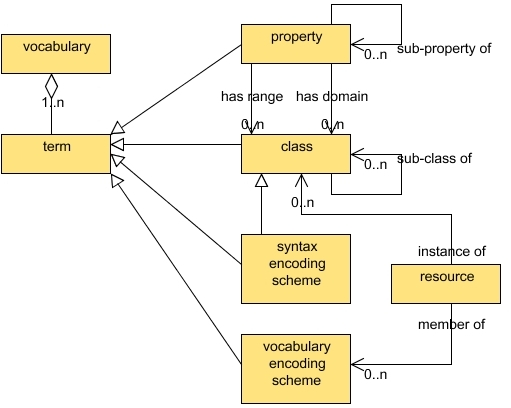
\includegraphics[width=0.6\textwidth]{images/vocabulary-model.jpg}
\caption{Modèle général du DCMI}
\label{img:dcmi-voc}
\end{figure}

\paragraph{Modèle général et représentation}
Une des grandes avancées de \pc{DCMI Metadata Terms}, a été la constitution d'une modélisation générale, voir la Figure \ref{img:dcmi-voc}, et l'introduction d'une syntaxe de représentation utilisants XML, RDF et RDF-S. 
En plus des propriétés, le modèle définit la notion de Classe et de Schéma d'encodage (qui sera expliqué ci-après). 
Les classes permettent de définir des types de ressources et de leur attribuer des URI. 

Chaque \pc{Terme} est défini par une liste d'attributs lui donnant un identifiant, une étiquette, une définition, ajoutant des commentaires, de la documentation, une référence complémentaire, les relations hiérarchiques avec les autres Termes, la classe et le type du Terme, l'appartenance à un Schéma d'encodage, les restrictions de sujet et d'objet qui s'applique à une propriété, les propriétés équivalentes.
Ainsi, on peut maintenant utiliser des URI, faisant référence à d'autres ressources, comme valeur d'une propriété.
Les valeurs peuvent donc être soit une expression littérale, une URI quelconque, ou bien une URI pointant vers un type de ressource particulier, comme un Terme appartenant à un schéma d'encodage ou une classe.
Par exemple, la propriété \pc{creator} ne peut pointer que vers des ressources de classe \pc{Agent} (du fait d'une restriction \pc{hasRange}). 


\paragraph{Schémas d'encodage}
Il existe deux types de schémas d'encodage qui permettent de préciser si les valeurs des propriétés sont écrites selon une syntaxe particulière (\pc{Syntax Encoding Scheme}, SES), ou si la valeur fait partie d'un thésaurus ou d'un vocabulaire contrôlé (\pc{Vocabulary Encoding Scheme}, VES).
Cela permet par exemple, d'indiquer que les valeurs de la propriété \pc{date} sont écrites suivant le format du W3C Date Time Format ou bien suivant la norme ISO 8106. 
De même, on peut déclarer que les valeurs de la propriété \pc{subject} seront prises dans la liste des \pc{Library of Congress Subject Headings}. 
%need REF ! 
SES et VES offrent ainsi la possibilité d'utiliser plusieurs jargons ou syntaxes pour caractériser les valeurs des propriétés, voir [A1] dans les besoins de modélisations du chapitre précédent (\ref{sec:bm}).
De plus, la spécification d'un Terme permet d'ajouter une définition et de pointer vers d'autres ressources pour documenter les Termes, voir [A2].

\begin{figure}[ht!]
\centering
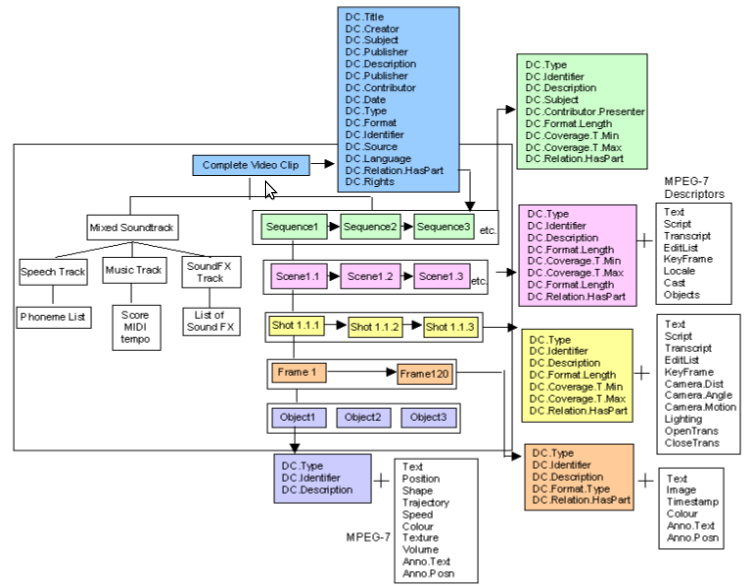
\includegraphics[width=0.8\textwidth]{images/HunterDCMI-MPEG7.png}
\caption{Modèle de Dublin Core étendu pour l'audiovisuel avec des descripteurs MPEG-7 (\cite{Hunter1999})}
\label{img:dcmi-mpeg7}
\end{figure}


\paragraph{Application à l'audiovisuel}
La modélisation du DCMI Metadata Terms s'intéresse à la description de tout type de ressources sur le Web (ce qui est identifié par une URI \cite{Berners-Lee1998}).
Cette perspective très générique lui permet de s'appliquer à de nombreux cas d'usages sans pour autant traiter leurs spécificités. 
Ainsi, dans le cas de l'audiovisuel il faudrait étendre ce schéma pour décrire par exemple le format d'image, les différents contributeurs, inclure de nouveaux types de dates, de nouvelles classes de Termes etc.

\cite{Hunter1998} ont proposé une extension qui raffine les propriétés du Dublin Core et les applique à différents niveaux de composition de l'objet audiovisuel, voire la Figure \ref{img:dcmi-mpeg7}.
Ainsi, l'objet audiovisuel est d'abord décomposé en élément audio (avec des pistes de paroles, de musique et d'effets) et vidéo.
Puis la vidéo est hiérarchisée en séquences, scènes, plans, images et objets dans une image.
À chaque niveau s'applique un ensemble de propriétés, dont des ajouts par rapport au schéma (la Description est lié à une liste de Genre, le Format permet d'indiquer le diffuseur).
\cite{Hunter1999} poursuivent ce travail et propose une représentation de ce schéma pouvant être intégré à MPEG-7. 


\paragraph{Discussion}
L'approche poursuivie par \cite{Hunter1999} est cependant assez contraignante du fait de la décomposition hiérarchique figée et non applicable à tous les types de production audiovisuelle.
En particulier, la notion de séquence et de scène est propre à la production de fiction. 
Les niveaux de hiérarchisation devraient s'adapter aux particularités de chaque type de production. 
De plus, la description des niveaux de fragmentation inférieurs à la séquence repose de plus en plus sur des descripteurs de MPEG-7. 
En effet, le nombre de propriétés de Dublin Core utilisées baisse à chaque niveau de fragmention et on n'utilise plus que trois propriétés pour le dernier niveau (\e{identifier}, \e{type} et \e{description} pour associer les descripteurs MPEG-7).
Ce déséquilibre progressif entre les deux schémas reflète bien leur cadre d'usage. 
Si Dublin Core est particulièrement pertinent pour les niveaux documentaires les plus hauts, sa pertinence diminue quand on rentre dans le détails des fragments audiovisuels.
Il est alors nécessaire de lui adjoindre un schéma de description propre à l'audiovisuel comme MPEG-7.
Finalement, un schéma comme DMS-1 (voir \ref{sec:wrapper}) apparaît comme plus adapté qu'une extension de Dublin Core + MPEG-7 pour couvrir ces besoins.
Et ce, d'autant plus, que DMS-1 fournit des informations plus adaptées à l'audiovisuel (ne serait-ce que l'exemple des titres) et favorise un découpage factuel extensible ainsi qu'une description éditoriale.



%=============
\subsection{MPEG-7 Part 5: Multimedia Description Scheme}\label{sec:mpeg7}
% \cite{Hunter2001} ; \cite{Troncy2007} ; \cite{Nack2005a} ; \cite{Dasiopoulou2009} ; \cite{Garcia2005} ; 

% à revoir
Parmi les normes utilisés pour décrire le contenu des audiovisuels, MPEG-7 est certainement devenu le standard de l'industrie. 
Développé à partir de 1998 par le comité MPEG (Moving Picture Expert Group) à la suite des standards MPEG-1, MPEG-2 (norme de compression du signal audiovisuel) et MPEG-4 (norme de d'encodage multimédia basée sur les objets), MPEG-7 est devenu une norme ISO/IEC en 2001 puis mise à jour jusqu'en 2006. 

La norme définit un ensemble de \e{Descripteurs} (Descriptors, Ds) dont les valeurs permettent de caractériser un objet audiovisuel, qu'il s'agisse de composantes du signal ou bien d'autres aspects comme des informations relatives à sa création, sa structure, son usage passé et futurs etc.
Ces Descripteurs sont organisés en \e{Schémas de Descriptions} (Description Schemas, DSs) dont on peut avoir une vue d'ensemble dans la Figure \ref{img:soa:mds}.
C'est cette partie de la norme (\cite[Part 5 : Multimedia Description Scheme]{ISO/IEC2003}) que nous traiterons en particulier dans cette section. 

\begin{figure}[ht!]
\centering
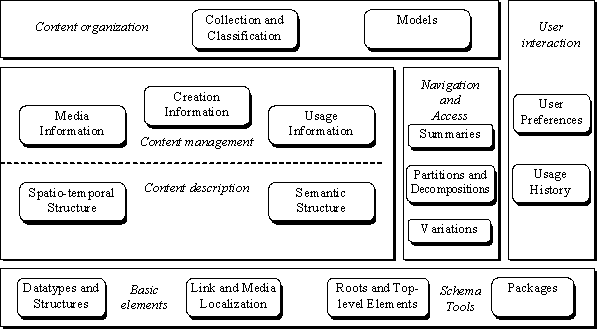
\includegraphics[width=0.8\textwidth]{images/MPEG-7-MDS.png}
\caption{Vue d'ensemble des Schémas de Description (DSs) de la norme MPEG-7}
\label{img:soa:mds}
\end{figure}

Les descriptions produites sont représentées dans un \e{Langage de Description des Définitions} (Description Definition Language, DLL) qui permet de spécifier la syntaxe des Descripteurs, la structure des Schémas de Description ainsi que la sémantique de l'ensemble.
Ce langage permet également de créer ou modifier des Descripteurs, d'étendre ou de modifier les Schémas de Descriptions. 
Le DLL est en réalité XML Schema (\cite{Fallside2004}) agrémenté de quelques types primitifs.

Pour utiliser MPEG-7, il faut également des outils et des directives annexes qui permettent de guider les utilisateurs. 
% définition / implémentation ? 
Dans la partie \e{Systems} de la norme, on trouve ainsi la définition d'outils qui remplissent les fonctions suivantes : codage d'une description MPEG-7 en binaire ; mécanismes de transmissions des descriptions (en binaire ou en texte) à part ou en parallèle du contenu audiovisuel décrit ;  synchronisation entre description et contenu audiovisuel ; gestion des descriptions et de la propriété intellectuelle. 
La partie \e{Reference Software} présente des logiciels de références pour utiliser la norme.
Enfin, la partie \e{Conformance} explicite des directives et des procédures pour s'assurer de la conformité des descriptions produites.

Nous détaillerons dans cette section les Schémas de Description liés à la gestion du contenu (\e{Content Management} dans la Figure \ref{img:soa:mds}) et à la description du contenu (\e{Content Description}).\\


\subsubsection{Gestion du contenu}
MPEG-7 définit trois concepts fondamentaux pour modéliser l'enregistrement d'une réalité en un contenu multimédia et les multiples transformations qu'il est possible de lui appliquer. 
Ainsi, pour chaque modalité d'enregistrement (audio, audiovisuel, photo etc.) MPEG-7 considère la création de trois éléments, une \pc{ContentEntity} (entité de contenu, CE), une \pc{MediaInstance} (instance de média, MI) et un \pc{MediaProfile} (profil de média, MP), voir la Figure \ref{img:soa:media}.
Pour donner une première idée, on peut dire que le fichier créé correspond à la \pc{MediaInstance}, que le \pc{MediaProfile} correspond aux paramétrages de son encodage et que la \pc{ContentEntity} représente le contenu de manière abstraite.

\begin{figure}[ht!]
\centering
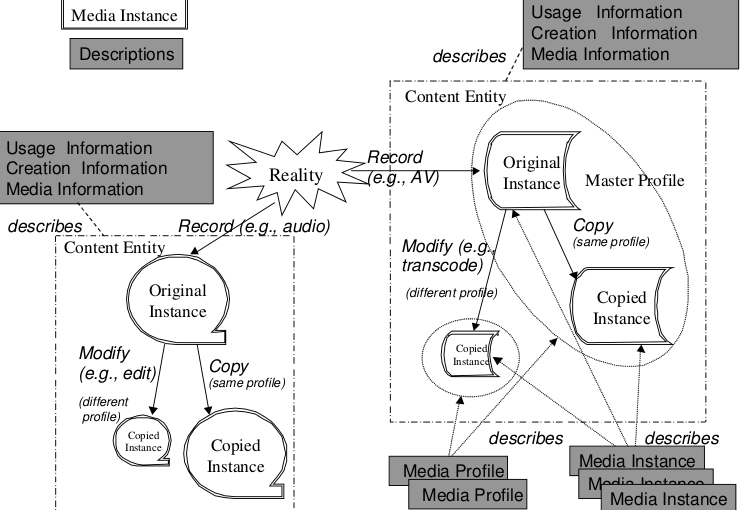
\includegraphics[width=0.8\textwidth]{images/MPEG-7-MediaManagement.png}
\caption{Gestion des contenus dans MPEG-7 à trois niveaux : contenu, instance et profile.}
\label{img:soa:media}
\end{figure}


On remarque qu'il existe cependant des différences entre les \pc{MediaInstance}, entre l'original et ce qui est nommé des \gui{copies} (copied instances). 
Ce qui est particulièrement intéressant pour nous est de constater que la nature de la manipulation entre l'original et les soi-disantes \gui{copies} importe peu (copie technique, réencodage ou montage), car cela crée de toute façon une nouvelle \pc{MediaInstance}. 

À l'inverse, la notion de \pc{MediaProfile} est dépendante de la nature de ces transformations. 
Le \gui{MasterProfile} correspond ainsi aux paramètres d'encodage de la MI d'origine, la première créée. 
Ainsi, dès qu'une différence d'encodage apparaît avec les MI créées ultérieurement, un nouveau \pc{MediaProfile} est créé. 
Il correspond donc à un regroupement de toutes les instances ayant en commun le même encodage. 
%%%% orthographe %%%%
Ce qui paraît troublant néanmoins, est l'amalgame fait entre réencodage et montage. 
Les changements de structure réalisés par le montage semblent en effet bien plus significatif qu'un changement de paramètre d'enregistrement. 
On peut se souvenir de la citation d'\pc{Eisenstein} à ce sujet évoqué en section \ref{sec:prod}.

Enfin, la notion de \pc{ContentEntity} correspond à une entité abstraite permettant de regrouper toutes les versions ultérieures de ce même contenu.
De ce fait, c'est à elle qu'on attache des informations concernant la création, l'usage et le type de média construit. % ??? Sûr ???
Ce regroupement d'informations à ce niveau découle de l'idée que chaque \pc{ContentEntity} définit une forme reconnaissable de contenu, quelque soit les variations apportées.
Encore une fois, l'idée qu'un montage différent n'impacte pas la forme et donc potentiellement l'identité du contenu nous semble ambiguë. 
Il s'agit là d'un de nos points d'achoppement par rapport à la modélisation proposée par la norme. 

\paragraph{Schémas de description}
Détaillons maintenant les trois Schémas de Descriptions proposés par MPEG-7 dans la partie \gui{Content Management}.
Remarquons que ces schémas s'appliquent tous à décrire les \pc{ContentEntity}.
% plus de détails sur les DSs

Le \pc{MediaInformation} est un schéma qui comporte des informations d'identification du CE ainsi qu'un ou plusieurs Profiles d'instances. 
Il faut remarquer que la définition du Profile proposé implique que le moindre changement d'encodage aboutit à la création d'un nouveau Profile en plus de l'instance. 
Il devient alors clair qu'un Profile représente la description d'un groupe d'instances, dont il facilite la gestion.
\begin{liste}
	\item \pc{MediaIdentification} : propose un ou plusieurs identifiants pour le CE.
	\item \pc{MediaProfile} : est composé de plusieurs descripteurs qui détaillent les paramètres et formats utilisés pour encoder une ou plusieurs instances.
	Il s'agit en particulier du \pc{MediaFormat} (pour l'encodage et le format d'encapsulation des données) ; le \pc{MediaInstance} (visant à identifier et localiser les instances) ; le \pc{MediaTranscodingHints} (pour faciliter le réencodage des données) ; le \pc{MediaQuality} (pour détailler la qualité et les défauts). 
\end{liste}


Le \pc{CreationInformation} peut être considéré comme une version étendue à l'audiovisuel des éléments du DCMI. Il comporte les Schémas de Description suivants : 
	\begin{liste}
		\item \pc{Creation} : des métadonnées qui permettent d'identifier le contenu (titre), proposer un résumé et des informations sur les conditions de sa création (créateur et contributeurs avec leur rôle, lieu, date, matériel et paramètrage utilisé).

		\item \pc{Classification} : des éléments de classification du contenu par forme (film, journal télévisé etc.), genre (sport, politique etc.), sujet, langage présent, et des informations sur la diffusion (date, région, public cible, critiques etc.)

		\item \pc{RelatedMaterial} : des métadonnées sur les autres versions d'un même contenu (format, type de média, localisation du média etc.) qui sont ensuite elles-mêmes décrites comme des éléments à part.
	\end{liste}

Le \pc{UsageDescription} est un schéma qui comporte un descripteur détaillant les droits attachés au contenu (\pc{Rights}), un descripteur décrivant les résultats financiers (\pc{FinancialResults}) et des schémas de descriptions sur les détails d'utilisation du contenu (\pc{Availability}) et sur l'historique de son utilisation(\pc{UsageRecord}).
Les droits d'exploitation peuvent en effet porter uniquement sur certains types de distribution (DVD, télédiffusion etc.) ou une certaine période. 
L'historique permet de garder trace des diffusions et de leur audience.


\subsubsection{Description du contenu}
\paragraph{La structure spatio-temporelle du contenu}
MPEG-7 fournit un ensemble de schémas et de descripteurs qui permettent de découper les contenus multimédias de toute les manières possibles. 
Pour cela, la norme définit la notion de \pc{Segment} qui se décline en segment spatial, temporel ou spatio-temporel et sur tout type de média (audio, image, audiovisuel, multimédia). 
Chaque segment peut se décomposer en d'autres segments suivant la structure d'un arbre. 
De plus, ces segments peuvent être connectés entre eux ou pas, c'est-à-dire spécifier trois zones connexes ou pas d'une image ou bien trois séquences temporelles qui se suivent ou pas. 
Les Segments peuvent également n'être valable que pour une source média particulière, comme une piste audio comportant la musique.

Un point particulièrement important est que chacun de ces \pc{Segment} est considéré comme une \pc{ContentEntity}. 
On peut donc utiliser les schémas de \pc{MediaInformation}, \pc{CreationInformation} et de \pc{UsageDescription} pour les décrire ainsi qu'un schéma \pc{Semantic} que nous décrivons ci-après. 
En plus de cela, de nombreux schémas spécifiques à la nature du média existent pour décrire le signal de manière analytique. 


\paragraph{Aspects sémantiques}
Le schéma \pc{Semantic} permet de décrire le monde qui est présenté aux lecteurs dans le contenu audiovisuel. 
Il s'agit d'une description basée sur les évènements (\pc{Event}) ayant lieu à tel moment (\pc{SemanticTime}), à tel endroit (\pc{SemanticPlace}), et auxquels participent des objets (\pc{Object}) ou des agents (\pc{AgentObject}). 
La description peut être raffinée en utilisant des concepts (\pc{Concept}), en détaillant les attributs d'une entité (\pc{SemanticState}) ou bien les relations entre entités (\pc{SemanticRelation}).
À noter, que ces relations peuvent tout autant porté sur les évènements se déroulant dans le contenu (par exemple, l'agent A est bénéficiaire d'un évènement B) ou bien entre un contenu et des entités sémantiques (par exemple, l'image A est une référence à l'objet B).

% VariationDescription !!!!







%Core Ontology for MultiMedia
%=============
\subsection{Ontologies basées sur MPEG-7}\label{sec:mpeg7etc}
% \addcontentsline{toc}{subsubsection}{Core Ontology for MultiMedia}
MPEG-7 est une norme qui propose de nombreux descripteurs pour modéliser les objets audiovisuels.
La grande force de son approche est d'associer ces descripteurs à n'importe quelle séquence de contenu multimédia.
Cette richesse amène également une certaine difficulté dans l'appréhension de sa modélisation, tant la norme est étendue et complexe. 
De nombreux auteurs ont critiqué l'approche de représentation de la norme, notamment du fait de l'ambiguïté sémantique et syntaxique des descriptions produites (\cite{VanOssenbruggen2004, Nack2005a, Troncy2007, Dasiopoulou2009, Arndt2007}).

En effet, si l'utilisation des langages XML semblait légitime à l'époque, il en résulte un manque de formalisation qui complique les raisonnements et l'interopérabilité avec d'autres schémas de description (\cite{Nack2005a}).
De plus, la possibilité de créer plusieurs variantes syntaxiques valides pour représenter la même description rend difficile leur maintien et leur intéropérabilité, et ce même avec d'autres descriptions MPEG-7 (\cite{Arndt2007}).
Une approche formalisée sémantiquement aurait permis de réconcilier ces différentes variantes de représentation. 

Deux autres inconvénients mis en évidence par \cite{Nack2005a} sont la rigidité structurelle des descriptions et l'abscence de relations entre documents. 
La description d'un fragment de contenu ne peut se faire hors d'une structure de description d'un document entier. 
Une fois cette structure fixée, elle ne pourra plus être altérée, sous peine de la rendre incompatible avec les anciennes versions.
Les relations doivent également être contenu à l'intérieur d'une description d'un document.
De ce fait, créer une relation entre deux programmes obligent à créer un document de type collection contenant ces deux programmes.

MPEG-7 reste une source de référence et d'inspiration pour plusieurs série de travaux qui tentent de pallier ces défauts de représentation.
Leur approche consiste à proposer une formalisation sémantique d'une partie du standard avec pour objectif de relier ces descriptions à des ontologies de domaine.
\cite{Troncy2007} et \cite{Dasiopoulou2009} ont étudié plusieurs de ces travaux en vue de les comparer, voir la Table \ref{tab:ontos} pour une synthèse de leur comparaison. 
Dans la suite de la section, nous présentons chacun de ces travaux avant de faire le point sur leur stratégies respectives d'intégration à des ontologies de domaine.
Enfin, nous discutons des apports et des manques de ces ontologies par rapport aux besoins que nous avons exprimés en début de chapitre (\ref{sec:bm-av}).

Ces travaux se distinguent de plusieurs manières : 
\begin{liste}
	\item par l'étendue de leur reprise de \g{MPEG-7} (colonne éponyme).
	On remarquera en particulier que ces ontologies se concentrent sur les parties de décomposition structurelle des objets audiovisuels (Structure), et sur les descripteurs bas-niveau (Visual DS et Audio DS).
	\item l'ontologie générique à laquelle il se raccroche (colonne \g{Ontologie}) 
	\item la conceptualisation utilisée pour réaliser des alignements et des liens avec des ontologies de domaine (colonne \g{Intégration}) 
	\item le type et le domaine d'applications visés (colonne \g{Applications}) 
	\item le langage de représentation utilisé (RDF-S ou OWL) (colonne \g{Langage}) 
	\item le type de modélisation, modulaire (fond blanc) ou monolithique (fond gris).
\end{liste}

\begin{table}[htb!]
% \begin{center}   			{l p{61pt} p{60pt} p{130pt} r}
							% {l p{55pt} p{35pt} p{55pt} p{130pt} r}
\begin{tabularx}{\textwidth}{|l|p{61pt}|X|X|p{130pt}|r|}
\hline
	\g{Nom} & \g{MPEG-7} & \multicolumn{2}{c|}{\g{Ontologie}~|~\g{Intégration}} & \g{Application} & \g{Langage} \\ \hline\hline
	
	\rowcolor{lightgray}
	\pc{Harmony} &  Structure+ Visual & \multicolumn{2}{>{\columncolor{lightgray}}c|}{ABC} & analyse et annotation d'image dans le milieu médical & OWL Full \\ \hline
	
	\pc{aceMedia} & Structure+ Visual& \multicolumn{2}{c|}{DOLCE Lite+ AO} & analyse et annotation de match de tennis & RDF-S \\ \hline

	\pc{SmartWeb} &  Structure+ Visual & \multicolumn{2}{c|}{SmartSUMO} & analyse et annotation de vidéo de match de football & OWL \\ \hline

	\pc{Boemie} & Structure+ Visual+Audio & -- & Boemie & analyse, annotation et recherche de documents multimédia & OWL-DL  \\ \hline
	
	\pc{COMM} & Structure+ Visual & \multicolumn{2}{c|}{DOLCE} & gestion de documents multimédia pour l'industrie & OWL-DL \\ \hline

	\rowcolor{lightgray}
	\pc{Rhizomik} & MPEG-7 en entier & -- & Semantic DS & conversion MPEG-7 XML vers OWL & OWL-DL \\ \hline

	\pc{DS-MIRF} & MDS complet & -- & Semantic DS & conversion MPEG-7 XML vers OWL (football et formule 1) & OWL-DL \\ \hline
\end{tabularx}
\caption{Synthèse des ontologies basées sur MPEG-7}\label{tab:ontos}
% \end{center}
\end{table}



\paragraph{\pc{Harmony}}
\cite{Hunter1999} ont réalisé la première tentative de formalisation sémantique de MPEG-7. 
L'ontologie \pc{Harmony} était représentée initiallement en RDF-S puis en OWL Full, et suit de près la modélisation proposée par MPEG-7. 
Il en résulte les mêmes constats que pour MPEG-7, la modularité des descriptions ainsi qu'une ambiguïté syntaxique et sémantique.

Les travaux de \cite{Hunter2001} ont intégré l'ontologie générique ABC permettant de modéliser des temporalités (évènement, situation, action), des actualités (artefact ou agent) et des oeuvres.
L'intégration d'ABC doit aussi permettre de créer des relations ou des alignements avec des ontologies génériques ou de domaine, pour favoriser l'interopérabilité la spécialisation des descriptions. 
\cite{Hunter2004} est un exemple d'utilisation de l'ontologie pour l'annotation et l'analyse d'images médicales. 


\paragraph{\pc{aceMedia}}
Le projet \pc{aceMedia}\footnote{http://www.acemedia.org} a développé deux ontologies basées sur MPEG-7. 
La \pc{Multimedia Structure Ontology} (MSO) pour la description de la structure des objets audiovisuels, et la \pc{Visual Descriptor Ontology} (VDO) pour les aspects visuels (\cite{Petridis2004, Martinez2002}).
Ces ontologies proposent une modélisation modulaire, proche de MPEG-7, mais qui clarifie certaines ambiguïtés syntaxiques, à l'inverse d'\pc{Harmony}.
Par exemple, MSO introduit les classes \cd{mso:Frame} et \cd{mso:KeyFrame} afin de distinguer leur rôle respectif. 
Dans MPEG-7 et \pc{Harmony}, la description d'une image pouvait résulter de l'utilisation d'un \pc{VideoSegment} ou d'une \pc{StillRegion}.

MSO et VSO utilisent deux ontologies génériques, DOLCE Lite et l'Annotation Ontology (AO).
L'AO a été construite pour spécialiser les entités de DOLCE (\cite{Borgo2002}) afin de faciliter la mise en relation avec des ontologies de domaine.
Ces ontologies ont été utilisé pour l'analyse et l'annotation d'images et de vidéos dans le domaine du sport (jeu de tennis, \cite{Petridis2006}) et pour des vidéos personnelles.


\paragraph{\pc{SmartWeb}}
Le projet \pc{SmartWeb}\footnote{http://www.smartweb-projekt.de/start\_en.html} a permis de développer un ensemble d'ontologies pour construire des services d'in\-fo\-rmation sur le Web. 
Parmi cet ensemble, on trouve une ontologie d'annotation de contenu multimédia qui se construit sur l'ontologie générique SmartSUMO (\cite{Oberle2007, Vembu2006}).
SmartSUMO est elle-même développée dans ce projet à partir de DOLCE (\cite{Borgo2002}) et SUMO (\cite{Niles2001}). 
Par rapport aux deux premières ontologies, celle-ci permet d'ajouter des informations de création et de production en formalisant le processus d'annotation lui-même.

Une particularité de la modélisation est de considérer les objets multimédia et les segments comme deux classes soeurs, et non comme une spécialisation, ce qui amène certaines ambiguïtés dans des décompositions complexes.
L'ontologie a été utilisée pour l'analyse et l'annotation de vidéos de match de football.


\paragraph{\pc{Boemie}}
Le projet \pc{Boemie}\footnote{http://www.boemie.org/} a permis de développer deux ontologies ; la \pc{Multimedia Content Ontology} (MCO) et la \pc{Multimedia Descriptors Ontology} (MDO). 
Ces ontologies visent à re-modéliser MPEG-7 en OWL-DL, du point de vue de la décomposition des objets audiovisuels et des descripteurs audio et vidéo de bas-niveau (\cite{Dasiopoulou2009a}).

On retrouve la séparation entre objets audiovisuels et segments, mais cette modélisation utilise des restrictions de classes pour éviter toute ambiguïté.
La décomposition peut également se faire de manière indépendante sur un plan logique (unité logique) et factuel (segments).
Le lien avec des ontologies de domaine se fait par des relations pointant vers des concepts génériques de MCO.
\cite{Karkaletsis2005} proposent une utilisation de ces ontologies dans le cadre de l'analyse, l'annotation et la recherche de documents multimédia.


\paragraph{COMM}
La \pc{Core Ontology for MultiMedia} (COMM) est la tentative la plus récente de formalisation de MPEG-7 (\cite{Arndt2007, Staab2008, Arndt2009}).
Ce travail permet de spécialiser au domaine de l'audiovisuel les patrons de conception (Design Pattern) suivants : \pc{Descriptions \& Situations} (D\&S) et \pc{Ontology of Information Objects} (OIO) de DOLCE (\cite{Gangemi2005}).
COMM retravaille la modélisation de MPEG-7 pour la formaliser et la rendre modulaire. 

COMM définit 4 patrons ; la \e{décomposition structurelle} d'un objet en segments multimédia ; l'\e{annotation de contenu} qui permet d'associer des informations à un objet ou un segment ; l'\e{annotation du média} qui décrit les fichiers multimédias, leur encodage etc. ; l'\e{annotation sémantique} qui permet d'associer les objets ou segments multimédias avec des éléments d'ontologies de domaine. 
Une des particularités de COMM est de formaliser le processus d'annotation, mais pas tout à fait de la même manière que les ontologies de \pc{SmartWeb}.
L'annotation est ici le résultat d'une méthode d'annotation (manuelle, automatique), dont on peut décrire les paramètres, et qui sert de lien entre l'élément annoté et l'annotation sémantique.

L'ontolgoie COMM a été utilisée pour la gestion de documents multimédia dans des applications industrielles (comparateur de voitures, gestion de problèmes moteur pour l'aéronautique).
Si COMM clarifie la modélisation de MPEG-7, l'utilisation de DOLCE tend également à la complexifier.
Ainsi, une API\footnote{http://multimedia.semanticweb.org/COMM/api} Java a été développée pour cacher cette complexité et faciliter la création de descriptions et l'implémentation de services de recherche.



\paragraph{\pc{Rhizomik}}
Contrairement aux approches précédentes, \cite{Garcia2005} ont developpé une méthode de conversion automatique de MPEG-7 dans le cadre du projet \pc{ReDeFer}\footnote{http://rhizomik.net/redefer}.
Alors que les autres approches retravaillent la modélisation de MPEG-7 pour la clarifier et l'ajuster à leurs besoins, cette méthode reprend directement le XML Schema du standard.
La méthode repose sur deux langages d'alignement, XML2RDF et XML2OWL qui permettent de convertir tous les éléments en une ontologie OWL nommée \pc{Rhizomik}.

La séparation entre objets et segments multimédia est totale puisque les deux classes ne sont même pas soeurs.
De plus, reprenant MPEG-7, cette nouvelle représentation conserve les défauts déjà mentionnés : ambiguïté et complexité.
Du point de vue de la mise en relation avec des ontologies de domaine, cela est rendu possible par l'intermédiaire du Semantic DS.
Cette modélisation (décrite en \ref{sec:mpeg7}) est plus orienté et moins complète que celle proposée par des ontologies génériques.
De plus, l'approche nécessite d'utiliser un XML Schema pour définir les concepts du domaine, avant de pouvoir effectuer la transformation en une ontologie OWL.
De ce fait, l'ontologie est mieux utilisée pour transformer des descriptions MPEG-7 que pour faciliter l'intégration avec d'autres ontologies.


\paragraph{DS-MIRF}
\cite{Tsinaraki2004a, Tsinaraki2007} présentent le DS-MIRF framework qui traduit manuellement le MDS, l'Audio DS et le Visual DS en une ontologie OWL-DL.
Plus précisément, la transformation est pilotée par une ontologie tierce qui définit les alignements en le XML Schema et les entités OWL.
Cette méthode permet d'expliciter et de clarifier certaines ambiguïtés de MPEG-7, mais la structure de l'ontologie reste proche de celle de \pc{Rhizomik}.

Une méthodologie a été proposée pour traduire systématiquement les déclarations réalisées avec une ontologie de domaine en déclarations compatibles avec la sémantique de MPEG-7.
Ainsi, contraiment à la méthode de \pc{Rhizomik}, l'intégration avec d'autres ontologies est réalisé en définissant un alignement, plutôt qu'en transformant les ontologies en XML Schema.
Le DS-MIRF framework a été utilisé pour l'annotation de match de football et de courses de Formule 1.


\paragraph{Stratégies d'intégration à des ontologies de domaine}
En guise de synthèse, nous comparons les stratégies d'intégration des ontologies basées sur MPEG-7 avec des ontologies de domaine.
Ces ontologies de domaine servent à produire des descriptions sur le contenu d'objets ou segments multimédia, en proposant des concepts et des propriétés spécifiques à ce domaine. 
Nous avons vu que de nombreux exemples d'applications s'intéressent à un domaine sportif (football, tennis etc.).
Cela permet alors d'enrichir la description, essentiellement techniques, de ces objets et de proposer une indexation propre à un métier.
Les ontologies présentées mobilisent trois stratégies : 
\begin{liste}
	\item \e{l'utilisation d'une ontologie générique} pour faire le lien entre les objets multimédias et des descriptions issues de l'ontologie de domaine. 
	C'est le cas de l'ontologie \pc{Harmony} avec ABC, des ontologies du projet \pc{aceMedia} et \pc{Boemie}.
	L'ontologie générique fournit des classes génériques que l'ontologie multimédia et de domaine peuvent spécialiser. 
	Ces classes sont reliées par des propriétés génériques, et spécialisables, qui permettent de relier un objet multimédia avec des déclarations de l'ontologie de domaine.
	Dans ce cas, l'intégration entre les ontologies dépend fortement de l'architecture de l'ontologie générique.

	\item \e{l'utilisation du Semantic DS}, moins complet et plus orienté que les ontologies génériques.
	C'est le cas des ontologies \pc{Rhizomik} et DS-MIRF, même si elles n'utilisent pas tout à fait la même méthodologie (voir leur présentation) pour faire l'intégration.

	\item \e{une formalisation de la méthode de création des liens} en plus de la formalisation des liens entre objets multimédia et descriptions sémantiques. 
	C'est l'approche utilisée dans COMM et les ontologies de \pc{SmartWeb}.
\end{liste}

Enfin, il est important de noter que dans les approches utilisant des ontologies génériques, la modélisation des objets audiovisuels est indépendante de la stratégie d'intégration à des ontologies de domaine. 
Ainsi, il serait possible d'utiliser la dernière approche dans \pc{Harmony}.

\paragraph{Discussion}
[\g{B1 : autonomie}]
[\g{B2 : réutilisabilité}]
%  structure documentaire générique, extensible ?
%  description propre à la prod. av ? le signal tend mais n'y est pas encore
% intégration avec des ontos de domaine importante, bcp d'efforts pour des formalismes de haut-niveau, mais du coup difficile à appréhender par les utilisateurs, problème d'adoption ?
% peu de lien avec le contexte, approche a posteriori qui ne permet pas de prescription ou de description au fil de la production




%=============
\subsection{Ontology for Media Resources}
Suite aux travaux du W3C Media Annotation Working Group (MAWG), \cite{Burger2011} puis \cite{Lee2012} ont développé une ontologie minimaliste pour décrire et rechercher des informations sur des ressources média sur le Web.

\begin{figure}[ht!]
\centering
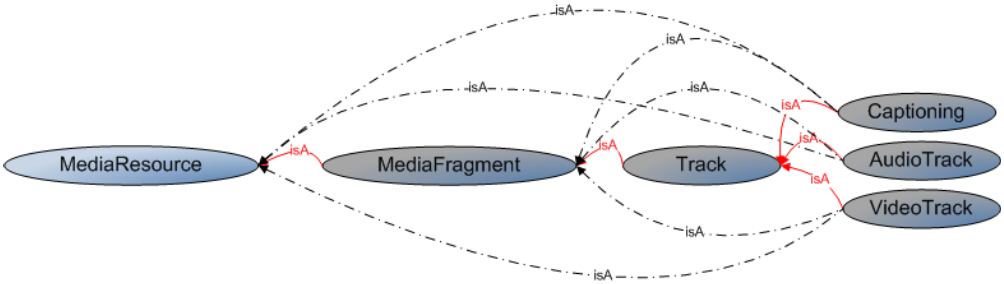
\includegraphics[width=0.8\textwidth]{images/MA-model.png}
\caption{Hiérarchie de classes sous le concept de \pc{MediaResource}}
\label{img:ma-model}
\end{figure}

La modélisation repose sur les concepts de \pc{Collection}, \pc{MediaResource}, \pc{MediaFragment}, \pc{Track} et \pc{Image}, voir la Figure \ref{img:ma-model}.
La décomposition des objets multimédia se fait donc par des fragments, que l'on peut ensuite décomposer en piste et en image.
Cette simplicité apparente, comparée aux approches de segmentation complexe de MPEG-7, cache en réalité l'utilisation d'une autre recommandation du W3C.
La définition d'un MediaFragments peut se faire à partir de l'URI de son média source, où l'on ajoute un syntaxe de décomposition (\cite{Hausenblas2011}).
Par exemple, l'url suivante \cd{http://www.example.com/example.ogv\#t=10,20} désigne le fragment temporel commençant à 10s. et finissant à 20s.
La décomposition peut se faire selon une dimension spatiale, temporelle, en pointant une piste de la source, en pointant un autre fragment prélablement identifié, ou bien n'importe quelle combinaison de ces dimensions.
Des informations techniques (encodage, durée, format etc.) peuvent également être associée aux ressources.

En plus de ces classes, on trouve dans l'ontologie le concept d'\pc{Agent} (personne ou organisation), de \pc{Location} (lieu), de \pc{Genre} (le genre de programme suivant un dictionnaire spécialisé), de \pc{Rating} (permettant d'enregistrer les évaluations de lecteurs/spectateurs) et de \pc{TargetAudience} (indiquant le public visé par la ressource).
Ces classes supplémentaires permettent d'ajouter des informations sur le contexte de création (qui a participé, où) et de faciliter la diffusion et la recherche de ressource (genre, note, public cible etc.).

\begin{figure}[ht!]
\centering
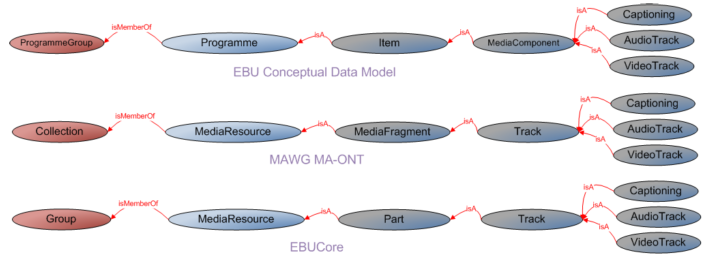
\includegraphics[width=\textwidth]{images/MA-alignement-A.png}
\caption{Alignement avec des ontologies multimédia (partie 1)}
\label{img:ma-alignement-A}
\end{figure}

\paragraph{Alignement avec d'autres conceptualisations}
Un apport important de cette ontologie réside dans le travail d'alignement avec les autres modélisations multimédia. 
Les Figures \ref{img:ma-alignement-A} et \ref{img:ma-alignement-B} présentent un alignement minimaliste des principales classes de l'\pc{Ontology for Media Resource}.
Dans la définition de \cite{Lee2012}, les alignements sont étendus à d'autres conceptualisations ainsi qu'aux propriétés de schémas de métadonnées et métadonnées embarquées dans des formats conteneurs.
Ainsi, on se rend compte que ces classes principales, qui représentent une collection d'objets multimédia, un objet, ses fragments et ses pistes de contenu, se retrouvent dans toutes ces modélisations. 
Les variations se situent à la fois dans la manière de découper/segmenter cet objet en fragment (dimension spatiale, temporelle etc.), de le lier aux média et dans la manière et la nature des informations que l'on peut leur associer.

\begin{figure}[ht!]
\centering
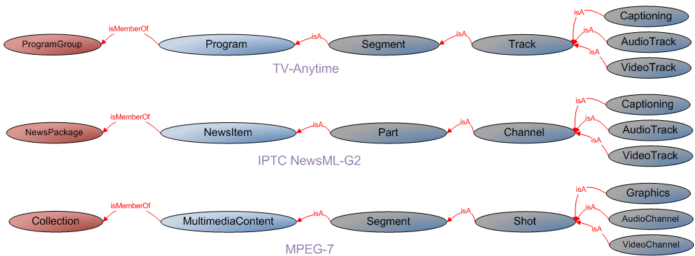
\includegraphics[width=\textwidth]{images/MA-alignement-B.png}
\caption{Alignement avec des ontologies multimédia (partie 2)}
\label{img:ma-alignement-B}
\end{figure}

\paragraph{Discussion}
L'\pc{Ontology for Media Resource} (OMR) a été construite dans un souci de clarté, de cohérence et d'extensibilité et s'intégre particulièrement bien avec les autres recommandations du W3C, dont le Media Fragment URI et SKOS.
L'objectif étant (1) de pouvoir publier des déclarations sur le web de données et (2) construire des systèmes de recherche de contenu interopérables. 
En effet, le travail réalisé sur les alignements permet d'extraire et traduire les informations contenues dans les dépôts n'utilisant pas les mêmes modèles.
Une API\footnote{http://www.w3.org/TR/2010/WD-mediaont-api-1.0-20100608/} a également été construite pour faciliter ces opérations et le déploiement de service de recherche et d'aggrégation de résultats provenant de ces différentes sources.

L'ontologie OMR ne se positionne donc pas comme un supplément de modélisation, mais plutôt comme un travail de synthèse et de mise en correspondance des travaux existants dans une représentation standardisée.
Son objectif n'est pas l'exhaustivité de la représentation des objets audiovisuels ou bien de leur description, mais bien de mettre en commun l'ensemble des informations dispersées et cloisonnées dans les dépôts.





%=============================
%=============================
\subsection{Descriptions métiers basées sur le plan}\label{sec:plan}
Script, Storyboard (\cite{Martin2005}, \cite{ThiBui2003}) etc.
Réappropriations dans le champ informatique : \cite{Chakravarthy2009b} ; \cite{Chakravarthy2009c}

Another trail of research has emerged recently. 
In comparison to the previous approach, it does not attack the multimedia description from below (with signal processing techniques) but from above. 
The principles is to represent the knowledge included in documents related to the multimedia content. 
It can be a web-page where the image is published and commented by others \cite{Simperl2009} or more specific documents related to the production context. 
\cite{Chakravarthy2009b} and \cite{Chakravarthy2009c} take interest in the knowledge of film direction. 
They propose a semantic model which captures the information typically included in a storyboard or screenplay. 
They also provide a system to capture the director's demands and assist her/him during the shooting. 
A similar work has been carried out by \cite{VanRijsselbergen2009} but with distinct goal and language. 
Their MovieScriptMarkupLanguage (MSML) captures the information of a shooting script with a particular attention to the details of set equipment's and actor's positions. 
The related Scoop system \cite{Cardinaels2008} provides its user 3D model of the set as well as the shots taken by the camera in a given position and settings. 
The overall objective is to provide an shooting-set 3D simulation to assist the production team in their preparation.\\





% Our approach follows this trend of research with different focus and objectives than the works presented. We consider the shooting script as the main production document to describe the video shots. The focus is on the realization of these shots, not the preparation or direction of the production. It does not assist the same people and do not provide exactly the same pieces of information. As we demonstrated above, a Semantic Script can assist the cameraman at shooting time and the professional editor when reviewing. 
% In comparison to the COMM ontology, our model offers an additional representation layer with describe the editorial structure of audiovisual objects (Opus, MediaAsset, EditorialObject). With the Semantic Script, we provide a way to predefine a structure and capture intentions that are inherent to the audiovisual production process. COMM represents a MPEG-7 flavored description of video files and also the way this description has been produced by human or algorithms. This indexing is made after the video production and do not provide any mean to retain information from the context of production.


\subsection{Discussion}
[\g{B1 : autonomie}]
[\g{B2 : réutilisabilité}]

%=============
\paragraph{MPEG-21}
% \addcontentsline{toc}{subsubsection}{MPEG-21}
% \cite{Burnett2003} ; \cite{Garcia2010} ? 
%Creation Value Chain
Along with MPEG-7, the MPEG-21 Multimedia Framework \cite{Burnett2003} offers a valuable perspective on future practices in content management, distribution and consumption. The recent interest in content value chains modeling presented in \cite{Garcia2010} shows some similarities with our audiovisual object modeling approach. There is still an open debate about the modeling of the various forms or facets that content can take during its production. Many approaches rely on, adapt or extend the original FRBR Group 1 concepts of \e{Work}, \e{Expression}, \e{Manifestation} and \e{Item}. 
For instance, the Media Value Chain Ontology (MVCO) \cite{Rodriguez-Doncel2009}, \cite{Rodriguez-Doncel2010} is included as the Part 19 of the MPEG-21 standard. 
The authors merge the concepts of Expression and Manifestation. Moreover, they also propose a new concept of Product for asset which needs to be licensed before publishing. 
% Citer également : Jane Hunter -- Reconciling MPEG-7 and MPEG-21 Semantics through a Common Event-Aware Metadata Model




%=============
\paragraph{TV Anytime}
% \addcontentsline{toc}{subsubsection}{TV Anytime}
\cite{Evain2000} ; \cite{Tsinaraki2004} ; \cite{Tsinaraki2005}



% % \cleardoublepage




% %%%%%%%%%%%%%%%%%%%%%%%%%%%%%%%%%%%%%%%%%%%%%%%%%%%%%%%%%%%%%%%%%%%%%%%%%%%%%%%%%%%%%%%%%%%%%%%%%%%
% %%%%%%%%%%%%%%%%%%%%%%%%%%%%%%%%%%%%%%%%%%%%%%%%%%%%%%%%%%%%%%%%%%%%%%%%%%%%%%%%%%%%%%%%%%%%%%%%%%%
\part*{Contribution}
\addcontentsline{toc}{part}{Contribution}
\chapter{Approche et modélisation}\label{chap:mod}

\e{
L'objectif de la partie \g{Contribution} est de présenter notre conceptualisation et sa représentation informatique dans le cadre plus général d'une approche de description des documents audiovisuels contributive et qui suit le déroulement de la production audiovisuelle, même dans des cas de réutilisation et de production collaborative impliquant des communautés de professionnels ou d'amateurs.
Ainsi, en plus des problèmes de modélisation de la diversité des documents audiovisuels, de leurs différents niveaux de représentation, s'ajoute des problèmes d'échange de connaissances entre contributeurs hétérogènes, qui ne partagent pas les mêmes conceptions, vocabulaires et compétences.
}

\e{
Nous commençons par résumer notre analyse des langages et modélisations étudiés dans les chapitres précédents (\ref{sec:synthese}) pour mettre en évidence les manques des solutions disponibles pour répondre aux problèmes soulevés. 
Cela nous amène à présenter les principes de notre approche qui met en avant la complémentarité des informations produites avant et après la fabrication du matériel audiovisuel (\ref{sec:approche}).
Nous introduisons également l'architecture développée dans le cadre du projet MediaMap pour opérationnaliser cette approche, et notamment les applications nécessaires à son fonctionnement.
Nous présentons en section \ref{sec:axes} une reformulation des verrous scientifiques que nous avons identifiés en section \ref{sec:scien}, ce qui nous permet d'introduire des patrons de conception pour représenter les situations typiques de \e{la} production audiovisuelle (\ref{sec:situations}).
% Ensuite, nous expliquons notre modélisation en introduisant des patrons de conception qui rassemblent les concepts et relations nécessaires à la représentation de situations typiques de la production audiovisuelle (\ref{sec:concept}).
Nous discutons ensuite de la mise en oeuvre de ces patrons (\ref{sec:meo}), qu'il s'agisse de les représenter dans un langage informatique, de donner des exemples d'instanciations ou de spécialisations ou encore de documenter le modèle afin de faciliter l'accès et l'échange des connaissances qu'il exprime.
}


\e{
Dans le chapitre \ref{chap:app}, nous présentons les applications développées par les partenaires du projet MediaMap (\ref{sec:app}) et les expérimentations qui ont été menées avec (\ref{sec:xp}).
Nous présentons finalement notre réflexion sur la validation de notre modélisation, notamment dans le cadre du projet MediaMap (\ref{sec:val}).
% Nous discutons également la représentation de notre conceptualisation avec le langage OWL, notamment en comparant certains de nos choix avec ceux effectués dans SKOS (\ref{sec:op}).
% Finalement, nous argumentons la validité de la modélisation de nos patrons de conception sur le plan informatique et sémantique (\ref{sec:val}).
}

\minitoc

%%%%%%%%%%%%%%%%%%%%%%%%%%%%%%%%%%%%%%%%%%%%%%%%%%%%%%%%%%%%%%%%%%%%%
%%%%%%%%%%%%%%%%%%%%%%%%%%%%%%%%%%%%%%%%%%%%%%%%%%%%%%%%%%%%%%%%%%%%%
%%%%%%%%%%%%%%%%%%%%%%%%%%%%%%%%%%%%%%%%%%%%%%%%%%%%%%%%%%%%%%%%%%%%%
\section{Synthèse de l'état de l'art}\label{sec:synthese}
Dans le chapitre \ref{chap:omod}, nous avons étudié la modélisation de connaissances par les ontologies ainsi que la modélisation des vocabulaires métiers par les terminologies. 
Notre définition des besoins implique d'associer une documentation et une terminologie à notre conceptualisation (\ref{sec:bm}), de manière à faciliter les échanges de connaissances entre tous les contributeurs de la chaîne de production, ainsi que dans les cas de réutilisation où l'on intègre des éléments externes dans sa chaîne.
L'analyse des langages documentaires (\ref{sec:xml}) et de représentation de connaissances (\ref{sec:onto-mc}) montre que leur conception les rend trop généraliste pour couvrir nos besoins spécifiques. 
Nous nous appuyons donc sur leur formalisme pour développer des principes de documentation, qui généralisent les propositions des langages de représentation de thésaurus et vocabulaire structuré (\ref{sec:thesaurus}) à la gestion des jargons métiers.
Ceci nous permet de couvrir nos besoins de représentation et de documentation du vocabulaire propre à la production audiovisuelle, et \e{in fine} d'adapter la forme d'expression des connaissances échangées entre contributeurs hétérogènes.

% Nos objectifs dépassent le cadre de la modélisation documentaire que permet XML et les langages de schéma associés (\ref{sec:xml}).
% Les langages de représentations des connaissances développés par le W3C apportent une formalisation qui permet de clarifier la sémantique de la modélisation et d'envisager la mise en place d'inférences (\ref{sec:onto-mc}).
% Si les langages RDF et RDF-Schema permettent la définition de hiérarchies de classes et de relations, OWL ajoute de nombreux raffinements dont de nouveaux axiomes précisant l'usage des propriétés, ainsi que l'ajout de propriétés d'annotation pour décrire la conceptualisation.
% La version OWL-DL fournit un compromis intéressant entre expressivité et décidabilité, mais ne permet pas de couvrir tous nos besoins [$\delta_1$ : \g{multijargon}].

% Ainsi, nous avons étudié les langages de représentation de thésaurus et vocabulaire structuré (\ref{sec:thesaurus}).
% SKOS et SKOS-XL proposent une représentation minimale et extensible des thésaurus existants, et apporte une formalisation qui permet leur publication sur le Web de données.
% La norme ISO-25964-1 apporte la composition des termes et proposent d'associer plus d'informations sur la création, la maintenance et la documentation du thésaurus.
% Les deux approches se concentrent sur la structuration des concepts auxquels on intègre (SKOS) ou on rattache des termes (dans SKOS-XL et ISO-25964-1, les termes sont définis indépendamment des concepts). 
% Cependant, cette indépendance n'offre pas la possibilité de grouper les termes entre eux afin de modéliser une terminologie métier [$\delta_3$ : \g{évolution, gestion}]. 
% De même, ces modèles définissent des termes préférés qui visent à normaliser l'usage linguistique d'une communauté métier, quelque soit la langue parlée par ses membres.
% Les différences d'usages entre métiers, organisation ou bien entre amateurs et professionnels ne sont pas représentées [$\delta_1$ : \g{multi-jargon}]. 
% La documentation des concepts et des termes correspond tout à fait à nos besoins, en particulier dans SKOS avec la notion de note qui permet de s'adapter à la spécificité de chaque usage [$\delta_2$ : \g{documentation}].\\



Dans le chapitre \ref{chap:mav}, nous avons étudié la manière dont les objets audiovisuels (\ref{sec:dav}) et leur réutilisation (\ref{sec:gest}) étaient envisagées dans différentes communautés.
Il se dégage de cette étude un point de vue centré sur le matériel audiovisuel (le signal) et un autre, documentaire, qui considère l'objet comme une articulation de différentes formes matérielles et sémiotiques. 
Cette approche considère ainsi non pas un objet, mais un document qui prend part à un acte de communication, et dont chacune des dimensions joue un rôle précis. 
% Nous avons mis en avant des divergences et des points aveugles entre les points de vue des professionnels de la production et des communautés scientifiques du multimédia, de l'ingénierie documentaire, de la sémiotique audiovisuelle et des bibliothèques numériques.

Nous nous sommes ensuite intéressés tour à tour à l'étude des formats conteneurs (\ref{sec:wrapper}) et d'autres modélisations des objets audiovisuels.
Le succès des formats conteneurs montre l'importance de l'association d'informations métiers au matériel audiovisuel, pour le déroulement de la chaîne, et l'exploitation de document audiovisuel.
Cependant, on remarque que le format de représentation de ces informations pose un problème d'ambiguïté sémantique et qu'il ne peut être utilisé en début de chaîne, avant la fabrication du matériel.
% L'étude des formats conteneurs nous a montré qu'il était possible de modéliser les objets audiovisuels suivant les perspectives administratives, narratives et documentaires tout en y intégrant le matériel audiovisuel [$\chi_1$ :\g{autonomie}]. 
% Cependant, cette forte intégration ne peut être mise en place qu'à partir de la fabrication du matériel, et vise pas au-délà de sa diffusion.
% De même, l'utilisation d'un format conteneur façonne la modélisation autour de l'objet audiovisuel final, et même s'il embarque des métadonnées sur les fragments, elles ne peuvent être mobilisées pour elle-même.
% Ainsi, la nature même du format oblitère le début de la chaîne et ne permet pas de se concentrer sur des fragments.
% Par ailleurs, nous avons pointé l'ambiguïté sémantique des descriptions associées au matériel audiovisuel [$\chi_2$ :\g{réutilisabilité}].

% \e{
% 	Les formats conteneurs ont montré l'importance de certaines informations pour le déroulement de la chaîne, et l'exploitation de document audiovisuel.
% 	Notre modélisation s'inspire de cette approche et vise à l'améliorer sur les aspects suivants : 
% 	\begin{liste}
% 		\item La modélisation des connaissances associées au document audiovisuel doit pouvoir débuter en début de chaîne, avant même la fabrication du matériel audiovisuel.
% 		\item La modélisation du document audiovisuel et des connaissances associées doit être formalisée pour éviter les ambiguïtés sémantiques ainsi que les problèmes d'appropriation de la part des contributeurs de la chaîne de production.
% 	\end{liste}
% }

Nous avons ensuite examiné des modélisations de l'audiovisuel que l'on a distinguées en deux approches, \e{endogène} et \e{exogène}, que nous jugeons complémentaires. 
Ces approches mettent l'accent respectivement sur la dimension sémiotique ou matérielle des objets audiovisuels (\ref{sec:dav}) sans vraiment les articuler.
% La modélisation \e{endogène} rend compte des connaissances fabriquées en début de chaîne afin de prévoir les étapes suivantes de fabrication du document et du matériel audiovisuel (\ref{sec:insitu}).
% Ces modélisations se rapprochent d'une modélisation documentaire du script, définissant la structure documentaire auctoriale (\ref{sec:pv-id}) et les intentions de mise en forme.
% Cette modélisation du script repose sur une unité de base qui est le plan (introduit dans ce mémoire en \ref{sec:docvoc}).
% Ce découpage est particulièrement intéressant du fait que le plan est à la fois l'élément de base de la narration audiovisuelle (structure documentaire) et l'unité de travail dans le processus de production (description de la fabrication, lien avec le matériel audiovisuel). 
% Il permet ainsi d'associer de multiples connaissances à des fragments audiovisuels. %et facilite ainsi leur réutilisation [$\chi_2$ : \g{réutilisabilité}].
% Le modèle MSML se limite à une représentation XML du script utilisé pour construire une prévisualisation 3D du plateau de tournage ainsi que du résultat filmé (\ref{sec:msml}). 
% Le manque de formalisation sémantique ne favorise pas la transformation de ces informations et leur association avec le matériel audiovisuel effectivement fabriqué [$\chi_1$ : \g{autonomie}].
% L'autre modèle étudié propose une formalisation sémantique ainsi qu'une association entre une description du document et du matériel audiovisuel (\ref{sec:answer}).
% Cependant, ces travaux ne sont pas accessibles et ne peuvent donc être repris ni évalués.
% 
% Les approches \e{exogènes} (\ref{sec:post}) proposent d'analyser le matériel audiovisuel en fin de chaîne. 
% L'approche générique du schéma Dublin Core, même lorsqu'il est spécialisé pour les documents audiovisuels, est surtout pertinente au niveau du document (\ref{sec:dcmi}). 
% La description des fragments n'est ainsi rendue possible que par l'utilisation de descripteurs spécifiques, comme ceux de la norme MPEG-7. 
% De plus, on remarque l'importance d'une structure hiérarchique souple et extensible qui permet de couvrir les nombreux genres de documents produits par la télévision.
% MPEG-7 s'est établie comme une modélisation de référence pour l'audiovisuel (\ref{sec:mpeg7}).
% Pourtant, sa représentation en XML a été largement critiquée pour son ambiguïté syntaxique et sémantique qui a poussé de nombreux chercheurs à développer des formalisations sous la forme d'ontologie (\ref{sec:mpeg7etc}).
% Ces modélisation sont réalisées de manière automatique ou manuelle, et certaines reposent sur une ontologie générique pour favoriser l'intégration avec des ontologies de domaine.
% Au-délà de ces apports, les modèles, comme la norme MPEG-7, adopte un point de vue centré sur le matériel audiovisuel tant au niveau de la gestion que de la description des objets audiovisuels. 
% Ainsi, ils négligent la modélisation de la structure documentaire et manquent de descriptions sémiotiques pertinentes pour la production audiovisuelle atténue l'importance de 
% La gestion se fait au niveau du matériel, par identification d'une source et de variantes plus adaptées à d'autres méthodes de distribution [$\chi_1$ : \g{autonomie}].
% L'abscence de distinction entre des opérations d'encodage et de montage ne permet pas de reconnaître la création d'un nouveau document (ou d'une nouvelle intention de réalisation), mais se limite à reconnaître un nouveau fichier.
% De même, les descriptions sont associées aux fichiers ou bien à des entités qui représentent des ensembles de fichiers ayant des caractéristiques communes [$\chi_2$ : \g{réutilisabilité}]. 
% De plus, si le découpage du matériel en segment permet de créer de multiples structure d'analyse sur l'objet, la caractérisation de ces segments par genre ne suffit pas à modéliser les contraintes de sa grammaire documentaire.
% Il n'y a pas non plus de description du processus de production de ces segments, ni de l'écriture filmique.
% 
% \e{
	La production audiovisuelle et les modèles \e{endogènes} (\ref{sec:insitu}) posent le plan comme l'unité de base qui structure à la fois le processus de production audiovisuelle et les échanges entre ses contributeurs, de même que les mécanismes de narration propres aux documents audiovisuels.
	La pratique de la réutilisation, les modifications et l'ouverture qu'elle engendre dans le déroulement des chaînes de production, implique également de fragmenter les documents audiovisuels, de rendre ces fragments autonomes mais aussi de les décrire pour favoriser leur circulation.
	Or la reprise des modèles existants n'est pas possible, soit par manque de formalisme sémantique, soit par manque d'accès.
	Ainsi, notre approche de modélisation doit se fonder sur le plan qui sert de point d'articulation entre une description métier, la structure documentaire et l'organisation de la production : 
	\begin{liste}
		\item La description par le vocabulaire métier de l'écriture filmique, rendue compréhensible pour les contributeurs amateurs ou externes par une terminologie et une documentation.
		\item La mise en correspondance avec d'autres niveaux de fragmentation qui constituent une structure documentaire auctoriale, régie par une grammaire de composition variable suivant le genre du document.
		\item Le processus de production qui s'organise autour des plans pour construire le document final, de la pre-script-ion, la fabrication puis le montage et autres traitements ultérieurs.
	\end{liste}

% }	
% \e{
	Par ailleurs, les modèles \e{exogènes} (\ref{sec:post}) ont largement formalisé et développé la description du matériel audiovisuel par des procédés d'analyse automatique du signal.
	Ces modélisation sont réalisées de manière automatique ou manuelle, et certaines reposent sur une ontologie générique pour favoriser l'intégration avec des ontologies de domaine.
	Au-délà de ces apports, les modèles, comme la norme MPEG-7, adopte un point de vue centré sur le matériel audiovisuel tant au niveau de la gestion que de la description des objets audiovisuels. 
	Ainsi, ils négligent la modélisation de la structure documentaire et manquent de descriptions sémiotiques pertinentes pour la production audiovisuelle
	Si les résultats produits ne sont pas (encore) exprimés dans le vocabulaire de la production audiovisuelle, de nombreux travaux ont montré leur intérêt immédiat ainsi que les résultats potentiels pour certains types de descriptions.
	Le constat que nous faisons est que ces deux approches s'intéressent à deux moments du processus de production du document audiovisuel.
	Cela les amènent à modéliser des formes de connaissances complémentaires, utilisées à des fins différentes, que nous articulons dans une même approche de description du document audiovisuel.
	La modélisation du processus de production audiovisuelle, de ses étapes, contributeurs et résultats, nous permet de réaliser cette articulation, à condition de modéliser également la forme du document en construction et d'y associer ces connaissances.
	Notre approche repose donc sur une stratégie de description du document à la fois continue (réalisée à différents moments de la production) et contributive (réalisée par différents contributeurs, humain ou machine). 
	Il s'agit de manière concrète, de se donner des méthodes d'analyse permettant de vérifier que la pre-script-ion modélisée en début de chaîne correspond au matériel effectivement fabriqué, et de la modifier si besoin afin de la transformer en description valide.
% }

Enfin, nous avons également examiné une ontologie qui vise à mettre en correspondance une grande partie des modélisations de ressources multimédia sur le Web (\ref{sec:omr}).
La synthèse proposée est minimaliste et ne fait que confirmer l'impression que la plupart des modélisations attaque la modélisation des objets audiovisuels par le matériel audiovisuel (fichier et segment), plutôt que par ses aspects documentaires.
L'ontologie vise à faciliter la mise en commun des informations sur ces ressources dans le Web de données, mais ne permet pas d'étendre leur description, contrairement aux ontologies basées sur MPEG-7 et des ontologies génériques.

% \e{
L'utilisation d'une ontologie générique pour intégrer des connaissances propres à d'autres domaines apparaît très au-dessus de nos besoins. 
En effet, nos ambitions se limite dans le cadre de cette thèse à l'expression des connaissances propres à la production audiovisuelle.
Ainsi, nous avons choisi de construire une ontologie noyau suivant une approche ascendante de manière à se concentrer sur les problèmes peu traités de la production audiovisuelle et éviter les écueils important de l'intégration avec une ontologie générique.
% }

% quelles applications pour instrumenter cette approche : introduction au chapitre 6 

% Description in situ décrivent les connaissances contenus dans le script, poussant jusqu'à instrumenter la direction du tournage ; description a posteriori se concentrent sur le signal et cherchent à créer des passerelles avec des descriptions métiers ou de domaine
% => il n'y a pas de lien entre les deux, car il n'y a pas de modélisation de la chaîne de fabrication pendant ou avant qu'elle se déroule (connaissances et produits)
% :: articuler connaissances et produits en une même modélisation dès le début de la chaîne afin de fluidifier leur circulations  
% [stratégie d'annotation pre & post fabrication du matériel]

% les formats conteneurs adoptent plusieurs perspectives sur la modélisation du contenu, mais leur représentation n'est pas formelle et comporte des ambigüités sémantiques

% Notre hypothèse est que le plan constitue l'unité signifiante de base de l'audiovisuel (FSR). C'est donc à partir d'une description de cette unité que toute description devrait commencer.
% L'indexation structurelle peut ensuite prendre place à partir de cette unité. On définit des fragments (objets éditoriaux) de niveaux supérieurs, ainsi qu'une grammaire de composition de ces fragments, ce qui permet de définir des types de documents.

% construction pendant la chaîne de production

% instrumenter l'écriture des prescriptions, structure documentaire molle, a priori qui servira également d'écriture des descriptions
% le plan est l'unité de base d'une structure documentaire qui exprime des connaissances sur la production audiovisuelle 
% ces connaissances sont adaptés à la réutilisation de contenu, puisque c'est une recherche, des opérations de réagencement qui sont fait par des contributeurs de la production, en vue d'une nouvelle production

% En toute modestie, on ne cherche pas à construire ou même à utiliser une ontologie générique, mais plutôt à se concentrer sur la modélisation de notre problème : la réutilisation dans la production audiovisuelle. Ainsi, nous ne reprennons pas directement le travail sur les ontologies génériques, car notre problème n'est pas l'intégration de connaissances d'un domaine, mais l'expression des connaissances propres à la production audiovisuelle.
% Nous nous distinguons ainsi des approches qui formalisent la modélisation de MPEG-7, car nous nous concentrons sur les connaissances fabriquées dès le début de la production. 



%%%%%%%%%%%%%%%%%%%%%%%%%%%%%%%%%%%%%%%%%%%%%%%%%%%%%%%%%%%%%%%%%%%%%
%%%%%%%%%%%%%%%%%%%%%%%%%%%%%%%%%%%%%%%%%%%%%%%%%%%%%%%%%%%%%%%%%%%%%
%%%%%%%%%%%%%%%%%%%%%%%%%%%%%%%%%%%%%%%%%%%%%%%%%%%%%%%%%%%%%%%%%%%%%
\section{Approche de description contributive et continue}\label{sec:approche}

\subsection{Stratégie de description dans les productions audiovisuelles}\label{sec:strat-desc}
Dans le cadre de la production audiovisuelle et télévisuelle en particulier, la diversité des genres de programmes à produire implique une diversité de structure documentaire et d'organisation des processus de production, sans compter les pratiques professionnelles qui varient d'un pays à l'autre, voire d'une organisation à l'autre. 
Étant donné que la processus de production est étroitement lié à la nature du document audiovisuel que l'on fabrique (sur le plan technique, mais également du fait des contraintes financières), chaque genre développe sa propre organisation du travail.
Cette organisation affecte la collecte d'information et son association au matériel audiovisuel, ce qui fait que deux types de production n'associent pas les mêmes informations au programme, ni ne procède de la même manière pour les obtenir.
Un des critères déterminant la récupération de ces informations est le degré de préparation ou de scripting de la production.
En effet, cela peut varier de la plus pure improvisation, jusqu'au script respecté dans ces moindres détails. On oppose ainsi \g{production scriptée et non-scriptée}.
Entre ces deux cas de figure archétipal que nous détaillons ci-dessous, on trouve de nombreux cas d'usages qu'il faut également couvrir, concernant des changements de structure plus ou moins important : 

\begin{itemize}
	\item Le programme de fiction pure, tel qu'une comédie, un série animé etc. repose sur la créaction de matériel audiovisuel originaux\footnote{Les \e{mash-up} vidéo qui consistent à détourner un matériel déjà existant, par le montage ou le doublage, pour créer une nouvelle oeuvre sont une exception remarquable de fiction se basant sur du matériel existant.
	L'exemple le plus connu étant \ciel{Le grand détournement} aussi appelé \ciel{La classe américaine} réalisé en 1993 par Michel Hazanavicius et Dominique Mézerette. 
	Ce long-métrage (70 minutes) incorpore du matériel vidéo de plus de 50 films et utilise les doubleurs officiels des acteurs (dont celui de John Wayne) pour détourner le sens original des images.}, à opposer à la récupération de matériel déjà existant, pour raconter une histoire.
	La caractéristique principale de la fiction est de ne pas être dépendante de la réalité historique pour construire son histoire.
	Au contraire, il s'agit pour elle de construire une réalité fictive à partir d'éléments existants mis en scène pour tromper le spectateur.
	Ainsi, le défi est de convaincre le spectateur de la cohérence de ce monde fictif qui lui est présenté, plan par plan. 
	On peut résumer de cette façon, une fiction donne un contrôle total sur le déroulement des évènements (puisqu'ils sont écrits à l'avance) mais au risque d'un manque de cohérence qui peut décridibiliser son histoire vis-à-vis du spectateur.
	De nombreux efforts sont mis en oeuvre pour renforcer la crédibilité du monde fictif et de l'histoire (décors, costumes, accessoires, effets spéciaux, acteurs professionnels, équipe et équipement technique etc.), ce qui augmente les budgets de production en conséquence. 
	Dès lors, la seule manière d'évaluer et de contrôler ces coûts de production est de prévoir au mieux ce qui doit être tourné, afin de rationaliser l'organisation de la production.
	C'est le rôle des documents de pré-production tels que le script qui détaille la structure narrative, et le plan de tournage qui planifie l'ordre de fabrication des plans.
	Lors du tournage, des modifications peuvent être effectuées (par choix ou par contrainte) ce qui oblige un membre de l'équipe (généralement la scripte) à mettre à jour ces documents et à les redistribuer aux autres contributeurs.


	\item Les autres programmes reposent et visent à montrer la réalité historique, tels que les journaux télévisés, les documentaires, les magazines etc.
	La production de ces programmes dépend donc de la captation d'un évènement plus ou moins contrôlé, à l'inverse de la fiction qui met en scène des situations pour ensuite les enregistrer.
	Toutefois, ces programmes sont montés et commentés selon un point de vue particulier, une ligne éditoriale, qui définit la manière de présenter la réalité historique, ce qui constitue une sorte de mise en scène.
	Dans de nombreux cas, les évènements sont connus ou programmés à l'avance, ce qui permet aux journalistes de les anticiper. 
	Par exemple, les séquences plateaux d'un magazine ou d'un journal télévisé sont réalisées dans des environnements contrôlés, où il n'y a guère que le public ou les invités pour ne pas suivre le plan de tournage.
	Dans le cas de documentaire, la trame générale et le tournage d'un documentaire est définie en avance, ou bien révisée en fonction des témoignages ou des évènements captés. 
	De plus, les équipes tournent se donnent de la marge de manoeuvre en tournant beaucoup d'heures, afin de ne pas être à court de matière sen cas d'ajustement de la trame au moment du montage.
	Dans certains cas, les évènements se déroulent de manière inattendus ou fugace ce qui empêche les équipes de capter ces évènements, ou alors de manière dégradé.
	Ces situations peuvent aboutir à l'utilisation de matériel audiovisuel réalisés par d'autres, qu'il s'agisse de professionnels ou bien d'amateurs.
	Un point important à souligner est que l'intégration de ce matériel se fait bien plus facilement que pour les programmes de fiction dont la crédibilité aux yeux du spectateur se joue sur la construction d'une identité visuelle cohérente. 
	Lorsqu'on montre la réalité historique, ce problème est atténué et on peut s'autoriser plus d'écarts.
	Comme l'envoi d'équipe de captation est coûteux, la réutilisation de matériel est devenu un objectif de ce type de production. 
	La description des documents à produire est généralement rare du fait de contraintes temporelles forte (notamment en télévision) ou bien par manque de moyen.
\end{itemize}


\begin{figure}[ht!]
\centering
\includegraphics[width=0.9\textwidth]{./images/Approach-Logigram-fr.png}
\caption{Description contributive et continue pour des productions scriptées et non-scriptées}
\label{img:strat-annot}
\end{figure}

La modélisation du vocabulaire de la production audiovisuelle peut avoir des avantages pour les deux types de production présentés, à condition d'adapter sa stratégie de collecte d'information à l'ensemble de la chaîne de production. 
L'objectif est de récolter l'information dès qu'elle est produite, c'est-à-dire à toutes les étapes de la chaîne. 
Les différences entre les processus de production scripté et non-scripté sont présentés dans la Figure \ref{img:strat-annot}. 
Dans les rectangles marrons, nous avons les résultats ou les éléments initateurs d'une activité (en noir, et décrites dans des rectangles oranges).
Les flèches pleines correspondent au sens de déroulement du logigramme, les flèches en pointillées correspondent aux importation/exportation d'information. 
Enfin, les losanges bleus correspondant à des embranchements logiques (des questions où l'on peut répondre par oui ou non) qui permettent de distinguer les différents cas à traiter.
Au départ, la production est initié par une idée de programme, originale ou non, qui conduit à la plannification de la production.
Lorsque l'idée correspond à un genre audiovisuel, la structure du document audiovisuel correspond à une grammaire particulière qui peut être modélisé. 
Dans le cas d'une production scriptée, la collecte des informations peut commencer par reprendre les informations contenues dans les documents de production, et notamment le script, pour créer des annotations dites \e{prescriptives} (dictant la fabrication du document et du matériel).
Le tournage permet de fabriquer du matériel, qu'il faut ensuite dérusher, c'est-à-dire identifier les différentes prises de vues et sélectionner les meilleurs morceaux. 
Si il existe des annotations prescriptives, alors elles peuvent être utilisé comme point de départ pour la description du matériel.
La comparaison entre ces annotations et le matériel filmé aboutit à deux situations, soit la prescription à été respecté et les annotations deviennent descriptives, soit il faut les modifier pour en faire des annotations descriptives.
Dans le cas de production non-scriptée, la description du contenu commence véritablement après le dérushage.

Il faut remarquer que ce logigramme ne présume pas de la nature de l'agent construisant, vérifiant et mettant à jour les annotations.
Comme nous le fait remarquer \citeauthor{latour:ia}, humains et machines possèdent des capacités distinctes qu'il convient d'associer de manière conjointe :

\begin{cico}
\e{Comprenez-moi, mettre en machine ne signifie pas décontextualiser, mais situer autre part, dans un autre acteur, une portion des compétences nécessaires à l'action. [\dots] Au lieu de considérer des hommes d'un côté et des formalismes de l'autre, considérons plutôt une liste de compétences et cherchons expérimentalement à repérer, dans l'épreuve, lesquelles peuvent être confiées à quel genres d'acteur nouveaux.} \parcite{latour:ia}
\end{cico} 

Nous appelons cette approche de description \g{contributive} et \g{continue} car elle implique une variété de contributeur opérant à toutes les étapes de la chaîne de production pour fabriquer la description d'un document audiovisuel.




%%%%%%%%%%%%%%%%%%%%%%%%%%%%%%%%%%%%%%%%%%%%%%
%%%%%%%%%%%%%%%%%%%%%%%%%%%%%%%%%%%%%%%%%%%%%%
\subsection{Synthèse des scénarios d'usages et architecture applicative}\label{sec:scenar-apps}
\e{Nous récapitulons ici les étapes des scénarios d'usages que nous avons développés dans les chapitre \ref{chap:omod} et \ref{chap:mav} afin de montrer comment l'ensemble de la chaîne est instrumentée dans le projet MediaMap pour faciliter la réutilisation et ouvrir les chaînes de production aux collaborations externes.}

Le scénario de commande de tournage implique la RTBF dans un projet de production de reportages sur un évènement culturel.
La Figure \ref{img:arch-process} montre trois grandes étapes de production du scénario en vue d'illustrer \co{sa mise en oeuvre avec les applications développées dans le cadre du projet MediaMap}. 
Noter que la numérotation des étapes du scénario ci-dessous se retrouve également sur la Figure \ref{img:arch-process} :
\begin{listenum}
	\item[(1)] La RTBF écrit le script du reportage, en indiquant quels plans doivent être tournés, les personnes à questionner etc. [\g{Script}] 
	\co{Cette fonctionnalité est prise en charge par le \pc{Mission Manager} de Perfect Memory, qui permet de construire et d'éditer des scripts, mais sert également d'interface sur l'organisation du projet.}
	
	\item[(2)] La RTBF décide de l'organisation du travail de tournage, elle dépêche une de ses équipes pour réaliser les entrevues avec les participants de l'évènement culturel puis délègue la captation du concert à la VRT et fait appel aux public d'amateurs pour envoyer leur commentaires et sensations avant, pendant ou après l'évènement. [\g{Planification}] 
	\co{Le stockage des connaissances sur le projet est effectué sur une base sémantique intégrée à l'application \pc{Mission Manager} de Perfect Memory.
	Contrairement à ce que le diagramme pourrait laisser penser, les connaissances évoluent tout au long de la chaîne de production, et le \pc{Mission Manager} permet d'organiser le processus et de suivre son évolution.}

	\item[(3)] La commande de tournage des commentaires du public est envoyé à une caméra "intelligente" à disposition des amateurs. La commande, initialement exprimée dans le vocabulaire professionnel, est alors traduite en un plan de travail et un guide de tournage des prises de vue compréhensible par un non-initié. [\g{Traduction}]
	\co{Cette opération de traduction est réalisée par l'application \pc{Camera Mate} de Skema, embarquée dans la caméra. 
	Cela permet de fournir une interface adaptable à l'utilisateur qui la manie et de réaliser quelques traitements d'analyse.}
	
	\item[(4)] La caméra propose des assistances de prises de vues variables suivant le niveau du caméraman, et une fois le matériel filmé, la caméra vérifie si la prescription correspond au matériel filmé. Cela permet d'estimer la qualité de la prise de vue par rapport aux critères du script. Si l'estimation est trop mauvaise, cela peut éventuellement déclencher une nouvelle prise de vue. [\g{Assistance et Vérification}]
	\co{La caméra est un prototype qui embarque un processeur ARM, construite par VITEC Multimédia. 
	Le logiciel \pc{Camera Mate} utilise des algorithmes conçus par l'équipe ASER de l'UTC \parcite{Pinzari2010}.}
	
	\item[(5)] Lorsque le matériel audiovisuel et la description issue du script sont disponibles, l'amateur utilise la caméra pour envoyer ces informations, alors que la VRT utilise la plate-forme d'acquisition de la RTBF pour livrer son matériel. 
	Cette plate-forme peut éventuellement servir à valider le matériel, puis se charge de le transformer (format, qualité, dimension etc.) si le contexte projet le nécessite. [\g{Livraison et Transformation}]
	\co{La plate-forme est constitué d'un site Web développé par Solution 2.0, et d'une architecture de Media Asset Management nommé MAMMIE \parcite{Braeckman2010} qui permet de stocker les fichiers média, de créer une version Web et de transférer ces fichiers aux autres applications de MediaMap.}
\end{listenum}


\begin{figure}[ht!]
\centering
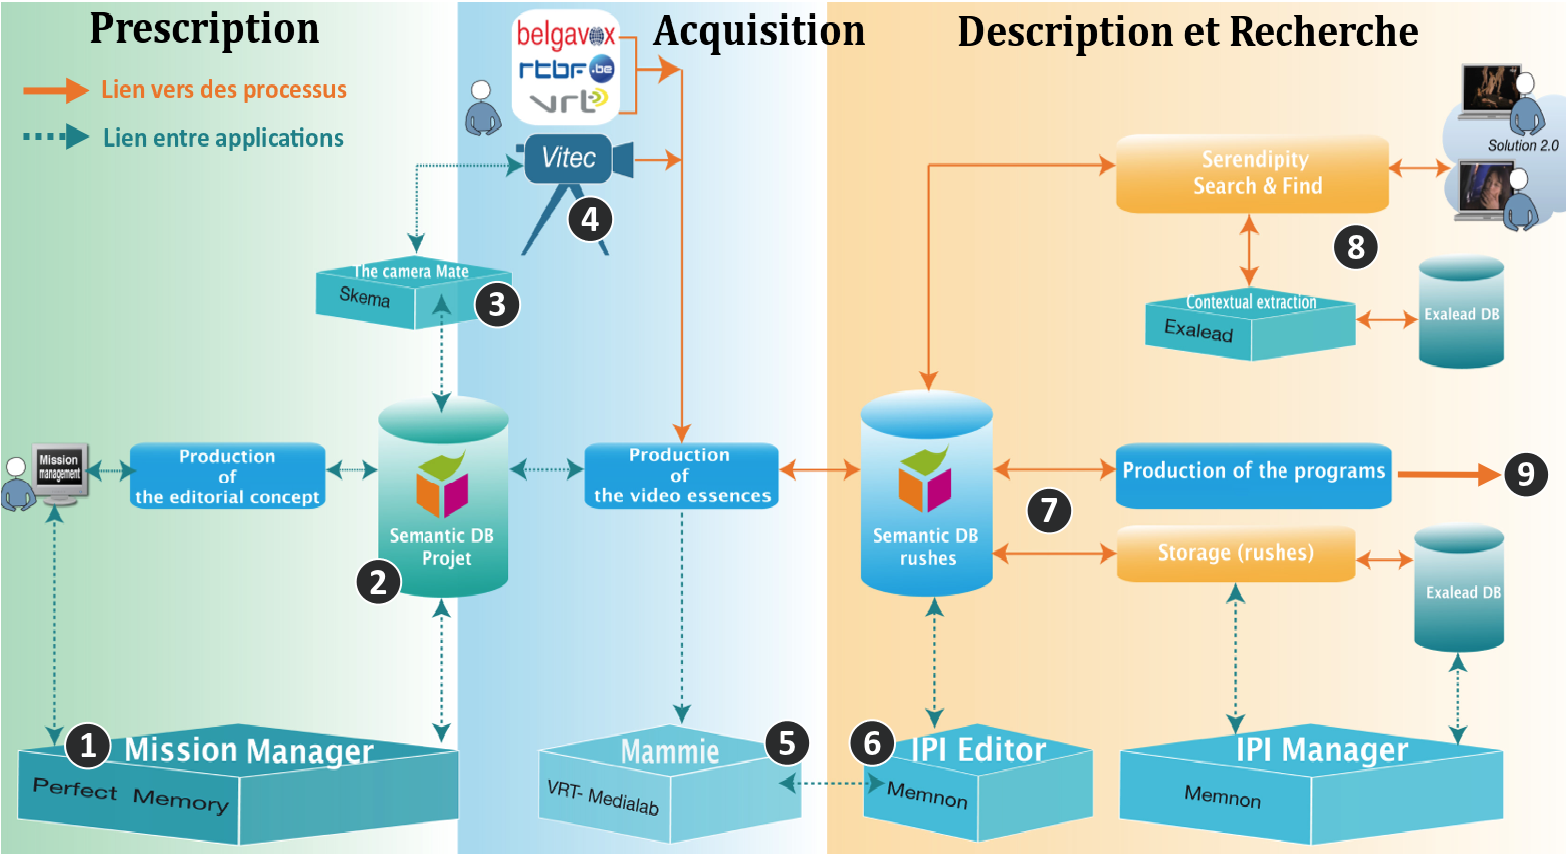
\includegraphics[width=1\textwidth]{./images/Architecture-process-v1.png}
\caption{Architecture finale du projet MediaMap : vue centrée sur le processus}
\label{img:arch-process}
\end{figure}

\begin{listenum}
	\item[(6)] L'acquisition du matériel et des connaissances aboutit à l'intégration de ces éléments à une plate-forme de gestion et de description côté RTBF. 
	La description est enrichi par des méthodes d'analyse automatique du signal ou des ajouts manuels, à différents moments de la post-production.
	Cela permet à l'équipe de post-production de la RTBF de prendre connaissance plus facilement du matériel filmé par ses contributeurs externes. [\g{Enrichissement des descriptions}]
	\co{L'\pc{IPI Editor} développé par Memnon se charge de cette intégration dans une base de stockage du matériel et une base sémantique pour gérer les connaissances qui y sont associées (à l'exception des connaissances sur le processus de production, gérées par le \pc{Mission Manager}.)e
	Parmi les traitements automatiques disponibles sur cette plate-forme, on trouve des analyseurs sonores qui permettent de repérer les moments de musique et de dialogue, et dans ce dernier cas de produire une transcription des paroles synchronisée mot à mot avec le flux audiovisuel.
	Il est également possible de rattacher des connaissances sur le monde au matériel, comme les personnes, les lieux etc.}

	\item[(7)] L'acquisition et la description du matériel audiovisuel peut être ensuite associée avec la structure documentaire du journal télévisé du soir, qui propose également une version Web, mais aussi à l'équipe de production d'un DVD de l'évènement (revoir la section \ref{sec:ex-reuse}, p.\pageref{sec:ex-reuse} pour plus de détails).
	Enfin, certaines séquences seront également mises à disposition à des organisations externes via la base sémantique de description des rush (prises de vue). [\g{Réutilisation}]
	\co{La réutilisation des matériaux audiovisuels dans divers contexte d'exploitation est rendu possible par l'articulation entre la plate-forme de stockage des rush et des bases sémantiques sur le processus de production (\pc{Mission Manager}) et sur les descriptions associées aux documents audiovisuels (\pc{IPI Editor, IPI Manager}), ce qui explique le positionnement de l'étape n°7 sur le diagramme.}

	\item[(8)] Lors du montage du sujet pour le journal télévisé, la RTBF se rend compte qu'ils ont besoin d'un plan de coupe présentant le lieu de représentation de l'évènement culturel, qui n'a pas été commandé aux équipes de tournage. 
	Pour cela, le monteur vérifie d'abord si les équipes de la VRT ou de la RTBF ne l'aurait pas tourné (en plus de la commande), mais aucun plan n'est disponible. 
	De ce fait, une recherche dans la base de rush (prise de vue) est lancée et le monteur récupère un plan existant. [\g{Accès et Recherche}]
	\co{L'interface de gestion du projet du \pc{Mission Manager} permet de visualiser le matériel produit par chaque équipe de tournage, de naviguer dans la structure documentaire du projet.
	La recherche de matériel passe d'abord par une phase d'indexation prise en charge par Exalead et rendu accessible à un interface Web construite par Solution 2.0.
	L'indexation s'effectue par une connexion à l'\pc{IPI Manager} qui gère l'évolution des connaissances sur et associées au document audiovisuel.
	Ces recherches s'effectue avec le même vocabulaire que la définition d'un plan dans un script, et renvoit non seulement à des séquences audiovisuelles, mais également à leur contexte de production (projet, contributeur, structure documentaire etc.). 
	La position de l'étape n°8 sur le diagramme présuppose l'échange d'information entre la base Exalead et la base sémantique de l'IPI Manager.}
	
	\item[(9)] Une fois le sujet pour le journal télévisé produit, la RTBF envoit le projet entier à la VRT, qui le réutilisera en modifiant le commentaire. 
	Ce transfert ne consiste pas simplement à envoyer le montage final, mais l'ensemble des rush, des montages intermédiaires, des commentaires du public flamand, des enrichissement de descriptions etc.
	Il s'agit donc d'un échange de matériel et de connaissances sur ce matériel. [\g{Transport, Échange}]
	\co{Les différentes bases sémantiques peuvent exporter les connaissances stockés afin de les transmettre à d'autres bases, en même temps que l'ontologie qui définit ces connaissances.
	Notre modèle doit également embarquer les variations de vocabulaire utilisé par le recepteur, afin de réaliser l'adaptation de leur expression.}
\end{listenum}



% En faire un tableau
La Table \ref{tab:archaine} clarifie la manière dont le scénario se déroule par rapport à une chaîne de production classique (voir \ref{sec:prod}). 
En effet, notre scénario met en avant de nouvelles pratiques, comme la production collaborative et la réutilisation de fragments dès leur production. 
Nous proposons donc de comparer notre scénario avec les étapes classiques d'un projet de production. 
Alors que la \g{préproduction} est représentée par les phases (1) et (2), les phases (3) et (4) n'existent pas en tant que telles dans un projet de production classique.
En effet, la traduction du script en guide de tournage doit être prise en charge par le contributeur, de même que les caméras ne propose habituellement pas d'assistance pendant le tournage ou de vérification après coup. 
Toutefois, on peut les assimiler à une étape de \g{fabrication} du matériel audiovisuel.
La phase (5) de livraison et (6) d'enrichissement des descriptions correspond à l'étape du \g{dérushing}. 
La phase (7) de réutilisation correspond à plusieurs étapes, puisqu'il s'agit à la fois du \g{montage} et de la \g{finition}. Dans le cas décrit, il s'agit de réutilisation dans le sens où les fragments participent à plusieurs projets de production. 
La phase (8) d'accès et recherche peut être présentée comme une étape \g{archivages} qui serait intégrée à la production. 
La phase (9) de transport et d'échanges peut être mise en rapport avec l'étape de \g{distribution}, quoi que la nature de l'objet échangé varie énormément (des fichiers vidéo ou bien une ensemble de connaissances et de fichiers représentant le projet de production).

\begin{table}
\begin{center}
\begin{tabular*}{0.92\textwidth}{|c|c|c|c|c|c|c|c|c|c|}
\hline
	\multicolumn{2}{|c|}{\g{Pré-production}} & \multicolumn{4}{|c|}{\g{Production}} & \multicolumn{2}{|c|}{\g{Post-production}} & \multicolumn{2}{|c|}{\g{Exploitation}} \\ \hline\hline
	\e{Planning} & \e{Scripting} & \multicolumn{2}{|c|}{\e{Fabrication}} & \multicolumn{2}{|c|}{\e{Derushing}} & \e{Montage} & \e{Finition} & \e{Archivage} & \e{Distribution} \\ \hline
	(1) & (2) & (3) & (4) & (5) & (6) & \multicolumn{2}{|c|}{(7,8)} & (8) & (9) \\ \hline

\end{tabular*}
\caption{Comparaison entre les étapes de le chaîne de production classique (\e{en italique}) et le scénario de production de MediaMap}\label{tab:archaine}
\end{center}
\end{table}


%%%%%%%%%%%%%%%%%%%%%%%%%%%%%%%%%%%%%%%%%%%%%%
%%%%%%%%%%%%%%%%%%%%%%%%%%%%%%%%%%%%%%%%%%%%%%
% \subsection{Architecture du projet MediaMap}\label{sec:arch-compo}
% % Nous présentons les particularités applicatives de l'approche MediaMap

% \begin{figure}[ht!]
% \centering
% 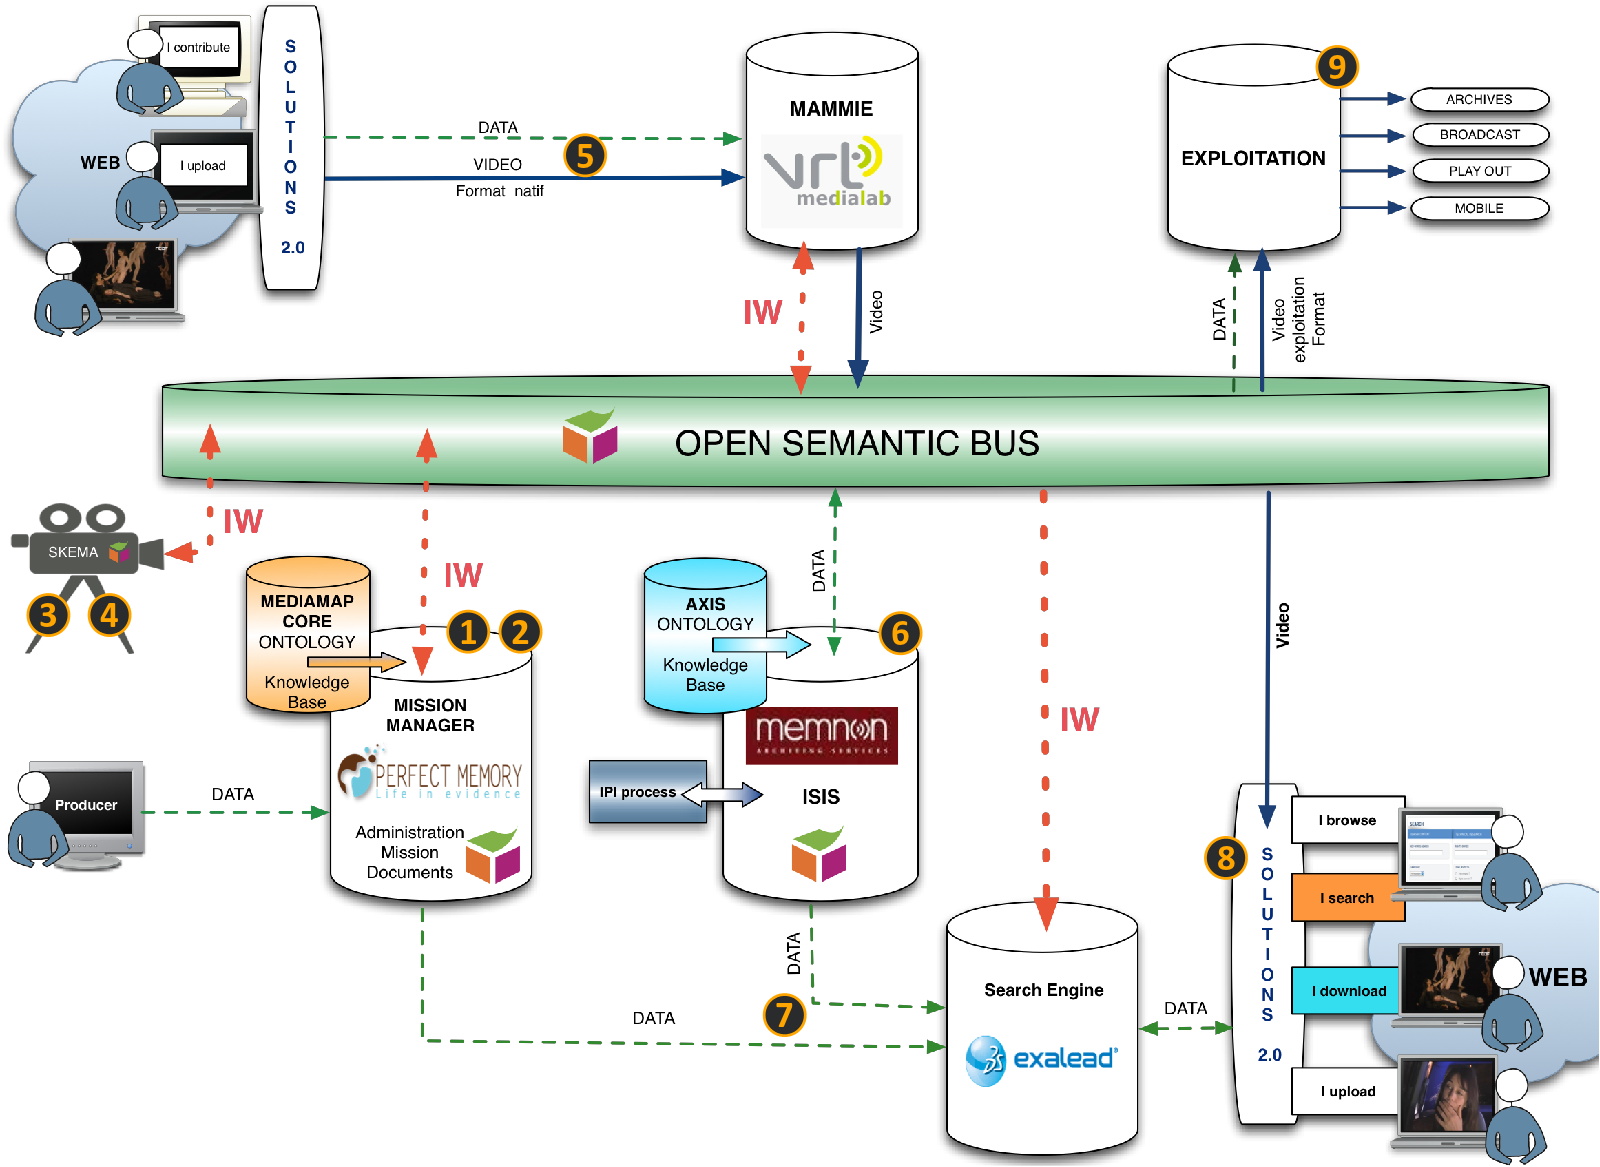
\includegraphics[width=1\textwidth]{./images/Architecture-apps-v1.png}
% \caption{Architecture finale du projet MediaMap : vue applicative des flux de données}
% \label{img:arch-apps}
% \end{figure}


% La Figure \ref{img:arch-apps} reprend la numérotation du scénario et propose une vue alternative centrée sur les flux de données entre les applications. 
% En particulier, l'apparition de l'\pc{Open Semantic Bus} (OSB) et des \pc{Interoperability Wicket} (IW, guichet d'interopérabilité) introduisent des éléments d'une architecture modulaire s'inspirant des architectures distribuées de réseau informatique.
% Un élément caché dans le diagramme est la notion de \pc{Unique Semantic Entity} (USE) qui correspond à un paquet automome de connaissances et qui constitue le format d'échange sur l'OSB.
% En pratique, OSB, IW et USE permettent de réaliser l'interopérabilité des échanges de données et de connaissances entre les applications de la chaîne de production audiovisuelle, regroupant ainsi les fonctions suivantes : 
% \begin{liste}
% 	\item gestion dynamique des applications connectées à l'OSB et des services proposées, à la manière des répertoires de Web Services, de façon à accepter l'ajout ou la suppression de ces derniers.
% 	Cela implique également de décrire les appels et les résultats fournis par ces services.
% 	Il s'agit par exemple de demander une description des formats d'import supportés par une application, d'une description des capacités d'un contributeur, ou bien de ces droits associés à un projet ou une tâche d'un projet.

% 	\item gestion des échanges de données entre applications et entre contributeurs par l'intermédiaire des IW. 
% 	Ces guichets assurent l'acquisition des données et leur comparaison éventuelle avec un attendu.
% 	Ensuite, suivant le destinataire, ils peuvent effectuer des transformations automatiques pour satisfaire aux besoins du récepteur. 
% 	Ces transformations opèrent sur deux niveaux, sur le plan du formatage des données (passage de XML à JSON, ou bien d'un modèle de données à l'autre), et sur le plan de l'expression des connaissances (transformation d'un vocabulaire professionnel en explication pour amateur par exemple).
% \end{liste}

% Parmi les différences avec la Figure précédente, il faut noter la mise en avant des interfaces Web créés par Solution 2.0. 
% Dans le cas de l'étape n°5, la livraison d'un matériel peut alors se faire indépendamment de la caméra "intelligente" et de l'OSB.
% Concernant, l'étape n°8 d'accès et de recherche de matériel, elle peut également être ouverte à des organisations externes.
% Un autre point important sont les différences de nommage. L'\pc{IPI Manager} et l'\pc{IPI Editor} était d'abord nommé ISIS par Memnon, mais ce nom fut changé en fin de projet pour des raisons commerciales. 
% De même, l'\pc{Axis ontology} est en réalité une version modifiée de l'ontologie MediaMap, intégrant des raffinements et des extensions spécifiques à leurs processus d'indexation. 
% Ainsi, l'ontologie construite pendant le projet est utilisée, modifiée et intégrée dans des applications, notamment celles de Memnon et de Perfect Memory.




\subsection{Axes de modélisation}\label{sec:axes}
Comme nous l'avons vu en section \ref{sec:metier}, la production audiovisuelle se présente comme un processus structuré en grandes étapes (pré-production, production, post-production) qui visent la préparation, la fabrication puis l'exploitation d'un document audiovisuel.
S'il existe une diversité de type de production (scriptée, non-scriptée) et de genre de documents (\ref{sec:strat-desc}), celles-ci ne représentent que des variations dans la réalisation des étapes de cette structure générale.  
De la même manière, les pratiques de production collaborative et de réutilisation du matériel existant (\ref{sec:rechaine}) n'entraînent pas de transformation profonde de cette structure, mais plutôt une adaptation de certaines étapes. 
Cependant, l'ouverture de la chaîne à de nouveaux contributeurs ainsi que le focus sur les fragments nécessitent d'affiner la modélisation classique du document audiovisuel et d'en suivre sa construction. 
Ainsi, s'il n'existe pas \e{une} production audiovisuelle, il nous faut modéliser des situations typiques de \e{la} production audiovisuelle, qui pourront s'ajuster aux spécificités \e{des} productions audiovisuelles.

% Notre travail de modélisation se heurte à deux verrous scientifiques, identifiés en section \ref{sec:scien} puis développés dans les chapitre \ref{chap:omod} et \ref{chap:mav}, que nous reformulons en : 
Nous décomposons les problèmes scientifiques que nous avons défini précédemment en deux axes de modélisation principaux. 
L'axe $\alpha$ se rapporte aux situations typiques de la production audiovisuelle (\ref{sec:situations}), alors que l'axe $\beta$ renvoit à des questions de représentation progressive de ces situations, ainsi qu'à la documentation de cette représentation.
Ce dernier axe ne conduit pas à la définition de patrons de conception, mais plutôt à l'enrichissement des patrons existants ainsi qu'à la mise en place de conventions de représentation qui sont distinctes de notre modèle.
Ainsi, leur mise en oeuvre se situe plus au niveau des applications que de l'ontologie que nous avons construites, ce qui nous amène à présenter certaines de ces éléments dans la section \ref{meo}.



\begin{problemes}{LightGoldenrodYellow}
\begin{liste}
 	\item[(\g{$\alpha$})] \g{L'articulation de plusieurs ensembles de connaissances} [\e{$\chi_1$ : autonomie}, \e{$\chi_2$ : réutilisabilité}]. 
 	On distingue ainsi deux ensembles de connaissances : 
 	% à quoi servent-ils ?
 	\begin{listeni} 
 		\item[($\alpha_1$)] L'organisation du \e{processus de production audiovisuelle}, qui décrit la répartition des tâches et  les capacités des \e{contributeurs}.
 		Cet ensemble permet d'associer les connaissances fabriquées par les contributeurs aux documents et de faciliter leur implication et les échanges de connaissances.
 		
 		\item[($\alpha_2$)] L'organisation du \e{document audiovisuel}, c'est-à-dire sa structure documentaire, le \e{matériel audiovisuel} qu'on y attache et une description de leur fabrication (l'\e{écriture filmique} détaillée dans le script).
 		Cet ensemble permet de faciliter la recherche, la gestion et donc la réutilisation des fragments audiovisuels.
 	\end{listeni}

 	\item[(\g{$\beta$})] \g{Une pro(duction/con)sommation progressive et contributive de ces connaissances} [\e{$\delta_1$: multi-jargon}, \e{$\delta_2$ : documentation}, \e{$\delta_3$ : évolution, gestion}].
 	Il s'agit ici du problème de l'évolution et du partage des connaissances liées à un document/fragment audiovisuel tout au long de son ou de ses cycle(s) de vie. 
 	On distingue deux écueils nouveaux suite à l'ouverture de la chaîne à des pratiques de réutilisation : la \e{progressivité de la description}, et la nécesssité de la rendre compréhensible malgré l'\e{hétérogénéité des contributeurs} : 
 	\begin{listeni}
 		\item[($\beta_1$)] \e{Les connaissances sur les document/fragments audiovisuels évoluent et doivent s'ajuster au contexte de production ou de réutilisation}.
 		Les connaissances fabriquées en début de chaîne de production prescrivent un résultat attendu, or de nombeux éléments sont susceptibles d'être modifiés ou précisés par la suite.
 		Il faut donc ajuster les connaissances prescriptives à la réalité des opérations, afin de décrire les résultats effectifs (et non plus l'attendu).
 		Cet écueil apparent est en réalité une opportunité, car la fabrication des descriptions peut alors s'appuyer sur les connaissances prescriptives et les vérifier. 
		De plus, la réutilisation d'un fragment/document audiovisuel dans un nouveau contexte n'implique pas seulement un transfert de matériels audiovisuels, mais également un transfert des connaissances. % mais est-ce que l'on traite vraiment ce cas ? on gère des ensembles de connaissances qui peuvent évoluer (enrichissement)
		Ce transfert peut nécessiter d'extraire certaines connaissances toujours pertinentes et de les associer à celles du nouveau contexte d'utilisation, ou bien de les intégrer à une conceptualisation propre à ce contexte (spécialisation ou bien extension).
		% Cette évolution est rendue possible par 

		\item[($\beta_2$)] \e{Adapter la forme d'expression des connaissances en fonction de l'implication du contributeur dans la chaîne de production et de ses capacités.}
 		Le problème de l'accès aux connaissances est traité par la composition d'une vue contextuelle et spécifique à chaque contributeur de la chaîne, ou chaque groupe de contributeurs.
 		Toute connaissance exprimée à travers le modèle doit pouvoir être caractérisée suivant les codes d'écritures utilisés, eux-mêmes reliées aux capacités des contributeurs.
		Il est alors possible d'effectuer une double sélection ; les connaissances pertinentes suivant l'implication dans la chaîne (en utilisant la description du processus de production); les formes d'expression facilitant leur compréhension (à partir d'une description des capacités des contributeurs).
		% Cette adaptation est rendue possible par le couplage entre conceptualisation, terminologie et documentation.
 	\end{listeni}
\end{liste}
\end{problemes}


Nous pouvons raffiner maintenant ces deux axes de modélisation. 
Voici les situations typiques de la production audiovisuelle que nous avons modélisé en patrons de conception : 
% \begin{problemes}s{LightGoldenrodYellow}
\begin{listeni}
	\item[($\alpha_1$)] l'organisation du \g{processus de production} (\ref{sec:mission}) et du travail de ses \g{contributeurs} (\ref{sec:agent}): 
	\begin{liste}
		\item[($\alpha_1a$)] la division d'un projet de production en sous-tâches et la spécification du résultat attendu ainsi que des moyens fournis pour les remplir .

		\item[($\alpha_1b$)] l'assignation des tâches d'un projet à des contributeurs, ce qui leur confère un rôle, des droits et des responsabilités.
	\end{liste}

	\item[($\alpha_2$)] l'articulation d'un \g{document audiovisuel} et de ses différentes composantes (\ref{sec:opus}), avec leurs descriptions (\ref{sec:annotation}) : 
	\begin{liste}
		\item[($\alpha_2a$)] la gestion des fichiers qui encapsulent le matériel audio-visuel et ces différentes pistes.
		\item[($\alpha_2b$)] la segmentation du matériel audiovisuel.
		\item[($\alpha_2c$)] la structure documentaire qui suit des règles de composition de fragments. 
		\item[($\alpha_2d$)] la description par l'écriture filmique, et ses références à des éléments fictifs ou réels.
	\end{liste}
\end{listeni}
% \end{problemes}


Concernant les aspects concernant la documentation et l'évolution des connaissances : 
\begin{listeni}
\item[($\beta_1$)] Le déroulement de la production a pour conséquence de faire \g{évoluer nos connaissances} sur l'organisation du processus de production et l'articulation du document audiovisuel : 
	\begin{liste}
		\item L'évolution de la description d'un document audiovisuel.
		\item L'échange de connaissances entre organisations.
		\item Les pratiques de réutilisation de fragments documentaires.
	\end{liste}

	\item[($\beta_2$)] L'\g{adaptation des formes d'expressions} aux capacités des contributeurs de la chaîne de production : 
	\begin{liste}
		\item La mise en place d'un thésaurus multi-jargon et d'une documentation des concepts.
		\item L'attribution de compétences linguistiques et professionnelles aux contributeurs (humains, machines).
		\item L'accès personnalisé aux connaissances de la chaîne suivant le contexte (le contributeur, ses capacités, son implication dans la châine).
	\end{liste}
\end{listeni}

\begin{figure}[ht!]
\centering
\includegraphics[width=0.8\textwidth]{./images/Legende-v1.png}
\caption{Légende pour les diagrammes de présentation des patrons de conception}
\label{img:legende}
\end{figure}

Nous avons rappelé les indicatifs de ces axes de modélisation dans les titre des sections suivantes.
Par ailleurs, nous avons utilisé deux types de Figure pour présenter ces patrons (voir Figure \ref{img:legende}) : 
\begin{liste}
	\item les Figures de type \gui{Principaux concepts et relations} permettent de présenter les relations entre concepts pour représenter une situation. 
	Dans certains cas, nous avons ajouté des liens de spécialisation afin de donner directement une vue synoptique sur les possibilités de représentation de ce patron. 
	Les propriétés des concepts sont généralement définis dans le texte.

	\item les Figures de type \gui{Extrait de la structure ontologique} se focalisent sur les liens de spécialisations entre concepts, et permettent de préciser les différences entre concepts frères ainsi que la similarité entre concepts parent-enfants utilisées dans la méthode de construction d'ontologie \pc{Archonte} (\ref{sec:construction}).
	Ces Figures permettent de détailler la formalisation de notre modèle conceptuel. 
	Des exemples d'instanciations seront ensuite présentés dans la section \ref{sec:meo}.
\end{liste}
\input{CONTENU/2-contrib/2a-concepts}
\input{CONTENU/2-contrib/2b-concepts}



% % \cleardoublepage


% %%%%%%%%%%%%%%%%%%%%%%%%%%%%%%%%%%%%%%%%%%%%%%%%%%%%%%%%%%%%%%%%%%%%%%%%%%%%%%%%%%%%%%%%%%%%%%%%%%%
% %%%%%%%%%%%%%%%%%%%%%%%%%%%%%%%%%%%%%%%%%%%%%%%%%%%%%%%%%%%%%%%%%%%%%%%%%%%%%%%%%%%%%%%%%%%%%%%%%%%
\part*{Discussion}
\addcontentsline{toc}{part}{Discussion}
\chapter{Applications, expérimentations et validation}\label{chap:app}
\minitoc
% % Le modèle évolue en fonction des besoins des membres du projet MediaMap. Les développeurs des applications sont susceptible d"étendre ou d'affiner le modèle suivant les besoins qu'ils rencontrent. Il ne s'agit pas encore d'un standard figé mais bien d'un effort en cours et en collaboration avec les utilisateurs. Nous nous efforçons donc d'adopter une modélisation et un vocabulaire proche de leur contexte de travail en vue de privilégier l'adoption du modèle, son utilisation et sa réappropriation. Ensuite, il s'agit de formaliser la modélisation afin de pouvoir l'opérationnaliser et développer des applications qui produisent des descriptions suivant ce modèle ou se nourrissent d'elles pour restituer une perspective métier à ces utilisateurs. 
\section{Applications du projet MediaMap}\label{sec:app}
\section{Expérimentations du projet MediaMap}\label{sec:xp}

\section{Mise en oeuvre}\label{sec:meo}
\subsection{Choix d'un langage}\label{sec:ln}
\subsection{Opérationnalisation}\label{sec:op}

\section{Validation}\label{sec:val}
\subsection{Patrons d'utilisation}
\cite{Isaac2005}

% demande/délégation/assignation d'une tâche, de droits, à un contributeur
% hiérarchie d'activité dans un projet
% fragmentation documentaire 
% segmentation du matériel av
% articulation entre activité et résultat
% description (a priori et a posteriori) d'un fragment documentaire et du matériel audiovisuel
% documentation d'une conceptualisation
% attribution de compétences à un contributeur
% sélection de la documentation suivant les compétences (et/ou) l'implication d'un contributeur dans un projet
% articulation base de faits, documentation, conceptualisation


\chapter*{Conclusion}\label{chap:cc}
\addcontentsline{toc}{chapter}{Conclusion}

% \chapter{}\label{c:}
% \section{}\label{s:}

% \cleardoublepage

%%%%%%%%%%%%%%%%%%%%%%%%%%%%%%%%%%%%%%%%%%%%%%%%%%%%%%%%%%%%%%%%%%%%%%%%%%%%%%%%%%%%%%%%%%%%%%%%%%%
%%%%%%%%%%%%%%%%%%%%%%%%%%%%%%%%%%%%%%%%%%%%%%%%%%%%%%%%%%%%%%%%%%%%%%%%%%%%%%%%%%%%%%%%%%%%%%%%%%%
%%%%%%%%%%%%%%%%%%%%%%%%%%%%%%%%%%%%%%%%%%%%%%%%%%%%%%%%%%%%%%%%%%%%%%%%%%%%%%%%%%%%%%%%%%%%%%%%%%%
%%%%%%%%%%%%%%%%%%%%%%%%%%%%%%%%%%%%%%%%%%%%%%%%%%%%%%%%%%%%%%%%%%%%%%%%%%%%%%%%%%%%%%%%%%%%%%%%%%%
%%%%%%%%%%%%%%%%%%%%%%%%%%%%%%%%%%%%%%%%%%%%%%%%%%%%%%%%%%%%%%%%%%%%%%%%%%%%%%%%%%%%%%%%%%%%%%%%%%%
%%%%%%%%%%%%%%%%%%%%%%%%%%%%%%%%%%%%%%%%%%%%%%%%%%%%%%%%%%%%%%%%%%%%%%%%%%%%%%%%%%%%%%%%%%%%%%%%%%%
%%%%%%%%%%%%%%%%%%%%%%%%%%%%%%%%%%%%%%%%%%%%%%%%%%%%%%%%%%%%%%%%%%%%%%%%%%%%%%%%%%%%%%%%%%%%%%%%%%%
%%%%%%%%%%%%%%%%%%%%%%%%%%%%%%%%%%%%%%%%%%%%%%%%%%%%%%%%%%%%%%%%%%%%%%%%%%%%%%%%%%%%%%%%%%%%%%%%%%%
%%%%%%%%%%%%%%%%%%%%%%%%%%%%%%%%%%%%%%%%%%%%%%%%%%%%%%%%%%%%%%%%%%%%%%%%%%%%%%%%%%%%%%%%%%%%%%%%%%%
%%%%%%%%%%%%%%%%%%%%%%%%%%%%%%%%%%%%%%%%%%%%%%%%%%%%%%%%%%%%%%%%%%%%%%%%%%%%%%%%%%%%%%%%%%%%%%%%%%%
%%%%%%%%%%%%%%%%%%%%%%%%%%%%%%%%%%%%%%%%%%%%%%%%%%%%%%%%%%%%%%%%%%%%%%%%%%%%%%%%%%%%%%%%%%%%%%%%%%%
% \appendix
% \part*{Annexes}
% \rehead{\headingsf\scshape Annexe~\thechapter}
% \noappendicestocpagenum
% \addappheadtotoc

% \cleardoublepage

%%%%%%%%%%%%%%%%%%%%%%%%%%%%%%%%%%%%%%%%%%%%%%%%%%%%%%%%%%%%%%%%%%%%%%%%%%%%%%%%%%%%%%%%%%%%%%%%%%%
%%%%%%%%%%%%%%%%%%%%%%%%%%%%%%%%%%%%%%%%%%%%%%%%%%%%%%%%%%%%%%%%%%%%%%%%%%%%%%%%%%%%%%%%%%%%%%%%%%%
%%%%%%%%%%%%%%%%%%%%%%%%%%%%%%%%%%%%%%%%%%%%%%%%%%%%%%%%%%%%%%%%%%%%%%%%%%%%%%%%%%%%%%%%%%%%%%%%%%%
% \chapter{D'un Web à l'autre : les paradigmes de la lecture informatique}\label{a:webs}
% \KOMAoptions{twoside=no}

\pagestyle{empty}

\input{PERRON/GARDE}

% \newpage

% ~

% \cleardoublepage

% \pagestyle{empty}

% \input{PERRON/REMERCIEMENTS}

% \cleardoublepage

% \KOMAoptions{twoside=yes}

\frontmatter

\pagestyle{scrheadings}

\shorttableofcontents{Sommaire}{2}

\cleardoublepage


%%%%%%%%%%%%%%%%%%%%%%%%%%%%%%%%%%%%%%%%%%%%%%%%%%%%%%%%%%%%%%%%%%%%%%%%%%%%%%%%%%%%%%%%%%%%%%%%%%%
%%%%%%%%%%%%%%%%%%%%%%%%%%%%%%%%%%%%%%%%%%%%%%%%%%%%%%%%%%%%%%%%%%%%%%%%%%%%%%%%%%%%%%%%%%%%%%%%%%%


% \pagestyle{empty}

% ~

% \bigskip

% \vspace{11em}

% \bigskip

% \epigraphii{La totalité est la non vérité.}{Adorno, \ita{Minima Moralia}}

% \cleardoublepage
% \addcontentsline{toc}{part}{État de l'Art}
% \pagestyle{empty}

% ~
% \bigskip

% \vspace{11em}

% \bigskip

% \epigraphii{Se demander si un ordinateur peut penser ... est aussi intéressant que de se demander si un sous-marin peut nager.}{ Edsger Wybe Dijkstra, \ita{The threats to computing science}}

% \pagestyle{scrheadings}

%%%%%%%%%%%%%%%%%%%%%%%%%%%%%%%%%%%%%%%%%%%%%%%%%%%%%%%%%%%%%%%%%%%%%%%%%%%%%%%%%%%%%%%%%%%%%%%%%%%
%%%%%%%%%%%%%%%%%%%%%%%%%%%%%%%%%%%%%%%%%%%%%%%%%%%%%%%%%%%%%%%%%%%%%%%%%%%%%%%%%%%%%%%%%%%%%%%%%%%
\part*{Exposition}
\addcontentsline{toc}{part}{Exposition}

\mainmatter
%%%%%%%%%%%%%%%%%%%%%%%%%%%%%%%%%%%%%%%%%%%%%%%%%%%%%%%%%%%%%%%%%%%%%%%%%%%%%%%%%%%%%%%%%%%%%%%%%%%
%%%%%%%%%%%%%%%%%%%%%%%%%%%%%%%%%%%%%%%%%%%%%%%%%%%%%%%%%%%%%%%%%%%%%%%%%%%%%%%%%%%%%%%%%%%%%%%%%%%
% \section*{Préambule (n)}
% \addcontentsline{toc}{section}{Préambule}



%%%%%%%%%%%%%%%%%%%%%%%%%%%%%%%%%%%%%%%%%%%%%%%%%%%%%%%%%%%%%%%%%%%%%%%%%%%%%%%%%%%%%%%%%%%%%%%%%%%
%%%%%%%%%%%%%%%%%%%%%%%%%%%%%%%%%%%%%%%%%%%%%%%%%%%%%%%%%%%%%%%%%%%%%%%%%%%%%%%%%%%%%%%%%%%%%%%%%%%
\chapter{Introduction}\label{chap:intro}
\minitoc
% \epigraphii{On peut s'étonner que les actes spontanés par lesquels l'homme a mis en forme sa vie, se sédimentent au dehors et y mènent l'existence anonyme des choses. La civilisation à laquelle je participe existe pour moi avec évidence dans les ustensiles qu'elle se donne.}{Merleau-Ponty\\\hfill\ita{Phénoménologie de la perception}}

%%%%%%%%%%%%%%%%%%%%%%%%%%%%%%%%%%%%%%%%%%%%%%%%%%%%%%%%%%%%%%%%%%%%%%%%%%%%%%%%%%%%%%%%%%%%%%%%%%%
% \section{Contexte}\label{chap:contexte}
Le travail de thèse dont nous rendons compte dans ce mémoire s'est déroulé dans le cadre du projet MediaMap\footnote{Voir \url{http://www.mediamapproject.org/}} soutenu par le cluster européen Eureka Celtic et la Direction Générale de la Compétitivité, de l'Industrie et
des Services (DGCIS) du ministère de l'Economie, des finances et de l'industrie.
La participation à ce projet de recherche et développement nous a imprégnés de connaissances sur la production audiovisuelle.
%, les besoins qui émergent des tendances actuelles et les problèmes rencontrés pour les combler. 



%Nous nous intéresserons ensuite (\g{Chapitre \ref{chap:problo}}) aux 


%%%%%%%%%%%%%%%%%%%%%%%%%%%%%%%%%%%%%%%%%%%%%%%%%%%%%%%%%%%%%%%%%%%%%%%%%%%%%%%%%%%%%%%%%%%%%%%%%%%
\section{L'impact du numérique sur l'audiovisuel}\label{sec:motiv}
\e{
La révolution numérique initiée depuis une trentaine d'années en conjonction avec la révolution électronique et informatique, s'est progressivement imposée à tous types d'information et de contenus. 
%jusqu'à devenir prépondérante et indispensable dans un monde informatisé.
Ces mouvements d'informatisation des pratiques et de numérisation de l'information impactent les organisations et les métiers en redistribuant les tâches entre humains et machines. 
Dans le cadre de cette thèse, nous nous pencherons sur le cas de l'audiovisuel et de la numérisation de ce contenu et des informations associées.}

%L'audiovisuel représente à plus d'un titre un objet singulier.
%l'exploitation des contenus numériques est en passe de s'étendre à toutes les étapes du cycle de vie d'un objet audiovisuel. % ? pourquoi exploitation ?
Après une informatisation des étapes de postproduction (logiciels de montage, effets spéciaux etc.) puis des équipements de captation (caméra, micro etc.) et de la distribution du côté des diffuseurs, nous avons connu une véritable explosion d'appareils destinés au grand public (lecteur multimédia portable, appareil photo, téléphone portable, dictaphone etc.).


Plusieurs grands chantiers s'ouvrent désormais dans ce mouvement d'informatisation des étapes de la chaîne de production :
\begin{liste}
	\item L'archivage des contenus de manière à les faire entrer dans l'histoire malgré la dégradation inexorable des supports. 
	Il ne s'agit pas simplement de leur permettre de survivre jusqu'à la prochaine génération d'appareils électroniques, mais également de garantir leur \ciel{lisibilité technique et culturelle}, (\cite[p.~12]{Bachimont2000}).

	\item La préproduction des contenus qui est presque inexistante et qui permettrait de récolter des informations sur les contenus avant même leur fabrication. 
	L'enjeu plus général est d'initier l'indexation des contenus au moment du \e{Scripting} et de la continuer tout au long de la chaîne, chaque étape pouvant rajouter des informations ou bien réévaluer les anciennes.
\end{liste}

À côté de la numérisation et de l'informatisation, il ne faudrait pas oublier le développement considérable des réseaux de télécommunications qui a grandement favorisé les échanges de contenus de manière illégale ou légale, de pairs à pairs (\e{Peer to Peer}), entre diffuseurs et spectateurs (\e{Business to Consumers}) ou entre acteurs professionnels de la chaîne (\e{Business to Business}). 
Ainsi, numérisation et informatisation sont dorénavant implictement associées aux facilités de transfert de ces réseaux. 

Sans tenter de tirer toutes les conséquences de ces révolutions technologiques (électronique et informatisation, numérisation, mise en réseaux) sur les usages des spectateurs et des acteurs de la chaîne de production audiovisuelle, on retiendra trois constats important qui charpentent notre réflexion : 
\begin{liste}
	\item \eg{il existe un nombre croissant de contenus audiovisuels en circulation.}
	L'offre et la demande augmentent de même que les capacités de transfert des réseaux et la généralisation des appareils électroniques de captation et de visionnage.

	\item \eg{les pratiques en lien avec les contenus audiovisuels se développent et s'individualisent.}
	La consommation de ces contenus se joue de plus en plus à un niveau individuel depuis l'apparition d'appareils personnels de communication et de visionnage. 
	De même, la production de contenus est facilité par l'informatisation et les progrès des appareils électroniques de captation. 
	La création de contenus n'est donc plus l'apanage de grandes équipes spécialisées et lourdement équipées.
	
	\item \eg{la numérisation complique le maintien de l'unicité des contenus audiovisuels}. 
	%Le principe même du numérique (\ciel{ça a été manipulé} [Bachimont2010]) repose sur la représentation de l'information et le calcul. 
	L'environnement numérique, par rapport à l'analogique, est plus propice à la copie, le transfert, la fragmentation et la manipulation des contenus ramenés invariablement à une donnée muette quelle que soit sa nature (texte, son, image animée ou non etc.) ou sa signification.
	Ainsi coupé des sens et du sens, les contenus semblent perdre leur identité dans le \gui{monomédia} numérique (\cite[p.~13]{Bachimont2000}) dans lequel on a peine à les gérer pour ce qu'ils représentent. 	

	%plus manipulables au sens où chaque visionnage construit une forme perceptive du contenu 

	%est une reconstruction de leur forme perceptible par des appareils de . Il y a donc par définition une certaine instabilité 
	%mobile, versatile, altérable, mouvant, variable, instable
\end{liste} 

%Le développement de l'électronique a ainsi favorisé une  le nombre de contenus audiovisuels, à favoriser leur circulation
%On constate ainsi une augmentation des sources de contenus ainsi qu'une intensification de leur circulation qui ont des conséquences sur les usages des spectateurs et les acteurs de la chaîne de production.
Nous allons maintenant préciser cet argumentaire et présenter les enjeux posés par la numérisation, l'informatisation et le développement de l'électronique.




%%%%%%%%%%%%%%%%%%%%%%%%%%%%%%%%%%%%%%%%%%%%%%%
\subsection{La numérisation des contenus audiovisuels}\label{sec:num}
Le contenu audiovisuel est avant tout un objet temporel, c'est-à-dire un flux d'images et de sons qui s'écoule en un temps donné. 
Un des enjeux liés à l'audiovisuel constitue alors à trouver une technologie d'enregistrement et de manipulation de ces flux.

\paragraph{L'enregistrement analogique du flux}
Les techniques d'enregistrement analogique reposent sur la conversion continue du flux original en un signal analogue dont les variations s'effectuent sur une échelle physique différente, par exemple une fréquence sonore transformée en une tension électrique. 
L'enregistrement s'effectue sur différents types de supports, cassettes magnétiques, films argentiques etc. 
La caractéristique commune de ces supports est que l'accès au contenu enregistré ne peut se faire que de manière linéaire ou séquentielle, c'est-à-dire qu'il faut avancer ou rembobiner la bande jusqu'au point de départ avant de pouvoir commencer la lecture. 
Ainsi, chaque opération de manipulation de ces contenus compte toujours un temps pas forcément négligeable consacré à l'alignement avec le point de départ désiré. 
Pour bien s'en rendre compte, il suffit de se souvenir du temps qu'il fallait pour rembobiner la cassette de votre film préféré, puis du temps passé en avance rapide pour passer les inévitables publicités précédant le film.

\paragraph{Numérisation et délinéarisation de l'accés}
Avec le numérique, cette expérience autrefois familière a complètement disparu et se voit remplacée par un accès immédiat à n'importe quel moment du contenu audio-visuel. 
La numérisation des contenus consiste à discrétiser le flux en un ensemble de valeurs que l'on convertit ensuite en flux binaire. Ce flux est ensuite enregistré sur des supports de mémoire magnétiques (disquettes 3'1/2, disques durs etc.) optiques (CD, DVD etc.) ou électronique (mémoire vive dite RAM, mémoire flash etc.). 
Seules ces dernières garantissent un accès arbitraire ou délinéarisé aux données stockées en mémoire (n'importe quelle donnée, à n'importe quel moment). 
Les supports magnétiques et optiques proposent un accés séquentiel comme l'analogique, mais plus rapide et surtout que l'on peut coupler avec les mémoires électroniques afin de se rapprocher de leurs performances.

\paragraph{Fragmentation}
Par ailleurs, au-delà des avantages liées aux temps d'accès au contenu, le numérique facilite également sa fragmentation et sa manipulation.
Contrairement à l'analogique, le numérique permet de représenter de manière arbitraire tout type d'information puis d'effectuer des calculs sur ces représentations. 
Ainsi, on peut associer au contenu audiovisuel d'autres contenus de différentes natures pour les enrichir et faciliter son exploitation ultérieure.

\paragraph{Discrétisation}
La discrétisation du flux audiovisuel quant-à-elle remet en cause la temporalité du contenu et permet de ce fait une fragmentation plus aisée et plus fine. 
Lorsque l'analogique effectue une transformation continue et analogue, le numérique définit une fréquence d'échantillonnage et quantifie les valeurs de la source sur une échelle arbitraire finie. 
C'est donc véritablement la fréquence d'échantillonnage qui constitue la première unité de réprésentation de l'information au-dessus du bit.
C'est donc en décidant du nombre de pixels pour représenter une image, ou aux nombres de valeurs par secondes prises pour représenter un son que l'on décide d'une première échelle de fragmentation. 
% Premier niveau de manip technique, ensuite il y a des USI
Toute autre fragmentation à l'échelle supérieure est potentiellement (re)constructible par calcul, pour autant qu'on possède une méthode opérationnalisable. 
%De même que chaque élément de cette fragmentation, chaque unité, devient adressable et donc manipulable par calcul. 
%\cite{Bachimont2000} parle ainsi d'utm, usi ...
% COUPURE DU SENS ?

% \g{== Révision à faire, introduire les UTM et USI ==}
\paragraph{Numériser, c'est informatiser le métier}
Parmi toutes les fragmentations possibles, il convient alors de déterminer leur pertinence par rapport aux types de calculs que l'on souhaite réaliser à chaque étape de la chaîne de production. 
Il s'agit ici de contrôler les calculs à effectuer en suivant les règles du métier qui en disposera.
Chaque étape ayant ses objectifs propres, les calculs effectués varient et s'opèrent à différents niveaux de fragmentation. 
Or la numérisation des contenus et de l'information s'effectue toujours en vue de leur manipulation par des programmes informatiques.
Ainsi, la numérisation entraîne toujours une informatisation qui impacte le métier dans son organisation et ses pratiques parce qu'il transforme les possibilités techniques qui le concerne.
% L'enjeu est donc double, d'une part identifier les niveaux de fragmentation pertinents pour chaque étape de la chaîne de production, et d'autre part de se donner les moyens de reconstruire la cohérence . 

% numériser => (a) fragmenter + (b) mettre en réseau => (a) besoin de conserver la cohérence de l'ensemble + (b) besoin d'autonomiser pour une future situation d'usage





%%%%%%%%%%%%%%%%%%%%%%%%%%%%%%%%%%%%%%%%%%%%%%%
\subsection{Le développement de l'électronique et des réseaux de télécommunications}\label{sec:electro}

L’explosion des appareils multimédia et des possibilités de transférer des contenus par les réseaux de télécommunication a promu de nouvelles pratiques de consommation et d'échanges des contenus tant chez les professionnels de l'audiovisuel que dans le grand public.

Du côté des professionnels, on voit ainsi l’émergence de systèmes de production qui utilisent le réseau pour faire transiter les contenus entre les systèmes d'information de leurs différents départements. 
Ces systèmes reprennent les principes d'architecture multi-tiers utilisés sur le Web avec les contenus représentés par des fichiers ou des flux binaires, d'où leur appelation de \e{file-based production system}.

Ce genre de système favorise également l’échange de fichiers entre organisations, puisque l’architecture permet d'exposer les données stockées de la même manière sur un réseau interne (intranet) ou externe (extranet, Internet).

Du côté du grand public, les appareils portables acquièrent de plus en plus de connectivité avec leur environnement et les réseaux. 
De simples lecteurs à brancher en USB, les appareils sont passés au stade communicant avec la 3G, le Wifi ou le Bluetooth. 
La fonction d'échange se banalise et inversement, les appareils communicant comme les téléphones deviennent eux-même des stations multimédia à part entière, musique, photo, vidéo, courriel, sms etc.\\


Un autre facteur à noter, est que ces appareils portables sont personnels, c’est-à-dire qu’ils sont majoritairement utilisés par un seul individu contrairement à l’usage du téléviseur qui était et reste encore largement un objet collectif. 
Une autre distinction fondamentale se situe dans le fait que ce sont des appareils informatiques qui fonctionnent entièrement dans le numérique. 
Les possibilités d’interaction en font non plus de simples terminaux de lecture, mais potentiellement de véritables instruments de création et de communication. En effet, l'insertion de données et la capture de contenus (photos, sons, textos etc.) est prévu et le couplage avec des plates-formes de publication (réseaux sociaux, dépôts de contenus, CMS etc.) est de mieux en mieux réalisé.

De ce fait, en plus des capacités toujours plus importante de consommation de contenus, ces appareils favorisent eux aussi leur circulation ou la circulation d’information annexes. 
Le partage d’opinions s’est considérablement développé avec la vague d'applications Web dites sociales qui permettaient aux utilisateurs de créer du contenu sans avoir à maîtriser les arcanes techniques du Web. 
Cet ajout d’opinion, même s’il est parfois réduit au minimum à une marque d'appréciation, implique ainsi l’utilisateur dans le processus de diffusion du contenu en le portant à l'attention d'autres utilisateurs (ses contacts dans le cas des réseaux sociaux, ses lecteurs dans le cas d'un weblog ou autres CMS, un ensemble d'utilisateurs anonymes dans le cas de services sociaux tels que Delicious\footnote{Delicious : \url{http://delicious.com/} est une plate-forme de sauvegarde, d'indexation par mot-clé et de partage de marques-pages. Pour l'utilisateur il s'agit soit de sauvegarder et d'indexer ses marques-pages, soit de découvrir les marques-pages correspondant à tel ou tel mot(s)-clé(s) déjà sauvegardées par la communauté. Les grandes tendances d'indexation sont ainsi accessibles à tous, tout en permettant à chacun de développer son système d'indexation personnelle -- adaptation française du mot anglais \e{folksonomy}. Il est également possible de partager directement ses trouvailles avec d'autres utilisateurs par un système d'abonnement et de notification.} ou Digg \footnote{Digg : \url{http://digg.com/} est un site de marque-page social qui fonctione sur le principe du vote. Un utilisateur peut proposer une page qui est alors soumise aux votes des autres utilisateurs. Suivant le succès de la page, celle-ci sera mise en avant sur la page principale de Digg, ou bien mise de côté avec le reste des pages moins populaires, et finira par être supprimée.}).\\


Les appareils numériques multimédia possèdent également des capteurs de plus en plus performant et de moins en moins coûteux qui permettent au grand public de découvrir de nouvelles activités de création (photographie et retouche d’image, tournage et montage vidéo, prise de son et mixage audio etc.).
Cet abaissement du coût d’entrée dans la production a favorisé l'émergence d’une production amateur hétéroclite qui va du passant prenant une photo d’un évènement se déroulant devant ses yeux jusqu’à l’amateur qui pratique par amour mais avec l'exigence d’un professionnel. 
Cette production amateur rentre alors en concurrence avec la production professionnelle, voire la remplace dans certains cas (lorsqu’un passant est le seul témoin d’un évènement inattendu par exemple). 
La concurrence est d'autant plus forte depuis l’apparition de plates-formes de partages qui facilitent la distribution des contenus. 
De manière générale, l’opposition classique entre producteurs et consommateurs se brouille et les professionnels cherchent de plus en plus à mettre à contribution les amateurs dans leurs processus. 
On se dirige ainsi vers un modèle où professionnels et amateurs contribuent à divers degrés et divers moments au cycle de vie des contenus.\\


Avec l'informatisation des appareils multimédia s’est introduit la possibilité de personnaliser la communication avec l'utilisateur, d'y ajouter de l'interactivité et de connecter les utilisateurs entre eux. 
Ces nouvelles possibilités transforment les attendus et les pratiques du grand public. 
De ce fait, cela impacte les rapports avec les professionnels qui tendent à vouloir intégrer les contributions externes à leurs propres productions. 
Ainsi, il ne s’agit plus simplement de produire des contenus qui s'adressent indistinctement aux masses, mais de trouver des moyens de personnaliser son offre, de recommander des contenus, de faciliter la récupération de contenus, de diversifier les occasions de consommer ou de contribuer.








%%%%%%%%%%%%%%%%%%%%%%%%%%%%%%%%%%%%%%%%%%%%%%%
\section{Le projet MediaMap}\label{sec:mm}
% %%%%%%%%%%%%%%%%%%%%%%%%%
\paragraph{Objectifs}
Le projet MediaMap vise à développer des modèles et des applications pour promouvoir la production audiovisuelle collaborative articulant contenus professionnels et amateurs. 
En particulier, l'ambition est d'intégrer les amateurs et leurs contenus dans la chaîne de production professionnelle en améliorant d'une part la qualité technique et éditoriale des contenus fabriqués, et d'autre part en facilitant la collaboration et l'intercompréhension entre les différents acteurs de la chaîne.

La piste de travail retenue a été de construire des ontologies capables de représenter et décrire les contenus au fur et à mesure de leur processus de production. 
Ces informations serviraient de base de connaissances pour de nouvelles applications s'intégrant dès le début à la chaîne de production audiovisuelle, c'est-à-dire dès la conception du contenu. 
Les partenaires du projet ont ainsi développé des applications d'organisation du processus de production, de description du contenu, d'assistance au tournage ainsi qu'un moteur de recherche utilisant ces ontologies comme modèle d'information de référence.

%%%%%%%%%%%%%%%%%%%%%%%%%
\paragraph{Composition}
Le projet MediaMap a rassemblé une dizaine d'entreprises ainsi que deux équipes de recherche de l'Université de Technologie de Compiègne :
\begin{liste}
	\item l'équipe de recherche \pc{Information Connaissance Interaction} (ICI) chargée de la partie modélisation qui a abouti à la construction d'ontologies.

	\item l'équipe de recherche \pc{Automatique, Systèmes Embarqués, Robotique} (ASER) chargée de la conception d 'algorithmes d'analyse d'images et de vidéos.
\end{liste}


Parmi les entreprises du consortium, on compte les deux grandes chaînes de télévision publiques belges ainsi que de nombreuses PME belge ou française qui apportent leurs expertises dans différents domaines :
\begin{liste}
	\item \pc{BelgaVox} qui gère un des plus grands stocks d'archives audiovisuelles belges et produit des documentaires.

	\item \pc{Exalead} qui est un éditeur de solution de recherche pour les entreprises.

	\item \pc{Kane Consulting} qui propose des analyses du marché et des usages aux acteurs de la production audiovisuelle.

	\item \pc{Memnon} qui est spécialisé dans la numérisation, la documentation et l'archivage de contenus audio et vidéo.

	\item \pc{Perfect Memory} qui s'est créé pendant le projet afin d'accompagner les solutions du projet sur le marché grand public et prospecte également le marché professionnel.

	\item \pc{Skema} qui développe des applications de production de contenu audiovisuel amateur pour mobiles et caméras.

	\item \pc{Solution 2.0} qui est une agence de conception et de réalisation de plate-forme Web.

	\item la \pc{Radio-Télévision Belge de la communauté Française} (RTBF).

	\item \pc{Vitec Multimédia} qui développe et manufacture du matériel vidéo numérique.

	\item la \pc{Vlaamse Radio- en Televisieomroep} (VRT).
\end{liste}









%%%%%%%%%%%%%%%%%%%%%%%%%%%%%%%%%%%%%%%%%%%%%%%
\section*{Organisation du mémoire}\label{sec:plan}
\addcontentsline{toc}{section}{Organisation du mémoire}

\paragraph{Exposition}
\e{
La première partie de ce mémoire a pour objectif de présenter les problèmes qui se posent à la production audiovisuelle depuis son avancée vers la numérisation. 
Elle nous permet également de préciser la manière dont nous posons le problème, à la fois en terme métiers et avec nos lunettes de scientifiques.}

Le chapitre \g{\ref{chap:intro}. Introduction} nous sert à rappeler le contexte technologique général qui s'impose au monde de l'audiovisuel. 
En effet, la production audiovisuelle se dirige progressivement vers une numérisation et une mise en réseau de ses produits ainsi qu'une informatisation de ses pratiques qui n'est pas sans conséquences. 

Le chapitre \g{\ref{chap:problo}. Problématisation} nous permet de préciser comment ces tendances impactent le monde de l'audiovisuel.
Nous nous appuyerons sur l'étude du fonctionnement de la chaîne de production audiovisuelle classique (\ref{sec:prod}) pour dresser un bilan des attentes des professionnels vis-à-vis du numérique (\ref{sec:besoins}).
% En particulier, 
Nous précisons alors la manière dont nous posons le problème sur le plan métier, ce qui nous amènera à définir le problème scientifique. 
Sur le plan métier, le défi posé par le numérique consiste à passer d'une vision à l'échelle du document à une vision à l'échelle du fragment. 
En effet, le numérique favorise la fragmentation et la circulation des contenus qu'il s'agit alors de rendre autonome pour en permettre l'exploitation (\ref{sec:pmetiers}). 
Sur le plan scientifique, nous posons le problème en terme de modélisation des objets audiovisuels et des connaissances associées afin de construire une compréhension commune et dynamique pour tous les acteurs impliqués dans la production audiovisuelle (\ref{sec:scien}).
% Nous concluons en expliquant comment nous mobilisons diverses disciplines scientifiques pour construire une réponse aux problèmes posés (\ref{sec:posd}).
% proposent d'une part des outils et des méthodes de modélisation, et d'autre part proposent des modélisations de l'audiovisuel (\ref{sec:posd}).


\paragraph{État de l'art}
\e{
La deuxième partie de ce mémoire vise à étudier des outils, méthodes et langages de modélisation. Elle permet également d'étudier les modélisations existantes des objets audiovisuels, mais égalements des connaissances métiers qui y sont associées afin de faciliter leur exploitation.}

Le chapitre \g{\ref{chap:omod}. Outils de modélisation} commence par clarifier les besoins de modélisations à partir d'un scénario de production collaborative impliquant des acteurs professionnels et amateurs (\ref{sec:cdcf}).
Ces besoins ne se situent pas seulement au niveau de la modélisation conceptuelle, mais également sur le plan des jargons utilisées pour présenter ces concepts à des contributeurs de la production.
Ainsi, nous examinons les définitions des concepts de \gui{systèmes d'organisation de connaissances} (SOC) et en particulier les relations qu'entretiennent \gui{terminologie} et d'\gui{ontologie} (\ref{sec:defs}).
Nous étudions ensuite les langages de structuration et de représentation des connaissances qui permettent de modéliser ces deux types de SOC (\ref{sec:mods}).

Le chapitre \g{\ref{chap:mav}. Modélisations de l'audiovisuel} a pour objectif de mettre en rapport les représentations des professionnels de la production avec diverses communautés scientifiques, en vue de clarifier la définition d'un objet audiovisuel (\ref{sec:dav}) et de sa réutilisation (\ref{sec:gest}).
Cette étude s'appuie sur la poursuite du scénario d'usage du chapitre précédent, et met en exergue la nécessité de fragmenter la modélisation des objets audiovisuels pour favoriser leur réutilisation (\ref{sec:cdc-av}).
Nous étudions ensuite les solutions utilisées dans l'industrie pour gérer la circulation des programmes (\ref{sec:wrapper}) et les décrire (\ref{sec:desc}).
Cette dernière partie analyse les méthodes de fabrication de ces description ainsi que leur nature, puis les modélisations développées.
Une attention particulière est portée à de MPEG-7 (\ref{sec:mpeg7}), qui tient lieu de référence à de nombreux travaux de formalisation sous la forme d'ontologie (\ref{sec:mpeg7etc}).
Nous présentons également des approches de description plus proche de la perspective de la production audiovisuelle (\ref{sec:plan}).


\paragraph{Contribution}
\e{La troisième partie de ce mémoire présente notre contribution conceptuelle et informatique aux problèmes de modélisations que nous avons soulevées.
Nous détaillons nos choix de représentation pour opérationnaliser notre contribution en une ontologie informatique.}

Le chapitre \g{\ref{chap:mod}. Approche et modélisation} revient sur les langages et les modélisations étudiés dans le chapitre précédent et introduit les principes de notre approche (\ref{sec:principes}).
Notre positionnement au sein de la chaîne de production audiovisuelle, nous permet de modéliser le déroulement de la chaîne, la définition d'une structure documentaire première, puis les fragments audiovisuels construits ainsi que les connaissances qui s'y rapportent.
Nous détaillons la modélisation conceptuelle en parties, chacune correspondant à un besoin fonctionnel, en expliquant leur mise en relation par des exemples (\ref{sec:concept}).

Le chapitre \g{\ref{chap:op}. Mise en oeuvre} présente la représentation informatique de notre conceptualisation.
Nous argumentons d'abord nos choix de langage et montrons comment nous les utilisons (\ref{sec:ln}). 
Nous détaillons ensuite la structuration de notre ontologie et son articulation avec des thésaurus et des bases de faits (\ref{sec:op}).

\paragraph{Discussion}
\e{La dernière partie de ce mémoire montre comment notre contribution est utilisé dans le cadre du projet MediaMap et ouvre la discussion sur ce travail de thèse.}

Le chapitre \g{\ref{chap:app}. Applications et expérimentations} introduit les diverses applications qui ont été développé (\ref{sec:app}) par nos partenaires et les expérimentations qu'elles ont permis de mener (\ref{sec:xp}).
Il s'agit d'éclairer l'appropriation de notre travail dans le cadre de scénarios de production audiovisuelle collaborative.
En particulier, nous expliquons quelle partie de l'ontologie est mobilisée par les applications pour construire ou bien intégrer des connaissances sur la production, ses contributeurs et ses produits.

La \g{Conclusion} remet en perspective notre contribution et les applications développées par rapport aux problèmes métiers et scientifiques posés.
Nous ouvrons également la discussion sur la poursuite de nos recherches et l'avenir des applications du projet MediaMap.

\chapter{Problématisation}\label{chap:problo}
\minitoc
\section{La production audiovisuelle}\label{sec:metier}
% faire le point sur ce que le numérique pourrait apporté à la production audiovisuelle
\e{
L'objectif de cette première section est de donner des éléments de compréhension du métier de la production audiovisuelle.
Dans un premier temps, nous rappelons comment s'organise classiquement la fabrication des objets audiovisuels (\ref{sec:prod}).
Ensuite, nous détaillons les notions et des mots utilisées par les professionnels pour parler de l'objet audiovisuel à construire (\ref{sec:docvoc}).
Enfin, à partir de ces éléments nous précisons les besoins que rencontrent ces professionnels avec l'émergence du numérique et de la mise en réseau (\ref{sec:besoins}). 
}


%%%%%%%%%%%%%%%%%%%%%%%%%%%%%%%%%%%%%%%%%%%%%%%
\subsection{Déroulement de la chaîne de production}\label{sec:prod}
% \addcontentsline{toc}{subsection}{La production audiovisuelle}
La création de documents audiovisuels est une entreprise collective qui suit généralement ce qu'on appelle la chaîne de production audiovisuelle. 
Organisée de manière linéaire, cette chaîne peut se décomposer en 4 grandes étapes -- voir Figure \ref{img:intro:chaine}.

\begin{liste} 
	\item \g{Préproduction} : Cette première étape consiste à construire une ébauche du futur document audiovisuel de manière à prévoir les moyens à engager pour le réaliser.

	\item \g{Production} : Cette étape vise à tourner plusieurs prises pour chaque partie du document et à commencer à faire le tri entre elles.

	\item \g{Postproduction} : L'objectif est d'assembler les prises et de les retoucher de manière à former un document cohérent et adapté à une audience et un mode de distribution.

	\item \g{Exploitation} : Une fois le document achevé, on valorise sa construction par une distribution auprès d'une audience ainsi qu'un archivage qui permettra de le réutiliser ultérieurement.
\end{liste}

\begin{figure}[ht!]
\centering
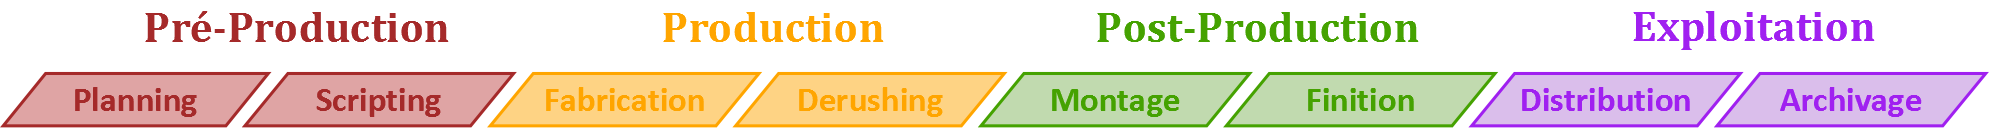
\includegraphics[width=\textwidth]{images/Workflow-Thesis-v0.png}
\caption{La chaîne de production audiovisuelle classique}
\label{img:intro:chaine}
\end{figure}


%%%%%%%%%%%%%%%%%%%%%%%%%
\subsubsection*{Préproduction}\label{sec:preprod}
L'objectif de cette étape est de construire une ébauche du futur document audiovisuel, de manière à prévoir les moyens à engager pour le réaliser. 
On distingue deux phases de préparation, l'écriture ou \e{Scripting} et le \e{Planning} ou planification.

À partir d'une idée, l'écriture du document se déroule en plusieurs étapes où l'on fixe progressivement le message à faire passer ainsi que sa forme audiovisuelle. 
Une fiction par exemple s'écrit à partir d'un résumé de l'histoire, puis on développe les scènes, les personnages, les lieux, les dialogues, etc. jusqu'à arriver à la manière dont cette histoire sera racontée à l'écran. 
On fixe ainsi le type de plan à filmer, les mouvements de caméra, le type de lumière, etc. 
Dans certaines grosses productions, on aura même recours au dessin pour aider à la représentation visuelle.


Toutes ces informations sur le contenu et la forme du futur document audiovisuel servent à estimer le temps nécessaire et les moyens à engager. 
L'estimation du coût d'une production est un élément essentiel pour la production audiovisuelle. 
En effet, dès le départ le producteur doit estimer la rentabilité du futur document afin de voir quels moyens il peut engager. 
Il s'agit bel et bien d'investissement, parfois très lourd, surtout en comparaison avec d'autres industries culturelles – musique, littérature, radio, presse – à l'exception récente du jeu vidéo. 
Contrainte budgétaire et forme esthétique sont donc en négociation dans cette première étape.


%%%%%%%%%%%%%%%%%%%%%%%%%
\subsubsection*{Production}
Une fois l'ébauche et les moyens déterminés, la production vise à réaliser chaque partie du document une à une puis à les assembler en un montage cohérent.

La phase de \e{Fabrication} consiste à capter du réel que l'on a mis en scène. La captation d'un évènement est réalisée grâce à des appareils d'enregistrement (caméra, microphones, etc.). 
La mise en scène du réel se construit à partir d'un ensemble de techniques, d'équipements et d'accessoires (lumière, costume, décors, maquillage, etc.) qui permettent d'obtenir l'image et le son souhaités. 
La technique est ainsi mobilisée dans un objectif esthétique. 
Dans le cas d'une fiction, la fabrication du contenu se fait en fonction du planning de mobilisation des personnes et des équipements plutôt que suivant l'ordre chronologique de l'histoire. 
On regroupe ainsi le tournage des scènes dans tel lieu ou avec tel équipement afin de réduire les coûts. Au final, la fabrication
produit des séquences vidéo et audio qu'il s'agit ensuite de redécouper pour mieux les assembler.

La phase de \e{Derushing} consiste à examiner les séquences réalisées pendant la fabrication et à les trier en vue de faciliter le montage. 
Par exemple, le tournage d'une fiction produit des séquences vidéo comprenant plusieurs prises d'une même scène et souvent des séquences captées par des caméras ayant des angles de prise de vue différents. 
Il faut donc redécouper les séquences en prises puis regrouper les prises d'une même scène. 
Le montage se fera d'autant plus facilement qu'on saura également identifier la qualité et les avantages de chaque prise d'une même scène.


%%%%%%%%%%%%%%%%%%%%%%%%%
\subsubsection*{Postproduction}
Lorsque le contenu audiovisuel est fabriqué et trié, il reste à le structurer en un document et à le conditionner en fonction de sa future exploitation.

La phase de \e{Montage} consiste à agencer des petites séquences de vidéo et d'audio pour construire la structure du document audiovisuel.
L'agencement des plans, leur durée et la transition entre ces plans constituent les ressorts esthétiques propres à l'audiovisuel. 
Ils participent à la transmission du message en ceci qu'ils servent de raccord entre les plans, comme le souligne le réalisateur \pc{Sergueï Mikhaïlovitch Eisenstein}\footnote{L'origine de cette fameuse citation est assez obscur, on la retrouve dans de nombreux documents, dont cet article --\cite{Montage et Réalisme}-- datant des années 60 et extrait de la revue québecoise \gui{Séquence : La revue du cinéma}.} :

\begin{cico}
Le montage est l 'art d'exprimer ou de signifier par le rapport de deux plans juxtaposés de telle sorte que cette juxtaposition fasse naître l'idée ou exprime quelque chose qui n'est contenu dans aucun des deux plans pris séparément. L'ensemble est supérieur à la somme des parties.
\end{cico}

Après le montage, une phase de \e{Finition} est nécessaire pour intégrer d'autres ressources au document en fonction de sa distribution. 
Pour une diffusion antenne d'un reportage, on ajoute le logo de la chaîne de télévision, un jingle, le nom des intervenants ou des titres, etc. 
Une diffusion sur DVD nécessitera l'ajout des conditions
légales d'usages, l'intégration d'un menu de navigation, etc. 
La distribution détermine également un format d'encapsulation (.avi, .mkv, .ogg etc.) et un encodage du contenu audiovisuel (MPEG-2, H.264, MPEG-4, theora vorbis etc.). 
Le résultat de cette phase de post-production est de fournir des documents prêts à l'usage et dans certains cas plusieurs variantes pour chacun des modes de distribution envisagés.


%%%%%%%%%%%%%%%%%%%%%%%%%
\subsubsection*{Exploitation}
Une fois le document achevé, on valorise sa construction par une distribution auprès d'une audience ainsi qu'un archivage qui permettra de le réutiliser ultérieurement.

La phase de \e{Distribution} consiste à rendre le document matériellement accessible à une audience. 
Il s'agit d'un transfert qui peut faire l'objet d'une transaction commerciale ou s'appuyer sur d'autres types de modèles économiques (publicité entre autres). 
La nature du transfert varie et porte à la fois sur les modalités d'accès au contenu et les droits d'usages.

La phase d'\e{Archivage} consiste le plus souvent à stocker le contenu diffusé afin de pouvoir le réutiliser tel quel plus tard, soit en le rediffusant, soit en le vendant à un autre diffuseur. 
C'est aussi généralement la phase où l'on construit, récupère et attache des descriptions du contenu au document audiovisuel. 
En effet, l'archivage n'a de sens que s'il permet de retrouver, voire redécouvrir, les documents archivés.
\ciel{Au plan économique, un film est un bien informationnel, d'expérience, caractérisé par une très forte densité d'informations. Son exploitation s'organise autour de versions différentes, distribuées sur des marchés distincts par des acteurs spécialisés.} (\cite{Blanc2006}).%Gilles Le Blanc - Innovations numériques, distribution et différenciation  : le cas de la projection numérique dans le cinéma.




%<TODO
%TODO>
\subsection{Documents et vocabulaire de la production}\label{sec:docvoc}
\e{
Dans cette section, nous présentons des définitions utilisées dans le milieu professionnel et tirées du \gui{Dictionnaire technique du Cinéma (\cite{Pinel2008})} afin de présenter les principaux documents et le vocabulaire utilisé pendant la phase de préproduction. 
Il s'agit ainsi de mettre en exergue la manière dont se construit une description textuelle de l'objet audiovisuel en devenir ainsi que le vocabulaire utilisé pour faire cette description.}
% Des éléments qui nous serviront à mieux cerner les problèmes qui se posent à la production audiovisuelle.

\paragraph{La notion de plan}
La notion de plan peut se présenter de diverses manières suivant le point de vue adopté. 
Du point de vue technique, il s'agit d'une série d'images (ou photogrammes) qui sont enregistré par un appareil de capatation (une caméra) au cours d'une même prise de vue : \ciel{série de photogrammes enregistrés au cours d'une même prise} (\cite{Pinel2008}).
Il s'agit donc de l'enregistrement qui est effectué entre le moment où l'on presse sur le bouton pour lancer et celui où l'on arrête l'enregistrement.
Cette définition, certes robuste, ne permet pas pour autant de caractériser les plans ou de les comparer entre eux. 
Ainsi, on s'intéresse au point de vue de l'écriture filmique et de la réalisation qui considère non seulement l'action d'enregistrement, mais également la manière dont il est effectué : 

\ciel{
Fragment de temps et d'espace enregistré d'un seul tenant, selon un point de vue déterminé, et donnant à la projection le sentiment de la continuité d'une même \e{image en mouvement}.} (\cite{Pinel2008})

Cette définition complète la précédente en considérant le rapport au sujet (le point de vue) et la temporalité du plan et son rapport à un ensemble d'autres plans (la continuité). 
Elle permet d'envisager les plans comme des éléments de base que l'on assemblera ensuite pour construire un objet audiovisuel : 

\ciel{
La notion de plan est apparue [\dots] lorsqu'on a abandonné le point de vue unique du tableau pour envisager le sujet sous différents angles et à différentes distances et lorsque, par la grâce du montage, on a mis en relation ces plans entre eux.
[\dots]
Si le photogramme représente l'unité technique de la prise de vues, la scène et la séquence les unités narratives de l'oeuvre cinématographique, le plan est la cellule fondamentale de l'écriture du film, de sa préparation jusqu'à la copie standard.} (\cite{Pinel2008})

Dans cette citation, on voit aussi émerger l'idée qu'il existe différents niveaux d'analyse dans l'objet audiovisuel : 
\begin{liste}
	\item un \g{niveau technique} avec le photogramme mais également le pixel dans le numérique.
	\item un \g{niveau narratif} avec la scène (unité de temps et de lieu dans l'histoire) et la séquence (suite de scènes constituant une action dramatique autonome ou distincte).
	\item \g{un niveau dont le plan est l'unité de base qui sert tout au long de la chaîne de production}. 
	On parle d'unité, car il s'agit du résultat de base d'une prise de vue, c'est-à-dire de la fabrication (production) de l'objet audiovisuel. 
	La pré-production, étape de préparation du tournage, utilise donc naturellement cette unité. 
	De même, le montage consiste à organiser ces plans pour former un ensemble cohérent, quitte à les ajuster (raccourcir, allonger, modification du cadrage etc.). 
	Ainsi, il semble que cette unité servent non seulement d'unité de travail de référence pour la chaîne de production\footnote{La production sonore d'un objet audiovisuel ne s'organise pas forcément de la même manière que celle de la production de l'image. Néanmoins, par la force des choses, la construction de l'image prime bien souvent sur celle du son et son unité de base sert donc de référence même pour la production sonore.}, mais également du premier niveau signifiant propre à l'audiovisuel (l'image seul pouvant être rattaché à la photographie).
\end{liste}

Ces distinctions nous permettent de définir le plan selon les caractéristiques suivantes : 
\begin{liste}
	\item \g{l'échelle relative du cadre par rapport au(x) sujet(s)} (personnages, objets etc.).
	C'est ce qui permet de définir un ensemble de \gui{valeurs de plan}, gros plan, plan américain etc. que nous définirons par la suite.
	
	\item \g{l'angle de la prise de vue} (plongée, contre-plongée, cadre incliné etc.)

	\item \g{le mouvement de la caméra} et d'autres paramètres de son objectif (panoramique, travelling, rotation, zoom, focale, focus etc.)

	\item \g{l'articulation des plans entre eux}, d'une part en terme de durée, mais aussi en terme de transition et d'impression de continuité entre les plans. 
	Par exemple, il existe des règles de cadrage et de montage pour aider les spectateurs à situer les personnes sur un plateau\footnote{La règle des 180° oblige ainsi à maintenir les mêmes relations est-à-gauche/droite-de entre les personnes, de manière à ce que le spectateur puisse se souvenir des positions des interlocuteurs sur un plateau. En inversant ces relations topographiques, on donne l'impression au spectateurs que les personnes ont échangé leurs places alors que c'est juste la caméra qui a changé de point de vue. Il s'agit donc d'une règle très importante pour assurer la continuité et la compréhension du spectateur.}.
\end{liste}


\paragraph{Valeurs de plan utilisées dans un script}
La valeur de plan est un des éléments le plus utilisé pour distinguer les plans entre eux, notamment au moment de l'écriture. 
Plutôt que de préciser les paramètres optiques de la caméra (considérés comme des détails très difficile à préciser à l'avance), le réalisateur préfère parler d'un type de plan pour donner une idée générale de l'image à obtenir. 
Le Tableau \ref{tab:vplans} présente les principales valeurs de plans utilisées par les professionnels, avec leur abréviations et leur(s) dénomination(s) anglaise(s) tandis que la Figure \ref{img:intro:plans} en propose une illustration.

\begin{table}[ht!]
   \begin{center}
		\begin{tabularx}{\textwidth}{|p{100pt}|X|p{100pt}|}
		   \hline
	\pc{Dénomination française} & \pc{Défintion} & \pc{Dénomination anglaise} \\ \hline\hline
 	\g{très gros plan (t.g.p.)} & plan cadrant une partie du visage, un détail du corps (un oeil, une bouche, un doigt etc.) ou le détail d'un objet. & extreme close-up, e.c.u. ; big close-up, b.c.u.\\ \hline

 	\g{gros plan (g.p.)} & plan isolant un visage, généralement cadré à la hauteur du noeud de cravate, ou un autre détail du corps (plan de détail ; insert), voire \e{tout ou partie d'un petit objet}. & close-up, c.u.\\ \hline

	\g{plan rapproché} & plan cadrant le(s) personnage(s) au niveau de la taille (plan rapproché taille, p.r.t.) ou de la poitrine (plan rapproché poitrine, p.r.p.). & medium close-up, m.c.u.\\ \hline
	
	\g{plan ceinture} & plan coupant les personnages au niveau de la ceinture & belt shot\\ \hline 

	\g{plan américain} (p.a.) & plan coupant les personnages à mi-cuisse & american shot ; medium close-shot, m.c.s.\\ \hline
	
	\g{plan moyen (p.m.) ou plan en pied} & plan présentant le(s) personnage(s) en pied. Il existe également des variations de ce plan qui sont nommées \e{serré} (aussi nommé plan américain large) ou \e{large} et qui font varier légèrement le cadrage. & medium shot, middle-shot, mid-shot, m.s. ; full shot, f.s.\\ \hline
	

	\g{plan de demi-ensemble (p.d.e., 1/2e.)} & plan mettant en place les personnages dans leur milieu en cadrant une bonne partie du décor & medium-long shot, m.l.s.\\ \hline

	\g{plan d'ensemble (p.e.)} & plan cadrant l'ensemble du décor construit & long shot, l.s.\\ \hline
	
	\g{plan de grand ensemble (p.g.e.)} & plan cadrant l'ensemble du décor construit de grande envergure. & very long shot, v.l.s.\\ \hline

	\g{plan général (p.g.)} & plan couvrant un vaste ensemble qui situe le décor construit dans son cadre : le décor dans le décor. & master shot ; extreme long shot, e.l.s\\ \hline 
		\end{tabularx}
		\caption{Valeurs de plans : du plus précis au plus général \label{tab:vplans}}
   \end{center}
\end{table}

% \begin{liste}
% 	\item \g{très gros plan} (t.g.p.) : \ciel{plan cadrant une partie du visage, un détail du corps (un oeil, une bouche, un doigt etc.) ou le détail d'un objet}. [extreme close-up, e.c.u. ; big close-up, b.c.u.]

% 	\item \g{gros plan} (g.p.) : \ciel{plan isolant un visage, généralement cadré à la hauteur du noeud de cravate, ou un autre détail du corps} (plan de détail ; insert), voire \ciel{tout ou partie d'un petit objet}. [close-up, c.u.]

% 	\item \g{plan rapproché} : \ciel{plan cadrant le(s) personnage(s) au niveau de la taille (plan rapproché taille, p.r.t.) ou de la poitrine (plan rapproché poitrine, p.r.p.).} [medium close-up, m.c.u.]
	
% 	\item \g{plan ceinture} : plan coupant les personnages au niveau de la ceinture [belt shot] 

% 	\item \g{plan américain} (p.a.) : \ciel{plan coupant les personnages à mi-cuisse} [american shot ; medium close-shot, m.c.s.]
	
% 	\item \g{plan moyen} (p.m.) ou \g{plan en pied} : \ciel{plan présentant le(s) personnage(s) en pied.} [medium shot, middle-shot, mid-shot, m.s. ; full shot, f.s.]
% 	Il existe également des variations de ce plan qui sont nommées \ciel{serré} (aussi nommé plan américain large) ou \ciel{large} et qui font varier légèrement le cadrage.

% 	\item \g{plan de demi-ensemble} (p.d.e., 1/2e.): \ciel{plan mettant en place les personnages dans leur milieu en cadrant une bonne partie du décor}. [medium-long shot, m.l.s.]

% 	\item \g{plan d'ensemble} (p.e.) : \ciel{plan cadrant l'ensemble du décor construit}. [long shot, l.s.]
	
% 	\item \g{plan de grand ensemble} (p.g.e.) : \ciel{plan cadrant l'ensemble du décor construit de grande envergure}. [very long shot, v.l.s.]

% 	\item \g{plan général} (p.g.) : \ciel{plan couvrant un vaste ensemble qui situe le décor construit dans son cadre : le décor dans le décor}. [master shot ; extreme long shot, e.l.s] 
% \end{liste}
%TODO:source

\begin{figure}[ht!]
\centering
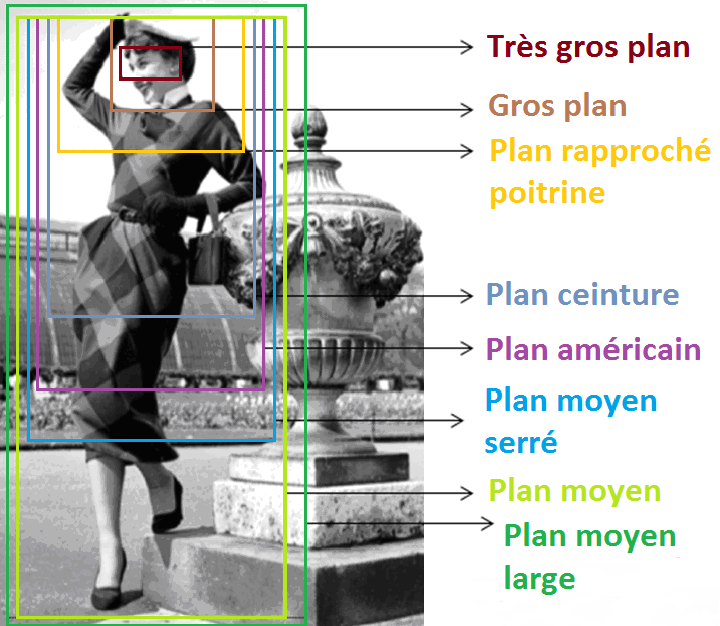
\includegraphics[width=0.4\textwidth]{./images/ValeurPlan-v1.png}
\caption{Différentes valeurs de plan pour le cadrage d'un personnage à l'écran}
\label{img:intro:plans}
\end{figure}


\paragraph{Quelques documents de (pré)production}
%TODO:description + source
La pré-production se repose sur différents types de documents qui permettent de faire émerger progressivement la structure narrative ou documentaire, le découpage en plans et tous les détails de réalisation nécessaire à une bonne préparation du tournage. 
On notera que chacun de ces documents constitue un jalon dans la préparation du projet et que le script, résultat final de cette écriture, constitue une sorte de cahier des charges de l'objet audiovisuel à fabriquer.
\begin{liste}
	\item \g{sujet} : \ciel{matière première du film enrichie et développée lors de la préparation puis mise en forme au cours de la réalisation et du montage.} 
	
	\item \g{synopsis} : \ciel{exposé sommaire en quelques lignes, voire en quelques pages, du contenu dramatique ou documentaire d'un film}. 
	À noter que ce document est également utilisé plus tard dans la chaîne de production, notamment pour être transmis aux journalistes ou aux archivistes.
	De plus, il constitue la première mise en forme narrative du contenu du film, à la différence du sujet qui ne se constitue que de quelques idées directrices. 

	\item en cas d'adaptation d'une oeuvre littéraire en un objet audiovisuel, on développe un \g{traitement} : 
	\ciel{Travail littéraire préparatoire effectué à partir d'une oeuvre pré-existante ou d'une oeuvre originale pour assurer sa transmutation en termes cinématographiques.}

	\item lorsqu'on développe un objet audiovisuel original, à défaut de traitement on peut parler de \g{scénario} :
	\ciel{description de l'action d'un film épousant la forme \e{littéraire} du récit, rendant compte des articulations narratives et comportant une ébauche des dialogues, quelquefois la description plus précise de certaines scènes-clefs.}

	\item lorsque le besoin de préciser encore la construction de la narration, les auteurs peuvent construire une \g{continuité (dialoguée)} : \ciel{étape de la préparation écrite du film qui permet d'enrichir le traitement en développant chronologiquement les fragments d'action, en mettant au point le détail de chaque scène et en précisant le dialogue.}

	\item \g{plan de tournage} : \ciel{ultime travail de préparation effectué par le réalisateur avant le tournage. Il consiste à fragmenter la continuité en unités cinématographiques de temps et d'espace : les plans.}

	\item \g{script} : \ciel{dernière mouture du scénario, guide complet du tournage}.La Figure \ref{img:intro:script} présente un exemple de script extrait d'un film récent écrit et réalisé par Quentin Tarantino.
\end{liste}

\begin{figure}[ht!]
\centering
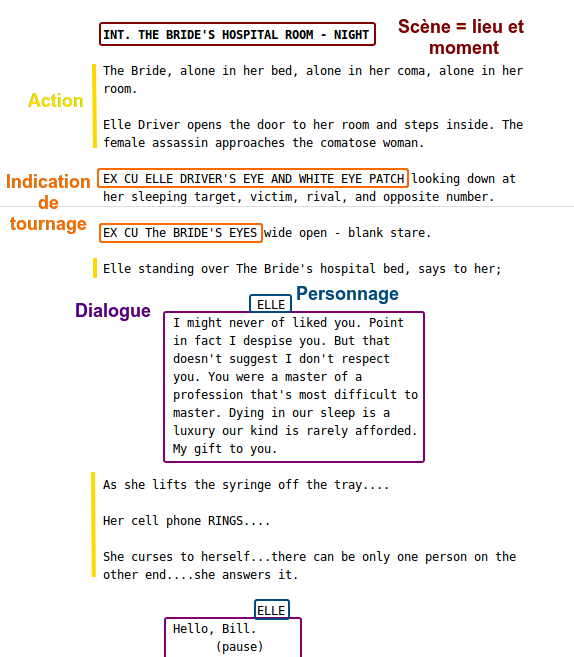
\includegraphics[width=0.7\textwidth]{images/ScriptExample-v1.png}
\caption{Extrait du script de Kill Bill écrit et réalisé par Quentin Tarantino}
\label{img:intro:script} 
\end{figure}

% des réécritures de documents et des mises à jours qui pourraient être réalisées par des machines, des informations qui pourraient être transmises automatiquement à travers un réseau numérique d'information


% un vocabulaire bien défini qui fait l'objet de nombreux dictionnaires, donc prêt à être formalisé


% des équipes qui sont réduites lors de tournage en extérieur




%%%%%%%%%%%%%%%%%%%%%%%%%%%%%%%%%%%%%%%%%%%%%%%%%%%%%%%%%%%%%%%%%%%%%%%%%%%%%%%%%%%%%%%%%%%%%%%%%%%
\subsection{Besoins Métiers}\label{sec:besoins}
\e{
Face à une numérisation qui fragmente les contenus, une mise en réseau qui facilite la fabrication amateur, intensifie la circulation de ces fragments (\ref{sec:motiv}), la production audiovisuelle rencontre de nouveaux défis qui remettent en jeu son organisation et sa manière de se représenter le monde. 
Ainsi d'une part la fragmentation ne doit pas mettre en péril la cohérence de l'ensemble et d'autre part, la circulation des contenus ne doit pas compromettre l'exploitation future du tout ou des parties. 
L'ouverture d'une chaîne de production à des acteurs tiers implique de clarifier les attendus de chacun. 
Lorsqu'il s'agit de faire fabriquer ou de récupérer du contenu, il devient nécessaire pour le client de décrire la commande de contenu au fournisseur, de même que le fournisseur doit décrire à son client le contenu livré pour faciliter son exploitation. 
Ainsi, on souhaite adjoindre aux contenus des descriptions qui permettent de faciliter leur recherche et leur manipulation.
}


Pour les professionnels de la production audiovisuelle, le défi porte à la fois sur l'organisation de leur chaîne de production et sur la gestion de leurs produits :
\begin{liste}
	\item[(1)] \g{comment transformer la chaîne de production afin de l'ajuster à la diversification des formes de fabrication et de distribution des contenus, mais aussi aux changements dans les pratiques de consommation des audiences ?}

	\item[(2)] \g{comment passer d'une gestion de fichiers à une gestion de contenus audiovisuels considérés comme des objets numériques fragmentés dont il s'agit de garantir l'autonomie dès leur conception et jusque dans leurs différents cadres d'exploitation ?}
\end{liste}

% Problèmes métiers ? Tant que ça ne devient pas une solution, mais des tendances à prendre en compte 

On peut ensuite détailler ces défis en objectifs plus précis :
\begin{liste}
	\item[(1a)] \e{accorder contribution amateur et production professionnelle pour fabriquer ou valoriser du contenu.}

	L'amélioration croissante des capteurs des appareils multimédia ajoutée aux capacités de communication offrent au grand public de plus en plus de manières de participer aux processus de fabrication ou de diffusion des contenus.
	Les possibilités accrues de participation au processus médiatique (participation à l'émission, envoi de contenu, propagation via ses contacts, commentaires etc.) valorisent le spectateur, le contenu et la plate-forme de diffusion (comme d'une certaine manière peut le faire le bouche à oreille).

	De manière générale, l'intégration de contenus externes dans une chaîne de production professionnelle ne s'envisage  qu'à partir d'un certain niveau de qualité du contenu livré.  
	Paradoxalement, dans certains cas les signes d'une production amateur (tremblements, caméra à l'épaule etc.) peuvent être revendiquées comme des marque de style qui suggère une collaboration avec le public ou une proximité avec une réalité éloignée des images diffusées par les médias.
	Ainsi, les professionnels souhaitent encadrer plus ou moins fortement la production amateur par des indications, recommendations, obligations.\\


	\item[(1b)] \e{créer de nouvelles étapes dans la chaîne visant à réutiliser les contenus existants et les adapater à de nouveaux modes de consommation.}

	L'augmentation de l'offre de contenus accessibles aux spectateurs (chaînes, enregistrements, balladodiffusion, vidéo à la demande etc.) se traduit par une mise en concurrence accrue des contenus diffusés par les professionnels.
	Le contrôle de l'offre n'étant plus atteignable, il faut adopter de nouvelles stratégies de valorisation des contenus produits ou diffusés pour maintenir leur visibilité et leur rentabilité. 
	Une autre approche consiste à fournir un service de recommandation aux spectateurs et ainsi rentrer dans une démarche de fidélisation. 

	Par ailleurs, l'augmentation des terminaux de lecture multimédia et leur portabilité offrent de plus en plus d'occasions aux spectateurs de consommer des contenus. 
	Par exemple, les situations de mobilités peuvent impliquer des capacités de transfert diminués, un écran plus petit, des temps de disponibilités plus courts etc.
	Il semble alors que la production doivent évoluer pour fournir de nouveaux formats ou des formes retravaillées de contenus existants.

	Dans tous les cas, cela implique de se consacrer à des tâches d'éditorialisation des contenus pour répondre aux exigences et aux attentes de ces nouveaux modes de consommation.\\
% \end{liste}


% \begin{liste}
	\item[(2a)] \e{gérer l'intégration de contenu externes, les variations d'un même contenu pour les rattacher à un même objet numérique.} 
	% représentation

	L'utilisation de contenus provenant de sources externes de même que la production de multiples variations d'un même contenu augmente le nombre de ressources à gérer. 
	De plus, les relations entre ces différentes ressources nécessitent d'être clarifiées et explicitées dans le système de gestion. 
	% chaîne éditoriale ? 
	
	Il ne s'agit plus simplement de gérer des fichiers mais un ensemble de fichiers et de données qui constituent un ensemble cohérent et fragmenté que l'on nomme un objet numérique. 
	Cet objet doit intégrer à la fois les diverses sources qui le composent mais aussi des variations correspondants aux exploitations visées, des descriptions et tout ce qui permet de garantir son autonomie. 
	Il doit également s'agir d'un objet \e{métier} car son statut, son organisation, sa sémantique correspondent à la vision d'un métier, à la manière dont il pense le monde. 

	% Ainsi, on ne souhaite plus gérer des fichiers mais des objets numériques qui doivent acquérir un statut, une sémantique correspondant à la manière dont les métiers de la production les considèrent.\\
	% qui possède une valeur et une sémantique propre à un contexte d'usage. 	


	\item[(2b)] \e{associer des descriptions aux contenus pour faciliter leur exploitation dans un environnement numérique.}
	% description

	L'augmentation des contenus audiovisuels en circulation, la diversification de leurs modes d'exploitation compliquent la gestion des contenus.  
	Afin de favoriser la réutilisation de ces contenus, il faut pouvoir leur attacher des informations pertinentes pour les professionnels qui les manipulent. 
	La description du contenu peut varier suivant les besoins de chaque métier impliqué dans la chaîne de production. 
	Les opérations n'étant pas les mêmes, les descriptions de ces opérations varient donc également et sont nécessaires pour faciliter la réutilisation du contenu. 
	%de manière à faciliter modalités d'exploitation envisagées  

	Lorsque la réutilisation et production s'entremêlent, il est également nécessaire de construire les descriptions en même temps que le contenu. 
	De cette manière on récupère ou on réévalue l'information à mesure de l'avancée dans la chaîne. 

	Cela nécessite d'informatiser l'étape de pré-production de la chaîne et de modéliser les informations utilisées par les professionnels. 
	%commencer plus tôt, avoir plusieurs niveaux/types de description, raccrocher les bons éléments à la représentation de l'objet numérique
	
	%et embarquent des descriptions explicitant leurs modalités d'exploitation.

\end{liste}

\e{
En guise de synthèse, nous pouvons dire qu'il s'agit de constituer des objets audiovisuels autonomes dans les chaînes de production audiovisuelle. 
Nous précisons ce caractère autonome, car ces objets seront porteurs de leur propre description et associés à des connaissances sur l'organisation de la chaîne de production dans lesquels ils évoluent.
Ainsi, ces objets audiovisuels pourront être (ré)introduits à n'importe quelle étape d'une chaîne de production et fourniront aux contributeurs concernés des informations propres à faciliter leur (ré)utilisation.
}
	% \item \eg{valoriser et éditorialiser les contenus existants pour les rendres plus visibles, plus attrayants auprès des audiences ciblées.}
	% L'augmentation de l'offre de contenus accessibles aux spectateurs (chaînes, enregistrements, balladodiffusion, vidéo à la demande etc.) se traduit par une mise en concurrence accrue des contenus diffusés par les professionnels.

	% Le contrôle de l'offre n'étant plus atteignable, il faut adopter de nouvelles stratégies de valorisation des contenus produits ou diffusés pour maintenir leur visibilité et leur rentabilité. 
	% Une autre approche consiste à fournir un service de recommandation aux spectateurs et ainsi rentrer dans une démarche de fidélisation. 
	% Cela implique de se consacrer à des tâches d'éditorialisation des contenus pour des audiences plus ciblées.
	
	% \item \eg{produire de nouvelles formes de contenus ou adapter les rmes existantes pour satisfaires aux nouveaux modes de distribution/consommation.}
	% L'augmentation des terminaux de lecture multimédia et leur portabilité offrent de plus en plus d'occasions aux spectateurs de consommer des contenus. Par exemple, les situations de mobilités peuvent impliquer des capacités de transfert diminués, un écran plus petit, des temps de disponibilités plus courts etc.
	% Il semble alors s'ouvrir une place pour de nouveaux formats ou des formes retravaillés de contenus existants. 
	% Il s'agit de faire de la production multi-support et d'adapter les contenus en fonction des conditions de distribution et de l'audience visé (réutilisation).
	
	% \item \eg{articuler la contribution amateur avec la chaîne de production professionnelle.}
	% L'amélioration croissante des capteurs des appareils multimédia ajoutée aux capacités de communication offrent au grand public de plus en plus de manières de participer aux processus de fabrication ou de diffusion des contenus.
	% Les possibilités accrues de participation au processus médiatique (participation à l'émission, envoi de contenu, propagation via ses contacts, commentaires etc.) valorisent le spectateur, le contenu et la plate-forme de diffusion.

	% Cependant, il faut être capable d'intégrer ces contributions externes au sein de la production professionnelle en les encadrant plus ou moins fortement, par des indications, recommendations ou des contraintes.

	% \item \eg{gérer les objets audiovisuels dès le début et tout au long de leur cycle de vie.}
	% %
	
	% Une circulation plus importante des contenus implique de trouver un moyen de gérer non plus des fichiers mais des objets numériques qui unifient plusieurs variations d'un même contenu et embarquent des descriptions explicitant leurs modalités d'exploitation.



% numériser => (a) fragmenter + (b) mettre en réseau => (a) besoin de conserver la cohérence de l'ensemble + (b) besoin d'autonomiser pour une future situation d'usage








%%%%%%%%%%%%%%%%%%%%%%%%%%%%%%%%%%%%%%%%%%%%%%%%%%%%%%%%%%%%%%%%%%%%%%%%%%%%%%%%%%%%%%%%%%%%%%%%%%%
% \newpage
\section{Problèmes}\label{sec:prob}



%%%%%%%%%%%%%%%%%%%%%%%%%%%%%%%%%%%%%%%%%%%%%%%%%%%%%%%%%%%%%%%%%%%%%%%%%%%%%%%%%%%%%%%%%%%%%%%%%%%
\subsection{Problèmes métiers}\label{sec:pmetiers}
% Nos champs d'applications sont : 
% Prenant acte des besoins de la production audiovisuelle nous distinguons deux problèmes métiers (1) identifier le(s) niveau(x) de fragmentation et (2) le(s) type(s) de description susceptibles de favoriser la fabrication mixte, la circulation et la réutilisation des contenus.
% Ces problèmes remettent en cause à la fois la représentation classique des contenus et leur description. 
% de manière à faciliter (1) la production mixte amateur-professionnel et (2) leur réutilisation dans de nouveaux contextes d'exploitation.
% l'informatisation du début de la chaîne de production, préproduction 
% l'inscription formelle de l'écriture audiovisuelle ?

\e{
L'objectif central qui se pose à la production audiovisuelle est de constituer des objets audiovisuels autonomes et donc (ré)utilisable à n'importe quel étape de la chaîne. 
Or, dans la chaîne de production classique les programmes n'émergent qu'à la fin de la chaîne et sont gérés d'une pièce. 
Il n'y a pas forcément de place pour les éléments de contenu intermédiaires, et c'est justement à la modélisation de ces fragments que l'on s'attaque. 
Ces fragments doivent devenir des éléments documentaires qui possèdent leur unité propre de même que les objets finis que sont les programmes. 
Une des difficultés réside dans cette articulation entre des fragments et le tout ou l'ensemble que constitue les programmes. 
Par ailleurs, il existe des problèmes sous-jacents à cette fragmentation documentaire : 
}
\begin{liste}
	\item \e{identifier quels niveaux de fragments peuvent prétendre à ce genre de transformation}.
	Si le numérique permet de fragmenter à l'envie, il faut cependant prendre en compte les pratiques du métier pour identifier les niveaux de fragmentation pertinents ou déjà utilisés dans le métier mais non modélisés.
	Par exemple, la prise de vue est le résultat d'une activité de tournage, pour autant elle ne constitue pas un objet éditorial comme peut l'être une interview.
	De plus, il s'agit également de déterminer comment manipuler ces fragments comme des objets à part entière sans compromettre l'articulation de l'ensemble. 
	Par exemple, une interview peut s'intégrer dans un journal télévisé ou bien un reportage dans des versions plus ou moins courtes. 
	Pour autant, il s'agit du fruit d'une même activité, simplement le montage, et donc le résultat, est différent suivant le programme dans lequel l'interview s'insère.\\
	
	\item \e{identifier quelles informations et connaissances doivent être rattachées à ces fragments pour les rendre autonome}.
	D'une manière similaire à la démarche pour les objets entiers, certaines connaissances, notamment relatives au contexte de production, doivent être attachées au fragment pour garantir sa réutilisation et sa cohérence. 
	En reprenant l'exemple de la prise de vue, on peut lui associer le bout de script qui a prescrit ce qu'elle devait montrer. 
	Si l'on pousse encore cette logique, il faut également incorporer le document qui définit le programme pour lequel on a tourné cette prise de vue, la personne qui l'a effectuée, les équipements utilisés etc. 
	Ainsi, on étend la modélisation de l'objet audiovisuel à son contexte de production et tout ce qui renforce les possibilités de recherche, de manipulation, de gestion et de transformation de ces objets. 
	De plus, s'ajoute à cela la question de la collecte de ces informations. 
	En effet, la saisie de ces informations au sein d'un système d'information et leur utilisation par les acteurs de la chaîne n'est pas une simple formalité.
	Ce problème pousse également dans le sens d'une modélisation plus contextuelle, de manière à proposer un environnement de travail adapté et utilisable aux contributeurs de la chaîne.\\
	
	% \item \e{}.
\end{liste}


% Notre problème se situe dans le croisement de la représentation des contenus et la représentation des activités humaines qui construisent, manipulent, éditent, transforment, publient et documentent ces contenus. 
% Cet angle de recherche nous amène donc à considérer non pas le contenu audiovisuel dans son ensemble, une fois terminé et validé, mais la construction de tout ces fragments qui le composent. 
% Il nous faut aussi considérer, non pas seulement le contenu audiovisuel, mais aussi d'autres informations, d'autres documents qui constituent son contexte de production, dans un sens très général. 
% Chaque prise de vue constitue donc un objet à représenter en tant que tel, tout autant que le bout de script qui a prescrit ce que cette prise de vue devait montrer. 
% Si l'on pousse encore cette logique, on peut alors représenter de même le document qui définit le programme pour lequel on a tourné cette prise de vue, la personne qui l'a effectué, les équipements utilisés etc. 
% Ainsi, on étend la représentation du contenu à son contexte de production entendu comme toutes les informations qui renforceront les possibilités de recherche, de manipulation, de gestion et de transformation de ces contenus. 

%%%%%%%%%%%%%%%%%%%%%%%%%%%%%%%%%%%%%%%%%%%%%%%
\subsection{Problèmes scientifiques}\label{sec:scien}
Au fur et à mesure que la circulation des contenus s'intensifie, il y a un besoin grandissant de faciliter l'échange d'information tant à la fois sur le plan informatique, que sur le plan humain. 
De plus, l'ouverture de la chaîne de production à de nouveaux contributeurs (amateurs et professionnels) ne fait qu'accentuer la disparité des connaissances et des systèmes utilisés. 
Afin de construire une compréhension commune à tous les contributeurs au cycle de vie, on fabrique un modèle conceptuel capable d'intégrer et de mettre en relation leurs connaissances. 
Il s'agit là d'un apport par rapport à la situation existante où le consensus n'existait pas, ou alors de manière éphémère, locale au sein d'une équipe.
L'objectif est de fluidifier les échanges d'information et de contenus en formalisant les connaissances utilisées pour :
\begin{problemes}{LightGoldenrodYellow}
\begin{liste}
% modéliser tous les objets de la chaîne de production audiovisuelle
	\item[(A)] \g{modéliser les objets construits au fil de la chaîne de production audiovisuelle}.
	\item[(B)] \g{modéliser les connaissances sur ces objets} (descriptions, contexte de production, contribution au cycle de vie).
	% \item[(B)] décrire les objets audiovisuels
	% \item[(C)] représenter la contribution de chacun des acteurs au cycle de vie des objets audiovisuels
\end{liste}
\end{problemes}

\e{
Ainsi, notre problème de recherche général s'articule autour de la modélisation des connaissances et des informations que les contributeurs construisent, utilisent, échangent au cours du cycle de vie des objets audiovisuels. 
Cette modélisation constitue une première étape dans la mise en place d'un système d'information servant à mieux gérer les objets audiovisuels et médier la communication entre systèmes informatiques tout autant qu'entre contributeurs humains.
Après avoir numérisé les contenus audiovisuels, on souhaite transformer chaque élément les composant en objet documentaire et documenter leur cycle de vie.\\}



\g{(A)} Le problème est d'organiser la gestion des objets audiovisuels en proposant une modélisation capable de faciliter leur identification, leur manipulation et leur réutilisation tout au long de leur cycle de vie. 
En particulier,	l'objet audiovisuel professionnel est produit de manière collective, chaque contributeur apportant un élément à l'ensemble. 
Ces contributions doivent donc pouvoir être identifiées comme appartenant à un ensemble, de même que chaque élément doit pouvoir être considéré pour soi afin d'être intégré dans un autre ensemble (réutilisation).

Pour cela on adopte une représentation des différents niveaux d'abstraction des objets audiovisuels numériques de façon à rétablir les liens entre les différentes versions ou copies d'un même contenu, quelque soit la nature des variations entre elles (encodage, format d'encapsulation, montage, finition, langue etc.).
La distinction entre différents niveaux de modélisation (technique, esthétique, éditorial etc.) doit permettre de construire une représentation dynamique de l'objet audiovisuel qui suit l'avancement du processus de production.\\
% La distinction entre différents niveaux de modélisation (technique, esthétique, éditorial etc.) doit permettre de construire une représentation de l'objet audiovisuel au fur et à mesure de l'avancement du processus de production.\\


\g{(B)} Le problème est d'attacher plusieurs types de connaissances aux objets audiovisuels de manière à les rendre autonomes dans leur circulation et leur réutilisation. 
Afin de faciliter l'échange d'information et la réutilisation des objets audiovisuels entre différents contextes, il faut modéliser des connaissances sur ces objets qui sont parfois déjà existantes mais non formalisées, ou bien qu'il faut rendre compréhensibles.
En effet, l'échange d'informations dans la production audiovisuelle est primordial et s'effectue entre métiers ou organisations différent(e)s, voire avec des amateurs. 
En particulier, on souhaite s'appuyer sur le vocabulaire de l'écriture filmique utilisé dans des documents de préproduction pour spécifier les résultats attendus de la production.
L'information contenue dans ces documents est importante mais repose sur des conventions plus ou moins tacites qu'il faut expliciter pour les professionnels, expliquer pour les amateurs.
La formalisation de ces éléments devra donc pouvoir être lu et modifié tout au long du cycle de vie des objets audiovisuels par tout types de contributeurs.

% échange d'info, adaptation par l'explicitation du vocabulaire et la contribution au cycle de vie
La formalisation de l'écriture filmique permettra d'adapter la présentation de l'information en fonction des connaissances, de l'implication du contributeur dans la chaîne (rôle, tâche, niveau de compétences etc.), de son référentiel professionnel ou linguistique. 
Il s'agit alors d'établir des correspondances entre les connaissances connues par le lecteur d'une information et celles utilisées par la personne qui l'a exprimée.
Ainsi, d'une part on explicite l'expression de l'information, ce qui permet l'adpatation, et facilite son interprétation ultérieure.
Le processus prend tout son sens lorsqu'il s'agit de traduire un concept de la réalisation audiovisuelle pour guider un amateur dans son tournage.
% Par exemple, l'action écrite par l'auteur et transformé en scène par le réalisateur, doit ensuite être tourné un caméraman, des acteurs etc. 


% réutilisation, attachement des connaissances pertinentes pour manipuler ou exploiter chaque fragment ou l'objet en entier
De plus, les descriptions utilisées, en plus de permettre de spécifier le résultat attendu de la production, doivent permettre de faciliter la recherche, la manipulation et la réutilisation des objets audiovisuels.
Pour cela, il faut articuler ces connaissances aux objets et aux fragments qui les composent. 
Le vocabulaire de l'écriture filmique sera également précieux, puisqu'il nous donne une unité de base, le plan, ainsi que ses caractéristiques qui permettent de le distinguer des autres. 
La recherche dans des dépôts de contenus se fera ainsi de manière similaire à la commande de contenu à d'autres contributeurs, qu'ils soient professionnels ou amateurs.



% Il s'agit donc de définir un modèle de description susceptible d'être utilisé par les contributeurs professionnels ou amateurs, à toutes les étapes de la chaîne de production. 


% Afin de décrire les contenus, on souhaite s'appuyer sur le vocabulaire de l'écriture audiovisuelle utilisé dans les différentes étapes de la chaîne et notamment dès la préproduction. 
% Cette écriture repose sur un vocabulaire des techniques de réalisation audiovisuelle (prise de vue, transition, composition de l'image etc.) renvoyant à des effets largement connus dans le milieu de l'audiovisuel et chez les cinéphiles. 
% L'écriture est utilisée avant la fabrication du contenu pour la spécifier, puis pendant la fabrication pour enregistrer les différences. 
% Une formalisation de ce vocabulaire permettrait de construire une description textuelle d'un contenu à partir d'une description objective de la réalisation (réglages des appareils, position des acteurs etc.).\\



% \g{(C)} Le problème est de représenter et faciliter l'échange d'information entre des contributeurs hétérogènes dans leurs connaissances et leur implication dans la chaîne de production.
% Une première diffculté réside dans l'articulation entre les connaissances des contributeurs qui expriment l'information et ceux qui l'interprèteront.
% La seconde diffculté consiste dans l'articulation des représentations du cycle de vie, de l'objet audiovisuel et des descriptions qui leurs sont associées. 
% En effet, chaque contributeur peut participer à la constitution d'informations associées au contenu en cours de sa production.
% Ces informations varient en fonction de l'implication du contributeur dans la chaîne (rôle, tâche, niveau de compétences etc.). 
% De plus, les informations construites à un moment sont susceptibles d'être utilisées plus tard dans la chaîne, par un contributeur ne partageant pas forcément les mêmes connaissances ou le même référentiel professionnel ou linguistique.

% On cherche alors à réaliser une adaptation de la forme d'expression de ces informations afin de faciliter le déroulement du processus de production. 
% Dans un premier temps, on explicite les connaissances utilisées par un premier utilisateur pour exprimer une information. 
% Ensuite, on établit une correspondance avec les connaissances connues d'un autre utilisateur et on adapte au besoin la forme de d'expression de cette information pour faciliter son interprétation. 
% L'adpatation qui en résulte prend tout son sens lorsqu'il s'agit de traduire un concept de la réalisation audiovisuelle pour guider un amateur dans son tournage.


%%%%%%%%%%%%%%%%%%%%%%%%%%%%%%%%%%%%%%%%%%%%%%%
% \section{Positionnement Disciplinaire (n,i)}\label{sec:posd}
% [Ingénierie des connaissances ; Media Asset Management ; Gestion électronique de Documents ; Ingénierie documentaire]
% ingénierie des connaissances (représentation des connaissances) ingénierie des inscriptions numériques de connaissances, dont les documents
% ingénierie documentaire (modélisation des documents propres à la production audiovisuelle)
% indexation et gestion des connaissances (description des contenus audiovisuels)
% la ged s'occupe de la gestion de documents, nous proposons de gérer des fragments de documents, de gérer leur construction en plusieurs étapes, par plusieurs acteurs et dans le cadre de différentes missions.

% Pour définir cet ensemble d'informations qui forment le contexte de production, nous nous sommes appuyés sur les partenaires du projet MediaMap. 



% des réécritures de documents et des mises à jours qui pourraient être réalisées par des machines, des informations qui pourraient être transmises automatiquement à travers un réseau numérique d'information
% un vocabulaire bien défini qui fait l'objet de nombreux dictionnaires, donc prêt à être formalisé
% des équipes qui sont réduites lors de tournage en extérieur

% à mettre dans le pos. disciplinaire, comment on aborde les problèmes posées
% [Nous avons ainsi dégagé plusieurs perspectives métiers qui nous ont servi de guide pour identifier les échanges d'informations les plus importants ainsi que le vocabulaire utilisé pour les exprimer. 
% Chacune de ces perspective possède un objectif propre et des spécificités, cependant il apparaît qu'un langage commun est utilisé par tous les acteurs de la production. 
% En se concentrant sur la description d'un contenu existant ou à venir, ce langage permet à ces acteurs de communiquer entre eux. Le réalisateur qui spécifie un attendu dans son script, les caméraman qui réalisent le cadrage, les opérateurs lumières etc. 
% Tous utilisent ce langage pour imaginer le résultat à produire et en déduire les gestes à opérer. 
% Les usages n'étant jamais complètement figé, chaque organisation développe ses propres idiomatismes de langage. 
% Dans ce cas, la collaboration entre organisations impliquent de pouvoir réaliser des ajustements dans l'expression de la description du contenu. 
% De même, la collaboration avec des contributeurs amateurs soulève un problème de compréhension de ce langage (et donc de l'attendu) mais aussi de connaissances des gestes à opérer (pour produire le résultat attendu).
% Ainsi, à mesure que la circulation des contenus s'intensifie, que les besoins de collaboration augmentent, naît un besoin grandissant d'explicitation des échanges d'information afin de dégager une vue d'ensemble de la chaîne de production, de ses acteurs, de leurs interactions, de leurs produits. 

% Notre proposition consiste à modéliser ces éléments et à en informatiser l'accès de manière à fluidifier les échanges de contenus et faciliter la compréhension des informations afférentes.] 


% \cleardoublepage





%%%%%%%%%%%%%%%%%%%%%%%%%%%%%%%%%%%%%%%%%%%%%%%%%%%%%%%%%%%%%%%%%%%%%%%%%%%%%%%%%%%%%%%%%%%%%%%%%%%
%%%%%%%%%%%%%%%%%%%%%%%%%%%%%%%%%%%%%%%%%%%%%%%%%%%%%%%%%%%%%%%%%%%%%%%%%%%%%%%%%%%%%%%%%%%%%%%%%%%
\part*{État de l'art}
\addcontentsline{toc}{part}{État de l'art}
%%%%%%%%%%%%%%%%%%%%%%%%%%%%%%%%%%%%%%%%%%%%%%%%%%%%%%%%%%%%%%%%%%%%%%%%%%%%%%%%%%%%%%%%%%%%%%%%%%%
%%%%%%%%%%%%%%%%%%%%%%%%%%%%%%%%%%%%%%%%%%%%%%%%%%%%%%%%%%%%%%%%%%%%
%%%%%%%%%%%%%%%%%%%%%%%%%%%%%%%%%%%%%%%%%%%%%%%%%%%%%%%%%%%%%%%%%%%%
%%%%%%%%%%%%%%%%%%%%%%%%%%%%%%%%%%%%%%%%%%%%%%%%%%%%%%%%%%%%%%%%%%%%
%%%%%%%%%%%%%%%%%%%%%%%%%%%%%%%%%%%%%%%%%%%%%%%%%%%%%%%%%%%%%%%%%%%%
\chapter{Outils de modélisation}\label{c:omod}


% pourquoi on parle de SOC ? Parce qu'on souhaite représenter des objets audiovisuels, leur production, leur description et que ceci ne peut se faire sans une représentation du vocabulaire utilisé dans la production audiovisuelle. 

Dans le cadre de la production audiovisuelle collaborative, qui implique à la fois des amateurs et des professionnels, un des enjeux que nous avons noté (\ref{sec:scien}) est de rendre plus compréhensible l'échange d'informations entre contributeurs. 
D'une part, nous avons des practiciens professionnels utilisant un ou plusieurs vocabulaires métiers suffisamment définis pour que l'on puisse en faire des dictionnaires (\cite{Journot2008}; \cite{Pinel2008}). 
Ces personnes font usage de la langue d'une manière précise, régie par des conventions et portée par une conception de la production audiovisuelle et de ses objets, que l'on suppose stabilisée, au moins localement (au sein d'un même pays, d'une même école de pensée, organisation, équipe etc.).
Toutefois, on s'attend à des variations dans les usages de la langue, au même titre que l'on suppose qu'il existe des variations entre pratiques des gens du métiers.
Cependant, il semble qu'il s'agit seulement de variations et qu'il soit possible alors d'identifier les éléments communs et distincts.

D'autre part, les amateurs, quant à eux, n'ont pas le support de ces conventions travaillées au quotidien.
Ils sont, au mieux, des intermittents éclairés qui ont saisi le sens d'éléments de langage propres aux métiers (par des lectures, des rencontres, des formations etc.). 
Il faut donc supposer qu'il y a tout à expliquer à ces amateurs, plutôt que de parier sur leur compréhension innée des métiers de la production audiovisuelle.
En particulier s'il s'agit de demander du contenu à des amateurs sous la forme d'un script de tournage, il faudra alors trouver un moyen d'expliciter cette commande et d'expliquer ou d'assister sa réalisation. 

Ainsi, l'écart entre collaborateurs (qu'ils soient tous professionnels, ou un mélange d'amateurs et de professionnels) peut se situer sur différents niveaux : 
\begin{liste} 
	\item au niveau du vocabulaire métier, comme les mots utilisés dans le script pour désigner tel ou tel type de plan etc. 
	Dans le cas d'amateurs, il faut supposer que ces mots sont inconnus ou méconnus ; dans le cas de professionnels, on préfèrera expliciter le vocabulaire afin d'éviter toute confusion. 
	
	\item au niveau des connaissances et de la manière de conceptualiser le métier, le cycle de production et ses objets. 
	Là encore, un amateur ne connaît pas ou très peu les détails classiques des méthodes de production professionnelle. 
	De plus, la production audiovisuelle étant organisée en projets distincts, les méthodes peuvent fortement varier entre la production d'un documentaire et d'une émission de variétés. 
	Chaque genre, chaque équipe aura donc ses propres objets, ses propres méthodes qu'il faut alors expliciter aux autres professionnels pour s'assurer de leur collaboration. 

	\item sur le plan pratique, il faut également remarquer que les compétences peuvent également varier fortement entre métiers, suivant les genres de production audiovisuelle. 
	Ainsi, en plus d'expliciter les échanges d'informations, il serait également souhaitable de proposer une assistance aux collaborateurs amateurs ou professionnels pour s'assurer que le résultat produit correspond bien à l'attente initiale. 	
\end{liste}


Nous présentons dans une première section un exemple de commande de tournage qui illustre ces différents écarts en impliquant des communautés d'amateurs et de professionnels (\ref{sec:cdcf}). 
Ce scénario d'usage nous permet de préciser les besoins en modélisation exprimées précédemment (\ref{sec:prob}).
Notamment, il apparaît nécessaire de représenter à la fois la ou les conceptualisation(s), le(s) vocabulaire(s) utilisé(s) ainsi que les résultats attendus par les acteurs de la chaîne de production audiovisuelle. 
Ainsi, nous nous intéresserons à l'utilisation de divers Systèmes d'Organisations de Connaissances (SOC, \cite{Zacklad2010}) pour mettre en place un partage d'information normalisée. 
Après un retour sur les définitions principales que nous utiliserons, nous examinerons les langages, modèles et normes existants qui permettent de représenter des SOC (\ref{sec:defs}).
La distinction entre terminologie et ontologie nous nous permet de détailler le fonctionnement d'une méthode de construction d'ontologie différentielle (\ref{sec:construction}).
Enfin, nous présenterons les langages permettant de représenter ces SOCs (\ref{sec:mods}). 

%Dans une seconde partie, nous examinerons les modèles de l'audiovisuel existants.




%%%%%%%%%%%%%%%%%%%%%%%%%%%%%%%%%%%%%%%%%%%%%%%%%%%%%%%%%%%%%%%%%%%%
%%%%%%%%%%%%%%%%%%%%%%%%%%%%%%%%%%%%%%%%%%%%%%%%%%%%%%%%%%%%%%%%%%%%
\section{Cahier des charges fonctionnel (n)}\label{sec:cdcf}


%%%%%%%%%%%%%%%%%%%%%%%%%%%%%%%%%%%%%%%%%%%%%%%%%%%%%%%%%%%%%%%%%%%%
\subsection{Scénario de commande de tournage}\label{sec:scenar}
Considèrons comme cas d'étude une commande de tournage en vue de réaliser des reportages sur des évènements culturels de type concert ou opéra. 
Il met en jeu trois communautés en collaboration :

\begin{itemize}
	\item la RTBF (Radio Télévision Belge Francophone) établit des commandes de contenu dans un jargon métier propre. Son objectif est d'externaliser dès que possible la réalisation de la commande. Cela implique une compréhension commune sur le contenu à réaliser qui passe par un accord sur la manière de décrire la commande. 
	
	\item le contenu commandé est tourné soit par la VRT (Radio-Télévision Flamande) qui utilise un jargon différent de la RTBF, soit des amateurs qui ne connaissent pas les concepts de la réalisation audiovisuelle. Dans le premier cas, la conceptualisation est commune, seuls les termes changent. Dans le second cas, il s'agit d'expliquer et d'illustrer les concepts utilisés \\
\end{itemize}

Le développement d'une application d'assistant de tournage pour guider les amateurs paraît souhaitable pour amener le contenu filmé à un niveau de qualité exploitable. 
Il faut cependant faire la distinction entre les propositions de dépôt spontané de contenu (comme le pratique une chaîne d'information telle que BFM\footnote{La rubrique témoins BFM permet à un utilisateur de déposer des photos ou vidéos sur le site. 
Après modération, le contenu est diffusé et peut même faire l'objet d'une vente. Voir http$:$//temoins.bfmtv.com/}) et les appels à contribution où le professionnel passe commande auprès d'amateurs en détaillant ses exigences. 

Dans ce dernier cadre, on souhaite fournir un plan de tournage au caméraman afin de guider sa prise de vue. 
Le plan de tournage est construit à partir de recommandations rédigées par un réalisateur (position, cadrage, lumière, etc.) utilisant un vocabulaire métier. 
L'originalité de l'application est d'adapter l'information présentée au caméraman suivant ses capacités (amateur, professionnel) ou son employeur si c'est un professionnel travaillant dans une tierce organisation. 
On suppose ainsi que malgré quelques variations dans le vocabulaire utilisé, les professionnels de l'audiovisuel utilisent les mêmes concepts pour décrire le contenu. 
Par exemple, la notion de cadrage fait appel à des concepts de valeurs de plan indiquant la portion visible d'un personnage à l'écran (voir Figure \ref{img:intro:script}, page \pageref{img:intro:script}).
Un \textit{plan américain} indique ainsi que le personnage principal est cadré de la tête jusqu'au dessus des genoux. 
Le terme est utilisé en Europe en rappel à son emploi caractéristique dans les films américains des années 1910-1940, notamment dans les westerns où il permettait de montrer l'ensemble du pistolet à la ceinture des personnages\footnote{Roger Boussinot, l'Encyclopédie du Cinéma, Bordas.}. 
Ce cadrage est aussi appelé \textit{plan 3/4} et en anglais 3/4 shot, medium-long shot ou american shot pour traduire l'expression popularisée en Europe. 
Si le terme utilisé varie suivant le lieu et la littérature de référence, la définition de ce type de cadrage est sans équivoque. 

%=============
% \begin{figure}[htb]
% \centering
% 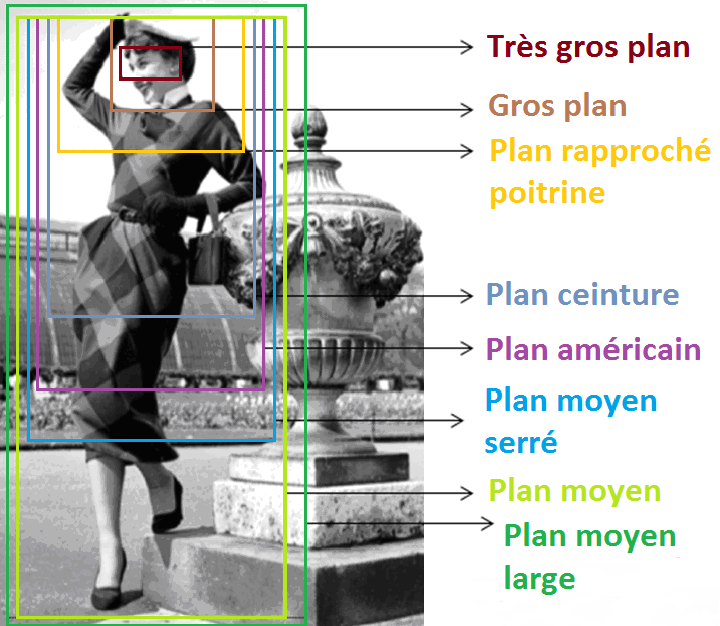
\includegraphics[width=0.5\textwidth]{./images/ValeurPlan-v1.png}
% \caption{Différentes valeurs de plan pour le cadrage d'un personnage à l'écran}
% \label{fig:cadrage}
% \end{figure}
%=============

Les amateurs quand à eux ignorent ces concepts et n'ont pas été initiés à ces pratiques. Ils ont donc besoin d'explications et d'illustrations pour comprendre les recommandations du réalisateur. 
Dans le cas du cadrage, une illustration graphique est d'autant plus pertinente. 
L'enjeu se situe donc dans la collaboration entre un prescripteur et un opérateur qui doivent s'accorder sur le contenu à produire malgré la différence de vocabulaire. 
% Un exemple des différences de présentation entre amateur et professionnel est illustré figure \ref{fig:prescription}.


% %%=============
% \begin{figure}[htb]
% \centering
% \includegraphics[width=0.3\textwidth]{./images/ShootingRecommandation-v1.png}
% \caption{Exemple de prescription de tournage à destination de professionnels (en haut) ou d'amateurs (en bas)}
% \label{fig:eda:prescription}
% \end{figure}
% %%=============


%%%%%%%%%%%%%%%%%%%%%%%%%%%%%%%%%%%%%%%%%%%%%%%%%%%%%%%%%%%%%%%%%%%%
\subsection{Besoins en modélisation}\label{sec:bm}
La mise en place d'une telle application nécessite de représenter le vocabulaire de la réalisation audiovisuelle dans toutes ses variations possibles et de le documenter suffisamment afin de le rendre compréhensible pour des novices. 
Cet objectif nous amène à considérer la construction d'une ressource termino-ontologique. L'ontologie permet de représenter les concepts partagés par les professionels de la réalisation audiovisuelle et la terminologie permet de capturer les différentes formes d'expression associées à ces concepts. 

La spécificité de notre problématique est de considérer la collaboration de communautés hétérogènes par leur degré de compréhension des concepts ou leur utilisation de la terminologie. 
Ceci nous amène à envisager la terminologie comme un moyen d'associer à des éléments ontologiques (concept, relation, instances) une chaîne lexicale ou des ressources média. 
Chaque chaîne ou ressource s'adresse en particulier à une communauté dont les membres partagent une capacité d'interprétation commune. 
Il n'existe donc plus une terminologie de référence par langue, mais des terminologies pour chaque communauté d'utilisateurs. 
On remarquera que notre acception de la terminologie sert bien à normaliser les pratiques linguistiques entre les membres d'une même organisation. 
En plus de cela, elle permet de fixer la manière de s'adresser à d'autres communautés.

Par ailleurs, les types de réalisations sont divers et nécessitent des concepts spécifiques pour être décrits. 
Une fiction se structure en séquences et en scènes alors que les documentaires ou magazines d'information se composent de sujets. 
La variabilité des types de contenu à filmer implique donc de pouvoir étendre le fond conceptuel initial pour représenter de nouveaux usages. 
De la même manière, la collaboration avec de nouveaux partenaires nécessite de pouvoir ajouter de nouvelles terminologies au fond conceptuel existant. 
Ontologie et terminologie doivent se gérer de manière indépendante. A partir de ces besoins, nous définissons maintenant les exigences en terme de modélisation. 

Nos besoins en modélisation peuvent être exprimés par les assertions suivantes:
\begin{enumerate}
	\item[(A1)] la variabilité des pratiques linguistiques des organisations et des communautés implique d'associer plusieurs termes à un même concept. 
	Il n'y a pas de choix des termes préférés par une communauté mais une \textit{correspondance} entre les termes d'une ou plusieurs communautés, quels que soient la langue et le code d'écriture utilisé.
	
	\item[(A2)] la variabilité de compréhension des communautés implique d'associer des explications (chaîne lexicale) ou des illustrations (ressource média) aux concepts afin d'en enrichir la \textit{documentation}. 
	
	\item[(A3)] la variabilité des cas de collaboration implique de pouvoir étendre la conceptualisation initiale ou la terminologie pour s'adapter à de nouvelles pratiques ou de nouvelles communautés. 
	Cela implique une gestion et une \textit{évolution} indépendante de l'ontologie et de la terminologie. 
\end{enumerate}


Dans le cas d'une demande de cadrage en plan américain, la demande est d'abord exprimée dans le jargon de la RTBF puis traduite dans le jargon de la VRT (plan américain pour la RTBF, plan 3/4 pour la VRT) [A1]. 
Ensuite, pour les amateurs, la terminologie est enrichie par des illustrations [A2]. Enfin, un nouveau concept de cadrage est ajouté (plan américain large ou plan moyen serré) [A3] en vue d'une nouvelle coopération avec la VRT. En plus de cela, le problème de la langue (français et flamand) s'ajoute à la question des jargons métiers. 



\section{Définitions des SOC (i)}\label{chap:defs}
%Distinguer entre terme et concept ; dictionnaire, thésaurus, ontologies etc.

\e{
L'objectif de cette section est de clarifier ce qui appartient au domaine de la  linguistique et ce qui relève du domaine conceptuel, en vue d'identifier les notions qui nous serviront à spécifier une solution au cahier des charges dressés dans la section précédente. 
La confusion qui nous intéresse concerne principalement la définition des ontologies par rapport à d'autres SOC tels ques les thésaurus, notamment du fait qu'on utilise parfois les mêmes langages pour les représenter.}

La définition des SOC proposée par \cite{Zacklad2010}, étend celle de \cite{Hodge2000} à \ciel{l'ensemble des formes d'écritures codifiées participant à la description documentaire primaire ou secondaire d'une situation}. 
L'ensemble défini par \citeauthor{Hodge2000} comprend ainsi tout type de :
\begin{liste}
	\item \e{liste de termes} (fichiers d'autorités, glossaires, dictionnaires, répertoires géographiques)
	\item \e{schème de classification/catégorisation} (vedettes-matières, taxonomie)
	\item \e{schème qui se structure par le types de relations qui unit ses membres} (thésaurus, réseaux sémantiques, ontologies). 
\end{liste}

À cela \citeauthor{Zacklad2010} souhaite ajouter des modes de description du contenu émergents ou plus faiblement codifiés comme par exemple les folksonomies. 
Les SOC qui nous intéressent en particulier sont les schèmes structurés par types de relations. 
% pourquoi ? 


\subsection{Thésaurus, terminologie, ontologie}
Dans cette section, nous nous reposerons majoritairement sur les définitions de \cite{bachimont:icc}. Concernant le thésaurus, l'auteur écrit :

\g{Thésaurus :} 
\ciel{
Une organisation de libellés linguistiques selon des relations d'hyperonymie et d'hyponimie. 
Les libellés sont également reliés par des relations dites d'association, qui sont de nature quelconque. 
Même si en pratique les libellés d'un thésaurus correspondent souvent à des termes du domaine, ce n'est pas nécessairement systématique.}

Cette définition situe clairement les thésaurus comme faisant partie du cadre de la linguistique. 
Il s'agit d'un ensemble de mots structurés et reliés suivant leur \e{signification}, c'est à dire leur sens normé ou commun à plusieurs contextes d'usage particuliers (à l'inverse du sens, qui lui varie suivant les usages, \cite{Roche2005}). 
\citeauthor{bachimont:icc} finit sa définition en comparant les mots issus d'un thésaurus aux termes. La distinction se joue à deux niveaux, la stabilité d'écriture du terme (niveau linguistique) et le fait qu'un terme renvoit à un concept (niveau conceptuel) : 

\g{Terme :} 
\ciel{
Une unité linguistique dont le signifié est un concept, c'est-à-dire un signifié normé. 
Le terme se manifeste linguistiquement par une stabilité et régularité de sa forme signifiante.
En particulier, un terme possède des contextes d'occurrence réguliers, obéissant à des canevas morpho-syntaxiques typiques. 
La détection de ces canevas est à la base des outils de détection des termes en corpus. 
Un terme peut posséder des variantes terminologiques.
Dans une optique normative, on détermine une forme préférée.}

Ainsi, plus qu'un repérage des mots (signifiant) utilisés dans un domaine donné, la terminologie s'attache à identifier les signifiés correspondants. 
Au-delà des débats sur les méthodes utilisées pour constituer les couples signifiant-signifié\footnote{L'approche \e{sémasiologique} (initiée par \cite{Bourigault1994}) s'appuie sur l'analyse linguistique d'un corpus de textes pour repérer les couplages signifiant-signifié ainsi que l'organisation conceptuelle sous-jacente. L'identification de ces \e{désignations} est ensuite validée par des experts du domaine. 
Dans une optique différente, l'approche \e{onomasiologique} prend comme appui la modélisation conceptuelle pour nommer ensuite les concepts. On parle alors de \e{dénominations} dont l'objectif est de refléter sans ambiguïté la structure conceptuelle dont elles sont issues.
Une critique faite à la première approche par \cite{Roche2006} est que les relations identifiées entre désignations sont purement linguistiques (hyper/hyponymie, méronymie etc.) et ne se rattachent pas à une structure conceptuelle. Ainsi, l'analyse de texte n'est qu'une première étape dans la constitution d'une terminologie, elle permet d'identifier les usages des mots, mais pas de les raccorder à des concepts. De même, la constitution du corpus va également grandement influer sur les résultats de l'analyse et pose alors un problème de réutilisabilité.}, on cherche à repérer la modélisation conceptuelle sous-jacente d'un domaine, de manière à pouvoir adosser chaque terme à un concept.
À noter que l'inverse n'est pas forcément valable, car il existe des concepts qui n'ont pas d'appelation usuelle et que l'on doit alors désigner par une phrase. 
Une autre conséquence de cette définition est que plusieurs mots peuvent être adossés au même concept.
Il devient alors important de pouvoir expliciter cette équivalence et éventuellement de spécifier un signifié préféré pour le terme.

Cette définition du terme préfigure ainsi la relation qu'entretient la terminologie avec l'ontologie pour \cite{bachimont:icc} : 

\g{Terminologie :} 
\ciel{un recensement et une organisation d'unités linguistiques à l'usage stabilisé et attesté, dont le signifié correspond à un concept du domaine.
La terminologie est l'organisation des termes du domaine.
La terminologie est la face linguistique de l'ontologie, qui en est le côté conceptuel. 
Il n'y a pas une stricte correspondance cependant entre ontologie et terminologie : si tout terme doit correspondre à un concept de l'ontologie, tout concept n'a pas forcément d'usage linguistique régulier attesté.}

De son côté, \cite[\S 2.4]{Roche2005} parle de manière similaire \ciel{[d']un système de termes reflétant une modélisation conceptuelle, [...] plus généralement dénommé \e{système notionnel} [qui] trouve sa raison d'être dans la façon dont nous appréhendons les objets du monde.}
\citeauthor{Roche2005} précise que si les systèmes notionnels ne relèvent pas de la linguistique, ils ne dépassent pas forcément le cadre d'une langue, sauf \ciel{pour des communautés de pratique dont les langues d'usage partagent la même conceptualisation du monde.}.
La distinction est ainsi faite entre les mots d'usage (qui peuvent être polysémiques) et les termes dont on spécifié une forme préférée (signifiant) et qu'on adosse à une signification (signifié normé).  

Concernant les particularismes qui peuvent exister dans chaque communauté, \citeauthor{Roche2005} propose de s'éloigner d'une vision purement normalisatrice. 
Ainsi, sur le plan linguistique, il est possible de rattacher les différents mots d'usages et de préciser leur contextes d'utilisation.
Sur le plan conceptuel, l'auteur propose de constituer des \gui{terminologies régionales} que l'on cherchera ensuite à mettre en correspondance. 




\paragraph{Ontologie}
Concernant les ontologies, nous nous limiterons aux définitions proposés dans le cadre de l'ingénierie des connaissances (IC). Les travaux de \cite{Charlet2002} nous rappelle qu'il existe de multiples définitions : 

Pour \cite{Gruber1993} : \ciel{Une ontologie est une spécification explicite d'une conceptualisation.}

 La définition proposée par \cite{Uschold1996} nous permet de préciser de quoi se compose une conceptualisation et en quoi une ontologie la spécifie : 

\ciel{Une ontologie implique ou comprend une certaine vue du monde par rapport à un domaine donné. Cette vue est souvent conçue comme
un ensemble de concepts -- e.g. entités, attributs, processus --, leurs définitions
et leurs interrelations. On appelle cela une conceptualisation. [...]
Une ontologie peut prendre différentes formes mais elle inclura nécessairement
un vocabulaire de termes et une spécification de leur signification. [...]
Une ontologie est une spécification rendant partiellement compte d’une conceptualisation.}

\citeauthor{Charlet2002} en conclut qu'une ontologie est une conceptualisation, c'est-à-dire un ensemble de concepts et de relations dont on cherche à normer la signification. 
Pour faire de la conceptualisation un objet informatique, il faut spécifier une théorie logique dotée d'un vocabulaire (les concepts et les relations), à la manière des travaux de \cite{Guarino1995}.

% Roche puis Babache
Pour \citeauthor{Roche2005}, une ontologie est équivalente au système notionnel des terminologies, d'où la relation forte établie par les chercheurs en IC : 

\ciel{définie pour un objectif donné et un domaine particulier, une ontologie est pour l'ingénierie des connaissances une représentation d'une modélisation d'un domaine partagée par une communauté d'acteurs. Objet informatique défini à l'aide d'un formalisme de représentation, elle se compose principalement d'un ensemble de concepts définis en compréhension, de relations et de propriétés logiques.} (\cite{Roche2005})

\citeauthor{Bachimont2000a} insiste sur le fait qu'on utilise une sémantique donnée (différentielle, référentielle, psychologique, distributionnelle, conceptuelle etc., \cite{bachimont:hdr}) pour établir la signification des concepts de l'ontologie. Chaque sémantique propose un point de vue particulier qui permet de faire correspondre une signification propre à chaque unité   : 

\ciel{une ontologie est la signature fonctionnelle et relationnelle, munie de sa sémantique, d'un langage formel de représentation et manipulation des connaissances.} (\cite{Bachimont2000a})

% ? différentes sémantiques 
Pour bien cerner les conséquences de cette définition, voici quelques sémantiques décrites par \cite{bachimont:hdr} qui se distinguent dans leur manière d'expliciter la signification d'une unité d'expression : 
\begin{liste}
	\item \e{sémantique différentielle} : la signification d'une unité consiste en l'identité et la différence par rapport aux autres unités linguistiques de la langue. On reste donc dans le cadre de la linguistique.
	\item \e{sémantique référentielle} : la signification d'une unité est l'objet auquel elle fait référence, dans un univers extralinguistique. Ici, on s'attache à une théorie %...
	\item \e{sémantique psychologique} : la signification d'une unité est la représentation mentale que l'on s'en fait. 
\end{liste}

% Au final, on construit un objet informatique en suivant une méthode de construction qui nous guide pour spécifier le comportement de l'ontologie. 

% RTO




\section{Méthode de construction d'ontologie}\label{chap:construction}
\subsection{Une méthode de construction d'ontologie}\label{sec:construction}
Nous avons défini dans la section précédente (\ref{sec:tto}) ce qu'est une ontologie,  présenté des exemples de sémantiques et montré comment il était possible de classifier ces ontologies suivant leur usage. 
Dans cette section, nous détaillons la méthode de construction d'ontologie \pc{Archonte} (\pc{arch}itecture for \pc{ont}ological \pc{e}laborating) proposé par \cite{Bachimont2000a}.
Cette présentation est aussi l'occasion de préciser l'importance crucuiale du choix d'une sémantique sur la construction d'une ontologie.

La méthode repose sur trois étapes successives qui aboutissent à une ontologie computationnelle, exprimée dans un langage opérationnel de représentation des connaissances et à partir duquel on peut effectuer des inférences. 
% Précisons maintenant les étapes de cette méthode ainsi que les résultats obtenus :
% \begin{liste}
Le point de départ de la méthodologie est constitué d'expressions linguistiques (signifiant) issues du domaine considéré.
L'intérêt de disposer d'un tel ensemble de traces linguistiques est qu'elles servent à exprimer des concepts (signifiés) ou des connaissances sur le monde. 
Ainsi, on se retrouve avec un corpus de candidats-termes dont la signification peut être source d'ambiguïtés et dont l'on cherche à clarifier l'interprétation.\\
% \end{liste}
% \begin{liste}

\g{[1.]} La première étape de cette méthode (aussi appelée \e{normalisation sémantique}) consiste à établir un \g{engagement sémantique}  qui précise la manière de mener l'interprétation des candidats-termes et de construire une première structure de connaissances. 
Pour cela, on fixe d'abord un contexte de référence, la tâche ou le problème qui a poussé à l'élaboration de l'ontologie, qui permet de cadrer l'interprétation des candidats-termes.

Ensuite, pour préciser l'interprétation on s'appuie sur la sémantique différentielle afin d'expliciter les différences et les similarités entre une notion et son voisinage direct (notion parente, notions soeurs) : 

	\ciel{
	La méthodologie que nous proposons ici repose sur l'organisation générale des unités en un réseau d'identités et de différences.
	Ce sont les propriétés structurelles de ce réseau qui permettent de contraindre l'interprétation des unités définies dans le réseau : la position d'une unité dans le réseau prescrit comment la comprendre et lui prescrit une signification qui pourra dès lors lui être associée, quel que soit le contexte où elle se rencontre.} (\cite[p.139]{bachimont:icc})

Cette caractérisation des notions par leur voisinage repose sur quatres relations à expliciter : 
\begin{liste}
	\item la \e{communauté avec le parent} (similarity with parent) : pourquoi la notion hérite des proprités de son parent.
	\item la \e{différence avec le parent} (difference with parent) : en quoi la notion est différente de son parent.
	\item la \e{différence avec les soeurs} (difference with siblings) : en quoi un notion est différentes de ses notions soeurs.
	\item la \e{communauté avec les soeurs} (similarity with siblings) : quelle est la propriété que partage les notion soeurs -- dont on distingue plusieurs valeurs exclusives, une par soeur.\\ 		
\end{liste}
% \end{liste}

Cette première étape aboutit à la construction d'un \g{arbre ontologique différentiel} qui structure un ensemble de notions de manière hiérarchique et non ambiguië par rapport à un contexte de référence.
Les candidats-termes sont structurés par des prescriptions interprétatives et deviennent ainsi des primitives de modélisation.\\

% \begin{liste}
\g{[2.]} L'\g{engagement ontologique} consiste à munir l'ontologie différentielle d'une sémantique formelle extensionnelle.
Rappelons que cette sémantique définit les concepts par leur extension, c'est-à-dire tous les individus qu'ils désignent parmi un ensemble de référence. 
Il s'agit donc de relier des primitives dotées d'une signification linguistique normalisée à des concepts désignant un ensemble de référents (ou individus).
Pour cela, il faut adjoindre à l'ontologie différentielle un modèle référentiel : 

	\ciel{
	l'ontologie référentielle obéit aux contraintes sémantiques de l'ontologie différentielle : [s]a structure arborescente se retrouve dans l'ontologie référentielle et lui donne son squelette.
	Chaque relation de spécialisation sémantique au niveau différentiel se traduit par une spécialisation d'extension au niveau référentiel.} (\cite[p.148]{bachimont:icc})

Ce changement de sémantique permet d'enrichir l'ontologie de nouveaux concepts et d'en modifier la structuration. 
En effet, on peut désormais avoir recours à des opérations ensemblistes (réunion, intersection, complémentaire) qui composent le sens des concepts et permettent ainsi de définir de nouveaux concepts.
L'ajout de ces \gui{concepts définis} modifie également la structure de l'ontologie, qui passe d'une arborescence à une structure en treillis, c'est-à-dire admettant l'héritage multiple. 
Par exemple, une primitive différentielle de \cd{mandat politique} spécialisée en concepts de \cd{député} et de \cd{maire} ne permet pas de représenter de double mandat.
Par contre, une définition extensionnelle permet de définir le concept de \cd{député-maire} simplement par l'intersection des extensions de ces concepts\footnote{Pour plus de détails sur cet exemple, se reporter à l'exemple donné par \cite[p.149]{bachimont:icc}}.
% \end{liste}

À l'issue de cette étape on obtient donc une \g{ontologie référentielle}, c'est-à-dire un treillis de concepts définis par une sémantique référentielle.\\

% \begin{liste}
\g{[3.]} L'\g{engagement computationnel} vise à doter les concepts de l'ontologie référentielle d'une signification en termes d'opérations informatiques.
Pour cela, il faut d'abord choisir un langage opérationnel de représentation des connaissances qui détermine l'expressivité et les opérations de calculs à disposition pour élaborer une version informatique de l'ontologie.
Nous présentons quelques uns de ces langages dans la section \ref{sec:onto-mc}.
La transposition dans un langage a des conséquences au niveau de l'expressivité et de la décidabilité du modèle.
% \end{liste}

Nous obtenons une \g{ontologie computationelle} qui est une version de l'ontologie référentielle exploitable informatiquement.


% \begin{liste}
% 	\item
% \end{liste}







\subsection{La validation en Ingénierie des Connaissances}\label{sec:valid-ic}
En suivant l'analyse proposée par \cite{Bachimont2004}, il en découle que  l'Ingénierie des Connaissances (IC) \ciel{exprime les connaissances d'un domaine dans un langage de modélisation et l'opérationnalise en un système}. 
En d'autres termes, la modélisation de l'IC porte sur les concepts utilisés par les gens de ce domaine pour penser et établir des connaissances sur le monde, mais pas directement sur le monde.
Ainsi, les modèles de l'IC n'ont pas pour vocation à \ciel{prédire quoi que ce soit sur le monde ni sur la connaissance}, mais plutôt d'\ciel{instrumenter le travail intellectuel, l'exercice de la pensée, le travail de la connaissance}. 
Dans cette perspective, \citeauthor{Bachimont2004} nous propose de théoriser l'IC comme \ciel{une ingénierie des inscriptions numériques des connaissances qui vise à instrumenter le travail cognitif associé à ces inscriptions}. 
        
Les inscriptions possèdent une double dimension ; \e{matérielle} (et donc manipulable par des techniques de calcul logique) ; \e{sémiotique} (et donc interprétable selon des conventions propres à une situation d'usage).  
En d'autres termes, le systèmes d'IC permet d'agir de manière prédictible sur les inscriptions de connaissances, ces actions produisant de nouvelles inscriptions qui donnent matière à penser à l'utilisateur. 
        
Il y a donc plusieurs éléments à valider en IC, les calculs qui seront faits sur les inscriptions (on teste le comportement du système informatique) puis l'interprétation de ces inscriptions (on évalue le gain apporté par le système et les inscriptions qu'il fournit à l'utilisateur selon une situation d'usage). 
La modélisation prise en charge par l'IC ne porte donc ni sur le monde, ni sur l'activité cognitive et ne peut être validée uniquement par le formalisme de ses inscriptions. 
        
Les inscriptions de connaissances doivent être considérées sous deux angles : d'un point de vue \e{nomographique} (on formalise la manipulation symbolique des inscriptions pour prévoir/définir le comportement du système) et \e{idiographique} (on décrit le sens des manipulations symboliques et des inscriptions produites par rapport aux normes, conventions, concepts du domaine).



% Au final, on construit un objet informatique en suivant une méthode de construction qui nous guide pour spécifier le comportement de l'ontologie. 

% RTO






\newpage
\section{Langages de représentation}\label{sec:mods}
\e{
  L'objectif de cette section est de présenter des langages de représentation qui permettent de structurer des documents textuels (\ref{sec:xml}) et de construire des systèmes de connaissances (SOC).
  Nous nous intéressons à deux types de SOC, les ontologies (\ref{sec:ln-onto}) et les vocabulaires structurés de type thésaurus (\ref{sec:thesaurus}).
  La vision du W3C joue un rôle fondamental dans la définition de ces langages et leur adoption en tant que standards par l'industrie et les communautés scientifiques engagées dans ces questions.
  L'idée d'un Web Sémantique, proposée par \cite{Berners-Lee2001}, constitue une nouvelle étape dans la manipulation automatique des données sur le Web, qui ajoute à l'objectif de représentation des structures, la formalisation de leur sémantique :} 

  \gui{
    The Semantic Web is not a separate Web but an extension of the current one, in which information is given well-defined meaning, better enabling computers and people to work in cooperation.}

  \e{
  Ainsi, la formalisation des connaissances permet d'orienter la manipulation et la rendre signifiante dans le cadre d'activités humaines.
  Nous étudions ainsi le langage RDF qui fournit un moyen d'annoter les ressources sur le Web (\ref{sec:rdf}), tandis que RDF-Schema (\ref{sec:rdfs}) permet de spécifier le vocabulaire utilisé sous la forme d'ontologie légère.
  OWL propose des axiomes de représentations plus expressifs permettant de construire des ontologies lourdes (\ref{sec:owl}). }



% \subsection{Langages de balisages }
\subsection{XML}\label{sec:xml}
eXtended Markup Language (XML) est un langage de structuration hiérarchique de texte par balise qui facilite sa manipulation par les machines, tout en restant lisible par des humains.
XML est défini formellement comme un sous-ensemble du langage \pc{Standard Generalized Markup Language} (SGML), conçu pour améliorer l'efficacité des parseurs et l'échange d'information sur le Web.
Il est devenu une recommandation du W3C en 1998. 

% aims to give a hierarchical structure to  text in a machine-, yet human-readable way. It is widely used to store or exchange information as it also supports Unicode.
% XML is formally defined as a Standard Generalized Markup Language's subset (SGML) designed to improve parser efficiency. Work on XML began in 1996 and it became a W3C Recommendation in early 1998.

\paragraph{Syntaxe}
Le balisage permet de créer des éléments qui encadrent du texte, de ce fait l'identifie et facilite ainsi sa manipulation.
Des attributs peuvent être ajoutés aux élements afin de donner une information sur leur contenu, sous la forme \cd{att1='val1'} séparés par des virgules.
Par exemple, \cd{xml:lang} permet de spécifier quel langage naturel a été utilisé pour écrire le texte encadré.
XML permet de plus d'imbriquer des éléments afin de créer une structure d'arbre représentant la structure dite \e{logique} ou \e{canonique} du document.
L'exemple suivant propose une synthèse de la syntaxe proposée par XML, en définissant l'élémént \cd{film} composé d'un sous-élément \cd{titre}.
Dans cet exemple, il s'agit de décrire le film \gui{Hook ou la revanche du capitaine Crochet}, mais en donnant le titre du film en Russe :
% This is achieved by adding mark-up elements that are easily noticed as they begin with '<' and end with a '>'. Mark-up elements are used to enclose unicode text, and give thus a mean to identify them and possibly to process it. As its name indicates, it is said extensible because we can define our own mark-up elements and writes a line like that:
% opening mark-up element       enclosing mark-up element
\begin{Verbatim}[fontsize=\small,formatcom=\color{black!70}]
<film>
  <titre xml:lang='ru'>Капитан Крюк</titre>
</film>
\end{Verbatim}

% Attributes can be defined for each mark-up element. 
% For instance, the xml:lang attributes indicates the natural language used to write the enclosed text. The \gui{1812 Overture} full title can be written like that:
% \begin{Verbatim}[fontsize=\small,formatcom=\color{black!70}]
% <title xml:lang='ru'>Торжественная увертюра 1812 года, Toržestvennaja uvertjura 1812 goda</title>
% <title xml:lang='fr'>Ouverture Solennelle, L'Année 1812, Op. 49</title>
% \end{Verbatim}

% \paragraph{Syntax}
% XML does not only enclose text with mark-up elements. It also enables to imbricate mark-up elements in such a way that the elements conforms to a tree structure. 

% \begin{Verbatim}[fontsize=\small,formatcom=\color{black!70}]
% <element>
% 	<sub-element>Example of text</sub-element>
% </element>
% \end{Verbatim}

% Other syntaxic rules have been defined to enables conforming parser to process XML file. Any file conspuing to these rules is said to be well-formed.

\paragraph{Schéma}
En plus de la syntaxe fournit par XML, il existe de nombreux langages de schéma\footnote{Nous citerons \gui{Document Type Defintion} (DTD) qui est très simple à prendre en main, mais peu expressif comparé à \gui{XML Schema} et \gui{Relax NG}.} qui permettent de modéliser des documents et de fournir des grammaires de structuration.
Ces schémas définissent des contraintes sur la structure des éléments, les attributs et les types de valeurs que l'on peut utiliser.
Un fichier XML qui se conforme aux contraintes d'un schéma particulier est dit \e{valide}.
Il existe donc deux types de contraintes pour les documents XML utilisant un schéma, la syntaxe de XML (qui les rend \e{bien formés}) et le schéma (qui les rend \e{valides}).

% XML permet également de créer
% Furthermore, if XML provides us with a syntax we also have the ability to makes purpose-specific XML-based mark-up languages – i.e. define constraints on structure, mark-up elements or even datatyping definition. Indeed, several schema languages exists and are used to encode documents or serialize text data according to a particular schema. XML files complying with a schema – i.e. conforming to the constraints defined in the schema – are said to be valid.


\paragraph{Espace de nom}
La création de schémas peut aboutir à des problèmes d'ambiguïtés entre des éléments homonymes. 
La définition d'un espace de nom (Namespace) permet de gérer ce problème en ajoutant un préfixe à chaque élément et attribut.
L'espace de nom propose ainsi un espace abstrait, identifié par une URI, qui résoud les problèmatiques de nommage d'éléments et permet ainsi de garder les spécificités de chacun des homonymes. 
On peut donc par exemple, redéfinir l'élément \cd{title} du Dublin Core en lui ajoutant le préfixe \cd{ex} correspondant à l'URI \cd{http://example.org} : 

% When creating schemas, ambiguity problems usually arise and namespace declaration can take care of that. Indeed, it provides an abstract container for XML elements and attributes and gives to their name a scope. As each namespace is identified by an URI, the ambiguity between identically named elements or attributes from differents namespace can be resolved. 

% Therefore, I can declare my own \gui{title} element and simultaniously use the \gui{DC Terms} property title. We show here a complete example with xml heading:
\begin{Verbatim}[fontsize=\small,formatcom=\color{black!70}]
<?xml version="1.0" encoding="UTF-8"?>
<ex:racine xmlns:dc="http://purl.org/dc/elements/1.1/"
    			 xmlns:ex="http://example.org">
	<dc:title>Hook</dc:title>
  <ex:title>Hook ou la revanche du capitaine Crochet</ex:title>
</ex:racine>
\end{Verbatim}
Dans cet exemple, dc:title correspond à l'élément désignant le titre courant, et ex:title correspond à l'élément désignant le titre long.


\subsubsection*{XML Schema}
Cette recommandation du W3C a été publiée en 2001, comme l'un des langages de schéma développé pour XML \parcite{Thompson2004}.
Souvent appellé XSD en référence à son suffixe de fichier '.xsd', le langage offre de nombreuses fonctionnalités : 
\begin{liste}
  \item Déclarer des imbrications (ordre et hiérarchie), des quantifications et des règles de nommage pour les éléments et attributs XML.
  \item Réutiliser des parties d'autres schémas grâce aux espaces de noms.
  \item Distinguer entre type simple (pas d'élément, ni d'attribut) ou des types complexes.
  \item La déclaration de types dérivés, en définissant des restrictions sur des types existants.
\end{liste}
% This W3C recommendation was published in 2001 and is one of several xml schema languages\footnote{We can cite, the old and very simple \gui{Document Type Defintion}(DTD) as well as the major rival of XML Schema, namely \gui{Relax NG}.}. It is often called XSD in reference to its files suffix – '.xsd'.

% XSD can define imbrication, quantification and naming rules for xml elements and attributes – in order to enable vocabulary and content model validation. XSD also supports namespace so parts of other schemas can be included or imported. 

\paragraph{Type de données}
Une des principales caractéristiques de XSD, et aussi une des plus critiquées, est l'utilisation de types de données (Datatype), qui peut s'appliquer sur les éléments ou les attributs pour contraindre le champ de valeur possible \parcite{Biron2004}.
Le problème soulevé étant que cette restriction ne peut se déclarer qu'à partir de la définition d'un type de données, soit par restriction, par liste de valeurs possibles, ou bien par union entre différents types de données.

% But one of the main and most criticized characteristic of XSD is DataType validation.
% It can be applied to elements or attributes to constraint their content.  DataType definition must use XSD primitive or derived datatypes – see the scheme for a detailled hierarchy. This dependence upon specific datatypes is the source of many criticism. 

% Derived datatypes can be built by restriction – of the permitted values set –, list – declaration of values –, or union – between several types. 
% As an complete example, we define a XSD schema describing \gui{MusicalOpus} as a list of XML elements named:
Voici un exemple de schéma XSD décrivant sommairement un film par une liste d'éléments XML : 
\begin{liste}
	\item Title: titre du film
	% \item Extent: length or duration – as a string
	\item Director: nom du réalisateur
	\item released: date de sortie du film (seulement l'année)
	% \item Performer: name of the performer
	% \item performed: date of performance – only the year
	\item writtenBy: nom de la personne ayant écrit une oeuvre dont le film propose une adaptation (attribut optionnel)
	\item DirectorNationality: nationalité du réalisateur (à partir d'une liste de valeur)
\end{liste}

Voilà le schéma XSD pour la description d'un Film:
\begin{Verbatim}[fontsize=\small,formatcom=\color{black!70}]
<?xml version="1.0" encoding="utf-8"?> 
<xs:schema elementFormDefault="qualified"   xmlns:xs="http://www.w3.org/2001/XMLSchema"> 
 <xs:element name="Film"> 
   <xs:complexType> 
     <xs:sequence> 
       <xs:element name="Title" type="xs:string" /> 
       <xs:element name="Director" type="xs:string" /> 
       <xs:element name="released" type="xs:gYear" /> 
       <xs:element name="writtenBy" type="xs:string" minOccurs="0"/>  
       <xs:element name="DirectorNationality"> 
         <xs:simpleType> 
           <xs:restriction base="xs:string"> 
             <xs:enumeration value="FR" /> 
             <xs:enumeration value="DE" /> 
             <xs:enumeration value="RU" /> 
             <xs:enumeration value="UK" /> 
             <xs:enumeration value="US" /> 
           </xs:restriction> 
         </xs:simpleType> 
       </xs:element> 
     </xs:sequence> 
   </xs:complexType> 
 </xs:element> 
</xs:schema> 
\end{Verbatim}
       % <xs:element name="Performer" type="xs:string" /> 
       % <xs:element name="performed" type="xs:gYear"/> 
% <xs:element name="Extent" type="xs:string" /> 

Voici un exemple de fichier XML dont le contenu est valide par rapport au schéma XSD précédent, le lien étant fait par l'attribut \cd{xsi:noNamespaceSchemaLocation} :
% And we provide a XML file which states that it conforms to the previous XSD scheme through a xsi:noNamespaceSchemaLocation attribute:
\begin{Verbatim}[fontsize=\small,formatcom=\color{black!70}]
<?xml version="1.0" encoding="utf-8"?> 
<Film xmlns:xsi="http://www.w3.org/2001/XMLSchema-instance" 
         xsi:noNamespaceSchemaLocation="Film.xsd"> 
  <Title>Hook ou la vengeance du capitaine Crochet</Title> 
  <Director>Steven Spielberg</Director> 
  <released>1991</released> 
  <writtenBy>James Matthew Barrie</conductedBy> 
  <DirectorNationality>US</DirectorNationality> 
</Film> 
\end{Verbatim}
%   <Extent>14:19</Extent>      
% <Performer>Minneapolis Symphony Orchestra</Performer> 
%   <performed>1954</performed> 














\subsection{Ontologie et modèle conceptuel}\label{sec:onto-mc}\label{sec:ln-onto}
\subsubsection{Resource Description Framework}\label{sec:rdf}
% \addcontentsline{toc}{subsubsection}{Resource Description Framework}
RDF est un modèle de graphe développé par le W3C \parcite{Manola2004}.
Il permet d'annoter et de relier des ressources sur le Web, de manière à les rendre manipulable par des agents logiciels.
Pour faciliter l'exploitation de ces ressources, RDF est doté d'une sémantique formelle propice à la réalisation d'inférences.

% The Resource  Description Framework (RDF) is an abstract model which is part of the W3C recommendations for the Semantic Web. 
% Let's just bring back to mind how \pc{Tim Berners-Lee} defined it to set RDF back into its context of creation: 

% \ciel{
% The Semantic Web is not a separate Web but an extension of the current one, in which information is given well-defined meaning, better enabling computers and people to work in cooperation.}

% Indeed, RDF aims to describe and link resources – and no more web pages – in a simple, all-purpose and machine-readable way. 
% The focus on software agents led to choose a formal semantic and provable inference. 
% Thus, such descriptions will foremost benefits to software agents which we'll be able to exploit, process and search into this web of linked data. 

\paragraph{Syntaxe}
L'annotation des ressources consiste à écrire des assertions sous la forme \e{Sujet --Prédicat--> Objet}.
Les sujets sont les ressources à annoter, les objets peuvent être soit une ressource, soit une valeur littérale.
Plusieurs assertions forment un graphe orienté dans lequel chaque \e{sujet/objet} est un noeud, et les prédicats (propriétés) sont des liens étiquettés.
RDF utilise les URI pour identifier ces ressources, propriétés et des valeurs littérales typées (par exemple, grâce aux types XSD).
RDF peut utiliser plusieurs types de sérialisations, comme RDF/XML, ou bien la Notation3 (N3).

L'exemple suivant annote la page Wikipédia du film \ciel{Hook} en précisant sa date de réalisation. L'annotation utilise des préfixes d'URI et une entité XML pour simplifier l'écriture de l'URI du type de données \cd{gYear} de XSD : 
\begin{Verbatim}[fontsize=\small,formatcom=\color{black!70}]
<?xml version="1.0"?>
<!DOCTYPE rdf:RDF [<!ENTITY xsd "http://www.w3.org/2001/XMLSchema#">]>
<rdf:RDF
  xmlns:rdf="http://www.w3.org/1999/02/22-rdf-syntax-ns#"
  xmlns:ex="http://example.org">
        <rdf:Description rdf:about="https://fr.wikipedia.org/wiki/Hook_ou_la_Revanche_du_capitaine_Crochet">
                <ex:released rdf:datatype="&xsd;gYear">1991</ex:released>
        </rdf:Description>
</rdf:RDF>
\end{Verbatim}

\paragraph{Grouper des ressources}
Lorsqu'une même ressource est le sujet de plusieurs assertions, la syntaxe de RDF nous impose de créer des noeuds intermédiaires (\e{blank node}).
De ce fait, ces noeuds ne sont pas référencés par une URI, mais utilise un système d'identification propre.

Ces groupes de ressources peuvent être typés pour définir la manière dont ses membres sont organisés.
Le type \cd{Collection} permet de définir des groupes clos (seul les membres cités sont compris dans le groupe), alors que le type \cd{Container} ne permet pas de clôturer l'appartenance à un groupe.
Ce dernier type propose trois sous-types qui organisent leurs membres de manière distincte : 

\begin{liste}
  \item Un sac (\cd{bag}) est un groupe non-ordonné qui peut contenir des doublons.
  \item Une séquence (\cd{seq}) est un groupe ordonné qui peut contenir des doublons. 
  \item Un type alternatif (\cd{alt}) est un groupe de valeur littérale ou de ressources alternatives.
\end{liste}

Par exemple, on peut déclarer une liste de noms alternatifs pour le titre du film \e{Hook} en utilisant le type \cd{alt} (anglais, français et le titre français du Canada) :
\begin{Verbatim}[fontsize=\small,formatcom=\color{black!70}]
wk:Hook         -- ex:Name -->    _blank_node_01
_blank_node_01  -- rdf:type -->   rdf:alt
_blank_node_01  -- rdf:li -->     'Hook' @en 
_blank_node_01  -- rdf:li -->     'Hook ou la Revanche du capitaine Crochet' @fr
_blank_node_01  -- rdf:li -->     'Capitaine Crochet' @fr-ca
\end{Verbatim}


\begin{table}[ht!]
   \begin{center}
    \begin{tabularx}{\textwidth}{|l|X|}
       \hline
    \gpc{Nom de la classe} & \gpc{Définition}\\ \hline\hline
    \cd{rdf:Statement} & La classe des assertions RDF.\\ \hline
    \cd{rdfs:Resource} & La classe de toute les ressources.\\ \hline
    \cd{rdfs:Class} & La classe de toutes les classes.\\ \hline
    \cd{rdf:Property} & La classe des propriétés RDF.\\ \hline
    \cd{rdfs:Literal} & La classe des valeurs littérales, chaîne de caractères, entiers etc.\\ \hline
    \cd{rdf:XMLLiteral} & La classe des valeurs littérales en XML.\\ \hline
    \cd{rdfs:Datatype} & La classe des types de données RDF.\\ \hline
    \cd{rdfs:Container} & The class of RDF containers.\\ \hline
    \cd{rdfs:ContainerMembershipProperty} & La classe container des propriétés d'appartenance à une groupe.\\ \hline
    \cd{rdf:Bag} & La classes container avec membres non-ordonnés.\\ \hline
    \cd{rdf:Seq} & La classes container avec membres ordonnés.\\ \hline
    \cd{rdf:Alt} & La classes container  avec membres alternatifs.\\ \hline
    \cd{rdf:List} & La classe des listes RDF.\\ \hline
    \end{tabularx}
    \caption{Liste des classes introduites par RDFS\label{tab:rdfs-classes}}
   \end{center}
\end{table}


\subsubsection{RDF Schema}\label{sec:rdfs}
% \addcontentsline{toc}{subsubsection}{RDF Schema}
RDFS a été développé pendant 6 ans par des groupes de travail du W3C, pour devenir une recommandation \parcite{Brickley2004}.
RDFS est un language permettant de définir des vocabulaires de descriptions de ressources, proche des ontologies.
Comme RDF, RDFS suit une approche minimaliste qui réduit l'expressivité du langage pour faciliter son exploitation, contrairement à OWL qui lui rajoute certains raffinements.

\paragraph{Ressource, Classe, Propriété}
RDFS définit des classes de ressources (voir la Table \ref{tab:rdfs-classes}), identifiés par des URI, décrits par des propriétés (voir la Table \ref{tab:rdfs-properties}) et associés avec un ensemble d'instances (l'extension de la classe). 
Les classes, comme les propriétés, sont hiérarchisées par la primitive \cd{rdfs:subClassOf} (\cd{subPropertyOf} pour les propriétés).
Une des particularités de \cd{rdfs:class}, comme de \cd{rdfs:property}, est de s'accepter comme des instances, ce qui explique leur présence dans la liste des classes et de propriétés.

Les propriétés définissent des liens entre ressources, l'une étant le sujet de l'assertion, l'autre l'objet.
La déclaration des propriétés utilise les propriétés \cd{rdfs:domain} et \cd{rdfs:range} pour contraindre la classe de ressources pouvant être utilisée comme sujet (le domaine) et objet d'une assertion (la portée).
Remarquons également que les propriétés suivantes correspondent plus à une documentation des vocabulaires construits par RDFS, qu'à une anntotation de ressources : \cd{rdfs:label}, \cd{rdfs:comment}, \cd{rdfs:seeAlso}, \cd{rdfs:isDefinedBy}.



% 7.3.2.a  Property List
\begin{table}[ht!]
   % \begin{center}
		\begin{tabularx}{450pt}{|l|X|r|l|}
		   \hline 
       \gpc{Nom de la propriété} & \gpc{Définition} & \gpc{Domaine} & \gpc{Portée} \\ \hline\hline
\cd{rdf:type} & Le sujet est une instance de la classe. & \cd{rdfs:Resource} & \cd{rdfs:Class} \\ \hline
\cd{rdfs:subClassOf} & Le sujet est une sous-classe de la classe. & \cd{rdfs:Class} & \cd{rdfs:Class} \\ \hline
\cd{rdfs:subPropertyOf} & Le sujet est une sous-propriété de la propriété. & \cd{rdf:Property} &\cd{rdf:Property} \\ \hline
\cd{rdfs:domain} & Le domaine d'une propriété (la classe de ressources pouvant être sujet). & \cd{rdf:Property} & \cd{rdfs:Class}\\ \hline
\cd{rdfs:range} & La portée d'une propriété (la classe de ressources pouvant être objet) & \cd{rdf:Property} & \cd{rdfs:Class}\\ \hline
\cd{rdfs:label} & Une étiquette lisible par des humains. & \cd{rdfs:Resource} & \cd{rdfs:Literal} \\ \hline
\cd{rdfs:comment} & Une description de la ressource sujet. & \cd{rdfs:Resource} & \cd{rdfs:Literal}\\ \hline
\cd{rdfs:member} & Une ressource membre de la ressource sujet. & \cd{rdfs:Resource} & \cd{rdfs:Resource}\\ \hline
\cd{rdf:first} & Le premier élémént d'une liste RDF. & \cd{rdf:List} & \cd{rdfs:Resource}\\ \hline
\cd{rdf:rest} & Le reste d'une liste RDF (les éléments après le premier). & \cd{rdf:List} & \cd{rdf:List}\\ \hline
\cd{rdfs:seeAlso} & Des informations complémentaires sur le sujet. & \cd{rdfs:Resource} &\cd{rdfs:Resource}\\ \hline
\cd{rdfs:isDefinedBy} & La définition de la ressource sujet. & \cd{rdfs:Resource} & \cd{rdfs:Resource}\\ \hline
\cd{rdf:value} & Propriété idiomatique utilisée pour la définition de valeurs structurés (Container etc.) & \cd{rdfs:Resource} & \cd{rdfs:Resource}\\ \hline
\cd{rdf:subject} & Le sujet d'une assertion RDF. & \cd{rdf:Statement} & \cd{rdfs:Resource}\\ \hline
\cd{rdf:predicate} & Le prédicat (propriété) d'une assertion RDF. & \cd{rdf:Statement} & \cd{rdfs:Resource}\\ \hline
\cd{rdf:object} & L'objet d'une assertion RDF. & \cd{rdf:Statement} & \cd{rdfs:Resource}\\ \hline
		\end{tabularx}
		\caption{Class list \label{tab:rdfs-properties}}
   % \end{center}
\end{table}

% Eventually, observe these four properties that appear more like annotation than property defining resource: \cd{rdfs:label}, \cd{rdfs:comment}, \cd{rdfs:seeAlso}, \cd{rdfs:isDefinedBy}.





\subsubsection{Ontology Web Language}\label{sec:owl}
% \addcontentsline{toc}{subsubsection}{Ontology Web Language}
OWL est un langage de représentation des connaissances visant à construire des ontologies pour le Web \parcite{Bechhofer2004}.
Le travail sur le langage a débuté en 2001 à partir des travaux sur DAML+OIL initiés conjointement par le \pc{Defense Advanced Research Projects Agency} (DARPA) et le le projet \pc{Information Society Technologies} (IST) de l'Union Européenne \parcite{Connolly2001}.

OWL repose sur RDF et une syntaxe XML et définit ses primitives par extension des classes et propriétés RDF/RDFS, notamment en ajoutant des contraintes de cardinalité ou de comparaison sur les déclarations de classes et de propriétés.
En comparaison de RDF/RDFS, dont la sémantique se rapproche de celle des graphes conceptuels, OWL est doté d'une sémantique en logique de description.
OWL permet ainsi de développer des ontologies informatiques exploitables par des outils de raisonnement.
Cependant, afin de couvrir un plus grand nombre de cas d'usage, OWL définit trois sous-langages dont l'expressivité, et donc l'efficacité computationnelle, varie. 
Chaque sous-langage est un sous-ensemble de ses prédécesseurs, ce qui implique que toute représentation en \pc{OWL Lite} est valide en \pc{OWL-DL}, et de même entre \pc{OWL-DL} et \pc{OWL Full}.

\begin{liste}
  \item \pc{OWL Full} a été conçu comme un sur-ensemble de RDF/RDFS de manière à être le plus compatible avec lui, au prix de la décidabilité.
  Par exemple, \pc{OWL Full} est la seule version de OWL qui accepte que tout élément d'une ontologie soit considéré comme un individu (même pour les classes et les propriétés).

  \item OWL-DL dispose des mêmes primitives que \pc{OWL Full}, mais leur usage est plus contraint de manière à assurer complétude computationnelle (toutes les inférences sont calculables) et décidabilité (tous les calculs finissent en un temps fini).

	\item \pc{OWL Lite} est le plus simple, le moins expressif des sous-langage.
  Il a été conçu pour formaliser des ontologies peu complexe et favoriser la vitesse de raisonnement.	
\end{liste}
% Each level is a sub-level from its predecessor, that is every legal ontology or valid conclusion expressed in \gui{OWL Lite} is a legal ontology or respectively a valid conclusion in \gui{OWL-DL} and so on between \gui{OWL-DL} and \gui{OWL Full}. 

Une ontologie OWL est un ensemble \e{classes} et de \e{propriétés} organisé hiérarchiquement et éventuellement associé à une base de faits, c'est-à-dire des \e{instances} de ces classes et des assertions les reliant.
La Table \ref{tab:owl-class} présente l'ensemble des axiomes s'appliquant aux classes OWL. 
Les cases en gris clair indiquent les axiomes qui s'appliquent à \pc{OWL Lite} sous conditions, et les cases en gris foncé, les axiomes qui ne sont pas disponibles dans \pc{OWL Lite} (mais bien dans OWL-DL et \pc{OWL Full}).
On distingue en particulier, les axiomes qui permettent de déclarer une nouvelle classe, éventuellement en apposant des restrictions ou en combinant d'autres classes, de ceux qui participent à sa définition, notamment en rapport avec les autres classes de l'ontologie.
À cela, il faut ajouter l'axiome RDFS \cd{rdfs:subClassOf}.
% Il est important de noter que toutes les classes sont des sous-classe de la superclasse \cd{owl:Thing}.


\begin{table}[ht!]
    \begin{tabularx}{\textwidth}{|p{3cm}|X|r|}
       \hline
     \multicolumn{2}{|X|}{\gpc{Axiomes de déclaration de classe}} & \gpc{Primitive}\\ \hline\hline
    
    \multicolumn{2}{|p{11cm}|}{\e{Déclaration simple} en utilisant une URI.} & \cd{owl:class} \\ \hline
    
    \rowcolor{lightgray} 
    \multicolumn{2}{|p{11cm}|}{\e{Déclaration par énumération} exhaustive de l'extension de classe (instance), par exemple en utilisant les primitives RDFS de groupage.} & \cd{owl:oneOf} \\ \hline
    

    \multirow{3}{3cm}{\e{Combinaison booléenne}} & opérateur logique AND & \cd{owl:intersectionOf}  \\ \cline{2-3}
    & opérateur logique OR & \cellcolor{lightgray} \cd{owl:unionOf}  \\ \cline{2-3}
    & opérateur logique NOT & \cellcolor{lightgray} \cd{owl:complementOf} \\ \hline
    

    \multirow{7}{3cm}{\e{Restriction sur les propriétés}} & \multirow{2}{8cm}{en désignant une classe (\pc{OWL Lite}) ou bien un types de données} & \cellcolor{black!10} \cd{owl:allValuesFrom} \\ \cline{3-3}
    & & \cd{owl:someValuesFrom} \\ \cline{2-3}
    & en désignant des instances ou des valeurs littérales & \cellcolor{lightgray} \cd{owl:hasValue} \\ \cline{2-3}
    & \multirow{3}{8cm}{en définissant des cardinalités (0..1 pour \pc{OWL Lite})}
    & \cellcolor{black!10} \cd{owl:maxCardinality} \\ \cline{3-3}
    & & \cellcolor{black!10} \cd{owl:minCardinality} \\ \cline{3-3}
    & & \cellcolor{black!10} \cd{owl:cardinality} \\ \hline\hline


    \multicolumn{2}{|X|}{\gpc{Axiomes de définition de classe}} & \gpc{Primitive}\\ \hline\hline
    \multicolumn{2}{|p{11cm}|}{\e{Spécialisation} en désignant une classe mère dont l'extension contient l'extension de la classe fille.} & \cd{owl:subClassOf}\\ \hline
    \multicolumn{2}{|p{11cm}|}{\e{Équivalence} entre classes (extension équivalente)} & \cd{owl:equivalentClass}\\ \hline
    \multicolumn{2}{|p{11cm}|}{\e{Disjonction} entre les extensions de classes} & \cellcolor{lightgray} \cd{owl:disjointWith}\\ \hline

    \end{tabularx}
    \caption{Axiomes de classe en OWL\label{tab:owl-class}}
\end{table}

OWL distingue quatre types de propriétés, qui doivent être mutuellement disjointes lorsqu'on utilise OWL-DL :
\begin{liste}
	\item \cd{owl:DatatypeProperty} associe des valeurs littérales à une instance.
	\item \cd{owl:ObjectProperty} définit des relations entre des instances.
	\item \cd{owl:AnnotationProperty} associe n'importe quelle valeur ou ressource à une instance dans un but de documentation de l'ontologie. 
  En effet, ces propriétés ne seront pas traités par les raisonneurs.
  En OWL-DL, il est impossible de définir des restrictions ou des spécialisations sur ces propriétés.
	\item \cd{owl:OntologyProperty} est utilisée pour l'importation d'ontologie et documenter le développement (par version) de l'ontologie.
	En OWL-DL, ces propriétés partagent les mêmes contraintes que les propriétés d'annotation.
\end{liste}

Ces propriétés sont définies par l'intermédiaire d'axiomes RDFS, pour déclarer le domaine (\cd{rdfs:domain}) et la portée (\cd{rdfs:range}) ou encore une propriété mère (\cd{rdfs:subPropertyOf}).
À cela, OWL ajoute des axiomes permettant d'établir l'équivalence entre deux propriétés (\cd{owl:equivalentProperty}) ainsi que d'autres propriétés algébriques qui affine la formalisation des définitions : 
\begin{liste}
  \item \cd{owl:TransitiveProperty}: P(X,Y) et P(Y,Z) implique P(X,Z). 
  Par eXemple, si X est près de Y et Y est près de Z, alors X est près de Z.
  \item \cd{owl:SymetricProperty}: P(X,Y) si et seulement si (ssi) P(Y,X).Si X est près de Y, alors Y doit être près de X.
  \item \cd{owl:FunctionalProperty}: P(X,Y) et P(X,Z) implique Y = Z. 
  La propriété possède une seule valeur pour chaque individu sur laquelle elle s'applique.
  \item \cd{owl:InverseFunctionalProperty}: P(Y,X) et P(Z,X) implique Y = Z.
  \item \cd{owl:InverseOf}: P1(X,Y) ssi P2(Y,X). 
  Si X est pèreDe Y, alors Y est filsDe X, donc les propriétés pèreDe et filsDe sont inverses.
\end{liste}

Les propriétés d'annotation utilisées sont celles de RDFS, plus la propriété \cd{owl:versionInfo} qui permet de documenter la version actuelle de l'ontologie.
Les propriétés d'ontologies (\cd{owl:priorVersion}, \cd{owl:backwardCompatibleWith}, \cd{owl:incompatibleWith}) permettent de documenter l'ontologie en précisant sa relation avec d'autres versions (représentées par des instances de instance de \cd{owl:Ontology}).
Les propriétés \cd{owl:DeprecatedClass} et \cd{owl:DeprecatedProperty} désignent les classes ou propriétés qui sont maintenues dans l'ontologie pour des raisons de compatibilité, mais ne sont pas susceptibles d'être utilisées dans les futures versions.

% \paragraph{Property declaration}
% We take as an example the definition of creation relationships on two different level of specialisation. 
% First, a \gui{createdBy} relation between a \gui{Person} and an \gui{Opus}. 
% Second, a music related \gui{composedBy} relation, involving a \gui{Composer} and a \gui{MusicalOpus}.

% Class declaration:
% \begin{Verbatim}[fontsize=\small,formatcom=\color{black!70}]
% <owl:Class rdf:ID='Composer'>
% 	<rdfs:subClassOf rdf:resource='Person' />
% </owl:Class>
% <owl:Class rdf:ID='Opus' />
% <owl:Class rdf:ID='MusicalOpus'>
% 	<rdfs:subClassOf rdf:resource='Opus' />
% </ow:Class>
% \end{Verbatim}

% Property declaration:
% \begin{Verbatim}[fontsize=\small,formatcom=\color{black!70}]
% <owl:ObjectProperty rdf:ID='createdBy'>
% 	<rdfs:domain rdf:resource='Opus' />
% 	<rdfs:range rdf:resource='Person' />
% </owl:ObjectProperty>
% <owl:ObjectProperty rdf:ID='composedBy'>
% 	<rdfs:domain rdf:resource='MusicalOpus' />
% 	<rdfs:range rdf:resource='Composer' />
% 	<rdfs:subPropertyOf rdf:resource='createdBy />
% </owl:ObjectProperty>
% \end{Verbatim}
% Note the use of rdfs:domain, rdfs:range, rdfs:subPropertyOf and rdfs:subClassOf properties within OWL statements.

% Now, if we want to take advantage of Property restrictions to define our \gui{Composer} class, we can state for instance that \gui{Composer} individuals are precisely those \gui{Person} individuals who have \gui{composed} at least one \gui{MusicalOpus}. 
% This lead us to write the following declaration: 
% \begin{Verbatim}[fontsize=\small,formatcom=\color{black!70}]
% <owl:Class rdf:ID='Composer'>
%   <rdfs:subClassOf>
%     <owl:intersectionOf rdf:parseType='Collection'>
%       <owl:Class rdf:ID='Person' />
%       <owl:Restriction>
%         <owl:onProperty rdf:resource='composedBy' />
%         <owl:minCardinality rdf:datatype='\&xsd;nonNegativeInteger'>1</owl:minCardinality>
%       </owl:Restriction>
%     </owl:intersectionOf >
%   </rdfs:subClassOf>	
% </owl:Class>
% \end{Verbatim}
% Note that the intersectionOf property requires a list of Classes declarations which can be given either by owl:Class or owl:Restriction – which is defined as a sub-class of owl:Class. 


% \paragraph{Individual}
Les ontologies OWL peuvent également contenir des individus, c'est-à-dire des instances de classes, décrits par l'usage de propriétés.
Ces individus sont identifiés par des URI, comme dans RDF/RDFS. 
Trois axiomes OWL permettent de définir des individus par leurs relations aux autres : 
\begin{liste}
  \item \cd{owl:sameAs} déclare deux URI comme faisant référence au même individu, permettant ainsi de fusionner leur définition et les conclusions qu'on a pu en tirer.
  \item \cd{owl:differentFrom} déclare explicitement deux URI comme se référant à des individus distincts.
  \item \cd{owl:AllDifferent} permet de déclarer que tous les individus d'une liste sont distincts.
\end{liste}
% Ontology is not only about Classes and Properties, it enables us to state some facts about individuals. In order to describe them, we state them as Class instance, make use of Property or assert facts about their individuality. 
% Let's use our previous ontology description to decribe \gui{Tchaikovsky} and the \gui{1812 overture}.
% \begin{Verbatim}[fontsize=\small,formatcom=\color{black!70}]
% <Person rdf:ID='Tchaikovsky' />
% <MusicalOpus rdf:ID='1812_Overture'>
% 	<composedBy rd:resource='Tchaikovsky' />
% </MusicalOpus>
% \end{Verbatim}

% From this description, we can entail that:
% \gui{Tchaikovsky} is not only a \gui{Person}, it is also a \gui{Composer} because he composed the \gui{1812 overture}. As he composed it, we can also say that he has \gui{created} it. 

% As OWL is a web language, it has rejected the \gui{unique name} assumption and hence need to deal with identity uniqueness – and thus URI reference. In order to do so, three constructs have been defined:
 



% Now, to demonstrate the use of sameAs property and to refer to our information sample, we define several \gui{Tchaikovsky} individuals with different spelling. Then, we declare several MusicalOpus, \gui{Cappricio italien} and «\verb?Ромео и Джульетта?» which is the russian spelling for \gui{Romeo and Juliet}.

% \begin{Verbatim}[fontsize=\small,formatcom=\color{black!70}]
% <Person rdf:ID='Tchaïkovski' xml:lang='fr' />
% <Person rdf:ID='Чайкoвский' xml:lang='ru' />

% <MusicalOpus rdf:ID='Capriccio_italien' xml:lang='fr'>
% 	<composedBy rd:resource='Tchaïkovski' />
% </MusicalOpus>
% <MusicalOpus rdf:ID='Ромео и Джульетта' xml:lang='ru'>
% 	<composedBy rd:resource='Чайкoвский' />
% </MusicalOpus>
% \end{Verbatim}
% If we change the first statements by:
% \begin{Verbatim}[fontsize=\small,formatcom=\color{black!70}]
% <Person rdf:ID='Tchaïkovski' xml:lang='fr'>
% 	<owl:sameAs rdf:resource='Tchaikovsky'/>
% </Person>
% <Person rdf:ID='Чайкoвский' xml:lang='ru'>
% 	<owl:sameAs rdf:resource='Tchaikovsky'/>
% </Person>
% \end{Verbatim}
% We can entail that there are the same person and that he has composed all three \gui{MusicalOpus} described. 





\paragraph{Discussion}
OWL, notamment dans ces versions OWL-DL et \pc{OWL Full} enrichit fortement l'expressivité des modélisations par rapport à RDF/RDFS, notamment du fait des définitions de propriétés avec des propriétés algébriques, et de la déclaration de classes par ajout de restrictions ou de combinaisons booléenne.
Les primitives de OWL permettent de documenter les concepts a minima, grâce à l'apposition d'étiquettes multilingues, à l'ajout de définition et au renvoi vers des ressources externes [\g{$\delta_2$ : documentation}]. 
Les propriétés d'ontologie permettent de documenter son évolution et faciliter sa prise en main par ses utilisateurs.
De plus, la possibilité d'importer des ontologies et d'utiliser des espaces de noms (via les URI) permet l'intégration d'autres ontologies, qu'on peut ensuite aligner pour fusionner les connaissances [\g{$\delta_3$ : gestion, évolution}].
Pour autant, OWL ne permet pas d'associer un thésaurus multi-jargon à la conceptualisation modélisée, car les étiquettes sont des valeurs littérales, et non des objets que l'on peut organiser hiérarchiquement [\g{$\delta_1$ : multi-jargon}].
De ce fait, OWL n'est pas suffisant pour satisfaire à tous nos besoins de modélisations (\ref{sec:bm}).
La section suivante examine donc des formalismes de représentation de vocabulaire structuré.
L'objectif étant de pouvoir représenter l'ontologie en OWL et d'intégrer des vocabulaires à cette ontologie via un autre formalisme.








\subsection{Thésaurus et vocabulaire structuré}\label{sec:thesaurus}
\subsubsection{Simple Knowledge Organization System}\label{sec:skos}
% \addcontentsline{toc}{subsubsection}{Simple Knowledge Organization System}
\e{
SKOS est un langage de représentation de vocabulaires structurés et de thésaurus qui repose sur RDF et OWL. 
Son objectif est de représenter tout type de SOC en vue de le publier sur le web de données,  liées et ouvertes (Linked Open Data). 
En témoigne les travaux et méthodes de conversion proposés par \cite{Summers2008} ou \cite{VanAssem2006} et les applications de gestion de thésaurus développés autour de SKOS, comme celle de \cite{Schandl2010}.
On notera que l'objectif de publication semble pousser vers une représentation minimale mais extensible de SOC déjà construits.
}

\paragraph{Concept et Etiquette}
SKOS centre son modèle sur les concepts (\cd{skos:Concept}) et considère les étiquettes comme des propriétés de ces derniers. 
On distingue trois types d'étiquettes: 
\begin{liste} 
	\item Les étiquettes préférées (\cd{skos:prefLabel}) qui sont uniques par langue et servent de référence.
	\item Les étiquettes alternatives (\cd{skos:altLabel}) qui servent de synonymes pour l'étiquette de référence. 
	\item Les étiquettes cachées (\cd{skos:hiddenLabel}) qui servent à la récupération d'erreurs de frappes les plus courantes. 
\end{liste}
Chacune de ces propriétés est formalisée comme une instance de \cd{owl:Anno\-tationProperty}, ce qui permet de l'attacher dans les faits à tout type d'éléments ontologiques, et pas seulement à des concepts. 
Les valeurs lexicales portées par ces étiquettes sont formalisées comme des \cd{rdf:PlainLiteral}, ce qui permet de spécifier la langue et l'alphabet utilisés. 
Par exemple, la chaîne "higashi"@ja-Latn correspond à un mot japonais écrit avec l'alphabet latin.

\paragraph{Documentation}
Différentes notes de documentation existent afin de :
\begin{liste}
	\item Définir un concept (\cd{skos:definition}), expliciter son contexte d'usage (\cd{skos:scopeNote}) ou donner des exemples (\cd{skos:example}).
	\item Spécifier l'historique de sa signification (\cd{skos:historyNote}), les changements effectués (\cd{skos:changeNote}) ou à faire (\cd{skos:editorialNote}).
\end{liste}
L'ensemble de ces notes est défini comme une spécialisation de \cd{skos:note}, formalisé comme une \cd{owl:annotationProperty}. 
De cette manière, les notes peuvent servir à porter de la documentation écrite (comme les étiquettes), pointer vers des ressources RDF ou des documents identifiés par une URI. 
Cela permet ainsi de prévoir l'extension de ces notes à des besoins plus spécifiques.


\paragraph{Groupes et relations entre Concepts}
Les concepts peuvent être regroupés dans des schémas conceptuels (\cd{skos:\-ConceptScheme} et relation \cd{skos:inScheme}) et structurés par différentes relations:
\begin{liste}
	\item Des relations de structuration hiérarchiques (\cd{skos:broader}, \cd{skos:na\-rrower}) ou associatives (\cd{skos:related})
	\item Des relations de correspondances entre concepts de schémas différents, soit une relation d'équivalence exacte (\cd{skos:exactMatch}), une équivalence approximative (\cd{skos:closeMatch}), des relations hiérarchiques (\cd{skos:broadMatch}, \cd{skos:narrowMatch}) ou associative \cd{skos:rela\-ted\-Match}).
\end{liste}



\paragraph{Exemple de représentation} 
Pour illustrer l'utilisation de SKOS, nous reprendrons le scénario présenté dans notre cahier des charges fonctionnels (\ref{sec:cdcf}). 
Il s'agit de représenter deux termes de jargons correspondant au même concept de cadrage.
En effet, les deux organisations ont décidé de lier la définition de leur concept malgré leur usage d'étiquettes différent. 
Ceci se reflète par la mise en relation explicite de ces concepts (\cd{skos:exactMatch}) et leur incorporation dans des schèmes différents (\cd{skos:inScheme}).
Par ailleurs, la VRT utilise des étiquettes cachées pour gérer l'utilisation d'abréviations par les utilisateurs écrivant leurs requêtes. 
Afin de satisfaire aux besoins des amateurs, on rajoute également une illustration graphique ainsi qu'une définition :
\begin{Verbatim}[fontsize=\small,formatcom=\color{black!70}]
//====== CONCEPTS ======//
<PlanAmericain> rdf:type skos:Concept ; 
  skos:prefLabel "Plan américain"@fr ;
  skos:prefLabel "American shot"@en
  skos:altLabel "Plan 3/4"@fr ;
  skos:altLabel "Medium-close shot"@en ;
  skos:inScheme   <RTBF-Scheme> ;
  skos:inScheme   <AV-Scheme> ;
  skos:example ex:PlanAmericain.png ;                               //Illustration//
  skos:definition "plan coupant les personnages à mi-cuisse"@fr ;   //Définition//
  skos:exactMatch <Plan34> .
   
<Plan34> rdf:type skos:Concept ;
  skos:prefLabel "3/4 shot"@en
  skos:prefLabel "Plan 3/4"@fr ;
  skos:altLabel "Medium-close shot"@en ;
  skos:hiddenLabel "mcs"@en ;                                       //Abréviations//
  skos:hiddenLabel "m.c.s."@en ;
  skos:example ex:PlanAmericain.png ;                               //Illustration//
  skos:definition "shows a character from head to the middle of the leg"@en ;
  skos:inScheme   <AV-Scheme> ;
  skos:inScheme   <VRT-Scheme> .
\end{Verbatim}



\paragraph{SKOS-XL}\label{sec:skos-xl}
SKOS-XL est une extension de SKOS développée courant 2008 pour proposer une modélisation alternative au vocabulaire de base et favoriser des extensions plus fines. 
Dans SKOS-XL les termes ne sont plus portés par les concepts mais deviennent des éléments à part entière (\cd{skosxl:Label}). 

Les relations d'attachement entre termes et concepts sont analogues aux attributs de SKOS mais les formalisent comme des instances de \cd{owl:objectProperty}. 
Le domaine de ces relations n'est pas défini ce qui permet de les associer à n'importe quelle ressource RDF, et donc en particulier aux concepts SKOS mais également à des ConceptScheme. 
Si cette dernière possibilité permet de créer des groupes de termes, elle introduit une confusion sur la sémantique des ConceptScheme.
Est-ce un groupe de concepts, de termes ou bien de triplets ? 
Les étiquettes portent une seule chaîne lexicale avec les mêmes possibilités que pour SKOS grâce à l'attribut \cd{skos:literalForm}. 
L'indépendance des étiquettes permet également de spécifier des relations entre eux comme la synonymie, la traduction, etc. \cite{Pastor2009a}. 
Cette possibilité est ouverte par la relation générique \cd{skosxl:labelRelation}. 


% REVOIR les termes par rapport à l'exemple de SKOS
\begin{Verbatim}[fontsize=\small,formatcom=\color{black!70}]
//====== CONCEPTS ======//
C-PlanAmericain rdf:type skos:Concept ; 
  skosxl:prefLabel <T-PlanAmericain> ;
  skosxl:prefLabel <T-AmericanShot> ;
  skosxl:altLabel <T-Plan34> ;
  skosxl:altLabel <T-MCShot> ;
  skos:example ex:PlanAmericain.png ;                               //Illustration//
  skos:definition "plan coupant les personnages à mi-cuisse"@fr ;   //Définition//
  skos:inScheme   <RTBF-Scheme> ;
  skos:inScheme   <AV-Scheme> ;
  skos:exactMatch <C-Plan34> .

C-Plan34 rdf:type skos:Concept ;
  skosxl:prefLabel <T-Plan34> ;
  skosxl:prefLabel <T-34Shot> ;
  skosxl:altLabel <T-MCShot> ;
  skosxl:hiddenLabel <T-MCS> ;                                      //Abréviations//
  skosxl:hiddenLabel <T-M-C-S> ;
  skos:example ex:PlanAmericain.png ;                               //Illustration//
  skos:definition "shows a character from head to the middle of the leg"@en ;
  skos:inScheme <AV-Scheme> ;
  skos:inScheme <VRT-Scheme> .

//====== TERMES ======//
T-PlanAmericain rdf:type skosxl:Label ;
  skosxl:literalForm "Plan américain"@fr .
T-AmericanShot rdf:type skosxl:Label ;
  skosxl:literalForm "American shot"@en .
T-MCShot rdf:type skosxl:Label ;
  skosxl:literalForm "Medium-close shot"@en .
T-Plan34 rdf:type skosxl:Label ;
  skosxl:literalForm "Plan 3/4"@fr .
T-34Shot rdf:type skosxl:Label ;
  skosxl:literalForm "3/4 shot"@en .
T-MCS  rdf:type skosxl:Label ;
  skosxl:literalForm "mcs"@en .
T-M-C-S  rdf:type skosxl:Label ;
  skosxl:literalForm "m.c.s."@en .
\end{Verbatim}


Dans SKOS, la gestion de plusieurs jargons métiers dans une même conceptualisation [\g{$\delta_1$ : multi-jargon}] est rendue difficile par la caractérisation simple des termes par la langue. 
Ainsi, même si on accroche plusieurs étiquettes au même concept, on ne sait pas les sélectionner pour les présenter à l'une ou l'autre communauté. 
Cela implique un dédoublement des concepts et donc des schémas conceptuels nécessaires (un par communauté). %, voir figure \ref{fig:skos}. 
%implique une représentation plus fine par rapport à SKOS ce qui 
Avec le découplage terme-concept de SKOS-XL, on peut gérer terme et concept de manière séparée sans pour autant avoir de primitives spécifiques pour regrouper les termes par jargon ou code d'écriture. %, voir figure \ref{fig:skosxl}. 
Une solution consisterait à regrouper les termes dans des ConceptScheme (SKOS-XL l'autorise).
Les ConceptScheme serviraient alors à la fois à regrouper les concepts (AV-Scheme) et les termes spécifiques aux organisations (RTBF-Scheme, VRT-Scheme). 
Cependant, si cette modélisation permet de gérer vocabulaire métier et conceptualisation de manière séparée c'est au prix d'un flottement sur la sémantique de ConceptScheme. 
Le support d'un nouveau jargon peut donc se faire sans toucher à la conceptualisation [\g{$\delta_3$: gestion, évolution}] grâce à la permissivité de l'extension SKOS-XL. 
L'extension ou la mise en correspondance de la conceptualisation est facilitée par les relations sémantiques entre concepts.


\subsubsection{ISO 25964-1}
% \addcontentsline{toc}{subsubsection}{ISO 25964-1}
Cette norme propose une modélisation terme-concept similaire à SKOS-XL mais se concentre sur la représentation des thésaurus. 
Elle se fonde sur des modèles pré-existants, le méta-modèle de \cite{Vandenbussche2009} ainsi que la norme BS 8723. 
L'originalité par rapport à SKOS est de considérer la composition de termes ou de concepts et d'enrichir la description des éléments du modèle par des attributs Dublin Core.

Les termes se distinguent entre termes préférés simples ou composés et termes non préférés simples. 
La caractérisation des termes porte également sur l'appartenance à une langue à laquelle s'ajoutent des attributs de date, une définition ainsi que des notes d'historique et de révision. 
Des relations sémantiques entre termes sont également considérées en particulier l'équivalence composée, la synonymie, l'abréviation, l'acronyme, etc. 
Le thésaurus est considéré comme l'élément central décrit par l'ensemble des quinze attributs originaux du Dublin Core ainsi que des notes d'historique pour la maintenance. 
Sur les questions de documentation et de groupement de concepts, il existe une similarité importante avec les primitives de SKOS (note, groupe de concepts, etc.).\\

%\textbf{Discussion}\\
Les apports de la norme ISO 25964 par rapport à SKOS concernent davantage les pratiques de création et de maintenance de thésaurus que la gestion des jargons métiers [\g{$\delta_1$ : multi-jargon}] et l'illustration de concepts par des ressources média [\g{$\delta_2$ : documentation}]. 
Ainsi, les manques par rapport à nos besoins sont similaires. L'attention portée sur les détails de description de chaque élément du modèle est tout à fait convaincante. 
L'écart avec l'aspect épuré et synthétique de SKOS s'explique certainement par l'écart entre leurs objectifs. 
Alors que SKOS vise la publication de tout type de SOC, l'ISO 25946 se concentre sur la construction et l'évolution des seuls thésaurus. 
La norme ne s'est pas encore attelée aux questions d'interopérabilité et de correspondance avec d'autres vocabulaires. Ce travail est en cours et sera dévoilé dans la seconde partie de la norme (ISO 25946-2). 
De notre point de vue, il manque toujours un moyen de regrouper des termes indépendamment des concepts pour ajouter des jargons à une conceptualisation existante [\g{$\delta_3$: gestion, évolution}].


% \subsection*{Bilan}



\subsection*{Discussion}
\addcontentsline{toc}{subsection}{Discussion}
% Partie sur les LN de représentations

L'étude des standards et normes de références précédentes ne semble pas apporter de solution complètement satisfaisante pour l'ensemble de nos besoins. 
En effet, les approches restent centrées sur le concept et sa structuration auquel on intègre (SKOS) ou rattache (SKOS-XL, ISO 25946-1) ensuite les termes. 
Ces derniers sont représentés de manière plus ou moins fine (gestion des compositions dans ISO 25946 absente de SKOS). 
Dans tous les cas, la préférence d'un terme s'établit uniquement sur l'appartenance à une langue et non par rapport à une communauté de jargon. % mais sont caractérisés de manière identique dans les deux modèles (appartenance à une langue). 
De ce fait, ces modèles se limitent à représenter un seul jargon de référence par thésaurus et suppose ainsi l'existence d'une communauté homogène dans sa compréhension dont on cherche à normaliser l'usage linguistique. %
Dans notre cas, la collaboration entre communautés hétérogènes dans leur compréhension des concepts et leur utilisation de la langue exige de pouvoir gérer plusieurs jargons. 
% C'est pourquoi nous proposons dans la suite un modèle Multi-Jargon afin d'associer plusieurs jargons métiers et des explications à une conceptualisation commune. %basé sur des concepts originaux 

% % % \cleardoublepage

% % %%%%%%%%%%%%%%%%%%%%%%%%%%%%%%%%%%%%%%%%%%%%%%%%%%%%%%%%%%%%%%%%%%%%%%%%%%%%%%%%%%%%%%%%%%%%%%%%%%%
\chapter{Modélisations de l'audiovisuel (m,i)}\label{chap:mav}
%
% Il existe de nombreux modèles, schémas et standards pour décrire les divers aspects de la chaîne de production audiovisuelle et des objets qui y sont construits. 
% Parmi ces modèles, certains sont issus d'une refléxion générale sur la description des ressources numériques. 
% L'exemple le plus emblématique étant le schéma de métadonnées de la \pc{Dublin Core Metadata Initiative} (\cite{DCMIUsageBoard2010}) qui doit servir à décrire toutes ressources sur le Web.
% De tels modèles ne suffisent pas à décrire les objets audiovisuels, il ont donc fait l'objet de spécialisation, par exemple \cite{Hunter1999}.
% D'autres adoptent une approche générale qui englobe l'ensemble des contenus multimédia.
% Le \pc{Moving Picture Experts Group} (MPEG) est certainement l'organisation qui a le plus porté cette vision avec leurs standards MPEG-7 et MPEG-21.
% Enfin, il y a des modèles développés spécifiquement par des membres de l'industrie pour répondre aux besoins de l'audiovisuel ou de la télévision.
% Il s'agit par exemple d'organisation comme le \pc{TV Anytime Forum}, la \pc{Society of Motion Picture and Television Engineers} (SMPTE) et l'\pc{Union Européenne de Radio-télévision} (UER ou EBU en anglais)

Les problèmes principaux qui se posent à la production audiovisuelle se situent dans la modélisation des objets qu'elle produit et des connaissances qui y sont associées (\ref{sec:pmetiers}). 
Le besoin d'autonomiser tous les objets de la chaîne audiovisuelle, en vue de les réutiliser dans de nouveaux contextes d'exploitations, exige en effet de réévaluer les modélisations sur ces deux points (\ref{sec:scien}) : 
\begin{liste}
	\item[(A)] \g{la modélisation des objets construits au fil de la chaîne de production audiovisuelle}.
	Il s'agit de modéliser non seulement le produit final et ses composants, mais également tous les produits intermédiaires de la chaîne.
	On entend par là tous les fragments de contenu construits ou transformés au cours de la chaîne de production (les prises de vue du tournage, le montage et la séquence monté, le programme prêt à diffuser, la version pour DVD, le résumé pour le journal télévisé etc.).
	Le fait qu'ils participent ou non à la composition d'un produit final n'implique pas qu'ils ne soient pas exploitable dans d'autres contextes.
	De la même manière, les fragments peuvent être transformés à différents niveaux (technique, esthétique, éditorial etc.) pour les adapter à d'autres usages. 

	De ce fait, la condition pour rendre ces fragments autonomes et réutilisables est de les modéliser en tant qu'éléments documentaires à part entière.	
	Mais identifier des fragments documentaires après coup ne suffit pas. 
	Il faut les modéliser dès que possible, afin de rendre compte de leur statut dans le processus de construction. 
	Ce faisant, il devient alors possible de reprendre ce processus, et de l'adapter aux besoins d'un nouveau contexte d'exploitation. 
	La modélisation de l'objet audiovisuel doit donc se faire sur différents niveaux et de manière progressive, en suivant les opérations meneés au cours de la chaîne de production.\\

	% On s'intéresse donc aux types d'objets audiovisuels modélisés, au niveau d'abstraction et de fragmentation proposé pour rendre compte de la composition de ces objets et de leur construction.\\
	% modèle de composition (\cite{Stockinger2007})

	\item[(B)] \g{la modélisation des connaissances construites sur ces objets}.
	De multiples connaissances peuvent être associées aux objets audiovisuels, soit au cours la chaîne de production, soit a posteriori par analyse du produit final.
	Dans le premier cas, on vise la modélisation des connaissances construites par les contributeurs de la chaîne et exprimés dans leur vocabulaire métier (section \ref{sec:docvoc}). 
	Ces informations concernent la prescription du contenu à produire, le déroulement de la production mais aussi les objets produits (composition et contenu).
	La structure de l'objet est ainsi décrite en termes de scène, de plan, de séquence plateau etc. alors que le contenu est décrit en termes de personnage à l'écran, de posture, de mouvement de caméra etc. 
	Pour reprendre la distinction faite par \cite[\S 3.3.2.1 Descriptions du contenu, p.83]{ThiBui2003}, les documents métier propose une description à forte teneur sémantique, plutôt qu'une description des primitives perceptives du contenu.
	
	Dans le second cas, en effet, les objets produits sont plutôt décrits par des segments spatiaux ou temporels, par la colorimétrie de l'image, la tonalité ou le rythme du son etc. 
	La production de ces informations peut être automatisée. 
	
	Ainsi, ces deux approches peuvent être menées de manière complémentaires car elles ne se réalisent pas au même moment, ne suivent pas la même méthode et ne produisent pas le même type d'informations.
	L'enjeu est donc de trouver un moyen de faire co-exister toute ces informations, selon leur nature, leur producteur et le moment de leur production.
	% \e{prescription}  \e{description} après la production
\end{liste}

% Sur ce point, il s'agit de clarifier la nature des connaissances que l'on attache aux objets et leur pertinence vis-à-vis des usages que l'on prend en compte. 
% Nous considérons trois types de connaissances à associer aux objets : 
% \begin{liste}
% 	\item les connaissances sur les objets ; leur \e{représentation matérielle} (stockage, encodage, format etc.) ; leur \e{contenu} (ce qui est vu ou entendu par le lecteur).

% 	\item les connaissances liées à la chaîne de production ; la \e{spécification de la forme et du contenu} (que l'on retrouve dans les documents de pré-production) ; le \e{contexte de production} au sens large, incluant les contributeurs et leurs contributions à la chaîne ; le \e{cadre d'exploitation}  qui détaille l'usage de ces objets (type de distribution, droits et propriété intellectuelle, type de réutilisation et transformations opérées pour la réaliser, etc.).

% 	\item des connaissances issues de l'analyse du contenu des objets audiovisuels. 
% 	Par exemple, une analyse rhétorique du contenu permettra de mettre à jour la logique argumentative ou discursive (\cite{Gaillard2008}). 
% 	Ainsi, une multitude d'analyses peuvent être menées, chacune selon une grille d'analyse du contenu propre. 
% 	On examinera alors si les modélisations permettent d'ajouter de nouvelles échelles de fragmentation et d'y adjoindre des informations.
% \end{liste}

	
% \cite{ThiBui2003} propose 4 types de descriptions d'un contenu :
% \begin{liste}
% 	\item \e{description syntaxique d'ordre sensoriel} : il s'agit de caractériser le signal et la manière dont il peut être perçu.
% 	Pour les aspects visuels, la couleur, la forme, la luminosité, le mouvement, la position etc.
% 	Pour les aspects sonores, la tonalité, le rythme etc.
   
% 	\item \e{description syntaxique d'ordre structurel} : le contenu peut être découpé en éléments de base. 
% 	Pour un contenu audiovisuel, il peut s'agir d'un découpage temporel (image ou segment temporel), d'un découpage visuel (portion de l'image) ou bien encore d'un mélange des deux.
% 	Le caractère syntaxique s'oppose au caractère sémantique et indique que le découpage est indépendant de sa signification. 
% 	Le découpage se fait donc de manière arbitraire. 
% 	Ilne correspond pas forcément à des objets signifiants pour un humain, comme un plan, une scène ou bien une table que l'on verrait à l'écran.
% 	Il est toujours difficile de trancher le passage d'un élément syntaxique à un objet signifiant car cela dépend de l'application que l'on considère. 

% 	\item \e{description sémantique d'ordre structurel} : le contenu est décrit par des objets signifiants. 
% 	Du point de vue temporel, on distinguera les scènes, les chansons des moments parlés, les refrains des couplets etc.
% 	Du point de vue spatial, il s'agit d'objets comme une chaise, ou bien de regroupements d'objets.

% 	\item \e{description sémantique des objets du monde narratif} 
% \end{liste}



Nous présenterons d'abord un scénario de réutilisation pour clarifier les usages que nous visons ainsi que les besoins en modélisation (\ref{sec:cdc-av}).
Notre état de l'art sera nourri par un examen préalable des définitions que l'on trouve dans la littérature sur l'objet audiovisuel (section \ref{sec:dav}) et de la réutilisation des contenus (\ref{sec:gest}).
Nous passerons ensuite à l'examen des modélisations existantes (\ref{sec:desc}) en précisant quels types d'informations elles proposent et la manière dont celles-ci sont produites. 




% d'un exemple de réutilisation d'objets audiovisuels (\ref{sec:cdc-av}). 
% À 
% , qu'il s'agisse de clarifier les notions d'objet ou de document audiovisuel puis d'investir les problèmes de leur gestion et de leur description. 
% Nous poserons d'abord un exemple de réutilisation d'objet audiovisuels comme élément de base de notre réflexion (\ref{sec:ex-reuse}).

% \e{
% Qu'est-ce qu'un objet audiovisuel et particulier comment peut-on aborder le document audiovisuel ? (\ref{sec:dav})
% Comment les produits de la chaîne audiovisuelle sont gérées par les systèmes informatiques, quelles opérations sont menées sur ces objets ? (\ref{sec:gest})
% Comment décrit-on les objets audiovisuels, comment s'organisent la construction ou la récolte de ces informations dans la chaîne de production ? (\ref{sec:desc})}

\section{Cahier des charges fonctionnel (n,m)}\label{sec:cdc-av}
% \addcontentsline{toc}{section}{Cahier des charges fonctionnel}
\e{
Pour bien saisir les implications de la réutilisation de contenu, nous développons un scénario de production prévoyant de multiple formes d'exploitations. 
Ce scénario suit celui de la commande de tournage développé en section \ref{sec:scenar}.}

\subsection{Scénario de réutilisation multiple (m)}\label{sec:ex-reuse}
Imaginons une chaîne de télévision (la RTBF par exemple) qui souhaite réaliser la captation d'un évènement culturel, comme un opéra, une pièce de théâtre, un concert etc. 
Les producteurs de la chaîne sont intéressés par trois types de contenus qui seront ensuite exploités de quatre manières différentes (voir Figure \ref{img:intro:reuse}):
\begin{listenum}
	\item[a.] la \e{captation de l'évènement} en tant que tel, qui pourrait être réalisé par une organisation tierce à la RTBF.
	\item[b.] des \e{entrevues avec l'équipe} (metteur en scène, talents sur scène, programmateur etc.) qui serait prise en charge par la RTBF. 
	\item[c.] des \e{commentaires du public} avant ou après l'évènement, par des amateurs, spectateurs ou non.\\

	\item une partie de tous les types de contenu sera utilisée pour construire un sujet destiné à un \e{journal télévisé}. 
	\item un montage raccourci de l'évènement et des commentaires du public seront utilisés pour produire une \e{bande-annonce diffusée sur le Web}.
	\item un montage de la captation de l'évènement, des bonus comprenant les entrevues avec l'équipe ainsi que la bande-annonce utilisant les commentaires spectateurs seront intégrés dans le \e{DVD}.	 
	\item tout ou partie du contenu filmé pourra être transmis ou vendu à des \e{organisations tierces}. 
\end{listenum}

\begin{figure}[ht!]
\centering
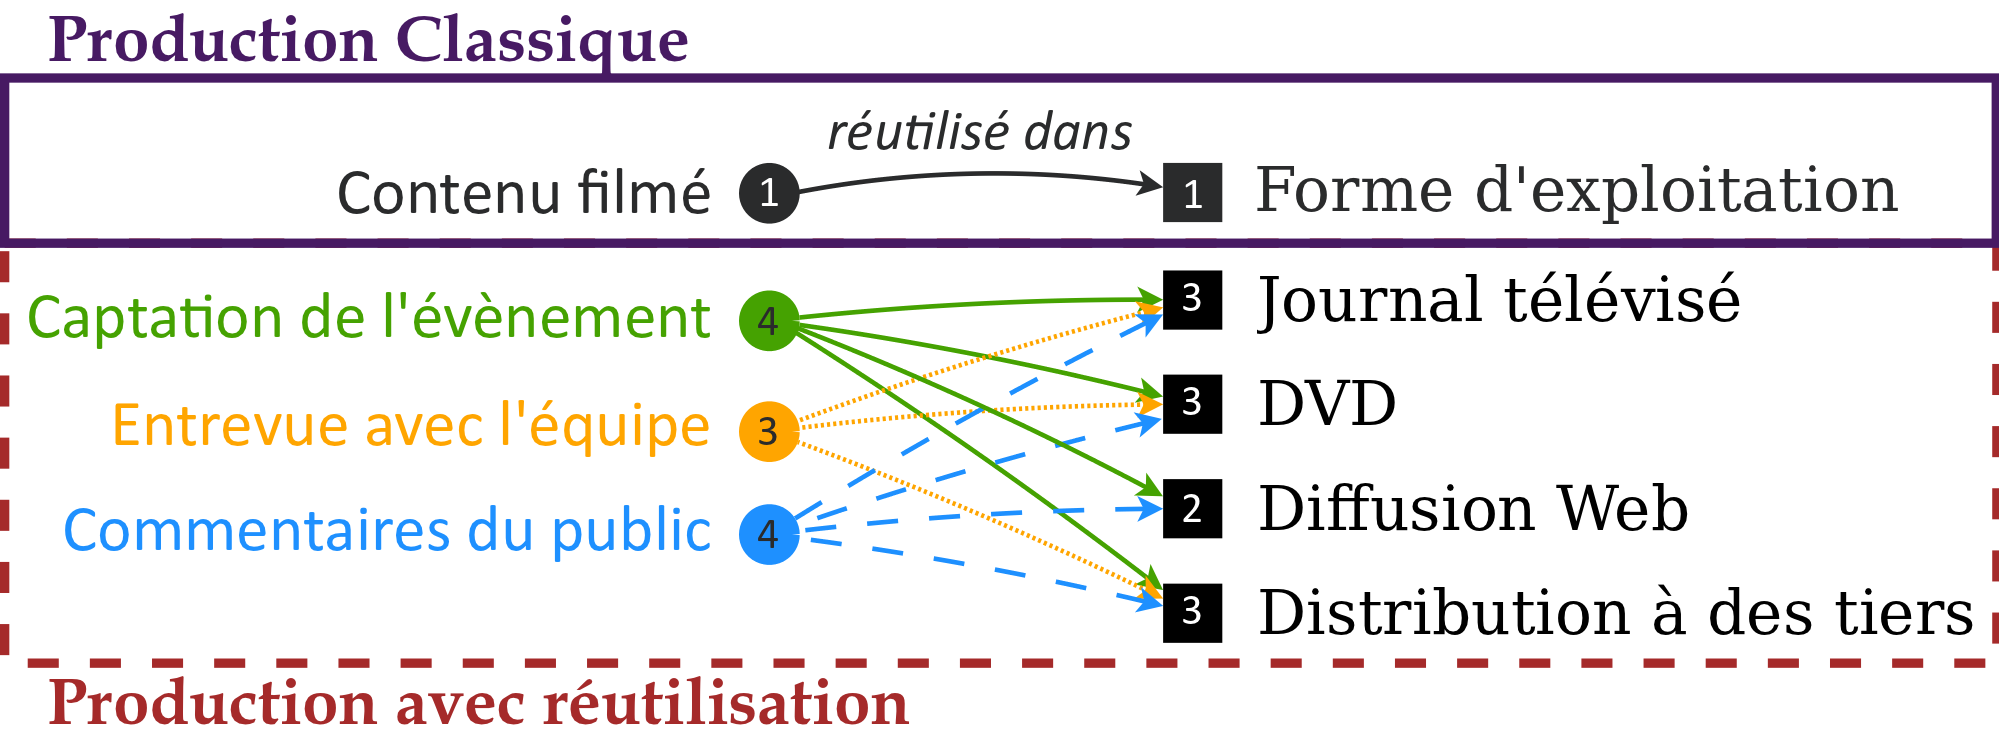
\includegraphics[width=0.7\textwidth]{images/UC-Tahnhauser-v1fr.png}
\caption{Modèle de la production classique comparé avec une production avec réutilisation}
\label{img:intro:reuse}
\end{figure}

Chaque cas de réutilisation tire sa matière première d'à peu près la même base de contenu filmé, mais en tire partie d'une manière propre à chaque forme d'exploitation visée. 
En effet, chaque audience a ses attentes, de même qu'il existe des contraintes techniques spécifiques pour chaque contexte d'exploitation. 
%En effet, il existe des contraintes techniques et des attentes spécifiques à chaque contexte d'exploitation. 

Ces spécificités exigent des variations dans la qualité de l'encodage, le format d'encapsulation utilisé, le montage réalisé, l'habillage du contenu etc. 
Par exemple, les contraintes de diffusion sur le Web implique d'encoder la vidéo dans un format spécifique et de multiples résolutions, généralement plus petites que pour la diffusion télévisée. 
Ensuite, le montage d'une bande-annonce possède un rythme généralement plus rapide que celui des bonus de DVD. 
Finalement, les cas d'exploitation gérés par la chaîne de télévision posséderont un habillage spécifique (logo de la chaîne, message d'annonces etc.) que ne partageront pas forcément les versions vendu à des organisations tierces. 

L'exemple des commentaires du public -- voir la Figure \ref{img:intro:reuse-process} -- permet de montrer à quels moments des transformations doivent être effectuées afin de produire les différentes formes d'exploitation :
\begin{liste} 
	\item[$\bullet$] On considère que deux commentaires de spectateur ont été tournés. 
	\item[$\bullet$] Un des commentaires est intégré au montage du journal télévisé, alors que les deux sont utilisés pour créer la bande-annonce. La bande-annonce est elle-même intégrée au montage du DVD. 
	\item[$\bullet$] Au moment de la finition, l'encodage de la bande-annonce est adapté à la qualité DVD et Web. De même, le journal télévisé est encodé à la fois pour une diffusion en définition standard (SD) et haute-définition (HD).
\end{liste}


\begin{figure}[ht!]
\centering
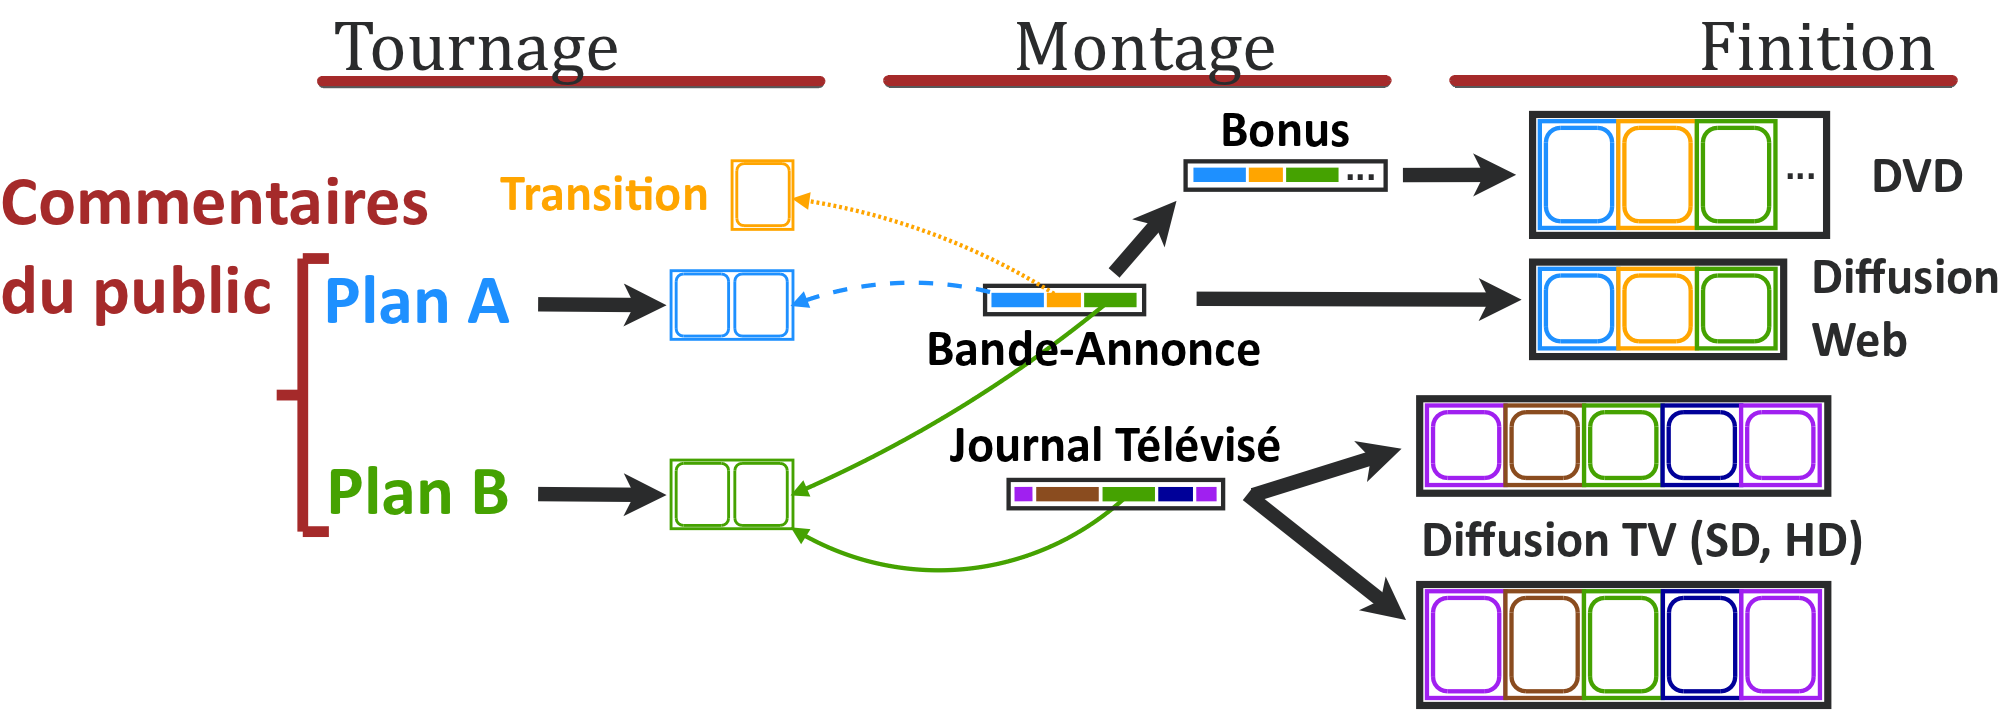
\includegraphics[width=0.8\textwidth]{images/EX-Content-Production-v7fr.png}
\caption{Étapes et transformations des contenus pour chaque forme d'exploitation des commentaires des spectateurs}
\label{img:intro:reuse-process}
\end{figure}

% Dans cet exemple, on distingue deux types d'opérations effectuées sur le contenu ; 
% la sélection de séquences au moment du montage qui correspond à une décision éditoriale (quel contenu va-t-on présenter à l'audience ?) ; 
% la tranformation de l'enregistrement du contenu qui correspond à des choix techniques (quelle méthode d'enregistrement va-t-on utiliser ?).
% Afin de préciser la nature de ces opérations, nous présentons différentes approches de la réutilisation des contenus.


\subsection{Besoins en modélisation (n)}
Le scénario d'usage que nous venons de voir présente un exemple de production incluant directement plusieurs formes d'exploitations pour des contenus produits en collaboration avec deux organisations professionelles et des amateurs. 
Ce scénario permet d'illustrer des opérations de transformation des contenus qui ne se limite pas à une réutilisation brut de matériel. 
On distingue ainsi plusieurs types de transformations qui définissent par les objets d'entrée et de sortie nos besoins de modélisations :
\begin{liste}
	\item le \e{transcodage} d'un contenu d'un format/encodage/résolution à l'autre afin de satisfaire aux contraintes techniques propre à un médium ou un canal de distribution. 
	Par exemple, le journal télévisé distribué dans 2 types de définitions ou bien la bande-annonce préparé pour une diffusion Web et DVD.
	%retraitement

	\item le \e{montage} différencié d'une séquence de contenu suivant la forme éditoriale dans laquelle elle s'insère.
	Le montage des commentaires du public sera plus rapide et dense pour la bande-annonce que pour le journal télévisé. 
	Ce dernier utilisera aussi moins de contenu pour rester sur les commentaires les plus construits ou marquants.
	%rééditorialisation 

	\item l'\e{intégration} d'une séquence montée dans de multiple formes d'exploitations. 
	Par exemple, la bande-annonce est un montage de plusieurs commentaires du public. 
	Elle sert, telle quelle, à la fois sur le site Web de la chaîne et dans les bonus du DVD. 
\end{liste}

De plus, si l'on reprend le scénario depuis la commande de tournage, on se rend compte qu'il existe de nombreux types d'informations que l'on peut collecter sur les objets audiovisuels construits :
\begin{liste}
	\item le genre de l'objet audiovisuel à construire qui détermine un schéma de \e{structure éditoriale}. 
	\item la commande de tournage qui fait office de \e{prescription} de la forme et du contenu de l'objet à produire.
	\item le tournage dont le résultat constitue la \e{réalisation} de la commande, c'est-à-dire le fichier vidéo créé.
	\item une fois le contenu produit, on peut en établir une \e{description} qui se révèlera plus ou moins proche de la prescription.
	\item le montage qui détermine la \e{composition} de l'objet audiovisuel.
	\item l'\e{organisation de la production} de manière générale, c'est-à-dire la division des tâches entre contributeurs. 
\end{liste}

Nos besoins en modélisations peuvent donc se résumer par les assertions suivantes : 
\begin{liste}
	\item[(B1)] rendre les objets et les fragments audiovisuels \g{autonomes} implique de les modéliser sur différents niveaux (technique, esthétique, éditorial etc.). 
	Chaque niveau de modélisation de ces objets correspond au résultat d'opérations effectuées durant le processus de production audiovisuel.
	Ainsi, chaque niveau peut être repris séparément de l'ensemble.

	\item[(B2)] rendre les objets et les fragments audiovisuels \g{réutilisables} implique de leur associer de multiples connaissances dès le début et tout au long de leur cycle de vie.
	Ces connaissances doivent correspondre à celles mobilisées par les contributeurs (humain ou logiciel) de la chaîne de production.
	Chaque type de connaissance s'associe à un niveau spécifique de l'objet audiovisuel de manière à faciliter leur recherche.

	% \item[(B3)] : 
\end{liste}

% À chaque niveau de modélisation des objets et fragments audiovisuels correspond des types de connaissances. 
On notera que la modélisation des objets et des connaissances associées s'enrichit suivant le déroulement de la chaîne de production.
\section{Qu'est-ce qu'un objet audiovisuel numérique ?}\label{sec:dav}
\e{
Dans le monde de l'audiovisuel, certaines notions implicites déterminent la manière dont les professionnels se représentent les objets qu'ils produisent, manipulent, échangent etc. 
L'objectif de cette section est d'expliciter les définitions de ces objets, d'en faire un inventaire (\ref{sec:pv-av}).
Notre démarche ne se limite cependant pas à la vision des professionnels de la production, puisque nous comparons leurs concepts avec ceux d'autres communautés, en vue d'identifier des écarts ou des manques que nous pourrons intégrer dans notre travail.
Ainsi, la communauté des bibliothèques numériques examine plus en détails les relations qui existent entre les résultats d'un processus de création (\ref{sec:pv-bn}). 
La communauté de l'ingénierie documentaire et des sciences de l'information et de la communication invoque quant-à-eux la notion de document, généralement fort absente dans la communauté audiovisuelle, et propose une vision plus fine des différents états de la fabrication et de la consultation d'un contenu audiovisuel (\ref{sec:pv-id}).
Ces deux perspectives apportent une richesse conceptuelle qui, au moment d'examiner les modélisations de l'audiovisuel existantes, nous permettra de mieux identifier ce qu'ils représentent et ne représentent pas.}



\subsection{Du point de vue de l'audiovisuel}\label{sec:pv-av}
Afin de clarifier la notion d'objet audiovisuel, nous présentons la manière dont les professionnels se représentent ses différents composants.
Nous reprenons une liste de définitions proposées par \cite[p.77]{Cox2006} (sauf pour la notion d'\pc{Asset} que nous empruntons à \cite{Austerberry2004}) que nous \ciel{traduisons} et commentons en français : 
\begin{liste}
	\item \pc{Work} (Oeuvre) : \ciel{un travail de création artistique produite ou construite par les efforts conjugués d'une personne ou d'un groupe}.
	Cette définition est clairement reprise du modèle FRBR (voir ci-après) et s'intègre d'ailleurs assez mal avec le reste de la modélisation.

	\item \pc{Essence} : \ciel{toute donnée (numérique) ou signal (analogique) nécessaire à la représentation d'une modalité d'expérience perceptive (visuel, olfactive, auditive etc.)}.

	\item \pc{Material} (Matériel) : \ciel{toute Essence ou combinaison d'Essences (image, son etc.)}. 
	Ainsi, on peut parler de matériel audiovisuel, qui est une combinaison d'Essence audio et visuelle.
	En résumé : Essence/Matériel sont ce que l'on transmet au spectateur, l'Essence se limitant à une modalité.

	\item \pc{Metadata} (Métadonnées) : \ciel{les données qui transportent des informations sur le Matériel -- par exemple des informations d'identification, codage des essences, timeline, propriété intellectuelle etc.}
	Matériel et Essence se différencient des Métadonnées par leur vocation : transmettre une expérience perceptive au spectateur ou transmettre des informations sur le Matériel.

	\item \pc{Content} (Contenu) : \ciel{le Matériel et les métadonnées associées}. 
	Il est particulièrement intéressant de noter l'écart entre cette définition ensembliste et le sens commun. 
	Ici, il s'agit de pouvoir désigner un objet à manipuler, ce qui a de la valeur en terme d'échange, mais non de référer à la signification de l'Oeuvre.
	En résumé : Contenu = Matériel + Métadonnées.

	\item \pc{Instance} : \ciel{une occurrence spécifique et unique de Matériel, Métadonnée ou Contenu}.
	Là encore, l'explicitation de la définition renvoit à un éléments appartenant à trois ensembles. 

	\item \pc{Asset} : \ciel{un asset est ce qui a de la valeur. Le contenu ne suffit pas forcément à représenter un asset. Le propriétaire du contenu doit avoir le droit d'utiliser le matériel avant de pouvoir l'appeler un asset.} 
	En résumé : Asset = Contenu + Droits.
\end{liste}

% On peut résumer ces définitions par l'équation suivante : Asset = Contenu(Matériel + Métadonnées) + Rights.
Cette liste de définition semble intégrer plusieurs manières de se représenter le travail de la production audiovisuelle et ses résultats :
\begin{liste} 

	\item[\g{artistique}] : le travail de création artistique qui aboutit au résultat abstrait d'une Oeuvre. 
	C'est cette réalisation abstraite qui est protégée par la propriété intellectuelle et peut faire l'objet d'une cession de droits.
	Pourtant, la relation entre l'Oeuvre et l'Asset n'est pas établie clairement.

	\item[\g{concrète}] : plusieurs définitions font référence aux résultats concrets de la production (les Instances de Matériel, de Métadonnée et donc de Contenu, les Essences).

	\item[\g{commerciale}] : la notion d'Asset aborde le résultat du travail de production sous l'angle de l'exploitation commerciale. 
	Si on prend l'exemple de la diffusion d'un Contenu qui n'appartient pas à la chaîne, cette diffusion ne peut se faire qu'après achat des droits qui établissent en détails les conditions d'exploitation cédées (zone géographique de diffusion, nombre de rediffusion, limite dans le temps etc.).
	
\end{liste}

% Définition de Media Asset etc. de \cite{Furht2008}.


\subsection{Du point de vue des bibliothèques numériques}\label{sec:pv-bn}
Le \e{Functional Requirements for Bibliographic Records : object-oriented} (FRBRoo) est un modèle conceptuel développé par \cite{Aalberg2008}.
Il vise à faciliter l’échange d’information entre les bibliothèques numériques et les musées. 
Il permet de représenter les personnes participant aux différentes étapes de construction d’un objet culturel, depuis l’idée jusqu’à la réalisation matérielle.

La particularité de cette modélisation est de disséquer les objets culturels dans le but de leur conservation.
Ainsi, le modèle cherche à établir quelles sont les liens généalogiques entre les objets conservés, déterminer les inspirations, les adaptations etc. afin de mettre en évidence des relations culturelles.
Ce souci du détail clarifie les relations entre les objets et par conséquence le processus de création. 
Chaque objet culturel possède trois niveaux de modélisation qui sont présentés dans leur ordre chronologique d'apparition dans le processus de création :
\begin{liste}
	\item le niveau des \e{idées} ou des \e{oeuvres} (\pc{Work}) n’ayant pas pris corps dans une matérialité externe à un sujet (par exemple une mélodie ou une histoire qui nous reste dans la tête). 

	\item le niveau des \e{formes d'expression} (\pc{Expression}) où l'on distingue parmi toutes les formes possibles pour exprimer une idée (une nouvelle écrite, ses traductions, une adaptation de nouvelle en scénario, une lecture de cette nouvelle etc.).
	On se situe à un niveau intermédiaire qui définit des formes abstraites de  réalisation.
	Il faut préciser qu'on parle de forme abstraite dans le sens où il n'existe pas de réalisation concrète, ce qui n'empêche pas de les définir précisement et donc de distinguer de multiples variantes d'expressions :

	\ciel{
	the form of expression is an inherent characteristic of the expression, any change in form (e.g., from alpha-numeric notation to spoken word, a poem created in capitals and rendered in lower case) is a new expression. Similarly, changes in the intellectual conventions or instruments that are employed to express a work (e.g., translation from one language to another) result in the creation of a new expression.} (\cite{Aalberg2008})
	
	\item le niveau des \e{réalisations concrètes} comme les porteurs physiques d’information (\pc{Information Carrier}) portant les expressions (livre, partition, cd-rom etc.). 
	À ce niveau, il faut également distinguer entre l’original (\pc{Manifestation Singleton}) et les copies manufacturées (\pc{Item}) issues d’un modèle de publication (\pc{Manifestation Product Type}). % à rapprocher de la notion de Media Profile dans MPEG-7
\end{liste}

\paragraph{Discussion et comparaison}
Dans la perspective audiovisuelle présentée précédemment, la relation entre Oeuvre et Asset est bien plus floue.
À la fin du processus de création, il apparaît évident que l'on a produit un Asset, mais la notion d'Oeuvre, et donc de l'idée qui a amené à la création, échappe aux systèmes de gestions d'objets audiovisuels.
Ces systèmes ne sont pas fait pour gérer la propriété intellectuelle, ou bien rendre compte des adaptations d'une même idée en plusieurs réalisations.

Par ailleurs, on peut identifier des correspondances entre les notions de FRBR et celles du monde de l'audiovisuel :
\begin{liste}
	\item un \pc{Manifestation Singleton} correspond à la réalisation concrète originale du processus de production, ce qui correspond à la notion de \e{master} dans l'audiovisuel.
	
	\item dans le cadre du numérique, la notion de \pc{Manifestation Product Type} existe dans les cas des documents structurés associés à des feuilles de style.
	On peut noter, que cette notion se rapproche de celle de \pc{MediaProfile} définie dans MPEG-7 à la section \ref{sec:mpeg7}.

	\item un \pc{Item} correspond à une \pc{Instance} de \pc{Contenu} ou de \pc{Matériel}.
	\item un \pc{Information Carrier} correspond à un \e{medium} (media en anglais).

	\item une \pc{Expression} correspond à la notion de \e{format} en audiovisuel.
	Cette notion est centrale puisqu'elle détermine la manière dont la production se déroulera, les moyens attribués, s'il s'agit de l'adapation d'une Oeuvre pré-existante, il faut d'abord vérifier si l'on dispose des droits etc.
	Cette notion est représentée comme une propriété d'un \pc{Contenu} dans ses Métadonnées mais ne permet pas de rendre compte de la relation entre Oeuvre et format d'expression.
\end{liste}





\subsection{Du point de vue de l'ingénierie documentaire}\label{sec:pv-id}
Nous examinons principalement la lignée des travaux de recherche menés initiallement par \cite{Bachimont1998}, formalisés comme une théorie du support numérique dans \cite{bachimont:hdr} puis affinés dans \cite{bachimont:icc}. 
% De nombreux travaux ont repris ce positionnement pour 
Ce positionnement a été approfondi dans le domaine de l'audiovisuel par d'autres auteurs dont \cite{Prie1999}, \cite{Troncy2004}, \cite{Morizet-mahoudeaux2005a}, \cite{Gaillard2008}.

\subsubsection{Les dimensions de l'inscription matérielle}
Ces travaux reposent sur les concepts d'\pc{Inscription}, de \pc{Conte\-nu} et de \pc{Support}. 
La définition d'un \pc{Contenu} permet de relier ces concepts : 
\ciel{
	Un contenu est une forme inscrite sur un support se prêtant à une interprétation à travers laquelle elle fait sens pour quelqu'un ou une communauté.
	C'est donc une \e{forme matérielle interprétable.}} \parcite{bachimont:icc}

Un point à noter est que le contenu est bien une inscription matérielle, non pas le sens que l'on aurait construit de son interprétation.
En tant qu'inscription matérielle, \citeauthor{bachimont:icc} distingue trois dimensions qui caractérisent la manière dont un contenu exprimé sera enregistré, puis restitué.
Dans chacune de ces dimensions (expression, conservation, restitution) intervient une forme, un support et un dispositif, voir la Figure \ref{img:inscriptions}.
Le dispositif a pour objectif de transformer une forme A inscrite sur un support $\alpha$ en une forme B inscrite sur un support $\beta$.

\begin{figure}[ht!]
\centering
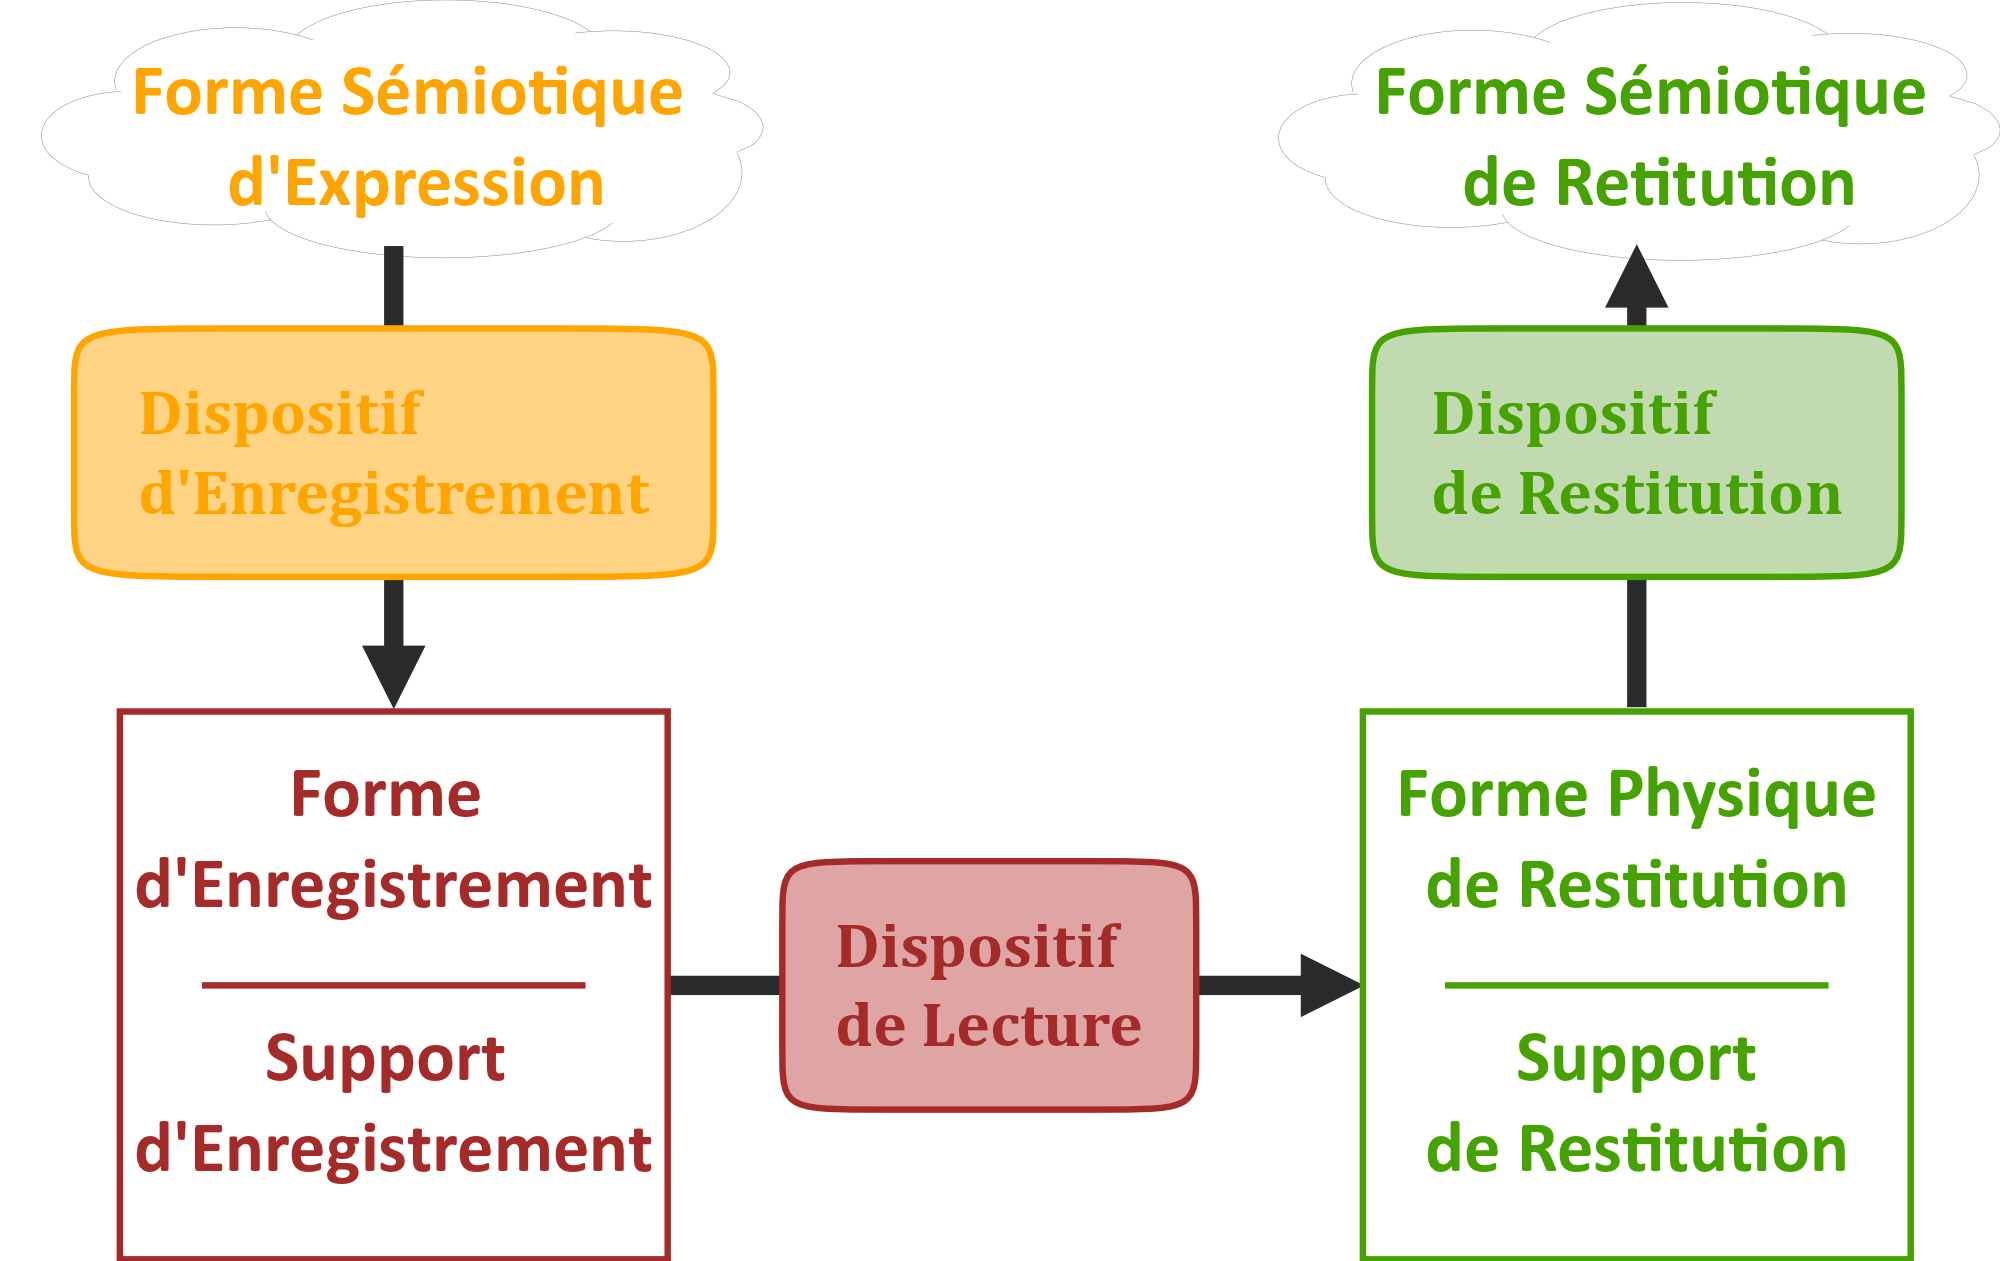
\includegraphics[width=0.7\textwidth]{images/DimensionsInscriptions-v2.png}
\caption{Les dimensions de l'inscription matérielle : forme, support et dispositif}
\label{img:inscriptions}
\end{figure}


\begin{listeni}
	\item \g{dimension de l'expression}
	\begin{liste}
		\item \e{forme sémiotique d'expression} (FSE) : Il ne s'agit pas simplement d'une forme à inscrire, mais bien d'un contenu, puisque l'auteur exprime une intention selon un code sémiotique qui permet à d'autres de l'interpréter.
		La forme sémiotique d'expression est considéré comme volatile et non-permanente, comme la parole ou bien une mélodie sifflée.

		\item \e{dispositif d'enregistrement} (DE) : le dispositif matériel qui réalise l'inscription de la forme d'expression sur un support afin d'assurer sa conservation.
		Cette inscription consiste en une sélection et une configuration de la forme d'expression en une forme d'enregistrement, comme le réalise par exemple un microphone ou bien une caméra.
	\end{liste}

	\item \g{dimension de la conservation}
	\begin{liste}
		\item \e{forme d'enregistrement} (FE) : une forme d'inscription qui assure l'enregistrement, c'est-à-dire la persistance matérielle du contenu sur un support. 
		Par exemple, le code binaire pour un support numérique, un signal mesuré sur une échelle physique quelconque pour l'analogique (magnétique, tension électrique etc.), les lettres de l'alphabet pour l'écriture etc.

		\item \e{support d'enregistrement} (SE) : l'objet matériel sur lequel on inscrit une forme pour conserver et préserver le contenu.
		Par exemple, le papier pour un texte, un 45 tours pour la musique, une mémoire magnétique (disque dur etc.) ou optique (CD etc.) pour le numérique, une cassette vidéo pour une vidéo analogique etc.

		\item \e{dispositif de lecture} (DL) : le dispositif matériel qui réalise la transformation de la forme d'enregistrement en une forme physique de restitution.
		Par exemple, un tourne-disque pour les 45 tours, un ordinateur avec un lecteur multimédia pour une vidéo numérique, un magnétoscope pour une cassette vidéo etc.
	\end{liste}

	\item \g{dimension de la restitution}
	\begin{liste}
		\item \e{forme physique de restitution} (FPR) : une forme sous laquelle l'inscription est présentée pour être perceptible.
		Par exemple, des pixels de couleurs pour une vidéo, une onde sonore pour une musique etc.
		Les normes MPEG-1 et MPEG-2 définissent des techniques d'encodageet de compression d'images et de vidéos.
		Il s'agit donc de normes qui permettent la numérisation de la FPR.
		
		\item \e{support de restitution} (SR) : il s'agit de l'objet matériel sur lequel la restitution du contenu s'inscrit, ce qui permet à un lecteur d'appréhender un contenu par ses sens. 
		Par exemple, un écran pour un signal visuel ou bien l'air ambiant pour le son.
		Cet élément est relié au dispositif de lecture, qui se contente de fournir une forme sans la rendre perceptible à son lecteur, ainsi qu'au dispositif de restitution, qui lui permet au lecteur de l'interpréter.
		
		\item \e{dispositif de restitution} (DR) : le dispositif matériel qui permet de transformer une forme physique en une forme sémiotique.
		Il peut s'agir d'un téléviseur ou d'un écran d'ordinateur pour une forme visuelle, de haut-parleurs pour une forme sonore.
		
		\item \e{forme sémiotique de restitution} (FSR) : une forme de représentation intelligible par l'utilisateur qui en connaît les codes sémiotiques.
		Les formes sémiotiques usuelles sont l'image, la musique, le bruit, la parole etc.
	\end{liste}
\end{listeni}

L'intérêt de cette définition du contenu par état (forme/support) est également de pouvoir introduire la notion de document et de formes documentaires, complètement absente des deux premières perspectives que nous avons examinées.


\subsubsection{Le document audiovisuel numérique}\label{sec:docnum}
\cite{Morizet-mahoudeaux2005a} définissent un document comme un contenu qui peut servir de référence par sa consistance matérielle dans le temps : \ciel{a document is a \e{content} instituted by a \e{publication act}, written down a medium, which possesses a \e{spatial} and \e{temporal delimitation}}.

\begin{liste}
	\item \e{permanence dans le temps} : \ciel{la consistance des signes matériels qu’il porte doit être assurée quelque soit le moment de leur consultation.} \parcite{Bottini2010}

	\item \e{délimitation spatiale} : un document se définit par ce qu'il contient et ce qu'il ne contient pas.
	C'est par ses frontières que le document ouvre la possibilité de sa lecture et de son interprétation.

	\item \e{délimitation temporelle} : la naissance d'un document est institué par un acte de publication, c'est-à-dire le moment où l'on arrête de faire varier sa forme matérielle, pour le faire rentrer dans une sphère médiatique.

	\item \e{intentionnalité} : le document est porteur d'une signification qui ne se résume pas à sa forme matérielle.
	On peut distinguer les documents possédant une intentionnalité \e{a priori} (l'objet matériel a été créé pour porter une intentionnalité documentaire) et ceux dont on attribue une intentionnalité \e{a posteriori} (par exemple, des outils de chasse retrouvés par un archéologue qui les interprètent pour reconstruire les habitudes de l'époque).
\end{liste}


Pour \cite{Leleu-Merviel2004}, le document comporte à la fois une dimension \e{sémiotique} qui renvoit au contenu (signes et sens), \e{technique} qui renvoit aux données (format d'enregistrement, codage et transmission de signaux) et \e{médiatique} qui renvoit à des processus de socialisation, de diffusion, de réception et de consultation.
\cite{Leleu-Merviel2005} décrit cette dernière dimension comme étant la dimension d'accès aux données, un accès qui peut être organisé spatialement et temporellement :
\begin{liste}
	\item la \e{scénique} est la manière de transposer des données en une réalité concrète : \ciel{la forme visuelle et sonore de l’inscription spatiale des fragments}. %FPR+SR
	\item la \e{scénation} est la manière de restituer temporellement à l'utilisateur les fragments d'un document : \ciel{la structure organisée d’événements et/ou d’états avec lesquels l’utilisateur est effectivement mis en interaction}. %DR+FSR
\end{liste}

On retrouve dans cette définition, la caractérisation de l'inscription matérielle faite par \cite{bachimont:icc} avec les correspondances suivantes : 
\begin{liste}
	\item les données correspondent aux éléments matériels qui vont de la FE (l'enregistrement en binaire, inaccessible et illisible pour l'humain) jusqu'à la FPR (qui rend perceptible le contenu). 
	\item la dimension sémiotique renvoit à la FSR ainsi qu'à ses structuration, mais aussi à la configuration par le DR de son accès dans ses dimensions spatiale (scénique) et temporelle (scénation).
	% \begin{liste}
	% 	\item la scénique renvoit à l'association FPR + SR qui rend perceptible le contenu.
	% 	\item la scénation renvoit à l'association FSR + DR qui conditionne l'interprétation du contenu.
	% \end{liste}
\end{liste}

Cette définition développe celle proposée antérieurement par le réseau thématique pluridisciplinaire 33 (RTP-DOC, \cite{Pedauque2003}) qui fait référence dans les communautés scientifiques engagées dans les questions documentaires.
Leur définition du document comporte trois dimensions similaires : le document comme \e{forme} (la dimension matérielle dans laquelle s’incarne le contenu et qui permet sa manipulation), le document comme \e{signe} (il est porteur d’un sens intentionnel), et le document comme \e{médium} (sa dimension sociale, d'échange et de communication).

\paragraph{Le document audiovisuel}
Dans le cas de l'audiovisuel, la forme sémiotique qui est inscrite sur le support d'enregistrement est temporelle, non-interactive et multi-modale.
En effet, les images et le son se présentent au lecteur de manière successive, selon un ordre, un rythme et une durée pré-définis.
La forme audiovisuelle se constitue de la superposition de ces flux visuels et sonores \parcite{Prie1999}.
Or un enregistrement se fait nécessairement sur un espace matériel, ce qui implique de se donner un moyen de représenter spatialement le temps, et d'y associer ces images et ces sons.
L'utilisation de code temporel (\e{timecode}) permet de marquer l'écoulement du temps et de réaliser cette synchronisation des flux.
Une fois cette synchronisation faite, les flux peuvent être lu ensemble pour recréer le flux audiovisuel.
Mais il devient également possible de représenter graphiquement ces flux afin de les appréhender de manière synoptique, quoique imprécise, pour faciliter sa manipulation et son analyse\footnote{Nous mentionnons en particulier le logiciel \gui{Ligne de Temps} développé par l'Institut Recherche et Innovation du Centre Pompidou. Voir \url{http://iri-web.centrepompidou.fr/outils/lignes-de-temps/} pour plus de détails sur son fonctionnement.}. 
En effet, on peut représenter une successsion d'images en sélectionnant à intervalle régulier l'un d'entre elles, pour autant on ne peut réduire l'interprétation d'un objet audiovisuel à cela.
La représentation graphique du son par sa fréquence est bien plus problématique, puisqu'elle ne permet pas de distinguer les moments de paroles et de musique, ni les mots prononcés etc.


 % doc adaptatif
 % doc av
 \subsubsection{Personnalisation et adaptation}
La particularité du document numérique par rapport au document papier, est la coupure entre le support d'enregistrement et le support de restitution. 
Ainsi, l'enregistrement des données ne suffit pas à rendre le document lisible, il faut pour cela la médiation des dispositifs de lecture et de restitution, qui par calcul, reconstruisent le document au lecteur.
Cette reconstruction peut alors faire l'objet d'une configuration prenant en compte la situation de lecture (lecteur, contexte de travail, dispositif matériel etc.), pour proposer non pas une vue canonique du document, mais une vue personnalisée ou adaptée à cette situation.
Ces questions sont traités dans les domaines des hypermédia adaptatifs \parcite{Balpe1990}, de la modélisation utilisateur et des documents virtuels personnalisables \parcite{Leleu-Merviel2004}. \cite{Iksal2002} a réalisé une étude approfondie de ces questions et \cite{Garlatti2004} détaillent leur fonctionnement dans le cadre du projet d'un Web sémantique.

Le fait de nommer les documents ainsi construits de \e{virtuel} renvoit également au caractère dynamique de cette construction, qui s'oppose à la matérialité du document traditionnel, à sa \e{permanence}, son statut de \e{référence} destinée à être \e{partagée} par plusieurs lecteurs \cite[pp.185-186]{bachimont:icc}. 
Ainsi, l'adaptation du document construit des vues perceptibles et manipulables dans l'ici et le maintenant de l'interaction entre le lecteur et les dispositifs de lecture qu'on lui fournit.
Les documents deviennent alors des ressources dont un système se saisit pour composer de nouveaux points de vue, rendu plus pertinent par leur adaptation au contexte de lecture :

\ciel{
conserver, retrouver l’information n’est pas suffisant. 
Pour qu’elle puisse être utile, il faut qu’elle puisse être exploitée, c’est-à-dire traitée et rapprochée d’autres de façon à produire de l’information nouvelle. 
Produire du sens n’est, pour l’essentiel, que rapprocher des informations disparates jamais rassemblées auparavant.} \parcite{Balpe1990}


On remarque que deux types de systèmes d'adaptation se distinguent \parcite{DeBra1999} : 
\begin{liste}
	\item les systèmes \g{adaptables} qui fonctionnent à partir d'une requête de l'utilisateur (quelque soit la forme de celle-ci, formulaire, questionnaire etc.) et des informations sur l'utilisateur (connaissances et préférences).
	Dans ce cadre, l'utilisation d'une modèle de l'utilisateur est primordiale pour mener à bien l'adaptation.
	\item les systèmes \g{adaptatifs} qui repose sur l'observation de l'utilisateur pour déduire ses connaissances et préférences. 
	De la sorte, le système déduit les informations sur l'utilisateur, plutôt qu'il ne le consulte (comme dans la première approche).
\end{liste}

Dans le cadre du projet MediaMap, il est prévu qu'un système \e{adaptable} soit développé pour faciliter la prise de vue par des contributeurs amateurs.
Notre modèle doit ainsi permettre l'adaptation de scripts de tournage, ce qui implique de représenter d'une part les contributeurs et leurs connaissances, le vocabulaire du script et la structure du document audiovisuel.
Toutefois, la manière de réaliser l'adaptation n'est pas traitée dans notre modèle, mais laissée aux développeurs d'applications.
L'objectif de notre modélisation étant de fournir des éléments de contexte pour faciliter les échanges de connaissances le long de la chaîne de production.

% \ciel{
% Cependant en numérique, les fragments existaient, au moins potentiellement, dans la mémoire de la machine, ce n’est que leur actualisation sur l’écran et la forme qu’elle prend qui se construit dans l’ici et maintenant de l’interaction. 
% Celle-ci est donc nécessairement volatile. De plus, elle change à chaque fois.
% Ainsi c’est l’affichage, [\dots] qui varie, mais non le document lui-même tel qu’il est mémorisé au niveau des données.}

% \ciel{
% conserver, retrouver l’information n’est pas suffisant. 
% Pour qu’elle puisse être utile, il faut qu’elle puisse être exploitée, c’est-à-dire traitée et rapprochée d’autres de façon à produire de l’information nouvelle. 
% Produire du sens n’est, pour l’essentiel, que rapprocher des informations disparates jamais rassemblées auparavant.} (\cite{Balpe1990})

% % Deux pistes proposées par SLM : 
% Il est alors possible de construire des assemblage cohérent de fragments le temps d'une consultation (d'un affichage) par un utilisateur (documents virtuels personnalisables).
% Plus on a de connaissance sur son activité, ses tâches, ses compétences propres, plus il est alors possible de rendre cette assemblage pertinent. 

% Il est aussi possible de mettre à profit la description des documents pour construire des notions de voisinage indépendamment du profilage des utilisateurs. 
% La proximité entre deux documents pourra s'évaluer d'autant de manière qu'il y a de critères descriptifs.
% Ainsi, des informations auparavant éparpillées dans des documents papier différents pourraient être regroupés pour former de nouveaux assemblages

\subsubsection{Unité de contenu et structures documentaires}\label{sec:uc-sd}
La distinction entre \e{forme physique de restitution} (FPR) et \e{forme sémiotique de restitution} (FSR) sera essentielle pour l'examen des modélisations de l'audiovisuel.
Un changement de la FSR impacte la signification du contenu, alors que les changements sur la FPR ont une conséquence sur le plan perceptif, mais pas forcément sur la signification (un pixel mort ne change pas le sens d'une image).
Comme nous le verrons plus tard (\ref{sec:codesc}), beaucoup de modèles se focalisent sur la FPR, c'est-à-dire sur la caractérisation du signal par des descripteurs de bas-niveau que l'on pourrait qualifier d'objectif (texture, couleur, forme etc.).

La modélisation de la FSR se fonde sur une interprétation de la forme matérielle du contenu pour dégager ce que \cite{Prie2000} appelle des \e{structures documentaires}.
Une structure documentaire découpe le contenu en unités suivant une grammaire de (dé)composition.
\citeauthor{Prie2000} considère ainsi que \ciel{toute structure est sémantique et fait partie d'une structure d’indexation conceptuelle} qui renvoit donc à une utilisation \ciel{dans le cadre d'une tâche qui peut être une tâche de présentation}.
L'indexation conceptuelle est définie commme \ciel{explicitation de structures et de concepts contenus dans les documents numériques ou qui leur sont associés, pour mieux les exploiter}.
On construira donc des structures différentes suivant l'exploitation du contenu visée, qu'il s'agisse de produire une interprétation pour faciliter l'accès au contenu, de manipuler le contenu ou bien d'en fournir une présentation. 

\citeauthor{Prie2000} distingue ainsi le cas particulier de l'écriture.
Il s'agit d'une tâche à part où \ciel{l’intentionnalité de l’auteur se retrouve plus ou moins dans les structures documentaires} qu'il définit. 
Ces structures expriment des \ciel{connaissances \e{auctoriales} premières}, dans le sens où elles constituent le document et permettent sa médiatisation auprès d'un lectorat.
Cette structure documentaire première renvoit également à un genre documentaire, où elle puise une \ciel{une structure de présentation \e{canonique}}, souvent appelée structure logique par d'autres auteurs.
La notion de genre, amène à la notion de tradition de lecture, dont les éléments de structure canoniques prescrivent une interprétation du document.
Les auteurs peuvent ainsi identifier des communautés de lecteurs par les genres documentaires qu'elles mobilisent dans leurs activités.

La structure première ou canonique définit par l'auteur sert ensuite à d'autres communautés pour établir leur propre structure documentaires en fonction de leurs usages.
Lorsque plusieurs structures sont associées à un document, \cite{Abascal2003} et \cite{Abascal2004} parlent alors de documents \ciel{multistructurés}, chacune répondant aux contraintes d'un usage.

La multiplicité des structures documentaires n'éclaire pas pour autant sur leur nature.
\cite[p.191-192]{bachimont:icc} propose ainsi de distinguer entre quatre niveaux :
\begin{liste}
 	\item \e{niveau physique} : le document est avant tout un assemblage de formes matérielles (unités de contenu), organisées et destinées à faire sens pour un lecteur.

 	\item \e{niveau de typage du contenu} : chaque unité de contenu possède un type qui détermine sa sémantique et les manipulations qu'il peut subir.
 
 	\item \e{niveau syntaxique} : des règles syntaxiques (grammaire) tirent parti du typage des unités de contenu pour régir leur organisation au niveau physique. 

 	\item \e{niveau conceptuel} : le typage d'une unité de contenu lui associe également une signification conceptuelle, indépendante des règles syntaxiques (comme \citeauthor{Prie2000} le fait remarquer avec les structures documentaires).
\end{liste}


La caractérisation de ces différents niveaux nous renvoit aux besoins de modélisations exprimés en \ref{sec:bm-av} (\g{B1 : autonomie} et \g{B2 : réutilisabilité}).

% on propose une modélisation logique du document qui repose sur la vision des contributeurs à sa production.


% paragraph{Discussion et comparaison}

 . 


\newpage
\section{Circulation et réutilisation des objets audiovisuels}\label{sec:gest}

% [Voir MXF, voir AAF ? \cite{Cox2006}
% [Identifiant : hors du cadre de la thèse, dépendant des choix applicatifs des organisations qui utilisent notre modèle. Plusieurs solutions peuvent être implementés via OWL, les URI pouvant être transformé.]

\e{
Si la promesse du numérique de faciliter la manipulation et la circulation des fichiers semble bien s'être réalisée, il n'est pas si évident de l'articuler avec les besoins de la production audiovisuelle (\ref{sec:besoins}).
Ce que l'on nomme la réutilisation des objets audiovisuels recouvre en réalité diverses pratiques et qui repose plus sur la notion d'objet métier ou d'objet numérique que sur la notion informatique de fichier.
Ainsi, la production souhaite récupérer des contenus existants ou produits par d'autres pour les intégrer dans sa propre chaîne de production, ou bien de réutiliser des contenus dans de nouveaux cadres d'exploitations (variation des modes de consommation, de distribution, de public etc.) quelque soit la manière dont l'informatique représente ces objets.}

\e{
Ces opérations qui semblaient a priori plus simple dans un environnement numérique sont en fait plus compliquées qu'il n'y paraît. 
Le numérique impose le calcul et l'explicitation des informations.
Or toutes les informations construites durant la chaîne de production ne sont pas encore intégrées dans les systèmes informatiques actuels.
Lorsque ces informations s'échangent sur papier, à l'oral, par mail ou dans des fichiers non-structurés, le lien avec les objets audiovisuels est alors bien souvent rompu, ce qui entraîne une limitation des traitements réalisables sur ces objets.}

\e{
Dès lors que l'on s'applique à structurer et associer ces informations aux objets audiovisuels, on ouvre la possibilité de récupérer, manipuler, transformer ces objets de nouvelles manières. 
Ainsi augmentés d'un supplément de contexte, les objets gagnent un supplément de manipulabilité susceptible de satisfaire aux besoins de la production audiovisuelle.
Une des solutions développée et utilisée dans l'industrie de la production audiovisuelle est le format conteneur qui encapsule divers types de données en un seul fichier. 
Ainsi, ces formats permettent d'associer de multiples types de fichiers multimédia avec d'autres types d'informations.}

\e{
Cette section a d'abord un souci de clarification des usages et des solutions adoptées. Nous nous intéresserons d'abord aux pratiques de réutilisations (\ref{sec:reuse}), puis nous expliquerons leurs impacts sur la chaîne de production audiovisuelle (\ref{sec:rechaine}). 
Enfin, nous présenterons des formats conteneurs qui assurent le transport des contenus et des informations associées le long de la chaîne de production (\ref{sec:wrapper}).}





%%%%%%%%%%%%%%%%%%%%%%%%%%%%%%%%%%%%%%%%%%%%%%%
\subsection{Caractériser la réutilisation}\label{sec:reuse}
% \subsubsection{Caractérisations de la réutilisation}\label{sec:caracs-reuse}
Nous avons vu grâce à l'exemple de la section \ref{sec:ex-reuse} à quel moment et dans quel type d'opérations la réutilisation pouvait se concrétiser. 
Nous proposons maintenant d'examiner la manière dont différentes communautés scientifiques  abordent la notion de réutilisation. 
Il s'agit de clarifier les hypothèses et les techniques proposées par chacune de ces communautés, et ainsi identifier les éléments pris en compte dans leur représentation du monde.  % Correction ?

\paragraph{Multimédia et Signal}
Prenons d'abord le cas de la communauté multimédia très orientée analyse et traitement du signal. 
Dans ce cadre, les constats mis en avant sont largement les mêmes que ceux que nous avons présentés précédemment (voir section \ref{sec:motiv}, multiplication et diversification des terminaux de lecture et des réseaux de communication, transformation des usages) :
 
\ciel{ 
Hundreds of device profiles are available for accessing online content and more announced everyday. These devices are connected through a wide variety of networks [\dots] As before, the issue of usage scenarios --activity type, user age and gender, time available, and prior knowledge of the subject matter-- continues to exist.} (\cite{Singh2004}).

Un point diffère cependant, le \gui{problème} de la variabilité des usages est considéré comme de même nature que la variabilité des technologies pour transférer et lire le contenu. 
En effet, l'approche de la réutilisation privilégiée par cette communauté consiste en une transformation automatique du contenu en fonction des paramètres d'un scénario de distribution et de lecture : 

\ciel{
Fundamental to this approach is the need to maintain a single copy of the content in its original form and to repurpose the content to fit the desired scenario in real time and in an automated fashion. [\dots] the next step in the repurposing process is to describe the content so that it can be understood and processed to fit delivery requirements --whether they're technical or usage based.} (\cite{Singh2004}).

L'approche automatique est justifiée par la difficulté à maintenir et gérer différentes versions d'un même contenu, en plus d'être coûteux et chronophage.
Ainsi, la décision humaine est simplement reportée au niveau du paramétrage du système de supervisation des opérations techniques.\\


\paragraph{Ingénierie Documentaire}
Dans la communauté de l'ingénierie documentaire, le principe est de pouvoir modéliser distinctement le message que l'auteur souhaite transmettre et la forme dans laquelle ce message se donne à voir par un lecteur. 
Cette tradition, que l'on pourrait faire remonter à la fin des années 60 avec la création du \e{Generalized Markup Language} (\cite{Goldfarb}) ancêtre des SGML, HTML, XML et consorts, repose sur le balisage d'un contenu source. 
Il s'agit alors d'identifier des fragments de contenu ainsi que leur structuration pour mieux les manipuler, quelque soit les opérations effectuées sur ces fragments (transformation, indexation, réécriture etc. \cite[chap.5.2]{Bachimont2004}). 
Les langages de modélisation documentaires tels que \e{Document Type Definition} ou \e{XML Schema} (\cite{Fallside2004}) permettent de contrôler par une grammaire les systèmes de balises construits en vue de formaliser des usages documentaires. 

Nous noterons le développement récent des \gui{chaînes éditoriales}, ces systèmes qui opérationnalisent l'hypothèse de base de l'ingénierie documentaire reformulée par \cite{Crozat2004} de la sorte : \ciel{tout contenu numérique consiste en une ressource qu’un calcul permet de publier dynamiquement sous différentes formes contextualisées}. 

Ces systèmes se concentrent ainsi sur le maintien d'une ressource de base que l'on peut transformer ensuite de diverses manières, soit par une transformation technique que l'on pourra automatisée, soit par une transformation manuelle réglée sur les usages visés (\cite{Crozat2011}) : 
\begin{liste}
	\item le polymorphisme \ciel{consiste en la possibilité technique de disposer d'une source unique de contenu et de la transformer à volonté selon les supports et mises en formes désirés}. Dans ce cas, on établit une séparation entre le fond (la source documentaire) et les formes de publication qui permet de mettre en place une production multi-support.

	\item la réutilisation \ciel{par référence (sans duplication d'information) consiste en la possibilité technique de désassembler et de ré-assembler des fragments de contenu afin de les partager entre plusieurs documents}. Dans ce cas, l'opération repose sur une modélisation séparée du scénario (la structuration) et le contenu.

	\item la ré-éditorialisation est une \ciel{remise en contexte de fragments issus d'un fonds documentaire, par leur ré-agencement au sein d'un nouveau document, leur augmentation par une création de contenus spécifiques et leur publication sur un nouveau support et/ou pour un nouveau public}.

	% \item[T] l'\e{intégration multimédia} est l'exploitation de la propriété héritée du numérique et du codage binaire de permettre l'inscription sur le même support de formes sémiotiques différentes (texte, image, audio, vidéo, ...), afin de composer des contenus multimédia.
\end{liste}

Notons que les chaînes éditoriales s'orientent vers des pratiques de ré-éditorialisation qui sont réalisées manuellement plutôt que de manière automatique.
Les définitions données du polymorphisme et de la réutilisation sont des définitions d'opérations techniques plutôt que des pratiques en tant que telle. 
Ces opérations sont donc permises et prises en charges par les chaînes éditoriales mais ne constituent par leur horizon d'usage.
 % et paramétrées par des règles définies par un utilisateur.
Il semble donc que l'Ingénierie documentaire traditionnelle et le courant lié aux chaînes éditoriales s'intéressent tous deux à des opérations techniques similaires (le polymorphisme et la réutilisation) mais visent des usages distincts qui ne posent pas les mêmes problèmes :
\begin{liste}
	\item D'un côté, il s'agit d'instrumenter d'automatiser des réécritures, entre objets multimédia mais aussi entre documents structurés en XML, base de données etc. 
	Un exemple classique est la création de compte-rendu (ou reporting) qui s'effectue en extrayant des données de diverses sources puis en les intégrant dans de nouveaux documents.

	\item De l'autre on vise à fournir un nouvel environnement de travail aux métiers de l'édition (auteur, éditeur, graphiste etc.) qui permet de passer d'une production artisanale à une production multi-support, réutilisable, ré-éditorialisable. 
	Dans ce cadre, on s'intéresse plus à la création de documents non automatisable telle que les supports pédagogiques par exemple (\cite{Crozat2007}).\\
\end{liste}


\paragraph{Sémiotique Audiovisuelle}
% transition définition Stockinger
Alors que les approches précédentes se concentrent sur des techniques et des outils particuliers, l'approche sémiotique que nous présentons ici propose un point de vue plus général pour définir les différents types de réutilisations existants. 

La sémiotique s'intéresse aux signes pour étudier les activités humaines associées, qu'il s'agisse des producteurs (et de leur intention de communication), des lecteurs (et de leur interprétation des signes produits) ou des relations entre producteur et lecteur (c'est-à-dire des conventions qu'ils partagent). 
Selon \cite{Peirce1978} le \gui{signe} est composé de trois éléments ; le \e{représentamen}, ce qui représente et qu'on pourrait rapprocher de la notion de signifiant chez \cite{DeSaussure1995} ; l'\e{objet}, ce qui est représenté ; l'\e{interprétant} qui produit la relation entre les deux premiers éléments. 

En sémiotique, le signe fait donc toujours l'objet d'une interprétation de la part d'un lecteur qui mobilise un ensemble de conventions pour tenter d'extraire un sens --qui n'est pas forcément l'intention qu'a voulu exprimé l'auteur.
La transmission d'un contenu ne suffit pas en soi à garantir la réussite de la communcation, celle-ci est toujours suceptible d'échouer (soit par un défaut d'expression, un défaut de convention, un défaut d'interprétation). 

Dans ce cadre théorique, la réutilisation de contenu ne se limite pas à une transformation technique (conversion de formats d'encapsulation, de taille d'image, d'encodage) mais se conçoit comme une \gui{adaptation culturelle} \parencite{Stockinger2007} d'une ressource vis-à-vis d'un contexte qui comprend à la fois un usage et une communauté cible. 
Les contenus n'ont donc pas de valeur en soi, mais une valeur d'usage pour une communauté. 
La réutilisation, l'adaptation culturelle ou encore la republication interviennent alors lorsque les contenus sources ne satisfont pas à leur utilisation ou leur communauté de lecteurs future : 

\ciel{
La \e{republication} (en anglais re-authoring ou re-purposing) recouvre un ensemble d'activités visant à réutiliser un corpus de documents numériques (textuels, audiovisuels, visuels, etc.) pour des usages spécifiques auxquels les documents sources, dans leur forme initiale, ne peuvent que partiellement répondre} \parencite{Stockinger2007b}.


On l'aura compris, ce processus englobe des opérations techniques et éditoriales et place les conventions des communautés dans une position centrale. 
Pour ce qui est de caractériser des communautés d'utilisateurs, \pc{Stockinger} se réfère à des sociologues dont \cite{Bourdieu}, et propose différents critères de regroupement :
% la notion d'habitus développée par
\begin{liste}
	\item le temps ou l'espace occupé
	\item les activités et les objectifs recherchés
	\item les attentes et les intérêts
	\item les compétences linguistiques
	\item et de manière générale les connaissances ou les représentations
\end{liste}

Une fois une communauté cible identifiée, il est alors possible ; (1) de définir le type et la forme de contenu qui est pertinent (utilisable, utile, compréhensible, acceptable etc. par ces utilisateurs) ; (2) les outils nécessaires pour effectuer les opérations propres à adapter le contenu aux besoins de la communauté cible :

\ciel{
La republication est donc un processus, parfois très complexe, d'adaptation d'un document ou d'un corpus de documents sources à des usages spécifiques. Ce processus d'adaptation peut concerner tous les plans constitutifs d'un document (Stockinger, 1981, 1999 et 2003), c'est-à-dire aussi bien le plan du contenu que celui de l'expression. Il s'accomplit à travers un ensemble d'activités intellectuelles et de gestes techniques et en référence à des modèles ou genres de publications qui intègrent les contraintes typiques des contextes et des communautés d'usage auxquels un document ou un corpus de documents republiés est destiné} \parencite{Stockinger2007b}.

% opérations : (traitement linguistique, restructuration, rééditorialisation).
La republication repose donc sur une représentation des communautés d'utilisateurs, de leur capacités d'interprétation ainsi que sur une représentation des contenus dont elles disposent habituellement. 
La republication se définit selon \parencite{Stockinger2007} suivant les critères suivants : 
\begin{liste}
	\item \e{les opérations à effectuer} ; sélection, réorganisation, ajout d'explications, ajout d'éléments complémentaires, traduction, mise en lien avec d'autres ressources, modification de la forme d'expression, création de nouveau contenu etc.
	\item \e{le type} (image, texte, objet audiovisuel etc.) \e{et le genre} (journal télévisé, émission etc.) \e{de ressources à traiter}. 
	\item \e{l'objectif de la réutilisation} ; le contexte d'usage, la communauté cible, le genre de la future publication, le format de distribution etc.
	\item \e{les ressources à disposition pour effectuer la republication} ; les personnes, les outils, le budget, les ressources intellectuelles.
\end{liste}
Cette approche générale de la réutilisation n'est pas purement intellectuelle puisqu'elle se concrétise également dans des développements logiciels. 
En effet, un logiciel nommé \gui{Atelier Sémiotique} se développe dans le cadre de l'\gui{Atelier de Sémiotique Audiovisuelle} et par l'intermédiaire de divers projets (Saphir, Logos) et partenaires (INA, ESCoM, MSH de Paris).

\paragraph{Discussion}
% Notons que cette définition, par rapport à celle des approches précédentes, décrit de manière plus globale ce qu'est la réutilisation en citant de nombreux et nouveaux éléments à prendre en compte. 
% L'analyse proposé par la sémiotique audiovisuelle propose une définition plus générale de ce qu'est la réutilisation. 
L'analyse proposée par \pc{Stockinger} propose une définition générale de la réutilisation qui englobe les pratiques présentées précédemment. 
En effet, l'ingénierie documentaire et la communauté multimédia se concentrent sur la construction d'outils pour automatiser certaines transformations ou réécritures de contenu.
En se concentrant sur un éventail de techniques, ces approches se prêtent plus à certains cas d'usages et visent des objectifs différents. %(comme la ré-éditorialisation pour l'ingénierie documentaire ou bien la construction automatique de compte-rendu pour la communauté multimédia).
% parler de C2M qui vise à une chaîne éditoriale multimédia ?  

\begin{figure}[ht!]
\centering
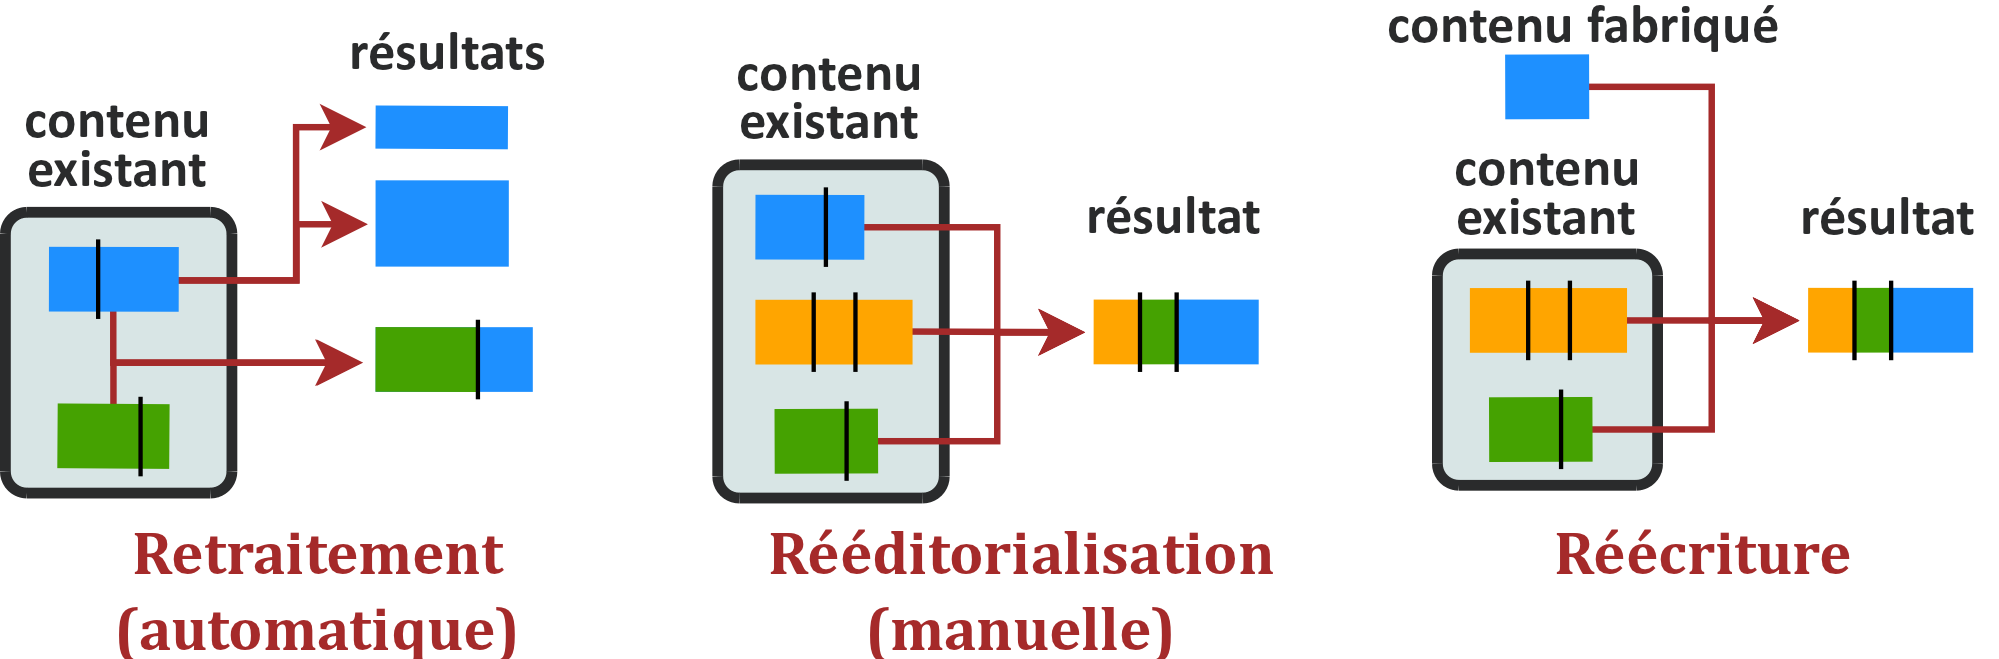
\includegraphics[width=0.75\textwidth]{images/Reuse-v1.png}
\caption{Les différentes pratiques de réutilisations}
\label{img:intro:reuse}
\end{figure}

Nous proposons donc de définir la terminologie suivante pour distinguer entre trois niveaux successifs de réutilisation, chacun visant à créer un nouveau document mais suivant des opérations différentes (voir Figure \ref{img:intro:reuse}). 
La premier critère distinctif est l'automatisation de la transformation, le second critère repose sur la création originale de contenu plutôt que la réorganisation d'un existant : 
\begin{liste}
	\item le \eg{retraitement} (repurposing) qui se caractérise par une automatisation de la transformation opérée sur le contenu (quelque soit son type), c'est-à-dire que cette transformation est effectué par un logiciel lui-même paramétré par un humain. 
	Ces transformations visent à modifier la forme d'expression du document, extraire des fragments de contenu de différentes sources pour les aggréger dans un nouveau document, ou bien encore réorganiser automatiquement la structure du contenu. 
	Le retraitement dépasse le polymorphisme en ce sens où il est possible de gérer de multiple sources de contenus pour construire dynamiquement un nouveau document. 
	Dans le cas de l'audiovisuel, il s'agit des pratiques de réencodage, de changements de format d'encapsulation etc.
	Pour reprendre l'exemple précédent (\ref{sec:ex-reuse}) d'un contenu TV pour une diffusion Web, ou bien encore la création automatique de résumé de rencontres sportives etc. \\

	\item la \eg{rééditorialisation} (reediting) se caractérise par une transformation (manuelle et automatique) de contenus existants. 
	Le document doit s'adapter à un nouveau contexte de lecture (genre éditoriale, public, forme d'expression etc.).
	La transformation du contenu nécessite une compréhension du nouveau contexte de lecture et consiste en des opérations de réorganisation, de mise en relation avec d'autres contenus, de traduction etc. 
	Ces opérations ne se limitent pas à une transformation de la forme d'expression du document (retraitement) mais ne constituent pas une création originale de contenus (réécriture). 
	Simplement, on réutilise divers contenus existants pour créer un nouveau document.  
	La ré-éditorialisation repose donc sur le polymorphisme et la réutilisation au sens de \cite{Crozat2011}.
	Dans le cas de l'audiovisuel, il s'agit typiquement de pratiques de re-montage et de nouvelles sélections de contenu. 
	Pour reprendre l'exemple précédent, il s'agit de monter différemment une séquence initialement prévue pour un journal TV et qui doit s'insérer dans un DVD etc. \\

	 
	\item la \eg{réécriture} (reauthoring) se caractérise par une transformation de contenus existants accompagnée d'une création de contenu original. 
	L'ajout de contenu sert à satisfaire soit aux attentes spécifiques du nouveau public cible, aux contraintes d'un nouveau genre éditorial (commentaires, explications, exemples etc.) soit à la création d'une version augmentée d'un document existant (pas de changement de public cible, mais de nouvelles attentes).
	Dans le cas de l'audiovisuel, il s'agit par exemple de la construction d'un documentaire à partir de vidéo d'archives, la création originale étant le commentaire proposé.\\	 
\end{liste}

Les pratiques de réutilisations sont donc chevillées aux dimensions techniques, éditoriales et sémiotiques du contenu audiovisuel. 
Leur mise en place pose également des problèmes dans l'organisation de la chaîne de production audiovisuelle et son informatisation
% Il faut donc élargir le champ de la modélisation des contenus à une dimension sémiotique et éditoriale et faire le lien avec le déroulement de la production.








%%%%%%%%%%%%%%%%%%%%%%%%%%%%%%%%%%%%%%%%%%%%%%%
\subsection{Évolutions de la chaîne de production}\label{sec:rechaine}
\e{
Les changements introduits par la réutilisation dans la chaîne de production sont donc plus vastes qu'une simple adaptation technique à de nouveaux modes de distribution. %(canal de diffusion + terminal de lecture). 
Il s'agit également de prendre en compte l'audience visée pour affiner encore plus l'adaptation du contenu à ses futurs consomateurs/lecteurs.
L'objectif est de favoriser le développement de variantes d'un même programme soit par la restructuration du contenu (retraitement ou rééditorialisation) ou par l'ajout de contenus (réécriture). 
L'introduction d'acteurs tiers dans une chaîne de production pour fabriquer ou fournir du contenu ne peut se faire sans une plus grande maîtrise des contenus et une meilleure description de ces derniers dès la pré-production.
En effet, le client qui souhaite déléguer la fabrication de contenu à un fournisseur tiers doit d'abord définir ses attentes. 
À l'inverse, si le fournisseur connaît son contenu le client lui a besoin d'un descriptif pour sélectionner les fragments les plus pertinents.
Ainsi, les chaînes de production des clients et des fournisseurs doivent évoluer pour gérer (fournir/acquérir) non pas juste du contenu, mais des descriptions (adjointes ou pas à du contenu) facilitant le travail de leurs partenaires (fabrication ou réutilisation).
}
% Le producteur-diffuseur rentre alors dans une dynamique d'adaptation de ces contenus.

Comme nous l'avons constaté en \ref{sec:electro}, le développement de l'électronique offre de nouvelles opportunités de production mixte, soit avec des amateurs, soit avec d'autres professionnels. 
Cependant, une organisation souhaitant profiter de ces opportunités devra réussir d'abord à encadrer ses partenaires et clarifier avec eux les termes de leurs accords. 
Ce qui auparavant pouvait se résoudre \e{de visu} ou de manière informelle doit maintenant être explicité afin de clarifier la demande, c'est-à-dire le contenu souhaité. 
Qu'il s'agisse de passer commande, ou bien de rechercher dans des bases existantes, cette étape s'apparente à la définition du besoin, à l'écriture d'un cahier des charges, ou dans les termes propres à la production audiovisuelle, au \e{Scripting} défini en \ref{sec:preprod}. 
Maintenant que la fabrication du contenu est déléguée à des tiers, il reste cependant à récupérer le résultat et à vérifier qu'il satisfait à la demande initiale. 
Cette dernière étape nommée généralement \e{Acquisition} constitue un travail à part entière puisqu'il s'agit de \gui{faire rentrer} le contenu dans les \gui{cases} du système d'information et de gestion des contenus. 
En plus des questions de formats informatiques, s'ajoute souvent le problème de la description des contenus et de leur classification en vue de leur utilisation future.  
L'acquisition dépend grandement des conventions établies avec le fabricant/livreur de contenu et impacte directement sur le temps passé à faire le \e{derushing}. 

Côté client, on transforme d'abord la phase de scripting en l'expression d'une \pc{Commande} ou d'une \pc{Requête} ce qui permet de déléguer la fabrication des contenus à un tiers.
Ensuite, on vérifie par \pc{Acquisition} du contenu que le résultat correspond bien à la demande et on procède aux ajustements nécessaires (si besoin) pour satisfaire aux contraintes de notre système (voir Figure \ref{img:intro:evochain}). 

\begin{figure}[ht!]
\centering
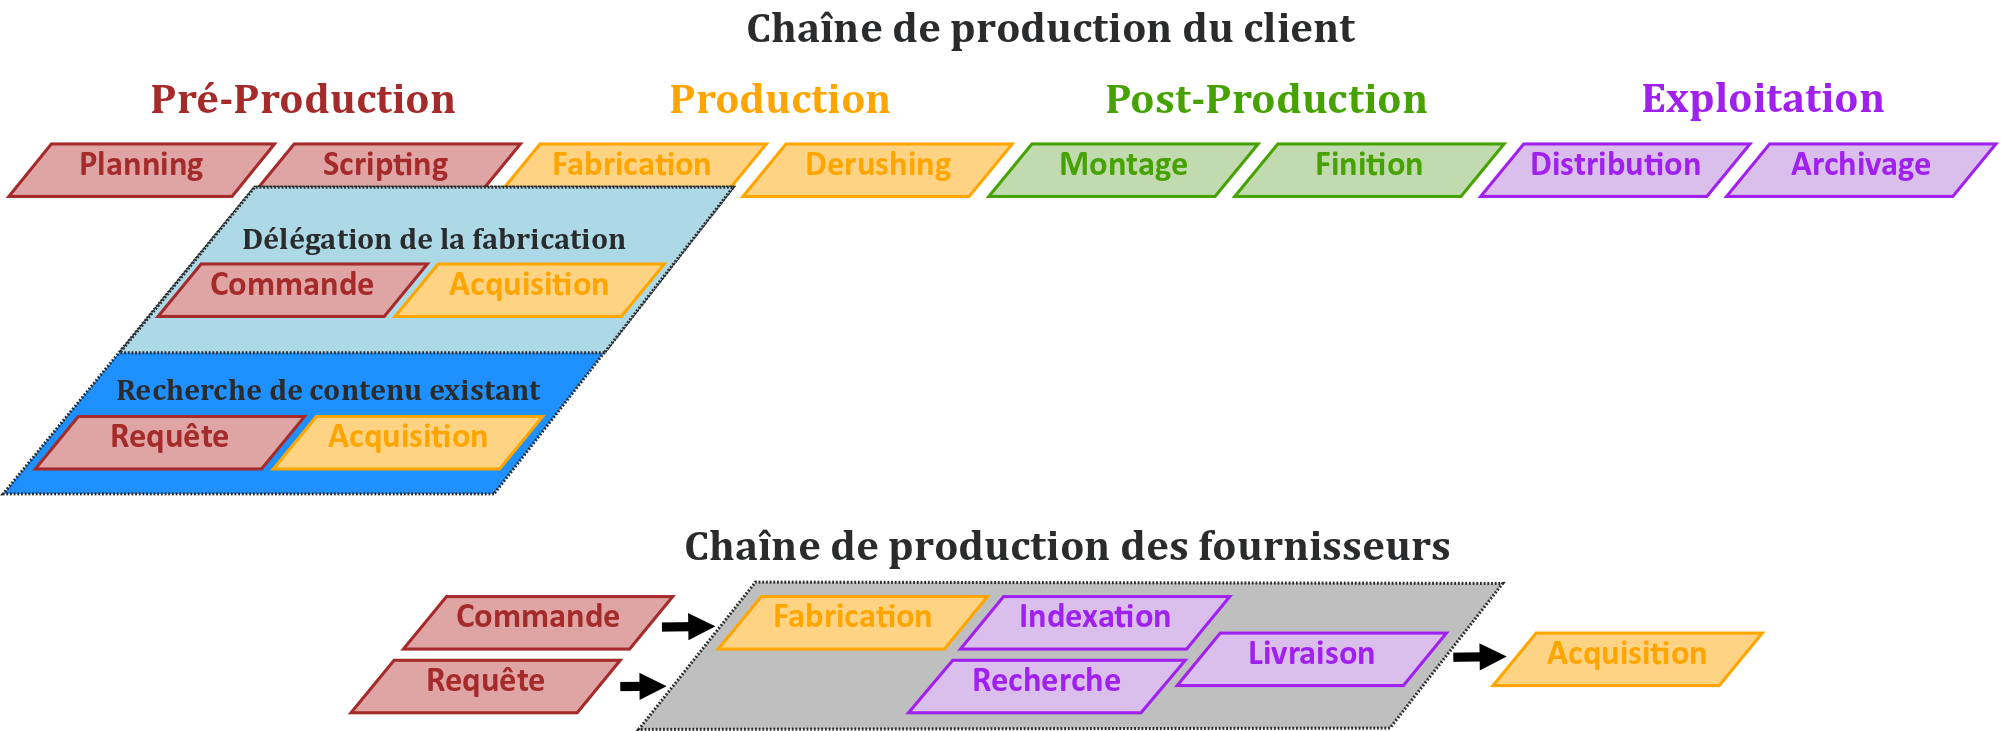
\includegraphics[width=\textwidth]{images/Workflow-Thesis-v6.png}
\caption{Ouverture des chaînes de production du client et du fournisseur}
\label{img:intro:evochain}
\end{figure}

Du côté des fournisseurs de contenu, il existe une distinction entre les chaînes du fabricant et du fournisseur du contenu :  

\begin{liste}
	\item \e{déléguer la fabrication à des contributeurs tiers} : l'utilisation du scripting pour définir la \pc{Commande} de contenu attendu semble une solution satisfaisante, à condition que le vocabulaire utilisé soit normé et rattaché à une conceptualisation de manière à éviter la confusion ou les différences d'interprétations. 
    Lorsqu'il s'agit d'amateurs, la situation se complique car on ne peut pas s'appuyer sur une conceptualisation commune de la production audiovisuelle pour clarifier la commande. 
    De plus, le manque d'expérience et l'ignorance des usages du métier impliquent non seulement de documenter les concepts par des mots et des définitions, mais aussi d'expliquer ce qu'il faut faire durant la phase de \pc{Fabrication}. 
    En d'autres termes, en travaillant avec des amateurs, les professionnels ne se retrouvent non pas à écarter la confusion entre des mots se reférant au même concept, mais à expliquer les opérations auxquelles ces concepts font référence. 
    De même pour l'acquisition, s'il s'agit surtout de se mettre d'accord entre professionnels, travailler avec des amateurs semble plus difficile de prime abord. 
    Les notions de formats d'encodage et d'encapsulation sont souvent confuses ou se mélangent, de même que la description des contenus peut s'avérer compliquée à réaliser sans expérience préalable. 
    Tout du moins, il faut remarquer que la description de la demande initiale sert de description a minima du contenu produit, même si les variations ou les écarts ne sont pas forcément indiqués.
    Le cas échéant, une phase d'\pc{Indexation} peut être nécessaire pour décrire le contenu suivant les exigences du client.\\

	\item \e{rechercher des contenus existants depuis les bases professionnelles} : l'utilisation du vocabulaire de l'écriture audiovisuelle pour définir une \pc{Requête} nécessite une indexation utilisant ce même vocabulaire, ou alors une manière de traduire la requête d'un langage à l'autre (par alignement des vocabulaires par exemple). 
	De même, il faut pouvoir s'accorder sur le niveau de fragmentation recherché (programme complet, séquences, scène, frame etc.), le format du contenu, les descriptions ou les métadonnées à fournir etc.
	Ainsi, la \pc{Livraison} de contenu ne consiste pas en un simple transfert de fichier, mais représente le moment où l'on teste l'interopérabilité entre les systèmes et les formats. 
	Cette étape est d'autant plus cruciale qu'elle se répercute directement sur la phase d'acquisition pour le client. 
	Tout ce qui n'a pas pu être résolu à la livraison (côté fournisseur) devra l'être au moment de l'acquisition dans le système (côté client).\\
	% un vocabulaire de requêtes, s'accorder sur les niveaux de fragmentation, le format de livraison, le contenu de la livraison
\end{liste}



Finalement, il nous faut encore éclairer à quels moments dans la chaîne de production les différentes pratiques de réutilisation sont réalisées (voir définition en \ref{sec:reuse}).
De manière générale, on considère que la réutilisation commence à la phase de pré-production, au moment du \pc{Planning} et du \pc{Scripting} où l'on spécifie les nouvelles formes et formats d'exploitation (voir Figure \ref{img:intro:reutilisation}). 
Mais chaque pratique opére à différents étapes de la chaîne :
\begin{liste}
	\item pour le \e{retraitement}, les variations sur la forme d'expression du document se réalisent en phase de \pc{Finition}. 
	C'est à ce moment que l'original et les variantes sont encodés et encapsulés dans les formats correspondants à leur mode de distribution. 
	Lorsqu'il y a manipulation de la structure des contenus, ces opérations (automatisées) se réalisent à la phase de \pc{Montage}.

	\item pour la \e{rééditorialisation}, le travail commence en phase de \pc{Derushing}, par la sélection des séquences de contenu à ajouter ou à retirer du contenu original. 
	La grande différence avec le retraitement, c'est que cette sélection s'effectue manuellement sur les contenus à disposition. 
	Ensuite, on opére un nouveau \pc{Montage} qui peut également impliquer une \pc{Finition} différente.

	\item pour la \e{réécriture}, la grande différence avec les autres pratiques est que l'on ajoute une nouvelle phase de \pc{Fabrication}. 
	Qu'il s'agisse de création originale ou de récupération de contenu chez un fournisseur tiers, la réécriture consiste à utiliser de nouveaux contenus. 
	Ensuite, on sélectionne en \pc{Derushing} les séquences qui permettront de réaliser un nouveau \pc{Montage}. 
	Finalement, plusieurs \pc{Finition} sont à envisager suivant les cas d'exploitation.
\end{liste}
% conséquences de la réutilisation dans la chaîne : à quel étape ça se joue

\begin{figure}[ht!]
\centering
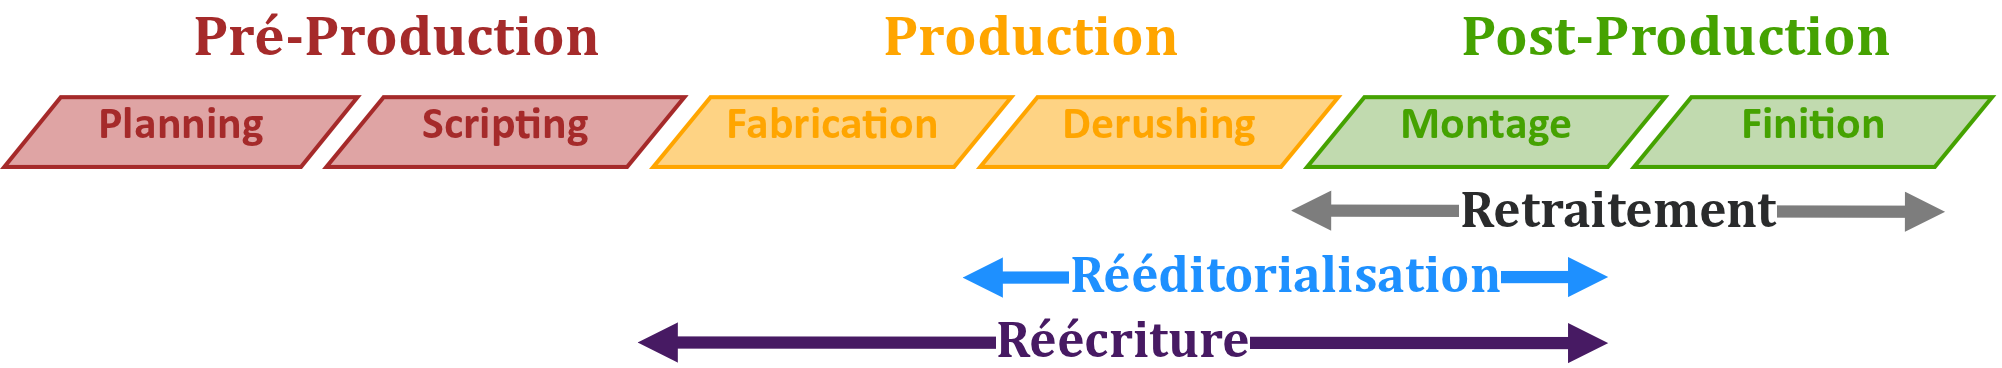
\includegraphics[width=0.8\textwidth]{images/Workflow-Reuse-v1.png}
\caption{Les différentes formes de réutilisation et leur mise en oeuvre dans la chaîne de production audiovisuelle.}
\label{img:intro:reutilisation}
\end{figure}








\subsection{Formats conteneurs pour l'audiovisuel} \label{sec:wrapper}
% intro
Les formats conteneurs sont des formats de fichiers qui encapsulent des contenus de toutes sortes (audio, vidéo, texte, image etc.). 
Un des exemples le plus connu pour la vidéo est le format AVI de Microsoft, souvent confondu avec un format de compression. 
Ces formats ont la particularité d'associer aux contenus audio-visuels des informations annexes, le plus souvent sous la forme de métadonnées.
L'intérêt de ces formats est de constituer un objet numérique qui structure l'enregistrement du contenu et de ses informations annexes et fournit ainsi une manière unique d'y accéder (\cite{Ferreira2010}).
Sans cela, les informations seraient dispersées et le lien avec le contenu devrait se faire via des références. 
Cette force constitue également un inconvénient lorsqu'il n'est pas possible de faire évoluer le modèle d'information ou bien d'en changer en fonction du type de production ou d'exploitation envisagé.

Dans le cas de la production télévisuelle, deux formats liés et complémentaires ont été progressivement adoptés par l'industrie.  
Il s'agit du \pc{Material eXchange Format} (MXF) et de l'\pc{Advanced Authoring Format} (AAF) que nous présentons par la suite. 
Leur particularité est de pouvoir intégrer des schémas de métadonnées propres aux besoins de l'industrie, mais aussi de pouvoir en utiliser d'autres. 
Comme ces formats servent de référence à l'industrie, il est particulièrement intéressant pour nous de comprendre leur modélisation de l'objet audiovisuel, de voir comment ils gèrent les résultats intermédiaires de la chaîne de production ou quels genres d'informations ils embarquent avec le contenu.


\subsubsection{Material eXchange Format}\label{sec:mxf}
% qui / quand
MXF est un format conteneur ouvert développé depuis le milieu des années 90 par des membres de l'industrie et standardisé en 2004 par la \pc{Society of Motion Picture and Television Engineers} (SMPTE).
% objectif
Son objectif est de favoriser les échanges de contenus audio-visuels finis en les associant à d'autres données ou métadonnées (\cite{Devlin2002}).
Ces métadonnées sont structurés par le schéma \pc{Descriptive Metadata Scheme-1} (DMS-1, ) que nous présenterons en détails dans la suite de la section. 

% description
Voici d'abord les principales caractéristiques de MXF en tant que format (\cite{Ferreira2010a}) : 
\begin{liste} 
	\item \e{indépendant d'un système propriétaire}. 
	Le standard se veut avant tout un format qui fonctionne sur tout systèmes. 
	Ainsi, il définit une organisation des données bit par bit qui repose notamment sur le système de \pc{Key-Length-Value} (KLV, clé-longueur-valeur). 
	La clé donne un identificateur de l'élément à suivre, la longueur précise la taille de la valeur à suivre et la valeur contient les données de l'élément.
	Comme dans tout format de fichier, on retrouve la définition d'en-tête et de fin de fichier. 
	L'en-tête contient des métadonnées de description du contenu (\pc{Header Metadata}), de sa structuration (\pc{Partition Metadata}) et une table d'association entre un timecode et une position dans le flux binaire du fichier (\pc{Index Table}).

	\item \e{indépendant des méthodes de compression du contenu utilisées}.
	MXF définit une structure d'encapsulation et d'accès au contenu nommé \pc{Essence Container} (EC) qui permet de transporter du contenu sans le transformer ou bien de faire référence à des fichiers externes.  
	MXF possède des transpositions permettant de synchroniser différents flux de contenus, quelque soit leur encodage. 
	Chaque type de contenu est traité à part, ainsi les EC sont composés de \pc{Content Package}, eux-mêmes décomposé en \pc{Picture Item} (piste vidéo), \pc{SoundItem} (piste audio), \pc{Data Item} (télétexte, sous-titre etc.), \pc{Compound Item} (contenu audiovisuel encodé comme un seul contenu) et \pc{System Item} (autres données comme les timecode etc.).
	La Figure \ref{img:mxf-content} montre deux méthodes d'encapsulation de ces essences.


	\item \e{diffusable en flux continu ou bien par fichier}. 
	Suivant la méthode d'organisation de l'EC décrit ci-dessus, le contenu d'un fichier MXF peut être visionné au cours de son transfert (streaming). 
	Cette caractéristique est particulièrement importante dans le cadre de la diffusion télévisuelle et s'applique à tout les types de contenu d'un MXF (audio-visuel, mais aussi sous-titre ou métadonnées etc.). 
	Naturellement, le fichier MXF peut également être transféré en FTP.

	\item \e{une organisation des contenus indépendante de leur visionnage}. 
	En effet, MXF définit à part l'organisation des contenus encapsulés et la manière de les visionner.
	Le \pc{Header Metadata}	d'un fichier MXF contient une partie \pc{File Pacakage} (FP) qui décrit la manière dont les fichiers de contenus sont encapsulés dans le MXF. 
	Cette description détaille les méthodes d'encodage pour toutes les pistes de contenus (Track) du fichier, de même que les timecode originaux.
	Cependant, si le FP décrit les sources d'un fichier MXF, il existe également un \pc{Material Package} (MP) décrivant la manière dont celles-ci doivent être visionnées.
	Il s'agit là de définir un montage simplifié qui explicite quelle partie et dans quel ordre jouer les contenus sources, à la manière d'une \ciel{Edit Decision List}. 

	\item \e{encapsulation conjointe des contenus et des métadonnées}. 
	Comme nous l'avons vu, un fichier MXF contient un \pc{Header Metadata} transportant des métadonnées propres à l'ensemble du fichier ainsi que des métadonnées propres à chaque paquet de données (Package). 
	Ces éléments sont donc intégrés dans la structure du fichier, au même titre que le contenu.
\end{liste}


\begin{figure}[ht!]
\centering
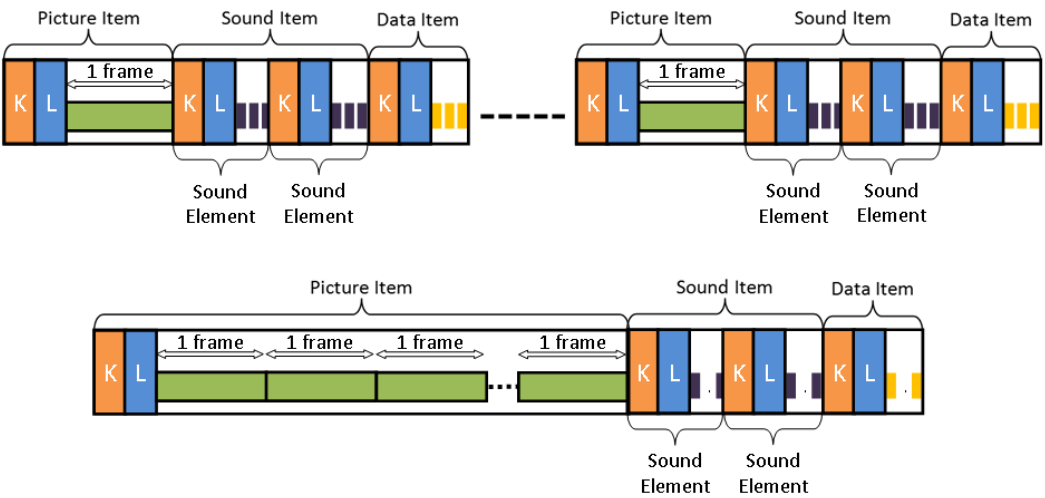
\includegraphics[width=0.9\textwidth]{images/MXF-ContentPackage.png}
\caption{Deux méthodes d'encapsulation des essences en MXF : image par image (haut, pour le streaming), par séquence vidéo (bas).}
\label{img:mxf-content}
\end{figure}

\paragraph{Adoption et usage}
Du fait de sa large adoption par l'industrie de la télévision, il favorise l'interopérabilité entre les systèmes, souvent propriétaires, des producteurs, diffuseurs, chaînes de télévision etc. (\cite{Ferreira2010}, \cite{Devlin2002}). 
Cependant, MXF n'est pas fait pour gérer les résultats intermédiaires de la chaîne de production. 
Il a été spécifiquement conçu pour favoriser la circulation des programmes finis, indépendamment de la manière dont les contenus sont matériellement enregistrés et structurés.
De ce fait, MXF se positionne comme un format utilisé en fin de chaîne de production, à la diffusion des programmes ou bien dans le cas d'échanges entre professionnels.

\subsubsection{Description Metadata Scheme-1}\label{sec:dms-1}
Le schéma DMS-1 a été standardisé par le SMPTE en 2004 (\cite{Smpte2004}).
Il propose trois schémas de description (\pc{Framework}), chacun proposant une perspective de description particulière : 
\begin{liste}
	\item le \pc{Production Framework} propose une description du fichier MXF en tant que résultat d'une production. 
	Les informations qu'il regroupe s'appliquent donc au fichier en entier (identification, propriété intellectuelle, droits et contrats, projet, format de publication, format d'image, récompense) mais aussi au contenu de l'objet audiovisuel (évènements relatés, période historique, annotation).

	\item le \pc{Clip Framework} aborde la description du point de vue de la création du matériel audio-visuel, c'est-à-dire des séquences de contenu encapsulées dans le MXF. 
	On retrouve des informations liées à la production (projet, droits et contrat) mais surtout des éléments pour décrire les essences (format de l'image, sous-titre, script utilisé, matériel utilisé et paramètrage, opérations de transformation des essences) et une description par plan.

	\item le \pc{Scene Framework} propose une vision éditoriale du contenu en le découpant en scène et plan. 
	Ces éléments sont ensuite décrits en terme d'évènements, en précisant les participants et les lieux où ils se déroulent etc.
\end{liste}

\paragraph{Framework et ensemble de métadonnées}
Ces \pc{Framework} sont composés de petits ensembles de métadonnées, parfois partagés,  que l'on attachent au \pc{Header Metadata} d'un fichier MXF. 
Par exemple, l'ensemble \pc{Titles} est commun au trois \pc{Framework} et se compose des métadonnées suivantes ; \e{Extended Text Language Code} ; \e{Main Title} ; \e{Secondary Title} ; \e{Working Title} ; \e{Original Title} ; \e{Version Title}. 
De nombreux autres ensembles sont partagés, comme les annotations, la description des lieux, des participants, des organisations etc. 
Ces ensembles prennent alors un sens différent en fonction du \pc{Framework} auquel ils sont associés. 
Par exemple, on distingue les participants à la production, à la création d'une séquence, en tant que présentateur ou acteur (respectivement pour le \pc{Production}, \pc{Clip} et \pc{Scene Framework}). 
De même, pour les lieux il peut s'agir d'un lieu où se trouve l'organisme producteur, du lieu de tournage, du lieu où se déroule l'action qui est différent du lieu de tournage dans le cas d'une fiction (respectivement pour le \pc{Production}, \pc{Clip} et \pc{Scene Framework}). 
Ainsi, la distinction entre éléments réels (issu du \pc{Clip Framework}) ou fictifs (issu du \pc{Scene Framework}) n'est pas clairement spécifié. 
De manière générale, il semble regrettable que les mêmes ensembles de métadonnées soient utilisés pour décrire des objets différents.
Cela propage ainsi une certaine confusion sur le plan sémantique. 

\paragraph{Framework et Package MXF}
Comme pour les ensembles, les \pc{Framework} peuvent s'attacher à un ou plusieurs des \pc{Package} de MXF (\pc{File Package}, \pc{Material Package} etc.). 
Par exemple, le \pc{Clip Framework} appliqué au \pc{Material Package} décrit ce qui est nécessaire au visionnage du contenu (format d'image prévu).
S'il s'appliquait au \pc{File Package}, les informations correspondrait aux informations de création (format d'image original).
Là encore, l'objet de la description change légèrement et si les mêmes éléments de description peuvent être utilisé, il semblerait plus clair de préciser la nature de ces informations. 

Nous remarquerons que DMS-1 utilise la notion de plan de deux manière différentes qui peuvent sembler ambigüe. 
Ainsi, le plan est utilisé à la fois dans le \pc{Clip Framework} et le \pc{Scene Framework}. 
D'après les auteurs, cela correspond à la nature duale des plans, à la fois élément factuel et éditorial. 
Ce choix implique alors que chaque plan peut être décrit à deux endroits à la fois, selon deux perspectives différentes (descriptive de ce qui est perçu, ou bien pour nommer le plan par rapport au script par exemple).

\paragraph{Multilingue et thésaurus}
Concernant la gestion des vocabulaires et des langues, DMS-1 prévoit que certains ensembles de métadonnées soient décrites par un code de langue et puissent faire référence à un élément d'un thésaurus.
Cette perspective est particulièrement intéressante vis-à-vis des besoins que nous avons exprimés dans le chapitre précédent (\ref{sec:bm}).
Cependant, le lien avec un thésaurus externe est limité car il ne s'applique qu'aux ensembles et non à chaque métadonnée de l'ensemble.

\paragraph{Travaux liés}
\cite{Marcos2009} ont construit une ontologie basée sur le schéma DMS-1, MPEG-7 et une ontologie de domaine pour construire un système de Media Asset Management. 
Ce système, développé dans le cadre du projet européen RUSHES, a pour objectif d'aggréger des informations récoltées pendant la production par différentes sources, puis de les associer aux objets audiovisuels et proposer des services de recherche d'information et d'accès au contenu (\cite{Gorka2008}). 
Les objets audiovisuels considérés sont les prises de vue brutes, nommées \ciel{rush} dans le milieu audiovisuel.

L'approche consiste à transformer ou relier des informations de bas-niveau en une indexation sémantique à l'aide des ontologies développées.
Les services sémantiques proposés par le système sont les suivants : 
\begin{liste}
	\item \e{transformation de formats des données échangées pendant la production}. 
	Les annotations recueillies à partir des équipements de tournage et après analyse automatique du contenu sont transformés du format DMS-1 en un autre format utilisé par le système d'indexation.
	\item \e{sémantisation de l'analyse automatique du contenu}. 
	Les auteurs prennent l'exemple d'une reconnaissance des visages qui permet d'identifier le nombre de personnes présents dans une séquence.
	Ces personnes peuvent alors être intégrées à une base de connaissances.
	De même, l'analyse permet de détecter les changements de plans.
	\item \e{recherche, découverte, annotation de séquences}. 
	La recherche peut se faire soit à l'aide de mots-clés, soit à l'aide des concepts de l'ontologie, qui permettent alors d'enrichir les requêtes, de proposer des recommandations etc. 
	De plus, l'ontologie peut être également utilisé pour relier les annotations manuelles avec des concepts ou des éléments de la base de connaissances.
\end{liste}

Ces travaux poussent ainsi l'utilisation de DMS-1 en tant que schéma de description des prises de vue, juste après leur production, et non pas seulement des programmes finis, en fin de chaîne. 
Ce changement de granularité montre l'importance du \pc{Clip Framework} et du \pc{Scene Framework} qui permettent d'attacher la description à ces objets intermédiaires de la production.
Ceci est d'autant plus pertinent que DMS-1 prévoit déjà de décrire, en partie, les participants de la chaîne et leurs contributions.

L'originalité de l'approche se situe également dans la transformation des résultats d'une analyse automatique en objet sémantique. 
Les exemples de l'analyse des visages et de la détection de plan sont éclairants mais les auteurs ne fournissent pas d'indication pour généraliser le procédé à d'autres types d'information.



\subsubsection{Advanced Authoring Format}
% \cite{Gilmer2002} 
% \cite{Austerberry2004}
% qui 
AAF est un format conteneur développé principalement par l'\ciel{Advanced Media Workflow Association} (AMWA) en collaboration avec d'autres organismes tels que le SMPTE et l'EBU.
% objectif, portée et usage 
Ses objectifs sont similaires à celui de MXF, à la différence qu'AAF vise à favoriser les échanges de contenus à l'intérieur de la chaîne de production (\cite{Austerberry2004}).
AAF s'occupe plus particulièrement des informations utilisées au moment de la post-production par les applications de montage : 

\ciel{The traditional workflow – based around tape interchange, isolated non-linear editing and authoring tools, and ad-hoc metadata systems – is being recast as a more integrated networked system with a consistent approach to the format and interchange of essence and metadata.} (\cite{Gilmer2002})

% description
Le modèle de MXF présenté précédemment est en réalité une sous-partie de celui d'AAF. 
On retrouve donc les mêmes principes et fonctions, dont les \pc{Packages} qui portent les descriptions et les \pc{Items} qui encapsulent les contenus. 
Parmi les éléments supplémentaires dans AAF qui le destine particulièrement à une utilisation dans la chaîne de production., nous trouvons :
\begin{liste}
	\item le \pc{Physical Source Package} permet de référencer des contenus enregistré sur d'autres mediums que les disques durs (cassette vidéo, bande 35mm etc.).

	\item le \pc{Composition Package} permet de définir la manière dont le contenu doit être visionné en termes d'ordre (comme MXF) mais aussi en terme d'effets, de transition ou de composition des flux de contenu (ce que l'on appelle des EDL complexes).
	
	\item le \pc{Dictionary} qui permet d'intégrer des définitions des métadonnées autres que celles du dictionnaire du SMPTE dans le AAF.
\end{liste}

De plus, AAF se différencie par l'utilisation de la technologie \e{Structured Storage} de Microsoft pour gérer l'organisation des données (plutôt que la méthode du KLV).
De ce fait, AAF ne permet pas la diffusion en continu (streaming) de ses contenus.
Cependant, les deux formats utilisent le même modèle de structuration, ce qui permet aux applications d'effectuer des transformations de l'un à l'autre aisément, et particulièrement du AAF vers le MXF en suivant le déroulement de la chaîne.
Leurs différences les prédisposent néanmoins à des usages complémentaires. 
AAF se positionne comme un format pour la post-production qui conserve toutes les sources et le master alors que MXF, avec son modèle simplifié et ses capacités de diffusion en continu, est particulièrement intéressant pour les échanges de programmes finis.


\paragraph{SMPTE Metadata Dictionary}
Ce dictionnaire est un gigantesque registre de toutes les métadonnées utilisées par l'industrie télévisuelle. 
Régulièrement mis à jour, la dernière version disponible (\cite{SMPTE2010}) comporte 1476 métadonnées distribuées dans 499 catégories et sous-catégories.
La nature des métadonnées est très diverse, puisqu'on trouve des identificateurs, des informations administratives, interprétative, paramétriques, liées au processus etc.
Le dictionnaire donne une identification unique à chaque métadonnée et donne une définition ainsi que le codage utilisé pour la valeur. 
Malgré sa taille imposante, il est utilisé par les membres de l'industrie et notamment dans DMS-1.



\subsection*{Discussion}
\addcontentsline{toc}{subsection}{Discussion}
Les formats conteneurs MXF et AAF reposent sur le schéma de description DMS-1 ainsi que des dictionnaires de métadonnées développés par l'industrie.
L'originalité de ces formats est d'associer directement au matériel audiovisuel plusieurs perspectives de modélisation (\pc{Framework}) [\g{$\chi_1$ : autonomie}].
L'objet audiovisuel est ainsi modélisé en tant que résultat d'une production qu'il faut valoriser commercialement (\pc{Production}) ; 
décomposé en éléments narratif (plan, scène) faisant partie d'un ensemble documentaire (\pc{Scene}) et dont on décrit le contexte historique (\pc{Production}) et les évènements réels (\pc{Clip}) ou fictifs (\pc{Scene}) qui s'y déroulent ; matériel audiovisuel construit pendant la production dont on décrit les caractéristiques techniques (\pc{Clip}).
Cette pluralité des points de vue pourrait permettre de modéliser les produits intermédiaires de la chaîne tout en leur associant des métadonnées. 
Ce remplissage progressif ne peut intervenir qu'après la production du matériel, et encapsulé dans le format AAF. 
C'est donc les informations de la post-production qui y sont capturées, puis transmises sous une forme simplifiée à un MXF qui symbolise le produit final de la chaîne.
Les produits intermédiaires ne sont donc pas représentés pour eux-mêmes, mais en tant que partie du produit final.
L'approche de modélisation est donc intéressante, mais le couplage matériel et métadonnées empêche de fragmenter la modélisation et de la commencer dès le début de la production.

Parmi les descriptions associées au matériel audiovisuel [\g{$\chi_2$ : réutilisabilité}], on note un certaine confusion sur le plan sémantique. 
Ainsi, des mêmes ensembles de métadonnées sont utilisées pour représenter des éléments fictifs ou rééls, tandis que d'autres peuvent prendre un sens différents suivant le \pc{Package} ou le \pc{Framework} auxquels ils sont associés.
Ainsi, il ne s'agit pas de critiquer la modélisation qui distingue élément réél et fictif, ou bien encore le plan prévu dans le script et le plan tourné, mais bien la représentation confuse qui en est faite dans DMS-1.

Nous en concluons que les formats conteneurs sont adaptés à la circulation de documents audiovisuels finis mais dont la représentation d'une seule pièce et parfois confuse ne couvre pas nos besoins pour la réutilisation de fragments documentaires.

%====================================================
%====================================================
%====================================================
\newpage
\section{Déscription des objets audiovisuels}\label{sec:desc}
\e{
Avant de commencer notre état de l'art sur les modélisations des objets audiovisuels, nous souhaitons préciser la nature des descriptions et les approches de fabrication de ces descriptions (\ref{sec:fab}).}
% Nous verrons quelles types de description chacune de ces approches construit sur les contenus, et comment ces descriptions sont exploitées, pour quel type d'usage, à l'intention de systèmes informatiques ou d'être humains.

\subsection{Fabriquer des descriptions}\label{sec:fab}
% \subsection{Quelles descriptions ?}

\subsubsection{Nature des descriptions}
\paragraph{L'intérêt des descriptions textuelles}
Tout d'abord, nous souhaitons argumenter sur les avantages d'une description textuelle de contenus audio-visuels. 
En effet, pourquoi ne pas se contenter de ce que les images ont à nous offrir pour construire des index et rechercher ces images ? 
La question est d'autant plus pertinente que depuis presque une vingtaine d'années se développent des techniques évaluant la similarité entre images, ce qui permet d'utiliser une image (\gui{Query by Example}, initié par \cite{Flickner1995}, \cite{Pentland1996}) ou bien une représentation graphique (\gui{Query by Canvas}, initié par \cite{Flickner1995}, \cite{Bach1996}) comme élément de base pour une requête.
Ces approches sont donc tout à fait pertinentes dans le cadre de la recherche d'images extraites d'objets audiovisuels. 
Cependant, ces techniques reposent sur une caractérisation visuelle de l'image qui ne suffit pas à rendre compte de la richesse d'information que l'on voudrait associer aux objets audiovisuels.
En effet, de lui-même le contenu audiovisuel ne se laisse pas saisir dans son entièreté, ni ne se laisse manipuler aussi aisément que nous arrivons à le faire avec du texte. 
L'objet audiovisuel est avant tout temporel, il se déploie progressivement au fur et à mesure de sa lecture. 
On ne peut donc l'appréhender qu'en prenant le temps de le voir, instant après instant. 
À l'inverse, le texte est déployé dans l'espace ce qui lui permet d'être observé d'un point de vue synoptique. 
Ensuite, l'informatique manipule  bien plus aisément le texte que les contenus audiovisuels, surtout du point de vue de l'indexation. 
L'indexation textuelle utilise des mots-clés extraits directement du texte, mots-clés que l'on a appris à utiliser également pour effectuer une recherche d'information. 
De plus, les mots peuvent servir à décrire de multiple aspects de l'objet audiovisuel, qu'il s'agisse de nommer des éléments de l'image, de décrire sa composition, le contexte de sa production, son statut légal etc.
La limite d'une telle approche ne semble ainsi pas provenir du langage utilisé pour exprimer ces mots, mais plutôt de la manière de produire ces libellés. 
Nous écartons donc de notre état de l'art les recherches par images pour nous concentrer sur l'étude des modèles de description permettant de prendre en compte plusieurs aspects de l'objet audiovisuel. 


\paragraph{La diversité des descriptions}
La description d'un objet dépend fortement du point de vue de la personne qui la produit. 
En particulier, chaque corps de métier de la chaîne de production peut avoir une perspective particulière sur l'objet audiovisuel, même s'ils partagent des éléments communs pour discuter de sa production. 
Comme ces informations peuvent servir à de nombreux usages, il est intéressant de proposer des catégories permettant de les distinguer. 
Ainsi, \cite[\S 2:Types of Metadata]{Austerberry2004} distingue en particulier trois types d'informations : 
\begin{liste}
	\item \ciel{descriptive information} (informations descriptives) : qui sont relatives à la description du contenu, comme le sujet ou le genre de l'objet audiovisuel. 
	Par exemple, on peut associer des noms propres, des lieux, des évènements etc. à l'objet en fonction de ce dont traitera le contenu audiovisuel. 
	Un vocabulaire contrôlé peut servir à indiquer le "genre" de l'objet, c'est-à-dire les règles de genre qu'il suit au niveau de la structure, du ton etc.
	De même, des résumés textuels peuvent être inclus, à la manière de ceux prévus pour les guides TV. 

	\item \ciel{administrative information} (informations administratives) : qui relèvent de l'aspect métier et légal de la production de l'objet audiovisuel. 
	On cherchera à lister les contributeurs à la production de l'objet ainsi que les détenteurs de droits d'utilisation sur l'oeuvre. 
	Ces informations peuvent servir à retrouver des objets audiovisuels, notamment dans le cas de professionnels.
	Il peut également s'agir d'informations confidentielles comme les contrats de la distribution indiquant les droits d'utilisation de l'oeuvre, ou bien les contrats liées à la production. 
	Ces informations ne décrivent donc pas le contenu des objets audiovisuels, mais servent à faciliter leur gestion et leur exploitation future.

	\item \ciel{preservation information} (informations de conservation) : qui visent à faciliter la conservation et la réutilisation des objets et des fragments audiovisuels. 
	Il s'agit de pouvoir conserver des informations afin de faciliter la réutilisation de prises de vue dans de nouveaux contextes, de nouveaux montages ou bien de versions spéciales suite à un changement de support de distribution. 
	De plus, cela peut aussi concerner le suivi des conditions de stockage des objets audiovisuels (lieux, support, état etc.) ou bien la réalisation d'opération de restauration. 
	Il s'agit donc d'informations qui permettent d'identifier et de pister non seulement les objets audiovisuels finis, mais également tous les fragments qui ont été crées à l'occasion et toutes les versions qui ont été construites par la suite.
\end{liste}


Nous pouvons ajouter à ces catégories, d'autres types d'informations proposées par \cite{Rayers2002} : 
\begin{liste} 
	\item \ciel{compositional information} (informations de composition) : qui identifient la liste des fragments composant un objet audiovisuel et la manière dont ils doivent être montés pour reconstruire l'objet. 
	Dans le milieu de l'audiovisuel, ces informations sont représentées sous la forme de ce qu'on appelle une \ciel{Edit Decision List} (EDL).
	Cette liste peut être produite soit sous forme papier, soit par un logiciel de montage en utilisant une des dizaines de formats existants, formats souvent propriétaires et liés au logiciel de montage. 
	Ces informations servent à décrire la structure des objets audiovisuels et peuvent servir à leur gestion.
	Elles sont à rapprocher des \ciel{preservation information} dans le sens où elles permettent de garder une trace du montage. 


	\item \ciel{technical or essential information} (informations techniques) : qui correspondent à une description technique des caractéristiques du signal audio-visuel. 
	Ces informations sont généralement présentes dans les formats d'encapsulation de contenu numérique afin de permettre son décodage.
	Ces informations peuvent également servir à différencier plusieurs versions d'un objet audiovisuel qui ne varieraient que par leur encodage. 
	Il s'agirait alors de rapprocher ces versions avec leur utilisation futures (utilisation comme proxy, version destinée à un support particulier, à un canal de distribution etc.).
\end{liste}


Notons enfin, qu'il existe également toutes sortes de descriptions produites par des intervenants extérieurs à la chaîne de production (les spectateurs, les critiques, les sémiologues etc.), qui sont autant d'analyse pouvant se représenter sous la forme d'une structuration documentaire (voir \ref{sec:uc-sd}).
% pertinent pour notre problème.



\subsubsection{Fabriquer les descriptions, \e{endogènes} ou \e{exogènes} ?}\label{sec:codesc}
Nous distinguons deux méthodes de fabrication des descriptions suivant le moment où l'information est construite.
Les méthodes \e{exogènes} interviennent en fin de chaîne, lorsque l'objet audiovisuel est constitué et que l'on souhaite appliquer une méthode d'analyse. 
À l'inverse, les méthodes \e{endogènes} correspondent à la collecte d'information pendant la production. 
Ces méthodes s'arrêtent généralement au moment de la fabrication du matériel et se concentrent sur les informations contenues dans le script. 
Pour cela nous les nommons \e{a priori} (avant la fabrication), et nous les opposons à une méthode \e{dynamique} que nous souhaitons développer, et qui poursuit la collecte tout au long de la production.


% \subsubsection{La collecte durant la production}
\paragraph{Fabrication \e{endogène}, la collecte durant la production}
Dans la chaîne de production audiovisuelle, chaque communauté de contributeurs a un intérêt particulier et souvent différent sur les informations à partager sur l'objet. 
Les informations que l'un jugera critique (le numéro de la cassette qui contient la prise de vue n°354) peuvent être jugées insignifiantes pour d'autres (un journaliste se contentera de savoir que la prise de vue existe alors que cette information est capitale pour la régie). 
Il existe donc autant de descriptions possibles d'un objet, que de points de vue sur cet objet. 
De plus, une description n'est jamais utile qu'en fonction d'un usage. 
Savoir où se trouve la prise de vue n'a d'intérêt que pour la personne qui devra en réaliser le montage, ou bien s'assurer de la préservation de la cassette une fois utilisée. 
Les professionnels de la production sont donc confrontés à de multiples informations, pas forcément pertinentes par rapport à la tâche qu'ils doivent réaliser mais qui peuvent s'avérer utiles plus loin dans la chaîne.  

\citeauthor{Rayers2002}, comme \citeauthor{Austerberry2004} présentent en détails la manière dont les informations sont produites dans les processus de production télévisuels. 
Leur expertise\footnote{Ces auteurs ont travaillé, entre autres, pour les réseaux de télévision public anglais (BBC), néerlandais (NOS), un bouquet privé américain (HBO) et en collaboration avec la principale association de professionnels du milieu de la télévision (SMPTE).} indique que ces informations sont collectées, manipulées,  réutilisées, diffusées à différentes étapes de la chaîne de production. 
Pourtant, la mise en commun de ces informations restent un défi et il semble fréquent que ces informations doivent être retrouvées à la main, voire reconstruite à défaut d'en avoir connaissance :

\ciel{
	However, the point in the process where a piece of metadata first becomes available is not necessarily a point where it is needed for that stage in the process. Worse, frequently two or more stages in the workflow might need the same metadata, but not the intervening processes.} (\cite[p.22, Metadata in the Workflow]{Austerberry2004})

De même, il semble également que la structuration de ces informations se fassent le plus tard possible, c'est-à-dire au moment de l'archivage, à partir des mêmes informations utilisées pour construire les programmes TV\footnote{En plus, des citations que nous avons trouvées dans des livres d'experts, nos partenaires du milieu de l'audiovisuel dans le projet MediaMap nous ont également confirmé ce problème. Il s'agissait d'ailleurs d'un des problèmes centraux auquel le projet MediaMap s'est attaqué.}.
L'accès aux informations constituées pendant le déroulement de la chaîne est donc très difficile une fois la production finie.
Ainsi, les auteurs proposent de favoriser une collecte des informations au fur et à mesure de la chaîne afin d'éviter toute perte de temps mais aussi de favoriser le partage et la qualité des informations : 

\ciel{
	Clearly, it makes sens to capture metadata at the earliest stage possible as a program is made, and to either pass it through the chain or hold it in a common repository. This way, those stages that need the metadata can access it easily and do not need to look for it, reacquire it, or, worse, reinvent it. Sadly, this has \e{not} been the traditional way of doing things.} (\cite[p.23, Metadata in the Workflow]{Austerberry2004})

\ciel{
	At each step in the production process we can collect, and possibly re-use metadata. [\dots] Each re-use point is a saving as we have removed a data re- entry, probably reduced errors and given producers more information to help their task.} (\cite{Rayers2002})





\paragraph{Fabrication \e{exogène}}
Les approches classiques de construction de descriptions des contenus audiovisuels se font \e{exogène} de la production de l'objet audiovisuel. 
Elles interviennent en fin de chaîne, après la diffusion, voire en-dehors lorsqu'un organisme différent du producteur se charge de l'archivage (c'est le cas de l'INA avec l'audiovisuel public en France). 
Il faut distinguer deux genres d'approches pour construire des descriptions de contenus audiovisuels : 
\begin{liste}
	\item Les approches automatisées qui procédent par analyse du signal audio-visuel pour décrire le contenu.
	Par exemple, un programme qui réalise une transcription des paroles prononcées dans une émission, ou bien un système de détection de changement de plans. 

	\item Les approches manuelles où un humain, éventuellement assisté par un système informatique, produit une interprétation du contenu avant de le décrire. 
	Il peut s'agir par exemple d'un documentaliste qui classifie et résume le contenu d'une émission dans un système d'archivage.
\end{liste}

\paragraph{L'analyse automatique du signal}
\cite{Staab2008} propose d'examiner les nombreux travaux menés suivant l'approche automatisée. 
De manière générale, ces travaux analysent le signal audio-vidéo pour en extraire par calcul un ensemble de composantes (feature).
Par exemple, le signal vidéo peut être décomposé en termes de couleur, de texture, de forme, de mouvement etc. 
Ces composantes servent ensuite de données d'entrée à des classifieurs qui cherchent à identifier des objets pour en fournir un libellé. 
De multiple sortes d'analyses peuvent être menées automatiquement à partir du signal ou bien de documents annexes comme le rapportent \cite[\S 8 : Cataloguing and indexing]{Austerberry2004} : 
\begin{liste}
	\item \e{Analyse de texte} : lorsque des éléments textuels sont fournis avec le matériel audiovisuel, il est alors possible de les analyser pour en extraire des métadonnées. 
	Il peut s'agir par exemple d'un fichier de sous-titre, d'une retranscription textuelle destinée aux malentendants, d'un résumé du programme etc. 
	Mais cela pourrait également s'appliquer directement à des documents de production.

	\item \e{Analyse audio} : la première distinction que l'on cherche à effectuer est de savoir si la séquence étudiée contient de la musique, un discours ou bien simplement s'il s'agit de silence.
	Lorsqu'il y a discours ou dialogue, on peut ensuite tenter de faire de la reconnaissance de paroles (pour obtenur une retranscription) et une reconnaissance des intervenants (combien de personnes parlent dans cette séquence, qui dit quoi ?) voire une identification des orateurs à partir de leur voix. 
	Pour la musique, on pourrait chercher de même à identifier l'interprétation et récuperer les métadonnées correspondantes. 

	\item \e{Analyse vidéo} : l'analyse vidéo vise principalement à reconnaître des objets, des visages ou des éléments de textes dans les images. 
	La reconnaissance de visages permet d'identifier le nombre de personnes présentes à l'image voire de les identifier à partir d'une base de données. 
	La reconnaissance de caractères permet par exemple de produire une retranscription des titres d'un journal télévisé ou tout autre texte à l'écran juste avec le signal vidéo. 
	De nombreux autres types d'analyses peuvent être menés, la reconnaissance d'objets ou bien encore la détection des mouvements de caméra. 
\end{liste}


% description humaines (sémiotique des contenus par exemple)


\subsubsection{À propos du fossé sémantique}
% décrire le signal par des descripteurs analytiques/objectifs
Comme nous l'avons vu, les approches d'analyse du signal audio ou vidéo visent donc à reconnaître puis à nommer ou identifier un certain type d'objet présent dans un objet audiovisuel. 
Cependant, \cite{hare:semantic-gap} pointent la limite de la description par libellés qui ne propose pas d'interprétation aussi complète que celle effectuée par un humain. 
Il propose l'exemple d'une image montrant une manifestation où l'on voit des étudiants et des policiers. 
Si l'analyse permettra d'indiquer le nombre de gens, de reconnaître des bâtiments ou des véhicules, voire le mot police, le fait de nommer ces éléments ne permet pas de conclure qu'il s'agit d'une manifestation. 
Cet écart entre les résultats de l'analyse automatique du signal et l'interprétation humaine se nomme ainsi le \gui{fossé sémantique} (semantic gap). 


\citeauthor{hare:semantic-gap} caractérisent alors ce fossé en deux sous-problèmes distincts : 

\ciel{
It may be instructive to see the gap in two major sections, the gap between the descriptors and object labels and the gap between the labelled objects and the full semantics.}

En d'autres termes, reconnaître et nommer à partir du signal n'est que la première difficulté à surmonter, il s'agit là d'un problème d'ordre calculatoire qui fait l'objet d'un très grand nombre de travaux.
Le second problème consiste à passer d'une description par libellés à une description proche de l'interprétation humaine, ou tout du moins un certain type d'interprétation humaine. 
On retrouve cette caractérisation du fossé sémantique en deux étapes différenciées dans la définition proposée par \cite{Smeulders2000} et reprise dans l'\e{Encyclopedia of Multimedia} (\cite{Furht2008}) :  %!!ref

\ciel{
	The semantic gap is due to two inherent problems. 
	One problem is that the extraction of complete semantics from image data is extremely hard as it demands general object recognition and understanding. [\dots]
	The other problem causing the semantic gap is the complexity, ambiguity and subjectivity in user interpretation.}

Si les libellés ne suffisent pas à décrire les objets audiovisuels pour des agents humains, \citeauthor{hare:semantic-gap} proposent de s'intéresser aux besoins de ces agents et notamment aux requêtes qu'ils souhaitent poser et aux raisonnements que le système d'indexation doit pouvoir effectuer. 
L'exemple pris est celui d'une requête d'une photo d'un frigo des années 50. 
Dans ce cas, la requête mentionne un nom de marque qui ne correspond pas au nom commun pour ce type d'appareil (réfrigérateur). 
Ainsi, l'attente implicite serait de pouvoir effectuer des rapprochements sémantiques entre libellés de la requête et libellés utilisés dans l'indexation. 
Ce qui suppose l'utilisation de vocabulaires structurés à la base de l'indexation et un formalisme permettant d'effectuer des raisonnements. 

Notons enfin que l'approche \e{endogène} consiste à collecter les informations fabriquées durant la production. 
L'originalité de cette approche est d'attaquer le fossé sémantique par le haut, c'est-à-dire à partir des connaissances humaines, qu'il faut ensuite représenter et associer aux séquences audio-visuelles.

\e{
Dans notre cas, nous nous intéressons à la manière dont les professionnels de la production recherchent des séquences vidéos dans le cadre de pratiques de réutilisation des objets audiovisuels (décrites précédemment en section \ref{sec:reuse}). 
Or, il s'agit maintenant d'examiner les moyens de décrire ces objets audiovisuels en regard de ces pratiques de réutilisation. 
Ainsi, nous nous attacherons dans cette section à présenter les standards, modèles et vocabulaires qui contribuent à décrire les objets audiovisuels. 
Nous détaillerons quelles sont les informations fournies par ces modèles et quel genre de manipulation des objets audiovisuels elles permettent d'effectuer.
Nous distinguons parmi les modèles qui suivent une approche dite \e{endogène} de modélisation des connaissances des professionnels (\ref{sec:insitu}) et ceux qui suivent une approche de fabrication des descriptions se déroulant généralement \e{exogène} (\ref{sec:post}).}

%=============================
%=============================
% \subsection{Modèles et standards de description}
\subsection{Dublin Core Metadata Initiative: Metadata Terms}
\begin{table}[htb!]
   \begin{center}
		\begin{tabularx}{0.75\textwidth}{l X}
		   \hline
\gpc{Propriété} & \gpc{Sous-propriétés} \\ \hline
accrualMethod & \\ \hline
accrualPeriodicity & \\ \hline
accrualPolicy & \\ \hline
audience & 
	educationLevel, mediator\\ \hline
\e{contributor} & 
	\e{creator} \\ \hline
\e{coverage} & 
	spatial, temporal \\ \hline
\e{date} & 
	available, created, dateAccepted, dateCopyrighted, dateSubmitted, issued, modified,	valid  \\ \hline

\e{description} & 
	abstract, tableOfContents \\ \hline
\e{format} & 
	extent, medium \\ \hline
\e{identifier} & 
	bibliographicCitation \\ \hline

instructionalMethod & \\ \hline
\e{language} & \\ \hline
provenance & \\ \hline
\e{publisher} & \\ \hline
\e{relation} &
	conformsTo, hasFormat, hasPart, hasVersion, isFormatOf,	isPartOf, 	isReferencedBy, isReplacedBy, isRequiredBy, isVersionOf, references, replaces, requires, \e{source} \\ \hline 
\e{rights} & 
	accessRights, license \\ \hline
rightsHolder & \\ \hline
\e{subject} & \\ \hline
\e{title} & 
	alternative \\ \hline
\e{type} & \\ \hline
\end{tabularx}
\caption{Liste des propriétés et sous-propriétés du DCMI Metadata Terms}\label{tab:dcmi}
\end{center}
\end{table}

La \pc{Dublin Core Metadata Initiative} (DCMI) est une organisation qui vise à développer et promouvoir l'usage de standards de description de ressources afin de faciliter l'échange d'information sur le Web.
Depuis la première conférence organisé en 1995 à Dublin, Ohio, l'organisation a enrichi le vocabulaire de son standard original, le \pc{Dublic Core Metadata Element Set} (DCMES), de nouveaux éléments. 
En effet, la version étendue de \pc{DCMI Metadata Terms} (\cite{DCMIUsageBoard2010}) compte 54 propriétés et sous-propriétés, dont les 15 éléments d'origines (marqués en \e{italique} dans la Table \ref{tab:dcmi}).
L'intérêt de cette structuration est de pouvoir remplacer les valeurs des sous-propriétés comme des valeurs de leur propriété parente. 
La structuration des propriétés est telle que la valeur conserve une signification, même si celle-ci correspond à une propriété est moins précise. 
Cela sert notamment pour réaliser des inférences et de l'enrichissement de requêtes.
Nous rappelons d'abord le modèle général du Dublin Core, puis nous présentons en particulier les Schémas d'encodage qui servent à détailler le champs de valeurs utilisable pour une propriété.
Enfin, nous discutons une proposition de spécialisation du Dublin Core pour couvrir spécifiquement la description de documents audiovisuels.

\begin{figure}[ht!]
\centering
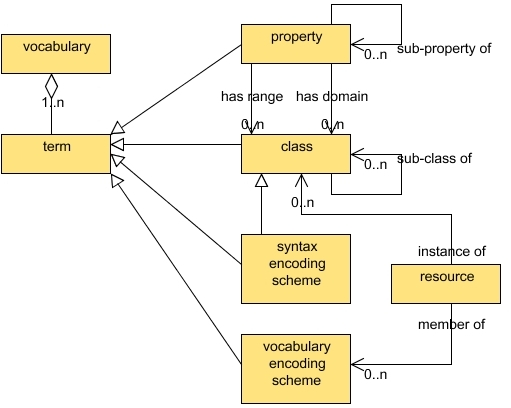
\includegraphics[width=0.6\textwidth]{images/vocabulary-model.jpg}
\caption{Modèle général du DCMI}
\label{img:dcmi-voc}
\end{figure}

\paragraph{Modèle général et représentation}
Une des grandes avancées de \pc{DCMI Metadata Terms}, a été la constitution d'une modélisation générale, voir la Figure \ref{img:dcmi-voc}, et l'introduction d'une syntaxe de représentation utilisants XML, RDF et RDF-S. 
En plus des propriétés, le modèle définit la notion de Classe et de Schéma d'encodage (qui sera expliqué ci-après). 
Les classes permettent de définir des types de ressources et de leur attribuer des URI. 

Chaque \pc{Terme} est défini par une liste d'attributs lui donnant un identifiant, une étiquette, une définition, ajoutant des commentaires, de la documentation, une référence complémentaire, les relations hiérarchiques avec les autres Termes, la classe et le type du Terme, l'appartenance à un Schéma d'encodage, les restrictions de sujet et d'objet qui s'applique à une propriété, les propriétés équivalentes.
Ainsi, on peut maintenant utiliser des URI, faisant référence à d'autres ressources, comme valeur d'une propriété.
Les valeurs peuvent donc être soit une expression littérale, une URI quelconque, ou bien une URI pointant vers un type de ressource particulier, comme un Terme appartenant à un schéma d'encodage ou une classe.
Par exemple, la propriété \pc{creator} ne peut pointer que vers des ressources de classe \pc{Agent} (du fait d'une restriction \pc{hasRange}). 


\paragraph{Schémas d'encodage}
Il existe deux types de schémas d'encodage qui permettent de préciser si les valeurs des propriétés sont écrites selon une syntaxe particulière (\pc{Syntax Encoding Scheme}, SES), ou si la valeur fait partie d'un thésaurus ou d'un vocabulaire contrôlé (\pc{Vocabulary Encoding Scheme}, VES).
Cela permet par exemple, d'indiquer que les valeurs de la propriété \pc{date} sont écrites suivant le format du W3C Date Time Format ou bien suivant la norme ISO 8106. 
De même, on peut déclarer que les valeurs de la propriété \pc{subject} seront prises dans la liste des \pc{Library of Congress Subject Headings}. 
%need REF ! 
SES et VES offrent ainsi la possibilité d'utiliser plusieurs jargons ou syntaxes pour caractériser les valeurs des propriétés, voir [A1] dans les besoins de modélisations du chapitre précédent (\ref{sec:bm}).
De plus, la spécification d'un Terme permet d'ajouter une définition et de pointer vers d'autres ressources pour documenter les Termes, voir [A2].

\begin{figure}[ht!]
\centering
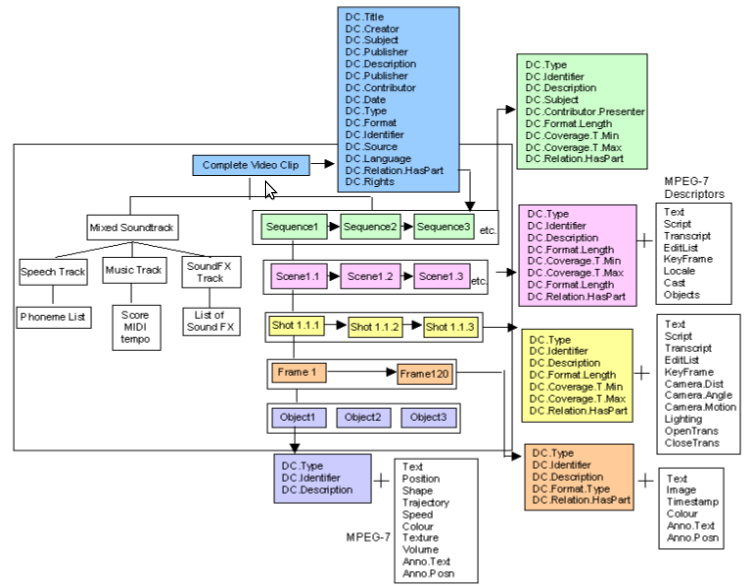
\includegraphics[width=0.8\textwidth]{images/HunterDCMI-MPEG7.png}
\caption{Modèle de Dublin Core étendu pour l'audiovisuel avec des descripteurs MPEG-7 (\cite{Hunter1999})}
\label{img:dcmi-mpeg7}
\end{figure}


\paragraph{Application à l'audiovisuel}
La modélisation du DCMI Metadata Terms s'intéresse à la description de tout type de ressources sur le Web (ce qui est identifié par une URI \cite{Berners-Lee1998}).
Cette perspective très générique lui permet de s'appliquer à de nombreux cas d'usages sans pour autant traiter leurs spécificités. 
Ainsi, dans le cas de l'audiovisuel il faudrait étendre ce schéma pour décrire par exemple le format d'image, les différents contributeurs, inclure de nouveaux types de dates, de nouvelles classes de Termes etc.

\cite{Hunter1998} ont proposé une extension qui raffine les propriétés du Dublin Core et les applique à différents niveaux de composition de l'objet audiovisuel, voire la Figure \ref{img:dcmi-mpeg7}.
Ainsi, l'objet audiovisuel est d'abord décomposé en élément audio (avec des pistes de paroles, de musique et d'effets) et vidéo.
Puis la vidéo est hiérarchisée en séquences, scènes, plans, images et objets dans une image.
À chaque niveau s'applique un ensemble de propriétés, dont des ajouts par rapport au schéma (la Description est lié à une liste de Genre, le Format permet d'indiquer le diffuseur).
\cite{Hunter1999} poursuivent ce travail et propose une représentation de ce schéma pouvant être intégré à MPEG-7. 


\paragraph{Discussion}
L'approche poursuivie par \cite{Hunter1999} est cependant assez contraignante du fait de la décomposition hiérarchique figée et non applicable à tous les types de production audiovisuelle.
En particulier, la notion de séquence et de scène est propre à la production de fiction. 
Les niveaux de hiérarchisation devraient s'adapter aux particularités de chaque type de production. 
De plus, la description des niveaux de fragmentation inférieurs à la séquence repose de plus en plus sur des descripteurs de MPEG-7. 
En effet, le nombre de propriétés de Dublin Core utilisées baisse à chaque niveau de fragmention et on n'utilise plus que trois propriétés pour le dernier niveau (\e{identifier}, \e{type} et \e{description} pour associer les descripteurs MPEG-7).
Ce déséquilibre progressif entre les deux schémas reflète bien leur cadre d'usage. 
Si Dublin Core est particulièrement pertinent pour les niveaux documentaires les plus hauts, sa pertinence diminue quand on rentre dans le détails des fragments audiovisuels.
Il est alors nécessaire de lui adjoindre un schéma de description propre à l'audiovisuel comme MPEG-7.
Finalement, un schéma comme DMS-1 (voir \ref{sec:wrapper}) apparaît comme plus adapté qu'une extension de Dublin Core + MPEG-7 pour couvrir ces besoins.
Et ce, d'autant plus, que DMS-1 fournit des informations plus adaptées à l'audiovisuel (ne serait-ce que l'exemple des titres) et favorise un découpage factuel extensible ainsi qu'une description éditoriale.



%=============
\subsection{MPEG-7 Part 5: Multimedia Description Scheme}\label{sec:mpeg7}
% \cite{Hunter2001} ; \cite{Troncy2007} ; \cite{Nack2005a} ; \cite{Dasiopoulou2009} ; \cite{Garcia2005} ; 

% à revoir
Parmi les normes utilisés pour décrire le contenu des audiovisuels, MPEG-7 est certainement devenu le standard de l'industrie. 
Développé à partir de 1998 par le comité MPEG (Moving Picture Expert Group) à la suite des standards MPEG-1, MPEG-2 (norme de compression du signal audiovisuel) et MPEG-4 (norme de d'encodage multimédia basée sur les objets), MPEG-7 est devenu une norme ISO/IEC en 2001 puis mise à jour jusqu'en 2006. 

La norme définit un ensemble de \e{Descripteurs} (Descriptors, Ds) dont les valeurs permettent de caractériser un objet audiovisuel, qu'il s'agisse de composantes du signal ou bien d'autres aspects comme des informations relatives à sa création, sa structure, son usage passé et futurs etc.
Ces Descripteurs sont organisés en \e{Schémas de Descriptions} (Description Schemas, DSs) dont on peut avoir une vue d'ensemble dans la Figure \ref{img:soa:mds}.
C'est cette partie de la norme (\cite[Part 5 : Multimedia Description Scheme]{ISO/IEC2003}) que nous traiterons en particulier dans cette section. 

\begin{figure}[ht!]
\centering
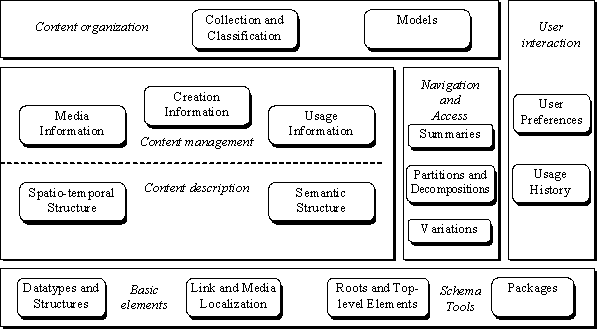
\includegraphics[width=0.8\textwidth]{images/MPEG-7-MDS.png}
\caption{Vue d'ensemble des Schémas de Description (DSs) de la norme MPEG-7}
\label{img:soa:mds}
\end{figure}

Les descriptions produites sont représentées dans un \e{Langage de Description des Définitions} (Description Definition Language, DLL) qui permet de spécifier la syntaxe des Descripteurs, la structure des Schémas de Description ainsi que la sémantique de l'ensemble.
Ce langage permet également de créer ou modifier des Descripteurs, d'étendre ou de modifier les Schémas de Descriptions. 
Le DLL est en réalité XML Schema (\cite{Fallside2004}) agrémenté de quelques types primitifs.

Pour utiliser MPEG-7, il faut également des outils et des directives annexes qui permettent de guider les utilisateurs. 
% définition / implémentation ? 
Dans la partie \e{Systems} de la norme, on trouve ainsi la définition d'outils qui remplissent les fonctions suivantes : codage d'une description MPEG-7 en binaire ; mécanismes de transmissions des descriptions (en binaire ou en texte) à part ou en parallèle du contenu audiovisuel décrit ;  synchronisation entre description et contenu audiovisuel ; gestion des descriptions et de la propriété intellectuelle. 
La partie \e{Reference Software} présente des logiciels de références pour utiliser la norme.
Enfin, la partie \e{Conformance} explicite des directives et des procédures pour s'assurer de la conformité des descriptions produites.

Nous détaillerons dans cette section les Schémas de Description liés à la gestion du contenu (\e{Content Management} dans la Figure \ref{img:soa:mds}) et à la description du contenu (\e{Content Description}).\\


\subsubsection{Gestion du contenu}
MPEG-7 définit trois concepts fondamentaux pour modéliser l'enregistrement d'une réalité en un contenu multimédia et les multiples transformations qu'il est possible de lui appliquer. 
Ainsi, pour chaque modalité d'enregistrement (audio, audiovisuel, photo etc.) MPEG-7 considère la création de trois éléments, une \pc{ContentEntity} (entité de contenu, CE), une \pc{MediaInstance} (instance de média, MI) et un \pc{MediaProfile} (profil de média, MP), voir la Figure \ref{img:soa:media}.
Pour donner une première idée, on peut dire que le fichier créé correspond à la \pc{MediaInstance}, que le \pc{MediaProfile} correspond aux paramétrages de son encodage et que la \pc{ContentEntity} représente le contenu de manière abstraite.

\begin{figure}[ht!]
\centering
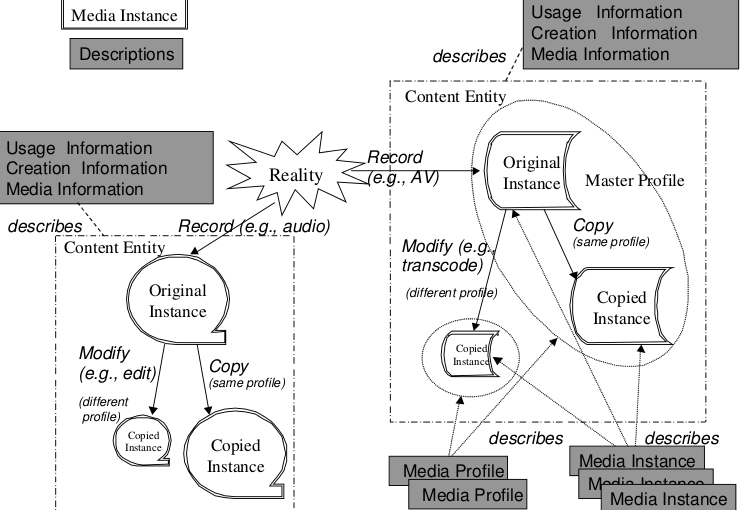
\includegraphics[width=0.8\textwidth]{images/MPEG-7-MediaManagement.png}
\caption{Gestion des contenus dans MPEG-7 à trois niveaux : contenu, instance et profile.}
\label{img:soa:media}
\end{figure}


On remarque qu'il existe cependant des différences entre les \pc{MediaInstance}, entre l'original et ce qui est nommé des \gui{copies} (copied instances). 
Ce qui est particulièrement intéressant pour nous est de constater que la nature de la manipulation entre l'original et les soi-disantes \gui{copies} importe peu (copie technique, réencodage ou montage), car cela crée de toute façon une nouvelle \pc{MediaInstance}. 

À l'inverse, la notion de \pc{MediaProfile} est dépendante de la nature de ces transformations. 
Le \gui{MasterProfile} correspond ainsi aux paramètres d'encodage de la MI d'origine, la première créée. 
Ainsi, dès qu'une différence d'encodage apparaît avec les MI créées ultérieurement, un nouveau \pc{MediaProfile} est créé. 
Il correspond donc à un regroupement de toutes les instances ayant en commun le même encodage. 
%%%% orthographe %%%%
Ce qui paraît troublant néanmoins, est l'amalgame fait entre réencodage et montage. 
Les changements de structure réalisés par le montage semblent en effet bien plus significatif qu'un changement de paramètre d'enregistrement. 
On peut se souvenir de la citation d'\pc{Eisenstein} à ce sujet évoqué en section \ref{sec:prod}.

Enfin, la notion de \pc{ContentEntity} correspond à une entité abstraite permettant de regrouper toutes les versions ultérieures de ce même contenu.
De ce fait, c'est à elle qu'on attache des informations concernant la création, l'usage et le type de média construit. % ??? Sûr ???
Ce regroupement d'informations à ce niveau découle de l'idée que chaque \pc{ContentEntity} définit une forme reconnaissable de contenu, quelque soit les variations apportées.
Encore une fois, l'idée qu'un montage différent n'impacte pas la forme et donc potentiellement l'identité du contenu nous semble ambiguë. 
Il s'agit là d'un de nos points d'achoppement par rapport à la modélisation proposée par la norme. 

\paragraph{Schémas de description}
Détaillons maintenant les trois Schémas de Descriptions proposés par MPEG-7 dans la partie \gui{Content Management}.
Remarquons que ces schémas s'appliquent tous à décrire les \pc{ContentEntity}.
% plus de détails sur les DSs

Le \pc{MediaInformation} est un schéma qui comporte des informations d'identification du CE ainsi qu'un ou plusieurs Profiles d'instances. 
Il faut remarquer que la définition du Profile proposé implique que le moindre changement d'encodage aboutit à la création d'un nouveau Profile en plus de l'instance. 
Il devient alors clair qu'un Profile représente la description d'un groupe d'instances, dont il facilite la gestion.
\begin{liste}
	\item \pc{MediaIdentification} : propose un ou plusieurs identifiants pour le CE.
	\item \pc{MediaProfile} : est composé de plusieurs descripteurs qui détaillent les paramètres et formats utilisés pour encoder une ou plusieurs instances.
	Il s'agit en particulier du \pc{MediaFormat} (pour l'encodage et le format d'encapsulation des données) ; le \pc{MediaInstance} (visant à identifier et localiser les instances) ; le \pc{MediaTranscodingHints} (pour faciliter le réencodage des données) ; le \pc{MediaQuality} (pour détailler la qualité et les défauts). 
\end{liste}


Le \pc{CreationInformation} peut être considéré comme une version étendue à l'audiovisuel des éléments du DCMI. Il comporte les Schémas de Description suivants : 
	\begin{liste}
		\item \pc{Creation} : des métadonnées qui permettent d'identifier le contenu (titre), proposer un résumé et des informations sur les conditions de sa création (créateur et contributeurs avec leur rôle, lieu, date, matériel et paramètrage utilisé).

		\item \pc{Classification} : des éléments de classification du contenu par forme (film, journal télévisé etc.), genre (sport, politique etc.), sujet, langage présent, et des informations sur la diffusion (date, région, public cible, critiques etc.)

		\item \pc{RelatedMaterial} : des métadonnées sur les autres versions d'un même contenu (format, type de média, localisation du média etc.) qui sont ensuite elles-mêmes décrites comme des éléments à part.
	\end{liste}

Le \pc{UsageDescription} est un schéma qui comporte un descripteur détaillant les droits attachés au contenu (\pc{Rights}), un descripteur décrivant les résultats financiers (\pc{FinancialResults}) et des schémas de descriptions sur les détails d'utilisation du contenu (\pc{Availability}) et sur l'historique de son utilisation(\pc{UsageRecord}).
Les droits d'exploitation peuvent en effet porter uniquement sur certains types de distribution (DVD, télédiffusion etc.) ou une certaine période. 
L'historique permet de garder trace des diffusions et de leur audience.


\subsubsection{Description du contenu}
\paragraph{La structure spatio-temporelle du contenu}
MPEG-7 fournit un ensemble de schémas et de descripteurs qui permettent de découper les contenus multimédias de toute les manières possibles. 
Pour cela, la norme définit la notion de \pc{Segment} qui se décline en segment spatial, temporel ou spatio-temporel et sur tout type de média (audio, image, audiovisuel, multimédia). 
Chaque segment peut se décomposer en d'autres segments suivant la structure d'un arbre. 
De plus, ces segments peuvent être connectés entre eux ou pas, c'est-à-dire spécifier trois zones connexes ou pas d'une image ou bien trois séquences temporelles qui se suivent ou pas. 
Les Segments peuvent également n'être valable que pour une source média particulière, comme une piste audio comportant la musique.

Un point particulièrement important est que chacun de ces \pc{Segment} est considéré comme une \pc{ContentEntity}. 
On peut donc utiliser les schémas de \pc{MediaInformation}, \pc{CreationInformation} et de \pc{UsageDescription} pour les décrire ainsi qu'un schéma \pc{Semantic} que nous décrivons ci-après. 
En plus de cela, de nombreux schémas spécifiques à la nature du média existent pour décrire le signal de manière analytique. 


\paragraph{Aspects sémantiques}
Le schéma \pc{Semantic} permet de décrire le monde qui est présenté aux lecteurs dans le contenu audiovisuel. 
Il s'agit d'une description basée sur les évènements (\pc{Event}) ayant lieu à tel moment (\pc{SemanticTime}), à tel endroit (\pc{SemanticPlace}), et auxquels participent des objets (\pc{Object}) ou des agents (\pc{AgentObject}). 
La description peut être raffinée en utilisant des concepts (\pc{Concept}), en détaillant les attributs d'une entité (\pc{SemanticState}) ou bien les relations entre entités (\pc{SemanticRelation}).
À noter, que ces relations peuvent tout autant porté sur les évènements se déroulant dans le contenu (par exemple, l'agent A est bénéficiaire d'un évènement B) ou bien entre un contenu et des entités sémantiques (par exemple, l'image A est une référence à l'objet B).

% VariationDescription !!!!







%Core Ontology for MultiMedia
%=============
\subsection{Ontologies basées sur MPEG-7}\label{sec:mpeg7etc}
% \addcontentsline{toc}{subsubsection}{Core Ontology for MultiMedia}
MPEG-7 est une norme qui propose de nombreux descripteurs pour modéliser les objets audiovisuels.
La grande force de son approche est d'associer ces descripteurs à n'importe quelle séquence de contenu multimédia.
Cette richesse amène également une certaine difficulté dans l'appréhension de sa modélisation, tant la norme est étendue et complexe. 
De nombreux auteurs ont critiqué l'approche de représentation de la norme, notamment du fait de l'ambiguïté sémantique et syntaxique des descriptions produites (\cite{VanOssenbruggen2004, Nack2005a, Troncy2007, Dasiopoulou2009, Arndt2007}).

En effet, si l'utilisation des langages XML semblait légitime à l'époque, il en résulte un manque de formalisation qui complique les raisonnements et l'interopérabilité avec d'autres schémas de description (\cite{Nack2005a}).
De plus, la possibilité de créer plusieurs variantes syntaxiques valides pour représenter la même description rend difficile leur maintien et leur intéropérabilité, et ce même avec d'autres descriptions MPEG-7 (\cite{Arndt2007}).
Une approche formalisée sémantiquement aurait permis de réconcilier ces différentes variantes de représentation. 

Deux autres inconvénients mis en évidence par \cite{Nack2005a} sont la rigidité structurelle des descriptions et l'abscence de relations entre documents. 
La description d'un fragment de contenu ne peut se faire hors d'une structure de description d'un document entier. 
Une fois cette structure fixée, elle ne pourra plus être altérée, sous peine de la rendre incompatible avec les anciennes versions.
Les relations doivent également être contenu à l'intérieur d'une description d'un document.
De ce fait, créer une relation entre deux programmes obligent à créer un document de type collection contenant ces deux programmes.

MPEG-7 reste une source de référence et d'inspiration pour plusieurs série de travaux qui tentent de pallier ces défauts de représentation.
Leur approche consiste à proposer une formalisation sémantique d'une partie du standard avec pour objectif de relier ces descriptions à des ontologies de domaine.
\cite{Troncy2007} et \cite{Dasiopoulou2009} ont étudié plusieurs de ces travaux en vue de les comparer, voir la Table \ref{tab:ontos} pour une synthèse de leur comparaison. 
Dans la suite de la section, nous présentons chacun de ces travaux avant de faire le point sur leur stratégies respectives d'intégration à des ontologies de domaine.
Enfin, nous discutons des apports et des manques de ces ontologies par rapport aux besoins que nous avons exprimés en début de chapitre (\ref{sec:bm-av}).

Ces travaux se distinguent de plusieurs manières : 
\begin{liste}
	\item par l'étendue de leur reprise de \g{MPEG-7} (colonne éponyme).
	On remarquera en particulier que ces ontologies se concentrent sur les parties de décomposition structurelle des objets audiovisuels (Structure), et sur les descripteurs bas-niveau (Visual DS et Audio DS).
	\item l'ontologie générique à laquelle il se raccroche (colonne \g{Ontologie}) 
	\item la conceptualisation utilisée pour réaliser des alignements et des liens avec des ontologies de domaine (colonne \g{Intégration}) 
	\item le type et le domaine d'applications visés (colonne \g{Applications}) 
	\item le langage de représentation utilisé (RDF-S ou OWL) (colonne \g{Langage}) 
	\item le type de modélisation, modulaire (fond blanc) ou monolithique (fond gris).
\end{liste}

\begin{table}[htb!]
% \begin{center}   			{l p{61pt} p{60pt} p{130pt} r}
							% {l p{55pt} p{35pt} p{55pt} p{130pt} r}
\begin{tabularx}{\textwidth}{|l|p{61pt}|X|X|p{130pt}|r|}
\hline
	\g{Nom} & \g{MPEG-7} & \multicolumn{2}{c|}{\g{Ontologie}~|~\g{Intégration}} & \g{Application} & \g{Langage} \\ \hline\hline
	
	\rowcolor{lightgray}
	\pc{Harmony} &  Structure+ Visual & \multicolumn{2}{>{\columncolor{lightgray}}c|}{ABC} & analyse et annotation d'image dans le milieu médical & OWL Full \\ \hline
	
	\pc{aceMedia} & Structure+ Visual& \multicolumn{2}{c|}{DOLCE Lite+ AO} & analyse et annotation de match de tennis & RDF-S \\ \hline

	\pc{SmartWeb} &  Structure+ Visual & \multicolumn{2}{c|}{SmartSUMO} & analyse et annotation de vidéo de match de football & OWL \\ \hline

	\pc{Boemie} & Structure+ Visual+Audio & -- & Boemie & analyse, annotation et recherche de documents multimédia & OWL-DL  \\ \hline
	
	\pc{COMM} & Structure+ Visual & \multicolumn{2}{c|}{DOLCE} & gestion de documents multimédia pour l'industrie & OWL-DL \\ \hline

	\rowcolor{lightgray}
	\pc{Rhizomik} & MPEG-7 en entier & -- & Semantic DS & conversion MPEG-7 XML vers OWL & OWL-DL \\ \hline

	\pc{DS-MIRF} & MDS complet & -- & Semantic DS & conversion MPEG-7 XML vers OWL (football et formule 1) & OWL-DL \\ \hline
\end{tabularx}
\caption{Synthèse des ontologies basées sur MPEG-7}\label{tab:ontos}
% \end{center}
\end{table}



\paragraph{\pc{Harmony}}
\cite{Hunter1999} ont réalisé la première tentative de formalisation sémantique de MPEG-7. 
L'ontologie \pc{Harmony} était représentée initiallement en RDF-S puis en OWL Full, et suit de près la modélisation proposée par MPEG-7. 
Il en résulte les mêmes constats que pour MPEG-7, la modularité des descriptions ainsi qu'une ambiguïté syntaxique et sémantique.

Les travaux de \cite{Hunter2001} ont intégré l'ontologie générique ABC permettant de modéliser des temporalités (évènement, situation, action), des actualités (artefact ou agent) et des oeuvres.
L'intégration d'ABC doit aussi permettre de créer des relations ou des alignements avec des ontologies génériques ou de domaine, pour favoriser l'interopérabilité la spécialisation des descriptions. 
\cite{Hunter2004} est un exemple d'utilisation de l'ontologie pour l'annotation et l'analyse d'images médicales. 


\paragraph{\pc{aceMedia}}
Le projet \pc{aceMedia}\footnote{http://www.acemedia.org} a développé deux ontologies basées sur MPEG-7. 
La \pc{Multimedia Structure Ontology} (MSO) pour la description de la structure des objets audiovisuels, et la \pc{Visual Descriptor Ontology} (VDO) pour les aspects visuels (\cite{Petridis2004, Martinez2002}).
Ces ontologies proposent une modélisation modulaire, proche de MPEG-7, mais qui clarifie certaines ambiguïtés syntaxiques, à l'inverse d'\pc{Harmony}.
Par exemple, MSO introduit les classes \cd{mso:Frame} et \cd{mso:KeyFrame} afin de distinguer leur rôle respectif. 
Dans MPEG-7 et \pc{Harmony}, la description d'une image pouvait résulter de l'utilisation d'un \pc{VideoSegment} ou d'une \pc{StillRegion}.

MSO et VSO utilisent deux ontologies génériques, DOLCE Lite et l'Annotation Ontology (AO).
L'AO a été construite pour spécialiser les entités de DOLCE (\cite{Borgo2002}) afin de faciliter la mise en relation avec des ontologies de domaine.
Ces ontologies ont été utilisé pour l'analyse et l'annotation d'images et de vidéos dans le domaine du sport (jeu de tennis, \cite{Petridis2006}) et pour des vidéos personnelles.


\paragraph{\pc{SmartWeb}}
Le projet \pc{SmartWeb}\footnote{http://www.smartweb-projekt.de/start\_en.html} a permis de développer un ensemble d'ontologies pour construire des services d'in\-fo\-rmation sur le Web. 
Parmi cet ensemble, on trouve une ontologie d'annotation de contenu multimédia qui se construit sur l'ontologie générique SmartSUMO (\cite{Oberle2007, Vembu2006}).
SmartSUMO est elle-même développée dans ce projet à partir de DOLCE (\cite{Borgo2002}) et SUMO (\cite{Niles2001}). 
Par rapport aux deux premières ontologies, celle-ci permet d'ajouter des informations de création et de production en formalisant le processus d'annotation lui-même.

Une particularité de la modélisation est de considérer les objets multimédia et les segments comme deux classes soeurs, et non comme une spécialisation, ce qui amène certaines ambiguïtés dans des décompositions complexes.
L'ontologie a été utilisée pour l'analyse et l'annotation de vidéos de match de football.


\paragraph{\pc{Boemie}}
Le projet \pc{Boemie}\footnote{http://www.boemie.org/} a permis de développer deux ontologies ; la \pc{Multimedia Content Ontology} (MCO) et la \pc{Multimedia Descriptors Ontology} (MDO). 
Ces ontologies visent à re-modéliser MPEG-7 en OWL-DL, du point de vue de la décomposition des objets audiovisuels et des descripteurs audio et vidéo de bas-niveau (\cite{Dasiopoulou2009a}).

On retrouve la séparation entre objets audiovisuels et segments, mais cette modélisation utilise des restrictions de classes pour éviter toute ambiguïté.
La décomposition peut également se faire de manière indépendante sur un plan logique (unité logique) et factuel (segments).
Le lien avec des ontologies de domaine se fait par des relations pointant vers des concepts génériques de MCO.
\cite{Karkaletsis2005} proposent une utilisation de ces ontologies dans le cadre de l'analyse, l'annotation et la recherche de documents multimédia.


\paragraph{COMM}
La \pc{Core Ontology for MultiMedia} (COMM) est la tentative la plus récente de formalisation de MPEG-7 (\cite{Arndt2007, Staab2008, Arndt2009}).
Ce travail permet de spécialiser au domaine de l'audiovisuel les patrons de conception (Design Pattern) suivants : \pc{Descriptions \& Situations} (D\&S) et \pc{Ontology of Information Objects} (OIO) de DOLCE (\cite{Gangemi2005}).
COMM retravaille la modélisation de MPEG-7 pour la formaliser et la rendre modulaire. 

COMM définit 4 patrons ; la \e{décomposition structurelle} d'un objet en segments multimédia ; l'\e{annotation de contenu} qui permet d'associer des informations à un objet ou un segment ; l'\e{annotation du média} qui décrit les fichiers multimédias, leur encodage etc. ; l'\e{annotation sémantique} qui permet d'associer les objets ou segments multimédias avec des éléments d'ontologies de domaine. 
Une des particularités de COMM est de formaliser le processus d'annotation, mais pas tout à fait de la même manière que les ontologies de \pc{SmartWeb}.
L'annotation est ici le résultat d'une méthode d'annotation (manuelle, automatique), dont on peut décrire les paramètres, et qui sert de lien entre l'élément annoté et l'annotation sémantique.

L'ontolgoie COMM a été utilisée pour la gestion de documents multimédia dans des applications industrielles (comparateur de voitures, gestion de problèmes moteur pour l'aéronautique).
Si COMM clarifie la modélisation de MPEG-7, l'utilisation de DOLCE tend également à la complexifier.
Ainsi, une API\footnote{http://multimedia.semanticweb.org/COMM/api} Java a été développée pour cacher cette complexité et faciliter la création de descriptions et l'implémentation de services de recherche.



\paragraph{\pc{Rhizomik}}
Contrairement aux approches précédentes, \cite{Garcia2005} ont developpé une méthode de conversion automatique de MPEG-7 dans le cadre du projet \pc{ReDeFer}\footnote{http://rhizomik.net/redefer}.
Alors que les autres approches retravaillent la modélisation de MPEG-7 pour la clarifier et l'ajuster à leurs besoins, cette méthode reprend directement le XML Schema du standard.
La méthode repose sur deux langages d'alignement, XML2RDF et XML2OWL qui permettent de convertir tous les éléments en une ontologie OWL nommée \pc{Rhizomik}.

La séparation entre objets et segments multimédia est totale puisque les deux classes ne sont même pas soeurs.
De plus, reprenant MPEG-7, cette nouvelle représentation conserve les défauts déjà mentionnés : ambiguïté et complexité.
Du point de vue de la mise en relation avec des ontologies de domaine, cela est rendu possible par l'intermédiaire du Semantic DS.
Cette modélisation (décrite en \ref{sec:mpeg7}) est plus orienté et moins complète que celle proposée par des ontologies génériques.
De plus, l'approche nécessite d'utiliser un XML Schema pour définir les concepts du domaine, avant de pouvoir effectuer la transformation en une ontologie OWL.
De ce fait, l'ontologie est mieux utilisée pour transformer des descriptions MPEG-7 que pour faciliter l'intégration avec d'autres ontologies.


\paragraph{DS-MIRF}
\cite{Tsinaraki2004a, Tsinaraki2007} présentent le DS-MIRF framework qui traduit manuellement le MDS, l'Audio DS et le Visual DS en une ontologie OWL-DL.
Plus précisément, la transformation est pilotée par une ontologie tierce qui définit les alignements en le XML Schema et les entités OWL.
Cette méthode permet d'expliciter et de clarifier certaines ambiguïtés de MPEG-7, mais la structure de l'ontologie reste proche de celle de \pc{Rhizomik}.

Une méthodologie a été proposée pour traduire systématiquement les déclarations réalisées avec une ontologie de domaine en déclarations compatibles avec la sémantique de MPEG-7.
Ainsi, contraiment à la méthode de \pc{Rhizomik}, l'intégration avec d'autres ontologies est réalisé en définissant un alignement, plutôt qu'en transformant les ontologies en XML Schema.
Le DS-MIRF framework a été utilisé pour l'annotation de match de football et de courses de Formule 1.


\paragraph{Stratégies d'intégration à des ontologies de domaine}
En guise de synthèse, nous comparons les stratégies d'intégration des ontologies basées sur MPEG-7 avec des ontologies de domaine.
Ces ontologies de domaine servent à produire des descriptions sur le contenu d'objets ou segments multimédia, en proposant des concepts et des propriétés spécifiques à ce domaine. 
Nous avons vu que de nombreux exemples d'applications s'intéressent à un domaine sportif (football, tennis etc.).
Cela permet alors d'enrichir la description, essentiellement techniques, de ces objets et de proposer une indexation propre à un métier.
Les ontologies présentées mobilisent trois stratégies : 
\begin{liste}
	\item \e{l'utilisation d'une ontologie générique} pour faire le lien entre les objets multimédias et des descriptions issues de l'ontologie de domaine. 
	C'est le cas de l'ontologie \pc{Harmony} avec ABC, des ontologies du projet \pc{aceMedia} et \pc{Boemie}.
	L'ontologie générique fournit des classes génériques que l'ontologie multimédia et de domaine peuvent spécialiser. 
	Ces classes sont reliées par des propriétés génériques, et spécialisables, qui permettent de relier un objet multimédia avec des déclarations de l'ontologie de domaine.
	Dans ce cas, l'intégration entre les ontologies dépend fortement de l'architecture de l'ontologie générique.

	\item \e{l'utilisation du Semantic DS}, moins complet et plus orienté que les ontologies génériques.
	C'est le cas des ontologies \pc{Rhizomik} et DS-MIRF, même si elles n'utilisent pas tout à fait la même méthodologie (voir leur présentation) pour faire l'intégration.

	\item \e{une formalisation de la méthode de création des liens} en plus de la formalisation des liens entre objets multimédia et descriptions sémantiques. 
	C'est l'approche utilisée dans COMM et les ontologies de \pc{SmartWeb}.
\end{liste}

Enfin, il est important de noter que dans les approches utilisant des ontologies génériques, la modélisation des objets audiovisuels est indépendante de la stratégie d'intégration à des ontologies de domaine. 
Ainsi, il serait possible d'utiliser la dernière approche dans \pc{Harmony}.

\paragraph{Discussion}
[\g{B1 : autonomie}]
[\g{B2 : réutilisabilité}]
%  structure documentaire générique, extensible ?
%  description propre à la prod. av ? le signal tend mais n'y est pas encore
% intégration avec des ontos de domaine importante, bcp d'efforts pour des formalismes de haut-niveau, mais du coup difficile à appréhender par les utilisateurs, problème d'adoption ?
% peu de lien avec le contexte, approche a posteriori qui ne permet pas de prescription ou de description au fil de la production




%=============
\subsection{Ontology for Media Resources}
Suite aux travaux du W3C Media Annotation Working Group (MAWG), \cite{Burger2011} puis \cite{Lee2012} ont développé une ontologie minimaliste pour décrire et rechercher des informations sur des ressources média sur le Web.

\begin{figure}[ht!]
\centering
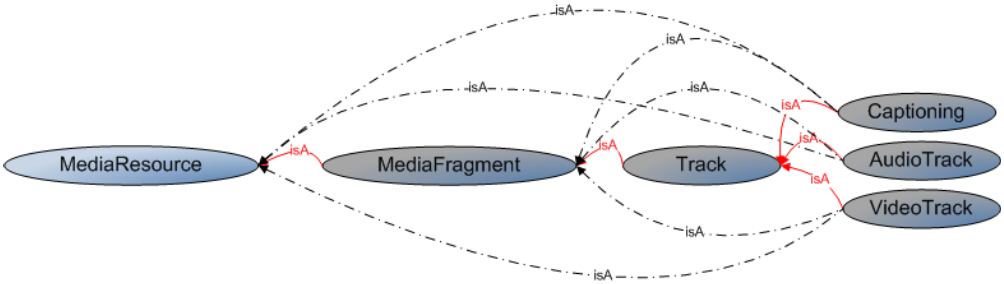
\includegraphics[width=0.8\textwidth]{images/MA-model.png}
\caption{Hiérarchie de classes sous le concept de \pc{MediaResource}}
\label{img:ma-model}
\end{figure}

La modélisation repose sur les concepts de \pc{Collection}, \pc{MediaResource}, \pc{MediaFragment}, \pc{Track} et \pc{Image}, voir la Figure \ref{img:ma-model}.
La décomposition des objets multimédia se fait donc par des fragments, que l'on peut ensuite décomposer en piste et en image.
Cette simplicité apparente, comparée aux approches de segmentation complexe de MPEG-7, cache en réalité l'utilisation d'une autre recommandation du W3C.
La définition d'un MediaFragments peut se faire à partir de l'URI de son média source, où l'on ajoute un syntaxe de décomposition (\cite{Hausenblas2011}).
Par exemple, l'url suivante \cd{http://www.example.com/example.ogv\#t=10,20} désigne le fragment temporel commençant à 10s. et finissant à 20s.
La décomposition peut se faire selon une dimension spatiale, temporelle, en pointant une piste de la source, en pointant un autre fragment prélablement identifié, ou bien n'importe quelle combinaison de ces dimensions.
Des informations techniques (encodage, durée, format etc.) peuvent également être associée aux ressources.

En plus de ces classes, on trouve dans l'ontologie le concept d'\pc{Agent} (personne ou organisation), de \pc{Location} (lieu), de \pc{Genre} (le genre de programme suivant un dictionnaire spécialisé), de \pc{Rating} (permettant d'enregistrer les évaluations de lecteurs/spectateurs) et de \pc{TargetAudience} (indiquant le public visé par la ressource).
Ces classes supplémentaires permettent d'ajouter des informations sur le contexte de création (qui a participé, où) et de faciliter la diffusion et la recherche de ressource (genre, note, public cible etc.).

\begin{figure}[ht!]
\centering
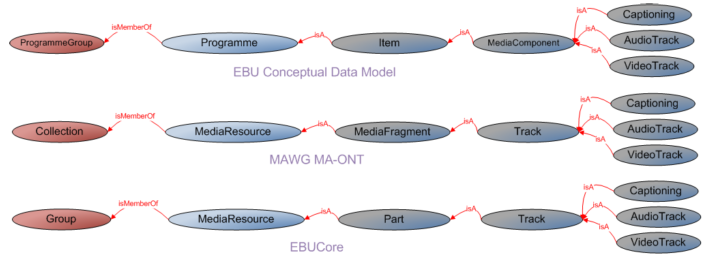
\includegraphics[width=\textwidth]{images/MA-alignement-A.png}
\caption{Alignement avec des ontologies multimédia (partie 1)}
\label{img:ma-alignement-A}
\end{figure}

\paragraph{Alignement avec d'autres conceptualisations}
Un apport important de cette ontologie réside dans le travail d'alignement avec les autres modélisations multimédia. 
Les Figures \ref{img:ma-alignement-A} et \ref{img:ma-alignement-B} présentent un alignement minimaliste des principales classes de l'\pc{Ontology for Media Resource}.
Dans la définition de \cite{Lee2012}, les alignements sont étendus à d'autres conceptualisations ainsi qu'aux propriétés de schémas de métadonnées et métadonnées embarquées dans des formats conteneurs.
Ainsi, on se rend compte que ces classes principales, qui représentent une collection d'objets multimédia, un objet, ses fragments et ses pistes de contenu, se retrouvent dans toutes ces modélisations. 
Les variations se situent à la fois dans la manière de découper/segmenter cet objet en fragment (dimension spatiale, temporelle etc.), de le lier aux média et dans la manière et la nature des informations que l'on peut leur associer.

\begin{figure}[ht!]
\centering
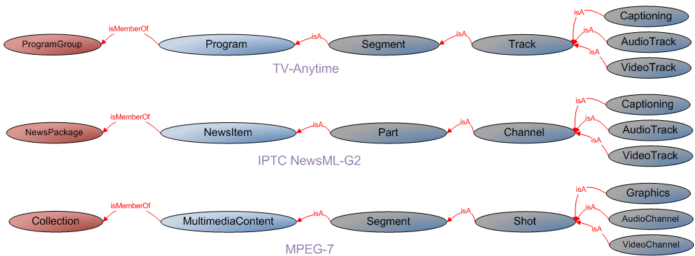
\includegraphics[width=\textwidth]{images/MA-alignement-B.png}
\caption{Alignement avec des ontologies multimédia (partie 2)}
\label{img:ma-alignement-B}
\end{figure}

\paragraph{Discussion}
L'\pc{Ontology for Media Resource} (OMR) a été construite dans un souci de clarté, de cohérence et d'extensibilité et s'intégre particulièrement bien avec les autres recommandations du W3C, dont le Media Fragment URI et SKOS.
L'objectif étant (1) de pouvoir publier des déclarations sur le web de données et (2) construire des systèmes de recherche de contenu interopérables. 
En effet, le travail réalisé sur les alignements permet d'extraire et traduire les informations contenues dans les dépôts n'utilisant pas les mêmes modèles.
Une API\footnote{http://www.w3.org/TR/2010/WD-mediaont-api-1.0-20100608/} a également été construite pour faciliter ces opérations et le déploiement de service de recherche et d'aggrégation de résultats provenant de ces différentes sources.

L'ontologie OMR ne se positionne donc pas comme un supplément de modélisation, mais plutôt comme un travail de synthèse et de mise en correspondance des travaux existants dans une représentation standardisée.
Son objectif n'est pas l'exhaustivité de la représentation des objets audiovisuels ou bien de leur description, mais bien de mettre en commun l'ensemble des informations dispersées et cloisonnées dans les dépôts.





%=============================
%=============================
\subsection{Descriptions métiers basées sur le plan}\label{sec:plan}
Script, Storyboard (\cite{Martin2005}, \cite{ThiBui2003}) etc.
Réappropriations dans le champ informatique : \cite{Chakravarthy2009b} ; \cite{Chakravarthy2009c}

Another trail of research has emerged recently. 
In comparison to the previous approach, it does not attack the multimedia description from below (with signal processing techniques) but from above. 
The principles is to represent the knowledge included in documents related to the multimedia content. 
It can be a web-page where the image is published and commented by others \cite{Simperl2009} or more specific documents related to the production context. 
\cite{Chakravarthy2009b} and \cite{Chakravarthy2009c} take interest in the knowledge of film direction. 
They propose a semantic model which captures the information typically included in a storyboard or screenplay. 
They also provide a system to capture the director's demands and assist her/him during the shooting. 
A similar work has been carried out by \cite{VanRijsselbergen2009} but with distinct goal and language. 
Their MovieScriptMarkupLanguage (MSML) captures the information of a shooting script with a particular attention to the details of set equipment's and actor's positions. 
The related Scoop system \cite{Cardinaels2008} provides its user 3D model of the set as well as the shots taken by the camera in a given position and settings. 
The overall objective is to provide an shooting-set 3D simulation to assist the production team in their preparation.\\





% Our approach follows this trend of research with different focus and objectives than the works presented. We consider the shooting script as the main production document to describe the video shots. The focus is on the realization of these shots, not the preparation or direction of the production. It does not assist the same people and do not provide exactly the same pieces of information. As we demonstrated above, a Semantic Script can assist the cameraman at shooting time and the professional editor when reviewing. 
% In comparison to the COMM ontology, our model offers an additional representation layer with describe the editorial structure of audiovisual objects (Opus, MediaAsset, EditorialObject). With the Semantic Script, we provide a way to predefine a structure and capture intentions that are inherent to the audiovisual production process. COMM represents a MPEG-7 flavored description of video files and also the way this description has been produced by human or algorithms. This indexing is made after the video production and do not provide any mean to retain information from the context of production.


\subsection{Discussion}
[\g{B1 : autonomie}]
[\g{B2 : réutilisabilité}]

%=============
\paragraph{MPEG-21}
% \addcontentsline{toc}{subsubsection}{MPEG-21}
% \cite{Burnett2003} ; \cite{Garcia2010} ? 
%Creation Value Chain
Along with MPEG-7, the MPEG-21 Multimedia Framework \cite{Burnett2003} offers a valuable perspective on future practices in content management, distribution and consumption. The recent interest in content value chains modeling presented in \cite{Garcia2010} shows some similarities with our audiovisual object modeling approach. There is still an open debate about the modeling of the various forms or facets that content can take during its production. Many approaches rely on, adapt or extend the original FRBR Group 1 concepts of \e{Work}, \e{Expression}, \e{Manifestation} and \e{Item}. 
For instance, the Media Value Chain Ontology (MVCO) \cite{Rodriguez-Doncel2009}, \cite{Rodriguez-Doncel2010} is included as the Part 19 of the MPEG-21 standard. 
The authors merge the concepts of Expression and Manifestation. Moreover, they also propose a new concept of Product for asset which needs to be licensed before publishing. 
% Citer également : Jane Hunter -- Reconciling MPEG-7 and MPEG-21 Semantics through a Common Event-Aware Metadata Model




%=============
\paragraph{TV Anytime}
% \addcontentsline{toc}{subsubsection}{TV Anytime}
\cite{Evain2000} ; \cite{Tsinaraki2004} ; \cite{Tsinaraki2005}



% % \cleardoublepage




% %%%%%%%%%%%%%%%%%%%%%%%%%%%%%%%%%%%%%%%%%%%%%%%%%%%%%%%%%%%%%%%%%%%%%%%%%%%%%%%%%%%%%%%%%%%%%%%%%%%
% %%%%%%%%%%%%%%%%%%%%%%%%%%%%%%%%%%%%%%%%%%%%%%%%%%%%%%%%%%%%%%%%%%%%%%%%%%%%%%%%%%%%%%%%%%%%%%%%%%%
\part*{Contribution}
\addcontentsline{toc}{part}{Contribution}
\chapter{Approche et modélisation}\label{chap:mod}

\e{
L'objectif de la partie \g{Contribution} est de présenter notre conceptualisation et sa représentation informatique dans le cadre plus général d'une approche de description des documents audiovisuels contributive et qui suit le déroulement de la production audiovisuelle, même dans des cas de réutilisation et de production collaborative impliquant des communautés de professionnels ou d'amateurs.
Ainsi, en plus des problèmes de modélisation de la diversité des documents audiovisuels, de leurs différents niveaux de représentation, s'ajoute des problèmes d'échange de connaissances entre contributeurs hétérogènes, qui ne partagent pas les mêmes conceptions, vocabulaires et compétences.
}

\e{
Nous commençons par résumer notre analyse des langages et modélisations étudiés dans les chapitres précédents (\ref{sec:synthese}) pour mettre en évidence les manques des solutions disponibles pour répondre aux problèmes soulevés. 
Cela nous amène à présenter les principes de notre approche qui met en avant la complémentarité des informations produites avant et après la fabrication du matériel audiovisuel (\ref{sec:approche}).
Nous introduisons également l'architecture développée dans le cadre du projet MediaMap pour opérationnaliser cette approche, et notamment les applications nécessaires à son fonctionnement.
Nous présentons en section \ref{sec:axes} une reformulation des verrous scientifiques que nous avons identifiés en section \ref{sec:scien}, ce qui nous permet d'introduire des patrons de conception pour représenter les situations typiques de \e{la} production audiovisuelle (\ref{sec:situations}).
% Ensuite, nous expliquons notre modélisation en introduisant des patrons de conception qui rassemblent les concepts et relations nécessaires à la représentation de situations typiques de la production audiovisuelle (\ref{sec:concept}).
Nous discutons ensuite de la mise en oeuvre de ces patrons (\ref{sec:meo}), qu'il s'agisse de les représenter dans un langage informatique, de donner des exemples d'instanciations ou de spécialisations ou encore de documenter le modèle afin de faciliter l'accès et l'échange des connaissances qu'il exprime.
}


\e{
Dans le chapitre \ref{chap:app}, nous présentons les applications développées par les partenaires du projet MediaMap (\ref{sec:app}) et les expérimentations qui ont été menées avec (\ref{sec:xp}).
Nous présentons finalement notre réflexion sur la validation de notre modélisation, notamment dans le cadre du projet MediaMap (\ref{sec:val}).
% Nous discutons également la représentation de notre conceptualisation avec le langage OWL, notamment en comparant certains de nos choix avec ceux effectués dans SKOS (\ref{sec:op}).
% Finalement, nous argumentons la validité de la modélisation de nos patrons de conception sur le plan informatique et sémantique (\ref{sec:val}).
}

\minitoc

%%%%%%%%%%%%%%%%%%%%%%%%%%%%%%%%%%%%%%%%%%%%%%%%%%%%%%%%%%%%%%%%%%%%%
%%%%%%%%%%%%%%%%%%%%%%%%%%%%%%%%%%%%%%%%%%%%%%%%%%%%%%%%%%%%%%%%%%%%%
%%%%%%%%%%%%%%%%%%%%%%%%%%%%%%%%%%%%%%%%%%%%%%%%%%%%%%%%%%%%%%%%%%%%%
\section{Synthèse de l'état de l'art}\label{sec:synthese}
Dans le chapitre \ref{chap:omod}, nous avons étudié la modélisation de connaissances par les ontologies ainsi que la modélisation des vocabulaires métiers par les terminologies. 
Notre définition des besoins implique d'associer une documentation et une terminologie à notre conceptualisation (\ref{sec:bm}), de manière à faciliter les échanges de connaissances entre tous les contributeurs de la chaîne de production, ainsi que dans les cas de réutilisation où l'on intègre des éléments externes dans sa chaîne.
L'analyse des langages documentaires (\ref{sec:xml}) et de représentation de connaissances (\ref{sec:onto-mc}) montre que leur conception les rend trop généraliste pour couvrir nos besoins spécifiques. 
Nous nous appuyons donc sur leur formalisme pour développer des principes de documentation, qui généralisent les propositions des langages de représentation de thésaurus et vocabulaire structuré (\ref{sec:thesaurus}) à la gestion des jargons métiers.
Ceci nous permet de couvrir nos besoins de représentation et de documentation du vocabulaire propre à la production audiovisuelle, et \e{in fine} d'adapter la forme d'expression des connaissances échangées entre contributeurs hétérogènes.

% Nos objectifs dépassent le cadre de la modélisation documentaire que permet XML et les langages de schéma associés (\ref{sec:xml}).
% Les langages de représentations des connaissances développés par le W3C apportent une formalisation qui permet de clarifier la sémantique de la modélisation et d'envisager la mise en place d'inférences (\ref{sec:onto-mc}).
% Si les langages RDF et RDF-Schema permettent la définition de hiérarchies de classes et de relations, OWL ajoute de nombreux raffinements dont de nouveaux axiomes précisant l'usage des propriétés, ainsi que l'ajout de propriétés d'annotation pour décrire la conceptualisation.
% La version OWL-DL fournit un compromis intéressant entre expressivité et décidabilité, mais ne permet pas de couvrir tous nos besoins [$\delta_1$ : \g{multijargon}].

% Ainsi, nous avons étudié les langages de représentation de thésaurus et vocabulaire structuré (\ref{sec:thesaurus}).
% SKOS et SKOS-XL proposent une représentation minimale et extensible des thésaurus existants, et apporte une formalisation qui permet leur publication sur le Web de données.
% La norme ISO-25964-1 apporte la composition des termes et proposent d'associer plus d'informations sur la création, la maintenance et la documentation du thésaurus.
% Les deux approches se concentrent sur la structuration des concepts auxquels on intègre (SKOS) ou on rattache des termes (dans SKOS-XL et ISO-25964-1, les termes sont définis indépendamment des concepts). 
% Cependant, cette indépendance n'offre pas la possibilité de grouper les termes entre eux afin de modéliser une terminologie métier [$\delta_3$ : \g{évolution, gestion}]. 
% De même, ces modèles définissent des termes préférés qui visent à normaliser l'usage linguistique d'une communauté métier, quelque soit la langue parlée par ses membres.
% Les différences d'usages entre métiers, organisation ou bien entre amateurs et professionnels ne sont pas représentées [$\delta_1$ : \g{multi-jargon}]. 
% La documentation des concepts et des termes correspond tout à fait à nos besoins, en particulier dans SKOS avec la notion de note qui permet de s'adapter à la spécificité de chaque usage [$\delta_2$ : \g{documentation}].\\



Dans le chapitre \ref{chap:mav}, nous avons étudié la manière dont les objets audiovisuels (\ref{sec:dav}) et leur réutilisation (\ref{sec:gest}) étaient envisagées dans différentes communautés.
Il se dégage de cette étude un point de vue centré sur le matériel audiovisuel (le signal) et un autre, documentaire, qui considère l'objet comme une articulation de différentes formes matérielles et sémiotiques. 
Cette approche considère ainsi non pas un objet, mais un document qui prend part à un acte de communication, et dont chacune des dimensions joue un rôle précis. 
% Nous avons mis en avant des divergences et des points aveugles entre les points de vue des professionnels de la production et des communautés scientifiques du multimédia, de l'ingénierie documentaire, de la sémiotique audiovisuelle et des bibliothèques numériques.

Nous nous sommes ensuite intéressés tour à tour à l'étude des formats conteneurs (\ref{sec:wrapper}) et d'autres modélisations des objets audiovisuels.
Le succès des formats conteneurs montre l'importance de l'association d'informations métiers au matériel audiovisuel, pour le déroulement de la chaîne, et l'exploitation de document audiovisuel.
Cependant, on remarque que le format de représentation de ces informations pose un problème d'ambiguïté sémantique et qu'il ne peut être utilisé en début de chaîne, avant la fabrication du matériel.
% L'étude des formats conteneurs nous a montré qu'il était possible de modéliser les objets audiovisuels suivant les perspectives administratives, narratives et documentaires tout en y intégrant le matériel audiovisuel [$\chi_1$ :\g{autonomie}]. 
% Cependant, cette forte intégration ne peut être mise en place qu'à partir de la fabrication du matériel, et vise pas au-délà de sa diffusion.
% De même, l'utilisation d'un format conteneur façonne la modélisation autour de l'objet audiovisuel final, et même s'il embarque des métadonnées sur les fragments, elles ne peuvent être mobilisées pour elle-même.
% Ainsi, la nature même du format oblitère le début de la chaîne et ne permet pas de se concentrer sur des fragments.
% Par ailleurs, nous avons pointé l'ambiguïté sémantique des descriptions associées au matériel audiovisuel [$\chi_2$ :\g{réutilisabilité}].

% \e{
% 	Les formats conteneurs ont montré l'importance de certaines informations pour le déroulement de la chaîne, et l'exploitation de document audiovisuel.
% 	Notre modélisation s'inspire de cette approche et vise à l'améliorer sur les aspects suivants : 
% 	\begin{liste}
% 		\item La modélisation des connaissances associées au document audiovisuel doit pouvoir débuter en début de chaîne, avant même la fabrication du matériel audiovisuel.
% 		\item La modélisation du document audiovisuel et des connaissances associées doit être formalisée pour éviter les ambiguïtés sémantiques ainsi que les problèmes d'appropriation de la part des contributeurs de la chaîne de production.
% 	\end{liste}
% }

Nous avons ensuite examiné des modélisations de l'audiovisuel que l'on a distinguées en deux approches, \e{endogène} et \e{exogène}, que nous jugeons complémentaires. 
Ces approches mettent l'accent respectivement sur la dimension sémiotique ou matérielle des objets audiovisuels (\ref{sec:dav}) sans vraiment les articuler.
% La modélisation \e{endogène} rend compte des connaissances fabriquées en début de chaîne afin de prévoir les étapes suivantes de fabrication du document et du matériel audiovisuel (\ref{sec:insitu}).
% Ces modélisations se rapprochent d'une modélisation documentaire du script, définissant la structure documentaire auctoriale (\ref{sec:pv-id}) et les intentions de mise en forme.
% Cette modélisation du script repose sur une unité de base qui est le plan (introduit dans ce mémoire en \ref{sec:docvoc}).
% Ce découpage est particulièrement intéressant du fait que le plan est à la fois l'élément de base de la narration audiovisuelle (structure documentaire) et l'unité de travail dans le processus de production (description de la fabrication, lien avec le matériel audiovisuel). 
% Il permet ainsi d'associer de multiples connaissances à des fragments audiovisuels. %et facilite ainsi leur réutilisation [$\chi_2$ : \g{réutilisabilité}].
% Le modèle MSML se limite à une représentation XML du script utilisé pour construire une prévisualisation 3D du plateau de tournage ainsi que du résultat filmé (\ref{sec:msml}). 
% Le manque de formalisation sémantique ne favorise pas la transformation de ces informations et leur association avec le matériel audiovisuel effectivement fabriqué [$\chi_1$ : \g{autonomie}].
% L'autre modèle étudié propose une formalisation sémantique ainsi qu'une association entre une description du document et du matériel audiovisuel (\ref{sec:answer}).
% Cependant, ces travaux ne sont pas accessibles et ne peuvent donc être repris ni évalués.
% 
% Les approches \e{exogènes} (\ref{sec:post}) proposent d'analyser le matériel audiovisuel en fin de chaîne. 
% L'approche générique du schéma Dublin Core, même lorsqu'il est spécialisé pour les documents audiovisuels, est surtout pertinente au niveau du document (\ref{sec:dcmi}). 
% La description des fragments n'est ainsi rendue possible que par l'utilisation de descripteurs spécifiques, comme ceux de la norme MPEG-7. 
% De plus, on remarque l'importance d'une structure hiérarchique souple et extensible qui permet de couvrir les nombreux genres de documents produits par la télévision.
% MPEG-7 s'est établie comme une modélisation de référence pour l'audiovisuel (\ref{sec:mpeg7}).
% Pourtant, sa représentation en XML a été largement critiquée pour son ambiguïté syntaxique et sémantique qui a poussé de nombreux chercheurs à développer des formalisations sous la forme d'ontologie (\ref{sec:mpeg7etc}).
% Ces modélisation sont réalisées de manière automatique ou manuelle, et certaines reposent sur une ontologie générique pour favoriser l'intégration avec des ontologies de domaine.
% Au-délà de ces apports, les modèles, comme la norme MPEG-7, adopte un point de vue centré sur le matériel audiovisuel tant au niveau de la gestion que de la description des objets audiovisuels. 
% Ainsi, ils négligent la modélisation de la structure documentaire et manquent de descriptions sémiotiques pertinentes pour la production audiovisuelle atténue l'importance de 
% La gestion se fait au niveau du matériel, par identification d'une source et de variantes plus adaptées à d'autres méthodes de distribution [$\chi_1$ : \g{autonomie}].
% L'abscence de distinction entre des opérations d'encodage et de montage ne permet pas de reconnaître la création d'un nouveau document (ou d'une nouvelle intention de réalisation), mais se limite à reconnaître un nouveau fichier.
% De même, les descriptions sont associées aux fichiers ou bien à des entités qui représentent des ensembles de fichiers ayant des caractéristiques communes [$\chi_2$ : \g{réutilisabilité}]. 
% De plus, si le découpage du matériel en segment permet de créer de multiples structure d'analyse sur l'objet, la caractérisation de ces segments par genre ne suffit pas à modéliser les contraintes de sa grammaire documentaire.
% Il n'y a pas non plus de description du processus de production de ces segments, ni de l'écriture filmique.
% 
% \e{
	La production audiovisuelle et les modèles \e{endogènes} (\ref{sec:insitu}) posent le plan comme l'unité de base qui structure à la fois le processus de production audiovisuelle et les échanges entre ses contributeurs, de même que les mécanismes de narration propres aux documents audiovisuels.
	La pratique de la réutilisation, les modifications et l'ouverture qu'elle engendre dans le déroulement des chaînes de production, implique également de fragmenter les documents audiovisuels, de rendre ces fragments autonomes mais aussi de les décrire pour favoriser leur circulation.
	Or la reprise des modèles existants n'est pas possible, soit par manque de formalisme sémantique, soit par manque d'accès.
	Ainsi, notre approche de modélisation doit se fonder sur le plan qui sert de point d'articulation entre une description métier, la structure documentaire et l'organisation de la production : 
	\begin{liste}
		\item La description par le vocabulaire métier de l'écriture filmique, rendue compréhensible pour les contributeurs amateurs ou externes par une terminologie et une documentation.
		\item La mise en correspondance avec d'autres niveaux de fragmentation qui constituent une structure documentaire auctoriale, régie par une grammaire de composition variable suivant le genre du document.
		\item Le processus de production qui s'organise autour des plans pour construire le document final, de la pre-script-ion, la fabrication puis le montage et autres traitements ultérieurs.
	\end{liste}

% }	
% \e{
	Par ailleurs, les modèles \e{exogènes} (\ref{sec:post}) ont largement formalisé et développé la description du matériel audiovisuel par des procédés d'analyse automatique du signal.
	Ces modélisation sont réalisées de manière automatique ou manuelle, et certaines reposent sur une ontologie générique pour favoriser l'intégration avec des ontologies de domaine.
	Au-délà de ces apports, les modèles, comme la norme MPEG-7, adopte un point de vue centré sur le matériel audiovisuel tant au niveau de la gestion que de la description des objets audiovisuels. 
	Ainsi, ils négligent la modélisation de la structure documentaire et manquent de descriptions sémiotiques pertinentes pour la production audiovisuelle
	Si les résultats produits ne sont pas (encore) exprimés dans le vocabulaire de la production audiovisuelle, de nombreux travaux ont montré leur intérêt immédiat ainsi que les résultats potentiels pour certains types de descriptions.
	Le constat que nous faisons est que ces deux approches s'intéressent à deux moments du processus de production du document audiovisuel.
	Cela les amènent à modéliser des formes de connaissances complémentaires, utilisées à des fins différentes, que nous articulons dans une même approche de description du document audiovisuel.
	La modélisation du processus de production audiovisuelle, de ses étapes, contributeurs et résultats, nous permet de réaliser cette articulation, à condition de modéliser également la forme du document en construction et d'y associer ces connaissances.
	Notre approche repose donc sur une stratégie de description du document à la fois continue (réalisée à différents moments de la production) et contributive (réalisée par différents contributeurs, humain ou machine). 
	Il s'agit de manière concrète, de se donner des méthodes d'analyse permettant de vérifier que la pre-script-ion modélisée en début de chaîne correspond au matériel effectivement fabriqué, et de la modifier si besoin afin de la transformer en description valide.
% }

Enfin, nous avons également examiné une ontologie qui vise à mettre en correspondance une grande partie des modélisations de ressources multimédia sur le Web (\ref{sec:omr}).
La synthèse proposée est minimaliste et ne fait que confirmer l'impression que la plupart des modélisations attaque la modélisation des objets audiovisuels par le matériel audiovisuel (fichier et segment), plutôt que par ses aspects documentaires.
L'ontologie vise à faciliter la mise en commun des informations sur ces ressources dans le Web de données, mais ne permet pas d'étendre leur description, contrairement aux ontologies basées sur MPEG-7 et des ontologies génériques.

% \e{
L'utilisation d'une ontologie générique pour intégrer des connaissances propres à d'autres domaines apparaît très au-dessus de nos besoins. 
En effet, nos ambitions se limite dans le cadre de cette thèse à l'expression des connaissances propres à la production audiovisuelle.
Ainsi, nous avons choisi de construire une ontologie noyau suivant une approche ascendante de manière à se concentrer sur les problèmes peu traités de la production audiovisuelle et éviter les écueils important de l'intégration avec une ontologie générique.
% }

% quelles applications pour instrumenter cette approche : introduction au chapitre 6 

% Description in situ décrivent les connaissances contenus dans le script, poussant jusqu'à instrumenter la direction du tournage ; description a posteriori se concentrent sur le signal et cherchent à créer des passerelles avec des descriptions métiers ou de domaine
% => il n'y a pas de lien entre les deux, car il n'y a pas de modélisation de la chaîne de fabrication pendant ou avant qu'elle se déroule (connaissances et produits)
% :: articuler connaissances et produits en une même modélisation dès le début de la chaîne afin de fluidifier leur circulations  
% [stratégie d'annotation pre & post fabrication du matériel]

% les formats conteneurs adoptent plusieurs perspectives sur la modélisation du contenu, mais leur représentation n'est pas formelle et comporte des ambigüités sémantiques

% Notre hypothèse est que le plan constitue l'unité signifiante de base de l'audiovisuel (FSR). C'est donc à partir d'une description de cette unité que toute description devrait commencer.
% L'indexation structurelle peut ensuite prendre place à partir de cette unité. On définit des fragments (objets éditoriaux) de niveaux supérieurs, ainsi qu'une grammaire de composition de ces fragments, ce qui permet de définir des types de documents.

% construction pendant la chaîne de production

% instrumenter l'écriture des prescriptions, structure documentaire molle, a priori qui servira également d'écriture des descriptions
% le plan est l'unité de base d'une structure documentaire qui exprime des connaissances sur la production audiovisuelle 
% ces connaissances sont adaptés à la réutilisation de contenu, puisque c'est une recherche, des opérations de réagencement qui sont fait par des contributeurs de la production, en vue d'une nouvelle production

% En toute modestie, on ne cherche pas à construire ou même à utiliser une ontologie générique, mais plutôt à se concentrer sur la modélisation de notre problème : la réutilisation dans la production audiovisuelle. Ainsi, nous ne reprennons pas directement le travail sur les ontologies génériques, car notre problème n'est pas l'intégration de connaissances d'un domaine, mais l'expression des connaissances propres à la production audiovisuelle.
% Nous nous distinguons ainsi des approches qui formalisent la modélisation de MPEG-7, car nous nous concentrons sur les connaissances fabriquées dès le début de la production. 



%%%%%%%%%%%%%%%%%%%%%%%%%%%%%%%%%%%%%%%%%%%%%%%%%%%%%%%%%%%%%%%%%%%%%
%%%%%%%%%%%%%%%%%%%%%%%%%%%%%%%%%%%%%%%%%%%%%%%%%%%%%%%%%%%%%%%%%%%%%
%%%%%%%%%%%%%%%%%%%%%%%%%%%%%%%%%%%%%%%%%%%%%%%%%%%%%%%%%%%%%%%%%%%%%
\section{Approche de description contributive et continue}\label{sec:approche}

\subsection{Stratégie de description dans les productions audiovisuelles}\label{sec:strat-desc}
Dans le cadre de la production audiovisuelle et télévisuelle en particulier, la diversité des genres de programmes à produire implique une diversité de structure documentaire et d'organisation des processus de production, sans compter les pratiques professionnelles qui varient d'un pays à l'autre, voire d'une organisation à l'autre. 
Étant donné que la processus de production est étroitement lié à la nature du document audiovisuel que l'on fabrique (sur le plan technique, mais également du fait des contraintes financières), chaque genre développe sa propre organisation du travail.
Cette organisation affecte la collecte d'information et son association au matériel audiovisuel, ce qui fait que deux types de production n'associent pas les mêmes informations au programme, ni ne procède de la même manière pour les obtenir.
Un des critères déterminant la récupération de ces informations est le degré de préparation ou de scripting de la production.
En effet, cela peut varier de la plus pure improvisation, jusqu'au script respecté dans ces moindres détails. On oppose ainsi \g{production scriptée et non-scriptée}.
Entre ces deux cas de figure archétipal que nous détaillons ci-dessous, on trouve de nombreux cas d'usages qu'il faut également couvrir, concernant des changements de structure plus ou moins important : 

\begin{itemize}
	\item Le programme de fiction pure, tel qu'une comédie, un série animé etc. repose sur la créaction de matériel audiovisuel originaux\footnote{Les \e{mash-up} vidéo qui consistent à détourner un matériel déjà existant, par le montage ou le doublage, pour créer une nouvelle oeuvre sont une exception remarquable de fiction se basant sur du matériel existant.
	L'exemple le plus connu étant \ciel{Le grand détournement} aussi appelé \ciel{La classe américaine} réalisé en 1993 par Michel Hazanavicius et Dominique Mézerette. 
	Ce long-métrage (70 minutes) incorpore du matériel vidéo de plus de 50 films et utilise les doubleurs officiels des acteurs (dont celui de John Wayne) pour détourner le sens original des images.}, à opposer à la récupération de matériel déjà existant, pour raconter une histoire.
	La caractéristique principale de la fiction est de ne pas être dépendante de la réalité historique pour construire son histoire.
	Au contraire, il s'agit pour elle de construire une réalité fictive à partir d'éléments existants mis en scène pour tromper le spectateur.
	Ainsi, le défi est de convaincre le spectateur de la cohérence de ce monde fictif qui lui est présenté, plan par plan. 
	On peut résumer de cette façon, une fiction donne un contrôle total sur le déroulement des évènements (puisqu'ils sont écrits à l'avance) mais au risque d'un manque de cohérence qui peut décridibiliser son histoire vis-à-vis du spectateur.
	De nombreux efforts sont mis en oeuvre pour renforcer la crédibilité du monde fictif et de l'histoire (décors, costumes, accessoires, effets spéciaux, acteurs professionnels, équipe et équipement technique etc.), ce qui augmente les budgets de production en conséquence. 
	Dès lors, la seule manière d'évaluer et de contrôler ces coûts de production est de prévoir au mieux ce qui doit être tourné, afin de rationaliser l'organisation de la production.
	C'est le rôle des documents de pré-production tels que le script qui détaille la structure narrative, et le plan de tournage qui planifie l'ordre de fabrication des plans.
	Lors du tournage, des modifications peuvent être effectuées (par choix ou par contrainte) ce qui oblige un membre de l'équipe (généralement la scripte) à mettre à jour ces documents et à les redistribuer aux autres contributeurs.


	\item Les autres programmes reposent et visent à montrer la réalité historique, tels que les journaux télévisés, les documentaires, les magazines etc.
	La production de ces programmes dépend donc de la captation d'un évènement plus ou moins contrôlé, à l'inverse de la fiction qui met en scène des situations pour ensuite les enregistrer.
	Toutefois, ces programmes sont montés et commentés selon un point de vue particulier, une ligne éditoriale, qui définit la manière de présenter la réalité historique, ce qui constitue une sorte de mise en scène.
	Dans de nombreux cas, les évènements sont connus ou programmés à l'avance, ce qui permet aux journalistes de les anticiper. 
	Par exemple, les séquences plateaux d'un magazine ou d'un journal télévisé sont réalisées dans des environnements contrôlés, où il n'y a guère que le public ou les invités pour ne pas suivre le plan de tournage.
	Dans le cas de documentaire, la trame générale et le tournage d'un documentaire est définie en avance, ou bien révisée en fonction des témoignages ou des évènements captés. 
	De plus, les équipes tournent se donnent de la marge de manoeuvre en tournant beaucoup d'heures, afin de ne pas être à court de matière sen cas d'ajustement de la trame au moment du montage.
	Dans certains cas, les évènements se déroulent de manière inattendus ou fugace ce qui empêche les équipes de capter ces évènements, ou alors de manière dégradé.
	Ces situations peuvent aboutir à l'utilisation de matériel audiovisuel réalisés par d'autres, qu'il s'agisse de professionnels ou bien d'amateurs.
	Un point important à souligner est que l'intégration de ce matériel se fait bien plus facilement que pour les programmes de fiction dont la crédibilité aux yeux du spectateur se joue sur la construction d'une identité visuelle cohérente. 
	Lorsqu'on montre la réalité historique, ce problème est atténué et on peut s'autoriser plus d'écarts.
	Comme l'envoi d'équipe de captation est coûteux, la réutilisation de matériel est devenu un objectif de ce type de production. 
	La description des documents à produire est généralement rare du fait de contraintes temporelles forte (notamment en télévision) ou bien par manque de moyen.
\end{itemize}


\begin{figure}[ht!]
\centering
\includegraphics[width=0.9\textwidth]{./images/Approach-Logigram-fr.png}
\caption{Description contributive et continue pour des productions scriptées et non-scriptées}
\label{img:strat-annot}
\end{figure}

La modélisation du vocabulaire de la production audiovisuelle peut avoir des avantages pour les deux types de production présentés, à condition d'adapter sa stratégie de collecte d'information à l'ensemble de la chaîne de production. 
L'objectif est de récolter l'information dès qu'elle est produite, c'est-à-dire à toutes les étapes de la chaîne. 
Les différences entre les processus de production scripté et non-scripté sont présentés dans la Figure \ref{img:strat-annot}. 
Dans les rectangles marrons, nous avons les résultats ou les éléments initateurs d'une activité (en noir, et décrites dans des rectangles oranges).
Les flèches pleines correspondent au sens de déroulement du logigramme, les flèches en pointillées correspondent aux importation/exportation d'information. 
Enfin, les losanges bleus correspondant à des embranchements logiques (des questions où l'on peut répondre par oui ou non) qui permettent de distinguer les différents cas à traiter.
Au départ, la production est initié par une idée de programme, originale ou non, qui conduit à la plannification de la production.
Lorsque l'idée correspond à un genre audiovisuel, la structure du document audiovisuel correspond à une grammaire particulière qui peut être modélisé. 
Dans le cas d'une production scriptée, la collecte des informations peut commencer par reprendre les informations contenues dans les documents de production, et notamment le script, pour créer des annotations dites \e{prescriptives} (dictant la fabrication du document et du matériel).
Le tournage permet de fabriquer du matériel, qu'il faut ensuite dérusher, c'est-à-dire identifier les différentes prises de vues et sélectionner les meilleurs morceaux. 
Si il existe des annotations prescriptives, alors elles peuvent être utilisé comme point de départ pour la description du matériel.
La comparaison entre ces annotations et le matériel filmé aboutit à deux situations, soit la prescription à été respecté et les annotations deviennent descriptives, soit il faut les modifier pour en faire des annotations descriptives.
Dans le cas de production non-scriptée, la description du contenu commence véritablement après le dérushage.

Il faut remarquer que ce logigramme ne présume pas de la nature de l'agent construisant, vérifiant et mettant à jour les annotations.
Comme nous le fait remarquer \citeauthor{latour:ia}, humains et machines possèdent des capacités distinctes qu'il convient d'associer de manière conjointe :

\begin{cico}
\e{Comprenez-moi, mettre en machine ne signifie pas décontextualiser, mais situer autre part, dans un autre acteur, une portion des compétences nécessaires à l'action. [\dots] Au lieu de considérer des hommes d'un côté et des formalismes de l'autre, considérons plutôt une liste de compétences et cherchons expérimentalement à repérer, dans l'épreuve, lesquelles peuvent être confiées à quel genres d'acteur nouveaux.} \parcite{latour:ia}
\end{cico} 

Nous appelons cette approche de description \g{contributive} et \g{continue} car elle implique une variété de contributeur opérant à toutes les étapes de la chaîne de production pour fabriquer la description d'un document audiovisuel.




%%%%%%%%%%%%%%%%%%%%%%%%%%%%%%%%%%%%%%%%%%%%%%
%%%%%%%%%%%%%%%%%%%%%%%%%%%%%%%%%%%%%%%%%%%%%%
\subsection{Synthèse des scénarios d'usages et architecture applicative}\label{sec:scenar-apps}
\e{Nous récapitulons ici les étapes des scénarios d'usages que nous avons développés dans les chapitre \ref{chap:omod} et \ref{chap:mav} afin de montrer comment l'ensemble de la chaîne est instrumentée dans le projet MediaMap pour faciliter la réutilisation et ouvrir les chaînes de production aux collaborations externes.}

Le scénario de commande de tournage implique la RTBF dans un projet de production de reportages sur un évènement culturel.
La Figure \ref{img:arch-process} montre trois grandes étapes de production du scénario en vue d'illustrer \co{sa mise en oeuvre avec les applications développées dans le cadre du projet MediaMap}. 
Noter que la numérotation des étapes du scénario ci-dessous se retrouve également sur la Figure \ref{img:arch-process} :
\begin{listenum}
	\item[(1)] La RTBF écrit le script du reportage, en indiquant quels plans doivent être tournés, les personnes à questionner etc. [\g{Script}] 
	\co{Cette fonctionnalité est prise en charge par le \pc{Mission Manager} de Perfect Memory, qui permet de construire et d'éditer des scripts, mais sert également d'interface sur l'organisation du projet.}
	
	\item[(2)] La RTBF décide de l'organisation du travail de tournage, elle dépêche une de ses équipes pour réaliser les entrevues avec les participants de l'évènement culturel puis délègue la captation du concert à la VRT et fait appel aux public d'amateurs pour envoyer leur commentaires et sensations avant, pendant ou après l'évènement. [\g{Planification}] 
	\co{Le stockage des connaissances sur le projet est effectué sur une base sémantique intégrée à l'application \pc{Mission Manager} de Perfect Memory.
	Contrairement à ce que le diagramme pourrait laisser penser, les connaissances évoluent tout au long de la chaîne de production, et le \pc{Mission Manager} permet d'organiser le processus et de suivre son évolution.}

	\item[(3)] La commande de tournage des commentaires du public est envoyé à une caméra "intelligente" à disposition des amateurs. La commande, initialement exprimée dans le vocabulaire professionnel, est alors traduite en un plan de travail et un guide de tournage des prises de vue compréhensible par un non-initié. [\g{Traduction}]
	\co{Cette opération de traduction est réalisée par l'application \pc{Camera Mate} de Skema, embarquée dans la caméra. 
	Cela permet de fournir une interface adaptable à l'utilisateur qui la manie et de réaliser quelques traitements d'analyse.}
	
	\item[(4)] La caméra propose des assistances de prises de vues variables suivant le niveau du caméraman, et une fois le matériel filmé, la caméra vérifie si la prescription correspond au matériel filmé. Cela permet d'estimer la qualité de la prise de vue par rapport aux critères du script. Si l'estimation est trop mauvaise, cela peut éventuellement déclencher une nouvelle prise de vue. [\g{Assistance et Vérification}]
	\co{La caméra est un prototype qui embarque un processeur ARM, construite par VITEC Multimédia. 
	Le logiciel \pc{Camera Mate} utilise des algorithmes conçus par l'équipe ASER de l'UTC \parcite{Pinzari2010}.}
	
	\item[(5)] Lorsque le matériel audiovisuel et la description issue du script sont disponibles, l'amateur utilise la caméra pour envoyer ces informations, alors que la VRT utilise la plate-forme d'acquisition de la RTBF pour livrer son matériel. 
	Cette plate-forme peut éventuellement servir à valider le matériel, puis se charge de le transformer (format, qualité, dimension etc.) si le contexte projet le nécessite. [\g{Livraison et Transformation}]
	\co{La plate-forme est constitué d'un site Web développé par Solution 2.0, et d'une architecture de Media Asset Management nommé MAMMIE \parcite{Braeckman2010} qui permet de stocker les fichiers média, de créer une version Web et de transférer ces fichiers aux autres applications de MediaMap.}
\end{listenum}


\begin{figure}[ht!]
\centering
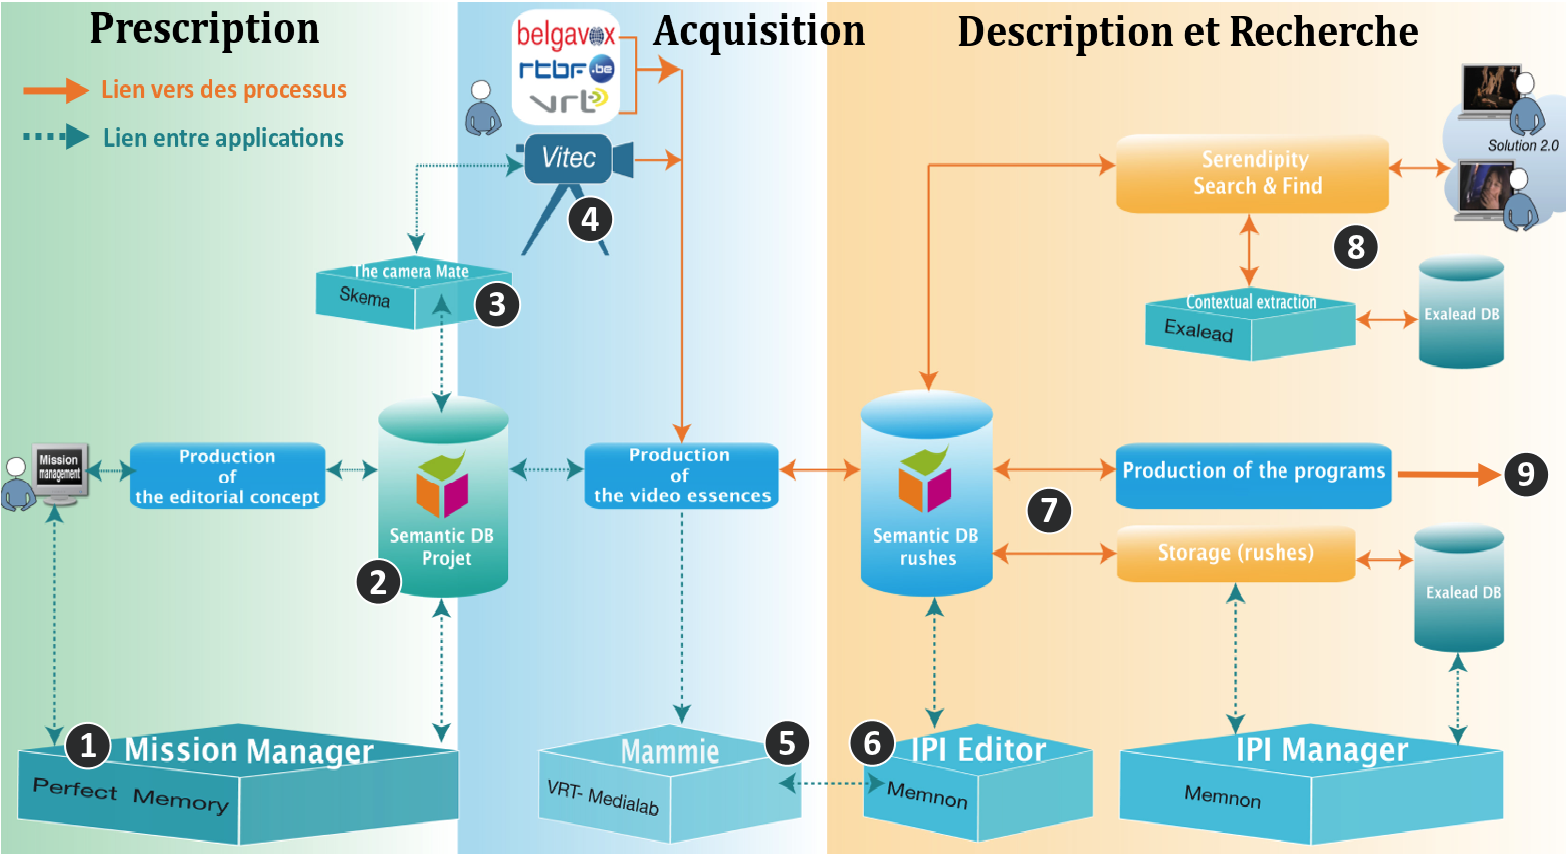
\includegraphics[width=1\textwidth]{./images/Architecture-process-v1.png}
\caption{Architecture finale du projet MediaMap : vue centrée sur le processus}
\label{img:arch-process}
\end{figure}

\begin{listenum}
	\item[(6)] L'acquisition du matériel et des connaissances aboutit à l'intégration de ces éléments à une plate-forme de gestion et de description côté RTBF. 
	La description est enrichi par des méthodes d'analyse automatique du signal ou des ajouts manuels, à différents moments de la post-production.
	Cela permet à l'équipe de post-production de la RTBF de prendre connaissance plus facilement du matériel filmé par ses contributeurs externes. [\g{Enrichissement des descriptions}]
	\co{L'\pc{IPI Editor} développé par Memnon se charge de cette intégration dans une base de stockage du matériel et une base sémantique pour gérer les connaissances qui y sont associées (à l'exception des connaissances sur le processus de production, gérées par le \pc{Mission Manager}.)e
	Parmi les traitements automatiques disponibles sur cette plate-forme, on trouve des analyseurs sonores qui permettent de repérer les moments de musique et de dialogue, et dans ce dernier cas de produire une transcription des paroles synchronisée mot à mot avec le flux audiovisuel.
	Il est également possible de rattacher des connaissances sur le monde au matériel, comme les personnes, les lieux etc.}

	\item[(7)] L'acquisition et la description du matériel audiovisuel peut être ensuite associée avec la structure documentaire du journal télévisé du soir, qui propose également une version Web, mais aussi à l'équipe de production d'un DVD de l'évènement (revoir la section \ref{sec:ex-reuse}, p.\pageref{sec:ex-reuse} pour plus de détails).
	Enfin, certaines séquences seront également mises à disposition à des organisations externes via la base sémantique de description des rush (prises de vue). [\g{Réutilisation}]
	\co{La réutilisation des matériaux audiovisuels dans divers contexte d'exploitation est rendu possible par l'articulation entre la plate-forme de stockage des rush et des bases sémantiques sur le processus de production (\pc{Mission Manager}) et sur les descriptions associées aux documents audiovisuels (\pc{IPI Editor, IPI Manager}), ce qui explique le positionnement de l'étape n°7 sur le diagramme.}

	\item[(8)] Lors du montage du sujet pour le journal télévisé, la RTBF se rend compte qu'ils ont besoin d'un plan de coupe présentant le lieu de représentation de l'évènement culturel, qui n'a pas été commandé aux équipes de tournage. 
	Pour cela, le monteur vérifie d'abord si les équipes de la VRT ou de la RTBF ne l'aurait pas tourné (en plus de la commande), mais aucun plan n'est disponible. 
	De ce fait, une recherche dans la base de rush (prise de vue) est lancée et le monteur récupère un plan existant. [\g{Accès et Recherche}]
	\co{L'interface de gestion du projet du \pc{Mission Manager} permet de visualiser le matériel produit par chaque équipe de tournage, de naviguer dans la structure documentaire du projet.
	La recherche de matériel passe d'abord par une phase d'indexation prise en charge par Exalead et rendu accessible à un interface Web construite par Solution 2.0.
	L'indexation s'effectue par une connexion à l'\pc{IPI Manager} qui gère l'évolution des connaissances sur et associées au document audiovisuel.
	Ces recherches s'effectue avec le même vocabulaire que la définition d'un plan dans un script, et renvoit non seulement à des séquences audiovisuelles, mais également à leur contexte de production (projet, contributeur, structure documentaire etc.). 
	La position de l'étape n°8 sur le diagramme présuppose l'échange d'information entre la base Exalead et la base sémantique de l'IPI Manager.}
	
	\item[(9)] Une fois le sujet pour le journal télévisé produit, la RTBF envoit le projet entier à la VRT, qui le réutilisera en modifiant le commentaire. 
	Ce transfert ne consiste pas simplement à envoyer le montage final, mais l'ensemble des rush, des montages intermédiaires, des commentaires du public flamand, des enrichissement de descriptions etc.
	Il s'agit donc d'un échange de matériel et de connaissances sur ce matériel. [\g{Transport, Échange}]
	\co{Les différentes bases sémantiques peuvent exporter les connaissances stockés afin de les transmettre à d'autres bases, en même temps que l'ontologie qui définit ces connaissances.
	Notre modèle doit également embarquer les variations de vocabulaire utilisé par le recepteur, afin de réaliser l'adaptation de leur expression.}
\end{listenum}



% En faire un tableau
La Table \ref{tab:archaine} clarifie la manière dont le scénario se déroule par rapport à une chaîne de production classique (voir \ref{sec:prod}). 
En effet, notre scénario met en avant de nouvelles pratiques, comme la production collaborative et la réutilisation de fragments dès leur production. 
Nous proposons donc de comparer notre scénario avec les étapes classiques d'un projet de production. 
Alors que la \g{préproduction} est représentée par les phases (1) et (2), les phases (3) et (4) n'existent pas en tant que telles dans un projet de production classique.
En effet, la traduction du script en guide de tournage doit être prise en charge par le contributeur, de même que les caméras ne propose habituellement pas d'assistance pendant le tournage ou de vérification après coup. 
Toutefois, on peut les assimiler à une étape de \g{fabrication} du matériel audiovisuel.
La phase (5) de livraison et (6) d'enrichissement des descriptions correspond à l'étape du \g{dérushing}. 
La phase (7) de réutilisation correspond à plusieurs étapes, puisqu'il s'agit à la fois du \g{montage} et de la \g{finition}. Dans le cas décrit, il s'agit de réutilisation dans le sens où les fragments participent à plusieurs projets de production. 
La phase (8) d'accès et recherche peut être présentée comme une étape \g{archivages} qui serait intégrée à la production. 
La phase (9) de transport et d'échanges peut être mise en rapport avec l'étape de \g{distribution}, quoi que la nature de l'objet échangé varie énormément (des fichiers vidéo ou bien une ensemble de connaissances et de fichiers représentant le projet de production).

\begin{table}
\begin{center}
\begin{tabular*}{0.92\textwidth}{|c|c|c|c|c|c|c|c|c|c|}
\hline
	\multicolumn{2}{|c|}{\g{Pré-production}} & \multicolumn{4}{|c|}{\g{Production}} & \multicolumn{2}{|c|}{\g{Post-production}} & \multicolumn{2}{|c|}{\g{Exploitation}} \\ \hline\hline
	\e{Planning} & \e{Scripting} & \multicolumn{2}{|c|}{\e{Fabrication}} & \multicolumn{2}{|c|}{\e{Derushing}} & \e{Montage} & \e{Finition} & \e{Archivage} & \e{Distribution} \\ \hline
	(1) & (2) & (3) & (4) & (5) & (6) & \multicolumn{2}{|c|}{(7,8)} & (8) & (9) \\ \hline

\end{tabular*}
\caption{Comparaison entre les étapes de le chaîne de production classique (\e{en italique}) et le scénario de production de MediaMap}\label{tab:archaine}
\end{center}
\end{table}


%%%%%%%%%%%%%%%%%%%%%%%%%%%%%%%%%%%%%%%%%%%%%%
%%%%%%%%%%%%%%%%%%%%%%%%%%%%%%%%%%%%%%%%%%%%%%
% \subsection{Architecture du projet MediaMap}\label{sec:arch-compo}
% % Nous présentons les particularités applicatives de l'approche MediaMap

% \begin{figure}[ht!]
% \centering
% 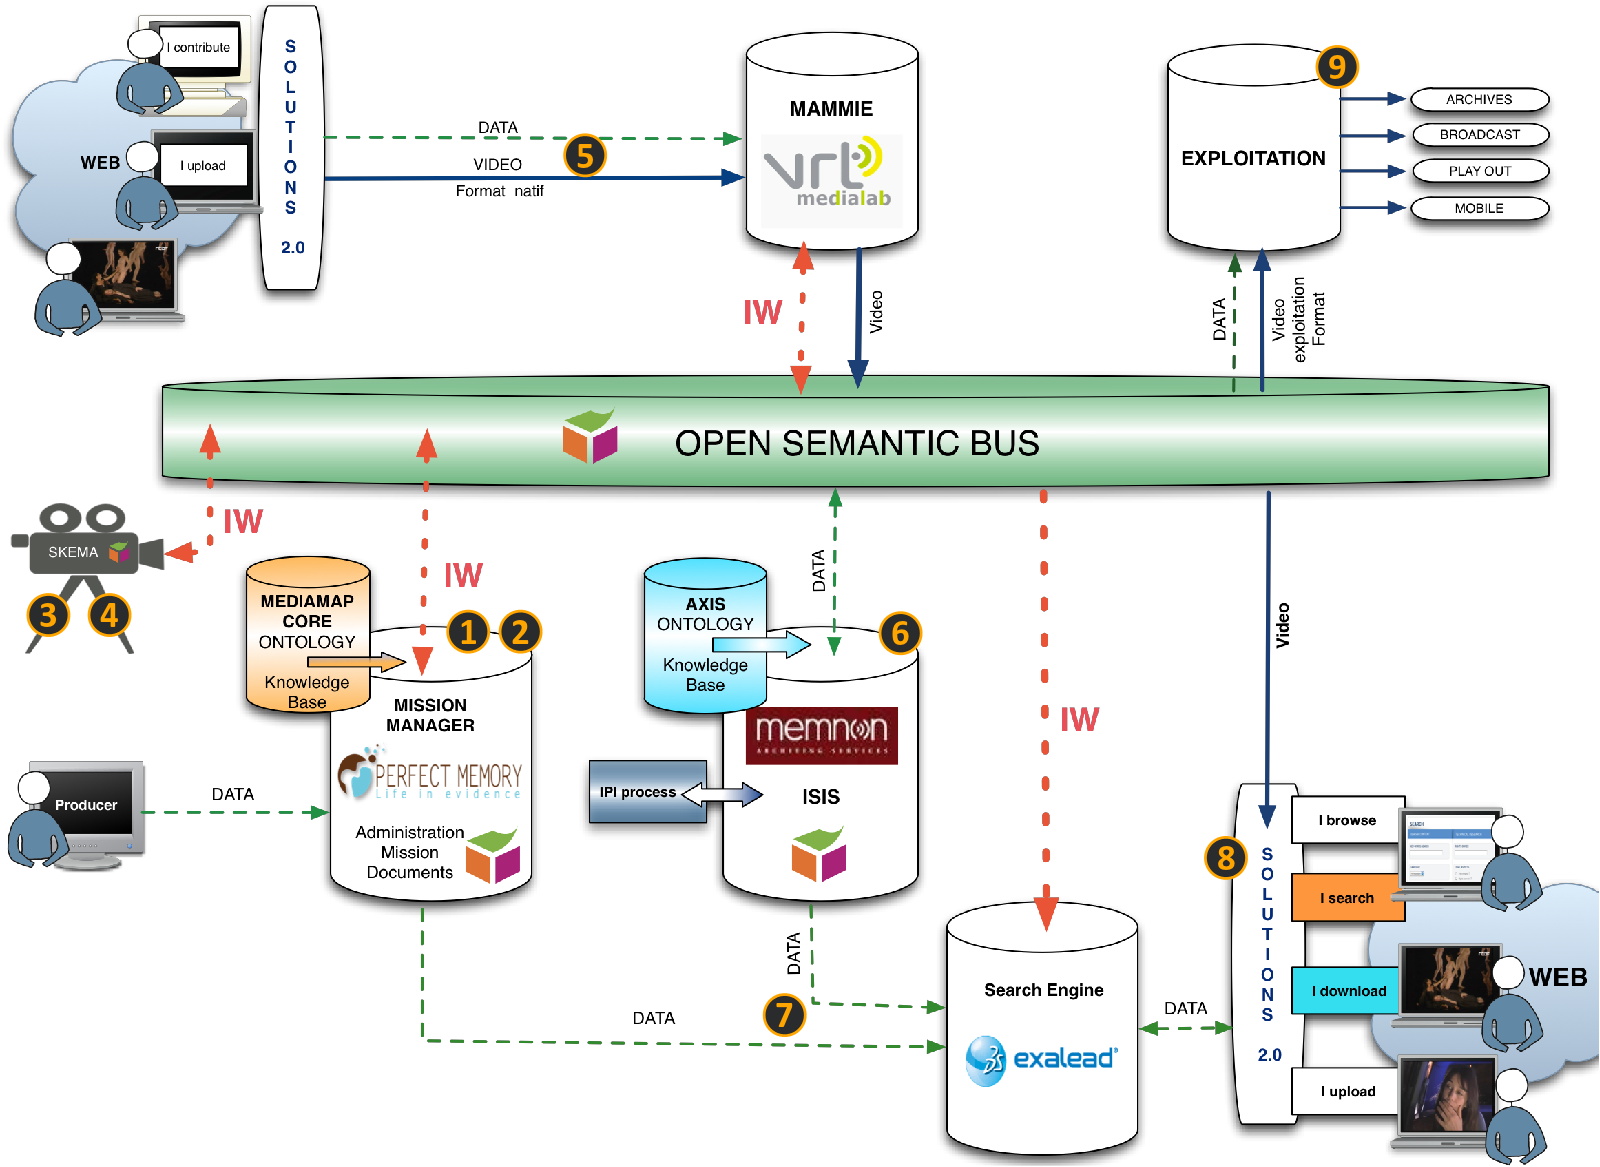
\includegraphics[width=1\textwidth]{./images/Architecture-apps-v1.png}
% \caption{Architecture finale du projet MediaMap : vue applicative des flux de données}
% \label{img:arch-apps}
% \end{figure}


% La Figure \ref{img:arch-apps} reprend la numérotation du scénario et propose une vue alternative centrée sur les flux de données entre les applications. 
% En particulier, l'apparition de l'\pc{Open Semantic Bus} (OSB) et des \pc{Interoperability Wicket} (IW, guichet d'interopérabilité) introduisent des éléments d'une architecture modulaire s'inspirant des architectures distribuées de réseau informatique.
% Un élément caché dans le diagramme est la notion de \pc{Unique Semantic Entity} (USE) qui correspond à un paquet automome de connaissances et qui constitue le format d'échange sur l'OSB.
% En pratique, OSB, IW et USE permettent de réaliser l'interopérabilité des échanges de données et de connaissances entre les applications de la chaîne de production audiovisuelle, regroupant ainsi les fonctions suivantes : 
% \begin{liste}
% 	\item gestion dynamique des applications connectées à l'OSB et des services proposées, à la manière des répertoires de Web Services, de façon à accepter l'ajout ou la suppression de ces derniers.
% 	Cela implique également de décrire les appels et les résultats fournis par ces services.
% 	Il s'agit par exemple de demander une description des formats d'import supportés par une application, d'une description des capacités d'un contributeur, ou bien de ces droits associés à un projet ou une tâche d'un projet.

% 	\item gestion des échanges de données entre applications et entre contributeurs par l'intermédiaire des IW. 
% 	Ces guichets assurent l'acquisition des données et leur comparaison éventuelle avec un attendu.
% 	Ensuite, suivant le destinataire, ils peuvent effectuer des transformations automatiques pour satisfaire aux besoins du récepteur. 
% 	Ces transformations opèrent sur deux niveaux, sur le plan du formatage des données (passage de XML à JSON, ou bien d'un modèle de données à l'autre), et sur le plan de l'expression des connaissances (transformation d'un vocabulaire professionnel en explication pour amateur par exemple).
% \end{liste}

% Parmi les différences avec la Figure précédente, il faut noter la mise en avant des interfaces Web créés par Solution 2.0. 
% Dans le cas de l'étape n°5, la livraison d'un matériel peut alors se faire indépendamment de la caméra "intelligente" et de l'OSB.
% Concernant, l'étape n°8 d'accès et de recherche de matériel, elle peut également être ouverte à des organisations externes.
% Un autre point important sont les différences de nommage. L'\pc{IPI Manager} et l'\pc{IPI Editor} était d'abord nommé ISIS par Memnon, mais ce nom fut changé en fin de projet pour des raisons commerciales. 
% De même, l'\pc{Axis ontology} est en réalité une version modifiée de l'ontologie MediaMap, intégrant des raffinements et des extensions spécifiques à leurs processus d'indexation. 
% Ainsi, l'ontologie construite pendant le projet est utilisée, modifiée et intégrée dans des applications, notamment celles de Memnon et de Perfect Memory.




\subsection{Axes de modélisation}\label{sec:axes}
Comme nous l'avons vu en section \ref{sec:metier}, la production audiovisuelle se présente comme un processus structuré en grandes étapes (pré-production, production, post-production) qui visent la préparation, la fabrication puis l'exploitation d'un document audiovisuel.
S'il existe une diversité de type de production (scriptée, non-scriptée) et de genre de documents (\ref{sec:strat-desc}), celles-ci ne représentent que des variations dans la réalisation des étapes de cette structure générale.  
De la même manière, les pratiques de production collaborative et de réutilisation du matériel existant (\ref{sec:rechaine}) n'entraînent pas de transformation profonde de cette structure, mais plutôt une adaptation de certaines étapes. 
Cependant, l'ouverture de la chaîne à de nouveaux contributeurs ainsi que le focus sur les fragments nécessitent d'affiner la modélisation classique du document audiovisuel et d'en suivre sa construction. 
Ainsi, s'il n'existe pas \e{une} production audiovisuelle, il nous faut modéliser des situations typiques de \e{la} production audiovisuelle, qui pourront s'ajuster aux spécificités \e{des} productions audiovisuelles.

% Notre travail de modélisation se heurte à deux verrous scientifiques, identifiés en section \ref{sec:scien} puis développés dans les chapitre \ref{chap:omod} et \ref{chap:mav}, que nous reformulons en : 
Nous décomposons les problèmes scientifiques que nous avons défini précédemment en deux axes de modélisation principaux. 
L'axe $\alpha$ se rapporte aux situations typiques de la production audiovisuelle (\ref{sec:situations}), alors que l'axe $\beta$ renvoit à des questions de représentation progressive de ces situations, ainsi qu'à la documentation de cette représentation.
Ce dernier axe ne conduit pas à la définition de patrons de conception, mais plutôt à l'enrichissement des patrons existants ainsi qu'à la mise en place de conventions de représentation qui sont distinctes de notre modèle.
Ainsi, leur mise en oeuvre se situe plus au niveau des applications que de l'ontologie que nous avons construites, ce qui nous amène à présenter certaines de ces éléments dans la section \ref{meo}.



\begin{problemes}{LightGoldenrodYellow}
\begin{liste}
 	\item[(\g{$\alpha$})] \g{L'articulation de plusieurs ensembles de connaissances} [\e{$\chi_1$ : autonomie}, \e{$\chi_2$ : réutilisabilité}]. 
 	On distingue ainsi deux ensembles de connaissances : 
 	% à quoi servent-ils ?
 	\begin{listeni} 
 		\item[($\alpha_1$)] L'organisation du \e{processus de production audiovisuelle}, qui décrit la répartition des tâches et  les capacités des \e{contributeurs}.
 		Cet ensemble permet d'associer les connaissances fabriquées par les contributeurs aux documents et de faciliter leur implication et les échanges de connaissances.
 		
 		\item[($\alpha_2$)] L'organisation du \e{document audiovisuel}, c'est-à-dire sa structure documentaire, le \e{matériel audiovisuel} qu'on y attache et une description de leur fabrication (l'\e{écriture filmique} détaillée dans le script).
 		Cet ensemble permet de faciliter la recherche, la gestion et donc la réutilisation des fragments audiovisuels.
 	\end{listeni}

 	\item[(\g{$\beta$})] \g{Une pro(duction/con)sommation progressive et contributive de ces connaissances} [\e{$\delta_1$: multi-jargon}, \e{$\delta_2$ : documentation}, \e{$\delta_3$ : évolution, gestion}].
 	Il s'agit ici du problème de l'évolution et du partage des connaissances liées à un document/fragment audiovisuel tout au long de son ou de ses cycle(s) de vie. 
 	On distingue deux écueils nouveaux suite à l'ouverture de la chaîne à des pratiques de réutilisation : la \e{progressivité de la description}, et la nécesssité de la rendre compréhensible malgré l'\e{hétérogénéité des contributeurs} : 
 	\begin{listeni}
 		\item[($\beta_1$)] \e{Les connaissances sur les document/fragments audiovisuels évoluent et doivent s'ajuster au contexte de production ou de réutilisation}.
 		Les connaissances fabriquées en début de chaîne de production prescrivent un résultat attendu, or de nombeux éléments sont susceptibles d'être modifiés ou précisés par la suite.
 		Il faut donc ajuster les connaissances prescriptives à la réalité des opérations, afin de décrire les résultats effectifs (et non plus l'attendu).
 		Cet écueil apparent est en réalité une opportunité, car la fabrication des descriptions peut alors s'appuyer sur les connaissances prescriptives et les vérifier. 
		De plus, la réutilisation d'un fragment/document audiovisuel dans un nouveau contexte n'implique pas seulement un transfert de matériels audiovisuels, mais également un transfert des connaissances. % mais est-ce que l'on traite vraiment ce cas ? on gère des ensembles de connaissances qui peuvent évoluer (enrichissement)
		Ce transfert peut nécessiter d'extraire certaines connaissances toujours pertinentes et de les associer à celles du nouveau contexte d'utilisation, ou bien de les intégrer à une conceptualisation propre à ce contexte (spécialisation ou bien extension).
		% Cette évolution est rendue possible par 

		\item[($\beta_2$)] \e{Adapter la forme d'expression des connaissances en fonction de l'implication du contributeur dans la chaîne de production et de ses capacités.}
 		Le problème de l'accès aux connaissances est traité par la composition d'une vue contextuelle et spécifique à chaque contributeur de la chaîne, ou chaque groupe de contributeurs.
 		Toute connaissance exprimée à travers le modèle doit pouvoir être caractérisée suivant les codes d'écritures utilisés, eux-mêmes reliées aux capacités des contributeurs.
		Il est alors possible d'effectuer une double sélection ; les connaissances pertinentes suivant l'implication dans la chaîne (en utilisant la description du processus de production); les formes d'expression facilitant leur compréhension (à partir d'une description des capacités des contributeurs).
		% Cette adaptation est rendue possible par le couplage entre conceptualisation, terminologie et documentation.
 	\end{listeni}
\end{liste}
\end{problemes}


Nous pouvons raffiner maintenant ces deux axes de modélisation. 
Voici les situations typiques de la production audiovisuelle que nous avons modélisé en patrons de conception : 
% \begin{problemes}s{LightGoldenrodYellow}
\begin{listeni}
	\item[($\alpha_1$)] l'organisation du \g{processus de production} (\ref{sec:mission}) et du travail de ses \g{contributeurs} (\ref{sec:agent}): 
	\begin{liste}
		\item[($\alpha_1a$)] la division d'un projet de production en sous-tâches et la spécification du résultat attendu ainsi que des moyens fournis pour les remplir .

		\item[($\alpha_1b$)] l'assignation des tâches d'un projet à des contributeurs, ce qui leur confère un rôle, des droits et des responsabilités.
	\end{liste}

	\item[($\alpha_2$)] l'articulation d'un \g{document audiovisuel} et de ses différentes composantes (\ref{sec:opus}), avec leurs descriptions (\ref{sec:annotation}) : 
	\begin{liste}
		\item[($\alpha_2a$)] la gestion des fichiers qui encapsulent le matériel audio-visuel et ces différentes pistes.
		\item[($\alpha_2b$)] la segmentation du matériel audiovisuel.
		\item[($\alpha_2c$)] la structure documentaire qui suit des règles de composition de fragments. 
		\item[($\alpha_2d$)] la description par l'écriture filmique, et ses références à des éléments fictifs ou réels.
	\end{liste}
\end{listeni}
% \end{problemes}


Concernant les aspects concernant la documentation et l'évolution des connaissances : 
\begin{listeni}
\item[($\beta_1$)] Le déroulement de la production a pour conséquence de faire \g{évoluer nos connaissances} sur l'organisation du processus de production et l'articulation du document audiovisuel : 
	\begin{liste}
		\item L'évolution de la description d'un document audiovisuel.
		\item L'échange de connaissances entre organisations.
		\item Les pratiques de réutilisation de fragments documentaires.
	\end{liste}

	\item[($\beta_2$)] L'\g{adaptation des formes d'expressions} aux capacités des contributeurs de la chaîne de production : 
	\begin{liste}
		\item La mise en place d'un thésaurus multi-jargon et d'une documentation des concepts.
		\item L'attribution de compétences linguistiques et professionnelles aux contributeurs (humains, machines).
		\item L'accès personnalisé aux connaissances de la chaîne suivant le contexte (le contributeur, ses capacités, son implication dans la châine).
	\end{liste}
\end{listeni}

\begin{figure}[ht!]
\centering
\includegraphics[width=0.8\textwidth]{./images/Legende-v1.png}
\caption{Légende pour les diagrammes de présentation des patrons de conception}
\label{img:legende}
\end{figure}

Nous avons rappelé les indicatifs de ces axes de modélisation dans les titre des sections suivantes.
Par ailleurs, nous avons utilisé deux types de Figure pour présenter ces patrons (voir Figure \ref{img:legende}) : 
\begin{liste}
	\item les Figures de type \gui{Principaux concepts et relations} permettent de présenter les relations entre concepts pour représenter une situation. 
	Dans certains cas, nous avons ajouté des liens de spécialisation afin de donner directement une vue synoptique sur les possibilités de représentation de ce patron. 
	Les propriétés des concepts sont généralement définis dans le texte.

	\item les Figures de type \gui{Extrait de la structure ontologique} se focalisent sur les liens de spécialisations entre concepts, et permettent de préciser les différences entre concepts frères ainsi que la similarité entre concepts parent-enfants utilisées dans la méthode de construction d'ontologie \pc{Archonte} (\ref{sec:construction}).
	Ces Figures permettent de détailler la formalisation de notre modèle conceptuel. 
	Des exemples d'instanciations seront ensuite présentés dans la section \ref{sec:meo}.
\end{liste}
\input{CONTENU/2-contrib/2a-concepts}
\input{CONTENU/2-contrib/2b-concepts}
\input{CONTENU/2-contrib/3-meo}


% % \cleardoublepage


% %%%%%%%%%%%%%%%%%%%%%%%%%%%%%%%%%%%%%%%%%%%%%%%%%%%%%%%%%%%%%%%%%%%%%%%%%%%%%%%%%%%%%%%%%%%%%%%%%%%
% %%%%%%%%%%%%%%%%%%%%%%%%%%%%%%%%%%%%%%%%%%%%%%%%%%%%%%%%%%%%%%%%%%%%%%%%%%%%%%%%%%%%%%%%%%%%%%%%%%%
\part*{Discussion}
\addcontentsline{toc}{part}{Discussion}
\input{CONTENU/3-disc/1-xps}
\input{CONTENU/3-disc/2-apps}
\input{CONTENU/3-disc/4-validation}

% demande/délégation/assignation d'une tâche, de droits, à un contributeur
% hiérarchie d'activité dans un projet
% fragmentation documentaire 
% segmentation du matériel av
% articulation entre activité et résultat
% description (a priori et a posteriori) d'un fragment documentaire et du matériel audiovisuel
% documentation d'une conceptualisation
% attribution de compétences à un contributeur
% sélection de la documentation suivant les compétences (et/ou) l'implication d'un contributeur dans un projet
% articulation base de faits, documentation, conceptualisation


\chapter*{Conclusion}\label{chap:cc}
\addcontentsline{toc}{chapter}{Conclusion}


\appendix
\part*{Annexes}
\rehead{\headingsf\scshape Annexe~\thechapter}
\noappendicestocpagenum
\addappheadtotoc
\input{CONTENU/3-disc/5-annexes}
% \chapter{}\label{c:}
% \section{}\label{s:}

% \cleardoublepage

%%%%%%%%%%%%%%%%%%%%%%%%%%%%%%%%%%%%%%%%%%%%%%%%%%%%%%%%%%%%%%%%%%%%%%%%%%%%%%%%%%%%%%%%%%%%%%%%%%%
%%%%%%%%%%%%%%%%%%%%%%%%%%%%%%%%%%%%%%%%%%%%%%%%%%%%%%%%%%%%%%%%%%%%%%%%%%%%%%%%%%%%%%%%%%%%%%%%%%%
%%%%%%%%%%%%%%%%%%%%%%%%%%%%%%%%%%%%%%%%%%%%%%%%%%%%%%%%%%%%%%%%%%%%%%%%%%%%%%%%%%%%%%%%%%%%%%%%%%%
%%%%%%%%%%%%%%%%%%%%%%%%%%%%%%%%%%%%%%%%%%%%%%%%%%%%%%%%%%%%%%%%%%%%%%%%%%%%%%%%%%%%%%%%%%%%%%%%%%%
%%%%%%%%%%%%%%%%%%%%%%%%%%%%%%%%%%%%%%%%%%%%%%%%%%%%%%%%%%%%%%%%%%%%%%%%%%%%%%%%%%%%%%%%%%%%%%%%%%%
%%%%%%%%%%%%%%%%%%%%%%%%%%%%%%%%%%%%%%%%%%%%%%%%%%%%%%%%%%%%%%%%%%%%%%%%%%%%%%%%%%%%%%%%%%%%%%%%%%%
%%%%%%%%%%%%%%%%%%%%%%%%%%%%%%%%%%%%%%%%%%%%%%%%%%%%%%%%%%%%%%%%%%%%%%%%%%%%%%%%%%%%%%%%%%%%%%%%%%%
%%%%%%%%%%%%%%%%%%%%%%%%%%%%%%%%%%%%%%%%%%%%%%%%%%%%%%%%%%%%%%%%%%%%%%%%%%%%%%%%%%%%%%%%%%%%%%%%%%%
%%%%%%%%%%%%%%%%%%%%%%%%%%%%%%%%%%%%%%%%%%%%%%%%%%%%%%%%%%%%%%%%%%%%%%%%%%%%%%%%%%%%%%%%%%%%%%%%%%%
%%%%%%%%%%%%%%%%%%%%%%%%%%%%%%%%%%%%%%%%%%%%%%%%%%%%%%%%%%%%%%%%%%%%%%%%%%%%%%%%%%%%%%%%%%%%%%%%%%%
%%%%%%%%%%%%%%%%%%%%%%%%%%%%%%%%%%%%%%%%%%%%%%%%%%%%%%%%%%%%%%%%%%%%%%%%%%%%%%%%%%%%%%%%%%%%%%%%%%%
% \appendix
% \part*{Annexes}
% \rehead{\headingsf\scshape Annexe~\thechapter}
% \noappendicestocpagenum
% \addappheadtotoc

% \cleardoublepage

%%%%%%%%%%%%%%%%%%%%%%%%%%%%%%%%%%%%%%%%%%%%%%%%%%%%%%%%%%%%%%%%%%%%%%%%%%%%%%%%%%%%%%%%%%%%%%%%%%%
%%%%%%%%%%%%%%%%%%%%%%%%%%%%%%%%%%%%%%%%%%%%%%%%%%%%%%%%%%%%%%%%%%%%%%%%%%%%%%%%%%%%%%%%%%%%%%%%%%%
%%%%%%%%%%%%%%%%%%%%%%%%%%%%%%%%%%%%%%%%%%%%%%%%%%%%%%%%%%%%%%%%%%%%%%%%%%%%%%%%%%%%%%%%%%%%%%%%%%%
% \chapter{D'un Web à l'autre : les paradigmes de la lecture informatique}\label{a:webs}
% \KOMAoptions{twoside=no}

\pagestyle{empty}

\input{PERRON/GARDE}

% \newpage

% ~

% \cleardoublepage

% \pagestyle{empty}

% \input{PERRON/REMERCIEMENTS}

% \cleardoublepage

% \KOMAoptions{twoside=yes}

\frontmatter

\pagestyle{scrheadings}

\shorttableofcontents{Sommaire}{2}

\cleardoublepage


%%%%%%%%%%%%%%%%%%%%%%%%%%%%%%%%%%%%%%%%%%%%%%%%%%%%%%%%%%%%%%%%%%%%%%%%%%%%%%%%%%%%%%%%%%%%%%%%%%%
%%%%%%%%%%%%%%%%%%%%%%%%%%%%%%%%%%%%%%%%%%%%%%%%%%%%%%%%%%%%%%%%%%%%%%%%%%%%%%%%%%%%%%%%%%%%%%%%%%%


% \pagestyle{empty}

% ~

% \bigskip

% \vspace{11em}

% \bigskip

% \epigraphii{La totalité est la non vérité.}{Adorno, \ita{Minima Moralia}}

% \cleardoublepage
% \addcontentsline{toc}{part}{État de l'Art}
% \pagestyle{empty}

% ~
% \bigskip

% \vspace{11em}

% \bigskip

% \epigraphii{Se demander si un ordinateur peut penser ... est aussi intéressant que de se demander si un sous-marin peut nager.}{ Edsger Wybe Dijkstra, \ita{The threats to computing science}}

% \pagestyle{scrheadings}

%%%%%%%%%%%%%%%%%%%%%%%%%%%%%%%%%%%%%%%%%%%%%%%%%%%%%%%%%%%%%%%%%%%%%%%%%%%%%%%%%%%%%%%%%%%%%%%%%%%
%%%%%%%%%%%%%%%%%%%%%%%%%%%%%%%%%%%%%%%%%%%%%%%%%%%%%%%%%%%%%%%%%%%%%%%%%%%%%%%%%%%%%%%%%%%%%%%%%%%
\part*{Exposition}
\addcontentsline{toc}{part}{Exposition}

\mainmatter
%%%%%%%%%%%%%%%%%%%%%%%%%%%%%%%%%%%%%%%%%%%%%%%%%%%%%%%%%%%%%%%%%%%%%%%%%%%%%%%%%%%%%%%%%%%%%%%%%%%
%%%%%%%%%%%%%%%%%%%%%%%%%%%%%%%%%%%%%%%%%%%%%%%%%%%%%%%%%%%%%%%%%%%%%%%%%%%%%%%%%%%%%%%%%%%%%%%%%%%
% \section*{Préambule (n)}
% \addcontentsline{toc}{section}{Préambule}



%%%%%%%%%%%%%%%%%%%%%%%%%%%%%%%%%%%%%%%%%%%%%%%%%%%%%%%%%%%%%%%%%%%%%%%%%%%%%%%%%%%%%%%%%%%%%%%%%%%
%%%%%%%%%%%%%%%%%%%%%%%%%%%%%%%%%%%%%%%%%%%%%%%%%%%%%%%%%%%%%%%%%%%%%%%%%%%%%%%%%%%%%%%%%%%%%%%%%%%
\chapter{Introduction}\label{chap:intro}
\minitoc
% \epigraphii{On peut s'étonner que les actes spontanés par lesquels l'homme a mis en forme sa vie, se sédimentent au dehors et y mènent l'existence anonyme des choses. La civilisation à laquelle je participe existe pour moi avec évidence dans les ustensiles qu'elle se donne.}{Merleau-Ponty\\\hfill\ita{Phénoménologie de la perception}}

%%%%%%%%%%%%%%%%%%%%%%%%%%%%%%%%%%%%%%%%%%%%%%%%%%%%%%%%%%%%%%%%%%%%%%%%%%%%%%%%%%%%%%%%%%%%%%%%%%%
% \section{Contexte}\label{chap:contexte}
Le travail de thèse dont nous rendons compte dans ce mémoire s'est déroulé dans le cadre du projet MediaMap\footnote{Voir \url{http://www.mediamapproject.org/}} soutenu par le cluster européen Eureka Celtic et la Direction Générale de la Compétitivité, de l'Industrie et
des Services (DGCIS) du ministère de l'Economie, des finances et de l'industrie.
La participation à ce projet de recherche et développement nous a imprégnés de connaissances sur la production audiovisuelle.
%, les besoins qui émergent des tendances actuelles et les problèmes rencontrés pour les combler. 



%Nous nous intéresserons ensuite (\g{Chapitre \ref{chap:problo}}) aux 


%%%%%%%%%%%%%%%%%%%%%%%%%%%%%%%%%%%%%%%%%%%%%%%%%%%%%%%%%%%%%%%%%%%%%%%%%%%%%%%%%%%%%%%%%%%%%%%%%%%
\section{L'impact du numérique sur l'audiovisuel}\label{sec:motiv}
\e{
La révolution numérique initiée depuis une trentaine d'années en conjonction avec la révolution électronique et informatique, s'est progressivement imposée à tous types d'information et de contenus. 
%jusqu'à devenir prépondérante et indispensable dans un monde informatisé.
Ces mouvements d'informatisation des pratiques et de numérisation de l'information impactent les organisations et les métiers en redistribuant les tâches entre humains et machines. 
Dans le cadre de cette thèse, nous nous pencherons sur le cas de l'audiovisuel et de la numérisation de ce contenu et des informations associées.}

%L'audiovisuel représente à plus d'un titre un objet singulier.
%l'exploitation des contenus numériques est en passe de s'étendre à toutes les étapes du cycle de vie d'un objet audiovisuel. % ? pourquoi exploitation ?
Après une informatisation des étapes de postproduction (logiciels de montage, effets spéciaux etc.) puis des équipements de captation (caméra, micro etc.) et de la distribution du côté des diffuseurs, nous avons connu une véritable explosion d'appareils destinés au grand public (lecteur multimédia portable, appareil photo, téléphone portable, dictaphone etc.).


Plusieurs grands chantiers s'ouvrent désormais dans ce mouvement d'informatisation des étapes de la chaîne de production :
\begin{liste}
	\item L'archivage des contenus de manière à les faire entrer dans l'histoire malgré la dégradation inexorable des supports. 
	Il ne s'agit pas simplement de leur permettre de survivre jusqu'à la prochaine génération d'appareils électroniques, mais également de garantir leur \ciel{lisibilité technique et culturelle}, (\cite[p.~12]{Bachimont2000}).

	\item La préproduction des contenus qui est presque inexistante et qui permettrait de récolter des informations sur les contenus avant même leur fabrication. 
	L'enjeu plus général est d'initier l'indexation des contenus au moment du \e{Scripting} et de la continuer tout au long de la chaîne, chaque étape pouvant rajouter des informations ou bien réévaluer les anciennes.
\end{liste}

À côté de la numérisation et de l'informatisation, il ne faudrait pas oublier le développement considérable des réseaux de télécommunications qui a grandement favorisé les échanges de contenus de manière illégale ou légale, de pairs à pairs (\e{Peer to Peer}), entre diffuseurs et spectateurs (\e{Business to Consumers}) ou entre acteurs professionnels de la chaîne (\e{Business to Business}). 
Ainsi, numérisation et informatisation sont dorénavant implictement associées aux facilités de transfert de ces réseaux. 

Sans tenter de tirer toutes les conséquences de ces révolutions technologiques (électronique et informatisation, numérisation, mise en réseaux) sur les usages des spectateurs et des acteurs de la chaîne de production audiovisuelle, on retiendra trois constats important qui charpentent notre réflexion : 
\begin{liste}
	\item \eg{il existe un nombre croissant de contenus audiovisuels en circulation.}
	L'offre et la demande augmentent de même que les capacités de transfert des réseaux et la généralisation des appareils électroniques de captation et de visionnage.

	\item \eg{les pratiques en lien avec les contenus audiovisuels se développent et s'individualisent.}
	La consommation de ces contenus se joue de plus en plus à un niveau individuel depuis l'apparition d'appareils personnels de communication et de visionnage. 
	De même, la production de contenus est facilité par l'informatisation et les progrès des appareils électroniques de captation. 
	La création de contenus n'est donc plus l'apanage de grandes équipes spécialisées et lourdement équipées.
	
	\item \eg{la numérisation complique le maintien de l'unicité des contenus audiovisuels}. 
	%Le principe même du numérique (\ciel{ça a été manipulé} [Bachimont2010]) repose sur la représentation de l'information et le calcul. 
	L'environnement numérique, par rapport à l'analogique, est plus propice à la copie, le transfert, la fragmentation et la manipulation des contenus ramenés invariablement à une donnée muette quelle que soit sa nature (texte, son, image animée ou non etc.) ou sa signification.
	Ainsi coupé des sens et du sens, les contenus semblent perdre leur identité dans le \gui{monomédia} numérique (\cite[p.~13]{Bachimont2000}) dans lequel on a peine à les gérer pour ce qu'ils représentent. 	

	%plus manipulables au sens où chaque visionnage construit une forme perceptive du contenu 

	%est une reconstruction de leur forme perceptible par des appareils de . Il y a donc par définition une certaine instabilité 
	%mobile, versatile, altérable, mouvant, variable, instable
\end{liste} 

%Le développement de l'électronique a ainsi favorisé une  le nombre de contenus audiovisuels, à favoriser leur circulation
%On constate ainsi une augmentation des sources de contenus ainsi qu'une intensification de leur circulation qui ont des conséquences sur les usages des spectateurs et les acteurs de la chaîne de production.
Nous allons maintenant préciser cet argumentaire et présenter les enjeux posés par la numérisation, l'informatisation et le développement de l'électronique.




%%%%%%%%%%%%%%%%%%%%%%%%%%%%%%%%%%%%%%%%%%%%%%%
\subsection{La numérisation des contenus audiovisuels}\label{sec:num}
Le contenu audiovisuel est avant tout un objet temporel, c'est-à-dire un flux d'images et de sons qui s'écoule en un temps donné. 
Un des enjeux liés à l'audiovisuel constitue alors à trouver une technologie d'enregistrement et de manipulation de ces flux.

\paragraph{L'enregistrement analogique du flux}
Les techniques d'enregistrement analogique reposent sur la conversion continue du flux original en un signal analogue dont les variations s'effectuent sur une échelle physique différente, par exemple une fréquence sonore transformée en une tension électrique. 
L'enregistrement s'effectue sur différents types de supports, cassettes magnétiques, films argentiques etc. 
La caractéristique commune de ces supports est que l'accès au contenu enregistré ne peut se faire que de manière linéaire ou séquentielle, c'est-à-dire qu'il faut avancer ou rembobiner la bande jusqu'au point de départ avant de pouvoir commencer la lecture. 
Ainsi, chaque opération de manipulation de ces contenus compte toujours un temps pas forcément négligeable consacré à l'alignement avec le point de départ désiré. 
Pour bien s'en rendre compte, il suffit de se souvenir du temps qu'il fallait pour rembobiner la cassette de votre film préféré, puis du temps passé en avance rapide pour passer les inévitables publicités précédant le film.

\paragraph{Numérisation et délinéarisation de l'accés}
Avec le numérique, cette expérience autrefois familière a complètement disparu et se voit remplacée par un accès immédiat à n'importe quel moment du contenu audio-visuel. 
La numérisation des contenus consiste à discrétiser le flux en un ensemble de valeurs que l'on convertit ensuite en flux binaire. Ce flux est ensuite enregistré sur des supports de mémoire magnétiques (disquettes 3'1/2, disques durs etc.) optiques (CD, DVD etc.) ou électronique (mémoire vive dite RAM, mémoire flash etc.). 
Seules ces dernières garantissent un accès arbitraire ou délinéarisé aux données stockées en mémoire (n'importe quelle donnée, à n'importe quel moment). 
Les supports magnétiques et optiques proposent un accés séquentiel comme l'analogique, mais plus rapide et surtout que l'on peut coupler avec les mémoires électroniques afin de se rapprocher de leurs performances.

\paragraph{Fragmentation}
Par ailleurs, au-delà des avantages liées aux temps d'accès au contenu, le numérique facilite également sa fragmentation et sa manipulation.
Contrairement à l'analogique, le numérique permet de représenter de manière arbitraire tout type d'information puis d'effectuer des calculs sur ces représentations. 
Ainsi, on peut associer au contenu audiovisuel d'autres contenus de différentes natures pour les enrichir et faciliter son exploitation ultérieure.

\paragraph{Discrétisation}
La discrétisation du flux audiovisuel quant-à-elle remet en cause la temporalité du contenu et permet de ce fait une fragmentation plus aisée et plus fine. 
Lorsque l'analogique effectue une transformation continue et analogue, le numérique définit une fréquence d'échantillonnage et quantifie les valeurs de la source sur une échelle arbitraire finie. 
C'est donc véritablement la fréquence d'échantillonnage qui constitue la première unité de réprésentation de l'information au-dessus du bit.
C'est donc en décidant du nombre de pixels pour représenter une image, ou aux nombres de valeurs par secondes prises pour représenter un son que l'on décide d'une première échelle de fragmentation. 
% Premier niveau de manip technique, ensuite il y a des USI
Toute autre fragmentation à l'échelle supérieure est potentiellement (re)constructible par calcul, pour autant qu'on possède une méthode opérationnalisable. 
%De même que chaque élément de cette fragmentation, chaque unité, devient adressable et donc manipulable par calcul. 
%\cite{Bachimont2000} parle ainsi d'utm, usi ...
% COUPURE DU SENS ?

% \g{== Révision à faire, introduire les UTM et USI ==}
\paragraph{Numériser, c'est informatiser le métier}
Parmi toutes les fragmentations possibles, il convient alors de déterminer leur pertinence par rapport aux types de calculs que l'on souhaite réaliser à chaque étape de la chaîne de production. 
Il s'agit ici de contrôler les calculs à effectuer en suivant les règles du métier qui en disposera.
Chaque étape ayant ses objectifs propres, les calculs effectués varient et s'opèrent à différents niveaux de fragmentation. 
Or la numérisation des contenus et de l'information s'effectue toujours en vue de leur manipulation par des programmes informatiques.
Ainsi, la numérisation entraîne toujours une informatisation qui impacte le métier dans son organisation et ses pratiques parce qu'il transforme les possibilités techniques qui le concerne.
% L'enjeu est donc double, d'une part identifier les niveaux de fragmentation pertinents pour chaque étape de la chaîne de production, et d'autre part de se donner les moyens de reconstruire la cohérence . 

% numériser => (a) fragmenter + (b) mettre en réseau => (a) besoin de conserver la cohérence de l'ensemble + (b) besoin d'autonomiser pour une future situation d'usage





%%%%%%%%%%%%%%%%%%%%%%%%%%%%%%%%%%%%%%%%%%%%%%%
\subsection{Le développement de l'électronique et des réseaux de télécommunications}\label{sec:electro}

L’explosion des appareils multimédia et des possibilités de transférer des contenus par les réseaux de télécommunication a promu de nouvelles pratiques de consommation et d'échanges des contenus tant chez les professionnels de l'audiovisuel que dans le grand public.

Du côté des professionnels, on voit ainsi l’émergence de systèmes de production qui utilisent le réseau pour faire transiter les contenus entre les systèmes d'information de leurs différents départements. 
Ces systèmes reprennent les principes d'architecture multi-tiers utilisés sur le Web avec les contenus représentés par des fichiers ou des flux binaires, d'où leur appelation de \e{file-based production system}.

Ce genre de système favorise également l’échange de fichiers entre organisations, puisque l’architecture permet d'exposer les données stockées de la même manière sur un réseau interne (intranet) ou externe (extranet, Internet).

Du côté du grand public, les appareils portables acquièrent de plus en plus de connectivité avec leur environnement et les réseaux. 
De simples lecteurs à brancher en USB, les appareils sont passés au stade communicant avec la 3G, le Wifi ou le Bluetooth. 
La fonction d'échange se banalise et inversement, les appareils communicant comme les téléphones deviennent eux-même des stations multimédia à part entière, musique, photo, vidéo, courriel, sms etc.\\


Un autre facteur à noter, est que ces appareils portables sont personnels, c’est-à-dire qu’ils sont majoritairement utilisés par un seul individu contrairement à l’usage du téléviseur qui était et reste encore largement un objet collectif. 
Une autre distinction fondamentale se situe dans le fait que ce sont des appareils informatiques qui fonctionnent entièrement dans le numérique. 
Les possibilités d’interaction en font non plus de simples terminaux de lecture, mais potentiellement de véritables instruments de création et de communication. En effet, l'insertion de données et la capture de contenus (photos, sons, textos etc.) est prévu et le couplage avec des plates-formes de publication (réseaux sociaux, dépôts de contenus, CMS etc.) est de mieux en mieux réalisé.

De ce fait, en plus des capacités toujours plus importante de consommation de contenus, ces appareils favorisent eux aussi leur circulation ou la circulation d’information annexes. 
Le partage d’opinions s’est considérablement développé avec la vague d'applications Web dites sociales qui permettaient aux utilisateurs de créer du contenu sans avoir à maîtriser les arcanes techniques du Web. 
Cet ajout d’opinion, même s’il est parfois réduit au minimum à une marque d'appréciation, implique ainsi l’utilisateur dans le processus de diffusion du contenu en le portant à l'attention d'autres utilisateurs (ses contacts dans le cas des réseaux sociaux, ses lecteurs dans le cas d'un weblog ou autres CMS, un ensemble d'utilisateurs anonymes dans le cas de services sociaux tels que Delicious\footnote{Delicious : \url{http://delicious.com/} est une plate-forme de sauvegarde, d'indexation par mot-clé et de partage de marques-pages. Pour l'utilisateur il s'agit soit de sauvegarder et d'indexer ses marques-pages, soit de découvrir les marques-pages correspondant à tel ou tel mot(s)-clé(s) déjà sauvegardées par la communauté. Les grandes tendances d'indexation sont ainsi accessibles à tous, tout en permettant à chacun de développer son système d'indexation personnelle -- adaptation française du mot anglais \e{folksonomy}. Il est également possible de partager directement ses trouvailles avec d'autres utilisateurs par un système d'abonnement et de notification.} ou Digg \footnote{Digg : \url{http://digg.com/} est un site de marque-page social qui fonctione sur le principe du vote. Un utilisateur peut proposer une page qui est alors soumise aux votes des autres utilisateurs. Suivant le succès de la page, celle-ci sera mise en avant sur la page principale de Digg, ou bien mise de côté avec le reste des pages moins populaires, et finira par être supprimée.}).\\


Les appareils numériques multimédia possèdent également des capteurs de plus en plus performant et de moins en moins coûteux qui permettent au grand public de découvrir de nouvelles activités de création (photographie et retouche d’image, tournage et montage vidéo, prise de son et mixage audio etc.).
Cet abaissement du coût d’entrée dans la production a favorisé l'émergence d’une production amateur hétéroclite qui va du passant prenant une photo d’un évènement se déroulant devant ses yeux jusqu’à l’amateur qui pratique par amour mais avec l'exigence d’un professionnel. 
Cette production amateur rentre alors en concurrence avec la production professionnelle, voire la remplace dans certains cas (lorsqu’un passant est le seul témoin d’un évènement inattendu par exemple). 
La concurrence est d'autant plus forte depuis l’apparition de plates-formes de partages qui facilitent la distribution des contenus. 
De manière générale, l’opposition classique entre producteurs et consommateurs se brouille et les professionnels cherchent de plus en plus à mettre à contribution les amateurs dans leurs processus. 
On se dirige ainsi vers un modèle où professionnels et amateurs contribuent à divers degrés et divers moments au cycle de vie des contenus.\\


Avec l'informatisation des appareils multimédia s’est introduit la possibilité de personnaliser la communication avec l'utilisateur, d'y ajouter de l'interactivité et de connecter les utilisateurs entre eux. 
Ces nouvelles possibilités transforment les attendus et les pratiques du grand public. 
De ce fait, cela impacte les rapports avec les professionnels qui tendent à vouloir intégrer les contributions externes à leurs propres productions. 
Ainsi, il ne s’agit plus simplement de produire des contenus qui s'adressent indistinctement aux masses, mais de trouver des moyens de personnaliser son offre, de recommander des contenus, de faciliter la récupération de contenus, de diversifier les occasions de consommer ou de contribuer.








%%%%%%%%%%%%%%%%%%%%%%%%%%%%%%%%%%%%%%%%%%%%%%%
\section{Le projet MediaMap}\label{sec:mm}
% %%%%%%%%%%%%%%%%%%%%%%%%%
\paragraph{Objectifs}
Le projet MediaMap vise à développer des modèles et des applications pour promouvoir la production audiovisuelle collaborative articulant contenus professionnels et amateurs. 
En particulier, l'ambition est d'intégrer les amateurs et leurs contenus dans la chaîne de production professionnelle en améliorant d'une part la qualité technique et éditoriale des contenus fabriqués, et d'autre part en facilitant la collaboration et l'intercompréhension entre les différents acteurs de la chaîne.

La piste de travail retenue a été de construire des ontologies capables de représenter et décrire les contenus au fur et à mesure de leur processus de production. 
Ces informations serviraient de base de connaissances pour de nouvelles applications s'intégrant dès le début à la chaîne de production audiovisuelle, c'est-à-dire dès la conception du contenu. 
Les partenaires du projet ont ainsi développé des applications d'organisation du processus de production, de description du contenu, d'assistance au tournage ainsi qu'un moteur de recherche utilisant ces ontologies comme modèle d'information de référence.

%%%%%%%%%%%%%%%%%%%%%%%%%
\paragraph{Composition}
Le projet MediaMap a rassemblé une dizaine d'entreprises ainsi que deux équipes de recherche de l'Université de Technologie de Compiègne :
\begin{liste}
	\item l'équipe de recherche \pc{Information Connaissance Interaction} (ICI) chargée de la partie modélisation qui a abouti à la construction d'ontologies.

	\item l'équipe de recherche \pc{Automatique, Systèmes Embarqués, Robotique} (ASER) chargée de la conception d 'algorithmes d'analyse d'images et de vidéos.
\end{liste}


Parmi les entreprises du consortium, on compte les deux grandes chaînes de télévision publiques belges ainsi que de nombreuses PME belge ou française qui apportent leurs expertises dans différents domaines :
\begin{liste}
	\item \pc{BelgaVox} qui gère un des plus grands stocks d'archives audiovisuelles belges et produit des documentaires.

	\item \pc{Exalead} qui est un éditeur de solution de recherche pour les entreprises.

	\item \pc{Kane Consulting} qui propose des analyses du marché et des usages aux acteurs de la production audiovisuelle.

	\item \pc{Memnon} qui est spécialisé dans la numérisation, la documentation et l'archivage de contenus audio et vidéo.

	\item \pc{Perfect Memory} qui s'est créé pendant le projet afin d'accompagner les solutions du projet sur le marché grand public et prospecte également le marché professionnel.

	\item \pc{Skema} qui développe des applications de production de contenu audiovisuel amateur pour mobiles et caméras.

	\item \pc{Solution 2.0} qui est une agence de conception et de réalisation de plate-forme Web.

	\item la \pc{Radio-Télévision Belge de la communauté Française} (RTBF).

	\item \pc{Vitec Multimédia} qui développe et manufacture du matériel vidéo numérique.

	\item la \pc{Vlaamse Radio- en Televisieomroep} (VRT).
\end{liste}









%%%%%%%%%%%%%%%%%%%%%%%%%%%%%%%%%%%%%%%%%%%%%%%
\section*{Organisation du mémoire}\label{sec:plan}
\addcontentsline{toc}{section}{Organisation du mémoire}

\paragraph{Exposition}
\e{
La première partie de ce mémoire a pour objectif de présenter les problèmes qui se posent à la production audiovisuelle depuis son avancée vers la numérisation. 
Elle nous permet également de préciser la manière dont nous posons le problème, à la fois en terme métiers et avec nos lunettes de scientifiques.}

Le chapitre \g{\ref{chap:intro}. Introduction} nous sert à rappeler le contexte technologique général qui s'impose au monde de l'audiovisuel. 
En effet, la production audiovisuelle se dirige progressivement vers une numérisation et une mise en réseau de ses produits ainsi qu'une informatisation de ses pratiques qui n'est pas sans conséquences. 

Le chapitre \g{\ref{chap:problo}. Problématisation} nous permet de préciser comment ces tendances impactent le monde de l'audiovisuel.
Nous nous appuyerons sur l'étude du fonctionnement de la chaîne de production audiovisuelle classique (\ref{sec:prod}) pour dresser un bilan des attentes des professionnels vis-à-vis du numérique (\ref{sec:besoins}).
% En particulier, 
Nous précisons alors la manière dont nous posons le problème sur le plan métier, ce qui nous amènera à définir le problème scientifique. 
Sur le plan métier, le défi posé par le numérique consiste à passer d'une vision à l'échelle du document à une vision à l'échelle du fragment. 
En effet, le numérique favorise la fragmentation et la circulation des contenus qu'il s'agit alors de rendre autonome pour en permettre l'exploitation (\ref{sec:pmetiers}). 
Sur le plan scientifique, nous posons le problème en terme de modélisation des objets audiovisuels et des connaissances associées afin de construire une compréhension commune et dynamique pour tous les acteurs impliqués dans la production audiovisuelle (\ref{sec:scien}).
% Nous concluons en expliquant comment nous mobilisons diverses disciplines scientifiques pour construire une réponse aux problèmes posés (\ref{sec:posd}).
% proposent d'une part des outils et des méthodes de modélisation, et d'autre part proposent des modélisations de l'audiovisuel (\ref{sec:posd}).


\paragraph{État de l'art}
\e{
La deuxième partie de ce mémoire vise à étudier des outils, méthodes et langages de modélisation. Elle permet également d'étudier les modélisations existantes des objets audiovisuels, mais égalements des connaissances métiers qui y sont associées afin de faciliter leur exploitation.}

Le chapitre \g{\ref{chap:omod}. Outils de modélisation} commence par clarifier les besoins de modélisations à partir d'un scénario de production collaborative impliquant des acteurs professionnels et amateurs (\ref{sec:cdcf}).
Ces besoins ne se situent pas seulement au niveau de la modélisation conceptuelle, mais également sur le plan des jargons utilisées pour présenter ces concepts à des contributeurs de la production.
Ainsi, nous examinons les définitions des concepts de \gui{systèmes d'organisation de connaissances} (SOC) et en particulier les relations qu'entretiennent \gui{terminologie} et d'\gui{ontologie} (\ref{sec:defs}).
Nous étudions ensuite les langages de structuration et de représentation des connaissances qui permettent de modéliser ces deux types de SOC (\ref{sec:mods}).

Le chapitre \g{\ref{chap:mav}. Modélisations de l'audiovisuel} a pour objectif de mettre en rapport les représentations des professionnels de la production avec diverses communautés scientifiques, en vue de clarifier la définition d'un objet audiovisuel (\ref{sec:dav}) et de sa réutilisation (\ref{sec:gest}).
Cette étude s'appuie sur la poursuite du scénario d'usage du chapitre précédent, et met en exergue la nécessité de fragmenter la modélisation des objets audiovisuels pour favoriser leur réutilisation (\ref{sec:cdc-av}).
Nous étudions ensuite les solutions utilisées dans l'industrie pour gérer la circulation des programmes (\ref{sec:wrapper}) et les décrire (\ref{sec:desc}).
Cette dernière partie analyse les méthodes de fabrication de ces description ainsi que leur nature, puis les modélisations développées.
Une attention particulière est portée à de MPEG-7 (\ref{sec:mpeg7}), qui tient lieu de référence à de nombreux travaux de formalisation sous la forme d'ontologie (\ref{sec:mpeg7etc}).
Nous présentons également des approches de description plus proche de la perspective de la production audiovisuelle (\ref{sec:plan}).


\paragraph{Contribution}
\e{La troisième partie de ce mémoire présente notre contribution conceptuelle et informatique aux problèmes de modélisations que nous avons soulevées.
Nous détaillons nos choix de représentation pour opérationnaliser notre contribution en une ontologie informatique.}

Le chapitre \g{\ref{chap:mod}. Approche et modélisation} revient sur les langages et les modélisations étudiés dans le chapitre précédent et introduit les principes de notre approche (\ref{sec:principes}).
Notre positionnement au sein de la chaîne de production audiovisuelle, nous permet de modéliser le déroulement de la chaîne, la définition d'une structure documentaire première, puis les fragments audiovisuels construits ainsi que les connaissances qui s'y rapportent.
Nous détaillons la modélisation conceptuelle en parties, chacune correspondant à un besoin fonctionnel, en expliquant leur mise en relation par des exemples (\ref{sec:concept}).

Le chapitre \g{\ref{chap:op}. Mise en oeuvre} présente la représentation informatique de notre conceptualisation.
Nous argumentons d'abord nos choix de langage et montrons comment nous les utilisons (\ref{sec:ln}). 
Nous détaillons ensuite la structuration de notre ontologie et son articulation avec des thésaurus et des bases de faits (\ref{sec:op}).

\paragraph{Discussion}
\e{La dernière partie de ce mémoire montre comment notre contribution est utilisé dans le cadre du projet MediaMap et ouvre la discussion sur ce travail de thèse.}

Le chapitre \g{\ref{chap:app}. Applications et expérimentations} introduit les diverses applications qui ont été développé (\ref{sec:app}) par nos partenaires et les expérimentations qu'elles ont permis de mener (\ref{sec:xp}).
Il s'agit d'éclairer l'appropriation de notre travail dans le cadre de scénarios de production audiovisuelle collaborative.
En particulier, nous expliquons quelle partie de l'ontologie est mobilisée par les applications pour construire ou bien intégrer des connaissances sur la production, ses contributeurs et ses produits.

La \g{Conclusion} remet en perspective notre contribution et les applications développées par rapport aux problèmes métiers et scientifiques posés.
Nous ouvrons également la discussion sur la poursuite de nos recherches et l'avenir des applications du projet MediaMap.

\chapter{Problématisation}\label{chap:problo}
\minitoc
\section{La production audiovisuelle}\label{sec:metier}
% faire le point sur ce que le numérique pourrait apporté à la production audiovisuelle
\e{
L'objectif de cette première section est de donner des éléments de compréhension du métier de la production audiovisuelle.
Dans un premier temps, nous rappelons comment s'organise classiquement la fabrication des objets audiovisuels (\ref{sec:prod}).
Ensuite, nous détaillons les notions et des mots utilisées par les professionnels pour parler de l'objet audiovisuel à construire (\ref{sec:docvoc}).
Enfin, à partir de ces éléments nous précisons les besoins que rencontrent ces professionnels avec l'émergence du numérique et de la mise en réseau (\ref{sec:besoins}). 
}


%%%%%%%%%%%%%%%%%%%%%%%%%%%%%%%%%%%%%%%%%%%%%%%
\subsection{Déroulement de la chaîne de production}\label{sec:prod}
% \addcontentsline{toc}{subsection}{La production audiovisuelle}
La création de documents audiovisuels est une entreprise collective qui suit généralement ce qu'on appelle la chaîne de production audiovisuelle. 
Organisée de manière linéaire, cette chaîne peut se décomposer en 4 grandes étapes -- voir Figure \ref{img:intro:chaine}.

\begin{liste} 
	\item \g{Préproduction} : Cette première étape consiste à construire une ébauche du futur document audiovisuel de manière à prévoir les moyens à engager pour le réaliser.

	\item \g{Production} : Cette étape vise à tourner plusieurs prises pour chaque partie du document et à commencer à faire le tri entre elles.

	\item \g{Postproduction} : L'objectif est d'assembler les prises et de les retoucher de manière à former un document cohérent et adapté à une audience et un mode de distribution.

	\item \g{Exploitation} : Une fois le document achevé, on valorise sa construction par une distribution auprès d'une audience ainsi qu'un archivage qui permettra de le réutiliser ultérieurement.
\end{liste}

\begin{figure}[ht!]
\centering
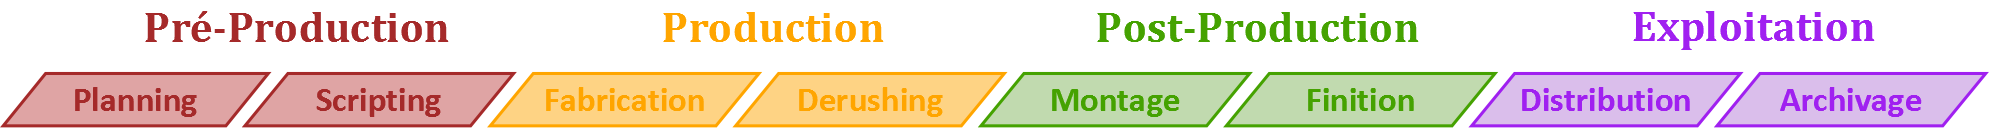
\includegraphics[width=\textwidth]{images/Workflow-Thesis-v0.png}
\caption{La chaîne de production audiovisuelle classique}
\label{img:intro:chaine}
\end{figure}


%%%%%%%%%%%%%%%%%%%%%%%%%
\subsubsection*{Préproduction}\label{sec:preprod}
L'objectif de cette étape est de construire une ébauche du futur document audiovisuel, de manière à prévoir les moyens à engager pour le réaliser. 
On distingue deux phases de préparation, l'écriture ou \e{Scripting} et le \e{Planning} ou planification.

À partir d'une idée, l'écriture du document se déroule en plusieurs étapes où l'on fixe progressivement le message à faire passer ainsi que sa forme audiovisuelle. 
Une fiction par exemple s'écrit à partir d'un résumé de l'histoire, puis on développe les scènes, les personnages, les lieux, les dialogues, etc. jusqu'à arriver à la manière dont cette histoire sera racontée à l'écran. 
On fixe ainsi le type de plan à filmer, les mouvements de caméra, le type de lumière, etc. 
Dans certaines grosses productions, on aura même recours au dessin pour aider à la représentation visuelle.


Toutes ces informations sur le contenu et la forme du futur document audiovisuel servent à estimer le temps nécessaire et les moyens à engager. 
L'estimation du coût d'une production est un élément essentiel pour la production audiovisuelle. 
En effet, dès le départ le producteur doit estimer la rentabilité du futur document afin de voir quels moyens il peut engager. 
Il s'agit bel et bien d'investissement, parfois très lourd, surtout en comparaison avec d'autres industries culturelles – musique, littérature, radio, presse – à l'exception récente du jeu vidéo. 
Contrainte budgétaire et forme esthétique sont donc en négociation dans cette première étape.


%%%%%%%%%%%%%%%%%%%%%%%%%
\subsubsection*{Production}
Une fois l'ébauche et les moyens déterminés, la production vise à réaliser chaque partie du document une à une puis à les assembler en un montage cohérent.

La phase de \e{Fabrication} consiste à capter du réel que l'on a mis en scène. La captation d'un évènement est réalisée grâce à des appareils d'enregistrement (caméra, microphones, etc.). 
La mise en scène du réel se construit à partir d'un ensemble de techniques, d'équipements et d'accessoires (lumière, costume, décors, maquillage, etc.) qui permettent d'obtenir l'image et le son souhaités. 
La technique est ainsi mobilisée dans un objectif esthétique. 
Dans le cas d'une fiction, la fabrication du contenu se fait en fonction du planning de mobilisation des personnes et des équipements plutôt que suivant l'ordre chronologique de l'histoire. 
On regroupe ainsi le tournage des scènes dans tel lieu ou avec tel équipement afin de réduire les coûts. Au final, la fabrication
produit des séquences vidéo et audio qu'il s'agit ensuite de redécouper pour mieux les assembler.

La phase de \e{Derushing} consiste à examiner les séquences réalisées pendant la fabrication et à les trier en vue de faciliter le montage. 
Par exemple, le tournage d'une fiction produit des séquences vidéo comprenant plusieurs prises d'une même scène et souvent des séquences captées par des caméras ayant des angles de prise de vue différents. 
Il faut donc redécouper les séquences en prises puis regrouper les prises d'une même scène. 
Le montage se fera d'autant plus facilement qu'on saura également identifier la qualité et les avantages de chaque prise d'une même scène.


%%%%%%%%%%%%%%%%%%%%%%%%%
\subsubsection*{Postproduction}
Lorsque le contenu audiovisuel est fabriqué et trié, il reste à le structurer en un document et à le conditionner en fonction de sa future exploitation.

La phase de \e{Montage} consiste à agencer des petites séquences de vidéo et d'audio pour construire la structure du document audiovisuel.
L'agencement des plans, leur durée et la transition entre ces plans constituent les ressorts esthétiques propres à l'audiovisuel. 
Ils participent à la transmission du message en ceci qu'ils servent de raccord entre les plans, comme le souligne le réalisateur \pc{Sergueï Mikhaïlovitch Eisenstein}\footnote{L'origine de cette fameuse citation est assez obscur, on la retrouve dans de nombreux documents, dont cet article --\cite{Montage et Réalisme}-- datant des années 60 et extrait de la revue québecoise \gui{Séquence : La revue du cinéma}.} :

\begin{cico}
Le montage est l 'art d'exprimer ou de signifier par le rapport de deux plans juxtaposés de telle sorte que cette juxtaposition fasse naître l'idée ou exprime quelque chose qui n'est contenu dans aucun des deux plans pris séparément. L'ensemble est supérieur à la somme des parties.
\end{cico}

Après le montage, une phase de \e{Finition} est nécessaire pour intégrer d'autres ressources au document en fonction de sa distribution. 
Pour une diffusion antenne d'un reportage, on ajoute le logo de la chaîne de télévision, un jingle, le nom des intervenants ou des titres, etc. 
Une diffusion sur DVD nécessitera l'ajout des conditions
légales d'usages, l'intégration d'un menu de navigation, etc. 
La distribution détermine également un format d'encapsulation (.avi, .mkv, .ogg etc.) et un encodage du contenu audiovisuel (MPEG-2, H.264, MPEG-4, theora vorbis etc.). 
Le résultat de cette phase de post-production est de fournir des documents prêts à l'usage et dans certains cas plusieurs variantes pour chacun des modes de distribution envisagés.


%%%%%%%%%%%%%%%%%%%%%%%%%
\subsubsection*{Exploitation}
Une fois le document achevé, on valorise sa construction par une distribution auprès d'une audience ainsi qu'un archivage qui permettra de le réutiliser ultérieurement.

La phase de \e{Distribution} consiste à rendre le document matériellement accessible à une audience. 
Il s'agit d'un transfert qui peut faire l'objet d'une transaction commerciale ou s'appuyer sur d'autres types de modèles économiques (publicité entre autres). 
La nature du transfert varie et porte à la fois sur les modalités d'accès au contenu et les droits d'usages.

La phase d'\e{Archivage} consiste le plus souvent à stocker le contenu diffusé afin de pouvoir le réutiliser tel quel plus tard, soit en le rediffusant, soit en le vendant à un autre diffuseur. 
C'est aussi généralement la phase où l'on construit, récupère et attache des descriptions du contenu au document audiovisuel. 
En effet, l'archivage n'a de sens que s'il permet de retrouver, voire redécouvrir, les documents archivés.
\ciel{Au plan économique, un film est un bien informationnel, d'expérience, caractérisé par une très forte densité d'informations. Son exploitation s'organise autour de versions différentes, distribuées sur des marchés distincts par des acteurs spécialisés.} (\cite{Blanc2006}).%Gilles Le Blanc - Innovations numériques, distribution et différenciation  : le cas de la projection numérique dans le cinéma.




%<TODO
%TODO>
\subsection{Documents et vocabulaire de la production}\label{sec:docvoc}
\e{
Dans cette section, nous présentons des définitions utilisées dans le milieu professionnel et tirées du \gui{Dictionnaire technique du Cinéma (\cite{Pinel2008})} afin de présenter les principaux documents et le vocabulaire utilisé pendant la phase de préproduction. 
Il s'agit ainsi de mettre en exergue la manière dont se construit une description textuelle de l'objet audiovisuel en devenir ainsi que le vocabulaire utilisé pour faire cette description.}
% Des éléments qui nous serviront à mieux cerner les problèmes qui se posent à la production audiovisuelle.

\paragraph{La notion de plan}
La notion de plan peut se présenter de diverses manières suivant le point de vue adopté. 
Du point de vue technique, il s'agit d'une série d'images (ou photogrammes) qui sont enregistré par un appareil de capatation (une caméra) au cours d'une même prise de vue : \ciel{série de photogrammes enregistrés au cours d'une même prise} (\cite{Pinel2008}).
Il s'agit donc de l'enregistrement qui est effectué entre le moment où l'on presse sur le bouton pour lancer et celui où l'on arrête l'enregistrement.
Cette définition, certes robuste, ne permet pas pour autant de caractériser les plans ou de les comparer entre eux. 
Ainsi, on s'intéresse au point de vue de l'écriture filmique et de la réalisation qui considère non seulement l'action d'enregistrement, mais également la manière dont il est effectué : 

\ciel{
Fragment de temps et d'espace enregistré d'un seul tenant, selon un point de vue déterminé, et donnant à la projection le sentiment de la continuité d'une même \e{image en mouvement}.} (\cite{Pinel2008})

Cette définition complète la précédente en considérant le rapport au sujet (le point de vue) et la temporalité du plan et son rapport à un ensemble d'autres plans (la continuité). 
Elle permet d'envisager les plans comme des éléments de base que l'on assemblera ensuite pour construire un objet audiovisuel : 

\ciel{
La notion de plan est apparue [\dots] lorsqu'on a abandonné le point de vue unique du tableau pour envisager le sujet sous différents angles et à différentes distances et lorsque, par la grâce du montage, on a mis en relation ces plans entre eux.
[\dots]
Si le photogramme représente l'unité technique de la prise de vues, la scène et la séquence les unités narratives de l'oeuvre cinématographique, le plan est la cellule fondamentale de l'écriture du film, de sa préparation jusqu'à la copie standard.} (\cite{Pinel2008})

Dans cette citation, on voit aussi émerger l'idée qu'il existe différents niveaux d'analyse dans l'objet audiovisuel : 
\begin{liste}
	\item un \g{niveau technique} avec le photogramme mais également le pixel dans le numérique.
	\item un \g{niveau narratif} avec la scène (unité de temps et de lieu dans l'histoire) et la séquence (suite de scènes constituant une action dramatique autonome ou distincte).
	\item \g{un niveau dont le plan est l'unité de base qui sert tout au long de la chaîne de production}. 
	On parle d'unité, car il s'agit du résultat de base d'une prise de vue, c'est-à-dire de la fabrication (production) de l'objet audiovisuel. 
	La pré-production, étape de préparation du tournage, utilise donc naturellement cette unité. 
	De même, le montage consiste à organiser ces plans pour former un ensemble cohérent, quitte à les ajuster (raccourcir, allonger, modification du cadrage etc.). 
	Ainsi, il semble que cette unité servent non seulement d'unité de travail de référence pour la chaîne de production\footnote{La production sonore d'un objet audiovisuel ne s'organise pas forcément de la même manière que celle de la production de l'image. Néanmoins, par la force des choses, la construction de l'image prime bien souvent sur celle du son et son unité de base sert donc de référence même pour la production sonore.}, mais également du premier niveau signifiant propre à l'audiovisuel (l'image seul pouvant être rattaché à la photographie).
\end{liste}

Ces distinctions nous permettent de définir le plan selon les caractéristiques suivantes : 
\begin{liste}
	\item \g{l'échelle relative du cadre par rapport au(x) sujet(s)} (personnages, objets etc.).
	C'est ce qui permet de définir un ensemble de \gui{valeurs de plan}, gros plan, plan américain etc. que nous définirons par la suite.
	
	\item \g{l'angle de la prise de vue} (plongée, contre-plongée, cadre incliné etc.)

	\item \g{le mouvement de la caméra} et d'autres paramètres de son objectif (panoramique, travelling, rotation, zoom, focale, focus etc.)

	\item \g{l'articulation des plans entre eux}, d'une part en terme de durée, mais aussi en terme de transition et d'impression de continuité entre les plans. 
	Par exemple, il existe des règles de cadrage et de montage pour aider les spectateurs à situer les personnes sur un plateau\footnote{La règle des 180° oblige ainsi à maintenir les mêmes relations est-à-gauche/droite-de entre les personnes, de manière à ce que le spectateur puisse se souvenir des positions des interlocuteurs sur un plateau. En inversant ces relations topographiques, on donne l'impression au spectateurs que les personnes ont échangé leurs places alors que c'est juste la caméra qui a changé de point de vue. Il s'agit donc d'une règle très importante pour assurer la continuité et la compréhension du spectateur.}.
\end{liste}


\paragraph{Valeurs de plan utilisées dans un script}
La valeur de plan est un des éléments le plus utilisé pour distinguer les plans entre eux, notamment au moment de l'écriture. 
Plutôt que de préciser les paramètres optiques de la caméra (considérés comme des détails très difficile à préciser à l'avance), le réalisateur préfère parler d'un type de plan pour donner une idée générale de l'image à obtenir. 
Le Tableau \ref{tab:vplans} présente les principales valeurs de plans utilisées par les professionnels, avec leur abréviations et leur(s) dénomination(s) anglaise(s) tandis que la Figure \ref{img:intro:plans} en propose une illustration.

\begin{table}[ht!]
   \begin{center}
		\begin{tabularx}{\textwidth}{|p{100pt}|X|p{100pt}|}
		   \hline
	\pc{Dénomination française} & \pc{Défintion} & \pc{Dénomination anglaise} \\ \hline\hline
 	\g{très gros plan (t.g.p.)} & plan cadrant une partie du visage, un détail du corps (un oeil, une bouche, un doigt etc.) ou le détail d'un objet. & extreme close-up, e.c.u. ; big close-up, b.c.u.\\ \hline

 	\g{gros plan (g.p.)} & plan isolant un visage, généralement cadré à la hauteur du noeud de cravate, ou un autre détail du corps (plan de détail ; insert), voire \e{tout ou partie d'un petit objet}. & close-up, c.u.\\ \hline

	\g{plan rapproché} & plan cadrant le(s) personnage(s) au niveau de la taille (plan rapproché taille, p.r.t.) ou de la poitrine (plan rapproché poitrine, p.r.p.). & medium close-up, m.c.u.\\ \hline
	
	\g{plan ceinture} & plan coupant les personnages au niveau de la ceinture & belt shot\\ \hline 

	\g{plan américain} (p.a.) & plan coupant les personnages à mi-cuisse & american shot ; medium close-shot, m.c.s.\\ \hline
	
	\g{plan moyen (p.m.) ou plan en pied} & plan présentant le(s) personnage(s) en pied. Il existe également des variations de ce plan qui sont nommées \e{serré} (aussi nommé plan américain large) ou \e{large} et qui font varier légèrement le cadrage. & medium shot, middle-shot, mid-shot, m.s. ; full shot, f.s.\\ \hline
	

	\g{plan de demi-ensemble (p.d.e., 1/2e.)} & plan mettant en place les personnages dans leur milieu en cadrant une bonne partie du décor & medium-long shot, m.l.s.\\ \hline

	\g{plan d'ensemble (p.e.)} & plan cadrant l'ensemble du décor construit & long shot, l.s.\\ \hline
	
	\g{plan de grand ensemble (p.g.e.)} & plan cadrant l'ensemble du décor construit de grande envergure. & very long shot, v.l.s.\\ \hline

	\g{plan général (p.g.)} & plan couvrant un vaste ensemble qui situe le décor construit dans son cadre : le décor dans le décor. & master shot ; extreme long shot, e.l.s\\ \hline 
		\end{tabularx}
		\caption{Valeurs de plans : du plus précis au plus général \label{tab:vplans}}
   \end{center}
\end{table}

% \begin{liste}
% 	\item \g{très gros plan} (t.g.p.) : \ciel{plan cadrant une partie du visage, un détail du corps (un oeil, une bouche, un doigt etc.) ou le détail d'un objet}. [extreme close-up, e.c.u. ; big close-up, b.c.u.]

% 	\item \g{gros plan} (g.p.) : \ciel{plan isolant un visage, généralement cadré à la hauteur du noeud de cravate, ou un autre détail du corps} (plan de détail ; insert), voire \ciel{tout ou partie d'un petit objet}. [close-up, c.u.]

% 	\item \g{plan rapproché} : \ciel{plan cadrant le(s) personnage(s) au niveau de la taille (plan rapproché taille, p.r.t.) ou de la poitrine (plan rapproché poitrine, p.r.p.).} [medium close-up, m.c.u.]
	
% 	\item \g{plan ceinture} : plan coupant les personnages au niveau de la ceinture [belt shot] 

% 	\item \g{plan américain} (p.a.) : \ciel{plan coupant les personnages à mi-cuisse} [american shot ; medium close-shot, m.c.s.]
	
% 	\item \g{plan moyen} (p.m.) ou \g{plan en pied} : \ciel{plan présentant le(s) personnage(s) en pied.} [medium shot, middle-shot, mid-shot, m.s. ; full shot, f.s.]
% 	Il existe également des variations de ce plan qui sont nommées \ciel{serré} (aussi nommé plan américain large) ou \ciel{large} et qui font varier légèrement le cadrage.

% 	\item \g{plan de demi-ensemble} (p.d.e., 1/2e.): \ciel{plan mettant en place les personnages dans leur milieu en cadrant une bonne partie du décor}. [medium-long shot, m.l.s.]

% 	\item \g{plan d'ensemble} (p.e.) : \ciel{plan cadrant l'ensemble du décor construit}. [long shot, l.s.]
	
% 	\item \g{plan de grand ensemble} (p.g.e.) : \ciel{plan cadrant l'ensemble du décor construit de grande envergure}. [very long shot, v.l.s.]

% 	\item \g{plan général} (p.g.) : \ciel{plan couvrant un vaste ensemble qui situe le décor construit dans son cadre : le décor dans le décor}. [master shot ; extreme long shot, e.l.s] 
% \end{liste}
%TODO:source

\begin{figure}[ht!]
\centering
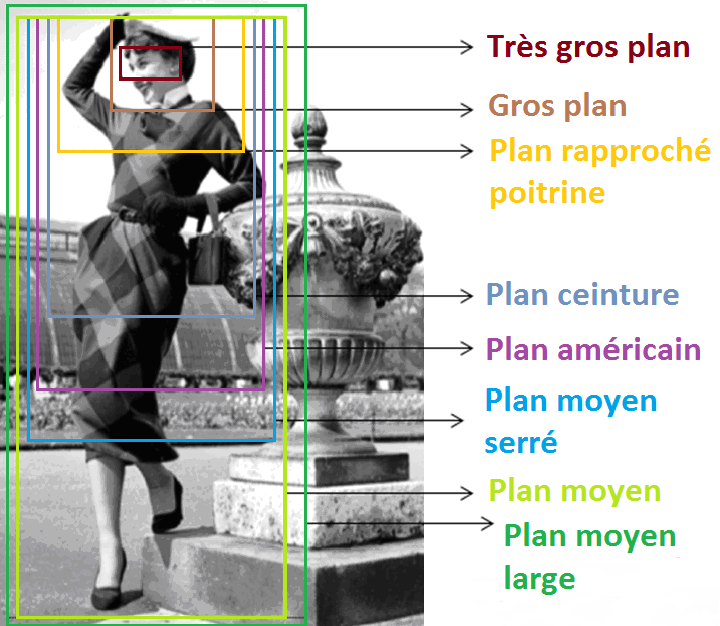
\includegraphics[width=0.4\textwidth]{./images/ValeurPlan-v1.png}
\caption{Différentes valeurs de plan pour le cadrage d'un personnage à l'écran}
\label{img:intro:plans}
\end{figure}


\paragraph{Quelques documents de (pré)production}
%TODO:description + source
La pré-production se repose sur différents types de documents qui permettent de faire émerger progressivement la structure narrative ou documentaire, le découpage en plans et tous les détails de réalisation nécessaire à une bonne préparation du tournage. 
On notera que chacun de ces documents constitue un jalon dans la préparation du projet et que le script, résultat final de cette écriture, constitue une sorte de cahier des charges de l'objet audiovisuel à fabriquer.
\begin{liste}
	\item \g{sujet} : \ciel{matière première du film enrichie et développée lors de la préparation puis mise en forme au cours de la réalisation et du montage.} 
	
	\item \g{synopsis} : \ciel{exposé sommaire en quelques lignes, voire en quelques pages, du contenu dramatique ou documentaire d'un film}. 
	À noter que ce document est également utilisé plus tard dans la chaîne de production, notamment pour être transmis aux journalistes ou aux archivistes.
	De plus, il constitue la première mise en forme narrative du contenu du film, à la différence du sujet qui ne se constitue que de quelques idées directrices. 

	\item en cas d'adaptation d'une oeuvre littéraire en un objet audiovisuel, on développe un \g{traitement} : 
	\ciel{Travail littéraire préparatoire effectué à partir d'une oeuvre pré-existante ou d'une oeuvre originale pour assurer sa transmutation en termes cinématographiques.}

	\item lorsqu'on développe un objet audiovisuel original, à défaut de traitement on peut parler de \g{scénario} :
	\ciel{description de l'action d'un film épousant la forme \e{littéraire} du récit, rendant compte des articulations narratives et comportant une ébauche des dialogues, quelquefois la description plus précise de certaines scènes-clefs.}

	\item lorsque le besoin de préciser encore la construction de la narration, les auteurs peuvent construire une \g{continuité (dialoguée)} : \ciel{étape de la préparation écrite du film qui permet d'enrichir le traitement en développant chronologiquement les fragments d'action, en mettant au point le détail de chaque scène et en précisant le dialogue.}

	\item \g{plan de tournage} : \ciel{ultime travail de préparation effectué par le réalisateur avant le tournage. Il consiste à fragmenter la continuité en unités cinématographiques de temps et d'espace : les plans.}

	\item \g{script} : \ciel{dernière mouture du scénario, guide complet du tournage}.La Figure \ref{img:intro:script} présente un exemple de script extrait d'un film récent écrit et réalisé par Quentin Tarantino.
\end{liste}

\begin{figure}[ht!]
\centering
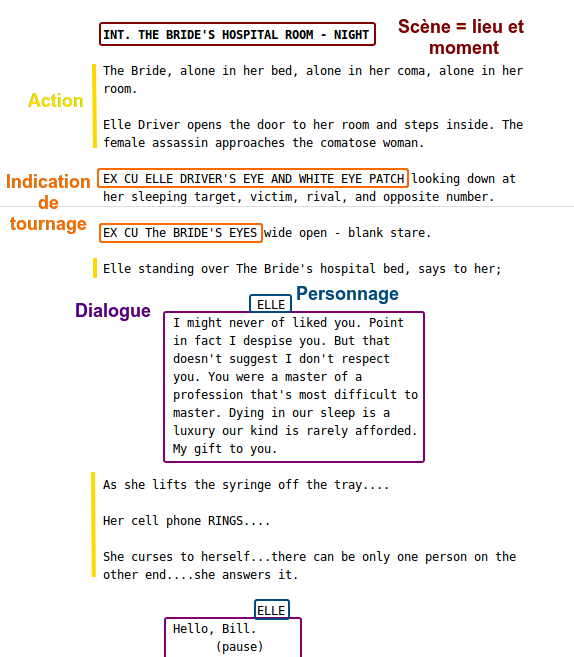
\includegraphics[width=0.7\textwidth]{images/ScriptExample-v1.png}
\caption{Extrait du script de Kill Bill écrit et réalisé par Quentin Tarantino}
\label{img:intro:script} 
\end{figure}

% des réécritures de documents et des mises à jours qui pourraient être réalisées par des machines, des informations qui pourraient être transmises automatiquement à travers un réseau numérique d'information


% un vocabulaire bien défini qui fait l'objet de nombreux dictionnaires, donc prêt à être formalisé


% des équipes qui sont réduites lors de tournage en extérieur




%%%%%%%%%%%%%%%%%%%%%%%%%%%%%%%%%%%%%%%%%%%%%%%%%%%%%%%%%%%%%%%%%%%%%%%%%%%%%%%%%%%%%%%%%%%%%%%%%%%
\subsection{Besoins Métiers}\label{sec:besoins}
\e{
Face à une numérisation qui fragmente les contenus, une mise en réseau qui facilite la fabrication amateur, intensifie la circulation de ces fragments (\ref{sec:motiv}), la production audiovisuelle rencontre de nouveaux défis qui remettent en jeu son organisation et sa manière de se représenter le monde. 
Ainsi d'une part la fragmentation ne doit pas mettre en péril la cohérence de l'ensemble et d'autre part, la circulation des contenus ne doit pas compromettre l'exploitation future du tout ou des parties. 
L'ouverture d'une chaîne de production à des acteurs tiers implique de clarifier les attendus de chacun. 
Lorsqu'il s'agit de faire fabriquer ou de récupérer du contenu, il devient nécessaire pour le client de décrire la commande de contenu au fournisseur, de même que le fournisseur doit décrire à son client le contenu livré pour faciliter son exploitation. 
Ainsi, on souhaite adjoindre aux contenus des descriptions qui permettent de faciliter leur recherche et leur manipulation.
}


Pour les professionnels de la production audiovisuelle, le défi porte à la fois sur l'organisation de leur chaîne de production et sur la gestion de leurs produits :
\begin{liste}
	\item[(1)] \g{comment transformer la chaîne de production afin de l'ajuster à la diversification des formes de fabrication et de distribution des contenus, mais aussi aux changements dans les pratiques de consommation des audiences ?}

	\item[(2)] \g{comment passer d'une gestion de fichiers à une gestion de contenus audiovisuels considérés comme des objets numériques fragmentés dont il s'agit de garantir l'autonomie dès leur conception et jusque dans leurs différents cadres d'exploitation ?}
\end{liste}

% Problèmes métiers ? Tant que ça ne devient pas une solution, mais des tendances à prendre en compte 

On peut ensuite détailler ces défis en objectifs plus précis :
\begin{liste}
	\item[(1a)] \e{accorder contribution amateur et production professionnelle pour fabriquer ou valoriser du contenu.}

	L'amélioration croissante des capteurs des appareils multimédia ajoutée aux capacités de communication offrent au grand public de plus en plus de manières de participer aux processus de fabrication ou de diffusion des contenus.
	Les possibilités accrues de participation au processus médiatique (participation à l'émission, envoi de contenu, propagation via ses contacts, commentaires etc.) valorisent le spectateur, le contenu et la plate-forme de diffusion (comme d'une certaine manière peut le faire le bouche à oreille).

	De manière générale, l'intégration de contenus externes dans une chaîne de production professionnelle ne s'envisage  qu'à partir d'un certain niveau de qualité du contenu livré.  
	Paradoxalement, dans certains cas les signes d'une production amateur (tremblements, caméra à l'épaule etc.) peuvent être revendiquées comme des marque de style qui suggère une collaboration avec le public ou une proximité avec une réalité éloignée des images diffusées par les médias.
	Ainsi, les professionnels souhaitent encadrer plus ou moins fortement la production amateur par des indications, recommendations, obligations.\\


	\item[(1b)] \e{créer de nouvelles étapes dans la chaîne visant à réutiliser les contenus existants et les adapater à de nouveaux modes de consommation.}

	L'augmentation de l'offre de contenus accessibles aux spectateurs (chaînes, enregistrements, balladodiffusion, vidéo à la demande etc.) se traduit par une mise en concurrence accrue des contenus diffusés par les professionnels.
	Le contrôle de l'offre n'étant plus atteignable, il faut adopter de nouvelles stratégies de valorisation des contenus produits ou diffusés pour maintenir leur visibilité et leur rentabilité. 
	Une autre approche consiste à fournir un service de recommandation aux spectateurs et ainsi rentrer dans une démarche de fidélisation. 

	Par ailleurs, l'augmentation des terminaux de lecture multimédia et leur portabilité offrent de plus en plus d'occasions aux spectateurs de consommer des contenus. 
	Par exemple, les situations de mobilités peuvent impliquer des capacités de transfert diminués, un écran plus petit, des temps de disponibilités plus courts etc.
	Il semble alors que la production doivent évoluer pour fournir de nouveaux formats ou des formes retravaillées de contenus existants.

	Dans tous les cas, cela implique de se consacrer à des tâches d'éditorialisation des contenus pour répondre aux exigences et aux attentes de ces nouveaux modes de consommation.\\
% \end{liste}


% \begin{liste}
	\item[(2a)] \e{gérer l'intégration de contenu externes, les variations d'un même contenu pour les rattacher à un même objet numérique.} 
	% représentation

	L'utilisation de contenus provenant de sources externes de même que la production de multiples variations d'un même contenu augmente le nombre de ressources à gérer. 
	De plus, les relations entre ces différentes ressources nécessitent d'être clarifiées et explicitées dans le système de gestion. 
	% chaîne éditoriale ? 
	
	Il ne s'agit plus simplement de gérer des fichiers mais un ensemble de fichiers et de données qui constituent un ensemble cohérent et fragmenté que l'on nomme un objet numérique. 
	Cet objet doit intégrer à la fois les diverses sources qui le composent mais aussi des variations correspondants aux exploitations visées, des descriptions et tout ce qui permet de garantir son autonomie. 
	Il doit également s'agir d'un objet \e{métier} car son statut, son organisation, sa sémantique correspondent à la vision d'un métier, à la manière dont il pense le monde. 

	% Ainsi, on ne souhaite plus gérer des fichiers mais des objets numériques qui doivent acquérir un statut, une sémantique correspondant à la manière dont les métiers de la production les considèrent.\\
	% qui possède une valeur et une sémantique propre à un contexte d'usage. 	


	\item[(2b)] \e{associer des descriptions aux contenus pour faciliter leur exploitation dans un environnement numérique.}
	% description

	L'augmentation des contenus audiovisuels en circulation, la diversification de leurs modes d'exploitation compliquent la gestion des contenus.  
	Afin de favoriser la réutilisation de ces contenus, il faut pouvoir leur attacher des informations pertinentes pour les professionnels qui les manipulent. 
	La description du contenu peut varier suivant les besoins de chaque métier impliqué dans la chaîne de production. 
	Les opérations n'étant pas les mêmes, les descriptions de ces opérations varient donc également et sont nécessaires pour faciliter la réutilisation du contenu. 
	%de manière à faciliter modalités d'exploitation envisagées  

	Lorsque la réutilisation et production s'entremêlent, il est également nécessaire de construire les descriptions en même temps que le contenu. 
	De cette manière on récupère ou on réévalue l'information à mesure de l'avancée dans la chaîne. 

	Cela nécessite d'informatiser l'étape de pré-production de la chaîne et de modéliser les informations utilisées par les professionnels. 
	%commencer plus tôt, avoir plusieurs niveaux/types de description, raccrocher les bons éléments à la représentation de l'objet numérique
	
	%et embarquent des descriptions explicitant leurs modalités d'exploitation.

\end{liste}

\e{
En guise de synthèse, nous pouvons dire qu'il s'agit de constituer des objets audiovisuels autonomes dans les chaînes de production audiovisuelle. 
Nous précisons ce caractère autonome, car ces objets seront porteurs de leur propre description et associés à des connaissances sur l'organisation de la chaîne de production dans lesquels ils évoluent.
Ainsi, ces objets audiovisuels pourront être (ré)introduits à n'importe quelle étape d'une chaîne de production et fourniront aux contributeurs concernés des informations propres à faciliter leur (ré)utilisation.
}
	% \item \eg{valoriser et éditorialiser les contenus existants pour les rendres plus visibles, plus attrayants auprès des audiences ciblées.}
	% L'augmentation de l'offre de contenus accessibles aux spectateurs (chaînes, enregistrements, balladodiffusion, vidéo à la demande etc.) se traduit par une mise en concurrence accrue des contenus diffusés par les professionnels.

	% Le contrôle de l'offre n'étant plus atteignable, il faut adopter de nouvelles stratégies de valorisation des contenus produits ou diffusés pour maintenir leur visibilité et leur rentabilité. 
	% Une autre approche consiste à fournir un service de recommandation aux spectateurs et ainsi rentrer dans une démarche de fidélisation. 
	% Cela implique de se consacrer à des tâches d'éditorialisation des contenus pour des audiences plus ciblées.
	
	% \item \eg{produire de nouvelles formes de contenus ou adapter les rmes existantes pour satisfaires aux nouveaux modes de distribution/consommation.}
	% L'augmentation des terminaux de lecture multimédia et leur portabilité offrent de plus en plus d'occasions aux spectateurs de consommer des contenus. Par exemple, les situations de mobilités peuvent impliquer des capacités de transfert diminués, un écran plus petit, des temps de disponibilités plus courts etc.
	% Il semble alors s'ouvrir une place pour de nouveaux formats ou des formes retravaillés de contenus existants. 
	% Il s'agit de faire de la production multi-support et d'adapter les contenus en fonction des conditions de distribution et de l'audience visé (réutilisation).
	
	% \item \eg{articuler la contribution amateur avec la chaîne de production professionnelle.}
	% L'amélioration croissante des capteurs des appareils multimédia ajoutée aux capacités de communication offrent au grand public de plus en plus de manières de participer aux processus de fabrication ou de diffusion des contenus.
	% Les possibilités accrues de participation au processus médiatique (participation à l'émission, envoi de contenu, propagation via ses contacts, commentaires etc.) valorisent le spectateur, le contenu et la plate-forme de diffusion.

	% Cependant, il faut être capable d'intégrer ces contributions externes au sein de la production professionnelle en les encadrant plus ou moins fortement, par des indications, recommendations ou des contraintes.

	% \item \eg{gérer les objets audiovisuels dès le début et tout au long de leur cycle de vie.}
	% %
	
	% Une circulation plus importante des contenus implique de trouver un moyen de gérer non plus des fichiers mais des objets numériques qui unifient plusieurs variations d'un même contenu et embarquent des descriptions explicitant leurs modalités d'exploitation.



% numériser => (a) fragmenter + (b) mettre en réseau => (a) besoin de conserver la cohérence de l'ensemble + (b) besoin d'autonomiser pour une future situation d'usage








%%%%%%%%%%%%%%%%%%%%%%%%%%%%%%%%%%%%%%%%%%%%%%%%%%%%%%%%%%%%%%%%%%%%%%%%%%%%%%%%%%%%%%%%%%%%%%%%%%%
% \newpage
\section{Problèmes}\label{sec:prob}



%%%%%%%%%%%%%%%%%%%%%%%%%%%%%%%%%%%%%%%%%%%%%%%%%%%%%%%%%%%%%%%%%%%%%%%%%%%%%%%%%%%%%%%%%%%%%%%%%%%
\subsection{Problèmes métiers}\label{sec:pmetiers}
% Nos champs d'applications sont : 
% Prenant acte des besoins de la production audiovisuelle nous distinguons deux problèmes métiers (1) identifier le(s) niveau(x) de fragmentation et (2) le(s) type(s) de description susceptibles de favoriser la fabrication mixte, la circulation et la réutilisation des contenus.
% Ces problèmes remettent en cause à la fois la représentation classique des contenus et leur description. 
% de manière à faciliter (1) la production mixte amateur-professionnel et (2) leur réutilisation dans de nouveaux contextes d'exploitation.
% l'informatisation du début de la chaîne de production, préproduction 
% l'inscription formelle de l'écriture audiovisuelle ?

\e{
L'objectif central qui se pose à la production audiovisuelle est de constituer des objets audiovisuels autonomes et donc (ré)utilisable à n'importe quel étape de la chaîne. 
Or, dans la chaîne de production classique les programmes n'émergent qu'à la fin de la chaîne et sont gérés d'une pièce. 
Il n'y a pas forcément de place pour les éléments de contenu intermédiaires, et c'est justement à la modélisation de ces fragments que l'on s'attaque. 
Ces fragments doivent devenir des éléments documentaires qui possèdent leur unité propre de même que les objets finis que sont les programmes. 
Une des difficultés réside dans cette articulation entre des fragments et le tout ou l'ensemble que constitue les programmes. 
Par ailleurs, il existe des problèmes sous-jacents à cette fragmentation documentaire : 
}
\begin{liste}
	\item \e{identifier quels niveaux de fragments peuvent prétendre à ce genre de transformation}.
	Si le numérique permet de fragmenter à l'envie, il faut cependant prendre en compte les pratiques du métier pour identifier les niveaux de fragmentation pertinents ou déjà utilisés dans le métier mais non modélisés.
	Par exemple, la prise de vue est le résultat d'une activité de tournage, pour autant elle ne constitue pas un objet éditorial comme peut l'être une interview.
	De plus, il s'agit également de déterminer comment manipuler ces fragments comme des objets à part entière sans compromettre l'articulation de l'ensemble. 
	Par exemple, une interview peut s'intégrer dans un journal télévisé ou bien un reportage dans des versions plus ou moins courtes. 
	Pour autant, il s'agit du fruit d'une même activité, simplement le montage, et donc le résultat, est différent suivant le programme dans lequel l'interview s'insère.\\
	
	\item \e{identifier quelles informations et connaissances doivent être rattachées à ces fragments pour les rendre autonome}.
	D'une manière similaire à la démarche pour les objets entiers, certaines connaissances, notamment relatives au contexte de production, doivent être attachées au fragment pour garantir sa réutilisation et sa cohérence. 
	En reprenant l'exemple de la prise de vue, on peut lui associer le bout de script qui a prescrit ce qu'elle devait montrer. 
	Si l'on pousse encore cette logique, il faut également incorporer le document qui définit le programme pour lequel on a tourné cette prise de vue, la personne qui l'a effectuée, les équipements utilisés etc. 
	Ainsi, on étend la modélisation de l'objet audiovisuel à son contexte de production et tout ce qui renforce les possibilités de recherche, de manipulation, de gestion et de transformation de ces objets. 
	De plus, s'ajoute à cela la question de la collecte de ces informations. 
	En effet, la saisie de ces informations au sein d'un système d'information et leur utilisation par les acteurs de la chaîne n'est pas une simple formalité.
	Ce problème pousse également dans le sens d'une modélisation plus contextuelle, de manière à proposer un environnement de travail adapté et utilisable aux contributeurs de la chaîne.\\
	
	% \item \e{}.
\end{liste}


% Notre problème se situe dans le croisement de la représentation des contenus et la représentation des activités humaines qui construisent, manipulent, éditent, transforment, publient et documentent ces contenus. 
% Cet angle de recherche nous amène donc à considérer non pas le contenu audiovisuel dans son ensemble, une fois terminé et validé, mais la construction de tout ces fragments qui le composent. 
% Il nous faut aussi considérer, non pas seulement le contenu audiovisuel, mais aussi d'autres informations, d'autres documents qui constituent son contexte de production, dans un sens très général. 
% Chaque prise de vue constitue donc un objet à représenter en tant que tel, tout autant que le bout de script qui a prescrit ce que cette prise de vue devait montrer. 
% Si l'on pousse encore cette logique, on peut alors représenter de même le document qui définit le programme pour lequel on a tourné cette prise de vue, la personne qui l'a effectué, les équipements utilisés etc. 
% Ainsi, on étend la représentation du contenu à son contexte de production entendu comme toutes les informations qui renforceront les possibilités de recherche, de manipulation, de gestion et de transformation de ces contenus. 

%%%%%%%%%%%%%%%%%%%%%%%%%%%%%%%%%%%%%%%%%%%%%%%
\subsection{Problèmes scientifiques}\label{sec:scien}
Au fur et à mesure que la circulation des contenus s'intensifie, il y a un besoin grandissant de faciliter l'échange d'information tant à la fois sur le plan informatique, que sur le plan humain. 
De plus, l'ouverture de la chaîne de production à de nouveaux contributeurs (amateurs et professionnels) ne fait qu'accentuer la disparité des connaissances et des systèmes utilisés. 
Afin de construire une compréhension commune à tous les contributeurs au cycle de vie, on fabrique un modèle conceptuel capable d'intégrer et de mettre en relation leurs connaissances. 
Il s'agit là d'un apport par rapport à la situation existante où le consensus n'existait pas, ou alors de manière éphémère, locale au sein d'une équipe.
L'objectif est de fluidifier les échanges d'information et de contenus en formalisant les connaissances utilisées pour :
\begin{problemes}{LightGoldenrodYellow}
\begin{liste}
% modéliser tous les objets de la chaîne de production audiovisuelle
	\item[(A)] \g{modéliser les objets construits au fil de la chaîne de production audiovisuelle}.
	\item[(B)] \g{modéliser les connaissances sur ces objets} (descriptions, contexte de production, contribution au cycle de vie).
	% \item[(B)] décrire les objets audiovisuels
	% \item[(C)] représenter la contribution de chacun des acteurs au cycle de vie des objets audiovisuels
\end{liste}
\end{problemes}

\e{
Ainsi, notre problème de recherche général s'articule autour de la modélisation des connaissances et des informations que les contributeurs construisent, utilisent, échangent au cours du cycle de vie des objets audiovisuels. 
Cette modélisation constitue une première étape dans la mise en place d'un système d'information servant à mieux gérer les objets audiovisuels et médier la communication entre systèmes informatiques tout autant qu'entre contributeurs humains.
Après avoir numérisé les contenus audiovisuels, on souhaite transformer chaque élément les composant en objet documentaire et documenter leur cycle de vie.\\}



\g{(A)} Le problème est d'organiser la gestion des objets audiovisuels en proposant une modélisation capable de faciliter leur identification, leur manipulation et leur réutilisation tout au long de leur cycle de vie. 
En particulier,	l'objet audiovisuel professionnel est produit de manière collective, chaque contributeur apportant un élément à l'ensemble. 
Ces contributions doivent donc pouvoir être identifiées comme appartenant à un ensemble, de même que chaque élément doit pouvoir être considéré pour soi afin d'être intégré dans un autre ensemble (réutilisation).

Pour cela on adopte une représentation des différents niveaux d'abstraction des objets audiovisuels numériques de façon à rétablir les liens entre les différentes versions ou copies d'un même contenu, quelque soit la nature des variations entre elles (encodage, format d'encapsulation, montage, finition, langue etc.).
La distinction entre différents niveaux de modélisation (technique, esthétique, éditorial etc.) doit permettre de construire une représentation dynamique de l'objet audiovisuel qui suit l'avancement du processus de production.\\
% La distinction entre différents niveaux de modélisation (technique, esthétique, éditorial etc.) doit permettre de construire une représentation de l'objet audiovisuel au fur et à mesure de l'avancement du processus de production.\\


\g{(B)} Le problème est d'attacher plusieurs types de connaissances aux objets audiovisuels de manière à les rendre autonomes dans leur circulation et leur réutilisation. 
Afin de faciliter l'échange d'information et la réutilisation des objets audiovisuels entre différents contextes, il faut modéliser des connaissances sur ces objets qui sont parfois déjà existantes mais non formalisées, ou bien qu'il faut rendre compréhensibles.
En effet, l'échange d'informations dans la production audiovisuelle est primordial et s'effectue entre métiers ou organisations différent(e)s, voire avec des amateurs. 
En particulier, on souhaite s'appuyer sur le vocabulaire de l'écriture filmique utilisé dans des documents de préproduction pour spécifier les résultats attendus de la production.
L'information contenue dans ces documents est importante mais repose sur des conventions plus ou moins tacites qu'il faut expliciter pour les professionnels, expliquer pour les amateurs.
La formalisation de ces éléments devra donc pouvoir être lu et modifié tout au long du cycle de vie des objets audiovisuels par tout types de contributeurs.

% échange d'info, adaptation par l'explicitation du vocabulaire et la contribution au cycle de vie
La formalisation de l'écriture filmique permettra d'adapter la présentation de l'information en fonction des connaissances, de l'implication du contributeur dans la chaîne (rôle, tâche, niveau de compétences etc.), de son référentiel professionnel ou linguistique. 
Il s'agit alors d'établir des correspondances entre les connaissances connues par le lecteur d'une information et celles utilisées par la personne qui l'a exprimée.
Ainsi, d'une part on explicite l'expression de l'information, ce qui permet l'adpatation, et facilite son interprétation ultérieure.
Le processus prend tout son sens lorsqu'il s'agit de traduire un concept de la réalisation audiovisuelle pour guider un amateur dans son tournage.
% Par exemple, l'action écrite par l'auteur et transformé en scène par le réalisateur, doit ensuite être tourné un caméraman, des acteurs etc. 


% réutilisation, attachement des connaissances pertinentes pour manipuler ou exploiter chaque fragment ou l'objet en entier
De plus, les descriptions utilisées, en plus de permettre de spécifier le résultat attendu de la production, doivent permettre de faciliter la recherche, la manipulation et la réutilisation des objets audiovisuels.
Pour cela, il faut articuler ces connaissances aux objets et aux fragments qui les composent. 
Le vocabulaire de l'écriture filmique sera également précieux, puisqu'il nous donne une unité de base, le plan, ainsi que ses caractéristiques qui permettent de le distinguer des autres. 
La recherche dans des dépôts de contenus se fera ainsi de manière similaire à la commande de contenu à d'autres contributeurs, qu'ils soient professionnels ou amateurs.



% Il s'agit donc de définir un modèle de description susceptible d'être utilisé par les contributeurs professionnels ou amateurs, à toutes les étapes de la chaîne de production. 


% Afin de décrire les contenus, on souhaite s'appuyer sur le vocabulaire de l'écriture audiovisuelle utilisé dans les différentes étapes de la chaîne et notamment dès la préproduction. 
% Cette écriture repose sur un vocabulaire des techniques de réalisation audiovisuelle (prise de vue, transition, composition de l'image etc.) renvoyant à des effets largement connus dans le milieu de l'audiovisuel et chez les cinéphiles. 
% L'écriture est utilisée avant la fabrication du contenu pour la spécifier, puis pendant la fabrication pour enregistrer les différences. 
% Une formalisation de ce vocabulaire permettrait de construire une description textuelle d'un contenu à partir d'une description objective de la réalisation (réglages des appareils, position des acteurs etc.).\\



% \g{(C)} Le problème est de représenter et faciliter l'échange d'information entre des contributeurs hétérogènes dans leurs connaissances et leur implication dans la chaîne de production.
% Une première diffculté réside dans l'articulation entre les connaissances des contributeurs qui expriment l'information et ceux qui l'interprèteront.
% La seconde diffculté consiste dans l'articulation des représentations du cycle de vie, de l'objet audiovisuel et des descriptions qui leurs sont associées. 
% En effet, chaque contributeur peut participer à la constitution d'informations associées au contenu en cours de sa production.
% Ces informations varient en fonction de l'implication du contributeur dans la chaîne (rôle, tâche, niveau de compétences etc.). 
% De plus, les informations construites à un moment sont susceptibles d'être utilisées plus tard dans la chaîne, par un contributeur ne partageant pas forcément les mêmes connaissances ou le même référentiel professionnel ou linguistique.

% On cherche alors à réaliser une adaptation de la forme d'expression de ces informations afin de faciliter le déroulement du processus de production. 
% Dans un premier temps, on explicite les connaissances utilisées par un premier utilisateur pour exprimer une information. 
% Ensuite, on établit une correspondance avec les connaissances connues d'un autre utilisateur et on adapte au besoin la forme de d'expression de cette information pour faciliter son interprétation. 
% L'adpatation qui en résulte prend tout son sens lorsqu'il s'agit de traduire un concept de la réalisation audiovisuelle pour guider un amateur dans son tournage.


%%%%%%%%%%%%%%%%%%%%%%%%%%%%%%%%%%%%%%%%%%%%%%%
% \section{Positionnement Disciplinaire (n,i)}\label{sec:posd}
% [Ingénierie des connaissances ; Media Asset Management ; Gestion électronique de Documents ; Ingénierie documentaire]
% ingénierie des connaissances (représentation des connaissances) ingénierie des inscriptions numériques de connaissances, dont les documents
% ingénierie documentaire (modélisation des documents propres à la production audiovisuelle)
% indexation et gestion des connaissances (description des contenus audiovisuels)
% la ged s'occupe de la gestion de documents, nous proposons de gérer des fragments de documents, de gérer leur construction en plusieurs étapes, par plusieurs acteurs et dans le cadre de différentes missions.

% Pour définir cet ensemble d'informations qui forment le contexte de production, nous nous sommes appuyés sur les partenaires du projet MediaMap. 



% des réécritures de documents et des mises à jours qui pourraient être réalisées par des machines, des informations qui pourraient être transmises automatiquement à travers un réseau numérique d'information
% un vocabulaire bien défini qui fait l'objet de nombreux dictionnaires, donc prêt à être formalisé
% des équipes qui sont réduites lors de tournage en extérieur

% à mettre dans le pos. disciplinaire, comment on aborde les problèmes posées
% [Nous avons ainsi dégagé plusieurs perspectives métiers qui nous ont servi de guide pour identifier les échanges d'informations les plus importants ainsi que le vocabulaire utilisé pour les exprimer. 
% Chacune de ces perspective possède un objectif propre et des spécificités, cependant il apparaît qu'un langage commun est utilisé par tous les acteurs de la production. 
% En se concentrant sur la description d'un contenu existant ou à venir, ce langage permet à ces acteurs de communiquer entre eux. Le réalisateur qui spécifie un attendu dans son script, les caméraman qui réalisent le cadrage, les opérateurs lumières etc. 
% Tous utilisent ce langage pour imaginer le résultat à produire et en déduire les gestes à opérer. 
% Les usages n'étant jamais complètement figé, chaque organisation développe ses propres idiomatismes de langage. 
% Dans ce cas, la collaboration entre organisations impliquent de pouvoir réaliser des ajustements dans l'expression de la description du contenu. 
% De même, la collaboration avec des contributeurs amateurs soulève un problème de compréhension de ce langage (et donc de l'attendu) mais aussi de connaissances des gestes à opérer (pour produire le résultat attendu).
% Ainsi, à mesure que la circulation des contenus s'intensifie, que les besoins de collaboration augmentent, naît un besoin grandissant d'explicitation des échanges d'information afin de dégager une vue d'ensemble de la chaîne de production, de ses acteurs, de leurs interactions, de leurs produits. 

% Notre proposition consiste à modéliser ces éléments et à en informatiser l'accès de manière à fluidifier les échanges de contenus et faciliter la compréhension des informations afférentes.] 


% \cleardoublepage





%%%%%%%%%%%%%%%%%%%%%%%%%%%%%%%%%%%%%%%%%%%%%%%%%%%%%%%%%%%%%%%%%%%%%%%%%%%%%%%%%%%%%%%%%%%%%%%%%%%
%%%%%%%%%%%%%%%%%%%%%%%%%%%%%%%%%%%%%%%%%%%%%%%%%%%%%%%%%%%%%%%%%%%%%%%%%%%%%%%%%%%%%%%%%%%%%%%%%%%
\part*{État de l'art}
\addcontentsline{toc}{part}{État de l'art}
%%%%%%%%%%%%%%%%%%%%%%%%%%%%%%%%%%%%%%%%%%%%%%%%%%%%%%%%%%%%%%%%%%%%%%%%%%%%%%%%%%%%%%%%%%%%%%%%%%%
%%%%%%%%%%%%%%%%%%%%%%%%%%%%%%%%%%%%%%%%%%%%%%%%%%%%%%%%%%%%%%%%%%%%
%%%%%%%%%%%%%%%%%%%%%%%%%%%%%%%%%%%%%%%%%%%%%%%%%%%%%%%%%%%%%%%%%%%%
%%%%%%%%%%%%%%%%%%%%%%%%%%%%%%%%%%%%%%%%%%%%%%%%%%%%%%%%%%%%%%%%%%%%
%%%%%%%%%%%%%%%%%%%%%%%%%%%%%%%%%%%%%%%%%%%%%%%%%%%%%%%%%%%%%%%%%%%%
\chapter{Outils de modélisation}\label{c:omod}


% pourquoi on parle de SOC ? Parce qu'on souhaite représenter des objets audiovisuels, leur production, leur description et que ceci ne peut se faire sans une représentation du vocabulaire utilisé dans la production audiovisuelle. 

Dans le cadre de la production audiovisuelle collaborative, qui implique à la fois des amateurs et des professionnels, un des enjeux que nous avons noté (\ref{sec:scien}) est de rendre plus compréhensible l'échange d'informations entre contributeurs. 
D'une part, nous avons des practiciens professionnels utilisant un ou plusieurs vocabulaires métiers suffisamment définis pour que l'on puisse en faire des dictionnaires (\cite{Journot2008}; \cite{Pinel2008}). 
Ces personnes font usage de la langue d'une manière précise, régie par des conventions et portée par une conception de la production audiovisuelle et de ses objets, que l'on suppose stabilisée, au moins localement (au sein d'un même pays, d'une même école de pensée, organisation, équipe etc.).
Toutefois, on s'attend à des variations dans les usages de la langue, au même titre que l'on suppose qu'il existe des variations entre pratiques des gens du métiers.
Cependant, il semble qu'il s'agit seulement de variations et qu'il soit possible alors d'identifier les éléments communs et distincts.

D'autre part, les amateurs, quant à eux, n'ont pas le support de ces conventions travaillées au quotidien.
Ils sont, au mieux, des intermittents éclairés qui ont saisi le sens d'éléments de langage propres aux métiers (par des lectures, des rencontres, des formations etc.). 
Il faut donc supposer qu'il y a tout à expliquer à ces amateurs, plutôt que de parier sur leur compréhension innée des métiers de la production audiovisuelle.
En particulier s'il s'agit de demander du contenu à des amateurs sous la forme d'un script de tournage, il faudra alors trouver un moyen d'expliciter cette commande et d'expliquer ou d'assister sa réalisation. 

Ainsi, l'écart entre collaborateurs (qu'ils soient tous professionnels, ou un mélange d'amateurs et de professionnels) peut se situer sur différents niveaux : 
\begin{liste} 
	\item au niveau du vocabulaire métier, comme les mots utilisés dans le script pour désigner tel ou tel type de plan etc. 
	Dans le cas d'amateurs, il faut supposer que ces mots sont inconnus ou méconnus ; dans le cas de professionnels, on préfèrera expliciter le vocabulaire afin d'éviter toute confusion. 
	
	\item au niveau des connaissances et de la manière de conceptualiser le métier, le cycle de production et ses objets. 
	Là encore, un amateur ne connaît pas ou très peu les détails classiques des méthodes de production professionnelle. 
	De plus, la production audiovisuelle étant organisée en projets distincts, les méthodes peuvent fortement varier entre la production d'un documentaire et d'une émission de variétés. 
	Chaque genre, chaque équipe aura donc ses propres objets, ses propres méthodes qu'il faut alors expliciter aux autres professionnels pour s'assurer de leur collaboration. 

	\item sur le plan pratique, il faut également remarquer que les compétences peuvent également varier fortement entre métiers, suivant les genres de production audiovisuelle. 
	Ainsi, en plus d'expliciter les échanges d'informations, il serait également souhaitable de proposer une assistance aux collaborateurs amateurs ou professionnels pour s'assurer que le résultat produit correspond bien à l'attente initiale. 	
\end{liste}


Nous présentons dans une première section un exemple de commande de tournage qui illustre ces différents écarts en impliquant des communautés d'amateurs et de professionnels (\ref{sec:cdcf}). 
Ce scénario d'usage nous permet de préciser les besoins en modélisation exprimées précédemment (\ref{sec:prob}).
Notamment, il apparaît nécessaire de représenter à la fois la ou les conceptualisation(s), le(s) vocabulaire(s) utilisé(s) ainsi que les résultats attendus par les acteurs de la chaîne de production audiovisuelle. 
Ainsi, nous nous intéresserons à l'utilisation de divers Systèmes d'Organisations de Connaissances (SOC, \cite{Zacklad2010}) pour mettre en place un partage d'information normalisée. 
Après un retour sur les définitions principales que nous utiliserons, nous examinerons les langages, modèles et normes existants qui permettent de représenter des SOC (\ref{sec:defs}).
La distinction entre terminologie et ontologie nous nous permet de détailler le fonctionnement d'une méthode de construction d'ontologie différentielle (\ref{sec:construction}).
Enfin, nous présenterons les langages permettant de représenter ces SOCs (\ref{sec:mods}). 

%Dans une seconde partie, nous examinerons les modèles de l'audiovisuel existants.




%%%%%%%%%%%%%%%%%%%%%%%%%%%%%%%%%%%%%%%%%%%%%%%%%%%%%%%%%%%%%%%%%%%%
%%%%%%%%%%%%%%%%%%%%%%%%%%%%%%%%%%%%%%%%%%%%%%%%%%%%%%%%%%%%%%%%%%%%
\section{Cahier des charges fonctionnel (n)}\label{sec:cdcf}


%%%%%%%%%%%%%%%%%%%%%%%%%%%%%%%%%%%%%%%%%%%%%%%%%%%%%%%%%%%%%%%%%%%%
\subsection{Scénario de commande de tournage}\label{sec:scenar}
Considèrons comme cas d'étude une commande de tournage en vue de réaliser des reportages sur des évènements culturels de type concert ou opéra. 
Il met en jeu trois communautés en collaboration :

\begin{itemize}
	\item la RTBF (Radio Télévision Belge Francophone) établit des commandes de contenu dans un jargon métier propre. Son objectif est d'externaliser dès que possible la réalisation de la commande. Cela implique une compréhension commune sur le contenu à réaliser qui passe par un accord sur la manière de décrire la commande. 
	
	\item le contenu commandé est tourné soit par la VRT (Radio-Télévision Flamande) qui utilise un jargon différent de la RTBF, soit des amateurs qui ne connaissent pas les concepts de la réalisation audiovisuelle. Dans le premier cas, la conceptualisation est commune, seuls les termes changent. Dans le second cas, il s'agit d'expliquer et d'illustrer les concepts utilisés \\
\end{itemize}

Le développement d'une application d'assistant de tournage pour guider les amateurs paraît souhaitable pour amener le contenu filmé à un niveau de qualité exploitable. 
Il faut cependant faire la distinction entre les propositions de dépôt spontané de contenu (comme le pratique une chaîne d'information telle que BFM\footnote{La rubrique témoins BFM permet à un utilisateur de déposer des photos ou vidéos sur le site. 
Après modération, le contenu est diffusé et peut même faire l'objet d'une vente. Voir http$:$//temoins.bfmtv.com/}) et les appels à contribution où le professionnel passe commande auprès d'amateurs en détaillant ses exigences. 

Dans ce dernier cadre, on souhaite fournir un plan de tournage au caméraman afin de guider sa prise de vue. 
Le plan de tournage est construit à partir de recommandations rédigées par un réalisateur (position, cadrage, lumière, etc.) utilisant un vocabulaire métier. 
L'originalité de l'application est d'adapter l'information présentée au caméraman suivant ses capacités (amateur, professionnel) ou son employeur si c'est un professionnel travaillant dans une tierce organisation. 
On suppose ainsi que malgré quelques variations dans le vocabulaire utilisé, les professionnels de l'audiovisuel utilisent les mêmes concepts pour décrire le contenu. 
Par exemple, la notion de cadrage fait appel à des concepts de valeurs de plan indiquant la portion visible d'un personnage à l'écran (voir Figure \ref{img:intro:script}, page \pageref{img:intro:script}).
Un \textit{plan américain} indique ainsi que le personnage principal est cadré de la tête jusqu'au dessus des genoux. 
Le terme est utilisé en Europe en rappel à son emploi caractéristique dans les films américains des années 1910-1940, notamment dans les westerns où il permettait de montrer l'ensemble du pistolet à la ceinture des personnages\footnote{Roger Boussinot, l'Encyclopédie du Cinéma, Bordas.}. 
Ce cadrage est aussi appelé \textit{plan 3/4} et en anglais 3/4 shot, medium-long shot ou american shot pour traduire l'expression popularisée en Europe. 
Si le terme utilisé varie suivant le lieu et la littérature de référence, la définition de ce type de cadrage est sans équivoque. 

%=============
% \begin{figure}[htb]
% \centering
% 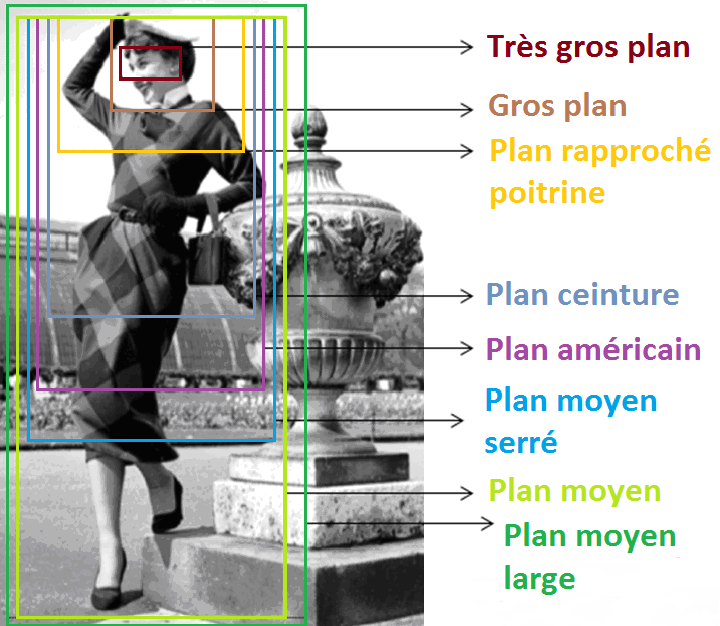
\includegraphics[width=0.5\textwidth]{./images/ValeurPlan-v1.png}
% \caption{Différentes valeurs de plan pour le cadrage d'un personnage à l'écran}
% \label{fig:cadrage}
% \end{figure}
%=============

Les amateurs quand à eux ignorent ces concepts et n'ont pas été initiés à ces pratiques. Ils ont donc besoin d'explications et d'illustrations pour comprendre les recommandations du réalisateur. 
Dans le cas du cadrage, une illustration graphique est d'autant plus pertinente. 
L'enjeu se situe donc dans la collaboration entre un prescripteur et un opérateur qui doivent s'accorder sur le contenu à produire malgré la différence de vocabulaire. 
% Un exemple des différences de présentation entre amateur et professionnel est illustré figure \ref{fig:prescription}.


% %%=============
% \begin{figure}[htb]
% \centering
% \includegraphics[width=0.3\textwidth]{./images/ShootingRecommandation-v1.png}
% \caption{Exemple de prescription de tournage à destination de professionnels (en haut) ou d'amateurs (en bas)}
% \label{fig:eda:prescription}
% \end{figure}
% %%=============


%%%%%%%%%%%%%%%%%%%%%%%%%%%%%%%%%%%%%%%%%%%%%%%%%%%%%%%%%%%%%%%%%%%%
\subsection{Besoins en modélisation}\label{sec:bm}
La mise en place d'une telle application nécessite de représenter le vocabulaire de la réalisation audiovisuelle dans toutes ses variations possibles et de le documenter suffisamment afin de le rendre compréhensible pour des novices. 
Cet objectif nous amène à considérer la construction d'une ressource termino-ontologique. L'ontologie permet de représenter les concepts partagés par les professionels de la réalisation audiovisuelle et la terminologie permet de capturer les différentes formes d'expression associées à ces concepts. 

La spécificité de notre problématique est de considérer la collaboration de communautés hétérogènes par leur degré de compréhension des concepts ou leur utilisation de la terminologie. 
Ceci nous amène à envisager la terminologie comme un moyen d'associer à des éléments ontologiques (concept, relation, instances) une chaîne lexicale ou des ressources média. 
Chaque chaîne ou ressource s'adresse en particulier à une communauté dont les membres partagent une capacité d'interprétation commune. 
Il n'existe donc plus une terminologie de référence par langue, mais des terminologies pour chaque communauté d'utilisateurs. 
On remarquera que notre acception de la terminologie sert bien à normaliser les pratiques linguistiques entre les membres d'une même organisation. 
En plus de cela, elle permet de fixer la manière de s'adresser à d'autres communautés.

Par ailleurs, les types de réalisations sont divers et nécessitent des concepts spécifiques pour être décrits. 
Une fiction se structure en séquences et en scènes alors que les documentaires ou magazines d'information se composent de sujets. 
La variabilité des types de contenu à filmer implique donc de pouvoir étendre le fond conceptuel initial pour représenter de nouveaux usages. 
De la même manière, la collaboration avec de nouveaux partenaires nécessite de pouvoir ajouter de nouvelles terminologies au fond conceptuel existant. 
Ontologie et terminologie doivent se gérer de manière indépendante. A partir de ces besoins, nous définissons maintenant les exigences en terme de modélisation. 

Nos besoins en modélisation peuvent être exprimés par les assertions suivantes:
\begin{enumerate}
	\item[(A1)] la variabilité des pratiques linguistiques des organisations et des communautés implique d'associer plusieurs termes à un même concept. 
	Il n'y a pas de choix des termes préférés par une communauté mais une \textit{correspondance} entre les termes d'une ou plusieurs communautés, quels que soient la langue et le code d'écriture utilisé.
	
	\item[(A2)] la variabilité de compréhension des communautés implique d'associer des explications (chaîne lexicale) ou des illustrations (ressource média) aux concepts afin d'en enrichir la \textit{documentation}. 
	
	\item[(A3)] la variabilité des cas de collaboration implique de pouvoir étendre la conceptualisation initiale ou la terminologie pour s'adapter à de nouvelles pratiques ou de nouvelles communautés. 
	Cela implique une gestion et une \textit{évolution} indépendante de l'ontologie et de la terminologie. 
\end{enumerate}


Dans le cas d'une demande de cadrage en plan américain, la demande est d'abord exprimée dans le jargon de la RTBF puis traduite dans le jargon de la VRT (plan américain pour la RTBF, plan 3/4 pour la VRT) [A1]. 
Ensuite, pour les amateurs, la terminologie est enrichie par des illustrations [A2]. Enfin, un nouveau concept de cadrage est ajouté (plan américain large ou plan moyen serré) [A3] en vue d'une nouvelle coopération avec la VRT. En plus de cela, le problème de la langue (français et flamand) s'ajoute à la question des jargons métiers. 



\section{Définitions des SOC (i)}\label{chap:defs}
%Distinguer entre terme et concept ; dictionnaire, thésaurus, ontologies etc.

\e{
L'objectif de cette section est de clarifier ce qui appartient au domaine de la  linguistique et ce qui relève du domaine conceptuel, en vue d'identifier les notions qui nous serviront à spécifier une solution au cahier des charges dressés dans la section précédente. 
La confusion qui nous intéresse concerne principalement la définition des ontologies par rapport à d'autres SOC tels ques les thésaurus, notamment du fait qu'on utilise parfois les mêmes langages pour les représenter.}

La définition des SOC proposée par \cite{Zacklad2010}, étend celle de \cite{Hodge2000} à \ciel{l'ensemble des formes d'écritures codifiées participant à la description documentaire primaire ou secondaire d'une situation}. 
L'ensemble défini par \citeauthor{Hodge2000} comprend ainsi tout type de :
\begin{liste}
	\item \e{liste de termes} (fichiers d'autorités, glossaires, dictionnaires, répertoires géographiques)
	\item \e{schème de classification/catégorisation} (vedettes-matières, taxonomie)
	\item \e{schème qui se structure par le types de relations qui unit ses membres} (thésaurus, réseaux sémantiques, ontologies). 
\end{liste}

À cela \citeauthor{Zacklad2010} souhaite ajouter des modes de description du contenu émergents ou plus faiblement codifiés comme par exemple les folksonomies. 
Les SOC qui nous intéressent en particulier sont les schèmes structurés par types de relations. 
% pourquoi ? 


\subsection{Thésaurus, terminologie, ontologie}
Dans cette section, nous nous reposerons majoritairement sur les définitions de \cite{bachimont:icc}. Concernant le thésaurus, l'auteur écrit :

\g{Thésaurus :} 
\ciel{
Une organisation de libellés linguistiques selon des relations d'hyperonymie et d'hyponimie. 
Les libellés sont également reliés par des relations dites d'association, qui sont de nature quelconque. 
Même si en pratique les libellés d'un thésaurus correspondent souvent à des termes du domaine, ce n'est pas nécessairement systématique.}

Cette définition situe clairement les thésaurus comme faisant partie du cadre de la linguistique. 
Il s'agit d'un ensemble de mots structurés et reliés suivant leur \e{signification}, c'est à dire leur sens normé ou commun à plusieurs contextes d'usage particuliers (à l'inverse du sens, qui lui varie suivant les usages, \cite{Roche2005}). 
\citeauthor{bachimont:icc} finit sa définition en comparant les mots issus d'un thésaurus aux termes. La distinction se joue à deux niveaux, la stabilité d'écriture du terme (niveau linguistique) et le fait qu'un terme renvoit à un concept (niveau conceptuel) : 

\g{Terme :} 
\ciel{
Une unité linguistique dont le signifié est un concept, c'est-à-dire un signifié normé. 
Le terme se manifeste linguistiquement par une stabilité et régularité de sa forme signifiante.
En particulier, un terme possède des contextes d'occurrence réguliers, obéissant à des canevas morpho-syntaxiques typiques. 
La détection de ces canevas est à la base des outils de détection des termes en corpus. 
Un terme peut posséder des variantes terminologiques.
Dans une optique normative, on détermine une forme préférée.}

Ainsi, plus qu'un repérage des mots (signifiant) utilisés dans un domaine donné, la terminologie s'attache à identifier les signifiés correspondants. 
Au-delà des débats sur les méthodes utilisées pour constituer les couples signifiant-signifié\footnote{L'approche \e{sémasiologique} (initiée par \cite{Bourigault1994}) s'appuie sur l'analyse linguistique d'un corpus de textes pour repérer les couplages signifiant-signifié ainsi que l'organisation conceptuelle sous-jacente. L'identification de ces \e{désignations} est ensuite validée par des experts du domaine. 
Dans une optique différente, l'approche \e{onomasiologique} prend comme appui la modélisation conceptuelle pour nommer ensuite les concepts. On parle alors de \e{dénominations} dont l'objectif est de refléter sans ambiguïté la structure conceptuelle dont elles sont issues.
Une critique faite à la première approche par \cite{Roche2006} est que les relations identifiées entre désignations sont purement linguistiques (hyper/hyponymie, méronymie etc.) et ne se rattachent pas à une structure conceptuelle. Ainsi, l'analyse de texte n'est qu'une première étape dans la constitution d'une terminologie, elle permet d'identifier les usages des mots, mais pas de les raccorder à des concepts. De même, la constitution du corpus va également grandement influer sur les résultats de l'analyse et pose alors un problème de réutilisabilité.}, on cherche à repérer la modélisation conceptuelle sous-jacente d'un domaine, de manière à pouvoir adosser chaque terme à un concept.
À noter que l'inverse n'est pas forcément valable, car il existe des concepts qui n'ont pas d'appelation usuelle et que l'on doit alors désigner par une phrase. 
Une autre conséquence de cette définition est que plusieurs mots peuvent être adossés au même concept.
Il devient alors important de pouvoir expliciter cette équivalence et éventuellement de spécifier un signifié préféré pour le terme.

Cette définition du terme préfigure ainsi la relation qu'entretient la terminologie avec l'ontologie pour \cite{bachimont:icc} : 

\g{Terminologie :} 
\ciel{un recensement et une organisation d'unités linguistiques à l'usage stabilisé et attesté, dont le signifié correspond à un concept du domaine.
La terminologie est l'organisation des termes du domaine.
La terminologie est la face linguistique de l'ontologie, qui en est le côté conceptuel. 
Il n'y a pas une stricte correspondance cependant entre ontologie et terminologie : si tout terme doit correspondre à un concept de l'ontologie, tout concept n'a pas forcément d'usage linguistique régulier attesté.}

De son côté, \cite[\S 2.4]{Roche2005} parle de manière similaire \ciel{[d']un système de termes reflétant une modélisation conceptuelle, [...] plus généralement dénommé \e{système notionnel} [qui] trouve sa raison d'être dans la façon dont nous appréhendons les objets du monde.}
\citeauthor{Roche2005} précise que si les systèmes notionnels ne relèvent pas de la linguistique, ils ne dépassent pas forcément le cadre d'une langue, sauf \ciel{pour des communautés de pratique dont les langues d'usage partagent la même conceptualisation du monde.}.
La distinction est ainsi faite entre les mots d'usage (qui peuvent être polysémiques) et les termes dont on spécifié une forme préférée (signifiant) et qu'on adosse à une signification (signifié normé).  

Concernant les particularismes qui peuvent exister dans chaque communauté, \citeauthor{Roche2005} propose de s'éloigner d'une vision purement normalisatrice. 
Ainsi, sur le plan linguistique, il est possible de rattacher les différents mots d'usages et de préciser leur contextes d'utilisation.
Sur le plan conceptuel, l'auteur propose de constituer des \gui{terminologies régionales} que l'on cherchera ensuite à mettre en correspondance. 




\paragraph{Ontologie}
Concernant les ontologies, nous nous limiterons aux définitions proposés dans le cadre de l'ingénierie des connaissances (IC). Les travaux de \cite{Charlet2002} nous rappelle qu'il existe de multiples définitions : 

Pour \cite{Gruber1993} : \ciel{Une ontologie est une spécification explicite d'une conceptualisation.}

 La définition proposée par \cite{Uschold1996} nous permet de préciser de quoi se compose une conceptualisation et en quoi une ontologie la spécifie : 

\ciel{Une ontologie implique ou comprend une certaine vue du monde par rapport à un domaine donné. Cette vue est souvent conçue comme
un ensemble de concepts -- e.g. entités, attributs, processus --, leurs définitions
et leurs interrelations. On appelle cela une conceptualisation. [...]
Une ontologie peut prendre différentes formes mais elle inclura nécessairement
un vocabulaire de termes et une spécification de leur signification. [...]
Une ontologie est une spécification rendant partiellement compte d’une conceptualisation.}

\citeauthor{Charlet2002} en conclut qu'une ontologie est une conceptualisation, c'est-à-dire un ensemble de concepts et de relations dont on cherche à normer la signification. 
Pour faire de la conceptualisation un objet informatique, il faut spécifier une théorie logique dotée d'un vocabulaire (les concepts et les relations), à la manière des travaux de \cite{Guarino1995}.

% Roche puis Babache
Pour \citeauthor{Roche2005}, une ontologie est équivalente au système notionnel des terminologies, d'où la relation forte établie par les chercheurs en IC : 

\ciel{définie pour un objectif donné et un domaine particulier, une ontologie est pour l'ingénierie des connaissances une représentation d'une modélisation d'un domaine partagée par une communauté d'acteurs. Objet informatique défini à l'aide d'un formalisme de représentation, elle se compose principalement d'un ensemble de concepts définis en compréhension, de relations et de propriétés logiques.} (\cite{Roche2005})

\citeauthor{Bachimont2000a} insiste sur le fait qu'on utilise une sémantique donnée (différentielle, référentielle, psychologique, distributionnelle, conceptuelle etc., \cite{bachimont:hdr}) pour établir la signification des concepts de l'ontologie. Chaque sémantique propose un point de vue particulier qui permet de faire correspondre une signification propre à chaque unité   : 

\ciel{une ontologie est la signature fonctionnelle et relationnelle, munie de sa sémantique, d'un langage formel de représentation et manipulation des connaissances.} (\cite{Bachimont2000a})

% ? différentes sémantiques 
Pour bien cerner les conséquences de cette définition, voici quelques sémantiques décrites par \cite{bachimont:hdr} qui se distinguent dans leur manière d'expliciter la signification d'une unité d'expression : 
\begin{liste}
	\item \e{sémantique différentielle} : la signification d'une unité consiste en l'identité et la différence par rapport aux autres unités linguistiques de la langue. On reste donc dans le cadre de la linguistique.
	\item \e{sémantique référentielle} : la signification d'une unité est l'objet auquel elle fait référence, dans un univers extralinguistique. Ici, on s'attache à une théorie %...
	\item \e{sémantique psychologique} : la signification d'une unité est la représentation mentale que l'on s'en fait. 
\end{liste}

% Au final, on construit un objet informatique en suivant une méthode de construction qui nous guide pour spécifier le comportement de l'ontologie. 

% RTO




\section{Méthode de construction d'ontologie}\label{chap:construction}
\subsection{Une méthode de construction d'ontologie}\label{sec:construction}
Nous avons défini dans la section précédente (\ref{sec:tto}) ce qu'est une ontologie,  présenté des exemples de sémantiques et montré comment il était possible de classifier ces ontologies suivant leur usage. 
Dans cette section, nous détaillons la méthode de construction d'ontologie \pc{Archonte} (\pc{arch}itecture for \pc{ont}ological \pc{e}laborating) proposé par \cite{Bachimont2000a}.
Cette présentation est aussi l'occasion de préciser l'importance crucuiale du choix d'une sémantique sur la construction d'une ontologie.

La méthode repose sur trois étapes successives qui aboutissent à une ontologie computationnelle, exprimée dans un langage opérationnel de représentation des connaissances et à partir duquel on peut effectuer des inférences. 
% Précisons maintenant les étapes de cette méthode ainsi que les résultats obtenus :
% \begin{liste}
Le point de départ de la méthodologie est constitué d'expressions linguistiques (signifiant) issues du domaine considéré.
L'intérêt de disposer d'un tel ensemble de traces linguistiques est qu'elles servent à exprimer des concepts (signifiés) ou des connaissances sur le monde. 
Ainsi, on se retrouve avec un corpus de candidats-termes dont la signification peut être source d'ambiguïtés et dont l'on cherche à clarifier l'interprétation.\\
% \end{liste}
% \begin{liste}

\g{[1.]} La première étape de cette méthode (aussi appelée \e{normalisation sémantique}) consiste à établir un \g{engagement sémantique}  qui précise la manière de mener l'interprétation des candidats-termes et de construire une première structure de connaissances. 
Pour cela, on fixe d'abord un contexte de référence, la tâche ou le problème qui a poussé à l'élaboration de l'ontologie, qui permet de cadrer l'interprétation des candidats-termes.

Ensuite, pour préciser l'interprétation on s'appuie sur la sémantique différentielle afin d'expliciter les différences et les similarités entre une notion et son voisinage direct (notion parente, notions soeurs) : 

	\ciel{
	La méthodologie que nous proposons ici repose sur l'organisation générale des unités en un réseau d'identités et de différences.
	Ce sont les propriétés structurelles de ce réseau qui permettent de contraindre l'interprétation des unités définies dans le réseau : la position d'une unité dans le réseau prescrit comment la comprendre et lui prescrit une signification qui pourra dès lors lui être associée, quel que soit le contexte où elle se rencontre.} (\cite[p.139]{bachimont:icc})

Cette caractérisation des notions par leur voisinage repose sur quatres relations à expliciter : 
\begin{liste}
	\item la \e{communauté avec le parent} (similarity with parent) : pourquoi la notion hérite des proprités de son parent.
	\item la \e{différence avec le parent} (difference with parent) : en quoi la notion est différente de son parent.
	\item la \e{différence avec les soeurs} (difference with siblings) : en quoi un notion est différentes de ses notions soeurs.
	\item la \e{communauté avec les soeurs} (similarity with siblings) : quelle est la propriété que partage les notion soeurs -- dont on distingue plusieurs valeurs exclusives, une par soeur.\\ 		
\end{liste}
% \end{liste}

Cette première étape aboutit à la construction d'un \g{arbre ontologique différentiel} qui structure un ensemble de notions de manière hiérarchique et non ambiguië par rapport à un contexte de référence.
Les candidats-termes sont structurés par des prescriptions interprétatives et deviennent ainsi des primitives de modélisation.\\

% \begin{liste}
\g{[2.]} L'\g{engagement ontologique} consiste à munir l'ontologie différentielle d'une sémantique formelle extensionnelle.
Rappelons que cette sémantique définit les concepts par leur extension, c'est-à-dire tous les individus qu'ils désignent parmi un ensemble de référence. 
Il s'agit donc de relier des primitives dotées d'une signification linguistique normalisée à des concepts désignant un ensemble de référents (ou individus).
Pour cela, il faut adjoindre à l'ontologie différentielle un modèle référentiel : 

	\ciel{
	l'ontologie référentielle obéit aux contraintes sémantiques de l'ontologie différentielle : [s]a structure arborescente se retrouve dans l'ontologie référentielle et lui donne son squelette.
	Chaque relation de spécialisation sémantique au niveau différentiel se traduit par une spécialisation d'extension au niveau référentiel.} (\cite[p.148]{bachimont:icc})

Ce changement de sémantique permet d'enrichir l'ontologie de nouveaux concepts et d'en modifier la structuration. 
En effet, on peut désormais avoir recours à des opérations ensemblistes (réunion, intersection, complémentaire) qui composent le sens des concepts et permettent ainsi de définir de nouveaux concepts.
L'ajout de ces \gui{concepts définis} modifie également la structure de l'ontologie, qui passe d'une arborescence à une structure en treillis, c'est-à-dire admettant l'héritage multiple. 
Par exemple, une primitive différentielle de \cd{mandat politique} spécialisée en concepts de \cd{député} et de \cd{maire} ne permet pas de représenter de double mandat.
Par contre, une définition extensionnelle permet de définir le concept de \cd{député-maire} simplement par l'intersection des extensions de ces concepts\footnote{Pour plus de détails sur cet exemple, se reporter à l'exemple donné par \cite[p.149]{bachimont:icc}}.
% \end{liste}

À l'issue de cette étape on obtient donc une \g{ontologie référentielle}, c'est-à-dire un treillis de concepts définis par une sémantique référentielle.\\

% \begin{liste}
\g{[3.]} L'\g{engagement computationnel} vise à doter les concepts de l'ontologie référentielle d'une signification en termes d'opérations informatiques.
Pour cela, il faut d'abord choisir un langage opérationnel de représentation des connaissances qui détermine l'expressivité et les opérations de calculs à disposition pour élaborer une version informatique de l'ontologie.
Nous présentons quelques uns de ces langages dans la section \ref{sec:onto-mc}.
La transposition dans un langage a des conséquences au niveau de l'expressivité et de la décidabilité du modèle.
% \end{liste}

Nous obtenons une \g{ontologie computationelle} qui est une version de l'ontologie référentielle exploitable informatiquement.


% \begin{liste}
% 	\item
% \end{liste}







\subsection{La validation en Ingénierie des Connaissances}\label{sec:valid-ic}
En suivant l'analyse proposée par \cite{Bachimont2004}, il en découle que  l'Ingénierie des Connaissances (IC) \ciel{exprime les connaissances d'un domaine dans un langage de modélisation et l'opérationnalise en un système}. 
En d'autres termes, la modélisation de l'IC porte sur les concepts utilisés par les gens de ce domaine pour penser et établir des connaissances sur le monde, mais pas directement sur le monde.
Ainsi, les modèles de l'IC n'ont pas pour vocation à \ciel{prédire quoi que ce soit sur le monde ni sur la connaissance}, mais plutôt d'\ciel{instrumenter le travail intellectuel, l'exercice de la pensée, le travail de la connaissance}. 
Dans cette perspective, \citeauthor{Bachimont2004} nous propose de théoriser l'IC comme \ciel{une ingénierie des inscriptions numériques des connaissances qui vise à instrumenter le travail cognitif associé à ces inscriptions}. 
        
Les inscriptions possèdent une double dimension ; \e{matérielle} (et donc manipulable par des techniques de calcul logique) ; \e{sémiotique} (et donc interprétable selon des conventions propres à une situation d'usage).  
En d'autres termes, le systèmes d'IC permet d'agir de manière prédictible sur les inscriptions de connaissances, ces actions produisant de nouvelles inscriptions qui donnent matière à penser à l'utilisateur. 
        
Il y a donc plusieurs éléments à valider en IC, les calculs qui seront faits sur les inscriptions (on teste le comportement du système informatique) puis l'interprétation de ces inscriptions (on évalue le gain apporté par le système et les inscriptions qu'il fournit à l'utilisateur selon une situation d'usage). 
La modélisation prise en charge par l'IC ne porte donc ni sur le monde, ni sur l'activité cognitive et ne peut être validée uniquement par le formalisme de ses inscriptions. 
        
Les inscriptions de connaissances doivent être considérées sous deux angles : d'un point de vue \e{nomographique} (on formalise la manipulation symbolique des inscriptions pour prévoir/définir le comportement du système) et \e{idiographique} (on décrit le sens des manipulations symboliques et des inscriptions produites par rapport aux normes, conventions, concepts du domaine).



% Au final, on construit un objet informatique en suivant une méthode de construction qui nous guide pour spécifier le comportement de l'ontologie. 

% RTO






\newpage
\section{Langages de représentation}\label{sec:mods}
\e{
  L'objectif de cette section est de présenter des langages de représentation qui permettent de structurer des documents textuels (\ref{sec:xml}) et de construire des systèmes de connaissances (SOC).
  Nous nous intéressons à deux types de SOC, les ontologies (\ref{sec:ln-onto}) et les vocabulaires structurés de type thésaurus (\ref{sec:thesaurus}).
  La vision du W3C joue un rôle fondamental dans la définition de ces langages et leur adoption en tant que standards par l'industrie et les communautés scientifiques engagées dans ces questions.
  L'idée d'un Web Sémantique, proposée par \cite{Berners-Lee2001}, constitue une nouvelle étape dans la manipulation automatique des données sur le Web, qui ajoute à l'objectif de représentation des structures, la formalisation de leur sémantique :} 

  \gui{
    The Semantic Web is not a separate Web but an extension of the current one, in which information is given well-defined meaning, better enabling computers and people to work in cooperation.}

  \e{
  Ainsi, la formalisation des connaissances permet d'orienter la manipulation et la rendre signifiante dans le cadre d'activités humaines.
  Nous étudions ainsi le langage RDF qui fournit un moyen d'annoter les ressources sur le Web (\ref{sec:rdf}), tandis que RDF-Schema (\ref{sec:rdfs}) permet de spécifier le vocabulaire utilisé sous la forme d'ontologie légère.
  OWL propose des axiomes de représentations plus expressifs permettant de construire des ontologies lourdes (\ref{sec:owl}). }



% \subsection{Langages de balisages }
\subsection{XML}\label{sec:xml}
eXtended Markup Language (XML) est un langage de structuration hiérarchique de texte par balise qui facilite sa manipulation par les machines, tout en restant lisible par des humains.
XML est défini formellement comme un sous-ensemble du langage \pc{Standard Generalized Markup Language} (SGML), conçu pour améliorer l'efficacité des parseurs et l'échange d'information sur le Web.
Il est devenu une recommandation du W3C en 1998. 

% aims to give a hierarchical structure to  text in a machine-, yet human-readable way. It is widely used to store or exchange information as it also supports Unicode.
% XML is formally defined as a Standard Generalized Markup Language's subset (SGML) designed to improve parser efficiency. Work on XML began in 1996 and it became a W3C Recommendation in early 1998.

\paragraph{Syntaxe}
Le balisage permet de créer des éléments qui encadrent du texte, de ce fait l'identifie et facilite ainsi sa manipulation.
Des attributs peuvent être ajoutés aux élements afin de donner une information sur leur contenu, sous la forme \cd{att1='val1'} séparés par des virgules.
Par exemple, \cd{xml:lang} permet de spécifier quel langage naturel a été utilisé pour écrire le texte encadré.
XML permet de plus d'imbriquer des éléments afin de créer une structure d'arbre représentant la structure dite \e{logique} ou \e{canonique} du document.
L'exemple suivant propose une synthèse de la syntaxe proposée par XML, en définissant l'élémént \cd{film} composé d'un sous-élément \cd{titre}.
Dans cet exemple, il s'agit de décrire le film \gui{Hook ou la revanche du capitaine Crochet}, mais en donnant le titre du film en Russe :
% This is achieved by adding mark-up elements that are easily noticed as they begin with '<' and end with a '>'. Mark-up elements are used to enclose unicode text, and give thus a mean to identify them and possibly to process it. As its name indicates, it is said extensible because we can define our own mark-up elements and writes a line like that:
% opening mark-up element       enclosing mark-up element
\begin{Verbatim}[fontsize=\small,formatcom=\color{black!70}]
<film>
  <titre xml:lang='ru'>Капитан Крюк</titre>
</film>
\end{Verbatim}

% Attributes can be defined for each mark-up element. 
% For instance, the xml:lang attributes indicates the natural language used to write the enclosed text. The \gui{1812 Overture} full title can be written like that:
% \begin{Verbatim}[fontsize=\small,formatcom=\color{black!70}]
% <title xml:lang='ru'>Торжественная увертюра 1812 года, Toržestvennaja uvertjura 1812 goda</title>
% <title xml:lang='fr'>Ouverture Solennelle, L'Année 1812, Op. 49</title>
% \end{Verbatim}

% \paragraph{Syntax}
% XML does not only enclose text with mark-up elements. It also enables to imbricate mark-up elements in such a way that the elements conforms to a tree structure. 

% \begin{Verbatim}[fontsize=\small,formatcom=\color{black!70}]
% <element>
% 	<sub-element>Example of text</sub-element>
% </element>
% \end{Verbatim}

% Other syntaxic rules have been defined to enables conforming parser to process XML file. Any file conspuing to these rules is said to be well-formed.

\paragraph{Schéma}
En plus de la syntaxe fournit par XML, il existe de nombreux langages de schéma\footnote{Nous citerons \gui{Document Type Defintion} (DTD) qui est très simple à prendre en main, mais peu expressif comparé à \gui{XML Schema} et \gui{Relax NG}.} qui permettent de modéliser des documents et de fournir des grammaires de structuration.
Ces schémas définissent des contraintes sur la structure des éléments, les attributs et les types de valeurs que l'on peut utiliser.
Un fichier XML qui se conforme aux contraintes d'un schéma particulier est dit \e{valide}.
Il existe donc deux types de contraintes pour les documents XML utilisant un schéma, la syntaxe de XML (qui les rend \e{bien formés}) et le schéma (qui les rend \e{valides}).

% XML permet également de créer
% Furthermore, if XML provides us with a syntax we also have the ability to makes purpose-specific XML-based mark-up languages – i.e. define constraints on structure, mark-up elements or even datatyping definition. Indeed, several schema languages exists and are used to encode documents or serialize text data according to a particular schema. XML files complying with a schema – i.e. conforming to the constraints defined in the schema – are said to be valid.


\paragraph{Espace de nom}
La création de schémas peut aboutir à des problèmes d'ambiguïtés entre des éléments homonymes. 
La définition d'un espace de nom (Namespace) permet de gérer ce problème en ajoutant un préfixe à chaque élément et attribut.
L'espace de nom propose ainsi un espace abstrait, identifié par une URI, qui résoud les problèmatiques de nommage d'éléments et permet ainsi de garder les spécificités de chacun des homonymes. 
On peut donc par exemple, redéfinir l'élément \cd{title} du Dublin Core en lui ajoutant le préfixe \cd{ex} correspondant à l'URI \cd{http://example.org} : 

% When creating schemas, ambiguity problems usually arise and namespace declaration can take care of that. Indeed, it provides an abstract container for XML elements and attributes and gives to their name a scope. As each namespace is identified by an URI, the ambiguity between identically named elements or attributes from differents namespace can be resolved. 

% Therefore, I can declare my own \gui{title} element and simultaniously use the \gui{DC Terms} property title. We show here a complete example with xml heading:
\begin{Verbatim}[fontsize=\small,formatcom=\color{black!70}]
<?xml version="1.0" encoding="UTF-8"?>
<ex:racine xmlns:dc="http://purl.org/dc/elements/1.1/"
    			 xmlns:ex="http://example.org">
	<dc:title>Hook</dc:title>
  <ex:title>Hook ou la revanche du capitaine Crochet</ex:title>
</ex:racine>
\end{Verbatim}
Dans cet exemple, dc:title correspond à l'élément désignant le titre courant, et ex:title correspond à l'élément désignant le titre long.


\subsubsection*{XML Schema}
Cette recommandation du W3C a été publiée en 2001, comme l'un des langages de schéma développé pour XML \parcite{Thompson2004}.
Souvent appellé XSD en référence à son suffixe de fichier '.xsd', le langage offre de nombreuses fonctionnalités : 
\begin{liste}
  \item Déclarer des imbrications (ordre et hiérarchie), des quantifications et des règles de nommage pour les éléments et attributs XML.
  \item Réutiliser des parties d'autres schémas grâce aux espaces de noms.
  \item Distinguer entre type simple (pas d'élément, ni d'attribut) ou des types complexes.
  \item La déclaration de types dérivés, en définissant des restrictions sur des types existants.
\end{liste}
% This W3C recommendation was published in 2001 and is one of several xml schema languages\footnote{We can cite, the old and very simple \gui{Document Type Defintion}(DTD) as well as the major rival of XML Schema, namely \gui{Relax NG}.}. It is often called XSD in reference to its files suffix – '.xsd'.

% XSD can define imbrication, quantification and naming rules for xml elements and attributes – in order to enable vocabulary and content model validation. XSD also supports namespace so parts of other schemas can be included or imported. 

\paragraph{Type de données}
Une des principales caractéristiques de XSD, et aussi une des plus critiquées, est l'utilisation de types de données (Datatype), qui peut s'appliquer sur les éléments ou les attributs pour contraindre le champ de valeur possible \parcite{Biron2004}.
Le problème soulevé étant que cette restriction ne peut se déclarer qu'à partir de la définition d'un type de données, soit par restriction, par liste de valeurs possibles, ou bien par union entre différents types de données.

% But one of the main and most criticized characteristic of XSD is DataType validation.
% It can be applied to elements or attributes to constraint their content.  DataType definition must use XSD primitive or derived datatypes – see the scheme for a detailled hierarchy. This dependence upon specific datatypes is the source of many criticism. 

% Derived datatypes can be built by restriction – of the permitted values set –, list – declaration of values –, or union – between several types. 
% As an complete example, we define a XSD schema describing \gui{MusicalOpus} as a list of XML elements named:
Voici un exemple de schéma XSD décrivant sommairement un film par une liste d'éléments XML : 
\begin{liste}
	\item Title: titre du film
	% \item Extent: length or duration – as a string
	\item Director: nom du réalisateur
	\item released: date de sortie du film (seulement l'année)
	% \item Performer: name of the performer
	% \item performed: date of performance – only the year
	\item writtenBy: nom de la personne ayant écrit une oeuvre dont le film propose une adaptation (attribut optionnel)
	\item DirectorNationality: nationalité du réalisateur (à partir d'une liste de valeur)
\end{liste}

Voilà le schéma XSD pour la description d'un Film:
\begin{Verbatim}[fontsize=\small,formatcom=\color{black!70}]
<?xml version="1.0" encoding="utf-8"?> 
<xs:schema elementFormDefault="qualified"   xmlns:xs="http://www.w3.org/2001/XMLSchema"> 
 <xs:element name="Film"> 
   <xs:complexType> 
     <xs:sequence> 
       <xs:element name="Title" type="xs:string" /> 
       <xs:element name="Director" type="xs:string" /> 
       <xs:element name="released" type="xs:gYear" /> 
       <xs:element name="writtenBy" type="xs:string" minOccurs="0"/>  
       <xs:element name="DirectorNationality"> 
         <xs:simpleType> 
           <xs:restriction base="xs:string"> 
             <xs:enumeration value="FR" /> 
             <xs:enumeration value="DE" /> 
             <xs:enumeration value="RU" /> 
             <xs:enumeration value="UK" /> 
             <xs:enumeration value="US" /> 
           </xs:restriction> 
         </xs:simpleType> 
       </xs:element> 
     </xs:sequence> 
   </xs:complexType> 
 </xs:element> 
</xs:schema> 
\end{Verbatim}
       % <xs:element name="Performer" type="xs:string" /> 
       % <xs:element name="performed" type="xs:gYear"/> 
% <xs:element name="Extent" type="xs:string" /> 

Voici un exemple de fichier XML dont le contenu est valide par rapport au schéma XSD précédent, le lien étant fait par l'attribut \cd{xsi:noNamespaceSchemaLocation} :
% And we provide a XML file which states that it conforms to the previous XSD scheme through a xsi:noNamespaceSchemaLocation attribute:
\begin{Verbatim}[fontsize=\small,formatcom=\color{black!70}]
<?xml version="1.0" encoding="utf-8"?> 
<Film xmlns:xsi="http://www.w3.org/2001/XMLSchema-instance" 
         xsi:noNamespaceSchemaLocation="Film.xsd"> 
  <Title>Hook ou la vengeance du capitaine Crochet</Title> 
  <Director>Steven Spielberg</Director> 
  <released>1991</released> 
  <writtenBy>James Matthew Barrie</conductedBy> 
  <DirectorNationality>US</DirectorNationality> 
</Film> 
\end{Verbatim}
%   <Extent>14:19</Extent>      
% <Performer>Minneapolis Symphony Orchestra</Performer> 
%   <performed>1954</performed> 














\subsection{Ontologie et modèle conceptuel}\label{sec:onto-mc}\label{sec:ln-onto}
\subsubsection{Resource Description Framework}\label{sec:rdf}
% \addcontentsline{toc}{subsubsection}{Resource Description Framework}
RDF est un modèle de graphe développé par le W3C \parcite{Manola2004}.
Il permet d'annoter et de relier des ressources sur le Web, de manière à les rendre manipulable par des agents logiciels.
Pour faciliter l'exploitation de ces ressources, RDF est doté d'une sémantique formelle propice à la réalisation d'inférences.

% The Resource  Description Framework (RDF) is an abstract model which is part of the W3C recommendations for the Semantic Web. 
% Let's just bring back to mind how \pc{Tim Berners-Lee} defined it to set RDF back into its context of creation: 

% \ciel{
% The Semantic Web is not a separate Web but an extension of the current one, in which information is given well-defined meaning, better enabling computers and people to work in cooperation.}

% Indeed, RDF aims to describe and link resources – and no more web pages – in a simple, all-purpose and machine-readable way. 
% The focus on software agents led to choose a formal semantic and provable inference. 
% Thus, such descriptions will foremost benefits to software agents which we'll be able to exploit, process and search into this web of linked data. 

\paragraph{Syntaxe}
L'annotation des ressources consiste à écrire des assertions sous la forme \e{Sujet --Prédicat--> Objet}.
Les sujets sont les ressources à annoter, les objets peuvent être soit une ressource, soit une valeur littérale.
Plusieurs assertions forment un graphe orienté dans lequel chaque \e{sujet/objet} est un noeud, et les prédicats (propriétés) sont des liens étiquettés.
RDF utilise les URI pour identifier ces ressources, propriétés et des valeurs littérales typées (par exemple, grâce aux types XSD).
RDF peut utiliser plusieurs types de sérialisations, comme RDF/XML, ou bien la Notation3 (N3).

L'exemple suivant annote la page Wikipédia du film \ciel{Hook} en précisant sa date de réalisation. L'annotation utilise des préfixes d'URI et une entité XML pour simplifier l'écriture de l'URI du type de données \cd{gYear} de XSD : 
\begin{Verbatim}[fontsize=\small,formatcom=\color{black!70}]
<?xml version="1.0"?>
<!DOCTYPE rdf:RDF [<!ENTITY xsd "http://www.w3.org/2001/XMLSchema#">]>
<rdf:RDF
  xmlns:rdf="http://www.w3.org/1999/02/22-rdf-syntax-ns#"
  xmlns:ex="http://example.org">
        <rdf:Description rdf:about="https://fr.wikipedia.org/wiki/Hook_ou_la_Revanche_du_capitaine_Crochet">
                <ex:released rdf:datatype="&xsd;gYear">1991</ex:released>
        </rdf:Description>
</rdf:RDF>
\end{Verbatim}

\paragraph{Grouper des ressources}
Lorsqu'une même ressource est le sujet de plusieurs assertions, la syntaxe de RDF nous impose de créer des noeuds intermédiaires (\e{blank node}).
De ce fait, ces noeuds ne sont pas référencés par une URI, mais utilise un système d'identification propre.

Ces groupes de ressources peuvent être typés pour définir la manière dont ses membres sont organisés.
Le type \cd{Collection} permet de définir des groupes clos (seul les membres cités sont compris dans le groupe), alors que le type \cd{Container} ne permet pas de clôturer l'appartenance à un groupe.
Ce dernier type propose trois sous-types qui organisent leurs membres de manière distincte : 

\begin{liste}
  \item Un sac (\cd{bag}) est un groupe non-ordonné qui peut contenir des doublons.
  \item Une séquence (\cd{seq}) est un groupe ordonné qui peut contenir des doublons. 
  \item Un type alternatif (\cd{alt}) est un groupe de valeur littérale ou de ressources alternatives.
\end{liste}

Par exemple, on peut déclarer une liste de noms alternatifs pour le titre du film \e{Hook} en utilisant le type \cd{alt} (anglais, français et le titre français du Canada) :
\begin{Verbatim}[fontsize=\small,formatcom=\color{black!70}]
wk:Hook         -- ex:Name -->    _blank_node_01
_blank_node_01  -- rdf:type -->   rdf:alt
_blank_node_01  -- rdf:li -->     'Hook' @en 
_blank_node_01  -- rdf:li -->     'Hook ou la Revanche du capitaine Crochet' @fr
_blank_node_01  -- rdf:li -->     'Capitaine Crochet' @fr-ca
\end{Verbatim}


\begin{table}[ht!]
   \begin{center}
    \begin{tabularx}{\textwidth}{|l|X|}
       \hline
    \gpc{Nom de la classe} & \gpc{Définition}\\ \hline\hline
    \cd{rdf:Statement} & La classe des assertions RDF.\\ \hline
    \cd{rdfs:Resource} & La classe de toute les ressources.\\ \hline
    \cd{rdfs:Class} & La classe de toutes les classes.\\ \hline
    \cd{rdf:Property} & La classe des propriétés RDF.\\ \hline
    \cd{rdfs:Literal} & La classe des valeurs littérales, chaîne de caractères, entiers etc.\\ \hline
    \cd{rdf:XMLLiteral} & La classe des valeurs littérales en XML.\\ \hline
    \cd{rdfs:Datatype} & La classe des types de données RDF.\\ \hline
    \cd{rdfs:Container} & The class of RDF containers.\\ \hline
    \cd{rdfs:ContainerMembershipProperty} & La classe container des propriétés d'appartenance à une groupe.\\ \hline
    \cd{rdf:Bag} & La classes container avec membres non-ordonnés.\\ \hline
    \cd{rdf:Seq} & La classes container avec membres ordonnés.\\ \hline
    \cd{rdf:Alt} & La classes container  avec membres alternatifs.\\ \hline
    \cd{rdf:List} & La classe des listes RDF.\\ \hline
    \end{tabularx}
    \caption{Liste des classes introduites par RDFS\label{tab:rdfs-classes}}
   \end{center}
\end{table}


\subsubsection{RDF Schema}\label{sec:rdfs}
% \addcontentsline{toc}{subsubsection}{RDF Schema}
RDFS a été développé pendant 6 ans par des groupes de travail du W3C, pour devenir une recommandation \parcite{Brickley2004}.
RDFS est un language permettant de définir des vocabulaires de descriptions de ressources, proche des ontologies.
Comme RDF, RDFS suit une approche minimaliste qui réduit l'expressivité du langage pour faciliter son exploitation, contrairement à OWL qui lui rajoute certains raffinements.

\paragraph{Ressource, Classe, Propriété}
RDFS définit des classes de ressources (voir la Table \ref{tab:rdfs-classes}), identifiés par des URI, décrits par des propriétés (voir la Table \ref{tab:rdfs-properties}) et associés avec un ensemble d'instances (l'extension de la classe). 
Les classes, comme les propriétés, sont hiérarchisées par la primitive \cd{rdfs:subClassOf} (\cd{subPropertyOf} pour les propriétés).
Une des particularités de \cd{rdfs:class}, comme de \cd{rdfs:property}, est de s'accepter comme des instances, ce qui explique leur présence dans la liste des classes et de propriétés.

Les propriétés définissent des liens entre ressources, l'une étant le sujet de l'assertion, l'autre l'objet.
La déclaration des propriétés utilise les propriétés \cd{rdfs:domain} et \cd{rdfs:range} pour contraindre la classe de ressources pouvant être utilisée comme sujet (le domaine) et objet d'une assertion (la portée).
Remarquons également que les propriétés suivantes correspondent plus à une documentation des vocabulaires construits par RDFS, qu'à une anntotation de ressources : \cd{rdfs:label}, \cd{rdfs:comment}, \cd{rdfs:seeAlso}, \cd{rdfs:isDefinedBy}.



% 7.3.2.a  Property List
\begin{table}[ht!]
   % \begin{center}
		\begin{tabularx}{450pt}{|l|X|r|l|}
		   \hline 
       \gpc{Nom de la propriété} & \gpc{Définition} & \gpc{Domaine} & \gpc{Portée} \\ \hline\hline
\cd{rdf:type} & Le sujet est une instance de la classe. & \cd{rdfs:Resource} & \cd{rdfs:Class} \\ \hline
\cd{rdfs:subClassOf} & Le sujet est une sous-classe de la classe. & \cd{rdfs:Class} & \cd{rdfs:Class} \\ \hline
\cd{rdfs:subPropertyOf} & Le sujet est une sous-propriété de la propriété. & \cd{rdf:Property} &\cd{rdf:Property} \\ \hline
\cd{rdfs:domain} & Le domaine d'une propriété (la classe de ressources pouvant être sujet). & \cd{rdf:Property} & \cd{rdfs:Class}\\ \hline
\cd{rdfs:range} & La portée d'une propriété (la classe de ressources pouvant être objet) & \cd{rdf:Property} & \cd{rdfs:Class}\\ \hline
\cd{rdfs:label} & Une étiquette lisible par des humains. & \cd{rdfs:Resource} & \cd{rdfs:Literal} \\ \hline
\cd{rdfs:comment} & Une description de la ressource sujet. & \cd{rdfs:Resource} & \cd{rdfs:Literal}\\ \hline
\cd{rdfs:member} & Une ressource membre de la ressource sujet. & \cd{rdfs:Resource} & \cd{rdfs:Resource}\\ \hline
\cd{rdf:first} & Le premier élémént d'une liste RDF. & \cd{rdf:List} & \cd{rdfs:Resource}\\ \hline
\cd{rdf:rest} & Le reste d'une liste RDF (les éléments après le premier). & \cd{rdf:List} & \cd{rdf:List}\\ \hline
\cd{rdfs:seeAlso} & Des informations complémentaires sur le sujet. & \cd{rdfs:Resource} &\cd{rdfs:Resource}\\ \hline
\cd{rdfs:isDefinedBy} & La définition de la ressource sujet. & \cd{rdfs:Resource} & \cd{rdfs:Resource}\\ \hline
\cd{rdf:value} & Propriété idiomatique utilisée pour la définition de valeurs structurés (Container etc.) & \cd{rdfs:Resource} & \cd{rdfs:Resource}\\ \hline
\cd{rdf:subject} & Le sujet d'une assertion RDF. & \cd{rdf:Statement} & \cd{rdfs:Resource}\\ \hline
\cd{rdf:predicate} & Le prédicat (propriété) d'une assertion RDF. & \cd{rdf:Statement} & \cd{rdfs:Resource}\\ \hline
\cd{rdf:object} & L'objet d'une assertion RDF. & \cd{rdf:Statement} & \cd{rdfs:Resource}\\ \hline
		\end{tabularx}
		\caption{Class list \label{tab:rdfs-properties}}
   % \end{center}
\end{table}

% Eventually, observe these four properties that appear more like annotation than property defining resource: \cd{rdfs:label}, \cd{rdfs:comment}, \cd{rdfs:seeAlso}, \cd{rdfs:isDefinedBy}.





\subsubsection{Ontology Web Language}\label{sec:owl}
% \addcontentsline{toc}{subsubsection}{Ontology Web Language}
OWL est un langage de représentation des connaissances visant à construire des ontologies pour le Web \parcite{Bechhofer2004}.
Le travail sur le langage a débuté en 2001 à partir des travaux sur DAML+OIL initiés conjointement par le \pc{Defense Advanced Research Projects Agency} (DARPA) et le le projet \pc{Information Society Technologies} (IST) de l'Union Européenne \parcite{Connolly2001}.

OWL repose sur RDF et une syntaxe XML et définit ses primitives par extension des classes et propriétés RDF/RDFS, notamment en ajoutant des contraintes de cardinalité ou de comparaison sur les déclarations de classes et de propriétés.
En comparaison de RDF/RDFS, dont la sémantique se rapproche de celle des graphes conceptuels, OWL est doté d'une sémantique en logique de description.
OWL permet ainsi de développer des ontologies informatiques exploitables par des outils de raisonnement.
Cependant, afin de couvrir un plus grand nombre de cas d'usage, OWL définit trois sous-langages dont l'expressivité, et donc l'efficacité computationnelle, varie. 
Chaque sous-langage est un sous-ensemble de ses prédécesseurs, ce qui implique que toute représentation en \pc{OWL Lite} est valide en \pc{OWL-DL}, et de même entre \pc{OWL-DL} et \pc{OWL Full}.

\begin{liste}
  \item \pc{OWL Full} a été conçu comme un sur-ensemble de RDF/RDFS de manière à être le plus compatible avec lui, au prix de la décidabilité.
  Par exemple, \pc{OWL Full} est la seule version de OWL qui accepte que tout élément d'une ontologie soit considéré comme un individu (même pour les classes et les propriétés).

  \item OWL-DL dispose des mêmes primitives que \pc{OWL Full}, mais leur usage est plus contraint de manière à assurer complétude computationnelle (toutes les inférences sont calculables) et décidabilité (tous les calculs finissent en un temps fini).

	\item \pc{OWL Lite} est le plus simple, le moins expressif des sous-langage.
  Il a été conçu pour formaliser des ontologies peu complexe et favoriser la vitesse de raisonnement.	
\end{liste}
% Each level is a sub-level from its predecessor, that is every legal ontology or valid conclusion expressed in \gui{OWL Lite} is a legal ontology or respectively a valid conclusion in \gui{OWL-DL} and so on between \gui{OWL-DL} and \gui{OWL Full}. 

Une ontologie OWL est un ensemble \e{classes} et de \e{propriétés} organisé hiérarchiquement et éventuellement associé à une base de faits, c'est-à-dire des \e{instances} de ces classes et des assertions les reliant.
La Table \ref{tab:owl-class} présente l'ensemble des axiomes s'appliquant aux classes OWL. 
Les cases en gris clair indiquent les axiomes qui s'appliquent à \pc{OWL Lite} sous conditions, et les cases en gris foncé, les axiomes qui ne sont pas disponibles dans \pc{OWL Lite} (mais bien dans OWL-DL et \pc{OWL Full}).
On distingue en particulier, les axiomes qui permettent de déclarer une nouvelle classe, éventuellement en apposant des restrictions ou en combinant d'autres classes, de ceux qui participent à sa définition, notamment en rapport avec les autres classes de l'ontologie.
À cela, il faut ajouter l'axiome RDFS \cd{rdfs:subClassOf}.
% Il est important de noter que toutes les classes sont des sous-classe de la superclasse \cd{owl:Thing}.


\begin{table}[ht!]
    \begin{tabularx}{\textwidth}{|p{3cm}|X|r|}
       \hline
     \multicolumn{2}{|X|}{\gpc{Axiomes de déclaration de classe}} & \gpc{Primitive}\\ \hline\hline
    
    \multicolumn{2}{|p{11cm}|}{\e{Déclaration simple} en utilisant une URI.} & \cd{owl:class} \\ \hline
    
    \rowcolor{lightgray} 
    \multicolumn{2}{|p{11cm}|}{\e{Déclaration par énumération} exhaustive de l'extension de classe (instance), par exemple en utilisant les primitives RDFS de groupage.} & \cd{owl:oneOf} \\ \hline
    

    \multirow{3}{3cm}{\e{Combinaison booléenne}} & opérateur logique AND & \cd{owl:intersectionOf}  \\ \cline{2-3}
    & opérateur logique OR & \cellcolor{lightgray} \cd{owl:unionOf}  \\ \cline{2-3}
    & opérateur logique NOT & \cellcolor{lightgray} \cd{owl:complementOf} \\ \hline
    

    \multirow{7}{3cm}{\e{Restriction sur les propriétés}} & \multirow{2}{8cm}{en désignant une classe (\pc{OWL Lite}) ou bien un types de données} & \cellcolor{black!10} \cd{owl:allValuesFrom} \\ \cline{3-3}
    & & \cd{owl:someValuesFrom} \\ \cline{2-3}
    & en désignant des instances ou des valeurs littérales & \cellcolor{lightgray} \cd{owl:hasValue} \\ \cline{2-3}
    & \multirow{3}{8cm}{en définissant des cardinalités (0..1 pour \pc{OWL Lite})}
    & \cellcolor{black!10} \cd{owl:maxCardinality} \\ \cline{3-3}
    & & \cellcolor{black!10} \cd{owl:minCardinality} \\ \cline{3-3}
    & & \cellcolor{black!10} \cd{owl:cardinality} \\ \hline\hline


    \multicolumn{2}{|X|}{\gpc{Axiomes de définition de classe}} & \gpc{Primitive}\\ \hline\hline
    \multicolumn{2}{|p{11cm}|}{\e{Spécialisation} en désignant une classe mère dont l'extension contient l'extension de la classe fille.} & \cd{owl:subClassOf}\\ \hline
    \multicolumn{2}{|p{11cm}|}{\e{Équivalence} entre classes (extension équivalente)} & \cd{owl:equivalentClass}\\ \hline
    \multicolumn{2}{|p{11cm}|}{\e{Disjonction} entre les extensions de classes} & \cellcolor{lightgray} \cd{owl:disjointWith}\\ \hline

    \end{tabularx}
    \caption{Axiomes de classe en OWL\label{tab:owl-class}}
\end{table}

OWL distingue quatre types de propriétés, qui doivent être mutuellement disjointes lorsqu'on utilise OWL-DL :
\begin{liste}
	\item \cd{owl:DatatypeProperty} associe des valeurs littérales à une instance.
	\item \cd{owl:ObjectProperty} définit des relations entre des instances.
	\item \cd{owl:AnnotationProperty} associe n'importe quelle valeur ou ressource à une instance dans un but de documentation de l'ontologie. 
  En effet, ces propriétés ne seront pas traités par les raisonneurs.
  En OWL-DL, il est impossible de définir des restrictions ou des spécialisations sur ces propriétés.
	\item \cd{owl:OntologyProperty} est utilisée pour l'importation d'ontologie et documenter le développement (par version) de l'ontologie.
	En OWL-DL, ces propriétés partagent les mêmes contraintes que les propriétés d'annotation.
\end{liste}

Ces propriétés sont définies par l'intermédiaire d'axiomes RDFS, pour déclarer le domaine (\cd{rdfs:domain}) et la portée (\cd{rdfs:range}) ou encore une propriété mère (\cd{rdfs:subPropertyOf}).
À cela, OWL ajoute des axiomes permettant d'établir l'équivalence entre deux propriétés (\cd{owl:equivalentProperty}) ainsi que d'autres propriétés algébriques qui affine la formalisation des définitions : 
\begin{liste}
  \item \cd{owl:TransitiveProperty}: P(X,Y) et P(Y,Z) implique P(X,Z). 
  Par eXemple, si X est près de Y et Y est près de Z, alors X est près de Z.
  \item \cd{owl:SymetricProperty}: P(X,Y) si et seulement si (ssi) P(Y,X).Si X est près de Y, alors Y doit être près de X.
  \item \cd{owl:FunctionalProperty}: P(X,Y) et P(X,Z) implique Y = Z. 
  La propriété possède une seule valeur pour chaque individu sur laquelle elle s'applique.
  \item \cd{owl:InverseFunctionalProperty}: P(Y,X) et P(Z,X) implique Y = Z.
  \item \cd{owl:InverseOf}: P1(X,Y) ssi P2(Y,X). 
  Si X est pèreDe Y, alors Y est filsDe X, donc les propriétés pèreDe et filsDe sont inverses.
\end{liste}

Les propriétés d'annotation utilisées sont celles de RDFS, plus la propriété \cd{owl:versionInfo} qui permet de documenter la version actuelle de l'ontologie.
Les propriétés d'ontologies (\cd{owl:priorVersion}, \cd{owl:backwardCompatibleWith}, \cd{owl:incompatibleWith}) permettent de documenter l'ontologie en précisant sa relation avec d'autres versions (représentées par des instances de instance de \cd{owl:Ontology}).
Les propriétés \cd{owl:DeprecatedClass} et \cd{owl:DeprecatedProperty} désignent les classes ou propriétés qui sont maintenues dans l'ontologie pour des raisons de compatibilité, mais ne sont pas susceptibles d'être utilisées dans les futures versions.

% \paragraph{Property declaration}
% We take as an example the definition of creation relationships on two different level of specialisation. 
% First, a \gui{createdBy} relation between a \gui{Person} and an \gui{Opus}. 
% Second, a music related \gui{composedBy} relation, involving a \gui{Composer} and a \gui{MusicalOpus}.

% Class declaration:
% \begin{Verbatim}[fontsize=\small,formatcom=\color{black!70}]
% <owl:Class rdf:ID='Composer'>
% 	<rdfs:subClassOf rdf:resource='Person' />
% </owl:Class>
% <owl:Class rdf:ID='Opus' />
% <owl:Class rdf:ID='MusicalOpus'>
% 	<rdfs:subClassOf rdf:resource='Opus' />
% </ow:Class>
% \end{Verbatim}

% Property declaration:
% \begin{Verbatim}[fontsize=\small,formatcom=\color{black!70}]
% <owl:ObjectProperty rdf:ID='createdBy'>
% 	<rdfs:domain rdf:resource='Opus' />
% 	<rdfs:range rdf:resource='Person' />
% </owl:ObjectProperty>
% <owl:ObjectProperty rdf:ID='composedBy'>
% 	<rdfs:domain rdf:resource='MusicalOpus' />
% 	<rdfs:range rdf:resource='Composer' />
% 	<rdfs:subPropertyOf rdf:resource='createdBy />
% </owl:ObjectProperty>
% \end{Verbatim}
% Note the use of rdfs:domain, rdfs:range, rdfs:subPropertyOf and rdfs:subClassOf properties within OWL statements.

% Now, if we want to take advantage of Property restrictions to define our \gui{Composer} class, we can state for instance that \gui{Composer} individuals are precisely those \gui{Person} individuals who have \gui{composed} at least one \gui{MusicalOpus}. 
% This lead us to write the following declaration: 
% \begin{Verbatim}[fontsize=\small,formatcom=\color{black!70}]
% <owl:Class rdf:ID='Composer'>
%   <rdfs:subClassOf>
%     <owl:intersectionOf rdf:parseType='Collection'>
%       <owl:Class rdf:ID='Person' />
%       <owl:Restriction>
%         <owl:onProperty rdf:resource='composedBy' />
%         <owl:minCardinality rdf:datatype='\&xsd;nonNegativeInteger'>1</owl:minCardinality>
%       </owl:Restriction>
%     </owl:intersectionOf >
%   </rdfs:subClassOf>	
% </owl:Class>
% \end{Verbatim}
% Note that the intersectionOf property requires a list of Classes declarations which can be given either by owl:Class or owl:Restriction – which is defined as a sub-class of owl:Class. 


% \paragraph{Individual}
Les ontologies OWL peuvent également contenir des individus, c'est-à-dire des instances de classes, décrits par l'usage de propriétés.
Ces individus sont identifiés par des URI, comme dans RDF/RDFS. 
Trois axiomes OWL permettent de définir des individus par leurs relations aux autres : 
\begin{liste}
  \item \cd{owl:sameAs} déclare deux URI comme faisant référence au même individu, permettant ainsi de fusionner leur définition et les conclusions qu'on a pu en tirer.
  \item \cd{owl:differentFrom} déclare explicitement deux URI comme se référant à des individus distincts.
  \item \cd{owl:AllDifferent} permet de déclarer que tous les individus d'une liste sont distincts.
\end{liste}
% Ontology is not only about Classes and Properties, it enables us to state some facts about individuals. In order to describe them, we state them as Class instance, make use of Property or assert facts about their individuality. 
% Let's use our previous ontology description to decribe \gui{Tchaikovsky} and the \gui{1812 overture}.
% \begin{Verbatim}[fontsize=\small,formatcom=\color{black!70}]
% <Person rdf:ID='Tchaikovsky' />
% <MusicalOpus rdf:ID='1812_Overture'>
% 	<composedBy rd:resource='Tchaikovsky' />
% </MusicalOpus>
% \end{Verbatim}

% From this description, we can entail that:
% \gui{Tchaikovsky} is not only a \gui{Person}, it is also a \gui{Composer} because he composed the \gui{1812 overture}. As he composed it, we can also say that he has \gui{created} it. 

% As OWL is a web language, it has rejected the \gui{unique name} assumption and hence need to deal with identity uniqueness – and thus URI reference. In order to do so, three constructs have been defined:
 



% Now, to demonstrate the use of sameAs property and to refer to our information sample, we define several \gui{Tchaikovsky} individuals with different spelling. Then, we declare several MusicalOpus, \gui{Cappricio italien} and «\verb?Ромео и Джульетта?» which is the russian spelling for \gui{Romeo and Juliet}.

% \begin{Verbatim}[fontsize=\small,formatcom=\color{black!70}]
% <Person rdf:ID='Tchaïkovski' xml:lang='fr' />
% <Person rdf:ID='Чайкoвский' xml:lang='ru' />

% <MusicalOpus rdf:ID='Capriccio_italien' xml:lang='fr'>
% 	<composedBy rd:resource='Tchaïkovski' />
% </MusicalOpus>
% <MusicalOpus rdf:ID='Ромео и Джульетта' xml:lang='ru'>
% 	<composedBy rd:resource='Чайкoвский' />
% </MusicalOpus>
% \end{Verbatim}
% If we change the first statements by:
% \begin{Verbatim}[fontsize=\small,formatcom=\color{black!70}]
% <Person rdf:ID='Tchaïkovski' xml:lang='fr'>
% 	<owl:sameAs rdf:resource='Tchaikovsky'/>
% </Person>
% <Person rdf:ID='Чайкoвский' xml:lang='ru'>
% 	<owl:sameAs rdf:resource='Tchaikovsky'/>
% </Person>
% \end{Verbatim}
% We can entail that there are the same person and that he has composed all three \gui{MusicalOpus} described. 





\paragraph{Discussion}
OWL, notamment dans ces versions OWL-DL et \pc{OWL Full} enrichit fortement l'expressivité des modélisations par rapport à RDF/RDFS, notamment du fait des définitions de propriétés avec des propriétés algébriques, et de la déclaration de classes par ajout de restrictions ou de combinaisons booléenne.
Les primitives de OWL permettent de documenter les concepts a minima, grâce à l'apposition d'étiquettes multilingues, à l'ajout de définition et au renvoi vers des ressources externes [\g{$\delta_2$ : documentation}]. 
Les propriétés d'ontologie permettent de documenter son évolution et faciliter sa prise en main par ses utilisateurs.
De plus, la possibilité d'importer des ontologies et d'utiliser des espaces de noms (via les URI) permet l'intégration d'autres ontologies, qu'on peut ensuite aligner pour fusionner les connaissances [\g{$\delta_3$ : gestion, évolution}].
Pour autant, OWL ne permet pas d'associer un thésaurus multi-jargon à la conceptualisation modélisée, car les étiquettes sont des valeurs littérales, et non des objets que l'on peut organiser hiérarchiquement [\g{$\delta_1$ : multi-jargon}].
De ce fait, OWL n'est pas suffisant pour satisfaire à tous nos besoins de modélisations (\ref{sec:bm}).
La section suivante examine donc des formalismes de représentation de vocabulaire structuré.
L'objectif étant de pouvoir représenter l'ontologie en OWL et d'intégrer des vocabulaires à cette ontologie via un autre formalisme.








\subsection{Thésaurus et vocabulaire structuré}\label{sec:thesaurus}
\subsubsection{Simple Knowledge Organization System}\label{sec:skos}
% \addcontentsline{toc}{subsubsection}{Simple Knowledge Organization System}
\e{
SKOS est un langage de représentation de vocabulaires structurés et de thésaurus qui repose sur RDF et OWL. 
Son objectif est de représenter tout type de SOC en vue de le publier sur le web de données,  liées et ouvertes (Linked Open Data). 
En témoigne les travaux et méthodes de conversion proposés par \cite{Summers2008} ou \cite{VanAssem2006} et les applications de gestion de thésaurus développés autour de SKOS, comme celle de \cite{Schandl2010}.
On notera que l'objectif de publication semble pousser vers une représentation minimale mais extensible de SOC déjà construits.
}

\paragraph{Concept et Etiquette}
SKOS centre son modèle sur les concepts (\cd{skos:Concept}) et considère les étiquettes comme des propriétés de ces derniers. 
On distingue trois types d'étiquettes: 
\begin{liste} 
	\item Les étiquettes préférées (\cd{skos:prefLabel}) qui sont uniques par langue et servent de référence.
	\item Les étiquettes alternatives (\cd{skos:altLabel}) qui servent de synonymes pour l'étiquette de référence. 
	\item Les étiquettes cachées (\cd{skos:hiddenLabel}) qui servent à la récupération d'erreurs de frappes les plus courantes. 
\end{liste}
Chacune de ces propriétés est formalisée comme une instance de \cd{owl:Anno\-tationProperty}, ce qui permet de l'attacher dans les faits à tout type d'éléments ontologiques, et pas seulement à des concepts. 
Les valeurs lexicales portées par ces étiquettes sont formalisées comme des \cd{rdf:PlainLiteral}, ce qui permet de spécifier la langue et l'alphabet utilisés. 
Par exemple, la chaîne "higashi"@ja-Latn correspond à un mot japonais écrit avec l'alphabet latin.

\paragraph{Documentation}
Différentes notes de documentation existent afin de :
\begin{liste}
	\item Définir un concept (\cd{skos:definition}), expliciter son contexte d'usage (\cd{skos:scopeNote}) ou donner des exemples (\cd{skos:example}).
	\item Spécifier l'historique de sa signification (\cd{skos:historyNote}), les changements effectués (\cd{skos:changeNote}) ou à faire (\cd{skos:editorialNote}).
\end{liste}
L'ensemble de ces notes est défini comme une spécialisation de \cd{skos:note}, formalisé comme une \cd{owl:annotationProperty}. 
De cette manière, les notes peuvent servir à porter de la documentation écrite (comme les étiquettes), pointer vers des ressources RDF ou des documents identifiés par une URI. 
Cela permet ainsi de prévoir l'extension de ces notes à des besoins plus spécifiques.


\paragraph{Groupes et relations entre Concepts}
Les concepts peuvent être regroupés dans des schémas conceptuels (\cd{skos:\-ConceptScheme} et relation \cd{skos:inScheme}) et structurés par différentes relations:
\begin{liste}
	\item Des relations de structuration hiérarchiques (\cd{skos:broader}, \cd{skos:na\-rrower}) ou associatives (\cd{skos:related})
	\item Des relations de correspondances entre concepts de schémas différents, soit une relation d'équivalence exacte (\cd{skos:exactMatch}), une équivalence approximative (\cd{skos:closeMatch}), des relations hiérarchiques (\cd{skos:broadMatch}, \cd{skos:narrowMatch}) ou associative \cd{skos:rela\-ted\-Match}).
\end{liste}



\paragraph{Exemple de représentation} 
Pour illustrer l'utilisation de SKOS, nous reprendrons le scénario présenté dans notre cahier des charges fonctionnels (\ref{sec:cdcf}). 
Il s'agit de représenter deux termes de jargons correspondant au même concept de cadrage.
En effet, les deux organisations ont décidé de lier la définition de leur concept malgré leur usage d'étiquettes différent. 
Ceci se reflète par la mise en relation explicite de ces concepts (\cd{skos:exactMatch}) et leur incorporation dans des schèmes différents (\cd{skos:inScheme}).
Par ailleurs, la VRT utilise des étiquettes cachées pour gérer l'utilisation d'abréviations par les utilisateurs écrivant leurs requêtes. 
Afin de satisfaire aux besoins des amateurs, on rajoute également une illustration graphique ainsi qu'une définition :
\begin{Verbatim}[fontsize=\small,formatcom=\color{black!70}]
//====== CONCEPTS ======//
<PlanAmericain> rdf:type skos:Concept ; 
  skos:prefLabel "Plan américain"@fr ;
  skos:prefLabel "American shot"@en
  skos:altLabel "Plan 3/4"@fr ;
  skos:altLabel "Medium-close shot"@en ;
  skos:inScheme   <RTBF-Scheme> ;
  skos:inScheme   <AV-Scheme> ;
  skos:example ex:PlanAmericain.png ;                               //Illustration//
  skos:definition "plan coupant les personnages à mi-cuisse"@fr ;   //Définition//
  skos:exactMatch <Plan34> .
   
<Plan34> rdf:type skos:Concept ;
  skos:prefLabel "3/4 shot"@en
  skos:prefLabel "Plan 3/4"@fr ;
  skos:altLabel "Medium-close shot"@en ;
  skos:hiddenLabel "mcs"@en ;                                       //Abréviations//
  skos:hiddenLabel "m.c.s."@en ;
  skos:example ex:PlanAmericain.png ;                               //Illustration//
  skos:definition "shows a character from head to the middle of the leg"@en ;
  skos:inScheme   <AV-Scheme> ;
  skos:inScheme   <VRT-Scheme> .
\end{Verbatim}



\paragraph{SKOS-XL}\label{sec:skos-xl}
SKOS-XL est une extension de SKOS développée courant 2008 pour proposer une modélisation alternative au vocabulaire de base et favoriser des extensions plus fines. 
Dans SKOS-XL les termes ne sont plus portés par les concepts mais deviennent des éléments à part entière (\cd{skosxl:Label}). 

Les relations d'attachement entre termes et concepts sont analogues aux attributs de SKOS mais les formalisent comme des instances de \cd{owl:objectProperty}. 
Le domaine de ces relations n'est pas défini ce qui permet de les associer à n'importe quelle ressource RDF, et donc en particulier aux concepts SKOS mais également à des ConceptScheme. 
Si cette dernière possibilité permet de créer des groupes de termes, elle introduit une confusion sur la sémantique des ConceptScheme.
Est-ce un groupe de concepts, de termes ou bien de triplets ? 
Les étiquettes portent une seule chaîne lexicale avec les mêmes possibilités que pour SKOS grâce à l'attribut \cd{skos:literalForm}. 
L'indépendance des étiquettes permet également de spécifier des relations entre eux comme la synonymie, la traduction, etc. \cite{Pastor2009a}. 
Cette possibilité est ouverte par la relation générique \cd{skosxl:labelRelation}. 


% REVOIR les termes par rapport à l'exemple de SKOS
\begin{Verbatim}[fontsize=\small,formatcom=\color{black!70}]
//====== CONCEPTS ======//
C-PlanAmericain rdf:type skos:Concept ; 
  skosxl:prefLabel <T-PlanAmericain> ;
  skosxl:prefLabel <T-AmericanShot> ;
  skosxl:altLabel <T-Plan34> ;
  skosxl:altLabel <T-MCShot> ;
  skos:example ex:PlanAmericain.png ;                               //Illustration//
  skos:definition "plan coupant les personnages à mi-cuisse"@fr ;   //Définition//
  skos:inScheme   <RTBF-Scheme> ;
  skos:inScheme   <AV-Scheme> ;
  skos:exactMatch <C-Plan34> .

C-Plan34 rdf:type skos:Concept ;
  skosxl:prefLabel <T-Plan34> ;
  skosxl:prefLabel <T-34Shot> ;
  skosxl:altLabel <T-MCShot> ;
  skosxl:hiddenLabel <T-MCS> ;                                      //Abréviations//
  skosxl:hiddenLabel <T-M-C-S> ;
  skos:example ex:PlanAmericain.png ;                               //Illustration//
  skos:definition "shows a character from head to the middle of the leg"@en ;
  skos:inScheme <AV-Scheme> ;
  skos:inScheme <VRT-Scheme> .

//====== TERMES ======//
T-PlanAmericain rdf:type skosxl:Label ;
  skosxl:literalForm "Plan américain"@fr .
T-AmericanShot rdf:type skosxl:Label ;
  skosxl:literalForm "American shot"@en .
T-MCShot rdf:type skosxl:Label ;
  skosxl:literalForm "Medium-close shot"@en .
T-Plan34 rdf:type skosxl:Label ;
  skosxl:literalForm "Plan 3/4"@fr .
T-34Shot rdf:type skosxl:Label ;
  skosxl:literalForm "3/4 shot"@en .
T-MCS  rdf:type skosxl:Label ;
  skosxl:literalForm "mcs"@en .
T-M-C-S  rdf:type skosxl:Label ;
  skosxl:literalForm "m.c.s."@en .
\end{Verbatim}


Dans SKOS, la gestion de plusieurs jargons métiers dans une même conceptualisation [\g{$\delta_1$ : multi-jargon}] est rendue difficile par la caractérisation simple des termes par la langue. 
Ainsi, même si on accroche plusieurs étiquettes au même concept, on ne sait pas les sélectionner pour les présenter à l'une ou l'autre communauté. 
Cela implique un dédoublement des concepts et donc des schémas conceptuels nécessaires (un par communauté). %, voir figure \ref{fig:skos}. 
%implique une représentation plus fine par rapport à SKOS ce qui 
Avec le découplage terme-concept de SKOS-XL, on peut gérer terme et concept de manière séparée sans pour autant avoir de primitives spécifiques pour regrouper les termes par jargon ou code d'écriture. %, voir figure \ref{fig:skosxl}. 
Une solution consisterait à regrouper les termes dans des ConceptScheme (SKOS-XL l'autorise).
Les ConceptScheme serviraient alors à la fois à regrouper les concepts (AV-Scheme) et les termes spécifiques aux organisations (RTBF-Scheme, VRT-Scheme). 
Cependant, si cette modélisation permet de gérer vocabulaire métier et conceptualisation de manière séparée c'est au prix d'un flottement sur la sémantique de ConceptScheme. 
Le support d'un nouveau jargon peut donc se faire sans toucher à la conceptualisation [\g{$\delta_3$: gestion, évolution}] grâce à la permissivité de l'extension SKOS-XL. 
L'extension ou la mise en correspondance de la conceptualisation est facilitée par les relations sémantiques entre concepts.


\subsubsection{ISO 25964-1}
% \addcontentsline{toc}{subsubsection}{ISO 25964-1}
Cette norme propose une modélisation terme-concept similaire à SKOS-XL mais se concentre sur la représentation des thésaurus. 
Elle se fonde sur des modèles pré-existants, le méta-modèle de \cite{Vandenbussche2009} ainsi que la norme BS 8723. 
L'originalité par rapport à SKOS est de considérer la composition de termes ou de concepts et d'enrichir la description des éléments du modèle par des attributs Dublin Core.

Les termes se distinguent entre termes préférés simples ou composés et termes non préférés simples. 
La caractérisation des termes porte également sur l'appartenance à une langue à laquelle s'ajoutent des attributs de date, une définition ainsi que des notes d'historique et de révision. 
Des relations sémantiques entre termes sont également considérées en particulier l'équivalence composée, la synonymie, l'abréviation, l'acronyme, etc. 
Le thésaurus est considéré comme l'élément central décrit par l'ensemble des quinze attributs originaux du Dublin Core ainsi que des notes d'historique pour la maintenance. 
Sur les questions de documentation et de groupement de concepts, il existe une similarité importante avec les primitives de SKOS (note, groupe de concepts, etc.).\\

%\textbf{Discussion}\\
Les apports de la norme ISO 25964 par rapport à SKOS concernent davantage les pratiques de création et de maintenance de thésaurus que la gestion des jargons métiers [\g{$\delta_1$ : multi-jargon}] et l'illustration de concepts par des ressources média [\g{$\delta_2$ : documentation}]. 
Ainsi, les manques par rapport à nos besoins sont similaires. L'attention portée sur les détails de description de chaque élément du modèle est tout à fait convaincante. 
L'écart avec l'aspect épuré et synthétique de SKOS s'explique certainement par l'écart entre leurs objectifs. 
Alors que SKOS vise la publication de tout type de SOC, l'ISO 25946 se concentre sur la construction et l'évolution des seuls thésaurus. 
La norme ne s'est pas encore attelée aux questions d'interopérabilité et de correspondance avec d'autres vocabulaires. Ce travail est en cours et sera dévoilé dans la seconde partie de la norme (ISO 25946-2). 
De notre point de vue, il manque toujours un moyen de regrouper des termes indépendamment des concepts pour ajouter des jargons à une conceptualisation existante [\g{$\delta_3$: gestion, évolution}].


% \subsection*{Bilan}



\subsection*{Discussion}
\addcontentsline{toc}{subsection}{Discussion}
% Partie sur les LN de représentations

L'étude des standards et normes de références précédentes ne semble pas apporter de solution complètement satisfaisante pour l'ensemble de nos besoins. 
En effet, les approches restent centrées sur le concept et sa structuration auquel on intègre (SKOS) ou rattache (SKOS-XL, ISO 25946-1) ensuite les termes. 
Ces derniers sont représentés de manière plus ou moins fine (gestion des compositions dans ISO 25946 absente de SKOS). 
Dans tous les cas, la préférence d'un terme s'établit uniquement sur l'appartenance à une langue et non par rapport à une communauté de jargon. % mais sont caractérisés de manière identique dans les deux modèles (appartenance à une langue). 
De ce fait, ces modèles se limitent à représenter un seul jargon de référence par thésaurus et suppose ainsi l'existence d'une communauté homogène dans sa compréhension dont on cherche à normaliser l'usage linguistique. %
Dans notre cas, la collaboration entre communautés hétérogènes dans leur compréhension des concepts et leur utilisation de la langue exige de pouvoir gérer plusieurs jargons. 
% C'est pourquoi nous proposons dans la suite un modèle Multi-Jargon afin d'associer plusieurs jargons métiers et des explications à une conceptualisation commune. %basé sur des concepts originaux 

% % % \cleardoublepage

% % %%%%%%%%%%%%%%%%%%%%%%%%%%%%%%%%%%%%%%%%%%%%%%%%%%%%%%%%%%%%%%%%%%%%%%%%%%%%%%%%%%%%%%%%%%%%%%%%%%%
\chapter{Modélisations de l'audiovisuel (m,i)}\label{chap:mav}
%
% Il existe de nombreux modèles, schémas et standards pour décrire les divers aspects de la chaîne de production audiovisuelle et des objets qui y sont construits. 
% Parmi ces modèles, certains sont issus d'une refléxion générale sur la description des ressources numériques. 
% L'exemple le plus emblématique étant le schéma de métadonnées de la \pc{Dublin Core Metadata Initiative} (\cite{DCMIUsageBoard2010}) qui doit servir à décrire toutes ressources sur le Web.
% De tels modèles ne suffisent pas à décrire les objets audiovisuels, il ont donc fait l'objet de spécialisation, par exemple \cite{Hunter1999}.
% D'autres adoptent une approche générale qui englobe l'ensemble des contenus multimédia.
% Le \pc{Moving Picture Experts Group} (MPEG) est certainement l'organisation qui a le plus porté cette vision avec leurs standards MPEG-7 et MPEG-21.
% Enfin, il y a des modèles développés spécifiquement par des membres de l'industrie pour répondre aux besoins de l'audiovisuel ou de la télévision.
% Il s'agit par exemple d'organisation comme le \pc{TV Anytime Forum}, la \pc{Society of Motion Picture and Television Engineers} (SMPTE) et l'\pc{Union Européenne de Radio-télévision} (UER ou EBU en anglais)

Les problèmes principaux qui se posent à la production audiovisuelle se situent dans la modélisation des objets qu'elle produit et des connaissances qui y sont associées (\ref{sec:pmetiers}). 
Le besoin d'autonomiser tous les objets de la chaîne audiovisuelle, en vue de les réutiliser dans de nouveaux contextes d'exploitations, exige en effet de réévaluer les modélisations sur ces deux points (\ref{sec:scien}) : 
\begin{liste}
	\item[(A)] \g{la modélisation des objets construits au fil de la chaîne de production audiovisuelle}.
	Il s'agit de modéliser non seulement le produit final et ses composants, mais également tous les produits intermédiaires de la chaîne.
	On entend par là tous les fragments de contenu construits ou transformés au cours de la chaîne de production (les prises de vue du tournage, le montage et la séquence monté, le programme prêt à diffuser, la version pour DVD, le résumé pour le journal télévisé etc.).
	Le fait qu'ils participent ou non à la composition d'un produit final n'implique pas qu'ils ne soient pas exploitable dans d'autres contextes.
	De la même manière, les fragments peuvent être transformés à différents niveaux (technique, esthétique, éditorial etc.) pour les adapter à d'autres usages. 

	De ce fait, la condition pour rendre ces fragments autonomes et réutilisables est de les modéliser en tant qu'éléments documentaires à part entière.	
	Mais identifier des fragments documentaires après coup ne suffit pas. 
	Il faut les modéliser dès que possible, afin de rendre compte de leur statut dans le processus de construction. 
	Ce faisant, il devient alors possible de reprendre ce processus, et de l'adapter aux besoins d'un nouveau contexte d'exploitation. 
	La modélisation de l'objet audiovisuel doit donc se faire sur différents niveaux et de manière progressive, en suivant les opérations meneés au cours de la chaîne de production.\\

	% On s'intéresse donc aux types d'objets audiovisuels modélisés, au niveau d'abstraction et de fragmentation proposé pour rendre compte de la composition de ces objets et de leur construction.\\
	% modèle de composition (\cite{Stockinger2007})

	\item[(B)] \g{la modélisation des connaissances construites sur ces objets}.
	De multiples connaissances peuvent être associées aux objets audiovisuels, soit au cours la chaîne de production, soit a posteriori par analyse du produit final.
	Dans le premier cas, on vise la modélisation des connaissances construites par les contributeurs de la chaîne et exprimés dans leur vocabulaire métier (section \ref{sec:docvoc}). 
	Ces informations concernent la prescription du contenu à produire, le déroulement de la production mais aussi les objets produits (composition et contenu).
	La structure de l'objet est ainsi décrite en termes de scène, de plan, de séquence plateau etc. alors que le contenu est décrit en termes de personnage à l'écran, de posture, de mouvement de caméra etc. 
	Pour reprendre la distinction faite par \cite[\S 3.3.2.1 Descriptions du contenu, p.83]{ThiBui2003}, les documents métier propose une description à forte teneur sémantique, plutôt qu'une description des primitives perceptives du contenu.
	
	Dans le second cas, en effet, les objets produits sont plutôt décrits par des segments spatiaux ou temporels, par la colorimétrie de l'image, la tonalité ou le rythme du son etc. 
	La production de ces informations peut être automatisée. 
	
	Ainsi, ces deux approches peuvent être menées de manière complémentaires car elles ne se réalisent pas au même moment, ne suivent pas la même méthode et ne produisent pas le même type d'informations.
	L'enjeu est donc de trouver un moyen de faire co-exister toute ces informations, selon leur nature, leur producteur et le moment de leur production.
	% \e{prescription}  \e{description} après la production
\end{liste}

% Sur ce point, il s'agit de clarifier la nature des connaissances que l'on attache aux objets et leur pertinence vis-à-vis des usages que l'on prend en compte. 
% Nous considérons trois types de connaissances à associer aux objets : 
% \begin{liste}
% 	\item les connaissances sur les objets ; leur \e{représentation matérielle} (stockage, encodage, format etc.) ; leur \e{contenu} (ce qui est vu ou entendu par le lecteur).

% 	\item les connaissances liées à la chaîne de production ; la \e{spécification de la forme et du contenu} (que l'on retrouve dans les documents de pré-production) ; le \e{contexte de production} au sens large, incluant les contributeurs et leurs contributions à la chaîne ; le \e{cadre d'exploitation}  qui détaille l'usage de ces objets (type de distribution, droits et propriété intellectuelle, type de réutilisation et transformations opérées pour la réaliser, etc.).

% 	\item des connaissances issues de l'analyse du contenu des objets audiovisuels. 
% 	Par exemple, une analyse rhétorique du contenu permettra de mettre à jour la logique argumentative ou discursive (\cite{Gaillard2008}). 
% 	Ainsi, une multitude d'analyses peuvent être menées, chacune selon une grille d'analyse du contenu propre. 
% 	On examinera alors si les modélisations permettent d'ajouter de nouvelles échelles de fragmentation et d'y adjoindre des informations.
% \end{liste}

	
% \cite{ThiBui2003} propose 4 types de descriptions d'un contenu :
% \begin{liste}
% 	\item \e{description syntaxique d'ordre sensoriel} : il s'agit de caractériser le signal et la manière dont il peut être perçu.
% 	Pour les aspects visuels, la couleur, la forme, la luminosité, le mouvement, la position etc.
% 	Pour les aspects sonores, la tonalité, le rythme etc.
   
% 	\item \e{description syntaxique d'ordre structurel} : le contenu peut être découpé en éléments de base. 
% 	Pour un contenu audiovisuel, il peut s'agir d'un découpage temporel (image ou segment temporel), d'un découpage visuel (portion de l'image) ou bien encore d'un mélange des deux.
% 	Le caractère syntaxique s'oppose au caractère sémantique et indique que le découpage est indépendant de sa signification. 
% 	Le découpage se fait donc de manière arbitraire. 
% 	Ilne correspond pas forcément à des objets signifiants pour un humain, comme un plan, une scène ou bien une table que l'on verrait à l'écran.
% 	Il est toujours difficile de trancher le passage d'un élément syntaxique à un objet signifiant car cela dépend de l'application que l'on considère. 

% 	\item \e{description sémantique d'ordre structurel} : le contenu est décrit par des objets signifiants. 
% 	Du point de vue temporel, on distinguera les scènes, les chansons des moments parlés, les refrains des couplets etc.
% 	Du point de vue spatial, il s'agit d'objets comme une chaise, ou bien de regroupements d'objets.

% 	\item \e{description sémantique des objets du monde narratif} 
% \end{liste}



Nous présenterons d'abord un scénario de réutilisation pour clarifier les usages que nous visons ainsi que les besoins en modélisation (\ref{sec:cdc-av}).
Notre état de l'art sera nourri par un examen préalable des définitions que l'on trouve dans la littérature sur l'objet audiovisuel (section \ref{sec:dav}) et de la réutilisation des contenus (\ref{sec:gest}).
Nous passerons ensuite à l'examen des modélisations existantes (\ref{sec:desc}) en précisant quels types d'informations elles proposent et la manière dont celles-ci sont produites. 




% d'un exemple de réutilisation d'objets audiovisuels (\ref{sec:cdc-av}). 
% À 
% , qu'il s'agisse de clarifier les notions d'objet ou de document audiovisuel puis d'investir les problèmes de leur gestion et de leur description. 
% Nous poserons d'abord un exemple de réutilisation d'objet audiovisuels comme élément de base de notre réflexion (\ref{sec:ex-reuse}).

% \e{
% Qu'est-ce qu'un objet audiovisuel et particulier comment peut-on aborder le document audiovisuel ? (\ref{sec:dav})
% Comment les produits de la chaîne audiovisuelle sont gérées par les systèmes informatiques, quelles opérations sont menées sur ces objets ? (\ref{sec:gest})
% Comment décrit-on les objets audiovisuels, comment s'organisent la construction ou la récolte de ces informations dans la chaîne de production ? (\ref{sec:desc})}

\section{Cahier des charges fonctionnel (n,m)}\label{sec:cdc-av}
% \addcontentsline{toc}{section}{Cahier des charges fonctionnel}
\e{
Pour bien saisir les implications de la réutilisation de contenu, nous développons un scénario de production prévoyant de multiple formes d'exploitations. 
Ce scénario suit celui de la commande de tournage développé en section \ref{sec:scenar}.}

\subsection{Scénario de réutilisation multiple (m)}\label{sec:ex-reuse}
Imaginons une chaîne de télévision (la RTBF par exemple) qui souhaite réaliser la captation d'un évènement culturel, comme un opéra, une pièce de théâtre, un concert etc. 
Les producteurs de la chaîne sont intéressés par trois types de contenus qui seront ensuite exploités de quatre manières différentes (voir Figure \ref{img:intro:reuse}):
\begin{listenum}
	\item[a.] la \e{captation de l'évènement} en tant que tel, qui pourrait être réalisé par une organisation tierce à la RTBF.
	\item[b.] des \e{entrevues avec l'équipe} (metteur en scène, talents sur scène, programmateur etc.) qui serait prise en charge par la RTBF. 
	\item[c.] des \e{commentaires du public} avant ou après l'évènement, par des amateurs, spectateurs ou non.\\

	\item une partie de tous les types de contenu sera utilisée pour construire un sujet destiné à un \e{journal télévisé}. 
	\item un montage raccourci de l'évènement et des commentaires du public seront utilisés pour produire une \e{bande-annonce diffusée sur le Web}.
	\item un montage de la captation de l'évènement, des bonus comprenant les entrevues avec l'équipe ainsi que la bande-annonce utilisant les commentaires spectateurs seront intégrés dans le \e{DVD}.	 
	\item tout ou partie du contenu filmé pourra être transmis ou vendu à des \e{organisations tierces}. 
\end{listenum}

\begin{figure}[ht!]
\centering
\includegraphics[width=0.7\textwidth]{images/UC-Tahnhauser-v1fr.png}
\caption{Modèle de la production classique comparé avec une production avec réutilisation}
\label{img:intro:reuse}
\end{figure}

Chaque cas de réutilisation tire sa matière première d'à peu près la même base de contenu filmé, mais en tire partie d'une manière propre à chaque forme d'exploitation visée. 
En effet, chaque audience a ses attentes, de même qu'il existe des contraintes techniques spécifiques pour chaque contexte d'exploitation. 
%En effet, il existe des contraintes techniques et des attentes spécifiques à chaque contexte d'exploitation. 

Ces spécificités exigent des variations dans la qualité de l'encodage, le format d'encapsulation utilisé, le montage réalisé, l'habillage du contenu etc. 
Par exemple, les contraintes de diffusion sur le Web implique d'encoder la vidéo dans un format spécifique et de multiples résolutions, généralement plus petites que pour la diffusion télévisée. 
Ensuite, le montage d'une bande-annonce possède un rythme généralement plus rapide que celui des bonus de DVD. 
Finalement, les cas d'exploitation gérés par la chaîne de télévision posséderont un habillage spécifique (logo de la chaîne, message d'annonces etc.) que ne partageront pas forcément les versions vendu à des organisations tierces. 

L'exemple des commentaires du public -- voir la Figure \ref{img:intro:reuse-process} -- permet de montrer à quels moments des transformations doivent être effectuées afin de produire les différentes formes d'exploitation :
\begin{liste} 
	\item[$\bullet$] On considère que deux commentaires de spectateur ont été tournés. 
	\item[$\bullet$] Un des commentaires est intégré au montage du journal télévisé, alors que les deux sont utilisés pour créer la bande-annonce. La bande-annonce est elle-même intégrée au montage du DVD. 
	\item[$\bullet$] Au moment de la finition, l'encodage de la bande-annonce est adapté à la qualité DVD et Web. De même, le journal télévisé est encodé à la fois pour une diffusion en définition standard (SD) et haute-définition (HD).
\end{liste}


\begin{figure}[ht!]
\centering
\includegraphics[width=0.8\textwidth]{images/EX-Content-Production-v7fr.png}
\caption{Étapes et transformations des contenus pour chaque forme d'exploitation des commentaires des spectateurs}
\label{img:intro:reuse-process}
\end{figure}

% Dans cet exemple, on distingue deux types d'opérations effectuées sur le contenu ; 
% la sélection de séquences au moment du montage qui correspond à une décision éditoriale (quel contenu va-t-on présenter à l'audience ?) ; 
% la tranformation de l'enregistrement du contenu qui correspond à des choix techniques (quelle méthode d'enregistrement va-t-on utiliser ?).
% Afin de préciser la nature de ces opérations, nous présentons différentes approches de la réutilisation des contenus.


\subsection{Besoins en modélisation (n)}
Le scénario d'usage que nous venons de voir présente un exemple de production incluant directement plusieurs formes d'exploitations pour des contenus produits en collaboration avec deux organisations professionelles et des amateurs. 
Ce scénario permet d'illustrer des opérations de transformation des contenus qui ne se limite pas à une réutilisation brut de matériel. 
On distingue ainsi plusieurs types de transformations qui définissent par les objets d'entrée et de sortie nos besoins de modélisations :
\begin{liste}
	\item le \e{transcodage} d'un contenu d'un format/encodage/résolution à l'autre afin de satisfaire aux contraintes techniques propre à un médium ou un canal de distribution. 
	Par exemple, le journal télévisé distribué dans 2 types de définitions ou bien la bande-annonce préparé pour une diffusion Web et DVD.
	%retraitement

	\item le \e{montage} différencié d'une séquence de contenu suivant la forme éditoriale dans laquelle elle s'insère.
	Le montage des commentaires du public sera plus rapide et dense pour la bande-annonce que pour le journal télévisé. 
	Ce dernier utilisera aussi moins de contenu pour rester sur les commentaires les plus construits ou marquants.
	%rééditorialisation 

	\item l'\e{intégration} d'une séquence montée dans de multiple formes d'exploitations. 
	Par exemple, la bande-annonce est un montage de plusieurs commentaires du public. 
	Elle sert, telle quelle, à la fois sur le site Web de la chaîne et dans les bonus du DVD. 
\end{liste}

De plus, si l'on reprend le scénario depuis la commande de tournage, on se rend compte qu'il existe de nombreux types d'informations que l'on peut collecter sur les objets audiovisuels construits :
\begin{liste}
	\item le genre de l'objet audiovisuel à construire qui détermine un schéma de \e{structure éditoriale}. 
	\item la commande de tournage qui fait office de \e{prescription} de la forme et du contenu de l'objet à produire.
	\item le tournage dont le résultat constitue la \e{réalisation} de la commande, c'est-à-dire le fichier vidéo créé.
	\item une fois le contenu produit, on peut en établir une \e{description} qui se révèlera plus ou moins proche de la prescription.
	\item le montage qui détermine la \e{composition} de l'objet audiovisuel.
	\item l'\e{organisation de la production} de manière générale, c'est-à-dire la division des tâches entre contributeurs. 
\end{liste}

Nos besoins en modélisations peuvent donc se résumer par les assertions suivantes : 
\begin{liste}
	\item[(B1)] rendre les objets et les fragments audiovisuels \g{autonomes} implique de les modéliser sur différents niveaux (technique, esthétique, éditorial etc.). 
	Chaque niveau de modélisation de ces objets correspond au résultat d'opérations effectuées durant le processus de production audiovisuel.
	Ainsi, chaque niveau peut être repris séparément de l'ensemble.

	\item[(B2)] rendre les objets et les fragments audiovisuels \g{réutilisables} implique de leur associer de multiples connaissances dès le début et tout au long de leur cycle de vie.
	Ces connaissances doivent correspondre à celles mobilisées par les contributeurs (humain ou logiciel) de la chaîne de production.
	Chaque type de connaissance s'associe à un niveau spécifique de l'objet audiovisuel de manière à faciliter leur recherche.

	% \item[(B3)] : 
\end{liste}

% À chaque niveau de modélisation des objets et fragments audiovisuels correspond des types de connaissances. 
On notera que la modélisation des objets et des connaissances associées s'enrichit suivant le déroulement de la chaîne de production.
\section{Qu'est-ce qu'un objet audiovisuel numérique ?}\label{sec:dav}
\e{
Dans le monde de l'audiovisuel, certaines notions implicites déterminent la manière dont les professionnels se représentent les objets qu'ils produisent, manipulent, échangent etc. 
L'objectif de cette section est d'expliciter les définitions de ces objets, d'en faire un inventaire (\ref{sec:pv-av}).
Notre démarche ne se limite cependant pas à la vision des professionnels de la production, puisque nous comparons leurs concepts avec ceux d'autres communautés, en vue d'identifier des écarts ou des manques que nous pourrons intégrer dans notre travail.
Ainsi, la communauté des bibliothèques numériques examine plus en détails les relations qui existent entre les résultats d'un processus de création (\ref{sec:pv-bn}). 
La communauté de l'ingénierie documentaire et des sciences de l'information et de la communication invoque quant-à-eux la notion de document, généralement fort absente dans la communauté audiovisuelle, et propose une vision plus fine des différents états de la fabrication et de la consultation d'un contenu audiovisuel (\ref{sec:pv-id}).
Ces deux perspectives apportent une richesse conceptuelle qui, au moment d'examiner les modélisations de l'audiovisuel existantes, nous permettra de mieux identifier ce qu'ils représentent et ne représentent pas.}



\subsection{Du point de vue de l'audiovisuel}\label{sec:pv-av}
Afin de clarifier la notion d'objet audiovisuel, nous présentons la manière dont les professionnels se représentent ses différents composants.
Nous reprenons une liste de définitions proposées par \cite[p.77]{Cox2006} (sauf pour la notion d'\pc{Asset} que nous empruntons à \cite{Austerberry2004}) que nous \ciel{traduisons} et commentons en français : 
\begin{liste}
	\item \pc{Work} (Oeuvre) : \ciel{un travail de création artistique produite ou construite par les efforts conjugués d'une personne ou d'un groupe}.
	Cette définition est clairement reprise du modèle FRBR (voir ci-après) et s'intègre d'ailleurs assez mal avec le reste de la modélisation.

	\item \pc{Essence} : \ciel{toute donnée (numérique) ou signal (analogique) nécessaire à la représentation d'une modalité d'expérience perceptive (visuel, olfactive, auditive etc.)}.

	\item \pc{Material} (Matériel) : \ciel{toute Essence ou combinaison d'Essences (image, son etc.)}. 
	Ainsi, on peut parler de matériel audiovisuel, qui est une combinaison d'Essence audio et visuelle.
	En résumé : Essence/Matériel sont ce que l'on transmet au spectateur, l'Essence se limitant à une modalité.

	\item \pc{Metadata} (Métadonnées) : \ciel{les données qui transportent des informations sur le Matériel -- par exemple des informations d'identification, codage des essences, timeline, propriété intellectuelle etc.}
	Matériel et Essence se différencient des Métadonnées par leur vocation : transmettre une expérience perceptive au spectateur ou transmettre des informations sur le Matériel.

	\item \pc{Content} (Contenu) : \ciel{le Matériel et les métadonnées associées}. 
	Il est particulièrement intéressant de noter l'écart entre cette définition ensembliste et le sens commun. 
	Ici, il s'agit de pouvoir désigner un objet à manipuler, ce qui a de la valeur en terme d'échange, mais non de référer à la signification de l'Oeuvre.
	En résumé : Contenu = Matériel + Métadonnées.

	\item \pc{Instance} : \ciel{une occurrence spécifique et unique de Matériel, Métadonnée ou Contenu}.
	Là encore, l'explicitation de la définition renvoit à un éléments appartenant à trois ensembles. 

	\item \pc{Asset} : \ciel{un asset est ce qui a de la valeur. Le contenu ne suffit pas forcément à représenter un asset. Le propriétaire du contenu doit avoir le droit d'utiliser le matériel avant de pouvoir l'appeler un asset.} 
	En résumé : Asset = Contenu + Droits.
\end{liste}

% On peut résumer ces définitions par l'équation suivante : Asset = Contenu(Matériel + Métadonnées) + Rights.
Cette liste de définition semble intégrer plusieurs manières de se représenter le travail de la production audiovisuelle et ses résultats :
\begin{liste} 

	\item[\g{artistique}] : le travail de création artistique qui aboutit au résultat abstrait d'une Oeuvre. 
	C'est cette réalisation abstraite qui est protégée par la propriété intellectuelle et peut faire l'objet d'une cession de droits.
	Pourtant, la relation entre l'Oeuvre et l'Asset n'est pas établie clairement.

	\item[\g{concrète}] : plusieurs définitions font référence aux résultats concrets de la production (les Instances de Matériel, de Métadonnée et donc de Contenu, les Essences).

	\item[\g{commerciale}] : la notion d'Asset aborde le résultat du travail de production sous l'angle de l'exploitation commerciale. 
	Si on prend l'exemple de la diffusion d'un Contenu qui n'appartient pas à la chaîne, cette diffusion ne peut se faire qu'après achat des droits qui établissent en détails les conditions d'exploitation cédées (zone géographique de diffusion, nombre de rediffusion, limite dans le temps etc.).
	
\end{liste}

% Définition de Media Asset etc. de \cite{Furht2008}.


\subsection{Du point de vue des bibliothèques numériques}\label{sec:pv-bn}
Le \e{Functional Requirements for Bibliographic Records : object-oriented} (FRBRoo) est un modèle conceptuel développé par \cite{Aalberg2008}.
Il vise à faciliter l’échange d’information entre les bibliothèques numériques et les musées. 
Il permet de représenter les personnes participant aux différentes étapes de construction d’un objet culturel, depuis l’idée jusqu’à la réalisation matérielle.

La particularité de cette modélisation est de disséquer les objets culturels dans le but de leur conservation.
Ainsi, le modèle cherche à établir quelles sont les liens généalogiques entre les objets conservés, déterminer les inspirations, les adaptations etc. afin de mettre en évidence des relations culturelles.
Ce souci du détail clarifie les relations entre les objets et par conséquence le processus de création. 
Chaque objet culturel possède trois niveaux de modélisation qui sont présentés dans leur ordre chronologique d'apparition dans le processus de création :
\begin{liste}
	\item le niveau des \e{idées} ou des \e{oeuvres} (\pc{Work}) n’ayant pas pris corps dans une matérialité externe à un sujet (par exemple une mélodie ou une histoire qui nous reste dans la tête). 

	\item le niveau des \e{formes d'expression} (\pc{Expression}) où l'on distingue parmi toutes les formes possibles pour exprimer une idée (une nouvelle écrite, ses traductions, une adaptation de nouvelle en scénario, une lecture de cette nouvelle etc.).
	On se situe à un niveau intermédiaire qui définit des formes abstraites de  réalisation.
	Il faut préciser qu'on parle de forme abstraite dans le sens où il n'existe pas de réalisation concrète, ce qui n'empêche pas de les définir précisement et donc de distinguer de multiples variantes d'expressions :

	\ciel{
	the form of expression is an inherent characteristic of the expression, any change in form (e.g., from alpha-numeric notation to spoken word, a poem created in capitals and rendered in lower case) is a new expression. Similarly, changes in the intellectual conventions or instruments that are employed to express a work (e.g., translation from one language to another) result in the creation of a new expression.} (\cite{Aalberg2008})
	
	\item le niveau des \e{réalisations concrètes} comme les porteurs physiques d’information (\pc{Information Carrier}) portant les expressions (livre, partition, cd-rom etc.). 
	À ce niveau, il faut également distinguer entre l’original (\pc{Manifestation Singleton}) et les copies manufacturées (\pc{Item}) issues d’un modèle de publication (\pc{Manifestation Product Type}). % à rapprocher de la notion de Media Profile dans MPEG-7
\end{liste}

\paragraph{Discussion et comparaison}
Dans la perspective audiovisuelle présentée précédemment, la relation entre Oeuvre et Asset est bien plus floue.
À la fin du processus de création, il apparaît évident que l'on a produit un Asset, mais la notion d'Oeuvre, et donc de l'idée qui a amené à la création, échappe aux systèmes de gestions d'objets audiovisuels.
Ces systèmes ne sont pas fait pour gérer la propriété intellectuelle, ou bien rendre compte des adaptations d'une même idée en plusieurs réalisations.

Par ailleurs, on peut identifier des correspondances entre les notions de FRBR et celles du monde de l'audiovisuel :
\begin{liste}
	\item un \pc{Manifestation Singleton} correspond à la réalisation concrète originale du processus de production, ce qui correspond à la notion de \e{master} dans l'audiovisuel.
	
	\item dans le cadre du numérique, la notion de \pc{Manifestation Product Type} existe dans les cas des documents structurés associés à des feuilles de style.
	On peut noter, que cette notion se rapproche de celle de \pc{MediaProfile} définie dans MPEG-7 à la section \ref{sec:mpeg7}.

	\item un \pc{Item} correspond à une \pc{Instance} de \pc{Contenu} ou de \pc{Matériel}.
	\item un \pc{Information Carrier} correspond à un \e{medium} (media en anglais).

	\item une \pc{Expression} correspond à la notion de \e{format} en audiovisuel.
	Cette notion est centrale puisqu'elle détermine la manière dont la production se déroulera, les moyens attribués, s'il s'agit de l'adapation d'une Oeuvre pré-existante, il faut d'abord vérifier si l'on dispose des droits etc.
	Cette notion est représentée comme une propriété d'un \pc{Contenu} dans ses Métadonnées mais ne permet pas de rendre compte de la relation entre Oeuvre et format d'expression.
\end{liste}





\subsection{Du point de vue de l'ingénierie documentaire}\label{sec:pv-id}
Nous examinons principalement la lignée des travaux de recherche menés initiallement par \cite{Bachimont1998}, formalisés comme une théorie du support numérique dans \cite{bachimont:hdr} puis affinés dans \cite{bachimont:icc}. 
% De nombreux travaux ont repris ce positionnement pour 
Ce positionnement a été approfondi dans le domaine de l'audiovisuel par d'autres auteurs dont \cite{Prie1999}, \cite{Troncy2004}, \cite{Morizet-mahoudeaux2005a}, \cite{Gaillard2008}.

\subsubsection{Les dimensions de l'inscription matérielle}
Ces travaux reposent sur les concepts d'\pc{Inscription}, de \pc{Conte\-nu} et de \pc{Support}. 
La définition d'un \pc{Contenu} permet de relier ces concepts : 
\ciel{
	Un contenu est une forme inscrite sur un support se prêtant à une interprétation à travers laquelle elle fait sens pour quelqu'un ou une communauté.
	C'est donc une \e{forme matérielle interprétable.}} \parcite{bachimont:icc}

Un point à noter est que le contenu est bien une inscription matérielle, non pas le sens que l'on aurait construit de son interprétation.
En tant qu'inscription matérielle, \citeauthor{bachimont:icc} distingue trois dimensions qui caractérisent la manière dont un contenu exprimé sera enregistré, puis restitué.
Dans chacune de ces dimensions (expression, conservation, restitution) intervient une forme, un support et un dispositif, voir la Figure \ref{img:inscriptions}.
Le dispositif a pour objectif de transformer une forme A inscrite sur un support $\alpha$ en une forme B inscrite sur un support $\beta$.

\begin{figure}[ht!]
\centering
\includegraphics[width=0.7\textwidth]{images/DimensionsInscriptions-v2.png}
\caption{Les dimensions de l'inscription matérielle : forme, support et dispositif}
\label{img:inscriptions}
\end{figure}


\begin{listeni}
	\item \g{dimension de l'expression}
	\begin{liste}
		\item \e{forme sémiotique d'expression} (FSE) : Il ne s'agit pas simplement d'une forme à inscrire, mais bien d'un contenu, puisque l'auteur exprime une intention selon un code sémiotique qui permet à d'autres de l'interpréter.
		La forme sémiotique d'expression est considéré comme volatile et non-permanente, comme la parole ou bien une mélodie sifflée.

		\item \e{dispositif d'enregistrement} (DE) : le dispositif matériel qui réalise l'inscription de la forme d'expression sur un support afin d'assurer sa conservation.
		Cette inscription consiste en une sélection et une configuration de la forme d'expression en une forme d'enregistrement, comme le réalise par exemple un microphone ou bien une caméra.
	\end{liste}

	\item \g{dimension de la conservation}
	\begin{liste}
		\item \e{forme d'enregistrement} (FE) : une forme d'inscription qui assure l'enregistrement, c'est-à-dire la persistance matérielle du contenu sur un support. 
		Par exemple, le code binaire pour un support numérique, un signal mesuré sur une échelle physique quelconque pour l'analogique (magnétique, tension électrique etc.), les lettres de l'alphabet pour l'écriture etc.

		\item \e{support d'enregistrement} (SE) : l'objet matériel sur lequel on inscrit une forme pour conserver et préserver le contenu.
		Par exemple, le papier pour un texte, un 45 tours pour la musique, une mémoire magnétique (disque dur etc.) ou optique (CD etc.) pour le numérique, une cassette vidéo pour une vidéo analogique etc.

		\item \e{dispositif de lecture} (DL) : le dispositif matériel qui réalise la transformation de la forme d'enregistrement en une forme physique de restitution.
		Par exemple, un tourne-disque pour les 45 tours, un ordinateur avec un lecteur multimédia pour une vidéo numérique, un magnétoscope pour une cassette vidéo etc.
	\end{liste}

	\item \g{dimension de la restitution}
	\begin{liste}
		\item \e{forme physique de restitution} (FPR) : une forme sous laquelle l'inscription est présentée pour être perceptible.
		Par exemple, des pixels de couleurs pour une vidéo, une onde sonore pour une musique etc.
		Les normes MPEG-1 et MPEG-2 définissent des techniques d'encodageet de compression d'images et de vidéos.
		Il s'agit donc de normes qui permettent la numérisation de la FPR.
		
		\item \e{support de restitution} (SR) : il s'agit de l'objet matériel sur lequel la restitution du contenu s'inscrit, ce qui permet à un lecteur d'appréhender un contenu par ses sens. 
		Par exemple, un écran pour un signal visuel ou bien l'air ambiant pour le son.
		Cet élément est relié au dispositif de lecture, qui se contente de fournir une forme sans la rendre perceptible à son lecteur, ainsi qu'au dispositif de restitution, qui lui permet au lecteur de l'interpréter.
		
		\item \e{dispositif de restitution} (DR) : le dispositif matériel qui permet de transformer une forme physique en une forme sémiotique.
		Il peut s'agir d'un téléviseur ou d'un écran d'ordinateur pour une forme visuelle, de haut-parleurs pour une forme sonore.
		
		\item \e{forme sémiotique de restitution} (FSR) : une forme de représentation intelligible par l'utilisateur qui en connaît les codes sémiotiques.
		Les formes sémiotiques usuelles sont l'image, la musique, le bruit, la parole etc.
	\end{liste}
\end{listeni}

L'intérêt de cette définition du contenu par état (forme/support) est également de pouvoir introduire la notion de document et de formes documentaires, complètement absente des deux premières perspectives que nous avons examinées.


\subsubsection{Le document audiovisuel numérique}\label{sec:docnum}
\cite{Morizet-mahoudeaux2005a} définissent un document comme un contenu qui peut servir de référence par sa consistance matérielle dans le temps : \ciel{a document is a \e{content} instituted by a \e{publication act}, written down a medium, which possesses a \e{spatial} and \e{temporal delimitation}}.

\begin{liste}
	\item \e{permanence dans le temps} : \ciel{la consistance des signes matériels qu’il porte doit être assurée quelque soit le moment de leur consultation.} \parcite{Bottini2010}

	\item \e{délimitation spatiale} : un document se définit par ce qu'il contient et ce qu'il ne contient pas.
	C'est par ses frontières que le document ouvre la possibilité de sa lecture et de son interprétation.

	\item \e{délimitation temporelle} : la naissance d'un document est institué par un acte de publication, c'est-à-dire le moment où l'on arrête de faire varier sa forme matérielle, pour le faire rentrer dans une sphère médiatique.

	\item \e{intentionnalité} : le document est porteur d'une signification qui ne se résume pas à sa forme matérielle.
	On peut distinguer les documents possédant une intentionnalité \e{a priori} (l'objet matériel a été créé pour porter une intentionnalité documentaire) et ceux dont on attribue une intentionnalité \e{a posteriori} (par exemple, des outils de chasse retrouvés par un archéologue qui les interprètent pour reconstruire les habitudes de l'époque).
\end{liste}


Pour \cite{Leleu-Merviel2004}, le document comporte à la fois une dimension \e{sémiotique} qui renvoit au contenu (signes et sens), \e{technique} qui renvoit aux données (format d'enregistrement, codage et transmission de signaux) et \e{médiatique} qui renvoit à des processus de socialisation, de diffusion, de réception et de consultation.
\cite{Leleu-Merviel2005} décrit cette dernière dimension comme étant la dimension d'accès aux données, un accès qui peut être organisé spatialement et temporellement :
\begin{liste}
	\item la \e{scénique} est la manière de transposer des données en une réalité concrète : \ciel{la forme visuelle et sonore de l’inscription spatiale des fragments}. %FPR+SR
	\item la \e{scénation} est la manière de restituer temporellement à l'utilisateur les fragments d'un document : \ciel{la structure organisée d’événements et/ou d’états avec lesquels l’utilisateur est effectivement mis en interaction}. %DR+FSR
\end{liste}

On retrouve dans cette définition, la caractérisation de l'inscription matérielle faite par \cite{bachimont:icc} avec les correspondances suivantes : 
\begin{liste}
	\item les données correspondent aux éléments matériels qui vont de la FE (l'enregistrement en binaire, inaccessible et illisible pour l'humain) jusqu'à la FPR (qui rend perceptible le contenu). 
	\item la dimension sémiotique renvoit à la FSR ainsi qu'à ses structuration, mais aussi à la configuration par le DR de son accès dans ses dimensions spatiale (scénique) et temporelle (scénation).
	% \begin{liste}
	% 	\item la scénique renvoit à l'association FPR + SR qui rend perceptible le contenu.
	% 	\item la scénation renvoit à l'association FSR + DR qui conditionne l'interprétation du contenu.
	% \end{liste}
\end{liste}

Cette définition développe celle proposée antérieurement par le réseau thématique pluridisciplinaire 33 (RTP-DOC, \cite{Pedauque2003}) qui fait référence dans les communautés scientifiques engagées dans les questions documentaires.
Leur définition du document comporte trois dimensions similaires : le document comme \e{forme} (la dimension matérielle dans laquelle s’incarne le contenu et qui permet sa manipulation), le document comme \e{signe} (il est porteur d’un sens intentionnel), et le document comme \e{médium} (sa dimension sociale, d'échange et de communication).

\paragraph{Le document audiovisuel}
Dans le cas de l'audiovisuel, la forme sémiotique qui est inscrite sur le support d'enregistrement est temporelle, non-interactive et multi-modale.
En effet, les images et le son se présentent au lecteur de manière successive, selon un ordre, un rythme et une durée pré-définis.
La forme audiovisuelle se constitue de la superposition de ces flux visuels et sonores \parcite{Prie1999}.
Or un enregistrement se fait nécessairement sur un espace matériel, ce qui implique de se donner un moyen de représenter spatialement le temps, et d'y associer ces images et ces sons.
L'utilisation de code temporel (\e{timecode}) permet de marquer l'écoulement du temps et de réaliser cette synchronisation des flux.
Une fois cette synchronisation faite, les flux peuvent être lu ensemble pour recréer le flux audiovisuel.
Mais il devient également possible de représenter graphiquement ces flux afin de les appréhender de manière synoptique, quoique imprécise, pour faciliter sa manipulation et son analyse\footnote{Nous mentionnons en particulier le logiciel \gui{Ligne de Temps} développé par l'Institut Recherche et Innovation du Centre Pompidou. Voir \url{http://iri-web.centrepompidou.fr/outils/lignes-de-temps/} pour plus de détails sur son fonctionnement.}. 
En effet, on peut représenter une successsion d'images en sélectionnant à intervalle régulier l'un d'entre elles, pour autant on ne peut réduire l'interprétation d'un objet audiovisuel à cela.
La représentation graphique du son par sa fréquence est bien plus problématique, puisqu'elle ne permet pas de distinguer les moments de paroles et de musique, ni les mots prononcés etc.


 % doc adaptatif
 % doc av
 \subsubsection{Personnalisation et adaptation}
La particularité du document numérique par rapport au document papier, est la coupure entre le support d'enregistrement et le support de restitution. 
Ainsi, l'enregistrement des données ne suffit pas à rendre le document lisible, il faut pour cela la médiation des dispositifs de lecture et de restitution, qui par calcul, reconstruisent le document au lecteur.
Cette reconstruction peut alors faire l'objet d'une configuration prenant en compte la situation de lecture (lecteur, contexte de travail, dispositif matériel etc.), pour proposer non pas une vue canonique du document, mais une vue personnalisée ou adaptée à cette situation.
Ces questions sont traités dans les domaines des hypermédia adaptatifs \parcite{Balpe1990}, de la modélisation utilisateur et des documents virtuels personnalisables \parcite{Leleu-Merviel2004}. \cite{Iksal2002} a réalisé une étude approfondie de ces questions et \cite{Garlatti2004} détaillent leur fonctionnement dans le cadre du projet d'un Web sémantique.

Le fait de nommer les documents ainsi construits de \e{virtuel} renvoit également au caractère dynamique de cette construction, qui s'oppose à la matérialité du document traditionnel, à sa \e{permanence}, son statut de \e{référence} destinée à être \e{partagée} par plusieurs lecteurs \cite[pp.185-186]{bachimont:icc}. 
Ainsi, l'adaptation du document construit des vues perceptibles et manipulables dans l'ici et le maintenant de l'interaction entre le lecteur et les dispositifs de lecture qu'on lui fournit.
Les documents deviennent alors des ressources dont un système se saisit pour composer de nouveaux points de vue, rendu plus pertinent par leur adaptation au contexte de lecture :

\ciel{
conserver, retrouver l’information n’est pas suffisant. 
Pour qu’elle puisse être utile, il faut qu’elle puisse être exploitée, c’est-à-dire traitée et rapprochée d’autres de façon à produire de l’information nouvelle. 
Produire du sens n’est, pour l’essentiel, que rapprocher des informations disparates jamais rassemblées auparavant.} \parcite{Balpe1990}


On remarque que deux types de systèmes d'adaptation se distinguent \parcite{DeBra1999} : 
\begin{liste}
	\item les systèmes \g{adaptables} qui fonctionnent à partir d'une requête de l'utilisateur (quelque soit la forme de celle-ci, formulaire, questionnaire etc.) et des informations sur l'utilisateur (connaissances et préférences).
	Dans ce cadre, l'utilisation d'une modèle de l'utilisateur est primordiale pour mener à bien l'adaptation.
	\item les systèmes \g{adaptatifs} qui repose sur l'observation de l'utilisateur pour déduire ses connaissances et préférences. 
	De la sorte, le système déduit les informations sur l'utilisateur, plutôt qu'il ne le consulte (comme dans la première approche).
\end{liste}

Dans le cadre du projet MediaMap, il est prévu qu'un système \e{adaptable} soit développé pour faciliter la prise de vue par des contributeurs amateurs.
Notre modèle doit ainsi permettre l'adaptation de scripts de tournage, ce qui implique de représenter d'une part les contributeurs et leurs connaissances, le vocabulaire du script et la structure du document audiovisuel.
Toutefois, la manière de réaliser l'adaptation n'est pas traitée dans notre modèle, mais laissée aux développeurs d'applications.
L'objectif de notre modélisation étant de fournir des éléments de contexte pour faciliter les échanges de connaissances le long de la chaîne de production.

% \ciel{
% Cependant en numérique, les fragments existaient, au moins potentiellement, dans la mémoire de la machine, ce n’est que leur actualisation sur l’écran et la forme qu’elle prend qui se construit dans l’ici et maintenant de l’interaction. 
% Celle-ci est donc nécessairement volatile. De plus, elle change à chaque fois.
% Ainsi c’est l’affichage, [\dots] qui varie, mais non le document lui-même tel qu’il est mémorisé au niveau des données.}

% \ciel{
% conserver, retrouver l’information n’est pas suffisant. 
% Pour qu’elle puisse être utile, il faut qu’elle puisse être exploitée, c’est-à-dire traitée et rapprochée d’autres de façon à produire de l’information nouvelle. 
% Produire du sens n’est, pour l’essentiel, que rapprocher des informations disparates jamais rassemblées auparavant.} (\cite{Balpe1990})

% % Deux pistes proposées par SLM : 
% Il est alors possible de construire des assemblage cohérent de fragments le temps d'une consultation (d'un affichage) par un utilisateur (documents virtuels personnalisables).
% Plus on a de connaissance sur son activité, ses tâches, ses compétences propres, plus il est alors possible de rendre cette assemblage pertinent. 

% Il est aussi possible de mettre à profit la description des documents pour construire des notions de voisinage indépendamment du profilage des utilisateurs. 
% La proximité entre deux documents pourra s'évaluer d'autant de manière qu'il y a de critères descriptifs.
% Ainsi, des informations auparavant éparpillées dans des documents papier différents pourraient être regroupés pour former de nouveaux assemblages

\subsubsection{Unité de contenu et structures documentaires}\label{sec:uc-sd}
La distinction entre \e{forme physique de restitution} (FPR) et \e{forme sémiotique de restitution} (FSR) sera essentielle pour l'examen des modélisations de l'audiovisuel.
Un changement de la FSR impacte la signification du contenu, alors que les changements sur la FPR ont une conséquence sur le plan perceptif, mais pas forcément sur la signification (un pixel mort ne change pas le sens d'une image).
Comme nous le verrons plus tard (\ref{sec:codesc}), beaucoup de modèles se focalisent sur la FPR, c'est-à-dire sur la caractérisation du signal par des descripteurs de bas-niveau que l'on pourrait qualifier d'objectif (texture, couleur, forme etc.).

La modélisation de la FSR se fonde sur une interprétation de la forme matérielle du contenu pour dégager ce que \cite{Prie2000} appelle des \e{structures documentaires}.
Une structure documentaire découpe le contenu en unités suivant une grammaire de (dé)composition.
\citeauthor{Prie2000} considère ainsi que \ciel{toute structure est sémantique et fait partie d'une structure d’indexation conceptuelle} qui renvoit donc à une utilisation \ciel{dans le cadre d'une tâche qui peut être une tâche de présentation}.
L'indexation conceptuelle est définie commme \ciel{explicitation de structures et de concepts contenus dans les documents numériques ou qui leur sont associés, pour mieux les exploiter}.
On construira donc des structures différentes suivant l'exploitation du contenu visée, qu'il s'agisse de produire une interprétation pour faciliter l'accès au contenu, de manipuler le contenu ou bien d'en fournir une présentation. 

\citeauthor{Prie2000} distingue ainsi le cas particulier de l'écriture.
Il s'agit d'une tâche à part où \ciel{l’intentionnalité de l’auteur se retrouve plus ou moins dans les structures documentaires} qu'il définit. 
Ces structures expriment des \ciel{connaissances \e{auctoriales} premières}, dans le sens où elles constituent le document et permettent sa médiatisation auprès d'un lectorat.
Cette structure documentaire première renvoit également à un genre documentaire, où elle puise une \ciel{une structure de présentation \e{canonique}}, souvent appelée structure logique par d'autres auteurs.
La notion de genre, amène à la notion de tradition de lecture, dont les éléments de structure canoniques prescrivent une interprétation du document.
Les auteurs peuvent ainsi identifier des communautés de lecteurs par les genres documentaires qu'elles mobilisent dans leurs activités.

La structure première ou canonique définit par l'auteur sert ensuite à d'autres communautés pour établir leur propre structure documentaires en fonction de leurs usages.
Lorsque plusieurs structures sont associées à un document, \cite{Abascal2003} et \cite{Abascal2004} parlent alors de documents \ciel{multistructurés}, chacune répondant aux contraintes d'un usage.

La multiplicité des structures documentaires n'éclaire pas pour autant sur leur nature.
\cite[p.191-192]{bachimont:icc} propose ainsi de distinguer entre quatre niveaux :
\begin{liste}
 	\item \e{niveau physique} : le document est avant tout un assemblage de formes matérielles (unités de contenu), organisées et destinées à faire sens pour un lecteur.

 	\item \e{niveau de typage du contenu} : chaque unité de contenu possède un type qui détermine sa sémantique et les manipulations qu'il peut subir.
 
 	\item \e{niveau syntaxique} : des règles syntaxiques (grammaire) tirent parti du typage des unités de contenu pour régir leur organisation au niveau physique. 

 	\item \e{niveau conceptuel} : le typage d'une unité de contenu lui associe également une signification conceptuelle, indépendante des règles syntaxiques (comme \citeauthor{Prie2000} le fait remarquer avec les structures documentaires).
\end{liste}


La caractérisation de ces différents niveaux nous renvoit aux besoins de modélisations exprimés en \ref{sec:bm-av} (\g{B1 : autonomie} et \g{B2 : réutilisabilité}).

% on propose une modélisation logique du document qui repose sur la vision des contributeurs à sa production.


% paragraph{Discussion et comparaison}

 . 


\newpage
\section{Circulation et réutilisation des objets audiovisuels}\label{sec:gest}

% [Voir MXF, voir AAF ? \cite{Cox2006}
% [Identifiant : hors du cadre de la thèse, dépendant des choix applicatifs des organisations qui utilisent notre modèle. Plusieurs solutions peuvent être implementés via OWL, les URI pouvant être transformé.]

\e{
Si la promesse du numérique de faciliter la manipulation et la circulation des fichiers semble bien s'être réalisée, il n'est pas si évident de l'articuler avec les besoins de la production audiovisuelle (\ref{sec:besoins}).
Ce que l'on nomme la réutilisation des objets audiovisuels recouvre en réalité diverses pratiques et qui repose plus sur la notion d'objet métier ou d'objet numérique que sur la notion informatique de fichier.
Ainsi, la production souhaite récupérer des contenus existants ou produits par d'autres pour les intégrer dans sa propre chaîne de production, ou bien de réutiliser des contenus dans de nouveaux cadres d'exploitations (variation des modes de consommation, de distribution, de public etc.) quelque soit la manière dont l'informatique représente ces objets.}

\e{
Ces opérations qui semblaient a priori plus simple dans un environnement numérique sont en fait plus compliquées qu'il n'y paraît. 
Le numérique impose le calcul et l'explicitation des informations.
Or toutes les informations construites durant la chaîne de production ne sont pas encore intégrées dans les systèmes informatiques actuels.
Lorsque ces informations s'échangent sur papier, à l'oral, par mail ou dans des fichiers non-structurés, le lien avec les objets audiovisuels est alors bien souvent rompu, ce qui entraîne une limitation des traitements réalisables sur ces objets.}

\e{
Dès lors que l'on s'applique à structurer et associer ces informations aux objets audiovisuels, on ouvre la possibilité de récupérer, manipuler, transformer ces objets de nouvelles manières. 
Ainsi augmentés d'un supplément de contexte, les objets gagnent un supplément de manipulabilité susceptible de satisfaire aux besoins de la production audiovisuelle.
Une des solutions développée et utilisée dans l'industrie de la production audiovisuelle est le format conteneur qui encapsule divers types de données en un seul fichier. 
Ainsi, ces formats permettent d'associer de multiples types de fichiers multimédia avec d'autres types d'informations.}

\e{
Cette section a d'abord un souci de clarification des usages et des solutions adoptées. Nous nous intéresserons d'abord aux pratiques de réutilisations (\ref{sec:reuse}), puis nous expliquerons leurs impacts sur la chaîne de production audiovisuelle (\ref{sec:rechaine}). 
Enfin, nous présenterons des formats conteneurs qui assurent le transport des contenus et des informations associées le long de la chaîne de production (\ref{sec:wrapper}).}





%%%%%%%%%%%%%%%%%%%%%%%%%%%%%%%%%%%%%%%%%%%%%%%
\subsection{Caractériser la réutilisation}\label{sec:reuse}
% \subsubsection{Caractérisations de la réutilisation}\label{sec:caracs-reuse}
Nous avons vu grâce à l'exemple de la section \ref{sec:ex-reuse} à quel moment et dans quel type d'opérations la réutilisation pouvait se concrétiser. 
Nous proposons maintenant d'examiner la manière dont différentes communautés scientifiques  abordent la notion de réutilisation. 
Il s'agit de clarifier les hypothèses et les techniques proposées par chacune de ces communautés, et ainsi identifier les éléments pris en compte dans leur représentation du monde.  % Correction ?

\paragraph{Multimédia et Signal}
Prenons d'abord le cas de la communauté multimédia très orientée analyse et traitement du signal. 
Dans ce cadre, les constats mis en avant sont largement les mêmes que ceux que nous avons présentés précédemment (voir section \ref{sec:motiv}, multiplication et diversification des terminaux de lecture et des réseaux de communication, transformation des usages) :
 
\ciel{ 
Hundreds of device profiles are available for accessing online content and more announced everyday. These devices are connected through a wide variety of networks [\dots] As before, the issue of usage scenarios --activity type, user age and gender, time available, and prior knowledge of the subject matter-- continues to exist.} (\cite{Singh2004}).

Un point diffère cependant, le \gui{problème} de la variabilité des usages est considéré comme de même nature que la variabilité des technologies pour transférer et lire le contenu. 
En effet, l'approche de la réutilisation privilégiée par cette communauté consiste en une transformation automatique du contenu en fonction des paramètres d'un scénario de distribution et de lecture : 

\ciel{
Fundamental to this approach is the need to maintain a single copy of the content in its original form and to repurpose the content to fit the desired scenario in real time and in an automated fashion. [\dots] the next step in the repurposing process is to describe the content so that it can be understood and processed to fit delivery requirements --whether they're technical or usage based.} (\cite{Singh2004}).

L'approche automatique est justifiée par la difficulté à maintenir et gérer différentes versions d'un même contenu, en plus d'être coûteux et chronophage.
Ainsi, la décision humaine est simplement reportée au niveau du paramétrage du système de supervisation des opérations techniques.\\


\paragraph{Ingénierie Documentaire}
Dans la communauté de l'ingénierie documentaire, le principe est de pouvoir modéliser distinctement le message que l'auteur souhaite transmettre et la forme dans laquelle ce message se donne à voir par un lecteur. 
Cette tradition, que l'on pourrait faire remonter à la fin des années 60 avec la création du \e{Generalized Markup Language} (\cite{Goldfarb}) ancêtre des SGML, HTML, XML et consorts, repose sur le balisage d'un contenu source. 
Il s'agit alors d'identifier des fragments de contenu ainsi que leur structuration pour mieux les manipuler, quelque soit les opérations effectuées sur ces fragments (transformation, indexation, réécriture etc. \cite[chap.5.2]{Bachimont2004}). 
Les langages de modélisation documentaires tels que \e{Document Type Definition} ou \e{XML Schema} (\cite{Fallside2004}) permettent de contrôler par une grammaire les systèmes de balises construits en vue de formaliser des usages documentaires. 

Nous noterons le développement récent des \gui{chaînes éditoriales}, ces systèmes qui opérationnalisent l'hypothèse de base de l'ingénierie documentaire reformulée par \cite{Crozat2004} de la sorte : \ciel{tout contenu numérique consiste en une ressource qu’un calcul permet de publier dynamiquement sous différentes formes contextualisées}. 

Ces systèmes se concentrent ainsi sur le maintien d'une ressource de base que l'on peut transformer ensuite de diverses manières, soit par une transformation technique que l'on pourra automatisée, soit par une transformation manuelle réglée sur les usages visés (\cite{Crozat2011}) : 
\begin{liste}
	\item le polymorphisme \ciel{consiste en la possibilité technique de disposer d'une source unique de contenu et de la transformer à volonté selon les supports et mises en formes désirés}. Dans ce cas, on établit une séparation entre le fond (la source documentaire) et les formes de publication qui permet de mettre en place une production multi-support.

	\item la réutilisation \ciel{par référence (sans duplication d'information) consiste en la possibilité technique de désassembler et de ré-assembler des fragments de contenu afin de les partager entre plusieurs documents}. Dans ce cas, l'opération repose sur une modélisation séparée du scénario (la structuration) et le contenu.

	\item la ré-éditorialisation est une \ciel{remise en contexte de fragments issus d'un fonds documentaire, par leur ré-agencement au sein d'un nouveau document, leur augmentation par une création de contenus spécifiques et leur publication sur un nouveau support et/ou pour un nouveau public}.

	% \item[T] l'\e{intégration multimédia} est l'exploitation de la propriété héritée du numérique et du codage binaire de permettre l'inscription sur le même support de formes sémiotiques différentes (texte, image, audio, vidéo, ...), afin de composer des contenus multimédia.
\end{liste}

Notons que les chaînes éditoriales s'orientent vers des pratiques de ré-éditorialisation qui sont réalisées manuellement plutôt que de manière automatique.
Les définitions données du polymorphisme et de la réutilisation sont des définitions d'opérations techniques plutôt que des pratiques en tant que telle. 
Ces opérations sont donc permises et prises en charges par les chaînes éditoriales mais ne constituent par leur horizon d'usage.
 % et paramétrées par des règles définies par un utilisateur.
Il semble donc que l'Ingénierie documentaire traditionnelle et le courant lié aux chaînes éditoriales s'intéressent tous deux à des opérations techniques similaires (le polymorphisme et la réutilisation) mais visent des usages distincts qui ne posent pas les mêmes problèmes :
\begin{liste}
	\item D'un côté, il s'agit d'instrumenter d'automatiser des réécritures, entre objets multimédia mais aussi entre documents structurés en XML, base de données etc. 
	Un exemple classique est la création de compte-rendu (ou reporting) qui s'effectue en extrayant des données de diverses sources puis en les intégrant dans de nouveaux documents.

	\item De l'autre on vise à fournir un nouvel environnement de travail aux métiers de l'édition (auteur, éditeur, graphiste etc.) qui permet de passer d'une production artisanale à une production multi-support, réutilisable, ré-éditorialisable. 
	Dans ce cadre, on s'intéresse plus à la création de documents non automatisable telle que les supports pédagogiques par exemple (\cite{Crozat2007}).\\
\end{liste}


\paragraph{Sémiotique Audiovisuelle}
% transition définition Stockinger
Alors que les approches précédentes se concentrent sur des techniques et des outils particuliers, l'approche sémiotique que nous présentons ici propose un point de vue plus général pour définir les différents types de réutilisations existants. 

La sémiotique s'intéresse aux signes pour étudier les activités humaines associées, qu'il s'agisse des producteurs (et de leur intention de communication), des lecteurs (et de leur interprétation des signes produits) ou des relations entre producteur et lecteur (c'est-à-dire des conventions qu'ils partagent). 
Selon \cite{Peirce1978} le \gui{signe} est composé de trois éléments ; le \e{représentamen}, ce qui représente et qu'on pourrait rapprocher de la notion de signifiant chez \cite{DeSaussure1995} ; l'\e{objet}, ce qui est représenté ; l'\e{interprétant} qui produit la relation entre les deux premiers éléments. 

En sémiotique, le signe fait donc toujours l'objet d'une interprétation de la part d'un lecteur qui mobilise un ensemble de conventions pour tenter d'extraire un sens --qui n'est pas forcément l'intention qu'a voulu exprimé l'auteur.
La transmission d'un contenu ne suffit pas en soi à garantir la réussite de la communcation, celle-ci est toujours suceptible d'échouer (soit par un défaut d'expression, un défaut de convention, un défaut d'interprétation). 

Dans ce cadre théorique, la réutilisation de contenu ne se limite pas à une transformation technique (conversion de formats d'encapsulation, de taille d'image, d'encodage) mais se conçoit comme une \gui{adaptation culturelle} \parencite{Stockinger2007} d'une ressource vis-à-vis d'un contexte qui comprend à la fois un usage et une communauté cible. 
Les contenus n'ont donc pas de valeur en soi, mais une valeur d'usage pour une communauté. 
La réutilisation, l'adaptation culturelle ou encore la republication interviennent alors lorsque les contenus sources ne satisfont pas à leur utilisation ou leur communauté de lecteurs future : 

\ciel{
La \e{republication} (en anglais re-authoring ou re-purposing) recouvre un ensemble d'activités visant à réutiliser un corpus de documents numériques (textuels, audiovisuels, visuels, etc.) pour des usages spécifiques auxquels les documents sources, dans leur forme initiale, ne peuvent que partiellement répondre} \parencite{Stockinger2007b}.


On l'aura compris, ce processus englobe des opérations techniques et éditoriales et place les conventions des communautés dans une position centrale. 
Pour ce qui est de caractériser des communautés d'utilisateurs, \pc{Stockinger} se réfère à des sociologues dont \cite{Bourdieu}, et propose différents critères de regroupement :
% la notion d'habitus développée par
\begin{liste}
	\item le temps ou l'espace occupé
	\item les activités et les objectifs recherchés
	\item les attentes et les intérêts
	\item les compétences linguistiques
	\item et de manière générale les connaissances ou les représentations
\end{liste}

Une fois une communauté cible identifiée, il est alors possible ; (1) de définir le type et la forme de contenu qui est pertinent (utilisable, utile, compréhensible, acceptable etc. par ces utilisateurs) ; (2) les outils nécessaires pour effectuer les opérations propres à adapter le contenu aux besoins de la communauté cible :

\ciel{
La republication est donc un processus, parfois très complexe, d'adaptation d'un document ou d'un corpus de documents sources à des usages spécifiques. Ce processus d'adaptation peut concerner tous les plans constitutifs d'un document (Stockinger, 1981, 1999 et 2003), c'est-à-dire aussi bien le plan du contenu que celui de l'expression. Il s'accomplit à travers un ensemble d'activités intellectuelles et de gestes techniques et en référence à des modèles ou genres de publications qui intègrent les contraintes typiques des contextes et des communautés d'usage auxquels un document ou un corpus de documents republiés est destiné} \parencite{Stockinger2007b}.

% opérations : (traitement linguistique, restructuration, rééditorialisation).
La republication repose donc sur une représentation des communautés d'utilisateurs, de leur capacités d'interprétation ainsi que sur une représentation des contenus dont elles disposent habituellement. 
La republication se définit selon \parencite{Stockinger2007} suivant les critères suivants : 
\begin{liste}
	\item \e{les opérations à effectuer} ; sélection, réorganisation, ajout d'explications, ajout d'éléments complémentaires, traduction, mise en lien avec d'autres ressources, modification de la forme d'expression, création de nouveau contenu etc.
	\item \e{le type} (image, texte, objet audiovisuel etc.) \e{et le genre} (journal télévisé, émission etc.) \e{de ressources à traiter}. 
	\item \e{l'objectif de la réutilisation} ; le contexte d'usage, la communauté cible, le genre de la future publication, le format de distribution etc.
	\item \e{les ressources à disposition pour effectuer la republication} ; les personnes, les outils, le budget, les ressources intellectuelles.
\end{liste}
Cette approche générale de la réutilisation n'est pas purement intellectuelle puisqu'elle se concrétise également dans des développements logiciels. 
En effet, un logiciel nommé \gui{Atelier Sémiotique} se développe dans le cadre de l'\gui{Atelier de Sémiotique Audiovisuelle} et par l'intermédiaire de divers projets (Saphir, Logos) et partenaires (INA, ESCoM, MSH de Paris).

\paragraph{Discussion}
% Notons que cette définition, par rapport à celle des approches précédentes, décrit de manière plus globale ce qu'est la réutilisation en citant de nombreux et nouveaux éléments à prendre en compte. 
% L'analyse proposé par la sémiotique audiovisuelle propose une définition plus générale de ce qu'est la réutilisation. 
L'analyse proposée par \pc{Stockinger} propose une définition générale de la réutilisation qui englobe les pratiques présentées précédemment. 
En effet, l'ingénierie documentaire et la communauté multimédia se concentrent sur la construction d'outils pour automatiser certaines transformations ou réécritures de contenu.
En se concentrant sur un éventail de techniques, ces approches se prêtent plus à certains cas d'usages et visent des objectifs différents. %(comme la ré-éditorialisation pour l'ingénierie documentaire ou bien la construction automatique de compte-rendu pour la communauté multimédia).
% parler de C2M qui vise à une chaîne éditoriale multimédia ?  

\begin{figure}[ht!]
\centering
\includegraphics[width=0.75\textwidth]{images/Reuse-v1.png}
\caption{Les différentes pratiques de réutilisations}
\label{img:intro:reuse}
\end{figure}

Nous proposons donc de définir la terminologie suivante pour distinguer entre trois niveaux successifs de réutilisation, chacun visant à créer un nouveau document mais suivant des opérations différentes (voir Figure \ref{img:intro:reuse}). 
La premier critère distinctif est l'automatisation de la transformation, le second critère repose sur la création originale de contenu plutôt que la réorganisation d'un existant : 
\begin{liste}
	\item le \eg{retraitement} (repurposing) qui se caractérise par une automatisation de la transformation opérée sur le contenu (quelque soit son type), c'est-à-dire que cette transformation est effectué par un logiciel lui-même paramétré par un humain. 
	Ces transformations visent à modifier la forme d'expression du document, extraire des fragments de contenu de différentes sources pour les aggréger dans un nouveau document, ou bien encore réorganiser automatiquement la structure du contenu. 
	Le retraitement dépasse le polymorphisme en ce sens où il est possible de gérer de multiple sources de contenus pour construire dynamiquement un nouveau document. 
	Dans le cas de l'audiovisuel, il s'agit des pratiques de réencodage, de changements de format d'encapsulation etc.
	Pour reprendre l'exemple précédent (\ref{sec:ex-reuse}) d'un contenu TV pour une diffusion Web, ou bien encore la création automatique de résumé de rencontres sportives etc. \\

	\item la \eg{rééditorialisation} (reediting) se caractérise par une transformation (manuelle et automatique) de contenus existants. 
	Le document doit s'adapter à un nouveau contexte de lecture (genre éditoriale, public, forme d'expression etc.).
	La transformation du contenu nécessite une compréhension du nouveau contexte de lecture et consiste en des opérations de réorganisation, de mise en relation avec d'autres contenus, de traduction etc. 
	Ces opérations ne se limitent pas à une transformation de la forme d'expression du document (retraitement) mais ne constituent pas une création originale de contenus (réécriture). 
	Simplement, on réutilise divers contenus existants pour créer un nouveau document.  
	La ré-éditorialisation repose donc sur le polymorphisme et la réutilisation au sens de \cite{Crozat2011}.
	Dans le cas de l'audiovisuel, il s'agit typiquement de pratiques de re-montage et de nouvelles sélections de contenu. 
	Pour reprendre l'exemple précédent, il s'agit de monter différemment une séquence initialement prévue pour un journal TV et qui doit s'insérer dans un DVD etc. \\

	 
	\item la \eg{réécriture} (reauthoring) se caractérise par une transformation de contenus existants accompagnée d'une création de contenu original. 
	L'ajout de contenu sert à satisfaire soit aux attentes spécifiques du nouveau public cible, aux contraintes d'un nouveau genre éditorial (commentaires, explications, exemples etc.) soit à la création d'une version augmentée d'un document existant (pas de changement de public cible, mais de nouvelles attentes).
	Dans le cas de l'audiovisuel, il s'agit par exemple de la construction d'un documentaire à partir de vidéo d'archives, la création originale étant le commentaire proposé.\\	 
\end{liste}

Les pratiques de réutilisations sont donc chevillées aux dimensions techniques, éditoriales et sémiotiques du contenu audiovisuel. 
Leur mise en place pose également des problèmes dans l'organisation de la chaîne de production audiovisuelle et son informatisation
% Il faut donc élargir le champ de la modélisation des contenus à une dimension sémiotique et éditoriale et faire le lien avec le déroulement de la production.








%%%%%%%%%%%%%%%%%%%%%%%%%%%%%%%%%%%%%%%%%%%%%%%
\subsection{Évolutions de la chaîne de production}\label{sec:rechaine}
\e{
Les changements introduits par la réutilisation dans la chaîne de production sont donc plus vastes qu'une simple adaptation technique à de nouveaux modes de distribution. %(canal de diffusion + terminal de lecture). 
Il s'agit également de prendre en compte l'audience visée pour affiner encore plus l'adaptation du contenu à ses futurs consomateurs/lecteurs.
L'objectif est de favoriser le développement de variantes d'un même programme soit par la restructuration du contenu (retraitement ou rééditorialisation) ou par l'ajout de contenus (réécriture). 
L'introduction d'acteurs tiers dans une chaîne de production pour fabriquer ou fournir du contenu ne peut se faire sans une plus grande maîtrise des contenus et une meilleure description de ces derniers dès la pré-production.
En effet, le client qui souhaite déléguer la fabrication de contenu à un fournisseur tiers doit d'abord définir ses attentes. 
À l'inverse, si le fournisseur connaît son contenu le client lui a besoin d'un descriptif pour sélectionner les fragments les plus pertinents.
Ainsi, les chaînes de production des clients et des fournisseurs doivent évoluer pour gérer (fournir/acquérir) non pas juste du contenu, mais des descriptions (adjointes ou pas à du contenu) facilitant le travail de leurs partenaires (fabrication ou réutilisation).
}
% Le producteur-diffuseur rentre alors dans une dynamique d'adaptation de ces contenus.

Comme nous l'avons constaté en \ref{sec:electro}, le développement de l'électronique offre de nouvelles opportunités de production mixte, soit avec des amateurs, soit avec d'autres professionnels. 
Cependant, une organisation souhaitant profiter de ces opportunités devra réussir d'abord à encadrer ses partenaires et clarifier avec eux les termes de leurs accords. 
Ce qui auparavant pouvait se résoudre \e{de visu} ou de manière informelle doit maintenant être explicité afin de clarifier la demande, c'est-à-dire le contenu souhaité. 
Qu'il s'agisse de passer commande, ou bien de rechercher dans des bases existantes, cette étape s'apparente à la définition du besoin, à l'écriture d'un cahier des charges, ou dans les termes propres à la production audiovisuelle, au \e{Scripting} défini en \ref{sec:preprod}. 
Maintenant que la fabrication du contenu est déléguée à des tiers, il reste cependant à récupérer le résultat et à vérifier qu'il satisfait à la demande initiale. 
Cette dernière étape nommée généralement \e{Acquisition} constitue un travail à part entière puisqu'il s'agit de \gui{faire rentrer} le contenu dans les \gui{cases} du système d'information et de gestion des contenus. 
En plus des questions de formats informatiques, s'ajoute souvent le problème de la description des contenus et de leur classification en vue de leur utilisation future.  
L'acquisition dépend grandement des conventions établies avec le fabricant/livreur de contenu et impacte directement sur le temps passé à faire le \e{derushing}. 

Côté client, on transforme d'abord la phase de scripting en l'expression d'une \pc{Commande} ou d'une \pc{Requête} ce qui permet de déléguer la fabrication des contenus à un tiers.
Ensuite, on vérifie par \pc{Acquisition} du contenu que le résultat correspond bien à la demande et on procède aux ajustements nécessaires (si besoin) pour satisfaire aux contraintes de notre système (voir Figure \ref{img:intro:evochain}). 

\begin{figure}[ht!]
\centering
\includegraphics[width=\textwidth]{images/Workflow-Thesis-v6.png}
\caption{Ouverture des chaînes de production du client et du fournisseur}
\label{img:intro:evochain}
\end{figure}

Du côté des fournisseurs de contenu, il existe une distinction entre les chaînes du fabricant et du fournisseur du contenu :  

\begin{liste}
	\item \e{déléguer la fabrication à des contributeurs tiers} : l'utilisation du scripting pour définir la \pc{Commande} de contenu attendu semble une solution satisfaisante, à condition que le vocabulaire utilisé soit normé et rattaché à une conceptualisation de manière à éviter la confusion ou les différences d'interprétations. 
    Lorsqu'il s'agit d'amateurs, la situation se complique car on ne peut pas s'appuyer sur une conceptualisation commune de la production audiovisuelle pour clarifier la commande. 
    De plus, le manque d'expérience et l'ignorance des usages du métier impliquent non seulement de documenter les concepts par des mots et des définitions, mais aussi d'expliquer ce qu'il faut faire durant la phase de \pc{Fabrication}. 
    En d'autres termes, en travaillant avec des amateurs, les professionnels ne se retrouvent non pas à écarter la confusion entre des mots se reférant au même concept, mais à expliquer les opérations auxquelles ces concepts font référence. 
    De même pour l'acquisition, s'il s'agit surtout de se mettre d'accord entre professionnels, travailler avec des amateurs semble plus difficile de prime abord. 
    Les notions de formats d'encodage et d'encapsulation sont souvent confuses ou se mélangent, de même que la description des contenus peut s'avérer compliquée à réaliser sans expérience préalable. 
    Tout du moins, il faut remarquer que la description de la demande initiale sert de description a minima du contenu produit, même si les variations ou les écarts ne sont pas forcément indiqués.
    Le cas échéant, une phase d'\pc{Indexation} peut être nécessaire pour décrire le contenu suivant les exigences du client.\\

	\item \e{rechercher des contenus existants depuis les bases professionnelles} : l'utilisation du vocabulaire de l'écriture audiovisuelle pour définir une \pc{Requête} nécessite une indexation utilisant ce même vocabulaire, ou alors une manière de traduire la requête d'un langage à l'autre (par alignement des vocabulaires par exemple). 
	De même, il faut pouvoir s'accorder sur le niveau de fragmentation recherché (programme complet, séquences, scène, frame etc.), le format du contenu, les descriptions ou les métadonnées à fournir etc.
	Ainsi, la \pc{Livraison} de contenu ne consiste pas en un simple transfert de fichier, mais représente le moment où l'on teste l'interopérabilité entre les systèmes et les formats. 
	Cette étape est d'autant plus cruciale qu'elle se répercute directement sur la phase d'acquisition pour le client. 
	Tout ce qui n'a pas pu être résolu à la livraison (côté fournisseur) devra l'être au moment de l'acquisition dans le système (côté client).\\
	% un vocabulaire de requêtes, s'accorder sur les niveaux de fragmentation, le format de livraison, le contenu de la livraison
\end{liste}



Finalement, il nous faut encore éclairer à quels moments dans la chaîne de production les différentes pratiques de réutilisation sont réalisées (voir définition en \ref{sec:reuse}).
De manière générale, on considère que la réutilisation commence à la phase de pré-production, au moment du \pc{Planning} et du \pc{Scripting} où l'on spécifie les nouvelles formes et formats d'exploitation (voir Figure \ref{img:intro:reutilisation}). 
Mais chaque pratique opére à différents étapes de la chaîne :
\begin{liste}
	\item pour le \e{retraitement}, les variations sur la forme d'expression du document se réalisent en phase de \pc{Finition}. 
	C'est à ce moment que l'original et les variantes sont encodés et encapsulés dans les formats correspondants à leur mode de distribution. 
	Lorsqu'il y a manipulation de la structure des contenus, ces opérations (automatisées) se réalisent à la phase de \pc{Montage}.

	\item pour la \e{rééditorialisation}, le travail commence en phase de \pc{Derushing}, par la sélection des séquences de contenu à ajouter ou à retirer du contenu original. 
	La grande différence avec le retraitement, c'est que cette sélection s'effectue manuellement sur les contenus à disposition. 
	Ensuite, on opére un nouveau \pc{Montage} qui peut également impliquer une \pc{Finition} différente.

	\item pour la \e{réécriture}, la grande différence avec les autres pratiques est que l'on ajoute une nouvelle phase de \pc{Fabrication}. 
	Qu'il s'agisse de création originale ou de récupération de contenu chez un fournisseur tiers, la réécriture consiste à utiliser de nouveaux contenus. 
	Ensuite, on sélectionne en \pc{Derushing} les séquences qui permettront de réaliser un nouveau \pc{Montage}. 
	Finalement, plusieurs \pc{Finition} sont à envisager suivant les cas d'exploitation.
\end{liste}
% conséquences de la réutilisation dans la chaîne : à quel étape ça se joue

\begin{figure}[ht!]
\centering
\includegraphics[width=0.8\textwidth]{images/Workflow-Reuse-v1.png}
\caption{Les différentes formes de réutilisation et leur mise en oeuvre dans la chaîne de production audiovisuelle.}
\label{img:intro:reutilisation}
\end{figure}








\subsection{Formats conteneurs pour l'audiovisuel} \label{sec:wrapper}
% intro
Les formats conteneurs sont des formats de fichiers qui encapsulent des contenus de toutes sortes (audio, vidéo, texte, image etc.). 
Un des exemples le plus connu pour la vidéo est le format AVI de Microsoft, souvent confondu avec un format de compression. 
Ces formats ont la particularité d'associer aux contenus audio-visuels des informations annexes, le plus souvent sous la forme de métadonnées.
L'intérêt de ces formats est de constituer un objet numérique qui structure l'enregistrement du contenu et de ses informations annexes et fournit ainsi une manière unique d'y accéder (\cite{Ferreira2010}).
Sans cela, les informations seraient dispersées et le lien avec le contenu devrait se faire via des références. 
Cette force constitue également un inconvénient lorsqu'il n'est pas possible de faire évoluer le modèle d'information ou bien d'en changer en fonction du type de production ou d'exploitation envisagé.

Dans le cas de la production télévisuelle, deux formats liés et complémentaires ont été progressivement adoptés par l'industrie.  
Il s'agit du \pc{Material eXchange Format} (MXF) et de l'\pc{Advanced Authoring Format} (AAF) que nous présentons par la suite. 
Leur particularité est de pouvoir intégrer des schémas de métadonnées propres aux besoins de l'industrie, mais aussi de pouvoir en utiliser d'autres. 
Comme ces formats servent de référence à l'industrie, il est particulièrement intéressant pour nous de comprendre leur modélisation de l'objet audiovisuel, de voir comment ils gèrent les résultats intermédiaires de la chaîne de production ou quels genres d'informations ils embarquent avec le contenu.


\subsubsection{Material eXchange Format}\label{sec:mxf}
% qui / quand
MXF est un format conteneur ouvert développé depuis le milieu des années 90 par des membres de l'industrie et standardisé en 2004 par la \pc{Society of Motion Picture and Television Engineers} (SMPTE).
% objectif
Son objectif est de favoriser les échanges de contenus audio-visuels finis en les associant à d'autres données ou métadonnées (\cite{Devlin2002}).
Ces métadonnées sont structurés par le schéma \pc{Descriptive Metadata Scheme-1} (DMS-1, ) que nous présenterons en détails dans la suite de la section. 

% description
Voici d'abord les principales caractéristiques de MXF en tant que format (\cite{Ferreira2010a}) : 
\begin{liste} 
	\item \e{indépendant d'un système propriétaire}. 
	Le standard se veut avant tout un format qui fonctionne sur tout systèmes. 
	Ainsi, il définit une organisation des données bit par bit qui repose notamment sur le système de \pc{Key-Length-Value} (KLV, clé-longueur-valeur). 
	La clé donne un identificateur de l'élément à suivre, la longueur précise la taille de la valeur à suivre et la valeur contient les données de l'élément.
	Comme dans tout format de fichier, on retrouve la définition d'en-tête et de fin de fichier. 
	L'en-tête contient des métadonnées de description du contenu (\pc{Header Metadata}), de sa structuration (\pc{Partition Metadata}) et une table d'association entre un timecode et une position dans le flux binaire du fichier (\pc{Index Table}).

	\item \e{indépendant des méthodes de compression du contenu utilisées}.
	MXF définit une structure d'encapsulation et d'accès au contenu nommé \pc{Essence Container} (EC) qui permet de transporter du contenu sans le transformer ou bien de faire référence à des fichiers externes.  
	MXF possède des transpositions permettant de synchroniser différents flux de contenus, quelque soit leur encodage. 
	Chaque type de contenu est traité à part, ainsi les EC sont composés de \pc{Content Package}, eux-mêmes décomposé en \pc{Picture Item} (piste vidéo), \pc{SoundItem} (piste audio), \pc{Data Item} (télétexte, sous-titre etc.), \pc{Compound Item} (contenu audiovisuel encodé comme un seul contenu) et \pc{System Item} (autres données comme les timecode etc.).
	La Figure \ref{img:mxf-content} montre deux méthodes d'encapsulation de ces essences.


	\item \e{diffusable en flux continu ou bien par fichier}. 
	Suivant la méthode d'organisation de l'EC décrit ci-dessus, le contenu d'un fichier MXF peut être visionné au cours de son transfert (streaming). 
	Cette caractéristique est particulièrement importante dans le cadre de la diffusion télévisuelle et s'applique à tout les types de contenu d'un MXF (audio-visuel, mais aussi sous-titre ou métadonnées etc.). 
	Naturellement, le fichier MXF peut également être transféré en FTP.

	\item \e{une organisation des contenus indépendante de leur visionnage}. 
	En effet, MXF définit à part l'organisation des contenus encapsulés et la manière de les visionner.
	Le \pc{Header Metadata}	d'un fichier MXF contient une partie \pc{File Pacakage} (FP) qui décrit la manière dont les fichiers de contenus sont encapsulés dans le MXF. 
	Cette description détaille les méthodes d'encodage pour toutes les pistes de contenus (Track) du fichier, de même que les timecode originaux.
	Cependant, si le FP décrit les sources d'un fichier MXF, il existe également un \pc{Material Package} (MP) décrivant la manière dont celles-ci doivent être visionnées.
	Il s'agit là de définir un montage simplifié qui explicite quelle partie et dans quel ordre jouer les contenus sources, à la manière d'une \ciel{Edit Decision List}. 

	\item \e{encapsulation conjointe des contenus et des métadonnées}. 
	Comme nous l'avons vu, un fichier MXF contient un \pc{Header Metadata} transportant des métadonnées propres à l'ensemble du fichier ainsi que des métadonnées propres à chaque paquet de données (Package). 
	Ces éléments sont donc intégrés dans la structure du fichier, au même titre que le contenu.
\end{liste}


\begin{figure}[ht!]
\centering
\includegraphics[width=0.9\textwidth]{images/MXF-ContentPackage.png}
\caption{Deux méthodes d'encapsulation des essences en MXF : image par image (haut, pour le streaming), par séquence vidéo (bas).}
\label{img:mxf-content}
\end{figure}

\paragraph{Adoption et usage}
Du fait de sa large adoption par l'industrie de la télévision, il favorise l'interopérabilité entre les systèmes, souvent propriétaires, des producteurs, diffuseurs, chaînes de télévision etc. (\cite{Ferreira2010}, \cite{Devlin2002}). 
Cependant, MXF n'est pas fait pour gérer les résultats intermédiaires de la chaîne de production. 
Il a été spécifiquement conçu pour favoriser la circulation des programmes finis, indépendamment de la manière dont les contenus sont matériellement enregistrés et structurés.
De ce fait, MXF se positionne comme un format utilisé en fin de chaîne de production, à la diffusion des programmes ou bien dans le cas d'échanges entre professionnels.

\subsubsection{Description Metadata Scheme-1}\label{sec:dms-1}
Le schéma DMS-1 a été standardisé par le SMPTE en 2004 (\cite{Smpte2004}).
Il propose trois schémas de description (\pc{Framework}), chacun proposant une perspective de description particulière : 
\begin{liste}
	\item le \pc{Production Framework} propose une description du fichier MXF en tant que résultat d'une production. 
	Les informations qu'il regroupe s'appliquent donc au fichier en entier (identification, propriété intellectuelle, droits et contrats, projet, format de publication, format d'image, récompense) mais aussi au contenu de l'objet audiovisuel (évènements relatés, période historique, annotation).

	\item le \pc{Clip Framework} aborde la description du point de vue de la création du matériel audio-visuel, c'est-à-dire des séquences de contenu encapsulées dans le MXF. 
	On retrouve des informations liées à la production (projet, droits et contrat) mais surtout des éléments pour décrire les essences (format de l'image, sous-titre, script utilisé, matériel utilisé et paramètrage, opérations de transformation des essences) et une description par plan.

	\item le \pc{Scene Framework} propose une vision éditoriale du contenu en le découpant en scène et plan. 
	Ces éléments sont ensuite décrits en terme d'évènements, en précisant les participants et les lieux où ils se déroulent etc.
\end{liste}

\paragraph{Framework et ensemble de métadonnées}
Ces \pc{Framework} sont composés de petits ensembles de métadonnées, parfois partagés,  que l'on attachent au \pc{Header Metadata} d'un fichier MXF. 
Par exemple, l'ensemble \pc{Titles} est commun au trois \pc{Framework} et se compose des métadonnées suivantes ; \e{Extended Text Language Code} ; \e{Main Title} ; \e{Secondary Title} ; \e{Working Title} ; \e{Original Title} ; \e{Version Title}. 
De nombreux autres ensembles sont partagés, comme les annotations, la description des lieux, des participants, des organisations etc. 
Ces ensembles prennent alors un sens différent en fonction du \pc{Framework} auquel ils sont associés. 
Par exemple, on distingue les participants à la production, à la création d'une séquence, en tant que présentateur ou acteur (respectivement pour le \pc{Production}, \pc{Clip} et \pc{Scene Framework}). 
De même, pour les lieux il peut s'agir d'un lieu où se trouve l'organisme producteur, du lieu de tournage, du lieu où se déroule l'action qui est différent du lieu de tournage dans le cas d'une fiction (respectivement pour le \pc{Production}, \pc{Clip} et \pc{Scene Framework}). 
Ainsi, la distinction entre éléments réels (issu du \pc{Clip Framework}) ou fictifs (issu du \pc{Scene Framework}) n'est pas clairement spécifié. 
De manière générale, il semble regrettable que les mêmes ensembles de métadonnées soient utilisés pour décrire des objets différents.
Cela propage ainsi une certaine confusion sur le plan sémantique. 

\paragraph{Framework et Package MXF}
Comme pour les ensembles, les \pc{Framework} peuvent s'attacher à un ou plusieurs des \pc{Package} de MXF (\pc{File Package}, \pc{Material Package} etc.). 
Par exemple, le \pc{Clip Framework} appliqué au \pc{Material Package} décrit ce qui est nécessaire au visionnage du contenu (format d'image prévu).
S'il s'appliquait au \pc{File Package}, les informations correspondrait aux informations de création (format d'image original).
Là encore, l'objet de la description change légèrement et si les mêmes éléments de description peuvent être utilisé, il semblerait plus clair de préciser la nature de ces informations. 

Nous remarquerons que DMS-1 utilise la notion de plan de deux manière différentes qui peuvent sembler ambigüe. 
Ainsi, le plan est utilisé à la fois dans le \pc{Clip Framework} et le \pc{Scene Framework}. 
D'après les auteurs, cela correspond à la nature duale des plans, à la fois élément factuel et éditorial. 
Ce choix implique alors que chaque plan peut être décrit à deux endroits à la fois, selon deux perspectives différentes (descriptive de ce qui est perçu, ou bien pour nommer le plan par rapport au script par exemple).

\paragraph{Multilingue et thésaurus}
Concernant la gestion des vocabulaires et des langues, DMS-1 prévoit que certains ensembles de métadonnées soient décrites par un code de langue et puissent faire référence à un élément d'un thésaurus.
Cette perspective est particulièrement intéressante vis-à-vis des besoins que nous avons exprimés dans le chapitre précédent (\ref{sec:bm}).
Cependant, le lien avec un thésaurus externe est limité car il ne s'applique qu'aux ensembles et non à chaque métadonnée de l'ensemble.

\paragraph{Travaux liés}
\cite{Marcos2009} ont construit une ontologie basée sur le schéma DMS-1, MPEG-7 et une ontologie de domaine pour construire un système de Media Asset Management. 
Ce système, développé dans le cadre du projet européen RUSHES, a pour objectif d'aggréger des informations récoltées pendant la production par différentes sources, puis de les associer aux objets audiovisuels et proposer des services de recherche d'information et d'accès au contenu (\cite{Gorka2008}). 
Les objets audiovisuels considérés sont les prises de vue brutes, nommées \ciel{rush} dans le milieu audiovisuel.

L'approche consiste à transformer ou relier des informations de bas-niveau en une indexation sémantique à l'aide des ontologies développées.
Les services sémantiques proposés par le système sont les suivants : 
\begin{liste}
	\item \e{transformation de formats des données échangées pendant la production}. 
	Les annotations recueillies à partir des équipements de tournage et après analyse automatique du contenu sont transformés du format DMS-1 en un autre format utilisé par le système d'indexation.
	\item \e{sémantisation de l'analyse automatique du contenu}. 
	Les auteurs prennent l'exemple d'une reconnaissance des visages qui permet d'identifier le nombre de personnes présents dans une séquence.
	Ces personnes peuvent alors être intégrées à une base de connaissances.
	De même, l'analyse permet de détecter les changements de plans.
	\item \e{recherche, découverte, annotation de séquences}. 
	La recherche peut se faire soit à l'aide de mots-clés, soit à l'aide des concepts de l'ontologie, qui permettent alors d'enrichir les requêtes, de proposer des recommandations etc. 
	De plus, l'ontologie peut être également utilisé pour relier les annotations manuelles avec des concepts ou des éléments de la base de connaissances.
\end{liste}

Ces travaux poussent ainsi l'utilisation de DMS-1 en tant que schéma de description des prises de vue, juste après leur production, et non pas seulement des programmes finis, en fin de chaîne. 
Ce changement de granularité montre l'importance du \pc{Clip Framework} et du \pc{Scene Framework} qui permettent d'attacher la description à ces objets intermédiaires de la production.
Ceci est d'autant plus pertinent que DMS-1 prévoit déjà de décrire, en partie, les participants de la chaîne et leurs contributions.

L'originalité de l'approche se situe également dans la transformation des résultats d'une analyse automatique en objet sémantique. 
Les exemples de l'analyse des visages et de la détection de plan sont éclairants mais les auteurs ne fournissent pas d'indication pour généraliser le procédé à d'autres types d'information.



\subsubsection{Advanced Authoring Format}
% \cite{Gilmer2002} 
% \cite{Austerberry2004}
% qui 
AAF est un format conteneur développé principalement par l'\ciel{Advanced Media Workflow Association} (AMWA) en collaboration avec d'autres organismes tels que le SMPTE et l'EBU.
% objectif, portée et usage 
Ses objectifs sont similaires à celui de MXF, à la différence qu'AAF vise à favoriser les échanges de contenus à l'intérieur de la chaîne de production (\cite{Austerberry2004}).
AAF s'occupe plus particulièrement des informations utilisées au moment de la post-production par les applications de montage : 

\ciel{The traditional workflow – based around tape interchange, isolated non-linear editing and authoring tools, and ad-hoc metadata systems – is being recast as a more integrated networked system with a consistent approach to the format and interchange of essence and metadata.} (\cite{Gilmer2002})

% description
Le modèle de MXF présenté précédemment est en réalité une sous-partie de celui d'AAF. 
On retrouve donc les mêmes principes et fonctions, dont les \pc{Packages} qui portent les descriptions et les \pc{Items} qui encapsulent les contenus. 
Parmi les éléments supplémentaires dans AAF qui le destine particulièrement à une utilisation dans la chaîne de production., nous trouvons :
\begin{liste}
	\item le \pc{Physical Source Package} permet de référencer des contenus enregistré sur d'autres mediums que les disques durs (cassette vidéo, bande 35mm etc.).

	\item le \pc{Composition Package} permet de définir la manière dont le contenu doit être visionné en termes d'ordre (comme MXF) mais aussi en terme d'effets, de transition ou de composition des flux de contenu (ce que l'on appelle des EDL complexes).
	
	\item le \pc{Dictionary} qui permet d'intégrer des définitions des métadonnées autres que celles du dictionnaire du SMPTE dans le AAF.
\end{liste}

De plus, AAF se différencie par l'utilisation de la technologie \e{Structured Storage} de Microsoft pour gérer l'organisation des données (plutôt que la méthode du KLV).
De ce fait, AAF ne permet pas la diffusion en continu (streaming) de ses contenus.
Cependant, les deux formats utilisent le même modèle de structuration, ce qui permet aux applications d'effectuer des transformations de l'un à l'autre aisément, et particulièrement du AAF vers le MXF en suivant le déroulement de la chaîne.
Leurs différences les prédisposent néanmoins à des usages complémentaires. 
AAF se positionne comme un format pour la post-production qui conserve toutes les sources et le master alors que MXF, avec son modèle simplifié et ses capacités de diffusion en continu, est particulièrement intéressant pour les échanges de programmes finis.


\paragraph{SMPTE Metadata Dictionary}
Ce dictionnaire est un gigantesque registre de toutes les métadonnées utilisées par l'industrie télévisuelle. 
Régulièrement mis à jour, la dernière version disponible (\cite{SMPTE2010}) comporte 1476 métadonnées distribuées dans 499 catégories et sous-catégories.
La nature des métadonnées est très diverse, puisqu'on trouve des identificateurs, des informations administratives, interprétative, paramétriques, liées au processus etc.
Le dictionnaire donne une identification unique à chaque métadonnée et donne une définition ainsi que le codage utilisé pour la valeur. 
Malgré sa taille imposante, il est utilisé par les membres de l'industrie et notamment dans DMS-1.



\subsection*{Discussion}
\addcontentsline{toc}{subsection}{Discussion}
Les formats conteneurs MXF et AAF reposent sur le schéma de description DMS-1 ainsi que des dictionnaires de métadonnées développés par l'industrie.
L'originalité de ces formats est d'associer directement au matériel audiovisuel plusieurs perspectives de modélisation (\pc{Framework}) [\g{$\chi_1$ : autonomie}].
L'objet audiovisuel est ainsi modélisé en tant que résultat d'une production qu'il faut valoriser commercialement (\pc{Production}) ; 
décomposé en éléments narratif (plan, scène) faisant partie d'un ensemble documentaire (\pc{Scene}) et dont on décrit le contexte historique (\pc{Production}) et les évènements réels (\pc{Clip}) ou fictifs (\pc{Scene}) qui s'y déroulent ; matériel audiovisuel construit pendant la production dont on décrit les caractéristiques techniques (\pc{Clip}).
Cette pluralité des points de vue pourrait permettre de modéliser les produits intermédiaires de la chaîne tout en leur associant des métadonnées. 
Ce remplissage progressif ne peut intervenir qu'après la production du matériel, et encapsulé dans le format AAF. 
C'est donc les informations de la post-production qui y sont capturées, puis transmises sous une forme simplifiée à un MXF qui symbolise le produit final de la chaîne.
Les produits intermédiaires ne sont donc pas représentés pour eux-mêmes, mais en tant que partie du produit final.
L'approche de modélisation est donc intéressante, mais le couplage matériel et métadonnées empêche de fragmenter la modélisation et de la commencer dès le début de la production.

Parmi les descriptions associées au matériel audiovisuel [\g{$\chi_2$ : réutilisabilité}], on note un certaine confusion sur le plan sémantique. 
Ainsi, des mêmes ensembles de métadonnées sont utilisées pour représenter des éléments fictifs ou rééls, tandis que d'autres peuvent prendre un sens différents suivant le \pc{Package} ou le \pc{Framework} auxquels ils sont associés.
Ainsi, il ne s'agit pas de critiquer la modélisation qui distingue élément réél et fictif, ou bien encore le plan prévu dans le script et le plan tourné, mais bien la représentation confuse qui en est faite dans DMS-1.

Nous en concluons que les formats conteneurs sont adaptés à la circulation de documents audiovisuels finis mais dont la représentation d'une seule pièce et parfois confuse ne couvre pas nos besoins pour la réutilisation de fragments documentaires.

%====================================================
%====================================================
%====================================================
\newpage
\section{Déscription des objets audiovisuels}\label{sec:desc}
\e{
Avant de commencer notre état de l'art sur les modélisations des objets audiovisuels, nous souhaitons préciser la nature des descriptions et les approches de fabrication de ces descriptions (\ref{sec:fab}).}
% Nous verrons quelles types de description chacune de ces approches construit sur les contenus, et comment ces descriptions sont exploitées, pour quel type d'usage, à l'intention de systèmes informatiques ou d'être humains.

\subsection{Fabriquer des descriptions}\label{sec:fab}
% \subsection{Quelles descriptions ?}

\subsubsection{Nature des descriptions}
\paragraph{L'intérêt des descriptions textuelles}
Tout d'abord, nous souhaitons argumenter sur les avantages d'une description textuelle de contenus audio-visuels. 
En effet, pourquoi ne pas se contenter de ce que les images ont à nous offrir pour construire des index et rechercher ces images ? 
La question est d'autant plus pertinente que depuis presque une vingtaine d'années se développent des techniques évaluant la similarité entre images, ce qui permet d'utiliser une image (\gui{Query by Example}, initié par \cite{Flickner1995}, \cite{Pentland1996}) ou bien une représentation graphique (\gui{Query by Canvas}, initié par \cite{Flickner1995}, \cite{Bach1996}) comme élément de base pour une requête.
Ces approches sont donc tout à fait pertinentes dans le cadre de la recherche d'images extraites d'objets audiovisuels. 
Cependant, ces techniques reposent sur une caractérisation visuelle de l'image qui ne suffit pas à rendre compte de la richesse d'information que l'on voudrait associer aux objets audiovisuels.
En effet, de lui-même le contenu audiovisuel ne se laisse pas saisir dans son entièreté, ni ne se laisse manipuler aussi aisément que nous arrivons à le faire avec du texte. 
L'objet audiovisuel est avant tout temporel, il se déploie progressivement au fur et à mesure de sa lecture. 
On ne peut donc l'appréhender qu'en prenant le temps de le voir, instant après instant. 
À l'inverse, le texte est déployé dans l'espace ce qui lui permet d'être observé d'un point de vue synoptique. 
Ensuite, l'informatique manipule  bien plus aisément le texte que les contenus audiovisuels, surtout du point de vue de l'indexation. 
L'indexation textuelle utilise des mots-clés extraits directement du texte, mots-clés que l'on a appris à utiliser également pour effectuer une recherche d'information. 
De plus, les mots peuvent servir à décrire de multiple aspects de l'objet audiovisuel, qu'il s'agisse de nommer des éléments de l'image, de décrire sa composition, le contexte de sa production, son statut légal etc.
La limite d'une telle approche ne semble ainsi pas provenir du langage utilisé pour exprimer ces mots, mais plutôt de la manière de produire ces libellés. 
Nous écartons donc de notre état de l'art les recherches par images pour nous concentrer sur l'étude des modèles de description permettant de prendre en compte plusieurs aspects de l'objet audiovisuel. 


\paragraph{La diversité des descriptions}
La description d'un objet dépend fortement du point de vue de la personne qui la produit. 
En particulier, chaque corps de métier de la chaîne de production peut avoir une perspective particulière sur l'objet audiovisuel, même s'ils partagent des éléments communs pour discuter de sa production. 
Comme ces informations peuvent servir à de nombreux usages, il est intéressant de proposer des catégories permettant de les distinguer. 
Ainsi, \cite[\S 2:Types of Metadata]{Austerberry2004} distingue en particulier trois types d'informations : 
\begin{liste}
	\item \ciel{descriptive information} (informations descriptives) : qui sont relatives à la description du contenu, comme le sujet ou le genre de l'objet audiovisuel. 
	Par exemple, on peut associer des noms propres, des lieux, des évènements etc. à l'objet en fonction de ce dont traitera le contenu audiovisuel. 
	Un vocabulaire contrôlé peut servir à indiquer le "genre" de l'objet, c'est-à-dire les règles de genre qu'il suit au niveau de la structure, du ton etc.
	De même, des résumés textuels peuvent être inclus, à la manière de ceux prévus pour les guides TV. 

	\item \ciel{administrative information} (informations administratives) : qui relèvent de l'aspect métier et légal de la production de l'objet audiovisuel. 
	On cherchera à lister les contributeurs à la production de l'objet ainsi que les détenteurs de droits d'utilisation sur l'oeuvre. 
	Ces informations peuvent servir à retrouver des objets audiovisuels, notamment dans le cas de professionnels.
	Il peut également s'agir d'informations confidentielles comme les contrats de la distribution indiquant les droits d'utilisation de l'oeuvre, ou bien les contrats liées à la production. 
	Ces informations ne décrivent donc pas le contenu des objets audiovisuels, mais servent à faciliter leur gestion et leur exploitation future.

	\item \ciel{preservation information} (informations de conservation) : qui visent à faciliter la conservation et la réutilisation des objets et des fragments audiovisuels. 
	Il s'agit de pouvoir conserver des informations afin de faciliter la réutilisation de prises de vue dans de nouveaux contextes, de nouveaux montages ou bien de versions spéciales suite à un changement de support de distribution. 
	De plus, cela peut aussi concerner le suivi des conditions de stockage des objets audiovisuels (lieux, support, état etc.) ou bien la réalisation d'opération de restauration. 
	Il s'agit donc d'informations qui permettent d'identifier et de pister non seulement les objets audiovisuels finis, mais également tous les fragments qui ont été crées à l'occasion et toutes les versions qui ont été construites par la suite.
\end{liste}


Nous pouvons ajouter à ces catégories, d'autres types d'informations proposées par \cite{Rayers2002} : 
\begin{liste} 
	\item \ciel{compositional information} (informations de composition) : qui identifient la liste des fragments composant un objet audiovisuel et la manière dont ils doivent être montés pour reconstruire l'objet. 
	Dans le milieu de l'audiovisuel, ces informations sont représentées sous la forme de ce qu'on appelle une \ciel{Edit Decision List} (EDL).
	Cette liste peut être produite soit sous forme papier, soit par un logiciel de montage en utilisant une des dizaines de formats existants, formats souvent propriétaires et liés au logiciel de montage. 
	Ces informations servent à décrire la structure des objets audiovisuels et peuvent servir à leur gestion.
	Elles sont à rapprocher des \ciel{preservation information} dans le sens où elles permettent de garder une trace du montage. 


	\item \ciel{technical or essential information} (informations techniques) : qui correspondent à une description technique des caractéristiques du signal audio-visuel. 
	Ces informations sont généralement présentes dans les formats d'encapsulation de contenu numérique afin de permettre son décodage.
	Ces informations peuvent également servir à différencier plusieurs versions d'un objet audiovisuel qui ne varieraient que par leur encodage. 
	Il s'agirait alors de rapprocher ces versions avec leur utilisation futures (utilisation comme proxy, version destinée à un support particulier, à un canal de distribution etc.).
\end{liste}


Notons enfin, qu'il existe également toutes sortes de descriptions produites par des intervenants extérieurs à la chaîne de production (les spectateurs, les critiques, les sémiologues etc.), qui sont autant d'analyse pouvant se représenter sous la forme d'une structuration documentaire (voir \ref{sec:uc-sd}).
% pertinent pour notre problème.



\subsubsection{Fabriquer les descriptions, \e{endogènes} ou \e{exogènes} ?}\label{sec:codesc}
Nous distinguons deux méthodes de fabrication des descriptions suivant le moment où l'information est construite.
Les méthodes \e{exogènes} interviennent en fin de chaîne, lorsque l'objet audiovisuel est constitué et que l'on souhaite appliquer une méthode d'analyse. 
À l'inverse, les méthodes \e{endogènes} correspondent à la collecte d'information pendant la production. 
Ces méthodes s'arrêtent généralement au moment de la fabrication du matériel et se concentrent sur les informations contenues dans le script. 
Pour cela nous les nommons \e{a priori} (avant la fabrication), et nous les opposons à une méthode \e{dynamique} que nous souhaitons développer, et qui poursuit la collecte tout au long de la production.


% \subsubsection{La collecte durant la production}
\paragraph{Fabrication \e{endogène}, la collecte durant la production}
Dans la chaîne de production audiovisuelle, chaque communauté de contributeurs a un intérêt particulier et souvent différent sur les informations à partager sur l'objet. 
Les informations que l'un jugera critique (le numéro de la cassette qui contient la prise de vue n°354) peuvent être jugées insignifiantes pour d'autres (un journaliste se contentera de savoir que la prise de vue existe alors que cette information est capitale pour la régie). 
Il existe donc autant de descriptions possibles d'un objet, que de points de vue sur cet objet. 
De plus, une description n'est jamais utile qu'en fonction d'un usage. 
Savoir où se trouve la prise de vue n'a d'intérêt que pour la personne qui devra en réaliser le montage, ou bien s'assurer de la préservation de la cassette une fois utilisée. 
Les professionnels de la production sont donc confrontés à de multiples informations, pas forcément pertinentes par rapport à la tâche qu'ils doivent réaliser mais qui peuvent s'avérer utiles plus loin dans la chaîne.  

\citeauthor{Rayers2002}, comme \citeauthor{Austerberry2004} présentent en détails la manière dont les informations sont produites dans les processus de production télévisuels. 
Leur expertise\footnote{Ces auteurs ont travaillé, entre autres, pour les réseaux de télévision public anglais (BBC), néerlandais (NOS), un bouquet privé américain (HBO) et en collaboration avec la principale association de professionnels du milieu de la télévision (SMPTE).} indique que ces informations sont collectées, manipulées,  réutilisées, diffusées à différentes étapes de la chaîne de production. 
Pourtant, la mise en commun de ces informations restent un défi et il semble fréquent que ces informations doivent être retrouvées à la main, voire reconstruite à défaut d'en avoir connaissance :

\ciel{
	However, the point in the process where a piece of metadata first becomes available is not necessarily a point where it is needed for that stage in the process. Worse, frequently two or more stages in the workflow might need the same metadata, but not the intervening processes.} (\cite[p.22, Metadata in the Workflow]{Austerberry2004})

De même, il semble également que la structuration de ces informations se fassent le plus tard possible, c'est-à-dire au moment de l'archivage, à partir des mêmes informations utilisées pour construire les programmes TV\footnote{En plus, des citations que nous avons trouvées dans des livres d'experts, nos partenaires du milieu de l'audiovisuel dans le projet MediaMap nous ont également confirmé ce problème. Il s'agissait d'ailleurs d'un des problèmes centraux auquel le projet MediaMap s'est attaqué.}.
L'accès aux informations constituées pendant le déroulement de la chaîne est donc très difficile une fois la production finie.
Ainsi, les auteurs proposent de favoriser une collecte des informations au fur et à mesure de la chaîne afin d'éviter toute perte de temps mais aussi de favoriser le partage et la qualité des informations : 

\ciel{
	Clearly, it makes sens to capture metadata at the earliest stage possible as a program is made, and to either pass it through the chain or hold it in a common repository. This way, those stages that need the metadata can access it easily and do not need to look for it, reacquire it, or, worse, reinvent it. Sadly, this has \e{not} been the traditional way of doing things.} (\cite[p.23, Metadata in the Workflow]{Austerberry2004})

\ciel{
	At each step in the production process we can collect, and possibly re-use metadata. [\dots] Each re-use point is a saving as we have removed a data re- entry, probably reduced errors and given producers more information to help their task.} (\cite{Rayers2002})





\paragraph{Fabrication \e{exogène}}
Les approches classiques de construction de descriptions des contenus audiovisuels se font \e{exogène} de la production de l'objet audiovisuel. 
Elles interviennent en fin de chaîne, après la diffusion, voire en-dehors lorsqu'un organisme différent du producteur se charge de l'archivage (c'est le cas de l'INA avec l'audiovisuel public en France). 
Il faut distinguer deux genres d'approches pour construire des descriptions de contenus audiovisuels : 
\begin{liste}
	\item Les approches automatisées qui procédent par analyse du signal audio-visuel pour décrire le contenu.
	Par exemple, un programme qui réalise une transcription des paroles prononcées dans une émission, ou bien un système de détection de changement de plans. 

	\item Les approches manuelles où un humain, éventuellement assisté par un système informatique, produit une interprétation du contenu avant de le décrire. 
	Il peut s'agir par exemple d'un documentaliste qui classifie et résume le contenu d'une émission dans un système d'archivage.
\end{liste}

\paragraph{L'analyse automatique du signal}
\cite{Staab2008} propose d'examiner les nombreux travaux menés suivant l'approche automatisée. 
De manière générale, ces travaux analysent le signal audio-vidéo pour en extraire par calcul un ensemble de composantes (feature).
Par exemple, le signal vidéo peut être décomposé en termes de couleur, de texture, de forme, de mouvement etc. 
Ces composantes servent ensuite de données d'entrée à des classifieurs qui cherchent à identifier des objets pour en fournir un libellé. 
De multiple sortes d'analyses peuvent être menées automatiquement à partir du signal ou bien de documents annexes comme le rapportent \cite[\S 8 : Cataloguing and indexing]{Austerberry2004} : 
\begin{liste}
	\item \e{Analyse de texte} : lorsque des éléments textuels sont fournis avec le matériel audiovisuel, il est alors possible de les analyser pour en extraire des métadonnées. 
	Il peut s'agir par exemple d'un fichier de sous-titre, d'une retranscription textuelle destinée aux malentendants, d'un résumé du programme etc. 
	Mais cela pourrait également s'appliquer directement à des documents de production.

	\item \e{Analyse audio} : la première distinction que l'on cherche à effectuer est de savoir si la séquence étudiée contient de la musique, un discours ou bien simplement s'il s'agit de silence.
	Lorsqu'il y a discours ou dialogue, on peut ensuite tenter de faire de la reconnaissance de paroles (pour obtenur une retranscription) et une reconnaissance des intervenants (combien de personnes parlent dans cette séquence, qui dit quoi ?) voire une identification des orateurs à partir de leur voix. 
	Pour la musique, on pourrait chercher de même à identifier l'interprétation et récuperer les métadonnées correspondantes. 

	\item \e{Analyse vidéo} : l'analyse vidéo vise principalement à reconnaître des objets, des visages ou des éléments de textes dans les images. 
	La reconnaissance de visages permet d'identifier le nombre de personnes présentes à l'image voire de les identifier à partir d'une base de données. 
	La reconnaissance de caractères permet par exemple de produire une retranscription des titres d'un journal télévisé ou tout autre texte à l'écran juste avec le signal vidéo. 
	De nombreux autres types d'analyses peuvent être menés, la reconnaissance d'objets ou bien encore la détection des mouvements de caméra. 
\end{liste}


% description humaines (sémiotique des contenus par exemple)


\subsubsection{À propos du fossé sémantique}
% décrire le signal par des descripteurs analytiques/objectifs
Comme nous l'avons vu, les approches d'analyse du signal audio ou vidéo visent donc à reconnaître puis à nommer ou identifier un certain type d'objet présent dans un objet audiovisuel. 
Cependant, \cite{hare:semantic-gap} pointent la limite de la description par libellés qui ne propose pas d'interprétation aussi complète que celle effectuée par un humain. 
Il propose l'exemple d'une image montrant une manifestation où l'on voit des étudiants et des policiers. 
Si l'analyse permettra d'indiquer le nombre de gens, de reconnaître des bâtiments ou des véhicules, voire le mot police, le fait de nommer ces éléments ne permet pas de conclure qu'il s'agit d'une manifestation. 
Cet écart entre les résultats de l'analyse automatique du signal et l'interprétation humaine se nomme ainsi le \gui{fossé sémantique} (semantic gap). 


\citeauthor{hare:semantic-gap} caractérisent alors ce fossé en deux sous-problèmes distincts : 

\ciel{
It may be instructive to see the gap in two major sections, the gap between the descriptors and object labels and the gap between the labelled objects and the full semantics.}

En d'autres termes, reconnaître et nommer à partir du signal n'est que la première difficulté à surmonter, il s'agit là d'un problème d'ordre calculatoire qui fait l'objet d'un très grand nombre de travaux.
Le second problème consiste à passer d'une description par libellés à une description proche de l'interprétation humaine, ou tout du moins un certain type d'interprétation humaine. 
On retrouve cette caractérisation du fossé sémantique en deux étapes différenciées dans la définition proposée par \cite{Smeulders2000} et reprise dans l'\e{Encyclopedia of Multimedia} (\cite{Furht2008}) :  %!!ref

\ciel{
	The semantic gap is due to two inherent problems. 
	One problem is that the extraction of complete semantics from image data is extremely hard as it demands general object recognition and understanding. [\dots]
	The other problem causing the semantic gap is the complexity, ambiguity and subjectivity in user interpretation.}

Si les libellés ne suffisent pas à décrire les objets audiovisuels pour des agents humains, \citeauthor{hare:semantic-gap} proposent de s'intéresser aux besoins de ces agents et notamment aux requêtes qu'ils souhaitent poser et aux raisonnements que le système d'indexation doit pouvoir effectuer. 
L'exemple pris est celui d'une requête d'une photo d'un frigo des années 50. 
Dans ce cas, la requête mentionne un nom de marque qui ne correspond pas au nom commun pour ce type d'appareil (réfrigérateur). 
Ainsi, l'attente implicite serait de pouvoir effectuer des rapprochements sémantiques entre libellés de la requête et libellés utilisés dans l'indexation. 
Ce qui suppose l'utilisation de vocabulaires structurés à la base de l'indexation et un formalisme permettant d'effectuer des raisonnements. 

Notons enfin que l'approche \e{endogène} consiste à collecter les informations fabriquées durant la production. 
L'originalité de cette approche est d'attaquer le fossé sémantique par le haut, c'est-à-dire à partir des connaissances humaines, qu'il faut ensuite représenter et associer aux séquences audio-visuelles.

\e{
Dans notre cas, nous nous intéressons à la manière dont les professionnels de la production recherchent des séquences vidéos dans le cadre de pratiques de réutilisation des objets audiovisuels (décrites précédemment en section \ref{sec:reuse}). 
Or, il s'agit maintenant d'examiner les moyens de décrire ces objets audiovisuels en regard de ces pratiques de réutilisation. 
Ainsi, nous nous attacherons dans cette section à présenter les standards, modèles et vocabulaires qui contribuent à décrire les objets audiovisuels. 
Nous détaillerons quelles sont les informations fournies par ces modèles et quel genre de manipulation des objets audiovisuels elles permettent d'effectuer.
Nous distinguons parmi les modèles qui suivent une approche dite \e{endogène} de modélisation des connaissances des professionnels (\ref{sec:insitu}) et ceux qui suivent une approche de fabrication des descriptions se déroulant généralement \e{exogène} (\ref{sec:post}).}

%=============================
%=============================
% \subsection{Modèles et standards de description}
\subsection{Dublin Core Metadata Initiative: Metadata Terms}
\begin{table}[htb!]
   \begin{center}
		\begin{tabularx}{0.75\textwidth}{l X}
		   \hline
\gpc{Propriété} & \gpc{Sous-propriétés} \\ \hline
accrualMethod & \\ \hline
accrualPeriodicity & \\ \hline
accrualPolicy & \\ \hline
audience & 
	educationLevel, mediator\\ \hline
\e{contributor} & 
	\e{creator} \\ \hline
\e{coverage} & 
	spatial, temporal \\ \hline
\e{date} & 
	available, created, dateAccepted, dateCopyrighted, dateSubmitted, issued, modified,	valid  \\ \hline

\e{description} & 
	abstract, tableOfContents \\ \hline
\e{format} & 
	extent, medium \\ \hline
\e{identifier} & 
	bibliographicCitation \\ \hline

instructionalMethod & \\ \hline
\e{language} & \\ \hline
provenance & \\ \hline
\e{publisher} & \\ \hline
\e{relation} &
	conformsTo, hasFormat, hasPart, hasVersion, isFormatOf,	isPartOf, 	isReferencedBy, isReplacedBy, isRequiredBy, isVersionOf, references, replaces, requires, \e{source} \\ \hline 
\e{rights} & 
	accessRights, license \\ \hline
rightsHolder & \\ \hline
\e{subject} & \\ \hline
\e{title} & 
	alternative \\ \hline
\e{type} & \\ \hline
\end{tabularx}
\caption{Liste des propriétés et sous-propriétés du DCMI Metadata Terms}\label{tab:dcmi}
\end{center}
\end{table}

La \pc{Dublin Core Metadata Initiative} (DCMI) est une organisation qui vise à développer et promouvoir l'usage de standards de description de ressources afin de faciliter l'échange d'information sur le Web.
Depuis la première conférence organisé en 1995 à Dublin, Ohio, l'organisation a enrichi le vocabulaire de son standard original, le \pc{Dublic Core Metadata Element Set} (DCMES), de nouveaux éléments. 
En effet, la version étendue de \pc{DCMI Metadata Terms} (\cite{DCMIUsageBoard2010}) compte 54 propriétés et sous-propriétés, dont les 15 éléments d'origines (marqués en \e{italique} dans la Table \ref{tab:dcmi}).
L'intérêt de cette structuration est de pouvoir remplacer les valeurs des sous-propriétés comme des valeurs de leur propriété parente. 
La structuration des propriétés est telle que la valeur conserve une signification, même si celle-ci correspond à une propriété est moins précise. 
Cela sert notamment pour réaliser des inférences et de l'enrichissement de requêtes.
Nous rappelons d'abord le modèle général du Dublin Core, puis nous présentons en particulier les Schémas d'encodage qui servent à détailler le champs de valeurs utilisable pour une propriété.
Enfin, nous discutons une proposition de spécialisation du Dublin Core pour couvrir spécifiquement la description de documents audiovisuels.

\begin{figure}[ht!]
\centering
\includegraphics[width=0.6\textwidth]{images/vocabulary-model.jpg}
\caption{Modèle général du DCMI}
\label{img:dcmi-voc}
\end{figure}

\paragraph{Modèle général et représentation}
Une des grandes avancées de \pc{DCMI Metadata Terms}, a été la constitution d'une modélisation générale, voir la Figure \ref{img:dcmi-voc}, et l'introduction d'une syntaxe de représentation utilisants XML, RDF et RDF-S. 
En plus des propriétés, le modèle définit la notion de Classe et de Schéma d'encodage (qui sera expliqué ci-après). 
Les classes permettent de définir des types de ressources et de leur attribuer des URI. 

Chaque \pc{Terme} est défini par une liste d'attributs lui donnant un identifiant, une étiquette, une définition, ajoutant des commentaires, de la documentation, une référence complémentaire, les relations hiérarchiques avec les autres Termes, la classe et le type du Terme, l'appartenance à un Schéma d'encodage, les restrictions de sujet et d'objet qui s'applique à une propriété, les propriétés équivalentes.
Ainsi, on peut maintenant utiliser des URI, faisant référence à d'autres ressources, comme valeur d'une propriété.
Les valeurs peuvent donc être soit une expression littérale, une URI quelconque, ou bien une URI pointant vers un type de ressource particulier, comme un Terme appartenant à un schéma d'encodage ou une classe.
Par exemple, la propriété \pc{creator} ne peut pointer que vers des ressources de classe \pc{Agent} (du fait d'une restriction \pc{hasRange}). 


\paragraph{Schémas d'encodage}
Il existe deux types de schémas d'encodage qui permettent de préciser si les valeurs des propriétés sont écrites selon une syntaxe particulière (\pc{Syntax Encoding Scheme}, SES), ou si la valeur fait partie d'un thésaurus ou d'un vocabulaire contrôlé (\pc{Vocabulary Encoding Scheme}, VES).
Cela permet par exemple, d'indiquer que les valeurs de la propriété \pc{date} sont écrites suivant le format du W3C Date Time Format ou bien suivant la norme ISO 8106. 
De même, on peut déclarer que les valeurs de la propriété \pc{subject} seront prises dans la liste des \pc{Library of Congress Subject Headings}. 
%need REF ! 
SES et VES offrent ainsi la possibilité d'utiliser plusieurs jargons ou syntaxes pour caractériser les valeurs des propriétés, voir [A1] dans les besoins de modélisations du chapitre précédent (\ref{sec:bm}).
De plus, la spécification d'un Terme permet d'ajouter une définition et de pointer vers d'autres ressources pour documenter les Termes, voir [A2].

\begin{figure}[ht!]
\centering
\includegraphics[width=0.8\textwidth]{images/HunterDCMI-MPEG7.png}
\caption{Modèle de Dublin Core étendu pour l'audiovisuel avec des descripteurs MPEG-7 (\cite{Hunter1999})}
\label{img:dcmi-mpeg7}
\end{figure}


\paragraph{Application à l'audiovisuel}
La modélisation du DCMI Metadata Terms s'intéresse à la description de tout type de ressources sur le Web (ce qui est identifié par une URI \cite{Berners-Lee1998}).
Cette perspective très générique lui permet de s'appliquer à de nombreux cas d'usages sans pour autant traiter leurs spécificités. 
Ainsi, dans le cas de l'audiovisuel il faudrait étendre ce schéma pour décrire par exemple le format d'image, les différents contributeurs, inclure de nouveaux types de dates, de nouvelles classes de Termes etc.

\cite{Hunter1998} ont proposé une extension qui raffine les propriétés du Dublin Core et les applique à différents niveaux de composition de l'objet audiovisuel, voire la Figure \ref{img:dcmi-mpeg7}.
Ainsi, l'objet audiovisuel est d'abord décomposé en élément audio (avec des pistes de paroles, de musique et d'effets) et vidéo.
Puis la vidéo est hiérarchisée en séquences, scènes, plans, images et objets dans une image.
À chaque niveau s'applique un ensemble de propriétés, dont des ajouts par rapport au schéma (la Description est lié à une liste de Genre, le Format permet d'indiquer le diffuseur).
\cite{Hunter1999} poursuivent ce travail et propose une représentation de ce schéma pouvant être intégré à MPEG-7. 


\paragraph{Discussion}
L'approche poursuivie par \cite{Hunter1999} est cependant assez contraignante du fait de la décomposition hiérarchique figée et non applicable à tous les types de production audiovisuelle.
En particulier, la notion de séquence et de scène est propre à la production de fiction. 
Les niveaux de hiérarchisation devraient s'adapter aux particularités de chaque type de production. 
De plus, la description des niveaux de fragmentation inférieurs à la séquence repose de plus en plus sur des descripteurs de MPEG-7. 
En effet, le nombre de propriétés de Dublin Core utilisées baisse à chaque niveau de fragmention et on n'utilise plus que trois propriétés pour le dernier niveau (\e{identifier}, \e{type} et \e{description} pour associer les descripteurs MPEG-7).
Ce déséquilibre progressif entre les deux schémas reflète bien leur cadre d'usage. 
Si Dublin Core est particulièrement pertinent pour les niveaux documentaires les plus hauts, sa pertinence diminue quand on rentre dans le détails des fragments audiovisuels.
Il est alors nécessaire de lui adjoindre un schéma de description propre à l'audiovisuel comme MPEG-7.
Finalement, un schéma comme DMS-1 (voir \ref{sec:wrapper}) apparaît comme plus adapté qu'une extension de Dublin Core + MPEG-7 pour couvrir ces besoins.
Et ce, d'autant plus, que DMS-1 fournit des informations plus adaptées à l'audiovisuel (ne serait-ce que l'exemple des titres) et favorise un découpage factuel extensible ainsi qu'une description éditoriale.



%=============
\subsection{MPEG-7 Part 5: Multimedia Description Scheme}\label{sec:mpeg7}
% \cite{Hunter2001} ; \cite{Troncy2007} ; \cite{Nack2005a} ; \cite{Dasiopoulou2009} ; \cite{Garcia2005} ; 

% à revoir
Parmi les normes utilisés pour décrire le contenu des audiovisuels, MPEG-7 est certainement devenu le standard de l'industrie. 
Développé à partir de 1998 par le comité MPEG (Moving Picture Expert Group) à la suite des standards MPEG-1, MPEG-2 (norme de compression du signal audiovisuel) et MPEG-4 (norme de d'encodage multimédia basée sur les objets), MPEG-7 est devenu une norme ISO/IEC en 2001 puis mise à jour jusqu'en 2006. 

La norme définit un ensemble de \e{Descripteurs} (Descriptors, Ds) dont les valeurs permettent de caractériser un objet audiovisuel, qu'il s'agisse de composantes du signal ou bien d'autres aspects comme des informations relatives à sa création, sa structure, son usage passé et futurs etc.
Ces Descripteurs sont organisés en \e{Schémas de Descriptions} (Description Schemas, DSs) dont on peut avoir une vue d'ensemble dans la Figure \ref{img:soa:mds}.
C'est cette partie de la norme (\cite[Part 5 : Multimedia Description Scheme]{ISO/IEC2003}) que nous traiterons en particulier dans cette section. 

\begin{figure}[ht!]
\centering
\includegraphics[width=0.8\textwidth]{images/MPEG-7-MDS.png}
\caption{Vue d'ensemble des Schémas de Description (DSs) de la norme MPEG-7}
\label{img:soa:mds}
\end{figure}

Les descriptions produites sont représentées dans un \e{Langage de Description des Définitions} (Description Definition Language, DLL) qui permet de spécifier la syntaxe des Descripteurs, la structure des Schémas de Description ainsi que la sémantique de l'ensemble.
Ce langage permet également de créer ou modifier des Descripteurs, d'étendre ou de modifier les Schémas de Descriptions. 
Le DLL est en réalité XML Schema (\cite{Fallside2004}) agrémenté de quelques types primitifs.

Pour utiliser MPEG-7, il faut également des outils et des directives annexes qui permettent de guider les utilisateurs. 
% définition / implémentation ? 
Dans la partie \e{Systems} de la norme, on trouve ainsi la définition d'outils qui remplissent les fonctions suivantes : codage d'une description MPEG-7 en binaire ; mécanismes de transmissions des descriptions (en binaire ou en texte) à part ou en parallèle du contenu audiovisuel décrit ;  synchronisation entre description et contenu audiovisuel ; gestion des descriptions et de la propriété intellectuelle. 
La partie \e{Reference Software} présente des logiciels de références pour utiliser la norme.
Enfin, la partie \e{Conformance} explicite des directives et des procédures pour s'assurer de la conformité des descriptions produites.

Nous détaillerons dans cette section les Schémas de Description liés à la gestion du contenu (\e{Content Management} dans la Figure \ref{img:soa:mds}) et à la description du contenu (\e{Content Description}).\\


\subsubsection{Gestion du contenu}
MPEG-7 définit trois concepts fondamentaux pour modéliser l'enregistrement d'une réalité en un contenu multimédia et les multiples transformations qu'il est possible de lui appliquer. 
Ainsi, pour chaque modalité d'enregistrement (audio, audiovisuel, photo etc.) MPEG-7 considère la création de trois éléments, une \pc{ContentEntity} (entité de contenu, CE), une \pc{MediaInstance} (instance de média, MI) et un \pc{MediaProfile} (profil de média, MP), voir la Figure \ref{img:soa:media}.
Pour donner une première idée, on peut dire que le fichier créé correspond à la \pc{MediaInstance}, que le \pc{MediaProfile} correspond aux paramétrages de son encodage et que la \pc{ContentEntity} représente le contenu de manière abstraite.

\begin{figure}[ht!]
\centering
\includegraphics[width=0.8\textwidth]{images/MPEG-7-MediaManagement.png}
\caption{Gestion des contenus dans MPEG-7 à trois niveaux : contenu, instance et profile.}
\label{img:soa:media}
\end{figure}


On remarque qu'il existe cependant des différences entre les \pc{MediaInstance}, entre l'original et ce qui est nommé des \gui{copies} (copied instances). 
Ce qui est particulièrement intéressant pour nous est de constater que la nature de la manipulation entre l'original et les soi-disantes \gui{copies} importe peu (copie technique, réencodage ou montage), car cela crée de toute façon une nouvelle \pc{MediaInstance}. 

À l'inverse, la notion de \pc{MediaProfile} est dépendante de la nature de ces transformations. 
Le \gui{MasterProfile} correspond ainsi aux paramètres d'encodage de la MI d'origine, la première créée. 
Ainsi, dès qu'une différence d'encodage apparaît avec les MI créées ultérieurement, un nouveau \pc{MediaProfile} est créé. 
Il correspond donc à un regroupement de toutes les instances ayant en commun le même encodage. 
%%%% orthographe %%%%
Ce qui paraît troublant néanmoins, est l'amalgame fait entre réencodage et montage. 
Les changements de structure réalisés par le montage semblent en effet bien plus significatif qu'un changement de paramètre d'enregistrement. 
On peut se souvenir de la citation d'\pc{Eisenstein} à ce sujet évoqué en section \ref{sec:prod}.

Enfin, la notion de \pc{ContentEntity} correspond à une entité abstraite permettant de regrouper toutes les versions ultérieures de ce même contenu.
De ce fait, c'est à elle qu'on attache des informations concernant la création, l'usage et le type de média construit. % ??? Sûr ???
Ce regroupement d'informations à ce niveau découle de l'idée que chaque \pc{ContentEntity} définit une forme reconnaissable de contenu, quelque soit les variations apportées.
Encore une fois, l'idée qu'un montage différent n'impacte pas la forme et donc potentiellement l'identité du contenu nous semble ambiguë. 
Il s'agit là d'un de nos points d'achoppement par rapport à la modélisation proposée par la norme. 

\paragraph{Schémas de description}
Détaillons maintenant les trois Schémas de Descriptions proposés par MPEG-7 dans la partie \gui{Content Management}.
Remarquons que ces schémas s'appliquent tous à décrire les \pc{ContentEntity}.
% plus de détails sur les DSs

Le \pc{MediaInformation} est un schéma qui comporte des informations d'identification du CE ainsi qu'un ou plusieurs Profiles d'instances. 
Il faut remarquer que la définition du Profile proposé implique que le moindre changement d'encodage aboutit à la création d'un nouveau Profile en plus de l'instance. 
Il devient alors clair qu'un Profile représente la description d'un groupe d'instances, dont il facilite la gestion.
\begin{liste}
	\item \pc{MediaIdentification} : propose un ou plusieurs identifiants pour le CE.
	\item \pc{MediaProfile} : est composé de plusieurs descripteurs qui détaillent les paramètres et formats utilisés pour encoder une ou plusieurs instances.
	Il s'agit en particulier du \pc{MediaFormat} (pour l'encodage et le format d'encapsulation des données) ; le \pc{MediaInstance} (visant à identifier et localiser les instances) ; le \pc{MediaTranscodingHints} (pour faciliter le réencodage des données) ; le \pc{MediaQuality} (pour détailler la qualité et les défauts). 
\end{liste}


Le \pc{CreationInformation} peut être considéré comme une version étendue à l'audiovisuel des éléments du DCMI. Il comporte les Schémas de Description suivants : 
	\begin{liste}
		\item \pc{Creation} : des métadonnées qui permettent d'identifier le contenu (titre), proposer un résumé et des informations sur les conditions de sa création (créateur et contributeurs avec leur rôle, lieu, date, matériel et paramètrage utilisé).

		\item \pc{Classification} : des éléments de classification du contenu par forme (film, journal télévisé etc.), genre (sport, politique etc.), sujet, langage présent, et des informations sur la diffusion (date, région, public cible, critiques etc.)

		\item \pc{RelatedMaterial} : des métadonnées sur les autres versions d'un même contenu (format, type de média, localisation du média etc.) qui sont ensuite elles-mêmes décrites comme des éléments à part.
	\end{liste}

Le \pc{UsageDescription} est un schéma qui comporte un descripteur détaillant les droits attachés au contenu (\pc{Rights}), un descripteur décrivant les résultats financiers (\pc{FinancialResults}) et des schémas de descriptions sur les détails d'utilisation du contenu (\pc{Availability}) et sur l'historique de son utilisation(\pc{UsageRecord}).
Les droits d'exploitation peuvent en effet porter uniquement sur certains types de distribution (DVD, télédiffusion etc.) ou une certaine période. 
L'historique permet de garder trace des diffusions et de leur audience.


\subsubsection{Description du contenu}
\paragraph{La structure spatio-temporelle du contenu}
MPEG-7 fournit un ensemble de schémas et de descripteurs qui permettent de découper les contenus multimédias de toute les manières possibles. 
Pour cela, la norme définit la notion de \pc{Segment} qui se décline en segment spatial, temporel ou spatio-temporel et sur tout type de média (audio, image, audiovisuel, multimédia). 
Chaque segment peut se décomposer en d'autres segments suivant la structure d'un arbre. 
De plus, ces segments peuvent être connectés entre eux ou pas, c'est-à-dire spécifier trois zones connexes ou pas d'une image ou bien trois séquences temporelles qui se suivent ou pas. 
Les Segments peuvent également n'être valable que pour une source média particulière, comme une piste audio comportant la musique.

Un point particulièrement important est que chacun de ces \pc{Segment} est considéré comme une \pc{ContentEntity}. 
On peut donc utiliser les schémas de \pc{MediaInformation}, \pc{CreationInformation} et de \pc{UsageDescription} pour les décrire ainsi qu'un schéma \pc{Semantic} que nous décrivons ci-après. 
En plus de cela, de nombreux schémas spécifiques à la nature du média existent pour décrire le signal de manière analytique. 


\paragraph{Aspects sémantiques}
Le schéma \pc{Semantic} permet de décrire le monde qui est présenté aux lecteurs dans le contenu audiovisuel. 
Il s'agit d'une description basée sur les évènements (\pc{Event}) ayant lieu à tel moment (\pc{SemanticTime}), à tel endroit (\pc{SemanticPlace}), et auxquels participent des objets (\pc{Object}) ou des agents (\pc{AgentObject}). 
La description peut être raffinée en utilisant des concepts (\pc{Concept}), en détaillant les attributs d'une entité (\pc{SemanticState}) ou bien les relations entre entités (\pc{SemanticRelation}).
À noter, que ces relations peuvent tout autant porté sur les évènements se déroulant dans le contenu (par exemple, l'agent A est bénéficiaire d'un évènement B) ou bien entre un contenu et des entités sémantiques (par exemple, l'image A est une référence à l'objet B).

% VariationDescription !!!!







%Core Ontology for MultiMedia
%=============
\subsection{Ontologies basées sur MPEG-7}\label{sec:mpeg7etc}
% \addcontentsline{toc}{subsubsection}{Core Ontology for MultiMedia}
MPEG-7 est une norme qui propose de nombreux descripteurs pour modéliser les objets audiovisuels.
La grande force de son approche est d'associer ces descripteurs à n'importe quelle séquence de contenu multimédia.
Cette richesse amène également une certaine difficulté dans l'appréhension de sa modélisation, tant la norme est étendue et complexe. 
De nombreux auteurs ont critiqué l'approche de représentation de la norme, notamment du fait de l'ambiguïté sémantique et syntaxique des descriptions produites (\cite{VanOssenbruggen2004, Nack2005a, Troncy2007, Dasiopoulou2009, Arndt2007}).

En effet, si l'utilisation des langages XML semblait légitime à l'époque, il en résulte un manque de formalisation qui complique les raisonnements et l'interopérabilité avec d'autres schémas de description (\cite{Nack2005a}).
De plus, la possibilité de créer plusieurs variantes syntaxiques valides pour représenter la même description rend difficile leur maintien et leur intéropérabilité, et ce même avec d'autres descriptions MPEG-7 (\cite{Arndt2007}).
Une approche formalisée sémantiquement aurait permis de réconcilier ces différentes variantes de représentation. 

Deux autres inconvénients mis en évidence par \cite{Nack2005a} sont la rigidité structurelle des descriptions et l'abscence de relations entre documents. 
La description d'un fragment de contenu ne peut se faire hors d'une structure de description d'un document entier. 
Une fois cette structure fixée, elle ne pourra plus être altérée, sous peine de la rendre incompatible avec les anciennes versions.
Les relations doivent également être contenu à l'intérieur d'une description d'un document.
De ce fait, créer une relation entre deux programmes obligent à créer un document de type collection contenant ces deux programmes.

MPEG-7 reste une source de référence et d'inspiration pour plusieurs série de travaux qui tentent de pallier ces défauts de représentation.
Leur approche consiste à proposer une formalisation sémantique d'une partie du standard avec pour objectif de relier ces descriptions à des ontologies de domaine.
\cite{Troncy2007} et \cite{Dasiopoulou2009} ont étudié plusieurs de ces travaux en vue de les comparer, voir la Table \ref{tab:ontos} pour une synthèse de leur comparaison. 
Dans la suite de la section, nous présentons chacun de ces travaux avant de faire le point sur leur stratégies respectives d'intégration à des ontologies de domaine.
Enfin, nous discutons des apports et des manques de ces ontologies par rapport aux besoins que nous avons exprimés en début de chapitre (\ref{sec:bm-av}).

Ces travaux se distinguent de plusieurs manières : 
\begin{liste}
	\item par l'étendue de leur reprise de \g{MPEG-7} (colonne éponyme).
	On remarquera en particulier que ces ontologies se concentrent sur les parties de décomposition structurelle des objets audiovisuels (Structure), et sur les descripteurs bas-niveau (Visual DS et Audio DS).
	\item l'ontologie générique à laquelle il se raccroche (colonne \g{Ontologie}) 
	\item la conceptualisation utilisée pour réaliser des alignements et des liens avec des ontologies de domaine (colonne \g{Intégration}) 
	\item le type et le domaine d'applications visés (colonne \g{Applications}) 
	\item le langage de représentation utilisé (RDF-S ou OWL) (colonne \g{Langage}) 
	\item le type de modélisation, modulaire (fond blanc) ou monolithique (fond gris).
\end{liste}

\begin{table}[htb!]
% \begin{center}   			{l p{61pt} p{60pt} p{130pt} r}
							% {l p{55pt} p{35pt} p{55pt} p{130pt} r}
\begin{tabularx}{\textwidth}{|l|p{61pt}|X|X|p{130pt}|r|}
\hline
	\g{Nom} & \g{MPEG-7} & \multicolumn{2}{c|}{\g{Ontologie}~|~\g{Intégration}} & \g{Application} & \g{Langage} \\ \hline\hline
	
	\rowcolor{lightgray}
	\pc{Harmony} &  Structure+ Visual & \multicolumn{2}{>{\columncolor{lightgray}}c|}{ABC} & analyse et annotation d'image dans le milieu médical & OWL Full \\ \hline
	
	\pc{aceMedia} & Structure+ Visual& \multicolumn{2}{c|}{DOLCE Lite+ AO} & analyse et annotation de match de tennis & RDF-S \\ \hline

	\pc{SmartWeb} &  Structure+ Visual & \multicolumn{2}{c|}{SmartSUMO} & analyse et annotation de vidéo de match de football & OWL \\ \hline

	\pc{Boemie} & Structure+ Visual+Audio & -- & Boemie & analyse, annotation et recherche de documents multimédia & OWL-DL  \\ \hline
	
	\pc{COMM} & Structure+ Visual & \multicolumn{2}{c|}{DOLCE} & gestion de documents multimédia pour l'industrie & OWL-DL \\ \hline

	\rowcolor{lightgray}
	\pc{Rhizomik} & MPEG-7 en entier & -- & Semantic DS & conversion MPEG-7 XML vers OWL & OWL-DL \\ \hline

	\pc{DS-MIRF} & MDS complet & -- & Semantic DS & conversion MPEG-7 XML vers OWL (football et formule 1) & OWL-DL \\ \hline
\end{tabularx}
\caption{Synthèse des ontologies basées sur MPEG-7}\label{tab:ontos}
% \end{center}
\end{table}



\paragraph{\pc{Harmony}}
\cite{Hunter1999} ont réalisé la première tentative de formalisation sémantique de MPEG-7. 
L'ontologie \pc{Harmony} était représentée initiallement en RDF-S puis en OWL Full, et suit de près la modélisation proposée par MPEG-7. 
Il en résulte les mêmes constats que pour MPEG-7, la modularité des descriptions ainsi qu'une ambiguïté syntaxique et sémantique.

Les travaux de \cite{Hunter2001} ont intégré l'ontologie générique ABC permettant de modéliser des temporalités (évènement, situation, action), des actualités (artefact ou agent) et des oeuvres.
L'intégration d'ABC doit aussi permettre de créer des relations ou des alignements avec des ontologies génériques ou de domaine, pour favoriser l'interopérabilité la spécialisation des descriptions. 
\cite{Hunter2004} est un exemple d'utilisation de l'ontologie pour l'annotation et l'analyse d'images médicales. 


\paragraph{\pc{aceMedia}}
Le projet \pc{aceMedia}\footnote{http://www.acemedia.org} a développé deux ontologies basées sur MPEG-7. 
La \pc{Multimedia Structure Ontology} (MSO) pour la description de la structure des objets audiovisuels, et la \pc{Visual Descriptor Ontology} (VDO) pour les aspects visuels (\cite{Petridis2004, Martinez2002}).
Ces ontologies proposent une modélisation modulaire, proche de MPEG-7, mais qui clarifie certaines ambiguïtés syntaxiques, à l'inverse d'\pc{Harmony}.
Par exemple, MSO introduit les classes \cd{mso:Frame} et \cd{mso:KeyFrame} afin de distinguer leur rôle respectif. 
Dans MPEG-7 et \pc{Harmony}, la description d'une image pouvait résulter de l'utilisation d'un \pc{VideoSegment} ou d'une \pc{StillRegion}.

MSO et VSO utilisent deux ontologies génériques, DOLCE Lite et l'Annotation Ontology (AO).
L'AO a été construite pour spécialiser les entités de DOLCE (\cite{Borgo2002}) afin de faciliter la mise en relation avec des ontologies de domaine.
Ces ontologies ont été utilisé pour l'analyse et l'annotation d'images et de vidéos dans le domaine du sport (jeu de tennis, \cite{Petridis2006}) et pour des vidéos personnelles.


\paragraph{\pc{SmartWeb}}
Le projet \pc{SmartWeb}\footnote{http://www.smartweb-projekt.de/start\_en.html} a permis de développer un ensemble d'ontologies pour construire des services d'in\-fo\-rmation sur le Web. 
Parmi cet ensemble, on trouve une ontologie d'annotation de contenu multimédia qui se construit sur l'ontologie générique SmartSUMO (\cite{Oberle2007, Vembu2006}).
SmartSUMO est elle-même développée dans ce projet à partir de DOLCE (\cite{Borgo2002}) et SUMO (\cite{Niles2001}). 
Par rapport aux deux premières ontologies, celle-ci permet d'ajouter des informations de création et de production en formalisant le processus d'annotation lui-même.

Une particularité de la modélisation est de considérer les objets multimédia et les segments comme deux classes soeurs, et non comme une spécialisation, ce qui amène certaines ambiguïtés dans des décompositions complexes.
L'ontologie a été utilisée pour l'analyse et l'annotation de vidéos de match de football.


\paragraph{\pc{Boemie}}
Le projet \pc{Boemie}\footnote{http://www.boemie.org/} a permis de développer deux ontologies ; la \pc{Multimedia Content Ontology} (MCO) et la \pc{Multimedia Descriptors Ontology} (MDO). 
Ces ontologies visent à re-modéliser MPEG-7 en OWL-DL, du point de vue de la décomposition des objets audiovisuels et des descripteurs audio et vidéo de bas-niveau (\cite{Dasiopoulou2009a}).

On retrouve la séparation entre objets audiovisuels et segments, mais cette modélisation utilise des restrictions de classes pour éviter toute ambiguïté.
La décomposition peut également se faire de manière indépendante sur un plan logique (unité logique) et factuel (segments).
Le lien avec des ontologies de domaine se fait par des relations pointant vers des concepts génériques de MCO.
\cite{Karkaletsis2005} proposent une utilisation de ces ontologies dans le cadre de l'analyse, l'annotation et la recherche de documents multimédia.


\paragraph{COMM}
La \pc{Core Ontology for MultiMedia} (COMM) est la tentative la plus récente de formalisation de MPEG-7 (\cite{Arndt2007, Staab2008, Arndt2009}).
Ce travail permet de spécialiser au domaine de l'audiovisuel les patrons de conception (Design Pattern) suivants : \pc{Descriptions \& Situations} (D\&S) et \pc{Ontology of Information Objects} (OIO) de DOLCE (\cite{Gangemi2005}).
COMM retravaille la modélisation de MPEG-7 pour la formaliser et la rendre modulaire. 

COMM définit 4 patrons ; la \e{décomposition structurelle} d'un objet en segments multimédia ; l'\e{annotation de contenu} qui permet d'associer des informations à un objet ou un segment ; l'\e{annotation du média} qui décrit les fichiers multimédias, leur encodage etc. ; l'\e{annotation sémantique} qui permet d'associer les objets ou segments multimédias avec des éléments d'ontologies de domaine. 
Une des particularités de COMM est de formaliser le processus d'annotation, mais pas tout à fait de la même manière que les ontologies de \pc{SmartWeb}.
L'annotation est ici le résultat d'une méthode d'annotation (manuelle, automatique), dont on peut décrire les paramètres, et qui sert de lien entre l'élément annoté et l'annotation sémantique.

L'ontolgoie COMM a été utilisée pour la gestion de documents multimédia dans des applications industrielles (comparateur de voitures, gestion de problèmes moteur pour l'aéronautique).
Si COMM clarifie la modélisation de MPEG-7, l'utilisation de DOLCE tend également à la complexifier.
Ainsi, une API\footnote{http://multimedia.semanticweb.org/COMM/api} Java a été développée pour cacher cette complexité et faciliter la création de descriptions et l'implémentation de services de recherche.



\paragraph{\pc{Rhizomik}}
Contrairement aux approches précédentes, \cite{Garcia2005} ont developpé une méthode de conversion automatique de MPEG-7 dans le cadre du projet \pc{ReDeFer}\footnote{http://rhizomik.net/redefer}.
Alors que les autres approches retravaillent la modélisation de MPEG-7 pour la clarifier et l'ajuster à leurs besoins, cette méthode reprend directement le XML Schema du standard.
La méthode repose sur deux langages d'alignement, XML2RDF et XML2OWL qui permettent de convertir tous les éléments en une ontologie OWL nommée \pc{Rhizomik}.

La séparation entre objets et segments multimédia est totale puisque les deux classes ne sont même pas soeurs.
De plus, reprenant MPEG-7, cette nouvelle représentation conserve les défauts déjà mentionnés : ambiguïté et complexité.
Du point de vue de la mise en relation avec des ontologies de domaine, cela est rendu possible par l'intermédiaire du Semantic DS.
Cette modélisation (décrite en \ref{sec:mpeg7}) est plus orienté et moins complète que celle proposée par des ontologies génériques.
De plus, l'approche nécessite d'utiliser un XML Schema pour définir les concepts du domaine, avant de pouvoir effectuer la transformation en une ontologie OWL.
De ce fait, l'ontologie est mieux utilisée pour transformer des descriptions MPEG-7 que pour faciliter l'intégration avec d'autres ontologies.


\paragraph{DS-MIRF}
\cite{Tsinaraki2004a, Tsinaraki2007} présentent le DS-MIRF framework qui traduit manuellement le MDS, l'Audio DS et le Visual DS en une ontologie OWL-DL.
Plus précisément, la transformation est pilotée par une ontologie tierce qui définit les alignements en le XML Schema et les entités OWL.
Cette méthode permet d'expliciter et de clarifier certaines ambiguïtés de MPEG-7, mais la structure de l'ontologie reste proche de celle de \pc{Rhizomik}.

Une méthodologie a été proposée pour traduire systématiquement les déclarations réalisées avec une ontologie de domaine en déclarations compatibles avec la sémantique de MPEG-7.
Ainsi, contraiment à la méthode de \pc{Rhizomik}, l'intégration avec d'autres ontologies est réalisé en définissant un alignement, plutôt qu'en transformant les ontologies en XML Schema.
Le DS-MIRF framework a été utilisé pour l'annotation de match de football et de courses de Formule 1.


\paragraph{Stratégies d'intégration à des ontologies de domaine}
En guise de synthèse, nous comparons les stratégies d'intégration des ontologies basées sur MPEG-7 avec des ontologies de domaine.
Ces ontologies de domaine servent à produire des descriptions sur le contenu d'objets ou segments multimédia, en proposant des concepts et des propriétés spécifiques à ce domaine. 
Nous avons vu que de nombreux exemples d'applications s'intéressent à un domaine sportif (football, tennis etc.).
Cela permet alors d'enrichir la description, essentiellement techniques, de ces objets et de proposer une indexation propre à un métier.
Les ontologies présentées mobilisent trois stratégies : 
\begin{liste}
	\item \e{l'utilisation d'une ontologie générique} pour faire le lien entre les objets multimédias et des descriptions issues de l'ontologie de domaine. 
	C'est le cas de l'ontologie \pc{Harmony} avec ABC, des ontologies du projet \pc{aceMedia} et \pc{Boemie}.
	L'ontologie générique fournit des classes génériques que l'ontologie multimédia et de domaine peuvent spécialiser. 
	Ces classes sont reliées par des propriétés génériques, et spécialisables, qui permettent de relier un objet multimédia avec des déclarations de l'ontologie de domaine.
	Dans ce cas, l'intégration entre les ontologies dépend fortement de l'architecture de l'ontologie générique.

	\item \e{l'utilisation du Semantic DS}, moins complet et plus orienté que les ontologies génériques.
	C'est le cas des ontologies \pc{Rhizomik} et DS-MIRF, même si elles n'utilisent pas tout à fait la même méthodologie (voir leur présentation) pour faire l'intégration.

	\item \e{une formalisation de la méthode de création des liens} en plus de la formalisation des liens entre objets multimédia et descriptions sémantiques. 
	C'est l'approche utilisée dans COMM et les ontologies de \pc{SmartWeb}.
\end{liste}

Enfin, il est important de noter que dans les approches utilisant des ontologies génériques, la modélisation des objets audiovisuels est indépendante de la stratégie d'intégration à des ontologies de domaine. 
Ainsi, il serait possible d'utiliser la dernière approche dans \pc{Harmony}.

\paragraph{Discussion}
[\g{B1 : autonomie}]
[\g{B2 : réutilisabilité}]
%  structure documentaire générique, extensible ?
%  description propre à la prod. av ? le signal tend mais n'y est pas encore
% intégration avec des ontos de domaine importante, bcp d'efforts pour des formalismes de haut-niveau, mais du coup difficile à appréhender par les utilisateurs, problème d'adoption ?
% peu de lien avec le contexte, approche a posteriori qui ne permet pas de prescription ou de description au fil de la production




%=============
\subsection{Ontology for Media Resources}
Suite aux travaux du W3C Media Annotation Working Group (MAWG), \cite{Burger2011} puis \cite{Lee2012} ont développé une ontologie minimaliste pour décrire et rechercher des informations sur des ressources média sur le Web.

\begin{figure}[ht!]
\centering
\includegraphics[width=0.8\textwidth]{images/MA-model.png}
\caption{Hiérarchie de classes sous le concept de \pc{MediaResource}}
\label{img:ma-model}
\end{figure}

La modélisation repose sur les concepts de \pc{Collection}, \pc{MediaResource}, \pc{MediaFragment}, \pc{Track} et \pc{Image}, voir la Figure \ref{img:ma-model}.
La décomposition des objets multimédia se fait donc par des fragments, que l'on peut ensuite décomposer en piste et en image.
Cette simplicité apparente, comparée aux approches de segmentation complexe de MPEG-7, cache en réalité l'utilisation d'une autre recommandation du W3C.
La définition d'un MediaFragments peut se faire à partir de l'URI de son média source, où l'on ajoute un syntaxe de décomposition (\cite{Hausenblas2011}).
Par exemple, l'url suivante \cd{http://www.example.com/example.ogv\#t=10,20} désigne le fragment temporel commençant à 10s. et finissant à 20s.
La décomposition peut se faire selon une dimension spatiale, temporelle, en pointant une piste de la source, en pointant un autre fragment prélablement identifié, ou bien n'importe quelle combinaison de ces dimensions.
Des informations techniques (encodage, durée, format etc.) peuvent également être associée aux ressources.

En plus de ces classes, on trouve dans l'ontologie le concept d'\pc{Agent} (personne ou organisation), de \pc{Location} (lieu), de \pc{Genre} (le genre de programme suivant un dictionnaire spécialisé), de \pc{Rating} (permettant d'enregistrer les évaluations de lecteurs/spectateurs) et de \pc{TargetAudience} (indiquant le public visé par la ressource).
Ces classes supplémentaires permettent d'ajouter des informations sur le contexte de création (qui a participé, où) et de faciliter la diffusion et la recherche de ressource (genre, note, public cible etc.).

\begin{figure}[ht!]
\centering
\includegraphics[width=\textwidth]{images/MA-alignement-A.png}
\caption{Alignement avec des ontologies multimédia (partie 1)}
\label{img:ma-alignement-A}
\end{figure}

\paragraph{Alignement avec d'autres conceptualisations}
Un apport important de cette ontologie réside dans le travail d'alignement avec les autres modélisations multimédia. 
Les Figures \ref{img:ma-alignement-A} et \ref{img:ma-alignement-B} présentent un alignement minimaliste des principales classes de l'\pc{Ontology for Media Resource}.
Dans la définition de \cite{Lee2012}, les alignements sont étendus à d'autres conceptualisations ainsi qu'aux propriétés de schémas de métadonnées et métadonnées embarquées dans des formats conteneurs.
Ainsi, on se rend compte que ces classes principales, qui représentent une collection d'objets multimédia, un objet, ses fragments et ses pistes de contenu, se retrouvent dans toutes ces modélisations. 
Les variations se situent à la fois dans la manière de découper/segmenter cet objet en fragment (dimension spatiale, temporelle etc.), de le lier aux média et dans la manière et la nature des informations que l'on peut leur associer.

\begin{figure}[ht!]
\centering
\includegraphics[width=\textwidth]{images/MA-alignement-B.png}
\caption{Alignement avec des ontologies multimédia (partie 2)}
\label{img:ma-alignement-B}
\end{figure}

\paragraph{Discussion}
L'\pc{Ontology for Media Resource} (OMR) a été construite dans un souci de clarté, de cohérence et d'extensibilité et s'intégre particulièrement bien avec les autres recommandations du W3C, dont le Media Fragment URI et SKOS.
L'objectif étant (1) de pouvoir publier des déclarations sur le web de données et (2) construire des systèmes de recherche de contenu interopérables. 
En effet, le travail réalisé sur les alignements permet d'extraire et traduire les informations contenues dans les dépôts n'utilisant pas les mêmes modèles.
Une API\footnote{http://www.w3.org/TR/2010/WD-mediaont-api-1.0-20100608/} a également été construite pour faciliter ces opérations et le déploiement de service de recherche et d'aggrégation de résultats provenant de ces différentes sources.

L'ontologie OMR ne se positionne donc pas comme un supplément de modélisation, mais plutôt comme un travail de synthèse et de mise en correspondance des travaux existants dans une représentation standardisée.
Son objectif n'est pas l'exhaustivité de la représentation des objets audiovisuels ou bien de leur description, mais bien de mettre en commun l'ensemble des informations dispersées et cloisonnées dans les dépôts.





%=============================
%=============================
\subsection{Descriptions métiers basées sur le plan}\label{sec:plan}
Script, Storyboard (\cite{Martin2005}, \cite{ThiBui2003}) etc.
Réappropriations dans le champ informatique : \cite{Chakravarthy2009b} ; \cite{Chakravarthy2009c}

Another trail of research has emerged recently. 
In comparison to the previous approach, it does not attack the multimedia description from below (with signal processing techniques) but from above. 
The principles is to represent the knowledge included in documents related to the multimedia content. 
It can be a web-page where the image is published and commented by others \cite{Simperl2009} or more specific documents related to the production context. 
\cite{Chakravarthy2009b} and \cite{Chakravarthy2009c} take interest in the knowledge of film direction. 
They propose a semantic model which captures the information typically included in a storyboard or screenplay. 
They also provide a system to capture the director's demands and assist her/him during the shooting. 
A similar work has been carried out by \cite{VanRijsselbergen2009} but with distinct goal and language. 
Their MovieScriptMarkupLanguage (MSML) captures the information of a shooting script with a particular attention to the details of set equipment's and actor's positions. 
The related Scoop system \cite{Cardinaels2008} provides its user 3D model of the set as well as the shots taken by the camera in a given position and settings. 
The overall objective is to provide an shooting-set 3D simulation to assist the production team in their preparation.\\





% Our approach follows this trend of research with different focus and objectives than the works presented. We consider the shooting script as the main production document to describe the video shots. The focus is on the realization of these shots, not the preparation or direction of the production. It does not assist the same people and do not provide exactly the same pieces of information. As we demonstrated above, a Semantic Script can assist the cameraman at shooting time and the professional editor when reviewing. 
% In comparison to the COMM ontology, our model offers an additional representation layer with describe the editorial structure of audiovisual objects (Opus, MediaAsset, EditorialObject). With the Semantic Script, we provide a way to predefine a structure and capture intentions that are inherent to the audiovisual production process. COMM represents a MPEG-7 flavored description of video files and also the way this description has been produced by human or algorithms. This indexing is made after the video production and do not provide any mean to retain information from the context of production.


\subsection{Discussion}
[\g{B1 : autonomie}]
[\g{B2 : réutilisabilité}]

%=============
\paragraph{MPEG-21}
% \addcontentsline{toc}{subsubsection}{MPEG-21}
% \cite{Burnett2003} ; \cite{Garcia2010} ? 
%Creation Value Chain
Along with MPEG-7, the MPEG-21 Multimedia Framework \cite{Burnett2003} offers a valuable perspective on future practices in content management, distribution and consumption. The recent interest in content value chains modeling presented in \cite{Garcia2010} shows some similarities with our audiovisual object modeling approach. There is still an open debate about the modeling of the various forms or facets that content can take during its production. Many approaches rely on, adapt or extend the original FRBR Group 1 concepts of \e{Work}, \e{Expression}, \e{Manifestation} and \e{Item}. 
For instance, the Media Value Chain Ontology (MVCO) \cite{Rodriguez-Doncel2009}, \cite{Rodriguez-Doncel2010} is included as the Part 19 of the MPEG-21 standard. 
The authors merge the concepts of Expression and Manifestation. Moreover, they also propose a new concept of Product for asset which needs to be licensed before publishing. 
% Citer également : Jane Hunter -- Reconciling MPEG-7 and MPEG-21 Semantics through a Common Event-Aware Metadata Model




%=============
\paragraph{TV Anytime}
% \addcontentsline{toc}{subsubsection}{TV Anytime}
\cite{Evain2000} ; \cite{Tsinaraki2004} ; \cite{Tsinaraki2005}



% % \cleardoublepage




% %%%%%%%%%%%%%%%%%%%%%%%%%%%%%%%%%%%%%%%%%%%%%%%%%%%%%%%%%%%%%%%%%%%%%%%%%%%%%%%%%%%%%%%%%%%%%%%%%%%
% %%%%%%%%%%%%%%%%%%%%%%%%%%%%%%%%%%%%%%%%%%%%%%%%%%%%%%%%%%%%%%%%%%%%%%%%%%%%%%%%%%%%%%%%%%%%%%%%%%%
\part*{Contribution}
\addcontentsline{toc}{part}{Contribution}
\chapter{Approche et modélisation}\label{chap:mod}

\e{
L'objectif de la partie \g{Contribution} est de présenter notre conceptualisation et sa représentation informatique dans le cadre plus général d'une approche de description des documents audiovisuels contributive et qui suit le déroulement de la production audiovisuelle, même dans des cas de réutilisation et de production collaborative impliquant des communautés de professionnels ou d'amateurs.
Ainsi, en plus des problèmes de modélisation de la diversité des documents audiovisuels, de leurs différents niveaux de représentation, s'ajoute des problèmes d'échange de connaissances entre contributeurs hétérogènes, qui ne partagent pas les mêmes conceptions, vocabulaires et compétences.
}

\e{
Nous commençons par résumer notre analyse des langages et modélisations étudiés dans les chapitres précédents (\ref{sec:synthese}) pour mettre en évidence les manques des solutions disponibles pour répondre aux problèmes soulevés. 
Cela nous amène à présenter les principes de notre approche qui met en avant la complémentarité des informations produites avant et après la fabrication du matériel audiovisuel (\ref{sec:approche}).
Nous introduisons également l'architecture développée dans le cadre du projet MediaMap pour opérationnaliser cette approche, et notamment les applications nécessaires à son fonctionnement.
Nous présentons en section \ref{sec:axes} une reformulation des verrous scientifiques que nous avons identifiés en section \ref{sec:scien}, ce qui nous permet d'introduire des patrons de conception pour représenter les situations typiques de \e{la} production audiovisuelle (\ref{sec:situations}).
% Ensuite, nous expliquons notre modélisation en introduisant des patrons de conception qui rassemblent les concepts et relations nécessaires à la représentation de situations typiques de la production audiovisuelle (\ref{sec:concept}).
Nous discutons ensuite de la mise en oeuvre de ces patrons (\ref{sec:meo}), qu'il s'agisse de les représenter dans un langage informatique, de donner des exemples d'instanciations ou de spécialisations ou encore de documenter le modèle afin de faciliter l'accès et l'échange des connaissances qu'il exprime.
}


\e{
Dans le chapitre \ref{chap:app}, nous présentons les applications développées par les partenaires du projet MediaMap (\ref{sec:app}) et les expérimentations qui ont été menées avec (\ref{sec:xp}).
Nous présentons finalement notre réflexion sur la validation de notre modélisation, notamment dans le cadre du projet MediaMap (\ref{sec:val}).
% Nous discutons également la représentation de notre conceptualisation avec le langage OWL, notamment en comparant certains de nos choix avec ceux effectués dans SKOS (\ref{sec:op}).
% Finalement, nous argumentons la validité de la modélisation de nos patrons de conception sur le plan informatique et sémantique (\ref{sec:val}).
}

\minitoc

%%%%%%%%%%%%%%%%%%%%%%%%%%%%%%%%%%%%%%%%%%%%%%%%%%%%%%%%%%%%%%%%%%%%%
%%%%%%%%%%%%%%%%%%%%%%%%%%%%%%%%%%%%%%%%%%%%%%%%%%%%%%%%%%%%%%%%%%%%%
%%%%%%%%%%%%%%%%%%%%%%%%%%%%%%%%%%%%%%%%%%%%%%%%%%%%%%%%%%%%%%%%%%%%%
\section{Synthèse de l'état de l'art}\label{sec:synthese}
Dans le chapitre \ref{chap:omod}, nous avons étudié la modélisation de connaissances par les ontologies ainsi que la modélisation des vocabulaires métiers par les terminologies. 
Notre définition des besoins implique d'associer une documentation et une terminologie à notre conceptualisation (\ref{sec:bm}), de manière à faciliter les échanges de connaissances entre tous les contributeurs de la chaîne de production, ainsi que dans les cas de réutilisation où l'on intègre des éléments externes dans sa chaîne.
L'analyse des langages documentaires (\ref{sec:xml}) et de représentation de connaissances (\ref{sec:onto-mc}) montre que leur conception les rend trop généraliste pour couvrir nos besoins spécifiques. 
Nous nous appuyons donc sur leur formalisme pour développer des principes de documentation, qui généralisent les propositions des langages de représentation de thésaurus et vocabulaire structuré (\ref{sec:thesaurus}) à la gestion des jargons métiers.
Ceci nous permet de couvrir nos besoins de représentation et de documentation du vocabulaire propre à la production audiovisuelle, et \e{in fine} d'adapter la forme d'expression des connaissances échangées entre contributeurs hétérogènes.

% Nos objectifs dépassent le cadre de la modélisation documentaire que permet XML et les langages de schéma associés (\ref{sec:xml}).
% Les langages de représentations des connaissances développés par le W3C apportent une formalisation qui permet de clarifier la sémantique de la modélisation et d'envisager la mise en place d'inférences (\ref{sec:onto-mc}).
% Si les langages RDF et RDF-Schema permettent la définition de hiérarchies de classes et de relations, OWL ajoute de nombreux raffinements dont de nouveaux axiomes précisant l'usage des propriétés, ainsi que l'ajout de propriétés d'annotation pour décrire la conceptualisation.
% La version OWL-DL fournit un compromis intéressant entre expressivité et décidabilité, mais ne permet pas de couvrir tous nos besoins [$\delta_1$ : \g{multijargon}].

% Ainsi, nous avons étudié les langages de représentation de thésaurus et vocabulaire structuré (\ref{sec:thesaurus}).
% SKOS et SKOS-XL proposent une représentation minimale et extensible des thésaurus existants, et apporte une formalisation qui permet leur publication sur le Web de données.
% La norme ISO-25964-1 apporte la composition des termes et proposent d'associer plus d'informations sur la création, la maintenance et la documentation du thésaurus.
% Les deux approches se concentrent sur la structuration des concepts auxquels on intègre (SKOS) ou on rattache des termes (dans SKOS-XL et ISO-25964-1, les termes sont définis indépendamment des concepts). 
% Cependant, cette indépendance n'offre pas la possibilité de grouper les termes entre eux afin de modéliser une terminologie métier [$\delta_3$ : \g{évolution, gestion}]. 
% De même, ces modèles définissent des termes préférés qui visent à normaliser l'usage linguistique d'une communauté métier, quelque soit la langue parlée par ses membres.
% Les différences d'usages entre métiers, organisation ou bien entre amateurs et professionnels ne sont pas représentées [$\delta_1$ : \g{multi-jargon}]. 
% La documentation des concepts et des termes correspond tout à fait à nos besoins, en particulier dans SKOS avec la notion de note qui permet de s'adapter à la spécificité de chaque usage [$\delta_2$ : \g{documentation}].\\



Dans le chapitre \ref{chap:mav}, nous avons étudié la manière dont les objets audiovisuels (\ref{sec:dav}) et leur réutilisation (\ref{sec:gest}) étaient envisagées dans différentes communautés.
Il se dégage de cette étude un point de vue centré sur le matériel audiovisuel (le signal) et un autre, documentaire, qui considère l'objet comme une articulation de différentes formes matérielles et sémiotiques. 
Cette approche considère ainsi non pas un objet, mais un document qui prend part à un acte de communication, et dont chacune des dimensions joue un rôle précis. 
% Nous avons mis en avant des divergences et des points aveugles entre les points de vue des professionnels de la production et des communautés scientifiques du multimédia, de l'ingénierie documentaire, de la sémiotique audiovisuelle et des bibliothèques numériques.

Nous nous sommes ensuite intéressés tour à tour à l'étude des formats conteneurs (\ref{sec:wrapper}) et d'autres modélisations des objets audiovisuels.
Le succès des formats conteneurs montre l'importance de l'association d'informations métiers au matériel audiovisuel, pour le déroulement de la chaîne, et l'exploitation de document audiovisuel.
Cependant, on remarque que le format de représentation de ces informations pose un problème d'ambiguïté sémantique et qu'il ne peut être utilisé en début de chaîne, avant la fabrication du matériel.
% L'étude des formats conteneurs nous a montré qu'il était possible de modéliser les objets audiovisuels suivant les perspectives administratives, narratives et documentaires tout en y intégrant le matériel audiovisuel [$\chi_1$ :\g{autonomie}]. 
% Cependant, cette forte intégration ne peut être mise en place qu'à partir de la fabrication du matériel, et vise pas au-délà de sa diffusion.
% De même, l'utilisation d'un format conteneur façonne la modélisation autour de l'objet audiovisuel final, et même s'il embarque des métadonnées sur les fragments, elles ne peuvent être mobilisées pour elle-même.
% Ainsi, la nature même du format oblitère le début de la chaîne et ne permet pas de se concentrer sur des fragments.
% Par ailleurs, nous avons pointé l'ambiguïté sémantique des descriptions associées au matériel audiovisuel [$\chi_2$ :\g{réutilisabilité}].

% \e{
% 	Les formats conteneurs ont montré l'importance de certaines informations pour le déroulement de la chaîne, et l'exploitation de document audiovisuel.
% 	Notre modélisation s'inspire de cette approche et vise à l'améliorer sur les aspects suivants : 
% 	\begin{liste}
% 		\item La modélisation des connaissances associées au document audiovisuel doit pouvoir débuter en début de chaîne, avant même la fabrication du matériel audiovisuel.
% 		\item La modélisation du document audiovisuel et des connaissances associées doit être formalisée pour éviter les ambiguïtés sémantiques ainsi que les problèmes d'appropriation de la part des contributeurs de la chaîne de production.
% 	\end{liste}
% }

Nous avons ensuite examiné des modélisations de l'audiovisuel que l'on a distinguées en deux approches, \e{endogène} et \e{exogène}, que nous jugeons complémentaires. 
Ces approches mettent l'accent respectivement sur la dimension sémiotique ou matérielle des objets audiovisuels (\ref{sec:dav}) sans vraiment les articuler.
% La modélisation \e{endogène} rend compte des connaissances fabriquées en début de chaîne afin de prévoir les étapes suivantes de fabrication du document et du matériel audiovisuel (\ref{sec:insitu}).
% Ces modélisations se rapprochent d'une modélisation documentaire du script, définissant la structure documentaire auctoriale (\ref{sec:pv-id}) et les intentions de mise en forme.
% Cette modélisation du script repose sur une unité de base qui est le plan (introduit dans ce mémoire en \ref{sec:docvoc}).
% Ce découpage est particulièrement intéressant du fait que le plan est à la fois l'élément de base de la narration audiovisuelle (structure documentaire) et l'unité de travail dans le processus de production (description de la fabrication, lien avec le matériel audiovisuel). 
% Il permet ainsi d'associer de multiples connaissances à des fragments audiovisuels. %et facilite ainsi leur réutilisation [$\chi_2$ : \g{réutilisabilité}].
% Le modèle MSML se limite à une représentation XML du script utilisé pour construire une prévisualisation 3D du plateau de tournage ainsi que du résultat filmé (\ref{sec:msml}). 
% Le manque de formalisation sémantique ne favorise pas la transformation de ces informations et leur association avec le matériel audiovisuel effectivement fabriqué [$\chi_1$ : \g{autonomie}].
% L'autre modèle étudié propose une formalisation sémantique ainsi qu'une association entre une description du document et du matériel audiovisuel (\ref{sec:answer}).
% Cependant, ces travaux ne sont pas accessibles et ne peuvent donc être repris ni évalués.
% 
% Les approches \e{exogènes} (\ref{sec:post}) proposent d'analyser le matériel audiovisuel en fin de chaîne. 
% L'approche générique du schéma Dublin Core, même lorsqu'il est spécialisé pour les documents audiovisuels, est surtout pertinente au niveau du document (\ref{sec:dcmi}). 
% La description des fragments n'est ainsi rendue possible que par l'utilisation de descripteurs spécifiques, comme ceux de la norme MPEG-7. 
% De plus, on remarque l'importance d'une structure hiérarchique souple et extensible qui permet de couvrir les nombreux genres de documents produits par la télévision.
% MPEG-7 s'est établie comme une modélisation de référence pour l'audiovisuel (\ref{sec:mpeg7}).
% Pourtant, sa représentation en XML a été largement critiquée pour son ambiguïté syntaxique et sémantique qui a poussé de nombreux chercheurs à développer des formalisations sous la forme d'ontologie (\ref{sec:mpeg7etc}).
% Ces modélisation sont réalisées de manière automatique ou manuelle, et certaines reposent sur une ontologie générique pour favoriser l'intégration avec des ontologies de domaine.
% Au-délà de ces apports, les modèles, comme la norme MPEG-7, adopte un point de vue centré sur le matériel audiovisuel tant au niveau de la gestion que de la description des objets audiovisuels. 
% Ainsi, ils négligent la modélisation de la structure documentaire et manquent de descriptions sémiotiques pertinentes pour la production audiovisuelle atténue l'importance de 
% La gestion se fait au niveau du matériel, par identification d'une source et de variantes plus adaptées à d'autres méthodes de distribution [$\chi_1$ : \g{autonomie}].
% L'abscence de distinction entre des opérations d'encodage et de montage ne permet pas de reconnaître la création d'un nouveau document (ou d'une nouvelle intention de réalisation), mais se limite à reconnaître un nouveau fichier.
% De même, les descriptions sont associées aux fichiers ou bien à des entités qui représentent des ensembles de fichiers ayant des caractéristiques communes [$\chi_2$ : \g{réutilisabilité}]. 
% De plus, si le découpage du matériel en segment permet de créer de multiples structure d'analyse sur l'objet, la caractérisation de ces segments par genre ne suffit pas à modéliser les contraintes de sa grammaire documentaire.
% Il n'y a pas non plus de description du processus de production de ces segments, ni de l'écriture filmique.
% 
% \e{
	La production audiovisuelle et les modèles \e{endogènes} (\ref{sec:insitu}) posent le plan comme l'unité de base qui structure à la fois le processus de production audiovisuelle et les échanges entre ses contributeurs, de même que les mécanismes de narration propres aux documents audiovisuels.
	La pratique de la réutilisation, les modifications et l'ouverture qu'elle engendre dans le déroulement des chaînes de production, implique également de fragmenter les documents audiovisuels, de rendre ces fragments autonomes mais aussi de les décrire pour favoriser leur circulation.
	Or la reprise des modèles existants n'est pas possible, soit par manque de formalisme sémantique, soit par manque d'accès.
	Ainsi, notre approche de modélisation doit se fonder sur le plan qui sert de point d'articulation entre une description métier, la structure documentaire et l'organisation de la production : 
	\begin{liste}
		\item La description par le vocabulaire métier de l'écriture filmique, rendue compréhensible pour les contributeurs amateurs ou externes par une terminologie et une documentation.
		\item La mise en correspondance avec d'autres niveaux de fragmentation qui constituent une structure documentaire auctoriale, régie par une grammaire de composition variable suivant le genre du document.
		\item Le processus de production qui s'organise autour des plans pour construire le document final, de la pre-script-ion, la fabrication puis le montage et autres traitements ultérieurs.
	\end{liste}

% }	
% \e{
	Par ailleurs, les modèles \e{exogènes} (\ref{sec:post}) ont largement formalisé et développé la description du matériel audiovisuel par des procédés d'analyse automatique du signal.
	Ces modélisation sont réalisées de manière automatique ou manuelle, et certaines reposent sur une ontologie générique pour favoriser l'intégration avec des ontologies de domaine.
	Au-délà de ces apports, les modèles, comme la norme MPEG-7, adopte un point de vue centré sur le matériel audiovisuel tant au niveau de la gestion que de la description des objets audiovisuels. 
	Ainsi, ils négligent la modélisation de la structure documentaire et manquent de descriptions sémiotiques pertinentes pour la production audiovisuelle
	Si les résultats produits ne sont pas (encore) exprimés dans le vocabulaire de la production audiovisuelle, de nombreux travaux ont montré leur intérêt immédiat ainsi que les résultats potentiels pour certains types de descriptions.
	Le constat que nous faisons est que ces deux approches s'intéressent à deux moments du processus de production du document audiovisuel.
	Cela les amènent à modéliser des formes de connaissances complémentaires, utilisées à des fins différentes, que nous articulons dans une même approche de description du document audiovisuel.
	La modélisation du processus de production audiovisuelle, de ses étapes, contributeurs et résultats, nous permet de réaliser cette articulation, à condition de modéliser également la forme du document en construction et d'y associer ces connaissances.
	Notre approche repose donc sur une stratégie de description du document à la fois continue (réalisée à différents moments de la production) et contributive (réalisée par différents contributeurs, humain ou machine). 
	Il s'agit de manière concrète, de se donner des méthodes d'analyse permettant de vérifier que la pre-script-ion modélisée en début de chaîne correspond au matériel effectivement fabriqué, et de la modifier si besoin afin de la transformer en description valide.
% }

Enfin, nous avons également examiné une ontologie qui vise à mettre en correspondance une grande partie des modélisations de ressources multimédia sur le Web (\ref{sec:omr}).
La synthèse proposée est minimaliste et ne fait que confirmer l'impression que la plupart des modélisations attaque la modélisation des objets audiovisuels par le matériel audiovisuel (fichier et segment), plutôt que par ses aspects documentaires.
L'ontologie vise à faciliter la mise en commun des informations sur ces ressources dans le Web de données, mais ne permet pas d'étendre leur description, contrairement aux ontologies basées sur MPEG-7 et des ontologies génériques.

% \e{
L'utilisation d'une ontologie générique pour intégrer des connaissances propres à d'autres domaines apparaît très au-dessus de nos besoins. 
En effet, nos ambitions se limite dans le cadre de cette thèse à l'expression des connaissances propres à la production audiovisuelle.
Ainsi, nous avons choisi de construire une ontologie noyau suivant une approche ascendante de manière à se concentrer sur les problèmes peu traités de la production audiovisuelle et éviter les écueils important de l'intégration avec une ontologie générique.
% }

% quelles applications pour instrumenter cette approche : introduction au chapitre 6 

% Description in situ décrivent les connaissances contenus dans le script, poussant jusqu'à instrumenter la direction du tournage ; description a posteriori se concentrent sur le signal et cherchent à créer des passerelles avec des descriptions métiers ou de domaine
% => il n'y a pas de lien entre les deux, car il n'y a pas de modélisation de la chaîne de fabrication pendant ou avant qu'elle se déroule (connaissances et produits)
% :: articuler connaissances et produits en une même modélisation dès le début de la chaîne afin de fluidifier leur circulations  
% [stratégie d'annotation pre & post fabrication du matériel]

% les formats conteneurs adoptent plusieurs perspectives sur la modélisation du contenu, mais leur représentation n'est pas formelle et comporte des ambigüités sémantiques

% Notre hypothèse est que le plan constitue l'unité signifiante de base de l'audiovisuel (FSR). C'est donc à partir d'une description de cette unité que toute description devrait commencer.
% L'indexation structurelle peut ensuite prendre place à partir de cette unité. On définit des fragments (objets éditoriaux) de niveaux supérieurs, ainsi qu'une grammaire de composition de ces fragments, ce qui permet de définir des types de documents.

% construction pendant la chaîne de production

% instrumenter l'écriture des prescriptions, structure documentaire molle, a priori qui servira également d'écriture des descriptions
% le plan est l'unité de base d'une structure documentaire qui exprime des connaissances sur la production audiovisuelle 
% ces connaissances sont adaptés à la réutilisation de contenu, puisque c'est une recherche, des opérations de réagencement qui sont fait par des contributeurs de la production, en vue d'une nouvelle production

% En toute modestie, on ne cherche pas à construire ou même à utiliser une ontologie générique, mais plutôt à se concentrer sur la modélisation de notre problème : la réutilisation dans la production audiovisuelle. Ainsi, nous ne reprennons pas directement le travail sur les ontologies génériques, car notre problème n'est pas l'intégration de connaissances d'un domaine, mais l'expression des connaissances propres à la production audiovisuelle.
% Nous nous distinguons ainsi des approches qui formalisent la modélisation de MPEG-7, car nous nous concentrons sur les connaissances fabriquées dès le début de la production. 



%%%%%%%%%%%%%%%%%%%%%%%%%%%%%%%%%%%%%%%%%%%%%%%%%%%%%%%%%%%%%%%%%%%%%
%%%%%%%%%%%%%%%%%%%%%%%%%%%%%%%%%%%%%%%%%%%%%%%%%%%%%%%%%%%%%%%%%%%%%
%%%%%%%%%%%%%%%%%%%%%%%%%%%%%%%%%%%%%%%%%%%%%%%%%%%%%%%%%%%%%%%%%%%%%
\section{Approche de description contributive et continue}\label{sec:approche}

\subsection{Stratégie de description dans les productions audiovisuelles}\label{sec:strat-desc}
Dans le cadre de la production audiovisuelle et télévisuelle en particulier, la diversité des genres de programmes à produire implique une diversité de structure documentaire et d'organisation des processus de production, sans compter les pratiques professionnelles qui varient d'un pays à l'autre, voire d'une organisation à l'autre. 
Étant donné que la processus de production est étroitement lié à la nature du document audiovisuel que l'on fabrique (sur le plan technique, mais également du fait des contraintes financières), chaque genre développe sa propre organisation du travail.
Cette organisation affecte la collecte d'information et son association au matériel audiovisuel, ce qui fait que deux types de production n'associent pas les mêmes informations au programme, ni ne procède de la même manière pour les obtenir.
Un des critères déterminant la récupération de ces informations est le degré de préparation ou de scripting de la production.
En effet, cela peut varier de la plus pure improvisation, jusqu'au script respecté dans ces moindres détails. On oppose ainsi \g{production scriptée et non-scriptée}.
Entre ces deux cas de figure archétipal que nous détaillons ci-dessous, on trouve de nombreux cas d'usages qu'il faut également couvrir, concernant des changements de structure plus ou moins important : 

\begin{itemize}
	\item Le programme de fiction pure, tel qu'une comédie, un série animé etc. repose sur la créaction de matériel audiovisuel originaux\footnote{Les \e{mash-up} vidéo qui consistent à détourner un matériel déjà existant, par le montage ou le doublage, pour créer une nouvelle oeuvre sont une exception remarquable de fiction se basant sur du matériel existant.
	L'exemple le plus connu étant \ciel{Le grand détournement} aussi appelé \ciel{La classe américaine} réalisé en 1993 par Michel Hazanavicius et Dominique Mézerette. 
	Ce long-métrage (70 minutes) incorpore du matériel vidéo de plus de 50 films et utilise les doubleurs officiels des acteurs (dont celui de John Wayne) pour détourner le sens original des images.}, à opposer à la récupération de matériel déjà existant, pour raconter une histoire.
	La caractéristique principale de la fiction est de ne pas être dépendante de la réalité historique pour construire son histoire.
	Au contraire, il s'agit pour elle de construire une réalité fictive à partir d'éléments existants mis en scène pour tromper le spectateur.
	Ainsi, le défi est de convaincre le spectateur de la cohérence de ce monde fictif qui lui est présenté, plan par plan. 
	On peut résumer de cette façon, une fiction donne un contrôle total sur le déroulement des évènements (puisqu'ils sont écrits à l'avance) mais au risque d'un manque de cohérence qui peut décridibiliser son histoire vis-à-vis du spectateur.
	De nombreux efforts sont mis en oeuvre pour renforcer la crédibilité du monde fictif et de l'histoire (décors, costumes, accessoires, effets spéciaux, acteurs professionnels, équipe et équipement technique etc.), ce qui augmente les budgets de production en conséquence. 
	Dès lors, la seule manière d'évaluer et de contrôler ces coûts de production est de prévoir au mieux ce qui doit être tourné, afin de rationaliser l'organisation de la production.
	C'est le rôle des documents de pré-production tels que le script qui détaille la structure narrative, et le plan de tournage qui planifie l'ordre de fabrication des plans.
	Lors du tournage, des modifications peuvent être effectuées (par choix ou par contrainte) ce qui oblige un membre de l'équipe (généralement la scripte) à mettre à jour ces documents et à les redistribuer aux autres contributeurs.


	\item Les autres programmes reposent et visent à montrer la réalité historique, tels que les journaux télévisés, les documentaires, les magazines etc.
	La production de ces programmes dépend donc de la captation d'un évènement plus ou moins contrôlé, à l'inverse de la fiction qui met en scène des situations pour ensuite les enregistrer.
	Toutefois, ces programmes sont montés et commentés selon un point de vue particulier, une ligne éditoriale, qui définit la manière de présenter la réalité historique, ce qui constitue une sorte de mise en scène.
	Dans de nombreux cas, les évènements sont connus ou programmés à l'avance, ce qui permet aux journalistes de les anticiper. 
	Par exemple, les séquences plateaux d'un magazine ou d'un journal télévisé sont réalisées dans des environnements contrôlés, où il n'y a guère que le public ou les invités pour ne pas suivre le plan de tournage.
	Dans le cas de documentaire, la trame générale et le tournage d'un documentaire est définie en avance, ou bien révisée en fonction des témoignages ou des évènements captés. 
	De plus, les équipes tournent se donnent de la marge de manoeuvre en tournant beaucoup d'heures, afin de ne pas être à court de matière sen cas d'ajustement de la trame au moment du montage.
	Dans certains cas, les évènements se déroulent de manière inattendus ou fugace ce qui empêche les équipes de capter ces évènements, ou alors de manière dégradé.
	Ces situations peuvent aboutir à l'utilisation de matériel audiovisuel réalisés par d'autres, qu'il s'agisse de professionnels ou bien d'amateurs.
	Un point important à souligner est que l'intégration de ce matériel se fait bien plus facilement que pour les programmes de fiction dont la crédibilité aux yeux du spectateur se joue sur la construction d'une identité visuelle cohérente. 
	Lorsqu'on montre la réalité historique, ce problème est atténué et on peut s'autoriser plus d'écarts.
	Comme l'envoi d'équipe de captation est coûteux, la réutilisation de matériel est devenu un objectif de ce type de production. 
	La description des documents à produire est généralement rare du fait de contraintes temporelles forte (notamment en télévision) ou bien par manque de moyen.
\end{itemize}


\begin{figure}[ht!]
\centering
\includegraphics[width=0.9\textwidth]{./images/Approach-Logigram-fr.png}
\caption{Description contributive et continue pour des productions scriptées et non-scriptées}
\label{img:strat-annot}
\end{figure}

La modélisation du vocabulaire de la production audiovisuelle peut avoir des avantages pour les deux types de production présentés, à condition d'adapter sa stratégie de collecte d'information à l'ensemble de la chaîne de production. 
L'objectif est de récolter l'information dès qu'elle est produite, c'est-à-dire à toutes les étapes de la chaîne. 
Les différences entre les processus de production scripté et non-scripté sont présentés dans la Figure \ref{img:strat-annot}. 
Dans les rectangles marrons, nous avons les résultats ou les éléments initateurs d'une activité (en noir, et décrites dans des rectangles oranges).
Les flèches pleines correspondent au sens de déroulement du logigramme, les flèches en pointillées correspondent aux importation/exportation d'information. 
Enfin, les losanges bleus correspondant à des embranchements logiques (des questions où l'on peut répondre par oui ou non) qui permettent de distinguer les différents cas à traiter.
Au départ, la production est initié par une idée de programme, originale ou non, qui conduit à la plannification de la production.
Lorsque l'idée correspond à un genre audiovisuel, la structure du document audiovisuel correspond à une grammaire particulière qui peut être modélisé. 
Dans le cas d'une production scriptée, la collecte des informations peut commencer par reprendre les informations contenues dans les documents de production, et notamment le script, pour créer des annotations dites \e{prescriptives} (dictant la fabrication du document et du matériel).
Le tournage permet de fabriquer du matériel, qu'il faut ensuite dérusher, c'est-à-dire identifier les différentes prises de vues et sélectionner les meilleurs morceaux. 
Si il existe des annotations prescriptives, alors elles peuvent être utilisé comme point de départ pour la description du matériel.
La comparaison entre ces annotations et le matériel filmé aboutit à deux situations, soit la prescription à été respecté et les annotations deviennent descriptives, soit il faut les modifier pour en faire des annotations descriptives.
Dans le cas de production non-scriptée, la description du contenu commence véritablement après le dérushage.

Il faut remarquer que ce logigramme ne présume pas de la nature de l'agent construisant, vérifiant et mettant à jour les annotations.
Comme nous le fait remarquer \citeauthor{latour:ia}, humains et machines possèdent des capacités distinctes qu'il convient d'associer de manière conjointe :

\begin{cico}
\e{Comprenez-moi, mettre en machine ne signifie pas décontextualiser, mais situer autre part, dans un autre acteur, une portion des compétences nécessaires à l'action. [\dots] Au lieu de considérer des hommes d'un côté et des formalismes de l'autre, considérons plutôt une liste de compétences et cherchons expérimentalement à repérer, dans l'épreuve, lesquelles peuvent être confiées à quel genres d'acteur nouveaux.} \parcite{latour:ia}
\end{cico} 

Nous appelons cette approche de description \g{contributive} et \g{continue} car elle implique une variété de contributeur opérant à toutes les étapes de la chaîne de production pour fabriquer la description d'un document audiovisuel.




%%%%%%%%%%%%%%%%%%%%%%%%%%%%%%%%%%%%%%%%%%%%%%
%%%%%%%%%%%%%%%%%%%%%%%%%%%%%%%%%%%%%%%%%%%%%%
\subsection{Synthèse des scénarios d'usages et architecture applicative}\label{sec:scenar-apps}
\e{Nous récapitulons ici les étapes des scénarios d'usages que nous avons développés dans les chapitre \ref{chap:omod} et \ref{chap:mav} afin de montrer comment l'ensemble de la chaîne est instrumentée dans le projet MediaMap pour faciliter la réutilisation et ouvrir les chaînes de production aux collaborations externes.}

Le scénario de commande de tournage implique la RTBF dans un projet de production de reportages sur un évènement culturel.
La Figure \ref{img:arch-process} montre trois grandes étapes de production du scénario en vue d'illustrer \co{sa mise en oeuvre avec les applications développées dans le cadre du projet MediaMap}. 
Noter que la numérotation des étapes du scénario ci-dessous se retrouve également sur la Figure \ref{img:arch-process} :
\begin{listenum}
	\item[(1)] La RTBF écrit le script du reportage, en indiquant quels plans doivent être tournés, les personnes à questionner etc. [\g{Script}] 
	\co{Cette fonctionnalité est prise en charge par le \pc{Mission Manager} de Perfect Memory, qui permet de construire et d'éditer des scripts, mais sert également d'interface sur l'organisation du projet.}
	
	\item[(2)] La RTBF décide de l'organisation du travail de tournage, elle dépêche une de ses équipes pour réaliser les entrevues avec les participants de l'évènement culturel puis délègue la captation du concert à la VRT et fait appel aux public d'amateurs pour envoyer leur commentaires et sensations avant, pendant ou après l'évènement. [\g{Planification}] 
	\co{Le stockage des connaissances sur le projet est effectué sur une base sémantique intégrée à l'application \pc{Mission Manager} de Perfect Memory.
	Contrairement à ce que le diagramme pourrait laisser penser, les connaissances évoluent tout au long de la chaîne de production, et le \pc{Mission Manager} permet d'organiser le processus et de suivre son évolution.}

	\item[(3)] La commande de tournage des commentaires du public est envoyé à une caméra "intelligente" à disposition des amateurs. La commande, initialement exprimée dans le vocabulaire professionnel, est alors traduite en un plan de travail et un guide de tournage des prises de vue compréhensible par un non-initié. [\g{Traduction}]
	\co{Cette opération de traduction est réalisée par l'application \pc{Camera Mate} de Skema, embarquée dans la caméra. 
	Cela permet de fournir une interface adaptable à l'utilisateur qui la manie et de réaliser quelques traitements d'analyse.}
	
	\item[(4)] La caméra propose des assistances de prises de vues variables suivant le niveau du caméraman, et une fois le matériel filmé, la caméra vérifie si la prescription correspond au matériel filmé. Cela permet d'estimer la qualité de la prise de vue par rapport aux critères du script. Si l'estimation est trop mauvaise, cela peut éventuellement déclencher une nouvelle prise de vue. [\g{Assistance et Vérification}]
	\co{La caméra est un prototype qui embarque un processeur ARM, construite par VITEC Multimédia. 
	Le logiciel \pc{Camera Mate} utilise des algorithmes conçus par l'équipe ASER de l'UTC \parcite{Pinzari2010}.}
	
	\item[(5)] Lorsque le matériel audiovisuel et la description issue du script sont disponibles, l'amateur utilise la caméra pour envoyer ces informations, alors que la VRT utilise la plate-forme d'acquisition de la RTBF pour livrer son matériel. 
	Cette plate-forme peut éventuellement servir à valider le matériel, puis se charge de le transformer (format, qualité, dimension etc.) si le contexte projet le nécessite. [\g{Livraison et Transformation}]
	\co{La plate-forme est constitué d'un site Web développé par Solution 2.0, et d'une architecture de Media Asset Management nommé MAMMIE \parcite{Braeckman2010} qui permet de stocker les fichiers média, de créer une version Web et de transférer ces fichiers aux autres applications de MediaMap.}
\end{listenum}


\begin{figure}[ht!]
\centering
\includegraphics[width=1\textwidth]{./images/Architecture-process-v1.png}
\caption{Architecture finale du projet MediaMap : vue centrée sur le processus}
\label{img:arch-process}
\end{figure}

\begin{listenum}
	\item[(6)] L'acquisition du matériel et des connaissances aboutit à l'intégration de ces éléments à une plate-forme de gestion et de description côté RTBF. 
	La description est enrichi par des méthodes d'analyse automatique du signal ou des ajouts manuels, à différents moments de la post-production.
	Cela permet à l'équipe de post-production de la RTBF de prendre connaissance plus facilement du matériel filmé par ses contributeurs externes. [\g{Enrichissement des descriptions}]
	\co{L'\pc{IPI Editor} développé par Memnon se charge de cette intégration dans une base de stockage du matériel et une base sémantique pour gérer les connaissances qui y sont associées (à l'exception des connaissances sur le processus de production, gérées par le \pc{Mission Manager}.)e
	Parmi les traitements automatiques disponibles sur cette plate-forme, on trouve des analyseurs sonores qui permettent de repérer les moments de musique et de dialogue, et dans ce dernier cas de produire une transcription des paroles synchronisée mot à mot avec le flux audiovisuel.
	Il est également possible de rattacher des connaissances sur le monde au matériel, comme les personnes, les lieux etc.}

	\item[(7)] L'acquisition et la description du matériel audiovisuel peut être ensuite associée avec la structure documentaire du journal télévisé du soir, qui propose également une version Web, mais aussi à l'équipe de production d'un DVD de l'évènement (revoir la section \ref{sec:ex-reuse}, p.\pageref{sec:ex-reuse} pour plus de détails).
	Enfin, certaines séquences seront également mises à disposition à des organisations externes via la base sémantique de description des rush (prises de vue). [\g{Réutilisation}]
	\co{La réutilisation des matériaux audiovisuels dans divers contexte d'exploitation est rendu possible par l'articulation entre la plate-forme de stockage des rush et des bases sémantiques sur le processus de production (\pc{Mission Manager}) et sur les descriptions associées aux documents audiovisuels (\pc{IPI Editor, IPI Manager}), ce qui explique le positionnement de l'étape n°7 sur le diagramme.}

	\item[(8)] Lors du montage du sujet pour le journal télévisé, la RTBF se rend compte qu'ils ont besoin d'un plan de coupe présentant le lieu de représentation de l'évènement culturel, qui n'a pas été commandé aux équipes de tournage. 
	Pour cela, le monteur vérifie d'abord si les équipes de la VRT ou de la RTBF ne l'aurait pas tourné (en plus de la commande), mais aucun plan n'est disponible. 
	De ce fait, une recherche dans la base de rush (prise de vue) est lancée et le monteur récupère un plan existant. [\g{Accès et Recherche}]
	\co{L'interface de gestion du projet du \pc{Mission Manager} permet de visualiser le matériel produit par chaque équipe de tournage, de naviguer dans la structure documentaire du projet.
	La recherche de matériel passe d'abord par une phase d'indexation prise en charge par Exalead et rendu accessible à un interface Web construite par Solution 2.0.
	L'indexation s'effectue par une connexion à l'\pc{IPI Manager} qui gère l'évolution des connaissances sur et associées au document audiovisuel.
	Ces recherches s'effectue avec le même vocabulaire que la définition d'un plan dans un script, et renvoit non seulement à des séquences audiovisuelles, mais également à leur contexte de production (projet, contributeur, structure documentaire etc.). 
	La position de l'étape n°8 sur le diagramme présuppose l'échange d'information entre la base Exalead et la base sémantique de l'IPI Manager.}
	
	\item[(9)] Une fois le sujet pour le journal télévisé produit, la RTBF envoit le projet entier à la VRT, qui le réutilisera en modifiant le commentaire. 
	Ce transfert ne consiste pas simplement à envoyer le montage final, mais l'ensemble des rush, des montages intermédiaires, des commentaires du public flamand, des enrichissement de descriptions etc.
	Il s'agit donc d'un échange de matériel et de connaissances sur ce matériel. [\g{Transport, Échange}]
	\co{Les différentes bases sémantiques peuvent exporter les connaissances stockés afin de les transmettre à d'autres bases, en même temps que l'ontologie qui définit ces connaissances.
	Notre modèle doit également embarquer les variations de vocabulaire utilisé par le recepteur, afin de réaliser l'adaptation de leur expression.}
\end{listenum}



% En faire un tableau
La Table \ref{tab:archaine} clarifie la manière dont le scénario se déroule par rapport à une chaîne de production classique (voir \ref{sec:prod}). 
En effet, notre scénario met en avant de nouvelles pratiques, comme la production collaborative et la réutilisation de fragments dès leur production. 
Nous proposons donc de comparer notre scénario avec les étapes classiques d'un projet de production. 
Alors que la \g{préproduction} est représentée par les phases (1) et (2), les phases (3) et (4) n'existent pas en tant que telles dans un projet de production classique.
En effet, la traduction du script en guide de tournage doit être prise en charge par le contributeur, de même que les caméras ne propose habituellement pas d'assistance pendant le tournage ou de vérification après coup. 
Toutefois, on peut les assimiler à une étape de \g{fabrication} du matériel audiovisuel.
La phase (5) de livraison et (6) d'enrichissement des descriptions correspond à l'étape du \g{dérushing}. 
La phase (7) de réutilisation correspond à plusieurs étapes, puisqu'il s'agit à la fois du \g{montage} et de la \g{finition}. Dans le cas décrit, il s'agit de réutilisation dans le sens où les fragments participent à plusieurs projets de production. 
La phase (8) d'accès et recherche peut être présentée comme une étape \g{archivages} qui serait intégrée à la production. 
La phase (9) de transport et d'échanges peut être mise en rapport avec l'étape de \g{distribution}, quoi que la nature de l'objet échangé varie énormément (des fichiers vidéo ou bien une ensemble de connaissances et de fichiers représentant le projet de production).

\begin{table}
\begin{center}
\begin{tabular*}{0.92\textwidth}{|c|c|c|c|c|c|c|c|c|c|}
\hline
	\multicolumn{2}{|c|}{\g{Pré-production}} & \multicolumn{4}{|c|}{\g{Production}} & \multicolumn{2}{|c|}{\g{Post-production}} & \multicolumn{2}{|c|}{\g{Exploitation}} \\ \hline\hline
	\e{Planning} & \e{Scripting} & \multicolumn{2}{|c|}{\e{Fabrication}} & \multicolumn{2}{|c|}{\e{Derushing}} & \e{Montage} & \e{Finition} & \e{Archivage} & \e{Distribution} \\ \hline
	(1) & (2) & (3) & (4) & (5) & (6) & \multicolumn{2}{|c|}{(7,8)} & (8) & (9) \\ \hline

\end{tabular*}
\caption{Comparaison entre les étapes de le chaîne de production classique (\e{en italique}) et le scénario de production de MediaMap}\label{tab:archaine}
\end{center}
\end{table}


%%%%%%%%%%%%%%%%%%%%%%%%%%%%%%%%%%%%%%%%%%%%%%
%%%%%%%%%%%%%%%%%%%%%%%%%%%%%%%%%%%%%%%%%%%%%%
% \subsection{Architecture du projet MediaMap}\label{sec:arch-compo}
% % Nous présentons les particularités applicatives de l'approche MediaMap

% \begin{figure}[ht!]
% \centering
% \includegraphics[width=1\textwidth]{./images/Architecture-apps-v1.png}
% \caption{Architecture finale du projet MediaMap : vue applicative des flux de données}
% \label{img:arch-apps}
% \end{figure}


% La Figure \ref{img:arch-apps} reprend la numérotation du scénario et propose une vue alternative centrée sur les flux de données entre les applications. 
% En particulier, l'apparition de l'\pc{Open Semantic Bus} (OSB) et des \pc{Interoperability Wicket} (IW, guichet d'interopérabilité) introduisent des éléments d'une architecture modulaire s'inspirant des architectures distribuées de réseau informatique.
% Un élément caché dans le diagramme est la notion de \pc{Unique Semantic Entity} (USE) qui correspond à un paquet automome de connaissances et qui constitue le format d'échange sur l'OSB.
% En pratique, OSB, IW et USE permettent de réaliser l'interopérabilité des échanges de données et de connaissances entre les applications de la chaîne de production audiovisuelle, regroupant ainsi les fonctions suivantes : 
% \begin{liste}
% 	\item gestion dynamique des applications connectées à l'OSB et des services proposées, à la manière des répertoires de Web Services, de façon à accepter l'ajout ou la suppression de ces derniers.
% 	Cela implique également de décrire les appels et les résultats fournis par ces services.
% 	Il s'agit par exemple de demander une description des formats d'import supportés par une application, d'une description des capacités d'un contributeur, ou bien de ces droits associés à un projet ou une tâche d'un projet.

% 	\item gestion des échanges de données entre applications et entre contributeurs par l'intermédiaire des IW. 
% 	Ces guichets assurent l'acquisition des données et leur comparaison éventuelle avec un attendu.
% 	Ensuite, suivant le destinataire, ils peuvent effectuer des transformations automatiques pour satisfaire aux besoins du récepteur. 
% 	Ces transformations opèrent sur deux niveaux, sur le plan du formatage des données (passage de XML à JSON, ou bien d'un modèle de données à l'autre), et sur le plan de l'expression des connaissances (transformation d'un vocabulaire professionnel en explication pour amateur par exemple).
% \end{liste}

% Parmi les différences avec la Figure précédente, il faut noter la mise en avant des interfaces Web créés par Solution 2.0. 
% Dans le cas de l'étape n°5, la livraison d'un matériel peut alors se faire indépendamment de la caméra "intelligente" et de l'OSB.
% Concernant, l'étape n°8 d'accès et de recherche de matériel, elle peut également être ouverte à des organisations externes.
% Un autre point important sont les différences de nommage. L'\pc{IPI Manager} et l'\pc{IPI Editor} était d'abord nommé ISIS par Memnon, mais ce nom fut changé en fin de projet pour des raisons commerciales. 
% De même, l'\pc{Axis ontology} est en réalité une version modifiée de l'ontologie MediaMap, intégrant des raffinements et des extensions spécifiques à leurs processus d'indexation. 
% Ainsi, l'ontologie construite pendant le projet est utilisée, modifiée et intégrée dans des applications, notamment celles de Memnon et de Perfect Memory.




\subsection{Axes de modélisation}\label{sec:axes}
Comme nous l'avons vu en section \ref{sec:metier}, la production audiovisuelle se présente comme un processus structuré en grandes étapes (pré-production, production, post-production) qui visent la préparation, la fabrication puis l'exploitation d'un document audiovisuel.
S'il existe une diversité de type de production (scriptée, non-scriptée) et de genre de documents (\ref{sec:strat-desc}), celles-ci ne représentent que des variations dans la réalisation des étapes de cette structure générale.  
De la même manière, les pratiques de production collaborative et de réutilisation du matériel existant (\ref{sec:rechaine}) n'entraînent pas de transformation profonde de cette structure, mais plutôt une adaptation de certaines étapes. 
Cependant, l'ouverture de la chaîne à de nouveaux contributeurs ainsi que le focus sur les fragments nécessitent d'affiner la modélisation classique du document audiovisuel et d'en suivre sa construction. 
Ainsi, s'il n'existe pas \e{une} production audiovisuelle, il nous faut modéliser des situations typiques de \e{la} production audiovisuelle, qui pourront s'ajuster aux spécificités \e{des} productions audiovisuelles.

% Notre travail de modélisation se heurte à deux verrous scientifiques, identifiés en section \ref{sec:scien} puis développés dans les chapitre \ref{chap:omod} et \ref{chap:mav}, que nous reformulons en : 
Nous décomposons les problèmes scientifiques que nous avons défini précédemment en deux axes de modélisation principaux. 
L'axe $\alpha$ se rapporte aux situations typiques de la production audiovisuelle (\ref{sec:situations}), alors que l'axe $\beta$ renvoit à des questions de représentation progressive de ces situations, ainsi qu'à la documentation de cette représentation.
Ce dernier axe ne conduit pas à la définition de patrons de conception, mais plutôt à l'enrichissement des patrons existants ainsi qu'à la mise en place de conventions de représentation qui sont distinctes de notre modèle.
Ainsi, leur mise en oeuvre se situe plus au niveau des applications que de l'ontologie que nous avons construites, ce qui nous amène à présenter certaines de ces éléments dans la section \ref{meo}.



\begin{problemes}{LightGoldenrodYellow}
\begin{liste}
 	\item[(\g{$\alpha$})] \g{L'articulation de plusieurs ensembles de connaissances} [\e{$\chi_1$ : autonomie}, \e{$\chi_2$ : réutilisabilité}]. 
 	On distingue ainsi deux ensembles de connaissances : 
 	% à quoi servent-ils ?
 	\begin{listeni} 
 		\item[($\alpha_1$)] L'organisation du \e{processus de production audiovisuelle}, qui décrit la répartition des tâches et  les capacités des \e{contributeurs}.
 		Cet ensemble permet d'associer les connaissances fabriquées par les contributeurs aux documents et de faciliter leur implication et les échanges de connaissances.
 		
 		\item[($\alpha_2$)] L'organisation du \e{document audiovisuel}, c'est-à-dire sa structure documentaire, le \e{matériel audiovisuel} qu'on y attache et une description de leur fabrication (l'\e{écriture filmique} détaillée dans le script).
 		Cet ensemble permet de faciliter la recherche, la gestion et donc la réutilisation des fragments audiovisuels.
 	\end{listeni}

 	\item[(\g{$\beta$})] \g{Une pro(duction/con)sommation progressive et contributive de ces connaissances} [\e{$\delta_1$: multi-jargon}, \e{$\delta_2$ : documentation}, \e{$\delta_3$ : évolution, gestion}].
 	Il s'agit ici du problème de l'évolution et du partage des connaissances liées à un document/fragment audiovisuel tout au long de son ou de ses cycle(s) de vie. 
 	On distingue deux écueils nouveaux suite à l'ouverture de la chaîne à des pratiques de réutilisation : la \e{progressivité de la description}, et la nécesssité de la rendre compréhensible malgré l'\e{hétérogénéité des contributeurs} : 
 	\begin{listeni}
 		\item[($\beta_1$)] \e{Les connaissances sur les document/fragments audiovisuels évoluent et doivent s'ajuster au contexte de production ou de réutilisation}.
 		Les connaissances fabriquées en début de chaîne de production prescrivent un résultat attendu, or de nombeux éléments sont susceptibles d'être modifiés ou précisés par la suite.
 		Il faut donc ajuster les connaissances prescriptives à la réalité des opérations, afin de décrire les résultats effectifs (et non plus l'attendu).
 		Cet écueil apparent est en réalité une opportunité, car la fabrication des descriptions peut alors s'appuyer sur les connaissances prescriptives et les vérifier. 
		De plus, la réutilisation d'un fragment/document audiovisuel dans un nouveau contexte n'implique pas seulement un transfert de matériels audiovisuels, mais également un transfert des connaissances. % mais est-ce que l'on traite vraiment ce cas ? on gère des ensembles de connaissances qui peuvent évoluer (enrichissement)
		Ce transfert peut nécessiter d'extraire certaines connaissances toujours pertinentes et de les associer à celles du nouveau contexte d'utilisation, ou bien de les intégrer à une conceptualisation propre à ce contexte (spécialisation ou bien extension).
		% Cette évolution est rendue possible par 

		\item[($\beta_2$)] \e{Adapter la forme d'expression des connaissances en fonction de l'implication du contributeur dans la chaîne de production et de ses capacités.}
 		Le problème de l'accès aux connaissances est traité par la composition d'une vue contextuelle et spécifique à chaque contributeur de la chaîne, ou chaque groupe de contributeurs.
 		Toute connaissance exprimée à travers le modèle doit pouvoir être caractérisée suivant les codes d'écritures utilisés, eux-mêmes reliées aux capacités des contributeurs.
		Il est alors possible d'effectuer une double sélection ; les connaissances pertinentes suivant l'implication dans la chaîne (en utilisant la description du processus de production); les formes d'expression facilitant leur compréhension (à partir d'une description des capacités des contributeurs).
		% Cette adaptation est rendue possible par le couplage entre conceptualisation, terminologie et documentation.
 	\end{listeni}
\end{liste}
\end{problemes}


Nous pouvons raffiner maintenant ces deux axes de modélisation. 
Voici les situations typiques de la production audiovisuelle que nous avons modélisé en patrons de conception : 
% \begin{problemes}s{LightGoldenrodYellow}
\begin{listeni}
	\item[($\alpha_1$)] l'organisation du \g{processus de production} (\ref{sec:mission}) et du travail de ses \g{contributeurs} (\ref{sec:agent}): 
	\begin{liste}
		\item[($\alpha_1a$)] la division d'un projet de production en sous-tâches et la spécification du résultat attendu ainsi que des moyens fournis pour les remplir .

		\item[($\alpha_1b$)] l'assignation des tâches d'un projet à des contributeurs, ce qui leur confère un rôle, des droits et des responsabilités.
	\end{liste}

	\item[($\alpha_2$)] l'articulation d'un \g{document audiovisuel} et de ses différentes composantes (\ref{sec:opus}), avec leurs descriptions (\ref{sec:annotation}) : 
	\begin{liste}
		\item[($\alpha_2a$)] la gestion des fichiers qui encapsulent le matériel audio-visuel et ces différentes pistes.
		\item[($\alpha_2b$)] la segmentation du matériel audiovisuel.
		\item[($\alpha_2c$)] la structure documentaire qui suit des règles de composition de fragments. 
		\item[($\alpha_2d$)] la description par l'écriture filmique, et ses références à des éléments fictifs ou réels.
	\end{liste}
\end{listeni}
% \end{problemes}


Concernant les aspects concernant la documentation et l'évolution des connaissances : 
\begin{listeni}
\item[($\beta_1$)] Le déroulement de la production a pour conséquence de faire \g{évoluer nos connaissances} sur l'organisation du processus de production et l'articulation du document audiovisuel : 
	\begin{liste}
		\item L'évolution de la description d'un document audiovisuel.
		\item L'échange de connaissances entre organisations.
		\item Les pratiques de réutilisation de fragments documentaires.
	\end{liste}

	\item[($\beta_2$)] L'\g{adaptation des formes d'expressions} aux capacités des contributeurs de la chaîne de production : 
	\begin{liste}
		\item La mise en place d'un thésaurus multi-jargon et d'une documentation des concepts.
		\item L'attribution de compétences linguistiques et professionnelles aux contributeurs (humains, machines).
		\item L'accès personnalisé aux connaissances de la chaîne suivant le contexte (le contributeur, ses capacités, son implication dans la châine).
	\end{liste}
\end{listeni}

\begin{figure}[ht!]
\centering
\includegraphics[width=0.8\textwidth]{./images/Legende-v1.png}
\caption{Légende pour les diagrammes de présentation des patrons de conception}
\label{img:legende}
\end{figure}

Nous avons rappelé les indicatifs de ces axes de modélisation dans les titre des sections suivantes.
Par ailleurs, nous avons utilisé deux types de Figure pour présenter ces patrons (voir Figure \ref{img:legende}) : 
\begin{liste}
	\item les Figures de type \gui{Principaux concepts et relations} permettent de présenter les relations entre concepts pour représenter une situation. 
	Dans certains cas, nous avons ajouté des liens de spécialisation afin de donner directement une vue synoptique sur les possibilités de représentation de ce patron. 
	Les propriétés des concepts sont généralement définis dans le texte.

	\item les Figures de type \gui{Extrait de la structure ontologique} se focalisent sur les liens de spécialisations entre concepts, et permettent de préciser les différences entre concepts frères ainsi que la similarité entre concepts parent-enfants utilisées dans la méthode de construction d'ontologie \pc{Archonte} (\ref{sec:construction}).
	Ces Figures permettent de détailler la formalisation de notre modèle conceptuel. 
	Des exemples d'instanciations seront ensuite présentés dans la section \ref{sec:meo}.
\end{liste}
\input{CONTENU/2-contrib/2a-concepts}
\input{CONTENU/2-contrib/2b-concepts}
\input{CONTENU/2-contrib/3-meo}


% % \cleardoublepage


% %%%%%%%%%%%%%%%%%%%%%%%%%%%%%%%%%%%%%%%%%%%%%%%%%%%%%%%%%%%%%%%%%%%%%%%%%%%%%%%%%%%%%%%%%%%%%%%%%%%
% %%%%%%%%%%%%%%%%%%%%%%%%%%%%%%%%%%%%%%%%%%%%%%%%%%%%%%%%%%%%%%%%%%%%%%%%%%%%%%%%%%%%%%%%%%%%%%%%%%%
\part*{Discussion}
\addcontentsline{toc}{part}{Discussion}
\input{CONTENU/3-disc/1-xps}
\input{CONTENU/3-disc/2-apps}
\input{CONTENU/3-disc/4-validation}

% demande/délégation/assignation d'une tâche, de droits, à un contributeur
% hiérarchie d'activité dans un projet
% fragmentation documentaire 
% segmentation du matériel av
% articulation entre activité et résultat
% description (a priori et a posteriori) d'un fragment documentaire et du matériel audiovisuel
% documentation d'une conceptualisation
% attribution de compétences à un contributeur
% sélection de la documentation suivant les compétences (et/ou) l'implication d'un contributeur dans un projet
% articulation base de faits, documentation, conceptualisation


\chapter*{Conclusion}\label{chap:cc}
\addcontentsline{toc}{chapter}{Conclusion}


\appendix
\part*{Annexes}
\rehead{\headingsf\scshape Annexe~\thechapter}
\noappendicestocpagenum
\addappheadtotoc
\input{CONTENU/3-disc/5-annexes}
% \chapter{}\label{c:}
% \section{}\label{s:}

% \cleardoublepage

%%%%%%%%%%%%%%%%%%%%%%%%%%%%%%%%%%%%%%%%%%%%%%%%%%%%%%%%%%%%%%%%%%%%%%%%%%%%%%%%%%%%%%%%%%%%%%%%%%%
%%%%%%%%%%%%%%%%%%%%%%%%%%%%%%%%%%%%%%%%%%%%%%%%%%%%%%%%%%%%%%%%%%%%%%%%%%%%%%%%%%%%%%%%%%%%%%%%%%%
%%%%%%%%%%%%%%%%%%%%%%%%%%%%%%%%%%%%%%%%%%%%%%%%%%%%%%%%%%%%%%%%%%%%%%%%%%%%%%%%%%%%%%%%%%%%%%%%%%%
%%%%%%%%%%%%%%%%%%%%%%%%%%%%%%%%%%%%%%%%%%%%%%%%%%%%%%%%%%%%%%%%%%%%%%%%%%%%%%%%%%%%%%%%%%%%%%%%%%%
%%%%%%%%%%%%%%%%%%%%%%%%%%%%%%%%%%%%%%%%%%%%%%%%%%%%%%%%%%%%%%%%%%%%%%%%%%%%%%%%%%%%%%%%%%%%%%%%%%%
%%%%%%%%%%%%%%%%%%%%%%%%%%%%%%%%%%%%%%%%%%%%%%%%%%%%%%%%%%%%%%%%%%%%%%%%%%%%%%%%%%%%%%%%%%%%%%%%%%%
%%%%%%%%%%%%%%%%%%%%%%%%%%%%%%%%%%%%%%%%%%%%%%%%%%%%%%%%%%%%%%%%%%%%%%%%%%%%%%%%%%%%%%%%%%%%%%%%%%%
%%%%%%%%%%%%%%%%%%%%%%%%%%%%%%%%%%%%%%%%%%%%%%%%%%%%%%%%%%%%%%%%%%%%%%%%%%%%%%%%%%%%%%%%%%%%%%%%%%%
%%%%%%%%%%%%%%%%%%%%%%%%%%%%%%%%%%%%%%%%%%%%%%%%%%%%%%%%%%%%%%%%%%%%%%%%%%%%%%%%%%%%%%%%%%%%%%%%%%%
%%%%%%%%%%%%%%%%%%%%%%%%%%%%%%%%%%%%%%%%%%%%%%%%%%%%%%%%%%%%%%%%%%%%%%%%%%%%%%%%%%%%%%%%%%%%%%%%%%%
%%%%%%%%%%%%%%%%%%%%%%%%%%%%%%%%%%%%%%%%%%%%%%%%%%%%%%%%%%%%%%%%%%%%%%%%%%%%%%%%%%%%%%%%%%%%%%%%%%%
% \appendix
% \part*{Annexes}
% \rehead{\headingsf\scshape Annexe~\thechapter}
% \noappendicestocpagenum
% \addappheadtotoc

% \cleardoublepage

%%%%%%%%%%%%%%%%%%%%%%%%%%%%%%%%%%%%%%%%%%%%%%%%%%%%%%%%%%%%%%%%%%%%%%%%%%%%%%%%%%%%%%%%%%%%%%%%%%%
%%%%%%%%%%%%%%%%%%%%%%%%%%%%%%%%%%%%%%%%%%%%%%%%%%%%%%%%%%%%%%%%%%%%%%%%%%%%%%%%%%%%%%%%%%%%%%%%%%%
%%%%%%%%%%%%%%%%%%%%%%%%%%%%%%%%%%%%%%%%%%%%%%%%%%%%%%%%%%%%%%%%%%%%%%%%%%%%%%%%%%%%%%%%%%%%%%%%%%%
% \chapter{D'un Web à l'autre : les paradigmes de la lecture informatique}\label{a:webs}
% \KOMAoptions{twoside=no}

\pagestyle{empty}

\input{PERRON/GARDE}

% \newpage

% ~

% \cleardoublepage

% \pagestyle{empty}

% \input{PERRON/REMERCIEMENTS}

% \cleardoublepage

% \KOMAoptions{twoside=yes}

\frontmatter

\pagestyle{scrheadings}

\shorttableofcontents{Sommaire}{2}

\cleardoublepage


%%%%%%%%%%%%%%%%%%%%%%%%%%%%%%%%%%%%%%%%%%%%%%%%%%%%%%%%%%%%%%%%%%%%%%%%%%%%%%%%%%%%%%%%%%%%%%%%%%%
%%%%%%%%%%%%%%%%%%%%%%%%%%%%%%%%%%%%%%%%%%%%%%%%%%%%%%%%%%%%%%%%%%%%%%%%%%%%%%%%%%%%%%%%%%%%%%%%%%%


% \pagestyle{empty}

% ~

% \bigskip

% \vspace{11em}

% \bigskip

% \epigraphii{La totalité est la non vérité.}{Adorno, \ita{Minima Moralia}}

% \cleardoublepage
% \addcontentsline{toc}{part}{État de l'Art}
% \pagestyle{empty}

% ~
% \bigskip

% \vspace{11em}

% \bigskip

% \epigraphii{Se demander si un ordinateur peut penser ... est aussi intéressant que de se demander si un sous-marin peut nager.}{ Edsger Wybe Dijkstra, \ita{The threats to computing science}}

% \pagestyle{scrheadings}

%%%%%%%%%%%%%%%%%%%%%%%%%%%%%%%%%%%%%%%%%%%%%%%%%%%%%%%%%%%%%%%%%%%%%%%%%%%%%%%%%%%%%%%%%%%%%%%%%%%
%%%%%%%%%%%%%%%%%%%%%%%%%%%%%%%%%%%%%%%%%%%%%%%%%%%%%%%%%%%%%%%%%%%%%%%%%%%%%%%%%%%%%%%%%%%%%%%%%%%
\part*{Exposition}
\addcontentsline{toc}{part}{Exposition}

\mainmatter
\input{CONTENU/0-expo/1-intro}
\input{CONTENU/0-expo/2-motiv}
\input{CONTENU/0-expo/3-prodav}
\input{CONTENU/0-expo/4-besoins}
\input{CONTENU/0-expo/5-problo}

% \cleardoublepage





%%%%%%%%%%%%%%%%%%%%%%%%%%%%%%%%%%%%%%%%%%%%%%%%%%%%%%%%%%%%%%%%%%%%%%%%%%%%%%%%%%%%%%%%%%%%%%%%%%%
%%%%%%%%%%%%%%%%%%%%%%%%%%%%%%%%%%%%%%%%%%%%%%%%%%%%%%%%%%%%%%%%%%%%%%%%%%%%%%%%%%%%%%%%%%%%%%%%%%%
\part*{État de l'art}
\addcontentsline{toc}{part}{État de l'art}
%%%%%%%%%%%%%%%%%%%%%%%%%%%%%%%%%%%%%%%%%%%%%%%%%%%%%%%%%%%%%%%%%%%%%%%%%%%%%%%%%%%%%%%%%%%%%%%%%%%
\input{CONTENU/1-analyse/0-cdc}
\input{CONTENU/1-analyse/1-ontologie}
\input{CONTENU/1-analyse/2-methode}
\input{CONTENU/1-analyse/3-modele}

% % % \cleardoublepage

% % %%%%%%%%%%%%%%%%%%%%%%%%%%%%%%%%%%%%%%%%%%%%%%%%%%%%%%%%%%%%%%%%%%%%%%%%%%%%%%%%%%%%%%%%%%%%%%%%%%%
\input{CONTENU/1-analyse/4-cdc-av}
\input{CONTENU/1-analyse/5-dav}
\input{CONTENU/1-analyse/6-gestion}
\input{CONTENU/1-analyse/7a-description}
\input{CONTENU/1-analyse/7b-description}

% % \cleardoublepage




% %%%%%%%%%%%%%%%%%%%%%%%%%%%%%%%%%%%%%%%%%%%%%%%%%%%%%%%%%%%%%%%%%%%%%%%%%%%%%%%%%%%%%%%%%%%%%%%%%%%
% %%%%%%%%%%%%%%%%%%%%%%%%%%%%%%%%%%%%%%%%%%%%%%%%%%%%%%%%%%%%%%%%%%%%%%%%%%%%%%%%%%%%%%%%%%%%%%%%%%%
\part*{Contribution}
\addcontentsline{toc}{part}{Contribution}
\input{CONTENU/2-contrib/1-approche}
\input{CONTENU/2-contrib/2a-concepts}
\input{CONTENU/2-contrib/2b-concepts}
\input{CONTENU/2-contrib/3-meo}


% % \cleardoublepage


% %%%%%%%%%%%%%%%%%%%%%%%%%%%%%%%%%%%%%%%%%%%%%%%%%%%%%%%%%%%%%%%%%%%%%%%%%%%%%%%%%%%%%%%%%%%%%%%%%%%
% %%%%%%%%%%%%%%%%%%%%%%%%%%%%%%%%%%%%%%%%%%%%%%%%%%%%%%%%%%%%%%%%%%%%%%%%%%%%%%%%%%%%%%%%%%%%%%%%%%%
\part*{Discussion}
\addcontentsline{toc}{part}{Discussion}
\input{CONTENU/3-disc/1-xps}
\input{CONTENU/3-disc/2-apps}
\input{CONTENU/3-disc/4-validation}

% demande/délégation/assignation d'une tâche, de droits, à un contributeur
% hiérarchie d'activité dans un projet
% fragmentation documentaire 
% segmentation du matériel av
% articulation entre activité et résultat
% description (a priori et a posteriori) d'un fragment documentaire et du matériel audiovisuel
% documentation d'une conceptualisation
% attribution de compétences à un contributeur
% sélection de la documentation suivant les compétences (et/ou) l'implication d'un contributeur dans un projet
% articulation base de faits, documentation, conceptualisation


\chapter*{Conclusion}\label{chap:cc}
\addcontentsline{toc}{chapter}{Conclusion}


\appendix
\part*{Annexes}
\rehead{\headingsf\scshape Annexe~\thechapter}
\noappendicestocpagenum
\addappheadtotoc
\input{CONTENU/3-disc/5-annexes}
% \chapter{}\label{c:}
% \section{}\label{s:}

% \cleardoublepage

%%%%%%%%%%%%%%%%%%%%%%%%%%%%%%%%%%%%%%%%%%%%%%%%%%%%%%%%%%%%%%%%%%%%%%%%%%%%%%%%%%%%%%%%%%%%%%%%%%%
%%%%%%%%%%%%%%%%%%%%%%%%%%%%%%%%%%%%%%%%%%%%%%%%%%%%%%%%%%%%%%%%%%%%%%%%%%%%%%%%%%%%%%%%%%%%%%%%%%%
%%%%%%%%%%%%%%%%%%%%%%%%%%%%%%%%%%%%%%%%%%%%%%%%%%%%%%%%%%%%%%%%%%%%%%%%%%%%%%%%%%%%%%%%%%%%%%%%%%%
%%%%%%%%%%%%%%%%%%%%%%%%%%%%%%%%%%%%%%%%%%%%%%%%%%%%%%%%%%%%%%%%%%%%%%%%%%%%%%%%%%%%%%%%%%%%%%%%%%%
%%%%%%%%%%%%%%%%%%%%%%%%%%%%%%%%%%%%%%%%%%%%%%%%%%%%%%%%%%%%%%%%%%%%%%%%%%%%%%%%%%%%%%%%%%%%%%%%%%%
%%%%%%%%%%%%%%%%%%%%%%%%%%%%%%%%%%%%%%%%%%%%%%%%%%%%%%%%%%%%%%%%%%%%%%%%%%%%%%%%%%%%%%%%%%%%%%%%%%%
%%%%%%%%%%%%%%%%%%%%%%%%%%%%%%%%%%%%%%%%%%%%%%%%%%%%%%%%%%%%%%%%%%%%%%%%%%%%%%%%%%%%%%%%%%%%%%%%%%%
%%%%%%%%%%%%%%%%%%%%%%%%%%%%%%%%%%%%%%%%%%%%%%%%%%%%%%%%%%%%%%%%%%%%%%%%%%%%%%%%%%%%%%%%%%%%%%%%%%%
%%%%%%%%%%%%%%%%%%%%%%%%%%%%%%%%%%%%%%%%%%%%%%%%%%%%%%%%%%%%%%%%%%%%%%%%%%%%%%%%%%%%%%%%%%%%%%%%%%%
%%%%%%%%%%%%%%%%%%%%%%%%%%%%%%%%%%%%%%%%%%%%%%%%%%%%%%%%%%%%%%%%%%%%%%%%%%%%%%%%%%%%%%%%%%%%%%%%%%%
%%%%%%%%%%%%%%%%%%%%%%%%%%%%%%%%%%%%%%%%%%%%%%%%%%%%%%%%%%%%%%%%%%%%%%%%%%%%%%%%%%%%%%%%%%%%%%%%%%%
% \appendix
% \part*{Annexes}
% \rehead{\headingsf\scshape Annexe~\thechapter}
% \noappendicestocpagenum
% \addappheadtotoc

% \cleardoublepage

%%%%%%%%%%%%%%%%%%%%%%%%%%%%%%%%%%%%%%%%%%%%%%%%%%%%%%%%%%%%%%%%%%%%%%%%%%%%%%%%%%%%%%%%%%%%%%%%%%%
%%%%%%%%%%%%%%%%%%%%%%%%%%%%%%%%%%%%%%%%%%%%%%%%%%%%%%%%%%%%%%%%%%%%%%%%%%%%%%%%%%%%%%%%%%%%%%%%%%%
%%%%%%%%%%%%%%%%%%%%%%%%%%%%%%%%%%%%%%%%%%%%%%%%%%%%%%%%%%%%%%%%%%%%%%%%%%%%%%%%%%%%%%%%%%%%%%%%%%%
% \chapter{D'un Web à l'autre : les paradigmes de la lecture informatique}\label{a:webs}
% \input{CONTENU/A1.WEBS/0}

% \cleardoublepage



%%%%%%%%%%%%%%%%%%%%%%%%%%%%%%%%%%%%%%%%%%%%%%%%%%%%%%%%%%%%%%%%%%%%%%%%%%%%%%%%%%%%%%%%%%%%%%%%%%%
%%%%%%%%%%%%%%%%%%%%%%%%%%%%%%%%%%%%%%%%%%%%%%%%%%%%%%%%%%%%%%%%%%%%%%%%%%%%%%%%%%%%%%%%%%%%%%%%%%%
%%%%%%%%%%%%%%%%%%%%%%%%%%%%%%%%%%%%%%%%%%%%%%%%%%%%%%%%%%%%%%%%%%%%%%%%%%%%%%%%%%%%%%%%%%%%%%%%%%%
%%%%%%%%%%%%%%%%%%%%%%%%%%%%%%%%%%%%%%%%%%%%%%%%%%%%%%%%%%%%%%%%%%%%%%%%%%%%%%%%%%%%%%%%%%%%%%%%%%%
%%%%%%%%%%%%%%%%%%%%%%%%%%%%%%%%%%%%%%%%%%%%%%%%%%%%%%%%%%%%%%%%%%%%%%%%%%%%%%%%%%%%%%%%%%%%%%%%%%%
%%%%%%%%%%%%%%%%%%%%%%%%%%%%%%%%%%%%%%%%%%%%%%%%%%%%%%%%%%%%%%%%%%%%%%%%%%%%%%%%%%%%%%%%%%%%%%%%%%%
%%%%%%%%%%%%%%%%%%%%%%%%%%%%%%%%%%%%%%%%%%%%%%%%%%%%%%%%%%%%%%%%%%%%%%%%%%%%%%%%%%%%%%%%%%%%%%%%%%%
%%%%%%%%%%%%%%%%%%%%%%%%%%%%%%%%%%%%%%%%%%%%%%%%%%%%%%%%%%%%%%%%%%%%%%%%%%%%%%%%%%%%%%%%%%%%%%%%%%%
%%%%%%%%%%%%%%%%%%%%%%%%%%%%%%%%%%%%%%%%%%%%%%%%%%%%%%%%%%%%%%%%%%%%%%%%%%%%%%%%%%%%%%%%%%%%%%%%%%%
%%%%%%%%%%%%%%%%%%%%%%%%%%%%%%%%%%%%%%%%%%%%%%%%%%%%%%%%%%%%%%%%%%%%%%%%%%%%%%%%%%%%%%%%%%%%%%%%%%%
%%%%%%%%%%%%%%%%%%%%%%%%%%%%%%%%%%%%%%%%%%%%%%%%%%%%%%%%%%%%%%%%%%%%%%%%%%%%%%%%%%%%%%%%%%%%%%%%%%%

\backmatter

\rehead{\headingsf\scshape\headmark}
\lohead{\headingsf\scshape\headmark}


\printbibliography[maxnames=11]

\cleardoublepage
\setcounter{tocdepth}{3}
\tableofcontents


% \cleardoublepage



%%%%%%%%%%%%%%%%%%%%%%%%%%%%%%%%%%%%%%%%%%%%%%%%%%%%%%%%%%%%%%%%%%%%%%%%%%%%%%%%%%%%%%%%%%%%%%%%%%%
%%%%%%%%%%%%%%%%%%%%%%%%%%%%%%%%%%%%%%%%%%%%%%%%%%%%%%%%%%%%%%%%%%%%%%%%%%%%%%%%%%%%%%%%%%%%%%%%%%%
%%%%%%%%%%%%%%%%%%%%%%%%%%%%%%%%%%%%%%%%%%%%%%%%%%%%%%%%%%%%%%%%%%%%%%%%%%%%%%%%%%%%%%%%%%%%%%%%%%%
%%%%%%%%%%%%%%%%%%%%%%%%%%%%%%%%%%%%%%%%%%%%%%%%%%%%%%%%%%%%%%%%%%%%%%%%%%%%%%%%%%%%%%%%%%%%%%%%%%%
%%%%%%%%%%%%%%%%%%%%%%%%%%%%%%%%%%%%%%%%%%%%%%%%%%%%%%%%%%%%%%%%%%%%%%%%%%%%%%%%%%%%%%%%%%%%%%%%%%%
%%%%%%%%%%%%%%%%%%%%%%%%%%%%%%%%%%%%%%%%%%%%%%%%%%%%%%%%%%%%%%%%%%%%%%%%%%%%%%%%%%%%%%%%%%%%%%%%%%%
%%%%%%%%%%%%%%%%%%%%%%%%%%%%%%%%%%%%%%%%%%%%%%%%%%%%%%%%%%%%%%%%%%%%%%%%%%%%%%%%%%%%%%%%%%%%%%%%%%%
%%%%%%%%%%%%%%%%%%%%%%%%%%%%%%%%%%%%%%%%%%%%%%%%%%%%%%%%%%%%%%%%%%%%%%%%%%%%%%%%%%%%%%%%%%%%%%%%%%%
%%%%%%%%%%%%%%%%%%%%%%%%%%%%%%%%%%%%%%%%%%%%%%%%%%%%%%%%%%%%%%%%%%%%%%%%%%%%%%%%%%%%%%%%%%%%%%%%%%%
%%%%%%%%%%%%%%%%%%%%%%%%%%%%%%%%%%%%%%%%%%%%%%%%%%%%%%%%%%%%%%%%%%%%%%%%%%%%%%%%%%%%%%%%%%%%%%%%%%%
%%%%%%%%%%%%%%%%%%%%%%%%%%%%%%%%%%%%%%%%%%%%%%%%%%%%%%%%%%%%%%%%%%%%%%%%%%%%%%%%%%%%%%%%%%%%%%%%%%%

\backmatter

\rehead{\headingsf\scshape\headmark}
\lohead{\headingsf\scshape\headmark}


\printbibliography[maxnames=11]

\cleardoublepage
\setcounter{tocdepth}{3}
\tableofcontents


% \cleardoublepage



%%%%%%%%%%%%%%%%%%%%%%%%%%%%%%%%%%%%%%%%%%%%%%%%%%%%%%%%%%%%%%%%%%%%%%%%%%%%%%%%%%%%%%%%%%%%%%%%%%%
%%%%%%%%%%%%%%%%%%%%%%%%%%%%%%%%%%%%%%%%%%%%%%%%%%%%%%%%%%%%%%%%%%%%%%%%%%%%%%%%%%%%%%%%%%%%%%%%%%%
%%%%%%%%%%%%%%%%%%%%%%%%%%%%%%%%%%%%%%%%%%%%%%%%%%%%%%%%%%%%%%%%%%%%%%%%%%%%%%%%%%%%%%%%%%%%%%%%%%%
%%%%%%%%%%%%%%%%%%%%%%%%%%%%%%%%%%%%%%%%%%%%%%%%%%%%%%%%%%%%%%%%%%%%%%%%%%%%%%%%%%%%%%%%%%%%%%%%%%%
%%%%%%%%%%%%%%%%%%%%%%%%%%%%%%%%%%%%%%%%%%%%%%%%%%%%%%%%%%%%%%%%%%%%%%%%%%%%%%%%%%%%%%%%%%%%%%%%%%%
%%%%%%%%%%%%%%%%%%%%%%%%%%%%%%%%%%%%%%%%%%%%%%%%%%%%%%%%%%%%%%%%%%%%%%%%%%%%%%%%%%%%%%%%%%%%%%%%%%%
%%%%%%%%%%%%%%%%%%%%%%%%%%%%%%%%%%%%%%%%%%%%%%%%%%%%%%%%%%%%%%%%%%%%%%%%%%%%%%%%%%%%%%%%%%%%%%%%%%%
%%%%%%%%%%%%%%%%%%%%%%%%%%%%%%%%%%%%%%%%%%%%%%%%%%%%%%%%%%%%%%%%%%%%%%%%%%%%%%%%%%%%%%%%%%%%%%%%%%%
%%%%%%%%%%%%%%%%%%%%%%%%%%%%%%%%%%%%%%%%%%%%%%%%%%%%%%%%%%%%%%%%%%%%%%%%%%%%%%%%%%%%%%%%%%%%%%%%%%%
%%%%%%%%%%%%%%%%%%%%%%%%%%%%%%%%%%%%%%%%%%%%%%%%%%%%%%%%%%%%%%%%%%%%%%%%%%%%%%%%%%%%%%%%%%%%%%%%%%%
%%%%%%%%%%%%%%%%%%%%%%%%%%%%%%%%%%%%%%%%%%%%%%%%%%%%%%%%%%%%%%%%%%%%%%%%%%%%%%%%%%%%%%%%%%%%%%%%%%%

\backmatter

\rehead{\headingsf\scshape\headmark}
\lohead{\headingsf\scshape\headmark}


\printbibliography[maxnames=11]

\cleardoublepage
\setcounter{tocdepth}{3}
\tableofcontents


% \cleardoublepage

%%%%%%%%%%%%%%%%%%%%%%%%%%%%%%%%%%%%%%%%%%%%%%%%%%%%%%%%%%%%%%%%%%%%%%%%%%%%%%%%%%%%%%%%%%%%%%%%%%%
%%%%%%%%%%%%%%%%%%%%%%%%%%%%%%%%%%%%%%%%%%%%%%%%%%%%%%%%%%%%%%%%%%%%%%%%%%%%%%%%%%%%%%%%%%%%%%%%%%%
%%%%%%%%%%%%%%%%%%%%%%%%%%%%%%%%%%%%%%%%%%%%%%%%%%%%%%%%%%%%%%%%%%%%%%%%%%%%%%%%%%%%%%%%%%%%%%%%%%%
% \chapter[Supports, outils et espaces --- Les mutations des opérations lectoriales]{Supports, outils et espaces\\\scriptsize{Les mutations des opérations lectoriales}}\label{a:hist}
% \input{CONTENU/A2.HIST/H0}
% \input{CONTENU/A2.HIST/H1}
% \input{CONTENU/A2.HIST/H2}
% \input{CONTENU/A2.HIST/H3}
% \input{CONTENU/A2.HIST/H4}
% \input{CONTENU/A2.HIST/H5}

% \cleardoublepage

%%%%%%%%%%%%%%%%%%%%%%%%%%%%%%%%%%%%%%%%%%%%%%%%%%%%%%%%%%%%%%%%%%%%%%%%%%%%%%%%%%%%%%%%%%%%%%%%%%%
%%%%%%%%%%%%%%%%%%%%%%%%%%%%%%%%%%%%%%%%%%%%%%%%%%%%%%%%%%%%%%%%%%%%%%%%%%%%%%%%%%%%%%%%%%%%%%%%%%%
%%%%%%%%%%%%%%%%%%%%%%%%%%%%%%%%%%%%%%%%%%%%%%%%%%%%%%%%%%%%%%%%%%%%%%%%%%%%%%%%%%%%%%%%%%%%%%%%%%%
% \chapter{Fragments pertinents issus des entretiens avec des lecteurs savants}\label{a:preint}
% \KOMAoptions{twoside=no}

\pagestyle{empty}

\input{PERRON/GARDE}

% \newpage

% ~

% \cleardoublepage

% \pagestyle{empty}

% \input{PERRON/REMERCIEMENTS}

% \cleardoublepage

% \KOMAoptions{twoside=yes}

\frontmatter

\pagestyle{scrheadings}

\shorttableofcontents{Sommaire}{2}

\cleardoublepage


%%%%%%%%%%%%%%%%%%%%%%%%%%%%%%%%%%%%%%%%%%%%%%%%%%%%%%%%%%%%%%%%%%%%%%%%%%%%%%%%%%%%%%%%%%%%%%%%%%%
%%%%%%%%%%%%%%%%%%%%%%%%%%%%%%%%%%%%%%%%%%%%%%%%%%%%%%%%%%%%%%%%%%%%%%%%%%%%%%%%%%%%%%%%%%%%%%%%%%%


% \pagestyle{empty}

% ~

% \bigskip

% \vspace{11em}

% \bigskip

% \epigraphii{La totalité est la non vérité.}{Adorno, \ita{Minima Moralia}}

% \cleardoublepage
% \addcontentsline{toc}{part}{État de l'Art}
% \pagestyle{empty}

% ~
% \bigskip

% \vspace{11em}

% \bigskip

% \epigraphii{Se demander si un ordinateur peut penser ... est aussi intéressant que de se demander si un sous-marin peut nager.}{ Edsger Wybe Dijkstra, \ita{The threats to computing science}}

% \pagestyle{scrheadings}

%%%%%%%%%%%%%%%%%%%%%%%%%%%%%%%%%%%%%%%%%%%%%%%%%%%%%%%%%%%%%%%%%%%%%%%%%%%%%%%%%%%%%%%%%%%%%%%%%%%
%%%%%%%%%%%%%%%%%%%%%%%%%%%%%%%%%%%%%%%%%%%%%%%%%%%%%%%%%%%%%%%%%%%%%%%%%%%%%%%%%%%%%%%%%%%%%%%%%%%
\part*{Exposition}
\addcontentsline{toc}{part}{Exposition}

\mainmatter
%%%%%%%%%%%%%%%%%%%%%%%%%%%%%%%%%%%%%%%%%%%%%%%%%%%%%%%%%%%%%%%%%%%%%%%%%%%%%%%%%%%%%%%%%%%%%%%%%%%
%%%%%%%%%%%%%%%%%%%%%%%%%%%%%%%%%%%%%%%%%%%%%%%%%%%%%%%%%%%%%%%%%%%%%%%%%%%%%%%%%%%%%%%%%%%%%%%%%%%
% \section*{Préambule (n)}
% \addcontentsline{toc}{section}{Préambule}



%%%%%%%%%%%%%%%%%%%%%%%%%%%%%%%%%%%%%%%%%%%%%%%%%%%%%%%%%%%%%%%%%%%%%%%%%%%%%%%%%%%%%%%%%%%%%%%%%%%
%%%%%%%%%%%%%%%%%%%%%%%%%%%%%%%%%%%%%%%%%%%%%%%%%%%%%%%%%%%%%%%%%%%%%%%%%%%%%%%%%%%%%%%%%%%%%%%%%%%
\chapter{Introduction}\label{chap:intro}
\minitoc
% \epigraphii{On peut s'étonner que les actes spontanés par lesquels l'homme a mis en forme sa vie, se sédimentent au dehors et y mènent l'existence anonyme des choses. La civilisation à laquelle je participe existe pour moi avec évidence dans les ustensiles qu'elle se donne.}{Merleau-Ponty\\\hfill\ita{Phénoménologie de la perception}}

%%%%%%%%%%%%%%%%%%%%%%%%%%%%%%%%%%%%%%%%%%%%%%%%%%%%%%%%%%%%%%%%%%%%%%%%%%%%%%%%%%%%%%%%%%%%%%%%%%%
% \section{Contexte}\label{chap:contexte}
Le travail de thèse dont nous rendons compte dans ce mémoire s'est déroulé dans le cadre du projet MediaMap\footnote{Voir \url{http://www.mediamapproject.org/}} soutenu par le cluster européen Eureka Celtic et la Direction Générale de la Compétitivité, de l'Industrie et
des Services (DGCIS) du ministère de l'Economie, des finances et de l'industrie.
La participation à ce projet de recherche et développement nous a imprégnés de connaissances sur la production audiovisuelle.
%, les besoins qui émergent des tendances actuelles et les problèmes rencontrés pour les combler. 



%Nous nous intéresserons ensuite (\g{Chapitre \ref{chap:problo}}) aux 


%%%%%%%%%%%%%%%%%%%%%%%%%%%%%%%%%%%%%%%%%%%%%%%%%%%%%%%%%%%%%%%%%%%%%%%%%%%%%%%%%%%%%%%%%%%%%%%%%%%
\section{L'impact du numérique sur l'audiovisuel}\label{sec:motiv}
\e{
La révolution numérique initiée depuis une trentaine d'années en conjonction avec la révolution électronique et informatique, s'est progressivement imposée à tous types d'information et de contenus. 
%jusqu'à devenir prépondérante et indispensable dans un monde informatisé.
Ces mouvements d'informatisation des pratiques et de numérisation de l'information impactent les organisations et les métiers en redistribuant les tâches entre humains et machines. 
Dans le cadre de cette thèse, nous nous pencherons sur le cas de l'audiovisuel et de la numérisation de ce contenu et des informations associées.}

%L'audiovisuel représente à plus d'un titre un objet singulier.
%l'exploitation des contenus numériques est en passe de s'étendre à toutes les étapes du cycle de vie d'un objet audiovisuel. % ? pourquoi exploitation ?
Après une informatisation des étapes de postproduction (logiciels de montage, effets spéciaux etc.) puis des équipements de captation (caméra, micro etc.) et de la distribution du côté des diffuseurs, nous avons connu une véritable explosion d'appareils destinés au grand public (lecteur multimédia portable, appareil photo, téléphone portable, dictaphone etc.).


Plusieurs grands chantiers s'ouvrent désormais dans ce mouvement d'informatisation des étapes de la chaîne de production :
\begin{liste}
	\item L'archivage des contenus de manière à les faire entrer dans l'histoire malgré la dégradation inexorable des supports. 
	Il ne s'agit pas simplement de leur permettre de survivre jusqu'à la prochaine génération d'appareils électroniques, mais également de garantir leur \ciel{lisibilité technique et culturelle}, (\cite[p.~12]{Bachimont2000}).

	\item La préproduction des contenus qui est presque inexistante et qui permettrait de récolter des informations sur les contenus avant même leur fabrication. 
	L'enjeu plus général est d'initier l'indexation des contenus au moment du \e{Scripting} et de la continuer tout au long de la chaîne, chaque étape pouvant rajouter des informations ou bien réévaluer les anciennes.
\end{liste}

À côté de la numérisation et de l'informatisation, il ne faudrait pas oublier le développement considérable des réseaux de télécommunications qui a grandement favorisé les échanges de contenus de manière illégale ou légale, de pairs à pairs (\e{Peer to Peer}), entre diffuseurs et spectateurs (\e{Business to Consumers}) ou entre acteurs professionnels de la chaîne (\e{Business to Business}). 
Ainsi, numérisation et informatisation sont dorénavant implictement associées aux facilités de transfert de ces réseaux. 

Sans tenter de tirer toutes les conséquences de ces révolutions technologiques (électronique et informatisation, numérisation, mise en réseaux) sur les usages des spectateurs et des acteurs de la chaîne de production audiovisuelle, on retiendra trois constats important qui charpentent notre réflexion : 
\begin{liste}
	\item \eg{il existe un nombre croissant de contenus audiovisuels en circulation.}
	L'offre et la demande augmentent de même que les capacités de transfert des réseaux et la généralisation des appareils électroniques de captation et de visionnage.

	\item \eg{les pratiques en lien avec les contenus audiovisuels se développent et s'individualisent.}
	La consommation de ces contenus se joue de plus en plus à un niveau individuel depuis l'apparition d'appareils personnels de communication et de visionnage. 
	De même, la production de contenus est facilité par l'informatisation et les progrès des appareils électroniques de captation. 
	La création de contenus n'est donc plus l'apanage de grandes équipes spécialisées et lourdement équipées.
	
	\item \eg{la numérisation complique le maintien de l'unicité des contenus audiovisuels}. 
	%Le principe même du numérique (\ciel{ça a été manipulé} [Bachimont2010]) repose sur la représentation de l'information et le calcul. 
	L'environnement numérique, par rapport à l'analogique, est plus propice à la copie, le transfert, la fragmentation et la manipulation des contenus ramenés invariablement à une donnée muette quelle que soit sa nature (texte, son, image animée ou non etc.) ou sa signification.
	Ainsi coupé des sens et du sens, les contenus semblent perdre leur identité dans le \gui{monomédia} numérique (\cite[p.~13]{Bachimont2000}) dans lequel on a peine à les gérer pour ce qu'ils représentent. 	

	%plus manipulables au sens où chaque visionnage construit une forme perceptive du contenu 

	%est une reconstruction de leur forme perceptible par des appareils de . Il y a donc par définition une certaine instabilité 
	%mobile, versatile, altérable, mouvant, variable, instable
\end{liste} 

%Le développement de l'électronique a ainsi favorisé une  le nombre de contenus audiovisuels, à favoriser leur circulation
%On constate ainsi une augmentation des sources de contenus ainsi qu'une intensification de leur circulation qui ont des conséquences sur les usages des spectateurs et les acteurs de la chaîne de production.
Nous allons maintenant préciser cet argumentaire et présenter les enjeux posés par la numérisation, l'informatisation et le développement de l'électronique.




%%%%%%%%%%%%%%%%%%%%%%%%%%%%%%%%%%%%%%%%%%%%%%%
\subsection{La numérisation des contenus audiovisuels}\label{sec:num}
Le contenu audiovisuel est avant tout un objet temporel, c'est-à-dire un flux d'images et de sons qui s'écoule en un temps donné. 
Un des enjeux liés à l'audiovisuel constitue alors à trouver une technologie d'enregistrement et de manipulation de ces flux.

\paragraph{L'enregistrement analogique du flux}
Les techniques d'enregistrement analogique reposent sur la conversion continue du flux original en un signal analogue dont les variations s'effectuent sur une échelle physique différente, par exemple une fréquence sonore transformée en une tension électrique. 
L'enregistrement s'effectue sur différents types de supports, cassettes magnétiques, films argentiques etc. 
La caractéristique commune de ces supports est que l'accès au contenu enregistré ne peut se faire que de manière linéaire ou séquentielle, c'est-à-dire qu'il faut avancer ou rembobiner la bande jusqu'au point de départ avant de pouvoir commencer la lecture. 
Ainsi, chaque opération de manipulation de ces contenus compte toujours un temps pas forcément négligeable consacré à l'alignement avec le point de départ désiré. 
Pour bien s'en rendre compte, il suffit de se souvenir du temps qu'il fallait pour rembobiner la cassette de votre film préféré, puis du temps passé en avance rapide pour passer les inévitables publicités précédant le film.

\paragraph{Numérisation et délinéarisation de l'accés}
Avec le numérique, cette expérience autrefois familière a complètement disparu et se voit remplacée par un accès immédiat à n'importe quel moment du contenu audio-visuel. 
La numérisation des contenus consiste à discrétiser le flux en un ensemble de valeurs que l'on convertit ensuite en flux binaire. Ce flux est ensuite enregistré sur des supports de mémoire magnétiques (disquettes 3'1/2, disques durs etc.) optiques (CD, DVD etc.) ou électronique (mémoire vive dite RAM, mémoire flash etc.). 
Seules ces dernières garantissent un accès arbitraire ou délinéarisé aux données stockées en mémoire (n'importe quelle donnée, à n'importe quel moment). 
Les supports magnétiques et optiques proposent un accés séquentiel comme l'analogique, mais plus rapide et surtout que l'on peut coupler avec les mémoires électroniques afin de se rapprocher de leurs performances.

\paragraph{Fragmentation}
Par ailleurs, au-delà des avantages liées aux temps d'accès au contenu, le numérique facilite également sa fragmentation et sa manipulation.
Contrairement à l'analogique, le numérique permet de représenter de manière arbitraire tout type d'information puis d'effectuer des calculs sur ces représentations. 
Ainsi, on peut associer au contenu audiovisuel d'autres contenus de différentes natures pour les enrichir et faciliter son exploitation ultérieure.

\paragraph{Discrétisation}
La discrétisation du flux audiovisuel quant-à-elle remet en cause la temporalité du contenu et permet de ce fait une fragmentation plus aisée et plus fine. 
Lorsque l'analogique effectue une transformation continue et analogue, le numérique définit une fréquence d'échantillonnage et quantifie les valeurs de la source sur une échelle arbitraire finie. 
C'est donc véritablement la fréquence d'échantillonnage qui constitue la première unité de réprésentation de l'information au-dessus du bit.
C'est donc en décidant du nombre de pixels pour représenter une image, ou aux nombres de valeurs par secondes prises pour représenter un son que l'on décide d'une première échelle de fragmentation. 
% Premier niveau de manip technique, ensuite il y a des USI
Toute autre fragmentation à l'échelle supérieure est potentiellement (re)constructible par calcul, pour autant qu'on possède une méthode opérationnalisable. 
%De même que chaque élément de cette fragmentation, chaque unité, devient adressable et donc manipulable par calcul. 
%\cite{Bachimont2000} parle ainsi d'utm, usi ...
% COUPURE DU SENS ?

% \g{== Révision à faire, introduire les UTM et USI ==}
\paragraph{Numériser, c'est informatiser le métier}
Parmi toutes les fragmentations possibles, il convient alors de déterminer leur pertinence par rapport aux types de calculs que l'on souhaite réaliser à chaque étape de la chaîne de production. 
Il s'agit ici de contrôler les calculs à effectuer en suivant les règles du métier qui en disposera.
Chaque étape ayant ses objectifs propres, les calculs effectués varient et s'opèrent à différents niveaux de fragmentation. 
Or la numérisation des contenus et de l'information s'effectue toujours en vue de leur manipulation par des programmes informatiques.
Ainsi, la numérisation entraîne toujours une informatisation qui impacte le métier dans son organisation et ses pratiques parce qu'il transforme les possibilités techniques qui le concerne.
% L'enjeu est donc double, d'une part identifier les niveaux de fragmentation pertinents pour chaque étape de la chaîne de production, et d'autre part de se donner les moyens de reconstruire la cohérence . 

% numériser => (a) fragmenter + (b) mettre en réseau => (a) besoin de conserver la cohérence de l'ensemble + (b) besoin d'autonomiser pour une future situation d'usage





%%%%%%%%%%%%%%%%%%%%%%%%%%%%%%%%%%%%%%%%%%%%%%%
\subsection{Le développement de l'électronique et des réseaux de télécommunications}\label{sec:electro}

L’explosion des appareils multimédia et des possibilités de transférer des contenus par les réseaux de télécommunication a promu de nouvelles pratiques de consommation et d'échanges des contenus tant chez les professionnels de l'audiovisuel que dans le grand public.

Du côté des professionnels, on voit ainsi l’émergence de systèmes de production qui utilisent le réseau pour faire transiter les contenus entre les systèmes d'information de leurs différents départements. 
Ces systèmes reprennent les principes d'architecture multi-tiers utilisés sur le Web avec les contenus représentés par des fichiers ou des flux binaires, d'où leur appelation de \e{file-based production system}.

Ce genre de système favorise également l’échange de fichiers entre organisations, puisque l’architecture permet d'exposer les données stockées de la même manière sur un réseau interne (intranet) ou externe (extranet, Internet).

Du côté du grand public, les appareils portables acquièrent de plus en plus de connectivité avec leur environnement et les réseaux. 
De simples lecteurs à brancher en USB, les appareils sont passés au stade communicant avec la 3G, le Wifi ou le Bluetooth. 
La fonction d'échange se banalise et inversement, les appareils communicant comme les téléphones deviennent eux-même des stations multimédia à part entière, musique, photo, vidéo, courriel, sms etc.\\


Un autre facteur à noter, est que ces appareils portables sont personnels, c’est-à-dire qu’ils sont majoritairement utilisés par un seul individu contrairement à l’usage du téléviseur qui était et reste encore largement un objet collectif. 
Une autre distinction fondamentale se situe dans le fait que ce sont des appareils informatiques qui fonctionnent entièrement dans le numérique. 
Les possibilités d’interaction en font non plus de simples terminaux de lecture, mais potentiellement de véritables instruments de création et de communication. En effet, l'insertion de données et la capture de contenus (photos, sons, textos etc.) est prévu et le couplage avec des plates-formes de publication (réseaux sociaux, dépôts de contenus, CMS etc.) est de mieux en mieux réalisé.

De ce fait, en plus des capacités toujours plus importante de consommation de contenus, ces appareils favorisent eux aussi leur circulation ou la circulation d’information annexes. 
Le partage d’opinions s’est considérablement développé avec la vague d'applications Web dites sociales qui permettaient aux utilisateurs de créer du contenu sans avoir à maîtriser les arcanes techniques du Web. 
Cet ajout d’opinion, même s’il est parfois réduit au minimum à une marque d'appréciation, implique ainsi l’utilisateur dans le processus de diffusion du contenu en le portant à l'attention d'autres utilisateurs (ses contacts dans le cas des réseaux sociaux, ses lecteurs dans le cas d'un weblog ou autres CMS, un ensemble d'utilisateurs anonymes dans le cas de services sociaux tels que Delicious\footnote{Delicious : \url{http://delicious.com/} est une plate-forme de sauvegarde, d'indexation par mot-clé et de partage de marques-pages. Pour l'utilisateur il s'agit soit de sauvegarder et d'indexer ses marques-pages, soit de découvrir les marques-pages correspondant à tel ou tel mot(s)-clé(s) déjà sauvegardées par la communauté. Les grandes tendances d'indexation sont ainsi accessibles à tous, tout en permettant à chacun de développer son système d'indexation personnelle -- adaptation française du mot anglais \e{folksonomy}. Il est également possible de partager directement ses trouvailles avec d'autres utilisateurs par un système d'abonnement et de notification.} ou Digg \footnote{Digg : \url{http://digg.com/} est un site de marque-page social qui fonctione sur le principe du vote. Un utilisateur peut proposer une page qui est alors soumise aux votes des autres utilisateurs. Suivant le succès de la page, celle-ci sera mise en avant sur la page principale de Digg, ou bien mise de côté avec le reste des pages moins populaires, et finira par être supprimée.}).\\


Les appareils numériques multimédia possèdent également des capteurs de plus en plus performant et de moins en moins coûteux qui permettent au grand public de découvrir de nouvelles activités de création (photographie et retouche d’image, tournage et montage vidéo, prise de son et mixage audio etc.).
Cet abaissement du coût d’entrée dans la production a favorisé l'émergence d’une production amateur hétéroclite qui va du passant prenant une photo d’un évènement se déroulant devant ses yeux jusqu’à l’amateur qui pratique par amour mais avec l'exigence d’un professionnel. 
Cette production amateur rentre alors en concurrence avec la production professionnelle, voire la remplace dans certains cas (lorsqu’un passant est le seul témoin d’un évènement inattendu par exemple). 
La concurrence est d'autant plus forte depuis l’apparition de plates-formes de partages qui facilitent la distribution des contenus. 
De manière générale, l’opposition classique entre producteurs et consommateurs se brouille et les professionnels cherchent de plus en plus à mettre à contribution les amateurs dans leurs processus. 
On se dirige ainsi vers un modèle où professionnels et amateurs contribuent à divers degrés et divers moments au cycle de vie des contenus.\\


Avec l'informatisation des appareils multimédia s’est introduit la possibilité de personnaliser la communication avec l'utilisateur, d'y ajouter de l'interactivité et de connecter les utilisateurs entre eux. 
Ces nouvelles possibilités transforment les attendus et les pratiques du grand public. 
De ce fait, cela impacte les rapports avec les professionnels qui tendent à vouloir intégrer les contributions externes à leurs propres productions. 
Ainsi, il ne s’agit plus simplement de produire des contenus qui s'adressent indistinctement aux masses, mais de trouver des moyens de personnaliser son offre, de recommander des contenus, de faciliter la récupération de contenus, de diversifier les occasions de consommer ou de contribuer.








%%%%%%%%%%%%%%%%%%%%%%%%%%%%%%%%%%%%%%%%%%%%%%%
\section{Le projet MediaMap}\label{sec:mm}
% %%%%%%%%%%%%%%%%%%%%%%%%%
\paragraph{Objectifs}
Le projet MediaMap vise à développer des modèles et des applications pour promouvoir la production audiovisuelle collaborative articulant contenus professionnels et amateurs. 
En particulier, l'ambition est d'intégrer les amateurs et leurs contenus dans la chaîne de production professionnelle en améliorant d'une part la qualité technique et éditoriale des contenus fabriqués, et d'autre part en facilitant la collaboration et l'intercompréhension entre les différents acteurs de la chaîne.

La piste de travail retenue a été de construire des ontologies capables de représenter et décrire les contenus au fur et à mesure de leur processus de production. 
Ces informations serviraient de base de connaissances pour de nouvelles applications s'intégrant dès le début à la chaîne de production audiovisuelle, c'est-à-dire dès la conception du contenu. 
Les partenaires du projet ont ainsi développé des applications d'organisation du processus de production, de description du contenu, d'assistance au tournage ainsi qu'un moteur de recherche utilisant ces ontologies comme modèle d'information de référence.

%%%%%%%%%%%%%%%%%%%%%%%%%
\paragraph{Composition}
Le projet MediaMap a rassemblé une dizaine d'entreprises ainsi que deux équipes de recherche de l'Université de Technologie de Compiègne :
\begin{liste}
	\item l'équipe de recherche \pc{Information Connaissance Interaction} (ICI) chargée de la partie modélisation qui a abouti à la construction d'ontologies.

	\item l'équipe de recherche \pc{Automatique, Systèmes Embarqués, Robotique} (ASER) chargée de la conception d 'algorithmes d'analyse d'images et de vidéos.
\end{liste}


Parmi les entreprises du consortium, on compte les deux grandes chaînes de télévision publiques belges ainsi que de nombreuses PME belge ou française qui apportent leurs expertises dans différents domaines :
\begin{liste}
	\item \pc{BelgaVox} qui gère un des plus grands stocks d'archives audiovisuelles belges et produit des documentaires.

	\item \pc{Exalead} qui est un éditeur de solution de recherche pour les entreprises.

	\item \pc{Kane Consulting} qui propose des analyses du marché et des usages aux acteurs de la production audiovisuelle.

	\item \pc{Memnon} qui est spécialisé dans la numérisation, la documentation et l'archivage de contenus audio et vidéo.

	\item \pc{Perfect Memory} qui s'est créé pendant le projet afin d'accompagner les solutions du projet sur le marché grand public et prospecte également le marché professionnel.

	\item \pc{Skema} qui développe des applications de production de contenu audiovisuel amateur pour mobiles et caméras.

	\item \pc{Solution 2.0} qui est une agence de conception et de réalisation de plate-forme Web.

	\item la \pc{Radio-Télévision Belge de la communauté Française} (RTBF).

	\item \pc{Vitec Multimédia} qui développe et manufacture du matériel vidéo numérique.

	\item la \pc{Vlaamse Radio- en Televisieomroep} (VRT).
\end{liste}









%%%%%%%%%%%%%%%%%%%%%%%%%%%%%%%%%%%%%%%%%%%%%%%
\section*{Organisation du mémoire}\label{sec:plan}
\addcontentsline{toc}{section}{Organisation du mémoire}

\paragraph{Exposition}
\e{
La première partie de ce mémoire a pour objectif de présenter les problèmes qui se posent à la production audiovisuelle depuis son avancée vers la numérisation. 
Elle nous permet également de préciser la manière dont nous posons le problème, à la fois en terme métiers et avec nos lunettes de scientifiques.}

Le chapitre \g{\ref{chap:intro}. Introduction} nous sert à rappeler le contexte technologique général qui s'impose au monde de l'audiovisuel. 
En effet, la production audiovisuelle se dirige progressivement vers une numérisation et une mise en réseau de ses produits ainsi qu'une informatisation de ses pratiques qui n'est pas sans conséquences. 

Le chapitre \g{\ref{chap:problo}. Problématisation} nous permet de préciser comment ces tendances impactent le monde de l'audiovisuel.
Nous nous appuyerons sur l'étude du fonctionnement de la chaîne de production audiovisuelle classique (\ref{sec:prod}) pour dresser un bilan des attentes des professionnels vis-à-vis du numérique (\ref{sec:besoins}).
% En particulier, 
Nous précisons alors la manière dont nous posons le problème sur le plan métier, ce qui nous amènera à définir le problème scientifique. 
Sur le plan métier, le défi posé par le numérique consiste à passer d'une vision à l'échelle du document à une vision à l'échelle du fragment. 
En effet, le numérique favorise la fragmentation et la circulation des contenus qu'il s'agit alors de rendre autonome pour en permettre l'exploitation (\ref{sec:pmetiers}). 
Sur le plan scientifique, nous posons le problème en terme de modélisation des objets audiovisuels et des connaissances associées afin de construire une compréhension commune et dynamique pour tous les acteurs impliqués dans la production audiovisuelle (\ref{sec:scien}).
% Nous concluons en expliquant comment nous mobilisons diverses disciplines scientifiques pour construire une réponse aux problèmes posés (\ref{sec:posd}).
% proposent d'une part des outils et des méthodes de modélisation, et d'autre part proposent des modélisations de l'audiovisuel (\ref{sec:posd}).


\paragraph{État de l'art}
\e{
La deuxième partie de ce mémoire vise à étudier des outils, méthodes et langages de modélisation. Elle permet également d'étudier les modélisations existantes des objets audiovisuels, mais égalements des connaissances métiers qui y sont associées afin de faciliter leur exploitation.}

Le chapitre \g{\ref{chap:omod}. Outils de modélisation} commence par clarifier les besoins de modélisations à partir d'un scénario de production collaborative impliquant des acteurs professionnels et amateurs (\ref{sec:cdcf}).
Ces besoins ne se situent pas seulement au niveau de la modélisation conceptuelle, mais également sur le plan des jargons utilisées pour présenter ces concepts à des contributeurs de la production.
Ainsi, nous examinons les définitions des concepts de \gui{systèmes d'organisation de connaissances} (SOC) et en particulier les relations qu'entretiennent \gui{terminologie} et d'\gui{ontologie} (\ref{sec:defs}).
Nous étudions ensuite les langages de structuration et de représentation des connaissances qui permettent de modéliser ces deux types de SOC (\ref{sec:mods}).

Le chapitre \g{\ref{chap:mav}. Modélisations de l'audiovisuel} a pour objectif de mettre en rapport les représentations des professionnels de la production avec diverses communautés scientifiques, en vue de clarifier la définition d'un objet audiovisuel (\ref{sec:dav}) et de sa réutilisation (\ref{sec:gest}).
Cette étude s'appuie sur la poursuite du scénario d'usage du chapitre précédent, et met en exergue la nécessité de fragmenter la modélisation des objets audiovisuels pour favoriser leur réutilisation (\ref{sec:cdc-av}).
Nous étudions ensuite les solutions utilisées dans l'industrie pour gérer la circulation des programmes (\ref{sec:wrapper}) et les décrire (\ref{sec:desc}).
Cette dernière partie analyse les méthodes de fabrication de ces description ainsi que leur nature, puis les modélisations développées.
Une attention particulière est portée à de MPEG-7 (\ref{sec:mpeg7}), qui tient lieu de référence à de nombreux travaux de formalisation sous la forme d'ontologie (\ref{sec:mpeg7etc}).
Nous présentons également des approches de description plus proche de la perspective de la production audiovisuelle (\ref{sec:plan}).


\paragraph{Contribution}
\e{La troisième partie de ce mémoire présente notre contribution conceptuelle et informatique aux problèmes de modélisations que nous avons soulevées.
Nous détaillons nos choix de représentation pour opérationnaliser notre contribution en une ontologie informatique.}

Le chapitre \g{\ref{chap:mod}. Approche et modélisation} revient sur les langages et les modélisations étudiés dans le chapitre précédent et introduit les principes de notre approche (\ref{sec:principes}).
Notre positionnement au sein de la chaîne de production audiovisuelle, nous permet de modéliser le déroulement de la chaîne, la définition d'une structure documentaire première, puis les fragments audiovisuels construits ainsi que les connaissances qui s'y rapportent.
Nous détaillons la modélisation conceptuelle en parties, chacune correspondant à un besoin fonctionnel, en expliquant leur mise en relation par des exemples (\ref{sec:concept}).

Le chapitre \g{\ref{chap:op}. Mise en oeuvre} présente la représentation informatique de notre conceptualisation.
Nous argumentons d'abord nos choix de langage et montrons comment nous les utilisons (\ref{sec:ln}). 
Nous détaillons ensuite la structuration de notre ontologie et son articulation avec des thésaurus et des bases de faits (\ref{sec:op}).

\paragraph{Discussion}
\e{La dernière partie de ce mémoire montre comment notre contribution est utilisé dans le cadre du projet MediaMap et ouvre la discussion sur ce travail de thèse.}

Le chapitre \g{\ref{chap:app}. Applications et expérimentations} introduit les diverses applications qui ont été développé (\ref{sec:app}) par nos partenaires et les expérimentations qu'elles ont permis de mener (\ref{sec:xp}).
Il s'agit d'éclairer l'appropriation de notre travail dans le cadre de scénarios de production audiovisuelle collaborative.
En particulier, nous expliquons quelle partie de l'ontologie est mobilisée par les applications pour construire ou bien intégrer des connaissances sur la production, ses contributeurs et ses produits.

La \g{Conclusion} remet en perspective notre contribution et les applications développées par rapport aux problèmes métiers et scientifiques posés.
Nous ouvrons également la discussion sur la poursuite de nos recherches et l'avenir des applications du projet MediaMap.

\chapter{Problématisation}\label{chap:problo}
\minitoc
\section{La production audiovisuelle}\label{sec:metier}
% faire le point sur ce que le numérique pourrait apporté à la production audiovisuelle
\e{
L'objectif de cette première section est de donner des éléments de compréhension du métier de la production audiovisuelle.
Dans un premier temps, nous rappelons comment s'organise classiquement la fabrication des objets audiovisuels (\ref{sec:prod}).
Ensuite, nous détaillons les notions et des mots utilisées par les professionnels pour parler de l'objet audiovisuel à construire (\ref{sec:docvoc}).
Enfin, à partir de ces éléments nous précisons les besoins que rencontrent ces professionnels avec l'émergence du numérique et de la mise en réseau (\ref{sec:besoins}). 
}


%%%%%%%%%%%%%%%%%%%%%%%%%%%%%%%%%%%%%%%%%%%%%%%
\subsection{Déroulement de la chaîne de production}\label{sec:prod}
% \addcontentsline{toc}{subsection}{La production audiovisuelle}
La création de documents audiovisuels est une entreprise collective qui suit généralement ce qu'on appelle la chaîne de production audiovisuelle. 
Organisée de manière linéaire, cette chaîne peut se décomposer en 4 grandes étapes -- voir Figure \ref{img:intro:chaine}.

\begin{liste} 
	\item \g{Préproduction} : Cette première étape consiste à construire une ébauche du futur document audiovisuel de manière à prévoir les moyens à engager pour le réaliser.

	\item \g{Production} : Cette étape vise à tourner plusieurs prises pour chaque partie du document et à commencer à faire le tri entre elles.

	\item \g{Postproduction} : L'objectif est d'assembler les prises et de les retoucher de manière à former un document cohérent et adapté à une audience et un mode de distribution.

	\item \g{Exploitation} : Une fois le document achevé, on valorise sa construction par une distribution auprès d'une audience ainsi qu'un archivage qui permettra de le réutiliser ultérieurement.
\end{liste}

\begin{figure}[ht!]
\centering
\includegraphics[width=\textwidth]{images/Workflow-Thesis-v0.png}
\caption{La chaîne de production audiovisuelle classique}
\label{img:intro:chaine}
\end{figure}


%%%%%%%%%%%%%%%%%%%%%%%%%
\subsubsection*{Préproduction}\label{sec:preprod}
L'objectif de cette étape est de construire une ébauche du futur document audiovisuel, de manière à prévoir les moyens à engager pour le réaliser. 
On distingue deux phases de préparation, l'écriture ou \e{Scripting} et le \e{Planning} ou planification.

À partir d'une idée, l'écriture du document se déroule en plusieurs étapes où l'on fixe progressivement le message à faire passer ainsi que sa forme audiovisuelle. 
Une fiction par exemple s'écrit à partir d'un résumé de l'histoire, puis on développe les scènes, les personnages, les lieux, les dialogues, etc. jusqu'à arriver à la manière dont cette histoire sera racontée à l'écran. 
On fixe ainsi le type de plan à filmer, les mouvements de caméra, le type de lumière, etc. 
Dans certaines grosses productions, on aura même recours au dessin pour aider à la représentation visuelle.


Toutes ces informations sur le contenu et la forme du futur document audiovisuel servent à estimer le temps nécessaire et les moyens à engager. 
L'estimation du coût d'une production est un élément essentiel pour la production audiovisuelle. 
En effet, dès le départ le producteur doit estimer la rentabilité du futur document afin de voir quels moyens il peut engager. 
Il s'agit bel et bien d'investissement, parfois très lourd, surtout en comparaison avec d'autres industries culturelles – musique, littérature, radio, presse – à l'exception récente du jeu vidéo. 
Contrainte budgétaire et forme esthétique sont donc en négociation dans cette première étape.


%%%%%%%%%%%%%%%%%%%%%%%%%
\subsubsection*{Production}
Une fois l'ébauche et les moyens déterminés, la production vise à réaliser chaque partie du document une à une puis à les assembler en un montage cohérent.

La phase de \e{Fabrication} consiste à capter du réel que l'on a mis en scène. La captation d'un évènement est réalisée grâce à des appareils d'enregistrement (caméra, microphones, etc.). 
La mise en scène du réel se construit à partir d'un ensemble de techniques, d'équipements et d'accessoires (lumière, costume, décors, maquillage, etc.) qui permettent d'obtenir l'image et le son souhaités. 
La technique est ainsi mobilisée dans un objectif esthétique. 
Dans le cas d'une fiction, la fabrication du contenu se fait en fonction du planning de mobilisation des personnes et des équipements plutôt que suivant l'ordre chronologique de l'histoire. 
On regroupe ainsi le tournage des scènes dans tel lieu ou avec tel équipement afin de réduire les coûts. Au final, la fabrication
produit des séquences vidéo et audio qu'il s'agit ensuite de redécouper pour mieux les assembler.

La phase de \e{Derushing} consiste à examiner les séquences réalisées pendant la fabrication et à les trier en vue de faciliter le montage. 
Par exemple, le tournage d'une fiction produit des séquences vidéo comprenant plusieurs prises d'une même scène et souvent des séquences captées par des caméras ayant des angles de prise de vue différents. 
Il faut donc redécouper les séquences en prises puis regrouper les prises d'une même scène. 
Le montage se fera d'autant plus facilement qu'on saura également identifier la qualité et les avantages de chaque prise d'une même scène.


%%%%%%%%%%%%%%%%%%%%%%%%%
\subsubsection*{Postproduction}
Lorsque le contenu audiovisuel est fabriqué et trié, il reste à le structurer en un document et à le conditionner en fonction de sa future exploitation.

La phase de \e{Montage} consiste à agencer des petites séquences de vidéo et d'audio pour construire la structure du document audiovisuel.
L'agencement des plans, leur durée et la transition entre ces plans constituent les ressorts esthétiques propres à l'audiovisuel. 
Ils participent à la transmission du message en ceci qu'ils servent de raccord entre les plans, comme le souligne le réalisateur \pc{Sergueï Mikhaïlovitch Eisenstein}\footnote{L'origine de cette fameuse citation est assez obscur, on la retrouve dans de nombreux documents, dont cet article --\cite{Montage et Réalisme}-- datant des années 60 et extrait de la revue québecoise \gui{Séquence : La revue du cinéma}.} :

\begin{cico}
Le montage est l 'art d'exprimer ou de signifier par le rapport de deux plans juxtaposés de telle sorte que cette juxtaposition fasse naître l'idée ou exprime quelque chose qui n'est contenu dans aucun des deux plans pris séparément. L'ensemble est supérieur à la somme des parties.
\end{cico}

Après le montage, une phase de \e{Finition} est nécessaire pour intégrer d'autres ressources au document en fonction de sa distribution. 
Pour une diffusion antenne d'un reportage, on ajoute le logo de la chaîne de télévision, un jingle, le nom des intervenants ou des titres, etc. 
Une diffusion sur DVD nécessitera l'ajout des conditions
légales d'usages, l'intégration d'un menu de navigation, etc. 
La distribution détermine également un format d'encapsulation (.avi, .mkv, .ogg etc.) et un encodage du contenu audiovisuel (MPEG-2, H.264, MPEG-4, theora vorbis etc.). 
Le résultat de cette phase de post-production est de fournir des documents prêts à l'usage et dans certains cas plusieurs variantes pour chacun des modes de distribution envisagés.


%%%%%%%%%%%%%%%%%%%%%%%%%
\subsubsection*{Exploitation}
Une fois le document achevé, on valorise sa construction par une distribution auprès d'une audience ainsi qu'un archivage qui permettra de le réutiliser ultérieurement.

La phase de \e{Distribution} consiste à rendre le document matériellement accessible à une audience. 
Il s'agit d'un transfert qui peut faire l'objet d'une transaction commerciale ou s'appuyer sur d'autres types de modèles économiques (publicité entre autres). 
La nature du transfert varie et porte à la fois sur les modalités d'accès au contenu et les droits d'usages.

La phase d'\e{Archivage} consiste le plus souvent à stocker le contenu diffusé afin de pouvoir le réutiliser tel quel plus tard, soit en le rediffusant, soit en le vendant à un autre diffuseur. 
C'est aussi généralement la phase où l'on construit, récupère et attache des descriptions du contenu au document audiovisuel. 
En effet, l'archivage n'a de sens que s'il permet de retrouver, voire redécouvrir, les documents archivés.
\ciel{Au plan économique, un film est un bien informationnel, d'expérience, caractérisé par une très forte densité d'informations. Son exploitation s'organise autour de versions différentes, distribuées sur des marchés distincts par des acteurs spécialisés.} (\cite{Blanc2006}).%Gilles Le Blanc - Innovations numériques, distribution et différenciation  : le cas de la projection numérique dans le cinéma.




%<TODO
%TODO>
\subsection{Documents et vocabulaire de la production}\label{sec:docvoc}
\e{
Dans cette section, nous présentons des définitions utilisées dans le milieu professionnel et tirées du \gui{Dictionnaire technique du Cinéma (\cite{Pinel2008})} afin de présenter les principaux documents et le vocabulaire utilisé pendant la phase de préproduction. 
Il s'agit ainsi de mettre en exergue la manière dont se construit une description textuelle de l'objet audiovisuel en devenir ainsi que le vocabulaire utilisé pour faire cette description.}
% Des éléments qui nous serviront à mieux cerner les problèmes qui se posent à la production audiovisuelle.

\paragraph{La notion de plan}
La notion de plan peut se présenter de diverses manières suivant le point de vue adopté. 
Du point de vue technique, il s'agit d'une série d'images (ou photogrammes) qui sont enregistré par un appareil de capatation (une caméra) au cours d'une même prise de vue : \ciel{série de photogrammes enregistrés au cours d'une même prise} (\cite{Pinel2008}).
Il s'agit donc de l'enregistrement qui est effectué entre le moment où l'on presse sur le bouton pour lancer et celui où l'on arrête l'enregistrement.
Cette définition, certes robuste, ne permet pas pour autant de caractériser les plans ou de les comparer entre eux. 
Ainsi, on s'intéresse au point de vue de l'écriture filmique et de la réalisation qui considère non seulement l'action d'enregistrement, mais également la manière dont il est effectué : 

\ciel{
Fragment de temps et d'espace enregistré d'un seul tenant, selon un point de vue déterminé, et donnant à la projection le sentiment de la continuité d'une même \e{image en mouvement}.} (\cite{Pinel2008})

Cette définition complète la précédente en considérant le rapport au sujet (le point de vue) et la temporalité du plan et son rapport à un ensemble d'autres plans (la continuité). 
Elle permet d'envisager les plans comme des éléments de base que l'on assemblera ensuite pour construire un objet audiovisuel : 

\ciel{
La notion de plan est apparue [\dots] lorsqu'on a abandonné le point de vue unique du tableau pour envisager le sujet sous différents angles et à différentes distances et lorsque, par la grâce du montage, on a mis en relation ces plans entre eux.
[\dots]
Si le photogramme représente l'unité technique de la prise de vues, la scène et la séquence les unités narratives de l'oeuvre cinématographique, le plan est la cellule fondamentale de l'écriture du film, de sa préparation jusqu'à la copie standard.} (\cite{Pinel2008})

Dans cette citation, on voit aussi émerger l'idée qu'il existe différents niveaux d'analyse dans l'objet audiovisuel : 
\begin{liste}
	\item un \g{niveau technique} avec le photogramme mais également le pixel dans le numérique.
	\item un \g{niveau narratif} avec la scène (unité de temps et de lieu dans l'histoire) et la séquence (suite de scènes constituant une action dramatique autonome ou distincte).
	\item \g{un niveau dont le plan est l'unité de base qui sert tout au long de la chaîne de production}. 
	On parle d'unité, car il s'agit du résultat de base d'une prise de vue, c'est-à-dire de la fabrication (production) de l'objet audiovisuel. 
	La pré-production, étape de préparation du tournage, utilise donc naturellement cette unité. 
	De même, le montage consiste à organiser ces plans pour former un ensemble cohérent, quitte à les ajuster (raccourcir, allonger, modification du cadrage etc.). 
	Ainsi, il semble que cette unité servent non seulement d'unité de travail de référence pour la chaîne de production\footnote{La production sonore d'un objet audiovisuel ne s'organise pas forcément de la même manière que celle de la production de l'image. Néanmoins, par la force des choses, la construction de l'image prime bien souvent sur celle du son et son unité de base sert donc de référence même pour la production sonore.}, mais également du premier niveau signifiant propre à l'audiovisuel (l'image seul pouvant être rattaché à la photographie).
\end{liste}

Ces distinctions nous permettent de définir le plan selon les caractéristiques suivantes : 
\begin{liste}
	\item \g{l'échelle relative du cadre par rapport au(x) sujet(s)} (personnages, objets etc.).
	C'est ce qui permet de définir un ensemble de \gui{valeurs de plan}, gros plan, plan américain etc. que nous définirons par la suite.
	
	\item \g{l'angle de la prise de vue} (plongée, contre-plongée, cadre incliné etc.)

	\item \g{le mouvement de la caméra} et d'autres paramètres de son objectif (panoramique, travelling, rotation, zoom, focale, focus etc.)

	\item \g{l'articulation des plans entre eux}, d'une part en terme de durée, mais aussi en terme de transition et d'impression de continuité entre les plans. 
	Par exemple, il existe des règles de cadrage et de montage pour aider les spectateurs à situer les personnes sur un plateau\footnote{La règle des 180° oblige ainsi à maintenir les mêmes relations est-à-gauche/droite-de entre les personnes, de manière à ce que le spectateur puisse se souvenir des positions des interlocuteurs sur un plateau. En inversant ces relations topographiques, on donne l'impression au spectateurs que les personnes ont échangé leurs places alors que c'est juste la caméra qui a changé de point de vue. Il s'agit donc d'une règle très importante pour assurer la continuité et la compréhension du spectateur.}.
\end{liste}


\paragraph{Valeurs de plan utilisées dans un script}
La valeur de plan est un des éléments le plus utilisé pour distinguer les plans entre eux, notamment au moment de l'écriture. 
Plutôt que de préciser les paramètres optiques de la caméra (considérés comme des détails très difficile à préciser à l'avance), le réalisateur préfère parler d'un type de plan pour donner une idée générale de l'image à obtenir. 
Le Tableau \ref{tab:vplans} présente les principales valeurs de plans utilisées par les professionnels, avec leur abréviations et leur(s) dénomination(s) anglaise(s) tandis que la Figure \ref{img:intro:plans} en propose une illustration.

\begin{table}[ht!]
   \begin{center}
		\begin{tabularx}{\textwidth}{|p{100pt}|X|p{100pt}|}
		   \hline
	\pc{Dénomination française} & \pc{Défintion} & \pc{Dénomination anglaise} \\ \hline\hline
 	\g{très gros plan (t.g.p.)} & plan cadrant une partie du visage, un détail du corps (un oeil, une bouche, un doigt etc.) ou le détail d'un objet. & extreme close-up, e.c.u. ; big close-up, b.c.u.\\ \hline

 	\g{gros plan (g.p.)} & plan isolant un visage, généralement cadré à la hauteur du noeud de cravate, ou un autre détail du corps (plan de détail ; insert), voire \e{tout ou partie d'un petit objet}. & close-up, c.u.\\ \hline

	\g{plan rapproché} & plan cadrant le(s) personnage(s) au niveau de la taille (plan rapproché taille, p.r.t.) ou de la poitrine (plan rapproché poitrine, p.r.p.). & medium close-up, m.c.u.\\ \hline
	
	\g{plan ceinture} & plan coupant les personnages au niveau de la ceinture & belt shot\\ \hline 

	\g{plan américain} (p.a.) & plan coupant les personnages à mi-cuisse & american shot ; medium close-shot, m.c.s.\\ \hline
	
	\g{plan moyen (p.m.) ou plan en pied} & plan présentant le(s) personnage(s) en pied. Il existe également des variations de ce plan qui sont nommées \e{serré} (aussi nommé plan américain large) ou \e{large} et qui font varier légèrement le cadrage. & medium shot, middle-shot, mid-shot, m.s. ; full shot, f.s.\\ \hline
	

	\g{plan de demi-ensemble (p.d.e., 1/2e.)} & plan mettant en place les personnages dans leur milieu en cadrant une bonne partie du décor & medium-long shot, m.l.s.\\ \hline

	\g{plan d'ensemble (p.e.)} & plan cadrant l'ensemble du décor construit & long shot, l.s.\\ \hline
	
	\g{plan de grand ensemble (p.g.e.)} & plan cadrant l'ensemble du décor construit de grande envergure. & very long shot, v.l.s.\\ \hline

	\g{plan général (p.g.)} & plan couvrant un vaste ensemble qui situe le décor construit dans son cadre : le décor dans le décor. & master shot ; extreme long shot, e.l.s\\ \hline 
		\end{tabularx}
		\caption{Valeurs de plans : du plus précis au plus général \label{tab:vplans}}
   \end{center}
\end{table}

% \begin{liste}
% 	\item \g{très gros plan} (t.g.p.) : \ciel{plan cadrant une partie du visage, un détail du corps (un oeil, une bouche, un doigt etc.) ou le détail d'un objet}. [extreme close-up, e.c.u. ; big close-up, b.c.u.]

% 	\item \g{gros plan} (g.p.) : \ciel{plan isolant un visage, généralement cadré à la hauteur du noeud de cravate, ou un autre détail du corps} (plan de détail ; insert), voire \ciel{tout ou partie d'un petit objet}. [close-up, c.u.]

% 	\item \g{plan rapproché} : \ciel{plan cadrant le(s) personnage(s) au niveau de la taille (plan rapproché taille, p.r.t.) ou de la poitrine (plan rapproché poitrine, p.r.p.).} [medium close-up, m.c.u.]
	
% 	\item \g{plan ceinture} : plan coupant les personnages au niveau de la ceinture [belt shot] 

% 	\item \g{plan américain} (p.a.) : \ciel{plan coupant les personnages à mi-cuisse} [american shot ; medium close-shot, m.c.s.]
	
% 	\item \g{plan moyen} (p.m.) ou \g{plan en pied} : \ciel{plan présentant le(s) personnage(s) en pied.} [medium shot, middle-shot, mid-shot, m.s. ; full shot, f.s.]
% 	Il existe également des variations de ce plan qui sont nommées \ciel{serré} (aussi nommé plan américain large) ou \ciel{large} et qui font varier légèrement le cadrage.

% 	\item \g{plan de demi-ensemble} (p.d.e., 1/2e.): \ciel{plan mettant en place les personnages dans leur milieu en cadrant une bonne partie du décor}. [medium-long shot, m.l.s.]

% 	\item \g{plan d'ensemble} (p.e.) : \ciel{plan cadrant l'ensemble du décor construit}. [long shot, l.s.]
	
% 	\item \g{plan de grand ensemble} (p.g.e.) : \ciel{plan cadrant l'ensemble du décor construit de grande envergure}. [very long shot, v.l.s.]

% 	\item \g{plan général} (p.g.) : \ciel{plan couvrant un vaste ensemble qui situe le décor construit dans son cadre : le décor dans le décor}. [master shot ; extreme long shot, e.l.s] 
% \end{liste}
%TODO:source

\begin{figure}[ht!]
\centering
\includegraphics[width=0.4\textwidth]{./images/ValeurPlan-v1.png}
\caption{Différentes valeurs de plan pour le cadrage d'un personnage à l'écran}
\label{img:intro:plans}
\end{figure}


\paragraph{Quelques documents de (pré)production}
%TODO:description + source
La pré-production se repose sur différents types de documents qui permettent de faire émerger progressivement la structure narrative ou documentaire, le découpage en plans et tous les détails de réalisation nécessaire à une bonne préparation du tournage. 
On notera que chacun de ces documents constitue un jalon dans la préparation du projet et que le script, résultat final de cette écriture, constitue une sorte de cahier des charges de l'objet audiovisuel à fabriquer.
\begin{liste}
	\item \g{sujet} : \ciel{matière première du film enrichie et développée lors de la préparation puis mise en forme au cours de la réalisation et du montage.} 
	
	\item \g{synopsis} : \ciel{exposé sommaire en quelques lignes, voire en quelques pages, du contenu dramatique ou documentaire d'un film}. 
	À noter que ce document est également utilisé plus tard dans la chaîne de production, notamment pour être transmis aux journalistes ou aux archivistes.
	De plus, il constitue la première mise en forme narrative du contenu du film, à la différence du sujet qui ne se constitue que de quelques idées directrices. 

	\item en cas d'adaptation d'une oeuvre littéraire en un objet audiovisuel, on développe un \g{traitement} : 
	\ciel{Travail littéraire préparatoire effectué à partir d'une oeuvre pré-existante ou d'une oeuvre originale pour assurer sa transmutation en termes cinématographiques.}

	\item lorsqu'on développe un objet audiovisuel original, à défaut de traitement on peut parler de \g{scénario} :
	\ciel{description de l'action d'un film épousant la forme \e{littéraire} du récit, rendant compte des articulations narratives et comportant une ébauche des dialogues, quelquefois la description plus précise de certaines scènes-clefs.}

	\item lorsque le besoin de préciser encore la construction de la narration, les auteurs peuvent construire une \g{continuité (dialoguée)} : \ciel{étape de la préparation écrite du film qui permet d'enrichir le traitement en développant chronologiquement les fragments d'action, en mettant au point le détail de chaque scène et en précisant le dialogue.}

	\item \g{plan de tournage} : \ciel{ultime travail de préparation effectué par le réalisateur avant le tournage. Il consiste à fragmenter la continuité en unités cinématographiques de temps et d'espace : les plans.}

	\item \g{script} : \ciel{dernière mouture du scénario, guide complet du tournage}.La Figure \ref{img:intro:script} présente un exemple de script extrait d'un film récent écrit et réalisé par Quentin Tarantino.
\end{liste}

\begin{figure}[ht!]
\centering
\includegraphics[width=0.7\textwidth]{images/ScriptExample-v1.png}
\caption{Extrait du script de Kill Bill écrit et réalisé par Quentin Tarantino}
\label{img:intro:script} 
\end{figure}

% des réécritures de documents et des mises à jours qui pourraient être réalisées par des machines, des informations qui pourraient être transmises automatiquement à travers un réseau numérique d'information


% un vocabulaire bien défini qui fait l'objet de nombreux dictionnaires, donc prêt à être formalisé


% des équipes qui sont réduites lors de tournage en extérieur




%%%%%%%%%%%%%%%%%%%%%%%%%%%%%%%%%%%%%%%%%%%%%%%%%%%%%%%%%%%%%%%%%%%%%%%%%%%%%%%%%%%%%%%%%%%%%%%%%%%
\subsection{Besoins Métiers}\label{sec:besoins}
\e{
Face à une numérisation qui fragmente les contenus, une mise en réseau qui facilite la fabrication amateur, intensifie la circulation de ces fragments (\ref{sec:motiv}), la production audiovisuelle rencontre de nouveaux défis qui remettent en jeu son organisation et sa manière de se représenter le monde. 
Ainsi d'une part la fragmentation ne doit pas mettre en péril la cohérence de l'ensemble et d'autre part, la circulation des contenus ne doit pas compromettre l'exploitation future du tout ou des parties. 
L'ouverture d'une chaîne de production à des acteurs tiers implique de clarifier les attendus de chacun. 
Lorsqu'il s'agit de faire fabriquer ou de récupérer du contenu, il devient nécessaire pour le client de décrire la commande de contenu au fournisseur, de même que le fournisseur doit décrire à son client le contenu livré pour faciliter son exploitation. 
Ainsi, on souhaite adjoindre aux contenus des descriptions qui permettent de faciliter leur recherche et leur manipulation.
}


Pour les professionnels de la production audiovisuelle, le défi porte à la fois sur l'organisation de leur chaîne de production et sur la gestion de leurs produits :
\begin{liste}
	\item[(1)] \g{comment transformer la chaîne de production afin de l'ajuster à la diversification des formes de fabrication et de distribution des contenus, mais aussi aux changements dans les pratiques de consommation des audiences ?}

	\item[(2)] \g{comment passer d'une gestion de fichiers à une gestion de contenus audiovisuels considérés comme des objets numériques fragmentés dont il s'agit de garantir l'autonomie dès leur conception et jusque dans leurs différents cadres d'exploitation ?}
\end{liste}

% Problèmes métiers ? Tant que ça ne devient pas une solution, mais des tendances à prendre en compte 

On peut ensuite détailler ces défis en objectifs plus précis :
\begin{liste}
	\item[(1a)] \e{accorder contribution amateur et production professionnelle pour fabriquer ou valoriser du contenu.}

	L'amélioration croissante des capteurs des appareils multimédia ajoutée aux capacités de communication offrent au grand public de plus en plus de manières de participer aux processus de fabrication ou de diffusion des contenus.
	Les possibilités accrues de participation au processus médiatique (participation à l'émission, envoi de contenu, propagation via ses contacts, commentaires etc.) valorisent le spectateur, le contenu et la plate-forme de diffusion (comme d'une certaine manière peut le faire le bouche à oreille).

	De manière générale, l'intégration de contenus externes dans une chaîne de production professionnelle ne s'envisage  qu'à partir d'un certain niveau de qualité du contenu livré.  
	Paradoxalement, dans certains cas les signes d'une production amateur (tremblements, caméra à l'épaule etc.) peuvent être revendiquées comme des marque de style qui suggère une collaboration avec le public ou une proximité avec une réalité éloignée des images diffusées par les médias.
	Ainsi, les professionnels souhaitent encadrer plus ou moins fortement la production amateur par des indications, recommendations, obligations.\\


	\item[(1b)] \e{créer de nouvelles étapes dans la chaîne visant à réutiliser les contenus existants et les adapater à de nouveaux modes de consommation.}

	L'augmentation de l'offre de contenus accessibles aux spectateurs (chaînes, enregistrements, balladodiffusion, vidéo à la demande etc.) se traduit par une mise en concurrence accrue des contenus diffusés par les professionnels.
	Le contrôle de l'offre n'étant plus atteignable, il faut adopter de nouvelles stratégies de valorisation des contenus produits ou diffusés pour maintenir leur visibilité et leur rentabilité. 
	Une autre approche consiste à fournir un service de recommandation aux spectateurs et ainsi rentrer dans une démarche de fidélisation. 

	Par ailleurs, l'augmentation des terminaux de lecture multimédia et leur portabilité offrent de plus en plus d'occasions aux spectateurs de consommer des contenus. 
	Par exemple, les situations de mobilités peuvent impliquer des capacités de transfert diminués, un écran plus petit, des temps de disponibilités plus courts etc.
	Il semble alors que la production doivent évoluer pour fournir de nouveaux formats ou des formes retravaillées de contenus existants.

	Dans tous les cas, cela implique de se consacrer à des tâches d'éditorialisation des contenus pour répondre aux exigences et aux attentes de ces nouveaux modes de consommation.\\
% \end{liste}


% \begin{liste}
	\item[(2a)] \e{gérer l'intégration de contenu externes, les variations d'un même contenu pour les rattacher à un même objet numérique.} 
	% représentation

	L'utilisation de contenus provenant de sources externes de même que la production de multiples variations d'un même contenu augmente le nombre de ressources à gérer. 
	De plus, les relations entre ces différentes ressources nécessitent d'être clarifiées et explicitées dans le système de gestion. 
	% chaîne éditoriale ? 
	
	Il ne s'agit plus simplement de gérer des fichiers mais un ensemble de fichiers et de données qui constituent un ensemble cohérent et fragmenté que l'on nomme un objet numérique. 
	Cet objet doit intégrer à la fois les diverses sources qui le composent mais aussi des variations correspondants aux exploitations visées, des descriptions et tout ce qui permet de garantir son autonomie. 
	Il doit également s'agir d'un objet \e{métier} car son statut, son organisation, sa sémantique correspondent à la vision d'un métier, à la manière dont il pense le monde. 

	% Ainsi, on ne souhaite plus gérer des fichiers mais des objets numériques qui doivent acquérir un statut, une sémantique correspondant à la manière dont les métiers de la production les considèrent.\\
	% qui possède une valeur et une sémantique propre à un contexte d'usage. 	


	\item[(2b)] \e{associer des descriptions aux contenus pour faciliter leur exploitation dans un environnement numérique.}
	% description

	L'augmentation des contenus audiovisuels en circulation, la diversification de leurs modes d'exploitation compliquent la gestion des contenus.  
	Afin de favoriser la réutilisation de ces contenus, il faut pouvoir leur attacher des informations pertinentes pour les professionnels qui les manipulent. 
	La description du contenu peut varier suivant les besoins de chaque métier impliqué dans la chaîne de production. 
	Les opérations n'étant pas les mêmes, les descriptions de ces opérations varient donc également et sont nécessaires pour faciliter la réutilisation du contenu. 
	%de manière à faciliter modalités d'exploitation envisagées  

	Lorsque la réutilisation et production s'entremêlent, il est également nécessaire de construire les descriptions en même temps que le contenu. 
	De cette manière on récupère ou on réévalue l'information à mesure de l'avancée dans la chaîne. 

	Cela nécessite d'informatiser l'étape de pré-production de la chaîne et de modéliser les informations utilisées par les professionnels. 
	%commencer plus tôt, avoir plusieurs niveaux/types de description, raccrocher les bons éléments à la représentation de l'objet numérique
	
	%et embarquent des descriptions explicitant leurs modalités d'exploitation.

\end{liste}

\e{
En guise de synthèse, nous pouvons dire qu'il s'agit de constituer des objets audiovisuels autonomes dans les chaînes de production audiovisuelle. 
Nous précisons ce caractère autonome, car ces objets seront porteurs de leur propre description et associés à des connaissances sur l'organisation de la chaîne de production dans lesquels ils évoluent.
Ainsi, ces objets audiovisuels pourront être (ré)introduits à n'importe quelle étape d'une chaîne de production et fourniront aux contributeurs concernés des informations propres à faciliter leur (ré)utilisation.
}
	% \item \eg{valoriser et éditorialiser les contenus existants pour les rendres plus visibles, plus attrayants auprès des audiences ciblées.}
	% L'augmentation de l'offre de contenus accessibles aux spectateurs (chaînes, enregistrements, balladodiffusion, vidéo à la demande etc.) se traduit par une mise en concurrence accrue des contenus diffusés par les professionnels.

	% Le contrôle de l'offre n'étant plus atteignable, il faut adopter de nouvelles stratégies de valorisation des contenus produits ou diffusés pour maintenir leur visibilité et leur rentabilité. 
	% Une autre approche consiste à fournir un service de recommandation aux spectateurs et ainsi rentrer dans une démarche de fidélisation. 
	% Cela implique de se consacrer à des tâches d'éditorialisation des contenus pour des audiences plus ciblées.
	
	% \item \eg{produire de nouvelles formes de contenus ou adapter les rmes existantes pour satisfaires aux nouveaux modes de distribution/consommation.}
	% L'augmentation des terminaux de lecture multimédia et leur portabilité offrent de plus en plus d'occasions aux spectateurs de consommer des contenus. Par exemple, les situations de mobilités peuvent impliquer des capacités de transfert diminués, un écran plus petit, des temps de disponibilités plus courts etc.
	% Il semble alors s'ouvrir une place pour de nouveaux formats ou des formes retravaillés de contenus existants. 
	% Il s'agit de faire de la production multi-support et d'adapter les contenus en fonction des conditions de distribution et de l'audience visé (réutilisation).
	
	% \item \eg{articuler la contribution amateur avec la chaîne de production professionnelle.}
	% L'amélioration croissante des capteurs des appareils multimédia ajoutée aux capacités de communication offrent au grand public de plus en plus de manières de participer aux processus de fabrication ou de diffusion des contenus.
	% Les possibilités accrues de participation au processus médiatique (participation à l'émission, envoi de contenu, propagation via ses contacts, commentaires etc.) valorisent le spectateur, le contenu et la plate-forme de diffusion.

	% Cependant, il faut être capable d'intégrer ces contributions externes au sein de la production professionnelle en les encadrant plus ou moins fortement, par des indications, recommendations ou des contraintes.

	% \item \eg{gérer les objets audiovisuels dès le début et tout au long de leur cycle de vie.}
	% %
	
	% Une circulation plus importante des contenus implique de trouver un moyen de gérer non plus des fichiers mais des objets numériques qui unifient plusieurs variations d'un même contenu et embarquent des descriptions explicitant leurs modalités d'exploitation.



% numériser => (a) fragmenter + (b) mettre en réseau => (a) besoin de conserver la cohérence de l'ensemble + (b) besoin d'autonomiser pour une future situation d'usage








%%%%%%%%%%%%%%%%%%%%%%%%%%%%%%%%%%%%%%%%%%%%%%%%%%%%%%%%%%%%%%%%%%%%%%%%%%%%%%%%%%%%%%%%%%%%%%%%%%%
% \newpage
\section{Problèmes}\label{sec:prob}



%%%%%%%%%%%%%%%%%%%%%%%%%%%%%%%%%%%%%%%%%%%%%%%%%%%%%%%%%%%%%%%%%%%%%%%%%%%%%%%%%%%%%%%%%%%%%%%%%%%
\subsection{Problèmes métiers}\label{sec:pmetiers}
% Nos champs d'applications sont : 
% Prenant acte des besoins de la production audiovisuelle nous distinguons deux problèmes métiers (1) identifier le(s) niveau(x) de fragmentation et (2) le(s) type(s) de description susceptibles de favoriser la fabrication mixte, la circulation et la réutilisation des contenus.
% Ces problèmes remettent en cause à la fois la représentation classique des contenus et leur description. 
% de manière à faciliter (1) la production mixte amateur-professionnel et (2) leur réutilisation dans de nouveaux contextes d'exploitation.
% l'informatisation du début de la chaîne de production, préproduction 
% l'inscription formelle de l'écriture audiovisuelle ?

\e{
L'objectif central qui se pose à la production audiovisuelle est de constituer des objets audiovisuels autonomes et donc (ré)utilisable à n'importe quel étape de la chaîne. 
Or, dans la chaîne de production classique les programmes n'émergent qu'à la fin de la chaîne et sont gérés d'une pièce. 
Il n'y a pas forcément de place pour les éléments de contenu intermédiaires, et c'est justement à la modélisation de ces fragments que l'on s'attaque. 
Ces fragments doivent devenir des éléments documentaires qui possèdent leur unité propre de même que les objets finis que sont les programmes. 
Une des difficultés réside dans cette articulation entre des fragments et le tout ou l'ensemble que constitue les programmes. 
Par ailleurs, il existe des problèmes sous-jacents à cette fragmentation documentaire : 
}
\begin{liste}
	\item \e{identifier quels niveaux de fragments peuvent prétendre à ce genre de transformation}.
	Si le numérique permet de fragmenter à l'envie, il faut cependant prendre en compte les pratiques du métier pour identifier les niveaux de fragmentation pertinents ou déjà utilisés dans le métier mais non modélisés.
	Par exemple, la prise de vue est le résultat d'une activité de tournage, pour autant elle ne constitue pas un objet éditorial comme peut l'être une interview.
	De plus, il s'agit également de déterminer comment manipuler ces fragments comme des objets à part entière sans compromettre l'articulation de l'ensemble. 
	Par exemple, une interview peut s'intégrer dans un journal télévisé ou bien un reportage dans des versions plus ou moins courtes. 
	Pour autant, il s'agit du fruit d'une même activité, simplement le montage, et donc le résultat, est différent suivant le programme dans lequel l'interview s'insère.\\
	
	\item \e{identifier quelles informations et connaissances doivent être rattachées à ces fragments pour les rendre autonome}.
	D'une manière similaire à la démarche pour les objets entiers, certaines connaissances, notamment relatives au contexte de production, doivent être attachées au fragment pour garantir sa réutilisation et sa cohérence. 
	En reprenant l'exemple de la prise de vue, on peut lui associer le bout de script qui a prescrit ce qu'elle devait montrer. 
	Si l'on pousse encore cette logique, il faut également incorporer le document qui définit le programme pour lequel on a tourné cette prise de vue, la personne qui l'a effectuée, les équipements utilisés etc. 
	Ainsi, on étend la modélisation de l'objet audiovisuel à son contexte de production et tout ce qui renforce les possibilités de recherche, de manipulation, de gestion et de transformation de ces objets. 
	De plus, s'ajoute à cela la question de la collecte de ces informations. 
	En effet, la saisie de ces informations au sein d'un système d'information et leur utilisation par les acteurs de la chaîne n'est pas une simple formalité.
	Ce problème pousse également dans le sens d'une modélisation plus contextuelle, de manière à proposer un environnement de travail adapté et utilisable aux contributeurs de la chaîne.\\
	
	% \item \e{}.
\end{liste}


% Notre problème se situe dans le croisement de la représentation des contenus et la représentation des activités humaines qui construisent, manipulent, éditent, transforment, publient et documentent ces contenus. 
% Cet angle de recherche nous amène donc à considérer non pas le contenu audiovisuel dans son ensemble, une fois terminé et validé, mais la construction de tout ces fragments qui le composent. 
% Il nous faut aussi considérer, non pas seulement le contenu audiovisuel, mais aussi d'autres informations, d'autres documents qui constituent son contexte de production, dans un sens très général. 
% Chaque prise de vue constitue donc un objet à représenter en tant que tel, tout autant que le bout de script qui a prescrit ce que cette prise de vue devait montrer. 
% Si l'on pousse encore cette logique, on peut alors représenter de même le document qui définit le programme pour lequel on a tourné cette prise de vue, la personne qui l'a effectué, les équipements utilisés etc. 
% Ainsi, on étend la représentation du contenu à son contexte de production entendu comme toutes les informations qui renforceront les possibilités de recherche, de manipulation, de gestion et de transformation de ces contenus. 

%%%%%%%%%%%%%%%%%%%%%%%%%%%%%%%%%%%%%%%%%%%%%%%
\subsection{Problèmes scientifiques}\label{sec:scien}
Au fur et à mesure que la circulation des contenus s'intensifie, il y a un besoin grandissant de faciliter l'échange d'information tant à la fois sur le plan informatique, que sur le plan humain. 
De plus, l'ouverture de la chaîne de production à de nouveaux contributeurs (amateurs et professionnels) ne fait qu'accentuer la disparité des connaissances et des systèmes utilisés. 
Afin de construire une compréhension commune à tous les contributeurs au cycle de vie, on fabrique un modèle conceptuel capable d'intégrer et de mettre en relation leurs connaissances. 
Il s'agit là d'un apport par rapport à la situation existante où le consensus n'existait pas, ou alors de manière éphémère, locale au sein d'une équipe.
L'objectif est de fluidifier les échanges d'information et de contenus en formalisant les connaissances utilisées pour :
\begin{problemes}{LightGoldenrodYellow}
\begin{liste}
% modéliser tous les objets de la chaîne de production audiovisuelle
	\item[(A)] \g{modéliser les objets construits au fil de la chaîne de production audiovisuelle}.
	\item[(B)] \g{modéliser les connaissances sur ces objets} (descriptions, contexte de production, contribution au cycle de vie).
	% \item[(B)] décrire les objets audiovisuels
	% \item[(C)] représenter la contribution de chacun des acteurs au cycle de vie des objets audiovisuels
\end{liste}
\end{problemes}

\e{
Ainsi, notre problème de recherche général s'articule autour de la modélisation des connaissances et des informations que les contributeurs construisent, utilisent, échangent au cours du cycle de vie des objets audiovisuels. 
Cette modélisation constitue une première étape dans la mise en place d'un système d'information servant à mieux gérer les objets audiovisuels et médier la communication entre systèmes informatiques tout autant qu'entre contributeurs humains.
Après avoir numérisé les contenus audiovisuels, on souhaite transformer chaque élément les composant en objet documentaire et documenter leur cycle de vie.\\}



\g{(A)} Le problème est d'organiser la gestion des objets audiovisuels en proposant une modélisation capable de faciliter leur identification, leur manipulation et leur réutilisation tout au long de leur cycle de vie. 
En particulier,	l'objet audiovisuel professionnel est produit de manière collective, chaque contributeur apportant un élément à l'ensemble. 
Ces contributions doivent donc pouvoir être identifiées comme appartenant à un ensemble, de même que chaque élément doit pouvoir être considéré pour soi afin d'être intégré dans un autre ensemble (réutilisation).

Pour cela on adopte une représentation des différents niveaux d'abstraction des objets audiovisuels numériques de façon à rétablir les liens entre les différentes versions ou copies d'un même contenu, quelque soit la nature des variations entre elles (encodage, format d'encapsulation, montage, finition, langue etc.).
La distinction entre différents niveaux de modélisation (technique, esthétique, éditorial etc.) doit permettre de construire une représentation dynamique de l'objet audiovisuel qui suit l'avancement du processus de production.\\
% La distinction entre différents niveaux de modélisation (technique, esthétique, éditorial etc.) doit permettre de construire une représentation de l'objet audiovisuel au fur et à mesure de l'avancement du processus de production.\\


\g{(B)} Le problème est d'attacher plusieurs types de connaissances aux objets audiovisuels de manière à les rendre autonomes dans leur circulation et leur réutilisation. 
Afin de faciliter l'échange d'information et la réutilisation des objets audiovisuels entre différents contextes, il faut modéliser des connaissances sur ces objets qui sont parfois déjà existantes mais non formalisées, ou bien qu'il faut rendre compréhensibles.
En effet, l'échange d'informations dans la production audiovisuelle est primordial et s'effectue entre métiers ou organisations différent(e)s, voire avec des amateurs. 
En particulier, on souhaite s'appuyer sur le vocabulaire de l'écriture filmique utilisé dans des documents de préproduction pour spécifier les résultats attendus de la production.
L'information contenue dans ces documents est importante mais repose sur des conventions plus ou moins tacites qu'il faut expliciter pour les professionnels, expliquer pour les amateurs.
La formalisation de ces éléments devra donc pouvoir être lu et modifié tout au long du cycle de vie des objets audiovisuels par tout types de contributeurs.

% échange d'info, adaptation par l'explicitation du vocabulaire et la contribution au cycle de vie
La formalisation de l'écriture filmique permettra d'adapter la présentation de l'information en fonction des connaissances, de l'implication du contributeur dans la chaîne (rôle, tâche, niveau de compétences etc.), de son référentiel professionnel ou linguistique. 
Il s'agit alors d'établir des correspondances entre les connaissances connues par le lecteur d'une information et celles utilisées par la personne qui l'a exprimée.
Ainsi, d'une part on explicite l'expression de l'information, ce qui permet l'adpatation, et facilite son interprétation ultérieure.
Le processus prend tout son sens lorsqu'il s'agit de traduire un concept de la réalisation audiovisuelle pour guider un amateur dans son tournage.
% Par exemple, l'action écrite par l'auteur et transformé en scène par le réalisateur, doit ensuite être tourné un caméraman, des acteurs etc. 


% réutilisation, attachement des connaissances pertinentes pour manipuler ou exploiter chaque fragment ou l'objet en entier
De plus, les descriptions utilisées, en plus de permettre de spécifier le résultat attendu de la production, doivent permettre de faciliter la recherche, la manipulation et la réutilisation des objets audiovisuels.
Pour cela, il faut articuler ces connaissances aux objets et aux fragments qui les composent. 
Le vocabulaire de l'écriture filmique sera également précieux, puisqu'il nous donne une unité de base, le plan, ainsi que ses caractéristiques qui permettent de le distinguer des autres. 
La recherche dans des dépôts de contenus se fera ainsi de manière similaire à la commande de contenu à d'autres contributeurs, qu'ils soient professionnels ou amateurs.



% Il s'agit donc de définir un modèle de description susceptible d'être utilisé par les contributeurs professionnels ou amateurs, à toutes les étapes de la chaîne de production. 


% Afin de décrire les contenus, on souhaite s'appuyer sur le vocabulaire de l'écriture audiovisuelle utilisé dans les différentes étapes de la chaîne et notamment dès la préproduction. 
% Cette écriture repose sur un vocabulaire des techniques de réalisation audiovisuelle (prise de vue, transition, composition de l'image etc.) renvoyant à des effets largement connus dans le milieu de l'audiovisuel et chez les cinéphiles. 
% L'écriture est utilisée avant la fabrication du contenu pour la spécifier, puis pendant la fabrication pour enregistrer les différences. 
% Une formalisation de ce vocabulaire permettrait de construire une description textuelle d'un contenu à partir d'une description objective de la réalisation (réglages des appareils, position des acteurs etc.).\\



% \g{(C)} Le problème est de représenter et faciliter l'échange d'information entre des contributeurs hétérogènes dans leurs connaissances et leur implication dans la chaîne de production.
% Une première diffculté réside dans l'articulation entre les connaissances des contributeurs qui expriment l'information et ceux qui l'interprèteront.
% La seconde diffculté consiste dans l'articulation des représentations du cycle de vie, de l'objet audiovisuel et des descriptions qui leurs sont associées. 
% En effet, chaque contributeur peut participer à la constitution d'informations associées au contenu en cours de sa production.
% Ces informations varient en fonction de l'implication du contributeur dans la chaîne (rôle, tâche, niveau de compétences etc.). 
% De plus, les informations construites à un moment sont susceptibles d'être utilisées plus tard dans la chaîne, par un contributeur ne partageant pas forcément les mêmes connaissances ou le même référentiel professionnel ou linguistique.

% On cherche alors à réaliser une adaptation de la forme d'expression de ces informations afin de faciliter le déroulement du processus de production. 
% Dans un premier temps, on explicite les connaissances utilisées par un premier utilisateur pour exprimer une information. 
% Ensuite, on établit une correspondance avec les connaissances connues d'un autre utilisateur et on adapte au besoin la forme de d'expression de cette information pour faciliter son interprétation. 
% L'adpatation qui en résulte prend tout son sens lorsqu'il s'agit de traduire un concept de la réalisation audiovisuelle pour guider un amateur dans son tournage.


%%%%%%%%%%%%%%%%%%%%%%%%%%%%%%%%%%%%%%%%%%%%%%%
% \section{Positionnement Disciplinaire (n,i)}\label{sec:posd}
% [Ingénierie des connaissances ; Media Asset Management ; Gestion électronique de Documents ; Ingénierie documentaire]
% ingénierie des connaissances (représentation des connaissances) ingénierie des inscriptions numériques de connaissances, dont les documents
% ingénierie documentaire (modélisation des documents propres à la production audiovisuelle)
% indexation et gestion des connaissances (description des contenus audiovisuels)
% la ged s'occupe de la gestion de documents, nous proposons de gérer des fragments de documents, de gérer leur construction en plusieurs étapes, par plusieurs acteurs et dans le cadre de différentes missions.

% Pour définir cet ensemble d'informations qui forment le contexte de production, nous nous sommes appuyés sur les partenaires du projet MediaMap. 



% des réécritures de documents et des mises à jours qui pourraient être réalisées par des machines, des informations qui pourraient être transmises automatiquement à travers un réseau numérique d'information
% un vocabulaire bien défini qui fait l'objet de nombreux dictionnaires, donc prêt à être formalisé
% des équipes qui sont réduites lors de tournage en extérieur

% à mettre dans le pos. disciplinaire, comment on aborde les problèmes posées
% [Nous avons ainsi dégagé plusieurs perspectives métiers qui nous ont servi de guide pour identifier les échanges d'informations les plus importants ainsi que le vocabulaire utilisé pour les exprimer. 
% Chacune de ces perspective possède un objectif propre et des spécificités, cependant il apparaît qu'un langage commun est utilisé par tous les acteurs de la production. 
% En se concentrant sur la description d'un contenu existant ou à venir, ce langage permet à ces acteurs de communiquer entre eux. Le réalisateur qui spécifie un attendu dans son script, les caméraman qui réalisent le cadrage, les opérateurs lumières etc. 
% Tous utilisent ce langage pour imaginer le résultat à produire et en déduire les gestes à opérer. 
% Les usages n'étant jamais complètement figé, chaque organisation développe ses propres idiomatismes de langage. 
% Dans ce cas, la collaboration entre organisations impliquent de pouvoir réaliser des ajustements dans l'expression de la description du contenu. 
% De même, la collaboration avec des contributeurs amateurs soulève un problème de compréhension de ce langage (et donc de l'attendu) mais aussi de connaissances des gestes à opérer (pour produire le résultat attendu).
% Ainsi, à mesure que la circulation des contenus s'intensifie, que les besoins de collaboration augmentent, naît un besoin grandissant d'explicitation des échanges d'information afin de dégager une vue d'ensemble de la chaîne de production, de ses acteurs, de leurs interactions, de leurs produits. 

% Notre proposition consiste à modéliser ces éléments et à en informatiser l'accès de manière à fluidifier les échanges de contenus et faciliter la compréhension des informations afférentes.] 


% \cleardoublepage





%%%%%%%%%%%%%%%%%%%%%%%%%%%%%%%%%%%%%%%%%%%%%%%%%%%%%%%%%%%%%%%%%%%%%%%%%%%%%%%%%%%%%%%%%%%%%%%%%%%
%%%%%%%%%%%%%%%%%%%%%%%%%%%%%%%%%%%%%%%%%%%%%%%%%%%%%%%%%%%%%%%%%%%%%%%%%%%%%%%%%%%%%%%%%%%%%%%%%%%
\part*{État de l'art}
\addcontentsline{toc}{part}{État de l'art}
%%%%%%%%%%%%%%%%%%%%%%%%%%%%%%%%%%%%%%%%%%%%%%%%%%%%%%%%%%%%%%%%%%%%%%%%%%%%%%%%%%%%%%%%%%%%%%%%%%%
%%%%%%%%%%%%%%%%%%%%%%%%%%%%%%%%%%%%%%%%%%%%%%%%%%%%%%%%%%%%%%%%%%%%
%%%%%%%%%%%%%%%%%%%%%%%%%%%%%%%%%%%%%%%%%%%%%%%%%%%%%%%%%%%%%%%%%%%%
%%%%%%%%%%%%%%%%%%%%%%%%%%%%%%%%%%%%%%%%%%%%%%%%%%%%%%%%%%%%%%%%%%%%
%%%%%%%%%%%%%%%%%%%%%%%%%%%%%%%%%%%%%%%%%%%%%%%%%%%%%%%%%%%%%%%%%%%%
\chapter{Outils de modélisation}\label{c:omod}


% pourquoi on parle de SOC ? Parce qu'on souhaite représenter des objets audiovisuels, leur production, leur description et que ceci ne peut se faire sans une représentation du vocabulaire utilisé dans la production audiovisuelle. 

Dans le cadre de la production audiovisuelle collaborative, qui implique à la fois des amateurs et des professionnels, un des enjeux que nous avons noté (\ref{sec:scien}) est de rendre plus compréhensible l'échange d'informations entre contributeurs. 
D'une part, nous avons des practiciens professionnels utilisant un ou plusieurs vocabulaires métiers suffisamment définis pour que l'on puisse en faire des dictionnaires (\cite{Journot2008}; \cite{Pinel2008}). 
Ces personnes font usage de la langue d'une manière précise, régie par des conventions et portée par une conception de la production audiovisuelle et de ses objets, que l'on suppose stabilisée, au moins localement (au sein d'un même pays, d'une même école de pensée, organisation, équipe etc.).
Toutefois, on s'attend à des variations dans les usages de la langue, au même titre que l'on suppose qu'il existe des variations entre pratiques des gens du métiers.
Cependant, il semble qu'il s'agit seulement de variations et qu'il soit possible alors d'identifier les éléments communs et distincts.

D'autre part, les amateurs, quant à eux, n'ont pas le support de ces conventions travaillées au quotidien.
Ils sont, au mieux, des intermittents éclairés qui ont saisi le sens d'éléments de langage propres aux métiers (par des lectures, des rencontres, des formations etc.). 
Il faut donc supposer qu'il y a tout à expliquer à ces amateurs, plutôt que de parier sur leur compréhension innée des métiers de la production audiovisuelle.
En particulier s'il s'agit de demander du contenu à des amateurs sous la forme d'un script de tournage, il faudra alors trouver un moyen d'expliciter cette commande et d'expliquer ou d'assister sa réalisation. 

Ainsi, l'écart entre collaborateurs (qu'ils soient tous professionnels, ou un mélange d'amateurs et de professionnels) peut se situer sur différents niveaux : 
\begin{liste} 
	\item au niveau du vocabulaire métier, comme les mots utilisés dans le script pour désigner tel ou tel type de plan etc. 
	Dans le cas d'amateurs, il faut supposer que ces mots sont inconnus ou méconnus ; dans le cas de professionnels, on préfèrera expliciter le vocabulaire afin d'éviter toute confusion. 
	
	\item au niveau des connaissances et de la manière de conceptualiser le métier, le cycle de production et ses objets. 
	Là encore, un amateur ne connaît pas ou très peu les détails classiques des méthodes de production professionnelle. 
	De plus, la production audiovisuelle étant organisée en projets distincts, les méthodes peuvent fortement varier entre la production d'un documentaire et d'une émission de variétés. 
	Chaque genre, chaque équipe aura donc ses propres objets, ses propres méthodes qu'il faut alors expliciter aux autres professionnels pour s'assurer de leur collaboration. 

	\item sur le plan pratique, il faut également remarquer que les compétences peuvent également varier fortement entre métiers, suivant les genres de production audiovisuelle. 
	Ainsi, en plus d'expliciter les échanges d'informations, il serait également souhaitable de proposer une assistance aux collaborateurs amateurs ou professionnels pour s'assurer que le résultat produit correspond bien à l'attente initiale. 	
\end{liste}


Nous présentons dans une première section un exemple de commande de tournage qui illustre ces différents écarts en impliquant des communautés d'amateurs et de professionnels (\ref{sec:cdcf}). 
Ce scénario d'usage nous permet de préciser les besoins en modélisation exprimées précédemment (\ref{sec:prob}).
Notamment, il apparaît nécessaire de représenter à la fois la ou les conceptualisation(s), le(s) vocabulaire(s) utilisé(s) ainsi que les résultats attendus par les acteurs de la chaîne de production audiovisuelle. 
Ainsi, nous nous intéresserons à l'utilisation de divers Systèmes d'Organisations de Connaissances (SOC, \cite{Zacklad2010}) pour mettre en place un partage d'information normalisée. 
Après un retour sur les définitions principales que nous utiliserons, nous examinerons les langages, modèles et normes existants qui permettent de représenter des SOC (\ref{sec:defs}).
La distinction entre terminologie et ontologie nous nous permet de détailler le fonctionnement d'une méthode de construction d'ontologie différentielle (\ref{sec:construction}).
Enfin, nous présenterons les langages permettant de représenter ces SOCs (\ref{sec:mods}). 

%Dans une seconde partie, nous examinerons les modèles de l'audiovisuel existants.




%%%%%%%%%%%%%%%%%%%%%%%%%%%%%%%%%%%%%%%%%%%%%%%%%%%%%%%%%%%%%%%%%%%%
%%%%%%%%%%%%%%%%%%%%%%%%%%%%%%%%%%%%%%%%%%%%%%%%%%%%%%%%%%%%%%%%%%%%
\section{Cahier des charges fonctionnel (n)}\label{sec:cdcf}


%%%%%%%%%%%%%%%%%%%%%%%%%%%%%%%%%%%%%%%%%%%%%%%%%%%%%%%%%%%%%%%%%%%%
\subsection{Scénario de commande de tournage}\label{sec:scenar}
Considèrons comme cas d'étude une commande de tournage en vue de réaliser des reportages sur des évènements culturels de type concert ou opéra. 
Il met en jeu trois communautés en collaboration :

\begin{itemize}
	\item la RTBF (Radio Télévision Belge Francophone) établit des commandes de contenu dans un jargon métier propre. Son objectif est d'externaliser dès que possible la réalisation de la commande. Cela implique une compréhension commune sur le contenu à réaliser qui passe par un accord sur la manière de décrire la commande. 
	
	\item le contenu commandé est tourné soit par la VRT (Radio-Télévision Flamande) qui utilise un jargon différent de la RTBF, soit des amateurs qui ne connaissent pas les concepts de la réalisation audiovisuelle. Dans le premier cas, la conceptualisation est commune, seuls les termes changent. Dans le second cas, il s'agit d'expliquer et d'illustrer les concepts utilisés \\
\end{itemize}

Le développement d'une application d'assistant de tournage pour guider les amateurs paraît souhaitable pour amener le contenu filmé à un niveau de qualité exploitable. 
Il faut cependant faire la distinction entre les propositions de dépôt spontané de contenu (comme le pratique une chaîne d'information telle que BFM\footnote{La rubrique témoins BFM permet à un utilisateur de déposer des photos ou vidéos sur le site. 
Après modération, le contenu est diffusé et peut même faire l'objet d'une vente. Voir http$:$//temoins.bfmtv.com/}) et les appels à contribution où le professionnel passe commande auprès d'amateurs en détaillant ses exigences. 

Dans ce dernier cadre, on souhaite fournir un plan de tournage au caméraman afin de guider sa prise de vue. 
Le plan de tournage est construit à partir de recommandations rédigées par un réalisateur (position, cadrage, lumière, etc.) utilisant un vocabulaire métier. 
L'originalité de l'application est d'adapter l'information présentée au caméraman suivant ses capacités (amateur, professionnel) ou son employeur si c'est un professionnel travaillant dans une tierce organisation. 
On suppose ainsi que malgré quelques variations dans le vocabulaire utilisé, les professionnels de l'audiovisuel utilisent les mêmes concepts pour décrire le contenu. 
Par exemple, la notion de cadrage fait appel à des concepts de valeurs de plan indiquant la portion visible d'un personnage à l'écran (voir Figure \ref{img:intro:script}, page \pageref{img:intro:script}).
Un \textit{plan américain} indique ainsi que le personnage principal est cadré de la tête jusqu'au dessus des genoux. 
Le terme est utilisé en Europe en rappel à son emploi caractéristique dans les films américains des années 1910-1940, notamment dans les westerns où il permettait de montrer l'ensemble du pistolet à la ceinture des personnages\footnote{Roger Boussinot, l'Encyclopédie du Cinéma, Bordas.}. 
Ce cadrage est aussi appelé \textit{plan 3/4} et en anglais 3/4 shot, medium-long shot ou american shot pour traduire l'expression popularisée en Europe. 
Si le terme utilisé varie suivant le lieu et la littérature de référence, la définition de ce type de cadrage est sans équivoque. 

%=============
% \begin{figure}[htb]
% \centering
% \includegraphics[width=0.5\textwidth]{./images/ValeurPlan-v1.png}
% \caption{Différentes valeurs de plan pour le cadrage d'un personnage à l'écran}
% \label{fig:cadrage}
% \end{figure}
%=============

Les amateurs quand à eux ignorent ces concepts et n'ont pas été initiés à ces pratiques. Ils ont donc besoin d'explications et d'illustrations pour comprendre les recommandations du réalisateur. 
Dans le cas du cadrage, une illustration graphique est d'autant plus pertinente. 
L'enjeu se situe donc dans la collaboration entre un prescripteur et un opérateur qui doivent s'accorder sur le contenu à produire malgré la différence de vocabulaire. 
% Un exemple des différences de présentation entre amateur et professionnel est illustré figure \ref{fig:prescription}.


% %%=============
% \begin{figure}[htb]
% \centering
% \includegraphics[width=0.3\textwidth]{./images/ShootingRecommandation-v1.png}
% \caption{Exemple de prescription de tournage à destination de professionnels (en haut) ou d'amateurs (en bas)}
% \label{fig:eda:prescription}
% \end{figure}
% %%=============


%%%%%%%%%%%%%%%%%%%%%%%%%%%%%%%%%%%%%%%%%%%%%%%%%%%%%%%%%%%%%%%%%%%%
\subsection{Besoins en modélisation}\label{sec:bm}
La mise en place d'une telle application nécessite de représenter le vocabulaire de la réalisation audiovisuelle dans toutes ses variations possibles et de le documenter suffisamment afin de le rendre compréhensible pour des novices. 
Cet objectif nous amène à considérer la construction d'une ressource termino-ontologique. L'ontologie permet de représenter les concepts partagés par les professionels de la réalisation audiovisuelle et la terminologie permet de capturer les différentes formes d'expression associées à ces concepts. 

La spécificité de notre problématique est de considérer la collaboration de communautés hétérogènes par leur degré de compréhension des concepts ou leur utilisation de la terminologie. 
Ceci nous amène à envisager la terminologie comme un moyen d'associer à des éléments ontologiques (concept, relation, instances) une chaîne lexicale ou des ressources média. 
Chaque chaîne ou ressource s'adresse en particulier à une communauté dont les membres partagent une capacité d'interprétation commune. 
Il n'existe donc plus une terminologie de référence par langue, mais des terminologies pour chaque communauté d'utilisateurs. 
On remarquera que notre acception de la terminologie sert bien à normaliser les pratiques linguistiques entre les membres d'une même organisation. 
En plus de cela, elle permet de fixer la manière de s'adresser à d'autres communautés.

Par ailleurs, les types de réalisations sont divers et nécessitent des concepts spécifiques pour être décrits. 
Une fiction se structure en séquences et en scènes alors que les documentaires ou magazines d'information se composent de sujets. 
La variabilité des types de contenu à filmer implique donc de pouvoir étendre le fond conceptuel initial pour représenter de nouveaux usages. 
De la même manière, la collaboration avec de nouveaux partenaires nécessite de pouvoir ajouter de nouvelles terminologies au fond conceptuel existant. 
Ontologie et terminologie doivent se gérer de manière indépendante. A partir de ces besoins, nous définissons maintenant les exigences en terme de modélisation. 

Nos besoins en modélisation peuvent être exprimés par les assertions suivantes:
\begin{enumerate}
	\item[(A1)] la variabilité des pratiques linguistiques des organisations et des communautés implique d'associer plusieurs termes à un même concept. 
	Il n'y a pas de choix des termes préférés par une communauté mais une \textit{correspondance} entre les termes d'une ou plusieurs communautés, quels que soient la langue et le code d'écriture utilisé.
	
	\item[(A2)] la variabilité de compréhension des communautés implique d'associer des explications (chaîne lexicale) ou des illustrations (ressource média) aux concepts afin d'en enrichir la \textit{documentation}. 
	
	\item[(A3)] la variabilité des cas de collaboration implique de pouvoir étendre la conceptualisation initiale ou la terminologie pour s'adapter à de nouvelles pratiques ou de nouvelles communautés. 
	Cela implique une gestion et une \textit{évolution} indépendante de l'ontologie et de la terminologie. 
\end{enumerate}


Dans le cas d'une demande de cadrage en plan américain, la demande est d'abord exprimée dans le jargon de la RTBF puis traduite dans le jargon de la VRT (plan américain pour la RTBF, plan 3/4 pour la VRT) [A1]. 
Ensuite, pour les amateurs, la terminologie est enrichie par des illustrations [A2]. Enfin, un nouveau concept de cadrage est ajouté (plan américain large ou plan moyen serré) [A3] en vue d'une nouvelle coopération avec la VRT. En plus de cela, le problème de la langue (français et flamand) s'ajoute à la question des jargons métiers. 



\section{Définitions des SOC (i)}\label{chap:defs}
%Distinguer entre terme et concept ; dictionnaire, thésaurus, ontologies etc.

\e{
L'objectif de cette section est de clarifier ce qui appartient au domaine de la  linguistique et ce qui relève du domaine conceptuel, en vue d'identifier les notions qui nous serviront à spécifier une solution au cahier des charges dressés dans la section précédente. 
La confusion qui nous intéresse concerne principalement la définition des ontologies par rapport à d'autres SOC tels ques les thésaurus, notamment du fait qu'on utilise parfois les mêmes langages pour les représenter.}

La définition des SOC proposée par \cite{Zacklad2010}, étend celle de \cite{Hodge2000} à \ciel{l'ensemble des formes d'écritures codifiées participant à la description documentaire primaire ou secondaire d'une situation}. 
L'ensemble défini par \citeauthor{Hodge2000} comprend ainsi tout type de :
\begin{liste}
	\item \e{liste de termes} (fichiers d'autorités, glossaires, dictionnaires, répertoires géographiques)
	\item \e{schème de classification/catégorisation} (vedettes-matières, taxonomie)
	\item \e{schème qui se structure par le types de relations qui unit ses membres} (thésaurus, réseaux sémantiques, ontologies). 
\end{liste}

À cela \citeauthor{Zacklad2010} souhaite ajouter des modes de description du contenu émergents ou plus faiblement codifiés comme par exemple les folksonomies. 
Les SOC qui nous intéressent en particulier sont les schèmes structurés par types de relations. 
% pourquoi ? 


\subsection{Thésaurus, terminologie, ontologie}
Dans cette section, nous nous reposerons majoritairement sur les définitions de \cite{bachimont:icc}. Concernant le thésaurus, l'auteur écrit :

\g{Thésaurus :} 
\ciel{
Une organisation de libellés linguistiques selon des relations d'hyperonymie et d'hyponimie. 
Les libellés sont également reliés par des relations dites d'association, qui sont de nature quelconque. 
Même si en pratique les libellés d'un thésaurus correspondent souvent à des termes du domaine, ce n'est pas nécessairement systématique.}

Cette définition situe clairement les thésaurus comme faisant partie du cadre de la linguistique. 
Il s'agit d'un ensemble de mots structurés et reliés suivant leur \e{signification}, c'est à dire leur sens normé ou commun à plusieurs contextes d'usage particuliers (à l'inverse du sens, qui lui varie suivant les usages, \cite{Roche2005}). 
\citeauthor{bachimont:icc} finit sa définition en comparant les mots issus d'un thésaurus aux termes. La distinction se joue à deux niveaux, la stabilité d'écriture du terme (niveau linguistique) et le fait qu'un terme renvoit à un concept (niveau conceptuel) : 

\g{Terme :} 
\ciel{
Une unité linguistique dont le signifié est un concept, c'est-à-dire un signifié normé. 
Le terme se manifeste linguistiquement par une stabilité et régularité de sa forme signifiante.
En particulier, un terme possède des contextes d'occurrence réguliers, obéissant à des canevas morpho-syntaxiques typiques. 
La détection de ces canevas est à la base des outils de détection des termes en corpus. 
Un terme peut posséder des variantes terminologiques.
Dans une optique normative, on détermine une forme préférée.}

Ainsi, plus qu'un repérage des mots (signifiant) utilisés dans un domaine donné, la terminologie s'attache à identifier les signifiés correspondants. 
Au-delà des débats sur les méthodes utilisées pour constituer les couples signifiant-signifié\footnote{L'approche \e{sémasiologique} (initiée par \cite{Bourigault1994}) s'appuie sur l'analyse linguistique d'un corpus de textes pour repérer les couplages signifiant-signifié ainsi que l'organisation conceptuelle sous-jacente. L'identification de ces \e{désignations} est ensuite validée par des experts du domaine. 
Dans une optique différente, l'approche \e{onomasiologique} prend comme appui la modélisation conceptuelle pour nommer ensuite les concepts. On parle alors de \e{dénominations} dont l'objectif est de refléter sans ambiguïté la structure conceptuelle dont elles sont issues.
Une critique faite à la première approche par \cite{Roche2006} est que les relations identifiées entre désignations sont purement linguistiques (hyper/hyponymie, méronymie etc.) et ne se rattachent pas à une structure conceptuelle. Ainsi, l'analyse de texte n'est qu'une première étape dans la constitution d'une terminologie, elle permet d'identifier les usages des mots, mais pas de les raccorder à des concepts. De même, la constitution du corpus va également grandement influer sur les résultats de l'analyse et pose alors un problème de réutilisabilité.}, on cherche à repérer la modélisation conceptuelle sous-jacente d'un domaine, de manière à pouvoir adosser chaque terme à un concept.
À noter que l'inverse n'est pas forcément valable, car il existe des concepts qui n'ont pas d'appelation usuelle et que l'on doit alors désigner par une phrase. 
Une autre conséquence de cette définition est que plusieurs mots peuvent être adossés au même concept.
Il devient alors important de pouvoir expliciter cette équivalence et éventuellement de spécifier un signifié préféré pour le terme.

Cette définition du terme préfigure ainsi la relation qu'entretient la terminologie avec l'ontologie pour \cite{bachimont:icc} : 

\g{Terminologie :} 
\ciel{un recensement et une organisation d'unités linguistiques à l'usage stabilisé et attesté, dont le signifié correspond à un concept du domaine.
La terminologie est l'organisation des termes du domaine.
La terminologie est la face linguistique de l'ontologie, qui en est le côté conceptuel. 
Il n'y a pas une stricte correspondance cependant entre ontologie et terminologie : si tout terme doit correspondre à un concept de l'ontologie, tout concept n'a pas forcément d'usage linguistique régulier attesté.}

De son côté, \cite[\S 2.4]{Roche2005} parle de manière similaire \ciel{[d']un système de termes reflétant une modélisation conceptuelle, [...] plus généralement dénommé \e{système notionnel} [qui] trouve sa raison d'être dans la façon dont nous appréhendons les objets du monde.}
\citeauthor{Roche2005} précise que si les systèmes notionnels ne relèvent pas de la linguistique, ils ne dépassent pas forcément le cadre d'une langue, sauf \ciel{pour des communautés de pratique dont les langues d'usage partagent la même conceptualisation du monde.}.
La distinction est ainsi faite entre les mots d'usage (qui peuvent être polysémiques) et les termes dont on spécifié une forme préférée (signifiant) et qu'on adosse à une signification (signifié normé).  

Concernant les particularismes qui peuvent exister dans chaque communauté, \citeauthor{Roche2005} propose de s'éloigner d'une vision purement normalisatrice. 
Ainsi, sur le plan linguistique, il est possible de rattacher les différents mots d'usages et de préciser leur contextes d'utilisation.
Sur le plan conceptuel, l'auteur propose de constituer des \gui{terminologies régionales} que l'on cherchera ensuite à mettre en correspondance. 




\paragraph{Ontologie}
Concernant les ontologies, nous nous limiterons aux définitions proposés dans le cadre de l'ingénierie des connaissances (IC). Les travaux de \cite{Charlet2002} nous rappelle qu'il existe de multiples définitions : 

Pour \cite{Gruber1993} : \ciel{Une ontologie est une spécification explicite d'une conceptualisation.}

 La définition proposée par \cite{Uschold1996} nous permet de préciser de quoi se compose une conceptualisation et en quoi une ontologie la spécifie : 

\ciel{Une ontologie implique ou comprend une certaine vue du monde par rapport à un domaine donné. Cette vue est souvent conçue comme
un ensemble de concepts -- e.g. entités, attributs, processus --, leurs définitions
et leurs interrelations. On appelle cela une conceptualisation. [...]
Une ontologie peut prendre différentes formes mais elle inclura nécessairement
un vocabulaire de termes et une spécification de leur signification. [...]
Une ontologie est une spécification rendant partiellement compte d’une conceptualisation.}

\citeauthor{Charlet2002} en conclut qu'une ontologie est une conceptualisation, c'est-à-dire un ensemble de concepts et de relations dont on cherche à normer la signification. 
Pour faire de la conceptualisation un objet informatique, il faut spécifier une théorie logique dotée d'un vocabulaire (les concepts et les relations), à la manière des travaux de \cite{Guarino1995}.

% Roche puis Babache
Pour \citeauthor{Roche2005}, une ontologie est équivalente au système notionnel des terminologies, d'où la relation forte établie par les chercheurs en IC : 

\ciel{définie pour un objectif donné et un domaine particulier, une ontologie est pour l'ingénierie des connaissances une représentation d'une modélisation d'un domaine partagée par une communauté d'acteurs. Objet informatique défini à l'aide d'un formalisme de représentation, elle se compose principalement d'un ensemble de concepts définis en compréhension, de relations et de propriétés logiques.} (\cite{Roche2005})

\citeauthor{Bachimont2000a} insiste sur le fait qu'on utilise une sémantique donnée (différentielle, référentielle, psychologique, distributionnelle, conceptuelle etc., \cite{bachimont:hdr}) pour établir la signification des concepts de l'ontologie. Chaque sémantique propose un point de vue particulier qui permet de faire correspondre une signification propre à chaque unité   : 

\ciel{une ontologie est la signature fonctionnelle et relationnelle, munie de sa sémantique, d'un langage formel de représentation et manipulation des connaissances.} (\cite{Bachimont2000a})

% ? différentes sémantiques 
Pour bien cerner les conséquences de cette définition, voici quelques sémantiques décrites par \cite{bachimont:hdr} qui se distinguent dans leur manière d'expliciter la signification d'une unité d'expression : 
\begin{liste}
	\item \e{sémantique différentielle} : la signification d'une unité consiste en l'identité et la différence par rapport aux autres unités linguistiques de la langue. On reste donc dans le cadre de la linguistique.
	\item \e{sémantique référentielle} : la signification d'une unité est l'objet auquel elle fait référence, dans un univers extralinguistique. Ici, on s'attache à une théorie %...
	\item \e{sémantique psychologique} : la signification d'une unité est la représentation mentale que l'on s'en fait. 
\end{liste}

% Au final, on construit un objet informatique en suivant une méthode de construction qui nous guide pour spécifier le comportement de l'ontologie. 

% RTO




\section{Méthode de construction d'ontologie}\label{chap:construction}
\subsection{Une méthode de construction d'ontologie}\label{sec:construction}
Nous avons défini dans la section précédente (\ref{sec:tto}) ce qu'est une ontologie,  présenté des exemples de sémantiques et montré comment il était possible de classifier ces ontologies suivant leur usage. 
Dans cette section, nous détaillons la méthode de construction d'ontologie \pc{Archonte} (\pc{arch}itecture for \pc{ont}ological \pc{e}laborating) proposé par \cite{Bachimont2000a}.
Cette présentation est aussi l'occasion de préciser l'importance crucuiale du choix d'une sémantique sur la construction d'une ontologie.

La méthode repose sur trois étapes successives qui aboutissent à une ontologie computationnelle, exprimée dans un langage opérationnel de représentation des connaissances et à partir duquel on peut effectuer des inférences. 
% Précisons maintenant les étapes de cette méthode ainsi que les résultats obtenus :
% \begin{liste}
Le point de départ de la méthodologie est constitué d'expressions linguistiques (signifiant) issues du domaine considéré.
L'intérêt de disposer d'un tel ensemble de traces linguistiques est qu'elles servent à exprimer des concepts (signifiés) ou des connaissances sur le monde. 
Ainsi, on se retrouve avec un corpus de candidats-termes dont la signification peut être source d'ambiguïtés et dont l'on cherche à clarifier l'interprétation.\\
% \end{liste}
% \begin{liste}

\g{[1.]} La première étape de cette méthode (aussi appelée \e{normalisation sémantique}) consiste à établir un \g{engagement sémantique}  qui précise la manière de mener l'interprétation des candidats-termes et de construire une première structure de connaissances. 
Pour cela, on fixe d'abord un contexte de référence, la tâche ou le problème qui a poussé à l'élaboration de l'ontologie, qui permet de cadrer l'interprétation des candidats-termes.

Ensuite, pour préciser l'interprétation on s'appuie sur la sémantique différentielle afin d'expliciter les différences et les similarités entre une notion et son voisinage direct (notion parente, notions soeurs) : 

	\ciel{
	La méthodologie que nous proposons ici repose sur l'organisation générale des unités en un réseau d'identités et de différences.
	Ce sont les propriétés structurelles de ce réseau qui permettent de contraindre l'interprétation des unités définies dans le réseau : la position d'une unité dans le réseau prescrit comment la comprendre et lui prescrit une signification qui pourra dès lors lui être associée, quel que soit le contexte où elle se rencontre.} (\cite[p.139]{bachimont:icc})

Cette caractérisation des notions par leur voisinage repose sur quatres relations à expliciter : 
\begin{liste}
	\item la \e{communauté avec le parent} (similarity with parent) : pourquoi la notion hérite des proprités de son parent.
	\item la \e{différence avec le parent} (difference with parent) : en quoi la notion est différente de son parent.
	\item la \e{différence avec les soeurs} (difference with siblings) : en quoi un notion est différentes de ses notions soeurs.
	\item la \e{communauté avec les soeurs} (similarity with siblings) : quelle est la propriété que partage les notion soeurs -- dont on distingue plusieurs valeurs exclusives, une par soeur.\\ 		
\end{liste}
% \end{liste}

Cette première étape aboutit à la construction d'un \g{arbre ontologique différentiel} qui structure un ensemble de notions de manière hiérarchique et non ambiguië par rapport à un contexte de référence.
Les candidats-termes sont structurés par des prescriptions interprétatives et deviennent ainsi des primitives de modélisation.\\

% \begin{liste}
\g{[2.]} L'\g{engagement ontologique} consiste à munir l'ontologie différentielle d'une sémantique formelle extensionnelle.
Rappelons que cette sémantique définit les concepts par leur extension, c'est-à-dire tous les individus qu'ils désignent parmi un ensemble de référence. 
Il s'agit donc de relier des primitives dotées d'une signification linguistique normalisée à des concepts désignant un ensemble de référents (ou individus).
Pour cela, il faut adjoindre à l'ontologie différentielle un modèle référentiel : 

	\ciel{
	l'ontologie référentielle obéit aux contraintes sémantiques de l'ontologie différentielle : [s]a structure arborescente se retrouve dans l'ontologie référentielle et lui donne son squelette.
	Chaque relation de spécialisation sémantique au niveau différentiel se traduit par une spécialisation d'extension au niveau référentiel.} (\cite[p.148]{bachimont:icc})

Ce changement de sémantique permet d'enrichir l'ontologie de nouveaux concepts et d'en modifier la structuration. 
En effet, on peut désormais avoir recours à des opérations ensemblistes (réunion, intersection, complémentaire) qui composent le sens des concepts et permettent ainsi de définir de nouveaux concepts.
L'ajout de ces \gui{concepts définis} modifie également la structure de l'ontologie, qui passe d'une arborescence à une structure en treillis, c'est-à-dire admettant l'héritage multiple. 
Par exemple, une primitive différentielle de \cd{mandat politique} spécialisée en concepts de \cd{député} et de \cd{maire} ne permet pas de représenter de double mandat.
Par contre, une définition extensionnelle permet de définir le concept de \cd{député-maire} simplement par l'intersection des extensions de ces concepts\footnote{Pour plus de détails sur cet exemple, se reporter à l'exemple donné par \cite[p.149]{bachimont:icc}}.
% \end{liste}

À l'issue de cette étape on obtient donc une \g{ontologie référentielle}, c'est-à-dire un treillis de concepts définis par une sémantique référentielle.\\

% \begin{liste}
\g{[3.]} L'\g{engagement computationnel} vise à doter les concepts de l'ontologie référentielle d'une signification en termes d'opérations informatiques.
Pour cela, il faut d'abord choisir un langage opérationnel de représentation des connaissances qui détermine l'expressivité et les opérations de calculs à disposition pour élaborer une version informatique de l'ontologie.
Nous présentons quelques uns de ces langages dans la section \ref{sec:onto-mc}.
La transposition dans un langage a des conséquences au niveau de l'expressivité et de la décidabilité du modèle.
% \end{liste}

Nous obtenons une \g{ontologie computationelle} qui est une version de l'ontologie référentielle exploitable informatiquement.


% \begin{liste}
% 	\item
% \end{liste}







\subsection{La validation en Ingénierie des Connaissances}\label{sec:valid-ic}
En suivant l'analyse proposée par \cite{Bachimont2004}, il en découle que  l'Ingénierie des Connaissances (IC) \ciel{exprime les connaissances d'un domaine dans un langage de modélisation et l'opérationnalise en un système}. 
En d'autres termes, la modélisation de l'IC porte sur les concepts utilisés par les gens de ce domaine pour penser et établir des connaissances sur le monde, mais pas directement sur le monde.
Ainsi, les modèles de l'IC n'ont pas pour vocation à \ciel{prédire quoi que ce soit sur le monde ni sur la connaissance}, mais plutôt d'\ciel{instrumenter le travail intellectuel, l'exercice de la pensée, le travail de la connaissance}. 
Dans cette perspective, \citeauthor{Bachimont2004} nous propose de théoriser l'IC comme \ciel{une ingénierie des inscriptions numériques des connaissances qui vise à instrumenter le travail cognitif associé à ces inscriptions}. 
        
Les inscriptions possèdent une double dimension ; \e{matérielle} (et donc manipulable par des techniques de calcul logique) ; \e{sémiotique} (et donc interprétable selon des conventions propres à une situation d'usage).  
En d'autres termes, le systèmes d'IC permet d'agir de manière prédictible sur les inscriptions de connaissances, ces actions produisant de nouvelles inscriptions qui donnent matière à penser à l'utilisateur. 
        
Il y a donc plusieurs éléments à valider en IC, les calculs qui seront faits sur les inscriptions (on teste le comportement du système informatique) puis l'interprétation de ces inscriptions (on évalue le gain apporté par le système et les inscriptions qu'il fournit à l'utilisateur selon une situation d'usage). 
La modélisation prise en charge par l'IC ne porte donc ni sur le monde, ni sur l'activité cognitive et ne peut être validée uniquement par le formalisme de ses inscriptions. 
        
Les inscriptions de connaissances doivent être considérées sous deux angles : d'un point de vue \e{nomographique} (on formalise la manipulation symbolique des inscriptions pour prévoir/définir le comportement du système) et \e{idiographique} (on décrit le sens des manipulations symboliques et des inscriptions produites par rapport aux normes, conventions, concepts du domaine).



% Au final, on construit un objet informatique en suivant une méthode de construction qui nous guide pour spécifier le comportement de l'ontologie. 

% RTO






\newpage
\section{Langages de représentation}\label{sec:mods}
\e{
  L'objectif de cette section est de présenter des langages de représentation qui permettent de structurer des documents textuels (\ref{sec:xml}) et de construire des systèmes de connaissances (SOC).
  Nous nous intéressons à deux types de SOC, les ontologies (\ref{sec:ln-onto}) et les vocabulaires structurés de type thésaurus (\ref{sec:thesaurus}).
  La vision du W3C joue un rôle fondamental dans la définition de ces langages et leur adoption en tant que standards par l'industrie et les communautés scientifiques engagées dans ces questions.
  L'idée d'un Web Sémantique, proposée par \cite{Berners-Lee2001}, constitue une nouvelle étape dans la manipulation automatique des données sur le Web, qui ajoute à l'objectif de représentation des structures, la formalisation de leur sémantique :} 

  \gui{
    The Semantic Web is not a separate Web but an extension of the current one, in which information is given well-defined meaning, better enabling computers and people to work in cooperation.}

  \e{
  Ainsi, la formalisation des connaissances permet d'orienter la manipulation et la rendre signifiante dans le cadre d'activités humaines.
  Nous étudions ainsi le langage RDF qui fournit un moyen d'annoter les ressources sur le Web (\ref{sec:rdf}), tandis que RDF-Schema (\ref{sec:rdfs}) permet de spécifier le vocabulaire utilisé sous la forme d'ontologie légère.
  OWL propose des axiomes de représentations plus expressifs permettant de construire des ontologies lourdes (\ref{sec:owl}). }



% \subsection{Langages de balisages }
\subsection{XML}\label{sec:xml}
eXtended Markup Language (XML) est un langage de structuration hiérarchique de texte par balise qui facilite sa manipulation par les machines, tout en restant lisible par des humains.
XML est défini formellement comme un sous-ensemble du langage \pc{Standard Generalized Markup Language} (SGML), conçu pour améliorer l'efficacité des parseurs et l'échange d'information sur le Web.
Il est devenu une recommandation du W3C en 1998. 

% aims to give a hierarchical structure to  text in a machine-, yet human-readable way. It is widely used to store or exchange information as it also supports Unicode.
% XML is formally defined as a Standard Generalized Markup Language's subset (SGML) designed to improve parser efficiency. Work on XML began in 1996 and it became a W3C Recommendation in early 1998.

\paragraph{Syntaxe}
Le balisage permet de créer des éléments qui encadrent du texte, de ce fait l'identifie et facilite ainsi sa manipulation.
Des attributs peuvent être ajoutés aux élements afin de donner une information sur leur contenu, sous la forme \cd{att1='val1'} séparés par des virgules.
Par exemple, \cd{xml:lang} permet de spécifier quel langage naturel a été utilisé pour écrire le texte encadré.
XML permet de plus d'imbriquer des éléments afin de créer une structure d'arbre représentant la structure dite \e{logique} ou \e{canonique} du document.
L'exemple suivant propose une synthèse de la syntaxe proposée par XML, en définissant l'élémént \cd{film} composé d'un sous-élément \cd{titre}.
Dans cet exemple, il s'agit de décrire le film \gui{Hook ou la revanche du capitaine Crochet}, mais en donnant le titre du film en Russe :
% This is achieved by adding mark-up elements that are easily noticed as they begin with '<' and end with a '>'. Mark-up elements are used to enclose unicode text, and give thus a mean to identify them and possibly to process it. As its name indicates, it is said extensible because we can define our own mark-up elements and writes a line like that:
% opening mark-up element       enclosing mark-up element
\begin{Verbatim}[fontsize=\small,formatcom=\color{black!70}]
<film>
  <titre xml:lang='ru'>Капитан Крюк</titre>
</film>
\end{Verbatim}

% Attributes can be defined for each mark-up element. 
% For instance, the xml:lang attributes indicates the natural language used to write the enclosed text. The \gui{1812 Overture} full title can be written like that:
% \begin{Verbatim}[fontsize=\small,formatcom=\color{black!70}]
% <title xml:lang='ru'>Торжественная увертюра 1812 года, Toržestvennaja uvertjura 1812 goda</title>
% <title xml:lang='fr'>Ouverture Solennelle, L'Année 1812, Op. 49</title>
% \end{Verbatim}

% \paragraph{Syntax}
% XML does not only enclose text with mark-up elements. It also enables to imbricate mark-up elements in such a way that the elements conforms to a tree structure. 

% \begin{Verbatim}[fontsize=\small,formatcom=\color{black!70}]
% <element>
% 	<sub-element>Example of text</sub-element>
% </element>
% \end{Verbatim}

% Other syntaxic rules have been defined to enables conforming parser to process XML file. Any file conspuing to these rules is said to be well-formed.

\paragraph{Schéma}
En plus de la syntaxe fournit par XML, il existe de nombreux langages de schéma\footnote{Nous citerons \gui{Document Type Defintion} (DTD) qui est très simple à prendre en main, mais peu expressif comparé à \gui{XML Schema} et \gui{Relax NG}.} qui permettent de modéliser des documents et de fournir des grammaires de structuration.
Ces schémas définissent des contraintes sur la structure des éléments, les attributs et les types de valeurs que l'on peut utiliser.
Un fichier XML qui se conforme aux contraintes d'un schéma particulier est dit \e{valide}.
Il existe donc deux types de contraintes pour les documents XML utilisant un schéma, la syntaxe de XML (qui les rend \e{bien formés}) et le schéma (qui les rend \e{valides}).

% XML permet également de créer
% Furthermore, if XML provides us with a syntax we also have the ability to makes purpose-specific XML-based mark-up languages – i.e. define constraints on structure, mark-up elements or even datatyping definition. Indeed, several schema languages exists and are used to encode documents or serialize text data according to a particular schema. XML files complying with a schema – i.e. conforming to the constraints defined in the schema – are said to be valid.


\paragraph{Espace de nom}
La création de schémas peut aboutir à des problèmes d'ambiguïtés entre des éléments homonymes. 
La définition d'un espace de nom (Namespace) permet de gérer ce problème en ajoutant un préfixe à chaque élément et attribut.
L'espace de nom propose ainsi un espace abstrait, identifié par une URI, qui résoud les problèmatiques de nommage d'éléments et permet ainsi de garder les spécificités de chacun des homonymes. 
On peut donc par exemple, redéfinir l'élément \cd{title} du Dublin Core en lui ajoutant le préfixe \cd{ex} correspondant à l'URI \cd{http://example.org} : 

% When creating schemas, ambiguity problems usually arise and namespace declaration can take care of that. Indeed, it provides an abstract container for XML elements and attributes and gives to their name a scope. As each namespace is identified by an URI, the ambiguity between identically named elements or attributes from differents namespace can be resolved. 

% Therefore, I can declare my own \gui{title} element and simultaniously use the \gui{DC Terms} property title. We show here a complete example with xml heading:
\begin{Verbatim}[fontsize=\small,formatcom=\color{black!70}]
<?xml version="1.0" encoding="UTF-8"?>
<ex:racine xmlns:dc="http://purl.org/dc/elements/1.1/"
    			 xmlns:ex="http://example.org">
	<dc:title>Hook</dc:title>
  <ex:title>Hook ou la revanche du capitaine Crochet</ex:title>
</ex:racine>
\end{Verbatim}
Dans cet exemple, dc:title correspond à l'élément désignant le titre courant, et ex:title correspond à l'élément désignant le titre long.


\subsubsection*{XML Schema}
Cette recommandation du W3C a été publiée en 2001, comme l'un des langages de schéma développé pour XML \parcite{Thompson2004}.
Souvent appellé XSD en référence à son suffixe de fichier '.xsd', le langage offre de nombreuses fonctionnalités : 
\begin{liste}
  \item Déclarer des imbrications (ordre et hiérarchie), des quantifications et des règles de nommage pour les éléments et attributs XML.
  \item Réutiliser des parties d'autres schémas grâce aux espaces de noms.
  \item Distinguer entre type simple (pas d'élément, ni d'attribut) ou des types complexes.
  \item La déclaration de types dérivés, en définissant des restrictions sur des types existants.
\end{liste}
% This W3C recommendation was published in 2001 and is one of several xml schema languages\footnote{We can cite, the old and very simple \gui{Document Type Defintion}(DTD) as well as the major rival of XML Schema, namely \gui{Relax NG}.}. It is often called XSD in reference to its files suffix – '.xsd'.

% XSD can define imbrication, quantification and naming rules for xml elements and attributes – in order to enable vocabulary and content model validation. XSD also supports namespace so parts of other schemas can be included or imported. 

\paragraph{Type de données}
Une des principales caractéristiques de XSD, et aussi une des plus critiquées, est l'utilisation de types de données (Datatype), qui peut s'appliquer sur les éléments ou les attributs pour contraindre le champ de valeur possible \parcite{Biron2004}.
Le problème soulevé étant que cette restriction ne peut se déclarer qu'à partir de la définition d'un type de données, soit par restriction, par liste de valeurs possibles, ou bien par union entre différents types de données.

% But one of the main and most criticized characteristic of XSD is DataType validation.
% It can be applied to elements or attributes to constraint their content.  DataType definition must use XSD primitive or derived datatypes – see the scheme for a detailled hierarchy. This dependence upon specific datatypes is the source of many criticism. 

% Derived datatypes can be built by restriction – of the permitted values set –, list – declaration of values –, or union – between several types. 
% As an complete example, we define a XSD schema describing \gui{MusicalOpus} as a list of XML elements named:
Voici un exemple de schéma XSD décrivant sommairement un film par une liste d'éléments XML : 
\begin{liste}
	\item Title: titre du film
	% \item Extent: length or duration – as a string
	\item Director: nom du réalisateur
	\item released: date de sortie du film (seulement l'année)
	% \item Performer: name of the performer
	% \item performed: date of performance – only the year
	\item writtenBy: nom de la personne ayant écrit une oeuvre dont le film propose une adaptation (attribut optionnel)
	\item DirectorNationality: nationalité du réalisateur (à partir d'une liste de valeur)
\end{liste}

Voilà le schéma XSD pour la description d'un Film:
\begin{Verbatim}[fontsize=\small,formatcom=\color{black!70}]
<?xml version="1.0" encoding="utf-8"?> 
<xs:schema elementFormDefault="qualified"   xmlns:xs="http://www.w3.org/2001/XMLSchema"> 
 <xs:element name="Film"> 
   <xs:complexType> 
     <xs:sequence> 
       <xs:element name="Title" type="xs:string" /> 
       <xs:element name="Director" type="xs:string" /> 
       <xs:element name="released" type="xs:gYear" /> 
       <xs:element name="writtenBy" type="xs:string" minOccurs="0"/>  
       <xs:element name="DirectorNationality"> 
         <xs:simpleType> 
           <xs:restriction base="xs:string"> 
             <xs:enumeration value="FR" /> 
             <xs:enumeration value="DE" /> 
             <xs:enumeration value="RU" /> 
             <xs:enumeration value="UK" /> 
             <xs:enumeration value="US" /> 
           </xs:restriction> 
         </xs:simpleType> 
       </xs:element> 
     </xs:sequence> 
   </xs:complexType> 
 </xs:element> 
</xs:schema> 
\end{Verbatim}
       % <xs:element name="Performer" type="xs:string" /> 
       % <xs:element name="performed" type="xs:gYear"/> 
% <xs:element name="Extent" type="xs:string" /> 

Voici un exemple de fichier XML dont le contenu est valide par rapport au schéma XSD précédent, le lien étant fait par l'attribut \cd{xsi:noNamespaceSchemaLocation} :
% And we provide a XML file which states that it conforms to the previous XSD scheme through a xsi:noNamespaceSchemaLocation attribute:
\begin{Verbatim}[fontsize=\small,formatcom=\color{black!70}]
<?xml version="1.0" encoding="utf-8"?> 
<Film xmlns:xsi="http://www.w3.org/2001/XMLSchema-instance" 
         xsi:noNamespaceSchemaLocation="Film.xsd"> 
  <Title>Hook ou la vengeance du capitaine Crochet</Title> 
  <Director>Steven Spielberg</Director> 
  <released>1991</released> 
  <writtenBy>James Matthew Barrie</conductedBy> 
  <DirectorNationality>US</DirectorNationality> 
</Film> 
\end{Verbatim}
%   <Extent>14:19</Extent>      
% <Performer>Minneapolis Symphony Orchestra</Performer> 
%   <performed>1954</performed> 














\subsection{Ontologie et modèle conceptuel}\label{sec:onto-mc}\label{sec:ln-onto}
\subsubsection{Resource Description Framework}\label{sec:rdf}
% \addcontentsline{toc}{subsubsection}{Resource Description Framework}
RDF est un modèle de graphe développé par le W3C \parcite{Manola2004}.
Il permet d'annoter et de relier des ressources sur le Web, de manière à les rendre manipulable par des agents logiciels.
Pour faciliter l'exploitation de ces ressources, RDF est doté d'une sémantique formelle propice à la réalisation d'inférences.

% The Resource  Description Framework (RDF) is an abstract model which is part of the W3C recommendations for the Semantic Web. 
% Let's just bring back to mind how \pc{Tim Berners-Lee} defined it to set RDF back into its context of creation: 

% \ciel{
% The Semantic Web is not a separate Web but an extension of the current one, in which information is given well-defined meaning, better enabling computers and people to work in cooperation.}

% Indeed, RDF aims to describe and link resources – and no more web pages – in a simple, all-purpose and machine-readable way. 
% The focus on software agents led to choose a formal semantic and provable inference. 
% Thus, such descriptions will foremost benefits to software agents which we'll be able to exploit, process and search into this web of linked data. 

\paragraph{Syntaxe}
L'annotation des ressources consiste à écrire des assertions sous la forme \e{Sujet --Prédicat--> Objet}.
Les sujets sont les ressources à annoter, les objets peuvent être soit une ressource, soit une valeur littérale.
Plusieurs assertions forment un graphe orienté dans lequel chaque \e{sujet/objet} est un noeud, et les prédicats (propriétés) sont des liens étiquettés.
RDF utilise les URI pour identifier ces ressources, propriétés et des valeurs littérales typées (par exemple, grâce aux types XSD).
RDF peut utiliser plusieurs types de sérialisations, comme RDF/XML, ou bien la Notation3 (N3).

L'exemple suivant annote la page Wikipédia du film \ciel{Hook} en précisant sa date de réalisation. L'annotation utilise des préfixes d'URI et une entité XML pour simplifier l'écriture de l'URI du type de données \cd{gYear} de XSD : 
\begin{Verbatim}[fontsize=\small,formatcom=\color{black!70}]
<?xml version="1.0"?>
<!DOCTYPE rdf:RDF [<!ENTITY xsd "http://www.w3.org/2001/XMLSchema#">]>
<rdf:RDF
  xmlns:rdf="http://www.w3.org/1999/02/22-rdf-syntax-ns#"
  xmlns:ex="http://example.org">
        <rdf:Description rdf:about="https://fr.wikipedia.org/wiki/Hook_ou_la_Revanche_du_capitaine_Crochet">
                <ex:released rdf:datatype="&xsd;gYear">1991</ex:released>
        </rdf:Description>
</rdf:RDF>
\end{Verbatim}

\paragraph{Grouper des ressources}
Lorsqu'une même ressource est le sujet de plusieurs assertions, la syntaxe de RDF nous impose de créer des noeuds intermédiaires (\e{blank node}).
De ce fait, ces noeuds ne sont pas référencés par une URI, mais utilise un système d'identification propre.

Ces groupes de ressources peuvent être typés pour définir la manière dont ses membres sont organisés.
Le type \cd{Collection} permet de définir des groupes clos (seul les membres cités sont compris dans le groupe), alors que le type \cd{Container} ne permet pas de clôturer l'appartenance à un groupe.
Ce dernier type propose trois sous-types qui organisent leurs membres de manière distincte : 

\begin{liste}
  \item Un sac (\cd{bag}) est un groupe non-ordonné qui peut contenir des doublons.
  \item Une séquence (\cd{seq}) est un groupe ordonné qui peut contenir des doublons. 
  \item Un type alternatif (\cd{alt}) est un groupe de valeur littérale ou de ressources alternatives.
\end{liste}

Par exemple, on peut déclarer une liste de noms alternatifs pour le titre du film \e{Hook} en utilisant le type \cd{alt} (anglais, français et le titre français du Canada) :
\begin{Verbatim}[fontsize=\small,formatcom=\color{black!70}]
wk:Hook         -- ex:Name -->    _blank_node_01
_blank_node_01  -- rdf:type -->   rdf:alt
_blank_node_01  -- rdf:li -->     'Hook' @en 
_blank_node_01  -- rdf:li -->     'Hook ou la Revanche du capitaine Crochet' @fr
_blank_node_01  -- rdf:li -->     'Capitaine Crochet' @fr-ca
\end{Verbatim}


\begin{table}[ht!]
   \begin{center}
    \begin{tabularx}{\textwidth}{|l|X|}
       \hline
    \gpc{Nom de la classe} & \gpc{Définition}\\ \hline\hline
    \cd{rdf:Statement} & La classe des assertions RDF.\\ \hline
    \cd{rdfs:Resource} & La classe de toute les ressources.\\ \hline
    \cd{rdfs:Class} & La classe de toutes les classes.\\ \hline
    \cd{rdf:Property} & La classe des propriétés RDF.\\ \hline
    \cd{rdfs:Literal} & La classe des valeurs littérales, chaîne de caractères, entiers etc.\\ \hline
    \cd{rdf:XMLLiteral} & La classe des valeurs littérales en XML.\\ \hline
    \cd{rdfs:Datatype} & La classe des types de données RDF.\\ \hline
    \cd{rdfs:Container} & The class of RDF containers.\\ \hline
    \cd{rdfs:ContainerMembershipProperty} & La classe container des propriétés d'appartenance à une groupe.\\ \hline
    \cd{rdf:Bag} & La classes container avec membres non-ordonnés.\\ \hline
    \cd{rdf:Seq} & La classes container avec membres ordonnés.\\ \hline
    \cd{rdf:Alt} & La classes container  avec membres alternatifs.\\ \hline
    \cd{rdf:List} & La classe des listes RDF.\\ \hline
    \end{tabularx}
    \caption{Liste des classes introduites par RDFS\label{tab:rdfs-classes}}
   \end{center}
\end{table}


\subsubsection{RDF Schema}\label{sec:rdfs}
% \addcontentsline{toc}{subsubsection}{RDF Schema}
RDFS a été développé pendant 6 ans par des groupes de travail du W3C, pour devenir une recommandation \parcite{Brickley2004}.
RDFS est un language permettant de définir des vocabulaires de descriptions de ressources, proche des ontologies.
Comme RDF, RDFS suit une approche minimaliste qui réduit l'expressivité du langage pour faciliter son exploitation, contrairement à OWL qui lui rajoute certains raffinements.

\paragraph{Ressource, Classe, Propriété}
RDFS définit des classes de ressources (voir la Table \ref{tab:rdfs-classes}), identifiés par des URI, décrits par des propriétés (voir la Table \ref{tab:rdfs-properties}) et associés avec un ensemble d'instances (l'extension de la classe). 
Les classes, comme les propriétés, sont hiérarchisées par la primitive \cd{rdfs:subClassOf} (\cd{subPropertyOf} pour les propriétés).
Une des particularités de \cd{rdfs:class}, comme de \cd{rdfs:property}, est de s'accepter comme des instances, ce qui explique leur présence dans la liste des classes et de propriétés.

Les propriétés définissent des liens entre ressources, l'une étant le sujet de l'assertion, l'autre l'objet.
La déclaration des propriétés utilise les propriétés \cd{rdfs:domain} et \cd{rdfs:range} pour contraindre la classe de ressources pouvant être utilisée comme sujet (le domaine) et objet d'une assertion (la portée).
Remarquons également que les propriétés suivantes correspondent plus à une documentation des vocabulaires construits par RDFS, qu'à une anntotation de ressources : \cd{rdfs:label}, \cd{rdfs:comment}, \cd{rdfs:seeAlso}, \cd{rdfs:isDefinedBy}.



% 7.3.2.a  Property List
\begin{table}[ht!]
   % \begin{center}
		\begin{tabularx}{450pt}{|l|X|r|l|}
		   \hline 
       \gpc{Nom de la propriété} & \gpc{Définition} & \gpc{Domaine} & \gpc{Portée} \\ \hline\hline
\cd{rdf:type} & Le sujet est une instance de la classe. & \cd{rdfs:Resource} & \cd{rdfs:Class} \\ \hline
\cd{rdfs:subClassOf} & Le sujet est une sous-classe de la classe. & \cd{rdfs:Class} & \cd{rdfs:Class} \\ \hline
\cd{rdfs:subPropertyOf} & Le sujet est une sous-propriété de la propriété. & \cd{rdf:Property} &\cd{rdf:Property} \\ \hline
\cd{rdfs:domain} & Le domaine d'une propriété (la classe de ressources pouvant être sujet). & \cd{rdf:Property} & \cd{rdfs:Class}\\ \hline
\cd{rdfs:range} & La portée d'une propriété (la classe de ressources pouvant être objet) & \cd{rdf:Property} & \cd{rdfs:Class}\\ \hline
\cd{rdfs:label} & Une étiquette lisible par des humains. & \cd{rdfs:Resource} & \cd{rdfs:Literal} \\ \hline
\cd{rdfs:comment} & Une description de la ressource sujet. & \cd{rdfs:Resource} & \cd{rdfs:Literal}\\ \hline
\cd{rdfs:member} & Une ressource membre de la ressource sujet. & \cd{rdfs:Resource} & \cd{rdfs:Resource}\\ \hline
\cd{rdf:first} & Le premier élémént d'une liste RDF. & \cd{rdf:List} & \cd{rdfs:Resource}\\ \hline
\cd{rdf:rest} & Le reste d'une liste RDF (les éléments après le premier). & \cd{rdf:List} & \cd{rdf:List}\\ \hline
\cd{rdfs:seeAlso} & Des informations complémentaires sur le sujet. & \cd{rdfs:Resource} &\cd{rdfs:Resource}\\ \hline
\cd{rdfs:isDefinedBy} & La définition de la ressource sujet. & \cd{rdfs:Resource} & \cd{rdfs:Resource}\\ \hline
\cd{rdf:value} & Propriété idiomatique utilisée pour la définition de valeurs structurés (Container etc.) & \cd{rdfs:Resource} & \cd{rdfs:Resource}\\ \hline
\cd{rdf:subject} & Le sujet d'une assertion RDF. & \cd{rdf:Statement} & \cd{rdfs:Resource}\\ \hline
\cd{rdf:predicate} & Le prédicat (propriété) d'une assertion RDF. & \cd{rdf:Statement} & \cd{rdfs:Resource}\\ \hline
\cd{rdf:object} & L'objet d'une assertion RDF. & \cd{rdf:Statement} & \cd{rdfs:Resource}\\ \hline
		\end{tabularx}
		\caption{Class list \label{tab:rdfs-properties}}
   % \end{center}
\end{table}

% Eventually, observe these four properties that appear more like annotation than property defining resource: \cd{rdfs:label}, \cd{rdfs:comment}, \cd{rdfs:seeAlso}, \cd{rdfs:isDefinedBy}.





\subsubsection{Ontology Web Language}\label{sec:owl}
% \addcontentsline{toc}{subsubsection}{Ontology Web Language}
OWL est un langage de représentation des connaissances visant à construire des ontologies pour le Web \parcite{Bechhofer2004}.
Le travail sur le langage a débuté en 2001 à partir des travaux sur DAML+OIL initiés conjointement par le \pc{Defense Advanced Research Projects Agency} (DARPA) et le le projet \pc{Information Society Technologies} (IST) de l'Union Européenne \parcite{Connolly2001}.

OWL repose sur RDF et une syntaxe XML et définit ses primitives par extension des classes et propriétés RDF/RDFS, notamment en ajoutant des contraintes de cardinalité ou de comparaison sur les déclarations de classes et de propriétés.
En comparaison de RDF/RDFS, dont la sémantique se rapproche de celle des graphes conceptuels, OWL est doté d'une sémantique en logique de description.
OWL permet ainsi de développer des ontologies informatiques exploitables par des outils de raisonnement.
Cependant, afin de couvrir un plus grand nombre de cas d'usage, OWL définit trois sous-langages dont l'expressivité, et donc l'efficacité computationnelle, varie. 
Chaque sous-langage est un sous-ensemble de ses prédécesseurs, ce qui implique que toute représentation en \pc{OWL Lite} est valide en \pc{OWL-DL}, et de même entre \pc{OWL-DL} et \pc{OWL Full}.

\begin{liste}
  \item \pc{OWL Full} a été conçu comme un sur-ensemble de RDF/RDFS de manière à être le plus compatible avec lui, au prix de la décidabilité.
  Par exemple, \pc{OWL Full} est la seule version de OWL qui accepte que tout élément d'une ontologie soit considéré comme un individu (même pour les classes et les propriétés).

  \item OWL-DL dispose des mêmes primitives que \pc{OWL Full}, mais leur usage est plus contraint de manière à assurer complétude computationnelle (toutes les inférences sont calculables) et décidabilité (tous les calculs finissent en un temps fini).

	\item \pc{OWL Lite} est le plus simple, le moins expressif des sous-langage.
  Il a été conçu pour formaliser des ontologies peu complexe et favoriser la vitesse de raisonnement.	
\end{liste}
% Each level is a sub-level from its predecessor, that is every legal ontology or valid conclusion expressed in \gui{OWL Lite} is a legal ontology or respectively a valid conclusion in \gui{OWL-DL} and so on between \gui{OWL-DL} and \gui{OWL Full}. 

Une ontologie OWL est un ensemble \e{classes} et de \e{propriétés} organisé hiérarchiquement et éventuellement associé à une base de faits, c'est-à-dire des \e{instances} de ces classes et des assertions les reliant.
La Table \ref{tab:owl-class} présente l'ensemble des axiomes s'appliquant aux classes OWL. 
Les cases en gris clair indiquent les axiomes qui s'appliquent à \pc{OWL Lite} sous conditions, et les cases en gris foncé, les axiomes qui ne sont pas disponibles dans \pc{OWL Lite} (mais bien dans OWL-DL et \pc{OWL Full}).
On distingue en particulier, les axiomes qui permettent de déclarer une nouvelle classe, éventuellement en apposant des restrictions ou en combinant d'autres classes, de ceux qui participent à sa définition, notamment en rapport avec les autres classes de l'ontologie.
À cela, il faut ajouter l'axiome RDFS \cd{rdfs:subClassOf}.
% Il est important de noter que toutes les classes sont des sous-classe de la superclasse \cd{owl:Thing}.


\begin{table}[ht!]
    \begin{tabularx}{\textwidth}{|p{3cm}|X|r|}
       \hline
     \multicolumn{2}{|X|}{\gpc{Axiomes de déclaration de classe}} & \gpc{Primitive}\\ \hline\hline
    
    \multicolumn{2}{|p{11cm}|}{\e{Déclaration simple} en utilisant une URI.} & \cd{owl:class} \\ \hline
    
    \rowcolor{lightgray} 
    \multicolumn{2}{|p{11cm}|}{\e{Déclaration par énumération} exhaustive de l'extension de classe (instance), par exemple en utilisant les primitives RDFS de groupage.} & \cd{owl:oneOf} \\ \hline
    

    \multirow{3}{3cm}{\e{Combinaison booléenne}} & opérateur logique AND & \cd{owl:intersectionOf}  \\ \cline{2-3}
    & opérateur logique OR & \cellcolor{lightgray} \cd{owl:unionOf}  \\ \cline{2-3}
    & opérateur logique NOT & \cellcolor{lightgray} \cd{owl:complementOf} \\ \hline
    

    \multirow{7}{3cm}{\e{Restriction sur les propriétés}} & \multirow{2}{8cm}{en désignant une classe (\pc{OWL Lite}) ou bien un types de données} & \cellcolor{black!10} \cd{owl:allValuesFrom} \\ \cline{3-3}
    & & \cd{owl:someValuesFrom} \\ \cline{2-3}
    & en désignant des instances ou des valeurs littérales & \cellcolor{lightgray} \cd{owl:hasValue} \\ \cline{2-3}
    & \multirow{3}{8cm}{en définissant des cardinalités (0..1 pour \pc{OWL Lite})}
    & \cellcolor{black!10} \cd{owl:maxCardinality} \\ \cline{3-3}
    & & \cellcolor{black!10} \cd{owl:minCardinality} \\ \cline{3-3}
    & & \cellcolor{black!10} \cd{owl:cardinality} \\ \hline\hline


    \multicolumn{2}{|X|}{\gpc{Axiomes de définition de classe}} & \gpc{Primitive}\\ \hline\hline
    \multicolumn{2}{|p{11cm}|}{\e{Spécialisation} en désignant une classe mère dont l'extension contient l'extension de la classe fille.} & \cd{owl:subClassOf}\\ \hline
    \multicolumn{2}{|p{11cm}|}{\e{Équivalence} entre classes (extension équivalente)} & \cd{owl:equivalentClass}\\ \hline
    \multicolumn{2}{|p{11cm}|}{\e{Disjonction} entre les extensions de classes} & \cellcolor{lightgray} \cd{owl:disjointWith}\\ \hline

    \end{tabularx}
    \caption{Axiomes de classe en OWL\label{tab:owl-class}}
\end{table}

OWL distingue quatre types de propriétés, qui doivent être mutuellement disjointes lorsqu'on utilise OWL-DL :
\begin{liste}
	\item \cd{owl:DatatypeProperty} associe des valeurs littérales à une instance.
	\item \cd{owl:ObjectProperty} définit des relations entre des instances.
	\item \cd{owl:AnnotationProperty} associe n'importe quelle valeur ou ressource à une instance dans un but de documentation de l'ontologie. 
  En effet, ces propriétés ne seront pas traités par les raisonneurs.
  En OWL-DL, il est impossible de définir des restrictions ou des spécialisations sur ces propriétés.
	\item \cd{owl:OntologyProperty} est utilisée pour l'importation d'ontologie et documenter le développement (par version) de l'ontologie.
	En OWL-DL, ces propriétés partagent les mêmes contraintes que les propriétés d'annotation.
\end{liste}

Ces propriétés sont définies par l'intermédiaire d'axiomes RDFS, pour déclarer le domaine (\cd{rdfs:domain}) et la portée (\cd{rdfs:range}) ou encore une propriété mère (\cd{rdfs:subPropertyOf}).
À cela, OWL ajoute des axiomes permettant d'établir l'équivalence entre deux propriétés (\cd{owl:equivalentProperty}) ainsi que d'autres propriétés algébriques qui affine la formalisation des définitions : 
\begin{liste}
  \item \cd{owl:TransitiveProperty}: P(X,Y) et P(Y,Z) implique P(X,Z). 
  Par eXemple, si X est près de Y et Y est près de Z, alors X est près de Z.
  \item \cd{owl:SymetricProperty}: P(X,Y) si et seulement si (ssi) P(Y,X).Si X est près de Y, alors Y doit être près de X.
  \item \cd{owl:FunctionalProperty}: P(X,Y) et P(X,Z) implique Y = Z. 
  La propriété possède une seule valeur pour chaque individu sur laquelle elle s'applique.
  \item \cd{owl:InverseFunctionalProperty}: P(Y,X) et P(Z,X) implique Y = Z.
  \item \cd{owl:InverseOf}: P1(X,Y) ssi P2(Y,X). 
  Si X est pèreDe Y, alors Y est filsDe X, donc les propriétés pèreDe et filsDe sont inverses.
\end{liste}

Les propriétés d'annotation utilisées sont celles de RDFS, plus la propriété \cd{owl:versionInfo} qui permet de documenter la version actuelle de l'ontologie.
Les propriétés d'ontologies (\cd{owl:priorVersion}, \cd{owl:backwardCompatibleWith}, \cd{owl:incompatibleWith}) permettent de documenter l'ontologie en précisant sa relation avec d'autres versions (représentées par des instances de instance de \cd{owl:Ontology}).
Les propriétés \cd{owl:DeprecatedClass} et \cd{owl:DeprecatedProperty} désignent les classes ou propriétés qui sont maintenues dans l'ontologie pour des raisons de compatibilité, mais ne sont pas susceptibles d'être utilisées dans les futures versions.

% \paragraph{Property declaration}
% We take as an example the definition of creation relationships on two different level of specialisation. 
% First, a \gui{createdBy} relation between a \gui{Person} and an \gui{Opus}. 
% Second, a music related \gui{composedBy} relation, involving a \gui{Composer} and a \gui{MusicalOpus}.

% Class declaration:
% \begin{Verbatim}[fontsize=\small,formatcom=\color{black!70}]
% <owl:Class rdf:ID='Composer'>
% 	<rdfs:subClassOf rdf:resource='Person' />
% </owl:Class>
% <owl:Class rdf:ID='Opus' />
% <owl:Class rdf:ID='MusicalOpus'>
% 	<rdfs:subClassOf rdf:resource='Opus' />
% </ow:Class>
% \end{Verbatim}

% Property declaration:
% \begin{Verbatim}[fontsize=\small,formatcom=\color{black!70}]
% <owl:ObjectProperty rdf:ID='createdBy'>
% 	<rdfs:domain rdf:resource='Opus' />
% 	<rdfs:range rdf:resource='Person' />
% </owl:ObjectProperty>
% <owl:ObjectProperty rdf:ID='composedBy'>
% 	<rdfs:domain rdf:resource='MusicalOpus' />
% 	<rdfs:range rdf:resource='Composer' />
% 	<rdfs:subPropertyOf rdf:resource='createdBy />
% </owl:ObjectProperty>
% \end{Verbatim}
% Note the use of rdfs:domain, rdfs:range, rdfs:subPropertyOf and rdfs:subClassOf properties within OWL statements.

% Now, if we want to take advantage of Property restrictions to define our \gui{Composer} class, we can state for instance that \gui{Composer} individuals are precisely those \gui{Person} individuals who have \gui{composed} at least one \gui{MusicalOpus}. 
% This lead us to write the following declaration: 
% \begin{Verbatim}[fontsize=\small,formatcom=\color{black!70}]
% <owl:Class rdf:ID='Composer'>
%   <rdfs:subClassOf>
%     <owl:intersectionOf rdf:parseType='Collection'>
%       <owl:Class rdf:ID='Person' />
%       <owl:Restriction>
%         <owl:onProperty rdf:resource='composedBy' />
%         <owl:minCardinality rdf:datatype='\&xsd;nonNegativeInteger'>1</owl:minCardinality>
%       </owl:Restriction>
%     </owl:intersectionOf >
%   </rdfs:subClassOf>	
% </owl:Class>
% \end{Verbatim}
% Note that the intersectionOf property requires a list of Classes declarations which can be given either by owl:Class or owl:Restriction – which is defined as a sub-class of owl:Class. 


% \paragraph{Individual}
Les ontologies OWL peuvent également contenir des individus, c'est-à-dire des instances de classes, décrits par l'usage de propriétés.
Ces individus sont identifiés par des URI, comme dans RDF/RDFS. 
Trois axiomes OWL permettent de définir des individus par leurs relations aux autres : 
\begin{liste}
  \item \cd{owl:sameAs} déclare deux URI comme faisant référence au même individu, permettant ainsi de fusionner leur définition et les conclusions qu'on a pu en tirer.
  \item \cd{owl:differentFrom} déclare explicitement deux URI comme se référant à des individus distincts.
  \item \cd{owl:AllDifferent} permet de déclarer que tous les individus d'une liste sont distincts.
\end{liste}
% Ontology is not only about Classes and Properties, it enables us to state some facts about individuals. In order to describe them, we state them as Class instance, make use of Property or assert facts about their individuality. 
% Let's use our previous ontology description to decribe \gui{Tchaikovsky} and the \gui{1812 overture}.
% \begin{Verbatim}[fontsize=\small,formatcom=\color{black!70}]
% <Person rdf:ID='Tchaikovsky' />
% <MusicalOpus rdf:ID='1812_Overture'>
% 	<composedBy rd:resource='Tchaikovsky' />
% </MusicalOpus>
% \end{Verbatim}

% From this description, we can entail that:
% \gui{Tchaikovsky} is not only a \gui{Person}, it is also a \gui{Composer} because he composed the \gui{1812 overture}. As he composed it, we can also say that he has \gui{created} it. 

% As OWL is a web language, it has rejected the \gui{unique name} assumption and hence need to deal with identity uniqueness – and thus URI reference. In order to do so, three constructs have been defined:
 



% Now, to demonstrate the use of sameAs property and to refer to our information sample, we define several \gui{Tchaikovsky} individuals with different spelling. Then, we declare several MusicalOpus, \gui{Cappricio italien} and «\verb?Ромео и Джульетта?» which is the russian spelling for \gui{Romeo and Juliet}.

% \begin{Verbatim}[fontsize=\small,formatcom=\color{black!70}]
% <Person rdf:ID='Tchaïkovski' xml:lang='fr' />
% <Person rdf:ID='Чайкoвский' xml:lang='ru' />

% <MusicalOpus rdf:ID='Capriccio_italien' xml:lang='fr'>
% 	<composedBy rd:resource='Tchaïkovski' />
% </MusicalOpus>
% <MusicalOpus rdf:ID='Ромео и Джульетта' xml:lang='ru'>
% 	<composedBy rd:resource='Чайкoвский' />
% </MusicalOpus>
% \end{Verbatim}
% If we change the first statements by:
% \begin{Verbatim}[fontsize=\small,formatcom=\color{black!70}]
% <Person rdf:ID='Tchaïkovski' xml:lang='fr'>
% 	<owl:sameAs rdf:resource='Tchaikovsky'/>
% </Person>
% <Person rdf:ID='Чайкoвский' xml:lang='ru'>
% 	<owl:sameAs rdf:resource='Tchaikovsky'/>
% </Person>
% \end{Verbatim}
% We can entail that there are the same person and that he has composed all three \gui{MusicalOpus} described. 





\paragraph{Discussion}
OWL, notamment dans ces versions OWL-DL et \pc{OWL Full} enrichit fortement l'expressivité des modélisations par rapport à RDF/RDFS, notamment du fait des définitions de propriétés avec des propriétés algébriques, et de la déclaration de classes par ajout de restrictions ou de combinaisons booléenne.
Les primitives de OWL permettent de documenter les concepts a minima, grâce à l'apposition d'étiquettes multilingues, à l'ajout de définition et au renvoi vers des ressources externes [\g{$\delta_2$ : documentation}]. 
Les propriétés d'ontologie permettent de documenter son évolution et faciliter sa prise en main par ses utilisateurs.
De plus, la possibilité d'importer des ontologies et d'utiliser des espaces de noms (via les URI) permet l'intégration d'autres ontologies, qu'on peut ensuite aligner pour fusionner les connaissances [\g{$\delta_3$ : gestion, évolution}].
Pour autant, OWL ne permet pas d'associer un thésaurus multi-jargon à la conceptualisation modélisée, car les étiquettes sont des valeurs littérales, et non des objets que l'on peut organiser hiérarchiquement [\g{$\delta_1$ : multi-jargon}].
De ce fait, OWL n'est pas suffisant pour satisfaire à tous nos besoins de modélisations (\ref{sec:bm}).
La section suivante examine donc des formalismes de représentation de vocabulaire structuré.
L'objectif étant de pouvoir représenter l'ontologie en OWL et d'intégrer des vocabulaires à cette ontologie via un autre formalisme.








\subsection{Thésaurus et vocabulaire structuré}\label{sec:thesaurus}
\subsubsection{Simple Knowledge Organization System}\label{sec:skos}
% \addcontentsline{toc}{subsubsection}{Simple Knowledge Organization System}
\e{
SKOS est un langage de représentation de vocabulaires structurés et de thésaurus qui repose sur RDF et OWL. 
Son objectif est de représenter tout type de SOC en vue de le publier sur le web de données,  liées et ouvertes (Linked Open Data). 
En témoigne les travaux et méthodes de conversion proposés par \cite{Summers2008} ou \cite{VanAssem2006} et les applications de gestion de thésaurus développés autour de SKOS, comme celle de \cite{Schandl2010}.
On notera que l'objectif de publication semble pousser vers une représentation minimale mais extensible de SOC déjà construits.
}

\paragraph{Concept et Etiquette}
SKOS centre son modèle sur les concepts (\cd{skos:Concept}) et considère les étiquettes comme des propriétés de ces derniers. 
On distingue trois types d'étiquettes: 
\begin{liste} 
	\item Les étiquettes préférées (\cd{skos:prefLabel}) qui sont uniques par langue et servent de référence.
	\item Les étiquettes alternatives (\cd{skos:altLabel}) qui servent de synonymes pour l'étiquette de référence. 
	\item Les étiquettes cachées (\cd{skos:hiddenLabel}) qui servent à la récupération d'erreurs de frappes les plus courantes. 
\end{liste}
Chacune de ces propriétés est formalisée comme une instance de \cd{owl:Anno\-tationProperty}, ce qui permet de l'attacher dans les faits à tout type d'éléments ontologiques, et pas seulement à des concepts. 
Les valeurs lexicales portées par ces étiquettes sont formalisées comme des \cd{rdf:PlainLiteral}, ce qui permet de spécifier la langue et l'alphabet utilisés. 
Par exemple, la chaîne "higashi"@ja-Latn correspond à un mot japonais écrit avec l'alphabet latin.

\paragraph{Documentation}
Différentes notes de documentation existent afin de :
\begin{liste}
	\item Définir un concept (\cd{skos:definition}), expliciter son contexte d'usage (\cd{skos:scopeNote}) ou donner des exemples (\cd{skos:example}).
	\item Spécifier l'historique de sa signification (\cd{skos:historyNote}), les changements effectués (\cd{skos:changeNote}) ou à faire (\cd{skos:editorialNote}).
\end{liste}
L'ensemble de ces notes est défini comme une spécialisation de \cd{skos:note}, formalisé comme une \cd{owl:annotationProperty}. 
De cette manière, les notes peuvent servir à porter de la documentation écrite (comme les étiquettes), pointer vers des ressources RDF ou des documents identifiés par une URI. 
Cela permet ainsi de prévoir l'extension de ces notes à des besoins plus spécifiques.


\paragraph{Groupes et relations entre Concepts}
Les concepts peuvent être regroupés dans des schémas conceptuels (\cd{skos:\-ConceptScheme} et relation \cd{skos:inScheme}) et structurés par différentes relations:
\begin{liste}
	\item Des relations de structuration hiérarchiques (\cd{skos:broader}, \cd{skos:na\-rrower}) ou associatives (\cd{skos:related})
	\item Des relations de correspondances entre concepts de schémas différents, soit une relation d'équivalence exacte (\cd{skos:exactMatch}), une équivalence approximative (\cd{skos:closeMatch}), des relations hiérarchiques (\cd{skos:broadMatch}, \cd{skos:narrowMatch}) ou associative \cd{skos:rela\-ted\-Match}).
\end{liste}



\paragraph{Exemple de représentation} 
Pour illustrer l'utilisation de SKOS, nous reprendrons le scénario présenté dans notre cahier des charges fonctionnels (\ref{sec:cdcf}). 
Il s'agit de représenter deux termes de jargons correspondant au même concept de cadrage.
En effet, les deux organisations ont décidé de lier la définition de leur concept malgré leur usage d'étiquettes différent. 
Ceci se reflète par la mise en relation explicite de ces concepts (\cd{skos:exactMatch}) et leur incorporation dans des schèmes différents (\cd{skos:inScheme}).
Par ailleurs, la VRT utilise des étiquettes cachées pour gérer l'utilisation d'abréviations par les utilisateurs écrivant leurs requêtes. 
Afin de satisfaire aux besoins des amateurs, on rajoute également une illustration graphique ainsi qu'une définition :
\begin{Verbatim}[fontsize=\small,formatcom=\color{black!70}]
//====== CONCEPTS ======//
<PlanAmericain> rdf:type skos:Concept ; 
  skos:prefLabel "Plan américain"@fr ;
  skos:prefLabel "American shot"@en
  skos:altLabel "Plan 3/4"@fr ;
  skos:altLabel "Medium-close shot"@en ;
  skos:inScheme   <RTBF-Scheme> ;
  skos:inScheme   <AV-Scheme> ;
  skos:example ex:PlanAmericain.png ;                               //Illustration//
  skos:definition "plan coupant les personnages à mi-cuisse"@fr ;   //Définition//
  skos:exactMatch <Plan34> .
   
<Plan34> rdf:type skos:Concept ;
  skos:prefLabel "3/4 shot"@en
  skos:prefLabel "Plan 3/4"@fr ;
  skos:altLabel "Medium-close shot"@en ;
  skos:hiddenLabel "mcs"@en ;                                       //Abréviations//
  skos:hiddenLabel "m.c.s."@en ;
  skos:example ex:PlanAmericain.png ;                               //Illustration//
  skos:definition "shows a character from head to the middle of the leg"@en ;
  skos:inScheme   <AV-Scheme> ;
  skos:inScheme   <VRT-Scheme> .
\end{Verbatim}



\paragraph{SKOS-XL}\label{sec:skos-xl}
SKOS-XL est une extension de SKOS développée courant 2008 pour proposer une modélisation alternative au vocabulaire de base et favoriser des extensions plus fines. 
Dans SKOS-XL les termes ne sont plus portés par les concepts mais deviennent des éléments à part entière (\cd{skosxl:Label}). 

Les relations d'attachement entre termes et concepts sont analogues aux attributs de SKOS mais les formalisent comme des instances de \cd{owl:objectProperty}. 
Le domaine de ces relations n'est pas défini ce qui permet de les associer à n'importe quelle ressource RDF, et donc en particulier aux concepts SKOS mais également à des ConceptScheme. 
Si cette dernière possibilité permet de créer des groupes de termes, elle introduit une confusion sur la sémantique des ConceptScheme.
Est-ce un groupe de concepts, de termes ou bien de triplets ? 
Les étiquettes portent une seule chaîne lexicale avec les mêmes possibilités que pour SKOS grâce à l'attribut \cd{skos:literalForm}. 
L'indépendance des étiquettes permet également de spécifier des relations entre eux comme la synonymie, la traduction, etc. \cite{Pastor2009a}. 
Cette possibilité est ouverte par la relation générique \cd{skosxl:labelRelation}. 


% REVOIR les termes par rapport à l'exemple de SKOS
\begin{Verbatim}[fontsize=\small,formatcom=\color{black!70}]
//====== CONCEPTS ======//
C-PlanAmericain rdf:type skos:Concept ; 
  skosxl:prefLabel <T-PlanAmericain> ;
  skosxl:prefLabel <T-AmericanShot> ;
  skosxl:altLabel <T-Plan34> ;
  skosxl:altLabel <T-MCShot> ;
  skos:example ex:PlanAmericain.png ;                               //Illustration//
  skos:definition "plan coupant les personnages à mi-cuisse"@fr ;   //Définition//
  skos:inScheme   <RTBF-Scheme> ;
  skos:inScheme   <AV-Scheme> ;
  skos:exactMatch <C-Plan34> .

C-Plan34 rdf:type skos:Concept ;
  skosxl:prefLabel <T-Plan34> ;
  skosxl:prefLabel <T-34Shot> ;
  skosxl:altLabel <T-MCShot> ;
  skosxl:hiddenLabel <T-MCS> ;                                      //Abréviations//
  skosxl:hiddenLabel <T-M-C-S> ;
  skos:example ex:PlanAmericain.png ;                               //Illustration//
  skos:definition "shows a character from head to the middle of the leg"@en ;
  skos:inScheme <AV-Scheme> ;
  skos:inScheme <VRT-Scheme> .

//====== TERMES ======//
T-PlanAmericain rdf:type skosxl:Label ;
  skosxl:literalForm "Plan américain"@fr .
T-AmericanShot rdf:type skosxl:Label ;
  skosxl:literalForm "American shot"@en .
T-MCShot rdf:type skosxl:Label ;
  skosxl:literalForm "Medium-close shot"@en .
T-Plan34 rdf:type skosxl:Label ;
  skosxl:literalForm "Plan 3/4"@fr .
T-34Shot rdf:type skosxl:Label ;
  skosxl:literalForm "3/4 shot"@en .
T-MCS  rdf:type skosxl:Label ;
  skosxl:literalForm "mcs"@en .
T-M-C-S  rdf:type skosxl:Label ;
  skosxl:literalForm "m.c.s."@en .
\end{Verbatim}


Dans SKOS, la gestion de plusieurs jargons métiers dans une même conceptualisation [\g{$\delta_1$ : multi-jargon}] est rendue difficile par la caractérisation simple des termes par la langue. 
Ainsi, même si on accroche plusieurs étiquettes au même concept, on ne sait pas les sélectionner pour les présenter à l'une ou l'autre communauté. 
Cela implique un dédoublement des concepts et donc des schémas conceptuels nécessaires (un par communauté). %, voir figure \ref{fig:skos}. 
%implique une représentation plus fine par rapport à SKOS ce qui 
Avec le découplage terme-concept de SKOS-XL, on peut gérer terme et concept de manière séparée sans pour autant avoir de primitives spécifiques pour regrouper les termes par jargon ou code d'écriture. %, voir figure \ref{fig:skosxl}. 
Une solution consisterait à regrouper les termes dans des ConceptScheme (SKOS-XL l'autorise).
Les ConceptScheme serviraient alors à la fois à regrouper les concepts (AV-Scheme) et les termes spécifiques aux organisations (RTBF-Scheme, VRT-Scheme). 
Cependant, si cette modélisation permet de gérer vocabulaire métier et conceptualisation de manière séparée c'est au prix d'un flottement sur la sémantique de ConceptScheme. 
Le support d'un nouveau jargon peut donc se faire sans toucher à la conceptualisation [\g{$\delta_3$: gestion, évolution}] grâce à la permissivité de l'extension SKOS-XL. 
L'extension ou la mise en correspondance de la conceptualisation est facilitée par les relations sémantiques entre concepts.


\subsubsection{ISO 25964-1}
% \addcontentsline{toc}{subsubsection}{ISO 25964-1}
Cette norme propose une modélisation terme-concept similaire à SKOS-XL mais se concentre sur la représentation des thésaurus. 
Elle se fonde sur des modèles pré-existants, le méta-modèle de \cite{Vandenbussche2009} ainsi que la norme BS 8723. 
L'originalité par rapport à SKOS est de considérer la composition de termes ou de concepts et d'enrichir la description des éléments du modèle par des attributs Dublin Core.

Les termes se distinguent entre termes préférés simples ou composés et termes non préférés simples. 
La caractérisation des termes porte également sur l'appartenance à une langue à laquelle s'ajoutent des attributs de date, une définition ainsi que des notes d'historique et de révision. 
Des relations sémantiques entre termes sont également considérées en particulier l'équivalence composée, la synonymie, l'abréviation, l'acronyme, etc. 
Le thésaurus est considéré comme l'élément central décrit par l'ensemble des quinze attributs originaux du Dublin Core ainsi que des notes d'historique pour la maintenance. 
Sur les questions de documentation et de groupement de concepts, il existe une similarité importante avec les primitives de SKOS (note, groupe de concepts, etc.).\\

%\textbf{Discussion}\\
Les apports de la norme ISO 25964 par rapport à SKOS concernent davantage les pratiques de création et de maintenance de thésaurus que la gestion des jargons métiers [\g{$\delta_1$ : multi-jargon}] et l'illustration de concepts par des ressources média [\g{$\delta_2$ : documentation}]. 
Ainsi, les manques par rapport à nos besoins sont similaires. L'attention portée sur les détails de description de chaque élément du modèle est tout à fait convaincante. 
L'écart avec l'aspect épuré et synthétique de SKOS s'explique certainement par l'écart entre leurs objectifs. 
Alors que SKOS vise la publication de tout type de SOC, l'ISO 25946 se concentre sur la construction et l'évolution des seuls thésaurus. 
La norme ne s'est pas encore attelée aux questions d'interopérabilité et de correspondance avec d'autres vocabulaires. Ce travail est en cours et sera dévoilé dans la seconde partie de la norme (ISO 25946-2). 
De notre point de vue, il manque toujours un moyen de regrouper des termes indépendamment des concepts pour ajouter des jargons à une conceptualisation existante [\g{$\delta_3$: gestion, évolution}].


% \subsection*{Bilan}



\subsection*{Discussion}
\addcontentsline{toc}{subsection}{Discussion}
% Partie sur les LN de représentations

L'étude des standards et normes de références précédentes ne semble pas apporter de solution complètement satisfaisante pour l'ensemble de nos besoins. 
En effet, les approches restent centrées sur le concept et sa structuration auquel on intègre (SKOS) ou rattache (SKOS-XL, ISO 25946-1) ensuite les termes. 
Ces derniers sont représentés de manière plus ou moins fine (gestion des compositions dans ISO 25946 absente de SKOS). 
Dans tous les cas, la préférence d'un terme s'établit uniquement sur l'appartenance à une langue et non par rapport à une communauté de jargon. % mais sont caractérisés de manière identique dans les deux modèles (appartenance à une langue). 
De ce fait, ces modèles se limitent à représenter un seul jargon de référence par thésaurus et suppose ainsi l'existence d'une communauté homogène dans sa compréhension dont on cherche à normaliser l'usage linguistique. %
Dans notre cas, la collaboration entre communautés hétérogènes dans leur compréhension des concepts et leur utilisation de la langue exige de pouvoir gérer plusieurs jargons. 
% C'est pourquoi nous proposons dans la suite un modèle Multi-Jargon afin d'associer plusieurs jargons métiers et des explications à une conceptualisation commune. %basé sur des concepts originaux 

% % % \cleardoublepage

% % %%%%%%%%%%%%%%%%%%%%%%%%%%%%%%%%%%%%%%%%%%%%%%%%%%%%%%%%%%%%%%%%%%%%%%%%%%%%%%%%%%%%%%%%%%%%%%%%%%%
\chapter{Modélisations de l'audiovisuel (m,i)}\label{chap:mav}
%
% Il existe de nombreux modèles, schémas et standards pour décrire les divers aspects de la chaîne de production audiovisuelle et des objets qui y sont construits. 
% Parmi ces modèles, certains sont issus d'une refléxion générale sur la description des ressources numériques. 
% L'exemple le plus emblématique étant le schéma de métadonnées de la \pc{Dublin Core Metadata Initiative} (\cite{DCMIUsageBoard2010}) qui doit servir à décrire toutes ressources sur le Web.
% De tels modèles ne suffisent pas à décrire les objets audiovisuels, il ont donc fait l'objet de spécialisation, par exemple \cite{Hunter1999}.
% D'autres adoptent une approche générale qui englobe l'ensemble des contenus multimédia.
% Le \pc{Moving Picture Experts Group} (MPEG) est certainement l'organisation qui a le plus porté cette vision avec leurs standards MPEG-7 et MPEG-21.
% Enfin, il y a des modèles développés spécifiquement par des membres de l'industrie pour répondre aux besoins de l'audiovisuel ou de la télévision.
% Il s'agit par exemple d'organisation comme le \pc{TV Anytime Forum}, la \pc{Society of Motion Picture and Television Engineers} (SMPTE) et l'\pc{Union Européenne de Radio-télévision} (UER ou EBU en anglais)

Les problèmes principaux qui se posent à la production audiovisuelle se situent dans la modélisation des objets qu'elle produit et des connaissances qui y sont associées (\ref{sec:pmetiers}). 
Le besoin d'autonomiser tous les objets de la chaîne audiovisuelle, en vue de les réutiliser dans de nouveaux contextes d'exploitations, exige en effet de réévaluer les modélisations sur ces deux points (\ref{sec:scien}) : 
\begin{liste}
	\item[(A)] \g{la modélisation des objets construits au fil de la chaîne de production audiovisuelle}.
	Il s'agit de modéliser non seulement le produit final et ses composants, mais également tous les produits intermédiaires de la chaîne.
	On entend par là tous les fragments de contenu construits ou transformés au cours de la chaîne de production (les prises de vue du tournage, le montage et la séquence monté, le programme prêt à diffuser, la version pour DVD, le résumé pour le journal télévisé etc.).
	Le fait qu'ils participent ou non à la composition d'un produit final n'implique pas qu'ils ne soient pas exploitable dans d'autres contextes.
	De la même manière, les fragments peuvent être transformés à différents niveaux (technique, esthétique, éditorial etc.) pour les adapter à d'autres usages. 

	De ce fait, la condition pour rendre ces fragments autonomes et réutilisables est de les modéliser en tant qu'éléments documentaires à part entière.	
	Mais identifier des fragments documentaires après coup ne suffit pas. 
	Il faut les modéliser dès que possible, afin de rendre compte de leur statut dans le processus de construction. 
	Ce faisant, il devient alors possible de reprendre ce processus, et de l'adapter aux besoins d'un nouveau contexte d'exploitation. 
	La modélisation de l'objet audiovisuel doit donc se faire sur différents niveaux et de manière progressive, en suivant les opérations meneés au cours de la chaîne de production.\\

	% On s'intéresse donc aux types d'objets audiovisuels modélisés, au niveau d'abstraction et de fragmentation proposé pour rendre compte de la composition de ces objets et de leur construction.\\
	% modèle de composition (\cite{Stockinger2007})

	\item[(B)] \g{la modélisation des connaissances construites sur ces objets}.
	De multiples connaissances peuvent être associées aux objets audiovisuels, soit au cours la chaîne de production, soit a posteriori par analyse du produit final.
	Dans le premier cas, on vise la modélisation des connaissances construites par les contributeurs de la chaîne et exprimés dans leur vocabulaire métier (section \ref{sec:docvoc}). 
	Ces informations concernent la prescription du contenu à produire, le déroulement de la production mais aussi les objets produits (composition et contenu).
	La structure de l'objet est ainsi décrite en termes de scène, de plan, de séquence plateau etc. alors que le contenu est décrit en termes de personnage à l'écran, de posture, de mouvement de caméra etc. 
	Pour reprendre la distinction faite par \cite[\S 3.3.2.1 Descriptions du contenu, p.83]{ThiBui2003}, les documents métier propose une description à forte teneur sémantique, plutôt qu'une description des primitives perceptives du contenu.
	
	Dans le second cas, en effet, les objets produits sont plutôt décrits par des segments spatiaux ou temporels, par la colorimétrie de l'image, la tonalité ou le rythme du son etc. 
	La production de ces informations peut être automatisée. 
	
	Ainsi, ces deux approches peuvent être menées de manière complémentaires car elles ne se réalisent pas au même moment, ne suivent pas la même méthode et ne produisent pas le même type d'informations.
	L'enjeu est donc de trouver un moyen de faire co-exister toute ces informations, selon leur nature, leur producteur et le moment de leur production.
	% \e{prescription}  \e{description} après la production
\end{liste}

% Sur ce point, il s'agit de clarifier la nature des connaissances que l'on attache aux objets et leur pertinence vis-à-vis des usages que l'on prend en compte. 
% Nous considérons trois types de connaissances à associer aux objets : 
% \begin{liste}
% 	\item les connaissances sur les objets ; leur \e{représentation matérielle} (stockage, encodage, format etc.) ; leur \e{contenu} (ce qui est vu ou entendu par le lecteur).

% 	\item les connaissances liées à la chaîne de production ; la \e{spécification de la forme et du contenu} (que l'on retrouve dans les documents de pré-production) ; le \e{contexte de production} au sens large, incluant les contributeurs et leurs contributions à la chaîne ; le \e{cadre d'exploitation}  qui détaille l'usage de ces objets (type de distribution, droits et propriété intellectuelle, type de réutilisation et transformations opérées pour la réaliser, etc.).

% 	\item des connaissances issues de l'analyse du contenu des objets audiovisuels. 
% 	Par exemple, une analyse rhétorique du contenu permettra de mettre à jour la logique argumentative ou discursive (\cite{Gaillard2008}). 
% 	Ainsi, une multitude d'analyses peuvent être menées, chacune selon une grille d'analyse du contenu propre. 
% 	On examinera alors si les modélisations permettent d'ajouter de nouvelles échelles de fragmentation et d'y adjoindre des informations.
% \end{liste}

	
% \cite{ThiBui2003} propose 4 types de descriptions d'un contenu :
% \begin{liste}
% 	\item \e{description syntaxique d'ordre sensoriel} : il s'agit de caractériser le signal et la manière dont il peut être perçu.
% 	Pour les aspects visuels, la couleur, la forme, la luminosité, le mouvement, la position etc.
% 	Pour les aspects sonores, la tonalité, le rythme etc.
   
% 	\item \e{description syntaxique d'ordre structurel} : le contenu peut être découpé en éléments de base. 
% 	Pour un contenu audiovisuel, il peut s'agir d'un découpage temporel (image ou segment temporel), d'un découpage visuel (portion de l'image) ou bien encore d'un mélange des deux.
% 	Le caractère syntaxique s'oppose au caractère sémantique et indique que le découpage est indépendant de sa signification. 
% 	Le découpage se fait donc de manière arbitraire. 
% 	Ilne correspond pas forcément à des objets signifiants pour un humain, comme un plan, une scène ou bien une table que l'on verrait à l'écran.
% 	Il est toujours difficile de trancher le passage d'un élément syntaxique à un objet signifiant car cela dépend de l'application que l'on considère. 

% 	\item \e{description sémantique d'ordre structurel} : le contenu est décrit par des objets signifiants. 
% 	Du point de vue temporel, on distinguera les scènes, les chansons des moments parlés, les refrains des couplets etc.
% 	Du point de vue spatial, il s'agit d'objets comme une chaise, ou bien de regroupements d'objets.

% 	\item \e{description sémantique des objets du monde narratif} 
% \end{liste}



Nous présenterons d'abord un scénario de réutilisation pour clarifier les usages que nous visons ainsi que les besoins en modélisation (\ref{sec:cdc-av}).
Notre état de l'art sera nourri par un examen préalable des définitions que l'on trouve dans la littérature sur l'objet audiovisuel (section \ref{sec:dav}) et de la réutilisation des contenus (\ref{sec:gest}).
Nous passerons ensuite à l'examen des modélisations existantes (\ref{sec:desc}) en précisant quels types d'informations elles proposent et la manière dont celles-ci sont produites. 




% d'un exemple de réutilisation d'objets audiovisuels (\ref{sec:cdc-av}). 
% À 
% , qu'il s'agisse de clarifier les notions d'objet ou de document audiovisuel puis d'investir les problèmes de leur gestion et de leur description. 
% Nous poserons d'abord un exemple de réutilisation d'objet audiovisuels comme élément de base de notre réflexion (\ref{sec:ex-reuse}).

% \e{
% Qu'est-ce qu'un objet audiovisuel et particulier comment peut-on aborder le document audiovisuel ? (\ref{sec:dav})
% Comment les produits de la chaîne audiovisuelle sont gérées par les systèmes informatiques, quelles opérations sont menées sur ces objets ? (\ref{sec:gest})
% Comment décrit-on les objets audiovisuels, comment s'organisent la construction ou la récolte de ces informations dans la chaîne de production ? (\ref{sec:desc})}

\section{Cahier des charges fonctionnel (n,m)}\label{sec:cdc-av}
% \addcontentsline{toc}{section}{Cahier des charges fonctionnel}
\e{
Pour bien saisir les implications de la réutilisation de contenu, nous développons un scénario de production prévoyant de multiple formes d'exploitations. 
Ce scénario suit celui de la commande de tournage développé en section \ref{sec:scenar}.}

\subsection{Scénario de réutilisation multiple (m)}\label{sec:ex-reuse}
Imaginons une chaîne de télévision (la RTBF par exemple) qui souhaite réaliser la captation d'un évènement culturel, comme un opéra, une pièce de théâtre, un concert etc. 
Les producteurs de la chaîne sont intéressés par trois types de contenus qui seront ensuite exploités de quatre manières différentes (voir Figure \ref{img:intro:reuse}):
\begin{listenum}
	\item[a.] la \e{captation de l'évènement} en tant que tel, qui pourrait être réalisé par une organisation tierce à la RTBF.
	\item[b.] des \e{entrevues avec l'équipe} (metteur en scène, talents sur scène, programmateur etc.) qui serait prise en charge par la RTBF. 
	\item[c.] des \e{commentaires du public} avant ou après l'évènement, par des amateurs, spectateurs ou non.\\

	\item une partie de tous les types de contenu sera utilisée pour construire un sujet destiné à un \e{journal télévisé}. 
	\item un montage raccourci de l'évènement et des commentaires du public seront utilisés pour produire une \e{bande-annonce diffusée sur le Web}.
	\item un montage de la captation de l'évènement, des bonus comprenant les entrevues avec l'équipe ainsi que la bande-annonce utilisant les commentaires spectateurs seront intégrés dans le \e{DVD}.	 
	\item tout ou partie du contenu filmé pourra être transmis ou vendu à des \e{organisations tierces}. 
\end{listenum}

\begin{figure}[ht!]
\centering
\includegraphics[width=0.7\textwidth]{images/UC-Tahnhauser-v1fr.png}
\caption{Modèle de la production classique comparé avec une production avec réutilisation}
\label{img:intro:reuse}
\end{figure}

Chaque cas de réutilisation tire sa matière première d'à peu près la même base de contenu filmé, mais en tire partie d'une manière propre à chaque forme d'exploitation visée. 
En effet, chaque audience a ses attentes, de même qu'il existe des contraintes techniques spécifiques pour chaque contexte d'exploitation. 
%En effet, il existe des contraintes techniques et des attentes spécifiques à chaque contexte d'exploitation. 

Ces spécificités exigent des variations dans la qualité de l'encodage, le format d'encapsulation utilisé, le montage réalisé, l'habillage du contenu etc. 
Par exemple, les contraintes de diffusion sur le Web implique d'encoder la vidéo dans un format spécifique et de multiples résolutions, généralement plus petites que pour la diffusion télévisée. 
Ensuite, le montage d'une bande-annonce possède un rythme généralement plus rapide que celui des bonus de DVD. 
Finalement, les cas d'exploitation gérés par la chaîne de télévision posséderont un habillage spécifique (logo de la chaîne, message d'annonces etc.) que ne partageront pas forcément les versions vendu à des organisations tierces. 

L'exemple des commentaires du public -- voir la Figure \ref{img:intro:reuse-process} -- permet de montrer à quels moments des transformations doivent être effectuées afin de produire les différentes formes d'exploitation :
\begin{liste} 
	\item[$\bullet$] On considère que deux commentaires de spectateur ont été tournés. 
	\item[$\bullet$] Un des commentaires est intégré au montage du journal télévisé, alors que les deux sont utilisés pour créer la bande-annonce. La bande-annonce est elle-même intégrée au montage du DVD. 
	\item[$\bullet$] Au moment de la finition, l'encodage de la bande-annonce est adapté à la qualité DVD et Web. De même, le journal télévisé est encodé à la fois pour une diffusion en définition standard (SD) et haute-définition (HD).
\end{liste}


\begin{figure}[ht!]
\centering
\includegraphics[width=0.8\textwidth]{images/EX-Content-Production-v7fr.png}
\caption{Étapes et transformations des contenus pour chaque forme d'exploitation des commentaires des spectateurs}
\label{img:intro:reuse-process}
\end{figure}

% Dans cet exemple, on distingue deux types d'opérations effectuées sur le contenu ; 
% la sélection de séquences au moment du montage qui correspond à une décision éditoriale (quel contenu va-t-on présenter à l'audience ?) ; 
% la tranformation de l'enregistrement du contenu qui correspond à des choix techniques (quelle méthode d'enregistrement va-t-on utiliser ?).
% Afin de préciser la nature de ces opérations, nous présentons différentes approches de la réutilisation des contenus.


\subsection{Besoins en modélisation (n)}
Le scénario d'usage que nous venons de voir présente un exemple de production incluant directement plusieurs formes d'exploitations pour des contenus produits en collaboration avec deux organisations professionelles et des amateurs. 
Ce scénario permet d'illustrer des opérations de transformation des contenus qui ne se limite pas à une réutilisation brut de matériel. 
On distingue ainsi plusieurs types de transformations qui définissent par les objets d'entrée et de sortie nos besoins de modélisations :
\begin{liste}
	\item le \e{transcodage} d'un contenu d'un format/encodage/résolution à l'autre afin de satisfaire aux contraintes techniques propre à un médium ou un canal de distribution. 
	Par exemple, le journal télévisé distribué dans 2 types de définitions ou bien la bande-annonce préparé pour une diffusion Web et DVD.
	%retraitement

	\item le \e{montage} différencié d'une séquence de contenu suivant la forme éditoriale dans laquelle elle s'insère.
	Le montage des commentaires du public sera plus rapide et dense pour la bande-annonce que pour le journal télévisé. 
	Ce dernier utilisera aussi moins de contenu pour rester sur les commentaires les plus construits ou marquants.
	%rééditorialisation 

	\item l'\e{intégration} d'une séquence montée dans de multiple formes d'exploitations. 
	Par exemple, la bande-annonce est un montage de plusieurs commentaires du public. 
	Elle sert, telle quelle, à la fois sur le site Web de la chaîne et dans les bonus du DVD. 
\end{liste}

De plus, si l'on reprend le scénario depuis la commande de tournage, on se rend compte qu'il existe de nombreux types d'informations que l'on peut collecter sur les objets audiovisuels construits :
\begin{liste}
	\item le genre de l'objet audiovisuel à construire qui détermine un schéma de \e{structure éditoriale}. 
	\item la commande de tournage qui fait office de \e{prescription} de la forme et du contenu de l'objet à produire.
	\item le tournage dont le résultat constitue la \e{réalisation} de la commande, c'est-à-dire le fichier vidéo créé.
	\item une fois le contenu produit, on peut en établir une \e{description} qui se révèlera plus ou moins proche de la prescription.
	\item le montage qui détermine la \e{composition} de l'objet audiovisuel.
	\item l'\e{organisation de la production} de manière générale, c'est-à-dire la division des tâches entre contributeurs. 
\end{liste}

Nos besoins en modélisations peuvent donc se résumer par les assertions suivantes : 
\begin{liste}
	\item[(B1)] rendre les objets et les fragments audiovisuels \g{autonomes} implique de les modéliser sur différents niveaux (technique, esthétique, éditorial etc.). 
	Chaque niveau de modélisation de ces objets correspond au résultat d'opérations effectuées durant le processus de production audiovisuel.
	Ainsi, chaque niveau peut être repris séparément de l'ensemble.

	\item[(B2)] rendre les objets et les fragments audiovisuels \g{réutilisables} implique de leur associer de multiples connaissances dès le début et tout au long de leur cycle de vie.
	Ces connaissances doivent correspondre à celles mobilisées par les contributeurs (humain ou logiciel) de la chaîne de production.
	Chaque type de connaissance s'associe à un niveau spécifique de l'objet audiovisuel de manière à faciliter leur recherche.

	% \item[(B3)] : 
\end{liste}

% À chaque niveau de modélisation des objets et fragments audiovisuels correspond des types de connaissances. 
On notera que la modélisation des objets et des connaissances associées s'enrichit suivant le déroulement de la chaîne de production.
\section{Qu'est-ce qu'un objet audiovisuel numérique ?}\label{sec:dav}
\e{
Dans le monde de l'audiovisuel, certaines notions implicites déterminent la manière dont les professionnels se représentent les objets qu'ils produisent, manipulent, échangent etc. 
L'objectif de cette section est d'expliciter les définitions de ces objets, d'en faire un inventaire (\ref{sec:pv-av}).
Notre démarche ne se limite cependant pas à la vision des professionnels de la production, puisque nous comparons leurs concepts avec ceux d'autres communautés, en vue d'identifier des écarts ou des manques que nous pourrons intégrer dans notre travail.
Ainsi, la communauté des bibliothèques numériques examine plus en détails les relations qui existent entre les résultats d'un processus de création (\ref{sec:pv-bn}). 
La communauté de l'ingénierie documentaire et des sciences de l'information et de la communication invoque quant-à-eux la notion de document, généralement fort absente dans la communauté audiovisuelle, et propose une vision plus fine des différents états de la fabrication et de la consultation d'un contenu audiovisuel (\ref{sec:pv-id}).
Ces deux perspectives apportent une richesse conceptuelle qui, au moment d'examiner les modélisations de l'audiovisuel existantes, nous permettra de mieux identifier ce qu'ils représentent et ne représentent pas.}



\subsection{Du point de vue de l'audiovisuel}\label{sec:pv-av}
Afin de clarifier la notion d'objet audiovisuel, nous présentons la manière dont les professionnels se représentent ses différents composants.
Nous reprenons une liste de définitions proposées par \cite[p.77]{Cox2006} (sauf pour la notion d'\pc{Asset} que nous empruntons à \cite{Austerberry2004}) que nous \ciel{traduisons} et commentons en français : 
\begin{liste}
	\item \pc{Work} (Oeuvre) : \ciel{un travail de création artistique produite ou construite par les efforts conjugués d'une personne ou d'un groupe}.
	Cette définition est clairement reprise du modèle FRBR (voir ci-après) et s'intègre d'ailleurs assez mal avec le reste de la modélisation.

	\item \pc{Essence} : \ciel{toute donnée (numérique) ou signal (analogique) nécessaire à la représentation d'une modalité d'expérience perceptive (visuel, olfactive, auditive etc.)}.

	\item \pc{Material} (Matériel) : \ciel{toute Essence ou combinaison d'Essences (image, son etc.)}. 
	Ainsi, on peut parler de matériel audiovisuel, qui est une combinaison d'Essence audio et visuelle.
	En résumé : Essence/Matériel sont ce que l'on transmet au spectateur, l'Essence se limitant à une modalité.

	\item \pc{Metadata} (Métadonnées) : \ciel{les données qui transportent des informations sur le Matériel -- par exemple des informations d'identification, codage des essences, timeline, propriété intellectuelle etc.}
	Matériel et Essence se différencient des Métadonnées par leur vocation : transmettre une expérience perceptive au spectateur ou transmettre des informations sur le Matériel.

	\item \pc{Content} (Contenu) : \ciel{le Matériel et les métadonnées associées}. 
	Il est particulièrement intéressant de noter l'écart entre cette définition ensembliste et le sens commun. 
	Ici, il s'agit de pouvoir désigner un objet à manipuler, ce qui a de la valeur en terme d'échange, mais non de référer à la signification de l'Oeuvre.
	En résumé : Contenu = Matériel + Métadonnées.

	\item \pc{Instance} : \ciel{une occurrence spécifique et unique de Matériel, Métadonnée ou Contenu}.
	Là encore, l'explicitation de la définition renvoit à un éléments appartenant à trois ensembles. 

	\item \pc{Asset} : \ciel{un asset est ce qui a de la valeur. Le contenu ne suffit pas forcément à représenter un asset. Le propriétaire du contenu doit avoir le droit d'utiliser le matériel avant de pouvoir l'appeler un asset.} 
	En résumé : Asset = Contenu + Droits.
\end{liste}

% On peut résumer ces définitions par l'équation suivante : Asset = Contenu(Matériel + Métadonnées) + Rights.
Cette liste de définition semble intégrer plusieurs manières de se représenter le travail de la production audiovisuelle et ses résultats :
\begin{liste} 

	\item[\g{artistique}] : le travail de création artistique qui aboutit au résultat abstrait d'une Oeuvre. 
	C'est cette réalisation abstraite qui est protégée par la propriété intellectuelle et peut faire l'objet d'une cession de droits.
	Pourtant, la relation entre l'Oeuvre et l'Asset n'est pas établie clairement.

	\item[\g{concrète}] : plusieurs définitions font référence aux résultats concrets de la production (les Instances de Matériel, de Métadonnée et donc de Contenu, les Essences).

	\item[\g{commerciale}] : la notion d'Asset aborde le résultat du travail de production sous l'angle de l'exploitation commerciale. 
	Si on prend l'exemple de la diffusion d'un Contenu qui n'appartient pas à la chaîne, cette diffusion ne peut se faire qu'après achat des droits qui établissent en détails les conditions d'exploitation cédées (zone géographique de diffusion, nombre de rediffusion, limite dans le temps etc.).
	
\end{liste}

% Définition de Media Asset etc. de \cite{Furht2008}.


\subsection{Du point de vue des bibliothèques numériques}\label{sec:pv-bn}
Le \e{Functional Requirements for Bibliographic Records : object-oriented} (FRBRoo) est un modèle conceptuel développé par \cite{Aalberg2008}.
Il vise à faciliter l’échange d’information entre les bibliothèques numériques et les musées. 
Il permet de représenter les personnes participant aux différentes étapes de construction d’un objet culturel, depuis l’idée jusqu’à la réalisation matérielle.

La particularité de cette modélisation est de disséquer les objets culturels dans le but de leur conservation.
Ainsi, le modèle cherche à établir quelles sont les liens généalogiques entre les objets conservés, déterminer les inspirations, les adaptations etc. afin de mettre en évidence des relations culturelles.
Ce souci du détail clarifie les relations entre les objets et par conséquence le processus de création. 
Chaque objet culturel possède trois niveaux de modélisation qui sont présentés dans leur ordre chronologique d'apparition dans le processus de création :
\begin{liste}
	\item le niveau des \e{idées} ou des \e{oeuvres} (\pc{Work}) n’ayant pas pris corps dans une matérialité externe à un sujet (par exemple une mélodie ou une histoire qui nous reste dans la tête). 

	\item le niveau des \e{formes d'expression} (\pc{Expression}) où l'on distingue parmi toutes les formes possibles pour exprimer une idée (une nouvelle écrite, ses traductions, une adaptation de nouvelle en scénario, une lecture de cette nouvelle etc.).
	On se situe à un niveau intermédiaire qui définit des formes abstraites de  réalisation.
	Il faut préciser qu'on parle de forme abstraite dans le sens où il n'existe pas de réalisation concrète, ce qui n'empêche pas de les définir précisement et donc de distinguer de multiples variantes d'expressions :

	\ciel{
	the form of expression is an inherent characteristic of the expression, any change in form (e.g., from alpha-numeric notation to spoken word, a poem created in capitals and rendered in lower case) is a new expression. Similarly, changes in the intellectual conventions or instruments that are employed to express a work (e.g., translation from one language to another) result in the creation of a new expression.} (\cite{Aalberg2008})
	
	\item le niveau des \e{réalisations concrètes} comme les porteurs physiques d’information (\pc{Information Carrier}) portant les expressions (livre, partition, cd-rom etc.). 
	À ce niveau, il faut également distinguer entre l’original (\pc{Manifestation Singleton}) et les copies manufacturées (\pc{Item}) issues d’un modèle de publication (\pc{Manifestation Product Type}). % à rapprocher de la notion de Media Profile dans MPEG-7
\end{liste}

\paragraph{Discussion et comparaison}
Dans la perspective audiovisuelle présentée précédemment, la relation entre Oeuvre et Asset est bien plus floue.
À la fin du processus de création, il apparaît évident que l'on a produit un Asset, mais la notion d'Oeuvre, et donc de l'idée qui a amené à la création, échappe aux systèmes de gestions d'objets audiovisuels.
Ces systèmes ne sont pas fait pour gérer la propriété intellectuelle, ou bien rendre compte des adaptations d'une même idée en plusieurs réalisations.

Par ailleurs, on peut identifier des correspondances entre les notions de FRBR et celles du monde de l'audiovisuel :
\begin{liste}
	\item un \pc{Manifestation Singleton} correspond à la réalisation concrète originale du processus de production, ce qui correspond à la notion de \e{master} dans l'audiovisuel.
	
	\item dans le cadre du numérique, la notion de \pc{Manifestation Product Type} existe dans les cas des documents structurés associés à des feuilles de style.
	On peut noter, que cette notion se rapproche de celle de \pc{MediaProfile} définie dans MPEG-7 à la section \ref{sec:mpeg7}.

	\item un \pc{Item} correspond à une \pc{Instance} de \pc{Contenu} ou de \pc{Matériel}.
	\item un \pc{Information Carrier} correspond à un \e{medium} (media en anglais).

	\item une \pc{Expression} correspond à la notion de \e{format} en audiovisuel.
	Cette notion est centrale puisqu'elle détermine la manière dont la production se déroulera, les moyens attribués, s'il s'agit de l'adapation d'une Oeuvre pré-existante, il faut d'abord vérifier si l'on dispose des droits etc.
	Cette notion est représentée comme une propriété d'un \pc{Contenu} dans ses Métadonnées mais ne permet pas de rendre compte de la relation entre Oeuvre et format d'expression.
\end{liste}





\subsection{Du point de vue de l'ingénierie documentaire}\label{sec:pv-id}
Nous examinons principalement la lignée des travaux de recherche menés initiallement par \cite{Bachimont1998}, formalisés comme une théorie du support numérique dans \cite{bachimont:hdr} puis affinés dans \cite{bachimont:icc}. 
% De nombreux travaux ont repris ce positionnement pour 
Ce positionnement a été approfondi dans le domaine de l'audiovisuel par d'autres auteurs dont \cite{Prie1999}, \cite{Troncy2004}, \cite{Morizet-mahoudeaux2005a}, \cite{Gaillard2008}.

\subsubsection{Les dimensions de l'inscription matérielle}
Ces travaux reposent sur les concepts d'\pc{Inscription}, de \pc{Conte\-nu} et de \pc{Support}. 
La définition d'un \pc{Contenu} permet de relier ces concepts : 
\ciel{
	Un contenu est une forme inscrite sur un support se prêtant à une interprétation à travers laquelle elle fait sens pour quelqu'un ou une communauté.
	C'est donc une \e{forme matérielle interprétable.}} \parcite{bachimont:icc}

Un point à noter est que le contenu est bien une inscription matérielle, non pas le sens que l'on aurait construit de son interprétation.
En tant qu'inscription matérielle, \citeauthor{bachimont:icc} distingue trois dimensions qui caractérisent la manière dont un contenu exprimé sera enregistré, puis restitué.
Dans chacune de ces dimensions (expression, conservation, restitution) intervient une forme, un support et un dispositif, voir la Figure \ref{img:inscriptions}.
Le dispositif a pour objectif de transformer une forme A inscrite sur un support $\alpha$ en une forme B inscrite sur un support $\beta$.

\begin{figure}[ht!]
\centering
\includegraphics[width=0.7\textwidth]{images/DimensionsInscriptions-v2.png}
\caption{Les dimensions de l'inscription matérielle : forme, support et dispositif}
\label{img:inscriptions}
\end{figure}


\begin{listeni}
	\item \g{dimension de l'expression}
	\begin{liste}
		\item \e{forme sémiotique d'expression} (FSE) : Il ne s'agit pas simplement d'une forme à inscrire, mais bien d'un contenu, puisque l'auteur exprime une intention selon un code sémiotique qui permet à d'autres de l'interpréter.
		La forme sémiotique d'expression est considéré comme volatile et non-permanente, comme la parole ou bien une mélodie sifflée.

		\item \e{dispositif d'enregistrement} (DE) : le dispositif matériel qui réalise l'inscription de la forme d'expression sur un support afin d'assurer sa conservation.
		Cette inscription consiste en une sélection et une configuration de la forme d'expression en une forme d'enregistrement, comme le réalise par exemple un microphone ou bien une caméra.
	\end{liste}

	\item \g{dimension de la conservation}
	\begin{liste}
		\item \e{forme d'enregistrement} (FE) : une forme d'inscription qui assure l'enregistrement, c'est-à-dire la persistance matérielle du contenu sur un support. 
		Par exemple, le code binaire pour un support numérique, un signal mesuré sur une échelle physique quelconque pour l'analogique (magnétique, tension électrique etc.), les lettres de l'alphabet pour l'écriture etc.

		\item \e{support d'enregistrement} (SE) : l'objet matériel sur lequel on inscrit une forme pour conserver et préserver le contenu.
		Par exemple, le papier pour un texte, un 45 tours pour la musique, une mémoire magnétique (disque dur etc.) ou optique (CD etc.) pour le numérique, une cassette vidéo pour une vidéo analogique etc.

		\item \e{dispositif de lecture} (DL) : le dispositif matériel qui réalise la transformation de la forme d'enregistrement en une forme physique de restitution.
		Par exemple, un tourne-disque pour les 45 tours, un ordinateur avec un lecteur multimédia pour une vidéo numérique, un magnétoscope pour une cassette vidéo etc.
	\end{liste}

	\item \g{dimension de la restitution}
	\begin{liste}
		\item \e{forme physique de restitution} (FPR) : une forme sous laquelle l'inscription est présentée pour être perceptible.
		Par exemple, des pixels de couleurs pour une vidéo, une onde sonore pour une musique etc.
		Les normes MPEG-1 et MPEG-2 définissent des techniques d'encodageet de compression d'images et de vidéos.
		Il s'agit donc de normes qui permettent la numérisation de la FPR.
		
		\item \e{support de restitution} (SR) : il s'agit de l'objet matériel sur lequel la restitution du contenu s'inscrit, ce qui permet à un lecteur d'appréhender un contenu par ses sens. 
		Par exemple, un écran pour un signal visuel ou bien l'air ambiant pour le son.
		Cet élément est relié au dispositif de lecture, qui se contente de fournir une forme sans la rendre perceptible à son lecteur, ainsi qu'au dispositif de restitution, qui lui permet au lecteur de l'interpréter.
		
		\item \e{dispositif de restitution} (DR) : le dispositif matériel qui permet de transformer une forme physique en une forme sémiotique.
		Il peut s'agir d'un téléviseur ou d'un écran d'ordinateur pour une forme visuelle, de haut-parleurs pour une forme sonore.
		
		\item \e{forme sémiotique de restitution} (FSR) : une forme de représentation intelligible par l'utilisateur qui en connaît les codes sémiotiques.
		Les formes sémiotiques usuelles sont l'image, la musique, le bruit, la parole etc.
	\end{liste}
\end{listeni}

L'intérêt de cette définition du contenu par état (forme/support) est également de pouvoir introduire la notion de document et de formes documentaires, complètement absente des deux premières perspectives que nous avons examinées.


\subsubsection{Le document audiovisuel numérique}\label{sec:docnum}
\cite{Morizet-mahoudeaux2005a} définissent un document comme un contenu qui peut servir de référence par sa consistance matérielle dans le temps : \ciel{a document is a \e{content} instituted by a \e{publication act}, written down a medium, which possesses a \e{spatial} and \e{temporal delimitation}}.

\begin{liste}
	\item \e{permanence dans le temps} : \ciel{la consistance des signes matériels qu’il porte doit être assurée quelque soit le moment de leur consultation.} \parcite{Bottini2010}

	\item \e{délimitation spatiale} : un document se définit par ce qu'il contient et ce qu'il ne contient pas.
	C'est par ses frontières que le document ouvre la possibilité de sa lecture et de son interprétation.

	\item \e{délimitation temporelle} : la naissance d'un document est institué par un acte de publication, c'est-à-dire le moment où l'on arrête de faire varier sa forme matérielle, pour le faire rentrer dans une sphère médiatique.

	\item \e{intentionnalité} : le document est porteur d'une signification qui ne se résume pas à sa forme matérielle.
	On peut distinguer les documents possédant une intentionnalité \e{a priori} (l'objet matériel a été créé pour porter une intentionnalité documentaire) et ceux dont on attribue une intentionnalité \e{a posteriori} (par exemple, des outils de chasse retrouvés par un archéologue qui les interprètent pour reconstruire les habitudes de l'époque).
\end{liste}


Pour \cite{Leleu-Merviel2004}, le document comporte à la fois une dimension \e{sémiotique} qui renvoit au contenu (signes et sens), \e{technique} qui renvoit aux données (format d'enregistrement, codage et transmission de signaux) et \e{médiatique} qui renvoit à des processus de socialisation, de diffusion, de réception et de consultation.
\cite{Leleu-Merviel2005} décrit cette dernière dimension comme étant la dimension d'accès aux données, un accès qui peut être organisé spatialement et temporellement :
\begin{liste}
	\item la \e{scénique} est la manière de transposer des données en une réalité concrète : \ciel{la forme visuelle et sonore de l’inscription spatiale des fragments}. %FPR+SR
	\item la \e{scénation} est la manière de restituer temporellement à l'utilisateur les fragments d'un document : \ciel{la structure organisée d’événements et/ou d’états avec lesquels l’utilisateur est effectivement mis en interaction}. %DR+FSR
\end{liste}

On retrouve dans cette définition, la caractérisation de l'inscription matérielle faite par \cite{bachimont:icc} avec les correspondances suivantes : 
\begin{liste}
	\item les données correspondent aux éléments matériels qui vont de la FE (l'enregistrement en binaire, inaccessible et illisible pour l'humain) jusqu'à la FPR (qui rend perceptible le contenu). 
	\item la dimension sémiotique renvoit à la FSR ainsi qu'à ses structuration, mais aussi à la configuration par le DR de son accès dans ses dimensions spatiale (scénique) et temporelle (scénation).
	% \begin{liste}
	% 	\item la scénique renvoit à l'association FPR + SR qui rend perceptible le contenu.
	% 	\item la scénation renvoit à l'association FSR + DR qui conditionne l'interprétation du contenu.
	% \end{liste}
\end{liste}

Cette définition développe celle proposée antérieurement par le réseau thématique pluridisciplinaire 33 (RTP-DOC, \cite{Pedauque2003}) qui fait référence dans les communautés scientifiques engagées dans les questions documentaires.
Leur définition du document comporte trois dimensions similaires : le document comme \e{forme} (la dimension matérielle dans laquelle s’incarne le contenu et qui permet sa manipulation), le document comme \e{signe} (il est porteur d’un sens intentionnel), et le document comme \e{médium} (sa dimension sociale, d'échange et de communication).

\paragraph{Le document audiovisuel}
Dans le cas de l'audiovisuel, la forme sémiotique qui est inscrite sur le support d'enregistrement est temporelle, non-interactive et multi-modale.
En effet, les images et le son se présentent au lecteur de manière successive, selon un ordre, un rythme et une durée pré-définis.
La forme audiovisuelle se constitue de la superposition de ces flux visuels et sonores \parcite{Prie1999}.
Or un enregistrement se fait nécessairement sur un espace matériel, ce qui implique de se donner un moyen de représenter spatialement le temps, et d'y associer ces images et ces sons.
L'utilisation de code temporel (\e{timecode}) permet de marquer l'écoulement du temps et de réaliser cette synchronisation des flux.
Une fois cette synchronisation faite, les flux peuvent être lu ensemble pour recréer le flux audiovisuel.
Mais il devient également possible de représenter graphiquement ces flux afin de les appréhender de manière synoptique, quoique imprécise, pour faciliter sa manipulation et son analyse\footnote{Nous mentionnons en particulier le logiciel \gui{Ligne de Temps} développé par l'Institut Recherche et Innovation du Centre Pompidou. Voir \url{http://iri-web.centrepompidou.fr/outils/lignes-de-temps/} pour plus de détails sur son fonctionnement.}. 
En effet, on peut représenter une successsion d'images en sélectionnant à intervalle régulier l'un d'entre elles, pour autant on ne peut réduire l'interprétation d'un objet audiovisuel à cela.
La représentation graphique du son par sa fréquence est bien plus problématique, puisqu'elle ne permet pas de distinguer les moments de paroles et de musique, ni les mots prononcés etc.


 % doc adaptatif
 % doc av
 \subsubsection{Personnalisation et adaptation}
La particularité du document numérique par rapport au document papier, est la coupure entre le support d'enregistrement et le support de restitution. 
Ainsi, l'enregistrement des données ne suffit pas à rendre le document lisible, il faut pour cela la médiation des dispositifs de lecture et de restitution, qui par calcul, reconstruisent le document au lecteur.
Cette reconstruction peut alors faire l'objet d'une configuration prenant en compte la situation de lecture (lecteur, contexte de travail, dispositif matériel etc.), pour proposer non pas une vue canonique du document, mais une vue personnalisée ou adaptée à cette situation.
Ces questions sont traités dans les domaines des hypermédia adaptatifs \parcite{Balpe1990}, de la modélisation utilisateur et des documents virtuels personnalisables \parcite{Leleu-Merviel2004}. \cite{Iksal2002} a réalisé une étude approfondie de ces questions et \cite{Garlatti2004} détaillent leur fonctionnement dans le cadre du projet d'un Web sémantique.

Le fait de nommer les documents ainsi construits de \e{virtuel} renvoit également au caractère dynamique de cette construction, qui s'oppose à la matérialité du document traditionnel, à sa \e{permanence}, son statut de \e{référence} destinée à être \e{partagée} par plusieurs lecteurs \cite[pp.185-186]{bachimont:icc}. 
Ainsi, l'adaptation du document construit des vues perceptibles et manipulables dans l'ici et le maintenant de l'interaction entre le lecteur et les dispositifs de lecture qu'on lui fournit.
Les documents deviennent alors des ressources dont un système se saisit pour composer de nouveaux points de vue, rendu plus pertinent par leur adaptation au contexte de lecture :

\ciel{
conserver, retrouver l’information n’est pas suffisant. 
Pour qu’elle puisse être utile, il faut qu’elle puisse être exploitée, c’est-à-dire traitée et rapprochée d’autres de façon à produire de l’information nouvelle. 
Produire du sens n’est, pour l’essentiel, que rapprocher des informations disparates jamais rassemblées auparavant.} \parcite{Balpe1990}


On remarque que deux types de systèmes d'adaptation se distinguent \parcite{DeBra1999} : 
\begin{liste}
	\item les systèmes \g{adaptables} qui fonctionnent à partir d'une requête de l'utilisateur (quelque soit la forme de celle-ci, formulaire, questionnaire etc.) et des informations sur l'utilisateur (connaissances et préférences).
	Dans ce cadre, l'utilisation d'une modèle de l'utilisateur est primordiale pour mener à bien l'adaptation.
	\item les systèmes \g{adaptatifs} qui repose sur l'observation de l'utilisateur pour déduire ses connaissances et préférences. 
	De la sorte, le système déduit les informations sur l'utilisateur, plutôt qu'il ne le consulte (comme dans la première approche).
\end{liste}

Dans le cadre du projet MediaMap, il est prévu qu'un système \e{adaptable} soit développé pour faciliter la prise de vue par des contributeurs amateurs.
Notre modèle doit ainsi permettre l'adaptation de scripts de tournage, ce qui implique de représenter d'une part les contributeurs et leurs connaissances, le vocabulaire du script et la structure du document audiovisuel.
Toutefois, la manière de réaliser l'adaptation n'est pas traitée dans notre modèle, mais laissée aux développeurs d'applications.
L'objectif de notre modélisation étant de fournir des éléments de contexte pour faciliter les échanges de connaissances le long de la chaîne de production.

% \ciel{
% Cependant en numérique, les fragments existaient, au moins potentiellement, dans la mémoire de la machine, ce n’est que leur actualisation sur l’écran et la forme qu’elle prend qui se construit dans l’ici et maintenant de l’interaction. 
% Celle-ci est donc nécessairement volatile. De plus, elle change à chaque fois.
% Ainsi c’est l’affichage, [\dots] qui varie, mais non le document lui-même tel qu’il est mémorisé au niveau des données.}

% \ciel{
% conserver, retrouver l’information n’est pas suffisant. 
% Pour qu’elle puisse être utile, il faut qu’elle puisse être exploitée, c’est-à-dire traitée et rapprochée d’autres de façon à produire de l’information nouvelle. 
% Produire du sens n’est, pour l’essentiel, que rapprocher des informations disparates jamais rassemblées auparavant.} (\cite{Balpe1990})

% % Deux pistes proposées par SLM : 
% Il est alors possible de construire des assemblage cohérent de fragments le temps d'une consultation (d'un affichage) par un utilisateur (documents virtuels personnalisables).
% Plus on a de connaissance sur son activité, ses tâches, ses compétences propres, plus il est alors possible de rendre cette assemblage pertinent. 

% Il est aussi possible de mettre à profit la description des documents pour construire des notions de voisinage indépendamment du profilage des utilisateurs. 
% La proximité entre deux documents pourra s'évaluer d'autant de manière qu'il y a de critères descriptifs.
% Ainsi, des informations auparavant éparpillées dans des documents papier différents pourraient être regroupés pour former de nouveaux assemblages

\subsubsection{Unité de contenu et structures documentaires}\label{sec:uc-sd}
La distinction entre \e{forme physique de restitution} (FPR) et \e{forme sémiotique de restitution} (FSR) sera essentielle pour l'examen des modélisations de l'audiovisuel.
Un changement de la FSR impacte la signification du contenu, alors que les changements sur la FPR ont une conséquence sur le plan perceptif, mais pas forcément sur la signification (un pixel mort ne change pas le sens d'une image).
Comme nous le verrons plus tard (\ref{sec:codesc}), beaucoup de modèles se focalisent sur la FPR, c'est-à-dire sur la caractérisation du signal par des descripteurs de bas-niveau que l'on pourrait qualifier d'objectif (texture, couleur, forme etc.).

La modélisation de la FSR se fonde sur une interprétation de la forme matérielle du contenu pour dégager ce que \cite{Prie2000} appelle des \e{structures documentaires}.
Une structure documentaire découpe le contenu en unités suivant une grammaire de (dé)composition.
\citeauthor{Prie2000} considère ainsi que \ciel{toute structure est sémantique et fait partie d'une structure d’indexation conceptuelle} qui renvoit donc à une utilisation \ciel{dans le cadre d'une tâche qui peut être une tâche de présentation}.
L'indexation conceptuelle est définie commme \ciel{explicitation de structures et de concepts contenus dans les documents numériques ou qui leur sont associés, pour mieux les exploiter}.
On construira donc des structures différentes suivant l'exploitation du contenu visée, qu'il s'agisse de produire une interprétation pour faciliter l'accès au contenu, de manipuler le contenu ou bien d'en fournir une présentation. 

\citeauthor{Prie2000} distingue ainsi le cas particulier de l'écriture.
Il s'agit d'une tâche à part où \ciel{l’intentionnalité de l’auteur se retrouve plus ou moins dans les structures documentaires} qu'il définit. 
Ces structures expriment des \ciel{connaissances \e{auctoriales} premières}, dans le sens où elles constituent le document et permettent sa médiatisation auprès d'un lectorat.
Cette structure documentaire première renvoit également à un genre documentaire, où elle puise une \ciel{une structure de présentation \e{canonique}}, souvent appelée structure logique par d'autres auteurs.
La notion de genre, amène à la notion de tradition de lecture, dont les éléments de structure canoniques prescrivent une interprétation du document.
Les auteurs peuvent ainsi identifier des communautés de lecteurs par les genres documentaires qu'elles mobilisent dans leurs activités.

La structure première ou canonique définit par l'auteur sert ensuite à d'autres communautés pour établir leur propre structure documentaires en fonction de leurs usages.
Lorsque plusieurs structures sont associées à un document, \cite{Abascal2003} et \cite{Abascal2004} parlent alors de documents \ciel{multistructurés}, chacune répondant aux contraintes d'un usage.

La multiplicité des structures documentaires n'éclaire pas pour autant sur leur nature.
\cite[p.191-192]{bachimont:icc} propose ainsi de distinguer entre quatre niveaux :
\begin{liste}
 	\item \e{niveau physique} : le document est avant tout un assemblage de formes matérielles (unités de contenu), organisées et destinées à faire sens pour un lecteur.

 	\item \e{niveau de typage du contenu} : chaque unité de contenu possède un type qui détermine sa sémantique et les manipulations qu'il peut subir.
 
 	\item \e{niveau syntaxique} : des règles syntaxiques (grammaire) tirent parti du typage des unités de contenu pour régir leur organisation au niveau physique. 

 	\item \e{niveau conceptuel} : le typage d'une unité de contenu lui associe également une signification conceptuelle, indépendante des règles syntaxiques (comme \citeauthor{Prie2000} le fait remarquer avec les structures documentaires).
\end{liste}


La caractérisation de ces différents niveaux nous renvoit aux besoins de modélisations exprimés en \ref{sec:bm-av} (\g{B1 : autonomie} et \g{B2 : réutilisabilité}).

% on propose une modélisation logique du document qui repose sur la vision des contributeurs à sa production.


% paragraph{Discussion et comparaison}

 . 


\newpage
\section{Circulation et réutilisation des objets audiovisuels}\label{sec:gest}

% [Voir MXF, voir AAF ? \cite{Cox2006}
% [Identifiant : hors du cadre de la thèse, dépendant des choix applicatifs des organisations qui utilisent notre modèle. Plusieurs solutions peuvent être implementés via OWL, les URI pouvant être transformé.]

\e{
Si la promesse du numérique de faciliter la manipulation et la circulation des fichiers semble bien s'être réalisée, il n'est pas si évident de l'articuler avec les besoins de la production audiovisuelle (\ref{sec:besoins}).
Ce que l'on nomme la réutilisation des objets audiovisuels recouvre en réalité diverses pratiques et qui repose plus sur la notion d'objet métier ou d'objet numérique que sur la notion informatique de fichier.
Ainsi, la production souhaite récupérer des contenus existants ou produits par d'autres pour les intégrer dans sa propre chaîne de production, ou bien de réutiliser des contenus dans de nouveaux cadres d'exploitations (variation des modes de consommation, de distribution, de public etc.) quelque soit la manière dont l'informatique représente ces objets.}

\e{
Ces opérations qui semblaient a priori plus simple dans un environnement numérique sont en fait plus compliquées qu'il n'y paraît. 
Le numérique impose le calcul et l'explicitation des informations.
Or toutes les informations construites durant la chaîne de production ne sont pas encore intégrées dans les systèmes informatiques actuels.
Lorsque ces informations s'échangent sur papier, à l'oral, par mail ou dans des fichiers non-structurés, le lien avec les objets audiovisuels est alors bien souvent rompu, ce qui entraîne une limitation des traitements réalisables sur ces objets.}

\e{
Dès lors que l'on s'applique à structurer et associer ces informations aux objets audiovisuels, on ouvre la possibilité de récupérer, manipuler, transformer ces objets de nouvelles manières. 
Ainsi augmentés d'un supplément de contexte, les objets gagnent un supplément de manipulabilité susceptible de satisfaire aux besoins de la production audiovisuelle.
Une des solutions développée et utilisée dans l'industrie de la production audiovisuelle est le format conteneur qui encapsule divers types de données en un seul fichier. 
Ainsi, ces formats permettent d'associer de multiples types de fichiers multimédia avec d'autres types d'informations.}

\e{
Cette section a d'abord un souci de clarification des usages et des solutions adoptées. Nous nous intéresserons d'abord aux pratiques de réutilisations (\ref{sec:reuse}), puis nous expliquerons leurs impacts sur la chaîne de production audiovisuelle (\ref{sec:rechaine}). 
Enfin, nous présenterons des formats conteneurs qui assurent le transport des contenus et des informations associées le long de la chaîne de production (\ref{sec:wrapper}).}





%%%%%%%%%%%%%%%%%%%%%%%%%%%%%%%%%%%%%%%%%%%%%%%
\subsection{Caractériser la réutilisation}\label{sec:reuse}
% \subsubsection{Caractérisations de la réutilisation}\label{sec:caracs-reuse}
Nous avons vu grâce à l'exemple de la section \ref{sec:ex-reuse} à quel moment et dans quel type d'opérations la réutilisation pouvait se concrétiser. 
Nous proposons maintenant d'examiner la manière dont différentes communautés scientifiques  abordent la notion de réutilisation. 
Il s'agit de clarifier les hypothèses et les techniques proposées par chacune de ces communautés, et ainsi identifier les éléments pris en compte dans leur représentation du monde.  % Correction ?

\paragraph{Multimédia et Signal}
Prenons d'abord le cas de la communauté multimédia très orientée analyse et traitement du signal. 
Dans ce cadre, les constats mis en avant sont largement les mêmes que ceux que nous avons présentés précédemment (voir section \ref{sec:motiv}, multiplication et diversification des terminaux de lecture et des réseaux de communication, transformation des usages) :
 
\ciel{ 
Hundreds of device profiles are available for accessing online content and more announced everyday. These devices are connected through a wide variety of networks [\dots] As before, the issue of usage scenarios --activity type, user age and gender, time available, and prior knowledge of the subject matter-- continues to exist.} (\cite{Singh2004}).

Un point diffère cependant, le \gui{problème} de la variabilité des usages est considéré comme de même nature que la variabilité des technologies pour transférer et lire le contenu. 
En effet, l'approche de la réutilisation privilégiée par cette communauté consiste en une transformation automatique du contenu en fonction des paramètres d'un scénario de distribution et de lecture : 

\ciel{
Fundamental to this approach is the need to maintain a single copy of the content in its original form and to repurpose the content to fit the desired scenario in real time and in an automated fashion. [\dots] the next step in the repurposing process is to describe the content so that it can be understood and processed to fit delivery requirements --whether they're technical or usage based.} (\cite{Singh2004}).

L'approche automatique est justifiée par la difficulté à maintenir et gérer différentes versions d'un même contenu, en plus d'être coûteux et chronophage.
Ainsi, la décision humaine est simplement reportée au niveau du paramétrage du système de supervisation des opérations techniques.\\


\paragraph{Ingénierie Documentaire}
Dans la communauté de l'ingénierie documentaire, le principe est de pouvoir modéliser distinctement le message que l'auteur souhaite transmettre et la forme dans laquelle ce message se donne à voir par un lecteur. 
Cette tradition, que l'on pourrait faire remonter à la fin des années 60 avec la création du \e{Generalized Markup Language} (\cite{Goldfarb}) ancêtre des SGML, HTML, XML et consorts, repose sur le balisage d'un contenu source. 
Il s'agit alors d'identifier des fragments de contenu ainsi que leur structuration pour mieux les manipuler, quelque soit les opérations effectuées sur ces fragments (transformation, indexation, réécriture etc. \cite[chap.5.2]{Bachimont2004}). 
Les langages de modélisation documentaires tels que \e{Document Type Definition} ou \e{XML Schema} (\cite{Fallside2004}) permettent de contrôler par une grammaire les systèmes de balises construits en vue de formaliser des usages documentaires. 

Nous noterons le développement récent des \gui{chaînes éditoriales}, ces systèmes qui opérationnalisent l'hypothèse de base de l'ingénierie documentaire reformulée par \cite{Crozat2004} de la sorte : \ciel{tout contenu numérique consiste en une ressource qu’un calcul permet de publier dynamiquement sous différentes formes contextualisées}. 

Ces systèmes se concentrent ainsi sur le maintien d'une ressource de base que l'on peut transformer ensuite de diverses manières, soit par une transformation technique que l'on pourra automatisée, soit par une transformation manuelle réglée sur les usages visés (\cite{Crozat2011}) : 
\begin{liste}
	\item le polymorphisme \ciel{consiste en la possibilité technique de disposer d'une source unique de contenu et de la transformer à volonté selon les supports et mises en formes désirés}. Dans ce cas, on établit une séparation entre le fond (la source documentaire) et les formes de publication qui permet de mettre en place une production multi-support.

	\item la réutilisation \ciel{par référence (sans duplication d'information) consiste en la possibilité technique de désassembler et de ré-assembler des fragments de contenu afin de les partager entre plusieurs documents}. Dans ce cas, l'opération repose sur une modélisation séparée du scénario (la structuration) et le contenu.

	\item la ré-éditorialisation est une \ciel{remise en contexte de fragments issus d'un fonds documentaire, par leur ré-agencement au sein d'un nouveau document, leur augmentation par une création de contenus spécifiques et leur publication sur un nouveau support et/ou pour un nouveau public}.

	% \item[T] l'\e{intégration multimédia} est l'exploitation de la propriété héritée du numérique et du codage binaire de permettre l'inscription sur le même support de formes sémiotiques différentes (texte, image, audio, vidéo, ...), afin de composer des contenus multimédia.
\end{liste}

Notons que les chaînes éditoriales s'orientent vers des pratiques de ré-éditorialisation qui sont réalisées manuellement plutôt que de manière automatique.
Les définitions données du polymorphisme et de la réutilisation sont des définitions d'opérations techniques plutôt que des pratiques en tant que telle. 
Ces opérations sont donc permises et prises en charges par les chaînes éditoriales mais ne constituent par leur horizon d'usage.
 % et paramétrées par des règles définies par un utilisateur.
Il semble donc que l'Ingénierie documentaire traditionnelle et le courant lié aux chaînes éditoriales s'intéressent tous deux à des opérations techniques similaires (le polymorphisme et la réutilisation) mais visent des usages distincts qui ne posent pas les mêmes problèmes :
\begin{liste}
	\item D'un côté, il s'agit d'instrumenter d'automatiser des réécritures, entre objets multimédia mais aussi entre documents structurés en XML, base de données etc. 
	Un exemple classique est la création de compte-rendu (ou reporting) qui s'effectue en extrayant des données de diverses sources puis en les intégrant dans de nouveaux documents.

	\item De l'autre on vise à fournir un nouvel environnement de travail aux métiers de l'édition (auteur, éditeur, graphiste etc.) qui permet de passer d'une production artisanale à une production multi-support, réutilisable, ré-éditorialisable. 
	Dans ce cadre, on s'intéresse plus à la création de documents non automatisable telle que les supports pédagogiques par exemple (\cite{Crozat2007}).\\
\end{liste}


\paragraph{Sémiotique Audiovisuelle}
% transition définition Stockinger
Alors que les approches précédentes se concentrent sur des techniques et des outils particuliers, l'approche sémiotique que nous présentons ici propose un point de vue plus général pour définir les différents types de réutilisations existants. 

La sémiotique s'intéresse aux signes pour étudier les activités humaines associées, qu'il s'agisse des producteurs (et de leur intention de communication), des lecteurs (et de leur interprétation des signes produits) ou des relations entre producteur et lecteur (c'est-à-dire des conventions qu'ils partagent). 
Selon \cite{Peirce1978} le \gui{signe} est composé de trois éléments ; le \e{représentamen}, ce qui représente et qu'on pourrait rapprocher de la notion de signifiant chez \cite{DeSaussure1995} ; l'\e{objet}, ce qui est représenté ; l'\e{interprétant} qui produit la relation entre les deux premiers éléments. 

En sémiotique, le signe fait donc toujours l'objet d'une interprétation de la part d'un lecteur qui mobilise un ensemble de conventions pour tenter d'extraire un sens --qui n'est pas forcément l'intention qu'a voulu exprimé l'auteur.
La transmission d'un contenu ne suffit pas en soi à garantir la réussite de la communcation, celle-ci est toujours suceptible d'échouer (soit par un défaut d'expression, un défaut de convention, un défaut d'interprétation). 

Dans ce cadre théorique, la réutilisation de contenu ne se limite pas à une transformation technique (conversion de formats d'encapsulation, de taille d'image, d'encodage) mais se conçoit comme une \gui{adaptation culturelle} \parencite{Stockinger2007} d'une ressource vis-à-vis d'un contexte qui comprend à la fois un usage et une communauté cible. 
Les contenus n'ont donc pas de valeur en soi, mais une valeur d'usage pour une communauté. 
La réutilisation, l'adaptation culturelle ou encore la republication interviennent alors lorsque les contenus sources ne satisfont pas à leur utilisation ou leur communauté de lecteurs future : 

\ciel{
La \e{republication} (en anglais re-authoring ou re-purposing) recouvre un ensemble d'activités visant à réutiliser un corpus de documents numériques (textuels, audiovisuels, visuels, etc.) pour des usages spécifiques auxquels les documents sources, dans leur forme initiale, ne peuvent que partiellement répondre} \parencite{Stockinger2007b}.


On l'aura compris, ce processus englobe des opérations techniques et éditoriales et place les conventions des communautés dans une position centrale. 
Pour ce qui est de caractériser des communautés d'utilisateurs, \pc{Stockinger} se réfère à des sociologues dont \cite{Bourdieu}, et propose différents critères de regroupement :
% la notion d'habitus développée par
\begin{liste}
	\item le temps ou l'espace occupé
	\item les activités et les objectifs recherchés
	\item les attentes et les intérêts
	\item les compétences linguistiques
	\item et de manière générale les connaissances ou les représentations
\end{liste}

Une fois une communauté cible identifiée, il est alors possible ; (1) de définir le type et la forme de contenu qui est pertinent (utilisable, utile, compréhensible, acceptable etc. par ces utilisateurs) ; (2) les outils nécessaires pour effectuer les opérations propres à adapter le contenu aux besoins de la communauté cible :

\ciel{
La republication est donc un processus, parfois très complexe, d'adaptation d'un document ou d'un corpus de documents sources à des usages spécifiques. Ce processus d'adaptation peut concerner tous les plans constitutifs d'un document (Stockinger, 1981, 1999 et 2003), c'est-à-dire aussi bien le plan du contenu que celui de l'expression. Il s'accomplit à travers un ensemble d'activités intellectuelles et de gestes techniques et en référence à des modèles ou genres de publications qui intègrent les contraintes typiques des contextes et des communautés d'usage auxquels un document ou un corpus de documents republiés est destiné} \parencite{Stockinger2007b}.

% opérations : (traitement linguistique, restructuration, rééditorialisation).
La republication repose donc sur une représentation des communautés d'utilisateurs, de leur capacités d'interprétation ainsi que sur une représentation des contenus dont elles disposent habituellement. 
La republication se définit selon \parencite{Stockinger2007} suivant les critères suivants : 
\begin{liste}
	\item \e{les opérations à effectuer} ; sélection, réorganisation, ajout d'explications, ajout d'éléments complémentaires, traduction, mise en lien avec d'autres ressources, modification de la forme d'expression, création de nouveau contenu etc.
	\item \e{le type} (image, texte, objet audiovisuel etc.) \e{et le genre} (journal télévisé, émission etc.) \e{de ressources à traiter}. 
	\item \e{l'objectif de la réutilisation} ; le contexte d'usage, la communauté cible, le genre de la future publication, le format de distribution etc.
	\item \e{les ressources à disposition pour effectuer la republication} ; les personnes, les outils, le budget, les ressources intellectuelles.
\end{liste}
Cette approche générale de la réutilisation n'est pas purement intellectuelle puisqu'elle se concrétise également dans des développements logiciels. 
En effet, un logiciel nommé \gui{Atelier Sémiotique} se développe dans le cadre de l'\gui{Atelier de Sémiotique Audiovisuelle} et par l'intermédiaire de divers projets (Saphir, Logos) et partenaires (INA, ESCoM, MSH de Paris).

\paragraph{Discussion}
% Notons que cette définition, par rapport à celle des approches précédentes, décrit de manière plus globale ce qu'est la réutilisation en citant de nombreux et nouveaux éléments à prendre en compte. 
% L'analyse proposé par la sémiotique audiovisuelle propose une définition plus générale de ce qu'est la réutilisation. 
L'analyse proposée par \pc{Stockinger} propose une définition générale de la réutilisation qui englobe les pratiques présentées précédemment. 
En effet, l'ingénierie documentaire et la communauté multimédia se concentrent sur la construction d'outils pour automatiser certaines transformations ou réécritures de contenu.
En se concentrant sur un éventail de techniques, ces approches se prêtent plus à certains cas d'usages et visent des objectifs différents. %(comme la ré-éditorialisation pour l'ingénierie documentaire ou bien la construction automatique de compte-rendu pour la communauté multimédia).
% parler de C2M qui vise à une chaîne éditoriale multimédia ?  

\begin{figure}[ht!]
\centering
\includegraphics[width=0.75\textwidth]{images/Reuse-v1.png}
\caption{Les différentes pratiques de réutilisations}
\label{img:intro:reuse}
\end{figure}

Nous proposons donc de définir la terminologie suivante pour distinguer entre trois niveaux successifs de réutilisation, chacun visant à créer un nouveau document mais suivant des opérations différentes (voir Figure \ref{img:intro:reuse}). 
La premier critère distinctif est l'automatisation de la transformation, le second critère repose sur la création originale de contenu plutôt que la réorganisation d'un existant : 
\begin{liste}
	\item le \eg{retraitement} (repurposing) qui se caractérise par une automatisation de la transformation opérée sur le contenu (quelque soit son type), c'est-à-dire que cette transformation est effectué par un logiciel lui-même paramétré par un humain. 
	Ces transformations visent à modifier la forme d'expression du document, extraire des fragments de contenu de différentes sources pour les aggréger dans un nouveau document, ou bien encore réorganiser automatiquement la structure du contenu. 
	Le retraitement dépasse le polymorphisme en ce sens où il est possible de gérer de multiple sources de contenus pour construire dynamiquement un nouveau document. 
	Dans le cas de l'audiovisuel, il s'agit des pratiques de réencodage, de changements de format d'encapsulation etc.
	Pour reprendre l'exemple précédent (\ref{sec:ex-reuse}) d'un contenu TV pour une diffusion Web, ou bien encore la création automatique de résumé de rencontres sportives etc. \\

	\item la \eg{rééditorialisation} (reediting) se caractérise par une transformation (manuelle et automatique) de contenus existants. 
	Le document doit s'adapter à un nouveau contexte de lecture (genre éditoriale, public, forme d'expression etc.).
	La transformation du contenu nécessite une compréhension du nouveau contexte de lecture et consiste en des opérations de réorganisation, de mise en relation avec d'autres contenus, de traduction etc. 
	Ces opérations ne se limitent pas à une transformation de la forme d'expression du document (retraitement) mais ne constituent pas une création originale de contenus (réécriture). 
	Simplement, on réutilise divers contenus existants pour créer un nouveau document.  
	La ré-éditorialisation repose donc sur le polymorphisme et la réutilisation au sens de \cite{Crozat2011}.
	Dans le cas de l'audiovisuel, il s'agit typiquement de pratiques de re-montage et de nouvelles sélections de contenu. 
	Pour reprendre l'exemple précédent, il s'agit de monter différemment une séquence initialement prévue pour un journal TV et qui doit s'insérer dans un DVD etc. \\

	 
	\item la \eg{réécriture} (reauthoring) se caractérise par une transformation de contenus existants accompagnée d'une création de contenu original. 
	L'ajout de contenu sert à satisfaire soit aux attentes spécifiques du nouveau public cible, aux contraintes d'un nouveau genre éditorial (commentaires, explications, exemples etc.) soit à la création d'une version augmentée d'un document existant (pas de changement de public cible, mais de nouvelles attentes).
	Dans le cas de l'audiovisuel, il s'agit par exemple de la construction d'un documentaire à partir de vidéo d'archives, la création originale étant le commentaire proposé.\\	 
\end{liste}

Les pratiques de réutilisations sont donc chevillées aux dimensions techniques, éditoriales et sémiotiques du contenu audiovisuel. 
Leur mise en place pose également des problèmes dans l'organisation de la chaîne de production audiovisuelle et son informatisation
% Il faut donc élargir le champ de la modélisation des contenus à une dimension sémiotique et éditoriale et faire le lien avec le déroulement de la production.








%%%%%%%%%%%%%%%%%%%%%%%%%%%%%%%%%%%%%%%%%%%%%%%
\subsection{Évolutions de la chaîne de production}\label{sec:rechaine}
\e{
Les changements introduits par la réutilisation dans la chaîne de production sont donc plus vastes qu'une simple adaptation technique à de nouveaux modes de distribution. %(canal de diffusion + terminal de lecture). 
Il s'agit également de prendre en compte l'audience visée pour affiner encore plus l'adaptation du contenu à ses futurs consomateurs/lecteurs.
L'objectif est de favoriser le développement de variantes d'un même programme soit par la restructuration du contenu (retraitement ou rééditorialisation) ou par l'ajout de contenus (réécriture). 
L'introduction d'acteurs tiers dans une chaîne de production pour fabriquer ou fournir du contenu ne peut se faire sans une plus grande maîtrise des contenus et une meilleure description de ces derniers dès la pré-production.
En effet, le client qui souhaite déléguer la fabrication de contenu à un fournisseur tiers doit d'abord définir ses attentes. 
À l'inverse, si le fournisseur connaît son contenu le client lui a besoin d'un descriptif pour sélectionner les fragments les plus pertinents.
Ainsi, les chaînes de production des clients et des fournisseurs doivent évoluer pour gérer (fournir/acquérir) non pas juste du contenu, mais des descriptions (adjointes ou pas à du contenu) facilitant le travail de leurs partenaires (fabrication ou réutilisation).
}
% Le producteur-diffuseur rentre alors dans une dynamique d'adaptation de ces contenus.

Comme nous l'avons constaté en \ref{sec:electro}, le développement de l'électronique offre de nouvelles opportunités de production mixte, soit avec des amateurs, soit avec d'autres professionnels. 
Cependant, une organisation souhaitant profiter de ces opportunités devra réussir d'abord à encadrer ses partenaires et clarifier avec eux les termes de leurs accords. 
Ce qui auparavant pouvait se résoudre \e{de visu} ou de manière informelle doit maintenant être explicité afin de clarifier la demande, c'est-à-dire le contenu souhaité. 
Qu'il s'agisse de passer commande, ou bien de rechercher dans des bases existantes, cette étape s'apparente à la définition du besoin, à l'écriture d'un cahier des charges, ou dans les termes propres à la production audiovisuelle, au \e{Scripting} défini en \ref{sec:preprod}. 
Maintenant que la fabrication du contenu est déléguée à des tiers, il reste cependant à récupérer le résultat et à vérifier qu'il satisfait à la demande initiale. 
Cette dernière étape nommée généralement \e{Acquisition} constitue un travail à part entière puisqu'il s'agit de \gui{faire rentrer} le contenu dans les \gui{cases} du système d'information et de gestion des contenus. 
En plus des questions de formats informatiques, s'ajoute souvent le problème de la description des contenus et de leur classification en vue de leur utilisation future.  
L'acquisition dépend grandement des conventions établies avec le fabricant/livreur de contenu et impacte directement sur le temps passé à faire le \e{derushing}. 

Côté client, on transforme d'abord la phase de scripting en l'expression d'une \pc{Commande} ou d'une \pc{Requête} ce qui permet de déléguer la fabrication des contenus à un tiers.
Ensuite, on vérifie par \pc{Acquisition} du contenu que le résultat correspond bien à la demande et on procède aux ajustements nécessaires (si besoin) pour satisfaire aux contraintes de notre système (voir Figure \ref{img:intro:evochain}). 

\begin{figure}[ht!]
\centering
\includegraphics[width=\textwidth]{images/Workflow-Thesis-v6.png}
\caption{Ouverture des chaînes de production du client et du fournisseur}
\label{img:intro:evochain}
\end{figure}

Du côté des fournisseurs de contenu, il existe une distinction entre les chaînes du fabricant et du fournisseur du contenu :  

\begin{liste}
	\item \e{déléguer la fabrication à des contributeurs tiers} : l'utilisation du scripting pour définir la \pc{Commande} de contenu attendu semble une solution satisfaisante, à condition que le vocabulaire utilisé soit normé et rattaché à une conceptualisation de manière à éviter la confusion ou les différences d'interprétations. 
    Lorsqu'il s'agit d'amateurs, la situation se complique car on ne peut pas s'appuyer sur une conceptualisation commune de la production audiovisuelle pour clarifier la commande. 
    De plus, le manque d'expérience et l'ignorance des usages du métier impliquent non seulement de documenter les concepts par des mots et des définitions, mais aussi d'expliquer ce qu'il faut faire durant la phase de \pc{Fabrication}. 
    En d'autres termes, en travaillant avec des amateurs, les professionnels ne se retrouvent non pas à écarter la confusion entre des mots se reférant au même concept, mais à expliquer les opérations auxquelles ces concepts font référence. 
    De même pour l'acquisition, s'il s'agit surtout de se mettre d'accord entre professionnels, travailler avec des amateurs semble plus difficile de prime abord. 
    Les notions de formats d'encodage et d'encapsulation sont souvent confuses ou se mélangent, de même que la description des contenus peut s'avérer compliquée à réaliser sans expérience préalable. 
    Tout du moins, il faut remarquer que la description de la demande initiale sert de description a minima du contenu produit, même si les variations ou les écarts ne sont pas forcément indiqués.
    Le cas échéant, une phase d'\pc{Indexation} peut être nécessaire pour décrire le contenu suivant les exigences du client.\\

	\item \e{rechercher des contenus existants depuis les bases professionnelles} : l'utilisation du vocabulaire de l'écriture audiovisuelle pour définir une \pc{Requête} nécessite une indexation utilisant ce même vocabulaire, ou alors une manière de traduire la requête d'un langage à l'autre (par alignement des vocabulaires par exemple). 
	De même, il faut pouvoir s'accorder sur le niveau de fragmentation recherché (programme complet, séquences, scène, frame etc.), le format du contenu, les descriptions ou les métadonnées à fournir etc.
	Ainsi, la \pc{Livraison} de contenu ne consiste pas en un simple transfert de fichier, mais représente le moment où l'on teste l'interopérabilité entre les systèmes et les formats. 
	Cette étape est d'autant plus cruciale qu'elle se répercute directement sur la phase d'acquisition pour le client. 
	Tout ce qui n'a pas pu être résolu à la livraison (côté fournisseur) devra l'être au moment de l'acquisition dans le système (côté client).\\
	% un vocabulaire de requêtes, s'accorder sur les niveaux de fragmentation, le format de livraison, le contenu de la livraison
\end{liste}



Finalement, il nous faut encore éclairer à quels moments dans la chaîne de production les différentes pratiques de réutilisation sont réalisées (voir définition en \ref{sec:reuse}).
De manière générale, on considère que la réutilisation commence à la phase de pré-production, au moment du \pc{Planning} et du \pc{Scripting} où l'on spécifie les nouvelles formes et formats d'exploitation (voir Figure \ref{img:intro:reutilisation}). 
Mais chaque pratique opére à différents étapes de la chaîne :
\begin{liste}
	\item pour le \e{retraitement}, les variations sur la forme d'expression du document se réalisent en phase de \pc{Finition}. 
	C'est à ce moment que l'original et les variantes sont encodés et encapsulés dans les formats correspondants à leur mode de distribution. 
	Lorsqu'il y a manipulation de la structure des contenus, ces opérations (automatisées) se réalisent à la phase de \pc{Montage}.

	\item pour la \e{rééditorialisation}, le travail commence en phase de \pc{Derushing}, par la sélection des séquences de contenu à ajouter ou à retirer du contenu original. 
	La grande différence avec le retraitement, c'est que cette sélection s'effectue manuellement sur les contenus à disposition. 
	Ensuite, on opére un nouveau \pc{Montage} qui peut également impliquer une \pc{Finition} différente.

	\item pour la \e{réécriture}, la grande différence avec les autres pratiques est que l'on ajoute une nouvelle phase de \pc{Fabrication}. 
	Qu'il s'agisse de création originale ou de récupération de contenu chez un fournisseur tiers, la réécriture consiste à utiliser de nouveaux contenus. 
	Ensuite, on sélectionne en \pc{Derushing} les séquences qui permettront de réaliser un nouveau \pc{Montage}. 
	Finalement, plusieurs \pc{Finition} sont à envisager suivant les cas d'exploitation.
\end{liste}
% conséquences de la réutilisation dans la chaîne : à quel étape ça se joue

\begin{figure}[ht!]
\centering
\includegraphics[width=0.8\textwidth]{images/Workflow-Reuse-v1.png}
\caption{Les différentes formes de réutilisation et leur mise en oeuvre dans la chaîne de production audiovisuelle.}
\label{img:intro:reutilisation}
\end{figure}








\subsection{Formats conteneurs pour l'audiovisuel} \label{sec:wrapper}
% intro
Les formats conteneurs sont des formats de fichiers qui encapsulent des contenus de toutes sortes (audio, vidéo, texte, image etc.). 
Un des exemples le plus connu pour la vidéo est le format AVI de Microsoft, souvent confondu avec un format de compression. 
Ces formats ont la particularité d'associer aux contenus audio-visuels des informations annexes, le plus souvent sous la forme de métadonnées.
L'intérêt de ces formats est de constituer un objet numérique qui structure l'enregistrement du contenu et de ses informations annexes et fournit ainsi une manière unique d'y accéder (\cite{Ferreira2010}).
Sans cela, les informations seraient dispersées et le lien avec le contenu devrait se faire via des références. 
Cette force constitue également un inconvénient lorsqu'il n'est pas possible de faire évoluer le modèle d'information ou bien d'en changer en fonction du type de production ou d'exploitation envisagé.

Dans le cas de la production télévisuelle, deux formats liés et complémentaires ont été progressivement adoptés par l'industrie.  
Il s'agit du \pc{Material eXchange Format} (MXF) et de l'\pc{Advanced Authoring Format} (AAF) que nous présentons par la suite. 
Leur particularité est de pouvoir intégrer des schémas de métadonnées propres aux besoins de l'industrie, mais aussi de pouvoir en utiliser d'autres. 
Comme ces formats servent de référence à l'industrie, il est particulièrement intéressant pour nous de comprendre leur modélisation de l'objet audiovisuel, de voir comment ils gèrent les résultats intermédiaires de la chaîne de production ou quels genres d'informations ils embarquent avec le contenu.


\subsubsection{Material eXchange Format}\label{sec:mxf}
% qui / quand
MXF est un format conteneur ouvert développé depuis le milieu des années 90 par des membres de l'industrie et standardisé en 2004 par la \pc{Society of Motion Picture and Television Engineers} (SMPTE).
% objectif
Son objectif est de favoriser les échanges de contenus audio-visuels finis en les associant à d'autres données ou métadonnées (\cite{Devlin2002}).
Ces métadonnées sont structurés par le schéma \pc{Descriptive Metadata Scheme-1} (DMS-1, ) que nous présenterons en détails dans la suite de la section. 

% description
Voici d'abord les principales caractéristiques de MXF en tant que format (\cite{Ferreira2010a}) : 
\begin{liste} 
	\item \e{indépendant d'un système propriétaire}. 
	Le standard se veut avant tout un format qui fonctionne sur tout systèmes. 
	Ainsi, il définit une organisation des données bit par bit qui repose notamment sur le système de \pc{Key-Length-Value} (KLV, clé-longueur-valeur). 
	La clé donne un identificateur de l'élément à suivre, la longueur précise la taille de la valeur à suivre et la valeur contient les données de l'élément.
	Comme dans tout format de fichier, on retrouve la définition d'en-tête et de fin de fichier. 
	L'en-tête contient des métadonnées de description du contenu (\pc{Header Metadata}), de sa structuration (\pc{Partition Metadata}) et une table d'association entre un timecode et une position dans le flux binaire du fichier (\pc{Index Table}).

	\item \e{indépendant des méthodes de compression du contenu utilisées}.
	MXF définit une structure d'encapsulation et d'accès au contenu nommé \pc{Essence Container} (EC) qui permet de transporter du contenu sans le transformer ou bien de faire référence à des fichiers externes.  
	MXF possède des transpositions permettant de synchroniser différents flux de contenus, quelque soit leur encodage. 
	Chaque type de contenu est traité à part, ainsi les EC sont composés de \pc{Content Package}, eux-mêmes décomposé en \pc{Picture Item} (piste vidéo), \pc{SoundItem} (piste audio), \pc{Data Item} (télétexte, sous-titre etc.), \pc{Compound Item} (contenu audiovisuel encodé comme un seul contenu) et \pc{System Item} (autres données comme les timecode etc.).
	La Figure \ref{img:mxf-content} montre deux méthodes d'encapsulation de ces essences.


	\item \e{diffusable en flux continu ou bien par fichier}. 
	Suivant la méthode d'organisation de l'EC décrit ci-dessus, le contenu d'un fichier MXF peut être visionné au cours de son transfert (streaming). 
	Cette caractéristique est particulièrement importante dans le cadre de la diffusion télévisuelle et s'applique à tout les types de contenu d'un MXF (audio-visuel, mais aussi sous-titre ou métadonnées etc.). 
	Naturellement, le fichier MXF peut également être transféré en FTP.

	\item \e{une organisation des contenus indépendante de leur visionnage}. 
	En effet, MXF définit à part l'organisation des contenus encapsulés et la manière de les visionner.
	Le \pc{Header Metadata}	d'un fichier MXF contient une partie \pc{File Pacakage} (FP) qui décrit la manière dont les fichiers de contenus sont encapsulés dans le MXF. 
	Cette description détaille les méthodes d'encodage pour toutes les pistes de contenus (Track) du fichier, de même que les timecode originaux.
	Cependant, si le FP décrit les sources d'un fichier MXF, il existe également un \pc{Material Package} (MP) décrivant la manière dont celles-ci doivent être visionnées.
	Il s'agit là de définir un montage simplifié qui explicite quelle partie et dans quel ordre jouer les contenus sources, à la manière d'une \ciel{Edit Decision List}. 

	\item \e{encapsulation conjointe des contenus et des métadonnées}. 
	Comme nous l'avons vu, un fichier MXF contient un \pc{Header Metadata} transportant des métadonnées propres à l'ensemble du fichier ainsi que des métadonnées propres à chaque paquet de données (Package). 
	Ces éléments sont donc intégrés dans la structure du fichier, au même titre que le contenu.
\end{liste}


\begin{figure}[ht!]
\centering
\includegraphics[width=0.9\textwidth]{images/MXF-ContentPackage.png}
\caption{Deux méthodes d'encapsulation des essences en MXF : image par image (haut, pour le streaming), par séquence vidéo (bas).}
\label{img:mxf-content}
\end{figure}

\paragraph{Adoption et usage}
Du fait de sa large adoption par l'industrie de la télévision, il favorise l'interopérabilité entre les systèmes, souvent propriétaires, des producteurs, diffuseurs, chaînes de télévision etc. (\cite{Ferreira2010}, \cite{Devlin2002}). 
Cependant, MXF n'est pas fait pour gérer les résultats intermédiaires de la chaîne de production. 
Il a été spécifiquement conçu pour favoriser la circulation des programmes finis, indépendamment de la manière dont les contenus sont matériellement enregistrés et structurés.
De ce fait, MXF se positionne comme un format utilisé en fin de chaîne de production, à la diffusion des programmes ou bien dans le cas d'échanges entre professionnels.

\subsubsection{Description Metadata Scheme-1}\label{sec:dms-1}
Le schéma DMS-1 a été standardisé par le SMPTE en 2004 (\cite{Smpte2004}).
Il propose trois schémas de description (\pc{Framework}), chacun proposant une perspective de description particulière : 
\begin{liste}
	\item le \pc{Production Framework} propose une description du fichier MXF en tant que résultat d'une production. 
	Les informations qu'il regroupe s'appliquent donc au fichier en entier (identification, propriété intellectuelle, droits et contrats, projet, format de publication, format d'image, récompense) mais aussi au contenu de l'objet audiovisuel (évènements relatés, période historique, annotation).

	\item le \pc{Clip Framework} aborde la description du point de vue de la création du matériel audio-visuel, c'est-à-dire des séquences de contenu encapsulées dans le MXF. 
	On retrouve des informations liées à la production (projet, droits et contrat) mais surtout des éléments pour décrire les essences (format de l'image, sous-titre, script utilisé, matériel utilisé et paramètrage, opérations de transformation des essences) et une description par plan.

	\item le \pc{Scene Framework} propose une vision éditoriale du contenu en le découpant en scène et plan. 
	Ces éléments sont ensuite décrits en terme d'évènements, en précisant les participants et les lieux où ils se déroulent etc.
\end{liste}

\paragraph{Framework et ensemble de métadonnées}
Ces \pc{Framework} sont composés de petits ensembles de métadonnées, parfois partagés,  que l'on attachent au \pc{Header Metadata} d'un fichier MXF. 
Par exemple, l'ensemble \pc{Titles} est commun au trois \pc{Framework} et se compose des métadonnées suivantes ; \e{Extended Text Language Code} ; \e{Main Title} ; \e{Secondary Title} ; \e{Working Title} ; \e{Original Title} ; \e{Version Title}. 
De nombreux autres ensembles sont partagés, comme les annotations, la description des lieux, des participants, des organisations etc. 
Ces ensembles prennent alors un sens différent en fonction du \pc{Framework} auquel ils sont associés. 
Par exemple, on distingue les participants à la production, à la création d'une séquence, en tant que présentateur ou acteur (respectivement pour le \pc{Production}, \pc{Clip} et \pc{Scene Framework}). 
De même, pour les lieux il peut s'agir d'un lieu où se trouve l'organisme producteur, du lieu de tournage, du lieu où se déroule l'action qui est différent du lieu de tournage dans le cas d'une fiction (respectivement pour le \pc{Production}, \pc{Clip} et \pc{Scene Framework}). 
Ainsi, la distinction entre éléments réels (issu du \pc{Clip Framework}) ou fictifs (issu du \pc{Scene Framework}) n'est pas clairement spécifié. 
De manière générale, il semble regrettable que les mêmes ensembles de métadonnées soient utilisés pour décrire des objets différents.
Cela propage ainsi une certaine confusion sur le plan sémantique. 

\paragraph{Framework et Package MXF}
Comme pour les ensembles, les \pc{Framework} peuvent s'attacher à un ou plusieurs des \pc{Package} de MXF (\pc{File Package}, \pc{Material Package} etc.). 
Par exemple, le \pc{Clip Framework} appliqué au \pc{Material Package} décrit ce qui est nécessaire au visionnage du contenu (format d'image prévu).
S'il s'appliquait au \pc{File Package}, les informations correspondrait aux informations de création (format d'image original).
Là encore, l'objet de la description change légèrement et si les mêmes éléments de description peuvent être utilisé, il semblerait plus clair de préciser la nature de ces informations. 

Nous remarquerons que DMS-1 utilise la notion de plan de deux manière différentes qui peuvent sembler ambigüe. 
Ainsi, le plan est utilisé à la fois dans le \pc{Clip Framework} et le \pc{Scene Framework}. 
D'après les auteurs, cela correspond à la nature duale des plans, à la fois élément factuel et éditorial. 
Ce choix implique alors que chaque plan peut être décrit à deux endroits à la fois, selon deux perspectives différentes (descriptive de ce qui est perçu, ou bien pour nommer le plan par rapport au script par exemple).

\paragraph{Multilingue et thésaurus}
Concernant la gestion des vocabulaires et des langues, DMS-1 prévoit que certains ensembles de métadonnées soient décrites par un code de langue et puissent faire référence à un élément d'un thésaurus.
Cette perspective est particulièrement intéressante vis-à-vis des besoins que nous avons exprimés dans le chapitre précédent (\ref{sec:bm}).
Cependant, le lien avec un thésaurus externe est limité car il ne s'applique qu'aux ensembles et non à chaque métadonnée de l'ensemble.

\paragraph{Travaux liés}
\cite{Marcos2009} ont construit une ontologie basée sur le schéma DMS-1, MPEG-7 et une ontologie de domaine pour construire un système de Media Asset Management. 
Ce système, développé dans le cadre du projet européen RUSHES, a pour objectif d'aggréger des informations récoltées pendant la production par différentes sources, puis de les associer aux objets audiovisuels et proposer des services de recherche d'information et d'accès au contenu (\cite{Gorka2008}). 
Les objets audiovisuels considérés sont les prises de vue brutes, nommées \ciel{rush} dans le milieu audiovisuel.

L'approche consiste à transformer ou relier des informations de bas-niveau en une indexation sémantique à l'aide des ontologies développées.
Les services sémantiques proposés par le système sont les suivants : 
\begin{liste}
	\item \e{transformation de formats des données échangées pendant la production}. 
	Les annotations recueillies à partir des équipements de tournage et après analyse automatique du contenu sont transformés du format DMS-1 en un autre format utilisé par le système d'indexation.
	\item \e{sémantisation de l'analyse automatique du contenu}. 
	Les auteurs prennent l'exemple d'une reconnaissance des visages qui permet d'identifier le nombre de personnes présents dans une séquence.
	Ces personnes peuvent alors être intégrées à une base de connaissances.
	De même, l'analyse permet de détecter les changements de plans.
	\item \e{recherche, découverte, annotation de séquences}. 
	La recherche peut se faire soit à l'aide de mots-clés, soit à l'aide des concepts de l'ontologie, qui permettent alors d'enrichir les requêtes, de proposer des recommandations etc. 
	De plus, l'ontologie peut être également utilisé pour relier les annotations manuelles avec des concepts ou des éléments de la base de connaissances.
\end{liste}

Ces travaux poussent ainsi l'utilisation de DMS-1 en tant que schéma de description des prises de vue, juste après leur production, et non pas seulement des programmes finis, en fin de chaîne. 
Ce changement de granularité montre l'importance du \pc{Clip Framework} et du \pc{Scene Framework} qui permettent d'attacher la description à ces objets intermédiaires de la production.
Ceci est d'autant plus pertinent que DMS-1 prévoit déjà de décrire, en partie, les participants de la chaîne et leurs contributions.

L'originalité de l'approche se situe également dans la transformation des résultats d'une analyse automatique en objet sémantique. 
Les exemples de l'analyse des visages et de la détection de plan sont éclairants mais les auteurs ne fournissent pas d'indication pour généraliser le procédé à d'autres types d'information.



\subsubsection{Advanced Authoring Format}
% \cite{Gilmer2002} 
% \cite{Austerberry2004}
% qui 
AAF est un format conteneur développé principalement par l'\ciel{Advanced Media Workflow Association} (AMWA) en collaboration avec d'autres organismes tels que le SMPTE et l'EBU.
% objectif, portée et usage 
Ses objectifs sont similaires à celui de MXF, à la différence qu'AAF vise à favoriser les échanges de contenus à l'intérieur de la chaîne de production (\cite{Austerberry2004}).
AAF s'occupe plus particulièrement des informations utilisées au moment de la post-production par les applications de montage : 

\ciel{The traditional workflow – based around tape interchange, isolated non-linear editing and authoring tools, and ad-hoc metadata systems – is being recast as a more integrated networked system with a consistent approach to the format and interchange of essence and metadata.} (\cite{Gilmer2002})

% description
Le modèle de MXF présenté précédemment est en réalité une sous-partie de celui d'AAF. 
On retrouve donc les mêmes principes et fonctions, dont les \pc{Packages} qui portent les descriptions et les \pc{Items} qui encapsulent les contenus. 
Parmi les éléments supplémentaires dans AAF qui le destine particulièrement à une utilisation dans la chaîne de production., nous trouvons :
\begin{liste}
	\item le \pc{Physical Source Package} permet de référencer des contenus enregistré sur d'autres mediums que les disques durs (cassette vidéo, bande 35mm etc.).

	\item le \pc{Composition Package} permet de définir la manière dont le contenu doit être visionné en termes d'ordre (comme MXF) mais aussi en terme d'effets, de transition ou de composition des flux de contenu (ce que l'on appelle des EDL complexes).
	
	\item le \pc{Dictionary} qui permet d'intégrer des définitions des métadonnées autres que celles du dictionnaire du SMPTE dans le AAF.
\end{liste}

De plus, AAF se différencie par l'utilisation de la technologie \e{Structured Storage} de Microsoft pour gérer l'organisation des données (plutôt que la méthode du KLV).
De ce fait, AAF ne permet pas la diffusion en continu (streaming) de ses contenus.
Cependant, les deux formats utilisent le même modèle de structuration, ce qui permet aux applications d'effectuer des transformations de l'un à l'autre aisément, et particulièrement du AAF vers le MXF en suivant le déroulement de la chaîne.
Leurs différences les prédisposent néanmoins à des usages complémentaires. 
AAF se positionne comme un format pour la post-production qui conserve toutes les sources et le master alors que MXF, avec son modèle simplifié et ses capacités de diffusion en continu, est particulièrement intéressant pour les échanges de programmes finis.


\paragraph{SMPTE Metadata Dictionary}
Ce dictionnaire est un gigantesque registre de toutes les métadonnées utilisées par l'industrie télévisuelle. 
Régulièrement mis à jour, la dernière version disponible (\cite{SMPTE2010}) comporte 1476 métadonnées distribuées dans 499 catégories et sous-catégories.
La nature des métadonnées est très diverse, puisqu'on trouve des identificateurs, des informations administratives, interprétative, paramétriques, liées au processus etc.
Le dictionnaire donne une identification unique à chaque métadonnée et donne une définition ainsi que le codage utilisé pour la valeur. 
Malgré sa taille imposante, il est utilisé par les membres de l'industrie et notamment dans DMS-1.



\subsection*{Discussion}
\addcontentsline{toc}{subsection}{Discussion}
Les formats conteneurs MXF et AAF reposent sur le schéma de description DMS-1 ainsi que des dictionnaires de métadonnées développés par l'industrie.
L'originalité de ces formats est d'associer directement au matériel audiovisuel plusieurs perspectives de modélisation (\pc{Framework}) [\g{$\chi_1$ : autonomie}].
L'objet audiovisuel est ainsi modélisé en tant que résultat d'une production qu'il faut valoriser commercialement (\pc{Production}) ; 
décomposé en éléments narratif (plan, scène) faisant partie d'un ensemble documentaire (\pc{Scene}) et dont on décrit le contexte historique (\pc{Production}) et les évènements réels (\pc{Clip}) ou fictifs (\pc{Scene}) qui s'y déroulent ; matériel audiovisuel construit pendant la production dont on décrit les caractéristiques techniques (\pc{Clip}).
Cette pluralité des points de vue pourrait permettre de modéliser les produits intermédiaires de la chaîne tout en leur associant des métadonnées. 
Ce remplissage progressif ne peut intervenir qu'après la production du matériel, et encapsulé dans le format AAF. 
C'est donc les informations de la post-production qui y sont capturées, puis transmises sous une forme simplifiée à un MXF qui symbolise le produit final de la chaîne.
Les produits intermédiaires ne sont donc pas représentés pour eux-mêmes, mais en tant que partie du produit final.
L'approche de modélisation est donc intéressante, mais le couplage matériel et métadonnées empêche de fragmenter la modélisation et de la commencer dès le début de la production.

Parmi les descriptions associées au matériel audiovisuel [\g{$\chi_2$ : réutilisabilité}], on note un certaine confusion sur le plan sémantique. 
Ainsi, des mêmes ensembles de métadonnées sont utilisées pour représenter des éléments fictifs ou rééls, tandis que d'autres peuvent prendre un sens différents suivant le \pc{Package} ou le \pc{Framework} auxquels ils sont associés.
Ainsi, il ne s'agit pas de critiquer la modélisation qui distingue élément réél et fictif, ou bien encore le plan prévu dans le script et le plan tourné, mais bien la représentation confuse qui en est faite dans DMS-1.

Nous en concluons que les formats conteneurs sont adaptés à la circulation de documents audiovisuels finis mais dont la représentation d'une seule pièce et parfois confuse ne couvre pas nos besoins pour la réutilisation de fragments documentaires.

%====================================================
%====================================================
%====================================================
\newpage
\section{Déscription des objets audiovisuels}\label{sec:desc}
\e{
Avant de commencer notre état de l'art sur les modélisations des objets audiovisuels, nous souhaitons préciser la nature des descriptions et les approches de fabrication de ces descriptions (\ref{sec:fab}).}
% Nous verrons quelles types de description chacune de ces approches construit sur les contenus, et comment ces descriptions sont exploitées, pour quel type d'usage, à l'intention de systèmes informatiques ou d'être humains.

\subsection{Fabriquer des descriptions}\label{sec:fab}
% \subsection{Quelles descriptions ?}

\subsubsection{Nature des descriptions}
\paragraph{L'intérêt des descriptions textuelles}
Tout d'abord, nous souhaitons argumenter sur les avantages d'une description textuelle de contenus audio-visuels. 
En effet, pourquoi ne pas se contenter de ce que les images ont à nous offrir pour construire des index et rechercher ces images ? 
La question est d'autant plus pertinente que depuis presque une vingtaine d'années se développent des techniques évaluant la similarité entre images, ce qui permet d'utiliser une image (\gui{Query by Example}, initié par \cite{Flickner1995}, \cite{Pentland1996}) ou bien une représentation graphique (\gui{Query by Canvas}, initié par \cite{Flickner1995}, \cite{Bach1996}) comme élément de base pour une requête.
Ces approches sont donc tout à fait pertinentes dans le cadre de la recherche d'images extraites d'objets audiovisuels. 
Cependant, ces techniques reposent sur une caractérisation visuelle de l'image qui ne suffit pas à rendre compte de la richesse d'information que l'on voudrait associer aux objets audiovisuels.
En effet, de lui-même le contenu audiovisuel ne se laisse pas saisir dans son entièreté, ni ne se laisse manipuler aussi aisément que nous arrivons à le faire avec du texte. 
L'objet audiovisuel est avant tout temporel, il se déploie progressivement au fur et à mesure de sa lecture. 
On ne peut donc l'appréhender qu'en prenant le temps de le voir, instant après instant. 
À l'inverse, le texte est déployé dans l'espace ce qui lui permet d'être observé d'un point de vue synoptique. 
Ensuite, l'informatique manipule  bien plus aisément le texte que les contenus audiovisuels, surtout du point de vue de l'indexation. 
L'indexation textuelle utilise des mots-clés extraits directement du texte, mots-clés que l'on a appris à utiliser également pour effectuer une recherche d'information. 
De plus, les mots peuvent servir à décrire de multiple aspects de l'objet audiovisuel, qu'il s'agisse de nommer des éléments de l'image, de décrire sa composition, le contexte de sa production, son statut légal etc.
La limite d'une telle approche ne semble ainsi pas provenir du langage utilisé pour exprimer ces mots, mais plutôt de la manière de produire ces libellés. 
Nous écartons donc de notre état de l'art les recherches par images pour nous concentrer sur l'étude des modèles de description permettant de prendre en compte plusieurs aspects de l'objet audiovisuel. 


\paragraph{La diversité des descriptions}
La description d'un objet dépend fortement du point de vue de la personne qui la produit. 
En particulier, chaque corps de métier de la chaîne de production peut avoir une perspective particulière sur l'objet audiovisuel, même s'ils partagent des éléments communs pour discuter de sa production. 
Comme ces informations peuvent servir à de nombreux usages, il est intéressant de proposer des catégories permettant de les distinguer. 
Ainsi, \cite[\S 2:Types of Metadata]{Austerberry2004} distingue en particulier trois types d'informations : 
\begin{liste}
	\item \ciel{descriptive information} (informations descriptives) : qui sont relatives à la description du contenu, comme le sujet ou le genre de l'objet audiovisuel. 
	Par exemple, on peut associer des noms propres, des lieux, des évènements etc. à l'objet en fonction de ce dont traitera le contenu audiovisuel. 
	Un vocabulaire contrôlé peut servir à indiquer le "genre" de l'objet, c'est-à-dire les règles de genre qu'il suit au niveau de la structure, du ton etc.
	De même, des résumés textuels peuvent être inclus, à la manière de ceux prévus pour les guides TV. 

	\item \ciel{administrative information} (informations administratives) : qui relèvent de l'aspect métier et légal de la production de l'objet audiovisuel. 
	On cherchera à lister les contributeurs à la production de l'objet ainsi que les détenteurs de droits d'utilisation sur l'oeuvre. 
	Ces informations peuvent servir à retrouver des objets audiovisuels, notamment dans le cas de professionnels.
	Il peut également s'agir d'informations confidentielles comme les contrats de la distribution indiquant les droits d'utilisation de l'oeuvre, ou bien les contrats liées à la production. 
	Ces informations ne décrivent donc pas le contenu des objets audiovisuels, mais servent à faciliter leur gestion et leur exploitation future.

	\item \ciel{preservation information} (informations de conservation) : qui visent à faciliter la conservation et la réutilisation des objets et des fragments audiovisuels. 
	Il s'agit de pouvoir conserver des informations afin de faciliter la réutilisation de prises de vue dans de nouveaux contextes, de nouveaux montages ou bien de versions spéciales suite à un changement de support de distribution. 
	De plus, cela peut aussi concerner le suivi des conditions de stockage des objets audiovisuels (lieux, support, état etc.) ou bien la réalisation d'opération de restauration. 
	Il s'agit donc d'informations qui permettent d'identifier et de pister non seulement les objets audiovisuels finis, mais également tous les fragments qui ont été crées à l'occasion et toutes les versions qui ont été construites par la suite.
\end{liste}


Nous pouvons ajouter à ces catégories, d'autres types d'informations proposées par \cite{Rayers2002} : 
\begin{liste} 
	\item \ciel{compositional information} (informations de composition) : qui identifient la liste des fragments composant un objet audiovisuel et la manière dont ils doivent être montés pour reconstruire l'objet. 
	Dans le milieu de l'audiovisuel, ces informations sont représentées sous la forme de ce qu'on appelle une \ciel{Edit Decision List} (EDL).
	Cette liste peut être produite soit sous forme papier, soit par un logiciel de montage en utilisant une des dizaines de formats existants, formats souvent propriétaires et liés au logiciel de montage. 
	Ces informations servent à décrire la structure des objets audiovisuels et peuvent servir à leur gestion.
	Elles sont à rapprocher des \ciel{preservation information} dans le sens où elles permettent de garder une trace du montage. 


	\item \ciel{technical or essential information} (informations techniques) : qui correspondent à une description technique des caractéristiques du signal audio-visuel. 
	Ces informations sont généralement présentes dans les formats d'encapsulation de contenu numérique afin de permettre son décodage.
	Ces informations peuvent également servir à différencier plusieurs versions d'un objet audiovisuel qui ne varieraient que par leur encodage. 
	Il s'agirait alors de rapprocher ces versions avec leur utilisation futures (utilisation comme proxy, version destinée à un support particulier, à un canal de distribution etc.).
\end{liste}


Notons enfin, qu'il existe également toutes sortes de descriptions produites par des intervenants extérieurs à la chaîne de production (les spectateurs, les critiques, les sémiologues etc.), qui sont autant d'analyse pouvant se représenter sous la forme d'une structuration documentaire (voir \ref{sec:uc-sd}).
% pertinent pour notre problème.



\subsubsection{Fabriquer les descriptions, \e{endogènes} ou \e{exogènes} ?}\label{sec:codesc}
Nous distinguons deux méthodes de fabrication des descriptions suivant le moment où l'information est construite.
Les méthodes \e{exogènes} interviennent en fin de chaîne, lorsque l'objet audiovisuel est constitué et que l'on souhaite appliquer une méthode d'analyse. 
À l'inverse, les méthodes \e{endogènes} correspondent à la collecte d'information pendant la production. 
Ces méthodes s'arrêtent généralement au moment de la fabrication du matériel et se concentrent sur les informations contenues dans le script. 
Pour cela nous les nommons \e{a priori} (avant la fabrication), et nous les opposons à une méthode \e{dynamique} que nous souhaitons développer, et qui poursuit la collecte tout au long de la production.


% \subsubsection{La collecte durant la production}
\paragraph{Fabrication \e{endogène}, la collecte durant la production}
Dans la chaîne de production audiovisuelle, chaque communauté de contributeurs a un intérêt particulier et souvent différent sur les informations à partager sur l'objet. 
Les informations que l'un jugera critique (le numéro de la cassette qui contient la prise de vue n°354) peuvent être jugées insignifiantes pour d'autres (un journaliste se contentera de savoir que la prise de vue existe alors que cette information est capitale pour la régie). 
Il existe donc autant de descriptions possibles d'un objet, que de points de vue sur cet objet. 
De plus, une description n'est jamais utile qu'en fonction d'un usage. 
Savoir où se trouve la prise de vue n'a d'intérêt que pour la personne qui devra en réaliser le montage, ou bien s'assurer de la préservation de la cassette une fois utilisée. 
Les professionnels de la production sont donc confrontés à de multiples informations, pas forcément pertinentes par rapport à la tâche qu'ils doivent réaliser mais qui peuvent s'avérer utiles plus loin dans la chaîne.  

\citeauthor{Rayers2002}, comme \citeauthor{Austerberry2004} présentent en détails la manière dont les informations sont produites dans les processus de production télévisuels. 
Leur expertise\footnote{Ces auteurs ont travaillé, entre autres, pour les réseaux de télévision public anglais (BBC), néerlandais (NOS), un bouquet privé américain (HBO) et en collaboration avec la principale association de professionnels du milieu de la télévision (SMPTE).} indique que ces informations sont collectées, manipulées,  réutilisées, diffusées à différentes étapes de la chaîne de production. 
Pourtant, la mise en commun de ces informations restent un défi et il semble fréquent que ces informations doivent être retrouvées à la main, voire reconstruite à défaut d'en avoir connaissance :

\ciel{
	However, the point in the process where a piece of metadata first becomes available is not necessarily a point where it is needed for that stage in the process. Worse, frequently two or more stages in the workflow might need the same metadata, but not the intervening processes.} (\cite[p.22, Metadata in the Workflow]{Austerberry2004})

De même, il semble également que la structuration de ces informations se fassent le plus tard possible, c'est-à-dire au moment de l'archivage, à partir des mêmes informations utilisées pour construire les programmes TV\footnote{En plus, des citations que nous avons trouvées dans des livres d'experts, nos partenaires du milieu de l'audiovisuel dans le projet MediaMap nous ont également confirmé ce problème. Il s'agissait d'ailleurs d'un des problèmes centraux auquel le projet MediaMap s'est attaqué.}.
L'accès aux informations constituées pendant le déroulement de la chaîne est donc très difficile une fois la production finie.
Ainsi, les auteurs proposent de favoriser une collecte des informations au fur et à mesure de la chaîne afin d'éviter toute perte de temps mais aussi de favoriser le partage et la qualité des informations : 

\ciel{
	Clearly, it makes sens to capture metadata at the earliest stage possible as a program is made, and to either pass it through the chain or hold it in a common repository. This way, those stages that need the metadata can access it easily and do not need to look for it, reacquire it, or, worse, reinvent it. Sadly, this has \e{not} been the traditional way of doing things.} (\cite[p.23, Metadata in the Workflow]{Austerberry2004})

\ciel{
	At each step in the production process we can collect, and possibly re-use metadata. [\dots] Each re-use point is a saving as we have removed a data re- entry, probably reduced errors and given producers more information to help their task.} (\cite{Rayers2002})





\paragraph{Fabrication \e{exogène}}
Les approches classiques de construction de descriptions des contenus audiovisuels se font \e{exogène} de la production de l'objet audiovisuel. 
Elles interviennent en fin de chaîne, après la diffusion, voire en-dehors lorsqu'un organisme différent du producteur se charge de l'archivage (c'est le cas de l'INA avec l'audiovisuel public en France). 
Il faut distinguer deux genres d'approches pour construire des descriptions de contenus audiovisuels : 
\begin{liste}
	\item Les approches automatisées qui procédent par analyse du signal audio-visuel pour décrire le contenu.
	Par exemple, un programme qui réalise une transcription des paroles prononcées dans une émission, ou bien un système de détection de changement de plans. 

	\item Les approches manuelles où un humain, éventuellement assisté par un système informatique, produit une interprétation du contenu avant de le décrire. 
	Il peut s'agir par exemple d'un documentaliste qui classifie et résume le contenu d'une émission dans un système d'archivage.
\end{liste}

\paragraph{L'analyse automatique du signal}
\cite{Staab2008} propose d'examiner les nombreux travaux menés suivant l'approche automatisée. 
De manière générale, ces travaux analysent le signal audio-vidéo pour en extraire par calcul un ensemble de composantes (feature).
Par exemple, le signal vidéo peut être décomposé en termes de couleur, de texture, de forme, de mouvement etc. 
Ces composantes servent ensuite de données d'entrée à des classifieurs qui cherchent à identifier des objets pour en fournir un libellé. 
De multiple sortes d'analyses peuvent être menées automatiquement à partir du signal ou bien de documents annexes comme le rapportent \cite[\S 8 : Cataloguing and indexing]{Austerberry2004} : 
\begin{liste}
	\item \e{Analyse de texte} : lorsque des éléments textuels sont fournis avec le matériel audiovisuel, il est alors possible de les analyser pour en extraire des métadonnées. 
	Il peut s'agir par exemple d'un fichier de sous-titre, d'une retranscription textuelle destinée aux malentendants, d'un résumé du programme etc. 
	Mais cela pourrait également s'appliquer directement à des documents de production.

	\item \e{Analyse audio} : la première distinction que l'on cherche à effectuer est de savoir si la séquence étudiée contient de la musique, un discours ou bien simplement s'il s'agit de silence.
	Lorsqu'il y a discours ou dialogue, on peut ensuite tenter de faire de la reconnaissance de paroles (pour obtenur une retranscription) et une reconnaissance des intervenants (combien de personnes parlent dans cette séquence, qui dit quoi ?) voire une identification des orateurs à partir de leur voix. 
	Pour la musique, on pourrait chercher de même à identifier l'interprétation et récuperer les métadonnées correspondantes. 

	\item \e{Analyse vidéo} : l'analyse vidéo vise principalement à reconnaître des objets, des visages ou des éléments de textes dans les images. 
	La reconnaissance de visages permet d'identifier le nombre de personnes présentes à l'image voire de les identifier à partir d'une base de données. 
	La reconnaissance de caractères permet par exemple de produire une retranscription des titres d'un journal télévisé ou tout autre texte à l'écran juste avec le signal vidéo. 
	De nombreux autres types d'analyses peuvent être menés, la reconnaissance d'objets ou bien encore la détection des mouvements de caméra. 
\end{liste}


% description humaines (sémiotique des contenus par exemple)


\subsubsection{À propos du fossé sémantique}
% décrire le signal par des descripteurs analytiques/objectifs
Comme nous l'avons vu, les approches d'analyse du signal audio ou vidéo visent donc à reconnaître puis à nommer ou identifier un certain type d'objet présent dans un objet audiovisuel. 
Cependant, \cite{hare:semantic-gap} pointent la limite de la description par libellés qui ne propose pas d'interprétation aussi complète que celle effectuée par un humain. 
Il propose l'exemple d'une image montrant une manifestation où l'on voit des étudiants et des policiers. 
Si l'analyse permettra d'indiquer le nombre de gens, de reconnaître des bâtiments ou des véhicules, voire le mot police, le fait de nommer ces éléments ne permet pas de conclure qu'il s'agit d'une manifestation. 
Cet écart entre les résultats de l'analyse automatique du signal et l'interprétation humaine se nomme ainsi le \gui{fossé sémantique} (semantic gap). 


\citeauthor{hare:semantic-gap} caractérisent alors ce fossé en deux sous-problèmes distincts : 

\ciel{
It may be instructive to see the gap in two major sections, the gap between the descriptors and object labels and the gap between the labelled objects and the full semantics.}

En d'autres termes, reconnaître et nommer à partir du signal n'est que la première difficulté à surmonter, il s'agit là d'un problème d'ordre calculatoire qui fait l'objet d'un très grand nombre de travaux.
Le second problème consiste à passer d'une description par libellés à une description proche de l'interprétation humaine, ou tout du moins un certain type d'interprétation humaine. 
On retrouve cette caractérisation du fossé sémantique en deux étapes différenciées dans la définition proposée par \cite{Smeulders2000} et reprise dans l'\e{Encyclopedia of Multimedia} (\cite{Furht2008}) :  %!!ref

\ciel{
	The semantic gap is due to two inherent problems. 
	One problem is that the extraction of complete semantics from image data is extremely hard as it demands general object recognition and understanding. [\dots]
	The other problem causing the semantic gap is the complexity, ambiguity and subjectivity in user interpretation.}

Si les libellés ne suffisent pas à décrire les objets audiovisuels pour des agents humains, \citeauthor{hare:semantic-gap} proposent de s'intéresser aux besoins de ces agents et notamment aux requêtes qu'ils souhaitent poser et aux raisonnements que le système d'indexation doit pouvoir effectuer. 
L'exemple pris est celui d'une requête d'une photo d'un frigo des années 50. 
Dans ce cas, la requête mentionne un nom de marque qui ne correspond pas au nom commun pour ce type d'appareil (réfrigérateur). 
Ainsi, l'attente implicite serait de pouvoir effectuer des rapprochements sémantiques entre libellés de la requête et libellés utilisés dans l'indexation. 
Ce qui suppose l'utilisation de vocabulaires structurés à la base de l'indexation et un formalisme permettant d'effectuer des raisonnements. 

Notons enfin que l'approche \e{endogène} consiste à collecter les informations fabriquées durant la production. 
L'originalité de cette approche est d'attaquer le fossé sémantique par le haut, c'est-à-dire à partir des connaissances humaines, qu'il faut ensuite représenter et associer aux séquences audio-visuelles.

\e{
Dans notre cas, nous nous intéressons à la manière dont les professionnels de la production recherchent des séquences vidéos dans le cadre de pratiques de réutilisation des objets audiovisuels (décrites précédemment en section \ref{sec:reuse}). 
Or, il s'agit maintenant d'examiner les moyens de décrire ces objets audiovisuels en regard de ces pratiques de réutilisation. 
Ainsi, nous nous attacherons dans cette section à présenter les standards, modèles et vocabulaires qui contribuent à décrire les objets audiovisuels. 
Nous détaillerons quelles sont les informations fournies par ces modèles et quel genre de manipulation des objets audiovisuels elles permettent d'effectuer.
Nous distinguons parmi les modèles qui suivent une approche dite \e{endogène} de modélisation des connaissances des professionnels (\ref{sec:insitu}) et ceux qui suivent une approche de fabrication des descriptions se déroulant généralement \e{exogène} (\ref{sec:post}).}

%=============================
%=============================
% \subsection{Modèles et standards de description}
\subsection{Dublin Core Metadata Initiative: Metadata Terms}
\begin{table}[htb!]
   \begin{center}
		\begin{tabularx}{0.75\textwidth}{l X}
		   \hline
\gpc{Propriété} & \gpc{Sous-propriétés} \\ \hline
accrualMethod & \\ \hline
accrualPeriodicity & \\ \hline
accrualPolicy & \\ \hline
audience & 
	educationLevel, mediator\\ \hline
\e{contributor} & 
	\e{creator} \\ \hline
\e{coverage} & 
	spatial, temporal \\ \hline
\e{date} & 
	available, created, dateAccepted, dateCopyrighted, dateSubmitted, issued, modified,	valid  \\ \hline

\e{description} & 
	abstract, tableOfContents \\ \hline
\e{format} & 
	extent, medium \\ \hline
\e{identifier} & 
	bibliographicCitation \\ \hline

instructionalMethod & \\ \hline
\e{language} & \\ \hline
provenance & \\ \hline
\e{publisher} & \\ \hline
\e{relation} &
	conformsTo, hasFormat, hasPart, hasVersion, isFormatOf,	isPartOf, 	isReferencedBy, isReplacedBy, isRequiredBy, isVersionOf, references, replaces, requires, \e{source} \\ \hline 
\e{rights} & 
	accessRights, license \\ \hline
rightsHolder & \\ \hline
\e{subject} & \\ \hline
\e{title} & 
	alternative \\ \hline
\e{type} & \\ \hline
\end{tabularx}
\caption{Liste des propriétés et sous-propriétés du DCMI Metadata Terms}\label{tab:dcmi}
\end{center}
\end{table}

La \pc{Dublin Core Metadata Initiative} (DCMI) est une organisation qui vise à développer et promouvoir l'usage de standards de description de ressources afin de faciliter l'échange d'information sur le Web.
Depuis la première conférence organisé en 1995 à Dublin, Ohio, l'organisation a enrichi le vocabulaire de son standard original, le \pc{Dublic Core Metadata Element Set} (DCMES), de nouveaux éléments. 
En effet, la version étendue de \pc{DCMI Metadata Terms} (\cite{DCMIUsageBoard2010}) compte 54 propriétés et sous-propriétés, dont les 15 éléments d'origines (marqués en \e{italique} dans la Table \ref{tab:dcmi}).
L'intérêt de cette structuration est de pouvoir remplacer les valeurs des sous-propriétés comme des valeurs de leur propriété parente. 
La structuration des propriétés est telle que la valeur conserve une signification, même si celle-ci correspond à une propriété est moins précise. 
Cela sert notamment pour réaliser des inférences et de l'enrichissement de requêtes.
Nous rappelons d'abord le modèle général du Dublin Core, puis nous présentons en particulier les Schémas d'encodage qui servent à détailler le champs de valeurs utilisable pour une propriété.
Enfin, nous discutons une proposition de spécialisation du Dublin Core pour couvrir spécifiquement la description de documents audiovisuels.

\begin{figure}[ht!]
\centering
\includegraphics[width=0.6\textwidth]{images/vocabulary-model.jpg}
\caption{Modèle général du DCMI}
\label{img:dcmi-voc}
\end{figure}

\paragraph{Modèle général et représentation}
Une des grandes avancées de \pc{DCMI Metadata Terms}, a été la constitution d'une modélisation générale, voir la Figure \ref{img:dcmi-voc}, et l'introduction d'une syntaxe de représentation utilisants XML, RDF et RDF-S. 
En plus des propriétés, le modèle définit la notion de Classe et de Schéma d'encodage (qui sera expliqué ci-après). 
Les classes permettent de définir des types de ressources et de leur attribuer des URI. 

Chaque \pc{Terme} est défini par une liste d'attributs lui donnant un identifiant, une étiquette, une définition, ajoutant des commentaires, de la documentation, une référence complémentaire, les relations hiérarchiques avec les autres Termes, la classe et le type du Terme, l'appartenance à un Schéma d'encodage, les restrictions de sujet et d'objet qui s'applique à une propriété, les propriétés équivalentes.
Ainsi, on peut maintenant utiliser des URI, faisant référence à d'autres ressources, comme valeur d'une propriété.
Les valeurs peuvent donc être soit une expression littérale, une URI quelconque, ou bien une URI pointant vers un type de ressource particulier, comme un Terme appartenant à un schéma d'encodage ou une classe.
Par exemple, la propriété \pc{creator} ne peut pointer que vers des ressources de classe \pc{Agent} (du fait d'une restriction \pc{hasRange}). 


\paragraph{Schémas d'encodage}
Il existe deux types de schémas d'encodage qui permettent de préciser si les valeurs des propriétés sont écrites selon une syntaxe particulière (\pc{Syntax Encoding Scheme}, SES), ou si la valeur fait partie d'un thésaurus ou d'un vocabulaire contrôlé (\pc{Vocabulary Encoding Scheme}, VES).
Cela permet par exemple, d'indiquer que les valeurs de la propriété \pc{date} sont écrites suivant le format du W3C Date Time Format ou bien suivant la norme ISO 8106. 
De même, on peut déclarer que les valeurs de la propriété \pc{subject} seront prises dans la liste des \pc{Library of Congress Subject Headings}. 
%need REF ! 
SES et VES offrent ainsi la possibilité d'utiliser plusieurs jargons ou syntaxes pour caractériser les valeurs des propriétés, voir [A1] dans les besoins de modélisations du chapitre précédent (\ref{sec:bm}).
De plus, la spécification d'un Terme permet d'ajouter une définition et de pointer vers d'autres ressources pour documenter les Termes, voir [A2].

\begin{figure}[ht!]
\centering
\includegraphics[width=0.8\textwidth]{images/HunterDCMI-MPEG7.png}
\caption{Modèle de Dublin Core étendu pour l'audiovisuel avec des descripteurs MPEG-7 (\cite{Hunter1999})}
\label{img:dcmi-mpeg7}
\end{figure}


\paragraph{Application à l'audiovisuel}
La modélisation du DCMI Metadata Terms s'intéresse à la description de tout type de ressources sur le Web (ce qui est identifié par une URI \cite{Berners-Lee1998}).
Cette perspective très générique lui permet de s'appliquer à de nombreux cas d'usages sans pour autant traiter leurs spécificités. 
Ainsi, dans le cas de l'audiovisuel il faudrait étendre ce schéma pour décrire par exemple le format d'image, les différents contributeurs, inclure de nouveaux types de dates, de nouvelles classes de Termes etc.

\cite{Hunter1998} ont proposé une extension qui raffine les propriétés du Dublin Core et les applique à différents niveaux de composition de l'objet audiovisuel, voire la Figure \ref{img:dcmi-mpeg7}.
Ainsi, l'objet audiovisuel est d'abord décomposé en élément audio (avec des pistes de paroles, de musique et d'effets) et vidéo.
Puis la vidéo est hiérarchisée en séquences, scènes, plans, images et objets dans une image.
À chaque niveau s'applique un ensemble de propriétés, dont des ajouts par rapport au schéma (la Description est lié à une liste de Genre, le Format permet d'indiquer le diffuseur).
\cite{Hunter1999} poursuivent ce travail et propose une représentation de ce schéma pouvant être intégré à MPEG-7. 


\paragraph{Discussion}
L'approche poursuivie par \cite{Hunter1999} est cependant assez contraignante du fait de la décomposition hiérarchique figée et non applicable à tous les types de production audiovisuelle.
En particulier, la notion de séquence et de scène est propre à la production de fiction. 
Les niveaux de hiérarchisation devraient s'adapter aux particularités de chaque type de production. 
De plus, la description des niveaux de fragmentation inférieurs à la séquence repose de plus en plus sur des descripteurs de MPEG-7. 
En effet, le nombre de propriétés de Dublin Core utilisées baisse à chaque niveau de fragmention et on n'utilise plus que trois propriétés pour le dernier niveau (\e{identifier}, \e{type} et \e{description} pour associer les descripteurs MPEG-7).
Ce déséquilibre progressif entre les deux schémas reflète bien leur cadre d'usage. 
Si Dublin Core est particulièrement pertinent pour les niveaux documentaires les plus hauts, sa pertinence diminue quand on rentre dans le détails des fragments audiovisuels.
Il est alors nécessaire de lui adjoindre un schéma de description propre à l'audiovisuel comme MPEG-7.
Finalement, un schéma comme DMS-1 (voir \ref{sec:wrapper}) apparaît comme plus adapté qu'une extension de Dublin Core + MPEG-7 pour couvrir ces besoins.
Et ce, d'autant plus, que DMS-1 fournit des informations plus adaptées à l'audiovisuel (ne serait-ce que l'exemple des titres) et favorise un découpage factuel extensible ainsi qu'une description éditoriale.



%=============
\subsection{MPEG-7 Part 5: Multimedia Description Scheme}\label{sec:mpeg7}
% \cite{Hunter2001} ; \cite{Troncy2007} ; \cite{Nack2005a} ; \cite{Dasiopoulou2009} ; \cite{Garcia2005} ; 

% à revoir
Parmi les normes utilisés pour décrire le contenu des audiovisuels, MPEG-7 est certainement devenu le standard de l'industrie. 
Développé à partir de 1998 par le comité MPEG (Moving Picture Expert Group) à la suite des standards MPEG-1, MPEG-2 (norme de compression du signal audiovisuel) et MPEG-4 (norme de d'encodage multimédia basée sur les objets), MPEG-7 est devenu une norme ISO/IEC en 2001 puis mise à jour jusqu'en 2006. 

La norme définit un ensemble de \e{Descripteurs} (Descriptors, Ds) dont les valeurs permettent de caractériser un objet audiovisuel, qu'il s'agisse de composantes du signal ou bien d'autres aspects comme des informations relatives à sa création, sa structure, son usage passé et futurs etc.
Ces Descripteurs sont organisés en \e{Schémas de Descriptions} (Description Schemas, DSs) dont on peut avoir une vue d'ensemble dans la Figure \ref{img:soa:mds}.
C'est cette partie de la norme (\cite[Part 5 : Multimedia Description Scheme]{ISO/IEC2003}) que nous traiterons en particulier dans cette section. 

\begin{figure}[ht!]
\centering
\includegraphics[width=0.8\textwidth]{images/MPEG-7-MDS.png}
\caption{Vue d'ensemble des Schémas de Description (DSs) de la norme MPEG-7}
\label{img:soa:mds}
\end{figure}

Les descriptions produites sont représentées dans un \e{Langage de Description des Définitions} (Description Definition Language, DLL) qui permet de spécifier la syntaxe des Descripteurs, la structure des Schémas de Description ainsi que la sémantique de l'ensemble.
Ce langage permet également de créer ou modifier des Descripteurs, d'étendre ou de modifier les Schémas de Descriptions. 
Le DLL est en réalité XML Schema (\cite{Fallside2004}) agrémenté de quelques types primitifs.

Pour utiliser MPEG-7, il faut également des outils et des directives annexes qui permettent de guider les utilisateurs. 
% définition / implémentation ? 
Dans la partie \e{Systems} de la norme, on trouve ainsi la définition d'outils qui remplissent les fonctions suivantes : codage d'une description MPEG-7 en binaire ; mécanismes de transmissions des descriptions (en binaire ou en texte) à part ou en parallèle du contenu audiovisuel décrit ;  synchronisation entre description et contenu audiovisuel ; gestion des descriptions et de la propriété intellectuelle. 
La partie \e{Reference Software} présente des logiciels de références pour utiliser la norme.
Enfin, la partie \e{Conformance} explicite des directives et des procédures pour s'assurer de la conformité des descriptions produites.

Nous détaillerons dans cette section les Schémas de Description liés à la gestion du contenu (\e{Content Management} dans la Figure \ref{img:soa:mds}) et à la description du contenu (\e{Content Description}).\\


\subsubsection{Gestion du contenu}
MPEG-7 définit trois concepts fondamentaux pour modéliser l'enregistrement d'une réalité en un contenu multimédia et les multiples transformations qu'il est possible de lui appliquer. 
Ainsi, pour chaque modalité d'enregistrement (audio, audiovisuel, photo etc.) MPEG-7 considère la création de trois éléments, une \pc{ContentEntity} (entité de contenu, CE), une \pc{MediaInstance} (instance de média, MI) et un \pc{MediaProfile} (profil de média, MP), voir la Figure \ref{img:soa:media}.
Pour donner une première idée, on peut dire que le fichier créé correspond à la \pc{MediaInstance}, que le \pc{MediaProfile} correspond aux paramétrages de son encodage et que la \pc{ContentEntity} représente le contenu de manière abstraite.

\begin{figure}[ht!]
\centering
\includegraphics[width=0.8\textwidth]{images/MPEG-7-MediaManagement.png}
\caption{Gestion des contenus dans MPEG-7 à trois niveaux : contenu, instance et profile.}
\label{img:soa:media}
\end{figure}


On remarque qu'il existe cependant des différences entre les \pc{MediaInstance}, entre l'original et ce qui est nommé des \gui{copies} (copied instances). 
Ce qui est particulièrement intéressant pour nous est de constater que la nature de la manipulation entre l'original et les soi-disantes \gui{copies} importe peu (copie technique, réencodage ou montage), car cela crée de toute façon une nouvelle \pc{MediaInstance}. 

À l'inverse, la notion de \pc{MediaProfile} est dépendante de la nature de ces transformations. 
Le \gui{MasterProfile} correspond ainsi aux paramètres d'encodage de la MI d'origine, la première créée. 
Ainsi, dès qu'une différence d'encodage apparaît avec les MI créées ultérieurement, un nouveau \pc{MediaProfile} est créé. 
Il correspond donc à un regroupement de toutes les instances ayant en commun le même encodage. 
%%%% orthographe %%%%
Ce qui paraît troublant néanmoins, est l'amalgame fait entre réencodage et montage. 
Les changements de structure réalisés par le montage semblent en effet bien plus significatif qu'un changement de paramètre d'enregistrement. 
On peut se souvenir de la citation d'\pc{Eisenstein} à ce sujet évoqué en section \ref{sec:prod}.

Enfin, la notion de \pc{ContentEntity} correspond à une entité abstraite permettant de regrouper toutes les versions ultérieures de ce même contenu.
De ce fait, c'est à elle qu'on attache des informations concernant la création, l'usage et le type de média construit. % ??? Sûr ???
Ce regroupement d'informations à ce niveau découle de l'idée que chaque \pc{ContentEntity} définit une forme reconnaissable de contenu, quelque soit les variations apportées.
Encore une fois, l'idée qu'un montage différent n'impacte pas la forme et donc potentiellement l'identité du contenu nous semble ambiguë. 
Il s'agit là d'un de nos points d'achoppement par rapport à la modélisation proposée par la norme. 

\paragraph{Schémas de description}
Détaillons maintenant les trois Schémas de Descriptions proposés par MPEG-7 dans la partie \gui{Content Management}.
Remarquons que ces schémas s'appliquent tous à décrire les \pc{ContentEntity}.
% plus de détails sur les DSs

Le \pc{MediaInformation} est un schéma qui comporte des informations d'identification du CE ainsi qu'un ou plusieurs Profiles d'instances. 
Il faut remarquer que la définition du Profile proposé implique que le moindre changement d'encodage aboutit à la création d'un nouveau Profile en plus de l'instance. 
Il devient alors clair qu'un Profile représente la description d'un groupe d'instances, dont il facilite la gestion.
\begin{liste}
	\item \pc{MediaIdentification} : propose un ou plusieurs identifiants pour le CE.
	\item \pc{MediaProfile} : est composé de plusieurs descripteurs qui détaillent les paramètres et formats utilisés pour encoder une ou plusieurs instances.
	Il s'agit en particulier du \pc{MediaFormat} (pour l'encodage et le format d'encapsulation des données) ; le \pc{MediaInstance} (visant à identifier et localiser les instances) ; le \pc{MediaTranscodingHints} (pour faciliter le réencodage des données) ; le \pc{MediaQuality} (pour détailler la qualité et les défauts). 
\end{liste}


Le \pc{CreationInformation} peut être considéré comme une version étendue à l'audiovisuel des éléments du DCMI. Il comporte les Schémas de Description suivants : 
	\begin{liste}
		\item \pc{Creation} : des métadonnées qui permettent d'identifier le contenu (titre), proposer un résumé et des informations sur les conditions de sa création (créateur et contributeurs avec leur rôle, lieu, date, matériel et paramètrage utilisé).

		\item \pc{Classification} : des éléments de classification du contenu par forme (film, journal télévisé etc.), genre (sport, politique etc.), sujet, langage présent, et des informations sur la diffusion (date, région, public cible, critiques etc.)

		\item \pc{RelatedMaterial} : des métadonnées sur les autres versions d'un même contenu (format, type de média, localisation du média etc.) qui sont ensuite elles-mêmes décrites comme des éléments à part.
	\end{liste}

Le \pc{UsageDescription} est un schéma qui comporte un descripteur détaillant les droits attachés au contenu (\pc{Rights}), un descripteur décrivant les résultats financiers (\pc{FinancialResults}) et des schémas de descriptions sur les détails d'utilisation du contenu (\pc{Availability}) et sur l'historique de son utilisation(\pc{UsageRecord}).
Les droits d'exploitation peuvent en effet porter uniquement sur certains types de distribution (DVD, télédiffusion etc.) ou une certaine période. 
L'historique permet de garder trace des diffusions et de leur audience.


\subsubsection{Description du contenu}
\paragraph{La structure spatio-temporelle du contenu}
MPEG-7 fournit un ensemble de schémas et de descripteurs qui permettent de découper les contenus multimédias de toute les manières possibles. 
Pour cela, la norme définit la notion de \pc{Segment} qui se décline en segment spatial, temporel ou spatio-temporel et sur tout type de média (audio, image, audiovisuel, multimédia). 
Chaque segment peut se décomposer en d'autres segments suivant la structure d'un arbre. 
De plus, ces segments peuvent être connectés entre eux ou pas, c'est-à-dire spécifier trois zones connexes ou pas d'une image ou bien trois séquences temporelles qui se suivent ou pas. 
Les Segments peuvent également n'être valable que pour une source média particulière, comme une piste audio comportant la musique.

Un point particulièrement important est que chacun de ces \pc{Segment} est considéré comme une \pc{ContentEntity}. 
On peut donc utiliser les schémas de \pc{MediaInformation}, \pc{CreationInformation} et de \pc{UsageDescription} pour les décrire ainsi qu'un schéma \pc{Semantic} que nous décrivons ci-après. 
En plus de cela, de nombreux schémas spécifiques à la nature du média existent pour décrire le signal de manière analytique. 


\paragraph{Aspects sémantiques}
Le schéma \pc{Semantic} permet de décrire le monde qui est présenté aux lecteurs dans le contenu audiovisuel. 
Il s'agit d'une description basée sur les évènements (\pc{Event}) ayant lieu à tel moment (\pc{SemanticTime}), à tel endroit (\pc{SemanticPlace}), et auxquels participent des objets (\pc{Object}) ou des agents (\pc{AgentObject}). 
La description peut être raffinée en utilisant des concepts (\pc{Concept}), en détaillant les attributs d'une entité (\pc{SemanticState}) ou bien les relations entre entités (\pc{SemanticRelation}).
À noter, que ces relations peuvent tout autant porté sur les évènements se déroulant dans le contenu (par exemple, l'agent A est bénéficiaire d'un évènement B) ou bien entre un contenu et des entités sémantiques (par exemple, l'image A est une référence à l'objet B).

% VariationDescription !!!!







%Core Ontology for MultiMedia
%=============
\subsection{Ontologies basées sur MPEG-7}\label{sec:mpeg7etc}
% \addcontentsline{toc}{subsubsection}{Core Ontology for MultiMedia}
MPEG-7 est une norme qui propose de nombreux descripteurs pour modéliser les objets audiovisuels.
La grande force de son approche est d'associer ces descripteurs à n'importe quelle séquence de contenu multimédia.
Cette richesse amène également une certaine difficulté dans l'appréhension de sa modélisation, tant la norme est étendue et complexe. 
De nombreux auteurs ont critiqué l'approche de représentation de la norme, notamment du fait de l'ambiguïté sémantique et syntaxique des descriptions produites (\cite{VanOssenbruggen2004, Nack2005a, Troncy2007, Dasiopoulou2009, Arndt2007}).

En effet, si l'utilisation des langages XML semblait légitime à l'époque, il en résulte un manque de formalisation qui complique les raisonnements et l'interopérabilité avec d'autres schémas de description (\cite{Nack2005a}).
De plus, la possibilité de créer plusieurs variantes syntaxiques valides pour représenter la même description rend difficile leur maintien et leur intéropérabilité, et ce même avec d'autres descriptions MPEG-7 (\cite{Arndt2007}).
Une approche formalisée sémantiquement aurait permis de réconcilier ces différentes variantes de représentation. 

Deux autres inconvénients mis en évidence par \cite{Nack2005a} sont la rigidité structurelle des descriptions et l'abscence de relations entre documents. 
La description d'un fragment de contenu ne peut se faire hors d'une structure de description d'un document entier. 
Une fois cette structure fixée, elle ne pourra plus être altérée, sous peine de la rendre incompatible avec les anciennes versions.
Les relations doivent également être contenu à l'intérieur d'une description d'un document.
De ce fait, créer une relation entre deux programmes obligent à créer un document de type collection contenant ces deux programmes.

MPEG-7 reste une source de référence et d'inspiration pour plusieurs série de travaux qui tentent de pallier ces défauts de représentation.
Leur approche consiste à proposer une formalisation sémantique d'une partie du standard avec pour objectif de relier ces descriptions à des ontologies de domaine.
\cite{Troncy2007} et \cite{Dasiopoulou2009} ont étudié plusieurs de ces travaux en vue de les comparer, voir la Table \ref{tab:ontos} pour une synthèse de leur comparaison. 
Dans la suite de la section, nous présentons chacun de ces travaux avant de faire le point sur leur stratégies respectives d'intégration à des ontologies de domaine.
Enfin, nous discutons des apports et des manques de ces ontologies par rapport aux besoins que nous avons exprimés en début de chapitre (\ref{sec:bm-av}).

Ces travaux se distinguent de plusieurs manières : 
\begin{liste}
	\item par l'étendue de leur reprise de \g{MPEG-7} (colonne éponyme).
	On remarquera en particulier que ces ontologies se concentrent sur les parties de décomposition structurelle des objets audiovisuels (Structure), et sur les descripteurs bas-niveau (Visual DS et Audio DS).
	\item l'ontologie générique à laquelle il se raccroche (colonne \g{Ontologie}) 
	\item la conceptualisation utilisée pour réaliser des alignements et des liens avec des ontologies de domaine (colonne \g{Intégration}) 
	\item le type et le domaine d'applications visés (colonne \g{Applications}) 
	\item le langage de représentation utilisé (RDF-S ou OWL) (colonne \g{Langage}) 
	\item le type de modélisation, modulaire (fond blanc) ou monolithique (fond gris).
\end{liste}

\begin{table}[htb!]
% \begin{center}   			{l p{61pt} p{60pt} p{130pt} r}
							% {l p{55pt} p{35pt} p{55pt} p{130pt} r}
\begin{tabularx}{\textwidth}{|l|p{61pt}|X|X|p{130pt}|r|}
\hline
	\g{Nom} & \g{MPEG-7} & \multicolumn{2}{c|}{\g{Ontologie}~|~\g{Intégration}} & \g{Application} & \g{Langage} \\ \hline\hline
	
	\rowcolor{lightgray}
	\pc{Harmony} &  Structure+ Visual & \multicolumn{2}{>{\columncolor{lightgray}}c|}{ABC} & analyse et annotation d'image dans le milieu médical & OWL Full \\ \hline
	
	\pc{aceMedia} & Structure+ Visual& \multicolumn{2}{c|}{DOLCE Lite+ AO} & analyse et annotation de match de tennis & RDF-S \\ \hline

	\pc{SmartWeb} &  Structure+ Visual & \multicolumn{2}{c|}{SmartSUMO} & analyse et annotation de vidéo de match de football & OWL \\ \hline

	\pc{Boemie} & Structure+ Visual+Audio & -- & Boemie & analyse, annotation et recherche de documents multimédia & OWL-DL  \\ \hline
	
	\pc{COMM} & Structure+ Visual & \multicolumn{2}{c|}{DOLCE} & gestion de documents multimédia pour l'industrie & OWL-DL \\ \hline

	\rowcolor{lightgray}
	\pc{Rhizomik} & MPEG-7 en entier & -- & Semantic DS & conversion MPEG-7 XML vers OWL & OWL-DL \\ \hline

	\pc{DS-MIRF} & MDS complet & -- & Semantic DS & conversion MPEG-7 XML vers OWL (football et formule 1) & OWL-DL \\ \hline
\end{tabularx}
\caption{Synthèse des ontologies basées sur MPEG-7}\label{tab:ontos}
% \end{center}
\end{table}



\paragraph{\pc{Harmony}}
\cite{Hunter1999} ont réalisé la première tentative de formalisation sémantique de MPEG-7. 
L'ontologie \pc{Harmony} était représentée initiallement en RDF-S puis en OWL Full, et suit de près la modélisation proposée par MPEG-7. 
Il en résulte les mêmes constats que pour MPEG-7, la modularité des descriptions ainsi qu'une ambiguïté syntaxique et sémantique.

Les travaux de \cite{Hunter2001} ont intégré l'ontologie générique ABC permettant de modéliser des temporalités (évènement, situation, action), des actualités (artefact ou agent) et des oeuvres.
L'intégration d'ABC doit aussi permettre de créer des relations ou des alignements avec des ontologies génériques ou de domaine, pour favoriser l'interopérabilité la spécialisation des descriptions. 
\cite{Hunter2004} est un exemple d'utilisation de l'ontologie pour l'annotation et l'analyse d'images médicales. 


\paragraph{\pc{aceMedia}}
Le projet \pc{aceMedia}\footnote{http://www.acemedia.org} a développé deux ontologies basées sur MPEG-7. 
La \pc{Multimedia Structure Ontology} (MSO) pour la description de la structure des objets audiovisuels, et la \pc{Visual Descriptor Ontology} (VDO) pour les aspects visuels (\cite{Petridis2004, Martinez2002}).
Ces ontologies proposent une modélisation modulaire, proche de MPEG-7, mais qui clarifie certaines ambiguïtés syntaxiques, à l'inverse d'\pc{Harmony}.
Par exemple, MSO introduit les classes \cd{mso:Frame} et \cd{mso:KeyFrame} afin de distinguer leur rôle respectif. 
Dans MPEG-7 et \pc{Harmony}, la description d'une image pouvait résulter de l'utilisation d'un \pc{VideoSegment} ou d'une \pc{StillRegion}.

MSO et VSO utilisent deux ontologies génériques, DOLCE Lite et l'Annotation Ontology (AO).
L'AO a été construite pour spécialiser les entités de DOLCE (\cite{Borgo2002}) afin de faciliter la mise en relation avec des ontologies de domaine.
Ces ontologies ont été utilisé pour l'analyse et l'annotation d'images et de vidéos dans le domaine du sport (jeu de tennis, \cite{Petridis2006}) et pour des vidéos personnelles.


\paragraph{\pc{SmartWeb}}
Le projet \pc{SmartWeb}\footnote{http://www.smartweb-projekt.de/start\_en.html} a permis de développer un ensemble d'ontologies pour construire des services d'in\-fo\-rmation sur le Web. 
Parmi cet ensemble, on trouve une ontologie d'annotation de contenu multimédia qui se construit sur l'ontologie générique SmartSUMO (\cite{Oberle2007, Vembu2006}).
SmartSUMO est elle-même développée dans ce projet à partir de DOLCE (\cite{Borgo2002}) et SUMO (\cite{Niles2001}). 
Par rapport aux deux premières ontologies, celle-ci permet d'ajouter des informations de création et de production en formalisant le processus d'annotation lui-même.

Une particularité de la modélisation est de considérer les objets multimédia et les segments comme deux classes soeurs, et non comme une spécialisation, ce qui amène certaines ambiguïtés dans des décompositions complexes.
L'ontologie a été utilisée pour l'analyse et l'annotation de vidéos de match de football.


\paragraph{\pc{Boemie}}
Le projet \pc{Boemie}\footnote{http://www.boemie.org/} a permis de développer deux ontologies ; la \pc{Multimedia Content Ontology} (MCO) et la \pc{Multimedia Descriptors Ontology} (MDO). 
Ces ontologies visent à re-modéliser MPEG-7 en OWL-DL, du point de vue de la décomposition des objets audiovisuels et des descripteurs audio et vidéo de bas-niveau (\cite{Dasiopoulou2009a}).

On retrouve la séparation entre objets audiovisuels et segments, mais cette modélisation utilise des restrictions de classes pour éviter toute ambiguïté.
La décomposition peut également se faire de manière indépendante sur un plan logique (unité logique) et factuel (segments).
Le lien avec des ontologies de domaine se fait par des relations pointant vers des concepts génériques de MCO.
\cite{Karkaletsis2005} proposent une utilisation de ces ontologies dans le cadre de l'analyse, l'annotation et la recherche de documents multimédia.


\paragraph{COMM}
La \pc{Core Ontology for MultiMedia} (COMM) est la tentative la plus récente de formalisation de MPEG-7 (\cite{Arndt2007, Staab2008, Arndt2009}).
Ce travail permet de spécialiser au domaine de l'audiovisuel les patrons de conception (Design Pattern) suivants : \pc{Descriptions \& Situations} (D\&S) et \pc{Ontology of Information Objects} (OIO) de DOLCE (\cite{Gangemi2005}).
COMM retravaille la modélisation de MPEG-7 pour la formaliser et la rendre modulaire. 

COMM définit 4 patrons ; la \e{décomposition structurelle} d'un objet en segments multimédia ; l'\e{annotation de contenu} qui permet d'associer des informations à un objet ou un segment ; l'\e{annotation du média} qui décrit les fichiers multimédias, leur encodage etc. ; l'\e{annotation sémantique} qui permet d'associer les objets ou segments multimédias avec des éléments d'ontologies de domaine. 
Une des particularités de COMM est de formaliser le processus d'annotation, mais pas tout à fait de la même manière que les ontologies de \pc{SmartWeb}.
L'annotation est ici le résultat d'une méthode d'annotation (manuelle, automatique), dont on peut décrire les paramètres, et qui sert de lien entre l'élément annoté et l'annotation sémantique.

L'ontolgoie COMM a été utilisée pour la gestion de documents multimédia dans des applications industrielles (comparateur de voitures, gestion de problèmes moteur pour l'aéronautique).
Si COMM clarifie la modélisation de MPEG-7, l'utilisation de DOLCE tend également à la complexifier.
Ainsi, une API\footnote{http://multimedia.semanticweb.org/COMM/api} Java a été développée pour cacher cette complexité et faciliter la création de descriptions et l'implémentation de services de recherche.



\paragraph{\pc{Rhizomik}}
Contrairement aux approches précédentes, \cite{Garcia2005} ont developpé une méthode de conversion automatique de MPEG-7 dans le cadre du projet \pc{ReDeFer}\footnote{http://rhizomik.net/redefer}.
Alors que les autres approches retravaillent la modélisation de MPEG-7 pour la clarifier et l'ajuster à leurs besoins, cette méthode reprend directement le XML Schema du standard.
La méthode repose sur deux langages d'alignement, XML2RDF et XML2OWL qui permettent de convertir tous les éléments en une ontologie OWL nommée \pc{Rhizomik}.

La séparation entre objets et segments multimédia est totale puisque les deux classes ne sont même pas soeurs.
De plus, reprenant MPEG-7, cette nouvelle représentation conserve les défauts déjà mentionnés : ambiguïté et complexité.
Du point de vue de la mise en relation avec des ontologies de domaine, cela est rendu possible par l'intermédiaire du Semantic DS.
Cette modélisation (décrite en \ref{sec:mpeg7}) est plus orienté et moins complète que celle proposée par des ontologies génériques.
De plus, l'approche nécessite d'utiliser un XML Schema pour définir les concepts du domaine, avant de pouvoir effectuer la transformation en une ontologie OWL.
De ce fait, l'ontologie est mieux utilisée pour transformer des descriptions MPEG-7 que pour faciliter l'intégration avec d'autres ontologies.


\paragraph{DS-MIRF}
\cite{Tsinaraki2004a, Tsinaraki2007} présentent le DS-MIRF framework qui traduit manuellement le MDS, l'Audio DS et le Visual DS en une ontologie OWL-DL.
Plus précisément, la transformation est pilotée par une ontologie tierce qui définit les alignements en le XML Schema et les entités OWL.
Cette méthode permet d'expliciter et de clarifier certaines ambiguïtés de MPEG-7, mais la structure de l'ontologie reste proche de celle de \pc{Rhizomik}.

Une méthodologie a été proposée pour traduire systématiquement les déclarations réalisées avec une ontologie de domaine en déclarations compatibles avec la sémantique de MPEG-7.
Ainsi, contraiment à la méthode de \pc{Rhizomik}, l'intégration avec d'autres ontologies est réalisé en définissant un alignement, plutôt qu'en transformant les ontologies en XML Schema.
Le DS-MIRF framework a été utilisé pour l'annotation de match de football et de courses de Formule 1.


\paragraph{Stratégies d'intégration à des ontologies de domaine}
En guise de synthèse, nous comparons les stratégies d'intégration des ontologies basées sur MPEG-7 avec des ontologies de domaine.
Ces ontologies de domaine servent à produire des descriptions sur le contenu d'objets ou segments multimédia, en proposant des concepts et des propriétés spécifiques à ce domaine. 
Nous avons vu que de nombreux exemples d'applications s'intéressent à un domaine sportif (football, tennis etc.).
Cela permet alors d'enrichir la description, essentiellement techniques, de ces objets et de proposer une indexation propre à un métier.
Les ontologies présentées mobilisent trois stratégies : 
\begin{liste}
	\item \e{l'utilisation d'une ontologie générique} pour faire le lien entre les objets multimédias et des descriptions issues de l'ontologie de domaine. 
	C'est le cas de l'ontologie \pc{Harmony} avec ABC, des ontologies du projet \pc{aceMedia} et \pc{Boemie}.
	L'ontologie générique fournit des classes génériques que l'ontologie multimédia et de domaine peuvent spécialiser. 
	Ces classes sont reliées par des propriétés génériques, et spécialisables, qui permettent de relier un objet multimédia avec des déclarations de l'ontologie de domaine.
	Dans ce cas, l'intégration entre les ontologies dépend fortement de l'architecture de l'ontologie générique.

	\item \e{l'utilisation du Semantic DS}, moins complet et plus orienté que les ontologies génériques.
	C'est le cas des ontologies \pc{Rhizomik} et DS-MIRF, même si elles n'utilisent pas tout à fait la même méthodologie (voir leur présentation) pour faire l'intégration.

	\item \e{une formalisation de la méthode de création des liens} en plus de la formalisation des liens entre objets multimédia et descriptions sémantiques. 
	C'est l'approche utilisée dans COMM et les ontologies de \pc{SmartWeb}.
\end{liste}

Enfin, il est important de noter que dans les approches utilisant des ontologies génériques, la modélisation des objets audiovisuels est indépendante de la stratégie d'intégration à des ontologies de domaine. 
Ainsi, il serait possible d'utiliser la dernière approche dans \pc{Harmony}.

\paragraph{Discussion}
[\g{B1 : autonomie}]
[\g{B2 : réutilisabilité}]
%  structure documentaire générique, extensible ?
%  description propre à la prod. av ? le signal tend mais n'y est pas encore
% intégration avec des ontos de domaine importante, bcp d'efforts pour des formalismes de haut-niveau, mais du coup difficile à appréhender par les utilisateurs, problème d'adoption ?
% peu de lien avec le contexte, approche a posteriori qui ne permet pas de prescription ou de description au fil de la production




%=============
\subsection{Ontology for Media Resources}
Suite aux travaux du W3C Media Annotation Working Group (MAWG), \cite{Burger2011} puis \cite{Lee2012} ont développé une ontologie minimaliste pour décrire et rechercher des informations sur des ressources média sur le Web.

\begin{figure}[ht!]
\centering
\includegraphics[width=0.8\textwidth]{images/MA-model.png}
\caption{Hiérarchie de classes sous le concept de \pc{MediaResource}}
\label{img:ma-model}
\end{figure}

La modélisation repose sur les concepts de \pc{Collection}, \pc{MediaResource}, \pc{MediaFragment}, \pc{Track} et \pc{Image}, voir la Figure \ref{img:ma-model}.
La décomposition des objets multimédia se fait donc par des fragments, que l'on peut ensuite décomposer en piste et en image.
Cette simplicité apparente, comparée aux approches de segmentation complexe de MPEG-7, cache en réalité l'utilisation d'une autre recommandation du W3C.
La définition d'un MediaFragments peut se faire à partir de l'URI de son média source, où l'on ajoute un syntaxe de décomposition (\cite{Hausenblas2011}).
Par exemple, l'url suivante \cd{http://www.example.com/example.ogv\#t=10,20} désigne le fragment temporel commençant à 10s. et finissant à 20s.
La décomposition peut se faire selon une dimension spatiale, temporelle, en pointant une piste de la source, en pointant un autre fragment prélablement identifié, ou bien n'importe quelle combinaison de ces dimensions.
Des informations techniques (encodage, durée, format etc.) peuvent également être associée aux ressources.

En plus de ces classes, on trouve dans l'ontologie le concept d'\pc{Agent} (personne ou organisation), de \pc{Location} (lieu), de \pc{Genre} (le genre de programme suivant un dictionnaire spécialisé), de \pc{Rating} (permettant d'enregistrer les évaluations de lecteurs/spectateurs) et de \pc{TargetAudience} (indiquant le public visé par la ressource).
Ces classes supplémentaires permettent d'ajouter des informations sur le contexte de création (qui a participé, où) et de faciliter la diffusion et la recherche de ressource (genre, note, public cible etc.).

\begin{figure}[ht!]
\centering
\includegraphics[width=\textwidth]{images/MA-alignement-A.png}
\caption{Alignement avec des ontologies multimédia (partie 1)}
\label{img:ma-alignement-A}
\end{figure}

\paragraph{Alignement avec d'autres conceptualisations}
Un apport important de cette ontologie réside dans le travail d'alignement avec les autres modélisations multimédia. 
Les Figures \ref{img:ma-alignement-A} et \ref{img:ma-alignement-B} présentent un alignement minimaliste des principales classes de l'\pc{Ontology for Media Resource}.
Dans la définition de \cite{Lee2012}, les alignements sont étendus à d'autres conceptualisations ainsi qu'aux propriétés de schémas de métadonnées et métadonnées embarquées dans des formats conteneurs.
Ainsi, on se rend compte que ces classes principales, qui représentent une collection d'objets multimédia, un objet, ses fragments et ses pistes de contenu, se retrouvent dans toutes ces modélisations. 
Les variations se situent à la fois dans la manière de découper/segmenter cet objet en fragment (dimension spatiale, temporelle etc.), de le lier aux média et dans la manière et la nature des informations que l'on peut leur associer.

\begin{figure}[ht!]
\centering
\includegraphics[width=\textwidth]{images/MA-alignement-B.png}
\caption{Alignement avec des ontologies multimédia (partie 2)}
\label{img:ma-alignement-B}
\end{figure}

\paragraph{Discussion}
L'\pc{Ontology for Media Resource} (OMR) a été construite dans un souci de clarté, de cohérence et d'extensibilité et s'intégre particulièrement bien avec les autres recommandations du W3C, dont le Media Fragment URI et SKOS.
L'objectif étant (1) de pouvoir publier des déclarations sur le web de données et (2) construire des systèmes de recherche de contenu interopérables. 
En effet, le travail réalisé sur les alignements permet d'extraire et traduire les informations contenues dans les dépôts n'utilisant pas les mêmes modèles.
Une API\footnote{http://www.w3.org/TR/2010/WD-mediaont-api-1.0-20100608/} a également été construite pour faciliter ces opérations et le déploiement de service de recherche et d'aggrégation de résultats provenant de ces différentes sources.

L'ontologie OMR ne se positionne donc pas comme un supplément de modélisation, mais plutôt comme un travail de synthèse et de mise en correspondance des travaux existants dans une représentation standardisée.
Son objectif n'est pas l'exhaustivité de la représentation des objets audiovisuels ou bien de leur description, mais bien de mettre en commun l'ensemble des informations dispersées et cloisonnées dans les dépôts.





%=============================
%=============================
\subsection{Descriptions métiers basées sur le plan}\label{sec:plan}
Script, Storyboard (\cite{Martin2005}, \cite{ThiBui2003}) etc.
Réappropriations dans le champ informatique : \cite{Chakravarthy2009b} ; \cite{Chakravarthy2009c}

Another trail of research has emerged recently. 
In comparison to the previous approach, it does not attack the multimedia description from below (with signal processing techniques) but from above. 
The principles is to represent the knowledge included in documents related to the multimedia content. 
It can be a web-page where the image is published and commented by others \cite{Simperl2009} or more specific documents related to the production context. 
\cite{Chakravarthy2009b} and \cite{Chakravarthy2009c} take interest in the knowledge of film direction. 
They propose a semantic model which captures the information typically included in a storyboard or screenplay. 
They also provide a system to capture the director's demands and assist her/him during the shooting. 
A similar work has been carried out by \cite{VanRijsselbergen2009} but with distinct goal and language. 
Their MovieScriptMarkupLanguage (MSML) captures the information of a shooting script with a particular attention to the details of set equipment's and actor's positions. 
The related Scoop system \cite{Cardinaels2008} provides its user 3D model of the set as well as the shots taken by the camera in a given position and settings. 
The overall objective is to provide an shooting-set 3D simulation to assist the production team in their preparation.\\





% Our approach follows this trend of research with different focus and objectives than the works presented. We consider the shooting script as the main production document to describe the video shots. The focus is on the realization of these shots, not the preparation or direction of the production. It does not assist the same people and do not provide exactly the same pieces of information. As we demonstrated above, a Semantic Script can assist the cameraman at shooting time and the professional editor when reviewing. 
% In comparison to the COMM ontology, our model offers an additional representation layer with describe the editorial structure of audiovisual objects (Opus, MediaAsset, EditorialObject). With the Semantic Script, we provide a way to predefine a structure and capture intentions that are inherent to the audiovisual production process. COMM represents a MPEG-7 flavored description of video files and also the way this description has been produced by human or algorithms. This indexing is made after the video production and do not provide any mean to retain information from the context of production.


\subsection{Discussion}
[\g{B1 : autonomie}]
[\g{B2 : réutilisabilité}]

%=============
\paragraph{MPEG-21}
% \addcontentsline{toc}{subsubsection}{MPEG-21}
% \cite{Burnett2003} ; \cite{Garcia2010} ? 
%Creation Value Chain
Along with MPEG-7, the MPEG-21 Multimedia Framework \cite{Burnett2003} offers a valuable perspective on future practices in content management, distribution and consumption. The recent interest in content value chains modeling presented in \cite{Garcia2010} shows some similarities with our audiovisual object modeling approach. There is still an open debate about the modeling of the various forms or facets that content can take during its production. Many approaches rely on, adapt or extend the original FRBR Group 1 concepts of \e{Work}, \e{Expression}, \e{Manifestation} and \e{Item}. 
For instance, the Media Value Chain Ontology (MVCO) \cite{Rodriguez-Doncel2009}, \cite{Rodriguez-Doncel2010} is included as the Part 19 of the MPEG-21 standard. 
The authors merge the concepts of Expression and Manifestation. Moreover, they also propose a new concept of Product for asset which needs to be licensed before publishing. 
% Citer également : Jane Hunter -- Reconciling MPEG-7 and MPEG-21 Semantics through a Common Event-Aware Metadata Model




%=============
\paragraph{TV Anytime}
% \addcontentsline{toc}{subsubsection}{TV Anytime}
\cite{Evain2000} ; \cite{Tsinaraki2004} ; \cite{Tsinaraki2005}



% % \cleardoublepage




% %%%%%%%%%%%%%%%%%%%%%%%%%%%%%%%%%%%%%%%%%%%%%%%%%%%%%%%%%%%%%%%%%%%%%%%%%%%%%%%%%%%%%%%%%%%%%%%%%%%
% %%%%%%%%%%%%%%%%%%%%%%%%%%%%%%%%%%%%%%%%%%%%%%%%%%%%%%%%%%%%%%%%%%%%%%%%%%%%%%%%%%%%%%%%%%%%%%%%%%%
\part*{Contribution}
\addcontentsline{toc}{part}{Contribution}
\chapter{Approche et modélisation}\label{chap:mod}

\e{
L'objectif de la partie \g{Contribution} est de présenter notre conceptualisation et sa représentation informatique dans le cadre plus général d'une approche de description des documents audiovisuels contributive et qui suit le déroulement de la production audiovisuelle, même dans des cas de réutilisation et de production collaborative impliquant des communautés de professionnels ou d'amateurs.
Ainsi, en plus des problèmes de modélisation de la diversité des documents audiovisuels, de leurs différents niveaux de représentation, s'ajoute des problèmes d'échange de connaissances entre contributeurs hétérogènes, qui ne partagent pas les mêmes conceptions, vocabulaires et compétences.
}

\e{
Nous commençons par résumer notre analyse des langages et modélisations étudiés dans les chapitres précédents (\ref{sec:synthese}) pour mettre en évidence les manques des solutions disponibles pour répondre aux problèmes soulevés. 
Cela nous amène à présenter les principes de notre approche qui met en avant la complémentarité des informations produites avant et après la fabrication du matériel audiovisuel (\ref{sec:approche}).
Nous introduisons également l'architecture développée dans le cadre du projet MediaMap pour opérationnaliser cette approche, et notamment les applications nécessaires à son fonctionnement.
Nous présentons en section \ref{sec:axes} une reformulation des verrous scientifiques que nous avons identifiés en section \ref{sec:scien}, ce qui nous permet d'introduire des patrons de conception pour représenter les situations typiques de \e{la} production audiovisuelle (\ref{sec:situations}).
% Ensuite, nous expliquons notre modélisation en introduisant des patrons de conception qui rassemblent les concepts et relations nécessaires à la représentation de situations typiques de la production audiovisuelle (\ref{sec:concept}).
Nous discutons ensuite de la mise en oeuvre de ces patrons (\ref{sec:meo}), qu'il s'agisse de les représenter dans un langage informatique, de donner des exemples d'instanciations ou de spécialisations ou encore de documenter le modèle afin de faciliter l'accès et l'échange des connaissances qu'il exprime.
}


\e{
Dans le chapitre \ref{chap:app}, nous présentons les applications développées par les partenaires du projet MediaMap (\ref{sec:app}) et les expérimentations qui ont été menées avec (\ref{sec:xp}).
Nous présentons finalement notre réflexion sur la validation de notre modélisation, notamment dans le cadre du projet MediaMap (\ref{sec:val}).
% Nous discutons également la représentation de notre conceptualisation avec le langage OWL, notamment en comparant certains de nos choix avec ceux effectués dans SKOS (\ref{sec:op}).
% Finalement, nous argumentons la validité de la modélisation de nos patrons de conception sur le plan informatique et sémantique (\ref{sec:val}).
}

\minitoc

%%%%%%%%%%%%%%%%%%%%%%%%%%%%%%%%%%%%%%%%%%%%%%%%%%%%%%%%%%%%%%%%%%%%%
%%%%%%%%%%%%%%%%%%%%%%%%%%%%%%%%%%%%%%%%%%%%%%%%%%%%%%%%%%%%%%%%%%%%%
%%%%%%%%%%%%%%%%%%%%%%%%%%%%%%%%%%%%%%%%%%%%%%%%%%%%%%%%%%%%%%%%%%%%%
\section{Synthèse de l'état de l'art}\label{sec:synthese}
Dans le chapitre \ref{chap:omod}, nous avons étudié la modélisation de connaissances par les ontologies ainsi que la modélisation des vocabulaires métiers par les terminologies. 
Notre définition des besoins implique d'associer une documentation et une terminologie à notre conceptualisation (\ref{sec:bm}), de manière à faciliter les échanges de connaissances entre tous les contributeurs de la chaîne de production, ainsi que dans les cas de réutilisation où l'on intègre des éléments externes dans sa chaîne.
L'analyse des langages documentaires (\ref{sec:xml}) et de représentation de connaissances (\ref{sec:onto-mc}) montre que leur conception les rend trop généraliste pour couvrir nos besoins spécifiques. 
Nous nous appuyons donc sur leur formalisme pour développer des principes de documentation, qui généralisent les propositions des langages de représentation de thésaurus et vocabulaire structuré (\ref{sec:thesaurus}) à la gestion des jargons métiers.
Ceci nous permet de couvrir nos besoins de représentation et de documentation du vocabulaire propre à la production audiovisuelle, et \e{in fine} d'adapter la forme d'expression des connaissances échangées entre contributeurs hétérogènes.

% Nos objectifs dépassent le cadre de la modélisation documentaire que permet XML et les langages de schéma associés (\ref{sec:xml}).
% Les langages de représentations des connaissances développés par le W3C apportent une formalisation qui permet de clarifier la sémantique de la modélisation et d'envisager la mise en place d'inférences (\ref{sec:onto-mc}).
% Si les langages RDF et RDF-Schema permettent la définition de hiérarchies de classes et de relations, OWL ajoute de nombreux raffinements dont de nouveaux axiomes précisant l'usage des propriétés, ainsi que l'ajout de propriétés d'annotation pour décrire la conceptualisation.
% La version OWL-DL fournit un compromis intéressant entre expressivité et décidabilité, mais ne permet pas de couvrir tous nos besoins [$\delta_1$ : \g{multijargon}].

% Ainsi, nous avons étudié les langages de représentation de thésaurus et vocabulaire structuré (\ref{sec:thesaurus}).
% SKOS et SKOS-XL proposent une représentation minimale et extensible des thésaurus existants, et apporte une formalisation qui permet leur publication sur le Web de données.
% La norme ISO-25964-1 apporte la composition des termes et proposent d'associer plus d'informations sur la création, la maintenance et la documentation du thésaurus.
% Les deux approches se concentrent sur la structuration des concepts auxquels on intègre (SKOS) ou on rattache des termes (dans SKOS-XL et ISO-25964-1, les termes sont définis indépendamment des concepts). 
% Cependant, cette indépendance n'offre pas la possibilité de grouper les termes entre eux afin de modéliser une terminologie métier [$\delta_3$ : \g{évolution, gestion}]. 
% De même, ces modèles définissent des termes préférés qui visent à normaliser l'usage linguistique d'une communauté métier, quelque soit la langue parlée par ses membres.
% Les différences d'usages entre métiers, organisation ou bien entre amateurs et professionnels ne sont pas représentées [$\delta_1$ : \g{multi-jargon}]. 
% La documentation des concepts et des termes correspond tout à fait à nos besoins, en particulier dans SKOS avec la notion de note qui permet de s'adapter à la spécificité de chaque usage [$\delta_2$ : \g{documentation}].\\



Dans le chapitre \ref{chap:mav}, nous avons étudié la manière dont les objets audiovisuels (\ref{sec:dav}) et leur réutilisation (\ref{sec:gest}) étaient envisagées dans différentes communautés.
Il se dégage de cette étude un point de vue centré sur le matériel audiovisuel (le signal) et un autre, documentaire, qui considère l'objet comme une articulation de différentes formes matérielles et sémiotiques. 
Cette approche considère ainsi non pas un objet, mais un document qui prend part à un acte de communication, et dont chacune des dimensions joue un rôle précis. 
% Nous avons mis en avant des divergences et des points aveugles entre les points de vue des professionnels de la production et des communautés scientifiques du multimédia, de l'ingénierie documentaire, de la sémiotique audiovisuelle et des bibliothèques numériques.

Nous nous sommes ensuite intéressés tour à tour à l'étude des formats conteneurs (\ref{sec:wrapper}) et d'autres modélisations des objets audiovisuels.
Le succès des formats conteneurs montre l'importance de l'association d'informations métiers au matériel audiovisuel, pour le déroulement de la chaîne, et l'exploitation de document audiovisuel.
Cependant, on remarque que le format de représentation de ces informations pose un problème d'ambiguïté sémantique et qu'il ne peut être utilisé en début de chaîne, avant la fabrication du matériel.
% L'étude des formats conteneurs nous a montré qu'il était possible de modéliser les objets audiovisuels suivant les perspectives administratives, narratives et documentaires tout en y intégrant le matériel audiovisuel [$\chi_1$ :\g{autonomie}]. 
% Cependant, cette forte intégration ne peut être mise en place qu'à partir de la fabrication du matériel, et vise pas au-délà de sa diffusion.
% De même, l'utilisation d'un format conteneur façonne la modélisation autour de l'objet audiovisuel final, et même s'il embarque des métadonnées sur les fragments, elles ne peuvent être mobilisées pour elle-même.
% Ainsi, la nature même du format oblitère le début de la chaîne et ne permet pas de se concentrer sur des fragments.
% Par ailleurs, nous avons pointé l'ambiguïté sémantique des descriptions associées au matériel audiovisuel [$\chi_2$ :\g{réutilisabilité}].

% \e{
% 	Les formats conteneurs ont montré l'importance de certaines informations pour le déroulement de la chaîne, et l'exploitation de document audiovisuel.
% 	Notre modélisation s'inspire de cette approche et vise à l'améliorer sur les aspects suivants : 
% 	\begin{liste}
% 		\item La modélisation des connaissances associées au document audiovisuel doit pouvoir débuter en début de chaîne, avant même la fabrication du matériel audiovisuel.
% 		\item La modélisation du document audiovisuel et des connaissances associées doit être formalisée pour éviter les ambiguïtés sémantiques ainsi que les problèmes d'appropriation de la part des contributeurs de la chaîne de production.
% 	\end{liste}
% }

Nous avons ensuite examiné des modélisations de l'audiovisuel que l'on a distinguées en deux approches, \e{endogène} et \e{exogène}, que nous jugeons complémentaires. 
Ces approches mettent l'accent respectivement sur la dimension sémiotique ou matérielle des objets audiovisuels (\ref{sec:dav}) sans vraiment les articuler.
% La modélisation \e{endogène} rend compte des connaissances fabriquées en début de chaîne afin de prévoir les étapes suivantes de fabrication du document et du matériel audiovisuel (\ref{sec:insitu}).
% Ces modélisations se rapprochent d'une modélisation documentaire du script, définissant la structure documentaire auctoriale (\ref{sec:pv-id}) et les intentions de mise en forme.
% Cette modélisation du script repose sur une unité de base qui est le plan (introduit dans ce mémoire en \ref{sec:docvoc}).
% Ce découpage est particulièrement intéressant du fait que le plan est à la fois l'élément de base de la narration audiovisuelle (structure documentaire) et l'unité de travail dans le processus de production (description de la fabrication, lien avec le matériel audiovisuel). 
% Il permet ainsi d'associer de multiples connaissances à des fragments audiovisuels. %et facilite ainsi leur réutilisation [$\chi_2$ : \g{réutilisabilité}].
% Le modèle MSML se limite à une représentation XML du script utilisé pour construire une prévisualisation 3D du plateau de tournage ainsi que du résultat filmé (\ref{sec:msml}). 
% Le manque de formalisation sémantique ne favorise pas la transformation de ces informations et leur association avec le matériel audiovisuel effectivement fabriqué [$\chi_1$ : \g{autonomie}].
% L'autre modèle étudié propose une formalisation sémantique ainsi qu'une association entre une description du document et du matériel audiovisuel (\ref{sec:answer}).
% Cependant, ces travaux ne sont pas accessibles et ne peuvent donc être repris ni évalués.
% 
% Les approches \e{exogènes} (\ref{sec:post}) proposent d'analyser le matériel audiovisuel en fin de chaîne. 
% L'approche générique du schéma Dublin Core, même lorsqu'il est spécialisé pour les documents audiovisuels, est surtout pertinente au niveau du document (\ref{sec:dcmi}). 
% La description des fragments n'est ainsi rendue possible que par l'utilisation de descripteurs spécifiques, comme ceux de la norme MPEG-7. 
% De plus, on remarque l'importance d'une structure hiérarchique souple et extensible qui permet de couvrir les nombreux genres de documents produits par la télévision.
% MPEG-7 s'est établie comme une modélisation de référence pour l'audiovisuel (\ref{sec:mpeg7}).
% Pourtant, sa représentation en XML a été largement critiquée pour son ambiguïté syntaxique et sémantique qui a poussé de nombreux chercheurs à développer des formalisations sous la forme d'ontologie (\ref{sec:mpeg7etc}).
% Ces modélisation sont réalisées de manière automatique ou manuelle, et certaines reposent sur une ontologie générique pour favoriser l'intégration avec des ontologies de domaine.
% Au-délà de ces apports, les modèles, comme la norme MPEG-7, adopte un point de vue centré sur le matériel audiovisuel tant au niveau de la gestion que de la description des objets audiovisuels. 
% Ainsi, ils négligent la modélisation de la structure documentaire et manquent de descriptions sémiotiques pertinentes pour la production audiovisuelle atténue l'importance de 
% La gestion se fait au niveau du matériel, par identification d'une source et de variantes plus adaptées à d'autres méthodes de distribution [$\chi_1$ : \g{autonomie}].
% L'abscence de distinction entre des opérations d'encodage et de montage ne permet pas de reconnaître la création d'un nouveau document (ou d'une nouvelle intention de réalisation), mais se limite à reconnaître un nouveau fichier.
% De même, les descriptions sont associées aux fichiers ou bien à des entités qui représentent des ensembles de fichiers ayant des caractéristiques communes [$\chi_2$ : \g{réutilisabilité}]. 
% De plus, si le découpage du matériel en segment permet de créer de multiples structure d'analyse sur l'objet, la caractérisation de ces segments par genre ne suffit pas à modéliser les contraintes de sa grammaire documentaire.
% Il n'y a pas non plus de description du processus de production de ces segments, ni de l'écriture filmique.
% 
% \e{
	La production audiovisuelle et les modèles \e{endogènes} (\ref{sec:insitu}) posent le plan comme l'unité de base qui structure à la fois le processus de production audiovisuelle et les échanges entre ses contributeurs, de même que les mécanismes de narration propres aux documents audiovisuels.
	La pratique de la réutilisation, les modifications et l'ouverture qu'elle engendre dans le déroulement des chaînes de production, implique également de fragmenter les documents audiovisuels, de rendre ces fragments autonomes mais aussi de les décrire pour favoriser leur circulation.
	Or la reprise des modèles existants n'est pas possible, soit par manque de formalisme sémantique, soit par manque d'accès.
	Ainsi, notre approche de modélisation doit se fonder sur le plan qui sert de point d'articulation entre une description métier, la structure documentaire et l'organisation de la production : 
	\begin{liste}
		\item La description par le vocabulaire métier de l'écriture filmique, rendue compréhensible pour les contributeurs amateurs ou externes par une terminologie et une documentation.
		\item La mise en correspondance avec d'autres niveaux de fragmentation qui constituent une structure documentaire auctoriale, régie par une grammaire de composition variable suivant le genre du document.
		\item Le processus de production qui s'organise autour des plans pour construire le document final, de la pre-script-ion, la fabrication puis le montage et autres traitements ultérieurs.
	\end{liste}

% }	
% \e{
	Par ailleurs, les modèles \e{exogènes} (\ref{sec:post}) ont largement formalisé et développé la description du matériel audiovisuel par des procédés d'analyse automatique du signal.
	Ces modélisation sont réalisées de manière automatique ou manuelle, et certaines reposent sur une ontologie générique pour favoriser l'intégration avec des ontologies de domaine.
	Au-délà de ces apports, les modèles, comme la norme MPEG-7, adopte un point de vue centré sur le matériel audiovisuel tant au niveau de la gestion que de la description des objets audiovisuels. 
	Ainsi, ils négligent la modélisation de la structure documentaire et manquent de descriptions sémiotiques pertinentes pour la production audiovisuelle
	Si les résultats produits ne sont pas (encore) exprimés dans le vocabulaire de la production audiovisuelle, de nombreux travaux ont montré leur intérêt immédiat ainsi que les résultats potentiels pour certains types de descriptions.
	Le constat que nous faisons est que ces deux approches s'intéressent à deux moments du processus de production du document audiovisuel.
	Cela les amènent à modéliser des formes de connaissances complémentaires, utilisées à des fins différentes, que nous articulons dans une même approche de description du document audiovisuel.
	La modélisation du processus de production audiovisuelle, de ses étapes, contributeurs et résultats, nous permet de réaliser cette articulation, à condition de modéliser également la forme du document en construction et d'y associer ces connaissances.
	Notre approche repose donc sur une stratégie de description du document à la fois continue (réalisée à différents moments de la production) et contributive (réalisée par différents contributeurs, humain ou machine). 
	Il s'agit de manière concrète, de se donner des méthodes d'analyse permettant de vérifier que la pre-script-ion modélisée en début de chaîne correspond au matériel effectivement fabriqué, et de la modifier si besoin afin de la transformer en description valide.
% }

Enfin, nous avons également examiné une ontologie qui vise à mettre en correspondance une grande partie des modélisations de ressources multimédia sur le Web (\ref{sec:omr}).
La synthèse proposée est minimaliste et ne fait que confirmer l'impression que la plupart des modélisations attaque la modélisation des objets audiovisuels par le matériel audiovisuel (fichier et segment), plutôt que par ses aspects documentaires.
L'ontologie vise à faciliter la mise en commun des informations sur ces ressources dans le Web de données, mais ne permet pas d'étendre leur description, contrairement aux ontologies basées sur MPEG-7 et des ontologies génériques.

% \e{
L'utilisation d'une ontologie générique pour intégrer des connaissances propres à d'autres domaines apparaît très au-dessus de nos besoins. 
En effet, nos ambitions se limite dans le cadre de cette thèse à l'expression des connaissances propres à la production audiovisuelle.
Ainsi, nous avons choisi de construire une ontologie noyau suivant une approche ascendante de manière à se concentrer sur les problèmes peu traités de la production audiovisuelle et éviter les écueils important de l'intégration avec une ontologie générique.
% }

% quelles applications pour instrumenter cette approche : introduction au chapitre 6 

% Description in situ décrivent les connaissances contenus dans le script, poussant jusqu'à instrumenter la direction du tournage ; description a posteriori se concentrent sur le signal et cherchent à créer des passerelles avec des descriptions métiers ou de domaine
% => il n'y a pas de lien entre les deux, car il n'y a pas de modélisation de la chaîne de fabrication pendant ou avant qu'elle se déroule (connaissances et produits)
% :: articuler connaissances et produits en une même modélisation dès le début de la chaîne afin de fluidifier leur circulations  
% [stratégie d'annotation pre & post fabrication du matériel]

% les formats conteneurs adoptent plusieurs perspectives sur la modélisation du contenu, mais leur représentation n'est pas formelle et comporte des ambigüités sémantiques

% Notre hypothèse est que le plan constitue l'unité signifiante de base de l'audiovisuel (FSR). C'est donc à partir d'une description de cette unité que toute description devrait commencer.
% L'indexation structurelle peut ensuite prendre place à partir de cette unité. On définit des fragments (objets éditoriaux) de niveaux supérieurs, ainsi qu'une grammaire de composition de ces fragments, ce qui permet de définir des types de documents.

% construction pendant la chaîne de production

% instrumenter l'écriture des prescriptions, structure documentaire molle, a priori qui servira également d'écriture des descriptions
% le plan est l'unité de base d'une structure documentaire qui exprime des connaissances sur la production audiovisuelle 
% ces connaissances sont adaptés à la réutilisation de contenu, puisque c'est une recherche, des opérations de réagencement qui sont fait par des contributeurs de la production, en vue d'une nouvelle production

% En toute modestie, on ne cherche pas à construire ou même à utiliser une ontologie générique, mais plutôt à se concentrer sur la modélisation de notre problème : la réutilisation dans la production audiovisuelle. Ainsi, nous ne reprennons pas directement le travail sur les ontologies génériques, car notre problème n'est pas l'intégration de connaissances d'un domaine, mais l'expression des connaissances propres à la production audiovisuelle.
% Nous nous distinguons ainsi des approches qui formalisent la modélisation de MPEG-7, car nous nous concentrons sur les connaissances fabriquées dès le début de la production. 



%%%%%%%%%%%%%%%%%%%%%%%%%%%%%%%%%%%%%%%%%%%%%%%%%%%%%%%%%%%%%%%%%%%%%
%%%%%%%%%%%%%%%%%%%%%%%%%%%%%%%%%%%%%%%%%%%%%%%%%%%%%%%%%%%%%%%%%%%%%
%%%%%%%%%%%%%%%%%%%%%%%%%%%%%%%%%%%%%%%%%%%%%%%%%%%%%%%%%%%%%%%%%%%%%
\section{Approche de description contributive et continue}\label{sec:approche}

\subsection{Stratégie de description dans les productions audiovisuelles}\label{sec:strat-desc}
Dans le cadre de la production audiovisuelle et télévisuelle en particulier, la diversité des genres de programmes à produire implique une diversité de structure documentaire et d'organisation des processus de production, sans compter les pratiques professionnelles qui varient d'un pays à l'autre, voire d'une organisation à l'autre. 
Étant donné que la processus de production est étroitement lié à la nature du document audiovisuel que l'on fabrique (sur le plan technique, mais également du fait des contraintes financières), chaque genre développe sa propre organisation du travail.
Cette organisation affecte la collecte d'information et son association au matériel audiovisuel, ce qui fait que deux types de production n'associent pas les mêmes informations au programme, ni ne procède de la même manière pour les obtenir.
Un des critères déterminant la récupération de ces informations est le degré de préparation ou de scripting de la production.
En effet, cela peut varier de la plus pure improvisation, jusqu'au script respecté dans ces moindres détails. On oppose ainsi \g{production scriptée et non-scriptée}.
Entre ces deux cas de figure archétipal que nous détaillons ci-dessous, on trouve de nombreux cas d'usages qu'il faut également couvrir, concernant des changements de structure plus ou moins important : 

\begin{itemize}
	\item Le programme de fiction pure, tel qu'une comédie, un série animé etc. repose sur la créaction de matériel audiovisuel originaux\footnote{Les \e{mash-up} vidéo qui consistent à détourner un matériel déjà existant, par le montage ou le doublage, pour créer une nouvelle oeuvre sont une exception remarquable de fiction se basant sur du matériel existant.
	L'exemple le plus connu étant \ciel{Le grand détournement} aussi appelé \ciel{La classe américaine} réalisé en 1993 par Michel Hazanavicius et Dominique Mézerette. 
	Ce long-métrage (70 minutes) incorpore du matériel vidéo de plus de 50 films et utilise les doubleurs officiels des acteurs (dont celui de John Wayne) pour détourner le sens original des images.}, à opposer à la récupération de matériel déjà existant, pour raconter une histoire.
	La caractéristique principale de la fiction est de ne pas être dépendante de la réalité historique pour construire son histoire.
	Au contraire, il s'agit pour elle de construire une réalité fictive à partir d'éléments existants mis en scène pour tromper le spectateur.
	Ainsi, le défi est de convaincre le spectateur de la cohérence de ce monde fictif qui lui est présenté, plan par plan. 
	On peut résumer de cette façon, une fiction donne un contrôle total sur le déroulement des évènements (puisqu'ils sont écrits à l'avance) mais au risque d'un manque de cohérence qui peut décridibiliser son histoire vis-à-vis du spectateur.
	De nombreux efforts sont mis en oeuvre pour renforcer la crédibilité du monde fictif et de l'histoire (décors, costumes, accessoires, effets spéciaux, acteurs professionnels, équipe et équipement technique etc.), ce qui augmente les budgets de production en conséquence. 
	Dès lors, la seule manière d'évaluer et de contrôler ces coûts de production est de prévoir au mieux ce qui doit être tourné, afin de rationaliser l'organisation de la production.
	C'est le rôle des documents de pré-production tels que le script qui détaille la structure narrative, et le plan de tournage qui planifie l'ordre de fabrication des plans.
	Lors du tournage, des modifications peuvent être effectuées (par choix ou par contrainte) ce qui oblige un membre de l'équipe (généralement la scripte) à mettre à jour ces documents et à les redistribuer aux autres contributeurs.


	\item Les autres programmes reposent et visent à montrer la réalité historique, tels que les journaux télévisés, les documentaires, les magazines etc.
	La production de ces programmes dépend donc de la captation d'un évènement plus ou moins contrôlé, à l'inverse de la fiction qui met en scène des situations pour ensuite les enregistrer.
	Toutefois, ces programmes sont montés et commentés selon un point de vue particulier, une ligne éditoriale, qui définit la manière de présenter la réalité historique, ce qui constitue une sorte de mise en scène.
	Dans de nombreux cas, les évènements sont connus ou programmés à l'avance, ce qui permet aux journalistes de les anticiper. 
	Par exemple, les séquences plateaux d'un magazine ou d'un journal télévisé sont réalisées dans des environnements contrôlés, où il n'y a guère que le public ou les invités pour ne pas suivre le plan de tournage.
	Dans le cas de documentaire, la trame générale et le tournage d'un documentaire est définie en avance, ou bien révisée en fonction des témoignages ou des évènements captés. 
	De plus, les équipes tournent se donnent de la marge de manoeuvre en tournant beaucoup d'heures, afin de ne pas être à court de matière sen cas d'ajustement de la trame au moment du montage.
	Dans certains cas, les évènements se déroulent de manière inattendus ou fugace ce qui empêche les équipes de capter ces évènements, ou alors de manière dégradé.
	Ces situations peuvent aboutir à l'utilisation de matériel audiovisuel réalisés par d'autres, qu'il s'agisse de professionnels ou bien d'amateurs.
	Un point important à souligner est que l'intégration de ce matériel se fait bien plus facilement que pour les programmes de fiction dont la crédibilité aux yeux du spectateur se joue sur la construction d'une identité visuelle cohérente. 
	Lorsqu'on montre la réalité historique, ce problème est atténué et on peut s'autoriser plus d'écarts.
	Comme l'envoi d'équipe de captation est coûteux, la réutilisation de matériel est devenu un objectif de ce type de production. 
	La description des documents à produire est généralement rare du fait de contraintes temporelles forte (notamment en télévision) ou bien par manque de moyen.
\end{itemize}


\begin{figure}[ht!]
\centering
\includegraphics[width=0.9\textwidth]{./images/Approach-Logigram-fr.png}
\caption{Description contributive et continue pour des productions scriptées et non-scriptées}
\label{img:strat-annot}
\end{figure}

La modélisation du vocabulaire de la production audiovisuelle peut avoir des avantages pour les deux types de production présentés, à condition d'adapter sa stratégie de collecte d'information à l'ensemble de la chaîne de production. 
L'objectif est de récolter l'information dès qu'elle est produite, c'est-à-dire à toutes les étapes de la chaîne. 
Les différences entre les processus de production scripté et non-scripté sont présentés dans la Figure \ref{img:strat-annot}. 
Dans les rectangles marrons, nous avons les résultats ou les éléments initateurs d'une activité (en noir, et décrites dans des rectangles oranges).
Les flèches pleines correspondent au sens de déroulement du logigramme, les flèches en pointillées correspondent aux importation/exportation d'information. 
Enfin, les losanges bleus correspondant à des embranchements logiques (des questions où l'on peut répondre par oui ou non) qui permettent de distinguer les différents cas à traiter.
Au départ, la production est initié par une idée de programme, originale ou non, qui conduit à la plannification de la production.
Lorsque l'idée correspond à un genre audiovisuel, la structure du document audiovisuel correspond à une grammaire particulière qui peut être modélisé. 
Dans le cas d'une production scriptée, la collecte des informations peut commencer par reprendre les informations contenues dans les documents de production, et notamment le script, pour créer des annotations dites \e{prescriptives} (dictant la fabrication du document et du matériel).
Le tournage permet de fabriquer du matériel, qu'il faut ensuite dérusher, c'est-à-dire identifier les différentes prises de vues et sélectionner les meilleurs morceaux. 
Si il existe des annotations prescriptives, alors elles peuvent être utilisé comme point de départ pour la description du matériel.
La comparaison entre ces annotations et le matériel filmé aboutit à deux situations, soit la prescription à été respecté et les annotations deviennent descriptives, soit il faut les modifier pour en faire des annotations descriptives.
Dans le cas de production non-scriptée, la description du contenu commence véritablement après le dérushage.

Il faut remarquer que ce logigramme ne présume pas de la nature de l'agent construisant, vérifiant et mettant à jour les annotations.
Comme nous le fait remarquer \citeauthor{latour:ia}, humains et machines possèdent des capacités distinctes qu'il convient d'associer de manière conjointe :

\begin{cico}
\e{Comprenez-moi, mettre en machine ne signifie pas décontextualiser, mais situer autre part, dans un autre acteur, une portion des compétences nécessaires à l'action. [\dots] Au lieu de considérer des hommes d'un côté et des formalismes de l'autre, considérons plutôt une liste de compétences et cherchons expérimentalement à repérer, dans l'épreuve, lesquelles peuvent être confiées à quel genres d'acteur nouveaux.} \parcite{latour:ia}
\end{cico} 

Nous appelons cette approche de description \g{contributive} et \g{continue} car elle implique une variété de contributeur opérant à toutes les étapes de la chaîne de production pour fabriquer la description d'un document audiovisuel.




%%%%%%%%%%%%%%%%%%%%%%%%%%%%%%%%%%%%%%%%%%%%%%
%%%%%%%%%%%%%%%%%%%%%%%%%%%%%%%%%%%%%%%%%%%%%%
\subsection{Synthèse des scénarios d'usages et architecture applicative}\label{sec:scenar-apps}
\e{Nous récapitulons ici les étapes des scénarios d'usages que nous avons développés dans les chapitre \ref{chap:omod} et \ref{chap:mav} afin de montrer comment l'ensemble de la chaîne est instrumentée dans le projet MediaMap pour faciliter la réutilisation et ouvrir les chaînes de production aux collaborations externes.}

Le scénario de commande de tournage implique la RTBF dans un projet de production de reportages sur un évènement culturel.
La Figure \ref{img:arch-process} montre trois grandes étapes de production du scénario en vue d'illustrer \co{sa mise en oeuvre avec les applications développées dans le cadre du projet MediaMap}. 
Noter que la numérotation des étapes du scénario ci-dessous se retrouve également sur la Figure \ref{img:arch-process} :
\begin{listenum}
	\item[(1)] La RTBF écrit le script du reportage, en indiquant quels plans doivent être tournés, les personnes à questionner etc. [\g{Script}] 
	\co{Cette fonctionnalité est prise en charge par le \pc{Mission Manager} de Perfect Memory, qui permet de construire et d'éditer des scripts, mais sert également d'interface sur l'organisation du projet.}
	
	\item[(2)] La RTBF décide de l'organisation du travail de tournage, elle dépêche une de ses équipes pour réaliser les entrevues avec les participants de l'évènement culturel puis délègue la captation du concert à la VRT et fait appel aux public d'amateurs pour envoyer leur commentaires et sensations avant, pendant ou après l'évènement. [\g{Planification}] 
	\co{Le stockage des connaissances sur le projet est effectué sur une base sémantique intégrée à l'application \pc{Mission Manager} de Perfect Memory.
	Contrairement à ce que le diagramme pourrait laisser penser, les connaissances évoluent tout au long de la chaîne de production, et le \pc{Mission Manager} permet d'organiser le processus et de suivre son évolution.}

	\item[(3)] La commande de tournage des commentaires du public est envoyé à une caméra "intelligente" à disposition des amateurs. La commande, initialement exprimée dans le vocabulaire professionnel, est alors traduite en un plan de travail et un guide de tournage des prises de vue compréhensible par un non-initié. [\g{Traduction}]
	\co{Cette opération de traduction est réalisée par l'application \pc{Camera Mate} de Skema, embarquée dans la caméra. 
	Cela permet de fournir une interface adaptable à l'utilisateur qui la manie et de réaliser quelques traitements d'analyse.}
	
	\item[(4)] La caméra propose des assistances de prises de vues variables suivant le niveau du caméraman, et une fois le matériel filmé, la caméra vérifie si la prescription correspond au matériel filmé. Cela permet d'estimer la qualité de la prise de vue par rapport aux critères du script. Si l'estimation est trop mauvaise, cela peut éventuellement déclencher une nouvelle prise de vue. [\g{Assistance et Vérification}]
	\co{La caméra est un prototype qui embarque un processeur ARM, construite par VITEC Multimédia. 
	Le logiciel \pc{Camera Mate} utilise des algorithmes conçus par l'équipe ASER de l'UTC \parcite{Pinzari2010}.}
	
	\item[(5)] Lorsque le matériel audiovisuel et la description issue du script sont disponibles, l'amateur utilise la caméra pour envoyer ces informations, alors que la VRT utilise la plate-forme d'acquisition de la RTBF pour livrer son matériel. 
	Cette plate-forme peut éventuellement servir à valider le matériel, puis se charge de le transformer (format, qualité, dimension etc.) si le contexte projet le nécessite. [\g{Livraison et Transformation}]
	\co{La plate-forme est constitué d'un site Web développé par Solution 2.0, et d'une architecture de Media Asset Management nommé MAMMIE \parcite{Braeckman2010} qui permet de stocker les fichiers média, de créer une version Web et de transférer ces fichiers aux autres applications de MediaMap.}
\end{listenum}


\begin{figure}[ht!]
\centering
\includegraphics[width=1\textwidth]{./images/Architecture-process-v1.png}
\caption{Architecture finale du projet MediaMap : vue centrée sur le processus}
\label{img:arch-process}
\end{figure}

\begin{listenum}
	\item[(6)] L'acquisition du matériel et des connaissances aboutit à l'intégration de ces éléments à une plate-forme de gestion et de description côté RTBF. 
	La description est enrichi par des méthodes d'analyse automatique du signal ou des ajouts manuels, à différents moments de la post-production.
	Cela permet à l'équipe de post-production de la RTBF de prendre connaissance plus facilement du matériel filmé par ses contributeurs externes. [\g{Enrichissement des descriptions}]
	\co{L'\pc{IPI Editor} développé par Memnon se charge de cette intégration dans une base de stockage du matériel et une base sémantique pour gérer les connaissances qui y sont associées (à l'exception des connaissances sur le processus de production, gérées par le \pc{Mission Manager}.)e
	Parmi les traitements automatiques disponibles sur cette plate-forme, on trouve des analyseurs sonores qui permettent de repérer les moments de musique et de dialogue, et dans ce dernier cas de produire une transcription des paroles synchronisée mot à mot avec le flux audiovisuel.
	Il est également possible de rattacher des connaissances sur le monde au matériel, comme les personnes, les lieux etc.}

	\item[(7)] L'acquisition et la description du matériel audiovisuel peut être ensuite associée avec la structure documentaire du journal télévisé du soir, qui propose également une version Web, mais aussi à l'équipe de production d'un DVD de l'évènement (revoir la section \ref{sec:ex-reuse}, p.\pageref{sec:ex-reuse} pour plus de détails).
	Enfin, certaines séquences seront également mises à disposition à des organisations externes via la base sémantique de description des rush (prises de vue). [\g{Réutilisation}]
	\co{La réutilisation des matériaux audiovisuels dans divers contexte d'exploitation est rendu possible par l'articulation entre la plate-forme de stockage des rush et des bases sémantiques sur le processus de production (\pc{Mission Manager}) et sur les descriptions associées aux documents audiovisuels (\pc{IPI Editor, IPI Manager}), ce qui explique le positionnement de l'étape n°7 sur le diagramme.}

	\item[(8)] Lors du montage du sujet pour le journal télévisé, la RTBF se rend compte qu'ils ont besoin d'un plan de coupe présentant le lieu de représentation de l'évènement culturel, qui n'a pas été commandé aux équipes de tournage. 
	Pour cela, le monteur vérifie d'abord si les équipes de la VRT ou de la RTBF ne l'aurait pas tourné (en plus de la commande), mais aucun plan n'est disponible. 
	De ce fait, une recherche dans la base de rush (prise de vue) est lancée et le monteur récupère un plan existant. [\g{Accès et Recherche}]
	\co{L'interface de gestion du projet du \pc{Mission Manager} permet de visualiser le matériel produit par chaque équipe de tournage, de naviguer dans la structure documentaire du projet.
	La recherche de matériel passe d'abord par une phase d'indexation prise en charge par Exalead et rendu accessible à un interface Web construite par Solution 2.0.
	L'indexation s'effectue par une connexion à l'\pc{IPI Manager} qui gère l'évolution des connaissances sur et associées au document audiovisuel.
	Ces recherches s'effectue avec le même vocabulaire que la définition d'un plan dans un script, et renvoit non seulement à des séquences audiovisuelles, mais également à leur contexte de production (projet, contributeur, structure documentaire etc.). 
	La position de l'étape n°8 sur le diagramme présuppose l'échange d'information entre la base Exalead et la base sémantique de l'IPI Manager.}
	
	\item[(9)] Une fois le sujet pour le journal télévisé produit, la RTBF envoit le projet entier à la VRT, qui le réutilisera en modifiant le commentaire. 
	Ce transfert ne consiste pas simplement à envoyer le montage final, mais l'ensemble des rush, des montages intermédiaires, des commentaires du public flamand, des enrichissement de descriptions etc.
	Il s'agit donc d'un échange de matériel et de connaissances sur ce matériel. [\g{Transport, Échange}]
	\co{Les différentes bases sémantiques peuvent exporter les connaissances stockés afin de les transmettre à d'autres bases, en même temps que l'ontologie qui définit ces connaissances.
	Notre modèle doit également embarquer les variations de vocabulaire utilisé par le recepteur, afin de réaliser l'adaptation de leur expression.}
\end{listenum}



% En faire un tableau
La Table \ref{tab:archaine} clarifie la manière dont le scénario se déroule par rapport à une chaîne de production classique (voir \ref{sec:prod}). 
En effet, notre scénario met en avant de nouvelles pratiques, comme la production collaborative et la réutilisation de fragments dès leur production. 
Nous proposons donc de comparer notre scénario avec les étapes classiques d'un projet de production. 
Alors que la \g{préproduction} est représentée par les phases (1) et (2), les phases (3) et (4) n'existent pas en tant que telles dans un projet de production classique.
En effet, la traduction du script en guide de tournage doit être prise en charge par le contributeur, de même que les caméras ne propose habituellement pas d'assistance pendant le tournage ou de vérification après coup. 
Toutefois, on peut les assimiler à une étape de \g{fabrication} du matériel audiovisuel.
La phase (5) de livraison et (6) d'enrichissement des descriptions correspond à l'étape du \g{dérushing}. 
La phase (7) de réutilisation correspond à plusieurs étapes, puisqu'il s'agit à la fois du \g{montage} et de la \g{finition}. Dans le cas décrit, il s'agit de réutilisation dans le sens où les fragments participent à plusieurs projets de production. 
La phase (8) d'accès et recherche peut être présentée comme une étape \g{archivages} qui serait intégrée à la production. 
La phase (9) de transport et d'échanges peut être mise en rapport avec l'étape de \g{distribution}, quoi que la nature de l'objet échangé varie énormément (des fichiers vidéo ou bien une ensemble de connaissances et de fichiers représentant le projet de production).

\begin{table}
\begin{center}
\begin{tabular*}{0.92\textwidth}{|c|c|c|c|c|c|c|c|c|c|}
\hline
	\multicolumn{2}{|c|}{\g{Pré-production}} & \multicolumn{4}{|c|}{\g{Production}} & \multicolumn{2}{|c|}{\g{Post-production}} & \multicolumn{2}{|c|}{\g{Exploitation}} \\ \hline\hline
	\e{Planning} & \e{Scripting} & \multicolumn{2}{|c|}{\e{Fabrication}} & \multicolumn{2}{|c|}{\e{Derushing}} & \e{Montage} & \e{Finition} & \e{Archivage} & \e{Distribution} \\ \hline
	(1) & (2) & (3) & (4) & (5) & (6) & \multicolumn{2}{|c|}{(7,8)} & (8) & (9) \\ \hline

\end{tabular*}
\caption{Comparaison entre les étapes de le chaîne de production classique (\e{en italique}) et le scénario de production de MediaMap}\label{tab:archaine}
\end{center}
\end{table}


%%%%%%%%%%%%%%%%%%%%%%%%%%%%%%%%%%%%%%%%%%%%%%
%%%%%%%%%%%%%%%%%%%%%%%%%%%%%%%%%%%%%%%%%%%%%%
% \subsection{Architecture du projet MediaMap}\label{sec:arch-compo}
% % Nous présentons les particularités applicatives de l'approche MediaMap

% \begin{figure}[ht!]
% \centering
% \includegraphics[width=1\textwidth]{./images/Architecture-apps-v1.png}
% \caption{Architecture finale du projet MediaMap : vue applicative des flux de données}
% \label{img:arch-apps}
% \end{figure}


% La Figure \ref{img:arch-apps} reprend la numérotation du scénario et propose une vue alternative centrée sur les flux de données entre les applications. 
% En particulier, l'apparition de l'\pc{Open Semantic Bus} (OSB) et des \pc{Interoperability Wicket} (IW, guichet d'interopérabilité) introduisent des éléments d'une architecture modulaire s'inspirant des architectures distribuées de réseau informatique.
% Un élément caché dans le diagramme est la notion de \pc{Unique Semantic Entity} (USE) qui correspond à un paquet automome de connaissances et qui constitue le format d'échange sur l'OSB.
% En pratique, OSB, IW et USE permettent de réaliser l'interopérabilité des échanges de données et de connaissances entre les applications de la chaîne de production audiovisuelle, regroupant ainsi les fonctions suivantes : 
% \begin{liste}
% 	\item gestion dynamique des applications connectées à l'OSB et des services proposées, à la manière des répertoires de Web Services, de façon à accepter l'ajout ou la suppression de ces derniers.
% 	Cela implique également de décrire les appels et les résultats fournis par ces services.
% 	Il s'agit par exemple de demander une description des formats d'import supportés par une application, d'une description des capacités d'un contributeur, ou bien de ces droits associés à un projet ou une tâche d'un projet.

% 	\item gestion des échanges de données entre applications et entre contributeurs par l'intermédiaire des IW. 
% 	Ces guichets assurent l'acquisition des données et leur comparaison éventuelle avec un attendu.
% 	Ensuite, suivant le destinataire, ils peuvent effectuer des transformations automatiques pour satisfaire aux besoins du récepteur. 
% 	Ces transformations opèrent sur deux niveaux, sur le plan du formatage des données (passage de XML à JSON, ou bien d'un modèle de données à l'autre), et sur le plan de l'expression des connaissances (transformation d'un vocabulaire professionnel en explication pour amateur par exemple).
% \end{liste}

% Parmi les différences avec la Figure précédente, il faut noter la mise en avant des interfaces Web créés par Solution 2.0. 
% Dans le cas de l'étape n°5, la livraison d'un matériel peut alors se faire indépendamment de la caméra "intelligente" et de l'OSB.
% Concernant, l'étape n°8 d'accès et de recherche de matériel, elle peut également être ouverte à des organisations externes.
% Un autre point important sont les différences de nommage. L'\pc{IPI Manager} et l'\pc{IPI Editor} était d'abord nommé ISIS par Memnon, mais ce nom fut changé en fin de projet pour des raisons commerciales. 
% De même, l'\pc{Axis ontology} est en réalité une version modifiée de l'ontologie MediaMap, intégrant des raffinements et des extensions spécifiques à leurs processus d'indexation. 
% Ainsi, l'ontologie construite pendant le projet est utilisée, modifiée et intégrée dans des applications, notamment celles de Memnon et de Perfect Memory.




\subsection{Axes de modélisation}\label{sec:axes}
Comme nous l'avons vu en section \ref{sec:metier}, la production audiovisuelle se présente comme un processus structuré en grandes étapes (pré-production, production, post-production) qui visent la préparation, la fabrication puis l'exploitation d'un document audiovisuel.
S'il existe une diversité de type de production (scriptée, non-scriptée) et de genre de documents (\ref{sec:strat-desc}), celles-ci ne représentent que des variations dans la réalisation des étapes de cette structure générale.  
De la même manière, les pratiques de production collaborative et de réutilisation du matériel existant (\ref{sec:rechaine}) n'entraînent pas de transformation profonde de cette structure, mais plutôt une adaptation de certaines étapes. 
Cependant, l'ouverture de la chaîne à de nouveaux contributeurs ainsi que le focus sur les fragments nécessitent d'affiner la modélisation classique du document audiovisuel et d'en suivre sa construction. 
Ainsi, s'il n'existe pas \e{une} production audiovisuelle, il nous faut modéliser des situations typiques de \e{la} production audiovisuelle, qui pourront s'ajuster aux spécificités \e{des} productions audiovisuelles.

% Notre travail de modélisation se heurte à deux verrous scientifiques, identifiés en section \ref{sec:scien} puis développés dans les chapitre \ref{chap:omod} et \ref{chap:mav}, que nous reformulons en : 
Nous décomposons les problèmes scientifiques que nous avons défini précédemment en deux axes de modélisation principaux. 
L'axe $\alpha$ se rapporte aux situations typiques de la production audiovisuelle (\ref{sec:situations}), alors que l'axe $\beta$ renvoit à des questions de représentation progressive de ces situations, ainsi qu'à la documentation de cette représentation.
Ce dernier axe ne conduit pas à la définition de patrons de conception, mais plutôt à l'enrichissement des patrons existants ainsi qu'à la mise en place de conventions de représentation qui sont distinctes de notre modèle.
Ainsi, leur mise en oeuvre se situe plus au niveau des applications que de l'ontologie que nous avons construites, ce qui nous amène à présenter certaines de ces éléments dans la section \ref{meo}.



\begin{problemes}{LightGoldenrodYellow}
\begin{liste}
 	\item[(\g{$\alpha$})] \g{L'articulation de plusieurs ensembles de connaissances} [\e{$\chi_1$ : autonomie}, \e{$\chi_2$ : réutilisabilité}]. 
 	On distingue ainsi deux ensembles de connaissances : 
 	% à quoi servent-ils ?
 	\begin{listeni} 
 		\item[($\alpha_1$)] L'organisation du \e{processus de production audiovisuelle}, qui décrit la répartition des tâches et  les capacités des \e{contributeurs}.
 		Cet ensemble permet d'associer les connaissances fabriquées par les contributeurs aux documents et de faciliter leur implication et les échanges de connaissances.
 		
 		\item[($\alpha_2$)] L'organisation du \e{document audiovisuel}, c'est-à-dire sa structure documentaire, le \e{matériel audiovisuel} qu'on y attache et une description de leur fabrication (l'\e{écriture filmique} détaillée dans le script).
 		Cet ensemble permet de faciliter la recherche, la gestion et donc la réutilisation des fragments audiovisuels.
 	\end{listeni}

 	\item[(\g{$\beta$})] \g{Une pro(duction/con)sommation progressive et contributive de ces connaissances} [\e{$\delta_1$: multi-jargon}, \e{$\delta_2$ : documentation}, \e{$\delta_3$ : évolution, gestion}].
 	Il s'agit ici du problème de l'évolution et du partage des connaissances liées à un document/fragment audiovisuel tout au long de son ou de ses cycle(s) de vie. 
 	On distingue deux écueils nouveaux suite à l'ouverture de la chaîne à des pratiques de réutilisation : la \e{progressivité de la description}, et la nécesssité de la rendre compréhensible malgré l'\e{hétérogénéité des contributeurs} : 
 	\begin{listeni}
 		\item[($\beta_1$)] \e{Les connaissances sur les document/fragments audiovisuels évoluent et doivent s'ajuster au contexte de production ou de réutilisation}.
 		Les connaissances fabriquées en début de chaîne de production prescrivent un résultat attendu, or de nombeux éléments sont susceptibles d'être modifiés ou précisés par la suite.
 		Il faut donc ajuster les connaissances prescriptives à la réalité des opérations, afin de décrire les résultats effectifs (et non plus l'attendu).
 		Cet écueil apparent est en réalité une opportunité, car la fabrication des descriptions peut alors s'appuyer sur les connaissances prescriptives et les vérifier. 
		De plus, la réutilisation d'un fragment/document audiovisuel dans un nouveau contexte n'implique pas seulement un transfert de matériels audiovisuels, mais également un transfert des connaissances. % mais est-ce que l'on traite vraiment ce cas ? on gère des ensembles de connaissances qui peuvent évoluer (enrichissement)
		Ce transfert peut nécessiter d'extraire certaines connaissances toujours pertinentes et de les associer à celles du nouveau contexte d'utilisation, ou bien de les intégrer à une conceptualisation propre à ce contexte (spécialisation ou bien extension).
		% Cette évolution est rendue possible par 

		\item[($\beta_2$)] \e{Adapter la forme d'expression des connaissances en fonction de l'implication du contributeur dans la chaîne de production et de ses capacités.}
 		Le problème de l'accès aux connaissances est traité par la composition d'une vue contextuelle et spécifique à chaque contributeur de la chaîne, ou chaque groupe de contributeurs.
 		Toute connaissance exprimée à travers le modèle doit pouvoir être caractérisée suivant les codes d'écritures utilisés, eux-mêmes reliées aux capacités des contributeurs.
		Il est alors possible d'effectuer une double sélection ; les connaissances pertinentes suivant l'implication dans la chaîne (en utilisant la description du processus de production); les formes d'expression facilitant leur compréhension (à partir d'une description des capacités des contributeurs).
		% Cette adaptation est rendue possible par le couplage entre conceptualisation, terminologie et documentation.
 	\end{listeni}
\end{liste}
\end{problemes}


Nous pouvons raffiner maintenant ces deux axes de modélisation. 
Voici les situations typiques de la production audiovisuelle que nous avons modélisé en patrons de conception : 
% \begin{problemes}s{LightGoldenrodYellow}
\begin{listeni}
	\item[($\alpha_1$)] l'organisation du \g{processus de production} (\ref{sec:mission}) et du travail de ses \g{contributeurs} (\ref{sec:agent}): 
	\begin{liste}
		\item[($\alpha_1a$)] la division d'un projet de production en sous-tâches et la spécification du résultat attendu ainsi que des moyens fournis pour les remplir .

		\item[($\alpha_1b$)] l'assignation des tâches d'un projet à des contributeurs, ce qui leur confère un rôle, des droits et des responsabilités.
	\end{liste}

	\item[($\alpha_2$)] l'articulation d'un \g{document audiovisuel} et de ses différentes composantes (\ref{sec:opus}), avec leurs descriptions (\ref{sec:annotation}) : 
	\begin{liste}
		\item[($\alpha_2a$)] la gestion des fichiers qui encapsulent le matériel audio-visuel et ces différentes pistes.
		\item[($\alpha_2b$)] la segmentation du matériel audiovisuel.
		\item[($\alpha_2c$)] la structure documentaire qui suit des règles de composition de fragments. 
		\item[($\alpha_2d$)] la description par l'écriture filmique, et ses références à des éléments fictifs ou réels.
	\end{liste}
\end{listeni}
% \end{problemes}


Concernant les aspects concernant la documentation et l'évolution des connaissances : 
\begin{listeni}
\item[($\beta_1$)] Le déroulement de la production a pour conséquence de faire \g{évoluer nos connaissances} sur l'organisation du processus de production et l'articulation du document audiovisuel : 
	\begin{liste}
		\item L'évolution de la description d'un document audiovisuel.
		\item L'échange de connaissances entre organisations.
		\item Les pratiques de réutilisation de fragments documentaires.
	\end{liste}

	\item[($\beta_2$)] L'\g{adaptation des formes d'expressions} aux capacités des contributeurs de la chaîne de production : 
	\begin{liste}
		\item La mise en place d'un thésaurus multi-jargon et d'une documentation des concepts.
		\item L'attribution de compétences linguistiques et professionnelles aux contributeurs (humains, machines).
		\item L'accès personnalisé aux connaissances de la chaîne suivant le contexte (le contributeur, ses capacités, son implication dans la châine).
	\end{liste}
\end{listeni}

\begin{figure}[ht!]
\centering
\includegraphics[width=0.8\textwidth]{./images/Legende-v1.png}
\caption{Légende pour les diagrammes de présentation des patrons de conception}
\label{img:legende}
\end{figure}

Nous avons rappelé les indicatifs de ces axes de modélisation dans les titre des sections suivantes.
Par ailleurs, nous avons utilisé deux types de Figure pour présenter ces patrons (voir Figure \ref{img:legende}) : 
\begin{liste}
	\item les Figures de type \gui{Principaux concepts et relations} permettent de présenter les relations entre concepts pour représenter une situation. 
	Dans certains cas, nous avons ajouté des liens de spécialisation afin de donner directement une vue synoptique sur les possibilités de représentation de ce patron. 
	Les propriétés des concepts sont généralement définis dans le texte.

	\item les Figures de type \gui{Extrait de la structure ontologique} se focalisent sur les liens de spécialisations entre concepts, et permettent de préciser les différences entre concepts frères ainsi que la similarité entre concepts parent-enfants utilisées dans la méthode de construction d'ontologie \pc{Archonte} (\ref{sec:construction}).
	Ces Figures permettent de détailler la formalisation de notre modèle conceptuel. 
	Des exemples d'instanciations seront ensuite présentés dans la section \ref{sec:meo}.
\end{liste}
\input{CONTENU/2-contrib/2a-concepts}
\input{CONTENU/2-contrib/2b-concepts}
\input{CONTENU/2-contrib/3-meo}


% % \cleardoublepage


% %%%%%%%%%%%%%%%%%%%%%%%%%%%%%%%%%%%%%%%%%%%%%%%%%%%%%%%%%%%%%%%%%%%%%%%%%%%%%%%%%%%%%%%%%%%%%%%%%%%
% %%%%%%%%%%%%%%%%%%%%%%%%%%%%%%%%%%%%%%%%%%%%%%%%%%%%%%%%%%%%%%%%%%%%%%%%%%%%%%%%%%%%%%%%%%%%%%%%%%%
\part*{Discussion}
\addcontentsline{toc}{part}{Discussion}
\input{CONTENU/3-disc/1-xps}
\input{CONTENU/3-disc/2-apps}
\input{CONTENU/3-disc/4-validation}

% demande/délégation/assignation d'une tâche, de droits, à un contributeur
% hiérarchie d'activité dans un projet
% fragmentation documentaire 
% segmentation du matériel av
% articulation entre activité et résultat
% description (a priori et a posteriori) d'un fragment documentaire et du matériel audiovisuel
% documentation d'une conceptualisation
% attribution de compétences à un contributeur
% sélection de la documentation suivant les compétences (et/ou) l'implication d'un contributeur dans un projet
% articulation base de faits, documentation, conceptualisation


\chapter*{Conclusion}\label{chap:cc}
\addcontentsline{toc}{chapter}{Conclusion}


\appendix
\part*{Annexes}
\rehead{\headingsf\scshape Annexe~\thechapter}
\noappendicestocpagenum
\addappheadtotoc
\input{CONTENU/3-disc/5-annexes}
% \chapter{}\label{c:}
% \section{}\label{s:}

% \cleardoublepage

%%%%%%%%%%%%%%%%%%%%%%%%%%%%%%%%%%%%%%%%%%%%%%%%%%%%%%%%%%%%%%%%%%%%%%%%%%%%%%%%%%%%%%%%%%%%%%%%%%%
%%%%%%%%%%%%%%%%%%%%%%%%%%%%%%%%%%%%%%%%%%%%%%%%%%%%%%%%%%%%%%%%%%%%%%%%%%%%%%%%%%%%%%%%%%%%%%%%%%%
%%%%%%%%%%%%%%%%%%%%%%%%%%%%%%%%%%%%%%%%%%%%%%%%%%%%%%%%%%%%%%%%%%%%%%%%%%%%%%%%%%%%%%%%%%%%%%%%%%%
%%%%%%%%%%%%%%%%%%%%%%%%%%%%%%%%%%%%%%%%%%%%%%%%%%%%%%%%%%%%%%%%%%%%%%%%%%%%%%%%%%%%%%%%%%%%%%%%%%%
%%%%%%%%%%%%%%%%%%%%%%%%%%%%%%%%%%%%%%%%%%%%%%%%%%%%%%%%%%%%%%%%%%%%%%%%%%%%%%%%%%%%%%%%%%%%%%%%%%%
%%%%%%%%%%%%%%%%%%%%%%%%%%%%%%%%%%%%%%%%%%%%%%%%%%%%%%%%%%%%%%%%%%%%%%%%%%%%%%%%%%%%%%%%%%%%%%%%%%%
%%%%%%%%%%%%%%%%%%%%%%%%%%%%%%%%%%%%%%%%%%%%%%%%%%%%%%%%%%%%%%%%%%%%%%%%%%%%%%%%%%%%%%%%%%%%%%%%%%%
%%%%%%%%%%%%%%%%%%%%%%%%%%%%%%%%%%%%%%%%%%%%%%%%%%%%%%%%%%%%%%%%%%%%%%%%%%%%%%%%%%%%%%%%%%%%%%%%%%%
%%%%%%%%%%%%%%%%%%%%%%%%%%%%%%%%%%%%%%%%%%%%%%%%%%%%%%%%%%%%%%%%%%%%%%%%%%%%%%%%%%%%%%%%%%%%%%%%%%%
%%%%%%%%%%%%%%%%%%%%%%%%%%%%%%%%%%%%%%%%%%%%%%%%%%%%%%%%%%%%%%%%%%%%%%%%%%%%%%%%%%%%%%%%%%%%%%%%%%%
%%%%%%%%%%%%%%%%%%%%%%%%%%%%%%%%%%%%%%%%%%%%%%%%%%%%%%%%%%%%%%%%%%%%%%%%%%%%%%%%%%%%%%%%%%%%%%%%%%%
% \appendix
% \part*{Annexes}
% \rehead{\headingsf\scshape Annexe~\thechapter}
% \noappendicestocpagenum
% \addappheadtotoc

% \cleardoublepage

%%%%%%%%%%%%%%%%%%%%%%%%%%%%%%%%%%%%%%%%%%%%%%%%%%%%%%%%%%%%%%%%%%%%%%%%%%%%%%%%%%%%%%%%%%%%%%%%%%%
%%%%%%%%%%%%%%%%%%%%%%%%%%%%%%%%%%%%%%%%%%%%%%%%%%%%%%%%%%%%%%%%%%%%%%%%%%%%%%%%%%%%%%%%%%%%%%%%%%%
%%%%%%%%%%%%%%%%%%%%%%%%%%%%%%%%%%%%%%%%%%%%%%%%%%%%%%%%%%%%%%%%%%%%%%%%%%%%%%%%%%%%%%%%%%%%%%%%%%%
% \chapter{D'un Web à l'autre : les paradigmes de la lecture informatique}\label{a:webs}
% \KOMAoptions{twoside=no}

\pagestyle{empty}

\input{PERRON/GARDE}

% \newpage

% ~

% \cleardoublepage

% \pagestyle{empty}

% \input{PERRON/REMERCIEMENTS}

% \cleardoublepage

% \KOMAoptions{twoside=yes}

\frontmatter

\pagestyle{scrheadings}

\shorttableofcontents{Sommaire}{2}

\cleardoublepage


%%%%%%%%%%%%%%%%%%%%%%%%%%%%%%%%%%%%%%%%%%%%%%%%%%%%%%%%%%%%%%%%%%%%%%%%%%%%%%%%%%%%%%%%%%%%%%%%%%%
%%%%%%%%%%%%%%%%%%%%%%%%%%%%%%%%%%%%%%%%%%%%%%%%%%%%%%%%%%%%%%%%%%%%%%%%%%%%%%%%%%%%%%%%%%%%%%%%%%%


% \pagestyle{empty}

% ~

% \bigskip

% \vspace{11em}

% \bigskip

% \epigraphii{La totalité est la non vérité.}{Adorno, \ita{Minima Moralia}}

% \cleardoublepage
% \addcontentsline{toc}{part}{État de l'Art}
% \pagestyle{empty}

% ~
% \bigskip

% \vspace{11em}

% \bigskip

% \epigraphii{Se demander si un ordinateur peut penser ... est aussi intéressant que de se demander si un sous-marin peut nager.}{ Edsger Wybe Dijkstra, \ita{The threats to computing science}}

% \pagestyle{scrheadings}

%%%%%%%%%%%%%%%%%%%%%%%%%%%%%%%%%%%%%%%%%%%%%%%%%%%%%%%%%%%%%%%%%%%%%%%%%%%%%%%%%%%%%%%%%%%%%%%%%%%
%%%%%%%%%%%%%%%%%%%%%%%%%%%%%%%%%%%%%%%%%%%%%%%%%%%%%%%%%%%%%%%%%%%%%%%%%%%%%%%%%%%%%%%%%%%%%%%%%%%
\part*{Exposition}
\addcontentsline{toc}{part}{Exposition}

\mainmatter
%%%%%%%%%%%%%%%%%%%%%%%%%%%%%%%%%%%%%%%%%%%%%%%%%%%%%%%%%%%%%%%%%%%%%%%%%%%%%%%%%%%%%%%%%%%%%%%%%%%
%%%%%%%%%%%%%%%%%%%%%%%%%%%%%%%%%%%%%%%%%%%%%%%%%%%%%%%%%%%%%%%%%%%%%%%%%%%%%%%%%%%%%%%%%%%%%%%%%%%
% \section*{Préambule (n)}
% \addcontentsline{toc}{section}{Préambule}



%%%%%%%%%%%%%%%%%%%%%%%%%%%%%%%%%%%%%%%%%%%%%%%%%%%%%%%%%%%%%%%%%%%%%%%%%%%%%%%%%%%%%%%%%%%%%%%%%%%
%%%%%%%%%%%%%%%%%%%%%%%%%%%%%%%%%%%%%%%%%%%%%%%%%%%%%%%%%%%%%%%%%%%%%%%%%%%%%%%%%%%%%%%%%%%%%%%%%%%
\chapter{Introduction}\label{chap:intro}
\minitoc
% \epigraphii{On peut s'étonner que les actes spontanés par lesquels l'homme a mis en forme sa vie, se sédimentent au dehors et y mènent l'existence anonyme des choses. La civilisation à laquelle je participe existe pour moi avec évidence dans les ustensiles qu'elle se donne.}{Merleau-Ponty\\\hfill\ita{Phénoménologie de la perception}}

%%%%%%%%%%%%%%%%%%%%%%%%%%%%%%%%%%%%%%%%%%%%%%%%%%%%%%%%%%%%%%%%%%%%%%%%%%%%%%%%%%%%%%%%%%%%%%%%%%%
% \section{Contexte}\label{chap:contexte}
Le travail de thèse dont nous rendons compte dans ce mémoire s'est déroulé dans le cadre du projet MediaMap\footnote{Voir \url{http://www.mediamapproject.org/}} soutenu par le cluster européen Eureka Celtic et la Direction Générale de la Compétitivité, de l'Industrie et
des Services (DGCIS) du ministère de l'Economie, des finances et de l'industrie.
La participation à ce projet de recherche et développement nous a imprégnés de connaissances sur la production audiovisuelle.
%, les besoins qui émergent des tendances actuelles et les problèmes rencontrés pour les combler. 



%Nous nous intéresserons ensuite (\g{Chapitre \ref{chap:problo}}) aux 


%%%%%%%%%%%%%%%%%%%%%%%%%%%%%%%%%%%%%%%%%%%%%%%%%%%%%%%%%%%%%%%%%%%%%%%%%%%%%%%%%%%%%%%%%%%%%%%%%%%
\section{L'impact du numérique sur l'audiovisuel}\label{sec:motiv}
\e{
La révolution numérique initiée depuis une trentaine d'années en conjonction avec la révolution électronique et informatique, s'est progressivement imposée à tous types d'information et de contenus. 
%jusqu'à devenir prépondérante et indispensable dans un monde informatisé.
Ces mouvements d'informatisation des pratiques et de numérisation de l'information impactent les organisations et les métiers en redistribuant les tâches entre humains et machines. 
Dans le cadre de cette thèse, nous nous pencherons sur le cas de l'audiovisuel et de la numérisation de ce contenu et des informations associées.}

%L'audiovisuel représente à plus d'un titre un objet singulier.
%l'exploitation des contenus numériques est en passe de s'étendre à toutes les étapes du cycle de vie d'un objet audiovisuel. % ? pourquoi exploitation ?
Après une informatisation des étapes de postproduction (logiciels de montage, effets spéciaux etc.) puis des équipements de captation (caméra, micro etc.) et de la distribution du côté des diffuseurs, nous avons connu une véritable explosion d'appareils destinés au grand public (lecteur multimédia portable, appareil photo, téléphone portable, dictaphone etc.).


Plusieurs grands chantiers s'ouvrent désormais dans ce mouvement d'informatisation des étapes de la chaîne de production :
\begin{liste}
	\item L'archivage des contenus de manière à les faire entrer dans l'histoire malgré la dégradation inexorable des supports. 
	Il ne s'agit pas simplement de leur permettre de survivre jusqu'à la prochaine génération d'appareils électroniques, mais également de garantir leur \ciel{lisibilité technique et culturelle}, (\cite[p.~12]{Bachimont2000}).

	\item La préproduction des contenus qui est presque inexistante et qui permettrait de récolter des informations sur les contenus avant même leur fabrication. 
	L'enjeu plus général est d'initier l'indexation des contenus au moment du \e{Scripting} et de la continuer tout au long de la chaîne, chaque étape pouvant rajouter des informations ou bien réévaluer les anciennes.
\end{liste}

À côté de la numérisation et de l'informatisation, il ne faudrait pas oublier le développement considérable des réseaux de télécommunications qui a grandement favorisé les échanges de contenus de manière illégale ou légale, de pairs à pairs (\e{Peer to Peer}), entre diffuseurs et spectateurs (\e{Business to Consumers}) ou entre acteurs professionnels de la chaîne (\e{Business to Business}). 
Ainsi, numérisation et informatisation sont dorénavant implictement associées aux facilités de transfert de ces réseaux. 

Sans tenter de tirer toutes les conséquences de ces révolutions technologiques (électronique et informatisation, numérisation, mise en réseaux) sur les usages des spectateurs et des acteurs de la chaîne de production audiovisuelle, on retiendra trois constats important qui charpentent notre réflexion : 
\begin{liste}
	\item \eg{il existe un nombre croissant de contenus audiovisuels en circulation.}
	L'offre et la demande augmentent de même que les capacités de transfert des réseaux et la généralisation des appareils électroniques de captation et de visionnage.

	\item \eg{les pratiques en lien avec les contenus audiovisuels se développent et s'individualisent.}
	La consommation de ces contenus se joue de plus en plus à un niveau individuel depuis l'apparition d'appareils personnels de communication et de visionnage. 
	De même, la production de contenus est facilité par l'informatisation et les progrès des appareils électroniques de captation. 
	La création de contenus n'est donc plus l'apanage de grandes équipes spécialisées et lourdement équipées.
	
	\item \eg{la numérisation complique le maintien de l'unicité des contenus audiovisuels}. 
	%Le principe même du numérique (\ciel{ça a été manipulé} [Bachimont2010]) repose sur la représentation de l'information et le calcul. 
	L'environnement numérique, par rapport à l'analogique, est plus propice à la copie, le transfert, la fragmentation et la manipulation des contenus ramenés invariablement à une donnée muette quelle que soit sa nature (texte, son, image animée ou non etc.) ou sa signification.
	Ainsi coupé des sens et du sens, les contenus semblent perdre leur identité dans le \gui{monomédia} numérique (\cite[p.~13]{Bachimont2000}) dans lequel on a peine à les gérer pour ce qu'ils représentent. 	

	%plus manipulables au sens où chaque visionnage construit une forme perceptive du contenu 

	%est une reconstruction de leur forme perceptible par des appareils de . Il y a donc par définition une certaine instabilité 
	%mobile, versatile, altérable, mouvant, variable, instable
\end{liste} 

%Le développement de l'électronique a ainsi favorisé une  le nombre de contenus audiovisuels, à favoriser leur circulation
%On constate ainsi une augmentation des sources de contenus ainsi qu'une intensification de leur circulation qui ont des conséquences sur les usages des spectateurs et les acteurs de la chaîne de production.
Nous allons maintenant préciser cet argumentaire et présenter les enjeux posés par la numérisation, l'informatisation et le développement de l'électronique.




%%%%%%%%%%%%%%%%%%%%%%%%%%%%%%%%%%%%%%%%%%%%%%%
\subsection{La numérisation des contenus audiovisuels}\label{sec:num}
Le contenu audiovisuel est avant tout un objet temporel, c'est-à-dire un flux d'images et de sons qui s'écoule en un temps donné. 
Un des enjeux liés à l'audiovisuel constitue alors à trouver une technologie d'enregistrement et de manipulation de ces flux.

\paragraph{L'enregistrement analogique du flux}
Les techniques d'enregistrement analogique reposent sur la conversion continue du flux original en un signal analogue dont les variations s'effectuent sur une échelle physique différente, par exemple une fréquence sonore transformée en une tension électrique. 
L'enregistrement s'effectue sur différents types de supports, cassettes magnétiques, films argentiques etc. 
La caractéristique commune de ces supports est que l'accès au contenu enregistré ne peut se faire que de manière linéaire ou séquentielle, c'est-à-dire qu'il faut avancer ou rembobiner la bande jusqu'au point de départ avant de pouvoir commencer la lecture. 
Ainsi, chaque opération de manipulation de ces contenus compte toujours un temps pas forcément négligeable consacré à l'alignement avec le point de départ désiré. 
Pour bien s'en rendre compte, il suffit de se souvenir du temps qu'il fallait pour rembobiner la cassette de votre film préféré, puis du temps passé en avance rapide pour passer les inévitables publicités précédant le film.

\paragraph{Numérisation et délinéarisation de l'accés}
Avec le numérique, cette expérience autrefois familière a complètement disparu et se voit remplacée par un accès immédiat à n'importe quel moment du contenu audio-visuel. 
La numérisation des contenus consiste à discrétiser le flux en un ensemble de valeurs que l'on convertit ensuite en flux binaire. Ce flux est ensuite enregistré sur des supports de mémoire magnétiques (disquettes 3'1/2, disques durs etc.) optiques (CD, DVD etc.) ou électronique (mémoire vive dite RAM, mémoire flash etc.). 
Seules ces dernières garantissent un accès arbitraire ou délinéarisé aux données stockées en mémoire (n'importe quelle donnée, à n'importe quel moment). 
Les supports magnétiques et optiques proposent un accés séquentiel comme l'analogique, mais plus rapide et surtout que l'on peut coupler avec les mémoires électroniques afin de se rapprocher de leurs performances.

\paragraph{Fragmentation}
Par ailleurs, au-delà des avantages liées aux temps d'accès au contenu, le numérique facilite également sa fragmentation et sa manipulation.
Contrairement à l'analogique, le numérique permet de représenter de manière arbitraire tout type d'information puis d'effectuer des calculs sur ces représentations. 
Ainsi, on peut associer au contenu audiovisuel d'autres contenus de différentes natures pour les enrichir et faciliter son exploitation ultérieure.

\paragraph{Discrétisation}
La discrétisation du flux audiovisuel quant-à-elle remet en cause la temporalité du contenu et permet de ce fait une fragmentation plus aisée et plus fine. 
Lorsque l'analogique effectue une transformation continue et analogue, le numérique définit une fréquence d'échantillonnage et quantifie les valeurs de la source sur une échelle arbitraire finie. 
C'est donc véritablement la fréquence d'échantillonnage qui constitue la première unité de réprésentation de l'information au-dessus du bit.
C'est donc en décidant du nombre de pixels pour représenter une image, ou aux nombres de valeurs par secondes prises pour représenter un son que l'on décide d'une première échelle de fragmentation. 
% Premier niveau de manip technique, ensuite il y a des USI
Toute autre fragmentation à l'échelle supérieure est potentiellement (re)constructible par calcul, pour autant qu'on possède une méthode opérationnalisable. 
%De même que chaque élément de cette fragmentation, chaque unité, devient adressable et donc manipulable par calcul. 
%\cite{Bachimont2000} parle ainsi d'utm, usi ...
% COUPURE DU SENS ?

% \g{== Révision à faire, introduire les UTM et USI ==}
\paragraph{Numériser, c'est informatiser le métier}
Parmi toutes les fragmentations possibles, il convient alors de déterminer leur pertinence par rapport aux types de calculs que l'on souhaite réaliser à chaque étape de la chaîne de production. 
Il s'agit ici de contrôler les calculs à effectuer en suivant les règles du métier qui en disposera.
Chaque étape ayant ses objectifs propres, les calculs effectués varient et s'opèrent à différents niveaux de fragmentation. 
Or la numérisation des contenus et de l'information s'effectue toujours en vue de leur manipulation par des programmes informatiques.
Ainsi, la numérisation entraîne toujours une informatisation qui impacte le métier dans son organisation et ses pratiques parce qu'il transforme les possibilités techniques qui le concerne.
% L'enjeu est donc double, d'une part identifier les niveaux de fragmentation pertinents pour chaque étape de la chaîne de production, et d'autre part de se donner les moyens de reconstruire la cohérence . 

% numériser => (a) fragmenter + (b) mettre en réseau => (a) besoin de conserver la cohérence de l'ensemble + (b) besoin d'autonomiser pour une future situation d'usage





%%%%%%%%%%%%%%%%%%%%%%%%%%%%%%%%%%%%%%%%%%%%%%%
\subsection{Le développement de l'électronique et des réseaux de télécommunications}\label{sec:electro}

L’explosion des appareils multimédia et des possibilités de transférer des contenus par les réseaux de télécommunication a promu de nouvelles pratiques de consommation et d'échanges des contenus tant chez les professionnels de l'audiovisuel que dans le grand public.

Du côté des professionnels, on voit ainsi l’émergence de systèmes de production qui utilisent le réseau pour faire transiter les contenus entre les systèmes d'information de leurs différents départements. 
Ces systèmes reprennent les principes d'architecture multi-tiers utilisés sur le Web avec les contenus représentés par des fichiers ou des flux binaires, d'où leur appelation de \e{file-based production system}.

Ce genre de système favorise également l’échange de fichiers entre organisations, puisque l’architecture permet d'exposer les données stockées de la même manière sur un réseau interne (intranet) ou externe (extranet, Internet).

Du côté du grand public, les appareils portables acquièrent de plus en plus de connectivité avec leur environnement et les réseaux. 
De simples lecteurs à brancher en USB, les appareils sont passés au stade communicant avec la 3G, le Wifi ou le Bluetooth. 
La fonction d'échange se banalise et inversement, les appareils communicant comme les téléphones deviennent eux-même des stations multimédia à part entière, musique, photo, vidéo, courriel, sms etc.\\


Un autre facteur à noter, est que ces appareils portables sont personnels, c’est-à-dire qu’ils sont majoritairement utilisés par un seul individu contrairement à l’usage du téléviseur qui était et reste encore largement un objet collectif. 
Une autre distinction fondamentale se situe dans le fait que ce sont des appareils informatiques qui fonctionnent entièrement dans le numérique. 
Les possibilités d’interaction en font non plus de simples terminaux de lecture, mais potentiellement de véritables instruments de création et de communication. En effet, l'insertion de données et la capture de contenus (photos, sons, textos etc.) est prévu et le couplage avec des plates-formes de publication (réseaux sociaux, dépôts de contenus, CMS etc.) est de mieux en mieux réalisé.

De ce fait, en plus des capacités toujours plus importante de consommation de contenus, ces appareils favorisent eux aussi leur circulation ou la circulation d’information annexes. 
Le partage d’opinions s’est considérablement développé avec la vague d'applications Web dites sociales qui permettaient aux utilisateurs de créer du contenu sans avoir à maîtriser les arcanes techniques du Web. 
Cet ajout d’opinion, même s’il est parfois réduit au minimum à une marque d'appréciation, implique ainsi l’utilisateur dans le processus de diffusion du contenu en le portant à l'attention d'autres utilisateurs (ses contacts dans le cas des réseaux sociaux, ses lecteurs dans le cas d'un weblog ou autres CMS, un ensemble d'utilisateurs anonymes dans le cas de services sociaux tels que Delicious\footnote{Delicious : \url{http://delicious.com/} est une plate-forme de sauvegarde, d'indexation par mot-clé et de partage de marques-pages. Pour l'utilisateur il s'agit soit de sauvegarder et d'indexer ses marques-pages, soit de découvrir les marques-pages correspondant à tel ou tel mot(s)-clé(s) déjà sauvegardées par la communauté. Les grandes tendances d'indexation sont ainsi accessibles à tous, tout en permettant à chacun de développer son système d'indexation personnelle -- adaptation française du mot anglais \e{folksonomy}. Il est également possible de partager directement ses trouvailles avec d'autres utilisateurs par un système d'abonnement et de notification.} ou Digg \footnote{Digg : \url{http://digg.com/} est un site de marque-page social qui fonctione sur le principe du vote. Un utilisateur peut proposer une page qui est alors soumise aux votes des autres utilisateurs. Suivant le succès de la page, celle-ci sera mise en avant sur la page principale de Digg, ou bien mise de côté avec le reste des pages moins populaires, et finira par être supprimée.}).\\


Les appareils numériques multimédia possèdent également des capteurs de plus en plus performant et de moins en moins coûteux qui permettent au grand public de découvrir de nouvelles activités de création (photographie et retouche d’image, tournage et montage vidéo, prise de son et mixage audio etc.).
Cet abaissement du coût d’entrée dans la production a favorisé l'émergence d’une production amateur hétéroclite qui va du passant prenant une photo d’un évènement se déroulant devant ses yeux jusqu’à l’amateur qui pratique par amour mais avec l'exigence d’un professionnel. 
Cette production amateur rentre alors en concurrence avec la production professionnelle, voire la remplace dans certains cas (lorsqu’un passant est le seul témoin d’un évènement inattendu par exemple). 
La concurrence est d'autant plus forte depuis l’apparition de plates-formes de partages qui facilitent la distribution des contenus. 
De manière générale, l’opposition classique entre producteurs et consommateurs se brouille et les professionnels cherchent de plus en plus à mettre à contribution les amateurs dans leurs processus. 
On se dirige ainsi vers un modèle où professionnels et amateurs contribuent à divers degrés et divers moments au cycle de vie des contenus.\\


Avec l'informatisation des appareils multimédia s’est introduit la possibilité de personnaliser la communication avec l'utilisateur, d'y ajouter de l'interactivité et de connecter les utilisateurs entre eux. 
Ces nouvelles possibilités transforment les attendus et les pratiques du grand public. 
De ce fait, cela impacte les rapports avec les professionnels qui tendent à vouloir intégrer les contributions externes à leurs propres productions. 
Ainsi, il ne s’agit plus simplement de produire des contenus qui s'adressent indistinctement aux masses, mais de trouver des moyens de personnaliser son offre, de recommander des contenus, de faciliter la récupération de contenus, de diversifier les occasions de consommer ou de contribuer.








%%%%%%%%%%%%%%%%%%%%%%%%%%%%%%%%%%%%%%%%%%%%%%%
\section{Le projet MediaMap}\label{sec:mm}
% %%%%%%%%%%%%%%%%%%%%%%%%%
\paragraph{Objectifs}
Le projet MediaMap vise à développer des modèles et des applications pour promouvoir la production audiovisuelle collaborative articulant contenus professionnels et amateurs. 
En particulier, l'ambition est d'intégrer les amateurs et leurs contenus dans la chaîne de production professionnelle en améliorant d'une part la qualité technique et éditoriale des contenus fabriqués, et d'autre part en facilitant la collaboration et l'intercompréhension entre les différents acteurs de la chaîne.

La piste de travail retenue a été de construire des ontologies capables de représenter et décrire les contenus au fur et à mesure de leur processus de production. 
Ces informations serviraient de base de connaissances pour de nouvelles applications s'intégrant dès le début à la chaîne de production audiovisuelle, c'est-à-dire dès la conception du contenu. 
Les partenaires du projet ont ainsi développé des applications d'organisation du processus de production, de description du contenu, d'assistance au tournage ainsi qu'un moteur de recherche utilisant ces ontologies comme modèle d'information de référence.

%%%%%%%%%%%%%%%%%%%%%%%%%
\paragraph{Composition}
Le projet MediaMap a rassemblé une dizaine d'entreprises ainsi que deux équipes de recherche de l'Université de Technologie de Compiègne :
\begin{liste}
	\item l'équipe de recherche \pc{Information Connaissance Interaction} (ICI) chargée de la partie modélisation qui a abouti à la construction d'ontologies.

	\item l'équipe de recherche \pc{Automatique, Systèmes Embarqués, Robotique} (ASER) chargée de la conception d 'algorithmes d'analyse d'images et de vidéos.
\end{liste}


Parmi les entreprises du consortium, on compte les deux grandes chaînes de télévision publiques belges ainsi que de nombreuses PME belge ou française qui apportent leurs expertises dans différents domaines :
\begin{liste}
	\item \pc{BelgaVox} qui gère un des plus grands stocks d'archives audiovisuelles belges et produit des documentaires.

	\item \pc{Exalead} qui est un éditeur de solution de recherche pour les entreprises.

	\item \pc{Kane Consulting} qui propose des analyses du marché et des usages aux acteurs de la production audiovisuelle.

	\item \pc{Memnon} qui est spécialisé dans la numérisation, la documentation et l'archivage de contenus audio et vidéo.

	\item \pc{Perfect Memory} qui s'est créé pendant le projet afin d'accompagner les solutions du projet sur le marché grand public et prospecte également le marché professionnel.

	\item \pc{Skema} qui développe des applications de production de contenu audiovisuel amateur pour mobiles et caméras.

	\item \pc{Solution 2.0} qui est une agence de conception et de réalisation de plate-forme Web.

	\item la \pc{Radio-Télévision Belge de la communauté Française} (RTBF).

	\item \pc{Vitec Multimédia} qui développe et manufacture du matériel vidéo numérique.

	\item la \pc{Vlaamse Radio- en Televisieomroep} (VRT).
\end{liste}









%%%%%%%%%%%%%%%%%%%%%%%%%%%%%%%%%%%%%%%%%%%%%%%
\section*{Organisation du mémoire}\label{sec:plan}
\addcontentsline{toc}{section}{Organisation du mémoire}

\paragraph{Exposition}
\e{
La première partie de ce mémoire a pour objectif de présenter les problèmes qui se posent à la production audiovisuelle depuis son avancée vers la numérisation. 
Elle nous permet également de préciser la manière dont nous posons le problème, à la fois en terme métiers et avec nos lunettes de scientifiques.}

Le chapitre \g{\ref{chap:intro}. Introduction} nous sert à rappeler le contexte technologique général qui s'impose au monde de l'audiovisuel. 
En effet, la production audiovisuelle se dirige progressivement vers une numérisation et une mise en réseau de ses produits ainsi qu'une informatisation de ses pratiques qui n'est pas sans conséquences. 

Le chapitre \g{\ref{chap:problo}. Problématisation} nous permet de préciser comment ces tendances impactent le monde de l'audiovisuel.
Nous nous appuyerons sur l'étude du fonctionnement de la chaîne de production audiovisuelle classique (\ref{sec:prod}) pour dresser un bilan des attentes des professionnels vis-à-vis du numérique (\ref{sec:besoins}).
% En particulier, 
Nous précisons alors la manière dont nous posons le problème sur le plan métier, ce qui nous amènera à définir le problème scientifique. 
Sur le plan métier, le défi posé par le numérique consiste à passer d'une vision à l'échelle du document à une vision à l'échelle du fragment. 
En effet, le numérique favorise la fragmentation et la circulation des contenus qu'il s'agit alors de rendre autonome pour en permettre l'exploitation (\ref{sec:pmetiers}). 
Sur le plan scientifique, nous posons le problème en terme de modélisation des objets audiovisuels et des connaissances associées afin de construire une compréhension commune et dynamique pour tous les acteurs impliqués dans la production audiovisuelle (\ref{sec:scien}).
% Nous concluons en expliquant comment nous mobilisons diverses disciplines scientifiques pour construire une réponse aux problèmes posés (\ref{sec:posd}).
% proposent d'une part des outils et des méthodes de modélisation, et d'autre part proposent des modélisations de l'audiovisuel (\ref{sec:posd}).


\paragraph{État de l'art}
\e{
La deuxième partie de ce mémoire vise à étudier des outils, méthodes et langages de modélisation. Elle permet également d'étudier les modélisations existantes des objets audiovisuels, mais égalements des connaissances métiers qui y sont associées afin de faciliter leur exploitation.}

Le chapitre \g{\ref{chap:omod}. Outils de modélisation} commence par clarifier les besoins de modélisations à partir d'un scénario de production collaborative impliquant des acteurs professionnels et amateurs (\ref{sec:cdcf}).
Ces besoins ne se situent pas seulement au niveau de la modélisation conceptuelle, mais également sur le plan des jargons utilisées pour présenter ces concepts à des contributeurs de la production.
Ainsi, nous examinons les définitions des concepts de \gui{systèmes d'organisation de connaissances} (SOC) et en particulier les relations qu'entretiennent \gui{terminologie} et d'\gui{ontologie} (\ref{sec:defs}).
Nous étudions ensuite les langages de structuration et de représentation des connaissances qui permettent de modéliser ces deux types de SOC (\ref{sec:mods}).

Le chapitre \g{\ref{chap:mav}. Modélisations de l'audiovisuel} a pour objectif de mettre en rapport les représentations des professionnels de la production avec diverses communautés scientifiques, en vue de clarifier la définition d'un objet audiovisuel (\ref{sec:dav}) et de sa réutilisation (\ref{sec:gest}).
Cette étude s'appuie sur la poursuite du scénario d'usage du chapitre précédent, et met en exergue la nécessité de fragmenter la modélisation des objets audiovisuels pour favoriser leur réutilisation (\ref{sec:cdc-av}).
Nous étudions ensuite les solutions utilisées dans l'industrie pour gérer la circulation des programmes (\ref{sec:wrapper}) et les décrire (\ref{sec:desc}).
Cette dernière partie analyse les méthodes de fabrication de ces description ainsi que leur nature, puis les modélisations développées.
Une attention particulière est portée à de MPEG-7 (\ref{sec:mpeg7}), qui tient lieu de référence à de nombreux travaux de formalisation sous la forme d'ontologie (\ref{sec:mpeg7etc}).
Nous présentons également des approches de description plus proche de la perspective de la production audiovisuelle (\ref{sec:plan}).


\paragraph{Contribution}
\e{La troisième partie de ce mémoire présente notre contribution conceptuelle et informatique aux problèmes de modélisations que nous avons soulevées.
Nous détaillons nos choix de représentation pour opérationnaliser notre contribution en une ontologie informatique.}

Le chapitre \g{\ref{chap:mod}. Approche et modélisation} revient sur les langages et les modélisations étudiés dans le chapitre précédent et introduit les principes de notre approche (\ref{sec:principes}).
Notre positionnement au sein de la chaîne de production audiovisuelle, nous permet de modéliser le déroulement de la chaîne, la définition d'une structure documentaire première, puis les fragments audiovisuels construits ainsi que les connaissances qui s'y rapportent.
Nous détaillons la modélisation conceptuelle en parties, chacune correspondant à un besoin fonctionnel, en expliquant leur mise en relation par des exemples (\ref{sec:concept}).

Le chapitre \g{\ref{chap:op}. Mise en oeuvre} présente la représentation informatique de notre conceptualisation.
Nous argumentons d'abord nos choix de langage et montrons comment nous les utilisons (\ref{sec:ln}). 
Nous détaillons ensuite la structuration de notre ontologie et son articulation avec des thésaurus et des bases de faits (\ref{sec:op}).

\paragraph{Discussion}
\e{La dernière partie de ce mémoire montre comment notre contribution est utilisé dans le cadre du projet MediaMap et ouvre la discussion sur ce travail de thèse.}

Le chapitre \g{\ref{chap:app}. Applications et expérimentations} introduit les diverses applications qui ont été développé (\ref{sec:app}) par nos partenaires et les expérimentations qu'elles ont permis de mener (\ref{sec:xp}).
Il s'agit d'éclairer l'appropriation de notre travail dans le cadre de scénarios de production audiovisuelle collaborative.
En particulier, nous expliquons quelle partie de l'ontologie est mobilisée par les applications pour construire ou bien intégrer des connaissances sur la production, ses contributeurs et ses produits.

La \g{Conclusion} remet en perspective notre contribution et les applications développées par rapport aux problèmes métiers et scientifiques posés.
Nous ouvrons également la discussion sur la poursuite de nos recherches et l'avenir des applications du projet MediaMap.

\chapter{Problématisation}\label{chap:problo}
\minitoc
\section{La production audiovisuelle}\label{sec:metier}
% faire le point sur ce que le numérique pourrait apporté à la production audiovisuelle
\e{
L'objectif de cette première section est de donner des éléments de compréhension du métier de la production audiovisuelle.
Dans un premier temps, nous rappelons comment s'organise classiquement la fabrication des objets audiovisuels (\ref{sec:prod}).
Ensuite, nous détaillons les notions et des mots utilisées par les professionnels pour parler de l'objet audiovisuel à construire (\ref{sec:docvoc}).
Enfin, à partir de ces éléments nous précisons les besoins que rencontrent ces professionnels avec l'émergence du numérique et de la mise en réseau (\ref{sec:besoins}). 
}


%%%%%%%%%%%%%%%%%%%%%%%%%%%%%%%%%%%%%%%%%%%%%%%
\subsection{Déroulement de la chaîne de production}\label{sec:prod}
% \addcontentsline{toc}{subsection}{La production audiovisuelle}
La création de documents audiovisuels est une entreprise collective qui suit généralement ce qu'on appelle la chaîne de production audiovisuelle. 
Organisée de manière linéaire, cette chaîne peut se décomposer en 4 grandes étapes -- voir Figure \ref{img:intro:chaine}.

\begin{liste} 
	\item \g{Préproduction} : Cette première étape consiste à construire une ébauche du futur document audiovisuel de manière à prévoir les moyens à engager pour le réaliser.

	\item \g{Production} : Cette étape vise à tourner plusieurs prises pour chaque partie du document et à commencer à faire le tri entre elles.

	\item \g{Postproduction} : L'objectif est d'assembler les prises et de les retoucher de manière à former un document cohérent et adapté à une audience et un mode de distribution.

	\item \g{Exploitation} : Une fois le document achevé, on valorise sa construction par une distribution auprès d'une audience ainsi qu'un archivage qui permettra de le réutiliser ultérieurement.
\end{liste}

\begin{figure}[ht!]
\centering
\includegraphics[width=\textwidth]{images/Workflow-Thesis-v0.png}
\caption{La chaîne de production audiovisuelle classique}
\label{img:intro:chaine}
\end{figure}


%%%%%%%%%%%%%%%%%%%%%%%%%
\subsubsection*{Préproduction}\label{sec:preprod}
L'objectif de cette étape est de construire une ébauche du futur document audiovisuel, de manière à prévoir les moyens à engager pour le réaliser. 
On distingue deux phases de préparation, l'écriture ou \e{Scripting} et le \e{Planning} ou planification.

À partir d'une idée, l'écriture du document se déroule en plusieurs étapes où l'on fixe progressivement le message à faire passer ainsi que sa forme audiovisuelle. 
Une fiction par exemple s'écrit à partir d'un résumé de l'histoire, puis on développe les scènes, les personnages, les lieux, les dialogues, etc. jusqu'à arriver à la manière dont cette histoire sera racontée à l'écran. 
On fixe ainsi le type de plan à filmer, les mouvements de caméra, le type de lumière, etc. 
Dans certaines grosses productions, on aura même recours au dessin pour aider à la représentation visuelle.


Toutes ces informations sur le contenu et la forme du futur document audiovisuel servent à estimer le temps nécessaire et les moyens à engager. 
L'estimation du coût d'une production est un élément essentiel pour la production audiovisuelle. 
En effet, dès le départ le producteur doit estimer la rentabilité du futur document afin de voir quels moyens il peut engager. 
Il s'agit bel et bien d'investissement, parfois très lourd, surtout en comparaison avec d'autres industries culturelles – musique, littérature, radio, presse – à l'exception récente du jeu vidéo. 
Contrainte budgétaire et forme esthétique sont donc en négociation dans cette première étape.


%%%%%%%%%%%%%%%%%%%%%%%%%
\subsubsection*{Production}
Une fois l'ébauche et les moyens déterminés, la production vise à réaliser chaque partie du document une à une puis à les assembler en un montage cohérent.

La phase de \e{Fabrication} consiste à capter du réel que l'on a mis en scène. La captation d'un évènement est réalisée grâce à des appareils d'enregistrement (caméra, microphones, etc.). 
La mise en scène du réel se construit à partir d'un ensemble de techniques, d'équipements et d'accessoires (lumière, costume, décors, maquillage, etc.) qui permettent d'obtenir l'image et le son souhaités. 
La technique est ainsi mobilisée dans un objectif esthétique. 
Dans le cas d'une fiction, la fabrication du contenu se fait en fonction du planning de mobilisation des personnes et des équipements plutôt que suivant l'ordre chronologique de l'histoire. 
On regroupe ainsi le tournage des scènes dans tel lieu ou avec tel équipement afin de réduire les coûts. Au final, la fabrication
produit des séquences vidéo et audio qu'il s'agit ensuite de redécouper pour mieux les assembler.

La phase de \e{Derushing} consiste à examiner les séquences réalisées pendant la fabrication et à les trier en vue de faciliter le montage. 
Par exemple, le tournage d'une fiction produit des séquences vidéo comprenant plusieurs prises d'une même scène et souvent des séquences captées par des caméras ayant des angles de prise de vue différents. 
Il faut donc redécouper les séquences en prises puis regrouper les prises d'une même scène. 
Le montage se fera d'autant plus facilement qu'on saura également identifier la qualité et les avantages de chaque prise d'une même scène.


%%%%%%%%%%%%%%%%%%%%%%%%%
\subsubsection*{Postproduction}
Lorsque le contenu audiovisuel est fabriqué et trié, il reste à le structurer en un document et à le conditionner en fonction de sa future exploitation.

La phase de \e{Montage} consiste à agencer des petites séquences de vidéo et d'audio pour construire la structure du document audiovisuel.
L'agencement des plans, leur durée et la transition entre ces plans constituent les ressorts esthétiques propres à l'audiovisuel. 
Ils participent à la transmission du message en ceci qu'ils servent de raccord entre les plans, comme le souligne le réalisateur \pc{Sergueï Mikhaïlovitch Eisenstein}\footnote{L'origine de cette fameuse citation est assez obscur, on la retrouve dans de nombreux documents, dont cet article --\cite{Montage et Réalisme}-- datant des années 60 et extrait de la revue québecoise \gui{Séquence : La revue du cinéma}.} :

\begin{cico}
Le montage est l 'art d'exprimer ou de signifier par le rapport de deux plans juxtaposés de telle sorte que cette juxtaposition fasse naître l'idée ou exprime quelque chose qui n'est contenu dans aucun des deux plans pris séparément. L'ensemble est supérieur à la somme des parties.
\end{cico}

Après le montage, une phase de \e{Finition} est nécessaire pour intégrer d'autres ressources au document en fonction de sa distribution. 
Pour une diffusion antenne d'un reportage, on ajoute le logo de la chaîne de télévision, un jingle, le nom des intervenants ou des titres, etc. 
Une diffusion sur DVD nécessitera l'ajout des conditions
légales d'usages, l'intégration d'un menu de navigation, etc. 
La distribution détermine également un format d'encapsulation (.avi, .mkv, .ogg etc.) et un encodage du contenu audiovisuel (MPEG-2, H.264, MPEG-4, theora vorbis etc.). 
Le résultat de cette phase de post-production est de fournir des documents prêts à l'usage et dans certains cas plusieurs variantes pour chacun des modes de distribution envisagés.


%%%%%%%%%%%%%%%%%%%%%%%%%
\subsubsection*{Exploitation}
Une fois le document achevé, on valorise sa construction par une distribution auprès d'une audience ainsi qu'un archivage qui permettra de le réutiliser ultérieurement.

La phase de \e{Distribution} consiste à rendre le document matériellement accessible à une audience. 
Il s'agit d'un transfert qui peut faire l'objet d'une transaction commerciale ou s'appuyer sur d'autres types de modèles économiques (publicité entre autres). 
La nature du transfert varie et porte à la fois sur les modalités d'accès au contenu et les droits d'usages.

La phase d'\e{Archivage} consiste le plus souvent à stocker le contenu diffusé afin de pouvoir le réutiliser tel quel plus tard, soit en le rediffusant, soit en le vendant à un autre diffuseur. 
C'est aussi généralement la phase où l'on construit, récupère et attache des descriptions du contenu au document audiovisuel. 
En effet, l'archivage n'a de sens que s'il permet de retrouver, voire redécouvrir, les documents archivés.
\ciel{Au plan économique, un film est un bien informationnel, d'expérience, caractérisé par une très forte densité d'informations. Son exploitation s'organise autour de versions différentes, distribuées sur des marchés distincts par des acteurs spécialisés.} (\cite{Blanc2006}).%Gilles Le Blanc - Innovations numériques, distribution et différenciation  : le cas de la projection numérique dans le cinéma.




%<TODO
%TODO>
\subsection{Documents et vocabulaire de la production}\label{sec:docvoc}
\e{
Dans cette section, nous présentons des définitions utilisées dans le milieu professionnel et tirées du \gui{Dictionnaire technique du Cinéma (\cite{Pinel2008})} afin de présenter les principaux documents et le vocabulaire utilisé pendant la phase de préproduction. 
Il s'agit ainsi de mettre en exergue la manière dont se construit une description textuelle de l'objet audiovisuel en devenir ainsi que le vocabulaire utilisé pour faire cette description.}
% Des éléments qui nous serviront à mieux cerner les problèmes qui se posent à la production audiovisuelle.

\paragraph{La notion de plan}
La notion de plan peut se présenter de diverses manières suivant le point de vue adopté. 
Du point de vue technique, il s'agit d'une série d'images (ou photogrammes) qui sont enregistré par un appareil de capatation (une caméra) au cours d'une même prise de vue : \ciel{série de photogrammes enregistrés au cours d'une même prise} (\cite{Pinel2008}).
Il s'agit donc de l'enregistrement qui est effectué entre le moment où l'on presse sur le bouton pour lancer et celui où l'on arrête l'enregistrement.
Cette définition, certes robuste, ne permet pas pour autant de caractériser les plans ou de les comparer entre eux. 
Ainsi, on s'intéresse au point de vue de l'écriture filmique et de la réalisation qui considère non seulement l'action d'enregistrement, mais également la manière dont il est effectué : 

\ciel{
Fragment de temps et d'espace enregistré d'un seul tenant, selon un point de vue déterminé, et donnant à la projection le sentiment de la continuité d'une même \e{image en mouvement}.} (\cite{Pinel2008})

Cette définition complète la précédente en considérant le rapport au sujet (le point de vue) et la temporalité du plan et son rapport à un ensemble d'autres plans (la continuité). 
Elle permet d'envisager les plans comme des éléments de base que l'on assemblera ensuite pour construire un objet audiovisuel : 

\ciel{
La notion de plan est apparue [\dots] lorsqu'on a abandonné le point de vue unique du tableau pour envisager le sujet sous différents angles et à différentes distances et lorsque, par la grâce du montage, on a mis en relation ces plans entre eux.
[\dots]
Si le photogramme représente l'unité technique de la prise de vues, la scène et la séquence les unités narratives de l'oeuvre cinématographique, le plan est la cellule fondamentale de l'écriture du film, de sa préparation jusqu'à la copie standard.} (\cite{Pinel2008})

Dans cette citation, on voit aussi émerger l'idée qu'il existe différents niveaux d'analyse dans l'objet audiovisuel : 
\begin{liste}
	\item un \g{niveau technique} avec le photogramme mais également le pixel dans le numérique.
	\item un \g{niveau narratif} avec la scène (unité de temps et de lieu dans l'histoire) et la séquence (suite de scènes constituant une action dramatique autonome ou distincte).
	\item \g{un niveau dont le plan est l'unité de base qui sert tout au long de la chaîne de production}. 
	On parle d'unité, car il s'agit du résultat de base d'une prise de vue, c'est-à-dire de la fabrication (production) de l'objet audiovisuel. 
	La pré-production, étape de préparation du tournage, utilise donc naturellement cette unité. 
	De même, le montage consiste à organiser ces plans pour former un ensemble cohérent, quitte à les ajuster (raccourcir, allonger, modification du cadrage etc.). 
	Ainsi, il semble que cette unité servent non seulement d'unité de travail de référence pour la chaîne de production\footnote{La production sonore d'un objet audiovisuel ne s'organise pas forcément de la même manière que celle de la production de l'image. Néanmoins, par la force des choses, la construction de l'image prime bien souvent sur celle du son et son unité de base sert donc de référence même pour la production sonore.}, mais également du premier niveau signifiant propre à l'audiovisuel (l'image seul pouvant être rattaché à la photographie).
\end{liste}

Ces distinctions nous permettent de définir le plan selon les caractéristiques suivantes : 
\begin{liste}
	\item \g{l'échelle relative du cadre par rapport au(x) sujet(s)} (personnages, objets etc.).
	C'est ce qui permet de définir un ensemble de \gui{valeurs de plan}, gros plan, plan américain etc. que nous définirons par la suite.
	
	\item \g{l'angle de la prise de vue} (plongée, contre-plongée, cadre incliné etc.)

	\item \g{le mouvement de la caméra} et d'autres paramètres de son objectif (panoramique, travelling, rotation, zoom, focale, focus etc.)

	\item \g{l'articulation des plans entre eux}, d'une part en terme de durée, mais aussi en terme de transition et d'impression de continuité entre les plans. 
	Par exemple, il existe des règles de cadrage et de montage pour aider les spectateurs à situer les personnes sur un plateau\footnote{La règle des 180° oblige ainsi à maintenir les mêmes relations est-à-gauche/droite-de entre les personnes, de manière à ce que le spectateur puisse se souvenir des positions des interlocuteurs sur un plateau. En inversant ces relations topographiques, on donne l'impression au spectateurs que les personnes ont échangé leurs places alors que c'est juste la caméra qui a changé de point de vue. Il s'agit donc d'une règle très importante pour assurer la continuité et la compréhension du spectateur.}.
\end{liste}


\paragraph{Valeurs de plan utilisées dans un script}
La valeur de plan est un des éléments le plus utilisé pour distinguer les plans entre eux, notamment au moment de l'écriture. 
Plutôt que de préciser les paramètres optiques de la caméra (considérés comme des détails très difficile à préciser à l'avance), le réalisateur préfère parler d'un type de plan pour donner une idée générale de l'image à obtenir. 
Le Tableau \ref{tab:vplans} présente les principales valeurs de plans utilisées par les professionnels, avec leur abréviations et leur(s) dénomination(s) anglaise(s) tandis que la Figure \ref{img:intro:plans} en propose une illustration.

\begin{table}[ht!]
   \begin{center}
		\begin{tabularx}{\textwidth}{|p{100pt}|X|p{100pt}|}
		   \hline
	\pc{Dénomination française} & \pc{Défintion} & \pc{Dénomination anglaise} \\ \hline\hline
 	\g{très gros plan (t.g.p.)} & plan cadrant une partie du visage, un détail du corps (un oeil, une bouche, un doigt etc.) ou le détail d'un objet. & extreme close-up, e.c.u. ; big close-up, b.c.u.\\ \hline

 	\g{gros plan (g.p.)} & plan isolant un visage, généralement cadré à la hauteur du noeud de cravate, ou un autre détail du corps (plan de détail ; insert), voire \e{tout ou partie d'un petit objet}. & close-up, c.u.\\ \hline

	\g{plan rapproché} & plan cadrant le(s) personnage(s) au niveau de la taille (plan rapproché taille, p.r.t.) ou de la poitrine (plan rapproché poitrine, p.r.p.). & medium close-up, m.c.u.\\ \hline
	
	\g{plan ceinture} & plan coupant les personnages au niveau de la ceinture & belt shot\\ \hline 

	\g{plan américain} (p.a.) & plan coupant les personnages à mi-cuisse & american shot ; medium close-shot, m.c.s.\\ \hline
	
	\g{plan moyen (p.m.) ou plan en pied} & plan présentant le(s) personnage(s) en pied. Il existe également des variations de ce plan qui sont nommées \e{serré} (aussi nommé plan américain large) ou \e{large} et qui font varier légèrement le cadrage. & medium shot, middle-shot, mid-shot, m.s. ; full shot, f.s.\\ \hline
	

	\g{plan de demi-ensemble (p.d.e., 1/2e.)} & plan mettant en place les personnages dans leur milieu en cadrant une bonne partie du décor & medium-long shot, m.l.s.\\ \hline

	\g{plan d'ensemble (p.e.)} & plan cadrant l'ensemble du décor construit & long shot, l.s.\\ \hline
	
	\g{plan de grand ensemble (p.g.e.)} & plan cadrant l'ensemble du décor construit de grande envergure. & very long shot, v.l.s.\\ \hline

	\g{plan général (p.g.)} & plan couvrant un vaste ensemble qui situe le décor construit dans son cadre : le décor dans le décor. & master shot ; extreme long shot, e.l.s\\ \hline 
		\end{tabularx}
		\caption{Valeurs de plans : du plus précis au plus général \label{tab:vplans}}
   \end{center}
\end{table}

% \begin{liste}
% 	\item \g{très gros plan} (t.g.p.) : \ciel{plan cadrant une partie du visage, un détail du corps (un oeil, une bouche, un doigt etc.) ou le détail d'un objet}. [extreme close-up, e.c.u. ; big close-up, b.c.u.]

% 	\item \g{gros plan} (g.p.) : \ciel{plan isolant un visage, généralement cadré à la hauteur du noeud de cravate, ou un autre détail du corps} (plan de détail ; insert), voire \ciel{tout ou partie d'un petit objet}. [close-up, c.u.]

% 	\item \g{plan rapproché} : \ciel{plan cadrant le(s) personnage(s) au niveau de la taille (plan rapproché taille, p.r.t.) ou de la poitrine (plan rapproché poitrine, p.r.p.).} [medium close-up, m.c.u.]
	
% 	\item \g{plan ceinture} : plan coupant les personnages au niveau de la ceinture [belt shot] 

% 	\item \g{plan américain} (p.a.) : \ciel{plan coupant les personnages à mi-cuisse} [american shot ; medium close-shot, m.c.s.]
	
% 	\item \g{plan moyen} (p.m.) ou \g{plan en pied} : \ciel{plan présentant le(s) personnage(s) en pied.} [medium shot, middle-shot, mid-shot, m.s. ; full shot, f.s.]
% 	Il existe également des variations de ce plan qui sont nommées \ciel{serré} (aussi nommé plan américain large) ou \ciel{large} et qui font varier légèrement le cadrage.

% 	\item \g{plan de demi-ensemble} (p.d.e., 1/2e.): \ciel{plan mettant en place les personnages dans leur milieu en cadrant une bonne partie du décor}. [medium-long shot, m.l.s.]

% 	\item \g{plan d'ensemble} (p.e.) : \ciel{plan cadrant l'ensemble du décor construit}. [long shot, l.s.]
	
% 	\item \g{plan de grand ensemble} (p.g.e.) : \ciel{plan cadrant l'ensemble du décor construit de grande envergure}. [very long shot, v.l.s.]

% 	\item \g{plan général} (p.g.) : \ciel{plan couvrant un vaste ensemble qui situe le décor construit dans son cadre : le décor dans le décor}. [master shot ; extreme long shot, e.l.s] 
% \end{liste}
%TODO:source

\begin{figure}[ht!]
\centering
\includegraphics[width=0.4\textwidth]{./images/ValeurPlan-v1.png}
\caption{Différentes valeurs de plan pour le cadrage d'un personnage à l'écran}
\label{img:intro:plans}
\end{figure}


\paragraph{Quelques documents de (pré)production}
%TODO:description + source
La pré-production se repose sur différents types de documents qui permettent de faire émerger progressivement la structure narrative ou documentaire, le découpage en plans et tous les détails de réalisation nécessaire à une bonne préparation du tournage. 
On notera que chacun de ces documents constitue un jalon dans la préparation du projet et que le script, résultat final de cette écriture, constitue une sorte de cahier des charges de l'objet audiovisuel à fabriquer.
\begin{liste}
	\item \g{sujet} : \ciel{matière première du film enrichie et développée lors de la préparation puis mise en forme au cours de la réalisation et du montage.} 
	
	\item \g{synopsis} : \ciel{exposé sommaire en quelques lignes, voire en quelques pages, du contenu dramatique ou documentaire d'un film}. 
	À noter que ce document est également utilisé plus tard dans la chaîne de production, notamment pour être transmis aux journalistes ou aux archivistes.
	De plus, il constitue la première mise en forme narrative du contenu du film, à la différence du sujet qui ne se constitue que de quelques idées directrices. 

	\item en cas d'adaptation d'une oeuvre littéraire en un objet audiovisuel, on développe un \g{traitement} : 
	\ciel{Travail littéraire préparatoire effectué à partir d'une oeuvre pré-existante ou d'une oeuvre originale pour assurer sa transmutation en termes cinématographiques.}

	\item lorsqu'on développe un objet audiovisuel original, à défaut de traitement on peut parler de \g{scénario} :
	\ciel{description de l'action d'un film épousant la forme \e{littéraire} du récit, rendant compte des articulations narratives et comportant une ébauche des dialogues, quelquefois la description plus précise de certaines scènes-clefs.}

	\item lorsque le besoin de préciser encore la construction de la narration, les auteurs peuvent construire une \g{continuité (dialoguée)} : \ciel{étape de la préparation écrite du film qui permet d'enrichir le traitement en développant chronologiquement les fragments d'action, en mettant au point le détail de chaque scène et en précisant le dialogue.}

	\item \g{plan de tournage} : \ciel{ultime travail de préparation effectué par le réalisateur avant le tournage. Il consiste à fragmenter la continuité en unités cinématographiques de temps et d'espace : les plans.}

	\item \g{script} : \ciel{dernière mouture du scénario, guide complet du tournage}.La Figure \ref{img:intro:script} présente un exemple de script extrait d'un film récent écrit et réalisé par Quentin Tarantino.
\end{liste}

\begin{figure}[ht!]
\centering
\includegraphics[width=0.7\textwidth]{images/ScriptExample-v1.png}
\caption{Extrait du script de Kill Bill écrit et réalisé par Quentin Tarantino}
\label{img:intro:script} 
\end{figure}

% des réécritures de documents et des mises à jours qui pourraient être réalisées par des machines, des informations qui pourraient être transmises automatiquement à travers un réseau numérique d'information


% un vocabulaire bien défini qui fait l'objet de nombreux dictionnaires, donc prêt à être formalisé


% des équipes qui sont réduites lors de tournage en extérieur




%%%%%%%%%%%%%%%%%%%%%%%%%%%%%%%%%%%%%%%%%%%%%%%%%%%%%%%%%%%%%%%%%%%%%%%%%%%%%%%%%%%%%%%%%%%%%%%%%%%
\subsection{Besoins Métiers}\label{sec:besoins}
\e{
Face à une numérisation qui fragmente les contenus, une mise en réseau qui facilite la fabrication amateur, intensifie la circulation de ces fragments (\ref{sec:motiv}), la production audiovisuelle rencontre de nouveaux défis qui remettent en jeu son organisation et sa manière de se représenter le monde. 
Ainsi d'une part la fragmentation ne doit pas mettre en péril la cohérence de l'ensemble et d'autre part, la circulation des contenus ne doit pas compromettre l'exploitation future du tout ou des parties. 
L'ouverture d'une chaîne de production à des acteurs tiers implique de clarifier les attendus de chacun. 
Lorsqu'il s'agit de faire fabriquer ou de récupérer du contenu, il devient nécessaire pour le client de décrire la commande de contenu au fournisseur, de même que le fournisseur doit décrire à son client le contenu livré pour faciliter son exploitation. 
Ainsi, on souhaite adjoindre aux contenus des descriptions qui permettent de faciliter leur recherche et leur manipulation.
}


Pour les professionnels de la production audiovisuelle, le défi porte à la fois sur l'organisation de leur chaîne de production et sur la gestion de leurs produits :
\begin{liste}
	\item[(1)] \g{comment transformer la chaîne de production afin de l'ajuster à la diversification des formes de fabrication et de distribution des contenus, mais aussi aux changements dans les pratiques de consommation des audiences ?}

	\item[(2)] \g{comment passer d'une gestion de fichiers à une gestion de contenus audiovisuels considérés comme des objets numériques fragmentés dont il s'agit de garantir l'autonomie dès leur conception et jusque dans leurs différents cadres d'exploitation ?}
\end{liste}

% Problèmes métiers ? Tant que ça ne devient pas une solution, mais des tendances à prendre en compte 

On peut ensuite détailler ces défis en objectifs plus précis :
\begin{liste}
	\item[(1a)] \e{accorder contribution amateur et production professionnelle pour fabriquer ou valoriser du contenu.}

	L'amélioration croissante des capteurs des appareils multimédia ajoutée aux capacités de communication offrent au grand public de plus en plus de manières de participer aux processus de fabrication ou de diffusion des contenus.
	Les possibilités accrues de participation au processus médiatique (participation à l'émission, envoi de contenu, propagation via ses contacts, commentaires etc.) valorisent le spectateur, le contenu et la plate-forme de diffusion (comme d'une certaine manière peut le faire le bouche à oreille).

	De manière générale, l'intégration de contenus externes dans une chaîne de production professionnelle ne s'envisage  qu'à partir d'un certain niveau de qualité du contenu livré.  
	Paradoxalement, dans certains cas les signes d'une production amateur (tremblements, caméra à l'épaule etc.) peuvent être revendiquées comme des marque de style qui suggère une collaboration avec le public ou une proximité avec une réalité éloignée des images diffusées par les médias.
	Ainsi, les professionnels souhaitent encadrer plus ou moins fortement la production amateur par des indications, recommendations, obligations.\\


	\item[(1b)] \e{créer de nouvelles étapes dans la chaîne visant à réutiliser les contenus existants et les adapater à de nouveaux modes de consommation.}

	L'augmentation de l'offre de contenus accessibles aux spectateurs (chaînes, enregistrements, balladodiffusion, vidéo à la demande etc.) se traduit par une mise en concurrence accrue des contenus diffusés par les professionnels.
	Le contrôle de l'offre n'étant plus atteignable, il faut adopter de nouvelles stratégies de valorisation des contenus produits ou diffusés pour maintenir leur visibilité et leur rentabilité. 
	Une autre approche consiste à fournir un service de recommandation aux spectateurs et ainsi rentrer dans une démarche de fidélisation. 

	Par ailleurs, l'augmentation des terminaux de lecture multimédia et leur portabilité offrent de plus en plus d'occasions aux spectateurs de consommer des contenus. 
	Par exemple, les situations de mobilités peuvent impliquer des capacités de transfert diminués, un écran plus petit, des temps de disponibilités plus courts etc.
	Il semble alors que la production doivent évoluer pour fournir de nouveaux formats ou des formes retravaillées de contenus existants.

	Dans tous les cas, cela implique de se consacrer à des tâches d'éditorialisation des contenus pour répondre aux exigences et aux attentes de ces nouveaux modes de consommation.\\
% \end{liste}


% \begin{liste}
	\item[(2a)] \e{gérer l'intégration de contenu externes, les variations d'un même contenu pour les rattacher à un même objet numérique.} 
	% représentation

	L'utilisation de contenus provenant de sources externes de même que la production de multiples variations d'un même contenu augmente le nombre de ressources à gérer. 
	De plus, les relations entre ces différentes ressources nécessitent d'être clarifiées et explicitées dans le système de gestion. 
	% chaîne éditoriale ? 
	
	Il ne s'agit plus simplement de gérer des fichiers mais un ensemble de fichiers et de données qui constituent un ensemble cohérent et fragmenté que l'on nomme un objet numérique. 
	Cet objet doit intégrer à la fois les diverses sources qui le composent mais aussi des variations correspondants aux exploitations visées, des descriptions et tout ce qui permet de garantir son autonomie. 
	Il doit également s'agir d'un objet \e{métier} car son statut, son organisation, sa sémantique correspondent à la vision d'un métier, à la manière dont il pense le monde. 

	% Ainsi, on ne souhaite plus gérer des fichiers mais des objets numériques qui doivent acquérir un statut, une sémantique correspondant à la manière dont les métiers de la production les considèrent.\\
	% qui possède une valeur et une sémantique propre à un contexte d'usage. 	


	\item[(2b)] \e{associer des descriptions aux contenus pour faciliter leur exploitation dans un environnement numérique.}
	% description

	L'augmentation des contenus audiovisuels en circulation, la diversification de leurs modes d'exploitation compliquent la gestion des contenus.  
	Afin de favoriser la réutilisation de ces contenus, il faut pouvoir leur attacher des informations pertinentes pour les professionnels qui les manipulent. 
	La description du contenu peut varier suivant les besoins de chaque métier impliqué dans la chaîne de production. 
	Les opérations n'étant pas les mêmes, les descriptions de ces opérations varient donc également et sont nécessaires pour faciliter la réutilisation du contenu. 
	%de manière à faciliter modalités d'exploitation envisagées  

	Lorsque la réutilisation et production s'entremêlent, il est également nécessaire de construire les descriptions en même temps que le contenu. 
	De cette manière on récupère ou on réévalue l'information à mesure de l'avancée dans la chaîne. 

	Cela nécessite d'informatiser l'étape de pré-production de la chaîne et de modéliser les informations utilisées par les professionnels. 
	%commencer plus tôt, avoir plusieurs niveaux/types de description, raccrocher les bons éléments à la représentation de l'objet numérique
	
	%et embarquent des descriptions explicitant leurs modalités d'exploitation.

\end{liste}

\e{
En guise de synthèse, nous pouvons dire qu'il s'agit de constituer des objets audiovisuels autonomes dans les chaînes de production audiovisuelle. 
Nous précisons ce caractère autonome, car ces objets seront porteurs de leur propre description et associés à des connaissances sur l'organisation de la chaîne de production dans lesquels ils évoluent.
Ainsi, ces objets audiovisuels pourront être (ré)introduits à n'importe quelle étape d'une chaîne de production et fourniront aux contributeurs concernés des informations propres à faciliter leur (ré)utilisation.
}
	% \item \eg{valoriser et éditorialiser les contenus existants pour les rendres plus visibles, plus attrayants auprès des audiences ciblées.}
	% L'augmentation de l'offre de contenus accessibles aux spectateurs (chaînes, enregistrements, balladodiffusion, vidéo à la demande etc.) se traduit par une mise en concurrence accrue des contenus diffusés par les professionnels.

	% Le contrôle de l'offre n'étant plus atteignable, il faut adopter de nouvelles stratégies de valorisation des contenus produits ou diffusés pour maintenir leur visibilité et leur rentabilité. 
	% Une autre approche consiste à fournir un service de recommandation aux spectateurs et ainsi rentrer dans une démarche de fidélisation. 
	% Cela implique de se consacrer à des tâches d'éditorialisation des contenus pour des audiences plus ciblées.
	
	% \item \eg{produire de nouvelles formes de contenus ou adapter les rmes existantes pour satisfaires aux nouveaux modes de distribution/consommation.}
	% L'augmentation des terminaux de lecture multimédia et leur portabilité offrent de plus en plus d'occasions aux spectateurs de consommer des contenus. Par exemple, les situations de mobilités peuvent impliquer des capacités de transfert diminués, un écran plus petit, des temps de disponibilités plus courts etc.
	% Il semble alors s'ouvrir une place pour de nouveaux formats ou des formes retravaillés de contenus existants. 
	% Il s'agit de faire de la production multi-support et d'adapter les contenus en fonction des conditions de distribution et de l'audience visé (réutilisation).
	
	% \item \eg{articuler la contribution amateur avec la chaîne de production professionnelle.}
	% L'amélioration croissante des capteurs des appareils multimédia ajoutée aux capacités de communication offrent au grand public de plus en plus de manières de participer aux processus de fabrication ou de diffusion des contenus.
	% Les possibilités accrues de participation au processus médiatique (participation à l'émission, envoi de contenu, propagation via ses contacts, commentaires etc.) valorisent le spectateur, le contenu et la plate-forme de diffusion.

	% Cependant, il faut être capable d'intégrer ces contributions externes au sein de la production professionnelle en les encadrant plus ou moins fortement, par des indications, recommendations ou des contraintes.

	% \item \eg{gérer les objets audiovisuels dès le début et tout au long de leur cycle de vie.}
	% %
	
	% Une circulation plus importante des contenus implique de trouver un moyen de gérer non plus des fichiers mais des objets numériques qui unifient plusieurs variations d'un même contenu et embarquent des descriptions explicitant leurs modalités d'exploitation.



% numériser => (a) fragmenter + (b) mettre en réseau => (a) besoin de conserver la cohérence de l'ensemble + (b) besoin d'autonomiser pour une future situation d'usage








%%%%%%%%%%%%%%%%%%%%%%%%%%%%%%%%%%%%%%%%%%%%%%%%%%%%%%%%%%%%%%%%%%%%%%%%%%%%%%%%%%%%%%%%%%%%%%%%%%%
% \newpage
\section{Problèmes}\label{sec:prob}



%%%%%%%%%%%%%%%%%%%%%%%%%%%%%%%%%%%%%%%%%%%%%%%%%%%%%%%%%%%%%%%%%%%%%%%%%%%%%%%%%%%%%%%%%%%%%%%%%%%
\subsection{Problèmes métiers}\label{sec:pmetiers}
% Nos champs d'applications sont : 
% Prenant acte des besoins de la production audiovisuelle nous distinguons deux problèmes métiers (1) identifier le(s) niveau(x) de fragmentation et (2) le(s) type(s) de description susceptibles de favoriser la fabrication mixte, la circulation et la réutilisation des contenus.
% Ces problèmes remettent en cause à la fois la représentation classique des contenus et leur description. 
% de manière à faciliter (1) la production mixte amateur-professionnel et (2) leur réutilisation dans de nouveaux contextes d'exploitation.
% l'informatisation du début de la chaîne de production, préproduction 
% l'inscription formelle de l'écriture audiovisuelle ?

\e{
L'objectif central qui se pose à la production audiovisuelle est de constituer des objets audiovisuels autonomes et donc (ré)utilisable à n'importe quel étape de la chaîne. 
Or, dans la chaîne de production classique les programmes n'émergent qu'à la fin de la chaîne et sont gérés d'une pièce. 
Il n'y a pas forcément de place pour les éléments de contenu intermédiaires, et c'est justement à la modélisation de ces fragments que l'on s'attaque. 
Ces fragments doivent devenir des éléments documentaires qui possèdent leur unité propre de même que les objets finis que sont les programmes. 
Une des difficultés réside dans cette articulation entre des fragments et le tout ou l'ensemble que constitue les programmes. 
Par ailleurs, il existe des problèmes sous-jacents à cette fragmentation documentaire : 
}
\begin{liste}
	\item \e{identifier quels niveaux de fragments peuvent prétendre à ce genre de transformation}.
	Si le numérique permet de fragmenter à l'envie, il faut cependant prendre en compte les pratiques du métier pour identifier les niveaux de fragmentation pertinents ou déjà utilisés dans le métier mais non modélisés.
	Par exemple, la prise de vue est le résultat d'une activité de tournage, pour autant elle ne constitue pas un objet éditorial comme peut l'être une interview.
	De plus, il s'agit également de déterminer comment manipuler ces fragments comme des objets à part entière sans compromettre l'articulation de l'ensemble. 
	Par exemple, une interview peut s'intégrer dans un journal télévisé ou bien un reportage dans des versions plus ou moins courtes. 
	Pour autant, il s'agit du fruit d'une même activité, simplement le montage, et donc le résultat, est différent suivant le programme dans lequel l'interview s'insère.\\
	
	\item \e{identifier quelles informations et connaissances doivent être rattachées à ces fragments pour les rendre autonome}.
	D'une manière similaire à la démarche pour les objets entiers, certaines connaissances, notamment relatives au contexte de production, doivent être attachées au fragment pour garantir sa réutilisation et sa cohérence. 
	En reprenant l'exemple de la prise de vue, on peut lui associer le bout de script qui a prescrit ce qu'elle devait montrer. 
	Si l'on pousse encore cette logique, il faut également incorporer le document qui définit le programme pour lequel on a tourné cette prise de vue, la personne qui l'a effectuée, les équipements utilisés etc. 
	Ainsi, on étend la modélisation de l'objet audiovisuel à son contexte de production et tout ce qui renforce les possibilités de recherche, de manipulation, de gestion et de transformation de ces objets. 
	De plus, s'ajoute à cela la question de la collecte de ces informations. 
	En effet, la saisie de ces informations au sein d'un système d'information et leur utilisation par les acteurs de la chaîne n'est pas une simple formalité.
	Ce problème pousse également dans le sens d'une modélisation plus contextuelle, de manière à proposer un environnement de travail adapté et utilisable aux contributeurs de la chaîne.\\
	
	% \item \e{}.
\end{liste}


% Notre problème se situe dans le croisement de la représentation des contenus et la représentation des activités humaines qui construisent, manipulent, éditent, transforment, publient et documentent ces contenus. 
% Cet angle de recherche nous amène donc à considérer non pas le contenu audiovisuel dans son ensemble, une fois terminé et validé, mais la construction de tout ces fragments qui le composent. 
% Il nous faut aussi considérer, non pas seulement le contenu audiovisuel, mais aussi d'autres informations, d'autres documents qui constituent son contexte de production, dans un sens très général. 
% Chaque prise de vue constitue donc un objet à représenter en tant que tel, tout autant que le bout de script qui a prescrit ce que cette prise de vue devait montrer. 
% Si l'on pousse encore cette logique, on peut alors représenter de même le document qui définit le programme pour lequel on a tourné cette prise de vue, la personne qui l'a effectué, les équipements utilisés etc. 
% Ainsi, on étend la représentation du contenu à son contexte de production entendu comme toutes les informations qui renforceront les possibilités de recherche, de manipulation, de gestion et de transformation de ces contenus. 

%%%%%%%%%%%%%%%%%%%%%%%%%%%%%%%%%%%%%%%%%%%%%%%
\subsection{Problèmes scientifiques}\label{sec:scien}
Au fur et à mesure que la circulation des contenus s'intensifie, il y a un besoin grandissant de faciliter l'échange d'information tant à la fois sur le plan informatique, que sur le plan humain. 
De plus, l'ouverture de la chaîne de production à de nouveaux contributeurs (amateurs et professionnels) ne fait qu'accentuer la disparité des connaissances et des systèmes utilisés. 
Afin de construire une compréhension commune à tous les contributeurs au cycle de vie, on fabrique un modèle conceptuel capable d'intégrer et de mettre en relation leurs connaissances. 
Il s'agit là d'un apport par rapport à la situation existante où le consensus n'existait pas, ou alors de manière éphémère, locale au sein d'une équipe.
L'objectif est de fluidifier les échanges d'information et de contenus en formalisant les connaissances utilisées pour :
\begin{problemes}{LightGoldenrodYellow}
\begin{liste}
% modéliser tous les objets de la chaîne de production audiovisuelle
	\item[(A)] \g{modéliser les objets construits au fil de la chaîne de production audiovisuelle}.
	\item[(B)] \g{modéliser les connaissances sur ces objets} (descriptions, contexte de production, contribution au cycle de vie).
	% \item[(B)] décrire les objets audiovisuels
	% \item[(C)] représenter la contribution de chacun des acteurs au cycle de vie des objets audiovisuels
\end{liste}
\end{problemes}

\e{
Ainsi, notre problème de recherche général s'articule autour de la modélisation des connaissances et des informations que les contributeurs construisent, utilisent, échangent au cours du cycle de vie des objets audiovisuels. 
Cette modélisation constitue une première étape dans la mise en place d'un système d'information servant à mieux gérer les objets audiovisuels et médier la communication entre systèmes informatiques tout autant qu'entre contributeurs humains.
Après avoir numérisé les contenus audiovisuels, on souhaite transformer chaque élément les composant en objet documentaire et documenter leur cycle de vie.\\}



\g{(A)} Le problème est d'organiser la gestion des objets audiovisuels en proposant une modélisation capable de faciliter leur identification, leur manipulation et leur réutilisation tout au long de leur cycle de vie. 
En particulier,	l'objet audiovisuel professionnel est produit de manière collective, chaque contributeur apportant un élément à l'ensemble. 
Ces contributions doivent donc pouvoir être identifiées comme appartenant à un ensemble, de même que chaque élément doit pouvoir être considéré pour soi afin d'être intégré dans un autre ensemble (réutilisation).

Pour cela on adopte une représentation des différents niveaux d'abstraction des objets audiovisuels numériques de façon à rétablir les liens entre les différentes versions ou copies d'un même contenu, quelque soit la nature des variations entre elles (encodage, format d'encapsulation, montage, finition, langue etc.).
La distinction entre différents niveaux de modélisation (technique, esthétique, éditorial etc.) doit permettre de construire une représentation dynamique de l'objet audiovisuel qui suit l'avancement du processus de production.\\
% La distinction entre différents niveaux de modélisation (technique, esthétique, éditorial etc.) doit permettre de construire une représentation de l'objet audiovisuel au fur et à mesure de l'avancement du processus de production.\\


\g{(B)} Le problème est d'attacher plusieurs types de connaissances aux objets audiovisuels de manière à les rendre autonomes dans leur circulation et leur réutilisation. 
Afin de faciliter l'échange d'information et la réutilisation des objets audiovisuels entre différents contextes, il faut modéliser des connaissances sur ces objets qui sont parfois déjà existantes mais non formalisées, ou bien qu'il faut rendre compréhensibles.
En effet, l'échange d'informations dans la production audiovisuelle est primordial et s'effectue entre métiers ou organisations différent(e)s, voire avec des amateurs. 
En particulier, on souhaite s'appuyer sur le vocabulaire de l'écriture filmique utilisé dans des documents de préproduction pour spécifier les résultats attendus de la production.
L'information contenue dans ces documents est importante mais repose sur des conventions plus ou moins tacites qu'il faut expliciter pour les professionnels, expliquer pour les amateurs.
La formalisation de ces éléments devra donc pouvoir être lu et modifié tout au long du cycle de vie des objets audiovisuels par tout types de contributeurs.

% échange d'info, adaptation par l'explicitation du vocabulaire et la contribution au cycle de vie
La formalisation de l'écriture filmique permettra d'adapter la présentation de l'information en fonction des connaissances, de l'implication du contributeur dans la chaîne (rôle, tâche, niveau de compétences etc.), de son référentiel professionnel ou linguistique. 
Il s'agit alors d'établir des correspondances entre les connaissances connues par le lecteur d'une information et celles utilisées par la personne qui l'a exprimée.
Ainsi, d'une part on explicite l'expression de l'information, ce qui permet l'adpatation, et facilite son interprétation ultérieure.
Le processus prend tout son sens lorsqu'il s'agit de traduire un concept de la réalisation audiovisuelle pour guider un amateur dans son tournage.
% Par exemple, l'action écrite par l'auteur et transformé en scène par le réalisateur, doit ensuite être tourné un caméraman, des acteurs etc. 


% réutilisation, attachement des connaissances pertinentes pour manipuler ou exploiter chaque fragment ou l'objet en entier
De plus, les descriptions utilisées, en plus de permettre de spécifier le résultat attendu de la production, doivent permettre de faciliter la recherche, la manipulation et la réutilisation des objets audiovisuels.
Pour cela, il faut articuler ces connaissances aux objets et aux fragments qui les composent. 
Le vocabulaire de l'écriture filmique sera également précieux, puisqu'il nous donne une unité de base, le plan, ainsi que ses caractéristiques qui permettent de le distinguer des autres. 
La recherche dans des dépôts de contenus se fera ainsi de manière similaire à la commande de contenu à d'autres contributeurs, qu'ils soient professionnels ou amateurs.



% Il s'agit donc de définir un modèle de description susceptible d'être utilisé par les contributeurs professionnels ou amateurs, à toutes les étapes de la chaîne de production. 


% Afin de décrire les contenus, on souhaite s'appuyer sur le vocabulaire de l'écriture audiovisuelle utilisé dans les différentes étapes de la chaîne et notamment dès la préproduction. 
% Cette écriture repose sur un vocabulaire des techniques de réalisation audiovisuelle (prise de vue, transition, composition de l'image etc.) renvoyant à des effets largement connus dans le milieu de l'audiovisuel et chez les cinéphiles. 
% L'écriture est utilisée avant la fabrication du contenu pour la spécifier, puis pendant la fabrication pour enregistrer les différences. 
% Une formalisation de ce vocabulaire permettrait de construire une description textuelle d'un contenu à partir d'une description objective de la réalisation (réglages des appareils, position des acteurs etc.).\\



% \g{(C)} Le problème est de représenter et faciliter l'échange d'information entre des contributeurs hétérogènes dans leurs connaissances et leur implication dans la chaîne de production.
% Une première diffculté réside dans l'articulation entre les connaissances des contributeurs qui expriment l'information et ceux qui l'interprèteront.
% La seconde diffculté consiste dans l'articulation des représentations du cycle de vie, de l'objet audiovisuel et des descriptions qui leurs sont associées. 
% En effet, chaque contributeur peut participer à la constitution d'informations associées au contenu en cours de sa production.
% Ces informations varient en fonction de l'implication du contributeur dans la chaîne (rôle, tâche, niveau de compétences etc.). 
% De plus, les informations construites à un moment sont susceptibles d'être utilisées plus tard dans la chaîne, par un contributeur ne partageant pas forcément les mêmes connaissances ou le même référentiel professionnel ou linguistique.

% On cherche alors à réaliser une adaptation de la forme d'expression de ces informations afin de faciliter le déroulement du processus de production. 
% Dans un premier temps, on explicite les connaissances utilisées par un premier utilisateur pour exprimer une information. 
% Ensuite, on établit une correspondance avec les connaissances connues d'un autre utilisateur et on adapte au besoin la forme de d'expression de cette information pour faciliter son interprétation. 
% L'adpatation qui en résulte prend tout son sens lorsqu'il s'agit de traduire un concept de la réalisation audiovisuelle pour guider un amateur dans son tournage.


%%%%%%%%%%%%%%%%%%%%%%%%%%%%%%%%%%%%%%%%%%%%%%%
% \section{Positionnement Disciplinaire (n,i)}\label{sec:posd}
% [Ingénierie des connaissances ; Media Asset Management ; Gestion électronique de Documents ; Ingénierie documentaire]
% ingénierie des connaissances (représentation des connaissances) ingénierie des inscriptions numériques de connaissances, dont les documents
% ingénierie documentaire (modélisation des documents propres à la production audiovisuelle)
% indexation et gestion des connaissances (description des contenus audiovisuels)
% la ged s'occupe de la gestion de documents, nous proposons de gérer des fragments de documents, de gérer leur construction en plusieurs étapes, par plusieurs acteurs et dans le cadre de différentes missions.

% Pour définir cet ensemble d'informations qui forment le contexte de production, nous nous sommes appuyés sur les partenaires du projet MediaMap. 



% des réécritures de documents et des mises à jours qui pourraient être réalisées par des machines, des informations qui pourraient être transmises automatiquement à travers un réseau numérique d'information
% un vocabulaire bien défini qui fait l'objet de nombreux dictionnaires, donc prêt à être formalisé
% des équipes qui sont réduites lors de tournage en extérieur

% à mettre dans le pos. disciplinaire, comment on aborde les problèmes posées
% [Nous avons ainsi dégagé plusieurs perspectives métiers qui nous ont servi de guide pour identifier les échanges d'informations les plus importants ainsi que le vocabulaire utilisé pour les exprimer. 
% Chacune de ces perspective possède un objectif propre et des spécificités, cependant il apparaît qu'un langage commun est utilisé par tous les acteurs de la production. 
% En se concentrant sur la description d'un contenu existant ou à venir, ce langage permet à ces acteurs de communiquer entre eux. Le réalisateur qui spécifie un attendu dans son script, les caméraman qui réalisent le cadrage, les opérateurs lumières etc. 
% Tous utilisent ce langage pour imaginer le résultat à produire et en déduire les gestes à opérer. 
% Les usages n'étant jamais complètement figé, chaque organisation développe ses propres idiomatismes de langage. 
% Dans ce cas, la collaboration entre organisations impliquent de pouvoir réaliser des ajustements dans l'expression de la description du contenu. 
% De même, la collaboration avec des contributeurs amateurs soulève un problème de compréhension de ce langage (et donc de l'attendu) mais aussi de connaissances des gestes à opérer (pour produire le résultat attendu).
% Ainsi, à mesure que la circulation des contenus s'intensifie, que les besoins de collaboration augmentent, naît un besoin grandissant d'explicitation des échanges d'information afin de dégager une vue d'ensemble de la chaîne de production, de ses acteurs, de leurs interactions, de leurs produits. 

% Notre proposition consiste à modéliser ces éléments et à en informatiser l'accès de manière à fluidifier les échanges de contenus et faciliter la compréhension des informations afférentes.] 


% \cleardoublepage





%%%%%%%%%%%%%%%%%%%%%%%%%%%%%%%%%%%%%%%%%%%%%%%%%%%%%%%%%%%%%%%%%%%%%%%%%%%%%%%%%%%%%%%%%%%%%%%%%%%
%%%%%%%%%%%%%%%%%%%%%%%%%%%%%%%%%%%%%%%%%%%%%%%%%%%%%%%%%%%%%%%%%%%%%%%%%%%%%%%%%%%%%%%%%%%%%%%%%%%
\part*{État de l'art}
\addcontentsline{toc}{part}{État de l'art}
%%%%%%%%%%%%%%%%%%%%%%%%%%%%%%%%%%%%%%%%%%%%%%%%%%%%%%%%%%%%%%%%%%%%%%%%%%%%%%%%%%%%%%%%%%%%%%%%%%%
%%%%%%%%%%%%%%%%%%%%%%%%%%%%%%%%%%%%%%%%%%%%%%%%%%%%%%%%%%%%%%%%%%%%
%%%%%%%%%%%%%%%%%%%%%%%%%%%%%%%%%%%%%%%%%%%%%%%%%%%%%%%%%%%%%%%%%%%%
%%%%%%%%%%%%%%%%%%%%%%%%%%%%%%%%%%%%%%%%%%%%%%%%%%%%%%%%%%%%%%%%%%%%
%%%%%%%%%%%%%%%%%%%%%%%%%%%%%%%%%%%%%%%%%%%%%%%%%%%%%%%%%%%%%%%%%%%%
\chapter{Outils de modélisation}\label{c:omod}


% pourquoi on parle de SOC ? Parce qu'on souhaite représenter des objets audiovisuels, leur production, leur description et que ceci ne peut se faire sans une représentation du vocabulaire utilisé dans la production audiovisuelle. 

Dans le cadre de la production audiovisuelle collaborative, qui implique à la fois des amateurs et des professionnels, un des enjeux que nous avons noté (\ref{sec:scien}) est de rendre plus compréhensible l'échange d'informations entre contributeurs. 
D'une part, nous avons des practiciens professionnels utilisant un ou plusieurs vocabulaires métiers suffisamment définis pour que l'on puisse en faire des dictionnaires (\cite{Journot2008}; \cite{Pinel2008}). 
Ces personnes font usage de la langue d'une manière précise, régie par des conventions et portée par une conception de la production audiovisuelle et de ses objets, que l'on suppose stabilisée, au moins localement (au sein d'un même pays, d'une même école de pensée, organisation, équipe etc.).
Toutefois, on s'attend à des variations dans les usages de la langue, au même titre que l'on suppose qu'il existe des variations entre pratiques des gens du métiers.
Cependant, il semble qu'il s'agit seulement de variations et qu'il soit possible alors d'identifier les éléments communs et distincts.

D'autre part, les amateurs, quant à eux, n'ont pas le support de ces conventions travaillées au quotidien.
Ils sont, au mieux, des intermittents éclairés qui ont saisi le sens d'éléments de langage propres aux métiers (par des lectures, des rencontres, des formations etc.). 
Il faut donc supposer qu'il y a tout à expliquer à ces amateurs, plutôt que de parier sur leur compréhension innée des métiers de la production audiovisuelle.
En particulier s'il s'agit de demander du contenu à des amateurs sous la forme d'un script de tournage, il faudra alors trouver un moyen d'expliciter cette commande et d'expliquer ou d'assister sa réalisation. 

Ainsi, l'écart entre collaborateurs (qu'ils soient tous professionnels, ou un mélange d'amateurs et de professionnels) peut se situer sur différents niveaux : 
\begin{liste} 
	\item au niveau du vocabulaire métier, comme les mots utilisés dans le script pour désigner tel ou tel type de plan etc. 
	Dans le cas d'amateurs, il faut supposer que ces mots sont inconnus ou méconnus ; dans le cas de professionnels, on préfèrera expliciter le vocabulaire afin d'éviter toute confusion. 
	
	\item au niveau des connaissances et de la manière de conceptualiser le métier, le cycle de production et ses objets. 
	Là encore, un amateur ne connaît pas ou très peu les détails classiques des méthodes de production professionnelle. 
	De plus, la production audiovisuelle étant organisée en projets distincts, les méthodes peuvent fortement varier entre la production d'un documentaire et d'une émission de variétés. 
	Chaque genre, chaque équipe aura donc ses propres objets, ses propres méthodes qu'il faut alors expliciter aux autres professionnels pour s'assurer de leur collaboration. 

	\item sur le plan pratique, il faut également remarquer que les compétences peuvent également varier fortement entre métiers, suivant les genres de production audiovisuelle. 
	Ainsi, en plus d'expliciter les échanges d'informations, il serait également souhaitable de proposer une assistance aux collaborateurs amateurs ou professionnels pour s'assurer que le résultat produit correspond bien à l'attente initiale. 	
\end{liste}


Nous présentons dans une première section un exemple de commande de tournage qui illustre ces différents écarts en impliquant des communautés d'amateurs et de professionnels (\ref{sec:cdcf}). 
Ce scénario d'usage nous permet de préciser les besoins en modélisation exprimées précédemment (\ref{sec:prob}).
Notamment, il apparaît nécessaire de représenter à la fois la ou les conceptualisation(s), le(s) vocabulaire(s) utilisé(s) ainsi que les résultats attendus par les acteurs de la chaîne de production audiovisuelle. 
Ainsi, nous nous intéresserons à l'utilisation de divers Systèmes d'Organisations de Connaissances (SOC, \cite{Zacklad2010}) pour mettre en place un partage d'information normalisée. 
Après un retour sur les définitions principales que nous utiliserons, nous examinerons les langages, modèles et normes existants qui permettent de représenter des SOC (\ref{sec:defs}).
La distinction entre terminologie et ontologie nous nous permet de détailler le fonctionnement d'une méthode de construction d'ontologie différentielle (\ref{sec:construction}).
Enfin, nous présenterons les langages permettant de représenter ces SOCs (\ref{sec:mods}). 

%Dans une seconde partie, nous examinerons les modèles de l'audiovisuel existants.




%%%%%%%%%%%%%%%%%%%%%%%%%%%%%%%%%%%%%%%%%%%%%%%%%%%%%%%%%%%%%%%%%%%%
%%%%%%%%%%%%%%%%%%%%%%%%%%%%%%%%%%%%%%%%%%%%%%%%%%%%%%%%%%%%%%%%%%%%
\section{Cahier des charges fonctionnel (n)}\label{sec:cdcf}


%%%%%%%%%%%%%%%%%%%%%%%%%%%%%%%%%%%%%%%%%%%%%%%%%%%%%%%%%%%%%%%%%%%%
\subsection{Scénario de commande de tournage}\label{sec:scenar}
Considèrons comme cas d'étude une commande de tournage en vue de réaliser des reportages sur des évènements culturels de type concert ou opéra. 
Il met en jeu trois communautés en collaboration :

\begin{itemize}
	\item la RTBF (Radio Télévision Belge Francophone) établit des commandes de contenu dans un jargon métier propre. Son objectif est d'externaliser dès que possible la réalisation de la commande. Cela implique une compréhension commune sur le contenu à réaliser qui passe par un accord sur la manière de décrire la commande. 
	
	\item le contenu commandé est tourné soit par la VRT (Radio-Télévision Flamande) qui utilise un jargon différent de la RTBF, soit des amateurs qui ne connaissent pas les concepts de la réalisation audiovisuelle. Dans le premier cas, la conceptualisation est commune, seuls les termes changent. Dans le second cas, il s'agit d'expliquer et d'illustrer les concepts utilisés \\
\end{itemize}

Le développement d'une application d'assistant de tournage pour guider les amateurs paraît souhaitable pour amener le contenu filmé à un niveau de qualité exploitable. 
Il faut cependant faire la distinction entre les propositions de dépôt spontané de contenu (comme le pratique une chaîne d'information telle que BFM\footnote{La rubrique témoins BFM permet à un utilisateur de déposer des photos ou vidéos sur le site. 
Après modération, le contenu est diffusé et peut même faire l'objet d'une vente. Voir http$:$//temoins.bfmtv.com/}) et les appels à contribution où le professionnel passe commande auprès d'amateurs en détaillant ses exigences. 

Dans ce dernier cadre, on souhaite fournir un plan de tournage au caméraman afin de guider sa prise de vue. 
Le plan de tournage est construit à partir de recommandations rédigées par un réalisateur (position, cadrage, lumière, etc.) utilisant un vocabulaire métier. 
L'originalité de l'application est d'adapter l'information présentée au caméraman suivant ses capacités (amateur, professionnel) ou son employeur si c'est un professionnel travaillant dans une tierce organisation. 
On suppose ainsi que malgré quelques variations dans le vocabulaire utilisé, les professionnels de l'audiovisuel utilisent les mêmes concepts pour décrire le contenu. 
Par exemple, la notion de cadrage fait appel à des concepts de valeurs de plan indiquant la portion visible d'un personnage à l'écran (voir Figure \ref{img:intro:script}, page \pageref{img:intro:script}).
Un \textit{plan américain} indique ainsi que le personnage principal est cadré de la tête jusqu'au dessus des genoux. 
Le terme est utilisé en Europe en rappel à son emploi caractéristique dans les films américains des années 1910-1940, notamment dans les westerns où il permettait de montrer l'ensemble du pistolet à la ceinture des personnages\footnote{Roger Boussinot, l'Encyclopédie du Cinéma, Bordas.}. 
Ce cadrage est aussi appelé \textit{plan 3/4} et en anglais 3/4 shot, medium-long shot ou american shot pour traduire l'expression popularisée en Europe. 
Si le terme utilisé varie suivant le lieu et la littérature de référence, la définition de ce type de cadrage est sans équivoque. 

%=============
% \begin{figure}[htb]
% \centering
% \includegraphics[width=0.5\textwidth]{./images/ValeurPlan-v1.png}
% \caption{Différentes valeurs de plan pour le cadrage d'un personnage à l'écran}
% \label{fig:cadrage}
% \end{figure}
%=============

Les amateurs quand à eux ignorent ces concepts et n'ont pas été initiés à ces pratiques. Ils ont donc besoin d'explications et d'illustrations pour comprendre les recommandations du réalisateur. 
Dans le cas du cadrage, une illustration graphique est d'autant plus pertinente. 
L'enjeu se situe donc dans la collaboration entre un prescripteur et un opérateur qui doivent s'accorder sur le contenu à produire malgré la différence de vocabulaire. 
% Un exemple des différences de présentation entre amateur et professionnel est illustré figure \ref{fig:prescription}.


% %%=============
% \begin{figure}[htb]
% \centering
% \includegraphics[width=0.3\textwidth]{./images/ShootingRecommandation-v1.png}
% \caption{Exemple de prescription de tournage à destination de professionnels (en haut) ou d'amateurs (en bas)}
% \label{fig:eda:prescription}
% \end{figure}
% %%=============


%%%%%%%%%%%%%%%%%%%%%%%%%%%%%%%%%%%%%%%%%%%%%%%%%%%%%%%%%%%%%%%%%%%%
\subsection{Besoins en modélisation}\label{sec:bm}
La mise en place d'une telle application nécessite de représenter le vocabulaire de la réalisation audiovisuelle dans toutes ses variations possibles et de le documenter suffisamment afin de le rendre compréhensible pour des novices. 
Cet objectif nous amène à considérer la construction d'une ressource termino-ontologique. L'ontologie permet de représenter les concepts partagés par les professionels de la réalisation audiovisuelle et la terminologie permet de capturer les différentes formes d'expression associées à ces concepts. 

La spécificité de notre problématique est de considérer la collaboration de communautés hétérogènes par leur degré de compréhension des concepts ou leur utilisation de la terminologie. 
Ceci nous amène à envisager la terminologie comme un moyen d'associer à des éléments ontologiques (concept, relation, instances) une chaîne lexicale ou des ressources média. 
Chaque chaîne ou ressource s'adresse en particulier à une communauté dont les membres partagent une capacité d'interprétation commune. 
Il n'existe donc plus une terminologie de référence par langue, mais des terminologies pour chaque communauté d'utilisateurs. 
On remarquera que notre acception de la terminologie sert bien à normaliser les pratiques linguistiques entre les membres d'une même organisation. 
En plus de cela, elle permet de fixer la manière de s'adresser à d'autres communautés.

Par ailleurs, les types de réalisations sont divers et nécessitent des concepts spécifiques pour être décrits. 
Une fiction se structure en séquences et en scènes alors que les documentaires ou magazines d'information se composent de sujets. 
La variabilité des types de contenu à filmer implique donc de pouvoir étendre le fond conceptuel initial pour représenter de nouveaux usages. 
De la même manière, la collaboration avec de nouveaux partenaires nécessite de pouvoir ajouter de nouvelles terminologies au fond conceptuel existant. 
Ontologie et terminologie doivent se gérer de manière indépendante. A partir de ces besoins, nous définissons maintenant les exigences en terme de modélisation. 

Nos besoins en modélisation peuvent être exprimés par les assertions suivantes:
\begin{enumerate}
	\item[(A1)] la variabilité des pratiques linguistiques des organisations et des communautés implique d'associer plusieurs termes à un même concept. 
	Il n'y a pas de choix des termes préférés par une communauté mais une \textit{correspondance} entre les termes d'une ou plusieurs communautés, quels que soient la langue et le code d'écriture utilisé.
	
	\item[(A2)] la variabilité de compréhension des communautés implique d'associer des explications (chaîne lexicale) ou des illustrations (ressource média) aux concepts afin d'en enrichir la \textit{documentation}. 
	
	\item[(A3)] la variabilité des cas de collaboration implique de pouvoir étendre la conceptualisation initiale ou la terminologie pour s'adapter à de nouvelles pratiques ou de nouvelles communautés. 
	Cela implique une gestion et une \textit{évolution} indépendante de l'ontologie et de la terminologie. 
\end{enumerate}


Dans le cas d'une demande de cadrage en plan américain, la demande est d'abord exprimée dans le jargon de la RTBF puis traduite dans le jargon de la VRT (plan américain pour la RTBF, plan 3/4 pour la VRT) [A1]. 
Ensuite, pour les amateurs, la terminologie est enrichie par des illustrations [A2]. Enfin, un nouveau concept de cadrage est ajouté (plan américain large ou plan moyen serré) [A3] en vue d'une nouvelle coopération avec la VRT. En plus de cela, le problème de la langue (français et flamand) s'ajoute à la question des jargons métiers. 



\section{Définitions des SOC (i)}\label{chap:defs}
%Distinguer entre terme et concept ; dictionnaire, thésaurus, ontologies etc.

\e{
L'objectif de cette section est de clarifier ce qui appartient au domaine de la  linguistique et ce qui relève du domaine conceptuel, en vue d'identifier les notions qui nous serviront à spécifier une solution au cahier des charges dressés dans la section précédente. 
La confusion qui nous intéresse concerne principalement la définition des ontologies par rapport à d'autres SOC tels ques les thésaurus, notamment du fait qu'on utilise parfois les mêmes langages pour les représenter.}

La définition des SOC proposée par \cite{Zacklad2010}, étend celle de \cite{Hodge2000} à \ciel{l'ensemble des formes d'écritures codifiées participant à la description documentaire primaire ou secondaire d'une situation}. 
L'ensemble défini par \citeauthor{Hodge2000} comprend ainsi tout type de :
\begin{liste}
	\item \e{liste de termes} (fichiers d'autorités, glossaires, dictionnaires, répertoires géographiques)
	\item \e{schème de classification/catégorisation} (vedettes-matières, taxonomie)
	\item \e{schème qui se structure par le types de relations qui unit ses membres} (thésaurus, réseaux sémantiques, ontologies). 
\end{liste}

À cela \citeauthor{Zacklad2010} souhaite ajouter des modes de description du contenu émergents ou plus faiblement codifiés comme par exemple les folksonomies. 
Les SOC qui nous intéressent en particulier sont les schèmes structurés par types de relations. 
% pourquoi ? 


\subsection{Thésaurus, terminologie, ontologie}
Dans cette section, nous nous reposerons majoritairement sur les définitions de \cite{bachimont:icc}. Concernant le thésaurus, l'auteur écrit :

\g{Thésaurus :} 
\ciel{
Une organisation de libellés linguistiques selon des relations d'hyperonymie et d'hyponimie. 
Les libellés sont également reliés par des relations dites d'association, qui sont de nature quelconque. 
Même si en pratique les libellés d'un thésaurus correspondent souvent à des termes du domaine, ce n'est pas nécessairement systématique.}

Cette définition situe clairement les thésaurus comme faisant partie du cadre de la linguistique. 
Il s'agit d'un ensemble de mots structurés et reliés suivant leur \e{signification}, c'est à dire leur sens normé ou commun à plusieurs contextes d'usage particuliers (à l'inverse du sens, qui lui varie suivant les usages, \cite{Roche2005}). 
\citeauthor{bachimont:icc} finit sa définition en comparant les mots issus d'un thésaurus aux termes. La distinction se joue à deux niveaux, la stabilité d'écriture du terme (niveau linguistique) et le fait qu'un terme renvoit à un concept (niveau conceptuel) : 

\g{Terme :} 
\ciel{
Une unité linguistique dont le signifié est un concept, c'est-à-dire un signifié normé. 
Le terme se manifeste linguistiquement par une stabilité et régularité de sa forme signifiante.
En particulier, un terme possède des contextes d'occurrence réguliers, obéissant à des canevas morpho-syntaxiques typiques. 
La détection de ces canevas est à la base des outils de détection des termes en corpus. 
Un terme peut posséder des variantes terminologiques.
Dans une optique normative, on détermine une forme préférée.}

Ainsi, plus qu'un repérage des mots (signifiant) utilisés dans un domaine donné, la terminologie s'attache à identifier les signifiés correspondants. 
Au-delà des débats sur les méthodes utilisées pour constituer les couples signifiant-signifié\footnote{L'approche \e{sémasiologique} (initiée par \cite{Bourigault1994}) s'appuie sur l'analyse linguistique d'un corpus de textes pour repérer les couplages signifiant-signifié ainsi que l'organisation conceptuelle sous-jacente. L'identification de ces \e{désignations} est ensuite validée par des experts du domaine. 
Dans une optique différente, l'approche \e{onomasiologique} prend comme appui la modélisation conceptuelle pour nommer ensuite les concepts. On parle alors de \e{dénominations} dont l'objectif est de refléter sans ambiguïté la structure conceptuelle dont elles sont issues.
Une critique faite à la première approche par \cite{Roche2006} est que les relations identifiées entre désignations sont purement linguistiques (hyper/hyponymie, méronymie etc.) et ne se rattachent pas à une structure conceptuelle. Ainsi, l'analyse de texte n'est qu'une première étape dans la constitution d'une terminologie, elle permet d'identifier les usages des mots, mais pas de les raccorder à des concepts. De même, la constitution du corpus va également grandement influer sur les résultats de l'analyse et pose alors un problème de réutilisabilité.}, on cherche à repérer la modélisation conceptuelle sous-jacente d'un domaine, de manière à pouvoir adosser chaque terme à un concept.
À noter que l'inverse n'est pas forcément valable, car il existe des concepts qui n'ont pas d'appelation usuelle et que l'on doit alors désigner par une phrase. 
Une autre conséquence de cette définition est que plusieurs mots peuvent être adossés au même concept.
Il devient alors important de pouvoir expliciter cette équivalence et éventuellement de spécifier un signifié préféré pour le terme.

Cette définition du terme préfigure ainsi la relation qu'entretient la terminologie avec l'ontologie pour \cite{bachimont:icc} : 

\g{Terminologie :} 
\ciel{un recensement et une organisation d'unités linguistiques à l'usage stabilisé et attesté, dont le signifié correspond à un concept du domaine.
La terminologie est l'organisation des termes du domaine.
La terminologie est la face linguistique de l'ontologie, qui en est le côté conceptuel. 
Il n'y a pas une stricte correspondance cependant entre ontologie et terminologie : si tout terme doit correspondre à un concept de l'ontologie, tout concept n'a pas forcément d'usage linguistique régulier attesté.}

De son côté, \cite[\S 2.4]{Roche2005} parle de manière similaire \ciel{[d']un système de termes reflétant une modélisation conceptuelle, [...] plus généralement dénommé \e{système notionnel} [qui] trouve sa raison d'être dans la façon dont nous appréhendons les objets du monde.}
\citeauthor{Roche2005} précise que si les systèmes notionnels ne relèvent pas de la linguistique, ils ne dépassent pas forcément le cadre d'une langue, sauf \ciel{pour des communautés de pratique dont les langues d'usage partagent la même conceptualisation du monde.}.
La distinction est ainsi faite entre les mots d'usage (qui peuvent être polysémiques) et les termes dont on spécifié une forme préférée (signifiant) et qu'on adosse à une signification (signifié normé).  

Concernant les particularismes qui peuvent exister dans chaque communauté, \citeauthor{Roche2005} propose de s'éloigner d'une vision purement normalisatrice. 
Ainsi, sur le plan linguistique, il est possible de rattacher les différents mots d'usages et de préciser leur contextes d'utilisation.
Sur le plan conceptuel, l'auteur propose de constituer des \gui{terminologies régionales} que l'on cherchera ensuite à mettre en correspondance. 




\paragraph{Ontologie}
Concernant les ontologies, nous nous limiterons aux définitions proposés dans le cadre de l'ingénierie des connaissances (IC). Les travaux de \cite{Charlet2002} nous rappelle qu'il existe de multiples définitions : 

Pour \cite{Gruber1993} : \ciel{Une ontologie est une spécification explicite d'une conceptualisation.}

 La définition proposée par \cite{Uschold1996} nous permet de préciser de quoi se compose une conceptualisation et en quoi une ontologie la spécifie : 

\ciel{Une ontologie implique ou comprend une certaine vue du monde par rapport à un domaine donné. Cette vue est souvent conçue comme
un ensemble de concepts -- e.g. entités, attributs, processus --, leurs définitions
et leurs interrelations. On appelle cela une conceptualisation. [...]
Une ontologie peut prendre différentes formes mais elle inclura nécessairement
un vocabulaire de termes et une spécification de leur signification. [...]
Une ontologie est une spécification rendant partiellement compte d’une conceptualisation.}

\citeauthor{Charlet2002} en conclut qu'une ontologie est une conceptualisation, c'est-à-dire un ensemble de concepts et de relations dont on cherche à normer la signification. 
Pour faire de la conceptualisation un objet informatique, il faut spécifier une théorie logique dotée d'un vocabulaire (les concepts et les relations), à la manière des travaux de \cite{Guarino1995}.

% Roche puis Babache
Pour \citeauthor{Roche2005}, une ontologie est équivalente au système notionnel des terminologies, d'où la relation forte établie par les chercheurs en IC : 

\ciel{définie pour un objectif donné et un domaine particulier, une ontologie est pour l'ingénierie des connaissances une représentation d'une modélisation d'un domaine partagée par une communauté d'acteurs. Objet informatique défini à l'aide d'un formalisme de représentation, elle se compose principalement d'un ensemble de concepts définis en compréhension, de relations et de propriétés logiques.} (\cite{Roche2005})

\citeauthor{Bachimont2000a} insiste sur le fait qu'on utilise une sémantique donnée (différentielle, référentielle, psychologique, distributionnelle, conceptuelle etc., \cite{bachimont:hdr}) pour établir la signification des concepts de l'ontologie. Chaque sémantique propose un point de vue particulier qui permet de faire correspondre une signification propre à chaque unité   : 

\ciel{une ontologie est la signature fonctionnelle et relationnelle, munie de sa sémantique, d'un langage formel de représentation et manipulation des connaissances.} (\cite{Bachimont2000a})

% ? différentes sémantiques 
Pour bien cerner les conséquences de cette définition, voici quelques sémantiques décrites par \cite{bachimont:hdr} qui se distinguent dans leur manière d'expliciter la signification d'une unité d'expression : 
\begin{liste}
	\item \e{sémantique différentielle} : la signification d'une unité consiste en l'identité et la différence par rapport aux autres unités linguistiques de la langue. On reste donc dans le cadre de la linguistique.
	\item \e{sémantique référentielle} : la signification d'une unité est l'objet auquel elle fait référence, dans un univers extralinguistique. Ici, on s'attache à une théorie %...
	\item \e{sémantique psychologique} : la signification d'une unité est la représentation mentale que l'on s'en fait. 
\end{liste}

% Au final, on construit un objet informatique en suivant une méthode de construction qui nous guide pour spécifier le comportement de l'ontologie. 

% RTO




\section{Méthode de construction d'ontologie}\label{chap:construction}
\subsection{Une méthode de construction d'ontologie}\label{sec:construction}
Nous avons défini dans la section précédente (\ref{sec:tto}) ce qu'est une ontologie,  présenté des exemples de sémantiques et montré comment il était possible de classifier ces ontologies suivant leur usage. 
Dans cette section, nous détaillons la méthode de construction d'ontologie \pc{Archonte} (\pc{arch}itecture for \pc{ont}ological \pc{e}laborating) proposé par \cite{Bachimont2000a}.
Cette présentation est aussi l'occasion de préciser l'importance crucuiale du choix d'une sémantique sur la construction d'une ontologie.

La méthode repose sur trois étapes successives qui aboutissent à une ontologie computationnelle, exprimée dans un langage opérationnel de représentation des connaissances et à partir duquel on peut effectuer des inférences. 
% Précisons maintenant les étapes de cette méthode ainsi que les résultats obtenus :
% \begin{liste}
Le point de départ de la méthodologie est constitué d'expressions linguistiques (signifiant) issues du domaine considéré.
L'intérêt de disposer d'un tel ensemble de traces linguistiques est qu'elles servent à exprimer des concepts (signifiés) ou des connaissances sur le monde. 
Ainsi, on se retrouve avec un corpus de candidats-termes dont la signification peut être source d'ambiguïtés et dont l'on cherche à clarifier l'interprétation.\\
% \end{liste}
% \begin{liste}

\g{[1.]} La première étape de cette méthode (aussi appelée \e{normalisation sémantique}) consiste à établir un \g{engagement sémantique}  qui précise la manière de mener l'interprétation des candidats-termes et de construire une première structure de connaissances. 
Pour cela, on fixe d'abord un contexte de référence, la tâche ou le problème qui a poussé à l'élaboration de l'ontologie, qui permet de cadrer l'interprétation des candidats-termes.

Ensuite, pour préciser l'interprétation on s'appuie sur la sémantique différentielle afin d'expliciter les différences et les similarités entre une notion et son voisinage direct (notion parente, notions soeurs) : 

	\ciel{
	La méthodologie que nous proposons ici repose sur l'organisation générale des unités en un réseau d'identités et de différences.
	Ce sont les propriétés structurelles de ce réseau qui permettent de contraindre l'interprétation des unités définies dans le réseau : la position d'une unité dans le réseau prescrit comment la comprendre et lui prescrit une signification qui pourra dès lors lui être associée, quel que soit le contexte où elle se rencontre.} (\cite[p.139]{bachimont:icc})

Cette caractérisation des notions par leur voisinage repose sur quatres relations à expliciter : 
\begin{liste}
	\item la \e{communauté avec le parent} (similarity with parent) : pourquoi la notion hérite des proprités de son parent.
	\item la \e{différence avec le parent} (difference with parent) : en quoi la notion est différente de son parent.
	\item la \e{différence avec les soeurs} (difference with siblings) : en quoi un notion est différentes de ses notions soeurs.
	\item la \e{communauté avec les soeurs} (similarity with siblings) : quelle est la propriété que partage les notion soeurs -- dont on distingue plusieurs valeurs exclusives, une par soeur.\\ 		
\end{liste}
% \end{liste}

Cette première étape aboutit à la construction d'un \g{arbre ontologique différentiel} qui structure un ensemble de notions de manière hiérarchique et non ambiguië par rapport à un contexte de référence.
Les candidats-termes sont structurés par des prescriptions interprétatives et deviennent ainsi des primitives de modélisation.\\

% \begin{liste}
\g{[2.]} L'\g{engagement ontologique} consiste à munir l'ontologie différentielle d'une sémantique formelle extensionnelle.
Rappelons que cette sémantique définit les concepts par leur extension, c'est-à-dire tous les individus qu'ils désignent parmi un ensemble de référence. 
Il s'agit donc de relier des primitives dotées d'une signification linguistique normalisée à des concepts désignant un ensemble de référents (ou individus).
Pour cela, il faut adjoindre à l'ontologie différentielle un modèle référentiel : 

	\ciel{
	l'ontologie référentielle obéit aux contraintes sémantiques de l'ontologie différentielle : [s]a structure arborescente se retrouve dans l'ontologie référentielle et lui donne son squelette.
	Chaque relation de spécialisation sémantique au niveau différentiel se traduit par une spécialisation d'extension au niveau référentiel.} (\cite[p.148]{bachimont:icc})

Ce changement de sémantique permet d'enrichir l'ontologie de nouveaux concepts et d'en modifier la structuration. 
En effet, on peut désormais avoir recours à des opérations ensemblistes (réunion, intersection, complémentaire) qui composent le sens des concepts et permettent ainsi de définir de nouveaux concepts.
L'ajout de ces \gui{concepts définis} modifie également la structure de l'ontologie, qui passe d'une arborescence à une structure en treillis, c'est-à-dire admettant l'héritage multiple. 
Par exemple, une primitive différentielle de \cd{mandat politique} spécialisée en concepts de \cd{député} et de \cd{maire} ne permet pas de représenter de double mandat.
Par contre, une définition extensionnelle permet de définir le concept de \cd{député-maire} simplement par l'intersection des extensions de ces concepts\footnote{Pour plus de détails sur cet exemple, se reporter à l'exemple donné par \cite[p.149]{bachimont:icc}}.
% \end{liste}

À l'issue de cette étape on obtient donc une \g{ontologie référentielle}, c'est-à-dire un treillis de concepts définis par une sémantique référentielle.\\

% \begin{liste}
\g{[3.]} L'\g{engagement computationnel} vise à doter les concepts de l'ontologie référentielle d'une signification en termes d'opérations informatiques.
Pour cela, il faut d'abord choisir un langage opérationnel de représentation des connaissances qui détermine l'expressivité et les opérations de calculs à disposition pour élaborer une version informatique de l'ontologie.
Nous présentons quelques uns de ces langages dans la section \ref{sec:onto-mc}.
La transposition dans un langage a des conséquences au niveau de l'expressivité et de la décidabilité du modèle.
% \end{liste}

Nous obtenons une \g{ontologie computationelle} qui est une version de l'ontologie référentielle exploitable informatiquement.


% \begin{liste}
% 	\item
% \end{liste}







\subsection{La validation en Ingénierie des Connaissances}\label{sec:valid-ic}
En suivant l'analyse proposée par \cite{Bachimont2004}, il en découle que  l'Ingénierie des Connaissances (IC) \ciel{exprime les connaissances d'un domaine dans un langage de modélisation et l'opérationnalise en un système}. 
En d'autres termes, la modélisation de l'IC porte sur les concepts utilisés par les gens de ce domaine pour penser et établir des connaissances sur le monde, mais pas directement sur le monde.
Ainsi, les modèles de l'IC n'ont pas pour vocation à \ciel{prédire quoi que ce soit sur le monde ni sur la connaissance}, mais plutôt d'\ciel{instrumenter le travail intellectuel, l'exercice de la pensée, le travail de la connaissance}. 
Dans cette perspective, \citeauthor{Bachimont2004} nous propose de théoriser l'IC comme \ciel{une ingénierie des inscriptions numériques des connaissances qui vise à instrumenter le travail cognitif associé à ces inscriptions}. 
        
Les inscriptions possèdent une double dimension ; \e{matérielle} (et donc manipulable par des techniques de calcul logique) ; \e{sémiotique} (et donc interprétable selon des conventions propres à une situation d'usage).  
En d'autres termes, le systèmes d'IC permet d'agir de manière prédictible sur les inscriptions de connaissances, ces actions produisant de nouvelles inscriptions qui donnent matière à penser à l'utilisateur. 
        
Il y a donc plusieurs éléments à valider en IC, les calculs qui seront faits sur les inscriptions (on teste le comportement du système informatique) puis l'interprétation de ces inscriptions (on évalue le gain apporté par le système et les inscriptions qu'il fournit à l'utilisateur selon une situation d'usage). 
La modélisation prise en charge par l'IC ne porte donc ni sur le monde, ni sur l'activité cognitive et ne peut être validée uniquement par le formalisme de ses inscriptions. 
        
Les inscriptions de connaissances doivent être considérées sous deux angles : d'un point de vue \e{nomographique} (on formalise la manipulation symbolique des inscriptions pour prévoir/définir le comportement du système) et \e{idiographique} (on décrit le sens des manipulations symboliques et des inscriptions produites par rapport aux normes, conventions, concepts du domaine).



% Au final, on construit un objet informatique en suivant une méthode de construction qui nous guide pour spécifier le comportement de l'ontologie. 

% RTO






\newpage
\section{Langages de représentation}\label{sec:mods}
\e{
  L'objectif de cette section est de présenter des langages de représentation qui permettent de structurer des documents textuels (\ref{sec:xml}) et de construire des systèmes de connaissances (SOC).
  Nous nous intéressons à deux types de SOC, les ontologies (\ref{sec:ln-onto}) et les vocabulaires structurés de type thésaurus (\ref{sec:thesaurus}).
  La vision du W3C joue un rôle fondamental dans la définition de ces langages et leur adoption en tant que standards par l'industrie et les communautés scientifiques engagées dans ces questions.
  L'idée d'un Web Sémantique, proposée par \cite{Berners-Lee2001}, constitue une nouvelle étape dans la manipulation automatique des données sur le Web, qui ajoute à l'objectif de représentation des structures, la formalisation de leur sémantique :} 

  \gui{
    The Semantic Web is not a separate Web but an extension of the current one, in which information is given well-defined meaning, better enabling computers and people to work in cooperation.}

  \e{
  Ainsi, la formalisation des connaissances permet d'orienter la manipulation et la rendre signifiante dans le cadre d'activités humaines.
  Nous étudions ainsi le langage RDF qui fournit un moyen d'annoter les ressources sur le Web (\ref{sec:rdf}), tandis que RDF-Schema (\ref{sec:rdfs}) permet de spécifier le vocabulaire utilisé sous la forme d'ontologie légère.
  OWL propose des axiomes de représentations plus expressifs permettant de construire des ontologies lourdes (\ref{sec:owl}). }



% \subsection{Langages de balisages }
\subsection{XML}\label{sec:xml}
eXtended Markup Language (XML) est un langage de structuration hiérarchique de texte par balise qui facilite sa manipulation par les machines, tout en restant lisible par des humains.
XML est défini formellement comme un sous-ensemble du langage \pc{Standard Generalized Markup Language} (SGML), conçu pour améliorer l'efficacité des parseurs et l'échange d'information sur le Web.
Il est devenu une recommandation du W3C en 1998. 

% aims to give a hierarchical structure to  text in a machine-, yet human-readable way. It is widely used to store or exchange information as it also supports Unicode.
% XML is formally defined as a Standard Generalized Markup Language's subset (SGML) designed to improve parser efficiency. Work on XML began in 1996 and it became a W3C Recommendation in early 1998.

\paragraph{Syntaxe}
Le balisage permet de créer des éléments qui encadrent du texte, de ce fait l'identifie et facilite ainsi sa manipulation.
Des attributs peuvent être ajoutés aux élements afin de donner une information sur leur contenu, sous la forme \cd{att1='val1'} séparés par des virgules.
Par exemple, \cd{xml:lang} permet de spécifier quel langage naturel a été utilisé pour écrire le texte encadré.
XML permet de plus d'imbriquer des éléments afin de créer une structure d'arbre représentant la structure dite \e{logique} ou \e{canonique} du document.
L'exemple suivant propose une synthèse de la syntaxe proposée par XML, en définissant l'élémént \cd{film} composé d'un sous-élément \cd{titre}.
Dans cet exemple, il s'agit de décrire le film \gui{Hook ou la revanche du capitaine Crochet}, mais en donnant le titre du film en Russe :
% This is achieved by adding mark-up elements that are easily noticed as they begin with '<' and end with a '>'. Mark-up elements are used to enclose unicode text, and give thus a mean to identify them and possibly to process it. As its name indicates, it is said extensible because we can define our own mark-up elements and writes a line like that:
% opening mark-up element       enclosing mark-up element
\begin{Verbatim}[fontsize=\small,formatcom=\color{black!70}]
<film>
  <titre xml:lang='ru'>Капитан Крюк</titre>
</film>
\end{Verbatim}

% Attributes can be defined for each mark-up element. 
% For instance, the xml:lang attributes indicates the natural language used to write the enclosed text. The \gui{1812 Overture} full title can be written like that:
% \begin{Verbatim}[fontsize=\small,formatcom=\color{black!70}]
% <title xml:lang='ru'>Торжественная увертюра 1812 года, Toržestvennaja uvertjura 1812 goda</title>
% <title xml:lang='fr'>Ouverture Solennelle, L'Année 1812, Op. 49</title>
% \end{Verbatim}

% \paragraph{Syntax}
% XML does not only enclose text with mark-up elements. It also enables to imbricate mark-up elements in such a way that the elements conforms to a tree structure. 

% \begin{Verbatim}[fontsize=\small,formatcom=\color{black!70}]
% <element>
% 	<sub-element>Example of text</sub-element>
% </element>
% \end{Verbatim}

% Other syntaxic rules have been defined to enables conforming parser to process XML file. Any file conspuing to these rules is said to be well-formed.

\paragraph{Schéma}
En plus de la syntaxe fournit par XML, il existe de nombreux langages de schéma\footnote{Nous citerons \gui{Document Type Defintion} (DTD) qui est très simple à prendre en main, mais peu expressif comparé à \gui{XML Schema} et \gui{Relax NG}.} qui permettent de modéliser des documents et de fournir des grammaires de structuration.
Ces schémas définissent des contraintes sur la structure des éléments, les attributs et les types de valeurs que l'on peut utiliser.
Un fichier XML qui se conforme aux contraintes d'un schéma particulier est dit \e{valide}.
Il existe donc deux types de contraintes pour les documents XML utilisant un schéma, la syntaxe de XML (qui les rend \e{bien formés}) et le schéma (qui les rend \e{valides}).

% XML permet également de créer
% Furthermore, if XML provides us with a syntax we also have the ability to makes purpose-specific XML-based mark-up languages – i.e. define constraints on structure, mark-up elements or even datatyping definition. Indeed, several schema languages exists and are used to encode documents or serialize text data according to a particular schema. XML files complying with a schema – i.e. conforming to the constraints defined in the schema – are said to be valid.


\paragraph{Espace de nom}
La création de schémas peut aboutir à des problèmes d'ambiguïtés entre des éléments homonymes. 
La définition d'un espace de nom (Namespace) permet de gérer ce problème en ajoutant un préfixe à chaque élément et attribut.
L'espace de nom propose ainsi un espace abstrait, identifié par une URI, qui résoud les problèmatiques de nommage d'éléments et permet ainsi de garder les spécificités de chacun des homonymes. 
On peut donc par exemple, redéfinir l'élément \cd{title} du Dublin Core en lui ajoutant le préfixe \cd{ex} correspondant à l'URI \cd{http://example.org} : 

% When creating schemas, ambiguity problems usually arise and namespace declaration can take care of that. Indeed, it provides an abstract container for XML elements and attributes and gives to their name a scope. As each namespace is identified by an URI, the ambiguity between identically named elements or attributes from differents namespace can be resolved. 

% Therefore, I can declare my own \gui{title} element and simultaniously use the \gui{DC Terms} property title. We show here a complete example with xml heading:
\begin{Verbatim}[fontsize=\small,formatcom=\color{black!70}]
<?xml version="1.0" encoding="UTF-8"?>
<ex:racine xmlns:dc="http://purl.org/dc/elements/1.1/"
    			 xmlns:ex="http://example.org">
	<dc:title>Hook</dc:title>
  <ex:title>Hook ou la revanche du capitaine Crochet</ex:title>
</ex:racine>
\end{Verbatim}
Dans cet exemple, dc:title correspond à l'élément désignant le titre courant, et ex:title correspond à l'élément désignant le titre long.


\subsubsection*{XML Schema}
Cette recommandation du W3C a été publiée en 2001, comme l'un des langages de schéma développé pour XML \parcite{Thompson2004}.
Souvent appellé XSD en référence à son suffixe de fichier '.xsd', le langage offre de nombreuses fonctionnalités : 
\begin{liste}
  \item Déclarer des imbrications (ordre et hiérarchie), des quantifications et des règles de nommage pour les éléments et attributs XML.
  \item Réutiliser des parties d'autres schémas grâce aux espaces de noms.
  \item Distinguer entre type simple (pas d'élément, ni d'attribut) ou des types complexes.
  \item La déclaration de types dérivés, en définissant des restrictions sur des types existants.
\end{liste}
% This W3C recommendation was published in 2001 and is one of several xml schema languages\footnote{We can cite, the old and very simple \gui{Document Type Defintion}(DTD) as well as the major rival of XML Schema, namely \gui{Relax NG}.}. It is often called XSD in reference to its files suffix – '.xsd'.

% XSD can define imbrication, quantification and naming rules for xml elements and attributes – in order to enable vocabulary and content model validation. XSD also supports namespace so parts of other schemas can be included or imported. 

\paragraph{Type de données}
Une des principales caractéristiques de XSD, et aussi une des plus critiquées, est l'utilisation de types de données (Datatype), qui peut s'appliquer sur les éléments ou les attributs pour contraindre le champ de valeur possible \parcite{Biron2004}.
Le problème soulevé étant que cette restriction ne peut se déclarer qu'à partir de la définition d'un type de données, soit par restriction, par liste de valeurs possibles, ou bien par union entre différents types de données.

% But one of the main and most criticized characteristic of XSD is DataType validation.
% It can be applied to elements or attributes to constraint their content.  DataType definition must use XSD primitive or derived datatypes – see the scheme for a detailled hierarchy. This dependence upon specific datatypes is the source of many criticism. 

% Derived datatypes can be built by restriction – of the permitted values set –, list – declaration of values –, or union – between several types. 
% As an complete example, we define a XSD schema describing \gui{MusicalOpus} as a list of XML elements named:
Voici un exemple de schéma XSD décrivant sommairement un film par une liste d'éléments XML : 
\begin{liste}
	\item Title: titre du film
	% \item Extent: length or duration – as a string
	\item Director: nom du réalisateur
	\item released: date de sortie du film (seulement l'année)
	% \item Performer: name of the performer
	% \item performed: date of performance – only the year
	\item writtenBy: nom de la personne ayant écrit une oeuvre dont le film propose une adaptation (attribut optionnel)
	\item DirectorNationality: nationalité du réalisateur (à partir d'une liste de valeur)
\end{liste}

Voilà le schéma XSD pour la description d'un Film:
\begin{Verbatim}[fontsize=\small,formatcom=\color{black!70}]
<?xml version="1.0" encoding="utf-8"?> 
<xs:schema elementFormDefault="qualified"   xmlns:xs="http://www.w3.org/2001/XMLSchema"> 
 <xs:element name="Film"> 
   <xs:complexType> 
     <xs:sequence> 
       <xs:element name="Title" type="xs:string" /> 
       <xs:element name="Director" type="xs:string" /> 
       <xs:element name="released" type="xs:gYear" /> 
       <xs:element name="writtenBy" type="xs:string" minOccurs="0"/>  
       <xs:element name="DirectorNationality"> 
         <xs:simpleType> 
           <xs:restriction base="xs:string"> 
             <xs:enumeration value="FR" /> 
             <xs:enumeration value="DE" /> 
             <xs:enumeration value="RU" /> 
             <xs:enumeration value="UK" /> 
             <xs:enumeration value="US" /> 
           </xs:restriction> 
         </xs:simpleType> 
       </xs:element> 
     </xs:sequence> 
   </xs:complexType> 
 </xs:element> 
</xs:schema> 
\end{Verbatim}
       % <xs:element name="Performer" type="xs:string" /> 
       % <xs:element name="performed" type="xs:gYear"/> 
% <xs:element name="Extent" type="xs:string" /> 

Voici un exemple de fichier XML dont le contenu est valide par rapport au schéma XSD précédent, le lien étant fait par l'attribut \cd{xsi:noNamespaceSchemaLocation} :
% And we provide a XML file which states that it conforms to the previous XSD scheme through a xsi:noNamespaceSchemaLocation attribute:
\begin{Verbatim}[fontsize=\small,formatcom=\color{black!70}]
<?xml version="1.0" encoding="utf-8"?> 
<Film xmlns:xsi="http://www.w3.org/2001/XMLSchema-instance" 
         xsi:noNamespaceSchemaLocation="Film.xsd"> 
  <Title>Hook ou la vengeance du capitaine Crochet</Title> 
  <Director>Steven Spielberg</Director> 
  <released>1991</released> 
  <writtenBy>James Matthew Barrie</conductedBy> 
  <DirectorNationality>US</DirectorNationality> 
</Film> 
\end{Verbatim}
%   <Extent>14:19</Extent>      
% <Performer>Minneapolis Symphony Orchestra</Performer> 
%   <performed>1954</performed> 














\subsection{Ontologie et modèle conceptuel}\label{sec:onto-mc}\label{sec:ln-onto}
\subsubsection{Resource Description Framework}\label{sec:rdf}
% \addcontentsline{toc}{subsubsection}{Resource Description Framework}
RDF est un modèle de graphe développé par le W3C \parcite{Manola2004}.
Il permet d'annoter et de relier des ressources sur le Web, de manière à les rendre manipulable par des agents logiciels.
Pour faciliter l'exploitation de ces ressources, RDF est doté d'une sémantique formelle propice à la réalisation d'inférences.

% The Resource  Description Framework (RDF) is an abstract model which is part of the W3C recommendations for the Semantic Web. 
% Let's just bring back to mind how \pc{Tim Berners-Lee} defined it to set RDF back into its context of creation: 

% \ciel{
% The Semantic Web is not a separate Web but an extension of the current one, in which information is given well-defined meaning, better enabling computers and people to work in cooperation.}

% Indeed, RDF aims to describe and link resources – and no more web pages – in a simple, all-purpose and machine-readable way. 
% The focus on software agents led to choose a formal semantic and provable inference. 
% Thus, such descriptions will foremost benefits to software agents which we'll be able to exploit, process and search into this web of linked data. 

\paragraph{Syntaxe}
L'annotation des ressources consiste à écrire des assertions sous la forme \e{Sujet --Prédicat--> Objet}.
Les sujets sont les ressources à annoter, les objets peuvent être soit une ressource, soit une valeur littérale.
Plusieurs assertions forment un graphe orienté dans lequel chaque \e{sujet/objet} est un noeud, et les prédicats (propriétés) sont des liens étiquettés.
RDF utilise les URI pour identifier ces ressources, propriétés et des valeurs littérales typées (par exemple, grâce aux types XSD).
RDF peut utiliser plusieurs types de sérialisations, comme RDF/XML, ou bien la Notation3 (N3).

L'exemple suivant annote la page Wikipédia du film \ciel{Hook} en précisant sa date de réalisation. L'annotation utilise des préfixes d'URI et une entité XML pour simplifier l'écriture de l'URI du type de données \cd{gYear} de XSD : 
\begin{Verbatim}[fontsize=\small,formatcom=\color{black!70}]
<?xml version="1.0"?>
<!DOCTYPE rdf:RDF [<!ENTITY xsd "http://www.w3.org/2001/XMLSchema#">]>
<rdf:RDF
  xmlns:rdf="http://www.w3.org/1999/02/22-rdf-syntax-ns#"
  xmlns:ex="http://example.org">
        <rdf:Description rdf:about="https://fr.wikipedia.org/wiki/Hook_ou_la_Revanche_du_capitaine_Crochet">
                <ex:released rdf:datatype="&xsd;gYear">1991</ex:released>
        </rdf:Description>
</rdf:RDF>
\end{Verbatim}

\paragraph{Grouper des ressources}
Lorsqu'une même ressource est le sujet de plusieurs assertions, la syntaxe de RDF nous impose de créer des noeuds intermédiaires (\e{blank node}).
De ce fait, ces noeuds ne sont pas référencés par une URI, mais utilise un système d'identification propre.

Ces groupes de ressources peuvent être typés pour définir la manière dont ses membres sont organisés.
Le type \cd{Collection} permet de définir des groupes clos (seul les membres cités sont compris dans le groupe), alors que le type \cd{Container} ne permet pas de clôturer l'appartenance à un groupe.
Ce dernier type propose trois sous-types qui organisent leurs membres de manière distincte : 

\begin{liste}
  \item Un sac (\cd{bag}) est un groupe non-ordonné qui peut contenir des doublons.
  \item Une séquence (\cd{seq}) est un groupe ordonné qui peut contenir des doublons. 
  \item Un type alternatif (\cd{alt}) est un groupe de valeur littérale ou de ressources alternatives.
\end{liste}

Par exemple, on peut déclarer une liste de noms alternatifs pour le titre du film \e{Hook} en utilisant le type \cd{alt} (anglais, français et le titre français du Canada) :
\begin{Verbatim}[fontsize=\small,formatcom=\color{black!70}]
wk:Hook         -- ex:Name -->    _blank_node_01
_blank_node_01  -- rdf:type -->   rdf:alt
_blank_node_01  -- rdf:li -->     'Hook' @en 
_blank_node_01  -- rdf:li -->     'Hook ou la Revanche du capitaine Crochet' @fr
_blank_node_01  -- rdf:li -->     'Capitaine Crochet' @fr-ca
\end{Verbatim}


\begin{table}[ht!]
   \begin{center}
    \begin{tabularx}{\textwidth}{|l|X|}
       \hline
    \gpc{Nom de la classe} & \gpc{Définition}\\ \hline\hline
    \cd{rdf:Statement} & La classe des assertions RDF.\\ \hline
    \cd{rdfs:Resource} & La classe de toute les ressources.\\ \hline
    \cd{rdfs:Class} & La classe de toutes les classes.\\ \hline
    \cd{rdf:Property} & La classe des propriétés RDF.\\ \hline
    \cd{rdfs:Literal} & La classe des valeurs littérales, chaîne de caractères, entiers etc.\\ \hline
    \cd{rdf:XMLLiteral} & La classe des valeurs littérales en XML.\\ \hline
    \cd{rdfs:Datatype} & La classe des types de données RDF.\\ \hline
    \cd{rdfs:Container} & The class of RDF containers.\\ \hline
    \cd{rdfs:ContainerMembershipProperty} & La classe container des propriétés d'appartenance à une groupe.\\ \hline
    \cd{rdf:Bag} & La classes container avec membres non-ordonnés.\\ \hline
    \cd{rdf:Seq} & La classes container avec membres ordonnés.\\ \hline
    \cd{rdf:Alt} & La classes container  avec membres alternatifs.\\ \hline
    \cd{rdf:List} & La classe des listes RDF.\\ \hline
    \end{tabularx}
    \caption{Liste des classes introduites par RDFS\label{tab:rdfs-classes}}
   \end{center}
\end{table}


\subsubsection{RDF Schema}\label{sec:rdfs}
% \addcontentsline{toc}{subsubsection}{RDF Schema}
RDFS a été développé pendant 6 ans par des groupes de travail du W3C, pour devenir une recommandation \parcite{Brickley2004}.
RDFS est un language permettant de définir des vocabulaires de descriptions de ressources, proche des ontologies.
Comme RDF, RDFS suit une approche minimaliste qui réduit l'expressivité du langage pour faciliter son exploitation, contrairement à OWL qui lui rajoute certains raffinements.

\paragraph{Ressource, Classe, Propriété}
RDFS définit des classes de ressources (voir la Table \ref{tab:rdfs-classes}), identifiés par des URI, décrits par des propriétés (voir la Table \ref{tab:rdfs-properties}) et associés avec un ensemble d'instances (l'extension de la classe). 
Les classes, comme les propriétés, sont hiérarchisées par la primitive \cd{rdfs:subClassOf} (\cd{subPropertyOf} pour les propriétés).
Une des particularités de \cd{rdfs:class}, comme de \cd{rdfs:property}, est de s'accepter comme des instances, ce qui explique leur présence dans la liste des classes et de propriétés.

Les propriétés définissent des liens entre ressources, l'une étant le sujet de l'assertion, l'autre l'objet.
La déclaration des propriétés utilise les propriétés \cd{rdfs:domain} et \cd{rdfs:range} pour contraindre la classe de ressources pouvant être utilisée comme sujet (le domaine) et objet d'une assertion (la portée).
Remarquons également que les propriétés suivantes correspondent plus à une documentation des vocabulaires construits par RDFS, qu'à une anntotation de ressources : \cd{rdfs:label}, \cd{rdfs:comment}, \cd{rdfs:seeAlso}, \cd{rdfs:isDefinedBy}.



% 7.3.2.a  Property List
\begin{table}[ht!]
   % \begin{center}
		\begin{tabularx}{450pt}{|l|X|r|l|}
		   \hline 
       \gpc{Nom de la propriété} & \gpc{Définition} & \gpc{Domaine} & \gpc{Portée} \\ \hline\hline
\cd{rdf:type} & Le sujet est une instance de la classe. & \cd{rdfs:Resource} & \cd{rdfs:Class} \\ \hline
\cd{rdfs:subClassOf} & Le sujet est une sous-classe de la classe. & \cd{rdfs:Class} & \cd{rdfs:Class} \\ \hline
\cd{rdfs:subPropertyOf} & Le sujet est une sous-propriété de la propriété. & \cd{rdf:Property} &\cd{rdf:Property} \\ \hline
\cd{rdfs:domain} & Le domaine d'une propriété (la classe de ressources pouvant être sujet). & \cd{rdf:Property} & \cd{rdfs:Class}\\ \hline
\cd{rdfs:range} & La portée d'une propriété (la classe de ressources pouvant être objet) & \cd{rdf:Property} & \cd{rdfs:Class}\\ \hline
\cd{rdfs:label} & Une étiquette lisible par des humains. & \cd{rdfs:Resource} & \cd{rdfs:Literal} \\ \hline
\cd{rdfs:comment} & Une description de la ressource sujet. & \cd{rdfs:Resource} & \cd{rdfs:Literal}\\ \hline
\cd{rdfs:member} & Une ressource membre de la ressource sujet. & \cd{rdfs:Resource} & \cd{rdfs:Resource}\\ \hline
\cd{rdf:first} & Le premier élémént d'une liste RDF. & \cd{rdf:List} & \cd{rdfs:Resource}\\ \hline
\cd{rdf:rest} & Le reste d'une liste RDF (les éléments après le premier). & \cd{rdf:List} & \cd{rdf:List}\\ \hline
\cd{rdfs:seeAlso} & Des informations complémentaires sur le sujet. & \cd{rdfs:Resource} &\cd{rdfs:Resource}\\ \hline
\cd{rdfs:isDefinedBy} & La définition de la ressource sujet. & \cd{rdfs:Resource} & \cd{rdfs:Resource}\\ \hline
\cd{rdf:value} & Propriété idiomatique utilisée pour la définition de valeurs structurés (Container etc.) & \cd{rdfs:Resource} & \cd{rdfs:Resource}\\ \hline
\cd{rdf:subject} & Le sujet d'une assertion RDF. & \cd{rdf:Statement} & \cd{rdfs:Resource}\\ \hline
\cd{rdf:predicate} & Le prédicat (propriété) d'une assertion RDF. & \cd{rdf:Statement} & \cd{rdfs:Resource}\\ \hline
\cd{rdf:object} & L'objet d'une assertion RDF. & \cd{rdf:Statement} & \cd{rdfs:Resource}\\ \hline
		\end{tabularx}
		\caption{Class list \label{tab:rdfs-properties}}
   % \end{center}
\end{table}

% Eventually, observe these four properties that appear more like annotation than property defining resource: \cd{rdfs:label}, \cd{rdfs:comment}, \cd{rdfs:seeAlso}, \cd{rdfs:isDefinedBy}.





\subsubsection{Ontology Web Language}\label{sec:owl}
% \addcontentsline{toc}{subsubsection}{Ontology Web Language}
OWL est un langage de représentation des connaissances visant à construire des ontologies pour le Web \parcite{Bechhofer2004}.
Le travail sur le langage a débuté en 2001 à partir des travaux sur DAML+OIL initiés conjointement par le \pc{Defense Advanced Research Projects Agency} (DARPA) et le le projet \pc{Information Society Technologies} (IST) de l'Union Européenne \parcite{Connolly2001}.

OWL repose sur RDF et une syntaxe XML et définit ses primitives par extension des classes et propriétés RDF/RDFS, notamment en ajoutant des contraintes de cardinalité ou de comparaison sur les déclarations de classes et de propriétés.
En comparaison de RDF/RDFS, dont la sémantique se rapproche de celle des graphes conceptuels, OWL est doté d'une sémantique en logique de description.
OWL permet ainsi de développer des ontologies informatiques exploitables par des outils de raisonnement.
Cependant, afin de couvrir un plus grand nombre de cas d'usage, OWL définit trois sous-langages dont l'expressivité, et donc l'efficacité computationnelle, varie. 
Chaque sous-langage est un sous-ensemble de ses prédécesseurs, ce qui implique que toute représentation en \pc{OWL Lite} est valide en \pc{OWL-DL}, et de même entre \pc{OWL-DL} et \pc{OWL Full}.

\begin{liste}
  \item \pc{OWL Full} a été conçu comme un sur-ensemble de RDF/RDFS de manière à être le plus compatible avec lui, au prix de la décidabilité.
  Par exemple, \pc{OWL Full} est la seule version de OWL qui accepte que tout élément d'une ontologie soit considéré comme un individu (même pour les classes et les propriétés).

  \item OWL-DL dispose des mêmes primitives que \pc{OWL Full}, mais leur usage est plus contraint de manière à assurer complétude computationnelle (toutes les inférences sont calculables) et décidabilité (tous les calculs finissent en un temps fini).

	\item \pc{OWL Lite} est le plus simple, le moins expressif des sous-langage.
  Il a été conçu pour formaliser des ontologies peu complexe et favoriser la vitesse de raisonnement.	
\end{liste}
% Each level is a sub-level from its predecessor, that is every legal ontology or valid conclusion expressed in \gui{OWL Lite} is a legal ontology or respectively a valid conclusion in \gui{OWL-DL} and so on between \gui{OWL-DL} and \gui{OWL Full}. 

Une ontologie OWL est un ensemble \e{classes} et de \e{propriétés} organisé hiérarchiquement et éventuellement associé à une base de faits, c'est-à-dire des \e{instances} de ces classes et des assertions les reliant.
La Table \ref{tab:owl-class} présente l'ensemble des axiomes s'appliquant aux classes OWL. 
Les cases en gris clair indiquent les axiomes qui s'appliquent à \pc{OWL Lite} sous conditions, et les cases en gris foncé, les axiomes qui ne sont pas disponibles dans \pc{OWL Lite} (mais bien dans OWL-DL et \pc{OWL Full}).
On distingue en particulier, les axiomes qui permettent de déclarer une nouvelle classe, éventuellement en apposant des restrictions ou en combinant d'autres classes, de ceux qui participent à sa définition, notamment en rapport avec les autres classes de l'ontologie.
À cela, il faut ajouter l'axiome RDFS \cd{rdfs:subClassOf}.
% Il est important de noter que toutes les classes sont des sous-classe de la superclasse \cd{owl:Thing}.


\begin{table}[ht!]
    \begin{tabularx}{\textwidth}{|p{3cm}|X|r|}
       \hline
     \multicolumn{2}{|X|}{\gpc{Axiomes de déclaration de classe}} & \gpc{Primitive}\\ \hline\hline
    
    \multicolumn{2}{|p{11cm}|}{\e{Déclaration simple} en utilisant une URI.} & \cd{owl:class} \\ \hline
    
    \rowcolor{lightgray} 
    \multicolumn{2}{|p{11cm}|}{\e{Déclaration par énumération} exhaustive de l'extension de classe (instance), par exemple en utilisant les primitives RDFS de groupage.} & \cd{owl:oneOf} \\ \hline
    

    \multirow{3}{3cm}{\e{Combinaison booléenne}} & opérateur logique AND & \cd{owl:intersectionOf}  \\ \cline{2-3}
    & opérateur logique OR & \cellcolor{lightgray} \cd{owl:unionOf}  \\ \cline{2-3}
    & opérateur logique NOT & \cellcolor{lightgray} \cd{owl:complementOf} \\ \hline
    

    \multirow{7}{3cm}{\e{Restriction sur les propriétés}} & \multirow{2}{8cm}{en désignant une classe (\pc{OWL Lite}) ou bien un types de données} & \cellcolor{black!10} \cd{owl:allValuesFrom} \\ \cline{3-3}
    & & \cd{owl:someValuesFrom} \\ \cline{2-3}
    & en désignant des instances ou des valeurs littérales & \cellcolor{lightgray} \cd{owl:hasValue} \\ \cline{2-3}
    & \multirow{3}{8cm}{en définissant des cardinalités (0..1 pour \pc{OWL Lite})}
    & \cellcolor{black!10} \cd{owl:maxCardinality} \\ \cline{3-3}
    & & \cellcolor{black!10} \cd{owl:minCardinality} \\ \cline{3-3}
    & & \cellcolor{black!10} \cd{owl:cardinality} \\ \hline\hline


    \multicolumn{2}{|X|}{\gpc{Axiomes de définition de classe}} & \gpc{Primitive}\\ \hline\hline
    \multicolumn{2}{|p{11cm}|}{\e{Spécialisation} en désignant une classe mère dont l'extension contient l'extension de la classe fille.} & \cd{owl:subClassOf}\\ \hline
    \multicolumn{2}{|p{11cm}|}{\e{Équivalence} entre classes (extension équivalente)} & \cd{owl:equivalentClass}\\ \hline
    \multicolumn{2}{|p{11cm}|}{\e{Disjonction} entre les extensions de classes} & \cellcolor{lightgray} \cd{owl:disjointWith}\\ \hline

    \end{tabularx}
    \caption{Axiomes de classe en OWL\label{tab:owl-class}}
\end{table}

OWL distingue quatre types de propriétés, qui doivent être mutuellement disjointes lorsqu'on utilise OWL-DL :
\begin{liste}
	\item \cd{owl:DatatypeProperty} associe des valeurs littérales à une instance.
	\item \cd{owl:ObjectProperty} définit des relations entre des instances.
	\item \cd{owl:AnnotationProperty} associe n'importe quelle valeur ou ressource à une instance dans un but de documentation de l'ontologie. 
  En effet, ces propriétés ne seront pas traités par les raisonneurs.
  En OWL-DL, il est impossible de définir des restrictions ou des spécialisations sur ces propriétés.
	\item \cd{owl:OntologyProperty} est utilisée pour l'importation d'ontologie et documenter le développement (par version) de l'ontologie.
	En OWL-DL, ces propriétés partagent les mêmes contraintes que les propriétés d'annotation.
\end{liste}

Ces propriétés sont définies par l'intermédiaire d'axiomes RDFS, pour déclarer le domaine (\cd{rdfs:domain}) et la portée (\cd{rdfs:range}) ou encore une propriété mère (\cd{rdfs:subPropertyOf}).
À cela, OWL ajoute des axiomes permettant d'établir l'équivalence entre deux propriétés (\cd{owl:equivalentProperty}) ainsi que d'autres propriétés algébriques qui affine la formalisation des définitions : 
\begin{liste}
  \item \cd{owl:TransitiveProperty}: P(X,Y) et P(Y,Z) implique P(X,Z). 
  Par eXemple, si X est près de Y et Y est près de Z, alors X est près de Z.
  \item \cd{owl:SymetricProperty}: P(X,Y) si et seulement si (ssi) P(Y,X).Si X est près de Y, alors Y doit être près de X.
  \item \cd{owl:FunctionalProperty}: P(X,Y) et P(X,Z) implique Y = Z. 
  La propriété possède une seule valeur pour chaque individu sur laquelle elle s'applique.
  \item \cd{owl:InverseFunctionalProperty}: P(Y,X) et P(Z,X) implique Y = Z.
  \item \cd{owl:InverseOf}: P1(X,Y) ssi P2(Y,X). 
  Si X est pèreDe Y, alors Y est filsDe X, donc les propriétés pèreDe et filsDe sont inverses.
\end{liste}

Les propriétés d'annotation utilisées sont celles de RDFS, plus la propriété \cd{owl:versionInfo} qui permet de documenter la version actuelle de l'ontologie.
Les propriétés d'ontologies (\cd{owl:priorVersion}, \cd{owl:backwardCompatibleWith}, \cd{owl:incompatibleWith}) permettent de documenter l'ontologie en précisant sa relation avec d'autres versions (représentées par des instances de instance de \cd{owl:Ontology}).
Les propriétés \cd{owl:DeprecatedClass} et \cd{owl:DeprecatedProperty} désignent les classes ou propriétés qui sont maintenues dans l'ontologie pour des raisons de compatibilité, mais ne sont pas susceptibles d'être utilisées dans les futures versions.

% \paragraph{Property declaration}
% We take as an example the definition of creation relationships on two different level of specialisation. 
% First, a \gui{createdBy} relation between a \gui{Person} and an \gui{Opus}. 
% Second, a music related \gui{composedBy} relation, involving a \gui{Composer} and a \gui{MusicalOpus}.

% Class declaration:
% \begin{Verbatim}[fontsize=\small,formatcom=\color{black!70}]
% <owl:Class rdf:ID='Composer'>
% 	<rdfs:subClassOf rdf:resource='Person' />
% </owl:Class>
% <owl:Class rdf:ID='Opus' />
% <owl:Class rdf:ID='MusicalOpus'>
% 	<rdfs:subClassOf rdf:resource='Opus' />
% </ow:Class>
% \end{Verbatim}

% Property declaration:
% \begin{Verbatim}[fontsize=\small,formatcom=\color{black!70}]
% <owl:ObjectProperty rdf:ID='createdBy'>
% 	<rdfs:domain rdf:resource='Opus' />
% 	<rdfs:range rdf:resource='Person' />
% </owl:ObjectProperty>
% <owl:ObjectProperty rdf:ID='composedBy'>
% 	<rdfs:domain rdf:resource='MusicalOpus' />
% 	<rdfs:range rdf:resource='Composer' />
% 	<rdfs:subPropertyOf rdf:resource='createdBy />
% </owl:ObjectProperty>
% \end{Verbatim}
% Note the use of rdfs:domain, rdfs:range, rdfs:subPropertyOf and rdfs:subClassOf properties within OWL statements.

% Now, if we want to take advantage of Property restrictions to define our \gui{Composer} class, we can state for instance that \gui{Composer} individuals are precisely those \gui{Person} individuals who have \gui{composed} at least one \gui{MusicalOpus}. 
% This lead us to write the following declaration: 
% \begin{Verbatim}[fontsize=\small,formatcom=\color{black!70}]
% <owl:Class rdf:ID='Composer'>
%   <rdfs:subClassOf>
%     <owl:intersectionOf rdf:parseType='Collection'>
%       <owl:Class rdf:ID='Person' />
%       <owl:Restriction>
%         <owl:onProperty rdf:resource='composedBy' />
%         <owl:minCardinality rdf:datatype='\&xsd;nonNegativeInteger'>1</owl:minCardinality>
%       </owl:Restriction>
%     </owl:intersectionOf >
%   </rdfs:subClassOf>	
% </owl:Class>
% \end{Verbatim}
% Note that the intersectionOf property requires a list of Classes declarations which can be given either by owl:Class or owl:Restriction – which is defined as a sub-class of owl:Class. 


% \paragraph{Individual}
Les ontologies OWL peuvent également contenir des individus, c'est-à-dire des instances de classes, décrits par l'usage de propriétés.
Ces individus sont identifiés par des URI, comme dans RDF/RDFS. 
Trois axiomes OWL permettent de définir des individus par leurs relations aux autres : 
\begin{liste}
  \item \cd{owl:sameAs} déclare deux URI comme faisant référence au même individu, permettant ainsi de fusionner leur définition et les conclusions qu'on a pu en tirer.
  \item \cd{owl:differentFrom} déclare explicitement deux URI comme se référant à des individus distincts.
  \item \cd{owl:AllDifferent} permet de déclarer que tous les individus d'une liste sont distincts.
\end{liste}
% Ontology is not only about Classes and Properties, it enables us to state some facts about individuals. In order to describe them, we state them as Class instance, make use of Property or assert facts about their individuality. 
% Let's use our previous ontology description to decribe \gui{Tchaikovsky} and the \gui{1812 overture}.
% \begin{Verbatim}[fontsize=\small,formatcom=\color{black!70}]
% <Person rdf:ID='Tchaikovsky' />
% <MusicalOpus rdf:ID='1812_Overture'>
% 	<composedBy rd:resource='Tchaikovsky' />
% </MusicalOpus>
% \end{Verbatim}

% From this description, we can entail that:
% \gui{Tchaikovsky} is not only a \gui{Person}, it is also a \gui{Composer} because he composed the \gui{1812 overture}. As he composed it, we can also say that he has \gui{created} it. 

% As OWL is a web language, it has rejected the \gui{unique name} assumption and hence need to deal with identity uniqueness – and thus URI reference. In order to do so, three constructs have been defined:
 



% Now, to demonstrate the use of sameAs property and to refer to our information sample, we define several \gui{Tchaikovsky} individuals with different spelling. Then, we declare several MusicalOpus, \gui{Cappricio italien} and «\verb?Ромео и Джульетта?» which is the russian spelling for \gui{Romeo and Juliet}.

% \begin{Verbatim}[fontsize=\small,formatcom=\color{black!70}]
% <Person rdf:ID='Tchaïkovski' xml:lang='fr' />
% <Person rdf:ID='Чайкoвский' xml:lang='ru' />

% <MusicalOpus rdf:ID='Capriccio_italien' xml:lang='fr'>
% 	<composedBy rd:resource='Tchaïkovski' />
% </MusicalOpus>
% <MusicalOpus rdf:ID='Ромео и Джульетта' xml:lang='ru'>
% 	<composedBy rd:resource='Чайкoвский' />
% </MusicalOpus>
% \end{Verbatim}
% If we change the first statements by:
% \begin{Verbatim}[fontsize=\small,formatcom=\color{black!70}]
% <Person rdf:ID='Tchaïkovski' xml:lang='fr'>
% 	<owl:sameAs rdf:resource='Tchaikovsky'/>
% </Person>
% <Person rdf:ID='Чайкoвский' xml:lang='ru'>
% 	<owl:sameAs rdf:resource='Tchaikovsky'/>
% </Person>
% \end{Verbatim}
% We can entail that there are the same person and that he has composed all three \gui{MusicalOpus} described. 





\paragraph{Discussion}
OWL, notamment dans ces versions OWL-DL et \pc{OWL Full} enrichit fortement l'expressivité des modélisations par rapport à RDF/RDFS, notamment du fait des définitions de propriétés avec des propriétés algébriques, et de la déclaration de classes par ajout de restrictions ou de combinaisons booléenne.
Les primitives de OWL permettent de documenter les concepts a minima, grâce à l'apposition d'étiquettes multilingues, à l'ajout de définition et au renvoi vers des ressources externes [\g{$\delta_2$ : documentation}]. 
Les propriétés d'ontologie permettent de documenter son évolution et faciliter sa prise en main par ses utilisateurs.
De plus, la possibilité d'importer des ontologies et d'utiliser des espaces de noms (via les URI) permet l'intégration d'autres ontologies, qu'on peut ensuite aligner pour fusionner les connaissances [\g{$\delta_3$ : gestion, évolution}].
Pour autant, OWL ne permet pas d'associer un thésaurus multi-jargon à la conceptualisation modélisée, car les étiquettes sont des valeurs littérales, et non des objets que l'on peut organiser hiérarchiquement [\g{$\delta_1$ : multi-jargon}].
De ce fait, OWL n'est pas suffisant pour satisfaire à tous nos besoins de modélisations (\ref{sec:bm}).
La section suivante examine donc des formalismes de représentation de vocabulaire structuré.
L'objectif étant de pouvoir représenter l'ontologie en OWL et d'intégrer des vocabulaires à cette ontologie via un autre formalisme.








\subsection{Thésaurus et vocabulaire structuré}\label{sec:thesaurus}
\subsubsection{Simple Knowledge Organization System}\label{sec:skos}
% \addcontentsline{toc}{subsubsection}{Simple Knowledge Organization System}
\e{
SKOS est un langage de représentation de vocabulaires structurés et de thésaurus qui repose sur RDF et OWL. 
Son objectif est de représenter tout type de SOC en vue de le publier sur le web de données,  liées et ouvertes (Linked Open Data). 
En témoigne les travaux et méthodes de conversion proposés par \cite{Summers2008} ou \cite{VanAssem2006} et les applications de gestion de thésaurus développés autour de SKOS, comme celle de \cite{Schandl2010}.
On notera que l'objectif de publication semble pousser vers une représentation minimale mais extensible de SOC déjà construits.
}

\paragraph{Concept et Etiquette}
SKOS centre son modèle sur les concepts (\cd{skos:Concept}) et considère les étiquettes comme des propriétés de ces derniers. 
On distingue trois types d'étiquettes: 
\begin{liste} 
	\item Les étiquettes préférées (\cd{skos:prefLabel}) qui sont uniques par langue et servent de référence.
	\item Les étiquettes alternatives (\cd{skos:altLabel}) qui servent de synonymes pour l'étiquette de référence. 
	\item Les étiquettes cachées (\cd{skos:hiddenLabel}) qui servent à la récupération d'erreurs de frappes les plus courantes. 
\end{liste}
Chacune de ces propriétés est formalisée comme une instance de \cd{owl:Anno\-tationProperty}, ce qui permet de l'attacher dans les faits à tout type d'éléments ontologiques, et pas seulement à des concepts. 
Les valeurs lexicales portées par ces étiquettes sont formalisées comme des \cd{rdf:PlainLiteral}, ce qui permet de spécifier la langue et l'alphabet utilisés. 
Par exemple, la chaîne "higashi"@ja-Latn correspond à un mot japonais écrit avec l'alphabet latin.

\paragraph{Documentation}
Différentes notes de documentation existent afin de :
\begin{liste}
	\item Définir un concept (\cd{skos:definition}), expliciter son contexte d'usage (\cd{skos:scopeNote}) ou donner des exemples (\cd{skos:example}).
	\item Spécifier l'historique de sa signification (\cd{skos:historyNote}), les changements effectués (\cd{skos:changeNote}) ou à faire (\cd{skos:editorialNote}).
\end{liste}
L'ensemble de ces notes est défini comme une spécialisation de \cd{skos:note}, formalisé comme une \cd{owl:annotationProperty}. 
De cette manière, les notes peuvent servir à porter de la documentation écrite (comme les étiquettes), pointer vers des ressources RDF ou des documents identifiés par une URI. 
Cela permet ainsi de prévoir l'extension de ces notes à des besoins plus spécifiques.


\paragraph{Groupes et relations entre Concepts}
Les concepts peuvent être regroupés dans des schémas conceptuels (\cd{skos:\-ConceptScheme} et relation \cd{skos:inScheme}) et structurés par différentes relations:
\begin{liste}
	\item Des relations de structuration hiérarchiques (\cd{skos:broader}, \cd{skos:na\-rrower}) ou associatives (\cd{skos:related})
	\item Des relations de correspondances entre concepts de schémas différents, soit une relation d'équivalence exacte (\cd{skos:exactMatch}), une équivalence approximative (\cd{skos:closeMatch}), des relations hiérarchiques (\cd{skos:broadMatch}, \cd{skos:narrowMatch}) ou associative \cd{skos:rela\-ted\-Match}).
\end{liste}



\paragraph{Exemple de représentation} 
Pour illustrer l'utilisation de SKOS, nous reprendrons le scénario présenté dans notre cahier des charges fonctionnels (\ref{sec:cdcf}). 
Il s'agit de représenter deux termes de jargons correspondant au même concept de cadrage.
En effet, les deux organisations ont décidé de lier la définition de leur concept malgré leur usage d'étiquettes différent. 
Ceci se reflète par la mise en relation explicite de ces concepts (\cd{skos:exactMatch}) et leur incorporation dans des schèmes différents (\cd{skos:inScheme}).
Par ailleurs, la VRT utilise des étiquettes cachées pour gérer l'utilisation d'abréviations par les utilisateurs écrivant leurs requêtes. 
Afin de satisfaire aux besoins des amateurs, on rajoute également une illustration graphique ainsi qu'une définition :
\begin{Verbatim}[fontsize=\small,formatcom=\color{black!70}]
//====== CONCEPTS ======//
<PlanAmericain> rdf:type skos:Concept ; 
  skos:prefLabel "Plan américain"@fr ;
  skos:prefLabel "American shot"@en
  skos:altLabel "Plan 3/4"@fr ;
  skos:altLabel "Medium-close shot"@en ;
  skos:inScheme   <RTBF-Scheme> ;
  skos:inScheme   <AV-Scheme> ;
  skos:example ex:PlanAmericain.png ;                               //Illustration//
  skos:definition "plan coupant les personnages à mi-cuisse"@fr ;   //Définition//
  skos:exactMatch <Plan34> .
   
<Plan34> rdf:type skos:Concept ;
  skos:prefLabel "3/4 shot"@en
  skos:prefLabel "Plan 3/4"@fr ;
  skos:altLabel "Medium-close shot"@en ;
  skos:hiddenLabel "mcs"@en ;                                       //Abréviations//
  skos:hiddenLabel "m.c.s."@en ;
  skos:example ex:PlanAmericain.png ;                               //Illustration//
  skos:definition "shows a character from head to the middle of the leg"@en ;
  skos:inScheme   <AV-Scheme> ;
  skos:inScheme   <VRT-Scheme> .
\end{Verbatim}



\paragraph{SKOS-XL}\label{sec:skos-xl}
SKOS-XL est une extension de SKOS développée courant 2008 pour proposer une modélisation alternative au vocabulaire de base et favoriser des extensions plus fines. 
Dans SKOS-XL les termes ne sont plus portés par les concepts mais deviennent des éléments à part entière (\cd{skosxl:Label}). 

Les relations d'attachement entre termes et concepts sont analogues aux attributs de SKOS mais les formalisent comme des instances de \cd{owl:objectProperty}. 
Le domaine de ces relations n'est pas défini ce qui permet de les associer à n'importe quelle ressource RDF, et donc en particulier aux concepts SKOS mais également à des ConceptScheme. 
Si cette dernière possibilité permet de créer des groupes de termes, elle introduit une confusion sur la sémantique des ConceptScheme.
Est-ce un groupe de concepts, de termes ou bien de triplets ? 
Les étiquettes portent une seule chaîne lexicale avec les mêmes possibilités que pour SKOS grâce à l'attribut \cd{skos:literalForm}. 
L'indépendance des étiquettes permet également de spécifier des relations entre eux comme la synonymie, la traduction, etc. \cite{Pastor2009a}. 
Cette possibilité est ouverte par la relation générique \cd{skosxl:labelRelation}. 


% REVOIR les termes par rapport à l'exemple de SKOS
\begin{Verbatim}[fontsize=\small,formatcom=\color{black!70}]
//====== CONCEPTS ======//
C-PlanAmericain rdf:type skos:Concept ; 
  skosxl:prefLabel <T-PlanAmericain> ;
  skosxl:prefLabel <T-AmericanShot> ;
  skosxl:altLabel <T-Plan34> ;
  skosxl:altLabel <T-MCShot> ;
  skos:example ex:PlanAmericain.png ;                               //Illustration//
  skos:definition "plan coupant les personnages à mi-cuisse"@fr ;   //Définition//
  skos:inScheme   <RTBF-Scheme> ;
  skos:inScheme   <AV-Scheme> ;
  skos:exactMatch <C-Plan34> .

C-Plan34 rdf:type skos:Concept ;
  skosxl:prefLabel <T-Plan34> ;
  skosxl:prefLabel <T-34Shot> ;
  skosxl:altLabel <T-MCShot> ;
  skosxl:hiddenLabel <T-MCS> ;                                      //Abréviations//
  skosxl:hiddenLabel <T-M-C-S> ;
  skos:example ex:PlanAmericain.png ;                               //Illustration//
  skos:definition "shows a character from head to the middle of the leg"@en ;
  skos:inScheme <AV-Scheme> ;
  skos:inScheme <VRT-Scheme> .

//====== TERMES ======//
T-PlanAmericain rdf:type skosxl:Label ;
  skosxl:literalForm "Plan américain"@fr .
T-AmericanShot rdf:type skosxl:Label ;
  skosxl:literalForm "American shot"@en .
T-MCShot rdf:type skosxl:Label ;
  skosxl:literalForm "Medium-close shot"@en .
T-Plan34 rdf:type skosxl:Label ;
  skosxl:literalForm "Plan 3/4"@fr .
T-34Shot rdf:type skosxl:Label ;
  skosxl:literalForm "3/4 shot"@en .
T-MCS  rdf:type skosxl:Label ;
  skosxl:literalForm "mcs"@en .
T-M-C-S  rdf:type skosxl:Label ;
  skosxl:literalForm "m.c.s."@en .
\end{Verbatim}


Dans SKOS, la gestion de plusieurs jargons métiers dans une même conceptualisation [\g{$\delta_1$ : multi-jargon}] est rendue difficile par la caractérisation simple des termes par la langue. 
Ainsi, même si on accroche plusieurs étiquettes au même concept, on ne sait pas les sélectionner pour les présenter à l'une ou l'autre communauté. 
Cela implique un dédoublement des concepts et donc des schémas conceptuels nécessaires (un par communauté). %, voir figure \ref{fig:skos}. 
%implique une représentation plus fine par rapport à SKOS ce qui 
Avec le découplage terme-concept de SKOS-XL, on peut gérer terme et concept de manière séparée sans pour autant avoir de primitives spécifiques pour regrouper les termes par jargon ou code d'écriture. %, voir figure \ref{fig:skosxl}. 
Une solution consisterait à regrouper les termes dans des ConceptScheme (SKOS-XL l'autorise).
Les ConceptScheme serviraient alors à la fois à regrouper les concepts (AV-Scheme) et les termes spécifiques aux organisations (RTBF-Scheme, VRT-Scheme). 
Cependant, si cette modélisation permet de gérer vocabulaire métier et conceptualisation de manière séparée c'est au prix d'un flottement sur la sémantique de ConceptScheme. 
Le support d'un nouveau jargon peut donc se faire sans toucher à la conceptualisation [\g{$\delta_3$: gestion, évolution}] grâce à la permissivité de l'extension SKOS-XL. 
L'extension ou la mise en correspondance de la conceptualisation est facilitée par les relations sémantiques entre concepts.


\subsubsection{ISO 25964-1}
% \addcontentsline{toc}{subsubsection}{ISO 25964-1}
Cette norme propose une modélisation terme-concept similaire à SKOS-XL mais se concentre sur la représentation des thésaurus. 
Elle se fonde sur des modèles pré-existants, le méta-modèle de \cite{Vandenbussche2009} ainsi que la norme BS 8723. 
L'originalité par rapport à SKOS est de considérer la composition de termes ou de concepts et d'enrichir la description des éléments du modèle par des attributs Dublin Core.

Les termes se distinguent entre termes préférés simples ou composés et termes non préférés simples. 
La caractérisation des termes porte également sur l'appartenance à une langue à laquelle s'ajoutent des attributs de date, une définition ainsi que des notes d'historique et de révision. 
Des relations sémantiques entre termes sont également considérées en particulier l'équivalence composée, la synonymie, l'abréviation, l'acronyme, etc. 
Le thésaurus est considéré comme l'élément central décrit par l'ensemble des quinze attributs originaux du Dublin Core ainsi que des notes d'historique pour la maintenance. 
Sur les questions de documentation et de groupement de concepts, il existe une similarité importante avec les primitives de SKOS (note, groupe de concepts, etc.).\\

%\textbf{Discussion}\\
Les apports de la norme ISO 25964 par rapport à SKOS concernent davantage les pratiques de création et de maintenance de thésaurus que la gestion des jargons métiers [\g{$\delta_1$ : multi-jargon}] et l'illustration de concepts par des ressources média [\g{$\delta_2$ : documentation}]. 
Ainsi, les manques par rapport à nos besoins sont similaires. L'attention portée sur les détails de description de chaque élément du modèle est tout à fait convaincante. 
L'écart avec l'aspect épuré et synthétique de SKOS s'explique certainement par l'écart entre leurs objectifs. 
Alors que SKOS vise la publication de tout type de SOC, l'ISO 25946 se concentre sur la construction et l'évolution des seuls thésaurus. 
La norme ne s'est pas encore attelée aux questions d'interopérabilité et de correspondance avec d'autres vocabulaires. Ce travail est en cours et sera dévoilé dans la seconde partie de la norme (ISO 25946-2). 
De notre point de vue, il manque toujours un moyen de regrouper des termes indépendamment des concepts pour ajouter des jargons à une conceptualisation existante [\g{$\delta_3$: gestion, évolution}].


% \subsection*{Bilan}



\subsection*{Discussion}
\addcontentsline{toc}{subsection}{Discussion}
% Partie sur les LN de représentations

L'étude des standards et normes de références précédentes ne semble pas apporter de solution complètement satisfaisante pour l'ensemble de nos besoins. 
En effet, les approches restent centrées sur le concept et sa structuration auquel on intègre (SKOS) ou rattache (SKOS-XL, ISO 25946-1) ensuite les termes. 
Ces derniers sont représentés de manière plus ou moins fine (gestion des compositions dans ISO 25946 absente de SKOS). 
Dans tous les cas, la préférence d'un terme s'établit uniquement sur l'appartenance à une langue et non par rapport à une communauté de jargon. % mais sont caractérisés de manière identique dans les deux modèles (appartenance à une langue). 
De ce fait, ces modèles se limitent à représenter un seul jargon de référence par thésaurus et suppose ainsi l'existence d'une communauté homogène dans sa compréhension dont on cherche à normaliser l'usage linguistique. %
Dans notre cas, la collaboration entre communautés hétérogènes dans leur compréhension des concepts et leur utilisation de la langue exige de pouvoir gérer plusieurs jargons. 
% C'est pourquoi nous proposons dans la suite un modèle Multi-Jargon afin d'associer plusieurs jargons métiers et des explications à une conceptualisation commune. %basé sur des concepts originaux 

% % % \cleardoublepage

% % %%%%%%%%%%%%%%%%%%%%%%%%%%%%%%%%%%%%%%%%%%%%%%%%%%%%%%%%%%%%%%%%%%%%%%%%%%%%%%%%%%%%%%%%%%%%%%%%%%%
\chapter{Modélisations de l'audiovisuel (m,i)}\label{chap:mav}
%
% Il existe de nombreux modèles, schémas et standards pour décrire les divers aspects de la chaîne de production audiovisuelle et des objets qui y sont construits. 
% Parmi ces modèles, certains sont issus d'une refléxion générale sur la description des ressources numériques. 
% L'exemple le plus emblématique étant le schéma de métadonnées de la \pc{Dublin Core Metadata Initiative} (\cite{DCMIUsageBoard2010}) qui doit servir à décrire toutes ressources sur le Web.
% De tels modèles ne suffisent pas à décrire les objets audiovisuels, il ont donc fait l'objet de spécialisation, par exemple \cite{Hunter1999}.
% D'autres adoptent une approche générale qui englobe l'ensemble des contenus multimédia.
% Le \pc{Moving Picture Experts Group} (MPEG) est certainement l'organisation qui a le plus porté cette vision avec leurs standards MPEG-7 et MPEG-21.
% Enfin, il y a des modèles développés spécifiquement par des membres de l'industrie pour répondre aux besoins de l'audiovisuel ou de la télévision.
% Il s'agit par exemple d'organisation comme le \pc{TV Anytime Forum}, la \pc{Society of Motion Picture and Television Engineers} (SMPTE) et l'\pc{Union Européenne de Radio-télévision} (UER ou EBU en anglais)

Les problèmes principaux qui se posent à la production audiovisuelle se situent dans la modélisation des objets qu'elle produit et des connaissances qui y sont associées (\ref{sec:pmetiers}). 
Le besoin d'autonomiser tous les objets de la chaîne audiovisuelle, en vue de les réutiliser dans de nouveaux contextes d'exploitations, exige en effet de réévaluer les modélisations sur ces deux points (\ref{sec:scien}) : 
\begin{liste}
	\item[(A)] \g{la modélisation des objets construits au fil de la chaîne de production audiovisuelle}.
	Il s'agit de modéliser non seulement le produit final et ses composants, mais également tous les produits intermédiaires de la chaîne.
	On entend par là tous les fragments de contenu construits ou transformés au cours de la chaîne de production (les prises de vue du tournage, le montage et la séquence monté, le programme prêt à diffuser, la version pour DVD, le résumé pour le journal télévisé etc.).
	Le fait qu'ils participent ou non à la composition d'un produit final n'implique pas qu'ils ne soient pas exploitable dans d'autres contextes.
	De la même manière, les fragments peuvent être transformés à différents niveaux (technique, esthétique, éditorial etc.) pour les adapter à d'autres usages. 

	De ce fait, la condition pour rendre ces fragments autonomes et réutilisables est de les modéliser en tant qu'éléments documentaires à part entière.	
	Mais identifier des fragments documentaires après coup ne suffit pas. 
	Il faut les modéliser dès que possible, afin de rendre compte de leur statut dans le processus de construction. 
	Ce faisant, il devient alors possible de reprendre ce processus, et de l'adapter aux besoins d'un nouveau contexte d'exploitation. 
	La modélisation de l'objet audiovisuel doit donc se faire sur différents niveaux et de manière progressive, en suivant les opérations meneés au cours de la chaîne de production.\\

	% On s'intéresse donc aux types d'objets audiovisuels modélisés, au niveau d'abstraction et de fragmentation proposé pour rendre compte de la composition de ces objets et de leur construction.\\
	% modèle de composition (\cite{Stockinger2007})

	\item[(B)] \g{la modélisation des connaissances construites sur ces objets}.
	De multiples connaissances peuvent être associées aux objets audiovisuels, soit au cours la chaîne de production, soit a posteriori par analyse du produit final.
	Dans le premier cas, on vise la modélisation des connaissances construites par les contributeurs de la chaîne et exprimés dans leur vocabulaire métier (section \ref{sec:docvoc}). 
	Ces informations concernent la prescription du contenu à produire, le déroulement de la production mais aussi les objets produits (composition et contenu).
	La structure de l'objet est ainsi décrite en termes de scène, de plan, de séquence plateau etc. alors que le contenu est décrit en termes de personnage à l'écran, de posture, de mouvement de caméra etc. 
	Pour reprendre la distinction faite par \cite[\S 3.3.2.1 Descriptions du contenu, p.83]{ThiBui2003}, les documents métier propose une description à forte teneur sémantique, plutôt qu'une description des primitives perceptives du contenu.
	
	Dans le second cas, en effet, les objets produits sont plutôt décrits par des segments spatiaux ou temporels, par la colorimétrie de l'image, la tonalité ou le rythme du son etc. 
	La production de ces informations peut être automatisée. 
	
	Ainsi, ces deux approches peuvent être menées de manière complémentaires car elles ne se réalisent pas au même moment, ne suivent pas la même méthode et ne produisent pas le même type d'informations.
	L'enjeu est donc de trouver un moyen de faire co-exister toute ces informations, selon leur nature, leur producteur et le moment de leur production.
	% \e{prescription}  \e{description} après la production
\end{liste}

% Sur ce point, il s'agit de clarifier la nature des connaissances que l'on attache aux objets et leur pertinence vis-à-vis des usages que l'on prend en compte. 
% Nous considérons trois types de connaissances à associer aux objets : 
% \begin{liste}
% 	\item les connaissances sur les objets ; leur \e{représentation matérielle} (stockage, encodage, format etc.) ; leur \e{contenu} (ce qui est vu ou entendu par le lecteur).

% 	\item les connaissances liées à la chaîne de production ; la \e{spécification de la forme et du contenu} (que l'on retrouve dans les documents de pré-production) ; le \e{contexte de production} au sens large, incluant les contributeurs et leurs contributions à la chaîne ; le \e{cadre d'exploitation}  qui détaille l'usage de ces objets (type de distribution, droits et propriété intellectuelle, type de réutilisation et transformations opérées pour la réaliser, etc.).

% 	\item des connaissances issues de l'analyse du contenu des objets audiovisuels. 
% 	Par exemple, une analyse rhétorique du contenu permettra de mettre à jour la logique argumentative ou discursive (\cite{Gaillard2008}). 
% 	Ainsi, une multitude d'analyses peuvent être menées, chacune selon une grille d'analyse du contenu propre. 
% 	On examinera alors si les modélisations permettent d'ajouter de nouvelles échelles de fragmentation et d'y adjoindre des informations.
% \end{liste}

	
% \cite{ThiBui2003} propose 4 types de descriptions d'un contenu :
% \begin{liste}
% 	\item \e{description syntaxique d'ordre sensoriel} : il s'agit de caractériser le signal et la manière dont il peut être perçu.
% 	Pour les aspects visuels, la couleur, la forme, la luminosité, le mouvement, la position etc.
% 	Pour les aspects sonores, la tonalité, le rythme etc.
   
% 	\item \e{description syntaxique d'ordre structurel} : le contenu peut être découpé en éléments de base. 
% 	Pour un contenu audiovisuel, il peut s'agir d'un découpage temporel (image ou segment temporel), d'un découpage visuel (portion de l'image) ou bien encore d'un mélange des deux.
% 	Le caractère syntaxique s'oppose au caractère sémantique et indique que le découpage est indépendant de sa signification. 
% 	Le découpage se fait donc de manière arbitraire. 
% 	Ilne correspond pas forcément à des objets signifiants pour un humain, comme un plan, une scène ou bien une table que l'on verrait à l'écran.
% 	Il est toujours difficile de trancher le passage d'un élément syntaxique à un objet signifiant car cela dépend de l'application que l'on considère. 

% 	\item \e{description sémantique d'ordre structurel} : le contenu est décrit par des objets signifiants. 
% 	Du point de vue temporel, on distinguera les scènes, les chansons des moments parlés, les refrains des couplets etc.
% 	Du point de vue spatial, il s'agit d'objets comme une chaise, ou bien de regroupements d'objets.

% 	\item \e{description sémantique des objets du monde narratif} 
% \end{liste}



Nous présenterons d'abord un scénario de réutilisation pour clarifier les usages que nous visons ainsi que les besoins en modélisation (\ref{sec:cdc-av}).
Notre état de l'art sera nourri par un examen préalable des définitions que l'on trouve dans la littérature sur l'objet audiovisuel (section \ref{sec:dav}) et de la réutilisation des contenus (\ref{sec:gest}).
Nous passerons ensuite à l'examen des modélisations existantes (\ref{sec:desc}) en précisant quels types d'informations elles proposent et la manière dont celles-ci sont produites. 




% d'un exemple de réutilisation d'objets audiovisuels (\ref{sec:cdc-av}). 
% À 
% , qu'il s'agisse de clarifier les notions d'objet ou de document audiovisuel puis d'investir les problèmes de leur gestion et de leur description. 
% Nous poserons d'abord un exemple de réutilisation d'objet audiovisuels comme élément de base de notre réflexion (\ref{sec:ex-reuse}).

% \e{
% Qu'est-ce qu'un objet audiovisuel et particulier comment peut-on aborder le document audiovisuel ? (\ref{sec:dav})
% Comment les produits de la chaîne audiovisuelle sont gérées par les systèmes informatiques, quelles opérations sont menées sur ces objets ? (\ref{sec:gest})
% Comment décrit-on les objets audiovisuels, comment s'organisent la construction ou la récolte de ces informations dans la chaîne de production ? (\ref{sec:desc})}

\section{Cahier des charges fonctionnel (n,m)}\label{sec:cdc-av}
% \addcontentsline{toc}{section}{Cahier des charges fonctionnel}
\e{
Pour bien saisir les implications de la réutilisation de contenu, nous développons un scénario de production prévoyant de multiple formes d'exploitations. 
Ce scénario suit celui de la commande de tournage développé en section \ref{sec:scenar}.}

\subsection{Scénario de réutilisation multiple (m)}\label{sec:ex-reuse}
Imaginons une chaîne de télévision (la RTBF par exemple) qui souhaite réaliser la captation d'un évènement culturel, comme un opéra, une pièce de théâtre, un concert etc. 
Les producteurs de la chaîne sont intéressés par trois types de contenus qui seront ensuite exploités de quatre manières différentes (voir Figure \ref{img:intro:reuse}):
\begin{listenum}
	\item[a.] la \e{captation de l'évènement} en tant que tel, qui pourrait être réalisé par une organisation tierce à la RTBF.
	\item[b.] des \e{entrevues avec l'équipe} (metteur en scène, talents sur scène, programmateur etc.) qui serait prise en charge par la RTBF. 
	\item[c.] des \e{commentaires du public} avant ou après l'évènement, par des amateurs, spectateurs ou non.\\

	\item une partie de tous les types de contenu sera utilisée pour construire un sujet destiné à un \e{journal télévisé}. 
	\item un montage raccourci de l'évènement et des commentaires du public seront utilisés pour produire une \e{bande-annonce diffusée sur le Web}.
	\item un montage de la captation de l'évènement, des bonus comprenant les entrevues avec l'équipe ainsi que la bande-annonce utilisant les commentaires spectateurs seront intégrés dans le \e{DVD}.	 
	\item tout ou partie du contenu filmé pourra être transmis ou vendu à des \e{organisations tierces}. 
\end{listenum}

\begin{figure}[ht!]
\centering
\includegraphics[width=0.7\textwidth]{images/UC-Tahnhauser-v1fr.png}
\caption{Modèle de la production classique comparé avec une production avec réutilisation}
\label{img:intro:reuse}
\end{figure}

Chaque cas de réutilisation tire sa matière première d'à peu près la même base de contenu filmé, mais en tire partie d'une manière propre à chaque forme d'exploitation visée. 
En effet, chaque audience a ses attentes, de même qu'il existe des contraintes techniques spécifiques pour chaque contexte d'exploitation. 
%En effet, il existe des contraintes techniques et des attentes spécifiques à chaque contexte d'exploitation. 

Ces spécificités exigent des variations dans la qualité de l'encodage, le format d'encapsulation utilisé, le montage réalisé, l'habillage du contenu etc. 
Par exemple, les contraintes de diffusion sur le Web implique d'encoder la vidéo dans un format spécifique et de multiples résolutions, généralement plus petites que pour la diffusion télévisée. 
Ensuite, le montage d'une bande-annonce possède un rythme généralement plus rapide que celui des bonus de DVD. 
Finalement, les cas d'exploitation gérés par la chaîne de télévision posséderont un habillage spécifique (logo de la chaîne, message d'annonces etc.) que ne partageront pas forcément les versions vendu à des organisations tierces. 

L'exemple des commentaires du public -- voir la Figure \ref{img:intro:reuse-process} -- permet de montrer à quels moments des transformations doivent être effectuées afin de produire les différentes formes d'exploitation :
\begin{liste} 
	\item[$\bullet$] On considère que deux commentaires de spectateur ont été tournés. 
	\item[$\bullet$] Un des commentaires est intégré au montage du journal télévisé, alors que les deux sont utilisés pour créer la bande-annonce. La bande-annonce est elle-même intégrée au montage du DVD. 
	\item[$\bullet$] Au moment de la finition, l'encodage de la bande-annonce est adapté à la qualité DVD et Web. De même, le journal télévisé est encodé à la fois pour une diffusion en définition standard (SD) et haute-définition (HD).
\end{liste}


\begin{figure}[ht!]
\centering
\includegraphics[width=0.8\textwidth]{images/EX-Content-Production-v7fr.png}
\caption{Étapes et transformations des contenus pour chaque forme d'exploitation des commentaires des spectateurs}
\label{img:intro:reuse-process}
\end{figure}

% Dans cet exemple, on distingue deux types d'opérations effectuées sur le contenu ; 
% la sélection de séquences au moment du montage qui correspond à une décision éditoriale (quel contenu va-t-on présenter à l'audience ?) ; 
% la tranformation de l'enregistrement du contenu qui correspond à des choix techniques (quelle méthode d'enregistrement va-t-on utiliser ?).
% Afin de préciser la nature de ces opérations, nous présentons différentes approches de la réutilisation des contenus.


\subsection{Besoins en modélisation (n)}
Le scénario d'usage que nous venons de voir présente un exemple de production incluant directement plusieurs formes d'exploitations pour des contenus produits en collaboration avec deux organisations professionelles et des amateurs. 
Ce scénario permet d'illustrer des opérations de transformation des contenus qui ne se limite pas à une réutilisation brut de matériel. 
On distingue ainsi plusieurs types de transformations qui définissent par les objets d'entrée et de sortie nos besoins de modélisations :
\begin{liste}
	\item le \e{transcodage} d'un contenu d'un format/encodage/résolution à l'autre afin de satisfaire aux contraintes techniques propre à un médium ou un canal de distribution. 
	Par exemple, le journal télévisé distribué dans 2 types de définitions ou bien la bande-annonce préparé pour une diffusion Web et DVD.
	%retraitement

	\item le \e{montage} différencié d'une séquence de contenu suivant la forme éditoriale dans laquelle elle s'insère.
	Le montage des commentaires du public sera plus rapide et dense pour la bande-annonce que pour le journal télévisé. 
	Ce dernier utilisera aussi moins de contenu pour rester sur les commentaires les plus construits ou marquants.
	%rééditorialisation 

	\item l'\e{intégration} d'une séquence montée dans de multiple formes d'exploitations. 
	Par exemple, la bande-annonce est un montage de plusieurs commentaires du public. 
	Elle sert, telle quelle, à la fois sur le site Web de la chaîne et dans les bonus du DVD. 
\end{liste}

De plus, si l'on reprend le scénario depuis la commande de tournage, on se rend compte qu'il existe de nombreux types d'informations que l'on peut collecter sur les objets audiovisuels construits :
\begin{liste}
	\item le genre de l'objet audiovisuel à construire qui détermine un schéma de \e{structure éditoriale}. 
	\item la commande de tournage qui fait office de \e{prescription} de la forme et du contenu de l'objet à produire.
	\item le tournage dont le résultat constitue la \e{réalisation} de la commande, c'est-à-dire le fichier vidéo créé.
	\item une fois le contenu produit, on peut en établir une \e{description} qui se révèlera plus ou moins proche de la prescription.
	\item le montage qui détermine la \e{composition} de l'objet audiovisuel.
	\item l'\e{organisation de la production} de manière générale, c'est-à-dire la division des tâches entre contributeurs. 
\end{liste}

Nos besoins en modélisations peuvent donc se résumer par les assertions suivantes : 
\begin{liste}
	\item[(B1)] rendre les objets et les fragments audiovisuels \g{autonomes} implique de les modéliser sur différents niveaux (technique, esthétique, éditorial etc.). 
	Chaque niveau de modélisation de ces objets correspond au résultat d'opérations effectuées durant le processus de production audiovisuel.
	Ainsi, chaque niveau peut être repris séparément de l'ensemble.

	\item[(B2)] rendre les objets et les fragments audiovisuels \g{réutilisables} implique de leur associer de multiples connaissances dès le début et tout au long de leur cycle de vie.
	Ces connaissances doivent correspondre à celles mobilisées par les contributeurs (humain ou logiciel) de la chaîne de production.
	Chaque type de connaissance s'associe à un niveau spécifique de l'objet audiovisuel de manière à faciliter leur recherche.

	% \item[(B3)] : 
\end{liste}

% À chaque niveau de modélisation des objets et fragments audiovisuels correspond des types de connaissances. 
On notera que la modélisation des objets et des connaissances associées s'enrichit suivant le déroulement de la chaîne de production.
\section{Qu'est-ce qu'un objet audiovisuel numérique ?}\label{sec:dav}
\e{
Dans le monde de l'audiovisuel, certaines notions implicites déterminent la manière dont les professionnels se représentent les objets qu'ils produisent, manipulent, échangent etc. 
L'objectif de cette section est d'expliciter les définitions de ces objets, d'en faire un inventaire (\ref{sec:pv-av}).
Notre démarche ne se limite cependant pas à la vision des professionnels de la production, puisque nous comparons leurs concepts avec ceux d'autres communautés, en vue d'identifier des écarts ou des manques que nous pourrons intégrer dans notre travail.
Ainsi, la communauté des bibliothèques numériques examine plus en détails les relations qui existent entre les résultats d'un processus de création (\ref{sec:pv-bn}). 
La communauté de l'ingénierie documentaire et des sciences de l'information et de la communication invoque quant-à-eux la notion de document, généralement fort absente dans la communauté audiovisuelle, et propose une vision plus fine des différents états de la fabrication et de la consultation d'un contenu audiovisuel (\ref{sec:pv-id}).
Ces deux perspectives apportent une richesse conceptuelle qui, au moment d'examiner les modélisations de l'audiovisuel existantes, nous permettra de mieux identifier ce qu'ils représentent et ne représentent pas.}



\subsection{Du point de vue de l'audiovisuel}\label{sec:pv-av}
Afin de clarifier la notion d'objet audiovisuel, nous présentons la manière dont les professionnels se représentent ses différents composants.
Nous reprenons une liste de définitions proposées par \cite[p.77]{Cox2006} (sauf pour la notion d'\pc{Asset} que nous empruntons à \cite{Austerberry2004}) que nous \ciel{traduisons} et commentons en français : 
\begin{liste}
	\item \pc{Work} (Oeuvre) : \ciel{un travail de création artistique produite ou construite par les efforts conjugués d'une personne ou d'un groupe}.
	Cette définition est clairement reprise du modèle FRBR (voir ci-après) et s'intègre d'ailleurs assez mal avec le reste de la modélisation.

	\item \pc{Essence} : \ciel{toute donnée (numérique) ou signal (analogique) nécessaire à la représentation d'une modalité d'expérience perceptive (visuel, olfactive, auditive etc.)}.

	\item \pc{Material} (Matériel) : \ciel{toute Essence ou combinaison d'Essences (image, son etc.)}. 
	Ainsi, on peut parler de matériel audiovisuel, qui est une combinaison d'Essence audio et visuelle.
	En résumé : Essence/Matériel sont ce que l'on transmet au spectateur, l'Essence se limitant à une modalité.

	\item \pc{Metadata} (Métadonnées) : \ciel{les données qui transportent des informations sur le Matériel -- par exemple des informations d'identification, codage des essences, timeline, propriété intellectuelle etc.}
	Matériel et Essence se différencient des Métadonnées par leur vocation : transmettre une expérience perceptive au spectateur ou transmettre des informations sur le Matériel.

	\item \pc{Content} (Contenu) : \ciel{le Matériel et les métadonnées associées}. 
	Il est particulièrement intéressant de noter l'écart entre cette définition ensembliste et le sens commun. 
	Ici, il s'agit de pouvoir désigner un objet à manipuler, ce qui a de la valeur en terme d'échange, mais non de référer à la signification de l'Oeuvre.
	En résumé : Contenu = Matériel + Métadonnées.

	\item \pc{Instance} : \ciel{une occurrence spécifique et unique de Matériel, Métadonnée ou Contenu}.
	Là encore, l'explicitation de la définition renvoit à un éléments appartenant à trois ensembles. 

	\item \pc{Asset} : \ciel{un asset est ce qui a de la valeur. Le contenu ne suffit pas forcément à représenter un asset. Le propriétaire du contenu doit avoir le droit d'utiliser le matériel avant de pouvoir l'appeler un asset.} 
	En résumé : Asset = Contenu + Droits.
\end{liste}

% On peut résumer ces définitions par l'équation suivante : Asset = Contenu(Matériel + Métadonnées) + Rights.
Cette liste de définition semble intégrer plusieurs manières de se représenter le travail de la production audiovisuelle et ses résultats :
\begin{liste} 

	\item[\g{artistique}] : le travail de création artistique qui aboutit au résultat abstrait d'une Oeuvre. 
	C'est cette réalisation abstraite qui est protégée par la propriété intellectuelle et peut faire l'objet d'une cession de droits.
	Pourtant, la relation entre l'Oeuvre et l'Asset n'est pas établie clairement.

	\item[\g{concrète}] : plusieurs définitions font référence aux résultats concrets de la production (les Instances de Matériel, de Métadonnée et donc de Contenu, les Essences).

	\item[\g{commerciale}] : la notion d'Asset aborde le résultat du travail de production sous l'angle de l'exploitation commerciale. 
	Si on prend l'exemple de la diffusion d'un Contenu qui n'appartient pas à la chaîne, cette diffusion ne peut se faire qu'après achat des droits qui établissent en détails les conditions d'exploitation cédées (zone géographique de diffusion, nombre de rediffusion, limite dans le temps etc.).
	
\end{liste}

% Définition de Media Asset etc. de \cite{Furht2008}.


\subsection{Du point de vue des bibliothèques numériques}\label{sec:pv-bn}
Le \e{Functional Requirements for Bibliographic Records : object-oriented} (FRBRoo) est un modèle conceptuel développé par \cite{Aalberg2008}.
Il vise à faciliter l’échange d’information entre les bibliothèques numériques et les musées. 
Il permet de représenter les personnes participant aux différentes étapes de construction d’un objet culturel, depuis l’idée jusqu’à la réalisation matérielle.

La particularité de cette modélisation est de disséquer les objets culturels dans le but de leur conservation.
Ainsi, le modèle cherche à établir quelles sont les liens généalogiques entre les objets conservés, déterminer les inspirations, les adaptations etc. afin de mettre en évidence des relations culturelles.
Ce souci du détail clarifie les relations entre les objets et par conséquence le processus de création. 
Chaque objet culturel possède trois niveaux de modélisation qui sont présentés dans leur ordre chronologique d'apparition dans le processus de création :
\begin{liste}
	\item le niveau des \e{idées} ou des \e{oeuvres} (\pc{Work}) n’ayant pas pris corps dans une matérialité externe à un sujet (par exemple une mélodie ou une histoire qui nous reste dans la tête). 

	\item le niveau des \e{formes d'expression} (\pc{Expression}) où l'on distingue parmi toutes les formes possibles pour exprimer une idée (une nouvelle écrite, ses traductions, une adaptation de nouvelle en scénario, une lecture de cette nouvelle etc.).
	On se situe à un niveau intermédiaire qui définit des formes abstraites de  réalisation.
	Il faut préciser qu'on parle de forme abstraite dans le sens où il n'existe pas de réalisation concrète, ce qui n'empêche pas de les définir précisement et donc de distinguer de multiples variantes d'expressions :

	\ciel{
	the form of expression is an inherent characteristic of the expression, any change in form (e.g., from alpha-numeric notation to spoken word, a poem created in capitals and rendered in lower case) is a new expression. Similarly, changes in the intellectual conventions or instruments that are employed to express a work (e.g., translation from one language to another) result in the creation of a new expression.} (\cite{Aalberg2008})
	
	\item le niveau des \e{réalisations concrètes} comme les porteurs physiques d’information (\pc{Information Carrier}) portant les expressions (livre, partition, cd-rom etc.). 
	À ce niveau, il faut également distinguer entre l’original (\pc{Manifestation Singleton}) et les copies manufacturées (\pc{Item}) issues d’un modèle de publication (\pc{Manifestation Product Type}). % à rapprocher de la notion de Media Profile dans MPEG-7
\end{liste}

\paragraph{Discussion et comparaison}
Dans la perspective audiovisuelle présentée précédemment, la relation entre Oeuvre et Asset est bien plus floue.
À la fin du processus de création, il apparaît évident que l'on a produit un Asset, mais la notion d'Oeuvre, et donc de l'idée qui a amené à la création, échappe aux systèmes de gestions d'objets audiovisuels.
Ces systèmes ne sont pas fait pour gérer la propriété intellectuelle, ou bien rendre compte des adaptations d'une même idée en plusieurs réalisations.

Par ailleurs, on peut identifier des correspondances entre les notions de FRBR et celles du monde de l'audiovisuel :
\begin{liste}
	\item un \pc{Manifestation Singleton} correspond à la réalisation concrète originale du processus de production, ce qui correspond à la notion de \e{master} dans l'audiovisuel.
	
	\item dans le cadre du numérique, la notion de \pc{Manifestation Product Type} existe dans les cas des documents structurés associés à des feuilles de style.
	On peut noter, que cette notion se rapproche de celle de \pc{MediaProfile} définie dans MPEG-7 à la section \ref{sec:mpeg7}.

	\item un \pc{Item} correspond à une \pc{Instance} de \pc{Contenu} ou de \pc{Matériel}.
	\item un \pc{Information Carrier} correspond à un \e{medium} (media en anglais).

	\item une \pc{Expression} correspond à la notion de \e{format} en audiovisuel.
	Cette notion est centrale puisqu'elle détermine la manière dont la production se déroulera, les moyens attribués, s'il s'agit de l'adapation d'une Oeuvre pré-existante, il faut d'abord vérifier si l'on dispose des droits etc.
	Cette notion est représentée comme une propriété d'un \pc{Contenu} dans ses Métadonnées mais ne permet pas de rendre compte de la relation entre Oeuvre et format d'expression.
\end{liste}





\subsection{Du point de vue de l'ingénierie documentaire}\label{sec:pv-id}
Nous examinons principalement la lignée des travaux de recherche menés initiallement par \cite{Bachimont1998}, formalisés comme une théorie du support numérique dans \cite{bachimont:hdr} puis affinés dans \cite{bachimont:icc}. 
% De nombreux travaux ont repris ce positionnement pour 
Ce positionnement a été approfondi dans le domaine de l'audiovisuel par d'autres auteurs dont \cite{Prie1999}, \cite{Troncy2004}, \cite{Morizet-mahoudeaux2005a}, \cite{Gaillard2008}.

\subsubsection{Les dimensions de l'inscription matérielle}
Ces travaux reposent sur les concepts d'\pc{Inscription}, de \pc{Conte\-nu} et de \pc{Support}. 
La définition d'un \pc{Contenu} permet de relier ces concepts : 
\ciel{
	Un contenu est une forme inscrite sur un support se prêtant à une interprétation à travers laquelle elle fait sens pour quelqu'un ou une communauté.
	C'est donc une \e{forme matérielle interprétable.}} \parcite{bachimont:icc}

Un point à noter est que le contenu est bien une inscription matérielle, non pas le sens que l'on aurait construit de son interprétation.
En tant qu'inscription matérielle, \citeauthor{bachimont:icc} distingue trois dimensions qui caractérisent la manière dont un contenu exprimé sera enregistré, puis restitué.
Dans chacune de ces dimensions (expression, conservation, restitution) intervient une forme, un support et un dispositif, voir la Figure \ref{img:inscriptions}.
Le dispositif a pour objectif de transformer une forme A inscrite sur un support $\alpha$ en une forme B inscrite sur un support $\beta$.

\begin{figure}[ht!]
\centering
\includegraphics[width=0.7\textwidth]{images/DimensionsInscriptions-v2.png}
\caption{Les dimensions de l'inscription matérielle : forme, support et dispositif}
\label{img:inscriptions}
\end{figure}


\begin{listeni}
	\item \g{dimension de l'expression}
	\begin{liste}
		\item \e{forme sémiotique d'expression} (FSE) : Il ne s'agit pas simplement d'une forme à inscrire, mais bien d'un contenu, puisque l'auteur exprime une intention selon un code sémiotique qui permet à d'autres de l'interpréter.
		La forme sémiotique d'expression est considéré comme volatile et non-permanente, comme la parole ou bien une mélodie sifflée.

		\item \e{dispositif d'enregistrement} (DE) : le dispositif matériel qui réalise l'inscription de la forme d'expression sur un support afin d'assurer sa conservation.
		Cette inscription consiste en une sélection et une configuration de la forme d'expression en une forme d'enregistrement, comme le réalise par exemple un microphone ou bien une caméra.
	\end{liste}

	\item \g{dimension de la conservation}
	\begin{liste}
		\item \e{forme d'enregistrement} (FE) : une forme d'inscription qui assure l'enregistrement, c'est-à-dire la persistance matérielle du contenu sur un support. 
		Par exemple, le code binaire pour un support numérique, un signal mesuré sur une échelle physique quelconque pour l'analogique (magnétique, tension électrique etc.), les lettres de l'alphabet pour l'écriture etc.

		\item \e{support d'enregistrement} (SE) : l'objet matériel sur lequel on inscrit une forme pour conserver et préserver le contenu.
		Par exemple, le papier pour un texte, un 45 tours pour la musique, une mémoire magnétique (disque dur etc.) ou optique (CD etc.) pour le numérique, une cassette vidéo pour une vidéo analogique etc.

		\item \e{dispositif de lecture} (DL) : le dispositif matériel qui réalise la transformation de la forme d'enregistrement en une forme physique de restitution.
		Par exemple, un tourne-disque pour les 45 tours, un ordinateur avec un lecteur multimédia pour une vidéo numérique, un magnétoscope pour une cassette vidéo etc.
	\end{liste}

	\item \g{dimension de la restitution}
	\begin{liste}
		\item \e{forme physique de restitution} (FPR) : une forme sous laquelle l'inscription est présentée pour être perceptible.
		Par exemple, des pixels de couleurs pour une vidéo, une onde sonore pour une musique etc.
		Les normes MPEG-1 et MPEG-2 définissent des techniques d'encodageet de compression d'images et de vidéos.
		Il s'agit donc de normes qui permettent la numérisation de la FPR.
		
		\item \e{support de restitution} (SR) : il s'agit de l'objet matériel sur lequel la restitution du contenu s'inscrit, ce qui permet à un lecteur d'appréhender un contenu par ses sens. 
		Par exemple, un écran pour un signal visuel ou bien l'air ambiant pour le son.
		Cet élément est relié au dispositif de lecture, qui se contente de fournir une forme sans la rendre perceptible à son lecteur, ainsi qu'au dispositif de restitution, qui lui permet au lecteur de l'interpréter.
		
		\item \e{dispositif de restitution} (DR) : le dispositif matériel qui permet de transformer une forme physique en une forme sémiotique.
		Il peut s'agir d'un téléviseur ou d'un écran d'ordinateur pour une forme visuelle, de haut-parleurs pour une forme sonore.
		
		\item \e{forme sémiotique de restitution} (FSR) : une forme de représentation intelligible par l'utilisateur qui en connaît les codes sémiotiques.
		Les formes sémiotiques usuelles sont l'image, la musique, le bruit, la parole etc.
	\end{liste}
\end{listeni}

L'intérêt de cette définition du contenu par état (forme/support) est également de pouvoir introduire la notion de document et de formes documentaires, complètement absente des deux premières perspectives que nous avons examinées.


\subsubsection{Le document audiovisuel numérique}\label{sec:docnum}
\cite{Morizet-mahoudeaux2005a} définissent un document comme un contenu qui peut servir de référence par sa consistance matérielle dans le temps : \ciel{a document is a \e{content} instituted by a \e{publication act}, written down a medium, which possesses a \e{spatial} and \e{temporal delimitation}}.

\begin{liste}
	\item \e{permanence dans le temps} : \ciel{la consistance des signes matériels qu’il porte doit être assurée quelque soit le moment de leur consultation.} \parcite{Bottini2010}

	\item \e{délimitation spatiale} : un document se définit par ce qu'il contient et ce qu'il ne contient pas.
	C'est par ses frontières que le document ouvre la possibilité de sa lecture et de son interprétation.

	\item \e{délimitation temporelle} : la naissance d'un document est institué par un acte de publication, c'est-à-dire le moment où l'on arrête de faire varier sa forme matérielle, pour le faire rentrer dans une sphère médiatique.

	\item \e{intentionnalité} : le document est porteur d'une signification qui ne se résume pas à sa forme matérielle.
	On peut distinguer les documents possédant une intentionnalité \e{a priori} (l'objet matériel a été créé pour porter une intentionnalité documentaire) et ceux dont on attribue une intentionnalité \e{a posteriori} (par exemple, des outils de chasse retrouvés par un archéologue qui les interprètent pour reconstruire les habitudes de l'époque).
\end{liste}


Pour \cite{Leleu-Merviel2004}, le document comporte à la fois une dimension \e{sémiotique} qui renvoit au contenu (signes et sens), \e{technique} qui renvoit aux données (format d'enregistrement, codage et transmission de signaux) et \e{médiatique} qui renvoit à des processus de socialisation, de diffusion, de réception et de consultation.
\cite{Leleu-Merviel2005} décrit cette dernière dimension comme étant la dimension d'accès aux données, un accès qui peut être organisé spatialement et temporellement :
\begin{liste}
	\item la \e{scénique} est la manière de transposer des données en une réalité concrète : \ciel{la forme visuelle et sonore de l’inscription spatiale des fragments}. %FPR+SR
	\item la \e{scénation} est la manière de restituer temporellement à l'utilisateur les fragments d'un document : \ciel{la structure organisée d’événements et/ou d’états avec lesquels l’utilisateur est effectivement mis en interaction}. %DR+FSR
\end{liste}

On retrouve dans cette définition, la caractérisation de l'inscription matérielle faite par \cite{bachimont:icc} avec les correspondances suivantes : 
\begin{liste}
	\item les données correspondent aux éléments matériels qui vont de la FE (l'enregistrement en binaire, inaccessible et illisible pour l'humain) jusqu'à la FPR (qui rend perceptible le contenu). 
	\item la dimension sémiotique renvoit à la FSR ainsi qu'à ses structuration, mais aussi à la configuration par le DR de son accès dans ses dimensions spatiale (scénique) et temporelle (scénation).
	% \begin{liste}
	% 	\item la scénique renvoit à l'association FPR + SR qui rend perceptible le contenu.
	% 	\item la scénation renvoit à l'association FSR + DR qui conditionne l'interprétation du contenu.
	% \end{liste}
\end{liste}

Cette définition développe celle proposée antérieurement par le réseau thématique pluridisciplinaire 33 (RTP-DOC, \cite{Pedauque2003}) qui fait référence dans les communautés scientifiques engagées dans les questions documentaires.
Leur définition du document comporte trois dimensions similaires : le document comme \e{forme} (la dimension matérielle dans laquelle s’incarne le contenu et qui permet sa manipulation), le document comme \e{signe} (il est porteur d’un sens intentionnel), et le document comme \e{médium} (sa dimension sociale, d'échange et de communication).

\paragraph{Le document audiovisuel}
Dans le cas de l'audiovisuel, la forme sémiotique qui est inscrite sur le support d'enregistrement est temporelle, non-interactive et multi-modale.
En effet, les images et le son se présentent au lecteur de manière successive, selon un ordre, un rythme et une durée pré-définis.
La forme audiovisuelle se constitue de la superposition de ces flux visuels et sonores \parcite{Prie1999}.
Or un enregistrement se fait nécessairement sur un espace matériel, ce qui implique de se donner un moyen de représenter spatialement le temps, et d'y associer ces images et ces sons.
L'utilisation de code temporel (\e{timecode}) permet de marquer l'écoulement du temps et de réaliser cette synchronisation des flux.
Une fois cette synchronisation faite, les flux peuvent être lu ensemble pour recréer le flux audiovisuel.
Mais il devient également possible de représenter graphiquement ces flux afin de les appréhender de manière synoptique, quoique imprécise, pour faciliter sa manipulation et son analyse\footnote{Nous mentionnons en particulier le logiciel \gui{Ligne de Temps} développé par l'Institut Recherche et Innovation du Centre Pompidou. Voir \url{http://iri-web.centrepompidou.fr/outils/lignes-de-temps/} pour plus de détails sur son fonctionnement.}. 
En effet, on peut représenter une successsion d'images en sélectionnant à intervalle régulier l'un d'entre elles, pour autant on ne peut réduire l'interprétation d'un objet audiovisuel à cela.
La représentation graphique du son par sa fréquence est bien plus problématique, puisqu'elle ne permet pas de distinguer les moments de paroles et de musique, ni les mots prononcés etc.


 % doc adaptatif
 % doc av
 \subsubsection{Personnalisation et adaptation}
La particularité du document numérique par rapport au document papier, est la coupure entre le support d'enregistrement et le support de restitution. 
Ainsi, l'enregistrement des données ne suffit pas à rendre le document lisible, il faut pour cela la médiation des dispositifs de lecture et de restitution, qui par calcul, reconstruisent le document au lecteur.
Cette reconstruction peut alors faire l'objet d'une configuration prenant en compte la situation de lecture (lecteur, contexte de travail, dispositif matériel etc.), pour proposer non pas une vue canonique du document, mais une vue personnalisée ou adaptée à cette situation.
Ces questions sont traités dans les domaines des hypermédia adaptatifs \parcite{Balpe1990}, de la modélisation utilisateur et des documents virtuels personnalisables \parcite{Leleu-Merviel2004}. \cite{Iksal2002} a réalisé une étude approfondie de ces questions et \cite{Garlatti2004} détaillent leur fonctionnement dans le cadre du projet d'un Web sémantique.

Le fait de nommer les documents ainsi construits de \e{virtuel} renvoit également au caractère dynamique de cette construction, qui s'oppose à la matérialité du document traditionnel, à sa \e{permanence}, son statut de \e{référence} destinée à être \e{partagée} par plusieurs lecteurs \cite[pp.185-186]{bachimont:icc}. 
Ainsi, l'adaptation du document construit des vues perceptibles et manipulables dans l'ici et le maintenant de l'interaction entre le lecteur et les dispositifs de lecture qu'on lui fournit.
Les documents deviennent alors des ressources dont un système se saisit pour composer de nouveaux points de vue, rendu plus pertinent par leur adaptation au contexte de lecture :

\ciel{
conserver, retrouver l’information n’est pas suffisant. 
Pour qu’elle puisse être utile, il faut qu’elle puisse être exploitée, c’est-à-dire traitée et rapprochée d’autres de façon à produire de l’information nouvelle. 
Produire du sens n’est, pour l’essentiel, que rapprocher des informations disparates jamais rassemblées auparavant.} \parcite{Balpe1990}


On remarque que deux types de systèmes d'adaptation se distinguent \parcite{DeBra1999} : 
\begin{liste}
	\item les systèmes \g{adaptables} qui fonctionnent à partir d'une requête de l'utilisateur (quelque soit la forme de celle-ci, formulaire, questionnaire etc.) et des informations sur l'utilisateur (connaissances et préférences).
	Dans ce cadre, l'utilisation d'une modèle de l'utilisateur est primordiale pour mener à bien l'adaptation.
	\item les systèmes \g{adaptatifs} qui repose sur l'observation de l'utilisateur pour déduire ses connaissances et préférences. 
	De la sorte, le système déduit les informations sur l'utilisateur, plutôt qu'il ne le consulte (comme dans la première approche).
\end{liste}

Dans le cadre du projet MediaMap, il est prévu qu'un système \e{adaptable} soit développé pour faciliter la prise de vue par des contributeurs amateurs.
Notre modèle doit ainsi permettre l'adaptation de scripts de tournage, ce qui implique de représenter d'une part les contributeurs et leurs connaissances, le vocabulaire du script et la structure du document audiovisuel.
Toutefois, la manière de réaliser l'adaptation n'est pas traitée dans notre modèle, mais laissée aux développeurs d'applications.
L'objectif de notre modélisation étant de fournir des éléments de contexte pour faciliter les échanges de connaissances le long de la chaîne de production.

% \ciel{
% Cependant en numérique, les fragments existaient, au moins potentiellement, dans la mémoire de la machine, ce n’est que leur actualisation sur l’écran et la forme qu’elle prend qui se construit dans l’ici et maintenant de l’interaction. 
% Celle-ci est donc nécessairement volatile. De plus, elle change à chaque fois.
% Ainsi c’est l’affichage, [\dots] qui varie, mais non le document lui-même tel qu’il est mémorisé au niveau des données.}

% \ciel{
% conserver, retrouver l’information n’est pas suffisant. 
% Pour qu’elle puisse être utile, il faut qu’elle puisse être exploitée, c’est-à-dire traitée et rapprochée d’autres de façon à produire de l’information nouvelle. 
% Produire du sens n’est, pour l’essentiel, que rapprocher des informations disparates jamais rassemblées auparavant.} (\cite{Balpe1990})

% % Deux pistes proposées par SLM : 
% Il est alors possible de construire des assemblage cohérent de fragments le temps d'une consultation (d'un affichage) par un utilisateur (documents virtuels personnalisables).
% Plus on a de connaissance sur son activité, ses tâches, ses compétences propres, plus il est alors possible de rendre cette assemblage pertinent. 

% Il est aussi possible de mettre à profit la description des documents pour construire des notions de voisinage indépendamment du profilage des utilisateurs. 
% La proximité entre deux documents pourra s'évaluer d'autant de manière qu'il y a de critères descriptifs.
% Ainsi, des informations auparavant éparpillées dans des documents papier différents pourraient être regroupés pour former de nouveaux assemblages

\subsubsection{Unité de contenu et structures documentaires}\label{sec:uc-sd}
La distinction entre \e{forme physique de restitution} (FPR) et \e{forme sémiotique de restitution} (FSR) sera essentielle pour l'examen des modélisations de l'audiovisuel.
Un changement de la FSR impacte la signification du contenu, alors que les changements sur la FPR ont une conséquence sur le plan perceptif, mais pas forcément sur la signification (un pixel mort ne change pas le sens d'une image).
Comme nous le verrons plus tard (\ref{sec:codesc}), beaucoup de modèles se focalisent sur la FPR, c'est-à-dire sur la caractérisation du signal par des descripteurs de bas-niveau que l'on pourrait qualifier d'objectif (texture, couleur, forme etc.).

La modélisation de la FSR se fonde sur une interprétation de la forme matérielle du contenu pour dégager ce que \cite{Prie2000} appelle des \e{structures documentaires}.
Une structure documentaire découpe le contenu en unités suivant une grammaire de (dé)composition.
\citeauthor{Prie2000} considère ainsi que \ciel{toute structure est sémantique et fait partie d'une structure d’indexation conceptuelle} qui renvoit donc à une utilisation \ciel{dans le cadre d'une tâche qui peut être une tâche de présentation}.
L'indexation conceptuelle est définie commme \ciel{explicitation de structures et de concepts contenus dans les documents numériques ou qui leur sont associés, pour mieux les exploiter}.
On construira donc des structures différentes suivant l'exploitation du contenu visée, qu'il s'agisse de produire une interprétation pour faciliter l'accès au contenu, de manipuler le contenu ou bien d'en fournir une présentation. 

\citeauthor{Prie2000} distingue ainsi le cas particulier de l'écriture.
Il s'agit d'une tâche à part où \ciel{l’intentionnalité de l’auteur se retrouve plus ou moins dans les structures documentaires} qu'il définit. 
Ces structures expriment des \ciel{connaissances \e{auctoriales} premières}, dans le sens où elles constituent le document et permettent sa médiatisation auprès d'un lectorat.
Cette structure documentaire première renvoit également à un genre documentaire, où elle puise une \ciel{une structure de présentation \e{canonique}}, souvent appelée structure logique par d'autres auteurs.
La notion de genre, amène à la notion de tradition de lecture, dont les éléments de structure canoniques prescrivent une interprétation du document.
Les auteurs peuvent ainsi identifier des communautés de lecteurs par les genres documentaires qu'elles mobilisent dans leurs activités.

La structure première ou canonique définit par l'auteur sert ensuite à d'autres communautés pour établir leur propre structure documentaires en fonction de leurs usages.
Lorsque plusieurs structures sont associées à un document, \cite{Abascal2003} et \cite{Abascal2004} parlent alors de documents \ciel{multistructurés}, chacune répondant aux contraintes d'un usage.

La multiplicité des structures documentaires n'éclaire pas pour autant sur leur nature.
\cite[p.191-192]{bachimont:icc} propose ainsi de distinguer entre quatre niveaux :
\begin{liste}
 	\item \e{niveau physique} : le document est avant tout un assemblage de formes matérielles (unités de contenu), organisées et destinées à faire sens pour un lecteur.

 	\item \e{niveau de typage du contenu} : chaque unité de contenu possède un type qui détermine sa sémantique et les manipulations qu'il peut subir.
 
 	\item \e{niveau syntaxique} : des règles syntaxiques (grammaire) tirent parti du typage des unités de contenu pour régir leur organisation au niveau physique. 

 	\item \e{niveau conceptuel} : le typage d'une unité de contenu lui associe également une signification conceptuelle, indépendante des règles syntaxiques (comme \citeauthor{Prie2000} le fait remarquer avec les structures documentaires).
\end{liste}


La caractérisation de ces différents niveaux nous renvoit aux besoins de modélisations exprimés en \ref{sec:bm-av} (\g{B1 : autonomie} et \g{B2 : réutilisabilité}).

% on propose une modélisation logique du document qui repose sur la vision des contributeurs à sa production.


% paragraph{Discussion et comparaison}

 . 


\newpage
\section{Circulation et réutilisation des objets audiovisuels}\label{sec:gest}

% [Voir MXF, voir AAF ? \cite{Cox2006}
% [Identifiant : hors du cadre de la thèse, dépendant des choix applicatifs des organisations qui utilisent notre modèle. Plusieurs solutions peuvent être implementés via OWL, les URI pouvant être transformé.]

\e{
Si la promesse du numérique de faciliter la manipulation et la circulation des fichiers semble bien s'être réalisée, il n'est pas si évident de l'articuler avec les besoins de la production audiovisuelle (\ref{sec:besoins}).
Ce que l'on nomme la réutilisation des objets audiovisuels recouvre en réalité diverses pratiques et qui repose plus sur la notion d'objet métier ou d'objet numérique que sur la notion informatique de fichier.
Ainsi, la production souhaite récupérer des contenus existants ou produits par d'autres pour les intégrer dans sa propre chaîne de production, ou bien de réutiliser des contenus dans de nouveaux cadres d'exploitations (variation des modes de consommation, de distribution, de public etc.) quelque soit la manière dont l'informatique représente ces objets.}

\e{
Ces opérations qui semblaient a priori plus simple dans un environnement numérique sont en fait plus compliquées qu'il n'y paraît. 
Le numérique impose le calcul et l'explicitation des informations.
Or toutes les informations construites durant la chaîne de production ne sont pas encore intégrées dans les systèmes informatiques actuels.
Lorsque ces informations s'échangent sur papier, à l'oral, par mail ou dans des fichiers non-structurés, le lien avec les objets audiovisuels est alors bien souvent rompu, ce qui entraîne une limitation des traitements réalisables sur ces objets.}

\e{
Dès lors que l'on s'applique à structurer et associer ces informations aux objets audiovisuels, on ouvre la possibilité de récupérer, manipuler, transformer ces objets de nouvelles manières. 
Ainsi augmentés d'un supplément de contexte, les objets gagnent un supplément de manipulabilité susceptible de satisfaire aux besoins de la production audiovisuelle.
Une des solutions développée et utilisée dans l'industrie de la production audiovisuelle est le format conteneur qui encapsule divers types de données en un seul fichier. 
Ainsi, ces formats permettent d'associer de multiples types de fichiers multimédia avec d'autres types d'informations.}

\e{
Cette section a d'abord un souci de clarification des usages et des solutions adoptées. Nous nous intéresserons d'abord aux pratiques de réutilisations (\ref{sec:reuse}), puis nous expliquerons leurs impacts sur la chaîne de production audiovisuelle (\ref{sec:rechaine}). 
Enfin, nous présenterons des formats conteneurs qui assurent le transport des contenus et des informations associées le long de la chaîne de production (\ref{sec:wrapper}).}





%%%%%%%%%%%%%%%%%%%%%%%%%%%%%%%%%%%%%%%%%%%%%%%
\subsection{Caractériser la réutilisation}\label{sec:reuse}
% \subsubsection{Caractérisations de la réutilisation}\label{sec:caracs-reuse}
Nous avons vu grâce à l'exemple de la section \ref{sec:ex-reuse} à quel moment et dans quel type d'opérations la réutilisation pouvait se concrétiser. 
Nous proposons maintenant d'examiner la manière dont différentes communautés scientifiques  abordent la notion de réutilisation. 
Il s'agit de clarifier les hypothèses et les techniques proposées par chacune de ces communautés, et ainsi identifier les éléments pris en compte dans leur représentation du monde.  % Correction ?

\paragraph{Multimédia et Signal}
Prenons d'abord le cas de la communauté multimédia très orientée analyse et traitement du signal. 
Dans ce cadre, les constats mis en avant sont largement les mêmes que ceux que nous avons présentés précédemment (voir section \ref{sec:motiv}, multiplication et diversification des terminaux de lecture et des réseaux de communication, transformation des usages) :
 
\ciel{ 
Hundreds of device profiles are available for accessing online content and more announced everyday. These devices are connected through a wide variety of networks [\dots] As before, the issue of usage scenarios --activity type, user age and gender, time available, and prior knowledge of the subject matter-- continues to exist.} (\cite{Singh2004}).

Un point diffère cependant, le \gui{problème} de la variabilité des usages est considéré comme de même nature que la variabilité des technologies pour transférer et lire le contenu. 
En effet, l'approche de la réutilisation privilégiée par cette communauté consiste en une transformation automatique du contenu en fonction des paramètres d'un scénario de distribution et de lecture : 

\ciel{
Fundamental to this approach is the need to maintain a single copy of the content in its original form and to repurpose the content to fit the desired scenario in real time and in an automated fashion. [\dots] the next step in the repurposing process is to describe the content so that it can be understood and processed to fit delivery requirements --whether they're technical or usage based.} (\cite{Singh2004}).

L'approche automatique est justifiée par la difficulté à maintenir et gérer différentes versions d'un même contenu, en plus d'être coûteux et chronophage.
Ainsi, la décision humaine est simplement reportée au niveau du paramétrage du système de supervisation des opérations techniques.\\


\paragraph{Ingénierie Documentaire}
Dans la communauté de l'ingénierie documentaire, le principe est de pouvoir modéliser distinctement le message que l'auteur souhaite transmettre et la forme dans laquelle ce message se donne à voir par un lecteur. 
Cette tradition, que l'on pourrait faire remonter à la fin des années 60 avec la création du \e{Generalized Markup Language} (\cite{Goldfarb}) ancêtre des SGML, HTML, XML et consorts, repose sur le balisage d'un contenu source. 
Il s'agit alors d'identifier des fragments de contenu ainsi que leur structuration pour mieux les manipuler, quelque soit les opérations effectuées sur ces fragments (transformation, indexation, réécriture etc. \cite[chap.5.2]{Bachimont2004}). 
Les langages de modélisation documentaires tels que \e{Document Type Definition} ou \e{XML Schema} (\cite{Fallside2004}) permettent de contrôler par une grammaire les systèmes de balises construits en vue de formaliser des usages documentaires. 

Nous noterons le développement récent des \gui{chaînes éditoriales}, ces systèmes qui opérationnalisent l'hypothèse de base de l'ingénierie documentaire reformulée par \cite{Crozat2004} de la sorte : \ciel{tout contenu numérique consiste en une ressource qu’un calcul permet de publier dynamiquement sous différentes formes contextualisées}. 

Ces systèmes se concentrent ainsi sur le maintien d'une ressource de base que l'on peut transformer ensuite de diverses manières, soit par une transformation technique que l'on pourra automatisée, soit par une transformation manuelle réglée sur les usages visés (\cite{Crozat2011}) : 
\begin{liste}
	\item le polymorphisme \ciel{consiste en la possibilité technique de disposer d'une source unique de contenu et de la transformer à volonté selon les supports et mises en formes désirés}. Dans ce cas, on établit une séparation entre le fond (la source documentaire) et les formes de publication qui permet de mettre en place une production multi-support.

	\item la réutilisation \ciel{par référence (sans duplication d'information) consiste en la possibilité technique de désassembler et de ré-assembler des fragments de contenu afin de les partager entre plusieurs documents}. Dans ce cas, l'opération repose sur une modélisation séparée du scénario (la structuration) et le contenu.

	\item la ré-éditorialisation est une \ciel{remise en contexte de fragments issus d'un fonds documentaire, par leur ré-agencement au sein d'un nouveau document, leur augmentation par une création de contenus spécifiques et leur publication sur un nouveau support et/ou pour un nouveau public}.

	% \item[T] l'\e{intégration multimédia} est l'exploitation de la propriété héritée du numérique et du codage binaire de permettre l'inscription sur le même support de formes sémiotiques différentes (texte, image, audio, vidéo, ...), afin de composer des contenus multimédia.
\end{liste}

Notons que les chaînes éditoriales s'orientent vers des pratiques de ré-éditorialisation qui sont réalisées manuellement plutôt que de manière automatique.
Les définitions données du polymorphisme et de la réutilisation sont des définitions d'opérations techniques plutôt que des pratiques en tant que telle. 
Ces opérations sont donc permises et prises en charges par les chaînes éditoriales mais ne constituent par leur horizon d'usage.
 % et paramétrées par des règles définies par un utilisateur.
Il semble donc que l'Ingénierie documentaire traditionnelle et le courant lié aux chaînes éditoriales s'intéressent tous deux à des opérations techniques similaires (le polymorphisme et la réutilisation) mais visent des usages distincts qui ne posent pas les mêmes problèmes :
\begin{liste}
	\item D'un côté, il s'agit d'instrumenter d'automatiser des réécritures, entre objets multimédia mais aussi entre documents structurés en XML, base de données etc. 
	Un exemple classique est la création de compte-rendu (ou reporting) qui s'effectue en extrayant des données de diverses sources puis en les intégrant dans de nouveaux documents.

	\item De l'autre on vise à fournir un nouvel environnement de travail aux métiers de l'édition (auteur, éditeur, graphiste etc.) qui permet de passer d'une production artisanale à une production multi-support, réutilisable, ré-éditorialisable. 
	Dans ce cadre, on s'intéresse plus à la création de documents non automatisable telle que les supports pédagogiques par exemple (\cite{Crozat2007}).\\
\end{liste}


\paragraph{Sémiotique Audiovisuelle}
% transition définition Stockinger
Alors que les approches précédentes se concentrent sur des techniques et des outils particuliers, l'approche sémiotique que nous présentons ici propose un point de vue plus général pour définir les différents types de réutilisations existants. 

La sémiotique s'intéresse aux signes pour étudier les activités humaines associées, qu'il s'agisse des producteurs (et de leur intention de communication), des lecteurs (et de leur interprétation des signes produits) ou des relations entre producteur et lecteur (c'est-à-dire des conventions qu'ils partagent). 
Selon \cite{Peirce1978} le \gui{signe} est composé de trois éléments ; le \e{représentamen}, ce qui représente et qu'on pourrait rapprocher de la notion de signifiant chez \cite{DeSaussure1995} ; l'\e{objet}, ce qui est représenté ; l'\e{interprétant} qui produit la relation entre les deux premiers éléments. 

En sémiotique, le signe fait donc toujours l'objet d'une interprétation de la part d'un lecteur qui mobilise un ensemble de conventions pour tenter d'extraire un sens --qui n'est pas forcément l'intention qu'a voulu exprimé l'auteur.
La transmission d'un contenu ne suffit pas en soi à garantir la réussite de la communcation, celle-ci est toujours suceptible d'échouer (soit par un défaut d'expression, un défaut de convention, un défaut d'interprétation). 

Dans ce cadre théorique, la réutilisation de contenu ne se limite pas à une transformation technique (conversion de formats d'encapsulation, de taille d'image, d'encodage) mais se conçoit comme une \gui{adaptation culturelle} \parencite{Stockinger2007} d'une ressource vis-à-vis d'un contexte qui comprend à la fois un usage et une communauté cible. 
Les contenus n'ont donc pas de valeur en soi, mais une valeur d'usage pour une communauté. 
La réutilisation, l'adaptation culturelle ou encore la republication interviennent alors lorsque les contenus sources ne satisfont pas à leur utilisation ou leur communauté de lecteurs future : 

\ciel{
La \e{republication} (en anglais re-authoring ou re-purposing) recouvre un ensemble d'activités visant à réutiliser un corpus de documents numériques (textuels, audiovisuels, visuels, etc.) pour des usages spécifiques auxquels les documents sources, dans leur forme initiale, ne peuvent que partiellement répondre} \parencite{Stockinger2007b}.


On l'aura compris, ce processus englobe des opérations techniques et éditoriales et place les conventions des communautés dans une position centrale. 
Pour ce qui est de caractériser des communautés d'utilisateurs, \pc{Stockinger} se réfère à des sociologues dont \cite{Bourdieu}, et propose différents critères de regroupement :
% la notion d'habitus développée par
\begin{liste}
	\item le temps ou l'espace occupé
	\item les activités et les objectifs recherchés
	\item les attentes et les intérêts
	\item les compétences linguistiques
	\item et de manière générale les connaissances ou les représentations
\end{liste}

Une fois une communauté cible identifiée, il est alors possible ; (1) de définir le type et la forme de contenu qui est pertinent (utilisable, utile, compréhensible, acceptable etc. par ces utilisateurs) ; (2) les outils nécessaires pour effectuer les opérations propres à adapter le contenu aux besoins de la communauté cible :

\ciel{
La republication est donc un processus, parfois très complexe, d'adaptation d'un document ou d'un corpus de documents sources à des usages spécifiques. Ce processus d'adaptation peut concerner tous les plans constitutifs d'un document (Stockinger, 1981, 1999 et 2003), c'est-à-dire aussi bien le plan du contenu que celui de l'expression. Il s'accomplit à travers un ensemble d'activités intellectuelles et de gestes techniques et en référence à des modèles ou genres de publications qui intègrent les contraintes typiques des contextes et des communautés d'usage auxquels un document ou un corpus de documents republiés est destiné} \parencite{Stockinger2007b}.

% opérations : (traitement linguistique, restructuration, rééditorialisation).
La republication repose donc sur une représentation des communautés d'utilisateurs, de leur capacités d'interprétation ainsi que sur une représentation des contenus dont elles disposent habituellement. 
La republication se définit selon \parencite{Stockinger2007} suivant les critères suivants : 
\begin{liste}
	\item \e{les opérations à effectuer} ; sélection, réorganisation, ajout d'explications, ajout d'éléments complémentaires, traduction, mise en lien avec d'autres ressources, modification de la forme d'expression, création de nouveau contenu etc.
	\item \e{le type} (image, texte, objet audiovisuel etc.) \e{et le genre} (journal télévisé, émission etc.) \e{de ressources à traiter}. 
	\item \e{l'objectif de la réutilisation} ; le contexte d'usage, la communauté cible, le genre de la future publication, le format de distribution etc.
	\item \e{les ressources à disposition pour effectuer la republication} ; les personnes, les outils, le budget, les ressources intellectuelles.
\end{liste}
Cette approche générale de la réutilisation n'est pas purement intellectuelle puisqu'elle se concrétise également dans des développements logiciels. 
En effet, un logiciel nommé \gui{Atelier Sémiotique} se développe dans le cadre de l'\gui{Atelier de Sémiotique Audiovisuelle} et par l'intermédiaire de divers projets (Saphir, Logos) et partenaires (INA, ESCoM, MSH de Paris).

\paragraph{Discussion}
% Notons que cette définition, par rapport à celle des approches précédentes, décrit de manière plus globale ce qu'est la réutilisation en citant de nombreux et nouveaux éléments à prendre en compte. 
% L'analyse proposé par la sémiotique audiovisuelle propose une définition plus générale de ce qu'est la réutilisation. 
L'analyse proposée par \pc{Stockinger} propose une définition générale de la réutilisation qui englobe les pratiques présentées précédemment. 
En effet, l'ingénierie documentaire et la communauté multimédia se concentrent sur la construction d'outils pour automatiser certaines transformations ou réécritures de contenu.
En se concentrant sur un éventail de techniques, ces approches se prêtent plus à certains cas d'usages et visent des objectifs différents. %(comme la ré-éditorialisation pour l'ingénierie documentaire ou bien la construction automatique de compte-rendu pour la communauté multimédia).
% parler de C2M qui vise à une chaîne éditoriale multimédia ?  

\begin{figure}[ht!]
\centering
\includegraphics[width=0.75\textwidth]{images/Reuse-v1.png}
\caption{Les différentes pratiques de réutilisations}
\label{img:intro:reuse}
\end{figure}

Nous proposons donc de définir la terminologie suivante pour distinguer entre trois niveaux successifs de réutilisation, chacun visant à créer un nouveau document mais suivant des opérations différentes (voir Figure \ref{img:intro:reuse}). 
La premier critère distinctif est l'automatisation de la transformation, le second critère repose sur la création originale de contenu plutôt que la réorganisation d'un existant : 
\begin{liste}
	\item le \eg{retraitement} (repurposing) qui se caractérise par une automatisation de la transformation opérée sur le contenu (quelque soit son type), c'est-à-dire que cette transformation est effectué par un logiciel lui-même paramétré par un humain. 
	Ces transformations visent à modifier la forme d'expression du document, extraire des fragments de contenu de différentes sources pour les aggréger dans un nouveau document, ou bien encore réorganiser automatiquement la structure du contenu. 
	Le retraitement dépasse le polymorphisme en ce sens où il est possible de gérer de multiple sources de contenus pour construire dynamiquement un nouveau document. 
	Dans le cas de l'audiovisuel, il s'agit des pratiques de réencodage, de changements de format d'encapsulation etc.
	Pour reprendre l'exemple précédent (\ref{sec:ex-reuse}) d'un contenu TV pour une diffusion Web, ou bien encore la création automatique de résumé de rencontres sportives etc. \\

	\item la \eg{rééditorialisation} (reediting) se caractérise par une transformation (manuelle et automatique) de contenus existants. 
	Le document doit s'adapter à un nouveau contexte de lecture (genre éditoriale, public, forme d'expression etc.).
	La transformation du contenu nécessite une compréhension du nouveau contexte de lecture et consiste en des opérations de réorganisation, de mise en relation avec d'autres contenus, de traduction etc. 
	Ces opérations ne se limitent pas à une transformation de la forme d'expression du document (retraitement) mais ne constituent pas une création originale de contenus (réécriture). 
	Simplement, on réutilise divers contenus existants pour créer un nouveau document.  
	La ré-éditorialisation repose donc sur le polymorphisme et la réutilisation au sens de \cite{Crozat2011}.
	Dans le cas de l'audiovisuel, il s'agit typiquement de pratiques de re-montage et de nouvelles sélections de contenu. 
	Pour reprendre l'exemple précédent, il s'agit de monter différemment une séquence initialement prévue pour un journal TV et qui doit s'insérer dans un DVD etc. \\

	 
	\item la \eg{réécriture} (reauthoring) se caractérise par une transformation de contenus existants accompagnée d'une création de contenu original. 
	L'ajout de contenu sert à satisfaire soit aux attentes spécifiques du nouveau public cible, aux contraintes d'un nouveau genre éditorial (commentaires, explications, exemples etc.) soit à la création d'une version augmentée d'un document existant (pas de changement de public cible, mais de nouvelles attentes).
	Dans le cas de l'audiovisuel, il s'agit par exemple de la construction d'un documentaire à partir de vidéo d'archives, la création originale étant le commentaire proposé.\\	 
\end{liste}

Les pratiques de réutilisations sont donc chevillées aux dimensions techniques, éditoriales et sémiotiques du contenu audiovisuel. 
Leur mise en place pose également des problèmes dans l'organisation de la chaîne de production audiovisuelle et son informatisation
% Il faut donc élargir le champ de la modélisation des contenus à une dimension sémiotique et éditoriale et faire le lien avec le déroulement de la production.








%%%%%%%%%%%%%%%%%%%%%%%%%%%%%%%%%%%%%%%%%%%%%%%
\subsection{Évolutions de la chaîne de production}\label{sec:rechaine}
\e{
Les changements introduits par la réutilisation dans la chaîne de production sont donc plus vastes qu'une simple adaptation technique à de nouveaux modes de distribution. %(canal de diffusion + terminal de lecture). 
Il s'agit également de prendre en compte l'audience visée pour affiner encore plus l'adaptation du contenu à ses futurs consomateurs/lecteurs.
L'objectif est de favoriser le développement de variantes d'un même programme soit par la restructuration du contenu (retraitement ou rééditorialisation) ou par l'ajout de contenus (réécriture). 
L'introduction d'acteurs tiers dans une chaîne de production pour fabriquer ou fournir du contenu ne peut se faire sans une plus grande maîtrise des contenus et une meilleure description de ces derniers dès la pré-production.
En effet, le client qui souhaite déléguer la fabrication de contenu à un fournisseur tiers doit d'abord définir ses attentes. 
À l'inverse, si le fournisseur connaît son contenu le client lui a besoin d'un descriptif pour sélectionner les fragments les plus pertinents.
Ainsi, les chaînes de production des clients et des fournisseurs doivent évoluer pour gérer (fournir/acquérir) non pas juste du contenu, mais des descriptions (adjointes ou pas à du contenu) facilitant le travail de leurs partenaires (fabrication ou réutilisation).
}
% Le producteur-diffuseur rentre alors dans une dynamique d'adaptation de ces contenus.

Comme nous l'avons constaté en \ref{sec:electro}, le développement de l'électronique offre de nouvelles opportunités de production mixte, soit avec des amateurs, soit avec d'autres professionnels. 
Cependant, une organisation souhaitant profiter de ces opportunités devra réussir d'abord à encadrer ses partenaires et clarifier avec eux les termes de leurs accords. 
Ce qui auparavant pouvait se résoudre \e{de visu} ou de manière informelle doit maintenant être explicité afin de clarifier la demande, c'est-à-dire le contenu souhaité. 
Qu'il s'agisse de passer commande, ou bien de rechercher dans des bases existantes, cette étape s'apparente à la définition du besoin, à l'écriture d'un cahier des charges, ou dans les termes propres à la production audiovisuelle, au \e{Scripting} défini en \ref{sec:preprod}. 
Maintenant que la fabrication du contenu est déléguée à des tiers, il reste cependant à récupérer le résultat et à vérifier qu'il satisfait à la demande initiale. 
Cette dernière étape nommée généralement \e{Acquisition} constitue un travail à part entière puisqu'il s'agit de \gui{faire rentrer} le contenu dans les \gui{cases} du système d'information et de gestion des contenus. 
En plus des questions de formats informatiques, s'ajoute souvent le problème de la description des contenus et de leur classification en vue de leur utilisation future.  
L'acquisition dépend grandement des conventions établies avec le fabricant/livreur de contenu et impacte directement sur le temps passé à faire le \e{derushing}. 

Côté client, on transforme d'abord la phase de scripting en l'expression d'une \pc{Commande} ou d'une \pc{Requête} ce qui permet de déléguer la fabrication des contenus à un tiers.
Ensuite, on vérifie par \pc{Acquisition} du contenu que le résultat correspond bien à la demande et on procède aux ajustements nécessaires (si besoin) pour satisfaire aux contraintes de notre système (voir Figure \ref{img:intro:evochain}). 

\begin{figure}[ht!]
\centering
\includegraphics[width=\textwidth]{images/Workflow-Thesis-v6.png}
\caption{Ouverture des chaînes de production du client et du fournisseur}
\label{img:intro:evochain}
\end{figure}

Du côté des fournisseurs de contenu, il existe une distinction entre les chaînes du fabricant et du fournisseur du contenu :  

\begin{liste}
	\item \e{déléguer la fabrication à des contributeurs tiers} : l'utilisation du scripting pour définir la \pc{Commande} de contenu attendu semble une solution satisfaisante, à condition que le vocabulaire utilisé soit normé et rattaché à une conceptualisation de manière à éviter la confusion ou les différences d'interprétations. 
    Lorsqu'il s'agit d'amateurs, la situation se complique car on ne peut pas s'appuyer sur une conceptualisation commune de la production audiovisuelle pour clarifier la commande. 
    De plus, le manque d'expérience et l'ignorance des usages du métier impliquent non seulement de documenter les concepts par des mots et des définitions, mais aussi d'expliquer ce qu'il faut faire durant la phase de \pc{Fabrication}. 
    En d'autres termes, en travaillant avec des amateurs, les professionnels ne se retrouvent non pas à écarter la confusion entre des mots se reférant au même concept, mais à expliquer les opérations auxquelles ces concepts font référence. 
    De même pour l'acquisition, s'il s'agit surtout de se mettre d'accord entre professionnels, travailler avec des amateurs semble plus difficile de prime abord. 
    Les notions de formats d'encodage et d'encapsulation sont souvent confuses ou se mélangent, de même que la description des contenus peut s'avérer compliquée à réaliser sans expérience préalable. 
    Tout du moins, il faut remarquer que la description de la demande initiale sert de description a minima du contenu produit, même si les variations ou les écarts ne sont pas forcément indiqués.
    Le cas échéant, une phase d'\pc{Indexation} peut être nécessaire pour décrire le contenu suivant les exigences du client.\\

	\item \e{rechercher des contenus existants depuis les bases professionnelles} : l'utilisation du vocabulaire de l'écriture audiovisuelle pour définir une \pc{Requête} nécessite une indexation utilisant ce même vocabulaire, ou alors une manière de traduire la requête d'un langage à l'autre (par alignement des vocabulaires par exemple). 
	De même, il faut pouvoir s'accorder sur le niveau de fragmentation recherché (programme complet, séquences, scène, frame etc.), le format du contenu, les descriptions ou les métadonnées à fournir etc.
	Ainsi, la \pc{Livraison} de contenu ne consiste pas en un simple transfert de fichier, mais représente le moment où l'on teste l'interopérabilité entre les systèmes et les formats. 
	Cette étape est d'autant plus cruciale qu'elle se répercute directement sur la phase d'acquisition pour le client. 
	Tout ce qui n'a pas pu être résolu à la livraison (côté fournisseur) devra l'être au moment de l'acquisition dans le système (côté client).\\
	% un vocabulaire de requêtes, s'accorder sur les niveaux de fragmentation, le format de livraison, le contenu de la livraison
\end{liste}



Finalement, il nous faut encore éclairer à quels moments dans la chaîne de production les différentes pratiques de réutilisation sont réalisées (voir définition en \ref{sec:reuse}).
De manière générale, on considère que la réutilisation commence à la phase de pré-production, au moment du \pc{Planning} et du \pc{Scripting} où l'on spécifie les nouvelles formes et formats d'exploitation (voir Figure \ref{img:intro:reutilisation}). 
Mais chaque pratique opére à différents étapes de la chaîne :
\begin{liste}
	\item pour le \e{retraitement}, les variations sur la forme d'expression du document se réalisent en phase de \pc{Finition}. 
	C'est à ce moment que l'original et les variantes sont encodés et encapsulés dans les formats correspondants à leur mode de distribution. 
	Lorsqu'il y a manipulation de la structure des contenus, ces opérations (automatisées) se réalisent à la phase de \pc{Montage}.

	\item pour la \e{rééditorialisation}, le travail commence en phase de \pc{Derushing}, par la sélection des séquences de contenu à ajouter ou à retirer du contenu original. 
	La grande différence avec le retraitement, c'est que cette sélection s'effectue manuellement sur les contenus à disposition. 
	Ensuite, on opére un nouveau \pc{Montage} qui peut également impliquer une \pc{Finition} différente.

	\item pour la \e{réécriture}, la grande différence avec les autres pratiques est que l'on ajoute une nouvelle phase de \pc{Fabrication}. 
	Qu'il s'agisse de création originale ou de récupération de contenu chez un fournisseur tiers, la réécriture consiste à utiliser de nouveaux contenus. 
	Ensuite, on sélectionne en \pc{Derushing} les séquences qui permettront de réaliser un nouveau \pc{Montage}. 
	Finalement, plusieurs \pc{Finition} sont à envisager suivant les cas d'exploitation.
\end{liste}
% conséquences de la réutilisation dans la chaîne : à quel étape ça se joue

\begin{figure}[ht!]
\centering
\includegraphics[width=0.8\textwidth]{images/Workflow-Reuse-v1.png}
\caption{Les différentes formes de réutilisation et leur mise en oeuvre dans la chaîne de production audiovisuelle.}
\label{img:intro:reutilisation}
\end{figure}








\subsection{Formats conteneurs pour l'audiovisuel} \label{sec:wrapper}
% intro
Les formats conteneurs sont des formats de fichiers qui encapsulent des contenus de toutes sortes (audio, vidéo, texte, image etc.). 
Un des exemples le plus connu pour la vidéo est le format AVI de Microsoft, souvent confondu avec un format de compression. 
Ces formats ont la particularité d'associer aux contenus audio-visuels des informations annexes, le plus souvent sous la forme de métadonnées.
L'intérêt de ces formats est de constituer un objet numérique qui structure l'enregistrement du contenu et de ses informations annexes et fournit ainsi une manière unique d'y accéder (\cite{Ferreira2010}).
Sans cela, les informations seraient dispersées et le lien avec le contenu devrait se faire via des références. 
Cette force constitue également un inconvénient lorsqu'il n'est pas possible de faire évoluer le modèle d'information ou bien d'en changer en fonction du type de production ou d'exploitation envisagé.

Dans le cas de la production télévisuelle, deux formats liés et complémentaires ont été progressivement adoptés par l'industrie.  
Il s'agit du \pc{Material eXchange Format} (MXF) et de l'\pc{Advanced Authoring Format} (AAF) que nous présentons par la suite. 
Leur particularité est de pouvoir intégrer des schémas de métadonnées propres aux besoins de l'industrie, mais aussi de pouvoir en utiliser d'autres. 
Comme ces formats servent de référence à l'industrie, il est particulièrement intéressant pour nous de comprendre leur modélisation de l'objet audiovisuel, de voir comment ils gèrent les résultats intermédiaires de la chaîne de production ou quels genres d'informations ils embarquent avec le contenu.


\subsubsection{Material eXchange Format}\label{sec:mxf}
% qui / quand
MXF est un format conteneur ouvert développé depuis le milieu des années 90 par des membres de l'industrie et standardisé en 2004 par la \pc{Society of Motion Picture and Television Engineers} (SMPTE).
% objectif
Son objectif est de favoriser les échanges de contenus audio-visuels finis en les associant à d'autres données ou métadonnées (\cite{Devlin2002}).
Ces métadonnées sont structurés par le schéma \pc{Descriptive Metadata Scheme-1} (DMS-1, ) que nous présenterons en détails dans la suite de la section. 

% description
Voici d'abord les principales caractéristiques de MXF en tant que format (\cite{Ferreira2010a}) : 
\begin{liste} 
	\item \e{indépendant d'un système propriétaire}. 
	Le standard se veut avant tout un format qui fonctionne sur tout systèmes. 
	Ainsi, il définit une organisation des données bit par bit qui repose notamment sur le système de \pc{Key-Length-Value} (KLV, clé-longueur-valeur). 
	La clé donne un identificateur de l'élément à suivre, la longueur précise la taille de la valeur à suivre et la valeur contient les données de l'élément.
	Comme dans tout format de fichier, on retrouve la définition d'en-tête et de fin de fichier. 
	L'en-tête contient des métadonnées de description du contenu (\pc{Header Metadata}), de sa structuration (\pc{Partition Metadata}) et une table d'association entre un timecode et une position dans le flux binaire du fichier (\pc{Index Table}).

	\item \e{indépendant des méthodes de compression du contenu utilisées}.
	MXF définit une structure d'encapsulation et d'accès au contenu nommé \pc{Essence Container} (EC) qui permet de transporter du contenu sans le transformer ou bien de faire référence à des fichiers externes.  
	MXF possède des transpositions permettant de synchroniser différents flux de contenus, quelque soit leur encodage. 
	Chaque type de contenu est traité à part, ainsi les EC sont composés de \pc{Content Package}, eux-mêmes décomposé en \pc{Picture Item} (piste vidéo), \pc{SoundItem} (piste audio), \pc{Data Item} (télétexte, sous-titre etc.), \pc{Compound Item} (contenu audiovisuel encodé comme un seul contenu) et \pc{System Item} (autres données comme les timecode etc.).
	La Figure \ref{img:mxf-content} montre deux méthodes d'encapsulation de ces essences.


	\item \e{diffusable en flux continu ou bien par fichier}. 
	Suivant la méthode d'organisation de l'EC décrit ci-dessus, le contenu d'un fichier MXF peut être visionné au cours de son transfert (streaming). 
	Cette caractéristique est particulièrement importante dans le cadre de la diffusion télévisuelle et s'applique à tout les types de contenu d'un MXF (audio-visuel, mais aussi sous-titre ou métadonnées etc.). 
	Naturellement, le fichier MXF peut également être transféré en FTP.

	\item \e{une organisation des contenus indépendante de leur visionnage}. 
	En effet, MXF définit à part l'organisation des contenus encapsulés et la manière de les visionner.
	Le \pc{Header Metadata}	d'un fichier MXF contient une partie \pc{File Pacakage} (FP) qui décrit la manière dont les fichiers de contenus sont encapsulés dans le MXF. 
	Cette description détaille les méthodes d'encodage pour toutes les pistes de contenus (Track) du fichier, de même que les timecode originaux.
	Cependant, si le FP décrit les sources d'un fichier MXF, il existe également un \pc{Material Package} (MP) décrivant la manière dont celles-ci doivent être visionnées.
	Il s'agit là de définir un montage simplifié qui explicite quelle partie et dans quel ordre jouer les contenus sources, à la manière d'une \ciel{Edit Decision List}. 

	\item \e{encapsulation conjointe des contenus et des métadonnées}. 
	Comme nous l'avons vu, un fichier MXF contient un \pc{Header Metadata} transportant des métadonnées propres à l'ensemble du fichier ainsi que des métadonnées propres à chaque paquet de données (Package). 
	Ces éléments sont donc intégrés dans la structure du fichier, au même titre que le contenu.
\end{liste}


\begin{figure}[ht!]
\centering
\includegraphics[width=0.9\textwidth]{images/MXF-ContentPackage.png}
\caption{Deux méthodes d'encapsulation des essences en MXF : image par image (haut, pour le streaming), par séquence vidéo (bas).}
\label{img:mxf-content}
\end{figure}

\paragraph{Adoption et usage}
Du fait de sa large adoption par l'industrie de la télévision, il favorise l'interopérabilité entre les systèmes, souvent propriétaires, des producteurs, diffuseurs, chaînes de télévision etc. (\cite{Ferreira2010}, \cite{Devlin2002}). 
Cependant, MXF n'est pas fait pour gérer les résultats intermédiaires de la chaîne de production. 
Il a été spécifiquement conçu pour favoriser la circulation des programmes finis, indépendamment de la manière dont les contenus sont matériellement enregistrés et structurés.
De ce fait, MXF se positionne comme un format utilisé en fin de chaîne de production, à la diffusion des programmes ou bien dans le cas d'échanges entre professionnels.

\subsubsection{Description Metadata Scheme-1}\label{sec:dms-1}
Le schéma DMS-1 a été standardisé par le SMPTE en 2004 (\cite{Smpte2004}).
Il propose trois schémas de description (\pc{Framework}), chacun proposant une perspective de description particulière : 
\begin{liste}
	\item le \pc{Production Framework} propose une description du fichier MXF en tant que résultat d'une production. 
	Les informations qu'il regroupe s'appliquent donc au fichier en entier (identification, propriété intellectuelle, droits et contrats, projet, format de publication, format d'image, récompense) mais aussi au contenu de l'objet audiovisuel (évènements relatés, période historique, annotation).

	\item le \pc{Clip Framework} aborde la description du point de vue de la création du matériel audio-visuel, c'est-à-dire des séquences de contenu encapsulées dans le MXF. 
	On retrouve des informations liées à la production (projet, droits et contrat) mais surtout des éléments pour décrire les essences (format de l'image, sous-titre, script utilisé, matériel utilisé et paramètrage, opérations de transformation des essences) et une description par plan.

	\item le \pc{Scene Framework} propose une vision éditoriale du contenu en le découpant en scène et plan. 
	Ces éléments sont ensuite décrits en terme d'évènements, en précisant les participants et les lieux où ils se déroulent etc.
\end{liste}

\paragraph{Framework et ensemble de métadonnées}
Ces \pc{Framework} sont composés de petits ensembles de métadonnées, parfois partagés,  que l'on attachent au \pc{Header Metadata} d'un fichier MXF. 
Par exemple, l'ensemble \pc{Titles} est commun au trois \pc{Framework} et se compose des métadonnées suivantes ; \e{Extended Text Language Code} ; \e{Main Title} ; \e{Secondary Title} ; \e{Working Title} ; \e{Original Title} ; \e{Version Title}. 
De nombreux autres ensembles sont partagés, comme les annotations, la description des lieux, des participants, des organisations etc. 
Ces ensembles prennent alors un sens différent en fonction du \pc{Framework} auquel ils sont associés. 
Par exemple, on distingue les participants à la production, à la création d'une séquence, en tant que présentateur ou acteur (respectivement pour le \pc{Production}, \pc{Clip} et \pc{Scene Framework}). 
De même, pour les lieux il peut s'agir d'un lieu où se trouve l'organisme producteur, du lieu de tournage, du lieu où se déroule l'action qui est différent du lieu de tournage dans le cas d'une fiction (respectivement pour le \pc{Production}, \pc{Clip} et \pc{Scene Framework}). 
Ainsi, la distinction entre éléments réels (issu du \pc{Clip Framework}) ou fictifs (issu du \pc{Scene Framework}) n'est pas clairement spécifié. 
De manière générale, il semble regrettable que les mêmes ensembles de métadonnées soient utilisés pour décrire des objets différents.
Cela propage ainsi une certaine confusion sur le plan sémantique. 

\paragraph{Framework et Package MXF}
Comme pour les ensembles, les \pc{Framework} peuvent s'attacher à un ou plusieurs des \pc{Package} de MXF (\pc{File Package}, \pc{Material Package} etc.). 
Par exemple, le \pc{Clip Framework} appliqué au \pc{Material Package} décrit ce qui est nécessaire au visionnage du contenu (format d'image prévu).
S'il s'appliquait au \pc{File Package}, les informations correspondrait aux informations de création (format d'image original).
Là encore, l'objet de la description change légèrement et si les mêmes éléments de description peuvent être utilisé, il semblerait plus clair de préciser la nature de ces informations. 

Nous remarquerons que DMS-1 utilise la notion de plan de deux manière différentes qui peuvent sembler ambigüe. 
Ainsi, le plan est utilisé à la fois dans le \pc{Clip Framework} et le \pc{Scene Framework}. 
D'après les auteurs, cela correspond à la nature duale des plans, à la fois élément factuel et éditorial. 
Ce choix implique alors que chaque plan peut être décrit à deux endroits à la fois, selon deux perspectives différentes (descriptive de ce qui est perçu, ou bien pour nommer le plan par rapport au script par exemple).

\paragraph{Multilingue et thésaurus}
Concernant la gestion des vocabulaires et des langues, DMS-1 prévoit que certains ensembles de métadonnées soient décrites par un code de langue et puissent faire référence à un élément d'un thésaurus.
Cette perspective est particulièrement intéressante vis-à-vis des besoins que nous avons exprimés dans le chapitre précédent (\ref{sec:bm}).
Cependant, le lien avec un thésaurus externe est limité car il ne s'applique qu'aux ensembles et non à chaque métadonnée de l'ensemble.

\paragraph{Travaux liés}
\cite{Marcos2009} ont construit une ontologie basée sur le schéma DMS-1, MPEG-7 et une ontologie de domaine pour construire un système de Media Asset Management. 
Ce système, développé dans le cadre du projet européen RUSHES, a pour objectif d'aggréger des informations récoltées pendant la production par différentes sources, puis de les associer aux objets audiovisuels et proposer des services de recherche d'information et d'accès au contenu (\cite{Gorka2008}). 
Les objets audiovisuels considérés sont les prises de vue brutes, nommées \ciel{rush} dans le milieu audiovisuel.

L'approche consiste à transformer ou relier des informations de bas-niveau en une indexation sémantique à l'aide des ontologies développées.
Les services sémantiques proposés par le système sont les suivants : 
\begin{liste}
	\item \e{transformation de formats des données échangées pendant la production}. 
	Les annotations recueillies à partir des équipements de tournage et après analyse automatique du contenu sont transformés du format DMS-1 en un autre format utilisé par le système d'indexation.
	\item \e{sémantisation de l'analyse automatique du contenu}. 
	Les auteurs prennent l'exemple d'une reconnaissance des visages qui permet d'identifier le nombre de personnes présents dans une séquence.
	Ces personnes peuvent alors être intégrées à une base de connaissances.
	De même, l'analyse permet de détecter les changements de plans.
	\item \e{recherche, découverte, annotation de séquences}. 
	La recherche peut se faire soit à l'aide de mots-clés, soit à l'aide des concepts de l'ontologie, qui permettent alors d'enrichir les requêtes, de proposer des recommandations etc. 
	De plus, l'ontologie peut être également utilisé pour relier les annotations manuelles avec des concepts ou des éléments de la base de connaissances.
\end{liste}

Ces travaux poussent ainsi l'utilisation de DMS-1 en tant que schéma de description des prises de vue, juste après leur production, et non pas seulement des programmes finis, en fin de chaîne. 
Ce changement de granularité montre l'importance du \pc{Clip Framework} et du \pc{Scene Framework} qui permettent d'attacher la description à ces objets intermédiaires de la production.
Ceci est d'autant plus pertinent que DMS-1 prévoit déjà de décrire, en partie, les participants de la chaîne et leurs contributions.

L'originalité de l'approche se situe également dans la transformation des résultats d'une analyse automatique en objet sémantique. 
Les exemples de l'analyse des visages et de la détection de plan sont éclairants mais les auteurs ne fournissent pas d'indication pour généraliser le procédé à d'autres types d'information.



\subsubsection{Advanced Authoring Format}
% \cite{Gilmer2002} 
% \cite{Austerberry2004}
% qui 
AAF est un format conteneur développé principalement par l'\ciel{Advanced Media Workflow Association} (AMWA) en collaboration avec d'autres organismes tels que le SMPTE et l'EBU.
% objectif, portée et usage 
Ses objectifs sont similaires à celui de MXF, à la différence qu'AAF vise à favoriser les échanges de contenus à l'intérieur de la chaîne de production (\cite{Austerberry2004}).
AAF s'occupe plus particulièrement des informations utilisées au moment de la post-production par les applications de montage : 

\ciel{The traditional workflow – based around tape interchange, isolated non-linear editing and authoring tools, and ad-hoc metadata systems – is being recast as a more integrated networked system with a consistent approach to the format and interchange of essence and metadata.} (\cite{Gilmer2002})

% description
Le modèle de MXF présenté précédemment est en réalité une sous-partie de celui d'AAF. 
On retrouve donc les mêmes principes et fonctions, dont les \pc{Packages} qui portent les descriptions et les \pc{Items} qui encapsulent les contenus. 
Parmi les éléments supplémentaires dans AAF qui le destine particulièrement à une utilisation dans la chaîne de production., nous trouvons :
\begin{liste}
	\item le \pc{Physical Source Package} permet de référencer des contenus enregistré sur d'autres mediums que les disques durs (cassette vidéo, bande 35mm etc.).

	\item le \pc{Composition Package} permet de définir la manière dont le contenu doit être visionné en termes d'ordre (comme MXF) mais aussi en terme d'effets, de transition ou de composition des flux de contenu (ce que l'on appelle des EDL complexes).
	
	\item le \pc{Dictionary} qui permet d'intégrer des définitions des métadonnées autres que celles du dictionnaire du SMPTE dans le AAF.
\end{liste}

De plus, AAF se différencie par l'utilisation de la technologie \e{Structured Storage} de Microsoft pour gérer l'organisation des données (plutôt que la méthode du KLV).
De ce fait, AAF ne permet pas la diffusion en continu (streaming) de ses contenus.
Cependant, les deux formats utilisent le même modèle de structuration, ce qui permet aux applications d'effectuer des transformations de l'un à l'autre aisément, et particulièrement du AAF vers le MXF en suivant le déroulement de la chaîne.
Leurs différences les prédisposent néanmoins à des usages complémentaires. 
AAF se positionne comme un format pour la post-production qui conserve toutes les sources et le master alors que MXF, avec son modèle simplifié et ses capacités de diffusion en continu, est particulièrement intéressant pour les échanges de programmes finis.


\paragraph{SMPTE Metadata Dictionary}
Ce dictionnaire est un gigantesque registre de toutes les métadonnées utilisées par l'industrie télévisuelle. 
Régulièrement mis à jour, la dernière version disponible (\cite{SMPTE2010}) comporte 1476 métadonnées distribuées dans 499 catégories et sous-catégories.
La nature des métadonnées est très diverse, puisqu'on trouve des identificateurs, des informations administratives, interprétative, paramétriques, liées au processus etc.
Le dictionnaire donne une identification unique à chaque métadonnée et donne une définition ainsi que le codage utilisé pour la valeur. 
Malgré sa taille imposante, il est utilisé par les membres de l'industrie et notamment dans DMS-1.



\subsection*{Discussion}
\addcontentsline{toc}{subsection}{Discussion}
Les formats conteneurs MXF et AAF reposent sur le schéma de description DMS-1 ainsi que des dictionnaires de métadonnées développés par l'industrie.
L'originalité de ces formats est d'associer directement au matériel audiovisuel plusieurs perspectives de modélisation (\pc{Framework}) [\g{$\chi_1$ : autonomie}].
L'objet audiovisuel est ainsi modélisé en tant que résultat d'une production qu'il faut valoriser commercialement (\pc{Production}) ; 
décomposé en éléments narratif (plan, scène) faisant partie d'un ensemble documentaire (\pc{Scene}) et dont on décrit le contexte historique (\pc{Production}) et les évènements réels (\pc{Clip}) ou fictifs (\pc{Scene}) qui s'y déroulent ; matériel audiovisuel construit pendant la production dont on décrit les caractéristiques techniques (\pc{Clip}).
Cette pluralité des points de vue pourrait permettre de modéliser les produits intermédiaires de la chaîne tout en leur associant des métadonnées. 
Ce remplissage progressif ne peut intervenir qu'après la production du matériel, et encapsulé dans le format AAF. 
C'est donc les informations de la post-production qui y sont capturées, puis transmises sous une forme simplifiée à un MXF qui symbolise le produit final de la chaîne.
Les produits intermédiaires ne sont donc pas représentés pour eux-mêmes, mais en tant que partie du produit final.
L'approche de modélisation est donc intéressante, mais le couplage matériel et métadonnées empêche de fragmenter la modélisation et de la commencer dès le début de la production.

Parmi les descriptions associées au matériel audiovisuel [\g{$\chi_2$ : réutilisabilité}], on note un certaine confusion sur le plan sémantique. 
Ainsi, des mêmes ensembles de métadonnées sont utilisées pour représenter des éléments fictifs ou rééls, tandis que d'autres peuvent prendre un sens différents suivant le \pc{Package} ou le \pc{Framework} auxquels ils sont associés.
Ainsi, il ne s'agit pas de critiquer la modélisation qui distingue élément réél et fictif, ou bien encore le plan prévu dans le script et le plan tourné, mais bien la représentation confuse qui en est faite dans DMS-1.

Nous en concluons que les formats conteneurs sont adaptés à la circulation de documents audiovisuels finis mais dont la représentation d'une seule pièce et parfois confuse ne couvre pas nos besoins pour la réutilisation de fragments documentaires.

%====================================================
%====================================================
%====================================================
\newpage
\section{Déscription des objets audiovisuels}\label{sec:desc}
\e{
Avant de commencer notre état de l'art sur les modélisations des objets audiovisuels, nous souhaitons préciser la nature des descriptions et les approches de fabrication de ces descriptions (\ref{sec:fab}).}
% Nous verrons quelles types de description chacune de ces approches construit sur les contenus, et comment ces descriptions sont exploitées, pour quel type d'usage, à l'intention de systèmes informatiques ou d'être humains.

\subsection{Fabriquer des descriptions}\label{sec:fab}
% \subsection{Quelles descriptions ?}

\subsubsection{Nature des descriptions}
\paragraph{L'intérêt des descriptions textuelles}
Tout d'abord, nous souhaitons argumenter sur les avantages d'une description textuelle de contenus audio-visuels. 
En effet, pourquoi ne pas se contenter de ce que les images ont à nous offrir pour construire des index et rechercher ces images ? 
La question est d'autant plus pertinente que depuis presque une vingtaine d'années se développent des techniques évaluant la similarité entre images, ce qui permet d'utiliser une image (\gui{Query by Example}, initié par \cite{Flickner1995}, \cite{Pentland1996}) ou bien une représentation graphique (\gui{Query by Canvas}, initié par \cite{Flickner1995}, \cite{Bach1996}) comme élément de base pour une requête.
Ces approches sont donc tout à fait pertinentes dans le cadre de la recherche d'images extraites d'objets audiovisuels. 
Cependant, ces techniques reposent sur une caractérisation visuelle de l'image qui ne suffit pas à rendre compte de la richesse d'information que l'on voudrait associer aux objets audiovisuels.
En effet, de lui-même le contenu audiovisuel ne se laisse pas saisir dans son entièreté, ni ne se laisse manipuler aussi aisément que nous arrivons à le faire avec du texte. 
L'objet audiovisuel est avant tout temporel, il se déploie progressivement au fur et à mesure de sa lecture. 
On ne peut donc l'appréhender qu'en prenant le temps de le voir, instant après instant. 
À l'inverse, le texte est déployé dans l'espace ce qui lui permet d'être observé d'un point de vue synoptique. 
Ensuite, l'informatique manipule  bien plus aisément le texte que les contenus audiovisuels, surtout du point de vue de l'indexation. 
L'indexation textuelle utilise des mots-clés extraits directement du texte, mots-clés que l'on a appris à utiliser également pour effectuer une recherche d'information. 
De plus, les mots peuvent servir à décrire de multiple aspects de l'objet audiovisuel, qu'il s'agisse de nommer des éléments de l'image, de décrire sa composition, le contexte de sa production, son statut légal etc.
La limite d'une telle approche ne semble ainsi pas provenir du langage utilisé pour exprimer ces mots, mais plutôt de la manière de produire ces libellés. 
Nous écartons donc de notre état de l'art les recherches par images pour nous concentrer sur l'étude des modèles de description permettant de prendre en compte plusieurs aspects de l'objet audiovisuel. 


\paragraph{La diversité des descriptions}
La description d'un objet dépend fortement du point de vue de la personne qui la produit. 
En particulier, chaque corps de métier de la chaîne de production peut avoir une perspective particulière sur l'objet audiovisuel, même s'ils partagent des éléments communs pour discuter de sa production. 
Comme ces informations peuvent servir à de nombreux usages, il est intéressant de proposer des catégories permettant de les distinguer. 
Ainsi, \cite[\S 2:Types of Metadata]{Austerberry2004} distingue en particulier trois types d'informations : 
\begin{liste}
	\item \ciel{descriptive information} (informations descriptives) : qui sont relatives à la description du contenu, comme le sujet ou le genre de l'objet audiovisuel. 
	Par exemple, on peut associer des noms propres, des lieux, des évènements etc. à l'objet en fonction de ce dont traitera le contenu audiovisuel. 
	Un vocabulaire contrôlé peut servir à indiquer le "genre" de l'objet, c'est-à-dire les règles de genre qu'il suit au niveau de la structure, du ton etc.
	De même, des résumés textuels peuvent être inclus, à la manière de ceux prévus pour les guides TV. 

	\item \ciel{administrative information} (informations administratives) : qui relèvent de l'aspect métier et légal de la production de l'objet audiovisuel. 
	On cherchera à lister les contributeurs à la production de l'objet ainsi que les détenteurs de droits d'utilisation sur l'oeuvre. 
	Ces informations peuvent servir à retrouver des objets audiovisuels, notamment dans le cas de professionnels.
	Il peut également s'agir d'informations confidentielles comme les contrats de la distribution indiquant les droits d'utilisation de l'oeuvre, ou bien les contrats liées à la production. 
	Ces informations ne décrivent donc pas le contenu des objets audiovisuels, mais servent à faciliter leur gestion et leur exploitation future.

	\item \ciel{preservation information} (informations de conservation) : qui visent à faciliter la conservation et la réutilisation des objets et des fragments audiovisuels. 
	Il s'agit de pouvoir conserver des informations afin de faciliter la réutilisation de prises de vue dans de nouveaux contextes, de nouveaux montages ou bien de versions spéciales suite à un changement de support de distribution. 
	De plus, cela peut aussi concerner le suivi des conditions de stockage des objets audiovisuels (lieux, support, état etc.) ou bien la réalisation d'opération de restauration. 
	Il s'agit donc d'informations qui permettent d'identifier et de pister non seulement les objets audiovisuels finis, mais également tous les fragments qui ont été crées à l'occasion et toutes les versions qui ont été construites par la suite.
\end{liste}


Nous pouvons ajouter à ces catégories, d'autres types d'informations proposées par \cite{Rayers2002} : 
\begin{liste} 
	\item \ciel{compositional information} (informations de composition) : qui identifient la liste des fragments composant un objet audiovisuel et la manière dont ils doivent être montés pour reconstruire l'objet. 
	Dans le milieu de l'audiovisuel, ces informations sont représentées sous la forme de ce qu'on appelle une \ciel{Edit Decision List} (EDL).
	Cette liste peut être produite soit sous forme papier, soit par un logiciel de montage en utilisant une des dizaines de formats existants, formats souvent propriétaires et liés au logiciel de montage. 
	Ces informations servent à décrire la structure des objets audiovisuels et peuvent servir à leur gestion.
	Elles sont à rapprocher des \ciel{preservation information} dans le sens où elles permettent de garder une trace du montage. 


	\item \ciel{technical or essential information} (informations techniques) : qui correspondent à une description technique des caractéristiques du signal audio-visuel. 
	Ces informations sont généralement présentes dans les formats d'encapsulation de contenu numérique afin de permettre son décodage.
	Ces informations peuvent également servir à différencier plusieurs versions d'un objet audiovisuel qui ne varieraient que par leur encodage. 
	Il s'agirait alors de rapprocher ces versions avec leur utilisation futures (utilisation comme proxy, version destinée à un support particulier, à un canal de distribution etc.).
\end{liste}


Notons enfin, qu'il existe également toutes sortes de descriptions produites par des intervenants extérieurs à la chaîne de production (les spectateurs, les critiques, les sémiologues etc.), qui sont autant d'analyse pouvant se représenter sous la forme d'une structuration documentaire (voir \ref{sec:uc-sd}).
% pertinent pour notre problème.



\subsubsection{Fabriquer les descriptions, \e{endogènes} ou \e{exogènes} ?}\label{sec:codesc}
Nous distinguons deux méthodes de fabrication des descriptions suivant le moment où l'information est construite.
Les méthodes \e{exogènes} interviennent en fin de chaîne, lorsque l'objet audiovisuel est constitué et que l'on souhaite appliquer une méthode d'analyse. 
À l'inverse, les méthodes \e{endogènes} correspondent à la collecte d'information pendant la production. 
Ces méthodes s'arrêtent généralement au moment de la fabrication du matériel et se concentrent sur les informations contenues dans le script. 
Pour cela nous les nommons \e{a priori} (avant la fabrication), et nous les opposons à une méthode \e{dynamique} que nous souhaitons développer, et qui poursuit la collecte tout au long de la production.


% \subsubsection{La collecte durant la production}
\paragraph{Fabrication \e{endogène}, la collecte durant la production}
Dans la chaîne de production audiovisuelle, chaque communauté de contributeurs a un intérêt particulier et souvent différent sur les informations à partager sur l'objet. 
Les informations que l'un jugera critique (le numéro de la cassette qui contient la prise de vue n°354) peuvent être jugées insignifiantes pour d'autres (un journaliste se contentera de savoir que la prise de vue existe alors que cette information est capitale pour la régie). 
Il existe donc autant de descriptions possibles d'un objet, que de points de vue sur cet objet. 
De plus, une description n'est jamais utile qu'en fonction d'un usage. 
Savoir où se trouve la prise de vue n'a d'intérêt que pour la personne qui devra en réaliser le montage, ou bien s'assurer de la préservation de la cassette une fois utilisée. 
Les professionnels de la production sont donc confrontés à de multiples informations, pas forcément pertinentes par rapport à la tâche qu'ils doivent réaliser mais qui peuvent s'avérer utiles plus loin dans la chaîne.  

\citeauthor{Rayers2002}, comme \citeauthor{Austerberry2004} présentent en détails la manière dont les informations sont produites dans les processus de production télévisuels. 
Leur expertise\footnote{Ces auteurs ont travaillé, entre autres, pour les réseaux de télévision public anglais (BBC), néerlandais (NOS), un bouquet privé américain (HBO) et en collaboration avec la principale association de professionnels du milieu de la télévision (SMPTE).} indique que ces informations sont collectées, manipulées,  réutilisées, diffusées à différentes étapes de la chaîne de production. 
Pourtant, la mise en commun de ces informations restent un défi et il semble fréquent que ces informations doivent être retrouvées à la main, voire reconstruite à défaut d'en avoir connaissance :

\ciel{
	However, the point in the process where a piece of metadata first becomes available is not necessarily a point where it is needed for that stage in the process. Worse, frequently two or more stages in the workflow might need the same metadata, but not the intervening processes.} (\cite[p.22, Metadata in the Workflow]{Austerberry2004})

De même, il semble également que la structuration de ces informations se fassent le plus tard possible, c'est-à-dire au moment de l'archivage, à partir des mêmes informations utilisées pour construire les programmes TV\footnote{En plus, des citations que nous avons trouvées dans des livres d'experts, nos partenaires du milieu de l'audiovisuel dans le projet MediaMap nous ont également confirmé ce problème. Il s'agissait d'ailleurs d'un des problèmes centraux auquel le projet MediaMap s'est attaqué.}.
L'accès aux informations constituées pendant le déroulement de la chaîne est donc très difficile une fois la production finie.
Ainsi, les auteurs proposent de favoriser une collecte des informations au fur et à mesure de la chaîne afin d'éviter toute perte de temps mais aussi de favoriser le partage et la qualité des informations : 

\ciel{
	Clearly, it makes sens to capture metadata at the earliest stage possible as a program is made, and to either pass it through the chain or hold it in a common repository. This way, those stages that need the metadata can access it easily and do not need to look for it, reacquire it, or, worse, reinvent it. Sadly, this has \e{not} been the traditional way of doing things.} (\cite[p.23, Metadata in the Workflow]{Austerberry2004})

\ciel{
	At each step in the production process we can collect, and possibly re-use metadata. [\dots] Each re-use point is a saving as we have removed a data re- entry, probably reduced errors and given producers more information to help their task.} (\cite{Rayers2002})





\paragraph{Fabrication \e{exogène}}
Les approches classiques de construction de descriptions des contenus audiovisuels se font \e{exogène} de la production de l'objet audiovisuel. 
Elles interviennent en fin de chaîne, après la diffusion, voire en-dehors lorsqu'un organisme différent du producteur se charge de l'archivage (c'est le cas de l'INA avec l'audiovisuel public en France). 
Il faut distinguer deux genres d'approches pour construire des descriptions de contenus audiovisuels : 
\begin{liste}
	\item Les approches automatisées qui procédent par analyse du signal audio-visuel pour décrire le contenu.
	Par exemple, un programme qui réalise une transcription des paroles prononcées dans une émission, ou bien un système de détection de changement de plans. 

	\item Les approches manuelles où un humain, éventuellement assisté par un système informatique, produit une interprétation du contenu avant de le décrire. 
	Il peut s'agir par exemple d'un documentaliste qui classifie et résume le contenu d'une émission dans un système d'archivage.
\end{liste}

\paragraph{L'analyse automatique du signal}
\cite{Staab2008} propose d'examiner les nombreux travaux menés suivant l'approche automatisée. 
De manière générale, ces travaux analysent le signal audio-vidéo pour en extraire par calcul un ensemble de composantes (feature).
Par exemple, le signal vidéo peut être décomposé en termes de couleur, de texture, de forme, de mouvement etc. 
Ces composantes servent ensuite de données d'entrée à des classifieurs qui cherchent à identifier des objets pour en fournir un libellé. 
De multiple sortes d'analyses peuvent être menées automatiquement à partir du signal ou bien de documents annexes comme le rapportent \cite[\S 8 : Cataloguing and indexing]{Austerberry2004} : 
\begin{liste}
	\item \e{Analyse de texte} : lorsque des éléments textuels sont fournis avec le matériel audiovisuel, il est alors possible de les analyser pour en extraire des métadonnées. 
	Il peut s'agir par exemple d'un fichier de sous-titre, d'une retranscription textuelle destinée aux malentendants, d'un résumé du programme etc. 
	Mais cela pourrait également s'appliquer directement à des documents de production.

	\item \e{Analyse audio} : la première distinction que l'on cherche à effectuer est de savoir si la séquence étudiée contient de la musique, un discours ou bien simplement s'il s'agit de silence.
	Lorsqu'il y a discours ou dialogue, on peut ensuite tenter de faire de la reconnaissance de paroles (pour obtenur une retranscription) et une reconnaissance des intervenants (combien de personnes parlent dans cette séquence, qui dit quoi ?) voire une identification des orateurs à partir de leur voix. 
	Pour la musique, on pourrait chercher de même à identifier l'interprétation et récuperer les métadonnées correspondantes. 

	\item \e{Analyse vidéo} : l'analyse vidéo vise principalement à reconnaître des objets, des visages ou des éléments de textes dans les images. 
	La reconnaissance de visages permet d'identifier le nombre de personnes présentes à l'image voire de les identifier à partir d'une base de données. 
	La reconnaissance de caractères permet par exemple de produire une retranscription des titres d'un journal télévisé ou tout autre texte à l'écran juste avec le signal vidéo. 
	De nombreux autres types d'analyses peuvent être menés, la reconnaissance d'objets ou bien encore la détection des mouvements de caméra. 
\end{liste}


% description humaines (sémiotique des contenus par exemple)


\subsubsection{À propos du fossé sémantique}
% décrire le signal par des descripteurs analytiques/objectifs
Comme nous l'avons vu, les approches d'analyse du signal audio ou vidéo visent donc à reconnaître puis à nommer ou identifier un certain type d'objet présent dans un objet audiovisuel. 
Cependant, \cite{hare:semantic-gap} pointent la limite de la description par libellés qui ne propose pas d'interprétation aussi complète que celle effectuée par un humain. 
Il propose l'exemple d'une image montrant une manifestation où l'on voit des étudiants et des policiers. 
Si l'analyse permettra d'indiquer le nombre de gens, de reconnaître des bâtiments ou des véhicules, voire le mot police, le fait de nommer ces éléments ne permet pas de conclure qu'il s'agit d'une manifestation. 
Cet écart entre les résultats de l'analyse automatique du signal et l'interprétation humaine se nomme ainsi le \gui{fossé sémantique} (semantic gap). 


\citeauthor{hare:semantic-gap} caractérisent alors ce fossé en deux sous-problèmes distincts : 

\ciel{
It may be instructive to see the gap in two major sections, the gap between the descriptors and object labels and the gap between the labelled objects and the full semantics.}

En d'autres termes, reconnaître et nommer à partir du signal n'est que la première difficulté à surmonter, il s'agit là d'un problème d'ordre calculatoire qui fait l'objet d'un très grand nombre de travaux.
Le second problème consiste à passer d'une description par libellés à une description proche de l'interprétation humaine, ou tout du moins un certain type d'interprétation humaine. 
On retrouve cette caractérisation du fossé sémantique en deux étapes différenciées dans la définition proposée par \cite{Smeulders2000} et reprise dans l'\e{Encyclopedia of Multimedia} (\cite{Furht2008}) :  %!!ref

\ciel{
	The semantic gap is due to two inherent problems. 
	One problem is that the extraction of complete semantics from image data is extremely hard as it demands general object recognition and understanding. [\dots]
	The other problem causing the semantic gap is the complexity, ambiguity and subjectivity in user interpretation.}

Si les libellés ne suffisent pas à décrire les objets audiovisuels pour des agents humains, \citeauthor{hare:semantic-gap} proposent de s'intéresser aux besoins de ces agents et notamment aux requêtes qu'ils souhaitent poser et aux raisonnements que le système d'indexation doit pouvoir effectuer. 
L'exemple pris est celui d'une requête d'une photo d'un frigo des années 50. 
Dans ce cas, la requête mentionne un nom de marque qui ne correspond pas au nom commun pour ce type d'appareil (réfrigérateur). 
Ainsi, l'attente implicite serait de pouvoir effectuer des rapprochements sémantiques entre libellés de la requête et libellés utilisés dans l'indexation. 
Ce qui suppose l'utilisation de vocabulaires structurés à la base de l'indexation et un formalisme permettant d'effectuer des raisonnements. 

Notons enfin que l'approche \e{endogène} consiste à collecter les informations fabriquées durant la production. 
L'originalité de cette approche est d'attaquer le fossé sémantique par le haut, c'est-à-dire à partir des connaissances humaines, qu'il faut ensuite représenter et associer aux séquences audio-visuelles.

\e{
Dans notre cas, nous nous intéressons à la manière dont les professionnels de la production recherchent des séquences vidéos dans le cadre de pratiques de réutilisation des objets audiovisuels (décrites précédemment en section \ref{sec:reuse}). 
Or, il s'agit maintenant d'examiner les moyens de décrire ces objets audiovisuels en regard de ces pratiques de réutilisation. 
Ainsi, nous nous attacherons dans cette section à présenter les standards, modèles et vocabulaires qui contribuent à décrire les objets audiovisuels. 
Nous détaillerons quelles sont les informations fournies par ces modèles et quel genre de manipulation des objets audiovisuels elles permettent d'effectuer.
Nous distinguons parmi les modèles qui suivent une approche dite \e{endogène} de modélisation des connaissances des professionnels (\ref{sec:insitu}) et ceux qui suivent une approche de fabrication des descriptions se déroulant généralement \e{exogène} (\ref{sec:post}).}

%=============================
%=============================
% \subsection{Modèles et standards de description}
\subsection{Dublin Core Metadata Initiative: Metadata Terms}
\begin{table}[htb!]
   \begin{center}
		\begin{tabularx}{0.75\textwidth}{l X}
		   \hline
\gpc{Propriété} & \gpc{Sous-propriétés} \\ \hline
accrualMethod & \\ \hline
accrualPeriodicity & \\ \hline
accrualPolicy & \\ \hline
audience & 
	educationLevel, mediator\\ \hline
\e{contributor} & 
	\e{creator} \\ \hline
\e{coverage} & 
	spatial, temporal \\ \hline
\e{date} & 
	available, created, dateAccepted, dateCopyrighted, dateSubmitted, issued, modified,	valid  \\ \hline

\e{description} & 
	abstract, tableOfContents \\ \hline
\e{format} & 
	extent, medium \\ \hline
\e{identifier} & 
	bibliographicCitation \\ \hline

instructionalMethod & \\ \hline
\e{language} & \\ \hline
provenance & \\ \hline
\e{publisher} & \\ \hline
\e{relation} &
	conformsTo, hasFormat, hasPart, hasVersion, isFormatOf,	isPartOf, 	isReferencedBy, isReplacedBy, isRequiredBy, isVersionOf, references, replaces, requires, \e{source} \\ \hline 
\e{rights} & 
	accessRights, license \\ \hline
rightsHolder & \\ \hline
\e{subject} & \\ \hline
\e{title} & 
	alternative \\ \hline
\e{type} & \\ \hline
\end{tabularx}
\caption{Liste des propriétés et sous-propriétés du DCMI Metadata Terms}\label{tab:dcmi}
\end{center}
\end{table}

La \pc{Dublin Core Metadata Initiative} (DCMI) est une organisation qui vise à développer et promouvoir l'usage de standards de description de ressources afin de faciliter l'échange d'information sur le Web.
Depuis la première conférence organisé en 1995 à Dublin, Ohio, l'organisation a enrichi le vocabulaire de son standard original, le \pc{Dublic Core Metadata Element Set} (DCMES), de nouveaux éléments. 
En effet, la version étendue de \pc{DCMI Metadata Terms} (\cite{DCMIUsageBoard2010}) compte 54 propriétés et sous-propriétés, dont les 15 éléments d'origines (marqués en \e{italique} dans la Table \ref{tab:dcmi}).
L'intérêt de cette structuration est de pouvoir remplacer les valeurs des sous-propriétés comme des valeurs de leur propriété parente. 
La structuration des propriétés est telle que la valeur conserve une signification, même si celle-ci correspond à une propriété est moins précise. 
Cela sert notamment pour réaliser des inférences et de l'enrichissement de requêtes.
Nous rappelons d'abord le modèle général du Dublin Core, puis nous présentons en particulier les Schémas d'encodage qui servent à détailler le champs de valeurs utilisable pour une propriété.
Enfin, nous discutons une proposition de spécialisation du Dublin Core pour couvrir spécifiquement la description de documents audiovisuels.

\begin{figure}[ht!]
\centering
\includegraphics[width=0.6\textwidth]{images/vocabulary-model.jpg}
\caption{Modèle général du DCMI}
\label{img:dcmi-voc}
\end{figure}

\paragraph{Modèle général et représentation}
Une des grandes avancées de \pc{DCMI Metadata Terms}, a été la constitution d'une modélisation générale, voir la Figure \ref{img:dcmi-voc}, et l'introduction d'une syntaxe de représentation utilisants XML, RDF et RDF-S. 
En plus des propriétés, le modèle définit la notion de Classe et de Schéma d'encodage (qui sera expliqué ci-après). 
Les classes permettent de définir des types de ressources et de leur attribuer des URI. 

Chaque \pc{Terme} est défini par une liste d'attributs lui donnant un identifiant, une étiquette, une définition, ajoutant des commentaires, de la documentation, une référence complémentaire, les relations hiérarchiques avec les autres Termes, la classe et le type du Terme, l'appartenance à un Schéma d'encodage, les restrictions de sujet et d'objet qui s'applique à une propriété, les propriétés équivalentes.
Ainsi, on peut maintenant utiliser des URI, faisant référence à d'autres ressources, comme valeur d'une propriété.
Les valeurs peuvent donc être soit une expression littérale, une URI quelconque, ou bien une URI pointant vers un type de ressource particulier, comme un Terme appartenant à un schéma d'encodage ou une classe.
Par exemple, la propriété \pc{creator} ne peut pointer que vers des ressources de classe \pc{Agent} (du fait d'une restriction \pc{hasRange}). 


\paragraph{Schémas d'encodage}
Il existe deux types de schémas d'encodage qui permettent de préciser si les valeurs des propriétés sont écrites selon une syntaxe particulière (\pc{Syntax Encoding Scheme}, SES), ou si la valeur fait partie d'un thésaurus ou d'un vocabulaire contrôlé (\pc{Vocabulary Encoding Scheme}, VES).
Cela permet par exemple, d'indiquer que les valeurs de la propriété \pc{date} sont écrites suivant le format du W3C Date Time Format ou bien suivant la norme ISO 8106. 
De même, on peut déclarer que les valeurs de la propriété \pc{subject} seront prises dans la liste des \pc{Library of Congress Subject Headings}. 
%need REF ! 
SES et VES offrent ainsi la possibilité d'utiliser plusieurs jargons ou syntaxes pour caractériser les valeurs des propriétés, voir [A1] dans les besoins de modélisations du chapitre précédent (\ref{sec:bm}).
De plus, la spécification d'un Terme permet d'ajouter une définition et de pointer vers d'autres ressources pour documenter les Termes, voir [A2].

\begin{figure}[ht!]
\centering
\includegraphics[width=0.8\textwidth]{images/HunterDCMI-MPEG7.png}
\caption{Modèle de Dublin Core étendu pour l'audiovisuel avec des descripteurs MPEG-7 (\cite{Hunter1999})}
\label{img:dcmi-mpeg7}
\end{figure}


\paragraph{Application à l'audiovisuel}
La modélisation du DCMI Metadata Terms s'intéresse à la description de tout type de ressources sur le Web (ce qui est identifié par une URI \cite{Berners-Lee1998}).
Cette perspective très générique lui permet de s'appliquer à de nombreux cas d'usages sans pour autant traiter leurs spécificités. 
Ainsi, dans le cas de l'audiovisuel il faudrait étendre ce schéma pour décrire par exemple le format d'image, les différents contributeurs, inclure de nouveaux types de dates, de nouvelles classes de Termes etc.

\cite{Hunter1998} ont proposé une extension qui raffine les propriétés du Dublin Core et les applique à différents niveaux de composition de l'objet audiovisuel, voire la Figure \ref{img:dcmi-mpeg7}.
Ainsi, l'objet audiovisuel est d'abord décomposé en élément audio (avec des pistes de paroles, de musique et d'effets) et vidéo.
Puis la vidéo est hiérarchisée en séquences, scènes, plans, images et objets dans une image.
À chaque niveau s'applique un ensemble de propriétés, dont des ajouts par rapport au schéma (la Description est lié à une liste de Genre, le Format permet d'indiquer le diffuseur).
\cite{Hunter1999} poursuivent ce travail et propose une représentation de ce schéma pouvant être intégré à MPEG-7. 


\paragraph{Discussion}
L'approche poursuivie par \cite{Hunter1999} est cependant assez contraignante du fait de la décomposition hiérarchique figée et non applicable à tous les types de production audiovisuelle.
En particulier, la notion de séquence et de scène est propre à la production de fiction. 
Les niveaux de hiérarchisation devraient s'adapter aux particularités de chaque type de production. 
De plus, la description des niveaux de fragmentation inférieurs à la séquence repose de plus en plus sur des descripteurs de MPEG-7. 
En effet, le nombre de propriétés de Dublin Core utilisées baisse à chaque niveau de fragmention et on n'utilise plus que trois propriétés pour le dernier niveau (\e{identifier}, \e{type} et \e{description} pour associer les descripteurs MPEG-7).
Ce déséquilibre progressif entre les deux schémas reflète bien leur cadre d'usage. 
Si Dublin Core est particulièrement pertinent pour les niveaux documentaires les plus hauts, sa pertinence diminue quand on rentre dans le détails des fragments audiovisuels.
Il est alors nécessaire de lui adjoindre un schéma de description propre à l'audiovisuel comme MPEG-7.
Finalement, un schéma comme DMS-1 (voir \ref{sec:wrapper}) apparaît comme plus adapté qu'une extension de Dublin Core + MPEG-7 pour couvrir ces besoins.
Et ce, d'autant plus, que DMS-1 fournit des informations plus adaptées à l'audiovisuel (ne serait-ce que l'exemple des titres) et favorise un découpage factuel extensible ainsi qu'une description éditoriale.



%=============
\subsection{MPEG-7 Part 5: Multimedia Description Scheme}\label{sec:mpeg7}
% \cite{Hunter2001} ; \cite{Troncy2007} ; \cite{Nack2005a} ; \cite{Dasiopoulou2009} ; \cite{Garcia2005} ; 

% à revoir
Parmi les normes utilisés pour décrire le contenu des audiovisuels, MPEG-7 est certainement devenu le standard de l'industrie. 
Développé à partir de 1998 par le comité MPEG (Moving Picture Expert Group) à la suite des standards MPEG-1, MPEG-2 (norme de compression du signal audiovisuel) et MPEG-4 (norme de d'encodage multimédia basée sur les objets), MPEG-7 est devenu une norme ISO/IEC en 2001 puis mise à jour jusqu'en 2006. 

La norme définit un ensemble de \e{Descripteurs} (Descriptors, Ds) dont les valeurs permettent de caractériser un objet audiovisuel, qu'il s'agisse de composantes du signal ou bien d'autres aspects comme des informations relatives à sa création, sa structure, son usage passé et futurs etc.
Ces Descripteurs sont organisés en \e{Schémas de Descriptions} (Description Schemas, DSs) dont on peut avoir une vue d'ensemble dans la Figure \ref{img:soa:mds}.
C'est cette partie de la norme (\cite[Part 5 : Multimedia Description Scheme]{ISO/IEC2003}) que nous traiterons en particulier dans cette section. 

\begin{figure}[ht!]
\centering
\includegraphics[width=0.8\textwidth]{images/MPEG-7-MDS.png}
\caption{Vue d'ensemble des Schémas de Description (DSs) de la norme MPEG-7}
\label{img:soa:mds}
\end{figure}

Les descriptions produites sont représentées dans un \e{Langage de Description des Définitions} (Description Definition Language, DLL) qui permet de spécifier la syntaxe des Descripteurs, la structure des Schémas de Description ainsi que la sémantique de l'ensemble.
Ce langage permet également de créer ou modifier des Descripteurs, d'étendre ou de modifier les Schémas de Descriptions. 
Le DLL est en réalité XML Schema (\cite{Fallside2004}) agrémenté de quelques types primitifs.

Pour utiliser MPEG-7, il faut également des outils et des directives annexes qui permettent de guider les utilisateurs. 
% définition / implémentation ? 
Dans la partie \e{Systems} de la norme, on trouve ainsi la définition d'outils qui remplissent les fonctions suivantes : codage d'une description MPEG-7 en binaire ; mécanismes de transmissions des descriptions (en binaire ou en texte) à part ou en parallèle du contenu audiovisuel décrit ;  synchronisation entre description et contenu audiovisuel ; gestion des descriptions et de la propriété intellectuelle. 
La partie \e{Reference Software} présente des logiciels de références pour utiliser la norme.
Enfin, la partie \e{Conformance} explicite des directives et des procédures pour s'assurer de la conformité des descriptions produites.

Nous détaillerons dans cette section les Schémas de Description liés à la gestion du contenu (\e{Content Management} dans la Figure \ref{img:soa:mds}) et à la description du contenu (\e{Content Description}).\\


\subsubsection{Gestion du contenu}
MPEG-7 définit trois concepts fondamentaux pour modéliser l'enregistrement d'une réalité en un contenu multimédia et les multiples transformations qu'il est possible de lui appliquer. 
Ainsi, pour chaque modalité d'enregistrement (audio, audiovisuel, photo etc.) MPEG-7 considère la création de trois éléments, une \pc{ContentEntity} (entité de contenu, CE), une \pc{MediaInstance} (instance de média, MI) et un \pc{MediaProfile} (profil de média, MP), voir la Figure \ref{img:soa:media}.
Pour donner une première idée, on peut dire que le fichier créé correspond à la \pc{MediaInstance}, que le \pc{MediaProfile} correspond aux paramétrages de son encodage et que la \pc{ContentEntity} représente le contenu de manière abstraite.

\begin{figure}[ht!]
\centering
\includegraphics[width=0.8\textwidth]{images/MPEG-7-MediaManagement.png}
\caption{Gestion des contenus dans MPEG-7 à trois niveaux : contenu, instance et profile.}
\label{img:soa:media}
\end{figure}


On remarque qu'il existe cependant des différences entre les \pc{MediaInstance}, entre l'original et ce qui est nommé des \gui{copies} (copied instances). 
Ce qui est particulièrement intéressant pour nous est de constater que la nature de la manipulation entre l'original et les soi-disantes \gui{copies} importe peu (copie technique, réencodage ou montage), car cela crée de toute façon une nouvelle \pc{MediaInstance}. 

À l'inverse, la notion de \pc{MediaProfile} est dépendante de la nature de ces transformations. 
Le \gui{MasterProfile} correspond ainsi aux paramètres d'encodage de la MI d'origine, la première créée. 
Ainsi, dès qu'une différence d'encodage apparaît avec les MI créées ultérieurement, un nouveau \pc{MediaProfile} est créé. 
Il correspond donc à un regroupement de toutes les instances ayant en commun le même encodage. 
%%%% orthographe %%%%
Ce qui paraît troublant néanmoins, est l'amalgame fait entre réencodage et montage. 
Les changements de structure réalisés par le montage semblent en effet bien plus significatif qu'un changement de paramètre d'enregistrement. 
On peut se souvenir de la citation d'\pc{Eisenstein} à ce sujet évoqué en section \ref{sec:prod}.

Enfin, la notion de \pc{ContentEntity} correspond à une entité abstraite permettant de regrouper toutes les versions ultérieures de ce même contenu.
De ce fait, c'est à elle qu'on attache des informations concernant la création, l'usage et le type de média construit. % ??? Sûr ???
Ce regroupement d'informations à ce niveau découle de l'idée que chaque \pc{ContentEntity} définit une forme reconnaissable de contenu, quelque soit les variations apportées.
Encore une fois, l'idée qu'un montage différent n'impacte pas la forme et donc potentiellement l'identité du contenu nous semble ambiguë. 
Il s'agit là d'un de nos points d'achoppement par rapport à la modélisation proposée par la norme. 

\paragraph{Schémas de description}
Détaillons maintenant les trois Schémas de Descriptions proposés par MPEG-7 dans la partie \gui{Content Management}.
Remarquons que ces schémas s'appliquent tous à décrire les \pc{ContentEntity}.
% plus de détails sur les DSs

Le \pc{MediaInformation} est un schéma qui comporte des informations d'identification du CE ainsi qu'un ou plusieurs Profiles d'instances. 
Il faut remarquer que la définition du Profile proposé implique que le moindre changement d'encodage aboutit à la création d'un nouveau Profile en plus de l'instance. 
Il devient alors clair qu'un Profile représente la description d'un groupe d'instances, dont il facilite la gestion.
\begin{liste}
	\item \pc{MediaIdentification} : propose un ou plusieurs identifiants pour le CE.
	\item \pc{MediaProfile} : est composé de plusieurs descripteurs qui détaillent les paramètres et formats utilisés pour encoder une ou plusieurs instances.
	Il s'agit en particulier du \pc{MediaFormat} (pour l'encodage et le format d'encapsulation des données) ; le \pc{MediaInstance} (visant à identifier et localiser les instances) ; le \pc{MediaTranscodingHints} (pour faciliter le réencodage des données) ; le \pc{MediaQuality} (pour détailler la qualité et les défauts). 
\end{liste}


Le \pc{CreationInformation} peut être considéré comme une version étendue à l'audiovisuel des éléments du DCMI. Il comporte les Schémas de Description suivants : 
	\begin{liste}
		\item \pc{Creation} : des métadonnées qui permettent d'identifier le contenu (titre), proposer un résumé et des informations sur les conditions de sa création (créateur et contributeurs avec leur rôle, lieu, date, matériel et paramètrage utilisé).

		\item \pc{Classification} : des éléments de classification du contenu par forme (film, journal télévisé etc.), genre (sport, politique etc.), sujet, langage présent, et des informations sur la diffusion (date, région, public cible, critiques etc.)

		\item \pc{RelatedMaterial} : des métadonnées sur les autres versions d'un même contenu (format, type de média, localisation du média etc.) qui sont ensuite elles-mêmes décrites comme des éléments à part.
	\end{liste}

Le \pc{UsageDescription} est un schéma qui comporte un descripteur détaillant les droits attachés au contenu (\pc{Rights}), un descripteur décrivant les résultats financiers (\pc{FinancialResults}) et des schémas de descriptions sur les détails d'utilisation du contenu (\pc{Availability}) et sur l'historique de son utilisation(\pc{UsageRecord}).
Les droits d'exploitation peuvent en effet porter uniquement sur certains types de distribution (DVD, télédiffusion etc.) ou une certaine période. 
L'historique permet de garder trace des diffusions et de leur audience.


\subsubsection{Description du contenu}
\paragraph{La structure spatio-temporelle du contenu}
MPEG-7 fournit un ensemble de schémas et de descripteurs qui permettent de découper les contenus multimédias de toute les manières possibles. 
Pour cela, la norme définit la notion de \pc{Segment} qui se décline en segment spatial, temporel ou spatio-temporel et sur tout type de média (audio, image, audiovisuel, multimédia). 
Chaque segment peut se décomposer en d'autres segments suivant la structure d'un arbre. 
De plus, ces segments peuvent être connectés entre eux ou pas, c'est-à-dire spécifier trois zones connexes ou pas d'une image ou bien trois séquences temporelles qui se suivent ou pas. 
Les Segments peuvent également n'être valable que pour une source média particulière, comme une piste audio comportant la musique.

Un point particulièrement important est que chacun de ces \pc{Segment} est considéré comme une \pc{ContentEntity}. 
On peut donc utiliser les schémas de \pc{MediaInformation}, \pc{CreationInformation} et de \pc{UsageDescription} pour les décrire ainsi qu'un schéma \pc{Semantic} que nous décrivons ci-après. 
En plus de cela, de nombreux schémas spécifiques à la nature du média existent pour décrire le signal de manière analytique. 


\paragraph{Aspects sémantiques}
Le schéma \pc{Semantic} permet de décrire le monde qui est présenté aux lecteurs dans le contenu audiovisuel. 
Il s'agit d'une description basée sur les évènements (\pc{Event}) ayant lieu à tel moment (\pc{SemanticTime}), à tel endroit (\pc{SemanticPlace}), et auxquels participent des objets (\pc{Object}) ou des agents (\pc{AgentObject}). 
La description peut être raffinée en utilisant des concepts (\pc{Concept}), en détaillant les attributs d'une entité (\pc{SemanticState}) ou bien les relations entre entités (\pc{SemanticRelation}).
À noter, que ces relations peuvent tout autant porté sur les évènements se déroulant dans le contenu (par exemple, l'agent A est bénéficiaire d'un évènement B) ou bien entre un contenu et des entités sémantiques (par exemple, l'image A est une référence à l'objet B).

% VariationDescription !!!!







%Core Ontology for MultiMedia
%=============
\subsection{Ontologies basées sur MPEG-7}\label{sec:mpeg7etc}
% \addcontentsline{toc}{subsubsection}{Core Ontology for MultiMedia}
MPEG-7 est une norme qui propose de nombreux descripteurs pour modéliser les objets audiovisuels.
La grande force de son approche est d'associer ces descripteurs à n'importe quelle séquence de contenu multimédia.
Cette richesse amène également une certaine difficulté dans l'appréhension de sa modélisation, tant la norme est étendue et complexe. 
De nombreux auteurs ont critiqué l'approche de représentation de la norme, notamment du fait de l'ambiguïté sémantique et syntaxique des descriptions produites (\cite{VanOssenbruggen2004, Nack2005a, Troncy2007, Dasiopoulou2009, Arndt2007}).

En effet, si l'utilisation des langages XML semblait légitime à l'époque, il en résulte un manque de formalisation qui complique les raisonnements et l'interopérabilité avec d'autres schémas de description (\cite{Nack2005a}).
De plus, la possibilité de créer plusieurs variantes syntaxiques valides pour représenter la même description rend difficile leur maintien et leur intéropérabilité, et ce même avec d'autres descriptions MPEG-7 (\cite{Arndt2007}).
Une approche formalisée sémantiquement aurait permis de réconcilier ces différentes variantes de représentation. 

Deux autres inconvénients mis en évidence par \cite{Nack2005a} sont la rigidité structurelle des descriptions et l'abscence de relations entre documents. 
La description d'un fragment de contenu ne peut se faire hors d'une structure de description d'un document entier. 
Une fois cette structure fixée, elle ne pourra plus être altérée, sous peine de la rendre incompatible avec les anciennes versions.
Les relations doivent également être contenu à l'intérieur d'une description d'un document.
De ce fait, créer une relation entre deux programmes obligent à créer un document de type collection contenant ces deux programmes.

MPEG-7 reste une source de référence et d'inspiration pour plusieurs série de travaux qui tentent de pallier ces défauts de représentation.
Leur approche consiste à proposer une formalisation sémantique d'une partie du standard avec pour objectif de relier ces descriptions à des ontologies de domaine.
\cite{Troncy2007} et \cite{Dasiopoulou2009} ont étudié plusieurs de ces travaux en vue de les comparer, voir la Table \ref{tab:ontos} pour une synthèse de leur comparaison. 
Dans la suite de la section, nous présentons chacun de ces travaux avant de faire le point sur leur stratégies respectives d'intégration à des ontologies de domaine.
Enfin, nous discutons des apports et des manques de ces ontologies par rapport aux besoins que nous avons exprimés en début de chapitre (\ref{sec:bm-av}).

Ces travaux se distinguent de plusieurs manières : 
\begin{liste}
	\item par l'étendue de leur reprise de \g{MPEG-7} (colonne éponyme).
	On remarquera en particulier que ces ontologies se concentrent sur les parties de décomposition structurelle des objets audiovisuels (Structure), et sur les descripteurs bas-niveau (Visual DS et Audio DS).
	\item l'ontologie générique à laquelle il se raccroche (colonne \g{Ontologie}) 
	\item la conceptualisation utilisée pour réaliser des alignements et des liens avec des ontologies de domaine (colonne \g{Intégration}) 
	\item le type et le domaine d'applications visés (colonne \g{Applications}) 
	\item le langage de représentation utilisé (RDF-S ou OWL) (colonne \g{Langage}) 
	\item le type de modélisation, modulaire (fond blanc) ou monolithique (fond gris).
\end{liste}

\begin{table}[htb!]
% \begin{center}   			{l p{61pt} p{60pt} p{130pt} r}
							% {l p{55pt} p{35pt} p{55pt} p{130pt} r}
\begin{tabularx}{\textwidth}{|l|p{61pt}|X|X|p{130pt}|r|}
\hline
	\g{Nom} & \g{MPEG-7} & \multicolumn{2}{c|}{\g{Ontologie}~|~\g{Intégration}} & \g{Application} & \g{Langage} \\ \hline\hline
	
	\rowcolor{lightgray}
	\pc{Harmony} &  Structure+ Visual & \multicolumn{2}{>{\columncolor{lightgray}}c|}{ABC} & analyse et annotation d'image dans le milieu médical & OWL Full \\ \hline
	
	\pc{aceMedia} & Structure+ Visual& \multicolumn{2}{c|}{DOLCE Lite+ AO} & analyse et annotation de match de tennis & RDF-S \\ \hline

	\pc{SmartWeb} &  Structure+ Visual & \multicolumn{2}{c|}{SmartSUMO} & analyse et annotation de vidéo de match de football & OWL \\ \hline

	\pc{Boemie} & Structure+ Visual+Audio & -- & Boemie & analyse, annotation et recherche de documents multimédia & OWL-DL  \\ \hline
	
	\pc{COMM} & Structure+ Visual & \multicolumn{2}{c|}{DOLCE} & gestion de documents multimédia pour l'industrie & OWL-DL \\ \hline

	\rowcolor{lightgray}
	\pc{Rhizomik} & MPEG-7 en entier & -- & Semantic DS & conversion MPEG-7 XML vers OWL & OWL-DL \\ \hline

	\pc{DS-MIRF} & MDS complet & -- & Semantic DS & conversion MPEG-7 XML vers OWL (football et formule 1) & OWL-DL \\ \hline
\end{tabularx}
\caption{Synthèse des ontologies basées sur MPEG-7}\label{tab:ontos}
% \end{center}
\end{table}



\paragraph{\pc{Harmony}}
\cite{Hunter1999} ont réalisé la première tentative de formalisation sémantique de MPEG-7. 
L'ontologie \pc{Harmony} était représentée initiallement en RDF-S puis en OWL Full, et suit de près la modélisation proposée par MPEG-7. 
Il en résulte les mêmes constats que pour MPEG-7, la modularité des descriptions ainsi qu'une ambiguïté syntaxique et sémantique.

Les travaux de \cite{Hunter2001} ont intégré l'ontologie générique ABC permettant de modéliser des temporalités (évènement, situation, action), des actualités (artefact ou agent) et des oeuvres.
L'intégration d'ABC doit aussi permettre de créer des relations ou des alignements avec des ontologies génériques ou de domaine, pour favoriser l'interopérabilité la spécialisation des descriptions. 
\cite{Hunter2004} est un exemple d'utilisation de l'ontologie pour l'annotation et l'analyse d'images médicales. 


\paragraph{\pc{aceMedia}}
Le projet \pc{aceMedia}\footnote{http://www.acemedia.org} a développé deux ontologies basées sur MPEG-7. 
La \pc{Multimedia Structure Ontology} (MSO) pour la description de la structure des objets audiovisuels, et la \pc{Visual Descriptor Ontology} (VDO) pour les aspects visuels (\cite{Petridis2004, Martinez2002}).
Ces ontologies proposent une modélisation modulaire, proche de MPEG-7, mais qui clarifie certaines ambiguïtés syntaxiques, à l'inverse d'\pc{Harmony}.
Par exemple, MSO introduit les classes \cd{mso:Frame} et \cd{mso:KeyFrame} afin de distinguer leur rôle respectif. 
Dans MPEG-7 et \pc{Harmony}, la description d'une image pouvait résulter de l'utilisation d'un \pc{VideoSegment} ou d'une \pc{StillRegion}.

MSO et VSO utilisent deux ontologies génériques, DOLCE Lite et l'Annotation Ontology (AO).
L'AO a été construite pour spécialiser les entités de DOLCE (\cite{Borgo2002}) afin de faciliter la mise en relation avec des ontologies de domaine.
Ces ontologies ont été utilisé pour l'analyse et l'annotation d'images et de vidéos dans le domaine du sport (jeu de tennis, \cite{Petridis2006}) et pour des vidéos personnelles.


\paragraph{\pc{SmartWeb}}
Le projet \pc{SmartWeb}\footnote{http://www.smartweb-projekt.de/start\_en.html} a permis de développer un ensemble d'ontologies pour construire des services d'in\-fo\-rmation sur le Web. 
Parmi cet ensemble, on trouve une ontologie d'annotation de contenu multimédia qui se construit sur l'ontologie générique SmartSUMO (\cite{Oberle2007, Vembu2006}).
SmartSUMO est elle-même développée dans ce projet à partir de DOLCE (\cite{Borgo2002}) et SUMO (\cite{Niles2001}). 
Par rapport aux deux premières ontologies, celle-ci permet d'ajouter des informations de création et de production en formalisant le processus d'annotation lui-même.

Une particularité de la modélisation est de considérer les objets multimédia et les segments comme deux classes soeurs, et non comme une spécialisation, ce qui amène certaines ambiguïtés dans des décompositions complexes.
L'ontologie a été utilisée pour l'analyse et l'annotation de vidéos de match de football.


\paragraph{\pc{Boemie}}
Le projet \pc{Boemie}\footnote{http://www.boemie.org/} a permis de développer deux ontologies ; la \pc{Multimedia Content Ontology} (MCO) et la \pc{Multimedia Descriptors Ontology} (MDO). 
Ces ontologies visent à re-modéliser MPEG-7 en OWL-DL, du point de vue de la décomposition des objets audiovisuels et des descripteurs audio et vidéo de bas-niveau (\cite{Dasiopoulou2009a}).

On retrouve la séparation entre objets audiovisuels et segments, mais cette modélisation utilise des restrictions de classes pour éviter toute ambiguïté.
La décomposition peut également se faire de manière indépendante sur un plan logique (unité logique) et factuel (segments).
Le lien avec des ontologies de domaine se fait par des relations pointant vers des concepts génériques de MCO.
\cite{Karkaletsis2005} proposent une utilisation de ces ontologies dans le cadre de l'analyse, l'annotation et la recherche de documents multimédia.


\paragraph{COMM}
La \pc{Core Ontology for MultiMedia} (COMM) est la tentative la plus récente de formalisation de MPEG-7 (\cite{Arndt2007, Staab2008, Arndt2009}).
Ce travail permet de spécialiser au domaine de l'audiovisuel les patrons de conception (Design Pattern) suivants : \pc{Descriptions \& Situations} (D\&S) et \pc{Ontology of Information Objects} (OIO) de DOLCE (\cite{Gangemi2005}).
COMM retravaille la modélisation de MPEG-7 pour la formaliser et la rendre modulaire. 

COMM définit 4 patrons ; la \e{décomposition structurelle} d'un objet en segments multimédia ; l'\e{annotation de contenu} qui permet d'associer des informations à un objet ou un segment ; l'\e{annotation du média} qui décrit les fichiers multimédias, leur encodage etc. ; l'\e{annotation sémantique} qui permet d'associer les objets ou segments multimédias avec des éléments d'ontologies de domaine. 
Une des particularités de COMM est de formaliser le processus d'annotation, mais pas tout à fait de la même manière que les ontologies de \pc{SmartWeb}.
L'annotation est ici le résultat d'une méthode d'annotation (manuelle, automatique), dont on peut décrire les paramètres, et qui sert de lien entre l'élément annoté et l'annotation sémantique.

L'ontolgoie COMM a été utilisée pour la gestion de documents multimédia dans des applications industrielles (comparateur de voitures, gestion de problèmes moteur pour l'aéronautique).
Si COMM clarifie la modélisation de MPEG-7, l'utilisation de DOLCE tend également à la complexifier.
Ainsi, une API\footnote{http://multimedia.semanticweb.org/COMM/api} Java a été développée pour cacher cette complexité et faciliter la création de descriptions et l'implémentation de services de recherche.



\paragraph{\pc{Rhizomik}}
Contrairement aux approches précédentes, \cite{Garcia2005} ont developpé une méthode de conversion automatique de MPEG-7 dans le cadre du projet \pc{ReDeFer}\footnote{http://rhizomik.net/redefer}.
Alors que les autres approches retravaillent la modélisation de MPEG-7 pour la clarifier et l'ajuster à leurs besoins, cette méthode reprend directement le XML Schema du standard.
La méthode repose sur deux langages d'alignement, XML2RDF et XML2OWL qui permettent de convertir tous les éléments en une ontologie OWL nommée \pc{Rhizomik}.

La séparation entre objets et segments multimédia est totale puisque les deux classes ne sont même pas soeurs.
De plus, reprenant MPEG-7, cette nouvelle représentation conserve les défauts déjà mentionnés : ambiguïté et complexité.
Du point de vue de la mise en relation avec des ontologies de domaine, cela est rendu possible par l'intermédiaire du Semantic DS.
Cette modélisation (décrite en \ref{sec:mpeg7}) est plus orienté et moins complète que celle proposée par des ontologies génériques.
De plus, l'approche nécessite d'utiliser un XML Schema pour définir les concepts du domaine, avant de pouvoir effectuer la transformation en une ontologie OWL.
De ce fait, l'ontologie est mieux utilisée pour transformer des descriptions MPEG-7 que pour faciliter l'intégration avec d'autres ontologies.


\paragraph{DS-MIRF}
\cite{Tsinaraki2004a, Tsinaraki2007} présentent le DS-MIRF framework qui traduit manuellement le MDS, l'Audio DS et le Visual DS en une ontologie OWL-DL.
Plus précisément, la transformation est pilotée par une ontologie tierce qui définit les alignements en le XML Schema et les entités OWL.
Cette méthode permet d'expliciter et de clarifier certaines ambiguïtés de MPEG-7, mais la structure de l'ontologie reste proche de celle de \pc{Rhizomik}.

Une méthodologie a été proposée pour traduire systématiquement les déclarations réalisées avec une ontologie de domaine en déclarations compatibles avec la sémantique de MPEG-7.
Ainsi, contraiment à la méthode de \pc{Rhizomik}, l'intégration avec d'autres ontologies est réalisé en définissant un alignement, plutôt qu'en transformant les ontologies en XML Schema.
Le DS-MIRF framework a été utilisé pour l'annotation de match de football et de courses de Formule 1.


\paragraph{Stratégies d'intégration à des ontologies de domaine}
En guise de synthèse, nous comparons les stratégies d'intégration des ontologies basées sur MPEG-7 avec des ontologies de domaine.
Ces ontologies de domaine servent à produire des descriptions sur le contenu d'objets ou segments multimédia, en proposant des concepts et des propriétés spécifiques à ce domaine. 
Nous avons vu que de nombreux exemples d'applications s'intéressent à un domaine sportif (football, tennis etc.).
Cela permet alors d'enrichir la description, essentiellement techniques, de ces objets et de proposer une indexation propre à un métier.
Les ontologies présentées mobilisent trois stratégies : 
\begin{liste}
	\item \e{l'utilisation d'une ontologie générique} pour faire le lien entre les objets multimédias et des descriptions issues de l'ontologie de domaine. 
	C'est le cas de l'ontologie \pc{Harmony} avec ABC, des ontologies du projet \pc{aceMedia} et \pc{Boemie}.
	L'ontologie générique fournit des classes génériques que l'ontologie multimédia et de domaine peuvent spécialiser. 
	Ces classes sont reliées par des propriétés génériques, et spécialisables, qui permettent de relier un objet multimédia avec des déclarations de l'ontologie de domaine.
	Dans ce cas, l'intégration entre les ontologies dépend fortement de l'architecture de l'ontologie générique.

	\item \e{l'utilisation du Semantic DS}, moins complet et plus orienté que les ontologies génériques.
	C'est le cas des ontologies \pc{Rhizomik} et DS-MIRF, même si elles n'utilisent pas tout à fait la même méthodologie (voir leur présentation) pour faire l'intégration.

	\item \e{une formalisation de la méthode de création des liens} en plus de la formalisation des liens entre objets multimédia et descriptions sémantiques. 
	C'est l'approche utilisée dans COMM et les ontologies de \pc{SmartWeb}.
\end{liste}

Enfin, il est important de noter que dans les approches utilisant des ontologies génériques, la modélisation des objets audiovisuels est indépendante de la stratégie d'intégration à des ontologies de domaine. 
Ainsi, il serait possible d'utiliser la dernière approche dans \pc{Harmony}.

\paragraph{Discussion}
[\g{B1 : autonomie}]
[\g{B2 : réutilisabilité}]
%  structure documentaire générique, extensible ?
%  description propre à la prod. av ? le signal tend mais n'y est pas encore
% intégration avec des ontos de domaine importante, bcp d'efforts pour des formalismes de haut-niveau, mais du coup difficile à appréhender par les utilisateurs, problème d'adoption ?
% peu de lien avec le contexte, approche a posteriori qui ne permet pas de prescription ou de description au fil de la production




%=============
\subsection{Ontology for Media Resources}
Suite aux travaux du W3C Media Annotation Working Group (MAWG), \cite{Burger2011} puis \cite{Lee2012} ont développé une ontologie minimaliste pour décrire et rechercher des informations sur des ressources média sur le Web.

\begin{figure}[ht!]
\centering
\includegraphics[width=0.8\textwidth]{images/MA-model.png}
\caption{Hiérarchie de classes sous le concept de \pc{MediaResource}}
\label{img:ma-model}
\end{figure}

La modélisation repose sur les concepts de \pc{Collection}, \pc{MediaResource}, \pc{MediaFragment}, \pc{Track} et \pc{Image}, voir la Figure \ref{img:ma-model}.
La décomposition des objets multimédia se fait donc par des fragments, que l'on peut ensuite décomposer en piste et en image.
Cette simplicité apparente, comparée aux approches de segmentation complexe de MPEG-7, cache en réalité l'utilisation d'une autre recommandation du W3C.
La définition d'un MediaFragments peut se faire à partir de l'URI de son média source, où l'on ajoute un syntaxe de décomposition (\cite{Hausenblas2011}).
Par exemple, l'url suivante \cd{http://www.example.com/example.ogv\#t=10,20} désigne le fragment temporel commençant à 10s. et finissant à 20s.
La décomposition peut se faire selon une dimension spatiale, temporelle, en pointant une piste de la source, en pointant un autre fragment prélablement identifié, ou bien n'importe quelle combinaison de ces dimensions.
Des informations techniques (encodage, durée, format etc.) peuvent également être associée aux ressources.

En plus de ces classes, on trouve dans l'ontologie le concept d'\pc{Agent} (personne ou organisation), de \pc{Location} (lieu), de \pc{Genre} (le genre de programme suivant un dictionnaire spécialisé), de \pc{Rating} (permettant d'enregistrer les évaluations de lecteurs/spectateurs) et de \pc{TargetAudience} (indiquant le public visé par la ressource).
Ces classes supplémentaires permettent d'ajouter des informations sur le contexte de création (qui a participé, où) et de faciliter la diffusion et la recherche de ressource (genre, note, public cible etc.).

\begin{figure}[ht!]
\centering
\includegraphics[width=\textwidth]{images/MA-alignement-A.png}
\caption{Alignement avec des ontologies multimédia (partie 1)}
\label{img:ma-alignement-A}
\end{figure}

\paragraph{Alignement avec d'autres conceptualisations}
Un apport important de cette ontologie réside dans le travail d'alignement avec les autres modélisations multimédia. 
Les Figures \ref{img:ma-alignement-A} et \ref{img:ma-alignement-B} présentent un alignement minimaliste des principales classes de l'\pc{Ontology for Media Resource}.
Dans la définition de \cite{Lee2012}, les alignements sont étendus à d'autres conceptualisations ainsi qu'aux propriétés de schémas de métadonnées et métadonnées embarquées dans des formats conteneurs.
Ainsi, on se rend compte que ces classes principales, qui représentent une collection d'objets multimédia, un objet, ses fragments et ses pistes de contenu, se retrouvent dans toutes ces modélisations. 
Les variations se situent à la fois dans la manière de découper/segmenter cet objet en fragment (dimension spatiale, temporelle etc.), de le lier aux média et dans la manière et la nature des informations que l'on peut leur associer.

\begin{figure}[ht!]
\centering
\includegraphics[width=\textwidth]{images/MA-alignement-B.png}
\caption{Alignement avec des ontologies multimédia (partie 2)}
\label{img:ma-alignement-B}
\end{figure}

\paragraph{Discussion}
L'\pc{Ontology for Media Resource} (OMR) a été construite dans un souci de clarté, de cohérence et d'extensibilité et s'intégre particulièrement bien avec les autres recommandations du W3C, dont le Media Fragment URI et SKOS.
L'objectif étant (1) de pouvoir publier des déclarations sur le web de données et (2) construire des systèmes de recherche de contenu interopérables. 
En effet, le travail réalisé sur les alignements permet d'extraire et traduire les informations contenues dans les dépôts n'utilisant pas les mêmes modèles.
Une API\footnote{http://www.w3.org/TR/2010/WD-mediaont-api-1.0-20100608/} a également été construite pour faciliter ces opérations et le déploiement de service de recherche et d'aggrégation de résultats provenant de ces différentes sources.

L'ontologie OMR ne se positionne donc pas comme un supplément de modélisation, mais plutôt comme un travail de synthèse et de mise en correspondance des travaux existants dans une représentation standardisée.
Son objectif n'est pas l'exhaustivité de la représentation des objets audiovisuels ou bien de leur description, mais bien de mettre en commun l'ensemble des informations dispersées et cloisonnées dans les dépôts.





%=============================
%=============================
\subsection{Descriptions métiers basées sur le plan}\label{sec:plan}
Script, Storyboard (\cite{Martin2005}, \cite{ThiBui2003}) etc.
Réappropriations dans le champ informatique : \cite{Chakravarthy2009b} ; \cite{Chakravarthy2009c}

Another trail of research has emerged recently. 
In comparison to the previous approach, it does not attack the multimedia description from below (with signal processing techniques) but from above. 
The principles is to represent the knowledge included in documents related to the multimedia content. 
It can be a web-page where the image is published and commented by others \cite{Simperl2009} or more specific documents related to the production context. 
\cite{Chakravarthy2009b} and \cite{Chakravarthy2009c} take interest in the knowledge of film direction. 
They propose a semantic model which captures the information typically included in a storyboard or screenplay. 
They also provide a system to capture the director's demands and assist her/him during the shooting. 
A similar work has been carried out by \cite{VanRijsselbergen2009} but with distinct goal and language. 
Their MovieScriptMarkupLanguage (MSML) captures the information of a shooting script with a particular attention to the details of set equipment's and actor's positions. 
The related Scoop system \cite{Cardinaels2008} provides its user 3D model of the set as well as the shots taken by the camera in a given position and settings. 
The overall objective is to provide an shooting-set 3D simulation to assist the production team in their preparation.\\





% Our approach follows this trend of research with different focus and objectives than the works presented. We consider the shooting script as the main production document to describe the video shots. The focus is on the realization of these shots, not the preparation or direction of the production. It does not assist the same people and do not provide exactly the same pieces of information. As we demonstrated above, a Semantic Script can assist the cameraman at shooting time and the professional editor when reviewing. 
% In comparison to the COMM ontology, our model offers an additional representation layer with describe the editorial structure of audiovisual objects (Opus, MediaAsset, EditorialObject). With the Semantic Script, we provide a way to predefine a structure and capture intentions that are inherent to the audiovisual production process. COMM represents a MPEG-7 flavored description of video files and also the way this description has been produced by human or algorithms. This indexing is made after the video production and do not provide any mean to retain information from the context of production.


\subsection{Discussion}
[\g{B1 : autonomie}]
[\g{B2 : réutilisabilité}]

%=============
\paragraph{MPEG-21}
% \addcontentsline{toc}{subsubsection}{MPEG-21}
% \cite{Burnett2003} ; \cite{Garcia2010} ? 
%Creation Value Chain
Along with MPEG-7, the MPEG-21 Multimedia Framework \cite{Burnett2003} offers a valuable perspective on future practices in content management, distribution and consumption. The recent interest in content value chains modeling presented in \cite{Garcia2010} shows some similarities with our audiovisual object modeling approach. There is still an open debate about the modeling of the various forms or facets that content can take during its production. Many approaches rely on, adapt or extend the original FRBR Group 1 concepts of \e{Work}, \e{Expression}, \e{Manifestation} and \e{Item}. 
For instance, the Media Value Chain Ontology (MVCO) \cite{Rodriguez-Doncel2009}, \cite{Rodriguez-Doncel2010} is included as the Part 19 of the MPEG-21 standard. 
The authors merge the concepts of Expression and Manifestation. Moreover, they also propose a new concept of Product for asset which needs to be licensed before publishing. 
% Citer également : Jane Hunter -- Reconciling MPEG-7 and MPEG-21 Semantics through a Common Event-Aware Metadata Model




%=============
\paragraph{TV Anytime}
% \addcontentsline{toc}{subsubsection}{TV Anytime}
\cite{Evain2000} ; \cite{Tsinaraki2004} ; \cite{Tsinaraki2005}



% % \cleardoublepage




% %%%%%%%%%%%%%%%%%%%%%%%%%%%%%%%%%%%%%%%%%%%%%%%%%%%%%%%%%%%%%%%%%%%%%%%%%%%%%%%%%%%%%%%%%%%%%%%%%%%
% %%%%%%%%%%%%%%%%%%%%%%%%%%%%%%%%%%%%%%%%%%%%%%%%%%%%%%%%%%%%%%%%%%%%%%%%%%%%%%%%%%%%%%%%%%%%%%%%%%%
\part*{Contribution}
\addcontentsline{toc}{part}{Contribution}
\chapter{Approche et modélisation}\label{chap:mod}

\e{
L'objectif de la partie \g{Contribution} est de présenter notre conceptualisation et sa représentation informatique dans le cadre plus général d'une approche de description des documents audiovisuels contributive et qui suit le déroulement de la production audiovisuelle, même dans des cas de réutilisation et de production collaborative impliquant des communautés de professionnels ou d'amateurs.
Ainsi, en plus des problèmes de modélisation de la diversité des documents audiovisuels, de leurs différents niveaux de représentation, s'ajoute des problèmes d'échange de connaissances entre contributeurs hétérogènes, qui ne partagent pas les mêmes conceptions, vocabulaires et compétences.
}

\e{
Nous commençons par résumer notre analyse des langages et modélisations étudiés dans les chapitres précédents (\ref{sec:synthese}) pour mettre en évidence les manques des solutions disponibles pour répondre aux problèmes soulevés. 
Cela nous amène à présenter les principes de notre approche qui met en avant la complémentarité des informations produites avant et après la fabrication du matériel audiovisuel (\ref{sec:approche}).
Nous introduisons également l'architecture développée dans le cadre du projet MediaMap pour opérationnaliser cette approche, et notamment les applications nécessaires à son fonctionnement.
Nous présentons en section \ref{sec:axes} une reformulation des verrous scientifiques que nous avons identifiés en section \ref{sec:scien}, ce qui nous permet d'introduire des patrons de conception pour représenter les situations typiques de \e{la} production audiovisuelle (\ref{sec:situations}).
% Ensuite, nous expliquons notre modélisation en introduisant des patrons de conception qui rassemblent les concepts et relations nécessaires à la représentation de situations typiques de la production audiovisuelle (\ref{sec:concept}).
Nous discutons ensuite de la mise en oeuvre de ces patrons (\ref{sec:meo}), qu'il s'agisse de les représenter dans un langage informatique, de donner des exemples d'instanciations ou de spécialisations ou encore de documenter le modèle afin de faciliter l'accès et l'échange des connaissances qu'il exprime.
}


\e{
Dans le chapitre \ref{chap:app}, nous présentons les applications développées par les partenaires du projet MediaMap (\ref{sec:app}) et les expérimentations qui ont été menées avec (\ref{sec:xp}).
Nous présentons finalement notre réflexion sur la validation de notre modélisation, notamment dans le cadre du projet MediaMap (\ref{sec:val}).
% Nous discutons également la représentation de notre conceptualisation avec le langage OWL, notamment en comparant certains de nos choix avec ceux effectués dans SKOS (\ref{sec:op}).
% Finalement, nous argumentons la validité de la modélisation de nos patrons de conception sur le plan informatique et sémantique (\ref{sec:val}).
}

\minitoc

%%%%%%%%%%%%%%%%%%%%%%%%%%%%%%%%%%%%%%%%%%%%%%%%%%%%%%%%%%%%%%%%%%%%%
%%%%%%%%%%%%%%%%%%%%%%%%%%%%%%%%%%%%%%%%%%%%%%%%%%%%%%%%%%%%%%%%%%%%%
%%%%%%%%%%%%%%%%%%%%%%%%%%%%%%%%%%%%%%%%%%%%%%%%%%%%%%%%%%%%%%%%%%%%%
\section{Synthèse de l'état de l'art}\label{sec:synthese}
Dans le chapitre \ref{chap:omod}, nous avons étudié la modélisation de connaissances par les ontologies ainsi que la modélisation des vocabulaires métiers par les terminologies. 
Notre définition des besoins implique d'associer une documentation et une terminologie à notre conceptualisation (\ref{sec:bm}), de manière à faciliter les échanges de connaissances entre tous les contributeurs de la chaîne de production, ainsi que dans les cas de réutilisation où l'on intègre des éléments externes dans sa chaîne.
L'analyse des langages documentaires (\ref{sec:xml}) et de représentation de connaissances (\ref{sec:onto-mc}) montre que leur conception les rend trop généraliste pour couvrir nos besoins spécifiques. 
Nous nous appuyons donc sur leur formalisme pour développer des principes de documentation, qui généralisent les propositions des langages de représentation de thésaurus et vocabulaire structuré (\ref{sec:thesaurus}) à la gestion des jargons métiers.
Ceci nous permet de couvrir nos besoins de représentation et de documentation du vocabulaire propre à la production audiovisuelle, et \e{in fine} d'adapter la forme d'expression des connaissances échangées entre contributeurs hétérogènes.

% Nos objectifs dépassent le cadre de la modélisation documentaire que permet XML et les langages de schéma associés (\ref{sec:xml}).
% Les langages de représentations des connaissances développés par le W3C apportent une formalisation qui permet de clarifier la sémantique de la modélisation et d'envisager la mise en place d'inférences (\ref{sec:onto-mc}).
% Si les langages RDF et RDF-Schema permettent la définition de hiérarchies de classes et de relations, OWL ajoute de nombreux raffinements dont de nouveaux axiomes précisant l'usage des propriétés, ainsi que l'ajout de propriétés d'annotation pour décrire la conceptualisation.
% La version OWL-DL fournit un compromis intéressant entre expressivité et décidabilité, mais ne permet pas de couvrir tous nos besoins [$\delta_1$ : \g{multijargon}].

% Ainsi, nous avons étudié les langages de représentation de thésaurus et vocabulaire structuré (\ref{sec:thesaurus}).
% SKOS et SKOS-XL proposent une représentation minimale et extensible des thésaurus existants, et apporte une formalisation qui permet leur publication sur le Web de données.
% La norme ISO-25964-1 apporte la composition des termes et proposent d'associer plus d'informations sur la création, la maintenance et la documentation du thésaurus.
% Les deux approches se concentrent sur la structuration des concepts auxquels on intègre (SKOS) ou on rattache des termes (dans SKOS-XL et ISO-25964-1, les termes sont définis indépendamment des concepts). 
% Cependant, cette indépendance n'offre pas la possibilité de grouper les termes entre eux afin de modéliser une terminologie métier [$\delta_3$ : \g{évolution, gestion}]. 
% De même, ces modèles définissent des termes préférés qui visent à normaliser l'usage linguistique d'une communauté métier, quelque soit la langue parlée par ses membres.
% Les différences d'usages entre métiers, organisation ou bien entre amateurs et professionnels ne sont pas représentées [$\delta_1$ : \g{multi-jargon}]. 
% La documentation des concepts et des termes correspond tout à fait à nos besoins, en particulier dans SKOS avec la notion de note qui permet de s'adapter à la spécificité de chaque usage [$\delta_2$ : \g{documentation}].\\



Dans le chapitre \ref{chap:mav}, nous avons étudié la manière dont les objets audiovisuels (\ref{sec:dav}) et leur réutilisation (\ref{sec:gest}) étaient envisagées dans différentes communautés.
Il se dégage de cette étude un point de vue centré sur le matériel audiovisuel (le signal) et un autre, documentaire, qui considère l'objet comme une articulation de différentes formes matérielles et sémiotiques. 
Cette approche considère ainsi non pas un objet, mais un document qui prend part à un acte de communication, et dont chacune des dimensions joue un rôle précis. 
% Nous avons mis en avant des divergences et des points aveugles entre les points de vue des professionnels de la production et des communautés scientifiques du multimédia, de l'ingénierie documentaire, de la sémiotique audiovisuelle et des bibliothèques numériques.

Nous nous sommes ensuite intéressés tour à tour à l'étude des formats conteneurs (\ref{sec:wrapper}) et d'autres modélisations des objets audiovisuels.
Le succès des formats conteneurs montre l'importance de l'association d'informations métiers au matériel audiovisuel, pour le déroulement de la chaîne, et l'exploitation de document audiovisuel.
Cependant, on remarque que le format de représentation de ces informations pose un problème d'ambiguïté sémantique et qu'il ne peut être utilisé en début de chaîne, avant la fabrication du matériel.
% L'étude des formats conteneurs nous a montré qu'il était possible de modéliser les objets audiovisuels suivant les perspectives administratives, narratives et documentaires tout en y intégrant le matériel audiovisuel [$\chi_1$ :\g{autonomie}]. 
% Cependant, cette forte intégration ne peut être mise en place qu'à partir de la fabrication du matériel, et vise pas au-délà de sa diffusion.
% De même, l'utilisation d'un format conteneur façonne la modélisation autour de l'objet audiovisuel final, et même s'il embarque des métadonnées sur les fragments, elles ne peuvent être mobilisées pour elle-même.
% Ainsi, la nature même du format oblitère le début de la chaîne et ne permet pas de se concentrer sur des fragments.
% Par ailleurs, nous avons pointé l'ambiguïté sémantique des descriptions associées au matériel audiovisuel [$\chi_2$ :\g{réutilisabilité}].

% \e{
% 	Les formats conteneurs ont montré l'importance de certaines informations pour le déroulement de la chaîne, et l'exploitation de document audiovisuel.
% 	Notre modélisation s'inspire de cette approche et vise à l'améliorer sur les aspects suivants : 
% 	\begin{liste}
% 		\item La modélisation des connaissances associées au document audiovisuel doit pouvoir débuter en début de chaîne, avant même la fabrication du matériel audiovisuel.
% 		\item La modélisation du document audiovisuel et des connaissances associées doit être formalisée pour éviter les ambiguïtés sémantiques ainsi que les problèmes d'appropriation de la part des contributeurs de la chaîne de production.
% 	\end{liste}
% }

Nous avons ensuite examiné des modélisations de l'audiovisuel que l'on a distinguées en deux approches, \e{endogène} et \e{exogène}, que nous jugeons complémentaires. 
Ces approches mettent l'accent respectivement sur la dimension sémiotique ou matérielle des objets audiovisuels (\ref{sec:dav}) sans vraiment les articuler.
% La modélisation \e{endogène} rend compte des connaissances fabriquées en début de chaîne afin de prévoir les étapes suivantes de fabrication du document et du matériel audiovisuel (\ref{sec:insitu}).
% Ces modélisations se rapprochent d'une modélisation documentaire du script, définissant la structure documentaire auctoriale (\ref{sec:pv-id}) et les intentions de mise en forme.
% Cette modélisation du script repose sur une unité de base qui est le plan (introduit dans ce mémoire en \ref{sec:docvoc}).
% Ce découpage est particulièrement intéressant du fait que le plan est à la fois l'élément de base de la narration audiovisuelle (structure documentaire) et l'unité de travail dans le processus de production (description de la fabrication, lien avec le matériel audiovisuel). 
% Il permet ainsi d'associer de multiples connaissances à des fragments audiovisuels. %et facilite ainsi leur réutilisation [$\chi_2$ : \g{réutilisabilité}].
% Le modèle MSML se limite à une représentation XML du script utilisé pour construire une prévisualisation 3D du plateau de tournage ainsi que du résultat filmé (\ref{sec:msml}). 
% Le manque de formalisation sémantique ne favorise pas la transformation de ces informations et leur association avec le matériel audiovisuel effectivement fabriqué [$\chi_1$ : \g{autonomie}].
% L'autre modèle étudié propose une formalisation sémantique ainsi qu'une association entre une description du document et du matériel audiovisuel (\ref{sec:answer}).
% Cependant, ces travaux ne sont pas accessibles et ne peuvent donc être repris ni évalués.
% 
% Les approches \e{exogènes} (\ref{sec:post}) proposent d'analyser le matériel audiovisuel en fin de chaîne. 
% L'approche générique du schéma Dublin Core, même lorsqu'il est spécialisé pour les documents audiovisuels, est surtout pertinente au niveau du document (\ref{sec:dcmi}). 
% La description des fragments n'est ainsi rendue possible que par l'utilisation de descripteurs spécifiques, comme ceux de la norme MPEG-7. 
% De plus, on remarque l'importance d'une structure hiérarchique souple et extensible qui permet de couvrir les nombreux genres de documents produits par la télévision.
% MPEG-7 s'est établie comme une modélisation de référence pour l'audiovisuel (\ref{sec:mpeg7}).
% Pourtant, sa représentation en XML a été largement critiquée pour son ambiguïté syntaxique et sémantique qui a poussé de nombreux chercheurs à développer des formalisations sous la forme d'ontologie (\ref{sec:mpeg7etc}).
% Ces modélisation sont réalisées de manière automatique ou manuelle, et certaines reposent sur une ontologie générique pour favoriser l'intégration avec des ontologies de domaine.
% Au-délà de ces apports, les modèles, comme la norme MPEG-7, adopte un point de vue centré sur le matériel audiovisuel tant au niveau de la gestion que de la description des objets audiovisuels. 
% Ainsi, ils négligent la modélisation de la structure documentaire et manquent de descriptions sémiotiques pertinentes pour la production audiovisuelle atténue l'importance de 
% La gestion se fait au niveau du matériel, par identification d'une source et de variantes plus adaptées à d'autres méthodes de distribution [$\chi_1$ : \g{autonomie}].
% L'abscence de distinction entre des opérations d'encodage et de montage ne permet pas de reconnaître la création d'un nouveau document (ou d'une nouvelle intention de réalisation), mais se limite à reconnaître un nouveau fichier.
% De même, les descriptions sont associées aux fichiers ou bien à des entités qui représentent des ensembles de fichiers ayant des caractéristiques communes [$\chi_2$ : \g{réutilisabilité}]. 
% De plus, si le découpage du matériel en segment permet de créer de multiples structure d'analyse sur l'objet, la caractérisation de ces segments par genre ne suffit pas à modéliser les contraintes de sa grammaire documentaire.
% Il n'y a pas non plus de description du processus de production de ces segments, ni de l'écriture filmique.
% 
% \e{
	La production audiovisuelle et les modèles \e{endogènes} (\ref{sec:insitu}) posent le plan comme l'unité de base qui structure à la fois le processus de production audiovisuelle et les échanges entre ses contributeurs, de même que les mécanismes de narration propres aux documents audiovisuels.
	La pratique de la réutilisation, les modifications et l'ouverture qu'elle engendre dans le déroulement des chaînes de production, implique également de fragmenter les documents audiovisuels, de rendre ces fragments autonomes mais aussi de les décrire pour favoriser leur circulation.
	Or la reprise des modèles existants n'est pas possible, soit par manque de formalisme sémantique, soit par manque d'accès.
	Ainsi, notre approche de modélisation doit se fonder sur le plan qui sert de point d'articulation entre une description métier, la structure documentaire et l'organisation de la production : 
	\begin{liste}
		\item La description par le vocabulaire métier de l'écriture filmique, rendue compréhensible pour les contributeurs amateurs ou externes par une terminologie et une documentation.
		\item La mise en correspondance avec d'autres niveaux de fragmentation qui constituent une structure documentaire auctoriale, régie par une grammaire de composition variable suivant le genre du document.
		\item Le processus de production qui s'organise autour des plans pour construire le document final, de la pre-script-ion, la fabrication puis le montage et autres traitements ultérieurs.
	\end{liste}

% }	
% \e{
	Par ailleurs, les modèles \e{exogènes} (\ref{sec:post}) ont largement formalisé et développé la description du matériel audiovisuel par des procédés d'analyse automatique du signal.
	Ces modélisation sont réalisées de manière automatique ou manuelle, et certaines reposent sur une ontologie générique pour favoriser l'intégration avec des ontologies de domaine.
	Au-délà de ces apports, les modèles, comme la norme MPEG-7, adopte un point de vue centré sur le matériel audiovisuel tant au niveau de la gestion que de la description des objets audiovisuels. 
	Ainsi, ils négligent la modélisation de la structure documentaire et manquent de descriptions sémiotiques pertinentes pour la production audiovisuelle
	Si les résultats produits ne sont pas (encore) exprimés dans le vocabulaire de la production audiovisuelle, de nombreux travaux ont montré leur intérêt immédiat ainsi que les résultats potentiels pour certains types de descriptions.
	Le constat que nous faisons est que ces deux approches s'intéressent à deux moments du processus de production du document audiovisuel.
	Cela les amènent à modéliser des formes de connaissances complémentaires, utilisées à des fins différentes, que nous articulons dans une même approche de description du document audiovisuel.
	La modélisation du processus de production audiovisuelle, de ses étapes, contributeurs et résultats, nous permet de réaliser cette articulation, à condition de modéliser également la forme du document en construction et d'y associer ces connaissances.
	Notre approche repose donc sur une stratégie de description du document à la fois continue (réalisée à différents moments de la production) et contributive (réalisée par différents contributeurs, humain ou machine). 
	Il s'agit de manière concrète, de se donner des méthodes d'analyse permettant de vérifier que la pre-script-ion modélisée en début de chaîne correspond au matériel effectivement fabriqué, et de la modifier si besoin afin de la transformer en description valide.
% }

Enfin, nous avons également examiné une ontologie qui vise à mettre en correspondance une grande partie des modélisations de ressources multimédia sur le Web (\ref{sec:omr}).
La synthèse proposée est minimaliste et ne fait que confirmer l'impression que la plupart des modélisations attaque la modélisation des objets audiovisuels par le matériel audiovisuel (fichier et segment), plutôt que par ses aspects documentaires.
L'ontologie vise à faciliter la mise en commun des informations sur ces ressources dans le Web de données, mais ne permet pas d'étendre leur description, contrairement aux ontologies basées sur MPEG-7 et des ontologies génériques.

% \e{
L'utilisation d'une ontologie générique pour intégrer des connaissances propres à d'autres domaines apparaît très au-dessus de nos besoins. 
En effet, nos ambitions se limite dans le cadre de cette thèse à l'expression des connaissances propres à la production audiovisuelle.
Ainsi, nous avons choisi de construire une ontologie noyau suivant une approche ascendante de manière à se concentrer sur les problèmes peu traités de la production audiovisuelle et éviter les écueils important de l'intégration avec une ontologie générique.
% }

% quelles applications pour instrumenter cette approche : introduction au chapitre 6 

% Description in situ décrivent les connaissances contenus dans le script, poussant jusqu'à instrumenter la direction du tournage ; description a posteriori se concentrent sur le signal et cherchent à créer des passerelles avec des descriptions métiers ou de domaine
% => il n'y a pas de lien entre les deux, car il n'y a pas de modélisation de la chaîne de fabrication pendant ou avant qu'elle se déroule (connaissances et produits)
% :: articuler connaissances et produits en une même modélisation dès le début de la chaîne afin de fluidifier leur circulations  
% [stratégie d'annotation pre & post fabrication du matériel]

% les formats conteneurs adoptent plusieurs perspectives sur la modélisation du contenu, mais leur représentation n'est pas formelle et comporte des ambigüités sémantiques

% Notre hypothèse est que le plan constitue l'unité signifiante de base de l'audiovisuel (FSR). C'est donc à partir d'une description de cette unité que toute description devrait commencer.
% L'indexation structurelle peut ensuite prendre place à partir de cette unité. On définit des fragments (objets éditoriaux) de niveaux supérieurs, ainsi qu'une grammaire de composition de ces fragments, ce qui permet de définir des types de documents.

% construction pendant la chaîne de production

% instrumenter l'écriture des prescriptions, structure documentaire molle, a priori qui servira également d'écriture des descriptions
% le plan est l'unité de base d'une structure documentaire qui exprime des connaissances sur la production audiovisuelle 
% ces connaissances sont adaptés à la réutilisation de contenu, puisque c'est une recherche, des opérations de réagencement qui sont fait par des contributeurs de la production, en vue d'une nouvelle production

% En toute modestie, on ne cherche pas à construire ou même à utiliser une ontologie générique, mais plutôt à se concentrer sur la modélisation de notre problème : la réutilisation dans la production audiovisuelle. Ainsi, nous ne reprennons pas directement le travail sur les ontologies génériques, car notre problème n'est pas l'intégration de connaissances d'un domaine, mais l'expression des connaissances propres à la production audiovisuelle.
% Nous nous distinguons ainsi des approches qui formalisent la modélisation de MPEG-7, car nous nous concentrons sur les connaissances fabriquées dès le début de la production. 



%%%%%%%%%%%%%%%%%%%%%%%%%%%%%%%%%%%%%%%%%%%%%%%%%%%%%%%%%%%%%%%%%%%%%
%%%%%%%%%%%%%%%%%%%%%%%%%%%%%%%%%%%%%%%%%%%%%%%%%%%%%%%%%%%%%%%%%%%%%
%%%%%%%%%%%%%%%%%%%%%%%%%%%%%%%%%%%%%%%%%%%%%%%%%%%%%%%%%%%%%%%%%%%%%
\section{Approche de description contributive et continue}\label{sec:approche}

\subsection{Stratégie de description dans les productions audiovisuelles}\label{sec:strat-desc}
Dans le cadre de la production audiovisuelle et télévisuelle en particulier, la diversité des genres de programmes à produire implique une diversité de structure documentaire et d'organisation des processus de production, sans compter les pratiques professionnelles qui varient d'un pays à l'autre, voire d'une organisation à l'autre. 
Étant donné que la processus de production est étroitement lié à la nature du document audiovisuel que l'on fabrique (sur le plan technique, mais également du fait des contraintes financières), chaque genre développe sa propre organisation du travail.
Cette organisation affecte la collecte d'information et son association au matériel audiovisuel, ce qui fait que deux types de production n'associent pas les mêmes informations au programme, ni ne procède de la même manière pour les obtenir.
Un des critères déterminant la récupération de ces informations est le degré de préparation ou de scripting de la production.
En effet, cela peut varier de la plus pure improvisation, jusqu'au script respecté dans ces moindres détails. On oppose ainsi \g{production scriptée et non-scriptée}.
Entre ces deux cas de figure archétipal que nous détaillons ci-dessous, on trouve de nombreux cas d'usages qu'il faut également couvrir, concernant des changements de structure plus ou moins important : 

\begin{itemize}
	\item Le programme de fiction pure, tel qu'une comédie, un série animé etc. repose sur la créaction de matériel audiovisuel originaux\footnote{Les \e{mash-up} vidéo qui consistent à détourner un matériel déjà existant, par le montage ou le doublage, pour créer une nouvelle oeuvre sont une exception remarquable de fiction se basant sur du matériel existant.
	L'exemple le plus connu étant \ciel{Le grand détournement} aussi appelé \ciel{La classe américaine} réalisé en 1993 par Michel Hazanavicius et Dominique Mézerette. 
	Ce long-métrage (70 minutes) incorpore du matériel vidéo de plus de 50 films et utilise les doubleurs officiels des acteurs (dont celui de John Wayne) pour détourner le sens original des images.}, à opposer à la récupération de matériel déjà existant, pour raconter une histoire.
	La caractéristique principale de la fiction est de ne pas être dépendante de la réalité historique pour construire son histoire.
	Au contraire, il s'agit pour elle de construire une réalité fictive à partir d'éléments existants mis en scène pour tromper le spectateur.
	Ainsi, le défi est de convaincre le spectateur de la cohérence de ce monde fictif qui lui est présenté, plan par plan. 
	On peut résumer de cette façon, une fiction donne un contrôle total sur le déroulement des évènements (puisqu'ils sont écrits à l'avance) mais au risque d'un manque de cohérence qui peut décridibiliser son histoire vis-à-vis du spectateur.
	De nombreux efforts sont mis en oeuvre pour renforcer la crédibilité du monde fictif et de l'histoire (décors, costumes, accessoires, effets spéciaux, acteurs professionnels, équipe et équipement technique etc.), ce qui augmente les budgets de production en conséquence. 
	Dès lors, la seule manière d'évaluer et de contrôler ces coûts de production est de prévoir au mieux ce qui doit être tourné, afin de rationaliser l'organisation de la production.
	C'est le rôle des documents de pré-production tels que le script qui détaille la structure narrative, et le plan de tournage qui planifie l'ordre de fabrication des plans.
	Lors du tournage, des modifications peuvent être effectuées (par choix ou par contrainte) ce qui oblige un membre de l'équipe (généralement la scripte) à mettre à jour ces documents et à les redistribuer aux autres contributeurs.


	\item Les autres programmes reposent et visent à montrer la réalité historique, tels que les journaux télévisés, les documentaires, les magazines etc.
	La production de ces programmes dépend donc de la captation d'un évènement plus ou moins contrôlé, à l'inverse de la fiction qui met en scène des situations pour ensuite les enregistrer.
	Toutefois, ces programmes sont montés et commentés selon un point de vue particulier, une ligne éditoriale, qui définit la manière de présenter la réalité historique, ce qui constitue une sorte de mise en scène.
	Dans de nombreux cas, les évènements sont connus ou programmés à l'avance, ce qui permet aux journalistes de les anticiper. 
	Par exemple, les séquences plateaux d'un magazine ou d'un journal télévisé sont réalisées dans des environnements contrôlés, où il n'y a guère que le public ou les invités pour ne pas suivre le plan de tournage.
	Dans le cas de documentaire, la trame générale et le tournage d'un documentaire est définie en avance, ou bien révisée en fonction des témoignages ou des évènements captés. 
	De plus, les équipes tournent se donnent de la marge de manoeuvre en tournant beaucoup d'heures, afin de ne pas être à court de matière sen cas d'ajustement de la trame au moment du montage.
	Dans certains cas, les évènements se déroulent de manière inattendus ou fugace ce qui empêche les équipes de capter ces évènements, ou alors de manière dégradé.
	Ces situations peuvent aboutir à l'utilisation de matériel audiovisuel réalisés par d'autres, qu'il s'agisse de professionnels ou bien d'amateurs.
	Un point important à souligner est que l'intégration de ce matériel se fait bien plus facilement que pour les programmes de fiction dont la crédibilité aux yeux du spectateur se joue sur la construction d'une identité visuelle cohérente. 
	Lorsqu'on montre la réalité historique, ce problème est atténué et on peut s'autoriser plus d'écarts.
	Comme l'envoi d'équipe de captation est coûteux, la réutilisation de matériel est devenu un objectif de ce type de production. 
	La description des documents à produire est généralement rare du fait de contraintes temporelles forte (notamment en télévision) ou bien par manque de moyen.
\end{itemize}


\begin{figure}[ht!]
\centering
\includegraphics[width=0.9\textwidth]{./images/Approach-Logigram-fr.png}
\caption{Description contributive et continue pour des productions scriptées et non-scriptées}
\label{img:strat-annot}
\end{figure}

La modélisation du vocabulaire de la production audiovisuelle peut avoir des avantages pour les deux types de production présentés, à condition d'adapter sa stratégie de collecte d'information à l'ensemble de la chaîne de production. 
L'objectif est de récolter l'information dès qu'elle est produite, c'est-à-dire à toutes les étapes de la chaîne. 
Les différences entre les processus de production scripté et non-scripté sont présentés dans la Figure \ref{img:strat-annot}. 
Dans les rectangles marrons, nous avons les résultats ou les éléments initateurs d'une activité (en noir, et décrites dans des rectangles oranges).
Les flèches pleines correspondent au sens de déroulement du logigramme, les flèches en pointillées correspondent aux importation/exportation d'information. 
Enfin, les losanges bleus correspondant à des embranchements logiques (des questions où l'on peut répondre par oui ou non) qui permettent de distinguer les différents cas à traiter.
Au départ, la production est initié par une idée de programme, originale ou non, qui conduit à la plannification de la production.
Lorsque l'idée correspond à un genre audiovisuel, la structure du document audiovisuel correspond à une grammaire particulière qui peut être modélisé. 
Dans le cas d'une production scriptée, la collecte des informations peut commencer par reprendre les informations contenues dans les documents de production, et notamment le script, pour créer des annotations dites \e{prescriptives} (dictant la fabrication du document et du matériel).
Le tournage permet de fabriquer du matériel, qu'il faut ensuite dérusher, c'est-à-dire identifier les différentes prises de vues et sélectionner les meilleurs morceaux. 
Si il existe des annotations prescriptives, alors elles peuvent être utilisé comme point de départ pour la description du matériel.
La comparaison entre ces annotations et le matériel filmé aboutit à deux situations, soit la prescription à été respecté et les annotations deviennent descriptives, soit il faut les modifier pour en faire des annotations descriptives.
Dans le cas de production non-scriptée, la description du contenu commence véritablement après le dérushage.

Il faut remarquer que ce logigramme ne présume pas de la nature de l'agent construisant, vérifiant et mettant à jour les annotations.
Comme nous le fait remarquer \citeauthor{latour:ia}, humains et machines possèdent des capacités distinctes qu'il convient d'associer de manière conjointe :

\begin{cico}
\e{Comprenez-moi, mettre en machine ne signifie pas décontextualiser, mais situer autre part, dans un autre acteur, une portion des compétences nécessaires à l'action. [\dots] Au lieu de considérer des hommes d'un côté et des formalismes de l'autre, considérons plutôt une liste de compétences et cherchons expérimentalement à repérer, dans l'épreuve, lesquelles peuvent être confiées à quel genres d'acteur nouveaux.} \parcite{latour:ia}
\end{cico} 

Nous appelons cette approche de description \g{contributive} et \g{continue} car elle implique une variété de contributeur opérant à toutes les étapes de la chaîne de production pour fabriquer la description d'un document audiovisuel.




%%%%%%%%%%%%%%%%%%%%%%%%%%%%%%%%%%%%%%%%%%%%%%
%%%%%%%%%%%%%%%%%%%%%%%%%%%%%%%%%%%%%%%%%%%%%%
\subsection{Synthèse des scénarios d'usages et architecture applicative}\label{sec:scenar-apps}
\e{Nous récapitulons ici les étapes des scénarios d'usages que nous avons développés dans les chapitre \ref{chap:omod} et \ref{chap:mav} afin de montrer comment l'ensemble de la chaîne est instrumentée dans le projet MediaMap pour faciliter la réutilisation et ouvrir les chaînes de production aux collaborations externes.}

Le scénario de commande de tournage implique la RTBF dans un projet de production de reportages sur un évènement culturel.
La Figure \ref{img:arch-process} montre trois grandes étapes de production du scénario en vue d'illustrer \co{sa mise en oeuvre avec les applications développées dans le cadre du projet MediaMap}. 
Noter que la numérotation des étapes du scénario ci-dessous se retrouve également sur la Figure \ref{img:arch-process} :
\begin{listenum}
	\item[(1)] La RTBF écrit le script du reportage, en indiquant quels plans doivent être tournés, les personnes à questionner etc. [\g{Script}] 
	\co{Cette fonctionnalité est prise en charge par le \pc{Mission Manager} de Perfect Memory, qui permet de construire et d'éditer des scripts, mais sert également d'interface sur l'organisation du projet.}
	
	\item[(2)] La RTBF décide de l'organisation du travail de tournage, elle dépêche une de ses équipes pour réaliser les entrevues avec les participants de l'évènement culturel puis délègue la captation du concert à la VRT et fait appel aux public d'amateurs pour envoyer leur commentaires et sensations avant, pendant ou après l'évènement. [\g{Planification}] 
	\co{Le stockage des connaissances sur le projet est effectué sur une base sémantique intégrée à l'application \pc{Mission Manager} de Perfect Memory.
	Contrairement à ce que le diagramme pourrait laisser penser, les connaissances évoluent tout au long de la chaîne de production, et le \pc{Mission Manager} permet d'organiser le processus et de suivre son évolution.}

	\item[(3)] La commande de tournage des commentaires du public est envoyé à une caméra "intelligente" à disposition des amateurs. La commande, initialement exprimée dans le vocabulaire professionnel, est alors traduite en un plan de travail et un guide de tournage des prises de vue compréhensible par un non-initié. [\g{Traduction}]
	\co{Cette opération de traduction est réalisée par l'application \pc{Camera Mate} de Skema, embarquée dans la caméra. 
	Cela permet de fournir une interface adaptable à l'utilisateur qui la manie et de réaliser quelques traitements d'analyse.}
	
	\item[(4)] La caméra propose des assistances de prises de vues variables suivant le niveau du caméraman, et une fois le matériel filmé, la caméra vérifie si la prescription correspond au matériel filmé. Cela permet d'estimer la qualité de la prise de vue par rapport aux critères du script. Si l'estimation est trop mauvaise, cela peut éventuellement déclencher une nouvelle prise de vue. [\g{Assistance et Vérification}]
	\co{La caméra est un prototype qui embarque un processeur ARM, construite par VITEC Multimédia. 
	Le logiciel \pc{Camera Mate} utilise des algorithmes conçus par l'équipe ASER de l'UTC \parcite{Pinzari2010}.}
	
	\item[(5)] Lorsque le matériel audiovisuel et la description issue du script sont disponibles, l'amateur utilise la caméra pour envoyer ces informations, alors que la VRT utilise la plate-forme d'acquisition de la RTBF pour livrer son matériel. 
	Cette plate-forme peut éventuellement servir à valider le matériel, puis se charge de le transformer (format, qualité, dimension etc.) si le contexte projet le nécessite. [\g{Livraison et Transformation}]
	\co{La plate-forme est constitué d'un site Web développé par Solution 2.0, et d'une architecture de Media Asset Management nommé MAMMIE \parcite{Braeckman2010} qui permet de stocker les fichiers média, de créer une version Web et de transférer ces fichiers aux autres applications de MediaMap.}
\end{listenum}


\begin{figure}[ht!]
\centering
\includegraphics[width=1\textwidth]{./images/Architecture-process-v1.png}
\caption{Architecture finale du projet MediaMap : vue centrée sur le processus}
\label{img:arch-process}
\end{figure}

\begin{listenum}
	\item[(6)] L'acquisition du matériel et des connaissances aboutit à l'intégration de ces éléments à une plate-forme de gestion et de description côté RTBF. 
	La description est enrichi par des méthodes d'analyse automatique du signal ou des ajouts manuels, à différents moments de la post-production.
	Cela permet à l'équipe de post-production de la RTBF de prendre connaissance plus facilement du matériel filmé par ses contributeurs externes. [\g{Enrichissement des descriptions}]
	\co{L'\pc{IPI Editor} développé par Memnon se charge de cette intégration dans une base de stockage du matériel et une base sémantique pour gérer les connaissances qui y sont associées (à l'exception des connaissances sur le processus de production, gérées par le \pc{Mission Manager}.)e
	Parmi les traitements automatiques disponibles sur cette plate-forme, on trouve des analyseurs sonores qui permettent de repérer les moments de musique et de dialogue, et dans ce dernier cas de produire une transcription des paroles synchronisée mot à mot avec le flux audiovisuel.
	Il est également possible de rattacher des connaissances sur le monde au matériel, comme les personnes, les lieux etc.}

	\item[(7)] L'acquisition et la description du matériel audiovisuel peut être ensuite associée avec la structure documentaire du journal télévisé du soir, qui propose également une version Web, mais aussi à l'équipe de production d'un DVD de l'évènement (revoir la section \ref{sec:ex-reuse}, p.\pageref{sec:ex-reuse} pour plus de détails).
	Enfin, certaines séquences seront également mises à disposition à des organisations externes via la base sémantique de description des rush (prises de vue). [\g{Réutilisation}]
	\co{La réutilisation des matériaux audiovisuels dans divers contexte d'exploitation est rendu possible par l'articulation entre la plate-forme de stockage des rush et des bases sémantiques sur le processus de production (\pc{Mission Manager}) et sur les descriptions associées aux documents audiovisuels (\pc{IPI Editor, IPI Manager}), ce qui explique le positionnement de l'étape n°7 sur le diagramme.}

	\item[(8)] Lors du montage du sujet pour le journal télévisé, la RTBF se rend compte qu'ils ont besoin d'un plan de coupe présentant le lieu de représentation de l'évènement culturel, qui n'a pas été commandé aux équipes de tournage. 
	Pour cela, le monteur vérifie d'abord si les équipes de la VRT ou de la RTBF ne l'aurait pas tourné (en plus de la commande), mais aucun plan n'est disponible. 
	De ce fait, une recherche dans la base de rush (prise de vue) est lancée et le monteur récupère un plan existant. [\g{Accès et Recherche}]
	\co{L'interface de gestion du projet du \pc{Mission Manager} permet de visualiser le matériel produit par chaque équipe de tournage, de naviguer dans la structure documentaire du projet.
	La recherche de matériel passe d'abord par une phase d'indexation prise en charge par Exalead et rendu accessible à un interface Web construite par Solution 2.0.
	L'indexation s'effectue par une connexion à l'\pc{IPI Manager} qui gère l'évolution des connaissances sur et associées au document audiovisuel.
	Ces recherches s'effectue avec le même vocabulaire que la définition d'un plan dans un script, et renvoit non seulement à des séquences audiovisuelles, mais également à leur contexte de production (projet, contributeur, structure documentaire etc.). 
	La position de l'étape n°8 sur le diagramme présuppose l'échange d'information entre la base Exalead et la base sémantique de l'IPI Manager.}
	
	\item[(9)] Une fois le sujet pour le journal télévisé produit, la RTBF envoit le projet entier à la VRT, qui le réutilisera en modifiant le commentaire. 
	Ce transfert ne consiste pas simplement à envoyer le montage final, mais l'ensemble des rush, des montages intermédiaires, des commentaires du public flamand, des enrichissement de descriptions etc.
	Il s'agit donc d'un échange de matériel et de connaissances sur ce matériel. [\g{Transport, Échange}]
	\co{Les différentes bases sémantiques peuvent exporter les connaissances stockés afin de les transmettre à d'autres bases, en même temps que l'ontologie qui définit ces connaissances.
	Notre modèle doit également embarquer les variations de vocabulaire utilisé par le recepteur, afin de réaliser l'adaptation de leur expression.}
\end{listenum}



% En faire un tableau
La Table \ref{tab:archaine} clarifie la manière dont le scénario se déroule par rapport à une chaîne de production classique (voir \ref{sec:prod}). 
En effet, notre scénario met en avant de nouvelles pratiques, comme la production collaborative et la réutilisation de fragments dès leur production. 
Nous proposons donc de comparer notre scénario avec les étapes classiques d'un projet de production. 
Alors que la \g{préproduction} est représentée par les phases (1) et (2), les phases (3) et (4) n'existent pas en tant que telles dans un projet de production classique.
En effet, la traduction du script en guide de tournage doit être prise en charge par le contributeur, de même que les caméras ne propose habituellement pas d'assistance pendant le tournage ou de vérification après coup. 
Toutefois, on peut les assimiler à une étape de \g{fabrication} du matériel audiovisuel.
La phase (5) de livraison et (6) d'enrichissement des descriptions correspond à l'étape du \g{dérushing}. 
La phase (7) de réutilisation correspond à plusieurs étapes, puisqu'il s'agit à la fois du \g{montage} et de la \g{finition}. Dans le cas décrit, il s'agit de réutilisation dans le sens où les fragments participent à plusieurs projets de production. 
La phase (8) d'accès et recherche peut être présentée comme une étape \g{archivages} qui serait intégrée à la production. 
La phase (9) de transport et d'échanges peut être mise en rapport avec l'étape de \g{distribution}, quoi que la nature de l'objet échangé varie énormément (des fichiers vidéo ou bien une ensemble de connaissances et de fichiers représentant le projet de production).

\begin{table}
\begin{center}
\begin{tabular*}{0.92\textwidth}{|c|c|c|c|c|c|c|c|c|c|}
\hline
	\multicolumn{2}{|c|}{\g{Pré-production}} & \multicolumn{4}{|c|}{\g{Production}} & \multicolumn{2}{|c|}{\g{Post-production}} & \multicolumn{2}{|c|}{\g{Exploitation}} \\ \hline\hline
	\e{Planning} & \e{Scripting} & \multicolumn{2}{|c|}{\e{Fabrication}} & \multicolumn{2}{|c|}{\e{Derushing}} & \e{Montage} & \e{Finition} & \e{Archivage} & \e{Distribution} \\ \hline
	(1) & (2) & (3) & (4) & (5) & (6) & \multicolumn{2}{|c|}{(7,8)} & (8) & (9) \\ \hline

\end{tabular*}
\caption{Comparaison entre les étapes de le chaîne de production classique (\e{en italique}) et le scénario de production de MediaMap}\label{tab:archaine}
\end{center}
\end{table}


%%%%%%%%%%%%%%%%%%%%%%%%%%%%%%%%%%%%%%%%%%%%%%
%%%%%%%%%%%%%%%%%%%%%%%%%%%%%%%%%%%%%%%%%%%%%%
% \subsection{Architecture du projet MediaMap}\label{sec:arch-compo}
% % Nous présentons les particularités applicatives de l'approche MediaMap

% \begin{figure}[ht!]
% \centering
% \includegraphics[width=1\textwidth]{./images/Architecture-apps-v1.png}
% \caption{Architecture finale du projet MediaMap : vue applicative des flux de données}
% \label{img:arch-apps}
% \end{figure}


% La Figure \ref{img:arch-apps} reprend la numérotation du scénario et propose une vue alternative centrée sur les flux de données entre les applications. 
% En particulier, l'apparition de l'\pc{Open Semantic Bus} (OSB) et des \pc{Interoperability Wicket} (IW, guichet d'interopérabilité) introduisent des éléments d'une architecture modulaire s'inspirant des architectures distribuées de réseau informatique.
% Un élément caché dans le diagramme est la notion de \pc{Unique Semantic Entity} (USE) qui correspond à un paquet automome de connaissances et qui constitue le format d'échange sur l'OSB.
% En pratique, OSB, IW et USE permettent de réaliser l'interopérabilité des échanges de données et de connaissances entre les applications de la chaîne de production audiovisuelle, regroupant ainsi les fonctions suivantes : 
% \begin{liste}
% 	\item gestion dynamique des applications connectées à l'OSB et des services proposées, à la manière des répertoires de Web Services, de façon à accepter l'ajout ou la suppression de ces derniers.
% 	Cela implique également de décrire les appels et les résultats fournis par ces services.
% 	Il s'agit par exemple de demander une description des formats d'import supportés par une application, d'une description des capacités d'un contributeur, ou bien de ces droits associés à un projet ou une tâche d'un projet.

% 	\item gestion des échanges de données entre applications et entre contributeurs par l'intermédiaire des IW. 
% 	Ces guichets assurent l'acquisition des données et leur comparaison éventuelle avec un attendu.
% 	Ensuite, suivant le destinataire, ils peuvent effectuer des transformations automatiques pour satisfaire aux besoins du récepteur. 
% 	Ces transformations opèrent sur deux niveaux, sur le plan du formatage des données (passage de XML à JSON, ou bien d'un modèle de données à l'autre), et sur le plan de l'expression des connaissances (transformation d'un vocabulaire professionnel en explication pour amateur par exemple).
% \end{liste}

% Parmi les différences avec la Figure précédente, il faut noter la mise en avant des interfaces Web créés par Solution 2.0. 
% Dans le cas de l'étape n°5, la livraison d'un matériel peut alors se faire indépendamment de la caméra "intelligente" et de l'OSB.
% Concernant, l'étape n°8 d'accès et de recherche de matériel, elle peut également être ouverte à des organisations externes.
% Un autre point important sont les différences de nommage. L'\pc{IPI Manager} et l'\pc{IPI Editor} était d'abord nommé ISIS par Memnon, mais ce nom fut changé en fin de projet pour des raisons commerciales. 
% De même, l'\pc{Axis ontology} est en réalité une version modifiée de l'ontologie MediaMap, intégrant des raffinements et des extensions spécifiques à leurs processus d'indexation. 
% Ainsi, l'ontologie construite pendant le projet est utilisée, modifiée et intégrée dans des applications, notamment celles de Memnon et de Perfect Memory.




\subsection{Axes de modélisation}\label{sec:axes}
Comme nous l'avons vu en section \ref{sec:metier}, la production audiovisuelle se présente comme un processus structuré en grandes étapes (pré-production, production, post-production) qui visent la préparation, la fabrication puis l'exploitation d'un document audiovisuel.
S'il existe une diversité de type de production (scriptée, non-scriptée) et de genre de documents (\ref{sec:strat-desc}), celles-ci ne représentent que des variations dans la réalisation des étapes de cette structure générale.  
De la même manière, les pratiques de production collaborative et de réutilisation du matériel existant (\ref{sec:rechaine}) n'entraînent pas de transformation profonde de cette structure, mais plutôt une adaptation de certaines étapes. 
Cependant, l'ouverture de la chaîne à de nouveaux contributeurs ainsi que le focus sur les fragments nécessitent d'affiner la modélisation classique du document audiovisuel et d'en suivre sa construction. 
Ainsi, s'il n'existe pas \e{une} production audiovisuelle, il nous faut modéliser des situations typiques de \e{la} production audiovisuelle, qui pourront s'ajuster aux spécificités \e{des} productions audiovisuelles.

% Notre travail de modélisation se heurte à deux verrous scientifiques, identifiés en section \ref{sec:scien} puis développés dans les chapitre \ref{chap:omod} et \ref{chap:mav}, que nous reformulons en : 
Nous décomposons les problèmes scientifiques que nous avons défini précédemment en deux axes de modélisation principaux. 
L'axe $\alpha$ se rapporte aux situations typiques de la production audiovisuelle (\ref{sec:situations}), alors que l'axe $\beta$ renvoit à des questions de représentation progressive de ces situations, ainsi qu'à la documentation de cette représentation.
Ce dernier axe ne conduit pas à la définition de patrons de conception, mais plutôt à l'enrichissement des patrons existants ainsi qu'à la mise en place de conventions de représentation qui sont distinctes de notre modèle.
Ainsi, leur mise en oeuvre se situe plus au niveau des applications que de l'ontologie que nous avons construites, ce qui nous amène à présenter certaines de ces éléments dans la section \ref{meo}.



\begin{problemes}{LightGoldenrodYellow}
\begin{liste}
 	\item[(\g{$\alpha$})] \g{L'articulation de plusieurs ensembles de connaissances} [\e{$\chi_1$ : autonomie}, \e{$\chi_2$ : réutilisabilité}]. 
 	On distingue ainsi deux ensembles de connaissances : 
 	% à quoi servent-ils ?
 	\begin{listeni} 
 		\item[($\alpha_1$)] L'organisation du \e{processus de production audiovisuelle}, qui décrit la répartition des tâches et  les capacités des \e{contributeurs}.
 		Cet ensemble permet d'associer les connaissances fabriquées par les contributeurs aux documents et de faciliter leur implication et les échanges de connaissances.
 		
 		\item[($\alpha_2$)] L'organisation du \e{document audiovisuel}, c'est-à-dire sa structure documentaire, le \e{matériel audiovisuel} qu'on y attache et une description de leur fabrication (l'\e{écriture filmique} détaillée dans le script).
 		Cet ensemble permet de faciliter la recherche, la gestion et donc la réutilisation des fragments audiovisuels.
 	\end{listeni}

 	\item[(\g{$\beta$})] \g{Une pro(duction/con)sommation progressive et contributive de ces connaissances} [\e{$\delta_1$: multi-jargon}, \e{$\delta_2$ : documentation}, \e{$\delta_3$ : évolution, gestion}].
 	Il s'agit ici du problème de l'évolution et du partage des connaissances liées à un document/fragment audiovisuel tout au long de son ou de ses cycle(s) de vie. 
 	On distingue deux écueils nouveaux suite à l'ouverture de la chaîne à des pratiques de réutilisation : la \e{progressivité de la description}, et la nécesssité de la rendre compréhensible malgré l'\e{hétérogénéité des contributeurs} : 
 	\begin{listeni}
 		\item[($\beta_1$)] \e{Les connaissances sur les document/fragments audiovisuels évoluent et doivent s'ajuster au contexte de production ou de réutilisation}.
 		Les connaissances fabriquées en début de chaîne de production prescrivent un résultat attendu, or de nombeux éléments sont susceptibles d'être modifiés ou précisés par la suite.
 		Il faut donc ajuster les connaissances prescriptives à la réalité des opérations, afin de décrire les résultats effectifs (et non plus l'attendu).
 		Cet écueil apparent est en réalité une opportunité, car la fabrication des descriptions peut alors s'appuyer sur les connaissances prescriptives et les vérifier. 
		De plus, la réutilisation d'un fragment/document audiovisuel dans un nouveau contexte n'implique pas seulement un transfert de matériels audiovisuels, mais également un transfert des connaissances. % mais est-ce que l'on traite vraiment ce cas ? on gère des ensembles de connaissances qui peuvent évoluer (enrichissement)
		Ce transfert peut nécessiter d'extraire certaines connaissances toujours pertinentes et de les associer à celles du nouveau contexte d'utilisation, ou bien de les intégrer à une conceptualisation propre à ce contexte (spécialisation ou bien extension).
		% Cette évolution est rendue possible par 

		\item[($\beta_2$)] \e{Adapter la forme d'expression des connaissances en fonction de l'implication du contributeur dans la chaîne de production et de ses capacités.}
 		Le problème de l'accès aux connaissances est traité par la composition d'une vue contextuelle et spécifique à chaque contributeur de la chaîne, ou chaque groupe de contributeurs.
 		Toute connaissance exprimée à travers le modèle doit pouvoir être caractérisée suivant les codes d'écritures utilisés, eux-mêmes reliées aux capacités des contributeurs.
		Il est alors possible d'effectuer une double sélection ; les connaissances pertinentes suivant l'implication dans la chaîne (en utilisant la description du processus de production); les formes d'expression facilitant leur compréhension (à partir d'une description des capacités des contributeurs).
		% Cette adaptation est rendue possible par le couplage entre conceptualisation, terminologie et documentation.
 	\end{listeni}
\end{liste}
\end{problemes}


Nous pouvons raffiner maintenant ces deux axes de modélisation. 
Voici les situations typiques de la production audiovisuelle que nous avons modélisé en patrons de conception : 
% \begin{problemes}s{LightGoldenrodYellow}
\begin{listeni}
	\item[($\alpha_1$)] l'organisation du \g{processus de production} (\ref{sec:mission}) et du travail de ses \g{contributeurs} (\ref{sec:agent}): 
	\begin{liste}
		\item[($\alpha_1a$)] la division d'un projet de production en sous-tâches et la spécification du résultat attendu ainsi que des moyens fournis pour les remplir .

		\item[($\alpha_1b$)] l'assignation des tâches d'un projet à des contributeurs, ce qui leur confère un rôle, des droits et des responsabilités.
	\end{liste}

	\item[($\alpha_2$)] l'articulation d'un \g{document audiovisuel} et de ses différentes composantes (\ref{sec:opus}), avec leurs descriptions (\ref{sec:annotation}) : 
	\begin{liste}
		\item[($\alpha_2a$)] la gestion des fichiers qui encapsulent le matériel audio-visuel et ces différentes pistes.
		\item[($\alpha_2b$)] la segmentation du matériel audiovisuel.
		\item[($\alpha_2c$)] la structure documentaire qui suit des règles de composition de fragments. 
		\item[($\alpha_2d$)] la description par l'écriture filmique, et ses références à des éléments fictifs ou réels.
	\end{liste}
\end{listeni}
% \end{problemes}


Concernant les aspects concernant la documentation et l'évolution des connaissances : 
\begin{listeni}
\item[($\beta_1$)] Le déroulement de la production a pour conséquence de faire \g{évoluer nos connaissances} sur l'organisation du processus de production et l'articulation du document audiovisuel : 
	\begin{liste}
		\item L'évolution de la description d'un document audiovisuel.
		\item L'échange de connaissances entre organisations.
		\item Les pratiques de réutilisation de fragments documentaires.
	\end{liste}

	\item[($\beta_2$)] L'\g{adaptation des formes d'expressions} aux capacités des contributeurs de la chaîne de production : 
	\begin{liste}
		\item La mise en place d'un thésaurus multi-jargon et d'une documentation des concepts.
		\item L'attribution de compétences linguistiques et professionnelles aux contributeurs (humains, machines).
		\item L'accès personnalisé aux connaissances de la chaîne suivant le contexte (le contributeur, ses capacités, son implication dans la châine).
	\end{liste}
\end{listeni}

\begin{figure}[ht!]
\centering
\includegraphics[width=0.8\textwidth]{./images/Legende-v1.png}
\caption{Légende pour les diagrammes de présentation des patrons de conception}
\label{img:legende}
\end{figure}

Nous avons rappelé les indicatifs de ces axes de modélisation dans les titre des sections suivantes.
Par ailleurs, nous avons utilisé deux types de Figure pour présenter ces patrons (voir Figure \ref{img:legende}) : 
\begin{liste}
	\item les Figures de type \gui{Principaux concepts et relations} permettent de présenter les relations entre concepts pour représenter une situation. 
	Dans certains cas, nous avons ajouté des liens de spécialisation afin de donner directement une vue synoptique sur les possibilités de représentation de ce patron. 
	Les propriétés des concepts sont généralement définis dans le texte.

	\item les Figures de type \gui{Extrait de la structure ontologique} se focalisent sur les liens de spécialisations entre concepts, et permettent de préciser les différences entre concepts frères ainsi que la similarité entre concepts parent-enfants utilisées dans la méthode de construction d'ontologie \pc{Archonte} (\ref{sec:construction}).
	Ces Figures permettent de détailler la formalisation de notre modèle conceptuel. 
	Des exemples d'instanciations seront ensuite présentés dans la section \ref{sec:meo}.
\end{liste}
\input{CONTENU/2-contrib/2a-concepts}
\input{CONTENU/2-contrib/2b-concepts}
\input{CONTENU/2-contrib/3-meo}


% % \cleardoublepage


% %%%%%%%%%%%%%%%%%%%%%%%%%%%%%%%%%%%%%%%%%%%%%%%%%%%%%%%%%%%%%%%%%%%%%%%%%%%%%%%%%%%%%%%%%%%%%%%%%%%
% %%%%%%%%%%%%%%%%%%%%%%%%%%%%%%%%%%%%%%%%%%%%%%%%%%%%%%%%%%%%%%%%%%%%%%%%%%%%%%%%%%%%%%%%%%%%%%%%%%%
\part*{Discussion}
\addcontentsline{toc}{part}{Discussion}
\input{CONTENU/3-disc/1-xps}
\input{CONTENU/3-disc/2-apps}
\input{CONTENU/3-disc/4-validation}

% demande/délégation/assignation d'une tâche, de droits, à un contributeur
% hiérarchie d'activité dans un projet
% fragmentation documentaire 
% segmentation du matériel av
% articulation entre activité et résultat
% description (a priori et a posteriori) d'un fragment documentaire et du matériel audiovisuel
% documentation d'une conceptualisation
% attribution de compétences à un contributeur
% sélection de la documentation suivant les compétences (et/ou) l'implication d'un contributeur dans un projet
% articulation base de faits, documentation, conceptualisation


\chapter*{Conclusion}\label{chap:cc}
\addcontentsline{toc}{chapter}{Conclusion}


\appendix
\part*{Annexes}
\rehead{\headingsf\scshape Annexe~\thechapter}
\noappendicestocpagenum
\addappheadtotoc
\input{CONTENU/3-disc/5-annexes}
% \chapter{}\label{c:}
% \section{}\label{s:}

% \cleardoublepage

%%%%%%%%%%%%%%%%%%%%%%%%%%%%%%%%%%%%%%%%%%%%%%%%%%%%%%%%%%%%%%%%%%%%%%%%%%%%%%%%%%%%%%%%%%%%%%%%%%%
%%%%%%%%%%%%%%%%%%%%%%%%%%%%%%%%%%%%%%%%%%%%%%%%%%%%%%%%%%%%%%%%%%%%%%%%%%%%%%%%%%%%%%%%%%%%%%%%%%%
%%%%%%%%%%%%%%%%%%%%%%%%%%%%%%%%%%%%%%%%%%%%%%%%%%%%%%%%%%%%%%%%%%%%%%%%%%%%%%%%%%%%%%%%%%%%%%%%%%%
%%%%%%%%%%%%%%%%%%%%%%%%%%%%%%%%%%%%%%%%%%%%%%%%%%%%%%%%%%%%%%%%%%%%%%%%%%%%%%%%%%%%%%%%%%%%%%%%%%%
%%%%%%%%%%%%%%%%%%%%%%%%%%%%%%%%%%%%%%%%%%%%%%%%%%%%%%%%%%%%%%%%%%%%%%%%%%%%%%%%%%%%%%%%%%%%%%%%%%%
%%%%%%%%%%%%%%%%%%%%%%%%%%%%%%%%%%%%%%%%%%%%%%%%%%%%%%%%%%%%%%%%%%%%%%%%%%%%%%%%%%%%%%%%%%%%%%%%%%%
%%%%%%%%%%%%%%%%%%%%%%%%%%%%%%%%%%%%%%%%%%%%%%%%%%%%%%%%%%%%%%%%%%%%%%%%%%%%%%%%%%%%%%%%%%%%%%%%%%%
%%%%%%%%%%%%%%%%%%%%%%%%%%%%%%%%%%%%%%%%%%%%%%%%%%%%%%%%%%%%%%%%%%%%%%%%%%%%%%%%%%%%%%%%%%%%%%%%%%%
%%%%%%%%%%%%%%%%%%%%%%%%%%%%%%%%%%%%%%%%%%%%%%%%%%%%%%%%%%%%%%%%%%%%%%%%%%%%%%%%%%%%%%%%%%%%%%%%%%%
%%%%%%%%%%%%%%%%%%%%%%%%%%%%%%%%%%%%%%%%%%%%%%%%%%%%%%%%%%%%%%%%%%%%%%%%%%%%%%%%%%%%%%%%%%%%%%%%%%%
%%%%%%%%%%%%%%%%%%%%%%%%%%%%%%%%%%%%%%%%%%%%%%%%%%%%%%%%%%%%%%%%%%%%%%%%%%%%%%%%%%%%%%%%%%%%%%%%%%%
% \appendix
% \part*{Annexes}
% \rehead{\headingsf\scshape Annexe~\thechapter}
% \noappendicestocpagenum
% \addappheadtotoc

% \cleardoublepage

%%%%%%%%%%%%%%%%%%%%%%%%%%%%%%%%%%%%%%%%%%%%%%%%%%%%%%%%%%%%%%%%%%%%%%%%%%%%%%%%%%%%%%%%%%%%%%%%%%%
%%%%%%%%%%%%%%%%%%%%%%%%%%%%%%%%%%%%%%%%%%%%%%%%%%%%%%%%%%%%%%%%%%%%%%%%%%%%%%%%%%%%%%%%%%%%%%%%%%%
%%%%%%%%%%%%%%%%%%%%%%%%%%%%%%%%%%%%%%%%%%%%%%%%%%%%%%%%%%%%%%%%%%%%%%%%%%%%%%%%%%%%%%%%%%%%%%%%%%%
% \chapter{D'un Web à l'autre : les paradigmes de la lecture informatique}\label{a:webs}
% \KOMAoptions{twoside=no}

\pagestyle{empty}

\input{PERRON/GARDE}

% \newpage

% ~

% \cleardoublepage

% \pagestyle{empty}

% \input{PERRON/REMERCIEMENTS}

% \cleardoublepage

% \KOMAoptions{twoside=yes}

\frontmatter

\pagestyle{scrheadings}

\shorttableofcontents{Sommaire}{2}

\cleardoublepage


%%%%%%%%%%%%%%%%%%%%%%%%%%%%%%%%%%%%%%%%%%%%%%%%%%%%%%%%%%%%%%%%%%%%%%%%%%%%%%%%%%%%%%%%%%%%%%%%%%%
%%%%%%%%%%%%%%%%%%%%%%%%%%%%%%%%%%%%%%%%%%%%%%%%%%%%%%%%%%%%%%%%%%%%%%%%%%%%%%%%%%%%%%%%%%%%%%%%%%%


% \pagestyle{empty}

% ~

% \bigskip

% \vspace{11em}

% \bigskip

% \epigraphii{La totalité est la non vérité.}{Adorno, \ita{Minima Moralia}}

% \cleardoublepage
% \addcontentsline{toc}{part}{État de l'Art}
% \pagestyle{empty}

% ~
% \bigskip

% \vspace{11em}

% \bigskip

% \epigraphii{Se demander si un ordinateur peut penser ... est aussi intéressant que de se demander si un sous-marin peut nager.}{ Edsger Wybe Dijkstra, \ita{The threats to computing science}}

% \pagestyle{scrheadings}

%%%%%%%%%%%%%%%%%%%%%%%%%%%%%%%%%%%%%%%%%%%%%%%%%%%%%%%%%%%%%%%%%%%%%%%%%%%%%%%%%%%%%%%%%%%%%%%%%%%
%%%%%%%%%%%%%%%%%%%%%%%%%%%%%%%%%%%%%%%%%%%%%%%%%%%%%%%%%%%%%%%%%%%%%%%%%%%%%%%%%%%%%%%%%%%%%%%%%%%
\part*{Exposition}
\addcontentsline{toc}{part}{Exposition}

\mainmatter
\input{CONTENU/0-expo/1-intro}
\input{CONTENU/0-expo/2-motiv}
\input{CONTENU/0-expo/3-prodav}
\input{CONTENU/0-expo/4-besoins}
\input{CONTENU/0-expo/5-problo}

% \cleardoublepage





%%%%%%%%%%%%%%%%%%%%%%%%%%%%%%%%%%%%%%%%%%%%%%%%%%%%%%%%%%%%%%%%%%%%%%%%%%%%%%%%%%%%%%%%%%%%%%%%%%%
%%%%%%%%%%%%%%%%%%%%%%%%%%%%%%%%%%%%%%%%%%%%%%%%%%%%%%%%%%%%%%%%%%%%%%%%%%%%%%%%%%%%%%%%%%%%%%%%%%%
\part*{État de l'art}
\addcontentsline{toc}{part}{État de l'art}
%%%%%%%%%%%%%%%%%%%%%%%%%%%%%%%%%%%%%%%%%%%%%%%%%%%%%%%%%%%%%%%%%%%%%%%%%%%%%%%%%%%%%%%%%%%%%%%%%%%
\input{CONTENU/1-analyse/0-cdc}
\input{CONTENU/1-analyse/1-ontologie}
\input{CONTENU/1-analyse/2-methode}
\input{CONTENU/1-analyse/3-modele}

% % % \cleardoublepage

% % %%%%%%%%%%%%%%%%%%%%%%%%%%%%%%%%%%%%%%%%%%%%%%%%%%%%%%%%%%%%%%%%%%%%%%%%%%%%%%%%%%%%%%%%%%%%%%%%%%%
\input{CONTENU/1-analyse/4-cdc-av}
\input{CONTENU/1-analyse/5-dav}
\input{CONTENU/1-analyse/6-gestion}
\input{CONTENU/1-analyse/7a-description}
\input{CONTENU/1-analyse/7b-description}

% % \cleardoublepage




% %%%%%%%%%%%%%%%%%%%%%%%%%%%%%%%%%%%%%%%%%%%%%%%%%%%%%%%%%%%%%%%%%%%%%%%%%%%%%%%%%%%%%%%%%%%%%%%%%%%
% %%%%%%%%%%%%%%%%%%%%%%%%%%%%%%%%%%%%%%%%%%%%%%%%%%%%%%%%%%%%%%%%%%%%%%%%%%%%%%%%%%%%%%%%%%%%%%%%%%%
\part*{Contribution}
\addcontentsline{toc}{part}{Contribution}
\input{CONTENU/2-contrib/1-approche}
\input{CONTENU/2-contrib/2a-concepts}
\input{CONTENU/2-contrib/2b-concepts}
\input{CONTENU/2-contrib/3-meo}


% % \cleardoublepage


% %%%%%%%%%%%%%%%%%%%%%%%%%%%%%%%%%%%%%%%%%%%%%%%%%%%%%%%%%%%%%%%%%%%%%%%%%%%%%%%%%%%%%%%%%%%%%%%%%%%
% %%%%%%%%%%%%%%%%%%%%%%%%%%%%%%%%%%%%%%%%%%%%%%%%%%%%%%%%%%%%%%%%%%%%%%%%%%%%%%%%%%%%%%%%%%%%%%%%%%%
\part*{Discussion}
\addcontentsline{toc}{part}{Discussion}
\input{CONTENU/3-disc/1-xps}
\input{CONTENU/3-disc/2-apps}
\input{CONTENU/3-disc/4-validation}

% demande/délégation/assignation d'une tâche, de droits, à un contributeur
% hiérarchie d'activité dans un projet
% fragmentation documentaire 
% segmentation du matériel av
% articulation entre activité et résultat
% description (a priori et a posteriori) d'un fragment documentaire et du matériel audiovisuel
% documentation d'une conceptualisation
% attribution de compétences à un contributeur
% sélection de la documentation suivant les compétences (et/ou) l'implication d'un contributeur dans un projet
% articulation base de faits, documentation, conceptualisation


\chapter*{Conclusion}\label{chap:cc}
\addcontentsline{toc}{chapter}{Conclusion}


\appendix
\part*{Annexes}
\rehead{\headingsf\scshape Annexe~\thechapter}
\noappendicestocpagenum
\addappheadtotoc
\input{CONTENU/3-disc/5-annexes}
% \chapter{}\label{c:}
% \section{}\label{s:}

% \cleardoublepage

%%%%%%%%%%%%%%%%%%%%%%%%%%%%%%%%%%%%%%%%%%%%%%%%%%%%%%%%%%%%%%%%%%%%%%%%%%%%%%%%%%%%%%%%%%%%%%%%%%%
%%%%%%%%%%%%%%%%%%%%%%%%%%%%%%%%%%%%%%%%%%%%%%%%%%%%%%%%%%%%%%%%%%%%%%%%%%%%%%%%%%%%%%%%%%%%%%%%%%%
%%%%%%%%%%%%%%%%%%%%%%%%%%%%%%%%%%%%%%%%%%%%%%%%%%%%%%%%%%%%%%%%%%%%%%%%%%%%%%%%%%%%%%%%%%%%%%%%%%%
%%%%%%%%%%%%%%%%%%%%%%%%%%%%%%%%%%%%%%%%%%%%%%%%%%%%%%%%%%%%%%%%%%%%%%%%%%%%%%%%%%%%%%%%%%%%%%%%%%%
%%%%%%%%%%%%%%%%%%%%%%%%%%%%%%%%%%%%%%%%%%%%%%%%%%%%%%%%%%%%%%%%%%%%%%%%%%%%%%%%%%%%%%%%%%%%%%%%%%%
%%%%%%%%%%%%%%%%%%%%%%%%%%%%%%%%%%%%%%%%%%%%%%%%%%%%%%%%%%%%%%%%%%%%%%%%%%%%%%%%%%%%%%%%%%%%%%%%%%%
%%%%%%%%%%%%%%%%%%%%%%%%%%%%%%%%%%%%%%%%%%%%%%%%%%%%%%%%%%%%%%%%%%%%%%%%%%%%%%%%%%%%%%%%%%%%%%%%%%%
%%%%%%%%%%%%%%%%%%%%%%%%%%%%%%%%%%%%%%%%%%%%%%%%%%%%%%%%%%%%%%%%%%%%%%%%%%%%%%%%%%%%%%%%%%%%%%%%%%%
%%%%%%%%%%%%%%%%%%%%%%%%%%%%%%%%%%%%%%%%%%%%%%%%%%%%%%%%%%%%%%%%%%%%%%%%%%%%%%%%%%%%%%%%%%%%%%%%%%%
%%%%%%%%%%%%%%%%%%%%%%%%%%%%%%%%%%%%%%%%%%%%%%%%%%%%%%%%%%%%%%%%%%%%%%%%%%%%%%%%%%%%%%%%%%%%%%%%%%%
%%%%%%%%%%%%%%%%%%%%%%%%%%%%%%%%%%%%%%%%%%%%%%%%%%%%%%%%%%%%%%%%%%%%%%%%%%%%%%%%%%%%%%%%%%%%%%%%%%%
% \appendix
% \part*{Annexes}
% \rehead{\headingsf\scshape Annexe~\thechapter}
% \noappendicestocpagenum
% \addappheadtotoc

% \cleardoublepage

%%%%%%%%%%%%%%%%%%%%%%%%%%%%%%%%%%%%%%%%%%%%%%%%%%%%%%%%%%%%%%%%%%%%%%%%%%%%%%%%%%%%%%%%%%%%%%%%%%%
%%%%%%%%%%%%%%%%%%%%%%%%%%%%%%%%%%%%%%%%%%%%%%%%%%%%%%%%%%%%%%%%%%%%%%%%%%%%%%%%%%%%%%%%%%%%%%%%%%%
%%%%%%%%%%%%%%%%%%%%%%%%%%%%%%%%%%%%%%%%%%%%%%%%%%%%%%%%%%%%%%%%%%%%%%%%%%%%%%%%%%%%%%%%%%%%%%%%%%%
% \chapter{D'un Web à l'autre : les paradigmes de la lecture informatique}\label{a:webs}
% \input{CONTENU/A1.WEBS/0}

% \cleardoublepage



%%%%%%%%%%%%%%%%%%%%%%%%%%%%%%%%%%%%%%%%%%%%%%%%%%%%%%%%%%%%%%%%%%%%%%%%%%%%%%%%%%%%%%%%%%%%%%%%%%%
%%%%%%%%%%%%%%%%%%%%%%%%%%%%%%%%%%%%%%%%%%%%%%%%%%%%%%%%%%%%%%%%%%%%%%%%%%%%%%%%%%%%%%%%%%%%%%%%%%%
%%%%%%%%%%%%%%%%%%%%%%%%%%%%%%%%%%%%%%%%%%%%%%%%%%%%%%%%%%%%%%%%%%%%%%%%%%%%%%%%%%%%%%%%%%%%%%%%%%%
%%%%%%%%%%%%%%%%%%%%%%%%%%%%%%%%%%%%%%%%%%%%%%%%%%%%%%%%%%%%%%%%%%%%%%%%%%%%%%%%%%%%%%%%%%%%%%%%%%%
%%%%%%%%%%%%%%%%%%%%%%%%%%%%%%%%%%%%%%%%%%%%%%%%%%%%%%%%%%%%%%%%%%%%%%%%%%%%%%%%%%%%%%%%%%%%%%%%%%%
%%%%%%%%%%%%%%%%%%%%%%%%%%%%%%%%%%%%%%%%%%%%%%%%%%%%%%%%%%%%%%%%%%%%%%%%%%%%%%%%%%%%%%%%%%%%%%%%%%%
%%%%%%%%%%%%%%%%%%%%%%%%%%%%%%%%%%%%%%%%%%%%%%%%%%%%%%%%%%%%%%%%%%%%%%%%%%%%%%%%%%%%%%%%%%%%%%%%%%%
%%%%%%%%%%%%%%%%%%%%%%%%%%%%%%%%%%%%%%%%%%%%%%%%%%%%%%%%%%%%%%%%%%%%%%%%%%%%%%%%%%%%%%%%%%%%%%%%%%%
%%%%%%%%%%%%%%%%%%%%%%%%%%%%%%%%%%%%%%%%%%%%%%%%%%%%%%%%%%%%%%%%%%%%%%%%%%%%%%%%%%%%%%%%%%%%%%%%%%%
%%%%%%%%%%%%%%%%%%%%%%%%%%%%%%%%%%%%%%%%%%%%%%%%%%%%%%%%%%%%%%%%%%%%%%%%%%%%%%%%%%%%%%%%%%%%%%%%%%%
%%%%%%%%%%%%%%%%%%%%%%%%%%%%%%%%%%%%%%%%%%%%%%%%%%%%%%%%%%%%%%%%%%%%%%%%%%%%%%%%%%%%%%%%%%%%%%%%%%%

\backmatter

\rehead{\headingsf\scshape\headmark}
\lohead{\headingsf\scshape\headmark}


\printbibliography[maxnames=11]

\cleardoublepage
\setcounter{tocdepth}{3}
\tableofcontents


% \cleardoublepage



%%%%%%%%%%%%%%%%%%%%%%%%%%%%%%%%%%%%%%%%%%%%%%%%%%%%%%%%%%%%%%%%%%%%%%%%%%%%%%%%%%%%%%%%%%%%%%%%%%%
%%%%%%%%%%%%%%%%%%%%%%%%%%%%%%%%%%%%%%%%%%%%%%%%%%%%%%%%%%%%%%%%%%%%%%%%%%%%%%%%%%%%%%%%%%%%%%%%%%%
%%%%%%%%%%%%%%%%%%%%%%%%%%%%%%%%%%%%%%%%%%%%%%%%%%%%%%%%%%%%%%%%%%%%%%%%%%%%%%%%%%%%%%%%%%%%%%%%%%%
%%%%%%%%%%%%%%%%%%%%%%%%%%%%%%%%%%%%%%%%%%%%%%%%%%%%%%%%%%%%%%%%%%%%%%%%%%%%%%%%%%%%%%%%%%%%%%%%%%%
%%%%%%%%%%%%%%%%%%%%%%%%%%%%%%%%%%%%%%%%%%%%%%%%%%%%%%%%%%%%%%%%%%%%%%%%%%%%%%%%%%%%%%%%%%%%%%%%%%%
%%%%%%%%%%%%%%%%%%%%%%%%%%%%%%%%%%%%%%%%%%%%%%%%%%%%%%%%%%%%%%%%%%%%%%%%%%%%%%%%%%%%%%%%%%%%%%%%%%%
%%%%%%%%%%%%%%%%%%%%%%%%%%%%%%%%%%%%%%%%%%%%%%%%%%%%%%%%%%%%%%%%%%%%%%%%%%%%%%%%%%%%%%%%%%%%%%%%%%%
%%%%%%%%%%%%%%%%%%%%%%%%%%%%%%%%%%%%%%%%%%%%%%%%%%%%%%%%%%%%%%%%%%%%%%%%%%%%%%%%%%%%%%%%%%%%%%%%%%%
%%%%%%%%%%%%%%%%%%%%%%%%%%%%%%%%%%%%%%%%%%%%%%%%%%%%%%%%%%%%%%%%%%%%%%%%%%%%%%%%%%%%%%%%%%%%%%%%%%%
%%%%%%%%%%%%%%%%%%%%%%%%%%%%%%%%%%%%%%%%%%%%%%%%%%%%%%%%%%%%%%%%%%%%%%%%%%%%%%%%%%%%%%%%%%%%%%%%%%%
%%%%%%%%%%%%%%%%%%%%%%%%%%%%%%%%%%%%%%%%%%%%%%%%%%%%%%%%%%%%%%%%%%%%%%%%%%%%%%%%%%%%%%%%%%%%%%%%%%%

\backmatter

\rehead{\headingsf\scshape\headmark}
\lohead{\headingsf\scshape\headmark}


\printbibliography[maxnames=11]

\cleardoublepage
\setcounter{tocdepth}{3}
\tableofcontents


% \cleardoublepage



%%%%%%%%%%%%%%%%%%%%%%%%%%%%%%%%%%%%%%%%%%%%%%%%%%%%%%%%%%%%%%%%%%%%%%%%%%%%%%%%%%%%%%%%%%%%%%%%%%%
%%%%%%%%%%%%%%%%%%%%%%%%%%%%%%%%%%%%%%%%%%%%%%%%%%%%%%%%%%%%%%%%%%%%%%%%%%%%%%%%%%%%%%%%%%%%%%%%%%%
%%%%%%%%%%%%%%%%%%%%%%%%%%%%%%%%%%%%%%%%%%%%%%%%%%%%%%%%%%%%%%%%%%%%%%%%%%%%%%%%%%%%%%%%%%%%%%%%%%%
%%%%%%%%%%%%%%%%%%%%%%%%%%%%%%%%%%%%%%%%%%%%%%%%%%%%%%%%%%%%%%%%%%%%%%%%%%%%%%%%%%%%%%%%%%%%%%%%%%%
%%%%%%%%%%%%%%%%%%%%%%%%%%%%%%%%%%%%%%%%%%%%%%%%%%%%%%%%%%%%%%%%%%%%%%%%%%%%%%%%%%%%%%%%%%%%%%%%%%%
%%%%%%%%%%%%%%%%%%%%%%%%%%%%%%%%%%%%%%%%%%%%%%%%%%%%%%%%%%%%%%%%%%%%%%%%%%%%%%%%%%%%%%%%%%%%%%%%%%%
%%%%%%%%%%%%%%%%%%%%%%%%%%%%%%%%%%%%%%%%%%%%%%%%%%%%%%%%%%%%%%%%%%%%%%%%%%%%%%%%%%%%%%%%%%%%%%%%%%%
%%%%%%%%%%%%%%%%%%%%%%%%%%%%%%%%%%%%%%%%%%%%%%%%%%%%%%%%%%%%%%%%%%%%%%%%%%%%%%%%%%%%%%%%%%%%%%%%%%%
%%%%%%%%%%%%%%%%%%%%%%%%%%%%%%%%%%%%%%%%%%%%%%%%%%%%%%%%%%%%%%%%%%%%%%%%%%%%%%%%%%%%%%%%%%%%%%%%%%%
%%%%%%%%%%%%%%%%%%%%%%%%%%%%%%%%%%%%%%%%%%%%%%%%%%%%%%%%%%%%%%%%%%%%%%%%%%%%%%%%%%%%%%%%%%%%%%%%%%%
%%%%%%%%%%%%%%%%%%%%%%%%%%%%%%%%%%%%%%%%%%%%%%%%%%%%%%%%%%%%%%%%%%%%%%%%%%%%%%%%%%%%%%%%%%%%%%%%%%%

\backmatter

\rehead{\headingsf\scshape\headmark}
\lohead{\headingsf\scshape\headmark}


\printbibliography[maxnames=11]

\cleardoublepage
\setcounter{tocdepth}{3}
\tableofcontents


% \cleardoublepage

%%%%%%%%%%%%%%%%%%%%%%%%%%%%%%%%%%%%%%%%%%%%%%%%%%%%%%%%%%%%%%%%%%%%%%%%%%%%%%%%%%%%%%%%%%%%%%%%%%%
%%%%%%%%%%%%%%%%%%%%%%%%%%%%%%%%%%%%%%%%%%%%%%%%%%%%%%%%%%%%%%%%%%%%%%%%%%%%%%%%%%%%%%%%%%%%%%%%%%%
%%%%%%%%%%%%%%%%%%%%%%%%%%%%%%%%%%%%%%%%%%%%%%%%%%%%%%%%%%%%%%%%%%%%%%%%%%%%%%%%%%%%%%%%%%%%%%%%%%%
% \input{CONTENU/A4.SC01/QuestionnaireSC01} % → Les questions

% % → Quelques macros pour la structuration des questions
% \newcommand{\questionnaireSCUN}[1]{\section{#1}}
% \newcommand{\sectionquestionnaire}[1]{\subsection*{#1}}
% \newcommand{\question}[1]{\par\bigskip\textbf{#1}\par}
% \newcommand{\sousquestion}[1]{\par\medskip\textbf{\textcolor[rgb]{0.0,0.0,0.0}{--- \textbf{\textit{#1}}}}\par} % parcol = 0.73
% \newcommand{\reponse}[1]{\ignorespaces#1}
% \newcommand{\poimp}[1]{\bigskip\textsc{\textbf{#1}}\par}

% \chapter[Questionnaires de retour d'utilisation]{Questionnaires de retour d'utilisation\\{\scriptsize Expérience : «commentaire composé multimédia»}}\label{a:sc01}

% \ita{Note 1 : les réponses des étudiants sont rapportées sans intervention de notre part sur l'orthographe ou la syntaxe.}

% \ita{Note 2 : le prototype a été présenté aux étudiants sous le nom de «Verena».}

% \questionnaireSCUN{Étudiant \as}\input{CONTENU/A4.SC01/as}			% Alain SAAS
% \questionnaireSCUN{Étudiant \cl}\input{CONTENU/A4.SC01/cl}			% Cecile LABORDE
% \questionnaireSCUN{Étudiant \dao}\input{CONTENU/A4.SC01/dao}		% Djamila AIT OUADDA
% \questionnaireSCUN{Étudiant \ds}\input{CONTENU/A4.SC01/ds}			% Delphine SZYMCZAK
% \questionnaireSCUN{Étudiant \dd}\input{CONTENU/A4.SC01/dd}			% Dorine DUFOUR
% \questionnaireSCUN{Étudiant \glb}\input{CONTENU/A4.SC01/glb}		% Gabrielle LE BIHAN
% \questionnaireSCUN{Étudiant \rb}\input{CONTENU/A4.SC01/rb}			% Romain BODINIER

% \cleardoublepage

%%%%%%%%%%%%%%%%%%%%%%%%%%%%%%%%%%%%%%%%%%%%%%%%%%%%%%%%%%%%%%%%%%%%%%%%%%%%%%%%%%%%%%%%%%%%%%%%%%%
%%%%%%%%%%%%%%%%%%%%%%%%%%%%%%%%%%%%%%%%%%%%%%%%%%%%%%%%%%%%%%%%%%%%%%%%%%%%%%%%%%%%%%%%%%%%%%%%%%%
%%%%%%%%%%%%%%%%%%%%%%%%%%%%%%%%%%%%%%%%%%%%%%%%%%%%%%%%%%%%%%%%%%%%%%%%%%%%%%%%%%%%%%%%%%%%%%%%%%%
%%%%%%%%%%%%%%%%%%%%%%%%%%%%%%%%%%%%%%%%%%%%%%%%%%%%%%%%%%%%%%%%%%%%%%%%%%%%%%%%%%%%%%%%%%%%%%%%%%%
%%%%%%%%%%%%%%%%%%%%%%%%%%%%%%%%%%%%%%%%%%%%%%%%%%%%%%%%%%%%%%%%%%%%%%%%%%%%%%%%%%%%%%%%%%%%%%%%%%%
%%%%%%%%%%%%%%%%%%%%%%%%%%%%%%%%%%%%%%%%%%%%%%%%%%%%%%%%%%%%%%%%%%%%%%%%%%%%%%%%%%%%%%%%%%%%%%%%%%%
%%%%%%%%%%%%%%%%%%%%%%%%%%%%%%%%%%%%%%%%%%%%%%%%%%%%%%%%%%%%%%%%%%%%%%%%%%%%%%%%%%%%%%%%%%%%%%%%%%%
%%%%%%%%%%%%%%%%%%%%%%%%%%%%%%%%%%%%%%%%%%%%%%%%%%%%%%%%%%%%%%%%%%%%%%%%%%%%%%%%%%%%%%%%%%%%%%%%%%%
%%%%%%%%%%%%%%%%%%%%%%%%%%%%%%%%%%%%%%%%%%%%%%%%%%%%%%%%%%%%%%%%%%%%%%%%%%%%%%%%%%%%%%%%%%%%%%%%%%%
%%%%%%%%%%%%%%%%%%%%%%%%%%%%%%%%%%%%%%%%%%%%%%%%%%%%%%%%%%%%%%%%%%%%%%%%%%%%%%%%%%%%%%%%%%%%%%%%%%%
%%%%%%%%%%%%%%%%%%%%%%%%%%%%%%%%%%%%%%%%%%%%%%%%%%%%%%%%%%%%%%%%%%%%%%%%%%%%%%%%%%%%%%%%%%%%%%%%%%%

\backmatter

\rehead{\headingsf\scshape\headmark}
\lohead{\headingsf\scshape\headmark}


\printbibliography[maxnames=11]

\cleardoublepage
\setcounter{tocdepth}{3}
\tableofcontents
